\documentclass[12pt, a4paper]{article}
\usepackage[utf8]{inputenc}
\usepackage{footnote}
\usepackage{hyperref}
\usepackage{fullpage}
\usepackage{amsmath}
\usepackage{multicol}
\usepackage{amsfonts}
\usepackage{pgfplots}
\usepackage{pgfplotstable}
\usepackage{tikz}
\usetikzlibrary{shapes,arrows}
\pgfplotsset{compat=newest}
\usepgfplotslibrary{groupplots}
\usepackage{tikzscale}
\usepackage{cleveref}
\usepackage{graphicx}
\usepackage{tocbibind}
\DeclareMathOperator*{\argmin}{\arg\!\min}
\newcommand{\colvec}[1]{\ensuremath{\begin{pmatrix}#1\end{pmatrix}}}
\tikzstyle{block} = [rectangle, draw, 
text width=5em, text centered, rounded corners, minimum height=4em]

\begin{document}
\title{Bachelorarbeit\\ zur Erlangung des akademischen Grades\\ Bachelor of Science}
\author{Zachary Schellin\\376930}
\noindent
\maketitle
\newpage
\tableofcontents
\newpage
\section{Introduction}
The Bhatnagar-Gross-Krook equation (BGK) is a kinetic collision model of ionized and neutral gases valid for rarefied as well as other pressure regimes \cite{BGK}. Generating data of such a flow field is essential for various industry and scientific applications[\textbf{REF}]. With the intention to reduce time and cost during the data generating process, experiments were substituted with computational fluid dynamics (CFD) computations. Consequently reduced-order models (ROMs) coupled to aforementioned computations were introduced to further the reduction of time and cost. The thriving field of artificial intelligence operates in model order reduction for data visualization/analysis since the 80's (Quelle?)  and has now surfaced in fluid mechanics. This thesis will cover the use of artificial intelligence for model order reduction in fluid mechanics.
\subsection{Objective of this thesis}
Due to the non-linearity of transport problems in particular shock fronts, the construction of a robust ROM for those cases poses several challenges. 
\subsection{State of the art}
State of the art model reduction of dynamical systems can be done via proper orthogonal decomposition (POD) which is an algorithm feeding on the idea of singular value decomposition (SVD)\cite{Franz}\cite{Kutz}. POD captures a low-rank representation on a linear manifold. So called POD modes, derived from SVD, describe the principle components of a problem which can be coupled within a Galerkin framework to produce an approximation of a lower dimension \(r\). 
\begin{equation}
	f(x)\approx \tilde{f}(x) \quad\textrm{with}\tilde{f}=\sum_{k=1}^r a_k \psi_k(x)  \qquad\ \textrm{where}\qquad \psi_k\quad \textrm{are orthonormal functions.}
\end{equation}
Bernard et al. use POD-Galerkin with an additional population of their snapshot database via optimal transport for the proposed BGK equation, bisecting computational run time (cost) in conjunction with an approximation error of \(\sim\) 1 \% in \cite{Bernard}. Artificial intelligence in the form of autoencoders replacing the POD within a Galerkin framework is evaluated against the POD performance by Kookjin et al. for advection-dominated problems\cite{Carlberg} resulting in sub 0.1\% errors. An additional time inter- and extrapolation is evaluated. Using machine learning/ deep learning for reduced order modeling in CFD is a novel approach although "the idea of autoencoders has been part of the historical landscape of neural networks for decades"\cite[p.493]{Goodfellow}. Autoencoders, or more precisely learning internal representations by the delta rule (backpropagation) and the use of hidden units in a feed forward neural network architecture, premiered by Rumelhart et al. (1986) \cite{Rumelhart}.  Through so called hierarchical training Ballard et al.(1987) introduce a strategy to train auto autoassociative networks (nowadays referred to as autoencoders), in a reasonable time promoting further development despite computational limitations \cite{Ballard}. The so called bottleneck of autoencoders yields a non-smooth and entangled representation thus beeing uninterpretable by practitioners\cite{Rifai2011} leading to developements in this field. Rifai et al. introduce the contractive autoencoder (CAE) for classification tasks (2011), with the aim to extract robust features which are insensitive to input variations orthogonal to the low-dimensional non-linear manifold by adding a penalty on the frobenius norm of the instrinsic variables with respect to the input, surpassing other classification algorithms \cite{Rifai2011}. Subsequent development emerges with the manifold tangent classifier (MTC) \cite{Rifai_2011a}. A local chart for each datapoint is obtained hence characterizing the manifold  which in turn improves classification performance. On that basis a generative process for the CAE is developed. Through movements along the manifold with directions defined by the Jacobian of the bottleneck layer with respect to the input \begin{math}	\vec{x}_m=JJ^T \end{math}, sampling is realized \cite{rifai2012generative}....
Proper orthogonal decomposition (POD) and it's numerous variants like shifted-POD\cite{bibid}, POD-Galerkin\cite{bibid}, POD+I \cite{bibid} to name only a few of them, try to solve this problem by......
\subsection{Thesis outline}
\section{The BGK Equation}\label{Sec: BGK}
The Knudsen number \cref{knudsen} introduced by Danish physicist Martin Knudsen is a measure for the rarefaction of gases. In \cref{knudsen} $\lambda$ represents the mean free path and\(L\) the characteristic length \cite{Bernard} of a particle. The mean free path  describes the average distance a particle may travel between successive impacts [\textbf{WIKI}](nur ein reminder). For idealized gases the mean free path can be calculated via \cref{lambda}. In \cref{lambda} $k_b$ is the Boltzman constant, \(p\) is the total pressure, \(T\) is the thermodynamic temperature and \(d\) is the hard shell diameter [\textbf{WIKI}](auch nur ein reminder). 
\begin{minipage}{.5\linewidth}
	\begin{equation}
		Kn = \frac{\lambda}{L}
		\label{knudsen}
\end{equation}
\end{minipage}%
\begin{minipage}{.5\linewidth}
	\begin{equation}
		\lambda = \frac{k_bT}{\sqrt{2}\pi d^2p}
		\label{lambda}
\end{equation}
\end{minipage}
For Kndusen numbers $Kn > 10^{-2}$ collisions are predominant in comparison to free transport, whereas for $Kn < 10^{-2}$ free transport becomes the predominant behavior compared to collision\cite{Bernard}. This difference in turn characterizes flows where the Bolzmann equation (collisions) or the Navier-Stokes equations (free transport) are valid. Hence the former \cref{Boltzmann} describes the dynamics of a gas flow, where f is the probability density distribution function for a particle at point $\textbf{x} \in \mathbb{R}^3$ with velocity $\xi \in \mathbb{R}^3$ at time $t \in \mathbb{R}$. 
\begin{equation}
	\partial_t f(\textbf{x}, \xi, t) + \xi \Delta_x f(\textbf{x},\xi,t) = Q(f,f)
	\label{Boltzmann}
\end{equation}
Originally Q is often the binary Boltzmann collision term, which can be intractable in pratice \cite{BGK}. Thus the BGK equation utilizes the BGK-Operator for the collision term Q(f,f) \cref{Collision}\cite{Bernard}.
\begin{align}
Q(f,f) &= \frac{M_f(\textbf{x},\xi,t) - f(\textbf{x},\xi,t)}{\tau(\textbf{x},t)} \label{Collision}\\
M_f(\textbf{x},\xi,t) &= \frac{\rho(\textbf{x},t)}{(2\pi T(\textbf{x},t))^{\frac{3}{2}}}\exp(-\frac{||\xi -U(\textbf{x},t)||^2}{2T(\textbf{x},t)})  \label{Maxwellian}\\
\tau(\textbf{x,t}) &= \frac{Kn}{\rho(\textbf{x},t)T^{1-\nu}(\textbf{x},t)} \label{Relaxation}
\end{align}
For many kinetic gas problems it is sufficient to replace the complexity of the Boltzmann collision term by a mean-free-path approach. The relaxation time is$\tau$ , which considers that collisions tend to relax the distribution function to an equilibrium state $f_0$, where $f_0 = M_f$ the equilibrium state is approximated by a Maxwellian distribution function\cite{BGK}. In \cref{Maxwellian} $U(\textbf{x},t) = (u(\textbf{x},t),v(\textbf{x},t),w(\textbf{x},t))^T$ is the macroscopic velovity, $T(\textbf{x},t) \in \mathbb{R}$ and $\rho(\textbf{x},t)\in \mathbb{R}$is the temperature and density of the gas respectively. In \cref{Relaxation} $\nu\in\mathbb{R}$ is the exponent of the viscosity law of the gas. As a result one obtains th BGK equation which can be utilized for both hydrodynamic and rarefied regimes and meets global conservation as discussed in \cref{FeaturesSOD}. By multiplying the BGK equation with the collision invariants $\Phi(v) = (1,\xi,\frac{1}{2}\xi^2)^T$ and integrating over velocity space d$\xi$, one obtains the corresponding moments, \cref{moment1} to \cref{moment3}.
\begin{multicols}{3}
	\begin{equation}
		\rho(x,t) = \int f \,\text{d}\xi \label{moment1}
	\end{equation}
	\begin{equation}
		\rho u(x,t) = \int \xi f \,\text{d}\xi \label{moment2}
	\end{equation}
	\begin{equation}
		E(x,t) = \int \frac{1}{2}\xi^2 f  \,\text{d}\xi \label{moment3}
	\end{equation}
\end{multicols}
\subsection{Macroscopic features of Hydrodynamic and Rarefied Gas Flows in the SOD-Shock Tube} \label{FeaturesSOD}
\begin{figure}[!htbp]
	% This file was created by tikzplotlib v0.9.6.
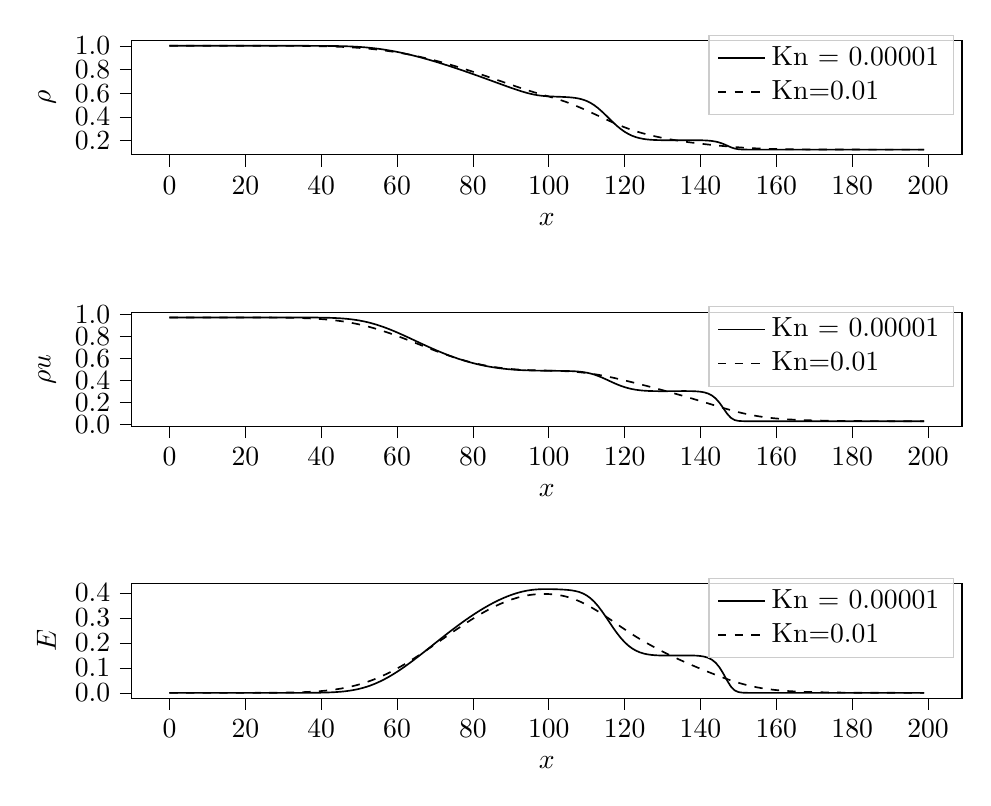
\begin{tikzpicture}

\begin{groupplot}[group style={group size=1 by 3, horizontal sep=2cm, vertical sep=2cm}]
\nextgroupplot[
legend cell align={left},
legend style={fill opacity=0.8, draw opacity=1, text opacity=1, at={(0.99,0.7)}, anchor=east, draw=white!80!black},
tick align=outside,
tick pos=left,
x grid style={white!69.0196078431373!black},
xlabel={\(x\)},
xmin=-9.95, xmax=208.95,
xtick style={color=black},
y grid style={white!69.0196078431373!black},
ylabel={\(\rho\)},
ymin=0.0812472272613489, ymax=1.04375013203517,
ytick style={color=black},
ytick={0,0.2,0.4,0.6,0.8,1,1.2},
yticklabels={0.0,0.2,0.4,0.6,0.8,1.0,1.2},
width=\textwidth,
height=.25\textwidth
]
\addplot [semithick, black]
table {%
0 0.999999999999998
1 0.999999999999989
2 0.999999999999973
3 0.999999999999938
4 0.999999999999854
5 0.999999999999657
6 0.999999999999225
7 0.999999999998307
8 0.999999999996346
9 0.999999999992153
10 0.999999999983302
11 0.999999999964812
12 0.999999999926618
13 0.999999999848593
14 0.999999999691032
15 0.999999999376523
16 0.999999998755951
17 0.999999997545765
18 0.999999995213722
19 0.999999990773699
20 0.999999982422727
21 0.999999966908873
22 0.999999938447061
23 0.999999886889466
24 0.999999794688685
25 0.999999631942622
26 0.999999348451367
27 0.999998861215854
28 0.99999803513588
29 0.999996653797842
30 0.999994376182765
31 0.999990673914891
32 0.999984742419316
33 0.999975378267931
34 0.999960814384862
35 0.999938505100111
36 0.999904854832319
37 0.999854888023955
38 0.99978186432473
39 0.999676852094109
40 0.9995282847065
41 0.999321536763255
42 0.999038569143143
43 0.998657700112069
44 0.998153561405535
45 0.997497290690344
46 0.996656993873317
47 0.99559848331206
48 0.994286264568487
49 0.992684710498992
50 0.990759333664029
51 0.988478051967666
52 0.98581234145918
53 0.982738184425117
54 0.979236747133095
55 0.975294754490673
56 0.970904562368228
57 0.966063957098391
58 0.960775732208377
59 0.955047103436866
60 0.948889025126006
61 0.942315466055067
62 0.935342693163985
63 0.927988599833952
64 0.920272103437352
65 0.912212626120219
66 0.903829663999579
67 0.895142443413195
68 0.886169658461554
69 0.876929281542178
70 0.867438437521144
71 0.857713332238945
72 0.847769226883468
73 0.837620451126894
74 0.827280449648232
75 0.816761858656435
76 0.806076611284112
77 0.795236073302906
78 0.784251213671778
79 0.773132818216759
80 0.761891759626233
81 0.750539343464475
82 0.739087758804205
83 0.727550674370907
84 0.715944038086624
85 0.704287161112698
86 0.692604198229712
87 0.680926174533778
88 0.669293749303168
89 0.657760935139416
90 0.646399961099968
91 0.635307285171405
92 0.62461023214634
93 0.614472547467368
94 0.605094999885858
95 0.596704255186181
96 0.58952161507939
97 0.583707951716951
98 0.579297599755217
99 0.576156316434373
100 0.574000969056694
101 0.572480179189811
102 0.571264203656635
103 0.570086382765471
104 0.568721460109119
105 0.566925165174661
106 0.564365792996614
107 0.560570509046267
108 0.554906055797055
109 0.546613499580239
110 0.534908971753206
111 0.51914228036301
112 0.498978621789052
113 0.474548680779275
114 0.446512149382244
115 0.416003356002158
116 0.384466862363659
117 0.35342828965285
118 0.324264603478363
119 0.298031575214768
120 0.275379774683857
121 0.25655829783077
122 0.241481617940157
123 0.229826469375018
124 0.221130574377751
125 0.214876145355647
126 0.210551637309679
127 0.207691967900792
128 0.205900479181207
129 0.204856774754392
130 0.204314508374631
131 0.204092813817174
132 0.204064484192581
133 0.204143252251004
134 0.204271660594381
135 0.204410149561804
136 0.204527209819603
137 0.2045897518297
138 0.204552165643129
139 0.204341777937618
140 0.203837534924661
141 0.202838126194388
142 0.201017076265398
143 0.197870634170907
144 0.192691647141719
145 0.184667360813301
146 0.173289806057922
147 0.159203831239715
148 0.144954929560638
149 0.134090936270534
150 0.128237751279186
151 0.125970039515887
152 0.125265822009891
153 0.125069122324036
154 0.125016332608434
155 0.125002354962472
156 0.12499867180924
157 0.124997703549099
158 0.124997449439354
159 0.124997382859364
160 0.12499736544419
161 0.124997360897239
162 0.124997359712403
163 0.124997359404317
164 0.124997359324391
165 0.124997359303707
166 0.124997359298369
167 0.124997359296995
168 0.124997359296643
169 0.124997359296553
170 0.12499735929653
171 0.124997359296525
172 0.124997359296523
173 0.124997359296523
174 0.124997359296523
175 0.124997359296523
176 0.124997359296523
177 0.124997359296523
178 0.124997359296523
179 0.124997359296523
180 0.124997359296523
181 0.124997359296523
182 0.124997359296523
183 0.124997359296523
184 0.124997359296523
185 0.124997359296523
186 0.124997359296523
187 0.124997359296523
188 0.124997359296523
189 0.124997359296523
190 0.124997359296523
191 0.124997359296523
192 0.124997359296523
193 0.124997359296523
194 0.124997359296523
195 0.124997359296523
196 0.124997359296523
197 0.124997359296523
198 0.124997359296523
199 0.124997359296523
};
\addlegendentry{Kn = 0.00001}
\addplot [semithick, black, dashed]
table {%
0 0.99999981316608
1 0.99999975421908
2 0.999999680296827
3 0.999999584015259
4 0.999999457570282
5 0.999999291316442
6 0.999999072816931
7 0.999998785865599
8 0.999998409307099
9 0.999997915549681
10 0.999997268671227
11 0.999996422006429
12 0.999995315081933
13 0.999993869739663
14 0.999991985257259
15 0.999989532239156
16 0.999986345012926
17 0.999982212224108
18 0.999976865280456
19 0.999969964255601
20 0.999961080825805
21 0.999949677785936
22 0.999935084677325
23 0.999916469067197
24 0.999892803054168
25 0.999862824644981
26 0.999824993762287
27 0.999777442809534
28 0.99971792194299
29 0.999643739485772
30 0.999551698263626
31 0.999438029040718
32 0.999298322672216
33 0.999127463048146
34 0.998919563350529
35 0.998667908546717
36 0.998364907354493
37 0.998002057094462
38 0.997569924850764
39 0.997058148157106
40 0.996455457989507
41 0.995749726175553
42 0.994928038439235
43 0.993976793230499
44 0.992881825300824
45 0.991628551759091
46 0.990202137164675
47 0.988587673176978
48 0.986770367464113
49 0.984735736041917
50 0.982469793006896
51 0.979959231754083
52 0.977191592215162
53 0.974155409371525
54 0.970840339230837
55 0.967237259535191
56 0.963338343623945
57 0.959137107042427
58 0.954628427617574
59 0.949808540774016
60 0.944675012808809
61 0.939226695650786
62 0.93346366726498
63 0.927387162272547
64 0.920999497473236
65 0.914303996700869
66 0.907304918741389
67 0.90000739086861
68 0.89241734896415
69 0.884541483383983
70 0.876387188096097
71 0.867962509719168
72 0.859276093668592
73 0.850337127400342
74 0.841155286214046
75 0.831740695052687
76 0.822103928898359
77 0.812256081874584
78 0.802208936708843
79 0.79197525683824
80 0.78156919951702
81 0.771006810236054
82 0.760306513523842
83 0.749489476246309
84 0.738579702514359
85 0.727603733467464
86 0.716589865685254
87 0.705566854549949
88 0.694562138954764
89 0.683599784307639
90 0.672698744484615
91 0.661872778856293
92 0.651134054393569
93 0.640501846359315
94 0.630014077905235
95 0.619732885281825
96 0.60973151025046
97 0.600058308646607
98 0.590696148720204
99 0.581551386384131
100 0.572476510359754
101 0.563293926378223
102 0.553800236231206
103 0.543781524364539
104 0.533063510452134
105 0.521566257579677
106 0.509313962288544
107 0.496400822236544
108 0.482943372019684
109 0.469048302365069
110 0.454804360618456
111 0.440289849071466
112 0.425583491928963
113 0.41077164651714
114 0.395950814468977
115 0.381227050612487
116 0.366713604395908
117 0.352527021957449
118 0.338781439243636
119 0.325581204566807
120 0.313012828321206
121 0.301137932019271
122 0.289988932118549
123 0.279568586970621
124 0.269853520854869
125 0.26080082760768
126 0.252356199651869
127 0.244461884500335
128 0.237063086804866
129 0.230112021380132
130 0.223569464145314
131 0.217404176438371
132 0.211590906449739
133 0.206107783930591
134 0.200933852741061
135 0.19604728678763
136 0.191424573503377
137 0.187040687492616
138 0.182870065685786
139 0.17888806575569
140 0.175072550584356
141 0.171405281352616
142 0.167872894069909
143 0.164467347431299
144 0.161185835445557
145 0.158030237217974
146 0.155006220934256
147 0.152122132077785
148 0.149387786605452
149 0.146813269947481
150 0.144407822244173
151 0.142178874538462
152 0.140131289623276
153 0.138266850742206
154 0.136584026151337
155 0.135078014784042
156 0.133741049493288
157 0.132562905381218
158 0.131531539089185
159 0.130633776435876
160 0.129855972071242
161 0.129184582884318
162 0.128606620847313
163 0.128109974484943
164 0.12768360662565
165 0.127317647528726
166 0.127003407220149
167 0.126733330622757
168 0.126500915923433
169 0.126300612357069
170 0.126127709374185
171 0.125978225574316
172 0.125848802984529
173 0.125736610164789
174 0.125639256072876
175 0.12555471547341
176 0.125481265823031
177 0.125417434945145
178 0.125361958389225
179 0.125313745129744
180 0.125271850176076
181 0.125235452709076
182 0.125203838498512
183 0.125176385551639
184 0.125152552162449
185 0.125131866744975
186 0.125113919022193
187 0.125098352293426
188 0.125084856614912
189 0.12507316280418
190 0.125063037227494
191 0.125054277361622
192 0.125046708146471
193 0.125040179165499
194 0.125034562672888
195 0.125029752262378
196 0.125025660897079
197 0.125022212914257
198 0.12501931099985
199 0.125016719545722
};
\addlegendentry{Kn=0.01}

\nextgroupplot[
legend cell align={left},
legend style={fill opacity=0.8, draw opacity=1, text opacity=1, at={(0.99,0.7)}, anchor=east, draw=white!80!black},
tick align=outside,
tick pos=left,
x grid style={white!69.0196078431373!black},
xlabel={\(x\)},
xmin=-9.95, xmax=208.95,
xtick style={color=black},
y grid style={white!69.0196078431373!black},
ylabel={\(\rho u\)},
ymin=-0.01673310421985, ymax=1.02222538591518,
ytick style={color=black},
ytick={-0.2,0,0.2,0.4,0.6,0.8,1,1.2},
yticklabels={−0.2,0.0,0.2,0.4,0.6,0.8,1.0,1.2},
width=\textwidth,
height=.25\textwidth
]
\addplot [semithick, black]
table {%
0 0.974999999999951
1 0.974999999999907
2 0.974999999999824
3 0.974999999999669
4 0.974999999999363
5 0.974999999998719
6 0.974999999997334
7 0.974999999994361
8 0.974999999988005
9 0.97499999997449
10 0.974999999946005
11 0.974999999886615
12 0.974999999764117
13 0.974999999514247
14 0.974999999010282
15 0.974999998005467
16 0.97499999602518
17 0.974999992168127
18 0.974999984744712
19 0.974999970628869
20 0.974999944113447
21 0.974999894919787
22 0.974999804790218
23 0.974999641748242
24 0.974999350589616
25 0.974998837398088
26 0.974997944775965
27 0.974996412947483
28 0.974993819843725
29 0.974989490653573
30 0.974982364144117
31 0.974970799467683
32 0.974952303544506
33 0.974923156099602
34 0.974877908067057
35 0.974808730775096
36 0.974704599839999
37 0.974550310877258
38 0.974325345523736
39 0.974002636439099
40 0.973547317759637
41 0.972915589234677
42 0.972053861336742
43 0.970898375644783
44 0.969375499011033
45 0.967402861802382
46 0.964891444638168
47 0.96174861692709
48 0.957882005938571
49 0.953203947485006
50 0.947636163508087
51 0.941114251262602
52 0.933591568377296
53 0.925042159926081
54 0.915462486128263
55 0.904871850402083
56 0.893311570998761
57 0.880843061635519
58 0.867545071311944
59 0.853510374501746
60 0.838842202878954
61 0.823650677707796
62 0.80804944992926
63 0.792152694582577
64 0.776072547066046
65 0.759917017309144
66 0.743788377532284
67 0.727781990715895
68 0.711985529261851
69 0.696478524726255
70 0.681332187714521
71 0.666609439914812
72 0.652365105973286
73 0.638646220052745
74 0.625492409437274
75 0.61293632476802
76 0.601004093017814
77 0.589715774934755
78 0.579085813345579
79 0.569123462430903
80 0.559833190932838
81 0.551215054311751
82 0.543265032207121
83 0.535975328229931
84 0.529334629143911
85 0.523328319872161
86 0.517938649476038
87 0.513144841329374
88 0.508923138416005
89 0.505246772903584
90 0.502085850252529
91 0.499407147401467
92 0.49717385201229
93 0.495345329402208
94 0.493877102148319
95 0.492721325732655
96 0.491827999856679
97 0.49114676049528
98 0.490628446577077
99 0.490225574411412
100 0.489892050726169
101 0.489583251617593
102 0.489255653552228
103 0.488862480126186
104 0.488342203004208
105 0.487599742148386
106 0.486483394633626
107 0.484763982379149
108 0.482126547018462
109 0.478186641198099
110 0.472539394541322
111 0.464838905549125
112 0.454891334433603
113 0.44273416486432
114 0.428673259277573
115 0.413260856638999
116 0.397217273102659
117 0.381317978552166
118 0.366277588773269
119 0.35265968586857
120 0.340828993937901
121 0.33094700235995
122 0.323000342106546
123 0.316846468366913
124 0.312262768652956
125 0.308989979885994
126 0.306765696589643
127 0.305347195468759
128 0.304524633083269
129 0.30412640615635
130 0.304018617899238
131 0.3041004451537
132 0.304296832802441
133 0.304549364882103
134 0.304805377771059
135 0.305004369236508
136 0.305059431344277
137 0.304829615323252
138 0.304076598389254
139 0.302395775284873
140 0.299109138529932
141 0.293110237613966
142 0.282676384199798
143 0.265350695775959
144 0.238216459608717
145 0.199238534917943
146 0.150286651533868
147 0.100222394985358
148 0.0619544979372982
149 0.0414884570530703
150 0.0337211704261632
151 0.0313715712541428
152 0.0307261916343882
153 0.030554080991312
154 0.030508566291402
155 0.030496565798877
156 0.030493407100338
157 0.0304925768893975
158 0.0304923590013502
159 0.0304923019056265
160 0.0304922869691739
161 0.0304922830687958
162 0.0304922820522722
163 0.0304922817879033
164 0.0304922817193052
165 0.0304922817015494
166 0.0304922816969657
167 0.0304922816957857
168 0.0304922816954828
169 0.0304922816954053
170 0.0304922816953855
171 0.0304922816953805
172 0.0304922816953792
173 0.0304922816953787
174 0.0304922816953786
175 0.0304922816953786
176 0.0304922816953786
177 0.0304922816953786
178 0.0304922816953786
179 0.0304922816953786
180 0.0304922816953786
181 0.0304922816953786
182 0.0304922816953786
183 0.0304922816953786
184 0.0304922816953786
185 0.0304922816953786
186 0.0304922816953786
187 0.0304922816953786
188 0.0304922816953786
189 0.0304922816953786
190 0.0304922816953786
191 0.0304922816953786
192 0.0304922816953786
193 0.0304922816953786
194 0.0304922816953786
195 0.0304922816953786
196 0.0304922816953786
197 0.0304922816953786
198 0.0304922816953786
199 0.0304922816953786
};
\addlegendentry{Kn = 0.00001}
\addplot [semithick, black, dashed]
table {%
0 0.97499875113314
1 0.974998415169894
2 0.974997973548605
3 0.974997395696738
4 0.974996641899692
5 0.974995660502251
6 0.974994384412448
7 0.974992726664499
8 0.974990574773972
9 0.974987783570467
10 0.974984166129488
11 0.974979482348512
12 0.974973424623592
13 0.974965599982967
14 0.974955507924868
15 0.974942513090756
16 0.974925811787139
17 0.974904391255565
18 0.974876980490849
19 0.974841991334292
20 0.974797448537848
21 0.974740907526093
22 0.97466935869869
23 0.974579117342472
24 0.974465698586819
25 0.974323677365753
26 0.97414653406921
27 0.973926487491382
28 0.973654317821857
29 0.973319183764751
30 0.972908439380017
31 0.972407457860469
32 0.971799471099136
33 0.97106543544448
34 0.970183935337622
35 0.969131137406915
36 0.967880807882504
37 0.966404405717162
38 0.964671262419475
39 0.962648857234242
40 0.960303192931419
41 0.957599273171241
42 0.954501677384405
43 0.950975223627868
44 0.94698570431875
45 0.942500674534815
46 0.937490268137065
47 0.931928013720771
48 0.925791620656961
49 0.919063705447127
50 0.911732430332963
51 0.903792029478882
52 0.895243202833517
53 0.886093363619209
54 0.876356731864906
55 0.866054273032626
56 0.855213487155596
57 0.84386805963105
58 0.832057389599166
59 0.819826015492807
60 0.807222959753423
61 0.79430101584967
62 0.781116000644616
63 0.767725993923634
64 0.754190584651331
65 0.740570140452826
66 0.726925113150936
67 0.713315389245721
68 0.699799690380289
69 0.686435025538408
70 0.673276194414801
71 0.660375340458305
72 0.647781552682338
73 0.635540517305218
74 0.623694223021033
75 0.612280726123241
76 0.601333982331972
77 0.590883749434623
78 0.580955557588194
79 0.571570732373029
80 0.562746441421245
81 0.554495723091702
82 0.546827451646118
83 0.539746204226656
84 0.533252023912799
85 0.527340116443966
86 0.522000563021953
87 0.517218158735683
88 0.51297247802311
89 0.509238219548044
90 0.505985803919417
91 0.503182108666139
92 0.500791138215919
93 0.498774346240497
94 0.497090293703681
95 0.495693485458681
96 0.494532791573075
97 0.493550752015684
98 0.492685458641156
99 0.491875397221745
100 0.491063189151311
101 0.490192977065561
102 0.48920240833866
103 0.48801792701956
104 0.486559505870383
105 0.484751844540064
106 0.482534111769432
107 0.479863840425919
108 0.476715068312198
109 0.473073625302302
110 0.468932454586416
111 0.464288498291381
112 0.459141567287615
113 0.453495132690942
114 0.447358709553042
115 0.440751104851276
116 0.433703342296002
117 0.426259875726154
118 0.418477015585467
119 0.410418308357704
120 0.402147641706951
121 0.3937216832974
122 0.385183559113504
123 0.376559330481685
124 0.367857995626125
125 0.359074747562422
126 0.350196402787923
127 0.341207494217294
128 0.332095550716605
129 0.322854479424428
130 0.313485565917444
131 0.303996237370641
132 0.294397248222027
133 0.284699248153887
134 0.274909738528037
135 0.265031235221812
136 0.255061102884695
137 0.244993108117227
138 0.234820360234526
139 0.224539047924846
140 0.214152277132536
141 0.203673364300637
142 0.193128099257836
143 0.182555705807116
144 0.17200843930401
145 0.161549929075766
146 0.151252482363223
147 0.141193620534845
148 0.131452136981804
149 0.122103971697478
150 0.113218204188991
151 0.104853473161649
152 0.0970551232812204
153 0.0898533357764977
154 0.0832624078544069
155 0.0772812112449471
156 0.0718947081102429
157 0.0670762697556515
158 0.0627904630120332
159 0.0589959567229227
160 0.0556482505762533
161 0.0527020179630825
162 0.0501129551777841
163 0.047839117332109
164 0.0458417835990838
165 0.0440859284106123
166 0.0425403860195424
167 0.0411777914618226
168 0.0399743690741606
169 0.0389096258225613
170 0.0379659937860883
171 0.0371284552980005
172 0.0363841754338102
173 0.0357221592919263
174 0.0351329453915581
175 0.0346083412653218
176 0.0341412029025281
177 0.0337252561734085
178 0.0333549558222661
179 0.0330253760883323
180 0.0327321264328573
181 0.0324712860639916
182 0.0322393517382954
183 0.0320331944366773
184 0.0318500217358559
185 0.0316873438412782
186 0.031542942191471
187 0.0314148402277158
188 0.0313012763423488
189 0.0312006792098562
190 0.0311116457266017
191 0.0310329217043195
192 0.0309633853412159
193 0.030902033380718
194 0.0308479697903068
195 0.030800396753786
196 0.0307586077265718
197 0.0307219821085531
198 0.0306899803444434
199 0.0306621360327894
};
\addlegendentry{Kn=0.01}

\nextgroupplot[
legend cell align={left},
legend style={fill opacity=0.8, draw opacity=1, text opacity=1, at={(0.99,0.7)}, anchor=east, draw=white!80!black},
tick align=outside,
tick pos=left,
x grid style={white!69.0196078431373!black},
xlabel={\(x\)},
xmin=-9.95, xmax=208.95,
xtick style={color=black},
y grid style={white!69.0196078431373!black},
ylabel={\(E\)},
ymin=-0.0207805766857379, ymax=0.436392110400496,
ytick style={color=black},
ytick={-0.1,0,0.1,0.2,0.3,0.4,0.5},
yticklabels={−0.1,0.0,0.1,0.2,0.3,0.4,0.5},
width=\textwidth,
height=.25\textwidth
]
\addplot [semithick, black]
table {%
0 6.30909942701128e-15
1 2.52743810784534e-14
2 6.71665952599217e-14
3 1.47797315819247e-13
4 3.07924884094236e-13
5 6.61724731226376e-13
6 1.42564590793223e-12
7 3.07415836396623e-12
8 6.61513600596091e-12
9 1.41586576150479e-11
10 3.00685205419515e-11
11 6.32804201327425e-11
12 1.3184036970615e-10
13 2.71816269673475e-10
14 5.54376851469977e-10
15 1.11825149908461e-09
16 2.23051509342037e-09
17 4.39884368497434e-09
18 8.5758772306255e-09
19 1.65259662279758e-08
20 3.14735318416989e-08
21 5.92319223420021e-08
22 1.10138321629211e-07
23 2.02317178115227e-07
24 3.67093738893431e-07
25 6.57821443877529e-07
26 1.16402288185517e-06
27 2.03362897054613e-06
28 3.50728901639945e-06
29 5.97025142461952e-06
30 1.00291759427997e-05
31 1.66233527041188e-05
32 2.71819700399184e-05
33 4.38409224509142e-05
34 6.97336019227715e-05
35 0.000109369363494647
36 0.000169109905168177
37 0.000257746596586162
38 0.000387169951738958
39 0.000573105629364502
40 0.00083587020550754
41 0.00120107655052603
42 0.00170019665307498
43 0.00237087432492865
44 0.0032568772432988
45 0.00440759238754277
46 0.00587700375526764
47 0.00772214479508426
48 0.0100010837905844
49 0.0127705676361399
50 0.0160835050774659
51 0.0199865027249069
52 0.0245176686528201
53 0.0297048684855691
54 0.0355645636560769
55 0.0421012920749302
56 0.0493077806620858
57 0.0571656185418088
58 0.065646376882973
59 0.074713039379489
60 0.0843216049455656
61 0.0944227371486421
62 0.10496335769442
63 0.115888108463717
64 0.127140633730189
65 0.138664658219507
66 0.150404855967261
67 0.162307519006456
68 0.17432104407487
69 0.186396260539237
70 0.198486624527203
71 0.210548303768142
72 0.222540175680823
73 0.234423758453756
74 0.246163091716497
75 0.257724580217212
76 0.269076810899138
77 0.280190351007068
78 0.291037532389737
79 0.301592224987379
80 0.311829600578427
81 0.32172588617664
82 0.33125810501847
83 0.340403801924414
84 0.349140749159004
85 0.357446629223257
86 0.365298693275803
87 0.372673400036284
88 0.379546053737188
89 0.385890487528712
90 0.391678891683233
91 0.396881980082096
92 0.40146984092481
93 0.405414027071735
94 0.408691633111172
95 0.411292026446267
96 0.413226031432564
97 0.414535188150287
98 0.415295778738166
99 0.415611533714758
100 0.415593775426746
101 0.415336272676748
102 0.414895448502171
103 0.414279737593578
104 0.413441915625134
105 0.412265559121292
106 0.410543071971494
107 0.407952686344571
108 0.404050222699679
109 0.398294145414728
110 0.390116261831736
111 0.379034708912469
112 0.364785477913794
113 0.347433285813965
114 0.327421674382695
115 0.305538967700042
116 0.282804901002568
117 0.260309644556986
118 0.239050562602313
119 0.21980754302411
120 0.203079346386846
121 0.189081108100233
122 0.177786617803809
123 0.168993000834794
124 0.162388542023055
125 0.157611733202854
126 0.15429658772856
127 0.152103712729153
128 0.150738704834072
129 0.149960168581477
130 0.149579859369824
131 0.149457422785557
132 0.149491944246978
133 0.149612013943466
134 0.14976530020989
135 0.149907791760532
136 0.14999195731766
137 0.14995203609554
138 0.149683391775078
139 0.149011229469267
140 0.147642220299706
141 0.145092234771363
142 0.140589880897931
143 0.132983874719494
144 0.12076396568901
145 0.102471387896822
146 0.0779153049527428
147 0.0500927747148544
148 0.0255869635272696
149 0.0101029770633572
150 0.00323067179465287
151 0.000916685484344893
152 0.000247535673412993
153 6.57015398035193e-05
154 1.73347678877712e-05
155 4.56166544163445e-06
156 1.19832317827514e-06
157 3.14296212372224e-07
158 8.22998347460696e-08
159 2.15132337412575e-08
160 5.61307173932267e-09
161 1.46156536596175e-09
162 3.79741252383841e-10
163 9.84313849249286e-11
164 2.54493090390674e-11
165 6.56196973336829e-12
166 1.68704997701825e-12
167 4.32438917614844e-13
168 1.10497771029924e-13
169 2.81771756164485e-14
170 7.1446327166275e-15
171 1.78835623869184e-15
172 4.08881037663235e-16
173 5.2382325353727e-17
174 2.23070013203397e-18
175 -1.70270270785549e-18
176 1.91820140579613e-19
177 -2.40410876608015e-18
178 -2.60371401563257e-18
179 1.34734438717905e-19
180 1.35175634880655e-19
181 1.35610010757515e-19
182 1.35610010757515e-19
183 1.35610010757515e-19
184 1.35610010757515e-19
185 1.35610010757515e-19
186 1.35610010757515e-19
187 1.35610010757515e-19
188 1.35610010757515e-19
189 1.35610010757515e-19
190 1.35610010757515e-19
191 1.35610010757515e-19
192 1.35610010757515e-19
193 1.35610010757515e-19
194 1.35610010757515e-19
195 1.35610010757515e-19
196 1.35610010757515e-19
197 1.35610010757515e-19
198 1.35610010757515e-19
199 1.35610010757515e-19
};
\addlegendentry{Kn = 0.00001}
\addplot [semithick, black, dashed]
table {%
0 4.54455299100046e-07
1 5.99854726306051e-07
2 7.8833937943175e-07
3 1.03258649420672e-06
4 1.34970552357957e-06
5 1.76218162719785e-06
6 2.29933730512723e-06
7 2.9993028510072e-06
8 3.91157902756794e-06
9 5.10032659340901e-06
10 6.64856011169223e-06
11 8.66346749193427e-06
12 1.1283125362535e-05
13 1.46849349680372e-05
14 1.90961639813164e-05
15 2.48070458569648e-05
16 3.21869585645296e-05
17 4.17042761626466e-05
18 5.39505557152346e-05
19 6.96697830363863e-05
20 8.97934463024172e-05
21 0.000115482227362561
22 0.00014817508525939
23 0.00018964644172765
24 0.000242072049645008
25 0.000308103917080716
26 0.000390954356975003
27 0.000494488822951434
28 0.000623326667101406
29 0.000782948314726992
30 0.000979806602457875
31 0.00122143919118749
32 0.00151657807971254
33 0.00187525136096786
34 0.00230887154792676
35 0.00283030413169527
36 0.0034539096093941
37 0.00419555212427541
38 0.00507256817627539
39 0.00610368964860908
40 0.00730891668390221
41 0.00870933771887943
42 0.0103268961885164
43 0.0121841059281862
44 0.0143037199803669
45 0.0167083601629121
46 0.0194201171751697
47 0.0224601330085379
48 0.0258481788193049
49 0.0296022420910958
50 0.0337381368008472
51 0.0382691494128088
52 0.0432057319324069
53 0.0485552510840276
54 0.0543218001007408
55 0.0605060768152644
56 0.0671053289042067
57 0.0741133644279057
58 0.0815206233628243
59 0.0893143037460852
60 0.0974785344151436
61 0.105994585179522
62 0.11484110464153
63 0.123994375817061
64 0.133428580216276
65 0.143116062129349
66 0.153027586486912
67 0.163132585720724
68 0.173399393329266
69 0.183795464026721
70 0.194287581980226
71 0.204842059214592
72 0.215424925325016
73 0.226002106937574
74 0.236539591075874
75 0.247003561570937
76 0.257360493548
77 0.26757719026068
78 0.277620751863024
79 0.287458479192157
80 0.297057737197227
81 0.306385828460686
82 0.315409948964838
83 0.324097304272163
84 0.332415443906881
85 0.340332821288337
86 0.347819514440552
87 0.35484796821436
88 0.361393562340091
89 0.367434779748903
90 0.372952744621367
91 0.377929946520065
92 0.38234818701995
93 0.386186388267707
94 0.389419925219161
95 0.392023892303592
96 0.393981528311944
97 0.395294661906065
98 0.395987922268566
99 0.396099555689399
100 0.395658926713393
101 0.394662325272313
102 0.393063105985357
103 0.390783106753753
104 0.387738698310261
105 0.383869352121223
106 0.379155360021045
107 0.373617300375614
108 0.367302890237123
109 0.360271900192528
110 0.352586216657906
111 0.344306227834089
112 0.335491444318213
113 0.326203075092749
114 0.316507210045428
115 0.306477788664165
116 0.296198458188714
117 0.285762282447909
118 0.275268551155491
119 0.264816737359117
120 0.25449865135719
121 0.244390587135066
122 0.234547408729126
123 0.225000011467603
124 0.215756633727468
125 0.206807461416989
126 0.198131207855713
127 0.189702055952046
128 0.181495515904338
129 0.173492239971993
130 0.165679454368033
131 0.158050244841829
132 0.150601350337783
133 0.143330323194121
134 0.136232903033059
135 0.129301264291135
136 0.122523501442489
137 0.115884390612929
138 0.1093671852864
139 0.102956019759651
140 0.0966384287463818
141 0.0904075357375704
142 0.0842635839007025
143 0.0782146386186505
144 0.0722764400425698
145 0.0664714991620224
146 0.0608275999986637
147 0.0553758968537104
148 0.0501487924591837
149 0.045177766924436
150 0.0404913114022774
151 0.0361131090887707
152 0.0320605952695308
153 0.0283440079834433
154 0.0249660027875256
155 0.0219218475058126
156 0.0192001440166512
157 0.0167839597388279
158 0.0146522080278887
159 0.0127811044806488
160 0.0111455453501796
161 0.00972029590602644
162 0.00848092707308504
163 0.00740448534503526
164 0.00646991565985121
165 0.00565827705059631
166 0.00495279816714197
167 0.00433881810166761
168 0.00380365148512002
169 0.00333640878221297
170 0.00292779505335359
171 0.00256990402128406
172 0.00225601920638259
173 0.00198042996503681
174 0.00173826719329184
175 0.00152536101752409
176 0.00133812085700574
177 0.00117343675845373
178 0.00102859985494394
179 0.00090123917588212
180 0.000789271794310028
181 0.000690863378432377
182 0.000604396530399906
183 0.00052844475296431
184 0.000461750394540807
185 0.000403205412331374
186 0.000351834210560911
187 0.000306778129286099
188 0.000267281372367963
189 0.000232678280462438
190 0.000202381895071296
191 0.000175873744959299
192 0.000152694737618318
193 0.00013243697449953
194 0.000114736251193023
195 9.92650033574736e-05
196 8.57256827296962e-05
197 7.38455370907372e-05
198 6.33771043745151e-05
199 5.41183398169117e-05
};
\addlegendentry{Kn=0.01}
\end{groupplot}

\end{tikzpicture}

	\caption{Macroscopic quantities \(rho\), \(\rho u\) and \(E\) in the SOD schock tube at the last time stamp. The quantites are displayed for the hydrodynamic regime in - - lines and for the rarefied regime in - lines.}
\end{figure}
- intrinsic code variables for hydro an rare add pls
\section{Deep learning}
In this section deep learning with the focus on fully connected autoencoders and convolutional autoencoders will be introduced. Starting of with addressing important terminology whilst presenting the concept of autoencoders and continuing with the introduction of the fully connected and convolutional forwardpass , this section closes with ADAM \cite{the} an update to the backpropagation algorithm as well as important training methods.\\ 
The term deep learning situated around the much broader field of artificial intelligence stems from the use of deep feed forward networks also called multi layer perceptrons (MLP) or feed forward neural networks. Deep recurrent neural networks (RNN) are also used in this field but won't be covered in this thesis. In contrast to RNNs, information flows forward through these networks, which explains the name feed foward. In the following I will use the abbreviation MLP when talking about the aforementioned algorithm. Network refers to the typical composition of many different functions.\\The task of any MLP is to approximate a function \(f^\star(\mathbf{x};\mathbf{\Theta}) \approx f(\mathbf{x})\) through learning the values of the parameters \(\mathbf{\Theta}\). As mentioned before  \(f^\star\) is a composition of functions eg. \cref{Eq. Composition}.
\begin{equation}
	 f^\star(\mathbf{x};\mathbf{\Theta})= f^3(f^2(f^1(\mathbf{x};\mathbf{\Theta}^1),\mathbf{\Theta}^2),\mathbf{\Theta}^3)
	 \label{Eq. Composition}
\end{equation}
 In \cref{Eq. Composition} each function \(f^i\) is called layer. In this example \(f^1\) is called the input layer, \(f^3\) the output layer and \(f^2\) a hidden layer. Hence a layer is a vector-to-vector function. In this context a unit describes the corresponding vector-to-scalar functions of one layer. The width of a layer is referred to as the dimension of the vector valued input. The depth of the network describes the number of composed functions. In autoencoders the dimensions of input and output layer are identical.\\Autoencoders are a special kind of neural network, that have a central hidden layer, that outputs a code \(c\) which should contain useful features of the input \(x\) while usually being of a lower dimension. Hereafter the code will be addressed as intrinsic variables highlighting the property of containing useful features of the input \(x\). Autoencoders can be split in two parts, the encoder \(h(x) = c\) which compresses the input and outputs the intrinsic variables \(c\) and the decoder \(g(h) = \hat{x}\) which reconstructs the input from the intrinsic variables to output \(\hat{x}\). The goal of autoencoders conflicts with the training objective. The former is to produce a code that describes the intrinsic features of the input, while the latter is to minimize the difference between \(x\) and \(\hat{x}\). Therefore autoencoders need to be restrained from learning the identity function perfectly which in turn should drive the model to choose which instance to copy.\\
Obviously deep learning emphasizes the focus on the depth of a model. This is because linear models with just one layer can only approximate linear functions. Adding a non-linear activation function to the output of the proposed model wouldn't be sufficient in modeling any nonlinear behavior of the function. However the universal approximation theorem \cite{Hornik1989} states that MLPs with at least one hidden layer and any non-linear activation function can approximate any function given that enough hidden layers can be provided. In conclusion, MLPs are universal approximators \cite{Goodfellow}.\\
There are several types of layers, that can be used in MLPs. For this thesis it is sufficient to treat so called \textit{fully connected layers} and \textit{convolutional layers}.
Fully connected layers are called \texttt{Linear}\cite{bibid} in \texttt{PyTorch}\cite{bibid} because they compute a linear transformation of the input \cref{Eq. Linear Transformation}, where \(x\) is the input vector, \(A\) is the weight matrix and \(b\) is a bias vector. This is the forward pass of a linear layer. The learnable parameters \(\Theta\) are in this case the values in \(A\) and \(b\). For a linear layer which takes a vector of size \(i\) as input and outputs a vector of size \(o\) there are \(l = i \times o + o\) learnable parameters. 
\begin{equation}
	y = xA^T + b \label{Eq. Linear Transformation}
\end{equation}
Continuing with the forward pass in convolutional layers, which are called \texttt{Conv2D}\cite{bibid} in \texttt{Pytorch}. Convolutional layers are usually applied when the input data has a known grid-like topology \cite{Goodfellow}.While for fully connected layers, the input size is fixed, convolutional layers can be applied to inputs of various sizes. Furthermore, they are sparse by construction and share parameters making them equivariant \cite{Goodfellow}.  Even tough the name implies the use of the convolutional operation in \cref{Eq. Convolution}, \texttt{PyTorch} and many other neural network libraries instead use the cross correlation, which is an operation closely related to a convolution\cite{Goodfellow}\cite{Pytorch website}. The convolution in \ref{Eq. Convolution} operates on two functions \(x\) and \(w\), where the latter is a weighting function of the former which makes \(s\) the weighted average of the input \(x\). In \cref{Eq. Discrete Convolution} \(x\) is represented by \(I(m,n)\), and \(w\) by \(K(m,n)\) respectively. Note that while \cref{Eq. Convolution} is scalar valued and \cref{Eq. Discrete Convolution} is two dimensional, only for illustrative reasons. 
\begin{align}
	s(t) &= (x * w)(t) = \int x(a)w(t-a)\,da \label{Eq. Convolution}\\
	S(i,j) &= (I * K)(i,j) = \sum_{m}\sum_{n}I(m,n)K(i-m,j-n)
	\label{Eq. Discrete Convolution}
\end{align}
One drawback in implementing the discrete convolution \cref{Eq. Discrete Convolution} is that there can be invalid values for \(m\) and \(n\). This can be solved by exploiting the commutative property of the convolution, which results for the discrete convolution in a flipped kernel relative to the input, \cref{Eq. Discrete Convolution Flip}. Without the need of flipping the kernel which is not always possible, i.e. exploiting the commutative property, cross correlation is adopted \cref{Eq. Discrete Cross Correlation}.
\begin{align}
	S(i,j) &= (K * I)(i,j) = \sum_{m}\sum_{n}I(i-m,j-n)K(m,n) 
	\label{Eq. Discrete Convolution Flip}\\
	S(i,j) &= (I * K)(i,j) = \sum_{m}\sum_{n}I(i+m,j+n)K(m,n) 
	\label{Eq. Discrete Cross Correlation}
\end{align}
The given equations illustrate the movement of the kernel over a two dimensional input, but leaving out two basic accompanying designs. First is the so called stride of the kernel, which results in a increased down sampling with increased stride size. Considering strides of the kernel along one dimension of the input results in a shrinkage of that dimension by 
\begin{equation}\label{Eq:Downsampling}
	o = \frac{i -k}{s} + 1.
\end{equation} 
Here \(o\), \(i\), \(s\) and \(k\) are the output, input, stride and kernel size of one dimension respectively \cite{dumoulin2018guide}. Second are the so called channels, which allow convolutional layers to extract a different feature for every channel from the same input. For a two dimensional input like images this could be different features for the same location on the image, like edges and color in the RGB color space \cite{Goodfellow}. Adding strides and kernel to \cref{Eq. Discrete Cross Correlation} yields
\begin{equation}
	\mathsf{S}_{i,j,k} = c(\mathsf{K},\mathsf{I},s)_{i,j,k}\sum_{l,m,n}\left[\mathsf{I}_{l,(j-1)\times s+m,(k -1)\times s+n}\mathsf{K}_{i,l,m,n}\right]. \label{Eq. Cross correlation stride channel}
\end{equation}
The kernel \(\mathsf{K}\) is a four dimensional tensor with \(i\) indexing into the output channels of \(S\), \(l\) indexing into the input channels of \(I\), \(m\) and \(n\) indexing into the rows and colums. The input \(\mathsf{I}\) and output \(S\) are three dimensional tensors with \(j\) and \(k\) indexing into the rows and columns. Note that in \texttt{PyTorch} \cref{Eq. Cross correlation stride channel} is a so called valid cross correlation (valid convolution) \cite{bibid} meaning the kernel will only move over input units for which  all \(m\) and \(n\) are inside the rows and columns of the input. Zero padding the input can prevent the kernel from omitting corners in that case.
\\
For autoencoders the necessity to perform a transposition of the applied layers arises, which is straight forward for fully connected layers. Convolutional layers with strides greater than unity on the other hand  the transposition needs the kernel to be padded with zeros to realize an upsampling of the input data \cite{dumoulin2018guide}. Note that the padding of the kernel with zeros is only used to illustrate how the upsampling works. In \cref{Eq: Transposed convolution} taken from \cite{Goodfellow} multiplications with zero are omitted. The size of one dimension during upsampling can be calculated with the transposition of \cref{Eq:Downsampling}.
\begin{equation}\label{Eq: Transposed convolution}
	t(\mathsf{K},\mathsf{H},s)_{i,j,k} = \sum_{\substack{l,m\\s.t\\(l-1)\times s+m=j}}
												  \sum_{\substack{n,p\\s.t\\(n-1)\times s+p=k}}
												  \sum_q \mathsf{K}_{q,i,m,p}\mathsf{H}_{q,l,n} 
\end{equation}
\noindent
Forward-propagation is then referred to as the compositional evaluation of each layer. For the example in \cref{Eq. Composition} the outputs of each layer would then be:  \(f^1(\mathbf{x},\mathbf{\Theta}^1) = \mathbf{p}\), \(f^2(\mathbf{p},\mathbf{\Theta}^2) = \mathbf{q}\) and \(f^3(\mathbf{q},\mathbf{\Theta}^3) = \mathbf{\hat{y}}\).\\
Subsequently the cost function \(J(\Theta)\), which will be discussed later on, can be computed. Afterwards back-propagation returns the gradients w.r.t. the layer parameters \(\Theta\) to finally compute updated parameters \(\mathbf{\Theta}\).  The name back-propagation refers to the use of the chain rule of calculus to obtain the gradients of each layer. Assuming again the example in \cref{Eq. Composition} back-propagation would be equations \cref{Eq. Backpropagation1} to \cref{Eq. Backpropagation3}:
\begin{align}
	\frac{\partial J}{\partial \mathbf{\Theta}^3} &= \frac{\partial J}{\partial\hat{y}_i}\frac{\partial\hat{y}}{\partial \Theta^3}
\label{Eq. Backpropagation3}\\
	\frac{\partial J}{\partial \Theta^2} &= \frac{\partial J}{\partial\hat{y}}\frac{\partial\hat{y}}{\partial q}\frac{\partial q}{\partial \Theta^2}
\label{Eq. Backpropagation2}\\
	\frac{\partial J}{\partial \mathbf{\Theta}^1} &= \frac{\partial J}{\partial\hat{y}}\frac{\partial\hat{y}}{\partial q}\frac{\partial q}{\partial p}\frac{\partial p}{\partial \Theta^1}
\label{Eq. Backpropagation1}
\end{align}
While the term back-propagation is solely used for the method to compute the gradients for each layer in a backward fashion, meaning form the last layer to the first, the update of the parameters is done in an optimization step.
-L2-error as perfomance metrics
\section{Reduced Order Algorithms}
In this section model order reduction (ROM) will be introduced and two algorithms for obtaining a reduced basis (RB) are discussed. The singular value decomposition (SVD) and autoencoders. In addition a reduced order model (ROM) based on the method of characteristics\cite{CFD1} is evaluated.\\
Model order reduction is a technique used for reducing a computational cost, which is computational resources as memory and computation power, and the time needed to compute a solution. Model order reduction exploits the idea that every high dimensional dynamical-state space\(f(\mathbf{x},\mathbf{\mu}) \in \mathcal{D}\)  can be described by a state-space or manifold of lower rank \(\tilde{f}(\mathbf{\mu}) \in \mathcal{E}\)
\begin{equation}
	f \approx \tilde{f} \qquad\textrm{with}\qquad \mathcal{D} \ll \mathcal{E}.
\end{equation}
Reduced order modeling is partitioned into two successive phases called the \textit{offline} - and the \textit{online phase}. During the offline phase data or \textit{snapshots} of a dynamical-system is generated through experiments or simulations of the full order model (FOM). The so called \textit{snapshots} \(U = {u(t1),...,u(t_n)}\) are created once, each representing one moment in time of the dynamical system. Next a mapping \(g\) is constructed such that \(\tilde{u} = g(\tilde{u})\), for which \(u(t_i) \approx u(t_i)\). During the online phase the reduced order model is evaluated and the error is estimated by eg. \(||u(t) - \tilde{u}(t)\). Therefore the online phase may be described as stage of independence from the full order model. 
To continue the definition of the \textit{intrinsic solution manifold dimensionality} by \textit{Carlberg et al.} \cite{Carlberg} is needed: Assuming the initial value problem
\begin{equation}
	\mathbf{r}^n(\mathbf{x}^n;\mathbf{\mu}) = 0, \qquad n=1,...,N_t
\end{equation} 
has a unique solution for each parameter instance \(\mathbf{\mu} \in \mathcal{D}\), the intrinsic dimensionality of the solution manifold \(\{\mathbf{x}(t,\mathbf{\mu})|t \in [0,T],\mathbf
\mu \in \mathcal{D}\}\) is (at most) \(p^{\star} = n_{\mu} + 1\), as a mapping \((t,\mathbf{\mu})\mapsto \mathbf{x}\) is unique in this case. This provides a practical lower bound on the dimension of a nonlinear trial manifold for exactly representing the dynamical-system state. In summary the intrinsic solution manifold dimensionality, in the following referred to as the number of intrinsic variables, are in number as much as there are parameters that can describe the whole dynamical-system state plus one, the time \(t\). As for the full order BGK equation \cref{Sec: BGK} the intrinsic variables could be six for the macroscopic velocity \(U(\mathbf{x},t)\), six for the microscopic velocities \(\xi\)of the collision operator \(Q(f,f)\), three for \(T\),\(\rho\) and \(\nu\) plus one equaling to a total of ten intrinsic variables for the 3D case. In the following subsection the available data for this thesis is introduced along with a proposal for the number of intrinsinc variables.\\
The BGK equation is valid for gases in the hydrodynamic regime as well as for rarefied gases. As described in \cref{Sec: BGK} depending on the equilibrium of the BGK equation, the solution transitions between a pure Boltzmann - and a Maxwellian distribution. The former is known to be well approximated by linear methods as the SVD, while the latter poses problems due to the non-linear behavior. 
\subsection{Data Sampling}\label{Sec: Data Sampling}
DIE ORIGINAL DTATENSTRUJTUR BESCHREIBEN
For the autencoder using fully connected layers, the input vectors $y_o \in \mathbb{R}$ of size $n_{\text{input}} = n_{\xi} = 40$ are arranged in the sampling matrix $S_{AE} \in \mathbb{R}^{n_{\mathrm{S}\times n_\xi}}$ as seen in \cref{AE_matrix} resulting in $n_S = 5000$ available samples. Note that the POD uses the same matrix transposed $S_{AE}^T$ as input. In the following hydrodynamic regime will reffer for the input data for knudsen number 10e-4 and rarefied regime will refer to the input data for knudsen numbers 10e2.
- insert unshuffled set pls
\begin{multicols}{2}
	\begin{equation}
	S_{AE} = \begin{bmatrix}
	f(\xi_1,t_1,x_1)&\cdots &f(\xi_n,t_1,x_1) \\
	f(\xi_1,t_1,x_2)&\cdots &f(\xi_n,t_1,x_2) \\
	\vdots& \vdots & \vdots\\
	f(\xi_1,t_1,x_n)&\cdots &f(\xi_n,t_1,x_n)\\
	f(\xi_1,t_2,x_1)&\cdots &f(\xi_n,t_2,x_1)\\
	\vdots & \vdots & \vdots\\
	f(\xi_1,t_n,x_n)&\cdots &f(\xi_n,t_n,x_n)
	\end{bmatrix}
	\label{AE_matrix}
	\end{equation}\break
	\begin{equation}
	S_{Conv}= \begin{bmatrix}
	n_{Filters}&f(\xi_1,\textbf{t},\textbf{x})\\
	n_{Filters}&f(\xi_2,\textbf{t},\textbf{x})\\
	\vdots\\
	n_{Filters}&f(\xi_n,\textbf{t},\textbf{x})
	\end{bmatrix}
	\label{Conv_matrix}
	\end{equation}
\end{multicols}\noindent
Convolutional autoencoders use a different sampling matrix $S_{Conv}$ due to their two dimensional capability resulting in $n_S = 40$ available samples \cref{Conv_matrix}.$N_{Filters}$ varies over the succeeding layers, growing with the shrinkage of $(\textbf{t},\textbf{x})$.
\subsection{POD}
The singular value decomposition of the input $X$ [REF to Section 1] gives the optimal low-rank approximation $\tilde{X}$ of $X$ \cref{Eg:eckard-young}[Eckard-Young]. 
\begin{equation}
\underset{\tilde{X}, s.t. rank(\tilde{X})=r}{\operatorname{argmin}} || X -\tilde{X} ||_F=\tilde{U}\tilde{\Sigma}\tilde{V}^*
\label{Eg:eckard-young}
\end{equation}
\subsection{Autoencoders}

Autoencoders have many hyperparameters determining their capability for compression and subsequent reconstruction. These parameters include : \textit{depth}, \textit{width of layers}, \textit{activation functions}, \textit{batch-size}, \textit{learning rate}, \textit{number of filters}, \textit{stride width}, \textit{kernel size}. Their finding is discussed in this section, for both hydrodynamic and rarefied input data.\\
\subsubsection{Hyperparameters for the Fully Connected Autoencoder}\label{Fully Connected}
To start with a working model an educated guess is made about the initial design of the architecture. \Cref{Tab: First Guess} shows chosen hyperparameters  which are used initially.
\begin{table}[!htbp]\centering
	\begin{tabular}{ |c|c|c|c|c| }
		\hline
		Mini batch size & Intrinsic dimensions& Epochs & Learing rate & activation code/rest\\ [.5ex]
		\hline
		16 & 3 & 2000& 1e-4 & Tanh/leakyreLU\\ \hline
	\end{tabular}
	\caption{Initial hyperparameter selection}
	\label{Tab:First Guess}
\end{table}
Originally the number of layers is determined, as they set a consequential part of the representational capacity of the model and therefore can initiate over- and underfitting at an early stage of the parameter search. \Cref{Fig:Layer_Size} and \cref{Fig:Layer Size Rare} in \cref{AppendixA} show the training and validation error for five designs shown in \cref{Tab:Layer Size}.\\
\begin{table}[!htbp]\centering
	\begin{tabular}{ |c|c| }
		\hline
		Number of layers & Reduction per layer \\ [.5ex]
		\hline
		10 & 40 \(\rightarrow\) 40 \(\rightarrow\) 20  \(\rightarrow\) 10 \(\rightarrow\) 5 \(\rightarrow\) 3\\ \hline
		8 & 40 \(\rightarrow\) 40 \(\rightarrow\) 20  \(\rightarrow\) 10 \(\rightarrow\) 3\\ \hline
		6 & 40 \(\rightarrow\) 40 \(\rightarrow\) 20  \(\rightarrow\) 3\\ \hline
		4 & 40 \(\rightarrow\) 40 \(\rightarrow\) 3\\ \hline
		2 & 40 \(\rightarrow\) 3\\ \hline
	\end{tabular}
	\caption{Initial hyperparameter selection}
	\label{Tab:Layer Size}
\end{table}
For the hydrodynamic regime a number of layers greater than four results in a slight overfitting at an early stage of training (at around 100 epochs). Below four layers an underfitting can be observed. Hence yielding the conclusion, that four layers result in the best perfoming net at this early stage. Overfitting occurs only after the 1000th epoch and is less than with the other three nets that show overfitting. Note, that contrary to expected results, the train error is lower than the test error. The random shuffling during preprocessing might be taken into account here. Nonetheless solely overfitting is defined by differences between train and test loss. In Addition four layers and lower show a stable training in relation to the rest.\\
The analysis of the number of layers for the rarefied regime is not showing overfitting as obvious as before. The network with two layers underfits in contrast to the other nets whereas nets with more than two layers reach a similar train - and test loss. Networks with more than 4 layers, again show an unstable training compared to the net with four layers. Train and test loss show a diverging behaviour after around the 100th epoch.\\
In conclusion the net with four layers performs best for both the hydrodynamic and the rarefied regime.\\
In the following the width of the layers will be analyzed, by varying two parameters. The hidden dimension and the intrinsic dimension. There are two available layers for the encoder(the architecture of the decoder mirrors that of the encoder) from which the input layer shrinks the input dimension to the hidden dimension and subsequently the bottleneck layer shrinks the hidden dimension to the intrinsic dimension.
For the hydrodynamic regime the size of the intrinsic dimension is set, as described in \cref{Sec: BGK} to three. Therefore only the hidden dimension has to be found. The results of five experiments are shown in \cref{Tab:Hidden Units Hydro}, setting the size to 40 hidden units.
\begin{table}[!htbp]\centering
	\begin{tabular}{ |c|c|c|c|c|c| }
		\hline
		Hidden units & 10 & 20 & 30 & 40 & 50 \\ [.5ex]
		\hline
		Error & 0.0054 & 0.0027 & 0.0036 & 0.0017 & 0.0032\\ \hline
	\end{tabular}
	\caption{L2-Error for different number of hidden units for the hydrodynamic regime.}
	\label{Tab:Hidden Units Hydro}
\end{table}\\
The number of intrinsic variables defining the rarefied regime is unknown. Therefore experiments varying the the number of intrinsic variables from two to ten are performed. 
\begin{table}[!htbp]\centering
	\begin{tabular}{ |c|c|c|c|c|c|c|c|c| }
		\hline
		Intrinsic variables & 2 & 3 & 5 & 6 & 7 & 8 & 9 & 10 \\ [.5ex]
		\hline
		Error & 0.0059 & 0.0049 & 0.0026 & 0.0027 & 0.0017 & 0.0022 & 0.0017 & 0.0015\\ \hline
	\end{tabular}
	\caption{L2-Error for different numbers of intrinsic variables.}
	\label{Tab:Intrinsic units}
\end{table}\\
Afterwards the activations in the layers will be studied. First five activations are applied to all the four layers. Second a combination of activation functions is studied, where the intrinsic variables will be activated with a different function than the remaining layers. After training the L2-Error\cref{labellist} will be evaluated on the unshuffled, complete dataset as described in \cref{Sec: Data Sampling}. Results can be observed in \cref{Tab:Activations}.
\begin{table}[!htbp]\centering
	\begin{tabular}{ |c|c|c|c|c|c| }
		\hline
		Activation function & ReLU & ELU & Tanh & SiLU & LeakyReLU \\ [.5ex]
		\hline
		Error & 0.0028 & 0.0019 & 0.0036 & 0.002 & 0.0039\\ \hline
		Activation function & ELU/Tanh & LeakyReLU/Tanh & ELU/SiLU & & \\ [.5ex]
		\hline
		Error & 0.0019 & 0.0017 & 0.0019 &  & \\ \hline
	\end{tabular}
	\caption{L2-Error different activation functions and combinations for the hydrodynamic regime.}
	\label{Tab:Activations}
\end{table}
\begin{table}[!htbp]\centering
	\begin{tabular}{ |c|c|c|c|c|c| }
		\hline
		Activation function & ReLU & ELU & Tanh & SiLU & LeakyReLU \\ [.5ex]
		\hline
		Error & 0.0328 & 0.0178 & 0.0125 & 0.0134 & 0.0183\\ \hline
		Activation function & ELU/Tanh & LeakyReLU/Tanh & ELU/SiLU & & \\ [.5ex]
		\hline
		Error & 0.0019 & 0.0017 &  &  & \\ \hline
	\end{tabular}
	\caption{L2-Error different activation functions and combinations for the rarefied regime.}
	\label{Tab:Activations}
\end{table}
ELU and SiLU stand out with the lowest loss.  
\subsubsection{Hyperparameters for the Convolutional Autoencoder}\label{Convolutional}
The convolutional autoencoder architecture 1.1 is a composition of six convolutional and three fully conected layers, \cref{f_Conv}.
\begin{equation}
y_p = f_{C}^9(f_{C}^8(f_{C}^7(f_{F}^6(f_{F}^5(f_{F}^4(f_{C}^3(f_{C}^2(f_{C}^1(y_0)))))))))
\label{f_Conv}
\end{equation}
\subsubsection{Training}
During training every 1000 epochs a sample against its prediction was printed in order to link the value of the L1-Loss to a prediction. Using this method a first verification of the model was achieved. Continuing the search for any possible shortage of the models performance, that this method could not cover, eg. samples lying between every 1000 sample, that the model was not able to reconstruct correctly, a second verification process is conducted.
Analysing the batch size for the architecture 1.0 the test errors in \cref{Tab:Batch} can be produced.
\begin{table}[!htbp]\centering
	\begin{tabular}{ |c c|c c| }
		\hline
		Kn & 0.00001& Kn &0.01  \\ [.5ex]
		\hline
		Batch Size & L2-Error && \\ \hline
		64 & 0.008  &&\\ 
		32 & 0.0049 &&\\ \hline
		16 & 0.0038 &&\\ \hline
		8 & 0.0037&&\\ \hline
		4 & 0.0026&&\\ \hline
		2 & 0.0021&&\\
		\hline
	\end{tabular}
	\caption{L2-Error over Batch-Size}
	\label{Tab:Batch}
\end{table}
\subsection{Reduced Order Model}\label{Reduced Order Model}
The compression of the input data $y_0$ yields a code $C \in \mathbb{R}^{ix5000}$, composed  of the instrinsic variables \(c_i\). The index \(i\) corresponds to the i-th intrinsic variable whereas their number is given by the input data. Each of them describes the transport of a discontinuity as seen in \cref{Fig:Code_Fully}. Hence the expolitability of the code in terms of constructing a ROM is not provided. On that account the method of characteristics \cite{Dret2016} provides a means to bypass this shortage. It is necessary for $c_i(x,t)$ to satisfy the conservative condition \cref{Eq. Mass_Const} and the transport equation \cref{Eq. Transport}.\\
\noindent\begin{minipage}{.5\linewidth}
	\begin{equation}
	\frac{d}{dt}\int c_i\ dx = \frac{d}{dt}f_i = const. \label{Eq. Mass_Const}
	\end{equation}
\end{minipage}%
\begin{minipage}{.5\linewidth}
	\begin{equation}
	\frac{\partial}{\partial t}c_i + \frac{\partial}{\partial x}f_i = 0 \label{Eq. Transport}
	\end{equation}
\end{minipage}
The characteristics $u_i$ describe the constant transport velocities for each variable $c_i$ calculated using \cref{Eq. Characteristics}. Subsequently enabling the usage of a simple plynomial interpoaltion of any degree. Furthermore a linear mapping \(A_ix_i=c_i\) can be applied for the reconstruction of interpolated code variables \(\hat{c}_i\). \Cref{Fig. Flowchart} depicts this approach in detail.\\
Questions concering the capacity of this ROM, e.g. how many samples \(\hat{n}_t\) are needed to reconstruct \(n_t\) timestamps, are analysed in \cref{Results}.
\begin{equation}
	u_i = \frac{f_i(c^-_i) - f_i(c^+_i)}{c^-_i - c^+_i}
	\label{Eq. Characteristics}
\end{equation}
\begin{figure}
	\centering
	\usetikzlibrary{matrix}
\usetikzlibrary{shapes,snakes}
	\tikzstyle{rec} = [rectangle, rounded corners, minimum width=1cm, minimum height=1cm,text centered, draw=black]
	\tikzstyle{circ} = [circle,minimum size =1.5cm,text centered, draw=black]
	\tikzstyle{arrow} = [thick,->,>=stealth]
		\begin{tikzpicture}[>=latex,text height=1.5ex,text depth=0.25ex,scale=.5,every node/.style={scale=0.75}]
		\matrix[matrix of nodes,column sep= 1em,row sep= 3ex]{
			&
			\node[circ] (1) {Input};&
			&
			\node[circ] (4) {Code};&
			&
			\node[circ] (7) {us};&
			&
			\node[circ] (10) {us};&
			&
			\node[circ] (13) {x,us};&
			&
			\node[circ] (16) {Code};&
			\\
			&
			\node[rec] (2) {Encoder};&
			&
			\node[rec] (5) {Characteristics};&
			&
			\node[rec] (8) {Ax=b};&
			&
			\node[rec] (11) {Interpolation};&
			&
			\node[rec] (14) {Ax=b};&
			&
			\node[rec] (17) {Decoder};&
			\\
			&
			\node[circ] (3) {Code};&
			&
			\node[circ] (6) {us};&
			&
			\node[circ] (9) {us};&
			&
			\node[circ] (12) {x};&
			&
			\node[circ] (15) {Code};&
			&
			\node[circ] (18) {Output};&
			\\
		};
	\path[->]
		(1) edge[thick] (2)
		(2) edge[thick] (3)
		(4) edge[thick] (5)
		(5) edge[thick] (6)
		(7) edge[thick] (8)
		(7) edge[thick] (8)
		(8) edge[thick] (9)
		(10) edge[thick] (11)
		(11) edge[thick] (12)
		(13) edge[thick] (14)
		(14) edge[thick] (15)
		(16) edge[thick] (17)
		(17) edge[thick] (18);
\end{tikzpicture}
	\caption{This figure shows the steps for obtaining a reduced oder model (ROM). Decoder and Encoder need to be used after training. In step one $y_0$ is the original input data, $C$ is the Code. In step two $c_i$ is the i-th intrinsic variable and $u_i$ the correspnding characteristic. The eigenvalue problem in step 3 outputs $x_i$ the eigenvector of A, a diagonal matrix composed of $u_i$ and b is the corresponing i-th intrinsic variable $c_i$. In step 4 $\hat{u}_i$ is the interpolated vector to $u_i$. Step 5 solves the linear equation for the diagonal matrix A composed of $\hat{u}_i$ times the eigenvector $x_i$ of the eigenvalueproblem in step 3. The output is $\hat{c}_i$ the i-th intrinsic variable corresponding to $\hat{u}_i$ the i-th interpolated characteristic.}
	\label{Fig. Flowchart}
\end{figure}
\section{Results}\label{Results}
\subsection{Hydrodynamic Regime}
In search for a reduced model of the BGK equation, a first reduction and analysis of the provided data in the hydrodynamic regime is conducted. The error over the $L_2$-Norm derived from \cref{L2-Norm} assigns a value to each reduction algorithm enabling a evaluation.
\begin{table}[!htbp]\centering
	\begin{tabular}{ |c c| }
		\hline
		Algorithm & $L_2$ \\[.5ex]
		\hline
		SVD & 0.03  \\ 
		Fully Connected Autoencoder & 0.002 \\ 
		Convolutional Autoencoder & 0.02 \\ \hline
		\hline
	\end{tabular}
	\caption{L2-Error over Batch-Size}
	\label{Tab:Batch}
\end{table}
Furthermore the conservation quantities given in \cref{moment1} to \cref{moment3} of the prediction are analysed over the time average of each quantity. This normalization is given in \cref{Eq:Norm_Con_quantity}, where $\hat{\sigma}$ represents the given quantity.  
With more than $99\%$ of the total cumultative energy $S_N$ of the first five singular values calculated with \cref{Eq:cumsum} the SVD provides an upper bound to the number of intrinsic features the autoencoder should extract. \Cref{Fig:cumu_sing} shows the singular values (left) and the cumulative energy (right).
\begin{equation}
S_N = \sum_{k=1}^{N}a_k \qquad\textrm{with a sequence} \qquad\{a_k\}_{k=1}^{n} 
\label{Eq:cumsum}
\end{equation}  
\begin{figure}[!htbp]
	\centering
	\includegraphics[width=\textwidth]{Figures/Cumultative_Singular_Values_kn001.png}
	\caption{Singular Values (left) and cumultative enrgy (right) over the number of singular values}
	\label{Fig:cumu_sing}
\end{figure}

\begin{figure}[!htbp]
	\includegraphics[width=\linewidth]{Figures/02_12_20/kn0p00001Conservative_Quantities/together/all_together.png}
	\caption{Normalized conservative quantities $\hat{\rho}$, $\hat{\rho u}$ and $\hat{E}$ as in \cref{Eq:Norm_Con_quantity} for $y_o$ and $y_p$.}
\end{figure}
\begin{multicols}{2}	
	\begin{equation}
	\hat{\sigma} = \frac{\frac{d}{dt} \int \sigma \,dx}{\bar{\sigma}} = 0 \quad\textrm{and}\quad \bar{\sigma} = \frac{\iint \sigma \,dtdx}{\Delta t}\label{Eq:Norm_Con_quantity}\\
	\end{equation}\break
	\begin{equation}
		L_2 = \frac{||y_o - y_p||}{|||y_o|} \label{L2-Norm}
	\end{equation}
\end{multicols}
Given, that the autoencoder is able to achieve a reconstruction that is equal or below the threshold of the $L_2$-Norm form existing methods like SVD \cref{Sec:SVD} and that conservation is preserved, a reduced order model can not be derived as described in \cref{Sec:Reduced Order Model}. Solely the the reconstuction can be validated. In addition the code needs to be a conservative system hence fulfilling \cref{moment1} to \cref{moment3}.
\begin{figure}
	\includegraphics[width=\linewidth]{Figures/02_12_20/kn0p00001Conservative_Quantities/code/Consrvative_Rho_Code.png}
\end{figure}
\begin{figure}[!htbp]
	\includegraphics[width=\linewidth]{Figures/Code.png}
	\caption{Code variable $c_1$,$c_2$ and $c_3$ over space $x$ and time $t$ of the fully connected autoencoder}
	\label{Fig:Code_Fully}
\end{figure}
\begin{figure}
	% This file was created by tikzplotlib v0.9.6.
\begin{tikzpicture}

\begin{groupplot}[group style={group size=1 by 3, horizontal sep=2cm, vertical sep=2cm}]
\nextgroupplot[
colorbar,
colorbar style={ylabel={}},
colormap/blackwhite,
point meta max=1,
point meta min=0.124997359296523,
tick align=outside,
tick pos=left,
title={$\rho$},
x grid style={white!69.0196078431373!black},
xlabel={\(x\)},
xmin=-0.5, xmax=199.5,
xtick style={color=black},
y grid style={white!69.0196078431373!black},
ylabel={\(t\)},
ymin=-0.5, ymax=24.5,
ytick style={color=black},
width=\textwidth,
height=.25\textwidth
]
\addplot graphics [includegraphics cmd=\pgfimage,xmin=-0.5, xmax=199.5, ymin=-0.5, ymax=24.5] {Figures/Results_Rom/Macrooriginal-000.png};

\nextgroupplot[
colorbar,
colorbar style={ylabel={}},
colormap/blackwhite,
point meta max=0.975,
point meta min=0.0304687657822372,
tick align=outside,
tick pos=left,
title={\(E\)},
x grid style={white!69.0196078431373!black},
xlabel={\(x\)},
xmin=-0.5, xmax=199.5,
xtick style={color=black},
y grid style={white!69.0196078431373!black},
ylabel={\(t\)},
ymin=-0.5, ymax=24.5,
ytick style={color=black},
width=\textwidth,
height=.25\textwidth
]
\addplot graphics [includegraphics cmd=\pgfimage,xmin=-0.5, xmax=199.5, ymin=-0.5, ymax=24.5] {Figures/Results_Rom/Macrooriginal-001.png};

\nextgroupplot[
colorbar,
colorbar style={ylabel={}},
colormap/blackwhite,
point meta max=0.415611533714758,
point meta min=-2.90480106228896e-17,
tick align=outside,
tick pos=left,
title={\(\rho u\)},
x grid style={white!69.0196078431373!black},
xlabel={\(x\)},
xmin=-0.5, xmax=199.5,
xtick style={color=black},
y grid style={white!69.0196078431373!black},
ylabel={\(t\)},
ymin=-0.5, ymax=24.5,
ytick style={color=black},
width=\textwidth,
height=.25\textwidth
]
\addplot graphics [includegraphics cmd=\pgfimage,xmin=-0.5, xmax=199.5, ymin=-0.5, ymax=24.5] {Figures/Results_Rom/Macrooriginal-002.png};
\end{groupplot}

\end{tikzpicture}

	\caption{Macroscopic quantities $\rho$, E and $\rho$ u of the original data.}
\end{figure}
\begin{figure}[!htbp]
	% This file was created by tikzplotlib v0.9.6.
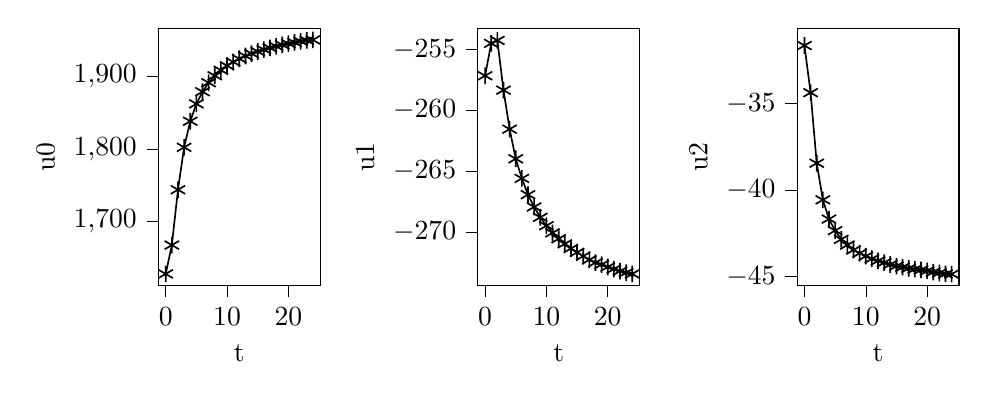
\begin{tikzpicture}

\begin{groupplot}[group style={group size=3 by 1, horizontal sep=2cm, vertical sep=2cm}]
\nextgroupplot[
tick align=outside,
tick pos=left,
x grid style={white!69.0196078431373!black},
xlabel={t},
xmin=-1.2, xmax=25.2,
xtick style={color=black},
y grid style={white!69.0196078431373!black},
ylabel={u0},
ymin=1611.96396507166, ymax=1966.37809243794,
ytick style={color=black},
width=.3\textwidth,
height=.4\textwidth
]
\addplot [semithick, black, mark=asterisk, mark size=3, mark options={solid}]
table {%
0 1628.07369813376
1 1667.71554096531
2 1743.98141797755
3 1802.36425351953
4 1838.30822493671
5 1862.21684026639
6 1878.96158900469
7 1891.36400083709
8 1900.96567861062
9 1908.56716660305
10 1914.77171625286
11 1919.95306705393
12 1924.3277347325
13 1928.10291753782
14 1931.42597796034
15 1934.34704210956
16 1936.92339749995
17 1939.277117136
18 1941.49313059285
19 1943.47640863995
20 1945.22891375994
21 1946.84995604801
22 1948.32295045775
23 1949.64421744529
24 1950.26835937583
};

\nextgroupplot[
tick align=outside,
tick pos=left,
x grid style={white!69.0196078431373!black},
xlabel={t},
xmin=-1.2, xmax=25.2,
xtick style={color=black},
y grid style={white!69.0196078431373!black},
ylabel={u1},
ymin=-274.389309132333, ymax=-253.272398820019,
ytick style={color=black},
width=.3\textwidth,
height=.4\textwidth
]
\addplot [semithick, black, mark=asterisk, mark size=3, mark options={solid}]
table {%
0 -257.171692592497
1 -254.515300494911
2 -254.272398820019
3 -258.351612389057
4 -261.554906914197
5 -263.985260787298
6 -265.594796024212
7 -266.927943185037
8 -267.937156366821
9 -268.78866243541
10 -269.475127597593
11 -270.06335206048
12 -270.548578231464
13 -270.965438493852
14 -271.345643969425
15 -271.665621043199
16 -271.970152853862
17 -272.271974610773
18 -272.505655020541
19 -272.664732264148
20 -272.862874860928
21 -273.036219893531
22 -273.200434711802
23 -273.33315341083
24 -273.431361022223
};

\nextgroupplot[
tick align=outside,
tick pos=left,
x grid style={white!69.0196078431373!black},
xlabel={t},
xmin=-1.2, xmax=25.2,
xtick style={color=black},
y grid style={white!69.0196078431373!black},
ylabel={u2},
ymin=-45.5377536567457, ymax=-30.6623178468017,
ytick style={color=black},
width=.3\textwidth,
height=.4\textwidth
]
\addplot [semithick, black, mark=asterisk, mark size=3, mark options={solid}]
table {%
0 -31.6623178468017
1 -34.3868975136464
2 -38.4638436013163
3 -40.5821733500112
4 -41.6933777077317
5 -42.3578147737184
6 -42.862631832261
7 -43.1940906634818
8 -43.480635907868
9 -43.6672055719659
10 -43.8381580853925
11 -43.9881808121614
12 -44.1065857660735
13 -44.2134327541779
14 -44.3186696834934
15 -44.4117857444969
16 -44.4744224797722
17 -44.5396918879576
18 -44.5871380898455
19 -44.6321316633901
20 -44.6908604463504
21 -44.7588296817474
22 -44.8091704689491
23 -44.8629326044558
24 -44.8770186181769
};
\end{groupplot}

\end{tikzpicture}

	\caption{Characteristic velocities u0, u1, u2 of the code variables var0, var1, var2 respectively calculated as described in \Cref{Reduced Order Model}.}
\end{figure}
\begin{figure}[!htbp]
	% This file was created by tikzplotlib v0.9.6.
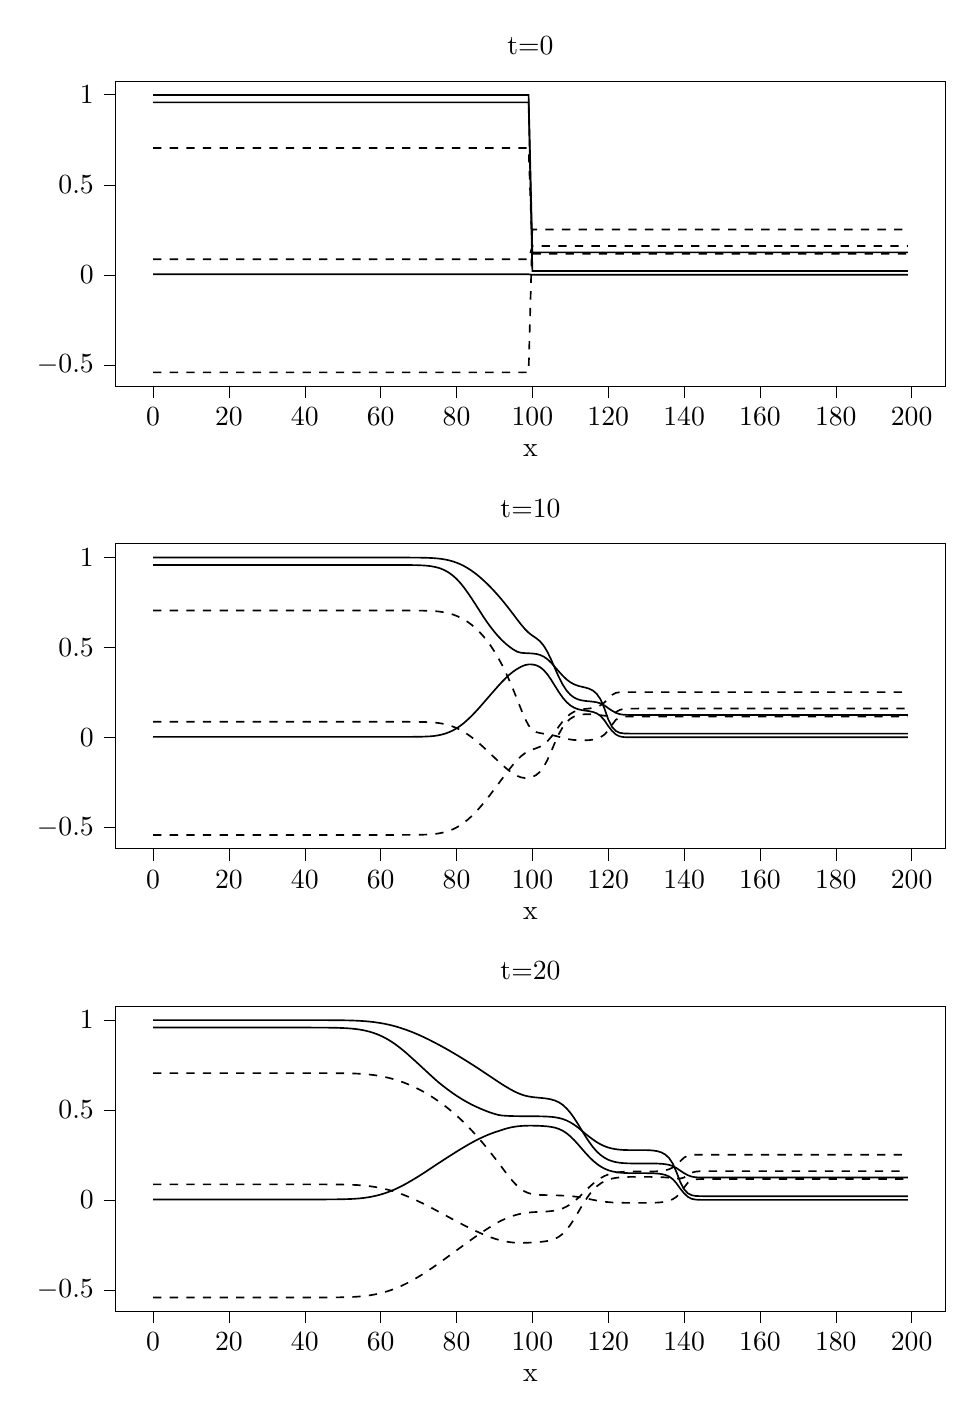
\begin{tikzpicture}

\begin{groupplot}[group style={group size=1 by 3, horizontal sep=2cm, vertical sep=2cm}]
\nextgroupplot[
tick align=outside,
tick pos=left,
title={t=0},
x grid style={white!69.0196078431373!black},
xlabel={x},
xmin=-9.95, xmax=208.95,
xtick style={color=black},
y grid style={white!69.0196078431373!black},
ymin=-0.618888636708649, ymax=1.07585448611601,
ytick style={color=black},
width=\textwidth,
height=.45\textwidth
]
\addplot [semithick, black, dashed]
table {%
0 0.0864763781428337
1 0.0864763781428337
2 0.0864763781428337
3 0.0864763781428337
4 0.0864763781428337
5 0.0864763781428337
6 0.0864763781428337
7 0.0864763781428337
8 0.0864763781428337
9 0.0864763781428337
10 0.0864763781428337
11 0.0864763781428337
12 0.0864763781428337
13 0.0864763781428337
14 0.0864763781428337
15 0.0864763781428337
16 0.0864763781428337
17 0.0864763781428337
18 0.0864763781428337
19 0.0864763781428337
20 0.0864763781428337
21 0.0864763781428337
22 0.0864763781428337
23 0.0864763781428337
24 0.0864763781428337
25 0.0864763781428337
26 0.0864763781428337
27 0.0864763781428337
28 0.0864763781428337
29 0.0864763781428337
30 0.0864763781428337
31 0.0864763781428337
32 0.0864763781428337
33 0.0864763781428337
34 0.0864763781428337
35 0.0864763781428337
36 0.0864763781428337
37 0.0864763781428337
38 0.0864763781428337
39 0.0864763781428337
40 0.0864763781428337
41 0.0864763781428337
42 0.0864763781428337
43 0.0864763781428337
44 0.0864763781428337
45 0.0864763781428337
46 0.0864763781428337
47 0.0864763781428337
48 0.0864763781428337
49 0.0864763781428337
50 0.0864763781428337
51 0.0864763781428337
52 0.0864763781428337
53 0.0864763781428337
54 0.0864763781428337
55 0.0864763781428337
56 0.0864763781428337
57 0.0864763781428337
58 0.0864763781428337
59 0.0864763781428337
60 0.0864763781428337
61 0.0864763781428337
62 0.0864763781428337
63 0.0864763781428337
64 0.0864763781428337
65 0.0864763781428337
66 0.0864763781428337
67 0.0864763781428337
68 0.0864763781428337
69 0.0864763781428337
70 0.0864763781428337
71 0.0864763781428337
72 0.0864763781428337
73 0.0864763781428337
74 0.0864763781428337
75 0.0864763781428337
76 0.0864763781428337
77 0.0864763781428337
78 0.0864763781428337
79 0.0864763781428337
80 0.0864763781428337
81 0.0864763781428337
82 0.0864763781428337
83 0.0864763781428337
84 0.0864763781428337
85 0.0864763781428337
86 0.0864763781428337
87 0.0864763781428337
88 0.0864763781428337
89 0.0864763781428337
90 0.0864763781428337
91 0.0864763781428337
92 0.0864763781428337
93 0.0864763781428337
94 0.0864763781428337
95 0.0864763781428337
96 0.0864763781428337
97 0.0864763781428337
98 0.0864763781428337
99 0.0864763781428337
100 0.159967854619026
101 0.159967854619026
102 0.159967854619026
103 0.159967854619026
104 0.159967854619026
105 0.159967854619026
106 0.159967854619026
107 0.159967854619026
108 0.159967854619026
109 0.159967854619026
110 0.159967854619026
111 0.159967854619026
112 0.159967854619026
113 0.159967854619026
114 0.159967854619026
115 0.159967854619026
116 0.159967854619026
117 0.159967854619026
118 0.159967854619026
119 0.159967854619026
120 0.159967854619026
121 0.159967854619026
122 0.159967854619026
123 0.159967854619026
124 0.159967854619026
125 0.159967854619026
126 0.159967854619026
127 0.159967854619026
128 0.159967854619026
129 0.159967854619026
130 0.159967854619026
131 0.159967854619026
132 0.159967854619026
133 0.159967854619026
134 0.159967854619026
135 0.159967854619026
136 0.159967854619026
137 0.159967854619026
138 0.159967854619026
139 0.159967854619026
140 0.159967854619026
141 0.159967854619026
142 0.159967854619026
143 0.159967854619026
144 0.159967854619026
145 0.159967854619026
146 0.159967854619026
147 0.159967854619026
148 0.159967854619026
149 0.159967854619026
150 0.159967854619026
151 0.159967854619026
152 0.159967854619026
153 0.159967854619026
154 0.159967854619026
155 0.159967854619026
156 0.159967854619026
157 0.159967854619026
158 0.159967854619026
159 0.159967854619026
160 0.159967854619026
161 0.159967854619026
162 0.159967854619026
163 0.159967854619026
164 0.159967854619026
165 0.159967854619026
166 0.159967854619026
167 0.159967854619026
168 0.159967854619026
169 0.159967854619026
170 0.159967854619026
171 0.159967854619026
172 0.159967854619026
173 0.159967854619026
174 0.159967854619026
175 0.159967854619026
176 0.159967854619026
177 0.159967854619026
178 0.159967854619026
179 0.159967854619026
180 0.159967854619026
181 0.159967854619026
182 0.159967854619026
183 0.159967854619026
184 0.159967854619026
185 0.159967854619026
186 0.159967854619026
187 0.159967854619026
188 0.159967854619026
189 0.159967854619026
190 0.159967854619026
191 0.159967854619026
192 0.159967854619026
193 0.159967854619026
194 0.159967854619026
195 0.159967854619026
196 0.159967854619026
197 0.159967854619026
198 0.159967854619026
199 0.159967854619026
};
\addplot [semithick, black]
table {%
0 0.998820707805798
1 0.998820707805798
2 0.998820707805798
3 0.998820707805798
4 0.998820707805798
5 0.998820707805798
6 0.998820707805798
7 0.998820707805798
8 0.998820707805798
9 0.998820707805798
10 0.998820707805798
11 0.998820707805798
12 0.998820707805798
13 0.998820707805798
14 0.998820707805798
15 0.998820707805798
16 0.998820707805798
17 0.998820707805798
18 0.998820707805798
19 0.998820707805798
20 0.998820707805798
21 0.998820707805798
22 0.998820707805798
23 0.998820707805798
24 0.998820707805798
25 0.998820707805798
26 0.998820707805798
27 0.998820707805798
28 0.998820707805798
29 0.998820707805798
30 0.998820707805798
31 0.998820707805798
32 0.998820707805798
33 0.998820707805798
34 0.998820707805798
35 0.998820707805798
36 0.998820707805798
37 0.998820707805798
38 0.998820707805798
39 0.998820707805798
40 0.998820707805798
41 0.998820707805798
42 0.998820707805798
43 0.998820707805798
44 0.998820707805798
45 0.998820707805798
46 0.998820707805798
47 0.998820707805798
48 0.998820707805798
49 0.998820707805798
50 0.998820707805798
51 0.998820707805798
52 0.998820707805798
53 0.998820707805798
54 0.998820707805798
55 0.998820707805798
56 0.998820707805798
57 0.998820707805798
58 0.998820707805798
59 0.998820707805798
60 0.998820707805798
61 0.998820707805798
62 0.998820707805798
63 0.998820707805798
64 0.998820707805798
65 0.998820707805798
66 0.998820707805798
67 0.998820707805798
68 0.998820707805798
69 0.998820707805798
70 0.998820707805798
71 0.998820707805798
72 0.998820707805798
73 0.998820707805798
74 0.998820707805798
75 0.998820707805798
76 0.998820707805798
77 0.998820707805798
78 0.998820707805798
79 0.998820707805798
80 0.998820707805798
81 0.998820707805798
82 0.998820707805798
83 0.998820707805798
84 0.998820707805798
85 0.998820707805798
86 0.998820707805798
87 0.998820707805798
88 0.998820707805798
89 0.998820707805798
90 0.998820707805798
91 0.998820707805798
92 0.998820707805798
93 0.998820707805798
94 0.998820707805798
95 0.998820707805798
96 0.998820707805798
97 0.998820707805798
98 0.998820707805798
99 0.998820707805798
100 0.124468828688082
101 0.124468828688082
102 0.124468828688082
103 0.124468828688082
104 0.124468828688082
105 0.124468828688082
106 0.124468828688082
107 0.124468828688082
108 0.124468828688082
109 0.124468828688082
110 0.124468828688082
111 0.124468828688082
112 0.124468828688082
113 0.124468828688082
114 0.124468828688082
115 0.124468828688082
116 0.124468828688082
117 0.124468828688082
118 0.124468828688082
119 0.124468828688082
120 0.124468828688082
121 0.124468828688082
122 0.124468828688082
123 0.124468828688082
124 0.124468828688082
125 0.124468828688082
126 0.124468828688082
127 0.124468828688082
128 0.124468828688082
129 0.124468828688082
130 0.124468828688082
131 0.124468828688082
132 0.124468828688082
133 0.124468828688082
134 0.124468828688082
135 0.124468828688082
136 0.124468828688082
137 0.124468828688082
138 0.124468828688082
139 0.124468828688082
140 0.124468828688082
141 0.124468828688082
142 0.124468828688082
143 0.124468828688082
144 0.124468828688082
145 0.124468828688082
146 0.124468828688082
147 0.124468828688082
148 0.124468828688082
149 0.124468828688082
150 0.124468828688082
151 0.124468828688082
152 0.124468828688082
153 0.124468828688082
154 0.124468828688082
155 0.124468828688082
156 0.124468828688082
157 0.124468828688082
158 0.124468828688082
159 0.124468828688082
160 0.124468828688082
161 0.124468828688082
162 0.124468828688082
163 0.124468828688082
164 0.124468828688082
165 0.124468828688082
166 0.124468828688082
167 0.124468828688082
168 0.124468828688082
169 0.124468828688082
170 0.124468828688082
171 0.124468828688082
172 0.124468828688082
173 0.124468828688082
174 0.124468828688082
175 0.124468828688082
176 0.124468828688082
177 0.124468828688082
178 0.124468828688082
179 0.124468828688082
180 0.124468828688082
181 0.124468828688082
182 0.124468828688082
183 0.124468828688082
184 0.124468828688082
185 0.124468828688082
186 0.124468828688082
187 0.124468828688082
188 0.124468828688082
189 0.124468828688082
190 0.124468828688082
191 0.124468828688082
192 0.124468828688082
193 0.124468828688082
194 0.124468828688082
195 0.124468828688082
196 0.124468828688082
197 0.124468828688082
198 0.124468828688082
199 0.124468828688082
};
\addplot [semithick, black, dashed]
table {%
0 0.704569160938263
1 0.704569160938263
2 0.704569160938263
3 0.704569160938263
4 0.704569160938263
5 0.704569160938263
6 0.704569160938263
7 0.704569160938263
8 0.704569160938263
9 0.704569160938263
10 0.704569160938263
11 0.704569160938263
12 0.704569160938263
13 0.704569160938263
14 0.704569160938263
15 0.704569160938263
16 0.704569160938263
17 0.704569160938263
18 0.704569160938263
19 0.704569160938263
20 0.704569160938263
21 0.704569160938263
22 0.704569160938263
23 0.704569160938263
24 0.704569160938263
25 0.704569160938263
26 0.704569160938263
27 0.704569160938263
28 0.704569160938263
29 0.704569160938263
30 0.704569160938263
31 0.704569160938263
32 0.704569160938263
33 0.704569160938263
34 0.704569160938263
35 0.704569160938263
36 0.704569160938263
37 0.704569160938263
38 0.704569160938263
39 0.704569160938263
40 0.704569160938263
41 0.704569160938263
42 0.704569160938263
43 0.704569160938263
44 0.704569160938263
45 0.704569160938263
46 0.704569160938263
47 0.704569160938263
48 0.704569160938263
49 0.704569160938263
50 0.704569160938263
51 0.704569160938263
52 0.704569160938263
53 0.704569160938263
54 0.704569160938263
55 0.704569160938263
56 0.704569160938263
57 0.704569160938263
58 0.704569160938263
59 0.704569160938263
60 0.704569160938263
61 0.704569160938263
62 0.704569160938263
63 0.704569160938263
64 0.704569160938263
65 0.704569160938263
66 0.704569160938263
67 0.704569160938263
68 0.704569160938263
69 0.704569160938263
70 0.704569160938263
71 0.704569160938263
72 0.704569160938263
73 0.704569160938263
74 0.704569160938263
75 0.704569160938263
76 0.704569160938263
77 0.704569160938263
78 0.704569160938263
79 0.704569160938263
80 0.704569160938263
81 0.704569160938263
82 0.704569160938263
83 0.704569160938263
84 0.704569160938263
85 0.704569160938263
86 0.704569160938263
87 0.704569160938263
88 0.704569160938263
89 0.704569160938263
90 0.704569160938263
91 0.704569160938263
92 0.704569160938263
93 0.704569160938263
94 0.704569160938263
95 0.704569160938263
96 0.704569160938263
97 0.704569160938263
98 0.704569160938263
99 0.704569160938263
100 0.116299636662006
101 0.116299636662006
102 0.116299636662006
103 0.116299636662006
104 0.116299636662006
105 0.116299636662006
106 0.116299636662006
107 0.116299636662006
108 0.116299636662006
109 0.116299636662006
110 0.116299636662006
111 0.116299636662006
112 0.116299636662006
113 0.116299636662006
114 0.116299636662006
115 0.116299636662006
116 0.116299636662006
117 0.116299636662006
118 0.116299636662006
119 0.116299636662006
120 0.116299636662006
121 0.116299636662006
122 0.116299636662006
123 0.116299636662006
124 0.116299636662006
125 0.116299636662006
126 0.116299636662006
127 0.116299636662006
128 0.116299636662006
129 0.116299636662006
130 0.116299636662006
131 0.116299636662006
132 0.116299636662006
133 0.116299636662006
134 0.116299636662006
135 0.116299636662006
136 0.116299636662006
137 0.116299636662006
138 0.116299636662006
139 0.116299636662006
140 0.116299636662006
141 0.116299636662006
142 0.116299636662006
143 0.116299636662006
144 0.116299636662006
145 0.116299636662006
146 0.116299636662006
147 0.116299636662006
148 0.116299636662006
149 0.116299636662006
150 0.116299636662006
151 0.116299636662006
152 0.116299636662006
153 0.116299636662006
154 0.116299636662006
155 0.116299636662006
156 0.116299636662006
157 0.116299636662006
158 0.116299636662006
159 0.116299636662006
160 0.116299636662006
161 0.116299636662006
162 0.116299636662006
163 0.116299636662006
164 0.116299636662006
165 0.116299636662006
166 0.116299636662006
167 0.116299636662006
168 0.116299636662006
169 0.116299636662006
170 0.116299636662006
171 0.116299636662006
172 0.116299636662006
173 0.116299636662006
174 0.116299636662006
175 0.116299636662006
176 0.116299636662006
177 0.116299636662006
178 0.116299636662006
179 0.116299636662006
180 0.116299636662006
181 0.116299636662006
182 0.116299636662006
183 0.116299636662006
184 0.116299636662006
185 0.116299636662006
186 0.116299636662006
187 0.116299636662006
188 0.116299636662006
189 0.116299636662006
190 0.116299636662006
191 0.116299636662006
192 0.116299636662006
193 0.116299636662006
194 0.116299636662006
195 0.116299636662006
196 0.116299636662006
197 0.116299636662006
198 0.116299636662006
199 0.116299636662006
};
\addplot [semithick, black]
table {%
0 0.957552853847665
1 0.957552853847665
2 0.957552853847665
3 0.957552853847665
4 0.957552853847665
5 0.957552853847665
6 0.957552853847665
7 0.957552853847665
8 0.957552853847665
9 0.957552853847665
10 0.957552853847665
11 0.957552853847665
12 0.957552853847665
13 0.957552853847665
14 0.957552853847665
15 0.957552853847665
16 0.957552853847665
17 0.957552853847665
18 0.957552853847665
19 0.957552853847665
20 0.957552853847665
21 0.957552853847665
22 0.957552853847665
23 0.957552853847665
24 0.957552853847665
25 0.957552853847665
26 0.957552853847665
27 0.957552853847665
28 0.957552853847665
29 0.957552853847665
30 0.957552853847665
31 0.957552853847665
32 0.957552853847665
33 0.957552853847665
34 0.957552853847665
35 0.957552853847665
36 0.957552853847665
37 0.957552853847665
38 0.957552853847665
39 0.957552853847665
40 0.957552853847665
41 0.957552853847665
42 0.957552853847665
43 0.957552853847665
44 0.957552853847665
45 0.957552853847665
46 0.957552853847665
47 0.957552853847665
48 0.957552853847665
49 0.957552853847665
50 0.957552853847665
51 0.957552853847665
52 0.957552853847665
53 0.957552853847665
54 0.957552853847665
55 0.957552853847665
56 0.957552853847665
57 0.957552853847665
58 0.957552853847665
59 0.957552853847665
60 0.957552853847665
61 0.957552853847665
62 0.957552853847665
63 0.957552853847665
64 0.957552853847665
65 0.957552853847665
66 0.957552853847665
67 0.957552853847665
68 0.957552853847665
69 0.957552853847665
70 0.957552853847665
71 0.957552853847665
72 0.957552853847665
73 0.957552853847665
74 0.957552853847665
75 0.957552853847665
76 0.957552853847665
77 0.957552853847665
78 0.957552853847665
79 0.957552853847665
80 0.957552853847665
81 0.957552853847665
82 0.957552853847665
83 0.957552853847665
84 0.957552853847665
85 0.957552853847665
86 0.957552853847665
87 0.957552853847665
88 0.957552853847665
89 0.957552853847665
90 0.957552853847665
91 0.957552853847665
92 0.957552853847665
93 0.957552853847665
94 0.957552853847665
95 0.957552853847665
96 0.957552853847665
97 0.957552853847665
98 0.957552853847665
99 0.957552853847665
100 0.0208907090440876
101 0.0208907090440876
102 0.0208907090440876
103 0.0208907090440876
104 0.0208907090440876
105 0.0208907090440876
106 0.0208907090440876
107 0.0208907090440876
108 0.0208907090440876
109 0.0208907090440876
110 0.0208907090440876
111 0.0208907090440876
112 0.0208907090440876
113 0.0208907090440876
114 0.0208907090440876
115 0.0208907090440876
116 0.0208907090440876
117 0.0208907090440876
118 0.0208907090440876
119 0.0208907090440876
120 0.0208907090440876
121 0.0208907090440876
122 0.0208907090440876
123 0.0208907090440876
124 0.0208907090440876
125 0.0208907090440876
126 0.0208907090440876
127 0.0208907090440876
128 0.0208907090440876
129 0.0208907090440876
130 0.0208907090440876
131 0.0208907090440876
132 0.0208907090440876
133 0.0208907090440876
134 0.0208907090440876
135 0.0208907090440876
136 0.0208907090440876
137 0.0208907090440876
138 0.0208907090440876
139 0.0208907090440876
140 0.0208907090440876
141 0.0208907090440876
142 0.0208907090440876
143 0.0208907090440876
144 0.0208907090440876
145 0.0208907090440876
146 0.0208907090440876
147 0.0208907090440876
148 0.0208907090440876
149 0.0208907090440876
150 0.0208907090440876
151 0.0208907090440876
152 0.0208907090440876
153 0.0208907090440876
154 0.0208907090440876
155 0.0208907090440876
156 0.0208907090440876
157 0.0208907090440876
158 0.0208907090440876
159 0.0208907090440876
160 0.0208907090440876
161 0.0208907090440876
162 0.0208907090440876
163 0.0208907090440876
164 0.0208907090440876
165 0.0208907090440876
166 0.0208907090440876
167 0.0208907090440876
168 0.0208907090440876
169 0.0208907090440876
170 0.0208907090440876
171 0.0208907090440876
172 0.0208907090440876
173 0.0208907090440876
174 0.0208907090440876
175 0.0208907090440876
176 0.0208907090440876
177 0.0208907090440876
178 0.0208907090440876
179 0.0208907090440876
180 0.0208907090440876
181 0.0208907090440876
182 0.0208907090440876
183 0.0208907090440876
184 0.0208907090440876
185 0.0208907090440876
186 0.0208907090440876
187 0.0208907090440876
188 0.0208907090440876
189 0.0208907090440876
190 0.0208907090440876
191 0.0208907090440876
192 0.0208907090440876
193 0.0208907090440876
194 0.0208907090440876
195 0.0208907090440876
196 0.0208907090440876
197 0.0208907090440876
198 0.0208907090440876
199 0.0208907090440876
};
\addplot [semithick, black, dashed]
table {%
0 -0.541854858398438
1 -0.541854858398438
2 -0.541854858398438
3 -0.541854858398438
4 -0.541854858398438
5 -0.541854858398438
6 -0.541854858398438
7 -0.541854858398438
8 -0.541854858398438
9 -0.541854858398438
10 -0.541854858398438
11 -0.541854858398438
12 -0.541854858398438
13 -0.541854858398438
14 -0.541854858398438
15 -0.541854858398438
16 -0.541854858398438
17 -0.541854858398438
18 -0.541854858398438
19 -0.541854858398438
20 -0.541854858398438
21 -0.541854858398438
22 -0.541854858398438
23 -0.541854858398438
24 -0.541854858398438
25 -0.541854858398438
26 -0.541854858398438
27 -0.541854858398438
28 -0.541854858398438
29 -0.541854858398438
30 -0.541854858398438
31 -0.541854858398438
32 -0.541854858398438
33 -0.541854858398438
34 -0.541854858398438
35 -0.541854858398438
36 -0.541854858398438
37 -0.541854858398438
38 -0.541854858398438
39 -0.541854858398438
40 -0.541854858398438
41 -0.541854858398438
42 -0.541854858398438
43 -0.541854858398438
44 -0.541854858398438
45 -0.541854858398438
46 -0.541854858398438
47 -0.541854858398438
48 -0.541854858398438
49 -0.541854858398438
50 -0.541854858398438
51 -0.541854858398438
52 -0.541854858398438
53 -0.541854858398438
54 -0.541854858398438
55 -0.541854858398438
56 -0.541854858398438
57 -0.541854858398438
58 -0.541854858398438
59 -0.541854858398438
60 -0.541854858398438
61 -0.541854858398438
62 -0.541854858398438
63 -0.541854858398438
64 -0.541854858398438
65 -0.541854858398438
66 -0.541854858398438
67 -0.541854858398438
68 -0.541854858398438
69 -0.541854858398438
70 -0.541854858398438
71 -0.541854858398438
72 -0.541854858398438
73 -0.541854858398438
74 -0.541854858398438
75 -0.541854858398438
76 -0.541854858398438
77 -0.541854858398438
78 -0.541854858398438
79 -0.541854858398438
80 -0.541854858398438
81 -0.541854858398438
82 -0.541854858398438
83 -0.541854858398438
84 -0.541854858398438
85 -0.541854858398438
86 -0.541854858398438
87 -0.541854858398438
88 -0.541854858398438
89 -0.541854858398438
90 -0.541854858398438
91 -0.541854858398438
92 -0.541854858398438
93 -0.541854858398438
94 -0.541854858398438
95 -0.541854858398438
96 -0.541854858398438
97 -0.541854858398438
98 -0.541854858398438
99 -0.541854858398438
100 0.251547485589981
101 0.251547485589981
102 0.251547485589981
103 0.251547485589981
104 0.251547485589981
105 0.251547485589981
106 0.251547485589981
107 0.251547485589981
108 0.251547485589981
109 0.251547485589981
110 0.251547485589981
111 0.251547485589981
112 0.251547485589981
113 0.251547485589981
114 0.251547485589981
115 0.251547485589981
116 0.251547485589981
117 0.251547485589981
118 0.251547485589981
119 0.251547485589981
120 0.251547485589981
121 0.251547485589981
122 0.251547485589981
123 0.251547485589981
124 0.251547485589981
125 0.251547485589981
126 0.251547485589981
127 0.251547485589981
128 0.251547485589981
129 0.251547485589981
130 0.251547485589981
131 0.251547485589981
132 0.251547485589981
133 0.251547485589981
134 0.251547485589981
135 0.251547485589981
136 0.251547485589981
137 0.251547485589981
138 0.251547485589981
139 0.251547485589981
140 0.251547485589981
141 0.251547485589981
142 0.251547485589981
143 0.251547485589981
144 0.251547485589981
145 0.251547485589981
146 0.251547485589981
147 0.251547485589981
148 0.251547485589981
149 0.251547485589981
150 0.251547485589981
151 0.251547485589981
152 0.251547485589981
153 0.251547485589981
154 0.251547485589981
155 0.251547485589981
156 0.251547485589981
157 0.251547485589981
158 0.251547485589981
159 0.251547485589981
160 0.251547485589981
161 0.251547485589981
162 0.251547485589981
163 0.251547485589981
164 0.251547485589981
165 0.251547485589981
166 0.251547485589981
167 0.251547485589981
168 0.251547485589981
169 0.251547485589981
170 0.251547485589981
171 0.251547485589981
172 0.251547485589981
173 0.251547485589981
174 0.251547485589981
175 0.251547485589981
176 0.251547485589981
177 0.251547485589981
178 0.251547485589981
179 0.251547485589981
180 0.251547485589981
181 0.251547485589981
182 0.251547485589981
183 0.251547485589981
184 0.251547485589981
185 0.251547485589981
186 0.251547485589981
187 0.251547485589981
188 0.251547485589981
189 0.251547485589981
190 0.251547485589981
191 0.251547485589981
192 0.251547485589981
193 0.251547485589981
194 0.251547485589981
195 0.251547485589981
196 0.251547485589981
197 0.251547485589981
198 0.251547485589981
199 0.251547485589981
};
\addplot [semithick, black]
table {%
0 0.00276484748660005
1 0.00276484748660005
2 0.00276484748660005
3 0.00276484748660005
4 0.00276484748660005
5 0.00276484748660005
6 0.00276484748660005
7 0.00276484748660005
8 0.00276484748660005
9 0.00276484748660005
10 0.00276484748660005
11 0.00276484748660005
12 0.00276484748660005
13 0.00276484748660005
14 0.00276484748660005
15 0.00276484748660005
16 0.00276484748660005
17 0.00276484748660005
18 0.00276484748660005
19 0.00276484748660005
20 0.00276484748660005
21 0.00276484748660005
22 0.00276484748660005
23 0.00276484748660005
24 0.00276484748660005
25 0.00276484748660005
26 0.00276484748660005
27 0.00276484748660005
28 0.00276484748660005
29 0.00276484748660005
30 0.00276484748660005
31 0.00276484748660005
32 0.00276484748660005
33 0.00276484748660005
34 0.00276484748660005
35 0.00276484748660005
36 0.00276484748660005
37 0.00276484748660005
38 0.00276484748660005
39 0.00276484748660005
40 0.00276484748660005
41 0.00276484748660005
42 0.00276484748660005
43 0.00276484748660005
44 0.00276484748660005
45 0.00276484748660005
46 0.00276484748660005
47 0.00276484748660005
48 0.00276484748660005
49 0.00276484748660005
50 0.00276484748660005
51 0.00276484748660005
52 0.00276484748660005
53 0.00276484748660005
54 0.00276484748660005
55 0.00276484748660005
56 0.00276484748660005
57 0.00276484748660005
58 0.00276484748660005
59 0.00276484748660005
60 0.00276484748660005
61 0.00276484748660005
62 0.00276484748660005
63 0.00276484748660005
64 0.00276484748660005
65 0.00276484748660005
66 0.00276484748660005
67 0.00276484748660005
68 0.00276484748660005
69 0.00276484748660005
70 0.00276484748660005
71 0.00276484748660005
72 0.00276484748660005
73 0.00276484748660005
74 0.00276484748660005
75 0.00276484748660005
76 0.00276484748660005
77 0.00276484748660005
78 0.00276484748660005
79 0.00276484748660005
80 0.00276484748660005
81 0.00276484748660005
82 0.00276484748660005
83 0.00276484748660005
84 0.00276484748660005
85 0.00276484748660005
86 0.00276484748660005
87 0.00276484748660005
88 0.00276484748660005
89 0.00276484748660005
90 0.00276484748660005
91 0.00276484748660005
92 0.00276484748660005
93 0.00276484748660005
94 0.00276484748660005
95 0.00276484748660005
96 0.00276484748660005
97 0.00276484748660005
98 0.00276484748660005
99 0.00276484748660005
100 0.000327279684018397
101 0.000327279684018397
102 0.000327279684018397
103 0.000327279684018397
104 0.000327279684018397
105 0.000327279684018397
106 0.000327279684018397
107 0.000327279684018397
108 0.000327279684018397
109 0.000327279684018397
110 0.000327279684018397
111 0.000327279684018397
112 0.000327279684018397
113 0.000327279684018397
114 0.000327279684018397
115 0.000327279684018397
116 0.000327279684018397
117 0.000327279684018397
118 0.000327279684018397
119 0.000327279684018397
120 0.000327279684018397
121 0.000327279684018397
122 0.000327279684018397
123 0.000327279684018397
124 0.000327279684018397
125 0.000327279684018397
126 0.000327279684018397
127 0.000327279684018397
128 0.000327279684018397
129 0.000327279684018397
130 0.000327279684018397
131 0.000327279684018397
132 0.000327279684018397
133 0.000327279684018397
134 0.000327279684018397
135 0.000327279684018397
136 0.000327279684018397
137 0.000327279684018397
138 0.000327279684018397
139 0.000327279684018397
140 0.000327279684018397
141 0.000327279684018397
142 0.000327279684018397
143 0.000327279684018397
144 0.000327279684018397
145 0.000327279684018397
146 0.000327279684018397
147 0.000327279684018397
148 0.000327279684018397
149 0.000327279684018397
150 0.000327279684018397
151 0.000327279684018397
152 0.000327279684018397
153 0.000327279684018397
154 0.000327279684018397
155 0.000327279684018397
156 0.000327279684018397
157 0.000327279684018397
158 0.000327279684018397
159 0.000327279684018397
160 0.000327279684018397
161 0.000327279684018397
162 0.000327279684018397
163 0.000327279684018397
164 0.000327279684018397
165 0.000327279684018397
166 0.000327279684018397
167 0.000327279684018397
168 0.000327279684018397
169 0.000327279684018397
170 0.000327279684018397
171 0.000327279684018397
172 0.000327279684018397
173 0.000327279684018397
174 0.000327279684018397
175 0.000327279684018397
176 0.000327279684018397
177 0.000327279684018397
178 0.000327279684018397
179 0.000327279684018397
180 0.000327279684018397
181 0.000327279684018397
182 0.000327279684018397
183 0.000327279684018397
184 0.000327279684018397
185 0.000327279684018397
186 0.000327279684018397
187 0.000327279684018397
188 0.000327279684018397
189 0.000327279684018397
190 0.000327279684018397
191 0.000327279684018397
192 0.000327279684018397
193 0.000327279684018397
194 0.000327279684018397
195 0.000327279684018397
196 0.000327279684018397
197 0.000327279684018397
198 0.000327279684018397
199 0.000327279684018397
};

\nextgroupplot[
tick align=outside,
tick pos=left,
title={t=10},
x grid style={white!69.0196078431373!black},
xlabel={x},
xmin=-9.95, xmax=208.95,
xtick style={color=black},
y grid style={white!69.0196078431373!black},
ymin=-0.618888640008754, ymax=1.0758545554182,
ytick style={color=black},
width=\textwidth,
height=.45\textwidth
]
\addplot [semithick, black, dashed]
table {%
0 0.0864763781428337
1 0.0864763781428337
2 0.0864763781428337
3 0.0864763781428337
4 0.0864763781428337
5 0.0864763781428337
6 0.0864763781428337
7 0.0864763781428337
8 0.0864763781428337
9 0.0864763781428337
10 0.0864763781428337
11 0.0864763781428337
12 0.0864763781428337
13 0.0864763781428337
14 0.0864763781428337
15 0.0864763781428337
16 0.0864763781428337
17 0.0864763781428337
18 0.0864763781428337
19 0.0864763781428337
20 0.0864763781428337
21 0.0864763781428337
22 0.0864763781428337
23 0.0864763781428337
24 0.0864763781428337
25 0.0864763781428337
26 0.0864763781428337
27 0.0864763781428337
28 0.0864763781428337
29 0.0864763781428337
30 0.0864763781428337
31 0.0864763781428337
32 0.0864763781428337
33 0.0864763781428337
34 0.0864763781428337
35 0.0864763781428337
36 0.0864763781428337
37 0.0864763781428337
38 0.0864763781428337
39 0.0864763781428337
40 0.0864763781428337
41 0.0864763781428337
42 0.0864763781428337
43 0.0864763781428337
44 0.0864763781428337
45 0.0864763781428337
46 0.0864763781428337
47 0.0864763781428337
48 0.0864763781428337
49 0.0864763781428337
50 0.0864763781428337
51 0.0864763781428337
52 0.0864763781428337
53 0.0864763781428337
54 0.0864763781428337
55 0.0864763781428337
56 0.0864763706922531
57 0.0864763334393501
58 0.0864762738347054
59 0.0864761620759964
60 0.0864758640527725
61 0.0864753127098083
62 0.0864739865064621
63 0.0864712372422218
64 0.0864655897021294
65 0.0864543095231056
66 0.0864325016736984
67 0.0863915756344795
68 0.0863169431686401
69 0.0861852243542671
70 0.0859597772359848
71 0.0855867117643356
72 0.0849898457527161
73 0.0840671584010124
74 0.0826498940587044
75 0.0803875625133514
76 0.077234223484993
77 0.072984017431736
78 0.0674387067556381
79 0.0604246556758881
80 0.0518089793622494
81 0.0415117479860783
82 0.0295130852609873
83 0.0158548932522535
84 0.0006373300566338
85 -0.015987241640687
86 -0.0338233225047588
87 -0.0526409223675728
88 -0.07218337059021
89 -0.0921719744801521
90 -0.112306721508503
91 -0.132261112332344
92 -0.151669800281525
93 -0.170107528567314
94 -0.187061071395874
95 -0.20189805328846
96 -0.21385258436203
97 -0.222053498029709
98 -0.225772872567177
99 -0.224780276417732
100 -0.219312369823456
101 -0.209041133522987
102 -0.191329523921013
103 -0.163140207529068
104 -0.123704329133034
105 -0.076011136174202
106 -0.0262000784277916
107 0.0194125380367041
108 0.0566670969128609
109 0.0843709632754326
110 0.103447303175926
111 0.115707568824291
112 0.123025268316269
113 0.126965016126633
114 0.128674626350403
115 0.128887668251991
116 0.127975702285767
117 0.126061379909515
118 0.123282037675381
119 0.120394363999367
120 0.119689486920834
121 0.125713557004929
122 0.139865666627884
123 0.152246356010437
124 0.157710343599319
125 0.159378811717033
126 0.1598189920187
127 0.159929275512695
128 0.159956306219101
129 0.159962862730026
130 0.159964442253113
131 0.159964799880981
132 0.159964889287949
133 0.159964919090271
134 0.159964919090271
135 0.159964919090271
136 0.159964919090271
137 0.159964919090271
138 0.159964919090271
139 0.159964919090271
140 0.159964919090271
141 0.159964919090271
142 0.159964919090271
143 0.159964919090271
144 0.159964919090271
145 0.159964919090271
146 0.159964919090271
147 0.159964919090271
148 0.159964919090271
149 0.159964919090271
150 0.159964919090271
151 0.159964919090271
152 0.159964919090271
153 0.159964919090271
154 0.159964919090271
155 0.159964919090271
156 0.159964919090271
157 0.159964919090271
158 0.159964919090271
159 0.159964919090271
160 0.159964919090271
161 0.159964919090271
162 0.159964919090271
163 0.159964919090271
164 0.159964919090271
165 0.159964919090271
166 0.159964919090271
167 0.159964919090271
168 0.159964919090271
169 0.159964919090271
170 0.159964919090271
171 0.159964919090271
172 0.159964919090271
173 0.159964919090271
174 0.159964919090271
175 0.159964919090271
176 0.159964919090271
177 0.159964919090271
178 0.159964919090271
179 0.159964919090271
180 0.159964919090271
181 0.159964919090271
182 0.159964919090271
183 0.159964919090271
184 0.159964919090271
185 0.159964919090271
186 0.159964919090271
187 0.159964919090271
188 0.159964919090271
189 0.159964919090271
190 0.159964919090271
191 0.159964919090271
192 0.159964919090271
193 0.159964919090271
194 0.159964919090271
195 0.159964919090271
196 0.159964919090271
197 0.159964919090271
198 0.159964919090271
199 0.159964919090271
};
\addplot [semithick, black]
table {%
0 0.998820707805798
1 0.998820707805798
2 0.998820707805798
3 0.998820707805798
4 0.998820707805798
5 0.998820707805798
6 0.998820707805798
7 0.998820707805798
8 0.998820707805798
9 0.998820707805798
10 0.998820707805798
11 0.998820707805798
12 0.998820707805798
13 0.998820707805798
14 0.998820707805798
15 0.998820707805798
16 0.998820707805798
17 0.998820707805798
18 0.998820707805798
19 0.998820707805798
20 0.998820707805798
21 0.998820707805798
22 0.998820707805798
23 0.998820707805798
24 0.998820707805798
25 0.998820707805798
26 0.998820707805798
27 0.998820707805798
28 0.998820707805798
29 0.998820707805798
30 0.998820707805798
31 0.998820707805798
32 0.998820707805798
33 0.998820707805798
34 0.998820707805798
35 0.998820707805798
36 0.998820707805798
37 0.998820707805798
38 0.998820707805798
39 0.998820707805798
40 0.998820707805798
41 0.998820707805798
42 0.998820707805798
43 0.998820707805798
44 0.998820707805798
45 0.998820707805798
46 0.998820707805798
47 0.998820707805798
48 0.998820707805798
49 0.998820707805798
50 0.998820707805798
51 0.998820707805798
52 0.998820707805798
53 0.998820707805798
54 0.998820707805798
55 0.998820707805798
56 0.998820760291134
57 0.998820773807887
58 0.998820724033428
59 0.998820498134271
60 0.998820354072147
61 0.998819787491957
62 0.998818709993266
63 0.998816438867519
64 0.998811647653366
65 0.998802133932894
66 0.998783784556689
67 0.998749135413204
68 0.998685901983972
69 0.998573943772108
70 0.998382093047095
71 0.99806367534647
72 0.99755233596683
73 0.996758791228966
74 0.995562235864764
75 0.993795790222888
76 0.991312451792947
77 0.987930607509993
78 0.983461891827346
79 0.977723691639446
80 0.970549134859547
81 0.96179809916837
82 0.951367633436214
83 0.939189634603496
84 0.925419590008629
85 0.910015075847446
86 0.892986014455346
87 0.874414008147095
88 0.854575300913485
89 0.833530392317826
90 0.811196551657047
91 0.787644835338538
92 0.762925393836877
93 0.737093863691496
94 0.710239872576506
95 0.682530534706518
96 0.654519607214052
97 0.627513133201249
98 0.602692004498784
99 0.581505205990745
100 0.564988579789525
101 0.551121995186361
102 0.534104219966768
103 0.508901579789661
104 0.473503964586155
105 0.429484190838663
106 0.380857970886953
107 0.333951645265281
108 0.293033010955941
109 0.260566858589113
110 0.236948914774378
111 0.221048299986834
112 0.211176159217967
113 0.205497573825153
114 0.202345116911322
115 0.200305667236441
116 0.198136378712661
117 0.194655276853458
118 0.188450423047004
119 0.177507850479136
120 0.162286801397642
121 0.14817348059739
122 0.136511400662351
123 0.129026887965
124 0.125828234000402
125 0.124826781878442
126 0.124558060439283
127 0.124490321391897
128 0.124473699448391
129 0.124469624696705
130 0.124468652921643
131 0.124468480856789
132 0.124468422541854
133 0.124468384792402
134 0.124468384792402
135 0.124468384792402
136 0.124468384792402
137 0.124468384792402
138 0.124468384792402
139 0.124468384792402
140 0.124468384792402
141 0.124468384792402
142 0.124468384792402
143 0.124468384792402
144 0.124468384792402
145 0.124468384792402
146 0.124468384792402
147 0.124468384792402
148 0.124468384792402
149 0.124468384792402
150 0.124468384792402
151 0.124468384792402
152 0.124468384792402
153 0.124468384792402
154 0.124468384792402
155 0.124468384792402
156 0.124468384792402
157 0.124468384792402
158 0.124468384792402
159 0.124468384792402
160 0.124468384792402
161 0.124468384792402
162 0.124468384792402
163 0.124468384792402
164 0.124468384792402
165 0.124468384792402
166 0.124468384792402
167 0.124468384792402
168 0.124468384792402
169 0.124468384792402
170 0.124468384792402
171 0.124468384792402
172 0.124468384792402
173 0.124468384792402
174 0.124468384792402
175 0.124468384792402
176 0.124468384792402
177 0.124468384792402
178 0.124468384792402
179 0.124468384792402
180 0.124468384792402
181 0.124468384792402
182 0.124468384792402
183 0.124468384792402
184 0.124468384792402
185 0.124468384792402
186 0.124468384792402
187 0.124468384792402
188 0.124468384792402
189 0.124468384792402
190 0.124468384792402
191 0.124468384792402
192 0.124468384792402
193 0.124468384792402
194 0.124468384792402
195 0.124468384792402
196 0.124468384792402
197 0.124468384792402
198 0.124468384792402
199 0.124468384792402
};
\addplot [semithick, black, dashed]
table {%
0 0.704569160938263
1 0.704569160938263
2 0.704569160938263
3 0.704569160938263
4 0.704569160938263
5 0.704569160938263
6 0.704569160938263
7 0.704569160938263
8 0.704569160938263
9 0.704569160938263
10 0.704569160938263
11 0.704569160938263
12 0.704569160938263
13 0.704569160938263
14 0.704569160938263
15 0.704569160938263
16 0.704569160938263
17 0.704569160938263
18 0.704569160938263
19 0.704569160938263
20 0.704569160938263
21 0.704569160938263
22 0.704569160938263
23 0.704569160938263
24 0.704569160938263
25 0.704569160938263
26 0.704569160938263
27 0.704569160938263
28 0.704569160938263
29 0.704569160938263
30 0.704569160938263
31 0.704569160938263
32 0.704569160938263
33 0.704569160938263
34 0.704569160938263
35 0.704569160938263
36 0.704569160938263
37 0.704569160938263
38 0.704569160938263
39 0.704569160938263
40 0.704569160938263
41 0.704569160938263
42 0.704569160938263
43 0.704569160938263
44 0.704569160938263
45 0.704569160938263
46 0.704569160938263
47 0.704569160938263
48 0.704569160938263
49 0.704569160938263
50 0.704569160938263
51 0.704569160938263
52 0.704569160938263
53 0.704569160938263
54 0.704569160938263
55 0.704569160938263
56 0.704569160938263
57 0.704569160938263
58 0.704569160938263
59 0.704568982124329
60 0.704568862915039
61 0.704568445682526
62 0.704567492008209
63 0.704565465450287
64 0.704561412334442
65 0.704553306102753
66 0.704537510871887
67 0.704507768154144
68 0.704453468322754
69 0.704357147216797
70 0.7041916847229
71 0.703916788101196
72 0.703474700450897
73 0.702787220478058
74 0.701700329780579
75 0.699823677539825
76 0.697181940078735
77 0.693577826023102
78 0.688804566860199
79 0.682656288146973
80 0.674936413764954
81 0.665463805198669
82 0.654076278209686
83 0.640629291534424
84 0.624991059303284
85 0.607034862041473
86 0.58662885427475
87 0.563625574111938
88 0.537850975990295
89 0.509098589420319
90 0.477130085229874
91 0.441690415143967
92 0.402544021606445
93 0.359548419713974
94 0.312781065702438
95 0.262749254703522
96 0.210713937878609
97 0.156980127096176
98 0.106523342430592
99 0.0665870159864426
100 0.0413695275783539
101 0.0293617248535156
102 0.0239757392555475
103 0.020589392632246
104 0.017328942194581
105 0.0135651845484972
106 0.00868136994540691
107 0.00309600448235869
108 -0.0026007981505245
109 -0.00770871713757515
110 -0.0117128798738122
111 -0.0144491270184517
112 -0.0160266142338514
113 -0.0166347697377205
114 -0.0163671504706144
115 -0.0150983184576035
116 -0.0123885935172439
117 -0.00738534331321716
118 0.00128830154426396
119 0.0155978444963694
120 0.0383731126785278
121 0.069693423807621
122 0.0973233729600906
123 0.110729277133942
124 0.114920169115067
125 0.115955129265785
126 0.116202712059021
127 0.116262666881084
128 0.116277255117893
129 0.116280786693096
130 0.116281636059284
131 0.116281822323799
132 0.116281874477863
133 0.116281881928444
134 0.116281881928444
135 0.116281881928444
136 0.116281881928444
137 0.116281881928444
138 0.116281881928444
139 0.116281881928444
140 0.116281881928444
141 0.116281881928444
142 0.116281881928444
143 0.116281881928444
144 0.116281881928444
145 0.116281881928444
146 0.116281881928444
147 0.116281881928444
148 0.116281881928444
149 0.116281881928444
150 0.116281881928444
151 0.116281881928444
152 0.116281881928444
153 0.116281881928444
154 0.116281881928444
155 0.116281881928444
156 0.116281881928444
157 0.116281881928444
158 0.116281881928444
159 0.116281881928444
160 0.116281881928444
161 0.116281881928444
162 0.116281881928444
163 0.116281881928444
164 0.116281881928444
165 0.116281881928444
166 0.116281881928444
167 0.116281881928444
168 0.116281881928444
169 0.116281881928444
170 0.116281881928444
171 0.116281881928444
172 0.116281881928444
173 0.116281881928444
174 0.116281881928444
175 0.116281881928444
176 0.116281881928444
177 0.116281881928444
178 0.116281881928444
179 0.116281881928444
180 0.116281881928444
181 0.116281881928444
182 0.116281881928444
183 0.116281881928444
184 0.116281881928444
185 0.116281881928444
186 0.116281881928444
187 0.116281881928444
188 0.116281881928444
189 0.116281881928444
190 0.116281881928444
191 0.116281881928444
192 0.116281881928444
193 0.116281881928444
194 0.116281881928444
195 0.116281881928444
196 0.116281881928444
197 0.116281881928444
198 0.116281881928444
199 0.116281881928444
};
\addplot [semithick, black]
table {%
0 0.957552853847665
1 0.957552853847665
2 0.957552853847665
3 0.957552853847665
4 0.957552853847665
5 0.957552853847665
6 0.957552853847665
7 0.957552853847665
8 0.957552853847665
9 0.957552853847665
10 0.957552853847665
11 0.957552853847665
12 0.957552853847665
13 0.957552853847665
14 0.957552853847665
15 0.957552853847665
16 0.957552853847665
17 0.957552853847665
18 0.957552853847665
19 0.957552853847665
20 0.957552853847665
21 0.957552853847665
22 0.957552853847665
23 0.957552853847665
24 0.957552853847665
25 0.957552853847665
26 0.957552853847665
27 0.957552853847665
28 0.957552853847665
29 0.957552853847665
30 0.957552853847665
31 0.957552853847665
32 0.957552853847665
33 0.957552853847665
34 0.957552853847665
35 0.957552853847665
36 0.957552853847665
37 0.957552853847665
38 0.957552853847665
39 0.957552853847665
40 0.957552853847665
41 0.957552853847665
42 0.957552853847665
43 0.957552853847665
44 0.957552853847665
45 0.957552853847665
46 0.957552853847665
47 0.957552853847665
48 0.957552853847665
49 0.957552853847665
50 0.957552853847665
51 0.957552853847665
52 0.957552853847665
53 0.957552853847665
54 0.957552853847665
55 0.957552853847665
56 0.957553070479872
57 0.957552965422413
58 0.957552901090213
59 0.957552550484429
60 0.957551652736035
61 0.957550141846559
62 0.957546885167275
63 0.957540536687994
64 0.957526364649298
65 0.957498698893319
66 0.957445017450037
67 0.957344257306809
68 0.957160034496693
69 0.956835113573767
70 0.956278716724211
71 0.955357520571329
72 0.953881476752329
73 0.951598339721755
74 0.948180256377984
75 0.943222931178703
76 0.936304445644686
77 0.926969393556305
78 0.914776651315321
79 0.899346346654798
80 0.880395247441065
81 0.857776648635739
82 0.83167004977711
83 0.802193504629856
84 0.771308436993083
85 0.739013760376995
86 0.705985825271701
87 0.672750046428961
88 0.641530501807081
89 0.612810348899291
90 0.585920215853186
91 0.561337710979005
92 0.53929451043693
93 0.519815610552971
94 0.502700954885152
95 0.487717231624925
96 0.475888690200626
97 0.469924371045881
98 0.468154474119208
99 0.467193815366937
100 0.466021381474596
101 0.463437548448543
102 0.458034584957599
103 0.44841713540577
104 0.433675763289197
105 0.413782152716962
106 0.389244473934469
107 0.365625593486422
108 0.342453341479319
109 0.322186345162689
110 0.306310064399753
111 0.294653337974666
112 0.286722965511438
113 0.281258162708101
114 0.276508001171003
115 0.270265397899795
116 0.259626879459796
117 0.241082289224233
118 0.210082795957879
119 0.160159442835277
120 0.100065189291374
121 0.0584171311146538
122 0.0355787553936021
123 0.025521040255237
124 0.0221560387065928
125 0.0212178854943656
126 0.020976568817763
127 0.0209165328234194
128 0.0209018680157167
129 0.0208982807268322
130 0.0208973653619861
131 0.0208972316128896
132 0.0208971837108023
133 0.0208971605805275
134 0.0208971605805275
135 0.0208971605805275
136 0.0208971605805275
137 0.0208971605805275
138 0.0208971605805275
139 0.0208971605805275
140 0.0208971605805275
141 0.0208971605805275
142 0.0208971605805275
143 0.0208971605805275
144 0.0208971605805275
145 0.0208971605805275
146 0.0208971605805275
147 0.0208971605805275
148 0.0208971605805275
149 0.0208971605805275
150 0.0208971605805275
151 0.0208971605805275
152 0.0208971605805275
153 0.0208971605805275
154 0.0208971605805275
155 0.0208971605805275
156 0.0208971605805275
157 0.0208971605805275
158 0.0208971605805275
159 0.0208971605805275
160 0.0208971605805275
161 0.0208971605805275
162 0.0208971605805275
163 0.0208971605805275
164 0.0208971605805275
165 0.0208971605805275
166 0.0208971605805275
167 0.0208971605805275
168 0.0208971605805275
169 0.0208971605805275
170 0.0208971605805275
171 0.0208971605805275
172 0.0208971605805275
173 0.0208971605805275
174 0.0208971605805275
175 0.0208971605805275
176 0.0208971605805275
177 0.0208971605805275
178 0.0208971605805275
179 0.0208971605805275
180 0.0208971605805275
181 0.0208971605805275
182 0.0208971605805275
183 0.0208971605805275
184 0.0208971605805275
185 0.0208971605805275
186 0.0208971605805275
187 0.0208971605805275
188 0.0208971605805275
189 0.0208971605805275
190 0.0208971605805275
191 0.0208971605805275
192 0.0208971605805275
193 0.0208971605805275
194 0.0208971605805275
195 0.0208971605805275
196 0.0208971605805275
197 0.0208971605805275
198 0.0208971605805275
199 0.0208971605805275
};
\addplot [semithick, black, dashed]
table {%
0 -0.541854858398438
1 -0.541854858398438
2 -0.541854858398438
3 -0.541854858398438
4 -0.541854858398438
5 -0.541854858398438
6 -0.541854858398438
7 -0.541854858398438
8 -0.541854858398438
9 -0.541854858398438
10 -0.541854858398438
11 -0.541854858398438
12 -0.541854858398438
13 -0.541854858398438
14 -0.541854858398438
15 -0.541854858398438
16 -0.541854858398438
17 -0.541854858398438
18 -0.541854858398438
19 -0.541854858398438
20 -0.541854858398438
21 -0.541854858398438
22 -0.541854858398438
23 -0.541854858398438
24 -0.541854858398438
25 -0.541854858398438
26 -0.541854858398438
27 -0.541854858398438
28 -0.541854858398438
29 -0.541854858398438
30 -0.541854858398438
31 -0.541854858398438
32 -0.541854858398438
33 -0.541854858398438
34 -0.541854858398438
35 -0.541854858398438
36 -0.541854858398438
37 -0.541854858398438
38 -0.541854858398438
39 -0.541854858398438
40 -0.541854858398438
41 -0.541854858398438
42 -0.541854858398438
43 -0.541854858398438
44 -0.541854858398438
45 -0.541854858398438
46 -0.541854858398438
47 -0.541854858398438
48 -0.541854858398438
49 -0.541854858398438
50 -0.541854858398438
51 -0.541854858398438
52 -0.541854858398438
53 -0.541854858398438
54 -0.541854858398438
55 -0.541854858398438
56 -0.541854858398438
57 -0.541854858398438
58 -0.541854798793793
59 -0.541854619979858
60 -0.541854321956635
61 -0.541853606700897
62 -0.541851878166199
63 -0.541848480701447
64 -0.541841387748718
65 -0.541827321052551
66 -0.541799962520599
67 -0.541748642921448
68 -0.541655004024506
69 -0.54148942232132
70 -0.541205883026123
71 -0.540736138820648
72 -0.53998327255249
73 -0.538817286491394
74 -0.537055909633636
75 -0.534419476985931
76 -0.530730426311493
77 -0.525734603404999
78 -0.519178509712219
79 -0.510827898979187
80 -0.500485718250275
81 -0.488007426261902
82 -0.473311334848404
83 -0.456383794546127
84 -0.437280178070068
85 -0.416120678186417
86 -0.393084168434143
87 -0.368399024009705
88 -0.342333793640137
89 -0.315187960863113
90 -0.287284761667252
91 -0.258967310190201
92 -0.230598509311676
93 -0.202567085623741
94 -0.17530132830143
95 -0.149292126297951
96 -0.125130087137222
97 -0.104794256389141
98 -0.0885848701000214
99 -0.0761684700846672
100 -0.0673421174287796
101 -0.0603746809065342
102 -0.0519130416214466
103 -0.0391237176954746
104 -0.0205994900316
105 0.00341476663015783
106 0.0317355617880821
107 0.061243761330843
108 0.0888773947954178
109 0.11224415153265
110 0.13013768196106
111 0.142596229910851
112 0.150535672903061
113 0.155268877744675
114 0.158165469765663
115 0.160528555512428
116 0.163659483194351
117 0.16904704272747
118 0.178551405668259
119 0.194100067019463
120 0.21522419154644
121 0.235594436526299
122 0.247201696038246
123 0.25044921040535
124 0.251256018877029
125 0.251471012830734
126 0.251527220010757
127 0.251541405916214
128 0.251544862985611
129 0.251545757055283
130 0.251545935869217
131 0.251545965671539
132 0.251545995473862
133 0.251545995473862
134 0.251545995473862
135 0.251545995473862
136 0.251545995473862
137 0.251545995473862
138 0.251545995473862
139 0.251545995473862
140 0.251545995473862
141 0.251545995473862
142 0.251545995473862
143 0.251545995473862
144 0.251545995473862
145 0.251545995473862
146 0.251545995473862
147 0.251545995473862
148 0.251545995473862
149 0.251545995473862
150 0.251545995473862
151 0.251545995473862
152 0.251545995473862
153 0.251545995473862
154 0.251545995473862
155 0.251545995473862
156 0.251545995473862
157 0.251545995473862
158 0.251545995473862
159 0.251545995473862
160 0.251545995473862
161 0.251545995473862
162 0.251545995473862
163 0.251545995473862
164 0.251545995473862
165 0.251545995473862
166 0.251545995473862
167 0.251545995473862
168 0.251545995473862
169 0.251545995473862
170 0.251545995473862
171 0.251545995473862
172 0.251545995473862
173 0.251545995473862
174 0.251545995473862
175 0.251545995473862
176 0.251545995473862
177 0.251545995473862
178 0.251545995473862
179 0.251545995473862
180 0.251545995473862
181 0.251545995473862
182 0.251545995473862
183 0.251545995473862
184 0.251545995473862
185 0.251545995473862
186 0.251545995473862
187 0.251545995473862
188 0.251545995473862
189 0.251545995473862
190 0.251545995473862
191 0.251545995473862
192 0.251545995473862
193 0.251545995473862
194 0.251545995473862
195 0.251545995473862
196 0.251545995473862
197 0.251545995473862
198 0.251545995473862
199 0.251545995473862
};
\addplot [semithick, black]
table {%
0 0.00276484748660005
1 0.00276484748660005
2 0.00276484748660005
3 0.00276484748660005
4 0.00276484748660005
5 0.00276484748660005
6 0.00276484748660005
7 0.00276484748660005
8 0.00276484748660005
9 0.00276484748660005
10 0.00276484748660005
11 0.00276484748660005
12 0.00276484748660005
13 0.00276484748660005
14 0.00276484748660005
15 0.00276484748660005
16 0.00276484748660005
17 0.00276484748660005
18 0.00276484748660005
19 0.00276484748660005
20 0.00276484748660005
21 0.00276484748660005
22 0.00276484748660005
23 0.00276484748660005
24 0.00276484748660005
25 0.00276484748660005
26 0.00276484748660005
27 0.00276484748660005
28 0.00276484748660005
29 0.00276484748660005
30 0.00276484748660005
31 0.00276484748660005
32 0.00276484748660005
33 0.00276484748660005
34 0.00276484748660005
35 0.00276484748660005
36 0.00276484748660005
37 0.00276484748660005
38 0.00276484748660005
39 0.00276484748660005
40 0.00276484748660005
41 0.00276484748660005
42 0.00276484748660005
43 0.00276484748660005
44 0.00276484748660005
45 0.00276484748660005
46 0.00276484748660005
47 0.00276484748660005
48 0.00276484748660005
49 0.00276484748660005
50 0.00276484748660005
51 0.00276484748660005
52 0.00276484748660005
53 0.00276484748660005
54 0.00276484748660005
55 0.00276484748660005
56 0.00276485029947857
57 0.00276488347865702
58 0.00276473234698513
59 0.00276499991250063
60 0.00276538315814809
61 0.00276631555925274
62 0.00276778704380363
63 0.00277126164924333
64 0.00277815207265877
65 0.00279192157013513
66 0.00281887342196228
67 0.00286945176088752
68 0.00296196528902877
69 0.00312548106021938
70 0.00340594692592638
71 0.00387069508314717
72 0.0046163410898603
73 0.0057712487773792
74 0.00758481947734197
75 0.0106781504191283
76 0.0149984427775543
77 0.0208322201931021
78 0.0284566664906135
79 0.0381138126119235
80 0.0499882282671204
81 0.0641885705612701
82 0.080759262778729
83 0.0996230189659378
84 0.119937580543546
85 0.141692313441429
86 0.164854242144431
87 0.189022940323088
88 0.21333465363302
89 0.237530443212863
90 0.261719177453079
91 0.285501467484918
92 0.308432436009456
93 0.329953880224539
94 0.349389935121209
95 0.366266983669723
96 0.380151252677399
97 0.392238601853621
98 0.401188614380575
99 0.405417296142356
100 0.405172349924157
101 0.400542521294171
102 0.390529514449275
103 0.373558065162429
104 0.349004732338199
105 0.318236736660601
106 0.284120726581447
107 0.250891272037152
108 0.221036951644329
109 0.196437118931839
110 0.177787786395321
111 0.164948229964605
112 0.156755868726202
113 0.151761706359047
114 0.14847689940005
115 0.145426077295312
116 0.141023906543811
117 0.133077616693346
118 0.118539737787512
119 0.0945118283024093
120 0.0630370973637363
121 0.0360731792900662
122 0.0161055859560461
123 0.00563981465789344
124 0.00180767007503446
125 0.000710582298241464
126 0.000426945712714628
127 0.000356226653920928
128 0.000338978780122431
129 0.000334769979822733
130 0.000333786799284856
131 0.000333513794149433
132 0.000333478701855458
133 0.000333444336185559
134 0.000333444336185559
135 0.000333444336185559
136 0.000333444336185559
137 0.000333444336185559
138 0.000333444336185559
139 0.000333444336185559
140 0.000333444336185559
141 0.000333444336185559
142 0.000333444336185559
143 0.000333444336185559
144 0.000333444336185559
145 0.000333444336185559
146 0.000333444336185559
147 0.000333444336185559
148 0.000333444336185559
149 0.000333444336185559
150 0.000333444336185559
151 0.000333444336185559
152 0.000333444336185559
153 0.000333444336185559
154 0.000333444336185559
155 0.000333444336185559
156 0.000333444336185559
157 0.000333444336185559
158 0.000333444336185559
159 0.000333444336185559
160 0.000333444336185559
161 0.000333444336185559
162 0.000333444336185559
163 0.000333444336185559
164 0.000333444336185559
165 0.000333444336185559
166 0.000333444336185559
167 0.000333444336185559
168 0.000333444336185559
169 0.000333444336185559
170 0.000333444336185559
171 0.000333444336185559
172 0.000333444336185559
173 0.000333444336185559
174 0.000333444336185559
175 0.000333444336185559
176 0.000333444336185559
177 0.000333444336185559
178 0.000333444336185559
179 0.000333444336185559
180 0.000333444336185559
181 0.000333444336185559
182 0.000333444336185559
183 0.000333444336185559
184 0.000333444336185559
185 0.000333444336185559
186 0.000333444336185559
187 0.000333444336185559
188 0.000333444336185559
189 0.000333444336185559
190 0.000333444336185559
191 0.000333444336185559
192 0.000333444336185559
193 0.000333444336185559
194 0.000333444336185559
195 0.000333444336185559
196 0.000333444336185559
197 0.000333444336185559
198 0.000333444336185559
199 0.000333444336185559
};

\nextgroupplot[
tick align=outside,
tick pos=left,
title={t=20},
x grid style={white!69.0196078431373!black},
xlabel={x},
xmin=-9.95, xmax=208.95,
xtick style={color=black},
y grid style={white!69.0196078431373!black},
ymin=-0.618888640008754, ymax=1.0758545554182,
ytick style={color=black},
width=\textwidth,
height=.45\textwidth
]
\addplot [semithick, black, dashed]
table {%
0 0.0864763781428337
1 0.0864763781428337
2 0.0864763781428337
3 0.0864763781428337
4 0.0864763781428337
5 0.0864763781428337
6 0.0864763781428337
7 0.0864763781428337
8 0.0864763781428337
9 0.0864763781428337
10 0.0864763781428337
11 0.0864763781428337
12 0.0864763781428337
13 0.0864763781428337
14 0.0864763781428337
15 0.0864763781428337
16 0.0864763781428337
17 0.0864763781428337
18 0.0864763781428337
19 0.0864763781428337
20 0.0864763781428337
21 0.0864763781428337
22 0.0864763781428337
23 0.0864763781428337
24 0.0864763781428337
25 0.0864763781428337
26 0.0864763781428337
27 0.0864763781428337
28 0.0864763781428337
29 0.0864763706922531
30 0.0864763632416725
31 0.0864763334393501
32 0.0864762812852859
33 0.08647620677948
34 0.0864760726690292
35 0.0864758267998695
36 0.0864753723144531
37 0.0864745080471039
38 0.0864730104804039
39 0.0864705070853233
40 0.0864662230014801
41 0.0864590629935265
42 0.0864472612738609
43 0.0864284187555313
44 0.0863984674215317
45 0.0863519832491875
46 0.086280956864357
47 0.0861746594309807
48 0.0860183462500572
49 0.0857929289340973
50 0.0854742377996445
51 0.0850321650505066
52 0.0844310820102692
53 0.0836295858025551
54 0.082523487508297
55 0.0809924304485321
56 0.0790658071637154
57 0.0766857340931892
58 0.0737980529665947
59 0.0703541189432144
60 0.0663139149546623
61 0.0616474710404873
62 0.0563362240791321
63 0.0503733344376087
64 0.0437639318406582
65 0.0365238152444363
66 0.0286789406090975
67 0.0202634390443563
68 0.0113186175003648
69 0.00189085828606039
70 -0.0079695088788867
71 -0.0182096119970083
72 -0.0287752561271191
73 -0.0396118499338627
74 -0.0506649799644947
75 -0.0618812143802643
76 -0.0732081830501556
77 -0.0845946744084358
78 -0.0959907248616219
79 -0.107347071170807
80 -0.11861515045166
81 -0.129746079444885
82 -0.140690162777901
83 -0.151396289467812
84 -0.161810249090195
85 -0.171874403953552
86 -0.181526109576225
87 -0.190696820616722
88 -0.199311554431915
89 -0.207287594676018
90 -0.214535877108574
91 -0.220962136983871
92 -0.226461261510849
93 -0.23095016181469
94 -0.234372839331627
95 -0.236709147691727
96 -0.238006889820099
97 -0.238398343324661
98 -0.238089606165886
99 -0.23730830848217
100 -0.236225172877312
101 -0.234893724322319
102 -0.233229339122772
103 -0.23099721968174
104 -0.227770954370499
105 -0.222873896360397
106 -0.215356349945068
107 -0.204073190689087
108 -0.187900647521019
109 -0.166071459650993
110 -0.138536140322685
111 -0.106197483837605
112 -0.0708741247653961
113 -0.035030972212553
114 -0.000990263768471777
115 0.0294057633727789
116 0.0551028400659561
117 0.075826033949852
118 0.0918713361024857
119 0.103853337466717
120 0.112501978874207
121 0.118534415960312
122 0.122589595615864
123 0.125202998518944
124 0.126803129911423
125 0.127719193696976
126 0.128193154931068
127 0.128394350409508
128 0.12843368947506
129 0.128376588225365
130 0.128252118825912
131 0.128058567643166
132 0.127763137221336
133 0.127297013998032
134 0.126547083258629
135 0.125356376171112
136 0.123567320406437
137 0.121197365224361
138 0.118920341134071
139 0.118855848908424
140 0.124924063682556
141 0.138657584786415
142 0.15126621723175
143 0.157252445816994
144 0.159211680293083
145 0.159762501716614
146 0.159909695386887
147 0.159948334097862
148 0.159958451986313
149 0.159961074590683
150 0.159961760044098
151 0.159961938858032
152 0.159961968660355
153 0.159961998462677
154 0.159961998462677
155 0.159961998462677
156 0.159961998462677
157 0.159961998462677
158 0.159961998462677
159 0.159961998462677
160 0.159961998462677
161 0.159961998462677
162 0.159961998462677
163 0.159961998462677
164 0.159961998462677
165 0.159961998462677
166 0.159961998462677
167 0.159961998462677
168 0.159961998462677
169 0.159961998462677
170 0.159961998462677
171 0.159961998462677
172 0.159961998462677
173 0.159961998462677
174 0.159961998462677
175 0.159961998462677
176 0.159961998462677
177 0.159961998462677
178 0.159961998462677
179 0.159961998462677
180 0.159961998462677
181 0.159961998462677
182 0.159961998462677
183 0.159961998462677
184 0.159961998462677
185 0.159961998462677
186 0.159961998462677
187 0.159961998462677
188 0.159961998462677
189 0.159961998462677
190 0.159961998462677
191 0.159961998462677
192 0.159961998462677
193 0.159961998462677
194 0.159961998462677
195 0.159961998462677
196 0.159961998462677
197 0.159961998462677
198 0.159961998462677
199 0.159961998462677
};
\addplot [semithick, black]
table {%
0 0.998820707805798
1 0.998820707805798
2 0.998820707805798
3 0.998820707805798
4 0.998820707805798
5 0.998820707805798
6 0.998820707805798
7 0.998820707805798
8 0.998820707805798
9 0.998820707805798
10 0.998820707805798
11 0.998820707805798
12 0.998820707805798
13 0.998820707805798
14 0.998820707805798
15 0.998820707805798
16 0.998820707805798
17 0.998820707805798
18 0.998820707805798
19 0.998820707805798
20 0.998820707805798
21 0.998820707805798
22 0.998820707805798
23 0.998820707805798
24 0.998820707805798
25 0.998820707805798
26 0.998820707805798
27 0.998820707805798
28 0.998820707805798
29 0.998820760291134
30 0.998820764244871
31 0.998820773807887
32 0.998820731980721
33 0.998820626904145
34 0.998820531786333
35 0.998820256415415
36 0.998819872144313
37 0.998819068063342
38 0.998817904626001
39 0.998815719304782
40 0.998812053397958
41 0.998805962980359
42 0.998795859071985
43 0.998779753739748
44 0.9987542300921
45 0.998714362815987
46 0.998653561419284
47 0.9985621328015
48 0.998427717460613
49 0.998233347850233
50 0.997957774401444
51 0.99757487316972
52 0.997052766666771
53 0.996354463596932
54 0.995430415119023
55 0.994225186785244
56 0.992700682960707
57 0.990806412225847
58 0.988492421216034
59 0.985711542670614
60 0.982421043931848
61 0.978583781067889
62 0.974169899821825
63 0.96915735297681
64 0.963531866223304
65 0.957287246120469
66 0.950430466108678
67 0.942963435803749
68 0.934910422339251
69 0.926429168857998
70 0.917419393998117
71 0.907916667560289
72 0.897953496256168
73 0.887559798854209
74 0.87676883849163
75 0.865613232121387
76 0.854284510783903
77 0.842652710425915
78 0.830722315158709
79 0.818514820199571
80 0.806048669962762
81 0.793338553177632
82 0.780396491199309
83 0.767231771460152
84 0.753858442353645
85 0.740328768092345
86 0.726584701672273
87 0.712650288385889
88 0.698558280879204
89 0.684383986881002
90 0.670233044174426
91 0.656145072097598
92 0.642561654075017
93 0.629540974291675
94 0.617121225860962
95 0.605609933517581
96 0.595349302160778
97 0.58669931708874
98 0.579905443862513
99 0.57496921884684
100 0.571585080766127
101 0.569218844464978
102 0.567272063569059
103 0.565182365791351
104 0.562386349834131
105 0.558209981392839
106 0.551790696292347
107 0.542102575052876
108 0.528110035210118
109 0.509025266669479
110 0.484598841297693
111 0.455333134597519
112 0.422510251047033
113 0.387633618292325
114 0.353153540724389
115 0.321182776541345
116 0.292817435784062
117 0.268829926833871
118 0.249492881104323
119 0.234557855826027
120 0.223459338922811
121 0.215559356606835
122 0.210187937902027
123 0.206719484903237
124 0.204616239824155
125 0.203445680755323
126 0.202878587720196
127 0.202676892213976
128 0.202673885428689
129 0.20275301023876
130 0.20282629487179
131 0.202812034482728
132 0.202609505440938
133 0.202066150282824
134 0.20092672434494
135 0.198750558954485
136 0.195010860693284
137 0.188405219754107
138 0.177369968278072
139 0.162573692852022
140 0.148910965660831
141 0.137347236455834
142 0.12961672366647
143 0.126102143615823
144 0.124926718961095
145 0.124590554676918
146 0.124500173803997
147 0.124476348718219
148 0.124470074689206
149 0.124468465155704
150 0.124468067506197
151 0.124467955467848
152 0.124467917030736
153 0.124467869451278
154 0.124467861830004
155 0.124467861830004
156 0.124467861830004
157 0.124467861830004
158 0.124467861830004
159 0.124467861830004
160 0.124467861830004
161 0.124467861830004
162 0.124467861830004
163 0.124467861830004
164 0.124467861830004
165 0.124467861830004
166 0.124467861830004
167 0.124467861830004
168 0.124467861830004
169 0.124467861830004
170 0.124467861830004
171 0.124467861830004
172 0.124467861830004
173 0.124467861830004
174 0.124467861830004
175 0.124467861830004
176 0.124467861830004
177 0.124467861830004
178 0.124467861830004
179 0.124467861830004
180 0.124467861830004
181 0.124467861830004
182 0.124467861830004
183 0.124467861830004
184 0.124467861830004
185 0.124467861830004
186 0.124467861830004
187 0.124467861830004
188 0.124467861830004
189 0.124467861830004
190 0.124467861830004
191 0.124467861830004
192 0.124467861830004
193 0.124467861830004
194 0.124467861830004
195 0.124467861830004
196 0.124467861830004
197 0.124467861830004
198 0.124467861830004
199 0.124467861830004
};
\addplot [semithick, black, dashed]
table {%
0 0.704569160938263
1 0.704569160938263
2 0.704569160938263
3 0.704569160938263
4 0.704569160938263
5 0.704569160938263
6 0.704569160938263
7 0.704569160938263
8 0.704569160938263
9 0.704569160938263
10 0.704569160938263
11 0.704569160938263
12 0.704569160938263
13 0.704569160938263
14 0.704569160938263
15 0.704569160938263
16 0.704569160938263
17 0.704569160938263
18 0.704569160938263
19 0.704569160938263
20 0.704569160938263
21 0.704569160938263
22 0.704569160938263
23 0.704569160938263
24 0.704569160938263
25 0.704569160938263
26 0.704569160938263
27 0.704569160938263
28 0.704569160938263
29 0.704569160938263
30 0.704569160938263
31 0.704569160938263
32 0.704569160938263
33 0.704569041728973
34 0.704568982124329
35 0.704568803310394
36 0.704568445682526
37 0.704567790031433
38 0.704566717147827
39 0.704564869403839
40 0.704561710357666
41 0.704556465148926
42 0.704547822475433
43 0.704533874988556
44 0.704511821269989
45 0.704477310180664
46 0.704424560070038
47 0.704345464706421
48 0.704228758811951
49 0.704060077667236
50 0.703820824623108
51 0.703487992286682
52 0.703033626079559
53 0.702425479888916
54 0.701548039913177
55 0.700264275074005
56 0.698639273643494
57 0.696618020534515
58 0.694146335124969
59 0.691171765327454
60 0.687646269798279
61 0.683526575565338
62 0.678775489330292
63 0.673362493515015
64 0.667263448238373
65 0.660459995269775
66 0.65293937921524
67 0.64469301700592
68 0.635715425014496
69 0.626003205776215
70 0.615554094314575
71 0.604364991188049
72 0.59243255853653
73 0.579750597476959
74 0.56631064414978
75 0.552100598812103
76 0.537105560302734
77 0.521306455135345
78 0.504681289196014
79 0.487205564975739
80 0.468853235244751
81 0.449598044157028
82 0.429415971040726
83 0.408287614583969
84 0.386201918125153
85 0.363160699605942
86 0.339184015989304
87 0.314317792654037
88 0.288642466068268
89 0.26228466629982
90 0.235431328415871
91 0.208347544074059
92 0.180227518081665
93 0.15191076695919
94 0.124890841543674
95 0.100015327334404
96 0.0782103389501572
97 0.060323741286993
98 0.0468720570206642
99 0.0377862304449081
100 0.0323507748544216
101 0.0294592492282391
102 0.0280324369668961
103 0.0272988192737103
104 0.0268173571676016
105 0.0263642724603415
106 0.0258217938244343
107 0.0251157805323601
108 0.0241856779903173
109 0.0229661613702774
110 0.0213756859302521
111 0.0193196106702089
112 0.0167187377810478
113 0.0132596027106047
114 0.00922910030931234
115 0.00488584348931909
116 0.000533543468918651
117 -0.00352058606222272
118 -0.00704014580696821
119 -0.00990043301135302
120 -0.0120874494314194
121 -0.0136682000011206
122 -0.0147523237392306
123 -0.0154598550871015
124 -0.0159002263098955
125 -0.0161620303988457
126 -0.0163097810000181
127 -0.0163846407085657
128 -0.0164061821997166
129 -0.0163726769387722
130 -0.0162580590695143
131 -0.0160032249987125
132 -0.0154987378045917
133 -0.0145542696118355
134 -0.012847819365561
135 -0.00984791852533817
136 -0.00470353942364454
137 0.00388656836003065
138 0.0177479740232229
139 0.0393146760761738
140 0.0691419467329979
141 0.0961367711424828
142 0.109967976808548
143 0.114621639251709
144 0.115846738219261
145 0.11615663766861
146 0.11623626947403
147 0.116256967186928
148 0.116262346506119
149 0.11626373231411
150 0.116264097392559
151 0.116264209151268
152 0.116264224052429
153 0.11626423150301
154 0.11626423895359
155 0.11626423895359
156 0.11626423895359
157 0.11626423895359
158 0.11626423895359
159 0.11626423895359
160 0.11626423895359
161 0.11626423895359
162 0.11626423895359
163 0.11626423895359
164 0.11626423895359
165 0.11626423895359
166 0.11626423895359
167 0.11626423895359
168 0.11626423895359
169 0.11626423895359
170 0.11626423895359
171 0.11626423895359
172 0.11626423895359
173 0.11626423895359
174 0.11626423895359
175 0.11626423895359
176 0.11626423895359
177 0.11626423895359
178 0.11626423895359
179 0.11626423895359
180 0.11626423895359
181 0.11626423895359
182 0.11626423895359
183 0.11626423895359
184 0.11626423895359
185 0.11626423895359
186 0.11626423895359
187 0.11626423895359
188 0.11626423895359
189 0.11626423895359
190 0.11626423895359
191 0.11626423895359
192 0.11626423895359
193 0.11626423895359
194 0.11626423895359
195 0.11626423895359
196 0.11626423895359
197 0.11626423895359
198 0.11626423895359
199 0.11626423895359
};
\addplot [semithick, black]
table {%
0 0.957552853847665
1 0.957552853847665
2 0.957552853847665
3 0.957552853847665
4 0.957552853847665
5 0.957552853847665
6 0.957552853847665
7 0.957552853847665
8 0.957552853847665
9 0.957552853847665
10 0.957552853847665
11 0.957552853847665
12 0.957552853847665
13 0.957552853847665
14 0.957552853847665
15 0.957552853847665
16 0.957552853847665
17 0.957552853847665
18 0.957552853847665
19 0.957552853847665
20 0.957552853847665
21 0.957552853847665
22 0.957552853847665
23 0.957552853847665
24 0.957552853847665
25 0.957552853847665
26 0.957552853847665
27 0.957552853847665
28 0.957552853847665
29 0.957553070479872
30 0.957553098511832
31 0.957552965422413
32 0.957552957880306
33 0.95755275612228
34 0.957552299544575
35 0.957551614441967
36 0.95755053972619
37 0.957548304712968
38 0.957544981239159
39 0.957538491096273
40 0.957527833372671
41 0.957510440272467
42 0.957480984552493
43 0.957434359694648
44 0.957360413862045
45 0.957245468969346
46 0.957069867765566
47 0.95680638084132
48 0.956419727831171
49 0.95586093567054
50 0.95507006681554
51 0.953972673682259
52 0.952479762013228
53 0.950487213052613
54 0.947874429602688
55 0.944510442870276
56 0.940274092455354
57 0.935037769399371
58 0.928680527138446
59 0.921095554610241
60 0.912194996544999
61 0.901914530708318
62 0.890218148295917
63 0.877098545714192
64 0.86257801386999
65 0.84670934583795
66 0.829844875312579
67 0.811717882364374
68 0.792530676625893
69 0.773885247023387
70 0.754556229286814
71 0.735032352983791
72 0.715514313391661
73 0.696031633098889
74 0.676757078635402
75 0.657854479904267
76 0.640720693071058
77 0.624259789295591
78 0.608422842807627
79 0.593294938845229
80 0.578940232025054
81 0.565398499423653
82 0.552686486950072
83 0.540793154018979
84 0.529717959899998
85 0.519635607411069
86 0.510120329656208
87 0.501134005401164
88 0.492630894066521
89 0.484893844908251
90 0.478322328458316
91 0.472317947765227
92 0.468954948679433
93 0.46750342705055
94 0.466506161320781
95 0.465888910865103
96 0.465517728502236
97 0.465320446261603
98 0.465216003455879
99 0.465128098268253
100 0.46499918139423
101 0.464788638678786
102 0.464454103026872
103 0.463916916606888
104 0.463030646122184
105 0.461550940639113
106 0.459122017550283
107 0.45529583466108
108 0.449597451914785
109 0.441624805879052
110 0.431145458169701
111 0.418155554438426
112 0.402883386156297
113 0.385151245828366
114 0.367395870499093
115 0.351013377807281
116 0.335241183558531
117 0.320829618399938
118 0.308658087977704
119 0.298899910756187
120 0.291283195767638
121 0.285675688386149
122 0.281794833746976
123 0.279293096646878
124 0.277822533008433
125 0.277076439906666
126 0.276801590189489
127 0.276796620066407
128 0.276894374919517
129 0.276933942127294
130 0.276722193630474
131 0.275978139467505
132 0.27424796905981
133 0.270775029169157
134 0.264291116636855
135 0.252711481892146
136 0.233936983212283
137 0.20282319314773
138 0.154348783170308
139 0.0988211646592975
140 0.0593053950047614
141 0.0366639663587648
142 0.0261553789801944
143 0.022419585163279
144 0.0213137074865737
145 0.0210118675345567
146 0.0209318659112188
147 0.0209108573432018
148 0.0209054234378032
149 0.0209039721750444
150 0.0209036119118901
151 0.0209034988287792
152 0.0209035171519282
153 0.0209034043655075
154 0.0209033935706432
155 0.0209033935706432
156 0.0209033935706432
157 0.0209033935706432
158 0.0209033935706432
159 0.0209033935706432
160 0.0209033935706432
161 0.0209033935706432
162 0.0209033935706432
163 0.0209033935706432
164 0.0209033935706432
165 0.0209033935706432
166 0.0209033935706432
167 0.0209033935706432
168 0.0209033935706432
169 0.0209033935706432
170 0.0209033935706432
171 0.0209033935706432
172 0.0209033935706432
173 0.0209033935706432
174 0.0209033935706432
175 0.0209033935706432
176 0.0209033935706432
177 0.0209033935706432
178 0.0209033935706432
179 0.0209033935706432
180 0.0209033935706432
181 0.0209033935706432
182 0.0209033935706432
183 0.0209033935706432
184 0.0209033935706432
185 0.0209033935706432
186 0.0209033935706432
187 0.0209033935706432
188 0.0209033935706432
189 0.0209033935706432
190 0.0209033935706432
191 0.0209033935706432
192 0.0209033935706432
193 0.0209033935706432
194 0.0209033935706432
195 0.0209033935706432
196 0.0209033935706432
197 0.0209033935706432
198 0.0209033935706432
199 0.0209033935706432
};
\addplot [semithick, black, dashed]
table {%
0 -0.541854858398438
1 -0.541854858398438
2 -0.541854858398438
3 -0.541854858398438
4 -0.541854858398438
5 -0.541854858398438
6 -0.541854858398438
7 -0.541854858398438
8 -0.541854858398438
9 -0.541854858398438
10 -0.541854858398438
11 -0.541854858398438
12 -0.541854858398438
13 -0.541854858398438
14 -0.541854858398438
15 -0.541854858398438
16 -0.541854858398438
17 -0.541854858398438
18 -0.541854858398438
19 -0.541854858398438
20 -0.541854858398438
21 -0.541854858398438
22 -0.541854858398438
23 -0.541854858398438
24 -0.541854858398438
25 -0.541854858398438
26 -0.541854858398438
27 -0.541854858398438
28 -0.541854858398438
29 -0.541854858398438
30 -0.541854858398438
31 -0.541854858398438
32 -0.541854798793793
33 -0.541854679584503
34 -0.541854560375214
35 -0.541854202747345
36 -0.541853606700897
37 -0.541852474212646
38 -0.541850686073303
39 -0.54184752702713
40 -0.541842103004456
41 -0.541833162307739
42 -0.541818261146545
43 -0.54179447889328
44 -0.541756808757782
45 -0.541698157787323
46 -0.541608572006226
47 -0.541474282741547
48 -0.541276812553406
49 -0.540991604328156
50 -0.540587961673737
51 -0.540027499198914
52 -0.539264500141144
53 -0.538245677947998
54 -0.536887645721436
55 -0.535097122192383
56 -0.532838702201843
57 -0.530041337013245
58 -0.52663666009903
59 -0.522561848163605
60 -0.517762541770935
61 -0.512194633483887
62 -0.505826234817505
63 -0.498638391494751
64 -0.490625202655792
65 -0.481793403625488
66 -0.472161680459976
67 -0.461759090423584
68 -0.450624048709869
69 -0.43880233168602
70 -0.426345705986023
71 -0.41331085562706
72 -0.399757415056229
73 -0.385747015476227
74 -0.371342480182648
75 -0.356606870889664
76 -0.341602325439453
77 -0.326390504837036
78 -0.311031311750412
79 -0.295583426952362
80 -0.280103921890259
81 -0.264648199081421
82 -0.24927082657814
83 -0.234025359153748
84 -0.218964874744415
85 -0.204142883419991
86 -0.189613878726959
87 -0.17543463408947
88 -0.16166552901268
89 -0.14837184548378
90 -0.135627031326294
91 -0.123514801263809
92 -0.112815991044044
93 -0.103426329791546
94 -0.0949749872088432
95 -0.0875676870346069
96 -0.0813113823533058
97 -0.0762877687811852
98 -0.0725082978606224
99 -0.0698668137192726
100 -0.0681246221065521
101 -0.0669568926095963
102 -0.0660315230488777
103 -0.0650501251220703
104 -0.0637219250202179
105 -0.0617017932236195
106 -0.0585455261170864
107 -0.0537156015634537
108 -0.0466486550867558
109 -0.0368715785443783
110 -0.0241332873702049
111 -0.00850907247513533
112 0.00955880340188742
113 0.0297034606337547
114 0.0506467595696449
115 0.0712232068181038
116 0.0903886929154396
117 0.107325337827206
118 0.121539011597633
119 0.132880061864853
120 0.141491159796715
121 0.14771269261837
122 0.151981338858604
123 0.15474733710289
124 0.156419828534126
125 0.157339036464691
126 0.157769322395325
127 0.157906055450439
128 0.157890245318413
129 0.157827228307724
130 0.157807797193527
131 0.157931968569756
132 0.158339604735374
133 0.159253239631653
134 0.161043912172318
135 0.164331570267677
136 0.170119747519493
137 0.179880514740944
138 0.195182085037231
139 0.215536668896675
140 0.235079869627953
141 0.246763631701469
142 0.250278323888779
143 0.251194447278976
144 0.251448750495911
145 0.251519024372101
146 0.251537829637527
147 0.251542806625366
148 0.251544117927551
149 0.251544445753098
150 0.251544535160065
151 0.251544535160065
152 0.251544564962387
153 0.251544594764709
154 0.251544594764709
155 0.251544594764709
156 0.251544594764709
157 0.251544594764709
158 0.251544594764709
159 0.251544594764709
160 0.251544594764709
161 0.251544594764709
162 0.251544594764709
163 0.251544594764709
164 0.251544594764709
165 0.251544594764709
166 0.251544594764709
167 0.251544594764709
168 0.251544594764709
169 0.251544594764709
170 0.251544594764709
171 0.251544594764709
172 0.251544594764709
173 0.251544594764709
174 0.251544594764709
175 0.251544594764709
176 0.251544594764709
177 0.251544594764709
178 0.251544594764709
179 0.251544594764709
180 0.251544594764709
181 0.251544594764709
182 0.251544594764709
183 0.251544594764709
184 0.251544594764709
185 0.251544594764709
186 0.251544594764709
187 0.251544594764709
188 0.251544594764709
189 0.251544594764709
190 0.251544594764709
191 0.251544594764709
192 0.251544594764709
193 0.251544594764709
194 0.251544594764709
195 0.251544594764709
196 0.251544594764709
197 0.251544594764709
198 0.251544594764709
199 0.251544594764709
};
\addplot [semithick, black]
table {%
0 0.00276484748660005
1 0.00276484748660005
2 0.00276484748660005
3 0.00276484748660005
4 0.00276484748660005
5 0.00276484748660005
6 0.00276484748660005
7 0.00276484748660005
8 0.00276484748660005
9 0.00276484748660005
10 0.00276484748660005
11 0.00276484748660005
12 0.00276484748660005
13 0.00276484748660005
14 0.00276484748660005
15 0.00276484748660005
16 0.00276484748660005
17 0.00276484748660005
18 0.00276484748660005
19 0.00276484748660005
20 0.00276484748660005
21 0.00276484748660005
22 0.00276484748660005
23 0.00276484748660005
24 0.00276484748660005
25 0.00276484748660005
26 0.00276484748660005
27 0.00276484748660005
28 0.00276484748660005
29 0.00276485029947857
30 0.00276485719668933
31 0.00276488347865702
32 0.00276474880314365
33 0.0027649567013968
34 0.00276531481477112
35 0.00276539354835512
36 0.00276605825172822
37 0.00276720134188484
38 0.0027688829101819
39 0.00277209060508726
40 0.00277749863707146
41 0.00278640130347758
42 0.00280105467678644
43 0.00282460135862473
44 0.00286211803422244
45 0.00292025349039036
46 0.00300917396969705
47 0.00314261974449991
48 0.00333903862521502
49 0.00362254502966308
50 0.00402415134269916
51 0.00458165855070036
52 0.00534069710840505
53 0.00635422431921504
54 0.00780638317874408
55 0.00991462542188586
56 0.0125701600590034
57 0.0158539526606002
58 0.0198415616606902
59 0.0246007902448817
60 0.0301870994191861
61 0.0366414530397203
62 0.0439894497625871
63 0.0522380725184809
64 0.061378360347664
65 0.0713852298475507
66 0.0822564935251246
67 0.093889236635043
68 0.106184154351317
69 0.118609214565945
70 0.131499715116724
71 0.144816123213946
72 0.158477211994352
73 0.172380020668054
74 0.186444323279256
75 0.200593330864625
76 0.214299419924787
77 0.227940846225782
78 0.241510674804479
79 0.254948406816444
80 0.268195102161599
81 0.281190988700926
82 0.293875692434688
83 0.306186260836449
84 0.318040384650125
85 0.329263320487672
86 0.339933182289031
87 0.349946513779227
88 0.359198650168715
89 0.367689655460898
90 0.375463264808332
91 0.38226788396942
92 0.389207705129706
93 0.395865800304786
94 0.401353814435056
95 0.405651167178854
96 0.408823896835953
97 0.410957630851717
98 0.412194263159487
99 0.412713464698457
100 0.412696805094136
101 0.412281929525046
102 0.411520475145099
103 0.41034265943009
104 0.408527464423251
105 0.405673175175239
106 0.401191030205053
107 0.394354924334579
108 0.384433026098531
109 0.370888898534165
110 0.353592291576098
111 0.332951634104195
112 0.309892358209906
113 0.285394846826793
114 0.261348670467449
115 0.238587128098233
116 0.218079430450004
117 0.200426198056999
118 0.18575582041764
119 0.174097808363461
120 0.165331725739807
121 0.159034170471574
122 0.154726316078524
123 0.151939778673216
124 0.150258324661479
125 0.149338964998118
126 0.148914888709032
127 0.148786974659324
128 0.148808047435223
129 0.148862079326355
130 0.148840803446237
131 0.148613867080722
132 0.147989823493962
133 0.146657938115258
134 0.144096626896429
135 0.139429675068644
136 0.130693388056131
137 0.115897185260337
138 0.092326481999222
139 0.0626574246312163
140 0.036895079150474
141 0.017181878785253
142 0.00634627721019587
143 0.00211359549390112
144 0.000822074375234894
145 0.000467182421292468
146 0.000373014902799577
147 0.000348295605271604
148 0.000341853821734767
149 0.000340164023250677
150 0.000339757230846665
151 0.000339624146336144
152 0.000339576870311216
153 0.00033951840129764
154 0.000339516980533573
155 0.000339516980533573
156 0.000339516980533573
157 0.000339516980533573
158 0.000339516980533573
159 0.000339516980533573
160 0.000339516980533573
161 0.000339516980533573
162 0.000339516980533573
163 0.000339516980533573
164 0.000339516980533573
165 0.000339516980533573
166 0.000339516980533573
167 0.000339516980533573
168 0.000339516980533573
169 0.000339516980533573
170 0.000339516980533573
171 0.000339516980533573
172 0.000339516980533573
173 0.000339516980533573
174 0.000339516980533573
175 0.000339516980533573
176 0.000339516980533573
177 0.000339516980533573
178 0.000339516980533573
179 0.000339516980533573
180 0.000339516980533573
181 0.000339516980533573
182 0.000339516980533573
183 0.000339516980533573
184 0.000339516980533573
185 0.000339516980533573
186 0.000339516980533573
187 0.000339516980533573
188 0.000339516980533573
189 0.000339516980533573
190 0.000339516980533573
191 0.000339516980533573
192 0.000339516980533573
193 0.000339516980533573
194 0.000339516980533573
195 0.000339516980533573
196 0.000339516980533573
197 0.000339516980533573
198 0.000339516980533573
199 0.000339516980533573
};
\end{groupplot}

\end{tikzpicture}

	\caption{Code variables var0, var1, var3 (dashed lines - -) and macroscopic quantities $\rho$, E, $\rho$u (full lines --) for three timestamps $t_0$, $t_{10}$, $t_{20}$.}
\end{figure}
\begin{figure}[!htbp]
	% This file was created by tikzplotlib v0.9.6.
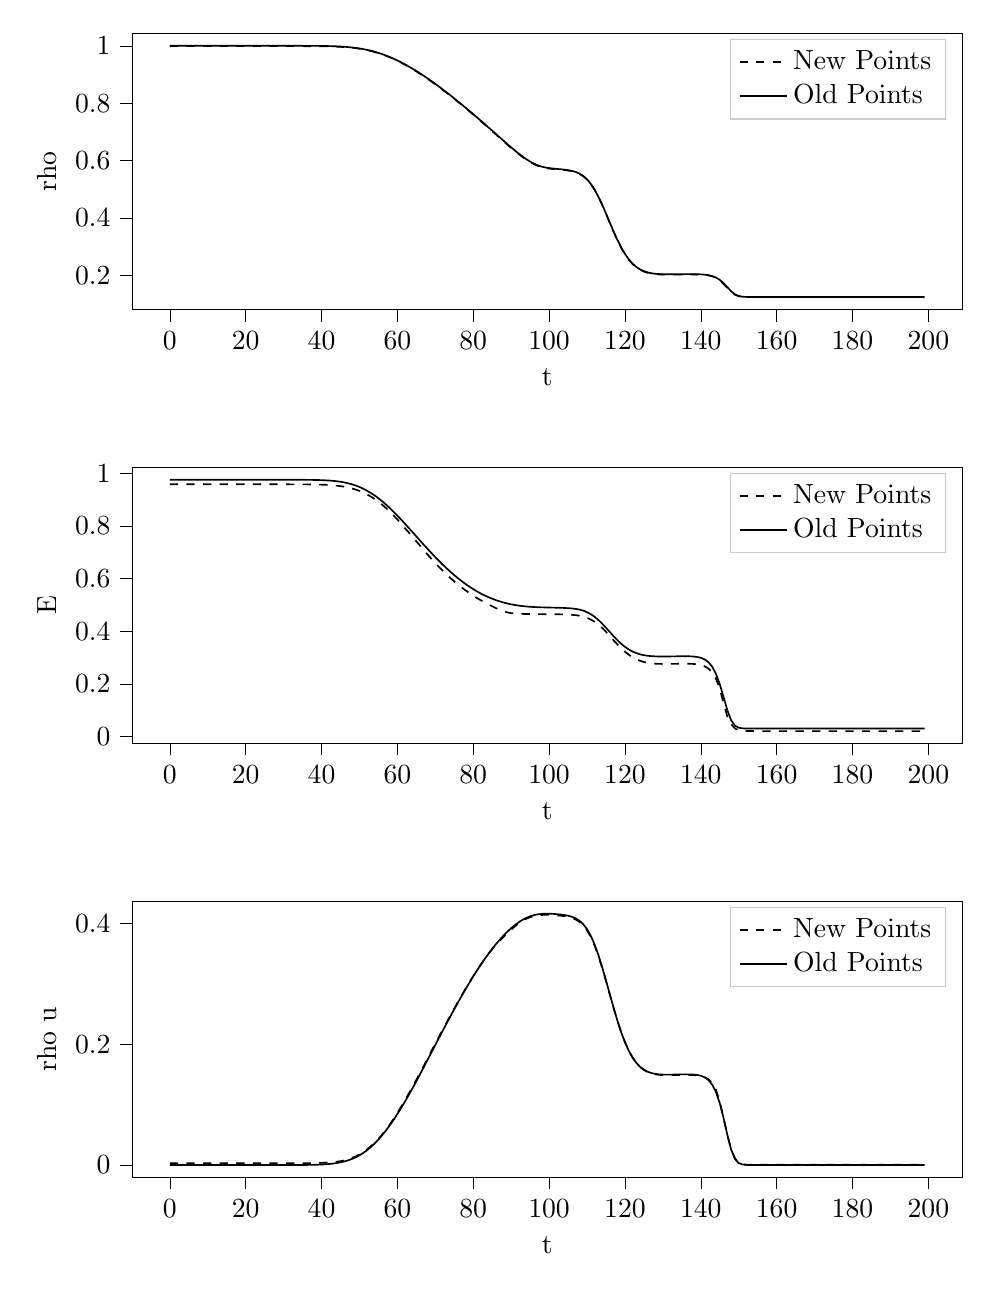
\begin{tikzpicture}

\begin{groupplot}[group style={group size=1 by 3, horizontal sep=2cm, vertical sep=2cm}]
\nextgroupplot[
legend cell align={left},
legend style={fill opacity=0.8, draw opacity=1, text opacity=1, draw=white!80!black},
tick align=outside,
tick pos=left,
x grid style={white!69.0196078431373!black},
xlabel={t},
xmin=-9.95, xmax=208.95,
xtick style={color=black},
y grid style={white!69.0196078431373!black},
ylabel={rho},
ymin=0.080687323773893, ymax=1.04377678433518,
ytick style={color=black},
width=\textwidth,
height=.42\textwidth
]
\addplot [semithick, black, dashed]
table {%
0 0.99882524169784
1 0.99882524169784
2 0.99882524169784
3 0.99882524169784
4 0.99882524169784
5 0.99882524169784
6 0.99882524169784
7 0.99882524169784
8 0.99882524169784
9 0.99882524169784
10 0.99882524169784
11 0.99882524169784
12 0.99882524169784
13 0.99882524169784
14 0.99882524169784
15 0.99882524169784
16 0.99882524169784
17 0.99882524169784
18 0.99882524169784
19 0.998825285764607
20 0.998825281850049
21 0.998825287196158
22 0.998825343014005
23 0.998825180089514
24 0.998825028643488
25 0.998825032144897
26 0.998824636647045
27 0.998824237777124
28 0.998823365635982
29 0.998822033533636
30 0.998819838949506
31 0.998816271919681
32 0.998810721186035
33 0.998801711809176
34 0.998787917137079
35 0.998766632759206
36 0.998734505214823
37 0.998686725283412
38 0.99861710598679
39 0.998517132137085
40 0.998375721291332
41 0.998178669263162
42 0.997909361874113
43 0.997546766712695
44 0.997066969632203
45 0.996442082984878
46 0.995638641183183
47 0.994608519130108
48 0.993330374885918
49 0.991767805468679
50 0.98988582305517
51 0.987650704272657
52 0.98503197259377
53 0.982002546490712
54 0.978540018436696
55 0.974627037067024
56 0.970251305516577
57 0.965405998768861
58 0.96008917738822
59 0.954307466447123
60 0.948065915967038
61 0.941373473624174
62 0.934265596848135
63 0.926855164979088
64 0.91906192600271
65 0.910909834518754
66 0.90242678970644
67 0.893631622380571
68 0.884547266038523
69 0.875196363202017
70 0.865600595413863
71 0.855918955095697
72 0.846033947573116
73 0.83594597328218
74 0.82566982635492
75 0.815217786146208
76 0.804600818180286
77 0.793827454059773
78 0.782905035065573
79 0.771838845237373
80 0.760633212400931
81 0.749329156041814
82 0.737901736440854
83 0.726338323071944
84 0.71465245370466
85 0.702861761492153
86 0.690989382855593
87 0.679133496893696
88 0.667294152315849
89 0.655518341061627
90 0.64417996286244
91 0.633219540959544
92 0.622620158366917
93 0.61257941926789
94 0.603274883496852
95 0.594942451820642
96 0.587810090881552
97 0.582041689878726
98 0.57767220444825
99 0.574542067394456
100 0.572433213741393
101 0.570951743498788
102 0.5697648213078
103 0.568619135985314
104 0.567293201480098
105 0.56554786948231
106 0.563058712250728
107 0.559362096529675
108 0.55383333495392
109 0.545716462966084
110 0.534216805148949
111 0.518654492185445
112 0.498649576108083
113 0.474289370799385
114 0.446215674816509
115 0.41556812190306
116 0.383493884145718
117 0.352005743156572
118 0.322713154696722
119 0.296411442550379
120 0.273734204369341
121 0.254919530798827
122 0.239947071871332
123 0.228371200552992
124 0.219732718745105
125 0.213517525541344
126 0.209217600181896
127 0.206370942005611
128 0.204584163341515
129 0.203539302881556
130 0.202992153655288
131 0.202763449224455
132 0.20272701766468
133 0.202797426145713
134 0.202918252042974
135 0.203051163051173
136 0.203166843817972
137 0.203235733330915
138 0.203218495969337
139 0.203052010680179
140 0.202629264584595
141 0.201764090922016
142 0.200131807315558
143 0.197279501070602
144 0.192334475646371
145 0.183846336147512
146 0.170593505628672
147 0.155764461994924
148 0.143352696739804
149 0.133293523333811
150 0.127622054817377
151 0.125407567204722
152 0.124723707745966
153 0.124533386047822
154 0.124482423111367
155 0.124468920626453
156 0.124465403723982
157 0.124464423907208
158 0.124464194210969
159 0.124464142337939
160 0.124464136520787
161 0.124464140322912
162 0.12446411743577
163 0.12446411743577
164 0.12446411743577
165 0.12446411743577
166 0.12446411743577
167 0.12446411743577
168 0.12446411743577
169 0.12446411743577
170 0.12446411743577
171 0.12446411743577
172 0.12446411743577
173 0.12446411743577
174 0.12446411743577
175 0.12446411743577
176 0.12446411743577
177 0.12446411743577
178 0.12446411743577
179 0.12446411743577
180 0.12446411743577
181 0.12446411743577
182 0.12446411743577
183 0.12446411743577
184 0.12446411743577
185 0.12446411743577
186 0.12446411743577
187 0.12446411743577
188 0.12446411743577
189 0.12446411743577
190 0.12446411743577
191 0.12446411743577
192 0.12446411743577
193 0.12446411743577
194 0.12446411743577
195 0.12446411743577
196 0.12446411743577
197 0.12446411743577
198 0.12446411743577
199 0.12446411743577
};
\addlegendentry{New Points}
\addplot [semithick, black]
table {%
0 0.999999990673304
1 0.999999990673304
2 0.999999990673304
3 0.999999990673304
4 0.999999990673304
5 0.999999990673304
6 0.999999990673304
7 0.999999990673304
8 0.999999990673304
9 0.999999990673304
10 0.999999990673304
11 0.999999990673304
12 0.999999990673304
13 0.999999990673304
14 0.999999990673304
15 0.999999990673188
16 0.999999990613363
17 0.99999998959752
18 0.999999989341796
19 0.999999984189477
20 0.999999973705739
21 0.999999951425917
22 0.99999995951019
23 0.999999900219864
24 0.99999980007917
25 0.99999963899472
26 0.999999344600917
27 0.99999886382409
28 0.999998048154685
29 0.999996655394727
30 0.999994388636926
31 0.999990666875463
32 0.999984733015574
33 0.99997537196386
34 0.999960809257829
35 0.999938501687345
36 0.999904842251513
37 0.999854870748117
38 0.999781888291585
39 0.999676849687996
40 0.99952827617622
41 0.999321538908886
42 0.999038555556407
43 0.998657700894059
44 0.998153564128933
45 0.997497287289296
46 0.996657007765684
47 0.995598465740345
48 0.994286256311325
49 0.992684725953645
50 0.990759336531942
51 0.988478056666465
52 0.985812342425932
53 0.982738189670356
54 0.979236729911257
55 0.975294755102387
56 0.970904559180468
57 0.966063958937712
58 0.960775714159816
59 0.955047109745011
60 0.948889019250931
61 0.942315480216448
62 0.935342680914344
63 0.927988589260379
64 0.920272104023719
65 0.912212625070337
66 0.903829678553893
67 0.895142440701454
68 0.886169650813236
69 0.876929267310902
70 0.867438446443597
71 0.857713326750228
72 0.84776922541252
73 0.837620442322955
74 0.827280454312959
75 0.816761863636921
76 0.806076603030751
77 0.795236088048208
78 0.784251224307334
79 0.773132816128772
80 0.761891760500021
81 0.750539352596095
82 0.739087758838422
83 0.727550672809244
84 0.71594404972236
85 0.704287170689175
86 0.692604208052038
87 0.680926168455306
88 0.669293753880677
89 0.657760944896155
90 0.646399950130127
91 0.635307293347168
92 0.624610221787421
93 0.614472535538927
94 0.605095016449397
95 0.596704246916693
96 0.589521621766072
97 0.583707964721958
98 0.579297606549855
99 0.576156310627358
100 0.574000969870334
101 0.57248017291299
102 0.571264193067916
103 0.570086381495837
104 0.568721459631689
105 0.566925172589584
106 0.564365800656326
107 0.560570524896373
108 0.554906072422308
109 0.546613496220884
110 0.534908962541823
111 0.519142269323688
112 0.498978610612388
113 0.474548688260012
114 0.44651214810282
115 0.41600336139232
116 0.38446686258085
117 0.35342828868708
118 0.324264598637066
119 0.29803157039005
120 0.275379775385168
121 0.25655829879967
122 0.24148162128753
123 0.229826474611315
124 0.221130573302213
125 0.214876147283397
126 0.2105516372068
127 0.207691965234525
128 0.205900478192891
129 0.204856777255547
130 0.204314511505395
131 0.204092814859263
132 0.204064484102008
133 0.204143253944278
134 0.204271664259139
135 0.204410154381753
136 0.204527211631632
137 0.204589750987957
138 0.204552165688165
139 0.204341779785345
140 0.203837538442359
141 0.202838126291723
142 0.201017081225308
143 0.197870636883496
144 0.192691646792645
145 0.184667359904606
146 0.173289805197553
147 0.159203833119233
148 0.144954932228184
149 0.134090938302014
150 0.128237749005468
151 0.125970042293352
152 0.125265819953518
153 0.125069120676745
154 0.125016332797805
155 0.125002354203519
156 0.124998671078932
157 0.12499770244925
158 0.124997447162466
159 0.124997380777701
160 0.124997368455257
161 0.124997359647132
162 0.124997358303174
163 0.124997358176193
164 0.12499735816873
165 0.12499735816873
166 0.12499735816873
167 0.12499735816873
168 0.12499735816873
169 0.12499735816873
170 0.12499735816873
171 0.12499735816873
172 0.12499735816873
173 0.12499735816873
174 0.12499735816873
175 0.12499735816873
176 0.12499735816873
177 0.12499735816873
178 0.12499735816873
179 0.12499735816873
180 0.12499735816873
181 0.12499735816873
182 0.12499735816873
183 0.12499735816873
184 0.12499735816873
185 0.12499735816873
186 0.12499735816873
187 0.12499735816873
188 0.12499735816873
189 0.12499735816873
190 0.12499735816873
191 0.12499735816873
192 0.12499735816873
193 0.12499735816873
194 0.12499735816873
195 0.12499735816873
196 0.12499735816873
197 0.12499735816873
198 0.12499735816873
199 0.12499735816873
};
\addlegendentry{Old Points}

\nextgroupplot[
legend cell align={left},
legend style={fill opacity=0.8, draw opacity=1, text opacity=1, draw=white!80!black},
tick align=outside,
tick pos=left,
x grid style={white!69.0196078431373!black},
xlabel={t},
xmin=-9.95, xmax=208.95,
xtick style={color=black},
y grid style={white!69.0196078431373!black},
ylabel={E},
ymin=-0.0268046259138383, ymax=1.02270497699313,
ytick style={color=black},
width=\textwidth,
height=.42\textwidth
]
\addplot [semithick, black, dashed]
table {%
0 0.957672578985963
1 0.957672578985963
2 0.957672578985963
3 0.957672578985963
4 0.957672578985963
5 0.957672578985963
6 0.957672578985963
7 0.957672578985963
8 0.957672578985963
9 0.957672578985963
10 0.957672578985963
11 0.957672578985963
12 0.957672578985963
13 0.957672578985963
14 0.957672578985963
15 0.957672578985963
16 0.957672578985963
17 0.957672578985963
18 0.957672578985963
19 0.957672753173849
20 0.957672904795495
21 0.957672903052621
22 0.957673035720186
23 0.95767251607196
24 0.957672109987853
25 0.957672123903651
26 0.95767115287741
27 0.957669648914574
28 0.957667379526092
29 0.957663558145871
30 0.957657192044156
31 0.9576469807895
32 0.957630576533468
33 0.957604963192946
34 0.957565092479773
35 0.957503232829951
36 0.957410769693711
37 0.957273486836761
38 0.957072767029239
39 0.956785182075982
40 0.956378868749246
41 0.955814157486872
42 0.95504244525582
43 0.954005560236759
44 0.952635672947182
45 0.950855125041976
46 0.948578561408243
47 0.945704492631743
48 0.942151508268423
49 0.937827174422019
50 0.932645222395822
51 0.926526741579703
52 0.919406152580419
53 0.911231262448939
54 0.901967814966234
55 0.8915999773523
56 0.880130307887591
57 0.86758075277333
58 0.853989816110631
59 0.83958899967828
60 0.824313139688862
61 0.808125573033719
62 0.791324866073787
63 0.775033071942744
64 0.758255749690644
65 0.741225534266522
66 0.724333108836269
67 0.707447180080594
68 0.690679664390643
69 0.674137705867198
70 0.657921207384453
71 0.643196746462645
72 0.628987863705936
73 0.6152381762173
74 0.602002008463447
75 0.589321839438225
76 0.577228728112935
77 0.565740532063752
78 0.554863188282123
79 0.5445882529047
80 0.534894224069938
81 0.525942286362573
82 0.517539315100405
83 0.509540992725169
84 0.501920822445923
85 0.494649583910605
86 0.487697111419727
87 0.481760523098042
88 0.476354612044293
89 0.471345077861615
90 0.468706262593092
91 0.467414611596512
92 0.466425847375955
93 0.465778759738145
94 0.465334247842185
95 0.465055793725675
96 0.464900320624212
97 0.46482051855291
98 0.464770352711943
99 0.464678119483416
100 0.46461441803351
101 0.464503145252806
102 0.464324612685315
103 0.464072718391492
104 0.463707654632884
105 0.463155560490354
106 0.46229158694566
107 0.460923435877268
108 0.458782925905255
109 0.455538505069044
110 0.45083108033571
111 0.444334102407281
112 0.435817252915969
113 0.425196545097015
114 0.412552028408525
115 0.398091998936806
116 0.381586886046344
117 0.365306083097971
118 0.350394601584548
119 0.335980664761936
120 0.322637359183457
121 0.31086619506323
122 0.301364388264135
123 0.293633137664058
124 0.287635641223162
125 0.283204614009741
126 0.280095681376509
127 0.278039570128984
128 0.276779889772552
129 0.276093844877802
130 0.27580236036156
131 0.275769132757182
132 0.275892834320999
133 0.276099135029914
134 0.276328056523863
135 0.276520435234836
136 0.276600844549956
137 0.276453789210773
138 0.275887720984523
139 0.274574835825998
140 0.271956567719277
141 0.267084932961406
142 0.258378685759482
143 0.243851642653307
144 0.219989984390418
145 0.181521509834529
146 0.126840940575295
147 0.0762815965064556
148 0.0472970221029818
149 0.0307330087251987
150 0.0239551859394852
151 0.0217567824407398
152 0.0211307088912848
153 0.0209614275061188
154 0.0209164620400957
155 0.0209046279203357
156 0.0209015104480952
157 0.0209006531989645
158 0.0209004104250447
159 0.020900376016419
160 0.0209003609216696
161 0.0209003817800258
162 0.0209003560364786
163 0.0209003560364786
164 0.0209003560364786
165 0.0209003560364786
166 0.0209003560364786
167 0.0209003560364786
168 0.0209003560364786
169 0.0209003560364786
170 0.0209003560364786
171 0.0209003560364786
172 0.0209003560364786
173 0.0209003560364786
174 0.0209003560364786
175 0.0209003560364786
176 0.0209003560364786
177 0.0209003560364786
178 0.0209003560364786
179 0.0209003560364786
180 0.0209003560364786
181 0.0209003560364786
182 0.0209003560364786
183 0.0209003560364786
184 0.0209003560364786
185 0.0209003560364786
186 0.0209003560364786
187 0.0209003560364786
188 0.0209003560364786
189 0.0209003560364786
190 0.0209003560364786
191 0.0209003560364786
192 0.0209003560364786
193 0.0209003560364786
194 0.0209003560364786
195 0.0209003560364786
196 0.0209003560364786
197 0.0209003560364786
198 0.0209003560364786
199 0.0209003560364786
};
\addlegendentry{New Points}
\addplot [semithick, black]
table {%
0 0.974999995042816
1 0.974999995042816
2 0.974999995042816
3 0.974999995042816
4 0.974999995042816
5 0.974999995042816
6 0.974999995042816
7 0.974999995042816
8 0.974999995042816
9 0.974999995042816
10 0.974999995042816
11 0.974999995042816
12 0.974999995042816
13 0.974999995042815
14 0.974999995042815
15 0.974999995040117
16 0.974999994390443
17 0.974999988766483
18 0.97499998666126
19 0.974999966278458
20 0.974999936063711
21 0.974999894245644
22 0.974999821242071
23 0.974999652773641
24 0.974999345359749
25 0.974998846983031
26 0.97499793789597
27 0.974996422178415
28 0.974993819595234
29 0.974989494425743
30 0.97498236455561
31 0.974970794691552
32 0.974952298603336
33 0.974923154922117
34 0.974877916922401
35 0.974808724309834
36 0.974704596519527
37 0.974550306175209
38 0.974325360954196
39 0.974002626110439
40 0.973547309928343
41 0.97291559377799
42 0.972053851183031
43 0.97089837513597
44 0.969375495221348
45 0.967402862245016
46 0.964891444005473
47 0.961748599386942
48 0.957881996826705
49 0.953203950552913
50 0.947636173616785
51 0.941114245414308
52 0.933591574727766
53 0.925042160923921
54 0.915462469745621
55 0.904871851688637
56 0.893311577600627
57 0.880843056888218
58 0.867545057974408
59 0.853510370151345
60 0.838842194111669
61 0.823650686069139
62 0.808049447188074
63 0.792152686027024
64 0.776072554891447
65 0.759917029162809
66 0.743788383907755
67 0.727781996883469
68 0.711985524234487
69 0.696478519535467
70 0.681332190139397
71 0.666609447942655
72 0.652365100953817
73 0.638646216208521
74 0.625492417779656
75 0.612936319156326
76 0.601004088743318
77 0.589715779116801
78 0.579085824636705
79 0.56912345842663
80 0.559833189972154
81 0.551215060251501
82 0.543265030402672
83 0.53597533714174
84 0.529334635552516
85 0.523328331367785
86 0.517938657828029
87 0.513144832173018
88 0.508923150384679
89 0.50524677890721
90 0.502085847119693
91 0.499407146515095
92 0.49717384750643
93 0.495345327448748
94 0.493877113332056
95 0.492721320202923
96 0.491828000501157
97 0.491146767161147
98 0.49062845457999
99 0.490225564814269
100 0.48989204847478
101 0.489583251578356
102 0.489255653991308
103 0.48886247609099
104 0.488342208518255
105 0.48759974297161
106 0.486483398480378
107 0.484763993686122
108 0.482126550495293
109 0.478186640054635
110 0.472539385217378
111 0.464838894824657
112 0.454891320014267
113 0.442734169403476
114 0.428673267402038
115 0.413260860814231
116 0.397217275928644
117 0.381317979640253
118 0.366277586985864
119 0.352659680800323
120 0.340828994655033
121 0.330947002823028
122 0.323000349900211
123 0.31684647119201
124 0.312262768380073
125 0.308989981719108
126 0.306765700697848
127 0.305347188452543
128 0.304524632255291
129 0.304126409286706
130 0.30401862388768
131 0.304100449984317
132 0.304296837463355
133 0.30454936468815
134 0.30480537794366
135 0.305004373515265
136 0.305059433770516
137 0.304829612508351
138 0.304076596868815
139 0.302395777320979
140 0.299109140283267
141 0.293110237169807
142 0.282676384964858
143 0.265350694817802
144 0.238216455582864
145 0.199238533073085
146 0.150286651411289
147 0.100222395865669
148 0.0619544981807095
149 0.041488457103417
150 0.0337211702159827
151 0.0313715717347596
152 0.0307261912823063
153 0.030554080629536
154 0.030508565921638
155 0.0304965655942388
156 0.030493406901334
157 0.0304925766546751
158 0.0304923586543065
159 0.0304923019172621
160 0.0304922874403655
161 0.0304922829754706
162 0.0304922817529242
163 0.0304922815375214
164 0.0304922815140779
165 0.0304922815140744
166 0.0304922815140744
167 0.0304922815140744
168 0.0304922815140744
169 0.0304922815140744
170 0.0304922815140744
171 0.0304922815140744
172 0.0304922815140744
173 0.0304922815140744
174 0.0304922815140744
175 0.0304922815140744
176 0.0304922815140744
177 0.0304922815140744
178 0.0304922815140744
179 0.0304922815140744
180 0.0304922815140744
181 0.0304922815140744
182 0.0304922815140744
183 0.0304922815140744
184 0.0304922815140744
185 0.0304922815140744
186 0.0304922815140744
187 0.0304922815140744
188 0.0304922815140744
189 0.0304922815140744
190 0.0304922815140744
191 0.0304922815140744
192 0.0304922815140744
193 0.0304922815140744
194 0.0304922815140744
195 0.0304922815140744
196 0.0304922815140744
197 0.0304922815140744
198 0.0304922815140744
199 0.0304922815140744
};
\addlegendentry{Old Points}

\nextgroupplot[
legend cell align={left},
legend style={fill opacity=0.8, draw opacity=1, text opacity=1, draw=white!80!black},
tick align=outside,
tick pos=left,
x grid style={white!69.0196078431373!black},
xlabel={t},
xmin=-9.95, xmax=208.95,
xtick style={color=black},
y grid style={white!69.0196078431373!black},
ylabel={rho u},
ymin=-0.0207805762608243, ymax=0.43639210147731,
ytick style={color=black},
width=\textwidth,
height=.42\textwidth
]
\addplot [semithick, black, dashed]
table {%
0 0.00290458884785963
1 0.00290458884785963
2 0.00290458884785963
3 0.00290458884785963
4 0.00290458884785963
5 0.00290458884785963
6 0.00290458884785963
7 0.00290458884785963
8 0.00290458884785963
9 0.00290458884785963
10 0.00290458884785963
11 0.00290458884785963
12 0.00290458884785963
13 0.00290458884785963
14 0.00290458884785963
15 0.00290458884785963
16 0.00290458884785963
17 0.00290458884785963
18 0.00290458884785963
19 0.00290458394564734
20 0.0029045798609936
21 0.00290453752212418
22 0.00290475929793749
23 0.00290465229195426
24 0.00290469227330546
25 0.00290486393320261
26 0.00290548578456837
27 0.00290602204269107
28 0.00290708676152179
29 0.00290915015229539
30 0.0029124045051012
31 0.00291745563300709
32 0.00292580134352904
33 0.00293883050035891
34 0.00295902036016327
35 0.00299017722534492
36 0.00303712247772692
37 0.00310677646369859
38 0.00320819717566446
39 0.00335434241533328
40 0.00356079782854247
41 0.00384770149876194
42 0.00423999749053753
43 0.00476740527663387
44 0.00546482035026193
45 0.00637090306284628
46 0.00758525506482067
47 0.00938696534848443
48 0.0116155597173434
49 0.0143284232912522
50 0.0175801197424472
51 0.0214201062160434
52 0.0258904800911598
53 0.0310234367959282
54 0.0368416750661412
55 0.0433571772364309
56 0.0505692701598554
57 0.0584680701771409
58 0.0670334190276578
59 0.0762592365302957
60 0.0860905153685961
61 0.0964677359016576
62 0.107270845274374
63 0.118126649452192
64 0.129311408828176
65 0.140784386407259
66 0.152527308365973
67 0.164450431565947
68 0.1765009065808
69 0.188627862849587
70 0.200782869387291
71 0.212528973327071
72 0.224208922839458
73 0.235827293635022
74 0.247347752091503
75 0.258735181647768
76 0.269954605115903
77 0.280971448814856
78 0.291750674174669
79 0.302256354475315
80 0.312451374949641
81 0.322210431062409
82 0.331557854808674
83 0.340491301642779
84 0.34895081092825
85 0.356876727202102
86 0.364210222988701
87 0.371119973141863
88 0.377415281058704
89 0.383019998253524
90 0.389005501758852
91 0.394800720016572
92 0.399804469064216
93 0.403946128813236
94 0.407281968882151
95 0.40983647593845
96 0.411664927114986
97 0.41285253480266
98 0.413508011366744
99 0.41372375754337
100 0.413681120268987
101 0.413418156911564
102 0.412975641855892
103 0.412365587724015
104 0.411536506867285
105 0.4103691383466
106 0.408653625770651
107 0.406065937478925
108 0.40215935483953
109 0.396391170221175
110 0.388196097333467
111 0.377104562932817
112 0.362879600044014
113 0.345629059708916
114 0.325845305405085
115 0.304334315892937
116 0.281822107946037
117 0.259898702669057
118 0.239092878285504
119 0.220157936351893
120 0.203573407876687
121 0.189561506425067
122 0.177963614365081
123 0.168893037764296
124 0.162057949409467
125 0.157103123601485
126 0.153657925110422
127 0.15137347411375
128 0.149944775886111
129 0.149120855084825
130 0.14870634437248
131 0.14855599689867
132 0.148565978787194
133 0.148663991851022
134 0.148799134477198
135 0.148931332789299
136 0.149021219032903
137 0.149017696893704
138 0.148841775923059
139 0.148361104729965
140 0.147349680117499
141 0.145421115741961
142 0.141918545474813
143 0.135492132663692
144 0.124223380536106
145 0.10572224541142
146 0.0783318423386507
147 0.0491504412031782
148 0.0268933306089233
149 0.011254642474681
150 0.00388637640309602
151 0.00134874155765786
152 0.000614489180180337
153 0.000415296572752264
154 0.000362343864279199
155 0.000348369799783428
156 0.000344683703721135
157 0.000343697708062461
158 0.000343457215172603
159 0.00034337611957822
160 0.000343381848946375
161 0.000343396624415818
162 0.000343377814005421
163 0.000343377814005421
164 0.000343377814005421
165 0.000343377814005421
166 0.000343377814005421
167 0.000343377814005421
168 0.000343377814005421
169 0.000343377814005421
170 0.000343377814005421
171 0.000343377814005421
172 0.000343377814005421
173 0.000343377814005421
174 0.000343377814005421
175 0.000343377814005421
176 0.000343377814005421
177 0.000343377814005421
178 0.000343377814005421
179 0.000343377814005421
180 0.000343377814005421
181 0.000343377814005421
182 0.000343377814005421
183 0.000343377814005421
184 0.000343377814005421
185 0.000343377814005421
186 0.000343377814005421
187 0.000343377814005421
188 0.000343377814005421
189 0.000343377814005421
190 0.000343377814005421
191 0.000343377814005421
192 0.000343377814005421
193 0.000343377814005421
194 0.000343377814005421
195 0.000343377814005421
196 0.000343377814005421
197 0.000343377814005421
198 0.000343377814005421
199 0.000343377814005421
};
\addlegendentry{New Points}
\addplot [semithick, black]
table {%
0 -2.9701575942379e-17
1 -2.9701575942379e-17
2 -2.9701575942379e-17
3 -2.9701575942379e-17
4 -2.9701575942379e-17
5 -2.9701575942379e-17
6 -2.9701575942379e-17
7 -2.9701575942379e-17
8 -2.9701575942379e-17
9 -2.9701575942379e-17
10 -2.9701575942379e-17
11 -2.9701575942379e-17
12 -2.9701575942379e-17
13 -3.58603575113451e-17
14 -3.58638102426239e-17
15 5.6805661435368e-13
16 1.99042476361002e-10
17 2.20837991649488e-09
18 2.93997368028267e-09
19 1.31357376888643e-08
20 2.38145813217986e-08
21 4.87195462126188e-08
22 1.18482312201542e-07
23 2.0095587206295e-07
24 3.83396059768099e-07
25 6.58121348779825e-07
26 1.16128545818365e-06
27 2.03225357455255e-06
28 3.48646389712185e-06
29 5.97480063111906e-06
30 1.00168031352998e-05
31 1.66154888208619e-05
32 2.71792475439631e-05
33 4.38360783100733e-05
34 6.9738147530809e-05
35 0.000109360034940665
36 0.000169110916869244
37 0.000257759063581096
38 0.000387167364876908
39 0.000573117748608961
40 0.000835869786797033
41 0.00120107973443098
42 0.00170018895588471
43 0.00237086844167696
44 0.00325687357947661
45 0.00440760492585291
46 0.0058770045036118
47 0.00772213506918395
48 0.0100010852238978
49 0.0127705763429908
50 0.0160835079558624
51 0.0199864997521351
52 0.0245176736126449
53 0.029704885273648
54 0.0355645653482579
55 0.0421012893858932
56 0.0493077793042677
57 0.0571655985840627
58 0.0656463751672976
59 0.07471303783688
60 0.0843216061489801
61 0.0944227378619742
62 0.104963347960292
63 0.115888113820293
64 0.127140629164304
65 0.138664664012591
66 0.150404853532333
67 0.162307518067251
68 0.174321041457807
69 0.186396266022466
70 0.198486618269269
71 0.210548312786717
72 0.222540185550889
73 0.234423749038626
74 0.24616309786956
75 0.257724580624995
76 0.269076805027718
77 0.280190349490242
78 0.291037541508123
79 0.301592220966071
80 0.311829593524858
81 0.321725891157009
82 0.331258108006691
83 0.34040380705866
84 0.349140751931193
85 0.357446640915221
86 0.365298701484088
87 0.372673393425291
88 0.379546061984702
89 0.3858904907899
90 0.391678889356953
91 0.396881980119472
92 0.401469837523235
93 0.405414023679009
94 0.408691643888321
95 0.411292021579195
96 0.413226034663786
97 0.41453519470013
98 0.415295784669826
99 0.415611525216486
100 0.415593772491148
101 0.415336270698027
102 0.41489544485938
103 0.414279735123743
104 0.413441921116945
105 0.412265562656191
106 0.41054307470679
107 0.407952698513731
108 0.404050230313847
109 0.398294142046233
110 0.390116252725716
111 0.379034700041386
112 0.364785466199088
113 0.347433290718267
114 0.327421677785053
115 0.305538970309093
116 0.282804902037727
117 0.260309643297353
118 0.239050560230286
119 0.219807538955069
120 0.20307934623608
121 0.189081108725716
122 0.17778662249403
123 0.168993003883264
124 0.162388542113512
125 0.157611733837737
126 0.154296588877
127 0.152103708794801
128 0.150738703044433
129 0.149960169583879
130 0.149579864110399
131 0.149457424423213
132 0.149491946494713
133 0.149612014228558
134 0.149765301786734
135 0.149907796060004
136 0.149991959449217
137 0.149952034921847
138 0.149683391104505
139 0.149011228633714
140 0.147642222218352
141 0.145092235684392
142 0.140589882050874
143 0.132983875095863
144 0.120763964502009
145 0.10247138701595
146 0.0779153039253849
147 0.0500927752607743
148 0.0255869634889079
149 0.010102976420237
150 0.00323067095348623
151 0.000916686735148521
152 0.000247536233262668
153 6.57017337512221e-05
154 1.73342190031844e-05
155 4.56262885444554e-06
156 1.19902286403957e-06
157 3.14993485349219e-07
158 8.20702035475298e-08
159 2.12618186030591e-08
160 5.83523126442528e-09
161 1.06852817499928e-09
162 1.53347718367724e-10
163 1.33942684000716e-11
164 1.28520434948373e-15
165 5.28135721761187e-19
166 5.28135721758471e-19
167 5.28135721758267e-19
168 5.2813572175825e-19
169 5.28135721758248e-19
170 5.28135721758248e-19
171 5.28135721758248e-19
172 5.28135721758248e-19
173 5.28135721758248e-19
174 5.28135721758248e-19
175 5.28135721758248e-19
176 5.28135721758248e-19
177 5.28135721758248e-19
178 5.28135721758248e-19
179 5.28135721758248e-19
180 5.28135721758248e-19
181 5.28135721758248e-19
182 5.28135721758248e-19
183 5.28135721758248e-19
184 5.28135721758248e-19
185 5.28135721758248e-19
186 5.28135721758248e-19
187 5.28135721758248e-19
188 5.28135721758248e-19
189 5.28135721758248e-19
190 5.28135721758248e-19
191 5.28135721758248e-19
192 5.28135721758248e-19
193 5.28135721758248e-19
194 5.28135721758248e-19
195 5.28135721758248e-19
196 5.28135721758248e-19
197 5.28135721758248e-19
198 5.28135721758248e-19
199 5.28135721758248e-19
};
\addlegendentry{Old Points}
\end{groupplot}

\end{tikzpicture}

	\caption{Resulting macroscopic quantities $\rho$, E, $\rho$u after interpolating in time using the interpolation method described in \ref{Reduced Order Model}. The interpolated quantity lies at timestamp t=24,5, while the original quantity lies at timestamp t=25.}
\end{figure}
\subsection{Rarefied Regime}
\subsection{Discussion and Outlook}
\newpage
\bibliography{Bibliography}{}
\bibliographystyle{unsrt}
\newpage
\subsection{Appendix A}\label{AppendixA}
\begin{center}
	\begin{figure}[htbp!]
		\scalebox{.9}{% This file was created by tikzplotlib v0.9.6.
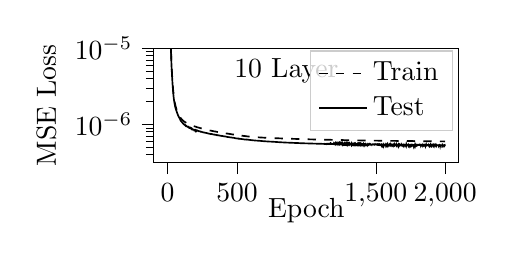
\begin{tikzpicture}

\begin{axis}[
legend cell align={left},
legend style={fill opacity=0.8, draw opacity=1, text opacity=1, draw=white!80!black},
log basis y={10},
tick align=outside,
tick pos=left,
title={10 Layer $\rare$},
title style={at={(0.45,0.85)},anchor=north},
x grid style={white!69.0196078431373!black},
xlabel={Epoch},
x label style={yshift=10pt},
xmin=-99.95, xmax=2098.95,
xtick style={color=black},
xtick = {0,500,1500,2000},
y grid style={white!69.0196078431373!black},
ylabel={MSE Loss},
ymin=3.17093839325154e-07, ymax=1e-5,
ymode=log,
ytick style={color=black},
width=0.45\textwidth,
height=0.25\textwidth
]
\addplot [semithick, black, dashed]
table {%
0 0.00997787586692721
1 0.0027661414751783
2 0.00218623768771067
3 0.00185343958390877
4 0.00115804947796278
5 0.00036777743147104
6 0.00018824286320887
7 0.000164930714039656
8 0.000153345151928079
9 0.000141543177305721
10 0.000127938025187177
11 0.000112482768548944
12 9.57521400996484e-05
13 7.92569487603032e-05
14 6.42920351929206e-05
15 5.20401717658388e-05
16 4.29740166491683e-05
17 3.62663831710961e-05
18 3.07352183917828e-05
19 2.49385155948403e-05
20 2.06156149879462e-05
21 1.71943852956247e-05
22 1.4385688823495e-05
23 1.20649838572717e-05
24 1.02233446727951e-05
25 8.78601411159252e-06
26 7.68138640933103e-06
27 6.83470541434872e-06
28 6.17248770799961e-06
29 5.6463688954409e-06
30 5.22004835283951e-06
31 4.84264568081016e-06
32 4.50758502950066e-06
33 4.20824098557659e-06
34 3.93843728591037e-06
35 3.69604697584691e-06
36 3.4781861807005e-06
37 3.27953066255304e-06
38 3.102444766796e-06
39 2.94624955324707e-06
40 2.80618139169064e-06
41 2.6809971720354e-06
42 2.57034235244191e-06
43 2.47136843603357e-06
44 2.38247599895658e-06
45 2.3052505364376e-06
46 2.2339168820622e-06
47 2.16824932778081e-06
48 2.10921677893339e-06
49 2.05554289499332e-06
50 2.00520992609654e-06
51 1.96032569562021e-06
52 1.91601798240981e-06
53 1.87716817765704e-06
54 1.84075475442569e-06
55 1.8041044749566e-06
56 1.77211888149031e-06
57 1.74144628215345e-06
58 1.71423015325445e-06
59 1.68766705314738e-06
60 1.66201588962167e-06
61 1.63708562206466e-06
62 1.61347263502876e-06
63 1.5917540299597e-06
64 1.57049718154667e-06
65 1.55085114516851e-06
66 1.53163219016506e-06
67 1.51338286417513e-06
68 1.49671406592233e-06
69 1.47951891813136e-06
70 1.4645103722728e-06
71 1.44944799347968e-06
72 1.43420475933453e-06
73 1.41955645852931e-06
74 1.40517172491172e-06
75 1.39141421908562e-06
76 1.37808219858471e-06
77 1.3657449522384e-06
78 1.3527578432786e-06
79 1.34140151624251e-06
80 1.32919058387415e-06
81 1.31819503866382e-06
82 1.30771289047971e-06
83 1.29784039592096e-06
84 1.28814695580104e-06
85 1.27880892563326e-06
86 1.27049044516525e-06
87 1.26170827212491e-06
88 1.25354349086138e-06
89 1.24524294693629e-06
90 1.23696791416705e-06
91 1.22909348488065e-06
92 1.22303059853834e-06
93 1.21662571478964e-06
94 1.20954619882241e-06
95 1.20269462843225e-06
96 1.19554730241589e-06
97 1.18936523608681e-06
98 1.18438249876363e-06
99 1.17871571490014e-06
100 1.17326355984915e-06
101 1.16720301622308e-06
102 1.16031671996097e-06
103 1.15646743591924e-06
104 1.15072228288682e-06
105 1.1456532542411e-06
106 1.14082713997732e-06
107 1.13676369537075e-06
108 1.13183904920788e-06
109 1.12775252654274e-06
110 1.12097592221971e-06
111 1.11884615537861e-06
112 1.11495200479794e-06
113 1.11073350669244e-06
114 1.10769001994981e-06
115 1.10351587494506e-06
116 1.10006028367593e-06
117 1.09647195202456e-06
118 1.09295321027503e-06
119 1.08959795028341e-06
120 1.08633151981508e-06
121 1.08298288154174e-06
122 1.0800084913285e-06
123 1.07806380844977e-06
124 1.074994691038e-06
125 1.07166258550251e-06
126 1.06880648237961e-06
127 1.06578414178671e-06
128 1.06304140217617e-06
129 1.06044994532795e-06
130 1.05643772593567e-06
131 1.0558744672835e-06
132 1.05326026272223e-06
133 1.04935598690759e-06
134 1.04676802968129e-06
135 1.04461839976011e-06
136 1.04219356757085e-06
137 1.03843377786461e-06
138 1.03679534922208e-06
139 1.03479115048799e-06
140 1.03239273369127e-06
141 1.02880143617767e-06
142 1.02687638050725e-06
143 1.02502206539157e-06
144 1.02148192920026e-06
145 1.02024824695945e-06
146 1.01793011802442e-06
147 1.01475467491241e-06
148 1.01393682172102e-06
149 1.01059575447948e-06
150 1.00912902482264e-06
151 1.0062060501923e-06
152 1.00506513257415e-06
153 1.00228589985818e-06
154 1.00133910484601e-06
155 9.99022535552285e-07
156 9.96578049466734e-07
157 9.95774760042423e-07
158 9.92670811598373e-07
159 9.90552980908888e-07
160 9.90131076179068e-07
161 9.8754623903119e-07
162 9.8556907477132e-07
163 9.85354359244184e-07
164 9.82352091568828e-07
165 9.80439722610527e-07
166 9.78883942138964e-07
167 9.78459102157103e-07
168 9.75541983876837e-07
169 9.74201690695509e-07
170 9.73315617585513e-07
171 9.7158668955899e-07
172 9.71484288783131e-07
173 9.67737080088682e-07
174 9.66393180931391e-07
175 9.64838651981381e-07
176 9.64215281697989e-07
177 9.62576921267555e-07
178 9.63217306946262e-07
179 9.60148133856364e-07
180 9.59013245392271e-07
181 9.56711457007486e-07
182 9.55200339518569e-07
183 9.53850673880652e-07
184 9.52729099026328e-07
185 9.51356085352018e-07
186 9.49982874573152e-07
187 9.48758935265914e-07
188 9.4734960742926e-07
189 9.46268320717536e-07
190 9.45888197207978e-07
191 9.43202051558956e-07
192 9.42285718593894e-07
193 9.4148136670924e-07
194 9.39797778954699e-07
195 9.38851433886612e-07
196 9.36940359082428e-07
197 9.35960853297502e-07
198 9.35100780367293e-07
199 9.33036782470253e-07
200 9.32759092336255e-07
201 9.309670438995e-07
202 9.30231287497918e-07
203 9.28388456145512e-07
204 9.28534422172334e-07
205 9.26417262860468e-07
206 9.25963449361689e-07
207 9.23892555078964e-07
208 9.23097257839345e-07
209 9.21156167748904e-07
210 9.20179683930655e-07
211 9.18629479031097e-07
212 9.17580147955732e-07
213 9.16587913565081e-07
214 9.15249802602602e-07
215 9.14260038939574e-07
216 9.13397146405259e-07
217 9.12211345678315e-07
218 9.10792389674953e-07
219 9.10044973522872e-07
220 9.09023786704211e-07
221 9.08015798756878e-07
222 9.07080938276295e-07
223 9.05977511166611e-07
224 9.05009585721928e-07
225 9.03722100105142e-07
226 9.0283103281763e-07
227 9.01766764314971e-07
228 9.00620563015764e-07
229 8.99610003187945e-07
230 8.98586724986217e-07
231 8.97490580570093e-07
232 8.96478950949131e-07
233 8.95298846074866e-07
234 8.94353904413947e-07
235 8.93204120927749e-07
236 8.923171830304e-07
237 8.90687736870177e-07
238 8.89868796548399e-07
239 8.88946101269994e-07
240 8.87893214382984e-07
241 8.86297618535537e-07
242 8.85070359657902e-07
243 8.84417957706773e-07
244 8.83675672440631e-07
245 8.8251698130648e-07
246 8.81460606791507e-07
247 8.8027023426207e-07
248 8.79355826469919e-07
249 8.78572113578002e-07
250 8.77525471793206e-07
251 8.76351880549464e-07
252 8.75500791465811e-07
253 8.74678740700574e-07
254 8.73476796158457e-07
255 8.72610606649005e-07
256 8.71706194686794e-07
257 8.70708743093473e-07
258 8.70191305182289e-07
259 8.69344236235747e-07
260 8.67789354629167e-07
261 8.66628777828282e-07
262 8.65958915056808e-07
263 8.64537149453781e-07
264 8.63818404411631e-07
265 8.62849739490912e-07
266 8.61764416811184e-07
267 8.60982841373925e-07
268 8.60051689585362e-07
269 8.59030311005427e-07
270 8.58128868173935e-07
271 8.57145231947243e-07
272 8.56545518360008e-07
273 8.55089079635718e-07
274 8.54582956577588e-07
275 8.53439548222923e-07
276 8.52625509651261e-07
277 8.52064497024685e-07
278 8.50905582069572e-07
279 8.50112307404061e-07
280 8.49598813260855e-07
281 8.4875707469223e-07
282 8.4775906213963e-07
283 8.4675666619205e-07
284 8.46309231747e-07
285 8.45124665829644e-07
286 8.44529056251986e-07
287 8.43495970570984e-07
288 8.42961660282526e-07
289 8.41671420289458e-07
290 8.41705411914972e-07
291 8.40604265988532e-07
292 8.39964006132732e-07
293 8.38750670340005e-07
294 8.3819956410025e-07
295 8.37723511324384e-07
296 8.36425500693849e-07
297 8.35761372655952e-07
298 8.35393352815572e-07
299 8.3392940771887e-07
300 8.3388055014666e-07
301 8.32478889208232e-07
302 8.32139470674065e-07
303 8.31678217167564e-07
304 8.30812586201546e-07
305 8.30091150533008e-07
306 8.29310000142414e-07
307 8.28749091709824e-07
308 8.2756600025391e-07
309 8.27514076803482e-07
310 8.26390768622787e-07
311 8.25961606182091e-07
312 8.25162235912558e-07
313 8.24495962177707e-07
314 8.24095709617723e-07
315 8.22966658319046e-07
316 8.21936873251161e-07
317 8.21767470569057e-07
318 8.20922504203736e-07
319 8.20247862861834e-07
320 8.19370113532614e-07
321 8.18635833951475e-07
322 8.17986851899377e-07
323 8.17315450689193e-07
324 8.1666383891843e-07
325 8.16427804124942e-07
326 8.15375180422961e-07
327 8.15192657825037e-07
328 8.14120937434382e-07
329 8.13174602825484e-07
330 8.1293584187847e-07
331 8.11936721930806e-07
332 8.11085818554602e-07
333 8.10528149429501e-07
334 8.09983656409941e-07
335 8.08851426143065e-07
336 8.08121500682546e-07
337 8.08130491662951e-07
338 8.07360241225297e-07
339 8.06781943225587e-07
340 8.06020081228098e-07
341 8.05330066299348e-07
342 8.04786609791108e-07
343 8.0464047090345e-07
344 8.03382348692594e-07
345 8.03091622429974e-07
346 8.03480803682533e-07
347 8.01579474654091e-07
348 8.0091967774365e-07
349 8.01363648946563e-07
350 7.99436845767332e-07
351 7.99345849031852e-07
352 7.98882536855672e-07
353 7.97898566048616e-07
354 7.98836069549225e-07
355 7.98981313806735e-07
356 7.97069268514861e-07
357 7.96280659386639e-07
358 7.96522883803164e-07
359 7.94783968302681e-07
360 7.94133767442418e-07
361 7.94591968116265e-07
362 7.92818375458637e-07
363 7.92365432204178e-07
364 7.91729609915137e-07
365 7.92124033381469e-07
366 7.9021502497767e-07
367 7.89800760259141e-07
368 7.89006110096579e-07
369 7.89422273101081e-07
370 7.87633119500697e-07
371 7.87470235025012e-07
372 7.86781127885661e-07
373 7.87345359412939e-07
374 7.85442462444053e-07
375 7.85028574483704e-07
376 7.84489331238092e-07
377 7.83982934024152e-07
378 7.84435161477859e-07
379 7.82677077467042e-07
380 7.8204591821418e-07
381 7.81801198940002e-07
382 7.81111819321723e-07
383 7.81425274823278e-07
384 7.7998786557032e-07
385 7.79324741330356e-07
386 7.78943699941692e-07
387 7.78382946805323e-07
388 7.7774481707138e-07
389 7.78080912994028e-07
390 7.76618715718769e-07
391 7.76134723423638e-07
392 7.75627843495386e-07
393 7.74918021193116e-07
394 7.74431415038634e-07
395 7.74660446609232e-07
396 7.73305947575409e-07
397 7.72896880562257e-07
398 7.72197305280997e-07
399 7.71702392796669e-07
400 7.71071945763424e-07
401 7.70523813088175e-07
402 7.70097182538621e-07
403 7.7021479600603e-07
404 7.68894578584423e-07
405 7.68398064082021e-07
406 7.67811163484566e-07
407 7.67315257036216e-07
408 7.66777737169377e-07
409 7.66156092197434e-07
410 7.65690696312049e-07
411 7.65130233787659e-07
412 7.6555170792858e-07
413 7.64065328610286e-07
414 7.63505121966546e-07
415 7.63133862619725e-07
416 7.62454071889351e-07
417 7.62014022313906e-07
418 7.6143167035525e-07
419 7.60892476279196e-07
420 7.60415168230111e-07
421 7.59914973372133e-07
422 7.5941622890241e-07
423 7.60389407474804e-07
424 7.58777384561427e-07
425 7.58338006789927e-07
426 7.57724335500143e-07
427 7.57657803433176e-07
428 7.56923721269232e-07
429 7.56353567965107e-07
430 7.56923098862217e-07
431 7.55219046823186e-07
432 7.54618819826192e-07
433 7.54311231389693e-07
434 7.53780425611694e-07
435 7.54422887609962e-07
436 7.52576872230293e-07
437 7.52243586475743e-07
438 7.51672492100397e-07
439 7.52297821776438e-07
440 7.50493718726375e-07
441 7.50091651326557e-07
442 7.49571382499425e-07
443 7.5027601661759e-07
444 7.48633131451015e-07
445 7.48203038369866e-07
446 7.47641490107753e-07
447 7.4706847775019e-07
448 7.47778209245098e-07
449 7.45882051290891e-07
450 7.45447632596097e-07
451 7.45004974220365e-07
452 7.45590436821431e-07
453 7.44075579518722e-07
454 7.43488029229411e-07
455 7.4302814456928e-07
456 7.43562355694394e-07
457 7.42126745706173e-07
458 7.41440271383453e-07
459 7.41023272865959e-07
460 7.42221455794834e-07
461 7.39916425203546e-07
462 7.39315465096979e-07
463 7.38942567977574e-07
464 7.39466763462815e-07
465 7.38114260798284e-07
466 7.37723011752678e-07
467 7.38328398483645e-07
468 7.36677821834064e-07
469 7.36189456091552e-07
470 7.36971248016971e-07
471 7.35291715386666e-07
472 7.34859717340441e-07
473 7.35544233293695e-07
474 7.33993297529878e-07
475 7.33437984763441e-07
476 7.34147434599208e-07
477 7.32526463366412e-07
478 7.32113129146228e-07
479 7.32783056690778e-07
480 7.31102353171309e-07
481 7.30759978779361e-07
482 7.30174026074337e-07
483 7.3101718700741e-07
484 7.29139022212166e-07
485 7.28747309921118e-07
486 7.29511678514427e-07
487 7.27845423909912e-07
488 7.27509910404933e-07
489 7.27898909303804e-07
490 7.25985288198672e-07
491 7.26988534040629e-07
492 7.26433349939271e-07
493 7.24913795409066e-07
494 7.25639360695141e-07
495 7.25110006783325e-07
496 7.23576190097219e-07
497 7.24332362437963e-07
498 7.23792091548603e-07
499 7.22295086035274e-07
500 7.23148807196594e-07
501 7.22562276394001e-07
502 7.21028598093199e-07
503 7.21920047169533e-07
504 7.20162841702177e-07
505 7.21097849861962e-07
506 7.20601577768321e-07
507 7.18964301626102e-07
508 7.19790344447802e-07
509 7.19423874585345e-07
510 7.17816719657094e-07
511 7.18529795136646e-07
512 7.17035474110617e-07
513 7.17842366498189e-07
514 7.173693042688e-07
515 7.15891436129823e-07
516 7.16593398948362e-07
517 7.16193349916239e-07
518 7.15836237418444e-07
519 7.13896747583931e-07
520 7.14747440071051e-07
521 7.14939811359727e-07
522 7.14682133747146e-07
523 7.14109896080117e-07
524 7.12665502788923e-07
525 7.13412247876022e-07
526 7.12840395792114e-07
527 7.1258078847336e-07
528 7.1094341305411e-07
529 7.11800691419739e-07
530 7.11041270108126e-07
531 7.11053048263466e-07
532 7.09551945874409e-07
533 7.10300355095228e-07
534 7.10044622053374e-07
535 7.08126653066188e-07
536 7.09192354179322e-07
537 7.08688509973854e-07
538 7.08473750933081e-07
539 7.0703383852333e-07
540 7.07924062425036e-07
541 7.07072048214741e-07
542 7.05930014561318e-07
543 7.06833243867777e-07
544 7.06151251620213e-07
545 7.05789116310029e-07
546 7.05411095324848e-07
547 7.03952515351602e-07
548 7.04824918869917e-07
549 7.04396891237025e-07
550 7.04121892809439e-07
551 7.03592790472385e-07
552 7.02295799982267e-07
553 7.03159633289374e-07
554 7.02392406822128e-07
555 7.02389151811644e-07
556 7.02069595888588e-07
557 7.00544815430249e-07
558 7.01544812031329e-07
559 7.01071055104308e-07
560 7.00843794945172e-07
561 7.00298507183561e-07
562 6.99028340818586e-07
563 6.9988211890859e-07
564 6.99153588470836e-07
565 6.99094921657206e-07
566 6.98874052901033e-07
567 6.97493815380312e-07
568 6.9732204678985e-07
569 6.96886004035946e-07
570 6.96496134878544e-07
571 6.96340423658626e-07
572 6.9577226418005e-07
573 6.95301015184668e-07
574 6.94970092226299e-07
575 6.94665715130327e-07
576 6.94327597415167e-07
577 6.9397252194392e-07
578 6.93629053131417e-07
579 6.93304834925357e-07
580 6.92961221275823e-07
581 6.92612403483395e-07
582 6.92295116081709e-07
583 6.92008054087978e-07
584 6.91836038868132e-07
585 6.91154041760456e-07
586 6.91039159349316e-07
587 6.90780433998839e-07
588 6.90375913677599e-07
589 6.90120593674237e-07
590 6.89844487624214e-07
591 6.89540247705622e-07
592 6.8927526524476e-07
593 6.88991556458518e-07
594 6.88708317511555e-07
595 6.88413684557077e-07
596 6.88122735454044e-07
597 6.87847310999246e-07
598 6.87655565940304e-07
599 6.873611031466e-07
600 6.8711852216552e-07
601 6.86813203969905e-07
602 6.86521028598008e-07
603 6.86258257005079e-07
604 6.86011237931439e-07
605 6.85736956057781e-07
606 6.8547543475006e-07
607 6.85227141644873e-07
608 6.84974181766052e-07
609 6.84731802891747e-07
610 6.84444454293498e-07
611 6.84201174820487e-07
612 6.83949088440272e-07
613 6.83735282066777e-07
614 6.83597051065021e-07
615 6.83230357168441e-07
616 6.82977046281508e-07
617 6.82744479377107e-07
618 6.82628084632597e-07
619 6.82269299900895e-07
620 6.82057781943968e-07
621 6.81825706507766e-07
622 6.81707034459578e-07
623 6.81389691763457e-07
624 6.81201359242323e-07
625 6.81054129145764e-07
626 6.8075853309324e-07
627 6.80542225936165e-07
628 6.80400173507678e-07
629 6.80067346735314e-07
630 6.79983958491448e-07
631 6.79618614057631e-07
632 6.79393168169895e-07
633 6.79165578233665e-07
634 6.79077912963066e-07
635 6.78772824926455e-07
636 6.78559704212489e-07
637 6.78351354096662e-07
638 6.78243983884386e-07
639 6.77901727698327e-07
640 6.77708650769659e-07
641 6.77525354845443e-07
642 6.77312835492216e-07
643 6.77094021853009e-07
644 6.7693512350786e-07
645 6.76660766927739e-07
646 6.76465998878939e-07
647 6.7620693066317e-07
648 6.76058081367614e-07
649 6.75807865121669e-07
650 6.75675274962373e-07
651 6.75309103939981e-07
652 6.75240928430298e-07
653 6.75009894337109e-07
654 6.74884714669588e-07
655 6.7469262417319e-07
656 6.74492794075832e-07
657 6.74472121843905e-07
658 6.74072660487468e-07
659 6.74126479594861e-07
660 6.73871772562507e-07
661 6.73676320815275e-07
662 6.73381162670239e-07
663 6.73315533632035e-07
664 6.7304010840985e-07
665 6.7279634778572e-07
666 6.72624413653011e-07
667 6.72622655784494e-07
668 6.72328725286775e-07
669 6.72171628352203e-07
670 6.72120275240218e-07
671 6.72108327890442e-07
672 6.71769079815476e-07
673 6.71592175606861e-07
674 6.7153022288835e-07
675 6.71228376674549e-07
676 6.71063214738865e-07
677 6.70862587298871e-07
678 6.70727474243904e-07
679 6.70538763273498e-07
680 6.70397458648608e-07
681 6.70331136205959e-07
682 6.70071903499547e-07
683 6.69920863757056e-07
684 6.69779470129583e-07
685 6.69620603034105e-07
686 6.69458129848977e-07
687 6.6930754940131e-07
688 6.69167233667167e-07
689 6.68956220224004e-07
690 6.68770538680974e-07
691 6.68667876396967e-07
692 6.68520957177066e-07
693 6.68362044635273e-07
694 6.68231087544768e-07
695 6.68063874257996e-07
696 6.67905007389891e-07
697 6.67740694836993e-07
698 6.67615698802138e-07
699 6.67491615800486e-07
700 6.67331059744924e-07
701 6.67199185485856e-07
702 6.67054764520003e-07
703 6.66892555187815e-07
704 6.66757220614045e-07
705 6.6661704566684e-07
706 6.66472319977629e-07
707 6.66348736558575e-07
708 6.66208892795339e-07
709 6.66104842267146e-07
710 6.65947033539283e-07
711 6.6583568202816e-07
712 6.65676333156284e-07
713 6.65566532433104e-07
714 6.65371252381419e-07
715 6.65273846124137e-07
716 6.65145204777673e-07
717 6.6501357501636e-07
718 6.64885187660502e-07
719 6.64747493914319e-07
720 6.64656038921407e-07
721 6.64518116366253e-07
722 6.64384310013588e-07
723 6.6426489875937e-07
724 6.64103254891302e-07
725 6.6400623869356e-07
726 6.6387511243704e-07
727 6.63760887292142e-07
728 6.63594443778948e-07
729 6.6352547675308e-07
730 6.63392976136379e-07
731 6.63245974934057e-07
732 6.63125168372858e-07
733 6.63018874917043e-07
734 6.62882144197852e-07
735 6.62734271159593e-07
736 6.62517572180832e-07
737 6.6241604606887e-07
738 6.62473698085364e-07
739 6.62516929139656e-07
740 6.62498065295836e-07
741 6.61815979839275e-07
742 6.61530765412976e-07
743 6.61442542394752e-07
744 6.61331088323891e-07
745 6.61209408832519e-07
746 6.6109859224639e-07
747 6.6099788502072e-07
748 6.60889263187414e-07
749 6.60740850307207e-07
750 6.60631029802516e-07
751 6.60538422906143e-07
752 6.60393012481109e-07
753 6.60271693462278e-07
754 6.60180221544238e-07
755 6.60043354130835e-07
756 6.59950334664927e-07
757 6.59887545353399e-07
758 6.5971084376315e-07
759 6.59582626255428e-07
760 6.59522363278597e-07
761 6.59398176679815e-07
762 6.59279328061757e-07
763 6.59160926986146e-07
764 6.59018419938207e-07
765 6.58968605165455e-07
766 6.58780548107529e-07
767 6.58640463925053e-07
768 6.58545901032426e-07
769 6.58429381942938e-07
770 6.58341001013696e-07
771 6.58279398663808e-07
772 6.58103613247363e-07
773 6.58032226553473e-07
774 6.5792477641935e-07
775 6.57836251804156e-07
776 6.57792503417909e-07
777 6.57651318391572e-07
778 6.57547617464616e-07
779 6.57399611057485e-07
780 6.57286304786453e-07
781 6.57153251651721e-07
782 6.5710807548669e-07
783 6.56900221926549e-07
784 6.56799596583824e-07
785 6.56696743305929e-07
786 6.56575473740872e-07
787 6.56487851685483e-07
788 6.56370081244972e-07
789 6.56292135957415e-07
790 6.56130607339378e-07
791 6.56064941154e-07
792 6.56011381011012e-07
793 6.55829648934514e-07
794 6.55786200027819e-07
795 6.55607685331461e-07
796 6.55609785056299e-07
797 6.55533220481175e-07
798 6.55394131726439e-07
799 6.55311715917151e-07
800 6.55156520764422e-07
801 6.55102531055718e-07
802 6.55082887604408e-07
803 6.54888119228758e-07
804 6.54802214071992e-07
805 6.5473559047291e-07
806 6.54574609910696e-07
807 6.54500922465218e-07
808 6.54382220616867e-07
809 6.54305573817737e-07
810 6.5420019161877e-07
811 6.54057651630069e-07
812 6.53967765671837e-07
813 6.53819775891407e-07
814 6.53770412583299e-07
815 6.53644654022401e-07
816 6.53591989035362e-07
817 6.53487234302474e-07
818 6.53435297138572e-07
819 6.53194102852694e-07
820 6.53198145187162e-07
821 6.5311538847368e-07
822 6.52892069282984e-07
823 6.52899213022806e-07
824 6.52815578064292e-07
825 6.52532915339066e-07
826 6.5250298719377e-07
827 6.52467241110344e-07
828 6.52352714354265e-07
829 6.52214292244935e-07
830 6.52175464963989e-07
831 6.52048443271269e-07
832 6.51983712870674e-07
833 6.51903975750656e-07
834 6.51790568511501e-07
835 6.51704363789918e-07
836 6.51591102098337e-07
837 6.51535222814914e-07
838 6.5140828783683e-07
839 6.51308421680596e-07
840 6.51213768250614e-07
841 6.51116864844425e-07
842 6.50987768693767e-07
843 6.50862097572258e-07
844 6.50764789384084e-07
845 6.50686730963912e-07
846 6.50605446963937e-07
847 6.50517625658154e-07
848 6.49935367121657e-07
849 6.49951558187922e-07
850 6.49781994908949e-07
851 6.49812969228947e-07
852 6.4962381597411e-07
853 6.49715427286424e-07
854 6.49609696424136e-07
855 6.49503299598564e-07
856 6.49437240753059e-07
857 6.4924598638072e-07
858 6.49154591329193e-07
859 6.49055806263732e-07
860 6.48968337969791e-07
861 6.48860881113933e-07
862 6.48779707205449e-07
863 6.4869935371803e-07
864 6.48607655406863e-07
865 6.48494430663504e-07
866 6.48387495814973e-07
867 6.48355465315831e-07
868 6.4823302085415e-07
869 6.48177903727287e-07
870 6.48068991381479e-07
871 6.48002301730344e-07
872 6.47880534643264e-07
873 6.4779980566243e-07
874 6.47472709502495e-07
875 6.47573727789563e-07
876 6.47521113151583e-07
877 6.47460983415726e-07
878 6.47327359146743e-07
879 6.47256306294253e-07
880 6.47165816758388e-07
881 6.47062579616886e-07
882 6.46873130364156e-07
883 6.46932409637202e-07
884 6.4678064497059e-07
885 6.46794917827265e-07
886 6.4658947853502e-07
887 6.46604447453569e-07
888 6.46413081099695e-07
889 6.46435930761413e-07
890 6.46238205860072e-07
891 6.46160109269545e-07
892 6.46079087459839e-07
893 6.45998969318384e-07
894 6.45898591372429e-07
895 6.45816730695969e-07
896 6.45777476066201e-07
897 6.45704528096758e-07
898 6.45561784040183e-07
899 6.45402865401934e-07
900 6.45395685438643e-07
901 6.45250818593013e-07
902 6.45247586589903e-07
903 6.45016569762902e-07
904 6.45096973528325e-07
905 6.44992183836734e-07
906 6.44879979844859e-07
907 6.44814044164832e-07
908 6.44536055304457e-07
909 6.44651230615523e-07
910 6.44630252224943e-07
911 6.44534238688266e-07
912 6.44403965878837e-07
913 6.44269876133308e-07
914 6.44109464232656e-07
915 6.44056983475139e-07
916 6.44181476729955e-07
917 6.44011751091966e-07
918 6.43851985074662e-07
919 6.43799305493076e-07
920 6.43708418380129e-07
921 6.43616032121486e-07
922 6.43390352038864e-07
923 6.43459086845155e-07
924 6.43066392427727e-07
925 6.43326589468529e-07
926 6.43231603277172e-07
927 6.42995318642647e-07
928 6.43065223883355e-07
929 6.42968633215446e-07
930 6.42634859744362e-07
931 6.42847502362542e-07
932 6.42573602135599e-07
933 6.42576249461513e-07
934 6.42420869482407e-07
935 6.42509780959699e-07
936 6.42260338906908e-07
937 6.42345372426689e-07
938 6.4186560094015e-07
939 6.42131707621729e-07
940 6.41876858665569e-07
941 6.41937691256089e-07
942 6.41715006921117e-07
943 6.41790332380765e-07
944 6.41556473468086e-07
945 6.415050187627e-07
946 6.41448093148256e-07
947 6.41452986968716e-07
948 6.41207829275459e-07
949 6.41160052467171e-07
950 6.41136324560421e-07
951 6.41156462506842e-07
952 6.4103641173574e-07
953 6.40879574191899e-07
954 6.40985946901651e-07
955 6.40758436617261e-07
956 6.40720444295084e-07
957 6.40529553727731e-07
958 6.40474377917144e-07
959 6.40498605775974e-07
960 6.40255618591823e-07
961 6.40319487331453e-07
962 6.40329926909544e-07
963 6.40118906979126e-07
964 6.40069182985315e-07
965 6.39933080719857e-07
966 6.40022533211493e-07
967 6.39830953474529e-07
968 6.39713040214929e-07
969 6.39593101901426e-07
970 6.39774005406935e-07
971 6.39434521559679e-07
972 6.39282294187637e-07
973 6.39523240408835e-07
974 6.39073064718332e-07
975 6.39149466316269e-07
976 6.39264868198097e-07
977 6.38937482264623e-07
978 6.3891833339369e-07
979 6.3900999825961e-07
980 6.38726525863831e-07
981 6.38650845402822e-07
982 6.38661012288821e-07
983 6.38419105449373e-07
984 6.38549863495541e-07
985 6.38299137555975e-07
986 6.38424846982843e-07
987 6.38142738338843e-07
988 6.38220265770428e-07
989 6.38023431044132e-07
990 6.38141142715654e-07
991 6.37875260373733e-07
992 6.37939418027145e-07
993 6.37722096641369e-07
994 6.3776769428614e-07
995 6.37635073331921e-07
996 6.37635214005172e-07
997 6.37495254942166e-07
998 6.3745381473268e-07
999 6.37371561651889e-07
1000 6.36697234590144e-07
1001 6.36720888294917e-07
1002 6.36737104024121e-07
1003 6.36686584201129e-07
1004 6.36586772294834e-07
1005 6.36517155868432e-07
1006 6.36517348780785e-07
1007 6.36441783626651e-07
1008 6.3637201033373e-07
1009 6.36290345994439e-07
1010 6.36226407571883e-07
1011 6.36187908853003e-07
1012 6.36128972693939e-07
1013 6.36090735575578e-07
1014 6.3589234423489e-07
1015 6.35912154805851e-07
1016 6.35904042837865e-07
1017 6.35763122460276e-07
1018 6.35666576634719e-07
1019 6.3564752967693e-07
1020 6.35538853181572e-07
1021 6.35491918373532e-07
1022 6.35451334389359e-07
1023 6.35415595198197e-07
1024 6.35248154431167e-07
1025 6.35240329302178e-07
1026 6.35150410481344e-07
1027 6.35137976871647e-07
1028 6.34976308155899e-07
1029 6.35017855039166e-07
1030 6.3482607657761e-07
1031 6.34881822449529e-07
1032 6.34690630576529e-07
1033 6.34540902638037e-07
1034 6.34473359724552e-07
1035 6.34451190421714e-07
1036 6.34297449984445e-07
1037 6.34270674453319e-07
1038 6.34141945823785e-07
1039 6.34231479885727e-07
1040 6.34136626601389e-07
1041 6.34082943328451e-07
1042 6.3395456306381e-07
1043 6.33960346824836e-07
1044 6.33853544790952e-07
1045 6.33788128311608e-07
1046 6.33753139354098e-07
1047 6.33628680830611e-07
1048 6.33625172490326e-07
1049 6.33516750120577e-07
1050 6.33459435064765e-07
1051 6.33394688364319e-07
1052 6.33326460899752e-07
1053 6.33260135010971e-07
1054 6.33217650971574e-07
1055 6.33124233907267e-07
1056 6.33073544925367e-07
1057 6.32994399367703e-07
1058 6.32937160020219e-07
1059 6.32863034105924e-07
1060 6.32802857673198e-07
1061 6.327211272108e-07
1062 6.32664070593592e-07
1063 6.32609571134424e-07
1064 6.3261294997119e-07
1065 6.32557479264051e-07
1066 6.32472583347976e-07
1067 6.32388676500284e-07
1068 6.3235371713688e-07
1069 6.32262299873787e-07
1070 6.32186852847383e-07
1071 6.32157002080191e-07
1072 6.32051000330591e-07
1073 6.31951863908853e-07
1074 6.31979543818772e-07
1075 6.31833903980805e-07
1076 6.31841321954596e-07
1077 6.31720386728318e-07
1078 6.31670170619714e-07
1079 6.31639167558262e-07
1080 6.31551888616855e-07
1081 6.31490619177555e-07
1082 6.31423811270793e-07
1083 6.3135732366959e-07
1084 6.31311455016714e-07
1085 6.31243087482858e-07
1086 6.31197074852707e-07
1087 6.31128118996571e-07
1088 6.31093993149534e-07
1089 6.31002973804584e-07
1090 6.30930024748011e-07
1091 6.30873843036284e-07
1092 6.30818468749794e-07
1093 6.30774500507414e-07
1094 6.30719061497587e-07
1095 6.30654274829112e-07
1096 6.30573381890542e-07
1097 6.30514150955719e-07
1098 6.30455811105435e-07
1099 6.30417263671745e-07
1100 6.303295307859e-07
1101 6.30289127698802e-07
1102 6.30195487040908e-07
1103 6.30157178008517e-07
1104 6.30050639735202e-07
1105 6.29987743629101e-07
1106 6.29968577783302e-07
1107 6.29872791670039e-07
1108 6.29852591870872e-07
1109 6.29763205395761e-07
1110 6.2972433978814e-07
1111 6.29685811993852e-07
1112 6.29570583363659e-07
1113 6.29555979784868e-07
1114 6.29505421251508e-07
1115 6.29378778313594e-07
1116 6.29395147583978e-07
1117 6.29327122219081e-07
1118 6.29239093782985e-07
1119 6.29181523294164e-07
1120 6.29151311549947e-07
1121 6.29059220806027e-07
1122 6.29024048642179e-07
1123 6.28953817965794e-07
1124 6.28911244270114e-07
1125 6.28805891778938e-07
1126 6.28756066198832e-07
1127 6.28648164230583e-07
1128 6.28306397643996e-07
1129 6.28687460732635e-07
1130 6.2848032885654e-07
1131 6.28135447911404e-07
1132 6.28400187004274e-07
1133 6.28573363961493e-07
1134 6.28527363033982e-07
1135 6.28527280390756e-07
1136 6.28343305770329e-07
1137 6.28284698507287e-07
1138 6.2812800601364e-07
1139 6.28083045576488e-07
1140 6.28054853891058e-07
1141 6.28019043531936e-07
1142 6.27906697488356e-07
1143 6.27742714229385e-07
1144 6.27365253272671e-07
1145 6.27446661880526e-07
1146 6.27488955871058e-07
1147 6.27701524173574e-07
1148 6.27380187211202e-07
1149 6.27639201667307e-07
1150 6.2732651976205e-07
1151 6.27196206636427e-07
1152 6.27453849801896e-07
1153 6.27290091358645e-07
1154 6.27293938102014e-07
1155 6.27100247442058e-07
1156 6.26845826687372e-07
1157 6.27136329399036e-07
1158 6.26958845828085e-07
1159 6.27028462695023e-07
1160 6.26799966369163e-07
1161 6.26518928804387e-07
1162 6.26466177664042e-07
1163 6.26487830309941e-07
1164 6.26460136622597e-07
1165 6.26553522593554e-07
1166 6.2658400442217e-07
1167 6.26421702463631e-07
1168 6.26354288016273e-07
1169 6.26202877917592e-07
1170 6.26266790412444e-07
1171 6.26346333575611e-07
1172 6.26213740538617e-07
1173 6.2591202649287e-07
1174 6.26159682411753e-07
1175 6.259679466325e-07
1176 6.25821323929188e-07
1177 6.25983454000334e-07
1178 6.25770567594941e-07
1179 6.25582370801681e-07
1180 6.25654848079193e-07
1181 6.25532107612514e-07
1182 6.2545592751917e-07
1183 6.25413862280766e-07
1184 6.25349340801051e-07
1185 6.25261259557419e-07
1186 6.25203425371978e-07
1187 6.25166111447584e-07
1188 6.25094666915516e-07
1189 6.25081710083464e-07
1190 6.25006898232527e-07
1191 6.24934165074365e-07
1192 6.24913404614347e-07
1193 6.24911467220102e-07
1194 6.24548951755344e-07
1195 6.24694442166174e-07
1196 6.24773008453872e-07
1197 6.24621071231957e-07
1198 6.2450013277271e-07
1199 6.24621874457887e-07
1200 6.24454692619736e-07
1201 6.24370407393826e-07
1202 6.2447302522628e-07
1203 6.24262143524845e-07
1204 6.24315219837968e-07
1205 6.2430981112982e-07
1206 6.23796075679195e-07
1207 6.24177096320011e-07
1208 6.24049105802271e-07
1209 6.24054203349544e-07
1210 6.24027001990157e-07
1211 6.23865109787403e-07
1212 6.23932852477083e-07
1213 6.23779870181807e-07
1214 6.23787094262696e-07
1215 6.23741608634987e-07
1216 6.23713004550552e-07
1217 6.23544608970405e-07
1218 6.23572001856587e-07
1219 6.23602649540089e-07
1220 6.23225978060304e-07
1221 6.23518592469452e-07
1222 6.23039261583358e-07
1223 6.23288506076847e-07
1224 6.23076261497602e-07
1225 6.23334286977695e-07
1226 6.23120273957056e-07
1227 6.23057992385156e-07
1228 6.2310072766536e-07
1229 6.22905203400137e-07
1230 6.23071342417347e-07
1231 6.22551743603594e-07
1232 6.22838785815816e-07
1233 6.22911618577859e-07
1234 6.22436094097623e-07
1235 6.2257276290012e-07
1236 6.22675055979016e-07
1237 6.22591451126198e-07
1238 6.22482214389208e-07
1239 6.22608929845114e-07
1240 6.22082830332715e-07
1241 6.22355137487318e-07
1242 6.22401920892912e-07
1243 6.22228115553014e-07
1244 6.22168779464971e-07
1245 6.2226912954344e-07
1246 6.21835941025495e-07
1247 6.22107425449769e-07
1248 6.22095544343892e-07
1249 6.21943532365776e-07
1250 6.21878639350371e-07
1251 6.21777342473706e-07
1252 6.21807686485454e-07
1253 6.21633627901019e-07
1254 6.21770785983244e-07
1255 6.21682074758212e-07
1256 6.21532353186183e-07
1257 6.21157554036245e-07
1258 6.21374166421163e-07
1259 6.21383820664789e-07
1260 6.21448532641011e-07
1261 6.21237848690726e-07
1262 6.21411155641738e-07
1263 6.20860587424943e-07
1264 6.2109406439248e-07
1265 6.21135994300914e-07
1266 6.21238524701084e-07
1267 6.20719478952481e-07
1268 6.20863639028357e-07
1269 6.21026825456283e-07
1270 6.20972499071115e-07
1271 6.20547807017147e-07
1272 6.20815331657809e-07
1273 6.20883732374011e-07
1274 6.20434088780542e-07
1275 6.20376438746462e-07
1276 6.2064274709428e-07
1277 6.20666749313159e-07
1278 6.20157986659819e-07
1279 6.20282532104e-07
1280 6.20512788032102e-07
1281 6.20443126081227e-07
1282 6.19954360075781e-07
1283 6.20158316202435e-07
1284 6.20412783675306e-07
1285 6.19787940749461e-07
1286 6.20167513709191e-07
1287 6.19920055640932e-07
1288 6.19938900399575e-07
1289 6.2001241861509e-07
1290 6.19576977349823e-07
1291 6.19768135450727e-07
1292 6.19923710424075e-07
1293 6.19364097445896e-07
1294 6.19723660356897e-07
1295 6.19799817101807e-07
1296 6.19224814414565e-07
1297 6.19575253921312e-07
1298 6.1951230144075e-07
1299 6.19440844417341e-07
1300 6.19388264468057e-07
1301 6.1928821070012e-07
1302 6.18971549577907e-07
1303 6.19309097317e-07
1304 6.18896740419927e-07
1305 6.19233279984144e-07
1306 6.18862542118848e-07
1307 6.1904855721906e-07
1308 6.19084869462938e-07
1309 6.18728734835372e-07
1310 6.19067870623269e-07
1311 6.18833963194731e-07
1312 6.18797829730511e-07
1313 6.18840376517937e-07
1314 6.18354753008532e-07
1315 6.18526108105755e-07
1316 6.18729250248862e-07
1317 6.18316310337263e-07
1318 6.18493220983396e-07
1319 6.1857565151513e-07
1320 6.18553323434412e-07
1321 6.18287408251206e-07
1322 6.18182901995112e-07
1323 6.18168552804832e-07
1324 6.18295116474599e-07
1325 6.18236038974373e-07
1326 6.18178005744596e-07
1327 6.18093473242709e-07
1328 6.17960725605826e-07
1329 6.17843770534421e-07
1330 6.18153380194997e-07
1331 6.1793422157308e-07
1332 6.17757560888776e-07
1333 6.1783743137056e-07
1334 6.17917767534948e-07
1335 6.17540525162497e-07
1336 6.17705096779275e-07
1337 6.17609444908851e-07
1338 6.17570422804192e-07
1339 6.17073546720803e-07
1340 6.17361359793733e-07
1341 6.17218927558838e-07
1342 6.1731549609334e-07
1343 6.16839265717317e-07
1344 6.17278455536052e-07
1345 6.16886698999508e-07
1346 6.17145374242512e-07
1347 6.16674280522034e-07
1348 6.16949876508954e-07
1349 6.16746271418833e-07
1350 6.17063569656295e-07
1351 6.1651876738722e-07
1352 6.16958195287509e-07
1353 6.16493237330928e-07
1354 6.16818991467483e-07
1355 6.16564756263926e-07
1356 6.16465375699704e-07
1357 6.1670159974625e-07
1358 6.16341221103767e-07
1359 6.164012397889e-07
1360 6.16298516355584e-07
1361 6.16462023430131e-07
1362 6.16257752142246e-07
1363 6.16205831555305e-07
1364 6.16200928298838e-07
1365 6.16331213180388e-07
1366 6.15774696939297e-07
1367 6.1614706064006e-07
1368 6.16303828067544e-07
1369 6.15772465287989e-07
1370 6.16175163123955e-07
1371 6.15761831603834e-07
1372 6.16118617230654e-07
1373 6.15417715017941e-07
1374 6.15825617352073e-07
1375 6.15959238160713e-07
1376 6.1554938204722e-07
1377 6.1578529990669e-07
1378 6.15404216532056e-07
1379 6.15805073294951e-07
1380 6.15045303192119e-07
1381 6.15779943856865e-07
1382 6.15239680826107e-07
1383 6.15575325518591e-07
1384 6.15164999260287e-07
1385 6.15541761249006e-07
1386 6.1481267056962e-07
1387 6.15518598799269e-07
1388 6.14974511393029e-07
1389 6.15256523204266e-07
1390 6.1495169554604e-07
1391 6.15171495873312e-07
1392 6.14589822056644e-07
1393 6.15063232331181e-07
1394 6.15107449206675e-07
1395 6.14662685840983e-07
1396 6.1502810259384e-07
1397 6.14590154093264e-07
1398 6.14612481669496e-07
1399 6.14802560768624e-07
1400 6.14702865100014e-07
1401 6.14827589217271e-07
1402 6.14387261038019e-07
1403 6.14532386492783e-07
1404 6.14365300663167e-07
1405 6.14513860909938e-07
1406 6.14463790768127e-07
1407 6.14669436131976e-07
1408 6.14088050312489e-07
1409 6.14400729553211e-07
1410 6.14347149664241e-07
1411 6.14008724106441e-07
1412 6.14388912921982e-07
1413 6.13885905003997e-07
1414 6.14030799852117e-07
1415 6.14084501023626e-07
1416 6.14049639672487e-07
1417 6.14017295546887e-07
1418 6.13979460368341e-07
1419 6.14067722430889e-07
1420 6.1396852149187e-07
1421 6.13854022716964e-07
1422 6.13682396014781e-07
1423 6.13604328492556e-07
1424 6.13541604060686e-07
1425 6.13372681478097e-07
1426 6.13554293892093e-07
1427 6.13180419733794e-07
1428 6.13455641953919e-07
1429 6.1348410481088e-07
1430 6.13415493866398e-07
1431 6.13489517483856e-07
1432 6.12983758479402e-07
1433 6.13290954696311e-07
1434 6.13153399413591e-07
1435 6.13249425313711e-07
1436 6.13075842231581e-07
1437 6.1320476547877e-07
1438 6.13227797749971e-07
1439 6.12789343271913e-07
1440 6.13057139688067e-07
1441 6.13030189320796e-07
1442 6.12636833110969e-07
1443 6.12816545171313e-07
1444 6.12819367759698e-07
1445 6.12868730669902e-07
1446 6.12897299447468e-07
1447 6.12634370639853e-07
1448 6.12377568522504e-07
1449 6.12560680650631e-07
1450 6.1260865675905e-07
1451 6.12693906937523e-07
1452 6.12507754290448e-07
1453 6.12503317547919e-07
1454 6.12373988857939e-07
1455 6.12564684573158e-07
1456 6.12393487315899e-07
1457 6.12160607012413e-07
1458 6.12446222532981e-07
1459 6.12120268648653e-07
1460 6.12264537330987e-07
1461 6.12050654183349e-07
1462 6.12274880353425e-07
1463 6.12251636255223e-07
1464 6.12217257234704e-07
1465 6.11654116092097e-07
1466 6.11951332530225e-07
1467 6.12065274943063e-07
1468 6.11820810711095e-07
1469 6.11882885237947e-07
1470 6.11983560567353e-07
1471 6.11653300381931e-07
1472 6.11477287904449e-07
1473 6.11686302534054e-07
1474 6.11679580714508e-07
1475 6.11734728380497e-07
1476 6.11446988500575e-07
1477 6.11656725389764e-07
1478 6.11418435035205e-07
1479 6.1152755747429e-07
1480 6.11419605277774e-07
1481 6.11340049509579e-07
1482 6.11387434275912e-07
1483 6.11206909837847e-07
1484 6.11388030407056e-07
1485 6.11385448635815e-07
1486 6.11177371865779e-07
1487 6.11203298248597e-07
1488 6.11062275424956e-07
1489 6.1113751262809e-07
1490 6.11060912476091e-07
1491 6.11207886258569e-07
1492 6.1091258017143e-07
1493 6.11062240871263e-07
1494 6.10889090808087e-07
1495 6.1091539818392e-07
1496 6.10902968965377e-07
1497 6.10834144879391e-07
1498 6.10740337897653e-07
1499 6.10833803591504e-07
1500 6.10895269836931e-07
1501 6.10666885577871e-07
1502 6.10610917632925e-07
1503 6.10713644597638e-07
1504 6.10572242344176e-07
1505 6.10609684585484e-07
1506 6.10557814717083e-07
1507 6.10448972544475e-07
1508 6.10527583972953e-07
1509 6.1040572688853e-07
1510 6.1039827343734e-07
1511 6.10298882641302e-07
1512 6.10335146262742e-07
1513 6.10234822481459e-07
1514 6.10242099241987e-07
1515 6.1033837800295e-07
1516 6.10180680752137e-07
1517 6.10083428981056e-07
1518 6.10104180410076e-07
1519 6.09997833088016e-07
1520 6.10046423801691e-07
1521 6.10109085918964e-07
1522 6.09993698589051e-07
1523 6.0983415817617e-07
1524 6.09903624265939e-07
1525 6.09998824259605e-07
1526 6.09884452536846e-07
1527 6.0968484560675e-07
1528 6.09763739340963e-07
1529 6.09665772230983e-07
1530 6.09703086560387e-07
1531 6.09820219096946e-07
1532 6.09501713334737e-07
1533 6.09573474022795e-07
1534 6.09616974934113e-07
1535 6.09569544238298e-07
1536 6.09660148164437e-07
1537 6.09644980698931e-07
1538 6.09337568604929e-07
1539 6.09344284718816e-07
1540 6.09197389067617e-07
1541 6.0940735770032e-07
1542 6.09346155506785e-07
1543 6.09101156697989e-07
1544 6.09007024621633e-07
1545 6.09158799576903e-07
1546 6.09148734696419e-07
1547 6.08959669804676e-07
1548 6.09325477711309e-07
1549 6.09174900532139e-07
1550 6.0887942427712e-07
1551 6.08839884300494e-07
1552 6.08781071470332e-07
1553 6.09002018386207e-07
1554 6.08992753903692e-07
1555 6.08921752103697e-07
1556 6.08550892451376e-07
1557 6.08858571517601e-07
1558 6.08579321387026e-07
1559 6.08931567271043e-07
1560 6.08685558709965e-07
1561 6.086547848696e-07
1562 6.08401901835975e-07
1563 6.08758491502215e-07
1564 6.08654236842199e-07
1565 6.08688211428898e-07
1566 6.08301819781332e-07
1567 6.08271498485635e-07
1568 6.08576608897238e-07
1569 6.08319848055317e-07
1570 6.08480469537653e-07
1571 6.07807451878273e-07
1572 6.08380918549756e-07
1573 6.08300615851931e-07
1574 6.08053642686457e-07
1575 6.08368646929591e-07
1576 6.0812452350234e-07
1577 6.08126570497802e-07
1578 6.07947861496427e-07
1579 6.08041351142674e-07
1580 6.08088597630285e-07
1581 6.07849733981425e-07
1582 6.07615484732094e-07
1583 6.08021072672216e-07
1584 6.07963512450738e-07
1585 6.07767478811638e-07
1586 6.07390047363765e-07
1587 6.07963038447679e-07
1588 6.07980262998353e-07
1589 6.07409527361824e-07
1590 6.07784210387763e-07
1591 6.07840305448803e-07
1592 6.07267094785868e-07
1593 6.07612616228437e-07
1594 6.07545026539924e-07
1595 6.07546535789538e-07
1596 6.07477840198101e-07
1597 6.07406954912904e-07
1598 6.07465134486063e-07
1599 6.07722121941379e-07
1600 6.07360805602752e-07
1601 6.07478799395267e-07
1602 6.06909562463898e-07
1603 6.07380107794597e-07
1604 6.07338322012652e-07
1605 6.07294482563248e-07
1606 6.06812804122114e-07
1607 6.0721268062025e-07
1608 6.07233012985375e-07
1609 6.07195121141046e-07
1610 6.071700273651e-07
1611 6.06819598012009e-07
1612 6.07043475504554e-07
1613 6.0704164012293e-07
1614 6.07128623613562e-07
1615 6.06578756020326e-07
1616 6.06798978871836e-07
1617 6.07025782869641e-07
1618 6.06951957884405e-07
1619 6.06766503608469e-07
1620 6.06614765722213e-07
1621 6.0673492006913e-07
1622 6.06793863688893e-07
1623 6.06836134508626e-07
1624 6.06528794833139e-07
1625 6.06360835142539e-07
1626 6.06481000843928e-07
1627 6.06527924325917e-07
1628 6.06438592249958e-07
1629 6.06078926878695e-07
1630 6.06267785045134e-07
1631 6.06416825974065e-07
1632 6.06345947673503e-07
1633 6.06055386640492e-07
1634 6.06261331746794e-07
1635 6.06446446099085e-07
1636 6.06188030587873e-07
1637 6.05938584328669e-07
1638 6.05899705995228e-07
1639 6.06198064531327e-07
1640 6.06270861851499e-07
1641 6.05708320840392e-07
1642 6.06058464242665e-07
1643 6.06221903296955e-07
1644 6.06069751235339e-07
1645 6.06050152747173e-07
1646 6.05819766406057e-07
1647 6.06043714824978e-07
1648 6.05906337582951e-07
1649 6.05514812804131e-07
1650 6.0590809746941e-07
1651 6.05843198755451e-07
1652 6.05349268901989e-07
1653 6.05659533334801e-07
1654 6.05764375777085e-07
1655 6.05851891698705e-07
1656 6.05333976615441e-07
1657 6.05361576432983e-07
1658 6.05489755962196e-07
1659 6.05671521000772e-07
1660 6.05699834061113e-07
1661 6.05625775143892e-07
1662 6.05465998177124e-07
1663 6.05155967747351e-07
1664 6.05444437752567e-07
1665 6.05435842629731e-07
1666 6.05232719344428e-07
1667 6.05358329359262e-07
1668 6.05482555464221e-07
1669 6.04889914235685e-07
1670 6.05215874934117e-07
1671 6.05486620990803e-07
1672 6.04834402068377e-07
1673 6.05198130770646e-07
1674 6.05046599076786e-07
1675 6.05016511656231e-07
1676 6.04631185808557e-07
1677 6.05005039972184e-07
1678 6.04674635233948e-07
1679 6.04942220718385e-07
1680 6.04700395697932e-07
1681 6.04865811205002e-07
1682 6.05009814954371e-07
1683 6.04889728634816e-07
1684 6.04844792221115e-07
1685 6.04359664151843e-07
1686 6.04609927442823e-07
1687 6.04872898598785e-07
1688 6.04709866742326e-07
1689 6.04630048052002e-07
1690 6.04425468274883e-07
1691 6.04469091577187e-07
1692 6.04706080885364e-07
1693 6.04555926010164e-07
1694 6.04537494460544e-07
1695 6.04278143796932e-07
1696 6.04340501048739e-07
1697 6.04197455913891e-07
1698 6.04441300453118e-07
1699 6.04595920748352e-07
1700 6.03850993272204e-07
1701 6.04438322397982e-07
1702 6.04277625079419e-07
1703 6.0438274098118e-07
1704 6.04373536390312e-07
1705 6.04138261813603e-07
1706 6.03913386768795e-07
1707 6.04411630916957e-07
1708 6.04183150997528e-07
1709 6.04112993976003e-07
1710 6.03658407840157e-07
1711 6.04053948315197e-07
1712 6.03713166043462e-07
1713 6.03930260858476e-07
1714 6.04069584888123e-07
1715 6.03919799146979e-07
1716 6.0421229888874e-07
1717 6.03807143292556e-07
1718 6.03866195504565e-07
1719 6.03754792258826e-07
1720 6.03654986100821e-07
1721 6.03806830298481e-07
1722 6.03825659105439e-07
1723 6.03713809127271e-07
1724 6.03699650824296e-07
1725 6.03421308653651e-07
1726 6.0333590960937e-07
1727 6.03738354897132e-07
1728 6.0345359814562e-07
1729 6.03663957136291e-07
1730 6.0354759295933e-07
1731 6.03492661575444e-07
1732 6.0341275359832e-07
1733 6.03002478229087e-07
1734 6.03387956459756e-07
1735 6.03469406755153e-07
1736 6.03433570702805e-07
1737 6.0356447433918e-07
1738 6.03225716766076e-07
1739 6.03256337910807e-07
1740 6.02846615471719e-07
1741 6.03157913118935e-07
1742 6.03347374195096e-07
1743 6.02996052606386e-07
1744 6.03152832425735e-07
1745 6.0341758439364e-07
1746 6.03047560318259e-07
1747 6.02706116737295e-07
1748 6.03170202509773e-07
1749 6.0302586018679e-07
1750 6.02906125479308e-07
1751 6.02758776139467e-07
1752 6.0285802859994e-07
1753 6.02876531445418e-07
1754 6.03065958493687e-07
1755 6.02700803597145e-07
1756 6.03003898859811e-07
1757 6.02863685159605e-07
1758 6.02832223307814e-07
1759 6.0231757582585e-07
1760 6.02770864048807e-07
1761 6.02698666838819e-07
1762 6.02657274626495e-07
1763 6.02313723852887e-07
1764 6.02691921884002e-07
1765 6.02726068130721e-07
1766 6.02516639780504e-07
1767 6.02727442071682e-07
1768 6.0266054122593e-07
1769 6.02443684655896e-07
1770 6.02768862478342e-07
1771 6.02575757440604e-07
1772 6.02620517042851e-07
1773 6.0223736930709e-07
1774 6.02443618674897e-07
1775 6.02343127688698e-07
1776 6.02535673678517e-07
1777 6.02526791688263e-07
1778 6.02374621024637e-07
1779 6.02588626342993e-07
1780 6.02112564081381e-07
1781 6.02313130720233e-07
1782 6.02444795354984e-07
1783 6.02347095764344e-07
1784 6.02369666538039e-07
1785 6.0209122123922e-07
1786 6.01879268558037e-07
1787 6.02125398557973e-07
1788 6.02146500632728e-07
1789 6.01656791744176e-07
1790 6.01805090859386e-07
1791 6.02002694151338e-07
1792 6.02446760957775e-07
1793 6.02113278262095e-07
1794 6.01991785778466e-07
1795 6.01826009479112e-07
1796 6.01817396692184e-07
1797 6.01982162095283e-07
1798 6.0186446570043e-07
1799 6.01880066668059e-07
1800 6.01632548281827e-07
1801 6.01748339363439e-07
1802 6.01747545857734e-07
1803 6.01840091860595e-07
1804 6.01756409380982e-07
1805 6.01922086502782e-07
1806 6.01554449268349e-07
1807 6.01764710836505e-07
1808 6.01585441891928e-07
1809 6.01620399663716e-07
1810 6.01394540993283e-07
1811 6.01578889998677e-07
1812 6.01465641970833e-07
1813 6.01468468630628e-07
1814 6.0148105585256e-07
1815 6.01621551680864e-07
1816 6.01349377944871e-07
1817 6.01436685400358e-07
1818 6.01112377616175e-07
1819 6.01373257438809e-07
1820 6.01033992737143e-07
1821 6.01447081656659e-07
1822 6.01251637455391e-07
1823 6.01425233682562e-07
1824 6.0108123882685e-07
1825 6.00530437850466e-07
1826 6.00767299317795e-07
1827 6.01164053591674e-07
1828 6.01070501694778e-07
1829 6.01493606254167e-07
1830 6.01099195534971e-07
1831 6.01244900330755e-07
1832 6.01057305814834e-07
1833 6.00740347941553e-07
1834 6.00686449153898e-07
1835 6.00974852872582e-07
1836 6.00784366120877e-07
1837 6.00917683321711e-07
1838 6.00919331205319e-07
1839 6.00305996499628e-07
1840 6.00554979889978e-07
1841 6.00792678504547e-07
1842 6.00769171384741e-07
1843 6.00791608299289e-07
1844 6.00129414905837e-07
1845 6.00422443270077e-07
1846 6.01062785804629e-07
1847 6.00362743504945e-07
1848 6.00542174204577e-07
1849 6.00501732691328e-07
1850 6.00728357547098e-07
1851 6.00461085412007e-07
1852 6.00623625381047e-07
1853 6.0029681075946e-07
1854 6.00380710018555e-07
1855 6.00392723740129e-07
1856 6.00370193353683e-07
1857 6.00772083174661e-07
1858 6.00252417889635e-07
1859 6.0015084682874e-07
1860 5.99909958978628e-07
1861 6.00418678168069e-07
1862 6.00348944090001e-07
1863 6.00298169089797e-07
1864 5.99944616880066e-07
1865 6.00106185999039e-07
1866 5.99787089782922e-07
1867 6.00101847382462e-07
1868 5.99852434874038e-07
1869 5.99963285409899e-07
1870 5.9991632118539e-07
1871 6.00112840409395e-07
1872 5.99863743829587e-07
1873 6.00275846551313e-07
1874 5.9979787373976e-07
1875 5.99840269444485e-07
1876 5.99727364530622e-07
1877 5.99769747580581e-07
1878 5.99911294067112e-07
1879 5.99118779724961e-07
1880 5.9970115111696e-07
1881 6.00002350559237e-07
1882 5.99974184062546e-07
1883 5.99959595589894e-07
1884 5.99087935775344e-07
1885 5.99623948900785e-07
1886 5.99626938665665e-07
1887 5.99830924784328e-07
1888 5.99417291731186e-07
1889 5.9955394310407e-07
1890 5.99298534126547e-07
1891 5.99730335409276e-07
1892 5.99491005132791e-07
1893 5.99656654244995e-07
1894 5.99547013450774e-07
1895 5.98482167085024e-07
1896 5.99093556694186e-07
1897 5.99366488827968e-07
1898 5.9942543583702e-07
1899 5.99619707813304e-07
1900 5.9898585281104e-07
1901 5.99188566802411e-07
1902 5.99299312909807e-07
1903 5.98916520921478e-07
1904 5.99358396179639e-07
1905 5.99035597367958e-07
1906 5.98880591311968e-07
1907 5.991552496738e-07
1908 5.98895090178075e-07
1909 5.99326609851403e-07
1910 5.9899597306412e-07
1911 5.98961957322786e-07
1912 5.99268629031258e-07
1913 5.98984463138663e-07
1914 5.98816665522861e-07
1915 5.99366927694689e-07
1916 5.99037884278175e-07
1917 5.98687263121178e-07
1918 5.99125418858648e-07
1919 5.98926484734363e-07
1920 5.98734453859606e-07
1921 5.98929530852388e-07
1922 5.98456384594215e-07
1923 5.99225023350414e-07
1924 5.98748275706384e-07
1925 5.98757728198507e-07
1926 5.9836822791226e-07
1927 5.98157728056492e-07
1928 5.98544783777299e-07
1929 5.98487580987239e-07
1930 5.98244729438591e-07
1931 5.98312649913169e-07
1932 5.98401026920214e-07
1933 5.98220377682423e-07
1934 5.98461834648845e-07
1935 5.98176858069621e-07
1936 5.98417225589287e-07
1937 5.98470352322522e-07
1938 5.97895304501606e-07
1939 5.97987169612679e-07
1940 5.9813538484832e-07
1941 5.98038864715988e-07
1942 5.98157100114349e-07
1943 5.97956616644524e-07
1944 5.98089292012105e-07
1945 5.97987895616825e-07
1946 5.97809126240634e-07
1947 5.98036604159802e-07
1948 5.97797029627145e-07
1949 5.98056657786117e-07
1950 5.97913980556086e-07
1951 5.97672298432883e-07
1952 5.98109917312684e-07
1953 5.97941035053395e-07
1954 5.9753544955754e-07
1955 5.97756714242337e-07
1956 5.97478627987869e-07
1957 5.97894887576444e-07
1958 5.97648920255267e-07
1959 5.97599577375263e-07
1960 5.97631638868279e-07
1961 5.97793312579142e-07
1962 5.97506529700809e-07
1963 5.97551933459783e-07
1964 5.97903794457011e-07
1965 5.97512350587692e-07
1966 5.97395159424252e-07
1967 5.97335368631491e-07
1968 5.971654629775e-07
1969 5.97480472521283e-07
1970 5.97409489770939e-07
1971 5.97503929363086e-07
1972 5.97378307574559e-07
1973 5.97422970471939e-07
1974 5.972871803408e-07
1975 5.972749112928e-07
1976 5.97247786807031e-07
1977 5.97383588605283e-07
1978 5.97325264600101e-07
1979 5.97643469468778e-07
1980 5.97130998862383e-07
1981 5.97120845668542e-07
1982 5.97042139453663e-07
1983 5.97357733362003e-07
1984 5.97179822371174e-07
1985 5.96607952928707e-07
1986 5.96828548545147e-07
1987 5.97014385220973e-07
1988 5.97011463028707e-07
1989 5.96872746299937e-07
1990 5.96864856504453e-07
1991 5.96725136745135e-07
1992 5.97047547614693e-07
1993 5.96956392918457e-07
1994 5.96588074095905e-07
1995 5.9687866851732e-07
1996 5.9665970918843e-07
1997 5.96951477064067e-07
1998 5.96457130043859e-07
1999 5.97000214682453e-07
};
\addlegendentry{Train}
\addplot [semithick, black]
table {%
0 0.00434749247506261
1 0.00228160619735718
2 0.00205221213400364
3 0.00154257053509355
4 0.000718198833055794
5 0.000226133677642792
6 0.000181061404873617
7 0.000167616395629011
8 0.000156123365741223
9 0.000142964738188311
10 0.000127599021652713
11 0.000110671688162256
12 9.30606038309634e-05
13 7.64159558457322e-05
14 6.21071667410433e-05
15 5.10052486788481e-05
16 4.28141283919103e-05
17 3.68101937056053e-05
18 3.00778083328623e-05
19 2.4529757865821e-05
20 2.01874263439095e-05
21 1.66584795806557e-05
22 1.37592851388035e-05
23 1.14278200271656e-05
24 9.60716533882078e-06
25 8.22439596959157e-06
26 7.18310775482678e-06
27 6.39809377389611e-06
28 5.78356139158132e-06
29 5.30209854332497e-06
30 4.88823434352526e-06
31 4.53025495517068e-06
32 4.21924369220505e-06
33 3.93188747693785e-06
34 3.67658185496111e-06
35 3.44876343660871e-06
36 3.2360949262511e-06
37 3.0473665901809e-06
38 2.88254500446783e-06
39 2.73407295026118e-06
40 2.60622755376971e-06
41 2.49123081630387e-06
42 2.38923371398414e-06
43 2.29731722356519e-06
44 2.21009304368636e-06
45 2.13793896364223e-06
46 2.0732218217745e-06
47 2.0203365238558e-06
48 1.97086956177372e-06
49 1.91087838175008e-06
50 1.87627824743686e-06
51 1.82744747689867e-06
52 1.79010999090679e-06
53 1.74291096755042e-06
54 1.71458736986096e-06
55 1.69069596722693e-06
56 1.65673736773897e-06
57 1.63174570388946e-06
58 1.60747129029915e-06
59 1.58263560479099e-06
60 1.56158080244495e-06
61 1.54273459429533e-06
62 1.5270040876203e-06
63 1.508788159299e-06
64 1.48908816299809e-06
65 1.47157015817356e-06
66 1.45421120123501e-06
67 1.43652664519323e-06
68 1.41859891300555e-06
69 1.40249676405801e-06
70 1.39373685215105e-06
71 1.37832682867156e-06
72 1.36012943130481e-06
73 1.34492074721493e-06
74 1.32760681026411e-06
75 1.31394085656211e-06
76 1.30380783502915e-06
77 1.28918247810361e-06
78 1.27781720493658e-06
79 1.26867018934718e-06
80 1.25864710298629e-06
81 1.24917630728305e-06
82 1.23994277601014e-06
83 1.22975836802652e-06
84 1.21914297324111e-06
85 1.20943730053114e-06
86 1.19995434033626e-06
87 1.19173625989788e-06
88 1.18392813419632e-06
89 1.17324577786349e-06
90 1.1509973774082e-06
91 1.14243664484093e-06
92 1.1369610319889e-06
93 1.12879831704049e-06
94 1.12406837615708e-06
95 1.10950884391059e-06
96 1.10892358407e-06
97 1.10261817098944e-06
98 1.09690631688864e-06
99 1.09067332232371e-06
100 1.08576807633654e-06
101 1.08011545307818e-06
102 1.07385312730912e-06
103 1.06806089661404e-06
104 1.06117443010589e-06
105 1.05581989373604e-06
106 1.05201229416707e-06
107 1.04553146229591e-06
108 1.04055129668268e-06
109 1.03591617062193e-06
110 1.03007459983928e-06
111 1.02811327451491e-06
112 1.02186095318757e-06
113 1.01746786640433e-06
114 1.01230853033485e-06
115 1.01044577149878e-06
116 1.0063632771562e-06
117 1.00233330613264e-06
118 9.98497284854238e-07
119 9.94633751361107e-07
120 9.90572061709827e-07
121 9.86766963251284e-07
122 9.83146946964553e-07
123 9.78703383225366e-07
124 9.74755494098645e-07
125 9.7125587217306e-07
126 9.68463950812293e-07
127 9.65317553891509e-07
128 9.62315880315145e-07
129 9.5937218702602e-07
130 9.55727841756016e-07
131 9.65504568739561e-07
132 9.62504373092088e-07
133 9.57780116550566e-07
134 9.55338009589468e-07
135 9.52584571223269e-07
136 9.47709168030997e-07
137 9.45862950629817e-07
138 9.42336384923692e-07
139 9.39557139645331e-07
140 9.37117363264406e-07
141 9.38099617542321e-07
142 9.34217325720965e-07
143 9.29640691538225e-07
144 9.28908491459879e-07
145 9.27524069993524e-07
146 9.25653353078815e-07
147 9.27854500787362e-07
148 9.20564673378976e-07
149 9.17459090032935e-07
150 9.15438135962177e-07
151 9.14473162083596e-07
152 9.11512699985906e-07
153 9.09493792278226e-07
154 9.04993896710948e-07
155 9.11056986296899e-07
156 9.07219032342255e-07
157 9.03521765849291e-07
158 9.03147849840025e-07
159 9.00471945897152e-07
160 8.98007328942185e-07
161 9.01668158803659e-07
162 8.93996002560016e-07
163 8.92658079010289e-07
164 8.9248140966447e-07
165 8.94123616035358e-07
166 8.9210413989349e-07
167 8.83389816408453e-07
168 8.81091580140492e-07
169 8.84440567006095e-07
170 8.77607078564324e-07
171 8.77156878686947e-07
172 8.69033385697549e-07
173 8.72449504640826e-07
174 8.69888140186958e-07
175 8.75546902534552e-07
176 8.69605116804451e-07
177 8.65835147578764e-07
178 8.59352553561621e-07
179 8.55793132359395e-07
180 8.54213169532159e-07
181 8.59682813825202e-07
182 8.60085890508344e-07
183 8.57171983170701e-07
184 8.55991800108313e-07
185 8.54777340464352e-07
186 8.53036908665672e-07
187 8.51283061820141e-07
188 8.5193028098729e-07
189 8.50044557410001e-07
190 8.41960115849361e-07
191 8.45497083901137e-07
192 8.44312069148145e-07
193 8.46131911202974e-07
194 8.4455683690976e-07
195 8.41735698031698e-07
196 8.41986036448361e-07
197 8.42979375192954e-07
198 8.32292528230028e-07
199 8.36260539927025e-07
200 8.28120391815901e-07
201 8.3328586697462e-07
202 8.31986767479975e-07
203 8.3191019939477e-07
204 8.23791140192043e-07
205 8.29448083550233e-07
206 8.22248750864674e-07
207 8.25539586912782e-07
208 8.20777074750367e-07
209 8.2558011627043e-07
210 8.24426592771488e-07
211 8.23368054625462e-07
212 8.22838956082705e-07
213 8.22967081148818e-07
214 8.2723124705808e-07
215 8.24509356789349e-07
216 8.22551385226689e-07
217 8.19931017304043e-07
218 8.20179309357627e-07
219 8.18713544958882e-07
220 8.18752312170545e-07
221 8.17922341411759e-07
222 8.16474653220212e-07
223 8.14113207070477e-07
224 8.14713530417066e-07
225 8.12543078154704e-07
226 8.12100893199386e-07
227 8.11079814866389e-07
228 8.12268183381093e-07
229 8.11947529655299e-07
230 8.10835672382382e-07
231 8.09050561656477e-07
232 8.08929485174303e-07
233 8.07899596111383e-07
234 8.07337016794918e-07
235 8.0674215041654e-07
236 8.0271234992324e-07
237 8.04715227786801e-07
238 8.03089506007382e-07
239 8.02697798008012e-07
240 8.01223507096438e-07
241 7.98131623014342e-07
242 7.98794815182191e-07
243 7.97887537373754e-07
244 7.96937001723563e-07
245 7.9594468616051e-07
246 7.95331402514421e-07
247 7.93857566350198e-07
248 7.93269009591313e-07
249 7.9232358984882e-07
250 7.91217587448045e-07
251 7.90401657013717e-07
252 7.89184298355394e-07
253 7.86902205618389e-07
254 7.87498265708564e-07
255 7.86780731232284e-07
256 7.85954284765467e-07
257 7.85163308592018e-07
258 7.84254552854691e-07
259 7.83878761012602e-07
260 7.82506845098396e-07
261 7.82381562203227e-07
262 7.80722018589586e-07
263 7.80565869717975e-07
264 7.80142954681651e-07
265 7.79061451794405e-07
266 7.78061462369806e-07
267 7.77561069753574e-07
268 7.76982233219314e-07
269 7.76394358581456e-07
270 7.75580019762856e-07
271 7.75101568706305e-07
272 7.74141142301232e-07
273 7.73420026689564e-07
274 7.72909743318451e-07
275 7.72820385464001e-07
276 7.7215980809342e-07
277 7.70394876781211e-07
278 7.69719520121726e-07
279 7.691998575865e-07
280 7.69394375765842e-07
281 7.67452718264394e-07
282 7.67373762755597e-07
283 7.67319932037935e-07
284 7.65990023410268e-07
285 7.65466893426492e-07
286 7.64721789892064e-07
287 7.64168078148941e-07
288 7.63261141401017e-07
289 7.62611932714208e-07
290 7.61927935855056e-07
291 7.61432772833359e-07
292 7.58391877297981e-07
293 7.58502608277922e-07
294 7.57785414862155e-07
295 7.56770930365747e-07
296 7.56209033170308e-07
297 7.55275493702356e-07
298 7.55437724819785e-07
299 7.53612937387516e-07
300 7.53117149088212e-07
301 7.52098856082739e-07
302 7.53102483486146e-07
303 7.53071276449191e-07
304 7.52046616980806e-07
305 7.50117919778859e-07
306 7.49524758703046e-07
307 7.49935281874059e-07
308 7.4813090122916e-07
309 7.48565071262419e-07
310 7.48480601941992e-07
311 7.48050467791472e-07
312 7.4746179734575e-07
313 7.47299566228321e-07
314 7.44646570183249e-07
315 7.44110764117067e-07
316 7.44592284718237e-07
317 7.44728993140598e-07
318 7.43561713534291e-07
319 7.44146404940693e-07
320 7.42608563086833e-07
321 7.42190707114787e-07
322 7.40962263989786e-07
323 7.42079009796726e-07
324 7.40356142614473e-07
325 7.38976041247952e-07
326 7.3847712656061e-07
327 7.37713548915053e-07
328 7.38197684313491e-07
329 7.37495042812952e-07
330 7.3582208415246e-07
331 7.36848448923411e-07
332 7.35805656404409e-07
333 7.33855188173038e-07
334 7.34642640054517e-07
335 7.33675904029951e-07
336 7.33129013497091e-07
337 7.33792035134684e-07
338 7.32961041194358e-07
339 7.30489091438358e-07
340 7.31641080164991e-07
341 7.30738577203738e-07
342 7.29801229226723e-07
343 7.30696967821132e-07
344 7.28915154013521e-07
345 7.2738930612104e-07
346 7.27571375591651e-07
347 7.27127883237699e-07
348 7.26605151157855e-07
349 7.26159214536892e-07
350 7.24804465335183e-07
351 7.24450444522518e-07
352 7.24580900168803e-07
353 7.23101265975856e-07
354 7.25181280358811e-07
355 7.21174274076475e-07
356 7.21943877124431e-07
357 7.22024424248957e-07
358 7.20705259027454e-07
359 7.21280571269745e-07
360 7.20751643257245e-07
361 7.19062086318445e-07
362 7.19834304163669e-07
363 7.19305432994588e-07
364 7.18614899142267e-07
365 7.16819442914129e-07
366 7.17513614745258e-07
367 7.16848603588005e-07
368 7.16118620402995e-07
369 7.14568159310147e-07
370 7.15248006599722e-07
371 7.14689520009415e-07
372 7.14215104835603e-07
373 7.12544363068446e-07
374 7.13283270670217e-07
375 7.1273029789154e-07
376 7.12003952685336e-07
377 7.11549887455476e-07
378 7.09858170466759e-07
379 7.10545691617881e-07
380 7.09978849045001e-07
381 7.09333903614606e-07
382 7.08702884821832e-07
383 7.07186472936883e-07
384 7.07658841747616e-07
385 7.07052095094696e-07
386 7.06604453171167e-07
387 7.06045170772995e-07
388 7.05637660303182e-07
389 7.039701586109e-07
390 7.04642843629699e-07
391 7.04044452959351e-07
392 7.03616649389005e-07
393 7.03200157659012e-07
394 7.02423676557373e-07
395 7.0100924176586e-07
396 7.01711371675628e-07
397 7.01109911460662e-07
398 7.00724115176854e-07
399 7.0014550601627e-07
400 6.99674785664683e-07
401 6.99185022767779e-07
402 6.98526037012925e-07
403 6.97113023306883e-07
404 6.97783491432347e-07
405 6.97211135047837e-07
406 6.96728591265128e-07
407 6.96238316777453e-07
408 6.95751396051492e-07
409 6.95285109486576e-07
410 6.94797620326426e-07
411 6.94314621796366e-07
412 6.92933042500954e-07
413 6.93487834269035e-07
414 6.92926505507785e-07
415 6.92515527589421e-07
416 6.91978584654862e-07
417 6.91427544552425e-07
418 6.91062837177014e-07
419 6.90576371198404e-07
420 6.90117644808197e-07
421 6.8965192667747e-07
422 6.89073999637912e-07
423 6.87776207541901e-07
424 6.88068894305616e-07
425 6.87523083797714e-07
426 6.87386261688516e-07
427 6.85023621826986e-07
428 6.84430517594592e-07
429 6.83863163430942e-07
430 6.8320713353387e-07
431 6.82995391798613e-07
432 6.82697191223269e-07
433 6.82154791320499e-07
434 6.81752055697871e-07
435 6.80956418364076e-07
436 6.80733080571372e-07
437 6.80360813021252e-07
438 6.79862694141775e-07
439 6.78962749134371e-07
440 6.78817912103113e-07
441 6.78641185913875e-07
442 6.78063713621668e-07
443 6.77342143262649e-07
444 6.77221748901502e-07
445 6.76901947826991e-07
446 6.76410422784102e-07
447 6.76095567087032e-07
448 6.75363082791591e-07
449 6.75353931001155e-07
450 6.74947614243138e-07
451 6.74659304422676e-07
452 6.73899592129601e-07
453 6.73770102821436e-07
454 6.734086355209e-07
455 6.72968440085242e-07
456 6.72458668304898e-07
457 6.72336284424091e-07
458 6.71967143262009e-07
459 6.71548377795261e-07
460 6.70906786126579e-07
461 6.70788836032443e-07
462 6.70526560497819e-07
463 6.70081192311045e-07
464 6.69369001116138e-07
465 6.69240478146094e-07
466 6.68576149109867e-07
467 6.68258337555017e-07
468 6.67785855057446e-07
469 6.67444737700862e-07
470 6.67012272970169e-07
471 6.6678467192105e-07
472 6.66446908326179e-07
473 6.65777065478323e-07
474 6.65613526962261e-07
475 6.65223240048363e-07
476 6.64587219034729e-07
477 6.64233652969415e-07
478 6.6413457489034e-07
479 6.63501566577906e-07
480 6.63182163407328e-07
481 6.62958200337016e-07
482 6.62354466385295e-07
483 6.60027126286877e-07
484 6.59670604363782e-07
485 6.5939826754402e-07
486 6.58044939427782e-07
487 6.57807618154038e-07
488 6.57465989206685e-07
489 6.56983502267394e-07
490 6.56501867979387e-07
491 6.55996586829133e-07
492 6.55533256121998e-07
493 6.55213739264582e-07
494 6.54710731851083e-07
495 6.54216535167507e-07
496 6.53951587992196e-07
497 6.53484278245742e-07
498 6.53008669360133e-07
499 6.52751680263464e-07
500 6.52276696655463e-07
501 6.5184121922357e-07
502 6.51570246645861e-07
503 6.51117773031729e-07
504 6.5081883349194e-07
505 6.52022890790249e-07
506 6.49879950742616e-07
507 6.49665992114024e-07
508 6.5090063117168e-07
509 6.50499202947685e-07
510 6.4851650449782e-07
511 6.49750688808126e-07
512 6.47751960514142e-07
513 6.49042988243309e-07
514 6.48573234229843e-07
515 6.4660542875572e-07
516 6.47726494662493e-07
517 6.47245883556025e-07
518 6.46842124751856e-07
519 6.45048260139447e-07
520 6.46169553419895e-07
521 6.45623003947549e-07
522 6.4509652020206e-07
523 6.44619660761236e-07
524 6.44695546725416e-07
525 6.43876830963563e-07
526 6.43419866719341e-07
527 6.43131784272555e-07
528 6.43173052594648e-07
529 6.42439999865019e-07
530 6.42147369944723e-07
531 6.41780445675977e-07
532 6.41900385289773e-07
533 6.41115093458211e-07
534 6.4080978745551e-07
535 6.40917733107926e-07
536 6.40438145182998e-07
537 6.39871302610118e-07
538 6.39449126538238e-07
539 6.39510460587189e-07
540 6.38805261132802e-07
541 6.38748360870522e-07
542 6.38595395230368e-07
543 6.37944083337061e-07
544 6.36039942492062e-07
545 6.35920059721684e-07
546 6.35439903362567e-07
547 6.35426488315716e-07
548 6.3492728941128e-07
549 6.34660409559729e-07
550 6.34151433587249e-07
551 6.34050991266122e-07
552 6.33901663604775e-07
553 6.33360059509869e-07
554 6.33181912235159e-07
555 6.32837952707632e-07
556 6.32510477771575e-07
557 6.32271166978171e-07
558 6.31998489097896e-07
559 6.3154470808513e-07
560 6.31118950877863e-07
561 6.30975591775496e-07
562 6.30681597613147e-07
563 6.30471504337038e-07
564 6.30188822015043e-07
565 6.2968001657282e-07
566 6.29548821962089e-07
567 6.29241469596309e-07
568 6.31519185390061e-07
569 6.31162606623548e-07
570 6.32410319667542e-07
571 6.30406304935605e-07
572 6.31106388482294e-07
573 6.30769079634774e-07
574 6.30071326668258e-07
575 6.29707074040198e-07
576 6.29350154213171e-07
577 6.28937186775147e-07
578 6.28617044640123e-07
579 6.28280531600467e-07
580 6.27890301529987e-07
581 6.27514793904993e-07
582 6.27131555575033e-07
583 6.26867517894425e-07
584 6.25489747108077e-07
585 6.26254404778592e-07
586 6.25649363428238e-07
587 6.25526411113242e-07
588 6.25109180418804e-07
589 6.24954225258989e-07
590 6.24496919954254e-07
591 6.24377662461484e-07
592 6.2394821043199e-07
593 6.2375812603932e-07
594 6.23469361471507e-07
595 6.23108633135416e-07
596 6.22785250925517e-07
597 6.22474374267767e-07
598 6.2215889329309e-07
599 6.21871151906817e-07
600 6.21596711880557e-07
601 6.21240303644299e-07
602 6.20777086624003e-07
603 6.20643902493612e-07
604 6.2034359871177e-07
605 6.20042044374713e-07
606 6.19535171608732e-07
607 6.19301317783538e-07
608 6.18973842847481e-07
609 6.18767558080435e-07
610 6.18440083144378e-07
611 6.18130741258938e-07
612 6.1789410210622e-07
613 6.17563102878194e-07
614 6.17292528204416e-07
615 6.1700291098532e-07
616 6.16780653217575e-07
617 6.16495356098312e-07
618 6.16232796346594e-07
619 6.15975068285479e-07
620 6.15732574260619e-07
621 6.15474277765315e-07
622 6.15192391251185e-07
623 6.15037265561114e-07
624 6.14808868704131e-07
625 6.14448822489067e-07
626 6.14328769188432e-07
627 6.13985093878e-07
628 6.13715428698924e-07
629 6.13532392890193e-07
630 6.13316728959035e-07
631 6.13079009781359e-07
632 6.12652058862295e-07
633 6.12594021731638e-07
634 6.12387736964592e-07
635 6.12399219335202e-07
636 6.11694133567653e-07
637 6.11771952208073e-07
638 6.11560210472817e-07
639 6.1152513808338e-07
640 6.11347161338927e-07
641 6.11660141203174e-07
642 6.11155314800271e-07
643 6.10916799814731e-07
644 6.11013945217564e-07
645 6.10693632552284e-07
646 6.10434710779373e-07
647 6.10246274845849e-07
648 6.10062386385835e-07
649 6.09915787208593e-07
650 6.09418464136979e-07
651 6.09765777426219e-07
652 6.09581832122785e-07
653 6.09351161529048e-07
654 6.09141125096357e-07
655 6.08950244895823e-07
656 6.085472250561e-07
657 6.08197751716943e-07
658 6.08271875535138e-07
659 6.07433378263522e-07
660 6.07862830293016e-07
661 6.0754024389098e-07
662 6.07187303103274e-07
663 6.07062190738361e-07
664 6.06850790063618e-07
665 6.06425828664214e-07
666 6.06228979904699e-07
667 6.061650879019e-07
668 6.05854040713893e-07
669 6.05838579303963e-07
670 6.05554532739916e-07
671 6.05306752277102e-07
672 6.05045670454274e-07
673 6.04837850914919e-07
674 6.04606952947506e-07
675 6.04415049565432e-07
676 6.04132083026343e-07
677 6.03769819917943e-07
678 6.03557452905079e-07
679 6.03321836933901e-07
680 6.03247144681518e-07
681 6.02994305154425e-07
682 6.0272708424236e-07
683 6.02543366312602e-07
684 6.02343277478212e-07
685 6.02184911713266e-07
686 6.01944407208066e-07
687 6.01665021804365e-07
688 6.01617728079873e-07
689 6.01219767304428e-07
690 6.00887460677768e-07
691 6.00905707415222e-07
692 6.00604494138679e-07
693 6.00356031554838e-07
694 6.00312091592059e-07
695 6.00022190155869e-07
696 5.99793168021279e-07
697 5.9959802456433e-07
698 5.99566533310281e-07
699 5.99347231400316e-07
700 5.99278905610845e-07
701 5.99060456352163e-07
702 5.98752365021937e-07
703 5.98683755015372e-07
704 5.9846331623703e-07
705 5.98331439505273e-07
706 5.98146243646624e-07
707 5.97947916958219e-07
708 5.97794894474646e-07
709 5.97568032389972e-07
710 5.97412906699901e-07
711 5.97270968683006e-07
712 5.97106122768309e-07
713 5.96924110141117e-07
714 5.9662210105671e-07
715 5.96534448504826e-07
716 5.96414622577868e-07
717 5.96107383898925e-07
718 5.9604775515254e-07
719 5.95747792431212e-07
720 5.9588558087853e-07
721 5.95528149460733e-07
722 5.95523147239874e-07
723 5.9525535789362e-07
724 5.95215624343837e-07
725 5.94825507960195e-07
726 5.94862626712711e-07
727 5.94637469930603e-07
728 5.94555558564025e-07
729 5.94398954945063e-07
730 5.94267362430401e-07
731 5.93881566146592e-07
732 5.93856384512037e-07
733 5.93667607518e-07
734 5.93539311921631e-07
735 5.93243896673812e-07
736 5.93078425481508e-07
737 5.93134586779342e-07
738 5.92958997458481e-07
739 5.93333481901936e-07
740 5.93243100865948e-07
741 5.92949277233856e-07
742 5.92959111145319e-07
743 5.92892149597901e-07
744 5.92697404044884e-07
745 5.92455364767375e-07
746 5.92424100887001e-07
747 5.92286198752845e-07
748 5.9222605841569e-07
749 5.91908417391096e-07
750 5.91848959174968e-07
751 5.91848504427617e-07
752 5.91390858062368e-07
753 5.91429852647707e-07
754 5.91258356053004e-07
755 5.91029959196021e-07
756 5.90956858559366e-07
757 5.90754041240871e-07
758 5.90493243635137e-07
759 5.90501429087453e-07
760 5.90355682561494e-07
761 5.90161960190017e-07
762 5.89893147662224e-07
763 5.89851254062523e-07
764 5.89754847624135e-07
765 5.89574028708739e-07
766 5.89307092013769e-07
767 5.88996556416532e-07
768 5.89002411288675e-07
769 5.88712566695904e-07
770 5.8877265018964e-07
771 5.8864389984592e-07
772 5.88516684274509e-07
773 5.88221496400365e-07
774 5.88020327541017e-07
775 5.88047896599164e-07
776 5.87884869673871e-07
777 5.87679551244946e-07
778 5.8722577023218e-07
779 5.87009651553672e-07
780 5.86826899962034e-07
781 5.8662902802098e-07
782 5.8636504718379e-07
783 5.86191674756265e-07
784 5.86051783102448e-07
785 5.85859197599348e-07
786 5.85734937885718e-07
787 5.85549116749462e-07
788 5.8545043657432e-07
789 5.8527427881927e-07
790 5.85170653266687e-07
791 5.85088514526433e-07
792 5.84846191031829e-07
793 5.84664689995407e-07
794 5.84579993301304e-07
795 5.84283213811432e-07
796 5.84113990953483e-07
797 5.83931466735521e-07
798 5.83757753247482e-07
799 5.83531175379903e-07
800 5.83447615554178e-07
801 5.83348423788266e-07
802 5.83087285122019e-07
803 5.82979055252508e-07
804 5.8283575299356e-07
805 5.82582060815184e-07
806 5.82539769311552e-07
807 5.82286759254202e-07
808 5.82203995236341e-07
809 5.82098152790422e-07
810 5.81916026476392e-07
811 5.81640335894917e-07
812 5.81447181957628e-07
813 5.81409494770924e-07
814 5.81189738113608e-07
815 5.81240101382718e-07
816 5.81080541905976e-07
817 5.80977484787581e-07
818 5.80631194679881e-07
819 5.80631365210138e-07
820 5.80515063575149e-07
821 5.80391088078613e-07
822 5.80244318371115e-07
823 5.8011283954329e-07
824 5.80056280341523e-07
825 5.79915479193005e-07
826 5.79844709136523e-07
827 5.79836182623694e-07
828 5.79488300900266e-07
829 5.79433674374741e-07
830 5.79320669658046e-07
831 5.79192374061677e-07
832 5.79054812988034e-07
833 5.78886158564274e-07
834 5.78765877889964e-07
835 5.78607796342112e-07
836 5.78466256229149e-07
837 5.78288506858371e-07
838 5.78147705709853e-07
839 5.77914704535942e-07
840 5.77837909077061e-07
841 5.77751734454068e-07
842 5.77541186430608e-07
843 5.77383673316945e-07
844 5.77222635911312e-07
845 5.7707603673407e-07
846 5.77010325741867e-07
847 5.7684599141794e-07
848 5.76777551941632e-07
849 5.76596960399911e-07
850 5.76569163968088e-07
851 5.76450474909507e-07
852 5.76283468944894e-07
853 5.76215256842261e-07
854 5.76165348320501e-07
855 5.76091679249657e-07
856 5.75992828544258e-07
857 5.75921490053588e-07
858 5.75823150938959e-07
859 5.75850833683944e-07
860 5.75673766434193e-07
861 5.75556725834758e-07
862 5.75454237150552e-07
863 5.75314743400668e-07
864 5.75199635477475e-07
865 5.75039791783638e-07
866 5.75033482164145e-07
867 5.74883699755446e-07
868 5.74740056435985e-07
869 5.74566513478203e-07
870 5.74608634451579e-07
871 5.74399791730684e-07
872 5.74291334487498e-07
873 5.73938848447142e-07
874 5.74760406379937e-07
875 5.74689806853712e-07
876 5.7445640777587e-07
877 5.74297018829384e-07
878 5.7429622302152e-07
879 5.7407169151702e-07
880 5.73915713175666e-07
881 5.73811973936245e-07
882 5.73880925003323e-07
883 5.73503257328412e-07
884 5.73323177377461e-07
885 5.7328327329742e-07
886 5.73158331462764e-07
887 5.7300434264107e-07
888 5.73054876440438e-07
889 5.72743033444567e-07
890 5.72749513594317e-07
891 5.72675332932704e-07
892 5.72499175177654e-07
893 5.72533167542133e-07
894 5.72201543036499e-07
895 5.72212854876852e-07
896 5.72155897771154e-07
897 5.71915791169886e-07
898 5.71812961425167e-07
899 5.71749069422367e-07
900 5.71741225030564e-07
901 5.71565522022865e-07
902 5.71457974274381e-07
903 5.71548014249856e-07
904 5.71273346849921e-07
905 5.71148120798171e-07
906 5.71005500660249e-07
907 5.70824909118528e-07
908 5.70780173347885e-07
909 5.70738393435022e-07
910 5.70573661207163e-07
911 5.70557006085437e-07
912 5.70345093819924e-07
913 5.70334236726922e-07
914 5.70062923088699e-07
915 5.69727262700326e-07
916 5.6982736396094e-07
917 5.69743178857607e-07
918 5.69951509987732e-07
919 5.6976796258823e-07
920 5.69766655189596e-07
921 5.69444921438844e-07
922 5.6939870773931e-07
923 5.69414339679497e-07
924 5.68680320611747e-07
925 5.69195321986626e-07
926 5.69133703720581e-07
927 5.68453515370493e-07
928 5.68841755921312e-07
929 5.68714483506483e-07
930 5.68181917515176e-07
931 5.68457494409813e-07
932 5.68024972835701e-07
933 5.68261668831838e-07
934 5.67837730613974e-07
935 5.68126154121273e-07
936 5.67539700568886e-07
937 5.67876270451961e-07
938 5.6725610875219e-07
939 5.67744507407042e-07
940 5.67003723972448e-07
941 5.67543224860856e-07
942 5.67009010410402e-07
943 5.6725309605099e-07
944 5.66791186429327e-07
945 5.66756170883309e-07
946 5.66663175050053e-07
947 5.66955748126929e-07
948 5.66358494324959e-07
949 5.66299263482506e-07
950 5.66179039651615e-07
951 5.66615483421629e-07
952 5.65943878427788e-07
953 5.65943253150181e-07
954 5.66278743008297e-07
955 5.65680579711625e-07
956 5.6612191201566e-07
957 5.65522270790098e-07
958 5.65498396554176e-07
959 5.65843947697431e-07
960 5.65308255318087e-07
961 5.6528011782575e-07
962 5.65584116429818e-07
963 5.65050072509621e-07
964 5.6495582612115e-07
965 5.64875108466367e-07
966 5.65243624350842e-07
967 5.64882839171332e-07
968 5.64565425520414e-07
969 5.64315087103751e-07
970 5.64583444884192e-07
971 5.64078789011546e-07
972 5.64011827464128e-07
973 5.64442416361999e-07
974 5.63758362659428e-07
975 5.6382509683317e-07
976 5.64192021101917e-07
977 5.63577543744032e-07
978 5.63522860375087e-07
979 5.64155755000684e-07
980 5.63291962407675e-07
981 5.63227217753592e-07
982 5.63337550829601e-07
983 5.6312353535759e-07
984 5.63340904591314e-07
985 5.62987395369419e-07
986 5.63238359063689e-07
987 5.62949310278782e-07
988 5.62952550353657e-07
989 5.62745071874815e-07
990 5.62789978175715e-07
991 5.62636614631629e-07
992 5.62693173833395e-07
993 5.62437037388008e-07
994 5.62487628030794e-07
995 5.62522586733394e-07
996 5.62269406145788e-07
997 5.62440391149721e-07
998 5.62039474516496e-07
999 5.62049649488472e-07
1000 5.62327898023796e-07
1001 5.61948695576575e-07
1002 5.62236323276011e-07
1003 5.6231272083096e-07
1004 5.62121158509399e-07
1005 5.62078412258415e-07
1006 5.62027196338022e-07
1007 5.62081424959615e-07
1008 5.61771059892635e-07
1009 5.61776460017427e-07
1010 5.61645720154047e-07
1011 5.61646629648749e-07
1012 5.61444892355212e-07
1013 5.61618833216926e-07
1014 5.61332967663475e-07
1015 5.61311878755077e-07
1016 5.61199897219922e-07
1017 5.61132253551477e-07
1018 5.61223657769006e-07
1019 5.60880721423018e-07
1020 5.60855426101625e-07
1021 5.60699561447109e-07
1022 5.60838998353574e-07
1023 5.60667388072034e-07
1024 5.60778516955907e-07
1025 5.60423757178796e-07
1026 5.60541707272932e-07
1027 5.60333603516483e-07
1028 5.60415912786993e-07
1029 5.60267608307186e-07
1030 5.60274088456936e-07
1031 5.59966167656967e-07
1032 5.59965599222778e-07
1033 5.5987470659602e-07
1034 5.59819511636306e-07
1035 5.59857767257199e-07
1036 5.59605268790619e-07
1037 5.59757495466329e-07
1038 5.59318152681954e-07
1039 5.59383067866293e-07
1040 5.59297120616975e-07
1041 5.59250111109577e-07
1042 5.59283591883286e-07
1043 5.59262502974889e-07
1044 5.59039449399279e-07
1045 5.58947760964656e-07
1046 5.58852150334133e-07
1047 5.58800991257158e-07
1048 5.58712031306641e-07
1049 5.58629892566387e-07
1050 5.58548606477416e-07
1051 5.58476699552557e-07
1052 5.58409283257788e-07
1053 5.58296619601606e-07
1054 5.58388308036228e-07
1055 5.58459021249291e-07
1056 5.58161616481812e-07
1057 5.58302588160586e-07
1058 5.58039175757585e-07
1059 5.58153146812401e-07
1060 5.5791969089114e-07
1061 5.57840451165248e-07
1062 5.5775001328584e-07
1063 5.578288551078e-07
1064 5.57768089493038e-07
1065 5.57841985937557e-07
1066 5.57548389679141e-07
1067 5.5745113058947e-07
1068 5.57477562779241e-07
1069 5.57445105187071e-07
1070 5.57213923002564e-07
1071 5.57275200208096e-07
1072 5.57214320906496e-07
1073 5.57006899271073e-07
1074 5.57029409264942e-07
1075 5.56877637336584e-07
1076 5.5678549415461e-07
1077 5.56933628104161e-07
1078 5.5649110208833e-07
1079 5.56765940018522e-07
1080 5.56384975425317e-07
1081 5.5659290865151e-07
1082 5.56446309474268e-07
1083 5.5635638318563e-07
1084 5.56294367015653e-07
1085 5.56184886590927e-07
1086 5.56241502636112e-07
1087 5.56167378817918e-07
1088 5.5607046078876e-07
1089 5.56016345854005e-07
1090 5.55972917481995e-07
1091 5.55868666651804e-07
1092 5.55794429146772e-07
1093 5.55761971554602e-07
1094 5.55735084617481e-07
1095 5.55589508621779e-07
1096 5.55628332676861e-07
1097 5.55451890704717e-07
1098 5.55484064079792e-07
1099 5.55284202619077e-07
1100 5.55341898689221e-07
1101 5.55159601844935e-07
1102 5.55160966086987e-07
1103 5.55060125861928e-07
1104 5.55072176666727e-07
1105 5.54883740733203e-07
1106 5.54891983028938e-07
1107 5.54759083115641e-07
1108 5.54750499759393e-07
1109 5.54626183202345e-07
1110 5.54695475329936e-07
1111 5.5438840718125e-07
1112 5.54283701603708e-07
1113 5.54192922663788e-07
1114 5.54094071958389e-07
1115 5.54026939880714e-07
1116 5.54149437448359e-07
1117 5.53880965981079e-07
1118 5.53999882413336e-07
1119 5.53749146092741e-07
1120 5.53860729723965e-07
1121 5.53736526853754e-07
1122 5.53434233552252e-07
1123 5.53385802959383e-07
1124 5.53532515823463e-07
1125 5.53507106815232e-07
1126 5.53170195871644e-07
1127 5.54562461729802e-07
1128 5.53301219952118e-07
1129 5.52984488422226e-07
1130 5.54953487608145e-07
1131 5.54384826045862e-07
1132 5.52592780422856e-07
1133 5.52497510852845e-07
1134 5.52637231976405e-07
1135 5.52627909655712e-07
1136 5.52814526599832e-07
1137 5.52772462469875e-07
1138 5.52656501895399e-07
1139 5.52667586362077e-07
1140 5.52475000858976e-07
1141 5.5259755527004e-07
1142 5.5236154139493e-07
1143 5.54062751234596e-07
1144 5.54685925635567e-07
1145 5.54716393708077e-07
1146 5.51839548279531e-07
1147 5.53834695438127e-07
1148 5.518780312741e-07
1149 5.52175094981067e-07
1150 5.53691734239692e-07
1151 5.51586254005088e-07
1152 5.51709604224015e-07
1153 5.5145540045487e-07
1154 5.51296579942573e-07
1155 5.53362554001069e-07
1156 5.51111668301019e-07
1157 5.51206767340773e-07
1158 5.51122639080859e-07
1159 5.51072901089356e-07
1160 5.53369034150819e-07
1161 5.56741952095763e-07
1162 5.56996269551746e-07
1163 5.56844611310225e-07
1164 5.55987355710386e-07
1165 5.52574022094632e-07
1166 5.52798212538619e-07
1167 5.55685517156235e-07
1168 5.5438539448005e-07
1169 5.55603492102819e-07
1170 5.52334427084133e-07
1171 5.52233871076169e-07
1172 5.56309942112421e-07
1173 5.51936693682364e-07
1174 5.52309586510091e-07
1175 5.56176644295192e-07
1176 5.51776338397758e-07
1177 5.52036453882465e-07
1178 5.55059841644834e-07
1179 5.51439768514683e-07
1180 5.51187042674428e-07
1181 5.51817493033013e-07
1182 5.51541404547606e-07
1183 5.5138355037343e-07
1184 5.51623941191792e-07
1185 5.51431071471598e-07
1186 5.51360756162467e-07
1187 5.51342338894756e-07
1188 5.51302150597621e-07
1189 5.51348648514249e-07
1190 5.51180164620746e-07
1191 5.51298285245139e-07
1192 5.51074833765597e-07
1193 5.53531776859018e-07
1194 5.54342250325135e-07
1195 5.50675679278356e-07
1196 5.50459390069591e-07
1197 5.5618221495024e-07
1198 5.50247079900146e-07
1199 5.50833078705182e-07
1200 5.5449271485486e-07
1201 5.50605250282388e-07
1202 5.50335641946731e-07
1203 5.54076791559055e-07
1204 5.50160450529802e-07
1205 5.52420601707126e-07
1206 5.54401765384682e-07
1207 5.54840880795382e-07
1208 5.60113505798654e-07
1209 5.54287908016704e-07
1210 5.59998852622812e-07
1211 5.54786140583019e-07
1212 5.54895279947232e-07
1213 5.60285911888059e-07
1214 5.54507948891114e-07
1215 5.5476112947872e-07
1216 5.54524092422071e-07
1217 5.59361069463193e-07
1218 5.54273071884381e-07
1219 5.57622229280241e-07
1220 5.54609982827969e-07
1221 5.5756493111403e-07
1222 5.59998511562299e-07
1223 5.55260385226575e-07
1224 5.53460608898604e-07
1225 5.53566962935292e-07
1226 5.59539159894484e-07
1227 5.5329167025775e-07
1228 5.59850775516679e-07
1229 5.53804909486644e-07
1230 5.56530324047344e-07
1231 5.59579007131106e-07
1232 5.53679456061218e-07
1233 5.56555278308224e-07
1234 5.58774843284482e-07
1235 5.53203278741421e-07
1236 5.52445783341682e-07
1237 5.59025636448496e-07
1238 5.52643939499831e-07
1239 5.56332167889195e-07
1240 5.60772775770602e-07
1241 5.52324365798995e-07
1242 5.52788719687669e-07
1243 5.58715100851259e-07
1244 5.5232959539353e-07
1245 5.55641747723712e-07
1246 5.59422062451631e-07
1247 5.52230631001294e-07
1248 5.52144854282233e-07
1249 5.58054239263583e-07
1250 5.54277562514471e-07
1251 5.51853531760571e-07
1252 5.58306794573582e-07
1253 5.51807147530781e-07
1254 5.52910762507963e-07
1255 5.51259574876894e-07
1256 5.55123961021309e-07
1257 5.58230738079146e-07
1258 5.5878291504996e-07
1259 5.51227685718914e-07
1260 5.58208228085277e-07
1261 5.50853201275459e-07
1262 5.5470076176789e-07
1263 5.57640419174277e-07
1264 5.57513374133123e-07
1265 5.50627703432838e-07
1266 5.54343387193512e-07
1267 5.57881492113665e-07
1268 5.57308112547616e-07
1269 5.50659137843468e-07
1270 5.54138068764587e-07
1271 5.57869554995705e-07
1272 5.50140498489782e-07
1273 5.54619305148663e-07
1274 5.53664051494707e-07
1275 5.57698342618096e-07
1276 5.5063509307729e-07
1277 5.54223845483648e-07
1278 5.57409578050283e-07
1279 5.56375653104624e-07
1280 5.50191657566756e-07
1281 5.53499148736591e-07
1282 5.57734892936423e-07
1283 5.49325534393574e-07
1284 5.52491883354378e-07
1285 5.56814029550878e-07
1286 5.51206198906584e-07
1287 5.57138378098898e-07
1288 5.49338551536493e-07
1289 5.52988353774708e-07
1290 5.56883662738983e-07
1291 5.49513288206072e-07
1292 5.53639836198272e-07
1293 5.56071825030813e-07
1294 5.49608444089245e-07
1295 5.52754102045583e-07
1296 5.56039253751806e-07
1297 5.49199171473447e-07
1298 5.56443353616487e-07
1299 5.48363118468842e-07
1300 5.56030386178463e-07
1301 5.51951586658106e-07
1302 5.56212626179331e-07
1303 5.52157416677801e-07
1304 5.56417830921418e-07
1305 5.51793107206322e-07
1306 5.56181191768701e-07
1307 5.55295798676525e-07
1308 5.51449943486659e-07
1309 5.55873270968732e-07
1310 5.49992307696812e-07
1311 5.55647886812949e-07
1312 5.48879256712098e-07
1313 5.521025627786e-07
1314 5.56024247089226e-07
1315 5.55421991066396e-07
1316 5.5179071978273e-07
1317 5.55570863980392e-07
1318 5.55938697743841e-07
1319 5.4852887387824e-07
1320 5.480209210873e-07
1321 5.54650114281685e-07
1322 5.55652093225945e-07
1323 5.5484645145043e-07
1324 5.47702143194329e-07
1325 5.55288465875492e-07
1326 5.4785925840406e-07
1327 5.55772260213416e-07
1328 5.53753523035994e-07
1329 5.55704673388391e-07
1330 5.49690241768985e-07
1331 5.54880500658328e-07
1332 5.54132782326633e-07
1333 5.55154201720143e-07
1334 5.50406866750563e-07
1335 5.55368444565829e-07
1336 5.54580083189649e-07
1337 5.54295354504575e-07
1338 5.48735727079475e-07
1339 5.53631195998605e-07
1340 5.52129563402559e-07
1341 5.4489680678671e-07
1342 5.48830030311365e-07
1343 5.52946062271076e-07
1344 5.47131435268966e-07
1345 5.52686458377138e-07
1346 5.48147568224522e-07
1347 5.53204870357149e-07
1348 5.50737297544401e-07
1349 5.52550773136318e-07
1350 5.46355465758097e-07
1351 5.51519633518183e-07
1352 5.46565729564463e-07
1353 5.51855691810488e-07
1354 5.45953582786751e-07
1355 5.51211201127444e-07
1356 5.51498146705853e-07
1357 5.46586704786023e-07
1358 5.44425972748286e-07
1359 5.51447385532811e-07
1360 5.51455627828545e-07
1361 5.46195281003747e-07
1362 5.51093023659632e-07
1363 5.5128225540102e-07
1364 5.50905724594486e-07
1365 5.46010198831937e-07
1366 5.51944992821518e-07
1367 5.5102526630435e-07
1368 5.4657135706293e-07
1369 5.51151572381059e-07
1370 5.45953241726238e-07
1371 5.51682603600057e-07
1372 5.45627415249328e-07
1373 5.51825678485329e-07
1374 5.50419144929037e-07
1375 5.45646628324903e-07
1376 5.51153789274395e-07
1377 5.45590637557325e-07
1378 5.5039305379978e-07
1379 5.46456817573926e-07
1380 5.51121388525644e-07
1381 5.45763782611175e-07
1382 5.50596269022208e-07
1383 5.46003491308511e-07
1384 5.50527659015643e-07
1385 5.46096771358862e-07
1386 5.50899471818411e-07
1387 5.45397426776617e-07
1388 5.49757771750592e-07
1389 5.45102011528797e-07
1390 5.50728259440803e-07
1391 5.44746569630661e-07
1392 5.51189657471696e-07
1393 5.49959224827035e-07
1394 5.44523516055051e-07
1395 5.49074002265115e-07
1396 5.44741226349288e-07
1397 5.49779258562921e-07
1398 5.50676531929639e-07
1399 5.49603839772317e-07
1400 5.49843605313072e-07
1401 5.44186377737788e-07
1402 5.49139940630994e-07
1403 5.49631295143627e-07
1404 5.49633227819868e-07
1405 5.48624598195602e-07
1406 5.48840944247786e-07
1407 5.43726400792366e-07
1408 5.49098047031293e-07
1409 5.52221877114789e-07
1410 5.43015005405323e-07
1411 5.49530398075149e-07
1412 5.43957014542684e-07
1413 5.48878119843721e-07
1414 5.51041409835307e-07
1415 5.48036837244581e-07
1416 5.48871639693971e-07
1417 5.47786271454243e-07
1418 5.47828733488132e-07
1419 5.49257094917266e-07
1420 5.4148978279045e-07
1421 5.49025003238057e-07
1422 5.48541891021159e-07
1423 5.46375815702049e-07
1424 5.42191173735773e-07
1425 5.46752687569096e-07
1426 5.42005807346868e-07
1427 5.45988257272256e-07
1428 5.45861666978453e-07
1429 5.4529499493583e-07
1430 5.45963416698214e-07
1431 5.4129066029418e-07
1432 5.4539430038858e-07
1433 5.45333307400142e-07
1434 5.45026807685645e-07
1435 5.4548058869841e-07
1436 5.44596275631193e-07
1437 5.45936075013742e-07
1438 5.40557948625064e-07
1439 5.45456941836164e-07
1440 5.47779336557142e-07
1441 5.40061250831059e-07
1442 5.45449381661456e-07
1443 5.45027489806671e-07
1444 5.44868726137793e-07
1445 5.45261798379215e-07
1446 5.43083160664537e-07
1447 5.40202677257184e-07
1448 5.4506745073013e-07
1449 5.44989688933128e-07
1450 5.44411648206733e-07
1451 5.48053662896564e-07
1452 5.44378735867213e-07
1453 5.4687075135007e-07
1454 5.44128056390036e-07
1455 5.45517082173319e-07
1456 5.45153568509704e-07
1457 5.44312683814496e-07
1458 5.47962315522454e-07
1459 5.43742942227254e-07
1460 5.44469628493971e-07
1461 5.44027898286004e-07
1462 5.47333854683529e-07
1463 5.45248212802107e-07
1464 5.42070154097019e-07
1465 5.43886926607229e-07
1466 5.43583553280769e-07
1467 5.44124816315161e-07
1468 5.43650912732119e-07
1469 5.4429204965345e-07
1470 5.42106477041671e-07
1471 5.39000723165373e-07
1472 5.4376761227104e-07
1473 5.43715600542782e-07
1474 5.43311443834682e-07
1475 5.44570241345355e-07
1476 5.43344356174202e-07
1477 5.43739758995798e-07
1478 5.43178430234548e-07
1479 5.45581599453726e-07
1480 5.42523366675596e-07
1481 5.43087310234114e-07
1482 5.43226462923485e-07
1483 5.43352427939681e-07
1484 5.42445434348338e-07
1485 5.44139936664578e-07
1486 5.43019950782764e-07
1487 5.42644784218282e-07
1488 5.4239239943854e-07
1489 5.4503453839061e-07
1490 5.41929694009013e-07
1491 5.43801377261843e-07
1492 5.42298323580326e-07
1493 5.43105500128149e-07
1494 5.42363807198853e-07
1495 5.42279622095521e-07
1496 5.42570660400088e-07
1497 5.425381459645e-07
1498 5.42394445801619e-07
1499 5.42323334684625e-07
1500 5.45925274764159e-07
1501 5.4284350881062e-07
1502 5.4227217560765e-07
1503 5.42550708360068e-07
1504 5.42561679139908e-07
1505 5.42183613561065e-07
1506 5.42560655958368e-07
1507 5.42094483080291e-07
1508 5.44695808457618e-07
1509 5.41909059847967e-07
1510 5.44526812973345e-07
1511 5.41986025837105e-07
1512 5.44580700534425e-07
1513 5.41709653134603e-07
1514 5.44500494470412e-07
1515 5.42867610420217e-07
1516 5.44138458735688e-07
1517 5.41551969490683e-07
1518 5.44187344075908e-07
1519 5.41649058050098e-07
1520 5.44198940133356e-07
1521 5.42424515970197e-07
1522 5.43993735391268e-07
1523 5.41417193744564e-07
1524 5.43967416888336e-07
1525 5.42128248071094e-07
1526 5.44420458936656e-07
1527 5.41245867680118e-07
1528 5.44126976365078e-07
1529 5.41143151622236e-07
1530 5.43888006632187e-07
1531 5.41955103017244e-07
1532 5.41082329164055e-07
1533 5.42945031156705e-07
1534 5.42989084806322e-07
1535 5.43017733889428e-07
1536 5.43816099707328e-07
1537 5.34691196207859e-07
1538 5.35232288711995e-07
1539 5.4130015314513e-07
1540 5.43244993878034e-07
1541 5.34651690031751e-07
1542 5.4194435961108e-07
1543 5.40829887540895e-07
1544 5.41864324077324e-07
1545 5.43624537385767e-07
1546 5.42245345513948e-07
1547 5.42116367796552e-07
1548 5.34160051302024e-07
1549 5.41173108103976e-07
1550 5.42598286301654e-07
1551 5.39698703505564e-07
1552 5.39673862931522e-07
1553 5.42870736808254e-07
1554 5.31654904989409e-07
1555 5.41565441380953e-07
1556 5.41863244052365e-07
1557 5.43249313977867e-07
1558 5.41721362878889e-07
1559 5.33666650426312e-07
1560 5.40696532880247e-07
1561 5.42864654562436e-07
1562 5.41593919933803e-07
1563 5.33316040218779e-07
1564 5.33305865246803e-07
1565 5.34662945028685e-07
1566 5.40985922725667e-07
1567 5.41679639809445e-07
1568 5.33378056388756e-07
1569 5.34101275206922e-07
1570 5.369245741349e-07
1571 5.41210567917005e-07
1572 5.3309145187086e-07
1573 5.40376447588642e-07
1574 5.41741940196516e-07
1575 5.32934961938736e-07
1576 5.33501179234008e-07
1577 5.40536802873248e-07
1578 5.41554982191883e-07
1579 5.32690421550797e-07
1580 5.37482719664695e-07
1581 5.3560228252536e-07
1582 5.41299073120172e-07
1583 5.32904664396483e-07
1584 5.3722249049315e-07
1585 5.36099719283811e-07
1586 5.40739222287812e-07
1587 5.33136983449367e-07
1588 5.40876669674617e-07
1589 5.39963025403267e-07
1590 5.32662625118974e-07
1591 5.38084350409918e-07
1592 5.40150153938157e-07
1593 5.39545453648316e-07
1594 5.40691530659387e-07
1595 5.387648229771e-07
1596 5.39767825102899e-07
1597 5.38058088750404e-07
1598 5.41016845545528e-07
1599 5.31131490788539e-07
1600 5.31619775756553e-07
1601 5.39959728484973e-07
1602 5.39264647159143e-07
1603 5.31255921032425e-07
1604 5.33644765710051e-07
1605 5.35122069322824e-07
1606 5.40198527687608e-07
1607 5.31860848695942e-07
1608 5.34050116129947e-07
1609 5.31023204075609e-07
1610 5.41456529390416e-07
1611 5.40443693353154e-07
1612 5.32048943568952e-07
1613 5.36044581167516e-07
1614 5.36835727871221e-07
1615 5.41006613730133e-07
1616 5.40130884019163e-07
1617 5.33048137185688e-07
1618 5.30314935076603e-07
1619 5.42151440185989e-07
1620 5.40819314664986e-07
1621 5.32111130269186e-07
1622 5.35137303359079e-07
1623 5.33250897660764e-07
1624 5.39037387170538e-07
1625 5.40142764293705e-07
1626 5.32012791154557e-07
1627 5.31575437889842e-07
1628 5.36683501195512e-07
1629 5.36796619599045e-07
1630 5.40993084996444e-07
1631 5.30787190200499e-07
1632 5.35720516836591e-07
1633 5.40705684670684e-07
1634 5.30796341990936e-07
1635 5.31281330040656e-07
1636 5.32274725628668e-07
1637 5.37650578280591e-07
1638 5.39340305749647e-07
1639 5.31279454207834e-07
1640 5.33601848928811e-07
1641 5.39212180683535e-07
1642 5.4022535778131e-07
1643 5.30558054379071e-07
1644 5.30063459791563e-07
1645 5.40389578418399e-07
1646 5.40088421985274e-07
1647 5.3224266594043e-07
1648 5.31803891590243e-07
1649 5.39485483841418e-07
1650 5.32450997070555e-07
1651 5.36578397714038e-07
1652 5.39861275683506e-07
1653 5.39025961643347e-07
1654 5.31079365373444e-07
1655 5.37011260348663e-07
1656 5.34967796284036e-07
1657 5.4023934126235e-07
1658 5.39229176865774e-07
1659 5.39417385425622e-07
1660 5.31377168044855e-07
1661 5.31638988832128e-07
1662 5.36076186108403e-07
1663 5.40187102160417e-07
1664 5.30306579094031e-07
1665 5.40157941486541e-07
1666 5.39402265076205e-07
1667 5.32189744717471e-07
1668 5.36294066932896e-07
1669 5.38893345947145e-07
1670 5.31698105987743e-07
1671 5.36320499122667e-07
1672 5.39382540409861e-07
1673 5.31328851138824e-07
1674 5.30458976299997e-07
1675 5.35927881628595e-07
1676 5.34546074959508e-07
1677 5.3546057188214e-07
1678 5.33779257239075e-07
1679 5.34716548372671e-07
1680 5.38587016762904e-07
1681 5.38046549536375e-07
1682 5.29987858044478e-07
1683 5.30412137322855e-07
1684 5.35579943061748e-07
1685 5.32903129624174e-07
1686 5.38232200142374e-07
1687 5.31557475369482e-07
1688 5.29825570083631e-07
1689 5.3780331654707e-07
1690 5.37943265044305e-07
1691 5.37862604232942e-07
1692 5.30455452008027e-07
1693 5.30118825281534e-07
1694 5.35126105205563e-07
1695 5.338239361663e-07
1696 5.36098582415434e-07
1697 5.37652908860764e-07
1698 5.30214038008125e-07
1699 5.35218873665144e-07
1700 5.3606487426805e-07
1701 5.39160680546047e-07
1702 5.36903598913341e-07
1703 5.30251099917223e-07
1704 5.38207530098589e-07
1705 5.3784668807566e-07
1706 5.37110054210643e-07
1707 5.30348245320056e-07
1708 5.28777661656932e-07
1709 5.35006165591767e-07
1710 5.33207412445336e-07
1711 5.33232309862797e-07
1712 5.36679920060124e-07
1713 5.37413995971292e-07
1714 5.37726293714513e-07
1715 5.37150356194616e-07
1716 5.29316537267732e-07
1717 5.33046488726541e-07
1718 5.28853831838205e-07
1719 5.38570532171434e-07
1720 5.29060116605251e-07
1721 5.3785720410815e-07
1722 5.29633950918651e-07
1723 5.29366332102654e-07
1724 5.34360253823252e-07
1725 5.34473258539947e-07
1726 5.36109439508436e-07
1727 5.37881248874328e-07
1728 5.36019229002704e-07
1729 5.29553346950706e-07
1730 5.28278121691983e-07
1731 5.34453079126251e-07
1732 5.33604975316848e-07
1733 5.37030700797914e-07
1734 5.36453114818869e-07
1735 5.31966918515536e-07
1736 5.25792586358875e-07
1737 5.32839294464793e-07
1738 5.2798037586399e-07
1739 5.33936940882995e-07
1740 5.36383993221534e-07
1741 5.38123799742607e-07
1742 5.37166442882153e-07
1743 5.3568265911963e-07
1744 5.35755532382609e-07
1745 5.27878455613973e-07
1746 5.35781794042123e-07
1747 5.35535775725293e-07
1748 5.31675937054388e-07
1749 5.27552401763387e-07
1750 5.37088794771989e-07
1751 5.36386323801707e-07
1752 5.37777964382258e-07
1753 5.35177491656214e-07
1754 5.36658319560956e-07
1755 5.34852688360843e-07
1756 5.31265072822862e-07
1757 5.27177633102838e-07
1758 5.33535228441906e-07
1759 5.36025083874847e-07
1760 5.28901182406116e-07
1761 5.27549445905606e-07
1762 5.35746949026361e-07
1763 5.3645607067665e-07
1764 5.36880634172121e-07
1765 5.37687242285756e-07
1766 5.37072423867357e-07
1767 5.37344647000282e-07
1768 5.37417463419843e-07
1769 5.3627093166142e-07
1770 5.37302980774257e-07
1771 5.3744605565953e-07
1772 5.3675194067182e-07
1773 5.26279222867743e-07
1774 5.36735058176419e-07
1775 5.37736127625976e-07
1776 5.36431912223634e-07
1777 5.37560140401183e-07
1778 5.37587823146168e-07
1779 5.3816756917513e-07
1780 5.3418420975504e-07
1781 5.37335210992751e-07
1782 5.26917176557617e-07
1783 5.36714424015372e-07
1784 5.28411817413144e-07
1785 5.37475500550499e-07
1786 5.37166954472923e-07
1787 5.36814013685216e-07
1788 5.37378639364761e-07
1789 5.32530691543798e-07
1790 5.36904849468556e-07
1791 5.34178241196059e-07
1792 5.3007659062132e-07
1793 5.27738507116737e-07
1794 5.38125334514916e-07
1795 5.37038317816041e-07
1796 5.37331686700782e-07
1797 5.37553603408014e-07
1798 5.36621655555791e-07
1799 5.37721177806816e-07
1800 5.34069499735779e-07
1801 5.36744323653693e-07
1802 5.36539232598443e-07
1803 5.39897769158415e-07
1804 5.39794257292669e-07
1805 5.37317532689485e-07
1806 5.37082996743266e-07
1807 5.37861581051402e-07
1808 5.3678189715356e-07
1809 5.37132223143999e-07
1810 5.3616213335772e-07
1811 5.36165032372082e-07
1812 5.37589187388221e-07
1813 5.36377172011271e-07
1814 5.39508164365543e-07
1815 5.36975903742132e-07
1816 5.36682989604742e-07
1817 5.36853349331068e-07
1818 5.35694425707334e-07
1819 5.36011611984577e-07
1820 5.35890762876079e-07
1821 5.3709476333097e-07
1822 5.38842755304358e-07
1823 5.36849711352261e-07
1824 5.36123593519733e-07
1825 5.26185260696366e-07
1826 5.31577313722664e-07
1827 5.36167704012769e-07
1828 5.34972741661477e-07
1829 5.29105477653502e-07
1830 5.29719727637712e-07
1831 5.28334510363493e-07
1832 5.36550714969053e-07
1833 5.38542735739611e-07
1834 5.34680111741181e-07
1835 5.36470679435297e-07
1836 5.38230551683228e-07
1837 5.3858121873418e-07
1838 5.36410595941561e-07
1839 5.29207966337708e-07
1840 5.35836875314999e-07
1841 5.32918988938036e-07
1842 5.34849164068874e-07
1843 5.35470235263347e-07
1844 5.29298802121048e-07
1845 5.31733462594275e-07
1846 5.32191450020036e-07
1847 5.28591783677257e-07
1848 5.34805167262675e-07
1849 5.37852486104384e-07
1850 5.3605486982633e-07
1851 5.37793880539539e-07
1852 5.35656340616697e-07
1853 5.37525181698584e-07
1854 5.34067396529281e-07
1855 5.35664128165081e-07
1856 5.35126048362145e-07
1857 5.34241848981765e-07
1858 5.25892971836583e-07
1859 5.35870924522897e-07
1860 5.34071887159371e-07
1861 5.36189304511936e-07
1862 5.26354483554314e-07
1863 5.26963788161083e-07
1864 5.35329036210896e-07
1865 5.27186159615667e-07
1866 5.28977977864997e-07
1867 5.34181140210421e-07
1868 5.34482239800127e-07
1869 5.35256049261079e-07
1870 5.34724279077636e-07
1871 5.35265087364678e-07
1872 5.33688989889924e-07
1873 5.30194597558875e-07
1874 5.29249859937408e-07
1875 5.3399207899929e-07
1876 5.34660784978769e-07
1877 5.3702837021774e-07
1878 5.31034970663313e-07
1879 5.29821477357473e-07
1880 5.33547165559867e-07
1881 5.27026145391574e-07
1882 5.23963763043866e-07
1883 5.31302134731959e-07
1884 5.32643184669723e-07
1885 5.34804541985068e-07
1886 5.34181765488029e-07
1887 5.27600491295743e-07
1888 5.34169259935879e-07
1889 5.35108085841784e-07
1890 5.32919045781455e-07
1891 5.35160779691068e-07
1892 5.2363577651704e-07
1893 5.26413998613862e-07
1894 5.34420564690663e-07
1895 5.28370946994983e-07
1896 5.26979818005202e-07
1897 5.33198488028575e-07
1898 5.27686552231899e-07
1899 5.34406467522786e-07
1900 5.33450759121479e-07
1901 5.27895508639631e-07
1902 5.24262361523142e-07
1903 5.35738081453019e-07
1904 5.34566652277135e-07
1905 5.34593027623487e-07
1906 5.32479930370755e-07
1907 5.35980916538392e-07
1908 5.32519948137633e-07
1909 5.29748035660305e-07
1910 5.32780518369691e-07
1911 5.32746696535469e-07
1912 5.3407194400279e-07
1913 5.36184643351589e-07
1914 5.32783417384053e-07
1915 5.26576059201034e-07
1916 5.33797276602854e-07
1917 5.32182014012506e-07
1918 5.37015864665591e-07
1919 5.33013746917277e-07
1920 5.35178116933821e-07
1921 5.29785893377266e-07
1922 5.31823843630264e-07
1923 5.28333430338535e-07
1924 5.33119475676358e-07
1925 5.35613480678876e-07
1926 5.26591293237288e-07
1927 5.32868739355763e-07
1928 5.33718775841407e-07
1929 5.33481511411082e-07
1930 5.32293995547661e-07
1931 5.32692297383619e-07
1932 5.3315829973144e-07
1933 5.32082253812405e-07
1934 5.36916786586517e-07
1935 5.31796445102373e-07
1936 5.25800260220421e-07
1937 5.32587591806077e-07
1938 5.3312385261961e-07
1939 5.31349428456451e-07
1940 5.33420575266064e-07
1941 5.31739942744025e-07
1942 5.32611863945931e-07
1943 5.31838907136262e-07
1944 5.32011029008572e-07
1945 5.31758814759087e-07
1946 5.32115620899276e-07
1947 5.3250562359608e-07
1948 5.31588625563018e-07
1949 5.32523245055927e-07
1950 5.31810371739994e-07
1951 5.31018997662613e-07
1952 5.25016218944074e-07
1953 5.32621584170556e-07
1954 5.32288254362356e-07
1955 5.31857551777648e-07
1956 5.30761951722525e-07
1957 5.28603266047867e-07
1958 5.32485898929735e-07
1959 5.31645127921365e-07
1960 5.34703190169239e-07
1961 5.32242211193079e-07
1962 5.31911553025566e-07
1963 5.31220223365381e-07
1964 5.20707203577331e-07
1965 5.30569934653613e-07
1966 5.32310309608874e-07
1967 5.31015245996969e-07
1968 5.3100717423149e-07
1969 5.31991133811971e-07
1970 5.30409977272939e-07
1971 5.31482783117099e-07
1972 5.30566808265576e-07
1973 5.31631883404771e-07
1974 5.31012460669444e-07
1975 5.30371607965208e-07
1976 5.31250805124728e-07
1977 5.31595105712768e-07
1978 5.19243599228503e-07
1979 5.22074685704865e-07
1980 5.31388820945722e-07
1981 5.27933877947362e-07
1982 5.31645184764784e-07
1983 5.25972325249313e-07
1984 5.31432533534826e-07
1985 5.30685554167576e-07
1986 5.30523436736985e-07
1987 5.30868703663145e-07
1988 5.30334830273205e-07
1989 5.30618365246482e-07
1990 5.29078590716381e-07
1991 5.30395823261642e-07
1992 5.24439315086056e-07
1993 5.30520765096298e-07
1994 5.3086449725015e-07
1995 5.30554643773939e-07
1996 5.29021122019913e-07
1997 5.26845894910366e-07
1998 5.29878377619752e-07
1999 5.25415714491828e-07
};
\addlegendentry{Test}
\end{axis}

\end{tikzpicture}
}
		\scalebox{.9}{% This file was created by tikzplotlib v0.9.6.
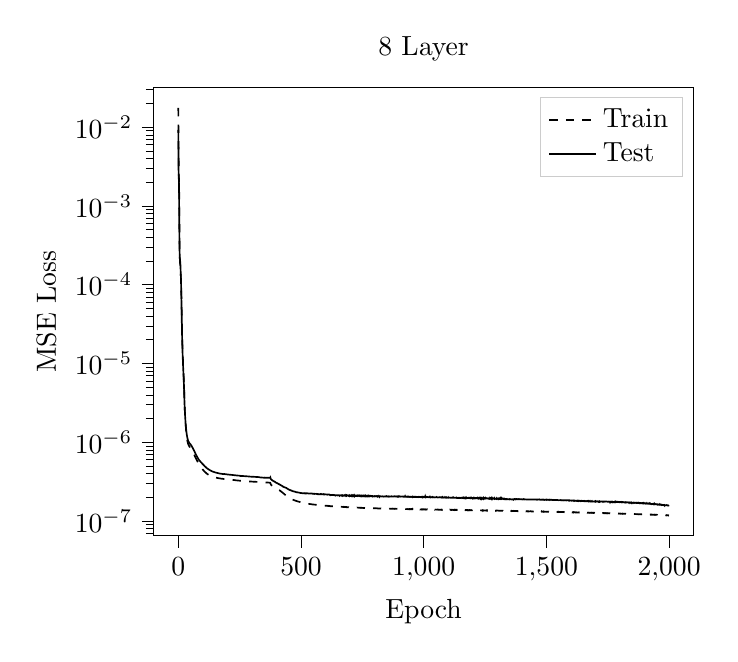
\begin{tikzpicture}

\begin{axis}[
legend cell align={left},
legend style={fill opacity=0.8, draw opacity=1, text opacity=1, draw=white!80!black},
log basis y={10},
tick align=outside,
tick pos=left,
title={8 Layer},
x grid style={white!69.0196078431373!black},
xlabel={Epoch},
xmin=-99.95, xmax=2098.95,
xtick style={color=black},
y grid style={white!69.0196078431373!black},
ylabel={MSE Loss},
ymin=6.47765029335508e-08, ymax=0.0318082202477323,
ymode=log,
ytick style={color=black}
]
\addplot [semithick, black, dashed]
table {%
0 0.0175328296050429
1 0.00526908103376627
2 0.0024811453698203
3 0.0020657035713084
4 0.00106903264287394
5 0.000353904425603105
6 0.000218746372745954
7 0.000189798295497894
8 0.000178016446661786
9 0.000159623949104571
10 0.000136344930841005
11 0.000113073929911479
12 8.84419990870811e-05
13 6.2893814065319e-05
14 4.27583082764613e-05
15 2.92383841242554e-05
16 2.10352017566038e-05
17 1.61476924668023e-05
18 1.30475415135152e-05
19 1.08516150257856e-05
20 9.16441520030276e-06
21 7.80614999439422e-06
22 6.68636070122375e-06
23 5.67973846887071e-06
24 4.59834968637551e-06
25 3.55384452848284e-06
26 2.82646348415483e-06
27 2.36879455329131e-06
28 2.06056119333198e-06
29 1.83083022565711e-06
30 1.64863851436792e-06
31 1.50096731364613e-06
32 1.38044920056757e-06
33 1.28160291140489e-06
34 1.20055532232755e-06
35 1.13477372232751e-06
36 1.08220113452262e-06
37 1.03955213090501e-06
38 1.00530486443517e-06
39 9.77610424797604e-07
40 9.54024540931186e-07
41 9.35144095763008e-07
42 9.20161763190208e-07
43 9.06661032530565e-07
44 8.95124449471041e-07
45 8.84884205675007e-07
46 8.75485176464963e-07
47 8.67158681160163e-07
48 8.58861131064259e-07
49 8.49627589815327e-07
50 8.40432371091993e-07
51 8.30126947960252e-07
52 8.20814274163695e-07
53 8.11791434074394e-07
54 8.02703816390249e-07
55 7.93062617361784e-07
56 7.83371090648188e-07
57 7.73359274489849e-07
58 7.63606251297233e-07
59 7.53800127654358e-07
60 7.43594718784379e-07
61 7.33601759947078e-07
62 7.23426322423393e-07
63 7.13205591125643e-07
64 7.0250906480851e-07
65 6.91736627373984e-07
66 6.8141382240583e-07
67 6.70850326486061e-07
68 6.60704809689605e-07
69 6.50622080343055e-07
70 6.40856266045375e-07
71 6.30526041106805e-07
72 6.21069840335053e-07
73 6.12328547347829e-07
74 6.03472821694595e-07
75 5.94954458605912e-07
76 5.86979994452008e-07
77 5.79193048764637e-07
78 5.7177413894749e-07
79 5.64665561554989e-07
80 5.5709349710753e-07
81 5.49923466209634e-07
82 5.4292612233553e-07
83 5.36258046594185e-07
84 5.29824090421016e-07
85 5.23648571146396e-07
86 5.17685902934772e-07
87 5.11069741804704e-07
88 5.05491432136296e-07
89 5.00108199872784e-07
90 4.9472347799906e-07
91 4.89829184886048e-07
92 4.84885792644718e-07
93 4.79588366886219e-07
94 4.74725679453059e-07
95 4.70136502784158e-07
96 4.65507118178721e-07
97 4.61073159385705e-07
98 4.56837894091677e-07
99 4.52725050351432e-07
100 4.48878952340692e-07
101 4.45040633863414e-07
102 4.41461416315292e-07
103 4.3791901580903e-07
104 4.34556433205557e-07
105 4.31228226531744e-07
106 4.28184232518447e-07
107 4.25006038128117e-07
108 4.22162241264346e-07
109 4.19006269950728e-07
110 4.16332390557272e-07
111 4.13429551699096e-07
112 4.10771487253214e-07
113 4.07942185475463e-07
114 4.05494348484581e-07
115 4.02784749738316e-07
116 4.00286914086223e-07
117 3.97965309545611e-07
118 3.95838657212266e-07
119 3.94044673285521e-07
120 3.92032634195516e-07
121 3.89872294590532e-07
122 3.88192757952766e-07
123 3.86300660608185e-07
124 3.84687878252521e-07
125 3.82859825634796e-07
126 3.81259326559302e-07
127 3.79667921393434e-07
128 3.7808499344294e-07
129 3.76785870017216e-07
130 3.75500086406078e-07
131 3.74170697980958e-07
132 3.72888158608475e-07
133 3.71877083168215e-07
134 3.70665013264215e-07
135 3.69590087345273e-07
136 3.68685641021216e-07
137 3.67684927169876e-07
138 3.66738080046503e-07
139 3.65638564375104e-07
140 3.64869017559499e-07
141 3.63847870005429e-07
142 3.62878456101612e-07
143 3.6201422052784e-07
144 3.61405104754908e-07
145 3.60622909369113e-07
146 3.59861233491188e-07
147 3.59144117268784e-07
148 3.58545277876487e-07
149 3.57887540502588e-07
150 3.57249293870154e-07
151 3.56527215444658e-07
152 3.56127539916429e-07
153 3.55544571846167e-07
154 3.55036048958368e-07
155 3.54611293843732e-07
156 3.54111535571633e-07
157 3.53505102594909e-07
158 3.52848333747602e-07
159 3.52149421956938e-07
160 3.51732665635041e-07
161 3.51205987101366e-07
162 3.50830501929522e-07
163 3.50395613395449e-07
164 3.49923345510206e-07
165 3.49431554028001e-07
166 3.48941883544285e-07
167 3.48522583536237e-07
168 3.48186346826651e-07
169 3.47681064312155e-07
170 3.47169353645427e-07
171 3.46804226069253e-07
172 3.46499707390535e-07
173 3.46075071732344e-07
174 3.45697041879589e-07
175 3.45525421082016e-07
176 3.45072367338162e-07
177 3.44646222188771e-07
178 3.44242588923294e-07
179 3.43962912864981e-07
180 3.43637114866624e-07
181 3.43373919974965e-07
182 3.43108959057759e-07
183 3.42715657879467e-07
184 3.42481556671714e-07
185 3.42151080772624e-07
186 3.41881741704242e-07
187 3.41519302025972e-07
188 3.41339824942111e-07
189 3.41067975909937e-07
190 3.4067830320339e-07
191 3.40474474853636e-07
192 3.40126796245954e-07
193 3.39870608186743e-07
194 3.39526693821313e-07
195 3.39317672114703e-07
196 3.38837426596683e-07
197 3.38705993669919e-07
198 3.38400550219831e-07
199 3.38316658016424e-07
200 3.37989257033655e-07
201 3.37688488230015e-07
202 3.37399379517933e-07
203 3.37125496955082e-07
204 3.36861192039351e-07
205 3.36608914466296e-07
206 3.36245998028062e-07
207 3.36085985836121e-07
208 3.35786493664614e-07
209 3.35561873896495e-07
210 3.35280411874805e-07
211 3.35142199233474e-07
212 3.34837603901406e-07
213 3.34593124080129e-07
214 3.34344883739845e-07
215 3.34137826051517e-07
216 3.33863607160367e-07
217 3.33455762159929e-07
218 3.3319723637959e-07
219 3.33105943873591e-07
220 3.32865009873728e-07
221 3.3264331553795e-07
222 3.32412592904063e-07
223 3.32070278993513e-07
224 3.31828170644144e-07
225 3.31597699712916e-07
226 3.31352910691862e-07
227 3.31146232390722e-07
228 3.31056747498337e-07
229 3.30603054095491e-07
230 3.30301297225333e-07
231 3.30080206424554e-07
232 3.29558580105527e-07
233 3.2933908271815e-07
234 3.29115459202001e-07
235 3.28839234775558e-07
236 3.28580431173009e-07
237 3.28323732759372e-07
238 3.2807043584171e-07
239 3.27747669892631e-07
240 3.27464948348677e-07
241 3.27200872433764e-07
242 3.26998274999823e-07
243 3.26803397669551e-07
244 3.26481064050199e-07
245 3.26303489700308e-07
246 3.26089179225164e-07
247 3.25924068953043e-07
248 3.25714338714533e-07
249 3.25468668862072e-07
250 3.25018146298817e-07
251 3.24853583165918e-07
252 3.24682733442216e-07
253 3.24474176309764e-07
254 3.24312471967403e-07
255 3.24107295426757e-07
256 3.23898819900137e-07
257 3.23801022510395e-07
258 3.23574237739876e-07
259 3.23386136919623e-07
260 3.23154673509407e-07
261 3.22951625179257e-07
262 3.22757495133885e-07
263 3.22559811543499e-07
264 3.22383646050639e-07
265 3.22176338926283e-07
266 3.21986999956891e-07
267 3.21799536330047e-07
268 3.21615479748516e-07
269 3.2131524605461e-07
270 3.21098087837868e-07
271 3.20949953959371e-07
272 3.20814928393531e-07
273 3.20597945510315e-07
274 3.20427085533481e-07
275 3.20249152103713e-07
276 3.2012393730696e-07
277 3.1993017118026e-07
278 3.19784813910928e-07
279 3.19583986197358e-07
280 3.1947266468535e-07
281 3.19318750968023e-07
282 3.19150666001633e-07
283 3.18975156424983e-07
284 3.18834318278505e-07
285 3.18683478894854e-07
286 3.18506897286852e-07
287 3.1842577485719e-07
288 3.18197053516656e-07
289 3.18177214133186e-07
290 3.17996098942785e-07
291 3.1795230303544e-07
292 3.17774085651479e-07
293 3.17555649353096e-07
294 3.17525105934635e-07
295 3.17360777685849e-07
296 3.17117739221828e-07
297 3.17186909256861e-07
298 3.16859379964285e-07
299 3.16811100702807e-07
300 3.16564827016919e-07
301 3.16546802324069e-07
302 3.16414311839708e-07
303 3.16191319463144e-07
304 3.16013029326712e-07
305 3.15986825370374e-07
306 3.1582280825404e-07
307 3.1556253458831e-07
308 3.15551690242444e-07
309 3.15488802044683e-07
310 3.15251602359012e-07
311 3.1524402550076e-07
312 3.14834048296575e-07
313 3.1502463754407e-07
314 3.14750351606108e-07
315 3.14771214370069e-07
316 3.1452549758626e-07
317 3.14477254761414e-07
318 3.14290501833625e-07
319 3.14295230836592e-07
320 3.13890693590224e-07
321 3.14136570423784e-07
322 3.1390767691164e-07
323 3.13873346939886e-07
324 3.13628105161001e-07
325 3.136031422315e-07
326 3.13384845625819e-07
327 3.13368351783083e-07
328 3.13223696586817e-07
329 3.13095284589338e-07
330 3.13103127901115e-07
331 3.12966587756591e-07
332 3.12709218896146e-07
333 3.12110520169995e-07
334 3.12222397674589e-07
335 3.12361991092303e-07
336 3.12118241708959e-07
337 3.11978893279274e-07
338 3.11915353471193e-07
339 3.11790699221604e-07
340 3.11596081047583e-07
341 3.11180611667794e-07
342 3.11583242257996e-07
343 3.11007668919672e-07
344 3.10850106806981e-07
345 3.10863525172067e-07
346 3.10767936177569e-07
347 3.10908169538493e-07
348 3.10390755146273e-07
349 3.10416143840087e-07
350 3.10616684522813e-07
351 3.10328716629726e-07
352 3.0965765838431e-07
353 3.09850993204464e-07
354 3.09702653474631e-07
355 3.09501027999204e-07
356 3.09061599175209e-07
357 3.09046005845914e-07
358 3.08902529347677e-07
359 3.08754219012997e-07
360 3.08652673965071e-07
361 3.0852893022626e-07
362 3.08412155753501e-07
363 3.08110915753446e-07
364 3.08090832113805e-07
365 3.07928383392664e-07
366 3.07783716692711e-07
367 3.07759822206322e-07
368 3.07536354554827e-07
369 3.07389559360161e-07
370 3.0712789580889e-07
371 3.07107941253548e-07
372 3.06821632392484e-07
373 3.06744424726446e-07
374 3.06417181519691e-07
375 3.05259786543388e-07
376 2.96313256789915e-07
377 2.90663783623302e-07
378 2.87804450067597e-07
379 2.85735052990788e-07
380 2.84615552835987e-07
381 2.83525199733958e-07
382 2.82446022225713e-07
383 2.81321543695867e-07
384 2.80254445300443e-07
385 2.7920743795562e-07
386 2.78225404251486e-07
387 2.77090234497734e-07
388 2.76221330814508e-07
389 2.75151829292497e-07
390 2.74080892651796e-07
391 2.72749642924452e-07
392 2.71503182730726e-07
393 2.70786939665868e-07
394 2.69418694927026e-07
395 2.68065543103546e-07
396 2.66677770433432e-07
397 2.65513972514952e-07
398 2.64282750272571e-07
399 2.62921956583284e-07
400 2.61887793861604e-07
401 2.60402524808967e-07
402 2.59187077418233e-07
403 2.58047188673061e-07
404 2.56683215951625e-07
405 2.55712748042924e-07
406 2.54107455099017e-07
407 2.53149617108761e-07
408 2.51396610721599e-07
409 2.50224179580982e-07
410 2.48511859005873e-07
411 2.47515977186197e-07
412 2.46467274273243e-07
413 2.44899058344572e-07
414 2.43662102086262e-07
415 2.42160927925283e-07
416 2.40837991377418e-07
417 2.39876552527107e-07
418 2.38471986328648e-07
419 2.36897201752129e-07
420 2.35599923733787e-07
421 2.34318138772949e-07
422 2.33158340222417e-07
423 2.31924687582818e-07
424 2.30379069428466e-07
425 2.29331601715899e-07
426 2.27478731481767e-07
427 2.26122672451368e-07
428 2.24842304703543e-07
429 2.23502054168989e-07
430 2.22350452716569e-07
431 2.21158989312187e-07
432 2.19953135321305e-07
433 2.18591989678885e-07
434 2.16939178685038e-07
435 2.15723278444102e-07
436 2.14631776202623e-07
437 2.13478038858739e-07
438 2.12388505580918e-07
439 2.11266726964254e-07
440 2.10094492594237e-07
441 2.08973344783203e-07
442 2.07528438195936e-07
443 2.06402683680551e-07
444 2.05239006199065e-07
445 2.04158008912714e-07
446 2.03251472335353e-07
447 2.02277326174283e-07
448 2.01125351324549e-07
449 2.00188082445152e-07
450 1.9919553130876e-07
451 1.98251505693747e-07
452 1.97417034669911e-07
453 1.96545381626834e-07
454 1.95746966497268e-07
455 1.95005100252388e-07
456 1.93978864757582e-07
457 1.93105879425559e-07
458 1.92514951393719e-07
459 1.91637039471004e-07
460 1.91000602328018e-07
461 1.90360802442058e-07
462 1.89602468800842e-07
463 1.89031795891026e-07
464 1.88446840532208e-07
465 1.87698710270467e-07
466 1.8711253670034e-07
467 1.86705542979837e-07
468 1.85847889987656e-07
469 1.855395490864e-07
470 1.85050495815631e-07
471 1.84422059135159e-07
472 1.837856653637e-07
473 1.83335924596406e-07
474 1.83027025578042e-07
475 1.82589353933338e-07
476 1.81720964455678e-07
477 1.81346602587951e-07
478 1.81113202692984e-07
479 1.80203582523575e-07
480 1.79770764276554e-07
481 1.79706625317522e-07
482 1.78981122033406e-07
483 1.78752520575642e-07
484 1.78582334385169e-07
485 1.77953864849201e-07
486 1.7766869345337e-07
487 1.77351471293719e-07
488 1.76812875736232e-07
489 1.76556565875785e-07
490 1.76516398234128e-07
491 1.76013626244753e-07
492 1.7571760091073e-07
493 1.75353105042575e-07
494 1.74835665283979e-07
495 1.74467691770985e-07
496 1.74291843606511e-07
497 1.7402895901597e-07
498 1.73773440145908e-07
499 1.73715644010031e-07
500 1.73122979084894e-07
501 1.73010420141395e-07
502 1.72502875500413e-07
503 1.72614680799654e-07
504 1.71815977353162e-07
505 1.71901242822514e-07
506 1.71326538904282e-07
507 1.71125863118959e-07
508 1.70994126413859e-07
509 1.70700766794596e-07
510 1.70445046293821e-07
511 1.70266769387695e-07
512 1.69651767969015e-07
513 1.69802070438152e-07
514 1.69355803713245e-07
515 1.69238175175224e-07
516 1.68864305237548e-07
517 1.68296895914466e-07
518 1.68144741152787e-07
519 1.681063232013e-07
520 1.67698545745054e-07
521 1.6727549429163e-07
522 1.67204165720136e-07
523 1.67013722361276e-07
524 1.66806940001152e-07
525 1.66711445601209e-07
526 1.66490661499097e-07
527 1.66064463151372e-07
528 1.6587639635901e-07
529 1.65645136902981e-07
530 1.65257467664048e-07
531 1.65194258968882e-07
532 1.65328429034162e-07
533 1.64852689202633e-07
534 1.64676807820285e-07
535 1.64541102527949e-07
536 1.64355891499213e-07
537 1.64472924332415e-07
538 1.64135093967843e-07
539 1.63986125564008e-07
540 1.63920706143017e-07
541 1.63486246314903e-07
542 1.63418712652685e-07
543 1.63100584771314e-07
544 1.63160991775158e-07
545 1.62823282899183e-07
546 1.62788972254191e-07
547 1.62310552298095e-07
548 1.62172701934082e-07
549 1.62233308088844e-07
550 1.62097987320919e-07
551 1.62025860142023e-07
552 1.61937730943862e-07
553 1.61551917692293e-07
554 1.6153179684153e-07
555 1.61515838158266e-07
556 1.61437829063971e-07
557 1.61197373074629e-07
558 1.61119178898161e-07
559 1.60824594509279e-07
560 1.60852694385483e-07
561 1.60977125005957e-07
562 1.60644661761467e-07
563 1.60562388401786e-07
564 1.60366760141528e-07
565 1.59942062417429e-07
566 1.59711742838908e-07
567 1.60133456724054e-07
568 1.59939134938725e-07
569 1.59850393622207e-07
570 1.59567545566119e-07
571 1.5941060387803e-07
572 1.59075994730529e-07
573 1.59110882194113e-07
574 1.59025825482217e-07
575 1.59193930166168e-07
576 1.59029426406221e-07
577 1.58960345970627e-07
578 1.58873228158996e-07
579 1.58691118166132e-07
580 1.58621524001035e-07
581 1.58440931521397e-07
582 1.5861286637886e-07
583 1.5840617636087e-07
584 1.58177897191081e-07
585 1.5795649078143e-07
586 1.57878831743119e-07
587 1.578905943731e-07
588 1.57640723230656e-07
589 1.57597480061611e-07
590 1.57342908707392e-07
591 1.56953609554478e-07
592 1.57225426349328e-07
593 1.57105286575643e-07
594 1.56963763622286e-07
595 1.56657359909218e-07
596 1.57128599077794e-07
597 1.56802190403482e-07
598 1.56697919422299e-07
599 1.5667860949975e-07
600 1.56515884235375e-07
601 1.56620291136278e-07
602 1.56279259520886e-07
603 1.56165708197875e-07
604 1.56020669244583e-07
605 1.56240268331942e-07
606 1.55817373048706e-07
607 1.56074017709784e-07
608 1.55637327125646e-07
609 1.5567520441806e-07
610 1.55283701715803e-07
611 1.55519019358508e-07
612 1.55492841116711e-07
613 1.55816570945433e-07
614 1.55335301293746e-07
615 1.55531510671381e-07
616 1.5507815454896e-07
617 1.55146671936279e-07
618 1.54875967719903e-07
619 1.53894253887898e-07
620 1.54305659787468e-07
621 1.54376400409717e-07
622 1.54427602577556e-07
623 1.54235710120076e-07
624 1.54084096209317e-07
625 1.54209941705119e-07
626 1.54026973827825e-07
627 1.54299684020032e-07
628 1.54060457653316e-07
629 1.54000254806164e-07
630 1.5397262653849e-07
631 1.5366859639343e-07
632 1.53862857217746e-07
633 1.53386126168442e-07
634 1.53348138315579e-07
635 1.53683566633589e-07
636 1.5352609095487e-07
637 1.53591393573294e-07
638 1.53002734407437e-07
639 1.5306999547704e-07
640 1.53088535963519e-07
641 1.53293578804892e-07
642 1.52966675685207e-07
643 1.52825601404061e-07
644 1.52772602113771e-07
645 1.52778851997937e-07
646 1.52619541619714e-07
647 1.52712212376116e-07
648 1.52516884270426e-07
649 1.52460694920364e-07
650 1.52448910270664e-07
651 1.52357230309264e-07
652 1.5242117907377e-07
653 1.5209905985003e-07
654 1.52307755726611e-07
655 1.52082216018812e-07
656 1.51867642628645e-07
657 1.52324002300475e-07
658 1.52034879739915e-07
659 1.52062457324575e-07
660 1.51832796557727e-07
661 1.51821761832593e-07
662 1.51722176934044e-07
663 1.51759662635698e-07
664 1.51708611028312e-07
665 1.51362560121271e-07
666 1.5133446582638e-07
667 1.51380364613374e-07
668 1.51449823185601e-07
669 1.51108101338338e-07
670 1.51180538388473e-07
671 1.50782916211512e-07
672 1.51165991443492e-07
673 1.51214464580107e-07
674 1.51761085135149e-07
675 1.50811644701321e-07
676 1.51023055781963e-07
677 1.50726220645936e-07
678 1.5102750061402e-07
679 1.50759341906337e-07
680 1.50863532468293e-07
681 1.5039412832607e-07
682 1.50405019361699e-07
683 1.50687183428033e-07
684 1.50395313138318e-07
685 1.49860707534089e-07
686 1.50543398369507e-07
687 1.49918052457565e-07
688 1.49921526016783e-07
689 1.50214154153616e-07
690 1.50098436261459e-07
691 1.49565287060227e-07
692 1.49665437476187e-07
693 1.50014687090305e-07
694 1.49929010170524e-07
695 1.49439825371189e-07
696 1.49774553186433e-07
697 1.49680220250303e-07
698 1.497078620325e-07
699 1.49463090451718e-07
700 1.49500760201704e-07
701 1.4965748385265e-07
702 1.49425968256622e-07
703 1.49092031882958e-07
704 1.49379718401121e-07
705 1.49784281770593e-07
706 1.49356223158037e-07
707 1.49130759467653e-07
708 1.48976830768532e-07
709 1.49068272978781e-07
710 1.49264540628025e-07
711 1.4917010704707e-07
712 1.49419977461207e-07
713 1.48736793999404e-07
714 1.48965444530802e-07
715 1.48944377855287e-07
716 1.49004637158612e-07
717 1.48904402827554e-07
718 1.48690500225257e-07
719 1.4850534645916e-07
720 1.48886191965403e-07
721 1.48935314744136e-07
722 1.48329525529789e-07
723 1.48342651343114e-07
724 1.48138873964143e-07
725 1.48427777201476e-07
726 1.48268044057431e-07
727 1.48134518688892e-07
728 1.48310625430526e-07
729 1.48065957461085e-07
730 1.48151556441434e-07
731 1.48060626877111e-07
732 1.4802541597092e-07
733 1.47803417629433e-07
734 1.4787964930818e-07
735 1.48006359665942e-07
736 1.4761687753051e-07
737 1.47693905873325e-07
738 1.47604845977867e-07
739 1.47512238822145e-07
740 1.47706481826049e-07
741 1.47676154170995e-07
742 1.46773032945191e-07
743 1.47055220313774e-07
744 1.47239715392544e-07
745 1.467912592652e-07
746 1.47049525299536e-07
747 1.47205613501455e-07
748 1.47109882039587e-07
749 1.4667980613936e-07
750 1.46820244534496e-07
751 1.46917181776729e-07
752 1.46934573837854e-07
753 1.46922250465309e-07
754 1.46629619326433e-07
755 1.46714902022893e-07
756 1.46811325457463e-07
757 1.46594789793397e-07
758 1.46552674767264e-07
759 1.46794158258245e-07
760 1.46406611559513e-07
761 1.46276465741835e-07
762 1.46520066905964e-07
763 1.46337387764817e-07
764 1.46368378977968e-07
765 1.46322530774512e-07
766 1.46444433365645e-07
767 1.46170982674221e-07
768 1.46035282174495e-07
769 1.46347738876784e-07
770 1.45868453255815e-07
771 1.45995072564631e-07
772 1.4621667817849e-07
773 1.45996149388594e-07
774 1.45838359781436e-07
775 1.46086144560797e-07
776 1.45816849595803e-07
777 1.45792429265157e-07
778 1.4566305859276e-07
779 1.46017009416966e-07
780 1.45877792149918e-07
781 1.45809088923698e-07
782 1.45412859740901e-07
783 1.45728202642914e-07
784 1.45793485817336e-07
785 1.45572990955856e-07
786 1.45507330024941e-07
787 1.45483349449194e-07
788 1.45378579937017e-07
789 1.45243717270205e-07
790 1.45138936225919e-07
791 1.45445496556817e-07
792 1.4537288086558e-07
793 1.45323052233692e-07
794 1.45249136412673e-07
795 1.44959458381777e-07
796 1.45310082043437e-07
797 1.45089904361129e-07
798 1.44886737540872e-07
799 1.45202101947461e-07
800 1.45081607684006e-07
801 1.45068235003265e-07
802 1.45047729315451e-07
803 1.44639789915857e-07
804 1.44681112377754e-07
805 1.45097899459046e-07
806 1.44912972412925e-07
807 1.44757418407693e-07
808 1.44969247070748e-07
809 1.44877304595781e-07
810 1.45066319774401e-07
811 1.44526176367066e-07
812 1.44770261883309e-07
813 1.44676769728846e-07
814 1.44596687665199e-07
815 1.44527480813394e-07
816 1.44417752558468e-07
817 1.44684981730592e-07
818 1.44646610436894e-07
819 1.44546390689726e-07
820 1.44043759831902e-07
821 1.43988481575263e-07
822 1.44454864035026e-07
823 1.44367983928362e-07
824 1.44315122295069e-07
825 1.44514851303512e-07
826 1.44211226373869e-07
827 1.44078816024518e-07
828 1.44293243820925e-07
829 1.44206716939266e-07
830 1.44275118252324e-07
831 1.44198291060604e-07
832 1.43960377940289e-07
833 1.44308390385817e-07
834 1.43741077277326e-07
835 1.43910124183577e-07
836 1.44126620742924e-07
837 1.44111164065208e-07
838 1.4420608047061e-07
839 1.43975314230715e-07
840 1.44012661287718e-07
841 1.43980029530866e-07
842 1.43928399559456e-07
843 1.43848968185978e-07
844 1.43690816585718e-07
845 1.44003668232529e-07
846 1.43679508973094e-07
847 1.43783171800749e-07
848 1.43928508908431e-07
849 1.43680912799482e-07
850 1.44121392462893e-07
851 1.43895006939232e-07
852 1.43512517407629e-07
853 1.43355135772794e-07
854 1.43424258631342e-07
855 1.43617109703342e-07
856 1.43774829503229e-07
857 1.43508643439816e-07
858 1.43625492381005e-07
859 1.43168517407588e-07
860 1.43556524633937e-07
861 1.43369579628683e-07
862 1.4350661416529e-07
863 1.43150451556551e-07
864 1.43568707436259e-07
865 1.4335619835748e-07
866 1.43229341304618e-07
867 1.43312628949843e-07
868 1.43442354200829e-07
869 1.43290071264346e-07
870 1.43341870831648e-07
871 1.43120179540546e-07
872 1.43148483605415e-07
873 1.42917345435478e-07
874 1.43662633611541e-07
875 1.42980072517673e-07
876 1.42999039763225e-07
877 1.43008041625592e-07
878 1.43002305986073e-07
879 1.43241044330722e-07
880 1.42978790144355e-07
881 1.43165590785088e-07
882 1.42598846199604e-07
883 1.43180287722089e-07
884 1.42780469488457e-07
885 1.42780916569052e-07
886 1.42969993397912e-07
887 1.42703800605659e-07
888 1.42895849410962e-07
889 1.42793996602109e-07
890 1.42831420259171e-07
891 1.42718856707802e-07
892 1.42954531902717e-07
893 1.42701163781567e-07
894 1.42444937743846e-07
895 1.4261761233314e-07
896 1.42605217273939e-07
897 1.42689636913218e-07
898 1.42392338929653e-07
899 1.4255365073268e-07
900 1.42336699212819e-07
901 1.42699972283111e-07
902 1.42488840616295e-07
903 1.4252937375403e-07
904 1.4202959576437e-07
905 1.425743420711e-07
906 1.4243057094987e-07
907 1.42474533404879e-07
908 1.42089733259354e-07
909 1.42119609343183e-07
910 1.42345393491894e-07
911 1.42107149244453e-07
912 1.42211034706463e-07
913 1.4240851080416e-07
914 1.4221744854126e-07
915 1.42267661875195e-07
916 1.42202555696969e-07
917 1.41925924797448e-07
918 1.41971158406307e-07
919 1.4210136470183e-07
920 1.42300199058809e-07
921 1.4193852898714e-07
922 1.42140022891368e-07
923 1.42676953529985e-07
924 1.42855565659517e-07
925 1.42496458355623e-07
926 1.42077827710807e-07
927 1.4173500014536e-07
928 1.41774210817402e-07
929 1.4185019106705e-07
930 1.41530856794247e-07
931 1.41516090682359e-07
932 1.4148874922526e-07
933 1.41717627791138e-07
934 1.41738756664012e-07
935 1.42321595205885e-07
936 1.41502772880386e-07
937 1.41590681753456e-07
938 1.4135556979511e-07
939 1.41424335893703e-07
940 1.4142615881596e-07
941 1.42026300974152e-07
942 1.41953662016192e-07
943 1.41265155992443e-07
944 1.42225362758097e-07
945 1.4185230777386e-07
946 1.4118388476092e-07
947 1.41045869781919e-07
948 1.40988311517987e-07
949 1.42108610312164e-07
950 1.42266998906848e-07
951 1.41178457901958e-07
952 1.40924142737475e-07
953 1.4084296048722e-07
954 1.41030333150383e-07
955 1.42312434267211e-07
956 1.40815855555587e-07
957 1.41811550495419e-07
958 1.41584311652565e-07
959 1.40938345623454e-07
960 1.40837006021854e-07
961 1.41598450394298e-07
962 1.41160173079413e-07
963 1.40844735707191e-07
964 1.41018507303414e-07
965 1.40989900536681e-07
966 1.41357851422441e-07
967 1.41701209749101e-07
968 1.40556913073908e-07
969 1.41622540972719e-07
970 1.40686534969348e-07
971 1.4053291606686e-07
972 1.40638144088712e-07
973 1.41467908843396e-07
974 1.40740276282969e-07
975 1.40685108373617e-07
976 1.40603891324531e-07
977 1.40684053398843e-07
978 1.41419389557029e-07
979 1.41598929936038e-07
980 1.41155748718091e-07
981 1.4127184632784e-07
982 1.41115515578605e-07
983 1.41157341086995e-07
984 1.41093482294963e-07
985 1.40244625491448e-07
986 1.40437968127571e-07
987 1.40473355934034e-07
988 1.40752477928885e-07
989 1.40687068828527e-07
990 1.40017776338652e-07
991 1.41015269630174e-07
992 1.40835331620792e-07
993 1.40545132662595e-07
994 1.41174887165363e-07
995 1.41119856710503e-07
996 1.40208206119041e-07
997 1.40931780023834e-07
998 1.4022020828719e-07
999 1.40919137169959e-07
1000 1.40721628962837e-07
1001 1.40827392534959e-07
1002 1.40272580253509e-07
1003 1.39982767475288e-07
1004 1.4001712857592e-07
1005 1.41045355317004e-07
1006 1.40934940986881e-07
1007 1.40801237918708e-07
1008 1.40705775212524e-07
1009 1.39573305421692e-07
1010 1.40005285206968e-07
1011 1.39985599552972e-07
1012 1.3998350164357e-07
1013 1.40217492749173e-07
1014 1.40933221167927e-07
1015 1.40469146966637e-07
1016 1.39870673319109e-07
1017 1.40242820979353e-07
1018 1.40717302322457e-07
1019 1.39738414247859e-07
1020 1.40684658493484e-07
1021 1.39640350049319e-07
1022 1.3976327009857e-07
1023 1.40896664014178e-07
1024 1.4003093021131e-07
1025 1.40633622720543e-07
1026 1.40413035932596e-07
1027 1.40312370913165e-07
1028 1.39787127331203e-07
1029 1.40090054060238e-07
1030 1.40548668227325e-07
1031 1.39413021557289e-07
1032 1.39588993896211e-07
1033 1.40005150228717e-07
1034 1.39753148697963e-07
1035 1.39596208203585e-07
1036 1.3951229968967e-07
1037 1.40408136896752e-07
1038 1.39835310108083e-07
1039 1.40405866954296e-07
1040 1.40260662099934e-07
1041 1.39776692630988e-07
1042 1.40046229791579e-07
1043 1.40275582459992e-07
1044 1.39946306664029e-07
1045 1.39301153780025e-07
1046 1.39497414391343e-07
1047 1.39598235257665e-07
1048 1.39690142994198e-07
1049 1.39807074788223e-07
1050 1.39737415786101e-07
1051 1.39700335019199e-07
1052 1.39594883965088e-07
1053 1.3950548950703e-07
1054 1.39740799987464e-07
1055 1.39295418208008e-07
1056 1.3973811096335e-07
1057 1.40247204662103e-07
1058 1.39764830574762e-07
1059 1.39799569627286e-07
1060 1.39192969097479e-07
1061 1.39496986072629e-07
1062 1.39270260721247e-07
1063 1.39414751853195e-07
1064 1.39368439160847e-07
1065 1.39430535600837e-07
1066 1.39370543582373e-07
1067 1.39014138344606e-07
1068 1.3903848970287e-07
1069 1.39036954866611e-07
1070 1.38956512998334e-07
1071 1.39268774670853e-07
1072 1.39314872974694e-07
1073 1.38759399373356e-07
1074 1.3974047739751e-07
1075 1.38765189806378e-07
1076 1.39840884134657e-07
1077 1.39689777260088e-07
1078 1.3940588398853e-07
1079 1.39469934833159e-07
1080 1.39180955024187e-07
1081 1.3941563042863e-07
1082 1.38784151552329e-07
1083 1.39607714665146e-07
1084 1.38701271541919e-07
1085 1.39057623346872e-07
1086 1.39424572637381e-07
1087 1.39112138135999e-07
1088 1.38356904830772e-07
1089 1.38704682374424e-07
1090 1.39570322634341e-07
1091 1.39438522612778e-07
1092 1.39256844970959e-07
1093 1.38886850859166e-07
1094 1.39106300593994e-07
1095 1.38832809213341e-07
1096 1.38724195892337e-07
1097 1.38557934619143e-07
1098 1.39467144848027e-07
1099 1.39032704108644e-07
1100 1.38914165511039e-07
1101 1.39027073945641e-07
1102 1.386054461463e-07
1103 1.3844797469531e-07
1104 1.38298065451181e-07
1105 1.38539775452529e-07
1106 1.38387163005405e-07
1107 1.39363646990631e-07
1108 1.39057628707917e-07
1109 1.3864583001677e-07
1110 1.38458758947024e-07
1111 1.38663611714662e-07
1112 1.38217955239384e-07
1113 1.39053501012398e-07
1114 1.38698975955975e-07
1115 1.38392806523058e-07
1116 1.38454945290079e-07
1117 1.38877848510077e-07
1118 1.38484777625791e-07
1119 1.3804813632845e-07
1120 1.384317418065e-07
1121 1.38236011867576e-07
1122 1.38729906922208e-07
1123 1.3860993410475e-07
1124 1.38744956498016e-07
1125 1.37916542406913e-07
1126 1.39003695924345e-07
1127 1.38235406847542e-07
1128 1.38581443195562e-07
1129 1.38985475299336e-07
1130 1.38347661192029e-07
1131 1.3873075161186e-07
1132 1.38244267315457e-07
1133 1.38409569611753e-07
1134 1.38766601232021e-07
1135 1.3816313969528e-07
1136 1.3874601235031e-07
1137 1.38215914162743e-07
1138 1.38433437424368e-07
1139 1.38305761815616e-07
1140 1.3816990382054e-07
1141 1.38154227816045e-07
1142 1.3817131157623e-07
1143 1.37816663091428e-07
1144 1.37279932747703e-07
1145 1.38278222902244e-07
1146 1.38441186155802e-07
1147 1.38293754037733e-07
1148 1.38114186285065e-07
1149 1.38382457134156e-07
1150 1.38121935648883e-07
1151 1.38317404871913e-07
1152 1.3726398281122e-07
1153 1.38135500790781e-07
1154 1.37828834432696e-07
1155 1.37260662473437e-07
1156 1.37698246579276e-07
1157 1.38406393155321e-07
1158 1.38022530450144e-07
1159 1.38276047778163e-07
1160 1.37411542546317e-07
1161 1.38349900112189e-07
1162 1.37902236627241e-07
1163 1.38121288390636e-07
1164 1.37785931336509e-07
1165 1.38097032252205e-07
1166 1.38174561051585e-07
1167 1.38032484766626e-07
1168 1.37848963614573e-07
1169 1.3723605952265e-07
1170 1.37956863941469e-07
1171 1.37981708157042e-07
1172 1.37641746089656e-07
1173 1.37537446441627e-07
1174 1.37715307477748e-07
1175 1.3802467366375e-07
1176 1.37435121121854e-07
1177 1.37773701698762e-07
1178 1.37598071777489e-07
1179 1.37826937510965e-07
1180 1.3687629511594e-07
1181 1.3763023151725e-07
1182 1.37472484304624e-07
1183 1.36806704883696e-07
1184 1.37347097012963e-07
1185 1.36806844061255e-07
1186 1.37831803662891e-07
1187 1.37434617570875e-07
1188 1.3769349364523e-07
1189 1.37824878567727e-07
1190 1.37278291237664e-07
1191 1.37285638022178e-07
1192 1.37537405553445e-07
1193 1.37367708799019e-07
1194 1.37173955799597e-07
1195 1.3737849220874e-07
1196 1.37694570426561e-07
1197 1.37204371121413e-07
1198 1.37134707571818e-07
1199 1.37665647152119e-07
1200 1.36953320932776e-07
1201 1.37370643354728e-07
1202 1.37206181204164e-07
1203 1.37008231114066e-07
1204 1.37595916893218e-07
1205 1.36808668081301e-07
1206 1.37278483379077e-07
1207 1.37148173621426e-07
1208 1.37073568943435e-07
1209 1.36834813723397e-07
1210 1.37074007465543e-07
1211 1.37088900583393e-07
1212 1.37079231969039e-07
1213 1.36705124127445e-07
1214 1.37048769406789e-07
1215 1.37013939077946e-07
1216 1.37600832001539e-07
1217 1.36949269979425e-07
1218 1.37130617353876e-07
1219 1.37060159055125e-07
1220 1.37085094007006e-07
1221 1.36812554405452e-07
1222 1.37024799300889e-07
1223 1.36926175436258e-07
1224 1.36370574427502e-07
1225 1.36324622825867e-07
1226 1.36892710990821e-07
1227 1.36951245121253e-07
1228 1.36814091263204e-07
1229 1.3654238679095e-07
1230 1.37057469043356e-07
1231 1.36701299577879e-07
1232 1.3652721672841e-07
1233 1.3685295296284e-07
1234 1.36608417133033e-07
1235 1.36408859674475e-07
1236 1.36091057672871e-07
1237 1.3619267259557e-07
1238 1.36285035583938e-07
1239 1.36530719178296e-07
1240 1.37105354312439e-07
1241 1.35431814818787e-07
1242 1.3684890741672e-07
1243 1.3663633738048e-07
1244 1.36236742655171e-07
1245 1.36506144674087e-07
1246 1.36222827489263e-07
1247 1.36451787916769e-07
1248 1.36626566039411e-07
1249 1.36391327373531e-07
1250 1.36479924456978e-07
1251 1.35830370680878e-07
1252 1.35618493807499e-07
1253 1.35934234069879e-07
1254 1.36055470630225e-07
1255 1.36669150702318e-07
1256 1.36405847417365e-07
1257 1.36319522386685e-07
1258 1.35291791945491e-07
1259 1.36776484112033e-07
1260 1.36283775297841e-07
1261 1.36266703815835e-07
1262 1.35965188928111e-07
1263 1.36535373140845e-07
1264 1.35733946944327e-07
1265 1.3617216602313e-07
1266 1.36112452828741e-07
1267 1.36237589192234e-07
1268 1.36063071604298e-07
1269 1.35476228248166e-07
1270 1.36250667537752e-07
1271 1.35881678090755e-07
1272 1.35979288831578e-07
1273 1.36238702118874e-07
1274 1.35648261981203e-07
1275 1.35880330763172e-07
1276 1.35914717418473e-07
1277 1.36027546457029e-07
1278 1.35853306886702e-07
1279 1.35285529214713e-07
1280 1.35539836794152e-07
1281 1.35683692555233e-07
1282 1.36025817489838e-07
1283 1.35835172550003e-07
1284 1.35056589666505e-07
1285 1.35935776850005e-07
1286 1.35621498060345e-07
1287 1.35414710101145e-07
1288 1.3520019967217e-07
1289 1.35646540183387e-07
1290 1.35784820663787e-07
1291 1.35338610498081e-07
1292 1.35329451261157e-07
1293 1.3545026487094e-07
1294 1.34593553923423e-07
1295 1.35693883191124e-07
1296 1.35603320561728e-07
1297 1.35862542691711e-07
1298 1.35825982674476e-07
1299 1.35838342881556e-07
1300 1.35632517498152e-07
1301 1.35736545058052e-07
1302 1.35440545069088e-07
1303 1.35403063097783e-07
1304 1.35380686813846e-07
1305 1.35425861454763e-07
1306 1.35607733412257e-07
1307 1.35032257166046e-07
1308 1.35039564661099e-07
1309 1.35352815490819e-07
1310 1.35184736461014e-07
1311 1.35230940468745e-07
1312 1.35324441441043e-07
1313 1.34647033465995e-07
1314 1.34791245049115e-07
1315 1.35218023384454e-07
1316 1.35195162897617e-07
1317 1.35294213944093e-07
1318 1.3488464167466e-07
1319 1.35344892409961e-07
1320 1.34881540162723e-07
1321 1.35190767682758e-07
1322 1.35402391805428e-07
1323 1.34437263884735e-07
1324 1.35373538814321e-07
1325 1.3493949830945e-07
1326 1.34989981521727e-07
1327 1.3497682837027e-07
1328 1.34721640101532e-07
1329 1.34469346654953e-07
1330 1.34818239921231e-07
1331 1.33841995442197e-07
1332 1.34700803222643e-07
1333 1.3439547620564e-07
1334 1.34984121679338e-07
1335 1.34795854503267e-07
1336 1.34525469743352e-07
1337 1.3461953422933e-07
1338 1.34462001998514e-07
1339 1.34843029677256e-07
1340 1.3420433430511e-07
1341 1.34563807471011e-07
1342 1.34867390901405e-07
1343 1.34510761792939e-07
1344 1.34730030342922e-07
1345 1.34435606849337e-07
1346 1.34411263609024e-07
1347 1.34256437316793e-07
1348 1.34782813972834e-07
1349 1.34024590582982e-07
1350 1.34568452995865e-07
1351 1.34362380514119e-07
1352 1.34302472829972e-07
1353 1.34351334761362e-07
1354 1.34335907890915e-07
1355 1.34120713873642e-07
1356 1.34727013193725e-07
1357 1.3408221532174e-07
1358 1.34729800823408e-07
1359 1.33871938110985e-07
1360 1.34318109189735e-07
1361 1.33864743343537e-07
1362 1.33782924415016e-07
1363 1.33831355135783e-07
1364 1.34113517070489e-07
1365 1.34292689914162e-07
1366 1.33977288928833e-07
1367 1.34500697772211e-07
1368 1.33883850152117e-07
1369 1.34232168132797e-07
1370 1.34191160224617e-07
1371 1.33971361943708e-07
1372 1.34148812882984e-07
1373 1.34059907523465e-07
1374 1.34011533003076e-07
1375 1.33912587273244e-07
1376 1.34207291516475e-07
1377 1.33993816298528e-07
1378 1.33813187630949e-07
1379 1.33925051226669e-07
1380 1.33609595302175e-07
1381 1.33904241835125e-07
1382 1.34056787935322e-07
1383 1.33134117795919e-07
1384 1.33370779437314e-07
1385 1.33212562847262e-07
1386 1.33458020300736e-07
1387 1.3342541274497e-07
1388 1.33344620042664e-07
1389 1.33045203249083e-07
1390 1.33173939648401e-07
1391 1.33735852706707e-07
1392 1.33101146182923e-07
1393 1.33628113918149e-07
1394 1.33048745031061e-07
1395 1.3363897600982e-07
1396 1.33286138424893e-07
1397 1.33129509002572e-07
1398 1.33416546312048e-07
1399 1.33238605958042e-07
1400 1.33379363671082e-07
1401 1.32978078468682e-07
1402 1.3356520895158e-07
1403 1.32921508672723e-07
1404 1.33823932376487e-07
1405 1.32866876739968e-07
1406 1.33234917843339e-07
1407 1.33153241058892e-07
1408 1.33098256689834e-07
1409 1.33156855461891e-07
1410 1.32817506489857e-07
1411 1.32931520688828e-07
1412 1.33269521125356e-07
1413 1.33011132493976e-07
1414 1.33485634137287e-07
1415 1.33242297888359e-07
1416 1.33132474370967e-07
1417 1.3259303654678e-07
1418 1.3304268214398e-07
1419 1.33466728897247e-07
1420 1.33002457850751e-07
1421 1.32801221386813e-07
1422 1.33324380179545e-07
1423 1.3274783855266e-07
1424 1.33157652172144e-07
1425 1.3254952354913e-07
1426 1.32873556612623e-07
1427 1.32407889910979e-07
1428 1.32744041508204e-07
1429 1.32378662826227e-07
1430 1.32670230499343e-07
1431 1.32587954393415e-07
1432 1.32656734994185e-07
1433 1.32849608920793e-07
1434 1.32743974827321e-07
1435 1.32634176555513e-07
1436 1.33182105667373e-07
1437 1.32471532481304e-07
1438 1.32415526973517e-07
1439 1.32673556713314e-07
1440 1.32404575865053e-07
1441 1.32716721562787e-07
1442 1.32429709207571e-07
1443 1.32324919132287e-07
1444 1.32314515127518e-07
1445 1.32301039705851e-07
1446 1.3211925281098e-07
1447 1.32657475521825e-07
1448 1.32912559909215e-07
1449 1.32554381384153e-07
1450 1.32347947413791e-07
1451 1.32099213207226e-07
1452 1.32150625326233e-07
1453 1.32160753622657e-07
1454 1.3207741969623e-07
1455 1.31980249019392e-07
1456 1.32116101994484e-07
1457 1.32137307879532e-07
1458 1.32061789404503e-07
1459 1.32048744411861e-07
1460 1.32378337653449e-07
1461 1.32101896774373e-07
1462 1.32699420056781e-07
1463 1.31930627890853e-07
1464 1.32252337969874e-07
1465 1.32622942700777e-07
1466 1.32286355036371e-07
1467 1.32539021823419e-07
1468 1.32651284406649e-07
1469 1.32340801513919e-07
1470 1.32256910539752e-07
1471 1.32004824102694e-07
1472 1.32280205178859e-07
1473 1.32093755226492e-07
1474 1.31662019260403e-07
1475 1.32213106066814e-07
1476 1.31271451138559e-07
1477 1.31864246128544e-07
1478 1.31608354905666e-07
1479 1.30965473260858e-07
1480 1.32271324694955e-07
1481 1.31262430571155e-07
1482 1.31543934809741e-07
1483 1.313864367809e-07
1484 1.31590168670925e-07
1485 1.31592009804393e-07
1486 1.32355213668944e-07
1487 1.31233894322236e-07
1488 1.322243186479e-07
1489 1.31188508561308e-07
1490 1.31564933301576e-07
1491 1.31285795003322e-07
1492 1.31731327115858e-07
1493 1.3135731555991e-07
1494 1.31512092288233e-07
1495 1.31611965763057e-07
1496 1.31706112298957e-07
1497 1.31114311969327e-07
1498 1.31415391560807e-07
1499 1.31099050221906e-07
1500 1.31427122809669e-07
1501 1.31453035884022e-07
1502 1.3128647963967e-07
1503 1.3111958820744e-07
1504 1.31147327294912e-07
1505 1.31227129489986e-07
1506 1.31290460291922e-07
1507 1.30941434587584e-07
1508 1.31656905814737e-07
1509 1.31472641921704e-07
1510 1.30588963141776e-07
1511 1.31188821065109e-07
1512 1.31706080967575e-07
1513 1.31110556782943e-07
1514 1.30758157158795e-07
1515 1.3106696122378e-07
1516 1.31225491454501e-07
1517 1.31034349763581e-07
1518 1.3103017726479e-07
1519 1.30969628866495e-07
1520 1.30797065246213e-07
1521 1.30787288117773e-07
1522 1.30791775951877e-07
1523 1.30976999024313e-07
1524 1.31051221554657e-07
1525 1.30748538129666e-07
1526 1.30839846438136e-07
1527 1.30894191624265e-07
1528 1.30849193311633e-07
1529 1.30806471442924e-07
1530 1.31186622411406e-07
1531 1.30813544863884e-07
1532 1.30370885592868e-07
1533 1.30964306318759e-07
1534 1.3051633526473e-07
1535 1.3060982085733e-07
1536 1.3062497325933e-07
1537 1.3089209088335e-07
1538 1.30859886741774e-07
1539 1.30665071250036e-07
1540 1.30388852678465e-07
1541 1.30435781791505e-07
1542 1.3038937690979e-07
1543 1.30548729455171e-07
1544 1.30223722596412e-07
1545 1.30463539424142e-07
1546 1.30992637611627e-07
1547 1.30539175991373e-07
1548 1.30286821075742e-07
1549 1.30969028202088e-07
1550 1.30108640519211e-07
1551 1.30534399804816e-07
1552 1.305582544191e-07
1553 1.30258834200703e-07
1554 1.30274908006101e-07
1555 1.30317872567787e-07
1556 1.30202957059566e-07
1557 1.30228620776052e-07
1558 1.30101475114941e-07
1559 1.30086796559681e-07
1560 1.30293293448602e-07
1561 1.2986444609453e-07
1562 1.3018359702599e-07
1563 1.30214615438717e-07
1564 1.29875511923672e-07
1565 1.29994600268191e-07
1566 1.3004828747043e-07
1567 1.29831804429159e-07
1568 1.30118920726119e-07
1569 1.2980349151448e-07
1570 1.30118059821882e-07
1571 1.30010312890505e-07
1572 1.29579943731528e-07
1573 1.30007581773839e-07
1574 1.29633749793356e-07
1575 1.30228536164623e-07
1576 1.30193649013677e-07
1577 1.29590583252792e-07
1578 1.29725245866297e-07
1579 1.30004574170783e-07
1580 1.29605912349007e-07
1581 1.30095143621389e-07
1582 1.29633200369739e-07
1583 1.29431262894997e-07
1584 1.29868774312314e-07
1585 1.29622148691055e-07
1586 1.29606173121743e-07
1587 1.29350665538652e-07
1588 1.29556376911921e-07
1589 1.29484209988817e-07
1590 1.29671797054698e-07
1591 1.29224490592605e-07
1592 1.29702454305658e-07
1593 1.29253210268132e-07
1594 1.29577081668941e-07
1595 1.29228094142064e-07
1596 1.29756646185086e-07
1597 1.29241407474723e-07
1598 1.29243841310966e-07
1599 1.29316493936216e-07
1600 1.29171331739286e-07
1601 1.29152005960975e-07
1602 1.29362774728747e-07
1603 1.29053464974049e-07
1604 1.2973606031963e-07
1605 1.28797939900949e-07
1606 1.292929365313e-07
1607 1.28868934151427e-07
1608 1.29265904050158e-07
1609 1.28977175595679e-07
1610 1.29510403507282e-07
1611 1.28456110278563e-07
1612 1.29433031272441e-07
1613 1.28712626203509e-07
1614 1.28916061377993e-07
1615 1.29057485636963e-07
1616 1.28958677031221e-07
1617 1.28673919501665e-07
1618 1.28923699293182e-07
1619 1.28449451679558e-07
1620 1.29111401921733e-07
1621 1.28495435795628e-07
1622 1.28987836760075e-07
1623 1.28698487564805e-07
1624 1.28473070812873e-07
1625 1.28501706306849e-07
1626 1.28262596685857e-07
1627 1.28696789822413e-07
1628 1.28623904696923e-07
1629 1.28384659472403e-07
1630 1.28826351435407e-07
1631 1.28461536736069e-07
1632 1.28665960101415e-07
1633 1.28115977716448e-07
1634 1.28646519687692e-07
1635 1.28333325623231e-07
1636 1.28468673370463e-07
1637 1.28419803250068e-07
1638 1.28151095964313e-07
1639 1.28518776765674e-07
1640 1.27761854844977e-07
1641 1.28458843533963e-07
1642 1.27842088506469e-07
1643 1.28688504545948e-07
1644 1.28137436067988e-07
1645 1.28033213929513e-07
1646 1.28139297540741e-07
1647 1.2777365060046e-07
1648 1.28386569663519e-07
1649 1.27739248984682e-07
1650 1.28065944082323e-07
1651 1.2789484215503e-07
1652 1.28238655840107e-07
1653 1.2774030926721e-07
1654 1.27987645285543e-07
1655 1.27901294991517e-07
1656 1.27665742937211e-07
1657 1.28034646415642e-07
1658 1.27770535438998e-07
1659 1.28071750069125e-07
1660 1.2736325490792e-07
1661 1.27776725353357e-07
1662 1.27459353095105e-07
1663 1.2781280282681e-07
1664 1.27549898106594e-07
1665 1.27953898388711e-07
1666 1.27458225748001e-07
1667 1.27477272538812e-07
1668 1.27502214869679e-07
1669 1.27840303445481e-07
1670 1.27344695510345e-07
1671 1.2779773659588e-07
1672 1.27378690098823e-07
1673 1.27423267638704e-07
1674 1.27738863163529e-07
1675 1.27728986679898e-07
1676 1.27057836525779e-07
1677 1.27538693256213e-07
1678 1.27737066165423e-07
1679 1.2724590301616e-07
1680 1.27389885889784e-07
1681 1.27419158154396e-07
1682 1.26930182634766e-07
1683 1.27623879183858e-07
1684 1.27154275617158e-07
1685 1.27618358977344e-07
1686 1.27124929791833e-07
1687 1.27371926229358e-07
1688 1.26812731377157e-07
1689 1.27139282056987e-07
1690 1.27218484401226e-07
1691 1.26683921443771e-07
1692 1.27419617534485e-07
1693 1.27127938714722e-07
1694 1.26770443650059e-07
1695 1.26936346060091e-07
1696 1.27238350650316e-07
1697 1.26644798047693e-07
1698 1.27171476734134e-07
1699 1.27158263339311e-07
1700 1.26667268503411e-07
1701 1.26758011871786e-07
1702 1.26943203177632e-07
1703 1.26554607881246e-07
1704 1.26810259747145e-07
1705 1.26932658776724e-07
1706 1.26421777608243e-07
1707 1.2673739819391e-07
1708 1.26697367846873e-07
1709 1.26480299435627e-07
1710 1.26809969536623e-07
1711 1.27035903584982e-07
1712 1.26366957513113e-07
1713 1.26592793254332e-07
1714 1.26770064095894e-07
1715 1.26240449798587e-07
1716 1.26640036853587e-07
1717 1.26556261182742e-07
1718 1.26416310795463e-07
1719 1.2641169741201e-07
1720 1.26396524532169e-07
1721 1.26857644250578e-07
1722 1.26102100804104e-07
1723 1.26611768774154e-07
1724 1.26316717345532e-07
1725 1.26042362456502e-07
1726 1.26507704258927e-07
1727 1.26109461305646e-07
1728 1.259183405935e-07
1729 1.26286707903489e-07
1730 1.26402084408284e-07
1731 1.25919816266418e-07
1732 1.26187660194788e-07
1733 1.26308769402783e-07
1734 1.25638530761307e-07
1735 1.26198176705117e-07
1736 1.2606735928955e-07
1737 1.25645882796732e-07
1738 1.26291756597396e-07
1739 1.25750681203129e-07
1740 1.25733389975125e-07
1741 1.25860686726043e-07
1742 1.2616313603786e-07
1743 1.25518500606603e-07
1744 1.25883185095432e-07
1745 1.25860395979061e-07
1746 1.25340654193451e-07
1747 1.26074727837988e-07
1748 1.25575857754967e-07
1749 1.25953525522249e-07
1750 1.25379899493794e-07
1751 1.25843656960001e-07
1752 1.25464775766915e-07
1753 1.25463810007886e-07
1754 1.25469875438711e-07
1755 1.2566498598332e-07
1756 1.25263061672598e-07
1757 1.25437083440261e-07
1758 1.25647742134305e-07
1759 1.25145713862906e-07
1760 1.25421047155072e-07
1761 1.25270755773954e-07
1762 1.25243340477255e-07
1763 1.25492702579777e-07
1764 1.25055630409321e-07
1765 1.25177375423391e-07
1766 1.25128130171959e-07
1767 1.25197676197786e-07
1768 1.25347334147818e-07
1769 1.24891951077899e-07
1770 1.25205880006973e-07
1771 1.25007664649956e-07
1772 1.24870990436676e-07
1773 1.2492002991138e-07
1774 1.25069691989665e-07
1775 1.24701154575746e-07
1776 1.24787520416447e-07
1777 1.24898634002335e-07
1778 1.24526380862022e-07
1779 1.2495914003452e-07
1780 1.24769293034177e-07
1781 1.24856327527567e-07
1782 1.24612163421745e-07
1783 1.24647605659334e-07
1784 1.24934667702803e-07
1785 1.24689066812067e-07
1786 1.24552899283259e-07
1787 1.24575953005746e-07
1788 1.24816830435748e-07
1789 1.24640682901855e-07
1790 1.24436263845951e-07
1791 1.24626855427579e-07
1792 1.24509490433411e-07
1793 1.24298380463017e-07
1794 1.24550044329652e-07
1795 1.24153813171546e-07
1796 1.24586992303222e-07
1797 1.24277100695735e-07
1798 1.24153083078227e-07
1799 1.23976340507426e-07
1800 1.24513921122116e-07
1801 1.24455571171467e-07
1802 1.23872316869722e-07
1803 1.24165357988204e-07
1804 1.24174767776708e-07
1805 1.24044180850547e-07
1806 1.23975472074989e-07
1807 1.24162193444022e-07
1808 1.23940466771444e-07
1809 1.23770662060707e-07
1810 1.24255545109975e-07
1811 1.23610112765959e-07
1812 1.24134296164868e-07
1813 1.23892791865643e-07
1814 1.23765793137665e-07
1815 1.23872593572827e-07
1816 1.23685134660434e-07
1817 1.23786971286677e-07
1818 1.2388044059719e-07
1819 1.23700207511845e-07
1820 1.23945396257596e-07
1821 1.23404188723697e-07
1822 1.23600430065096e-07
1823 1.23863995590057e-07
1824 1.23413951619966e-07
1825 1.23452519055434e-07
1826 1.23465430693415e-07
1827 1.2346268804464e-07
1828 1.23455882011569e-07
1829 1.23537189207212e-07
1830 1.2351196360072e-07
1831 1.23471722943691e-07
1832 1.23324743899644e-07
1833 1.23163307939933e-07
1834 1.23261868779423e-07
1835 1.23350293030455e-07
1836 1.23191306709458e-07
1837 1.23261436336008e-07
1838 1.22924399608593e-07
1839 1.23292147748089e-07
1840 1.23094414263392e-07
1841 1.23082116772366e-07
1842 1.2305161878956e-07
1843 1.23018411322562e-07
1844 1.2318686915691e-07
1845 1.2305046940142e-07
1846 1.22825805714655e-07
1847 1.22979605119866e-07
1848 1.22875620814256e-07
1849 1.22986911424761e-07
1850 1.232015829018e-07
1851 1.22745007892888e-07
1852 1.2282840301836e-07
1853 1.2254383026189e-07
1854 1.22519890588535e-07
1855 1.22608154342174e-07
1856 1.22647731902958e-07
1857 1.22502199154439e-07
1858 1.22587244700156e-07
1859 1.22658765157269e-07
1860 1.22404416291744e-07
1861 1.22909032199914e-07
1862 1.22575093556065e-07
1863 1.22457786197572e-07
1864 1.22413736985294e-07
1865 1.2251078035419e-07
1866 1.22402551195222e-07
1867 1.22343850708972e-07
1868 1.22174665996511e-07
1869 1.22581356993834e-07
1870 1.22052833880559e-07
1871 1.22258816272591e-07
1872 1.2233663998984e-07
1873 1.22291463114266e-07
1874 1.22320867973258e-07
1875 1.22224818230876e-07
1876 1.21677148591459e-07
1877 1.22106674755429e-07
1878 1.21904676415596e-07
1879 1.22044411337896e-07
1880 1.22101856945278e-07
1881 1.22285443406867e-07
1882 1.21970509603386e-07
1883 1.2215451468478e-07
1884 1.21925119543675e-07
1885 1.21906371187919e-07
1886 1.21802529513104e-07
1887 1.21910763247968e-07
1888 1.21452509226572e-07
1889 1.21707552068528e-07
1890 1.21747734482369e-07
1891 1.22310316225338e-07
1892 1.21751276015658e-07
1893 1.21667650873292e-07
1894 1.21472503128217e-07
1895 1.21450460852657e-07
1896 1.21694882501799e-07
1897 1.21495372585656e-07
1898 1.2169134179274e-07
1899 1.21332189554124e-07
1900 1.21163857389917e-07
1901 1.21425434965516e-07
1902 1.21293406465384e-07
1903 1.21770297948132e-07
1904 1.20863613432221e-07
1905 1.20911281051406e-07
1906 1.2112621103455e-07
1907 1.21173675989183e-07
1908 1.21342807180014e-07
1909 1.21325402151484e-07
1910 1.21089143799935e-07
1911 1.20719231674116e-07
1912 1.21153174610811e-07
1913 1.20978595923305e-07
1914 1.20785026439307e-07
1915 1.20995442740579e-07
1916 1.2054508017556e-07
1917 1.20605407424534e-07
1918 1.20857997536916e-07
1919 1.20703055120686e-07
1920 1.20843551526306e-07
1921 1.20826439083288e-07
1922 1.20937351843153e-07
1923 1.20672980195025e-07
1924 1.20310127208256e-07
1925 1.20660286491159e-07
1926 1.20926234977503e-07
1927 1.20082673978672e-07
1928 1.20122141243684e-07
1929 1.19985762207619e-07
1930 1.20726158160167e-07
1931 1.2040571597538e-07
1932 1.2056593291021e-07
1933 1.20334975857617e-07
1934 1.20487734580621e-07
1935 1.20564228623721e-07
1936 1.20120631031284e-07
1937 1.20063040442986e-07
1938 1.20167550045736e-07
1939 1.20538595780317e-07
1940 1.19893546635552e-07
1941 1.20288333633312e-07
1942 1.20169713849094e-07
1943 1.19624793502027e-07
1944 1.20116716061602e-07
1945 1.19859036072256e-07
1946 1.19977483329592e-07
1947 1.198398713953e-07
1948 1.1974191913211e-07
1949 1.2014266725302e-07
1950 1.19900870057421e-07
1951 1.19750516663686e-07
1952 1.19777076699634e-07
1953 1.19260738177474e-07
1954 1.19709641854371e-07
1955 1.19697423739851e-07
1956 1.19773748544105e-07
1957 1.19452843660994e-07
1958 1.1986279003473e-07
1959 1.19703818572958e-07
1960 1.19907864121416e-07
1961 1.19448158681479e-07
1962 1.19435369542842e-07
1963 1.18978118958779e-07
1964 1.18836586299409e-07
1965 1.1962019351941e-07
1966 1.18976979766927e-07
1967 1.18647091136737e-07
1968 1.18919562961395e-07
1969 1.1891133178743e-07
1970 1.19027122815751e-07
1971 1.19159852349782e-07
1972 1.19063472906689e-07
1973 1.18991188536199e-07
1974 1.18501813901162e-07
1975 1.18849239886032e-07
1976 1.18874692057958e-07
1977 1.18763162058499e-07
1978 1.18558034087002e-07
1979 1.18929242285404e-07
1980 1.18632770391258e-07
1981 1.18706495776166e-07
1982 1.18844017153563e-07
1983 1.18722829618889e-07
1984 1.18645076728541e-07
1985 1.18376611423443e-07
1986 1.18254733404655e-07
1987 1.1804325006004e-07
1988 1.1792906594188e-07
1989 1.187693524205e-07
1990 1.18552103094416e-07
1991 1.18023645963916e-07
1992 1.1829224577653e-07
1993 1.18174016050077e-07
1994 1.18197510396101e-07
1995 1.18278444981357e-07
1996 1.18272543009112e-07
1997 1.17518125630767e-07
1998 1.17998368136085e-07
1999 1.17682934185126e-07
};
\addlegendentry{Train}
\addplot [semithick, black]
table {%
0 0.00926564820110798
1 0.0028866664506495
2 0.00224873074330389
3 0.00168507941998541
4 0.00056589615996927
5 0.000275872851489112
6 0.000221470472752117
7 0.000204840820515528
8 0.000192498162505217
9 0.000164186087204143
10 0.000138473231345415
11 0.000111199784441851
12 8.25199604150839e-05
13 5.54447397007607e-05
14 3.68742330465466e-05
15 2.53478592640022e-05
16 1.86421839316608e-05
17 1.46415413837531e-05
18 1.20069607874029e-05
19 1.00734805528191e-05
20 8.54997142596403e-06
21 7.32006856196676e-06
22 6.29167470833636e-06
23 5.27583370057982e-06
24 4.18368199461838e-06
25 3.30149896399234e-06
26 2.73423893304425e-06
27 2.36003279496799e-06
28 2.08934034162667e-06
29 1.87658952199854e-06
30 1.70425960277498e-06
31 1.56535770656774e-06
32 1.45286094266339e-06
33 1.35956724989228e-06
34 1.2835465668104e-06
35 1.22289895898575e-06
36 1.17504487207043e-06
37 1.13492978925933e-06
38 1.10023768229439e-06
39 1.07217147160554e-06
40 1.04883179119497e-06
41 1.0294161256752e-06
42 1.01450905276579e-06
43 1.00298279903654e-06
44 9.9182432222733e-07
45 9.80921299742477e-07
46 9.70106157183181e-07
47 9.6059716270247e-07
48 9.50860396642383e-07
49 9.46229988585401e-07
50 9.38322045840323e-07
51 9.28819531509362e-07
52 9.18584703413217e-07
53 9.08076742689445e-07
54 8.97599761628953e-07
55 8.87275689365197e-07
56 8.76178035014163e-07
57 8.65364086166664e-07
58 8.54267909744522e-07
59 8.43193731725478e-07
60 8.32330272260151e-07
61 8.21109324533609e-07
62 8.07429842097918e-07
63 7.9836974009595e-07
64 7.86798807439482e-07
65 7.7651043284277e-07
66 7.63864420605387e-07
67 7.51985510305531e-07
68 7.38726555482572e-07
69 7.29176406366605e-07
70 7.17694945251424e-07
71 7.07397077803762e-07
72 6.97715847763902e-07
73 6.86010253048153e-07
74 6.77130117310298e-07
75 6.69161124733364e-07
76 6.60352895920369e-07
77 6.51481173008506e-07
78 6.42004124529194e-07
79 6.34656487363827e-07
80 6.26817268312152e-07
81 6.19518004896236e-07
82 6.12297583302279e-07
83 6.05700279265875e-07
84 5.99342797613645e-07
85 5.93110598856583e-07
86 5.88485477237555e-07
87 5.8454077134229e-07
88 5.78937772388599e-07
89 5.7316600532431e-07
90 5.68304812986753e-07
91 5.63478124604444e-07
92 5.58655642635131e-07
93 5.5582694358236e-07
94 5.51828975403623e-07
95 5.47374042980664e-07
96 5.42911038792226e-07
97 5.38263464022748e-07
98 5.34016805886495e-07
99 5.29975181962072e-07
100 5.25838856901828e-07
101 5.22043819728424e-07
102 5.18173180807935e-07
103 5.14391615524801e-07
104 5.10580093759927e-07
105 5.06765388763597e-07
106 5.03211481373e-07
107 4.99625912198098e-07
108 4.95827293889306e-07
109 4.92605408908275e-07
110 4.89408478188125e-07
111 4.86224678297731e-07
112 4.8202582547674e-07
113 4.78873573683813e-07
114 4.75804597499518e-07
115 4.72801360729136e-07
116 4.70041584321734e-07
117 4.67841942963787e-07
118 4.65132018234726e-07
119 4.62588474192671e-07
120 4.59854220480338e-07
121 4.57732653558196e-07
122 4.55790768683073e-07
123 4.53617133189255e-07
124 4.50622252401445e-07
125 4.49554448778144e-07
126 4.47158328142905e-07
127 4.45346245214751e-07
128 4.43808772843113e-07
129 4.41458865907407e-07
130 4.40163830717211e-07
131 4.38370193478477e-07
132 4.36720938523649e-07
133 4.35320998803945e-07
134 4.33962895840523e-07
135 4.32696850793945e-07
136 4.29682188496372e-07
137 4.28260022999893e-07
138 4.27046984441404e-07
139 4.2595240756782e-07
140 4.24817585553683e-07
141 4.237893165282e-07
142 4.22645825892687e-07
143 4.21605449218987e-07
144 4.20811971935109e-07
145 4.19645942884017e-07
146 4.17739244085169e-07
147 4.17193859902909e-07
148 4.16124066759949e-07
149 4.15165686717955e-07
150 4.14340092902421e-07
151 4.13633358675725e-07
152 4.12809043837115e-07
153 4.12037280739241e-07
154 4.11299623692685e-07
155 4.10559039210057e-07
156 4.09939417522764e-07
157 4.09228448461363e-07
158 4.08822614872406e-07
159 4.0777857179819e-07
160 4.07133683211214e-07
161 4.06419587761775e-07
162 4.05733999286895e-07
163 4.05196288966181e-07
164 4.04019573352343e-07
165 4.03376958502122e-07
166 4.02625943252133e-07
167 4.02037159119573e-07
168 4.01430952479132e-07
169 4.00926325028195e-07
170 4.00446083403949e-07
171 4.00089902541367e-07
172 3.99586639332483e-07
173 3.99282754415253e-07
174 3.9827796172176e-07
175 3.9775903815098e-07
176 3.97358007830917e-07
177 3.9701805576442e-07
178 3.96641439692758e-07
179 3.96222333165497e-07
180 3.95847109757597e-07
181 3.95408363829119e-07
182 3.95017082155391e-07
183 3.94672980519317e-07
184 3.94201691733542e-07
185 3.93860688063796e-07
186 3.93474380189218e-07
187 3.95560732613376e-07
188 3.95135856479101e-07
189 3.94645553569717e-07
190 3.9419330732926e-07
191 3.93721222735621e-07
192 3.93342730831137e-07
193 3.9303367316279e-07
194 3.92587850228665e-07
195 3.92190742104503e-07
196 3.91902858609683e-07
197 3.9134812368502e-07
198 3.91112450870423e-07
199 3.90564650842862e-07
200 3.90377834946776e-07
201 3.90081368095707e-07
202 3.89840408843156e-07
203 3.89560028679625e-07
204 3.89309377624159e-07
205 3.88820495800246e-07
206 3.8871601759638e-07
207 3.88214203894677e-07
208 3.87909437904455e-07
209 3.87599868645339e-07
210 3.87507441246271e-07
211 3.87045048455548e-07
212 3.86903053595233e-07
213 3.86550397024621e-07
214 3.86300683885565e-07
215 3.86027551257939e-07
216 3.85869100227865e-07
217 3.85561122584477e-07
218 3.85276337055984e-07
219 3.84879569992336e-07
220 3.84565311151164e-07
221 3.84295645972088e-07
222 3.8403356938943e-07
223 3.83582658969317e-07
224 3.83320070795889e-07
225 3.8305708471853e-07
226 3.8285850223474e-07
227 3.82622602046467e-07
228 3.82174278001912e-07
229 3.81518333369968e-07
230 3.81178267616633e-07
231 3.80972807079161e-07
232 3.80742875449869e-07
233 3.80439161062895e-07
234 3.80111288222906e-07
235 3.79841281983317e-07
236 3.79640454184482e-07
237 3.79380253434647e-07
238 3.79127470750973e-07
239 3.78811648715782e-07
240 3.78637196263298e-07
241 3.7833424926248e-07
242 3.78070126316743e-07
243 3.77863557332603e-07
244 3.77592357381218e-07
245 3.77350630742512e-07
246 3.77101343929098e-07
247 3.76908047883262e-07
248 3.76679935243374e-07
249 3.7629988014487e-07
250 3.75969989363512e-07
251 3.75698078869391e-07
252 3.75483267589516e-07
253 3.736827522971e-07
254 3.73673344711278e-07
255 3.73610731685403e-07
256 3.73442873069507e-07
257 3.73179318557959e-07
258 3.73025386579684e-07
259 3.72897062561606e-07
260 3.72858011132848e-07
261 3.72707376072867e-07
262 3.72547788174415e-07
263 3.72497396483595e-07
264 3.72443594187644e-07
265 3.72265219539258e-07
266 3.72086276456685e-07
267 3.71929218090372e-07
268 3.71719949043836e-07
269 3.7153361631681e-07
270 3.71298483514693e-07
271 3.71048002989482e-07
272 3.70867212495796e-07
273 3.70591095588679e-07
274 3.70402318594643e-07
275 3.70251001413635e-07
276 3.70030903695806e-07
277 3.69853211168447e-07
278 3.69563025515163e-07
279 3.69563252888838e-07
280 3.69409605127657e-07
281 3.69160517266209e-07
282 3.6900877375956e-07
283 3.68528901617537e-07
284 3.6858264707007e-07
285 3.68379005522002e-07
286 3.68322758959039e-07
287 3.68106839232496e-07
288 3.6768949485122e-07
289 3.67277465329607e-07
290 3.67130326139886e-07
291 3.66948313512694e-07
292 3.66699254072955e-07
293 3.66500159998395e-07
294 3.66346029068154e-07
295 3.66153756203857e-07
296 3.65764719845174e-07
297 3.65816646308303e-07
298 3.6558628835337e-07
299 3.65302270211032e-07
300 3.65258898682441e-07
301 3.64977410072242e-07
302 3.64915564432522e-07
303 3.64842406952448e-07
304 3.64671421948515e-07
305 3.64615488024356e-07
306 3.64300888122671e-07
307 3.64466671953778e-07
308 3.64247114248428e-07
309 3.64139651765072e-07
310 3.64015050990929e-07
311 3.63354985211117e-07
312 3.63715798812336e-07
313 3.63445479933944e-07
314 3.63374766720881e-07
315 3.63142419246287e-07
316 3.62924140517862e-07
317 3.62974049039622e-07
318 3.62567078582288e-07
319 3.62329757308544e-07
320 3.62427641675822e-07
321 3.61879585852876e-07
322 3.61990316832816e-07
323 3.61507204615918e-07
324 3.61580504204539e-07
325 3.61251238700788e-07
326 3.61506209856088e-07
327 3.61287021632961e-07
328 3.60971313284608e-07
329 3.6116983892498e-07
330 3.60876470040239e-07
331 3.58662049393388e-07
332 3.58350149554099e-07
333 3.57939967443599e-07
334 3.57993712896132e-07
335 3.57574265308358e-07
336 3.57346692680949e-07
337 3.57754402102728e-07
338 3.57154164021267e-07
339 3.56756231667532e-07
340 3.56463004891339e-07
341 3.56538038204235e-07
342 3.56143345925375e-07
343 3.55871208057579e-07
344 3.55563116727353e-07
345 3.55792963091517e-07
346 3.55238711335915e-07
347 3.55185989064921e-07
348 3.5516157481652e-07
349 3.55293366283149e-07
350 3.55985633859746e-07
351 3.54758697085344e-07
352 3.54716974015901e-07
353 3.55529635953644e-07
354 3.54744202013535e-07
355 3.55281713382283e-07
356 3.55443546595779e-07
357 3.545403615135e-07
358 3.54613263198189e-07
359 3.55220038272819e-07
360 3.54761198195774e-07
361 3.54598171270482e-07
362 3.54526974888358e-07
363 3.55067470536596e-07
364 3.55297771648111e-07
365 3.55029811771601e-07
366 3.54970723037695e-07
367 3.54700176785627e-07
368 3.54711374939143e-07
369 3.54169941374494e-07
370 3.53980340150883e-07
371 3.53945267761446e-07
372 3.5386773333812e-07
373 3.536087831435e-07
374 3.53508852413142e-07
375 3.57734677436383e-07
376 3.47623881680192e-07
377 3.41502669698457e-07
378 3.38462513127524e-07
379 3.35578675958459e-07
380 3.33643896510694e-07
381 3.3308572255919e-07
382 3.30443810980796e-07
383 3.28702839169637e-07
384 3.27091072449548e-07
385 3.25519096122662e-07
386 3.2421337436972e-07
387 3.2221294077317e-07
388 3.21455104312918e-07
389 3.2017061357692e-07
390 3.18672221055749e-07
391 3.16931163979461e-07
392 3.17126790605471e-07
393 3.14411011004267e-07
394 3.13930542006347e-07
395 3.12288392478877e-07
396 3.10615490661803e-07
397 3.09100926187966e-07
398 3.07706471858182e-07
399 3.06531717342295e-07
400 3.04621238456093e-07
401 3.04089127212137e-07
402 3.02768256688069e-07
403 3.02221678794012e-07
404 3.01596287499706e-07
405 3.0016448704373e-07
406 2.98960060263198e-07
407 2.98289961619957e-07
408 2.95782285775203e-07
409 2.95982232501046e-07
410 2.93570167286816e-07
411 2.93620303182252e-07
412 2.92392712708534e-07
413 2.91302029609142e-07
414 2.887458663281e-07
415 2.87728653347585e-07
416 2.87465411474841e-07
417 2.86269596472266e-07
418 2.85003324052013e-07
419 2.83222220787138e-07
420 2.81946967106705e-07
421 2.81224060927343e-07
422 2.79753663789961e-07
423 2.78444161949665e-07
424 2.78195244618473e-07
425 2.77168965112651e-07
426 2.73866021416325e-07
427 2.73034572728648e-07
428 2.72168023229824e-07
429 2.71133274054591e-07
430 2.70363955223729e-07
431 2.69444228706561e-07
432 2.68721038310105e-07
433 2.6793739493769e-07
434 2.67231058614925e-07
435 2.66983676056043e-07
436 2.66255625547274e-07
437 2.65465104121176e-07
438 2.64548134509823e-07
439 2.63886050788642e-07
440 2.63100218944601e-07
441 2.62385356109007e-07
442 2.60220559766822e-07
443 2.58950365150667e-07
444 2.57840156336897e-07
445 2.5663896963124e-07
446 2.5564600036887e-07
447 2.54663547138989e-07
448 2.53595914045945e-07
449 2.52355050633923e-07
450 2.51362479275485e-07
451 2.50598560569415e-07
452 2.49802354801432e-07
453 2.49037810817754e-07
454 2.47805189701467e-07
455 2.4747018301241e-07
456 2.46802102310539e-07
457 2.46808696147127e-07
458 2.45360439521392e-07
459 2.45249452746066e-07
460 2.43987727799322e-07
461 2.43620803530575e-07
462 2.42404212258407e-07
463 2.42098877833996e-07
464 2.40985485788769e-07
465 2.40442204813007e-07
466 2.3961473516465e-07
467 2.39283906466881e-07
468 2.3845461782912e-07
469 2.38325256418648e-07
470 2.38253221596096e-07
471 2.37184664797496e-07
472 2.37119053281276e-07
473 2.36249405816125e-07
474 2.36262820862976e-07
475 2.35631731015928e-07
476 2.355722727998e-07
477 2.34721696301676e-07
478 2.33821154438374e-07
479 2.33173182095925e-07
480 2.32725213322738e-07
481 2.32255018772776e-07
482 2.32217601592311e-07
483 2.31984913057204e-07
484 2.31586582799537e-07
485 2.3181145536455e-07
486 2.31234011494053e-07
487 2.30501967735108e-07
488 2.30434096692989e-07
489 2.30091856678882e-07
490 2.29718537525514e-07
491 2.29327199008367e-07
492 2.29149748065538e-07
493 2.29058045420061e-07
494 2.28632060839118e-07
495 2.28336588747879e-07
496 2.28118892664497e-07
497 2.27355400284068e-07
498 2.27564527222057e-07
499 2.27614719960911e-07
500 2.26964331773161e-07
501 2.26798192670685e-07
502 2.26274181613917e-07
503 2.2589028958464e-07
504 2.25711772827708e-07
505 2.25339135795366e-07
506 2.25143992338417e-07
507 2.24933074832734e-07
508 2.24763709866238e-07
509 2.2522443998696e-07
510 2.25477705839694e-07
511 2.24683802230174e-07
512 2.249751673844e-07
513 2.25080299287583e-07
514 2.25213142357461e-07
515 2.245854773264e-07
516 2.25661736408256e-07
517 2.23880732619364e-07
518 2.24604505660864e-07
519 2.24080409338967e-07
520 2.24406804250066e-07
521 2.24633211587388e-07
522 2.23781313479776e-07
523 2.24740844601001e-07
524 2.24601663489921e-07
525 2.25225321059952e-07
526 2.24923411451527e-07
527 2.24470539933463e-07
528 2.2442354463692e-07
529 2.24074796051354e-07
530 2.23754369699236e-07
531 2.24009056637442e-07
532 2.23828195089482e-07
533 2.23527479192853e-07
534 2.22972360575113e-07
535 2.22854623643798e-07
536 2.2303512992039e-07
537 2.22965311991175e-07
538 2.23915279207176e-07
539 2.23757353978726e-07
540 2.23246146902056e-07
541 2.23576066105124e-07
542 2.2321077608467e-07
543 2.23179952740793e-07
544 2.22916568759501e-07
545 2.23419675648984e-07
546 2.22520228021494e-07
547 2.22289997964253e-07
548 2.22113101244759e-07
549 2.22075456690618e-07
550 2.21697234792373e-07
551 2.2203344940408e-07
552 2.22088203827298e-07
553 2.21684288703727e-07
554 2.20731479316782e-07
555 2.21405883849002e-07
556 2.21512891585007e-07
557 2.21288928514696e-07
558 2.21048779280864e-07
559 2.21031598357513e-07
560 2.2106817709755e-07
561 2.21694094193481e-07
562 2.21491816887465e-07
563 2.20901682723706e-07
564 2.21140425082922e-07
565 2.19712148918916e-07
566 2.19276614643604e-07
567 2.20354920088539e-07
568 2.20525336658284e-07
569 2.20467612166431e-07
570 2.19033282178316e-07
571 2.1907847269631e-07
572 2.19154543401601e-07
573 2.19067842976983e-07
574 2.19397477962957e-07
575 2.19336428131101e-07
576 2.19070656726217e-07
577 2.19323951000661e-07
578 2.19110745547368e-07
579 2.20078305801508e-07
580 2.18933195128557e-07
581 2.18618737335419e-07
582 2.20306077380883e-07
583 2.19216005348244e-07
584 2.19296154568838e-07
585 2.19184187244537e-07
586 2.18603688040275e-07
587 2.18662222550847e-07
588 2.18999574030931e-07
589 2.18699014453705e-07
590 2.17839939864461e-07
591 2.17721819240069e-07
592 2.19214655317046e-07
593 2.17732477381105e-07
594 2.17553036918616e-07
595 2.18653283923231e-07
596 2.18445336486184e-07
597 2.17795005141852e-07
598 2.1841407260581e-07
599 2.17965336446468e-07
600 2.17786009670817e-07
601 2.17940069546785e-07
602 2.17505061073098e-07
603 2.17222492437941e-07
604 2.17381241895964e-07
605 2.17712255334845e-07
606 2.16999396229767e-07
607 2.17122348544763e-07
608 2.17432017279862e-07
609 2.16058367641381e-07
610 2.16538367681096e-07
611 2.16855113421843e-07
612 2.17183028894397e-07
613 2.17152617665306e-07
614 2.17104698663206e-07
615 2.17122817502968e-07
616 2.16777152672876e-07
617 2.1520990856061e-07
618 2.13733727605359e-07
619 2.12641012353743e-07
620 2.13767677337273e-07
621 2.14282465549331e-07
622 2.14849649182725e-07
623 2.14559534583714e-07
624 2.13858697861724e-07
625 2.14162170664167e-07
626 2.13853567743172e-07
627 2.14606970416753e-07
628 2.13865789078227e-07
629 2.13519712133348e-07
630 2.13704836937723e-07
631 2.13539905757898e-07
632 2.13994312048271e-07
633 2.13293589013119e-07
634 2.12987075087767e-07
635 2.12712464531251e-07
636 2.13620694466954e-07
637 2.12157658552314e-07
638 2.12537472066288e-07
639 2.12837846902403e-07
640 2.13043037433636e-07
641 2.11108343250999e-07
642 2.12306872526824e-07
643 2.12853024095239e-07
644 2.12729958093405e-07
645 2.12590720138905e-07
646 2.12777365504735e-07
647 2.12249673836595e-07
648 2.11427504837047e-07
649 2.12198614235604e-07
650 2.11762213098154e-07
651 2.12085708994891e-07
652 2.11890807122472e-07
653 2.12394311915887e-07
654 2.11638834457517e-07
655 2.1252985504816e-07
656 2.12232308172133e-07
657 2.10004927225782e-07
658 2.11980918152221e-07
659 2.11973556929479e-07
660 2.11062257449157e-07
661 2.10785401577596e-07
662 2.12226453299991e-07
663 2.11671974170713e-07
664 2.10690544122372e-07
665 2.12029831914151e-07
666 2.10854963711427e-07
667 2.11477981792996e-07
668 2.09554102070797e-07
669 2.11506176128751e-07
670 2.09628424840957e-07
671 2.10708805070681e-07
672 2.11062513244542e-07
673 2.0958066215826e-07
674 2.10023387126057e-07
675 2.11560731600002e-07
676 2.10427472779884e-07
677 2.09828655783895e-07
678 2.11465874144778e-07
679 2.09836656495099e-07
680 2.10539582212732e-07
681 2.10099130981689e-07
682 2.12283850942185e-07
683 2.09418473673395e-07
684 2.10992226357121e-07
685 2.09321783017913e-07
686 2.11732071875304e-07
687 2.09897820013794e-07
688 2.1004018435633e-07
689 2.1146328776922e-07
690 2.10118713539487e-07
691 2.10154851743027e-07
692 2.09103689030599e-07
693 2.10770480180145e-07
694 2.09847627274939e-07
695 2.09929240213569e-07
696 2.08668481604946e-07
697 2.10951455414943e-07
698 2.08459098871572e-07
699 2.10546076573337e-07
700 2.09613986612567e-07
701 2.10032396807946e-07
702 2.08483058372622e-07
703 2.09094210390504e-07
704 2.08188311034974e-07
705 2.1092766644415e-07
706 2.08251719868713e-07
707 2.09715963706003e-07
708 2.08123580591746e-07
709 2.09511398452378e-07
710 2.08006014190687e-07
711 2.1102968617015e-07
712 2.09143735219186e-07
713 2.0937882538874e-07
714 2.07890010983647e-07
715 2.10649304221988e-07
716 2.08399214329802e-07
717 2.10274293976909e-07
718 2.07727637757671e-07
719 2.11531997251768e-07
720 2.08932760870084e-07
721 2.09381553872845e-07
722 2.09777610393758e-07
723 2.08434016712999e-07
724 2.0889727636586e-07
725 2.10027636171617e-07
726 2.08686543601289e-07
727 2.09815794960377e-07
728 2.08781614219333e-07
729 2.10060463246009e-07
730 2.08423145409142e-07
731 2.10045016046934e-07
732 2.0837138947627e-07
733 2.0870743355772e-07
734 2.08741397500489e-07
735 2.10187963034514e-07
736 2.08512247468207e-07
737 2.10244323284314e-07
738 2.08378679644738e-07
739 2.08506122589824e-07
740 2.10210430395819e-07
741 2.08086404995811e-07
742 2.09180896604266e-07
743 2.07697624432512e-07
744 2.09510275794855e-07
745 2.08998699235963e-07
746 2.07644674787844e-07
747 2.09571751952353e-07
748 2.07459322609793e-07
749 2.09338708145879e-07
750 2.07886117209455e-07
751 2.09752656132878e-07
752 2.09075139423476e-07
753 2.07800795237745e-07
754 2.09528110417523e-07
755 2.0734020722557e-07
756 2.08577915827846e-07
757 2.07598930046515e-07
758 2.09276493023935e-07
759 2.07349103220622e-07
760 2.09314393373461e-07
761 2.08466644835426e-07
762 2.06962880611172e-07
763 2.09447279075903e-07
764 2.07292387699454e-07
765 2.08753391461869e-07
766 2.08684383551372e-07
767 2.06985461659315e-07
768 2.08482333619031e-07
769 2.06813496106406e-07
770 2.08535865908743e-07
771 2.08355061204202e-07
772 2.06817503567436e-07
773 2.09145483154316e-07
774 2.07268655572079e-07
775 2.07148488584608e-07
776 2.08950766023008e-07
777 2.0655009791426e-07
778 2.08301187853976e-07
779 2.08591046657602e-07
780 2.06481900022482e-07
781 2.07495133963675e-07
782 2.06508644851056e-07
783 2.07570295174264e-07
784 2.0869769912224e-07
785 2.07835526566669e-07
786 2.08078418495461e-07
787 2.078145229234e-07
788 2.06517455580979e-07
789 2.07691797982079e-07
790 2.07040457667063e-07
791 2.05752073156873e-07
792 2.075732652429e-07
793 2.073274885106e-07
794 2.06502065225322e-07
795 2.06739542818468e-07
796 2.06869088970052e-07
797 2.05748790449434e-07
798 2.06410049941042e-07
799 2.07099105864472e-07
800 2.05932579433465e-07
801 2.07062967660931e-07
802 2.0566815805978e-07
803 2.05911831585581e-07
804 2.05949646669978e-07
805 2.0680805334905e-07
806 2.0578491444212e-07
807 2.07467124369032e-07
808 2.07194872814398e-07
809 2.06979152039821e-07
810 2.06981809469653e-07
811 2.07146399588964e-07
812 2.04993597208158e-07
813 2.06899684940254e-07
814 2.06436823191325e-07
815 2.0574796621986e-07
816 2.0535652822673e-07
817 2.07788119155339e-07
818 2.05776331085872e-07
819 2.05893584848127e-07
820 2.02928063686159e-07
821 2.05051577495396e-07
822 2.05580121814819e-07
823 2.06334931363017e-07
824 2.05828854404899e-07
825 2.05924081342346e-07
826 2.05543798870167e-07
827 2.05546669462819e-07
828 2.05484241178056e-07
829 2.04844212703392e-07
830 2.05471408776248e-07
831 2.06117960033225e-07
832 2.0538971057249e-07
833 2.0523251009763e-07
834 2.0529338939923e-07
835 2.04128767222755e-07
836 2.05390364271807e-07
837 2.05740235514895e-07
838 2.05552652232655e-07
839 2.05618420068276e-07
840 2.04807619752501e-07
841 2.05546854203931e-07
842 2.05918581741571e-07
843 2.05794236762813e-07
844 2.04774266876484e-07
845 2.05392950647365e-07
846 2.04473664666693e-07
847 2.04354378752214e-07
848 2.05798841079741e-07
849 2.07208216806976e-07
850 2.06428367732769e-07
851 2.04823606964055e-07
852 2.04341304765876e-07
853 2.04315128371491e-07
854 2.03968397727294e-07
855 2.04455403718384e-07
856 2.04696974037688e-07
857 2.03896405537307e-07
858 2.05336533554146e-07
859 2.03723232061748e-07
860 2.04326582320391e-07
861 2.04333687747749e-07
862 2.05545703124699e-07
863 2.05395934926855e-07
864 2.05316950996348e-07
865 2.05533950747849e-07
866 2.04934181624594e-07
867 2.05145894938141e-07
868 2.06028303750827e-07
869 2.05084944582268e-07
870 2.05631039307264e-07
871 2.05193046554086e-07
872 2.05323800628321e-07
873 2.04770358891437e-07
874 2.04912879553376e-07
875 2.04449989382738e-07
876 2.05289055088542e-07
877 2.05037551381793e-07
878 2.05453389412469e-07
879 2.05559544497191e-07
880 2.06424203952338e-07
881 2.05784033369127e-07
882 2.04883974674885e-07
883 2.0561101621297e-07
884 2.05105635586733e-07
885 2.05695158683739e-07
886 2.05697006094852e-07
887 2.05960660082383e-07
888 2.04485658628073e-07
889 2.05245100914908e-07
890 2.05419866006196e-07
891 2.05071174264049e-07
892 2.05855158696977e-07
893 2.05943891273819e-07
894 2.03933822717772e-07
895 2.05230662686517e-07
896 2.04912780077393e-07
897 2.03702697376684e-07
898 2.04824843308415e-07
899 2.0658602295498e-07
900 2.04449804641627e-07
901 2.04892799615664e-07
902 2.05280883847081e-07
903 2.04251492164076e-07
904 2.04884656795912e-07
905 2.04831223982183e-07
906 2.05255673790816e-07
907 2.04063624664741e-07
908 2.04321096930471e-07
909 2.04511309220834e-07
910 2.04365022682396e-07
911 2.04311803031487e-07
912 2.04271358938968e-07
913 2.04880578280608e-07
914 2.05328461788667e-07
915 2.04789586177867e-07
916 2.03681452148885e-07
917 2.04161594297148e-07
918 2.04411747972699e-07
919 2.03746722604592e-07
920 2.04776881673752e-07
921 2.0388378629832e-07
922 2.03353636152315e-07
923 2.03416291810754e-07
924 2.06455680995532e-07
925 2.03072929139125e-07
926 2.03050959157736e-07
927 2.03507880769394e-07
928 2.03725676328759e-07
929 2.03868111725569e-07
930 2.04189859687176e-07
931 2.04592964792027e-07
932 2.03281715016601e-07
933 2.04162319050738e-07
934 2.03095765982653e-07
935 2.03402407805697e-07
936 2.04280013349489e-07
937 2.02601285081982e-07
938 2.03605992510347e-07
939 2.04124376068648e-07
940 2.03317014779714e-07
941 2.02670364046753e-07
942 2.03418338173833e-07
943 2.02744644184349e-07
944 2.02387937520143e-07
945 2.0308065984409e-07
946 2.02449641051317e-07
947 2.032565475929e-07
948 2.02514200964288e-07
949 2.02623752443287e-07
950 2.02236350332896e-07
951 2.02851794028902e-07
952 2.02418490857781e-07
953 2.03217709326964e-07
954 2.01713177716556e-07
955 2.03580555080407e-07
956 2.01652738951452e-07
957 2.01482947659315e-07
958 2.02924667291882e-07
959 2.02902825208184e-07
960 2.01878833649971e-07
961 2.02171875685053e-07
962 2.03300785983629e-07
963 2.0242077880539e-07
964 2.03066079507153e-07
965 2.02011946726088e-07
966 2.02407363758539e-07
967 2.01459300797069e-07
968 2.01408781208556e-07
969 2.03345535965127e-07
970 2.02622445044653e-07
971 2.01321412873767e-07
972 2.01700586899278e-07
973 2.02216696720825e-07
974 2.01481881845211e-07
975 2.01797718091257e-07
976 2.02021681161568e-07
977 2.0101117570448e-07
978 2.02319540676399e-07
979 2.01731921833925e-07
980 2.01497229568304e-07
981 2.02798958071071e-07
982 2.01815183231702e-07
983 2.02518052105916e-07
984 2.02153159989393e-07
985 2.02127267812102e-07
986 2.00957927631862e-07
987 2.01606582095337e-07
988 2.01879771566382e-07
989 2.01788267872871e-07
990 2.01014543677047e-07
991 2.00921022042166e-07
992 2.0253979471363e-07
993 2.01966614099547e-07
994 2.00119387727682e-07
995 2.02264700988053e-07
996 2.01045537551181e-07
997 2.02201633214827e-07
998 2.00950211137751e-07
999 2.00510584136282e-07
1000 2.00413751372253e-07
1001 2.02125562509536e-07
1002 2.01280627720735e-07
1003 2.0116210919241e-07
1004 2.01277558176116e-07
1005 2.00418753593112e-07
1006 2.05161555300037e-07
1007 2.00630310587258e-07
1008 2.00653957449504e-07
1009 2.02619091282941e-07
1010 2.00972849029313e-07
1011 2.00979343389918e-07
1012 2.01597302407208e-07
1013 2.00416934603709e-07
1014 2.00815776452146e-07
1015 2.01533808308341e-07
1016 2.01286027845526e-07
1017 2.01425393697718e-07
1018 2.01148651512995e-07
1019 2.01072992922491e-07
1020 2.00809168404703e-07
1021 2.01822672352137e-07
1022 2.00429610686115e-07
1023 2.00038840603156e-07
1024 2.00761718360809e-07
1025 2.0274286782751e-07
1026 1.99460615135649e-07
1027 1.99403189071745e-07
1028 2.00371019332124e-07
1029 1.99688969360068e-07
1030 2.00130187977265e-07
1031 2.00596588229018e-07
1032 2.00284020479558e-07
1033 2.00421453655508e-07
1034 2.01646756181617e-07
1035 2.00430065433466e-07
1036 1.99868395611702e-07
1037 2.01496476393004e-07
1038 2.00422576313031e-07
1039 2.00559526319921e-07
1040 1.99993934302256e-07
1041 2.00264665295435e-07
1042 1.994298770569e-07
1043 1.99985223048316e-07
1044 2.00012507889369e-07
1045 1.99910786591317e-07
1046 1.99504142983642e-07
1047 1.99743169559952e-07
1048 1.9962722319633e-07
1049 2.00351422563472e-07
1050 2.000813168479e-07
1051 2.00321622401134e-07
1052 2.01607122107816e-07
1053 1.99931307065526e-07
1054 1.99761288399714e-07
1055 2.00316677023693e-07
1056 1.9989892052763e-07
1057 1.99298227698819e-07
1058 1.99333044292871e-07
1059 1.99241910081582e-07
1060 1.99517870669297e-07
1061 1.99544516021888e-07
1062 2.00352005208515e-07
1063 1.99741037931744e-07
1064 1.99844407688943e-07
1065 1.99583197968423e-07
1066 1.99334650119454e-07
1067 2.00706210762291e-07
1068 2.00067134414894e-07
1069 1.9963698605352e-07
1070 1.99923064769791e-07
1071 1.99775726628104e-07
1072 1.99649292653703e-07
1073 1.98831926923049e-07
1074 2.00350356749368e-07
1075 1.98998975520226e-07
1076 1.98714317889426e-07
1077 2.0077938245322e-07
1078 1.98638090864733e-07
1079 1.99110274934355e-07
1080 1.98176635990421e-07
1081 1.98077501067928e-07
1082 1.98687246211193e-07
1083 1.98280787344629e-07
1084 1.98247334992629e-07
1085 1.98196715928134e-07
1086 2.00258497784489e-07
1087 1.98564322317907e-07
1088 1.99404212253285e-07
1089 1.97996527617761e-07
1090 1.98073806245702e-07
1091 1.98869727796591e-07
1092 2.00037007402898e-07
1093 1.98230537762356e-07
1094 1.98669681594765e-07
1095 1.98069585621852e-07
1096 1.98393451000811e-07
1097 1.98149209040821e-07
1098 1.97785297473274e-07
1099 1.97781091060278e-07
1100 1.99822622448664e-07
1101 1.97914687305456e-07
1102 1.9797585082415e-07
1103 1.98889779312594e-07
1104 1.98156598685273e-07
1105 1.98352665847779e-07
1106 1.9818443774966e-07
1107 1.97764649101373e-07
1108 1.97814799207663e-07
1109 1.98279693108816e-07
1110 1.9780173943218e-07
1111 1.97775221977281e-07
1112 1.97224252929118e-07
1113 1.97622554765076e-07
1114 1.98218202740463e-07
1115 1.98539538587283e-07
1116 1.99102046849475e-07
1117 1.97393049461425e-07
1118 1.97652312294849e-07
1119 1.97480432007069e-07
1120 1.99417769408683e-07
1121 1.97556246916974e-07
1122 1.97722059169791e-07
1123 1.9745843360397e-07
1124 1.97903304410829e-07
1125 1.97121480027818e-07
1126 1.97350274788732e-07
1127 1.9779474769166e-07
1128 1.97268391843863e-07
1129 1.97052813177834e-07
1130 1.96994420775809e-07
1131 1.96774607275074e-07
1132 1.97606652818649e-07
1133 1.96963782173043e-07
1134 1.98359629166589e-07
1135 1.9639436743546e-07
1136 1.96348082681652e-07
1137 1.96326752188725e-07
1138 1.96273674646363e-07
1139 1.96805387986387e-07
1140 1.96577076394533e-07
1141 1.96365292026712e-07
1142 1.96704064592268e-07
1143 1.97500639842474e-07
1144 1.97250159317264e-07
1145 1.96201071389623e-07
1146 1.96623545889452e-07
1147 1.96296937815532e-07
1148 1.97133658730309e-07
1149 1.96209640535017e-07
1150 1.95961533222544e-07
1151 1.9683022856043e-07
1152 1.96921448036846e-07
1153 1.96894632153999e-07
1154 1.96561941834261e-07
1155 1.9740126333545e-07
1156 1.95491196564035e-07
1157 1.96103428606875e-07
1158 1.96791376083638e-07
1159 1.97866100393185e-07
1160 1.96210876879377e-07
1161 1.96360844029186e-07
1162 1.96164933186083e-07
1163 1.9801331063718e-07
1164 1.95789411350233e-07
1165 1.97444094851562e-07
1166 1.97784999045325e-07
1167 1.96828594312137e-07
1168 1.98038065946093e-07
1169 1.95824327420269e-07
1170 1.97629930198673e-07
1171 1.97510601651629e-07
1172 1.95645469602823e-07
1173 1.98182050326068e-07
1174 1.95786199697068e-07
1175 1.96769207150282e-07
1176 1.96102334371062e-07
1177 1.96558303855454e-07
1178 1.95908100408815e-07
1179 1.95715600170843e-07
1180 1.96263101770455e-07
1181 1.97293886117222e-07
1182 1.97285999092855e-07
1183 1.97450020777978e-07
1184 1.96006752162248e-07
1185 1.95869517938263e-07
1186 1.96197206037141e-07
1187 1.96934536234039e-07
1188 1.95608805597658e-07
1189 1.96814809783064e-07
1190 1.95665009528057e-07
1191 1.97776216737111e-07
1192 1.96774976757297e-07
1193 1.95374383338276e-07
1194 1.95196378172113e-07
1195 1.97541595525763e-07
1196 1.96219559711608e-07
1197 1.95093036836624e-07
1198 1.96729857293576e-07
1199 1.96645984829047e-07
1200 1.94246197793291e-07
1201 1.95984895867696e-07
1202 1.96948860775592e-07
1203 1.95343886844057e-07
1204 1.96980238342803e-07
1205 1.95238413880361e-07
1206 1.97413939417856e-07
1207 1.96567825128113e-07
1208 1.94776774264938e-07
1209 1.95176625084059e-07
1210 1.95971324501443e-07
1211 1.95312125583769e-07
1212 1.94136603681727e-07
1213 1.9520076932622e-07
1214 1.95921657564213e-07
1215 1.95342494180295e-07
1216 1.94342689496807e-07
1217 1.94507904893726e-07
1218 1.96495093973681e-07
1219 1.94652258755923e-07
1220 1.94407832054821e-07
1221 1.9317914734529e-07
1222 1.96381535033652e-07
1223 1.94972940903426e-07
1224 1.94165338029961e-07
1225 1.95560375004789e-07
1226 1.94700575661955e-07
1227 1.96601916968575e-07
1228 1.95024441040914e-07
1229 1.97095943121894e-07
1230 1.95774205735688e-07
1231 1.93238079759794e-07
1232 1.96396740648197e-07
1233 1.95072956898912e-07
1234 1.95429294080895e-07
1235 1.92400946730231e-07
1236 1.95137133118806e-07
1237 1.93255360159128e-07
1238 1.95301538497006e-07
1239 1.93152288829879e-07
1240 1.9523946548361e-07
1241 1.94569437894643e-07
1242 1.95079834952594e-07
1243 1.9313972643431e-07
1244 1.95851683315595e-07
1245 1.92426156786496e-07
1246 1.9443235999006e-07
1247 1.93604080322984e-07
1248 1.95139421066415e-07
1249 1.93450347296675e-07
1250 1.9280042806713e-07
1251 1.92752182215372e-07
1252 1.9552460628347e-07
1253 1.93360918387953e-07
1254 1.94009331266898e-07
1255 1.9395858430471e-07
1256 1.94658923646784e-07
1257 1.93818792126876e-07
1258 1.94792306729141e-07
1259 1.93409661619626e-07
1260 1.9299379516724e-07
1261 1.93050254893024e-07
1262 1.93233432810302e-07
1263 1.92286449873791e-07
1264 1.93178721019649e-07
1265 1.93220699884478e-07
1266 1.92202790572082e-07
1267 1.95089796761749e-07
1268 1.92479944871593e-07
1269 1.93062035691582e-07
1270 1.91857949971563e-07
1271 1.92946771448987e-07
1272 1.94817857845919e-07
1273 1.92762058759399e-07
1274 1.9148934882196e-07
1275 1.92737289239631e-07
1276 1.9205447188142e-07
1277 1.94975370959583e-07
1278 1.91555329820403e-07
1279 1.95062526131551e-07
1280 1.9293840125556e-07
1281 1.94793713603758e-07
1282 1.94633116734622e-07
1283 1.92207195937044e-07
1284 1.9230793668612e-07
1285 1.92451295788487e-07
1286 1.93555294458747e-07
1287 1.9208442836316e-07
1288 1.94741346604133e-07
1289 1.92169196111536e-07
1290 1.92333445170334e-07
1291 1.9121644356801e-07
1292 1.92610656313263e-07
1293 1.92586071534606e-07
1294 1.92022838518824e-07
1295 1.92358484696342e-07
1296 1.91242435221284e-07
1297 1.94002311104668e-07
1298 1.91273755945076e-07
1299 1.91313631603407e-07
1300 1.92512217722651e-07
1301 1.91471102084506e-07
1302 1.92552334965512e-07
1303 1.9047220689572e-07
1304 1.93115013757961e-07
1305 1.91895821899379e-07
1306 1.93448741470093e-07
1307 1.93017882565982e-07
1308 1.91679916383691e-07
1309 1.93503211676216e-07
1310 1.92367139106864e-07
1311 1.94357212990326e-07
1312 1.917590566336e-07
1313 1.93002094306394e-07
1314 1.91794413240132e-07
1315 1.94988942325836e-07
1316 1.91928421600096e-07
1317 1.92155368949898e-07
1318 1.93949176718888e-07
1319 1.91749847999745e-07
1320 1.93428761008363e-07
1321 1.93484552823975e-07
1322 1.92091235362568e-07
1323 1.92019527389675e-07
1324 1.91117905501414e-07
1325 1.92377186181147e-07
1326 1.91904987900671e-07
1327 1.92700568391047e-07
1328 1.89937750860736e-07
1329 1.90532858823644e-07
1330 1.89572247677461e-07
1331 1.90356132634406e-07
1332 1.90479326533932e-07
1333 1.89470028999494e-07
1334 1.9092428260592e-07
1335 1.9079453750237e-07
1336 1.89580902087982e-07
1337 1.8974168369823e-07
1338 1.89178805953816e-07
1339 1.90193816251849e-07
1340 1.88529213573929e-07
1341 1.88866991379655e-07
1342 1.8918635191767e-07
1343 1.88623417329836e-07
1344 1.89242840065162e-07
1345 1.89858482713134e-07
1346 1.89806584671715e-07
1347 1.89165447750383e-07
1348 1.89196867950159e-07
1349 1.88300774084382e-07
1350 1.89837876973797e-07
1351 1.88983705129431e-07
1352 1.89301928799068e-07
1353 1.8908677645868e-07
1354 1.89618063473063e-07
1355 1.88770187037335e-07
1356 1.88922513189027e-07
1357 1.88630821185143e-07
1358 1.87935242479398e-07
1359 1.8798751000304e-07
1360 1.87462291023621e-07
1361 1.88126335842753e-07
1362 1.87887607694392e-07
1363 1.88914512477822e-07
1364 1.88906540188327e-07
1365 1.88829744729446e-07
1366 1.87166577347853e-07
1367 1.8871405416121e-07
1368 1.88429069680751e-07
1369 1.88984273563619e-07
1370 1.90011746781238e-07
1371 1.8894132836067e-07
1372 1.88645714160884e-07
1373 1.89182330245785e-07
1374 1.88438718851103e-07
1375 1.90162666058313e-07
1376 1.89143861462071e-07
1377 1.89195532129816e-07
1378 1.90183840231839e-07
1379 1.89220813240354e-07
1380 1.89718605270173e-07
1381 1.88982440363361e-07
1382 1.89548401863249e-07
1383 1.89028455110929e-07
1384 1.89015509022283e-07
1385 1.90076960393526e-07
1386 1.89059946364978e-07
1387 1.88526399824696e-07
1388 1.88659939226454e-07
1389 1.89341491818595e-07
1390 1.88292048619587e-07
1391 1.88446250604102e-07
1392 1.88315141258499e-07
1393 1.89230547675834e-07
1394 1.89118580351533e-07
1395 1.88509915233226e-07
1396 1.88533363143506e-07
1397 1.88760012065359e-07
1398 1.88262902156566e-07
1399 1.88733295658494e-07
1400 1.88889529795233e-07
1401 1.88441859449995e-07
1402 1.88278832524702e-07
1403 1.87899701131755e-07
1404 1.88717251603521e-07
1405 1.88097331488279e-07
1406 1.88523415545205e-07
1407 1.8978086302468e-07
1408 1.88633379138992e-07
1409 1.89014798479548e-07
1410 1.87990806921334e-07
1411 1.88807788958911e-07
1412 1.89029279340502e-07
1413 1.88484833074654e-07
1414 1.88118434607532e-07
1415 1.88074537277316e-07
1416 1.88471375395238e-07
1417 1.88433489256568e-07
1418 1.88124573696768e-07
1419 1.88016898050591e-07
1420 1.88210748319761e-07
1421 1.87156004471944e-07
1422 1.87632323900289e-07
1423 1.87367916737458e-07
1424 1.87830067943651e-07
1425 1.87871947332496e-07
1426 1.87802186246699e-07
1427 1.87672284823748e-07
1428 1.87650542216034e-07
1429 1.87893604675082e-07
1430 1.8770086285258e-07
1431 1.8748082197817e-07
1432 1.88153038038763e-07
1433 1.87725873956879e-07
1434 1.88105346410339e-07
1435 1.87540933893615e-07
1436 1.87593272471531e-07
1437 1.87490826419889e-07
1438 1.87131377060723e-07
1439 1.87528897299671e-07
1440 1.87474142876454e-07
1441 1.87983545174575e-07
1442 1.87405504448179e-07
1443 1.87194004297453e-07
1444 1.87284385333442e-07
1445 1.87699910725314e-07
1446 1.87309197485774e-07
1447 1.87311698596204e-07
1448 1.87082278557682e-07
1449 1.87887707170376e-07
1450 1.87588852895715e-07
1451 1.88088264962971e-07
1452 1.8817539171323e-07
1453 1.8777220134325e-07
1454 1.87814578112011e-07
1455 1.88185254046402e-07
1456 1.87725859746024e-07
1457 1.87790632821816e-07
1458 1.87722434930038e-07
1459 1.86659192991101e-07
1460 1.86858187589678e-07
1461 1.86928048151458e-07
1462 1.87740411661252e-07
1463 1.87206822488406e-07
1464 1.86750199304697e-07
1465 1.87380805982684e-07
1466 1.88028863590262e-07
1467 1.88447486948462e-07
1468 1.88285198987614e-07
1469 1.8772379917209e-07
1470 1.87686111985386e-07
1471 1.8735134688086e-07
1472 1.87902784887228e-07
1473 1.86606655461219e-07
1474 1.8644044530447e-07
1475 1.86121084766455e-07
1476 1.86743790209221e-07
1477 1.86660841450248e-07
1478 1.86981523597751e-07
1479 1.86571682547765e-07
1480 1.87189371558816e-07
1481 1.87076295787847e-07
1482 1.8735707385531e-07
1483 1.8635135745626e-07
1484 1.87131121265338e-07
1485 1.86573672067425e-07
1486 1.86939672630615e-07
1487 1.86185033612674e-07
1488 1.87219470149103e-07
1489 1.869354093742e-07
1490 1.86313087624512e-07
1491 1.86484726327762e-07
1492 1.8677974367165e-07
1493 1.85681713560371e-07
1494 1.86552270520224e-07
1495 1.86447735472939e-07
1496 1.86866529361396e-07
1497 1.86190519002594e-07
1498 1.86072057317688e-07
1499 1.87123177397552e-07
1500 1.86165266313765e-07
1501 1.86998136086913e-07
1502 1.85542234021341e-07
1503 1.86648961175706e-07
1504 1.86053213724335e-07
1505 1.86553933190226e-07
1506 1.86525355161393e-07
1507 1.86168350069238e-07
1508 1.85943790143028e-07
1509 1.86019022407891e-07
1510 1.86162083082309e-07
1511 1.84978986794704e-07
1512 1.86577409522215e-07
1513 1.85941161134906e-07
1514 1.85943491715079e-07
1515 1.8595819994971e-07
1516 1.863783012368e-07
1517 1.85528747920216e-07
1518 1.8603701334996e-07
1519 1.85677123454298e-07
1520 1.85513655992509e-07
1521 1.86028259463455e-07
1522 1.85343694170115e-07
1523 1.85180383027728e-07
1524 1.85631165550149e-07
1525 1.85866426249959e-07
1526 1.85310426559226e-07
1527 1.85636579885795e-07
1528 1.84789200829982e-07
1529 1.85208762104594e-07
1530 1.853888562664e-07
1531 1.85536521257745e-07
1532 1.85050694767597e-07
1533 1.8495597942092e-07
1534 1.85186891599187e-07
1535 1.85091437288065e-07
1536 1.84622081178532e-07
1537 1.85096283189523e-07
1538 1.84896279620261e-07
1539 1.8479407515315e-07
1540 1.84832629201992e-07
1541 1.84744763487288e-07
1542 1.84534812319725e-07
1543 1.8464633910753e-07
1544 1.84662809488145e-07
1545 1.8441807014824e-07
1546 1.84572783723524e-07
1547 1.84135785730177e-07
1548 1.84133270408893e-07
1549 1.84014822934842e-07
1550 1.83811650344978e-07
1551 1.84434412631163e-07
1552 1.84384717272223e-07
1553 1.84458983198965e-07
1554 1.84353055487918e-07
1555 1.84296936822648e-07
1556 1.83888374749586e-07
1557 1.84023406291089e-07
1558 1.84735213792919e-07
1559 1.84575185357971e-07
1560 1.84252456847389e-07
1561 1.83583907187312e-07
1562 1.83688968036222e-07
1563 1.83211753324031e-07
1564 1.84156647264899e-07
1565 1.84078814413624e-07
1566 1.84030440664174e-07
1567 1.8320183414744e-07
1568 1.83676107212705e-07
1569 1.83591168934072e-07
1570 1.8346653973822e-07
1571 1.82781732860349e-07
1572 1.83894513838823e-07
1573 1.8384251632142e-07
1574 1.83490783456364e-07
1575 1.83130310915658e-07
1576 1.84027783234342e-07
1577 1.84016158755185e-07
1578 1.83181441570923e-07
1579 1.83395584940627e-07
1580 1.8259454748204e-07
1581 1.83973625667022e-07
1582 1.83901732953018e-07
1583 1.83523454211354e-07
1584 1.83779846452126e-07
1585 1.8399167345251e-07
1586 1.83650826102166e-07
1587 1.82931529479902e-07
1588 1.82860091513248e-07
1589 1.83357315108879e-07
1590 1.83543818366161e-07
1591 1.82982773822005e-07
1592 1.81567557433482e-07
1593 1.83367873773932e-07
1594 1.83421448696208e-07
1595 1.81650563035873e-07
1596 1.81968928814058e-07
1597 1.82595726982981e-07
1598 1.8241838972699e-07
1599 1.82159880068866e-07
1600 1.82132652071232e-07
1601 1.82814133609099e-07
1602 1.82402601467402e-07
1603 1.82309364049615e-07
1604 1.80887994361001e-07
1605 1.8160932313549e-07
1606 1.81832788825886e-07
1607 1.81806441901244e-07
1608 1.82207671173273e-07
1609 1.82311765684062e-07
1610 1.8114600663921e-07
1611 1.81929877385301e-07
1612 1.80336201083264e-07
1613 1.81964225021147e-07
1614 1.82027164896681e-07
1615 1.80584592612831e-07
1616 1.80263512561396e-07
1617 1.80920608272572e-07
1618 1.81593534875901e-07
1619 1.81634916884832e-07
1620 1.81278167588061e-07
1621 1.81250499053931e-07
1622 1.81331557769226e-07
1623 1.80289333684414e-07
1624 1.80972875796215e-07
1625 1.80263299398575e-07
1626 1.81238277718876e-07
1627 1.79798391286567e-07
1628 1.8056044837067e-07
1629 1.80359648993544e-07
1630 1.79298410785123e-07
1631 1.80926306825313e-07
1632 1.79893191898373e-07
1633 1.80703068508592e-07
1634 1.80522718551401e-07
1635 1.80619352363465e-07
1636 1.79833051561218e-07
1637 1.80377455194503e-07
1638 1.80402253135981e-07
1639 1.79333540017979e-07
1640 1.80074820832488e-07
1641 1.79184453941161e-07
1642 1.80230145474525e-07
1643 1.79136222300258e-07
1644 1.79216385731706e-07
1645 1.80048104425623e-07
1646 1.79339991746019e-07
1647 1.79663032895405e-07
1648 1.78857803234678e-07
1649 1.78793399641108e-07
1650 1.79978556502647e-07
1651 1.7947245112282e-07
1652 1.78867281874773e-07
1653 1.78779458792633e-07
1654 1.79665235577886e-07
1655 1.78580037868414e-07
1656 1.7863216328351e-07
1657 1.7930454987436e-07
1658 1.79568843350353e-07
1659 1.78366420300335e-07
1660 1.78734282485493e-07
1661 1.78014346374766e-07
1662 1.78237101522427e-07
1663 1.79200014827074e-07
1664 1.79644189302053e-07
1665 1.78232909320286e-07
1666 1.78188784616395e-07
1667 1.78457128185983e-07
1668 1.7942377894542e-07
1669 1.78230735059515e-07
1670 1.78658240201912e-07
1671 1.77704549741975e-07
1672 1.79528470312107e-07
1673 1.78179163867753e-07
1674 1.77595808281694e-07
1675 1.77535227408043e-07
1676 1.78178382270744e-07
1677 1.77147683189105e-07
1678 1.79283247803141e-07
1679 1.77569717152437e-07
1680 1.77189050987181e-07
1681 1.77235790488339e-07
1682 1.77681201307678e-07
1683 1.77448740146247e-07
1684 1.78263022121428e-07
1685 1.77296783476777e-07
1686 1.78895746216767e-07
1687 1.77205919271728e-07
1688 1.77366516140864e-07
1689 1.77086675989813e-07
1690 1.77338705498187e-07
1691 1.7743359137512e-07
1692 1.76841396637428e-07
1693 1.76714394228839e-07
1694 1.77117186694886e-07
1695 1.76687464659153e-07
1696 1.76693973230613e-07
1697 1.76945007979157e-07
1698 1.75989470108107e-07
1699 1.7825718146014e-07
1700 1.77158781866638e-07
1701 1.76528089923522e-07
1702 1.78244064841238e-07
1703 1.76845375676749e-07
1704 1.76256818917864e-07
1705 1.76289589148837e-07
1706 1.76684523012227e-07
1707 1.77470482753961e-07
1708 1.77322732497487e-07
1709 1.78426276420396e-07
1710 1.77983409344051e-07
1711 1.77418158386899e-07
1712 1.75637239863136e-07
1713 1.77047667193619e-07
1714 1.77582990090741e-07
1715 1.7616220304717e-07
1716 1.77502329279378e-07
1717 1.75806320612537e-07
1718 1.77373834731043e-07
1719 1.76904634940911e-07
1720 1.76958323550025e-07
1721 1.76372438431827e-07
1722 1.77234412035432e-07
1723 1.7673305308108e-07
1724 1.76521979255995e-07
1725 1.77249972921345e-07
1726 1.76724540779105e-07
1727 1.76284004282934e-07
1728 1.76929233930423e-07
1729 1.7594487644601e-07
1730 1.76617049874039e-07
1731 1.75087080833691e-07
1732 1.76061718093479e-07
1733 1.76586951283753e-07
1734 1.76810431185004e-07
1735 1.76288395437041e-07
1736 1.76160810383408e-07
1737 1.76602441115392e-07
1738 1.75815472402974e-07
1739 1.76821444597408e-07
1740 1.77132505996269e-07
1741 1.76654737060744e-07
1742 1.7654643613696e-07
1743 1.76856730149666e-07
1744 1.76351420577703e-07
1745 1.76284117969772e-07
1746 1.76976172383547e-07
1747 1.76456225631227e-07
1748 1.76230741999461e-07
1749 1.75758344767019e-07
1750 1.75992468598452e-07
1751 1.76246203409391e-07
1752 1.75895962684081e-07
1753 1.76508351046323e-07
1754 1.75836987637012e-07
1755 1.75990606976484e-07
1756 1.76099135273944e-07
1757 1.75612939301573e-07
1758 1.75611972963452e-07
1759 1.73094306887833e-07
1760 1.75451546624572e-07
1761 1.74708631561771e-07
1762 1.75204476704494e-07
1763 1.73740829723101e-07
1764 1.73971073991197e-07
1765 1.75315619799221e-07
1766 1.73645133827449e-07
1767 1.74318955714625e-07
1768 1.74177685607901e-07
1769 1.75722320250316e-07
1770 1.75125350665439e-07
1771 1.7336641633392e-07
1772 1.74893571625034e-07
1773 1.74821366272226e-07
1774 1.74944574382607e-07
1775 1.7407397479019e-07
1776 1.73268659864334e-07
1777 1.74417877474298e-07
1778 1.7440477506625e-07
1779 1.74514198647557e-07
1780 1.76595762013676e-07
1781 1.75352482756352e-07
1782 1.74118838458526e-07
1783 1.75890903619802e-07
1784 1.74677950326441e-07
1785 1.75800266788428e-07
1786 1.75938382085405e-07
1787 1.74685780507389e-07
1788 1.75077275343938e-07
1789 1.75343870978395e-07
1790 1.74900137039913e-07
1791 1.75458268358852e-07
1792 1.74109771933217e-07
1793 1.74774839933889e-07
1794 1.74694960719535e-07
1795 1.75016367620628e-07
1796 1.73760327015771e-07
1797 1.73555207538811e-07
1798 1.73516042423216e-07
1799 1.73985952756084e-07
1800 1.74640931049908e-07
1801 1.73834479255675e-07
1802 1.74462698510069e-07
1803 1.74424215515501e-07
1804 1.74858854506965e-07
1805 1.73472727738044e-07
1806 1.73136101011551e-07
1807 1.72422289779206e-07
1808 1.73721829810347e-07
1809 1.73440867001773e-07
1810 1.74318131485052e-07
1811 1.73960629012981e-07
1812 1.74384609863409e-07
1813 1.7301837829109e-07
1814 1.72729485825585e-07
1815 1.72980264778744e-07
1816 1.73713644358031e-07
1817 1.73839737271919e-07
1818 1.72426808831005e-07
1819 1.72924814023645e-07
1820 1.72915548546371e-07
1821 1.72243076690393e-07
1822 1.72535393971884e-07
1823 1.73285883420249e-07
1824 1.71756951772295e-07
1825 1.72912308471496e-07
1826 1.72671747122877e-07
1827 1.73164792727221e-07
1828 1.72546549492836e-07
1829 1.72947437704352e-07
1830 1.72401684039869e-07
1831 1.72493983541244e-07
1832 1.71903437262699e-07
1833 1.72683527921436e-07
1834 1.72543408893944e-07
1835 1.72371201756505e-07
1836 1.72659781583206e-07
1837 1.70513374087022e-07
1838 1.72200429915392e-07
1839 1.72208714843691e-07
1840 1.70992237258361e-07
1841 1.71776093793596e-07
1842 1.70721037306976e-07
1843 1.71566554740821e-07
1844 1.71182492181288e-07
1845 1.7093810811275e-07
1846 1.696644602589e-07
1847 1.71862396314282e-07
1848 1.71054438169449e-07
1849 1.71340005294951e-07
1850 1.71163733853064e-07
1851 1.70354539363871e-07
1852 1.69117569726041e-07
1853 1.70940410271214e-07
1854 1.71248572655713e-07
1855 1.70301277080398e-07
1856 1.71050757558078e-07
1857 1.70367584928499e-07
1858 1.70980044345015e-07
1859 1.70036784652439e-07
1860 1.7043889499746e-07
1861 1.70134072163819e-07
1862 1.7042141564616e-07
1863 1.70026851264993e-07
1864 1.69722881082635e-07
1865 1.70536097243712e-07
1866 1.69052412957171e-07
1867 1.6960008508704e-07
1868 1.69547107020662e-07
1869 1.70499944829317e-07
1870 1.69811741557169e-07
1871 1.70144417666052e-07
1872 1.70452906900209e-07
1873 1.69745035805136e-07
1874 1.70858825754294e-07
1875 1.69393345572644e-07
1876 1.69783319847738e-07
1877 1.69971258401347e-07
1878 1.69193739907314e-07
1879 1.68410906553618e-07
1880 1.70123627185603e-07
1881 1.69814867945206e-07
1882 1.68912066556004e-07
1883 1.69762500945581e-07
1884 1.69327577737022e-07
1885 1.68538633715798e-07
1886 1.6946539460605e-07
1887 1.6882169973087e-07
1888 1.67845072951422e-07
1889 1.68065312777799e-07
1890 1.68561697933001e-07
1891 1.67442863130418e-07
1892 1.67748027024572e-07
1893 1.6883167575088e-07
1894 1.67734484080029e-07
1895 1.68979241266243e-07
1896 1.67962539876498e-07
1897 1.69335393707115e-07
1898 1.67777727710927e-07
1899 1.67165879361164e-07
1900 1.67540974871372e-07
1901 1.68322628724127e-07
1902 1.68581848924987e-07
1903 1.67496409630985e-07
1904 1.66439548365815e-07
1905 1.67476798651478e-07
1906 1.6704534289147e-07
1907 1.67340090229118e-07
1908 1.66702207593517e-07
1909 1.68527122923479e-07
1910 1.66635260256953e-07
1911 1.6598498575604e-07
1912 1.66590112371523e-07
1913 1.67454643928977e-07
1914 1.67309238463531e-07
1915 1.66489584785268e-07
1916 1.65436233601213e-07
1917 1.65279885777636e-07
1918 1.65423514886243e-07
1919 1.67445421084267e-07
1920 1.66024690884115e-07
1921 1.66102609000518e-07
1922 1.6714913897431e-07
1923 1.65583415423498e-07
1924 1.66075892593653e-07
1925 1.65377670668931e-07
1926 1.64382811362884e-07
1927 1.63589760404648e-07
1928 1.6438900729554e-07
1929 1.6481637032939e-07
1930 1.64387657264342e-07
1931 1.64836450267103e-07
1932 1.65119047323969e-07
1933 1.64326024787442e-07
1934 1.64152595516498e-07
1935 1.65121079476194e-07
1936 1.63466850722216e-07
1937 1.64084141829335e-07
1938 1.63469934477689e-07
1939 1.63239121775405e-07
1940 1.65247143968372e-07
1941 1.6300833749483e-07
1942 1.63378729212127e-07
1943 1.63034243882976e-07
1944 1.63465827540676e-07
1945 1.63573730560529e-07
1946 1.64234052135726e-07
1947 1.63930579333282e-07
1948 1.63716393331015e-07
1949 1.62605715559039e-07
1950 1.62327040698074e-07
1951 1.63143070608385e-07
1952 1.6280372960864e-07
1953 1.63219937121539e-07
1954 1.61468292958489e-07
1955 1.62195163966317e-07
1956 1.62150669780203e-07
1957 1.61726092073877e-07
1958 1.61260174991185e-07
1959 1.60700139417713e-07
1960 1.61263770337428e-07
1961 1.6301355287851e-07
1962 1.61692270239655e-07
1963 1.60477753752275e-07
1964 1.60850916586242e-07
1965 1.62146164939259e-07
1966 1.6121673240832e-07
1967 1.60202475285587e-07
1968 1.59659165888115e-07
1969 1.612424398445e-07
1970 1.60791884695755e-07
1971 1.61084670935452e-07
1972 1.60048983843808e-07
1973 1.59086638973349e-07
1974 1.59082134132404e-07
1975 1.60235430257671e-07
1976 1.60119583370033e-07
1977 1.58971076302805e-07
1978 1.58911788616933e-07
1979 1.59510008757024e-07
1980 1.60207832777814e-07
1981 1.59417197664879e-07
1982 1.57405835921054e-07
1983 1.59195991500383e-07
1984 1.58956979134928e-07
1985 1.58596250798837e-07
1986 1.58714158260409e-07
1987 1.58210596623576e-07
1988 1.58161057584039e-07
1989 1.58685935502945e-07
1990 1.59612696393197e-07
1991 1.58953156415009e-07
1992 1.58343794964821e-07
1993 1.59242503627866e-07
1994 1.59242219410771e-07
1995 1.58626860979894e-07
1996 1.57337822770387e-07
1997 1.56866150291535e-07
1998 1.57332181061065e-07
1999 1.58758481916266e-07
};
\addlegendentry{Test}
\end{axis}

\end{tikzpicture}
}
		\scalebox{.9}{% This file was created by tikzplotlib v0.9.6.
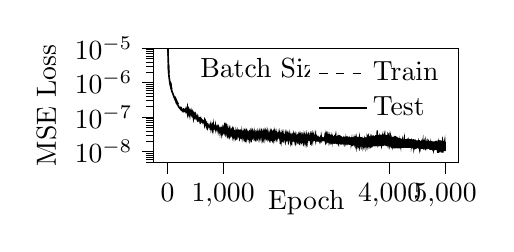
\begin{tikzpicture}

\begin{axis}[
legend cell align={left},
legend style={draw=none},
log basis y={10},
tick align=outside,
tick pos=left,
title={Batch Size 2},
title style={at={(0.4,0.85)},anchor=north},
x grid style={white!69.0196078431373!black},
xlabel={Epoch},
x label style={yshift=13pt},
xmin=-249.95, xmax=5248.95,
xtick style={color=black},
xtick = {0,1000,4000,5000},
y grid style={white!69.0196078431373!black},
ylabel={MSE Loss},
ymin=4.90143384155618e-09, ymax=1e-5,
ymode=log,
ytick style={color=black},
width=.45\textwidth,
height=.25\textwidth
]
\addplot [semithick, black, dashed]
table {%
0 0.00261398348659895
1 0.000146684363119675
2 7.82634508095725e-05
3 3.37719028447054e-05
4 2.5150746102085e-05
5 2.14879413085001e-05
6 1.73131360368757e-05
7 1.25710438198219e-05
8 8.384994563432e-06
9 6.01536302192685e-06
10 5.04094846438363e-06
11 4.50247262365266e-06
12 4.07342948584244e-06
13 3.68863333453007e-06
14 3.33568109506999e-06
15 3.02494765912797e-06
16 2.7562514826851e-06
17 2.52888349787028e-06
18 2.34137056487427e-06
19 2.18880018897138e-06
20 2.06381847633885e-06
21 1.96098151437774e-06
22 1.87465510770934e-06
23 1.80052594150659e-06
24 1.73351173886616e-06
25 1.67263015383323e-06
26 1.61614738892268e-06
27 1.56198234465066e-06
28 1.50867286552803e-06
29 1.46046563780544e-06
30 1.41356673157844e-06
31 1.37106688897681e-06
32 1.33059727563989e-06
33 1.28919083652868e-06
34 1.25175892679241e-06
35 1.21776896658865e-06
36 1.18564458267567e-06
37 1.15591732029952e-06
38 1.12700339668681e-06
39 1.10075354224648e-06
40 1.07587387876951e-06
41 1.05260377831939e-06
42 1.0313208120829e-06
43 1.01144230139827e-06
44 9.92442267119031e-07
45 9.7406527741839e-07
46 9.57213383753874e-07
47 9.40670659906218e-07
48 9.25038841827153e-07
49 9.10250043492766e-07
50 8.96198767826206e-07
51 8.83881172112133e-07
52 8.71137165300517e-07
53 8.58803400506147e-07
54 8.4801414614688e-07
55 8.36522416101104e-07
56 8.25851773152308e-07
57 8.15359453404163e-07
58 8.05294669189216e-07
59 7.95505481549164e-07
60 7.86104835461821e-07
61 7.76836224471111e-07
62 7.67232828448705e-07
63 7.40208569903089e-07
64 7.24697941538288e-07
65 7.12473284208315e-07
66 6.98334301669767e-07
67 6.8646508113801e-07
68 6.76835167410239e-07
69 6.67913647898644e-07
70 6.59476819643956e-07
71 6.51745536447201e-07
72 6.44344590145174e-07
73 6.37315424147467e-07
74 6.29807009134176e-07
75 6.23752871640626e-07
76 6.17110982172875e-07
77 6.10710473006648e-07
78 6.04971023602019e-07
79 5.99273899850594e-07
80 5.93674280890077e-07
81 5.88465108357639e-07
82 5.83262429605824e-07
83 5.78088403622168e-07
84 5.73076810137074e-07
85 5.68146300770955e-07
86 5.63457285606361e-07
87 5.59085755743816e-07
88 5.54764195544344e-07
89 5.50326957575287e-07
90 5.46110211153916e-07
91 5.41905436579171e-07
92 5.38032570275071e-07
93 5.33861362991495e-07
94 5.29962581785171e-07
95 5.25934999759059e-07
96 5.21953731732694e-07
97 5.17996030810153e-07
98 5.13999557568923e-07
99 5.10104440494707e-07
100 5.06136233847876e-07
101 5.02081006532151e-07
102 4.98216791648076e-07
103 4.94461015678738e-07
104 4.90604048617449e-07
105 4.86462815026734e-07
106 4.82587882216556e-07
107 4.78588768475063e-07
108 4.74869900535246e-07
109 4.7077929747541e-07
110 4.66663813166512e-07
111 4.62867599476446e-07
112 4.58659658813865e-07
113 4.54709814113663e-07
114 4.50870674558068e-07
115 4.46929221819659e-07
116 4.42388200826649e-07
117 4.38506839680386e-07
118 4.34678859113191e-07
119 4.3089226689208e-07
120 4.27085763439194e-07
121 4.23271578807061e-07
122 4.19777154811563e-07
123 4.15960641148239e-07
124 4.12074457444511e-07
125 4.08489014579239e-07
126 4.04658556217186e-07
127 4.00951681431394e-07
128 3.9733187562252e-07
129 3.93702260550022e-07
130 3.90062106880862e-07
131 3.86685338110482e-07
132 3.83489258807046e-07
133 3.79915736270497e-07
134 3.76464143924338e-07
135 3.73031685953151e-07
136 3.69614877314461e-07
137 3.66566005281399e-07
138 3.63254276162017e-07
139 3.59711858066269e-07
140 3.56280412384891e-07
141 3.52569088435395e-07
142 3.49126307100711e-07
143 3.45766744868303e-07
144 3.42371599904911e-07
145 3.39262808538354e-07
146 3.36348832967737e-07
147 3.33401700036262e-07
148 3.30368856395147e-07
149 3.2688863233421e-07
150 3.24198848596247e-07
151 3.21372436439926e-07
152 3.17807970312778e-07
153 3.15233077704757e-07
154 3.12444794476452e-07
155 3.10027523902079e-07
156 3.07321188873999e-07
157 3.04717508505359e-07
158 3.02148876103026e-07
159 2.99573802886144e-07
160 2.96987011524585e-07
161 2.94648659848296e-07
162 2.92419047800419e-07
163 2.90140671955541e-07
164 2.88099955823906e-07
165 2.8558504167453e-07
166 2.83444139733025e-07
167 2.8141647362645e-07
168 2.79245677041295e-07
169 2.77200937237154e-07
170 2.75588299680773e-07
171 2.73590638562027e-07
172 2.71654279449418e-07
173 2.69519297966259e-07
174 2.67458664513498e-07
175 2.65497534967629e-07
176 2.63673217523852e-07
177 2.61948017285185e-07
178 2.60005301479183e-07
179 2.58152771367648e-07
180 2.56357327418133e-07
181 2.54637377330891e-07
182 2.5292912211583e-07
183 2.51359738450141e-07
184 2.49551562201411e-07
185 2.48045789688955e-07
186 2.46444842606497e-07
187 2.4465752219438e-07
188 2.43001887576533e-07
189 2.41387644265956e-07
190 2.39743852080032e-07
191 2.38591042211134e-07
192 2.36896491812466e-07
193 2.35331076664291e-07
194 2.33869138022147e-07
195 2.32390313131603e-07
196 2.30942950676827e-07
197 2.29478455254561e-07
198 2.28119508614011e-07
199 2.26882294488195e-07
200 2.25635528665613e-07
201 2.24384542468314e-07
202 2.23268744437011e-07
203 2.21910245763457e-07
204 2.20867471478314e-07
205 2.19511795347405e-07
206 2.18217545115529e-07
207 2.17078903803181e-07
208 2.15910442586509e-07
209 2.14819290250023e-07
210 2.1386440760951e-07
211 2.12621667512458e-07
212 2.11595954674237e-07
213 2.10598725390199e-07
214 2.09534008213996e-07
215 2.08534801116933e-07
216 2.07571893242164e-07
217 2.06601709264564e-07
218 2.05631415472141e-07
219 2.04732785008765e-07
220 2.03928731128844e-07
221 2.02986788394366e-07
222 2.02125836123557e-07
223 2.01693005556169e-07
224 2.00247696379385e-07
225 1.99351367456746e-07
226 1.9847183270949e-07
227 1.97567987980651e-07
228 1.96726100124334e-07
229 1.95874223668291e-07
230 1.95032362352077e-07
231 1.9429453191222e-07
232 1.93577463155847e-07
233 1.92833159978534e-07
234 1.91930465522017e-07
235 1.91151176648585e-07
236 1.90727425620985e-07
237 1.89940357579133e-07
238 1.89282947241409e-07
239 1.88559956265433e-07
240 1.87832262899867e-07
241 1.87312221969105e-07
242 1.8638003640481e-07
243 1.85629820950606e-07
244 1.84861143206927e-07
245 1.84173773354779e-07
246 1.8346385132828e-07
247 1.82691622820474e-07
248 1.81981703223588e-07
249 1.81241538350196e-07
250 1.80819522359599e-07
251 1.80233316547929e-07
252 1.79373761339141e-07
253 1.78795408649846e-07
254 1.78261502097099e-07
255 1.77732386884122e-07
256 1.77024827346939e-07
257 1.76212229890949e-07
258 1.75559959624039e-07
259 1.75028014774092e-07
260 1.74455442444987e-07
261 1.73865569054188e-07
262 1.73293729991419e-07
263 1.72699000502652e-07
264 1.72175157529209e-07
265 1.71600795157545e-07
266 1.71060159445346e-07
267 1.70516953865052e-07
268 1.69965971575703e-07
269 1.69306111652556e-07
270 1.68603019955915e-07
271 1.68096036264442e-07
272 1.67533045300372e-07
273 1.67098511944852e-07
274 1.66452356481939e-07
275 1.6594090199118e-07
276 1.65430003029599e-07
277 1.6504094741765e-07
278 1.64535466716353e-07
279 1.64067817844948e-07
280 1.63518295869691e-07
281 1.63008348729843e-07
282 1.62516949801628e-07
283 1.62122773014195e-07
284 1.61727112577337e-07
285 1.61419068025026e-07
286 1.60981843060126e-07
287 1.60612840249152e-07
288 1.60113057938505e-07
289 1.59996616506453e-07
290 1.59500434703475e-07
291 1.59041253554371e-07
292 1.58633176553291e-07
293 1.58230017347494e-07
294 1.57726207859366e-07
295 1.57391601654178e-07
296 1.56932869004311e-07
297 1.56524124702795e-07
298 1.56090241693274e-07
299 1.55728700207858e-07
300 1.55397476291563e-07
301 1.54913462214301e-07
302 1.54460410595414e-07
303 1.54037259622264e-07
304 1.53807496733549e-07
305 1.53307295429617e-07
306 1.52889717186522e-07
307 1.52815606427659e-07
308 1.5255875534792e-07
309 1.51992299653791e-07
310 1.51631543023223e-07
311 1.51434879765988e-07
312 1.50798544854336e-07
313 1.50500502398065e-07
314 1.50309462715548e-07
315 1.5012875835807e-07
316 1.49606689905601e-07
317 1.49262755533508e-07
318 1.489406507591e-07
319 1.48563328749907e-07
320 1.48307872039899e-07
321 1.47996224146629e-07
322 1.47477975280585e-07
323 1.46864158302451e-07
324 1.46399182789247e-07
325 1.4600326030334e-07
326 1.45447961132694e-07
327 1.45286996641181e-07
328 1.45124027577159e-07
329 1.4457256800382e-07
330 1.44243595714633e-07
331 1.43893380800231e-07
332 1.43401146519118e-07
333 1.43232647254354e-07
334 1.42721284159375e-07
335 1.42463075213817e-07
336 1.42195513040511e-07
337 1.41774924736993e-07
338 1.41613115455463e-07
339 1.41290982773601e-07
340 1.40814341321294e-07
341 1.40588078612947e-07
342 1.40190531043416e-07
343 1.39982248199333e-07
344 1.39655671995254e-07
345 1.39315308924859e-07
346 1.39008234261606e-07
347 1.38621841989428e-07
348 1.38385781822015e-07
349 1.38106749037359e-07
350 1.37768745258837e-07
351 1.37302368972358e-07
352 1.37273293095319e-07
353 1.36685038603535e-07
354 1.36805641671289e-07
355 1.36218938038724e-07
356 1.36174170560555e-07
357 1.35144350333238e-07
358 1.35377791940172e-07
359 1.3519789696903e-07
360 1.34321391878522e-07
361 1.34628653254643e-07
362 1.34382502061214e-07
363 1.33540979393221e-07
364 1.33748807011447e-07
365 1.33484170640186e-07
366 1.32627974005484e-07
367 1.3297263567158e-07
368 1.32693508702708e-07
369 1.32514474537659e-07
370 1.32011076459548e-07
371 1.31861206790651e-07
372 1.31521757749109e-07
373 1.31331652518663e-07
374 1.31312317972254e-07
375 1.30603197236123e-07
376 1.30561156867826e-07
377 1.29773564399915e-07
378 1.30057639510683e-07
379 1.29861310177226e-07
380 1.29112238212326e-07
381 1.29198381696227e-07
382 1.28842748736258e-07
383 1.2872677043152e-07
384 1.2815145879741e-07
385 1.28243387647053e-07
386 1.28023895214824e-07
387 1.27487541142557e-07
388 1.27568656234978e-07
389 1.27031404781208e-07
390 1.27159839126145e-07
391 1.26598800443301e-07
392 1.26791784661684e-07
393 1.26477510927092e-07
394 1.26444590979657e-07
395 1.26158001562349e-07
396 1.25962107867528e-07
397 1.25775401044637e-07
398 1.25593913733013e-07
399 1.24813759142306e-07
400 1.25107088592591e-07
401 1.24789898830358e-07
402 1.24521163066271e-07
403 1.24255962218545e-07
404 1.24277898207348e-07
405 1.23580057124872e-07
406 1.23692217324445e-07
407 1.23466668605632e-07
408 1.23292362624872e-07
409 1.23125864866624e-07
410 1.22844255137977e-07
411 1.22260624106474e-07
412 1.22632293348746e-07
413 1.22149892797907e-07
414 1.21888570189244e-07
415 1.2183269884436e-07
416 1.21501794058565e-07
417 1.21598056354921e-07
418 1.21115364892788e-07
419 1.20845609222542e-07
420 1.20702182457633e-07
421 1.20670180585147e-07
422 1.20313101976244e-07
423 1.20242447746888e-07
424 1.19796707906294e-07
425 1.19679437805553e-07
426 1.19502443590935e-07
427 1.19306255657259e-07
428 1.19001857039169e-07
429 1.18975247541897e-07
430 1.18751168056708e-07
431 1.18668970422453e-07
432 1.18519750465174e-07
433 1.18310549850564e-07
434 1.18205436012264e-07
435 1.18052298470728e-07
436 1.17879357376394e-07
437 1.17379495784053e-07
438 1.17300958525135e-07
439 1.17437472770154e-07
440 1.17254779579357e-07
441 1.16698817170358e-07
442 1.1665886642831e-07
443 1.16422076178457e-07
444 1.16437312810413e-07
445 1.16211605543537e-07
446 1.15907504869339e-07
447 1.15631951317585e-07
448 1.15533178603799e-07
449 1.1553922251073e-07
450 1.15184505566468e-07
451 1.15018143974188e-07
452 1.15032055581388e-07
453 1.14700197587414e-07
454 1.14470164584324e-07
455 1.14392085056592e-07
456 1.14392627027948e-07
457 1.13851511679419e-07
458 1.13809522381825e-07
459 1.13363633469143e-07
460 1.13507051060058e-07
461 1.12955144015325e-07
462 1.12687809270984e-07
463 1.12958656940165e-07
464 1.12561146591084e-07
465 1.1211510408593e-07
466 1.11795333277431e-07
467 1.11874699544767e-07
468 1.11499599053211e-07
469 1.11183911756685e-07
470 1.1097315462405e-07
471 1.10746568335651e-07
472 1.10528108287378e-07
473 1.10256356484095e-07
474 1.10099632397498e-07
475 1.09766951710499e-07
476 1.09138375835371e-07
477 1.08834864133156e-07
478 1.0881889858938e-07
479 1.08393336007095e-07
480 1.08144232992657e-07
481 1.0793406884968e-07
482 1.07731355728502e-07
483 1.07404242227993e-07
484 1.07224436205255e-07
485 1.06623043470755e-07
486 1.06600979004057e-07
487 1.06223428439911e-07
488 1.06042661533579e-07
489 1.05791827745172e-07
490 1.05572618482874e-07
491 1.05332027782401e-07
492 1.05210153051427e-07
493 1.04844322206032e-07
494 1.04628191569089e-07
495 1.04377984629922e-07
496 1.04216347538877e-07
497 1.03955194479699e-07
498 1.03688604859542e-07
499 1.03510769820403e-07
500 1.03342628648528e-07
501 1.03084363703987e-07
502 1.0284133121341e-07
503 1.02668651758897e-07
504 1.02572349458985e-07
505 1.02124076692522e-07
506 1.01995372278507e-07
507 1.01731550677941e-07
508 1.01490412855565e-07
509 1.01381675744916e-07
510 1.01240593376462e-07
511 1.00909068223354e-07
512 1.00669337769643e-07
513 1.00404250107822e-07
514 1.00423404139294e-07
515 1.00214220461581e-07
516 9.99527497607122e-08
517 9.97062718719466e-08
518 9.94624701242675e-08
519 9.93852768302883e-08
520 9.90874772937023e-08
521 9.88455424544288e-08
522 9.86786483039293e-08
523 9.85174300247582e-08
524 9.83541504726571e-08
525 9.82658134411896e-08
526 9.78364765480411e-08
527 9.77660970995498e-08
528 9.7614606940466e-08
529 9.7288654843819e-08
530 9.69792118370449e-08
531 9.69268959594149e-08
532 9.67892044398955e-08
533 9.64910404850361e-08
534 9.62170009874974e-08
535 9.62202412035929e-08
536 9.58558749346583e-08
537 9.56776447187391e-08
538 9.5498134587757e-08
539 9.53894120798715e-08
540 9.50934551380289e-08
541 9.48801197169224e-08
542 9.46125329708281e-08
543 9.44436887060363e-08
544 9.4335708752169e-08
545 9.40767704953327e-08
546 9.38061104351906e-08
547 9.36843962597855e-08
548 9.34865146009489e-08
549 9.32645453668446e-08
550 9.30323500869523e-08
551 9.2910364995813e-08
552 9.24915208440069e-08
553 9.26237489684567e-08
554 9.20383658806756e-08
555 9.20737594465315e-08
556 9.1773045729715e-08
557 9.15990957992552e-08
558 9.16372675546784e-08
559 9.13390870608266e-08
560 9.12179028298432e-08
561 9.10503901381254e-08
562 9.07964728142918e-08
563 9.05843692435848e-08
564 9.03890795960205e-08
565 9.00719094163449e-08
566 8.99008989017069e-08
567 8.98419131223349e-08
568 8.94903660499935e-08
569 8.92771059846087e-08
570 8.92133772965043e-08
571 8.92505096738994e-08
572 8.88596866948088e-08
573 8.88809712964456e-08
574 8.85358828333072e-08
575 8.83346679561026e-08
576 8.84105503005106e-08
577 8.8131889763865e-08
578 8.80912545679902e-08
579 8.76220811723005e-08
580 8.76374261120638e-08
581 8.73306817090747e-08
582 8.69455808030217e-08
583 8.70990354120416e-08
584 8.65921273616177e-08
585 8.64360111918483e-08
586 8.64471381185616e-08
587 8.61044444553372e-08
588 8.59900289835735e-08
589 8.59733905260729e-08
590 8.56495371353017e-08
591 8.5448452592729e-08
592 8.52556495878343e-08
593 8.50720472700406e-08
594 8.48990268551564e-08
595 8.46750809213592e-08
596 8.45080046549818e-08
597 8.42445121276292e-08
598 8.40143372828894e-08
599 8.37218631160042e-08
600 8.35349402392716e-08
601 8.31654908488577e-08
602 8.30242949245719e-08
603 8.2982439593593e-08
604 8.2921621885168e-08
605 8.26500533532837e-08
606 8.25823081787025e-08
607 8.2389301115926e-08
608 8.22421491531999e-08
609 8.19840703343289e-08
610 8.1801761944611e-08
611 8.18592255097395e-08
612 8.16676565214003e-08
613 8.16171640491969e-08
614 8.13247282057672e-08
615 8.10373738009407e-08
616 8.08642084723088e-08
617 8.06555648807938e-08
618 8.039214622102e-08
619 8.02460349925704e-08
620 8.00810798282647e-08
621 7.99409526959227e-08
622 7.97110490066144e-08
623 7.94116076875406e-08
624 7.92543457824868e-08
625 7.90482818721072e-08
626 7.87830216444352e-08
627 7.86491988641336e-08
628 7.84446622161816e-08
629 7.827243654146e-08
630 7.81483883874889e-08
631 7.79432979882699e-08
632 7.77564276402964e-08
633 7.75270853509147e-08
634 7.74125279346949e-08
635 7.70996542881486e-08
636 7.70233436728773e-08
637 7.66381009270622e-08
638 7.64740521639329e-08
639 7.66816242462332e-08
640 7.64246416755654e-08
641 7.61894967465926e-08
642 7.59976832137577e-08
643 7.56666841013054e-08
644 7.54723867576468e-08
645 7.54306852314146e-08
646 7.53268538478125e-08
647 7.51730338366396e-08
648 7.47495809915177e-08
649 7.48541830168925e-08
650 7.43791588843079e-08
651 7.42978026984087e-08
652 7.42460074155682e-08
653 7.40438198457705e-08
654 7.3634554738522e-08
655 7.37113431152903e-08
656 7.34467651670734e-08
657 7.33724932918678e-08
658 7.31816905603644e-08
659 7.31439444945359e-08
660 7.28667297711372e-08
661 7.26887656533615e-08
662 7.25385389976907e-08
663 7.24498825926956e-08
664 7.22832119443018e-08
665 7.21822083353807e-08
666 7.19495448092688e-08
667 7.18707898982318e-08
668 7.16480042597389e-08
669 7.14073806823423e-08
670 7.13205865152666e-08
671 7.10196900129967e-08
672 7.09722795270151e-08
673 7.07187652627672e-08
674 7.06024032132158e-08
675 7.05165593821722e-08
676 7.03380461603009e-08
677 7.03425385415457e-08
678 7.00737257445239e-08
679 6.99320477606236e-08
680 6.97025158427067e-08
681 6.95539946653501e-08
682 6.93178849876519e-08
683 6.94211070342288e-08
684 6.90671745279259e-08
685 6.8847339870004e-08
686 6.89086112218851e-08
687 6.87327516597502e-08
688 6.84967959185823e-08
689 6.84914813144921e-08
690 6.84173265950161e-08
691 6.81482263986677e-08
692 6.79657498626751e-08
693 6.76911481836129e-08
694 6.78754415739391e-08
695 6.76873341790563e-08
696 6.7420077696112e-08
697 6.73318192355721e-08
698 6.71849346519648e-08
699 6.70631731659599e-08
700 6.6936109860527e-08
701 6.67347293343834e-08
702 6.66230708357141e-08
703 6.67056503975694e-08
704 6.66208884274599e-08
705 6.6402336841076e-08
706 6.637572022683e-08
707 6.60298795550629e-08
708 6.58703416722695e-08
709 6.59932807797192e-08
710 6.57574264092409e-08
711 6.5755870203299e-08
712 6.55362282209193e-08
713 6.54728074114264e-08
714 6.5351697348004e-08
715 6.53087951680842e-08
716 6.51708659051842e-08
717 6.50125667877033e-08
718 6.49798564733572e-08
719 6.47724273014072e-08
720 6.47707329970437e-08
721 6.45535312721046e-08
722 6.44558372296933e-08
723 6.43093136186712e-08
724 6.406546154758e-08
725 6.40719362525743e-08
726 6.45583160179264e-08
727 6.38616268305858e-08
728 6.39997100977396e-08
729 6.38944717001877e-08
730 6.37970664736365e-08
731 6.36738414186988e-08
732 6.35405101436781e-08
733 6.3468621691154e-08
734 6.31237134999241e-08
735 6.32146194542438e-08
736 6.31069264531714e-08
737 6.30518270504643e-08
738 6.29606186937082e-08
739 6.26848402600633e-08
740 6.28600875853813e-08
741 6.26476349310234e-08
742 6.24892591627457e-08
743 6.24455489549591e-08
744 6.23294498194316e-08
745 6.2253770162779e-08
746 6.21718271596183e-08
747 6.20670583866279e-08
748 6.18798210956228e-08
749 6.188538615437e-08
750 6.18037680910621e-08
751 6.16810066836893e-08
752 6.15384937397989e-08
753 6.14532277937174e-08
754 6.1445070853372e-08
755 6.13365998902715e-08
756 6.12798440569051e-08
757 6.13104954930721e-08
758 6.12681508648238e-08
759 6.10669092498961e-08
760 6.10586326349472e-08
761 6.09786342657959e-08
762 6.08765920058207e-08
763 6.07757833117617e-08
764 6.07843563827926e-08
765 6.05380540213973e-08
766 6.04225618350274e-08
767 6.03992417815835e-08
768 6.03464287243227e-08
769 6.01462231776262e-08
770 6.00604040950081e-08
771 6.00231084527669e-08
772 5.99093010943408e-08
773 5.98377934263317e-08
774 5.96081898500689e-08
775 5.95742457141224e-08
776 5.96780586127332e-08
777 5.93245081615956e-08
778 5.91501711765252e-08
779 5.92791223117395e-08
780 5.91412333191821e-08
781 5.90747720404794e-08
782 5.89476858179339e-08
783 5.88208731741036e-08
784 5.88255402458326e-08
785 5.8786889870488e-08
786 5.86065183543205e-08
787 5.86318991023793e-08
788 5.8584062483602e-08
789 5.84684124078638e-08
790 5.85145645294327e-08
791 5.82407579362565e-08
792 5.82223076095456e-08
793 5.79912457159271e-08
794 5.8108856008543e-08
795 5.79709602686052e-08
796 5.78531142740868e-08
797 5.78370420644125e-08
798 5.76913316553407e-08
799 5.76839951780261e-08
800 5.75831435745133e-08
801 5.75909274685982e-08
802 5.74083612785437e-08
803 5.74391697699683e-08
804 5.72027329296398e-08
805 5.73407223503075e-08
806 5.72023227312091e-08
807 5.70735137997991e-08
808 5.70729130350278e-08
809 5.69626252675537e-08
810 5.6882644279832e-08
811 5.68058462963039e-08
812 5.66683241300936e-08
813 5.66744659303842e-08
814 5.65901798542656e-08
815 5.6436309426422e-08
816 5.65831056307253e-08
817 5.63878848396371e-08
818 5.62771926944095e-08
819 5.62657206842898e-08
820 5.62157826032861e-08
821 5.61009023639647e-08
822 5.60516779550824e-08
823 5.59690822986569e-08
824 5.61079724488156e-08
825 5.58611277436949e-08
826 5.57958161638838e-08
827 5.57157521758889e-08
828 5.56878466763111e-08
829 5.57414290146552e-08
830 5.54114399603511e-08
831 5.54050776053749e-08
832 5.54322031087739e-08
833 5.54243826426104e-08
834 5.53643694637396e-08
835 5.51954801198962e-08
836 5.53016565781883e-08
837 5.52197657462949e-08
838 5.50475004045259e-08
839 5.50929451459403e-08
840 5.49398851192873e-08
841 5.50032194527317e-08
842 5.49059920349482e-08
843 5.48543149434533e-08
844 5.47220845609209e-08
845 5.45919308593268e-08
846 5.46621458888952e-08
847 5.45036415513511e-08
848 5.44871118437484e-08
849 5.44909918462899e-08
850 5.44362895656958e-08
851 5.42284673225035e-08
852 5.43319143780918e-08
853 5.42738582536284e-08
854 5.39490024304978e-08
855 5.41623808413272e-08
856 5.38711755492249e-08
857 5.38292376828231e-08
858 5.38144721166089e-08
859 5.40801493253973e-08
860 5.35556771573686e-08
861 5.34009007191472e-08
862 5.36913170899878e-08
863 5.35750088621612e-08
864 5.34702983183699e-08
865 5.31324628701979e-08
866 5.32663798854527e-08
867 5.34713005498899e-08
868 5.3268240315818e-08
869 5.3106281430626e-08
870 5.30999553991496e-08
871 5.30073745623749e-08
872 5.3024831385029e-08
873 5.29475644116539e-08
874 5.29035295295799e-08
875 5.27633898719237e-08
876 5.27644872644339e-08
877 5.26363374481198e-08
878 5.21344579949012e-08
879 5.26222953115552e-08
880 5.25046283263997e-08
881 5.25887310142137e-08
882 5.23786171260365e-08
883 5.22556745392588e-08
884 5.22890715103364e-08
885 5.22051752521735e-08
886 5.22562960395545e-08
887 5.21403642420593e-08
888 5.21259177299616e-08
889 5.23303570957312e-08
890 5.21940686630806e-08
891 5.20369648042696e-08
892 5.18643744533698e-08
893 5.1959078596342e-08
894 5.1800517703815e-08
895 5.17839124822839e-08
896 5.1749980221838e-08
897 5.20235737372365e-08
898 5.14930678036096e-08
899 5.13947631269884e-08
900 5.14576784906851e-08
901 5.15045462358144e-08
902 5.14380473438658e-08
903 5.14084751558341e-08
904 5.13051172055246e-08
905 5.13162940889433e-08
906 5.12426185311776e-08
907 5.11894807858626e-08
908 5.12040236309019e-08
909 5.11771593126875e-08
910 5.1391161834613e-08
911 5.09132827229974e-08
912 5.07956156252654e-08
913 5.07086769411247e-08
914 5.07240060290126e-08
915 5.05156226283665e-08
916 5.09034994145008e-08
917 5.10812179872477e-08
918 5.09299017443787e-08
919 5.06071179470213e-08
920 5.06153786566932e-08
921 5.08228125277732e-08
922 5.07701664046456e-08
923 5.04631669587807e-08
924 5.04625080791632e-08
925 5.03999359618978e-08
926 5.03120141140956e-08
927 5.02950299255955e-08
928 5.02036412520779e-08
929 5.05533185670704e-08
930 5.03805240215094e-08
931 5.03134604930011e-08
932 5.03399029133655e-08
933 5.02495765224431e-08
934 5.02485439819456e-08
935 5.01097002670869e-08
936 4.98450323295208e-08
937 5.00081839931443e-08
938 5.02201354417586e-08
939 5.00173292057315e-08
940 4.99454150872936e-08
941 4.98917330522541e-08
942 4.97869760859304e-08
943 4.96477238839388e-08
944 4.96061485512067e-08
945 4.96272340385628e-08
946 4.96270244700892e-08
947 4.96611786039436e-08
948 4.93043708666985e-08
949 4.93675331766363e-08
950 4.94701070694603e-08
951 4.95901512781449e-08
952 4.95660200040549e-08
953 4.93224323655506e-08
954 4.91889253581013e-08
955 4.92657079411152e-08
956 4.93090457755474e-08
957 4.90304114769136e-08
958 4.86113878614414e-08
959 4.87386970814407e-08
960 4.86080396257527e-08
961 4.91473815086851e-08
962 4.82496446461145e-08
963 4.8349681513904e-08
964 4.83994517888053e-08
965 4.84674849848266e-08
966 4.89019669674406e-08
967 4.87339815461452e-08
968 4.8887384868801e-08
969 4.86750621041532e-08
970 4.87458362598003e-08
971 4.87206623641101e-08
972 4.85998083747385e-08
973 4.86616961933861e-08
974 4.85624361134529e-08
975 4.85805682470253e-08
976 4.85125720613433e-08
977 4.82887160206391e-08
978 4.84719224294605e-08
979 4.83484899962972e-08
980 4.82735046126725e-08
981 4.84206677583976e-08
982 4.82095535099814e-08
983 4.81738937898046e-08
984 4.81529513432499e-08
985 4.80463511752238e-08
986 4.8008118166909e-08
987 4.78388747605085e-08
988 4.79545476203547e-08
989 4.77904276480756e-08
990 4.76947455610444e-08
991 4.7953770904885e-08
992 4.75322841403392e-08
993 4.7785734386907e-08
994 4.75348239130091e-08
995 4.7667171884147e-08
996 4.74739370615596e-08
997 4.75618149212709e-08
998 4.75811124144854e-08
999 4.74248252290144e-08
1000 4.76309443844802e-08
1001 4.72376396284391e-08
1002 4.71671802128038e-08
1003 4.74440110288521e-08
1004 4.69942068811458e-08
1005 4.71157604259309e-08
1006 4.69819341240574e-08
1007 4.69522687752133e-08
1008 4.68813971180038e-08
1009 4.66572676727783e-08
1010 4.68712826183215e-08
1011 4.65230975445485e-08
1012 4.6986280031025e-08
1013 4.65285257113535e-08
1014 4.65172853401641e-08
1015 4.69000739997116e-08
1016 4.59802069521786e-08
1017 4.61438803179282e-08
1018 4.61487103370906e-08
1019 4.60385496252047e-08
1020 4.60279651077755e-08
1021 4.5991702721071e-08
1022 4.6049907213741e-08
1023 4.58232247232404e-08
1024 4.575472711843e-08
1025 4.57867423995784e-08
1026 4.57194202890809e-08
1027 4.5735625373744e-08
1028 4.56614160241897e-08
1029 4.57159697072051e-08
1030 4.55817242379086e-08
1031 4.55687318516862e-08
1032 4.55431716767651e-08
1033 4.54868766998073e-08
1034 4.54809728112071e-08
1035 4.53985480052266e-08
1036 4.5422408025686e-08
1037 4.52892244754421e-08
1038 4.52831030046119e-08
1039 4.53999871000699e-08
1040 4.54181504337958e-08
1041 4.52862972734613e-08
1042 4.51580050345179e-08
1043 4.51480138310423e-08
1044 4.51643003261393e-08
1045 4.51240597721392e-08
1046 4.49955824772252e-08
1047 4.50499606158838e-08
1048 4.50189186058103e-08
1049 4.50657565729817e-08
1050 4.4959013388024e-08
1051 4.48627814274016e-08
1052 4.48606086906889e-08
1053 4.4802549736378e-08
1054 4.48229560718882e-08
1055 4.48897614062638e-08
1056 4.47645272669828e-08
1057 4.46646057877254e-08
1058 4.47493429872603e-08
1059 4.46290876262023e-08
1060 4.47393384138683e-08
1061 4.44872028639853e-08
1062 4.46542057774835e-08
1063 4.44682002784802e-08
1064 4.45064564659758e-08
1065 4.45753047110253e-08
1066 4.4414909836088e-08
1067 4.44585654978957e-08
1068 4.43124520668192e-08
1069 4.43833488869561e-08
1070 4.4300507340167e-08
1071 4.42940364882016e-08
1072 4.42912890031288e-08
1073 4.43040135522099e-08
1074 4.42048048830967e-08
1075 4.416254044598e-08
1076 4.41335653407759e-08
1077 4.40365813249022e-08
1078 4.41081502742802e-08
1079 4.40969820470483e-08
1080 4.3948786994652e-08
1081 4.41720446373584e-08
1082 4.39464986777271e-08
1083 4.40942140758627e-08
1084 4.37837767735538e-08
1085 4.39278263835718e-08
1086 4.37930967392974e-08
1087 4.37182112345003e-08
1088 4.37573598288665e-08
1089 4.37867421974048e-08
1090 4.36447713969557e-08
1091 4.38515382742977e-08
1092 4.37362916652084e-08
1093 4.36174015362445e-08
1094 4.3778218633217e-08
1095 4.35680120209891e-08
1096 4.35805192225414e-08
1097 4.36738350335086e-08
1098 4.36676859579821e-08
1099 4.35005779383379e-08
1100 4.35071349083049e-08
1101 4.35172271734396e-08
1102 4.34009853089168e-08
1103 4.33678863978049e-08
1104 4.33504221901138e-08
1105 4.32441569210851e-08
1106 4.3280685350644e-08
1107 4.34523939446541e-08
1108 4.32948200780325e-08
1109 4.31160244203088e-08
1110 4.31606878995017e-08
1111 4.31132841002824e-08
1112 4.31126667642112e-08
1113 4.30161841746823e-08
1114 4.31351706885463e-08
1115 4.30137107217399e-08
1116 4.30419452301378e-08
1117 4.28521687167449e-08
1118 4.29494802055563e-08
1119 4.2983084970083e-08
1120 4.28279311986968e-08
1121 4.29285861436868e-08
1122 4.28456561525348e-08
1123 4.29562623107116e-08
1124 4.28213921451759e-08
1125 4.27720357785155e-08
1126 4.27197061031448e-08
1127 4.27676665794574e-08
1128 4.27508851308933e-08
1129 4.2682300908925e-08
1130 4.26003897978089e-08
1131 4.24758110147416e-08
1132 4.25463953803162e-08
1133 4.25152052525024e-08
1134 4.25598208884104e-08
1135 4.239308792503e-08
1136 4.2449155177704e-08
1137 4.24381763784454e-08
1138 4.24335556179489e-08
1139 4.23089017043132e-08
1140 4.23211221574071e-08
1141 4.22933782630586e-08
1142 4.23067300873714e-08
1143 4.23677056163863e-08
1144 4.23486314717891e-08
1145 4.19986635529779e-08
1146 4.20469467001805e-08
1147 4.22094996923028e-08
1148 4.20193057089624e-08
1149 4.21166019328179e-08
1150 4.21501204259656e-08
1151 4.19883999723814e-08
1152 4.20073089106854e-08
1153 4.18943582077835e-08
1154 4.19936113004726e-08
1155 4.20366788216886e-08
1156 4.20818990342631e-08
1157 4.18583599697264e-08
1158 4.17444217319929e-08
1159 4.17618667362674e-08
1160 4.17829855202667e-08
1161 4.17799846383904e-08
1162 4.16705735562517e-08
1163 4.18948547789011e-08
1164 4.16620335019213e-08
1165 4.17125577941713e-08
1166 4.15728996195353e-08
1167 4.16248975123046e-08
1168 4.17766256601282e-08
1169 4.14573240685168e-08
1170 4.15731547034337e-08
1171 4.14832258551212e-08
1172 4.14894388031661e-08
1173 4.17455580651316e-08
1174 4.15013680700738e-08
1175 4.15968621256257e-08
1176 4.13717257054524e-08
1177 4.15543938007135e-08
1178 4.12514978142542e-08
1179 4.14077720277683e-08
1180 4.15308862883323e-08
1181 4.13152643243264e-08
1182 4.13804941682416e-08
1183 4.13969383722401e-08
1184 4.13074685233217e-08
1185 4.14006716444315e-08
1186 4.12031826499959e-08
1187 4.13484403469777e-08
1188 4.11279918449137e-08
1189 4.1116992403778e-08
1190 4.10200866945987e-08
1191 4.10916682780371e-08
1192 4.10232857664949e-08
1193 4.11754650986307e-08
1194 4.08613160786109e-08
1195 4.10294067033634e-08
1196 4.11262635822141e-08
1197 4.09699648660222e-08
1198 4.09178326050697e-08
1199 4.08179365538608e-08
1200 4.08433911486261e-08
1201 4.07925646619955e-08
1202 4.0843865591389e-08
1203 4.08273227012201e-08
1204 4.08248592192462e-08
1205 4.09464814088434e-08
1206 4.07076831734909e-08
1207 4.06216350464228e-08
1208 4.05717194499888e-08
1209 4.07536141571185e-08
1210 4.06037834261297e-08
1211 4.05800763356723e-08
1212 4.05475472338157e-08
1213 4.05940800142779e-08
1214 4.07310513145798e-08
1215 4.0481364380951e-08
1216 4.05854570876274e-08
1217 4.0419865971697e-08
1218 4.04724098932996e-08
1219 4.03760262344677e-08
1220 4.05545208236879e-08
1221 4.04062817561668e-08
1222 4.04085032262302e-08
1223 4.0206302078627e-08
1224 4.02853182185359e-08
1225 4.02691618917039e-08
1226 4.02556384009323e-08
1227 3.99654077228306e-08
1228 4.0084840536081e-08
1229 3.99519415278937e-08
1230 3.99425685834176e-08
1231 3.99511088683413e-08
1232 3.99962168105006e-08
1233 3.98757909992886e-08
1234 3.99903259502565e-08
1235 3.97727424241157e-08
1236 3.97362323014128e-08
1237 3.98615986861861e-08
1238 3.97920895919279e-08
1239 3.96503417985916e-08
1240 3.98500998187723e-08
1241 3.94888271154081e-08
1242 3.97363479529567e-08
1243 3.9670114947099e-08
1244 3.95152142287913e-08
1245 3.94588912658311e-08
1246 3.96170589693212e-08
1247 3.95713690846677e-08
1248 3.9653338033907e-08
1249 3.96299430795444e-08
1250 3.93851973877202e-08
1251 3.95682592178592e-08
1252 3.94245985052555e-08
1253 3.94186836629173e-08
1254 3.93995191990681e-08
1255 3.94417245035417e-08
1256 3.93175576240967e-08
1257 3.93010308639696e-08
1258 3.94500662774244e-08
1259 3.92660184653781e-08
1260 3.91611785369173e-08
1261 3.93277218297405e-08
1262 3.90468253679832e-08
1263 3.92391634491673e-08
1264 3.90210088450083e-08
1265 3.90619693654837e-08
1266 3.91635332250839e-08
1267 3.91998140386596e-08
1268 3.88992044481062e-08
1269 3.92167338549299e-08
1270 3.88048741853941e-08
1271 3.90122393857384e-08
1272 3.90509703188657e-08
1273 3.89146043306421e-08
1274 3.89563392785841e-08
1275 3.89260859701701e-08
1276 3.90563198613969e-08
1277 3.903581282938e-08
1278 3.87682184300187e-08
1279 3.90418795276903e-08
1280 3.88307571365099e-08
1281 3.88432197571675e-08
1282 3.88089232857825e-08
1283 3.88497545305011e-08
1284 3.8808237176613e-08
1285 3.86636885413849e-08
1286 3.8951220149408e-08
1287 3.87320291024285e-08
1288 3.86920816649039e-08
1289 3.8919329096998e-08
1290 3.86722198195133e-08
1291 3.86278853801714e-08
1292 3.88914554788622e-08
1293 3.8599475284451e-08
1294 3.8693181822369e-08
1295 3.85323008162963e-08
1296 3.85450245753982e-08
1297 3.8618123346601e-08
1298 3.86272235451401e-08
1299 3.85501028578594e-08
1300 3.85360730471018e-08
1301 3.84817750264665e-08
1302 3.83798020365811e-08
1303 3.84028968161143e-08
1304 3.83411669929168e-08
1305 3.86072583850039e-08
1306 3.83613074982914e-08
1307 3.8552181814977e-08
1308 3.82130065704755e-08
1309 3.80664171260592e-08
1310 3.84765729979919e-08
1311 3.81774920919509e-08
1312 3.82775483957487e-08
1313 3.83419538739216e-08
1314 3.82416022891574e-08
1315 3.81589909581037e-08
1316 3.84554827882466e-08
1317 3.81900211631758e-08
1318 3.80497460764073e-08
1319 3.80913908638036e-08
1320 3.79748055899243e-08
1321 3.82118173543611e-08
1322 3.8044942906712e-08
1323 3.7897786287433e-08
1324 3.80364340222261e-08
1325 3.80164513292258e-08
1326 3.80070932131105e-08
1327 3.77907139890721e-08
1328 3.79741725815008e-08
1329 3.7962045192963e-08
1330 3.78899051253767e-08
1331 3.78060559529936e-08
1332 3.78670913306345e-08
1333 3.78315917831662e-08
1334 3.80222686703902e-08
1335 3.77478427376343e-08
1336 3.76959864369364e-08
1337 3.76758144395861e-08
1338 3.78092513653727e-08
1339 3.77412872711314e-08
1340 3.76240642890879e-08
1341 3.77037665962865e-08
1342 3.75619689473861e-08
1343 3.77010441950931e-08
1344 3.77110146798088e-08
1345 3.75804105830491e-08
1346 3.76246193385943e-08
1347 3.75692676248818e-08
1348 3.74983338812807e-08
1349 3.74260324288445e-08
1350 3.73596034612955e-08
1351 3.74343606266425e-08
1352 3.74937736646319e-08
1353 3.75229895516749e-08
1354 3.71330517868751e-08
1355 3.74137304480215e-08
1356 3.7181566376332e-08
1357 3.72471152274567e-08
1358 3.74778136069676e-08
1359 3.72647145150395e-08
1360 3.72154928966473e-08
1361 3.7239597339922e-08
1362 3.72700734292408e-08
1363 3.74581570247168e-08
1364 3.7001714643492e-08
1365 3.71595026116833e-08
1366 3.72408672513203e-08
1367 3.7080263740441e-08
1368 3.72318790692883e-08
1369 3.70415177685657e-08
1370 3.72782474327149e-08
1371 3.70204627198611e-08
1372 3.70034276288567e-08
1373 3.71566659543299e-08
1374 3.69266780143596e-08
1375 3.71390608163713e-08
1376 3.69570218351489e-08
1377 3.6941323282691e-08
1378 3.6822000582748e-08
1379 3.6959429911998e-08
1380 3.68920858652144e-08
1381 3.701040906956e-08
1382 3.681259792776e-08
1383 3.66875012499102e-08
1384 3.6890900990294e-08
1385 3.68982291191755e-08
1386 3.69947587329777e-08
1387 3.70211979827673e-08
1388 3.68647417595125e-08
1389 3.6786965299962e-08
1390 3.69163455046229e-08
1391 3.6661925532866e-08
1392 3.68543216258121e-08
1393 3.68127328680412e-08
1394 3.68141683004253e-08
1395 3.68085077421254e-08
1396 3.67071528235008e-08
1397 3.68935591985031e-08
1398 3.66122590514939e-08
1399 3.66694211784147e-08
1400 3.65310263724661e-08
1401 3.66279319389262e-08
1402 3.64981576203016e-08
1403 3.64699415433267e-08
1404 3.67245235168845e-08
1405 3.65029932370975e-08
1406 3.66564263549751e-08
1407 3.66455188268722e-08
1408 3.64214779541294e-08
1409 3.65147219616446e-08
1410 3.67536794762535e-08
1411 3.66980817745333e-08
1412 3.63030791232788e-08
1413 3.66292846185612e-08
1414 3.64065608632891e-08
1415 3.63810815168786e-08
1416 3.65551502848893e-08
1417 3.63827365366665e-08
1418 3.68315672601427e-08
1419 3.6253791672769e-08
1420 3.65551811753462e-08
1421 3.63489426132846e-08
1422 3.64301096009711e-08
1423 3.63845785113504e-08
1424 3.63241670645609e-08
1425 3.62743841785806e-08
1426 3.64269679675733e-08
1427 3.62643482531011e-08
1428 3.64093605202953e-08
1429 3.65368469820715e-08
1430 3.64458330048834e-08
1431 3.61357457412947e-08
1432 3.62946508546957e-08
1433 3.61692249251089e-08
1434 3.63927227604033e-08
1435 3.62667733102562e-08
1436 3.6191466375235e-08
1437 3.60597453187284e-08
1438 3.61780122727362e-08
1439 3.63371264393564e-08
1440 3.60288973001444e-08
1441 3.61311922566498e-08
1442 3.6101228826857e-08
1443 3.61737874227663e-08
1444 3.60708859069026e-08
1445 3.60423173657032e-08
1446 3.61806412192967e-08
1447 3.61474959655883e-08
1448 3.61653036710097e-08
1449 3.61737482946212e-08
1450 3.60483866692074e-08
1451 3.60628494541215e-08
1452 3.59418912091458e-08
1453 3.59477794594221e-08
1454 3.60916861414928e-08
1455 3.61096439289721e-08
1456 3.60066770979661e-08
1457 3.60769590888044e-08
1458 3.60448918488854e-08
1459 3.59734010469959e-08
1460 3.5930709048837e-08
1461 3.59758459184678e-08
1462 3.58558317283264e-08
1463 3.60298738923404e-08
1464 3.59392365429922e-08
1465 3.59062993798842e-08
1466 3.60486273298655e-08
1467 3.56902185318364e-08
1468 3.57968897950478e-08
1469 3.59835234380324e-08
1470 3.56674581156735e-08
1471 3.59051779348363e-08
1472 3.57930280444063e-08
1473 3.61311931985631e-08
1474 3.55918575497549e-08
1475 3.56933443580454e-08
1476 3.56426915007479e-08
1477 3.5738645992045e-08
1478 3.57809168338719e-08
1479 3.57045625825059e-08
1480 3.57558388912049e-08
1481 3.56408534146202e-08
1482 3.59447247259559e-08
1483 3.5626910365294e-08
1484 3.57225171889186e-08
1485 3.55112521048251e-08
1486 3.57546030416156e-08
1487 3.56030605532798e-08
1488 3.55800063335243e-08
1489 3.57159678091579e-08
1490 3.5622840438454e-08
1491 3.56112106800199e-08
1492 3.55408875938323e-08
1493 3.55446255211334e-08
1494 3.56145687260834e-08
1495 3.54259949193469e-08
1496 3.54903710649279e-08
1497 3.53642074025218e-08
1498 3.54873146918844e-08
1499 3.54727140838285e-08
1500 3.55334545208419e-08
1501 3.5409026780342e-08
1502 3.54803372437096e-08
1503 3.55096652833176e-08
1504 3.54438842816163e-08
1505 3.54438994277229e-08
1506 3.52586356386353e-08
1507 3.54853364768481e-08
1508 3.52613148048575e-08
1509 3.56022012296675e-08
1510 3.509981280575e-08
1511 3.56337536586149e-08
1512 3.52175760410245e-08
1513 3.53154326817595e-08
1514 3.534399718369e-08
1515 3.51297950942908e-08
1516 3.53575105652149e-08
1517 3.51708020545627e-08
1518 3.53134347643169e-08
1519 3.52938552420912e-08
1520 3.53772712797795e-08
1521 3.54995465590147e-08
1522 3.50098286754363e-08
1523 3.51518915935878e-08
1524 3.50881709478834e-08
1525 3.50589046707039e-08
1526 3.50215923819452e-08
1527 3.53548170237139e-08
1528 3.5026552623274e-08
1529 3.52368347221188e-08
1530 3.50323764222171e-08
1531 3.51654090468001e-08
1532 3.51068960543488e-08
1533 3.51634139128532e-08
1534 3.51571836484377e-08
1535 3.49424351043237e-08
1536 3.50187879449848e-08
1537 3.53500963033437e-08
1538 3.50289750721822e-08
1539 3.48855184874042e-08
1540 3.50088064540177e-08
1541 3.49903093593285e-08
1542 3.50582522964382e-08
1543 3.50921210990895e-08
1544 3.49305118901855e-08
1545 3.48348799145137e-08
1546 3.50040681207364e-08
1547 3.50324450644757e-08
1548 3.47821500198964e-08
1549 3.48002036693606e-08
1550 3.50278476385357e-08
1551 3.48182352611914e-08
1552 3.4843449333799e-08
1553 3.47927909744028e-08
1554 3.46968657146118e-08
1555 3.48270575143417e-08
1556 3.48542658725748e-08
1557 3.47570996516722e-08
1558 3.47461852138742e-08
1559 3.48612541893889e-08
1560 3.47328968683946e-08
1561 3.4757167578614e-08
1562 3.46516574474265e-08
1563 3.49862555948932e-08
1564 3.46321199928834e-08
1565 3.4780982513416e-08
1566 3.46651921784291e-08
1567 3.45752515271136e-08
1568 3.47753969680009e-08
1569 3.48198636946351e-08
1570 3.47757455861908e-08
1571 3.4507271549189e-08
1572 3.47078772566789e-08
1573 3.49576113828354e-08
1574 3.47395628798042e-08
1575 3.45694570675903e-08
1576 3.47136032560202e-08
1577 3.44184528642821e-08
1578 3.45566974758738e-08
1579 3.45180234527787e-08
1580 3.4580202604495e-08
1581 3.45497845699594e-08
1582 3.42231714617336e-08
1583 3.46553255673454e-08
1584 3.43230252612958e-08
1585 3.44667043732372e-08
1586 3.42018570680391e-08
1587 3.42796177371651e-08
1588 3.45346177799133e-08
1589 3.42886514995699e-08
1590 3.41987356230478e-08
1591 3.42419555141582e-08
1592 3.42777873509892e-08
1593 3.43240454155902e-08
1594 3.44707572889069e-08
1595 3.41868560851388e-08
1596 3.42473797330656e-08
1597 3.41525397445919e-08
1598 3.42604636796029e-08
1599 3.42073004447885e-08
1600 3.42863649285263e-08
1601 3.42130756987857e-08
1602 3.4182281366868e-08
1603 3.41949527709051e-08
1604 3.42302469623634e-08
1605 3.43229221849706e-08
1606 3.40175767419293e-08
1607 3.41228139911776e-08
1608 3.39518507423975e-08
1609 3.41163186207138e-08
1610 3.41803030444177e-08
1611 3.39146702968973e-08
1612 3.39262604691637e-08
1613 3.41989028934675e-08
1614 3.40345293181055e-08
1615 3.3939421488216e-08
1616 3.42013139937869e-08
1617 3.40021184344064e-08
1618 3.40370750067098e-08
1619 3.39722234156126e-08
1620 3.39850721161605e-08
1621 3.39282047469025e-08
1622 3.38887960671941e-08
1623 3.38494148963142e-08
1624 3.39835219518303e-08
1625 3.40568993758006e-08
1626 3.37798887363183e-08
1627 3.40222135623014e-08
1628 3.40237355868633e-08
1629 3.3838818874754e-08
1630 3.40310748536687e-08
1631 3.38542083794802e-08
1632 3.38119319162056e-08
1633 3.37274185027159e-08
1634 3.38834484395756e-08
1635 3.37319519347901e-08
1636 3.38475110375214e-08
1637 3.3742468025566e-08
1638 3.38427758715953e-08
1639 3.36246807055574e-08
1640 3.36959911075851e-08
1641 3.37534677092854e-08
1642 3.37967688742169e-08
1643 3.36699845108202e-08
1644 3.37426600273694e-08
1645 3.37344562306718e-08
1646 3.38293949403434e-08
1647 3.37148696983869e-08
1648 3.36567350142092e-08
1649 3.3601624474966e-08
1650 3.37595379983346e-08
1651 3.35222202904051e-08
1652 3.36508149685333e-08
1653 3.36155920830361e-08
1654 3.36637392334138e-08
1655 3.37210855487768e-08
1656 3.36275210927051e-08
1657 3.35611687754533e-08
1658 3.35721064157468e-08
1659 3.34675595425882e-08
1660 3.37159029577538e-08
1661 3.36373670382084e-08
1662 3.35888019271646e-08
1663 3.36828748648821e-08
1664 3.34646427895269e-08
1665 3.35515610040416e-08
1666 3.35947361035371e-08
1667 3.34564912090052e-08
1668 3.34181075747342e-08
1669 3.35241747271286e-08
1670 3.34368204799596e-08
1671 3.34092864074931e-08
1672 3.34194796703935e-08
1673 3.3333014183845e-08
1674 3.35243826823373e-08
1675 3.3302939108637e-08
1676 3.34453444166272e-08
1677 3.33856948302458e-08
1678 3.34887581139309e-08
1679 3.33952367745916e-08
1680 3.35330803781231e-08
1681 3.33581926370563e-08
1682 3.32969732232957e-08
1683 3.32953395532076e-08
1684 3.34571433814324e-08
1685 3.33550652995562e-08
1686 3.32937111034992e-08
1687 3.32506361424567e-08
1688 3.33360527959847e-08
1689 3.32355419143671e-08
1690 3.33320998507913e-08
1691 3.32850410757479e-08
1692 3.32285877008287e-08
1693 3.36223233193267e-08
1694 3.30572607050161e-08
1695 3.33324064248908e-08
1696 3.32067269875891e-08
1697 3.3382993633535e-08
1698 3.29964895396939e-08
1699 3.3353039733508e-08
1700 3.32527547346473e-08
1701 3.32842838860481e-08
1702 3.3211624715368e-08
1703 3.30948041158408e-08
1704 3.32192775527318e-08
1705 3.32964941330838e-08
1706 3.31867500892313e-08
1707 3.33129591025827e-08
1708 3.3169680643208e-08
1709 3.30380156989829e-08
1710 3.32138991709918e-08
1711 3.31168547595961e-08
1712 3.29955022294604e-08
1713 3.31696833573147e-08
1714 3.31071103822911e-08
1715 3.29911585382758e-08
1716 3.30640230706836e-08
1717 3.31011232377332e-08
1718 3.30119848857002e-08
1719 3.32400608088479e-08
1720 3.29399066828495e-08
1721 3.30989357427702e-08
1722 3.31842004653859e-08
1723 3.29844918106059e-08
1724 3.30439799620663e-08
1725 3.29636689391233e-08
1726 3.29760576840421e-08
1727 3.31259523160821e-08
1728 3.29099122855503e-08
1729 3.31252851235586e-08
1730 3.29565339626248e-08
1731 3.2933619026787e-08
1732 3.29731152904911e-08
1733 3.2967441671361e-08
1734 3.29583114501153e-08
1735 3.29571830928188e-08
1736 3.294992565267e-08
1737 3.28714499581162e-08
1738 3.29391727102446e-08
1739 3.30046044072496e-08
1740 3.28930657988447e-08
1741 3.27286026597373e-08
1742 3.29633379357874e-08
1743 3.30884039795865e-08
1744 3.29163909054686e-08
1745 3.28890617712352e-08
1746 3.28505852125738e-08
1747 3.29173914941916e-08
1748 3.27714658130418e-08
1749 3.28818424779609e-08
1750 3.29466758246522e-08
1751 3.28881627214006e-08
1752 3.29665107388077e-08
1753 3.27789897298092e-08
1754 3.28292318407808e-08
1755 3.29639002245585e-08
1756 3.27062794595045e-08
1757 3.28777669305058e-08
1758 3.28838672842835e-08
1759 3.27090928905482e-08
1760 3.27078591643715e-08
1761 3.27427905351119e-08
1762 3.2742562721122e-08
1763 3.26971729969205e-08
1764 3.28467459483894e-08
1765 3.27235642829105e-08
1766 3.27576554469133e-08
1767 3.28746474431152e-08
1768 3.27093816700486e-08
1769 3.26207805004808e-08
1770 3.27084321883886e-08
1771 3.26689043277373e-08
1772 3.25940506983313e-08
1773 3.25382356093362e-08
1774 3.27274942943379e-08
1775 3.2649802828022e-08
1776 3.25513969394176e-08
1777 3.26714601275313e-08
1778 3.26417605264195e-08
1779 3.24679085978996e-08
1780 3.26437137586066e-08
1781 3.26677886172688e-08
1782 3.26053935369996e-08
1783 3.25618422603036e-08
1784 3.25413010623943e-08
1785 3.26730452121504e-08
1786 3.23643237255533e-08
1787 3.24920763569714e-08
1788 3.25881814949858e-08
1789 3.26288977586797e-08
1790 3.26260023874037e-08
1791 3.24209111122187e-08
1792 3.24541659781352e-08
1793 3.26103605466366e-08
1794 3.25891861961969e-08
1795 3.24869675866757e-08
1796 3.24133952375738e-08
1797 3.26027567005838e-08
1798 3.24327672510116e-08
1799 3.24082111111124e-08
1800 3.24791570279204e-08
1801 3.24894469376225e-08
1802 3.24914168143842e-08
1803 3.2498659108815e-08
1804 3.23716170825272e-08
1805 3.25123986862352e-08
1806 3.25158265228609e-08
1807 3.24504894727573e-08
1808 3.22844443543802e-08
1809 3.25390335000342e-08
1810 3.24773551020896e-08
1811 3.24574931713228e-08
1812 3.26283847812414e-08
1813 3.25419206180233e-08
1814 3.22390805437278e-08
1815 3.23777570677142e-08
1816 3.23154311702711e-08
1817 3.23766837164174e-08
1818 3.23822722189115e-08
1819 3.24803485940439e-08
1820 3.23273785041156e-08
1821 3.24866097815013e-08
1822 3.23613387902544e-08
1823 3.23865933614664e-08
1824 3.23740548756613e-08
1825 3.22023771703872e-08
1826 3.22628976631711e-08
1827 3.24329326433226e-08
1828 3.22848744794268e-08
1829 3.2333048819666e-08
1830 3.21447192484503e-08
1831 3.22492441485189e-08
1832 3.23439771298673e-08
1833 3.22016925594082e-08
1834 3.22413180942616e-08
1835 3.22508212050043e-08
1836 3.23331717683728e-08
1837 3.22526863833494e-08
1838 3.22049099903965e-08
1839 3.22260313751488e-08
1840 3.22660938885666e-08
1841 3.22769188986771e-08
1842 3.21834319502168e-08
1843 3.21989121608302e-08
1844 3.21279421234277e-08
1845 3.22666971560026e-08
1846 3.20395286486641e-08
1847 3.22519133347798e-08
1848 3.21164050468559e-08
1849 3.20826890799486e-08
1850 3.22139288879697e-08
1851 3.20971465407882e-08
1852 3.22144581577644e-08
1853 3.19576047081993e-08
1854 3.22492194267943e-08
1855 3.2001513273372e-08
1856 3.20688977735184e-08
1857 3.21258851190276e-08
1858 3.19568626853672e-08
1859 3.21142625784865e-08
1860 3.21689443721906e-08
1861 3.22674206943985e-08
1862 3.20655194468999e-08
1863 3.19210747238285e-08
1864 3.225900338516e-08
1865 3.20700552524644e-08
1866 3.19831241844537e-08
1867 3.19343602522282e-08
1868 3.21790412932121e-08
1869 3.1888733194374e-08
1870 3.20019269745009e-08
1871 3.19844209887288e-08
1872 3.1916823753253e-08
1873 3.19012913799766e-08
1874 3.18707387482187e-08
1875 3.19547724227376e-08
1876 3.19718961688809e-08
1877 3.18135722976454e-08
1878 3.20486251085827e-08
1879 3.19182358901604e-08
1880 3.1802250702706e-08
1881 3.1912665152678e-08
1882 3.20600555783201e-08
1883 3.1876967291955e-08
1884 3.19136879050053e-08
1885 3.17703411333303e-08
1886 3.18145031775741e-08
1887 3.19690884297286e-08
1888 3.17968731653462e-08
1889 3.17749977128967e-08
1890 3.18037000409666e-08
1891 3.19548389934865e-08
1892 3.21812974408142e-08
1893 3.19703307075092e-08
1894 3.18700482752066e-08
1895 3.1767971117258e-08
1896 3.17770810412954e-08
1897 3.18876867773099e-08
1898 3.17295194213196e-08
1899 3.17485751455404e-08
1900 3.19865055798396e-08
1901 3.18115280090736e-08
1902 3.16908150180817e-08
1903 3.16812669847732e-08
1904 3.18243754039438e-08
1905 3.15680841989074e-08
1906 3.17794767200064e-08
1907 3.17023454823318e-08
1908 3.18693976453233e-08
1909 3.18415298098951e-08
1910 3.16212344529943e-08
1911 3.15152333014157e-08
1912 3.18137065316027e-08
1913 3.16121963152005e-08
1914 3.18365857246428e-08
1915 3.15445727220864e-08
1916 3.19133697208041e-08
1917 3.16703839357557e-08
1918 3.1650899292468e-08
1919 3.1760027935257e-08
1920 3.14671925175092e-08
1921 3.1500259185524e-08
1922 3.18302700934581e-08
1923 3.1607784766241e-08
1924 3.16657346015048e-08
1925 3.17786208388626e-08
1926 3.17326468079471e-08
1927 3.15705208227546e-08
1928 3.14717073418569e-08
1929 3.16227015642045e-08
1930 3.17144774631961e-08
1931 3.14909882969672e-08
1932 3.15732886108644e-08
1933 3.15512149867692e-08
1934 3.13949121090173e-08
1935 3.16296184100784e-08
1936 3.14198480395045e-08
1937 3.15226660778101e-08
1938 3.17126843175641e-08
1939 3.14657064188761e-08
1940 3.15932768773508e-08
1941 3.1443393735342e-08
1942 3.16141726211527e-08
1943 3.15122500015308e-08
1944 3.14652990107134e-08
1945 3.13788911216473e-08
1946 3.15152149659159e-08
1947 3.14730961917253e-08
1948 3.15698774646656e-08
1949 3.1550271654357e-08
1950 3.13441771770395e-08
1951 3.16197460578649e-08
1952 3.14996658703492e-08
1953 3.13541585869603e-08
1954 3.14610052112307e-08
1955 3.14312879078349e-08
1956 3.14704378882036e-08
1957 3.13241971531819e-08
1958 3.14248889605184e-08
1959 3.14207973276526e-08
1960 3.14065819677078e-08
1961 3.15407988204508e-08
1962 3.13036407677547e-08
1963 3.15315154483797e-08
1964 3.13164938139932e-08
1965 3.14168198956022e-08
1966 3.13689630251912e-08
1967 3.1467224094861e-08
1968 3.1286993568469e-08
1969 3.14485542282639e-08
1970 3.14030466217474e-08
1971 3.14314477946054e-08
1972 3.13443898842802e-08
1973 3.13606572237557e-08
1974 3.11702090874388e-08
1975 3.12693217240922e-08
1976 3.14604242830918e-08
1977 3.1121771425946e-08
1978 3.1322542874801e-08
1979 3.12161918926135e-08
1980 3.11495583838473e-08
1981 3.11583331053522e-08
1982 3.13254005013808e-08
1983 3.12729520904886e-08
1984 3.11461744881281e-08
1985 3.13323024260792e-08
1986 3.13907108118183e-08
1987 3.13655652386946e-08
1988 3.11655180309511e-08
1989 3.1232479092036e-08
1990 3.12728004174256e-08
1991 3.12459387827313e-08
1992 3.1174769391018e-08
1993 3.11907300250547e-08
1994 3.12891360435552e-08
1995 3.12464769737231e-08
1996 3.10742082554327e-08
1997 3.12473689971227e-08
1998 3.11899032888752e-08
1999 3.11680944086179e-08
2000 3.1141825201586e-08
2001 3.12114750503634e-08
2002 3.11833326198663e-08
2003 3.12268478230848e-08
2004 3.1243899399569e-08
2005 3.12468263996002e-08
2006 3.10603575045532e-08
2007 3.10653063969601e-08
2008 3.1099255507594e-08
2009 3.10287037288415e-08
2010 3.10913486818998e-08
2011 3.12361349462109e-08
2012 3.11044983772324e-08
2013 3.11007808574404e-08
2014 3.09466392803825e-08
2015 3.10259497358079e-08
2016 3.08938892823463e-08
2017 3.10815462466474e-08
2018 3.0910124273642e-08
2019 3.10034297373862e-08
2020 3.09633540489518e-08
2021 3.07705914774914e-08
2022 3.08049865301863e-08
2023 3.08481227213053e-08
2024 3.08194594452749e-08
2025 3.0798884199601e-08
2026 3.08229509665137e-08
2027 3.07917427186943e-08
2028 3.07887233217397e-08
2029 3.06908348912116e-08
2030 3.08258532973338e-08
2031 3.08507094164967e-08
2032 3.05987606622482e-08
2033 3.06995983832548e-08
2034 3.06284207655105e-08
2035 3.11544920770235e-08
2036 3.08567936838089e-08
2037 3.08853927087349e-08
2038 3.09116344232585e-08
2039 3.07694246246548e-08
2040 3.0770290553539e-08
2041 3.06329194651456e-08
2042 3.0735486348743e-08
2043 3.06941076504419e-08
2044 3.07786228317952e-08
2045 3.05916976109932e-08
2046 3.06041222019049e-08
2047 3.03975880185381e-08
2048 3.06741377441022e-08
2049 3.04118579695922e-08
2050 3.06461325317864e-08
2051 3.02404866541761e-08
2052 3.03093538310262e-08
2053 3.04301779117111e-08
2054 3.02446610165319e-08
2055 3.02679929634619e-08
2056 3.02352103317416e-08
2057 3.02331172425951e-08
2058 3.0128775501681e-08
2059 3.02011595891827e-08
2060 3.0007549780664e-08
2061 3.00848353176897e-08
2062 2.98747668335819e-08
2063 3.00316643550569e-08
2064 3.0117707158106e-08
2065 2.99687146976257e-08
2066 2.98156149807771e-08
2067 2.98984092579335e-08
2068 2.9785586031672e-08
2069 2.97338539848035e-08
2070 2.97417253360965e-08
2071 2.98349979198087e-08
2072 2.97037669018119e-08
2073 2.97324748397276e-08
2074 2.98842761720652e-08
2075 2.95087293873952e-08
2076 2.9793110981724e-08
2077 2.94817493307065e-08
2078 2.9623437378945e-08
2079 2.94992458614307e-08
2080 2.93395228469495e-08
2081 2.95644886328383e-08
2082 2.95037340061755e-08
2083 2.93686518565428e-08
2084 2.93700670015995e-08
2085 2.93561102789885e-08
2086 2.93984716253637e-08
2087 2.93142320599293e-08
2088 2.94468056700747e-08
2089 2.93131497905996e-08
2090 2.94773077634813e-08
2091 2.937108485912e-08
2092 2.92484716676866e-08
2093 2.89886704768483e-08
2094 2.92568424740125e-08
2095 2.92341266436846e-08
2096 2.91217434948421e-08
2097 2.92166745153866e-08
2098 2.89551600186622e-08
2099 2.90605456158555e-08
2100 2.91152608135059e-08
2101 2.88841942701068e-08
2102 2.91059553458872e-08
2103 2.91119298919673e-08
2104 2.90696666399581e-08
2105 2.90093629484733e-08
2106 2.90381459653322e-08
2107 2.90745290363326e-08
2108 2.89264128013889e-08
2109 2.88948745336137e-08
2110 2.90397824622701e-08
2111 2.90415643817155e-08
2112 2.88822297421221e-08
2113 2.89976527343416e-08
2114 2.86938413039395e-08
2115 2.89633103322529e-08
2116 2.87821006728084e-08
2117 2.88976436754185e-08
2118 2.88603208842275e-08
2119 2.88596850510636e-08
2120 2.88746302158915e-08
2121 2.88181110194019e-08
2122 2.88853125290922e-08
2123 2.85808219244732e-08
2124 2.90243188461603e-08
2125 2.88172930941188e-08
2126 2.87400682771333e-08
2127 2.8880185860114e-08
2128 2.87882850022458e-08
2129 2.87523249073995e-08
2130 2.87639309308751e-08
2131 2.87207743725482e-08
2132 2.85770675890751e-08
2133 2.87604952308174e-08
2134 2.87696307069707e-08
2135 2.86701969300918e-08
2136 2.87404659693458e-08
2137 2.8683869157331e-08
2138 2.8443150920654e-08
2139 2.87520656896412e-08
2140 2.87211186856262e-08
2141 2.86254891624371e-08
2142 2.84823430793946e-08
2143 2.86302661858251e-08
2144 2.85750332014723e-08
2145 2.84325688150733e-08
2146 2.86569700660988e-08
2147 2.87193292580201e-08
2148 2.84673748816022e-08
2149 2.84479925056758e-08
2150 2.8520896063311e-08
2151 2.87009661593118e-08
2152 2.83243046084736e-08
2153 2.87693030022185e-08
2154 2.83070180850387e-08
2155 2.84467006402833e-08
2156 2.85311689540157e-08
2157 2.85636943747614e-08
2158 2.83576655114026e-08
2159 2.84039773241207e-08
2160 2.85006532977361e-08
2161 2.82637110415873e-08
2162 2.84873636483551e-08
2163 2.84144913008655e-08
2164 2.85237408383932e-08
2165 2.83759064276801e-08
2166 2.85662780042384e-08
2167 2.83450627757142e-08
2168 2.84098236272845e-08
2169 2.84011668292283e-08
2170 2.82374178718348e-08
2171 2.83200894874991e-08
2172 2.85092011100829e-08
2173 2.83604326167253e-08
2174 2.83592399264454e-08
2175 2.82656590931407e-08
2176 2.82783226583372e-08
2177 2.82179511477132e-08
2178 2.82270159823739e-08
2179 2.81188971091306e-08
2180 2.82934509213684e-08
2181 2.83082078013641e-08
2182 2.82810304326198e-08
2183 2.83714839244831e-08
2184 2.81412104484735e-08
2185 2.82804683485738e-08
2186 2.85097599458939e-08
2187 2.83637902004363e-08
2188 2.82174344556352e-08
2189 2.81769104051866e-08
2190 2.82165920606481e-08
2191 2.82312550822228e-08
2192 2.83485769805303e-08
2193 2.81632272965404e-08
2194 2.81590176106072e-08
2195 2.81641059212134e-08
2196 2.82577300941833e-08
2197 2.81721537987445e-08
2198 2.83347862771177e-08
2199 2.81332217080821e-08
2200 2.80960597620061e-08
2201 2.81816518465927e-08
2202 2.81848878621038e-08
2203 2.80455250479816e-08
2204 2.81257446292926e-08
2205 2.79430988607277e-08
2206 2.80939963687721e-08
2207 2.81725907032571e-08
2208 2.80281667569549e-08
2209 2.81091520826227e-08
2210 2.81403308689532e-08
2211 2.81926626897189e-08
2212 2.80349455075712e-08
2213 2.80470274648947e-08
2214 2.79965266455906e-08
2215 2.82325374742487e-08
2216 2.81503143659823e-08
2217 2.80674220280441e-08
2218 2.79080505989904e-08
2219 2.8217803777375e-08
2220 2.79117819860786e-08
2221 2.80878702083598e-08
2222 2.79001914723076e-08
2223 2.7753500663863e-08
2224 2.80517956558479e-08
2225 2.80929400464647e-08
2226 2.78888162720814e-08
2227 2.79714189495572e-08
2228 2.79450240299739e-08
2229 2.80078720314436e-08
2230 2.78237194925035e-08
2231 2.81363657145262e-08
2232 2.79624077814677e-08
2233 2.75638344032214e-08
2234 2.78783446319708e-08
2235 2.77442884835666e-08
2236 2.7791697375712e-08
2237 2.77764855464713e-08
2238 2.76901487797909e-08
2239 2.77148007098993e-08
2240 2.78679769604717e-08
2241 2.78787188556229e-08
2242 2.76911629885634e-08
2243 2.77044135057469e-08
2244 2.76687854712798e-08
2245 2.76150799576325e-08
2246 2.8107940509503e-08
2247 2.784664981903e-08
2248 2.78624093764668e-08
2249 2.77034292535672e-08
2250 2.77434805624477e-08
2251 2.76187254488747e-08
2252 2.80042804580161e-08
2253 2.77298626837896e-08
2254 2.77404206531218e-08
2255 2.77065382016106e-08
2256 2.75256017164827e-08
2257 2.74629385354497e-08
2258 2.75618577095238e-08
2259 2.75727999160535e-08
2260 2.77150455156305e-08
2261 2.74181509739013e-08
2262 2.77797533775881e-08
2263 2.74279192256088e-08
2264 2.74156893949051e-08
2265 2.76811647131336e-08
2266 2.76534110356108e-08
2267 2.74904401915133e-08
2268 2.79117870366497e-08
2269 2.74123948122984e-08
2270 2.74753062155519e-08
2271 2.76965761695225e-08
2272 2.75416573278231e-08
2273 2.74593727190853e-08
2274 2.75487950876507e-08
2275 2.75405033715592e-08
2276 2.74526957492194e-08
2277 2.74007147967326e-08
2278 2.75566595775989e-08
2279 2.76396843518767e-08
2280 2.7284466198374e-08
2281 2.75787044954345e-08
2282 2.73148999526129e-08
2283 2.73982418769747e-08
2284 2.76707067479176e-08
2285 2.75655295928767e-08
2286 2.73729985399429e-08
2287 2.73162462773868e-08
2288 2.72726202391049e-08
2289 2.75478820131458e-08
2290 2.72448585816321e-08
2291 2.74667414407181e-08
2292 2.73681332507714e-08
2293 2.74075114678474e-08
2294 2.72055017765949e-08
2295 2.73214537540034e-08
2296 2.71916536462857e-08
2297 2.74837481770707e-08
2298 2.71613782623636e-08
2299 2.71493945752654e-08
2300 2.70657676154085e-08
2301 2.75041724322467e-08
2302 2.72390461553695e-08
2303 2.73672820426674e-08
2304 2.72036402202414e-08
2305 2.73739726358579e-08
2306 2.70225030896132e-08
2307 2.73021468470414e-08
2308 2.74597508000962e-08
2309 2.71504954206248e-08
2310 2.69813136619113e-08
2311 2.74732334399341e-08
2312 2.70260445958126e-08
2313 2.72452419976532e-08
2314 2.72712560276944e-08
2315 2.71563999844626e-08
2316 2.69382242565897e-08
2317 2.73337592224254e-08
2318 2.71649655779749e-08
2319 2.72537714895993e-08
2320 2.67999947234365e-08
2321 2.72218455678042e-08
2322 2.70087710201872e-08
2323 2.68581968150272e-08
2324 2.69072167775608e-08
2325 2.69125762906719e-08
2326 2.69429441958069e-08
2327 2.71218184903499e-08
2328 2.68156149664245e-08
2329 2.67376088771698e-08
2330 2.68203926537813e-08
2331 2.69718827458632e-08
2332 2.6891238692317e-08
2333 2.67623734263589e-08
2334 2.69493190674375e-08
2335 2.70750335312764e-08
2336 2.71823019047934e-08
2337 2.68549484279124e-08
2338 2.64484143829291e-08
2339 2.68895768810173e-08
2340 2.71908919151076e-08
2341 2.66353979994083e-08
2342 2.67876414504764e-08
2343 2.67778926467122e-08
2344 2.68572851197524e-08
2345 2.66753379839502e-08
2346 2.66638636640115e-08
2347 2.67707806984041e-08
2348 2.67593289431378e-08
2349 2.65844222191447e-08
2350 2.68055574759729e-08
2351 2.68939725039941e-08
2352 2.66254969395474e-08
2353 2.67511989283098e-08
2354 2.64753723443478e-08
2355 2.69067399348843e-08
2356 2.65509187585278e-08
2357 2.64628765242469e-08
2358 2.671681020322e-08
2359 2.65206275546492e-08
2360 2.63849329499299e-08
2361 2.67899979213837e-08
2362 2.64669895163605e-08
2363 2.64410616060973e-08
2364 2.63288421390451e-08
2365 2.6835559842231e-08
2366 2.64452923502967e-08
2367 2.63383568431808e-08
2368 2.62932330459265e-08
2369 2.65512091473519e-08
2370 2.60378024751762e-08
2371 2.65010926117082e-08
2372 2.62417164202944e-08
2373 2.63448761931295e-08
2374 2.67367775445004e-08
2375 2.62594408427241e-08
2376 2.64982488256682e-08
2377 2.63495153218218e-08
2378 2.63498554136654e-08
2379 2.62722632677903e-08
2380 2.61911816658023e-08
2381 2.60767960098551e-08
2382 2.63970491051202e-08
2383 2.58503263143584e-08
2384 2.65093357366686e-08
2385 2.59839602409495e-08
2386 2.63933272312e-08
2387 2.58901651171151e-08
2388 2.63699719618704e-08
2389 2.60247775151767e-08
2390 2.60361099292949e-08
2391 2.6124992739851e-08
2392 2.59119032025579e-08
2393 2.61000070272965e-08
2394 2.58950009518477e-08
2395 2.61446871605009e-08
2396 2.6388116967202e-08
2397 2.59870085877467e-08
2398 2.60919525510439e-08
2399 2.56847685944361e-08
2400 2.59955212293383e-08
2401 2.62403433153868e-08
2402 2.58295529177444e-08
2403 2.61232096630537e-08
2404 2.57108753542457e-08
2405 2.62916766876065e-08
2406 2.58992670283398e-08
2407 2.56961081577245e-08
2408 2.59262695966322e-08
2409 2.57733248840153e-08
2410 2.61730104297864e-08
2411 2.62498780017051e-08
2412 2.57292127138764e-08
2413 2.58732551315921e-08
2414 2.59459525693839e-08
2415 2.59116994496544e-08
2416 2.57704587377505e-08
2417 2.5810997233866e-08
2418 2.60466090178935e-08
2419 2.59323644831722e-08
2420 2.56050902190386e-08
2421 2.59200030226503e-08
2422 2.58222657447682e-08
2423 2.57422415032571e-08
2424 2.58569474143044e-08
2425 2.59948852117109e-08
2426 2.55991675110478e-08
2427 2.60799623752472e-08
2428 2.57543883603328e-08
2429 2.60146298837194e-08
2430 2.58217541256323e-08
2431 2.5824920944606e-08
2432 2.59697545961224e-08
2433 2.56513986417461e-08
2434 2.61871964443716e-08
2435 2.56115083968611e-08
2436 2.58546923010416e-08
2437 2.59762558231236e-08
2438 2.57588050454061e-08
2439 2.59961585876711e-08
2440 2.55404731401843e-08
2441 2.62563394666793e-08
2442 2.58312579287656e-08
2443 2.58760886555631e-08
2444 2.58239903698221e-08
2445 2.55024165568551e-08
2446 2.58646765881054e-08
2447 2.56382502770158e-08
2448 2.5959289819466e-08
2449 2.56434067728573e-08
2450 2.57972115480509e-08
2451 2.57494277798864e-08
2452 2.56344585527479e-08
2453 2.58640764358997e-08
2454 2.57094829358429e-08
2455 2.57415757824453e-08
2456 2.56383989131748e-08
2457 2.56081052064094e-08
2458 2.57148362056703e-08
2459 2.56645881738238e-08
2460 2.58453002466852e-08
2461 2.5681047932824e-08
2462 2.54455356013539e-08
2463 2.56472550492215e-08
2464 2.56583760824269e-08
2465 2.57860806567312e-08
2466 2.568821718818e-08
2467 2.57879121329241e-08
2468 2.54519757413307e-08
2469 2.58021475035286e-08
2470 2.56313535881292e-08
2471 2.57153351024275e-08
2472 2.5651701927587e-08
2473 2.55432614715279e-08
2474 2.55526575046461e-08
2475 2.5877087356907e-08
2476 2.56142908365287e-08
2477 2.56008580630795e-08
2478 2.5699534749013e-08
2479 2.56968930597012e-08
2480 2.54677525396985e-08
2481 2.56950539696543e-08
2482 2.57176781590096e-08
2483 2.55371142806049e-08
2484 2.58579683481419e-08
2485 2.54377771901071e-08
2486 2.57100947660405e-08
2487 2.5386835335206e-08
2488 2.57077416881968e-08
2489 2.56053195833994e-08
2490 2.5543725387378e-08
2491 2.58108828410375e-08
2492 2.55590901825364e-08
2493 2.56749662443378e-08
2494 2.54444623219996e-08
2495 2.5308176014649e-08
2496 2.57641427531263e-08
2497 2.52910653913418e-08
2498 2.55799756492259e-08
2499 2.54964276820147e-08
2500 2.55938530180355e-08
2501 2.53986463427114e-08
2502 2.57035843662656e-08
2503 2.5485912755141e-08
2504 2.52461609301924e-08
2505 2.55609956749114e-08
2506 2.5203930547002e-08
2507 2.60198541561507e-08
2508 2.51563590796255e-08
2509 2.56666948582618e-08
2510 2.53878843449185e-08
2511 2.5524186992143e-08
2512 2.54317125102932e-08
2513 2.53063409375864e-08
2514 2.56665926434696e-08
2515 2.52823295699978e-08
2516 2.56281197646147e-08
2517 2.5335225195211e-08
2518 2.54053805253118e-08
2519 2.55028791674716e-08
2520 2.52696215010673e-08
2521 2.54318929323039e-08
2522 2.53925204548311e-08
2523 2.54898152967087e-08
2524 2.51996063052595e-08
2525 2.54825902193945e-08
2526 2.53172368783472e-08
2527 2.53348651256813e-08
2528 2.54369468705162e-08
2529 2.53326566811984e-08
2530 2.5193202645879e-08
2531 2.53412297172573e-08
2532 2.54461310169041e-08
2533 2.52883710182283e-08
2534 2.54385213213637e-08
2535 2.51784613093109e-08
2536 2.54970660465981e-08
2537 2.54193201558173e-08
2538 2.51257069131539e-08
2539 2.56703921365231e-08
2540 2.52282948193794e-08
2541 2.5277340455182e-08
2542 2.52956146673533e-08
2543 2.54068277316666e-08
2544 2.54142813951863e-08
2545 2.53757503270169e-08
2546 2.53271774368069e-08
2547 2.51724801613173e-08
2548 2.52173648683796e-08
2549 2.53503789414133e-08
2550 2.56233863776822e-08
2551 2.52027122863985e-08
2552 2.67651193383844e-08
2553 2.53071639082503e-08
2554 2.52250666391562e-08
2555 2.52287176726318e-08
2556 2.51615501534186e-08
2557 2.51754363691237e-08
2558 2.52650080577732e-08
2559 2.52047834537472e-08
2560 2.50551118720077e-08
2561 2.53908913839807e-08
2562 2.51072887965664e-08
2563 2.5180725370777e-08
2564 2.50764410337778e-08
2565 2.55751141157168e-08
2566 2.51823331782752e-08
2567 2.50993306487035e-08
2568 2.52178780812407e-08
2569 2.52570891777215e-08
2570 2.52047310875803e-08
2571 2.52153075693262e-08
2572 2.4975612876621e-08
2573 2.52732610724338e-08
2574 2.50366580593075e-08
2575 2.52758612046544e-08
2576 2.49990857856819e-08
2577 2.51710591102072e-08
2578 2.50809658411399e-08
2579 2.52312801273247e-08
2580 2.50930512400993e-08
2581 2.51404365772534e-08
2582 2.49710873584941e-08
2583 2.51308541416306e-08
2584 2.5120587877181e-08
2585 2.51324970780287e-08
2586 2.49474458782761e-08
2587 2.5164461941285e-08
2588 2.49202684803884e-08
2589 2.53785438781851e-08
2590 2.50576682644388e-08
2591 2.5040686949751e-08
2592 2.49910094622385e-08
2593 2.50912760518251e-08
2594 2.49732595201113e-08
2595 2.49726893593871e-08
2596 2.48765664391803e-08
2597 2.66024552114108e-08
2598 2.4885685754289e-08
2599 2.47855819498488e-08
2600 2.49050387198246e-08
2601 2.50764980774809e-08
2602 2.48733177842519e-08
2603 2.51143863544412e-08
2604 2.47311451954113e-08
2605 2.64271752157819e-08
2606 2.48654185729391e-08
2607 2.49349789724351e-08
2608 2.49027868028384e-08
2609 2.47576566705932e-08
2610 2.47900945419544e-08
2611 2.53085713809165e-08
2612 2.48587338153028e-08
2613 2.50715089846754e-08
2614 2.48899176791273e-08
2615 2.51381627885405e-08
2616 2.46404866871552e-08
2617 2.50890648625379e-08
2618 2.48524800026684e-08
2619 2.49707291020695e-08
2620 2.47590877648363e-08
2621 2.5003308205318e-08
2622 2.46363700309726e-08
2623 2.50666462729976e-08
2624 2.49075541654542e-08
2625 2.47905617206667e-08
2626 2.46594732969951e-08
2627 2.48809981557852e-08
2628 2.46415427364588e-08
2629 2.66178159518959e-08
2630 2.4662049568358e-08
2631 2.48226545515595e-08
2632 2.45699177099934e-08
2633 2.48499178657213e-08
2634 2.48336574992236e-08
2635 2.47933798980804e-08
2636 2.46871136053706e-08
2637 2.47282066413446e-08
2638 2.47496504456879e-08
2639 2.48065303353195e-08
2640 2.47677027416793e-08
2641 2.49868708769307e-08
2642 2.6469345701885e-08
2643 2.46643451393691e-08
2644 2.47495532477715e-08
2645 2.4734172838714e-08
2646 2.47781883313536e-08
2647 2.46257175644526e-08
2648 2.48755915527865e-08
2649 2.46769337509667e-08
2650 2.6450117796839e-08
2651 2.46906257666546e-08
2652 2.45795968303875e-08
2653 2.46632111112755e-08
2654 2.46417420212697e-08
2655 2.4676113525246e-08
2656 2.46951156688824e-08
2657 2.47193443617122e-08
2658 2.48528569778417e-08
2659 2.45064780983739e-08
2660 2.47335475564991e-08
2661 2.4633206694713e-08
2662 2.46570264145762e-08
2663 2.49158657505411e-08
2664 2.45791144584118e-08
2665 2.47635576788863e-08
2666 2.45469968966905e-08
2667 2.47070416706796e-08
2668 2.49504090155672e-08
2669 2.45037627530364e-08
2670 2.48665354896649e-08
2671 2.63715149815269e-08
2672 2.4570424254855e-08
2673 2.47016415894086e-08
2674 2.47112375723058e-08
2675 2.64119623519798e-08
2676 2.45776119711105e-08
2677 2.45163648259772e-08
2678 2.46132134592569e-08
2679 2.46154079708294e-08
2680 2.45302852884821e-08
2681 2.64456265926527e-08
2682 2.44834474151245e-08
2683 2.42845494750066e-08
2684 2.45706002527379e-08
2685 2.46466175719551e-08
2686 2.63721000177686e-08
2687 2.44402859903015e-08
2688 2.43836821821608e-08
2689 2.45833905411774e-08
2690 2.47048173062092e-08
2691 2.65448324179296e-08
2692 2.43192588306185e-08
2693 2.44654997759164e-08
2694 2.61797277858467e-08
2695 2.4457144344181e-08
2696 2.4371425287939e-08
2697 2.62568189638435e-08
2698 2.43205571386351e-08
2699 2.42632422892131e-08
2700 2.44074811006079e-08
2701 2.74268386168952e-08
2702 2.38105807319755e-08
2703 2.45020811940333e-08
2704 2.72241303735932e-08
2705 2.37963307826439e-08
2706 2.42512086809921e-08
2707 2.45086419500273e-08
2708 2.72703695279874e-08
2709 2.49234850730473e-08
2710 2.41447734624645e-08
2711 2.44792128306637e-08
2712 2.61169972569086e-08
2713 2.42263703494339e-08
2714 2.4208431539996e-08
2715 2.44357604546885e-08
2716 2.63538456185541e-08
2717 2.42326673886573e-08
2718 2.43660343728913e-08
2719 2.426724232929e-08
2720 2.59506631047346e-08
2721 2.41312842764185e-08
2722 2.42115054375769e-08
2723 2.61002105904629e-08
2724 2.41580052820489e-08
2725 2.43706112557085e-08
2726 2.61765535122249e-08
2727 2.42228172858683e-08
2728 2.43515386793569e-08
2729 2.43316412300576e-08
2730 2.6323091096403e-08
2731 2.40153707683488e-08
2732 2.43325664938676e-08
2733 2.62181364356073e-08
2734 2.40712695672163e-08
2735 2.42797893698077e-08
2736 2.5997656709853e-08
2737 2.41303063030496e-08
2738 2.40899568952346e-08
2739 2.59472848927467e-08
2740 2.40154869309839e-08
2741 2.43858734345626e-08
2742 2.60914976769611e-08
2743 2.40940599745554e-08
2744 2.41831417785443e-08
2745 2.4381769519688e-08
2746 2.69759275102199e-08
2747 2.36414424222842e-08
2748 2.4235993123678e-08
2749 2.62410082416675e-08
2750 2.40293373679479e-08
2751 2.40339116221455e-08
2752 2.6093894667123e-08
2753 2.4064785852207e-08
2754 2.429957019634e-08
2755 2.62071100470829e-08
2756 2.39368909459303e-08
2757 2.41430302949097e-08
2758 2.61358483515384e-08
2759 2.38512074776098e-08
2760 2.4181793992939e-08
2761 2.59842877083916e-08
2762 2.39701214681531e-08
2763 2.41938700876188e-08
2764 2.62449710676238e-08
2765 2.38497354608791e-08
2766 2.5735916095726e-08
2767 2.41777149576627e-08
2768 2.42085684415971e-08
2769 2.604829607461e-08
2770 2.37686271294391e-08
2771 2.40964224129669e-08
2772 2.59209175210717e-08
2773 2.37172568175459e-08
2774 2.5657989424277e-08
2775 2.4135051021279e-08
2776 2.41200615044845e-08
2777 2.60902589227507e-08
2778 2.38883555125358e-08
2779 2.551460375394e-08
2780 2.39125368530213e-08
2781 2.56403937143324e-08
2782 2.39248128093283e-08
2783 2.56156840138244e-08
2784 2.3887733001382e-08
2785 2.55950873226385e-08
2786 2.41195813266981e-08
2787 2.5613936536828e-08
2788 2.38278519177904e-08
2789 2.3919953026752e-08
2790 2.58915047156583e-08
2791 2.37893740785977e-08
2792 2.54479991106393e-08
2793 2.38857482591226e-08
2794 2.57332568658342e-08
2795 2.38718583520092e-08
2796 2.5623416297027e-08
2797 2.40508752151203e-08
2798 2.5686652043666e-08
2799 2.38760822461881e-08
2800 2.56088148887779e-08
2801 2.38490847401796e-08
2802 2.56024735714733e-08
2803 2.37204599314311e-08
2804 2.53691261775657e-08
2805 2.37832656500014e-08
2806 2.58016057918531e-08
2807 2.38599232011971e-08
2808 2.5600989826402e-08
2809 2.38743840473288e-08
2810 2.5544194499183e-08
2811 2.36689930753764e-08
2812 2.54669413963238e-08
2813 2.36934302850766e-08
2814 2.58015422940905e-08
2815 2.37128471869963e-08
2816 2.56565276577359e-08
2817 2.37042255589737e-08
2818 2.56677915840831e-08
2819 2.3753516123437e-08
2820 2.55503305800486e-08
2821 2.46404599884009e-08
2822 2.46461380636887e-08
2823 2.4748964603527e-08
2824 2.46714502822321e-08
2825 2.46378420366011e-08
2826 2.46449872051691e-08
2827 2.46555496336009e-08
2828 2.46688712455256e-08
2829 2.46995193537436e-08
2830 2.45315985392958e-08
2831 2.47080241843611e-08
2832 2.44373875825099e-08
2833 2.47081171723673e-08
2834 2.44355231014959e-08
2835 2.44228082624809e-08
2836 2.44444995679549e-08
2837 2.46563790944898e-08
2838 2.4365031343121e-08
2839 2.43340649875301e-08
2840 2.43471628570968e-08
2841 2.46297233797987e-08
2842 2.40055375629322e-08
2843 2.42107641142408e-08
2844 2.4172061804828e-08
2845 2.43192182767804e-08
2846 2.43572115820601e-08
2847 2.42937494105422e-08
2848 2.43463991991821e-08
2849 2.38937973862097e-08
2850 2.39898205738331e-08
2851 2.51033243336973e-08
2852 2.38704615524443e-08
2853 2.50318310195952e-08
2854 2.37526580733616e-08
2855 2.3691395141745e-08
2856 2.41513570903296e-08
2857 2.41927939456654e-08
2858 2.37844167955137e-08
2859 2.43841456398219e-08
2860 2.35823895845533e-08
2861 2.36422921604529e-08
2862 2.45945214200627e-08
2863 2.41613890721304e-08
2864 2.38477758087718e-08
2865 2.35040572936773e-08
2866 2.37340254122254e-08
2867 2.48680740206897e-08
2868 2.34569567516552e-08
2869 2.5043967687044e-08
2870 2.41365749355793e-08
2871 2.36085657913665e-08
2872 2.34582171867448e-08
2873 2.61779525760897e-08
2874 2.31622592476444e-08
2875 2.34557731569884e-08
2876 2.32525235319692e-08
2877 2.69565022407159e-08
2878 2.39129899834989e-08
2879 2.42190921949659e-08
2880 2.40645742880519e-08
2881 2.40446461997057e-08
2882 2.41488511743548e-08
2883 2.37563051573297e-08
2884 2.36540528150697e-08
2885 2.46436061271949e-08
2886 2.39790100653448e-08
2887 2.38894659708722e-08
2888 2.34057229610007e-08
2889 2.49620469867096e-08
2890 2.47925620787681e-08
2891 2.39875860922889e-08
2892 2.3580203720841e-08
2893 2.41850108396169e-08
2894 2.42605554711672e-08
2895 2.34626299315255e-08
2896 2.31435182080908e-08
2897 2.56834570239173e-08
2898 2.43961729848308e-08
2899 2.38399561514613e-08
2900 2.37302679929052e-08
2901 2.37295441289365e-08
2902 2.58972209779551e-08
2903 2.3548561310871e-08
2904 2.67464092623126e-08
2905 2.36825439163812e-08
2906 2.34308066440203e-08
2907 2.33040404595819e-08
2908 2.84293201870955e-08
2909 2.31585015665892e-08
2910 2.38955031898191e-08
2911 2.45492368541322e-08
2912 2.42468271374197e-08
2913 2.40514538337733e-08
2914 2.42090927596861e-08
2915 2.38563597010355e-08
2916 2.40642262879232e-08
2917 2.37849415861136e-08
2918 2.39921967743473e-08
2919 2.38468294908034e-08
2920 2.50340597015564e-08
2921 2.32700212364767e-08
2922 2.69027215572537e-08
2923 2.32338750171257e-08
2924 2.30915544995325e-08
2925 2.81891133313006e-08
2926 2.32313699162212e-08
2927 2.68947228955208e-08
2928 2.37027486850727e-08
2929 2.34055874757666e-08
2930 2.33106829480301e-08
2931 2.72705714307597e-08
2932 2.37149025278383e-08
2933 2.45570163298625e-08
2934 2.44958927809735e-08
2935 2.43267534958402e-08
2936 2.43067754318593e-08
2937 2.37242557752371e-08
2938 2.41121418422252e-08
2939 2.45162638340402e-08
2940 2.44035339761473e-08
2941 2.36925143797806e-08
2942 2.43467477753501e-08
2943 2.41730038733623e-08
2944 2.33187836613524e-08
2945 2.79162451592985e-08
2946 2.39545829103238e-08
2947 2.35055517215366e-08
2948 2.31643885644228e-08
2949 2.53348260893516e-08
2950 2.38979312988663e-08
2951 2.36345107542113e-08
2952 2.29892626696371e-08
2953 2.9736692277571e-08
2954 2.27411050022774e-08
2955 2.33911882562277e-08
2956 2.39239903781496e-08
2957 2.45105987469185e-08
2958 2.36667767985477e-08
2959 2.371451986527e-08
2960 2.36686464538671e-08
2961 2.2938227633329e-08
2962 2.82781198859827e-08
2963 2.59264831597439e-08
2964 2.2375732104174e-08
2965 2.63544810605865e-08
2966 2.35694690126076e-08
2967 2.41318125325241e-08
2968 2.33676716591691e-08
2969 2.42966702185821e-08
2970 2.75007296280938e-08
2971 2.29055353707097e-08
2972 2.65256856931684e-08
2973 2.45281723658675e-08
2974 2.29588234351152e-08
2975 2.65382731570729e-08
2976 2.37756620095619e-08
2977 2.31513439558073e-08
2978 2.49262255322957e-08
2979 2.40664785237099e-08
2980 2.34798701630456e-08
2981 2.38366344145757e-08
2982 2.43632129626747e-08
2983 2.41197926618697e-08
2984 2.34169928653438e-08
2985 2.82337545353673e-08
2986 2.40694630933014e-08
2987 2.30936657037439e-08
2988 2.53315035873003e-08
2989 2.6399554424239e-08
2990 2.26491095291492e-08
2991 2.7884623823915e-08
2992 2.43570243846913e-08
2993 2.297094557141e-08
2994 2.46933960348361e-08
2995 2.75385349691737e-08
2996 2.22289005873955e-08
2997 2.30402065597435e-08
2998 2.95257646894531e-08
2999 2.5462631186024e-08
3000 2.44555080626818e-08
3001 2.25789339172167e-08
3002 2.65096335698156e-08
3003 2.23578820588988e-08
3004 2.53132240732867e-08
3005 2.69851803044174e-08
3006 2.23119400817873e-08
3007 2.47448824798324e-08
3008 2.47280706041075e-08
3009 2.25222803202363e-08
3010 2.83051665060929e-08
3011 2.58510716570903e-08
3012 2.67155577990952e-08
3013 2.29470702067247e-08
3014 2.25230910664842e-08
3015 2.29374203183363e-08
3016 3.04783926677876e-08
3017 2.18979640786432e-08
3018 2.60729072168453e-08
3019 2.24467696064989e-08
3020 2.83353435590605e-08
3021 2.55780278868301e-08
3022 2.60081213721008e-08
3023 2.22037235939054e-08
3024 2.79371019589192e-08
3025 2.41066564089509e-08
3026 2.27599498724973e-08
3027 2.64476878171771e-08
3028 2.26157516165504e-08
3029 2.3269291142991e-08
3030 2.45603451560772e-08
3031 2.19832821060084e-08
3032 2.66555481838737e-08
3033 2.34551834458196e-08
3034 2.35227511339309e-08
3035 2.23879979832087e-08
3036 2.68823712484267e-08
3037 2.40751494902103e-08
3038 2.32120748758224e-08
3039 2.30747272280674e-08
3040 2.37301255620603e-08
3041 2.21943889640031e-08
3042 2.53070579350756e-08
3043 2.19971109801653e-08
3044 2.565704112234e-08
3045 2.29017131210263e-08
3046 2.35610261595798e-08
3047 2.37477831039334e-08
3048 2.21784326019381e-08
3049 2.63586663752369e-08
3050 2.20312610759166e-08
3051 2.81692951281665e-08
3052 2.34058944625914e-08
3053 2.27125802853556e-08
3054 2.44331406523135e-08
3055 2.62138313626981e-08
3056 2.18565079869726e-08
3057 2.44779641664916e-08
3058 2.59078325473561e-08
3059 2.16023048559277e-08
3060 2.81522491746289e-08
3061 2.14092306563551e-08
3062 2.8039085690601e-08
3063 2.53361943066688e-08
3064 2.42696727882352e-08
3065 2.38834500874141e-08
3066 2.34804321173621e-08
3067 2.43865383612873e-08
3068 2.19570238185196e-08
3069 2.91627608517975e-08
3070 2.50335541451263e-08
3071 2.59026397816386e-08
3072 2.15677469860287e-08
3073 2.70351845508277e-08
3074 2.54633000946192e-08
3075 2.52282848258178e-08
3076 2.26641143512563e-08
3077 2.21238370166077e-08
3078 2.97954613449058e-08
3079 2.12124316945339e-08
3080 2.72240155398951e-08
3081 2.12981612630891e-08
3082 2.44766731626878e-08
3083 2.15426443996858e-08
3084 2.85669674394695e-08
3085 2.48574127263423e-08
3086 2.53835889953979e-08
3087 2.13202899824183e-08
3088 2.51661601313735e-08
3089 2.1129158089439e-08
3090 2.24484321891816e-08
3091 2.99440480769353e-08
3092 2.11504458047795e-08
3093 2.20893060127181e-08
3094 2.6079030282844e-08
3095 2.13618032490204e-08
3096 2.41508933485068e-08
3097 2.26887158122913e-08
3098 2.57324443028728e-08
3099 2.09812675576737e-08
3100 2.49736071492035e-08
3101 2.14281108166237e-08
3102 2.44891282706328e-08
3103 2.15416881779729e-08
3104 2.9738659833134e-08
3105 2.09033212648369e-08
3106 2.37453212932892e-08
3107 2.32872055805911e-08
3108 2.5603636168714e-08
3109 2.11556206426433e-08
3110 2.41908074029573e-08
3111 2.1307543685678e-08
3112 2.46003925098992e-08
3113 2.1170323545705e-08
3114 2.38748967142932e-08
3115 2.49246554863136e-08
3116 2.10264407878857e-08
3117 2.62916213036868e-08
3118 2.09109269543872e-08
3119 2.93479950398412e-08
3120 2.07545486716199e-08
3121 2.37779945156946e-08
3122 2.13741319012306e-08
3123 2.66118393634773e-08
3124 2.10378538479383e-08
3125 2.20234706806988e-08
3126 2.93609506391013e-08
3127 2.03117122249408e-08
3128 2.73027544674953e-08
3129 2.06100552005428e-08
3130 2.52196707153374e-08
3131 2.11472395049706e-08
3132 2.5785020980218e-08
3133 2.05909858876918e-08
3134 2.81397473869682e-08
3135 2.03427122479338e-08
3136 2.61164045383122e-08
3137 2.08741024062542e-08
3138 2.48360669436454e-08
3139 2.22842755941977e-08
3140 2.52663977375334e-08
3141 2.10940566215401e-08
3142 2.6157678838068e-08
3143 2.08332539179401e-08
3144 2.33363585746549e-08
3145 2.09129854679135e-08
3146 2.64374769398668e-08
3147 2.09669658379208e-08
3148 2.15011790096198e-08
3149 2.37418803453182e-08
3150 2.10959529367005e-08
3151 2.34264985850552e-08
3152 2.10447054767027e-08
3153 2.84023079594187e-08
3154 2.033577580135e-08
3155 2.6040544737288e-08
3156 2.04709686922322e-08
3157 2.6615514595707e-08
3158 2.03140260616741e-08
3159 2.34653639523685e-08
3160 2.11298832880069e-08
3161 2.55774337706016e-08
3162 2.05504061912554e-08
3163 2.75612600501574e-08
3164 2.02583753978192e-08
3165 2.64530397040552e-08
3166 2.05076246251601e-08
3167 2.58361997899637e-08
3168 2.07360312490246e-08
3169 2.11776772203187e-08
3170 2.66603001092269e-08
3171 2.04679715864464e-08
3172 2.21262384160203e-08
3173 2.2922889934246e-08
3174 2.29370746278879e-08
3175 2.25164922081356e-08
3176 2.51311695249612e-08
3177 2.0656106809791e-08
3178 2.24491321528797e-08
3179 2.47575007634448e-08
3180 2.05877720753367e-08
3181 2.4891344144351e-08
3182 2.10620340485856e-08
3183 2.2755233849231e-08
3184 2.13857519098803e-08
3185 2.54083346616085e-08
3186 2.14479932320877e-08
3187 2.10207274771446e-08
3188 2.64955326952643e-08
3189 2.05464955762014e-08
3190 2.16895067582101e-08
3191 2.35033014724939e-08
3192 2.23781934524936e-08
3193 2.09061605336569e-08
3194 2.60303238428794e-08
3195 2.0785325277467e-08
3196 2.27633204374356e-08
3197 2.10316505297736e-08
3198 2.12581376997367e-08
3199 2.19904063912257e-08
3200 2.54530163907585e-08
3201 2.09206785447835e-08
3202 2.1449018010461e-08
3203 2.80403926264383e-08
3204 2.07196543022814e-08
3205 2.17724605186265e-08
3206 2.61241221947706e-08
3207 2.12282302033684e-08
3208 2.19837548816604e-08
3209 2.47821587645303e-08
3210 2.05818947449921e-08
3211 2.26947248191112e-08
3212 2.11058697476008e-08
3213 2.19546977291152e-08
3214 2.58063941322717e-08
3215 2.1868488492699e-08
3216 2.27754883908859e-08
3217 2.23891525298336e-08
3218 2.06507509527276e-08
3219 2.58675942414188e-08
3220 2.04823722667058e-08
3221 2.27027695928195e-08
3222 2.41518571323929e-08
3223 2.03935487749773e-08
3224 2.71863811213413e-08
3225 1.98216914080729e-08
3226 2.42000629805672e-08
3227 2.05212732317106e-08
3228 2.10653156766383e-08
3229 2.56883462171342e-08
3230 2.02318759215669e-08
3231 2.4403450058913e-08
3232 2.01410305081806e-08
3233 2.34769927491274e-08
3234 2.03674524825725e-08
3235 2.434987267938e-08
3236 2.04283521111071e-08
3237 2.09426650029376e-08
3238 2.29519747851903e-08
3239 2.23020306710509e-08
3240 2.13080973885671e-08
3241 2.63697090728265e-08
3242 1.99866536023663e-08
3243 2.13840300471446e-08
3244 2.7745241106103e-08
3245 1.9790842224976e-08
3246 2.56215712388097e-08
3247 1.99721752322801e-08
3248 2.28471273172881e-08
3249 2.23734526056396e-08
3250 2.5021827903815e-08
3251 2.05790671198303e-08
3252 2.08180974639316e-08
3253 2.58823646108464e-08
3254 2.08570314524648e-08
3255 2.09829669368111e-08
3256 2.72024773891877e-08
3257 2.01634772789006e-08
3258 2.45044650996062e-08
3259 2.00427029627137e-08
3260 2.53642724540037e-08
3261 2.03419147455641e-08
3262 2.49507348927536e-08
3263 2.01174543677518e-08
3264 2.34879528727694e-08
3265 2.02251436416945e-08
3266 2.40752767237673e-08
3267 2.04901349617481e-08
3268 2.30927331955622e-08
3269 2.26712894051961e-08
3270 2.2843950917395e-08
3271 2.06580282405278e-08
3272 2.5790707024409e-08
3273 2.11124540655527e-08
3274 2.10117196303428e-08
3275 2.40857963296481e-08
3276 2.16210581741594e-08
3277 2.22317444184827e-08
3278 2.17475867503314e-08
3279 2.03555861549298e-08
3280 2.49716260958266e-08
3281 1.992516817656e-08
3282 2.40155373149586e-08
3283 2.02026336805772e-08
3284 2.11567026117965e-08
3285 2.63236588042837e-08
3286 1.96596775009772e-08
3287 2.60389747207268e-08
3288 1.98441885216616e-08
3289 2.61674097293829e-08
3290 1.97103012196109e-08
3291 2.49230256955113e-08
3292 2.02240325875569e-08
3293 2.08684297180461e-08
3294 2.39774224846667e-08
3295 2.04039478887696e-08
3296 2.28462034673471e-08
3297 2.12575176435359e-08
3298 2.0298001481095e-08
3299 2.48836159304489e-08
3300 2.00829175693029e-08
3301 2.55105254778065e-08
3302 2.00453380405918e-08
3303 2.38545116935107e-08
3304 1.99416888802539e-08
3305 2.56649865551517e-08
3306 1.95571315599607e-08
3307 2.57475369091209e-08
3308 1.98501850191546e-08
3309 2.24575032535812e-08
3310 2.53879832327608e-08
3311 2.03096311729434e-08
3312 2.28124548058428e-08
3313 2.23129761440788e-08
3314 2.42157013255195e-08
3315 1.99774442056211e-08
3316 2.65233576119961e-08
3317 1.96969883471954e-08
3318 2.44561049085879e-08
3319 1.96571493724651e-08
3320 2.27878792598002e-08
3321 2.19908116109169e-08
3322 2.54255286163962e-08
3323 2.08384969622166e-08
3324 2.09113039197628e-08
3325 2.62060430898936e-08
3326 1.97354217617851e-08
3327 2.38763813272813e-08
3328 1.98579529880893e-08
3329 2.28856242023845e-08
3330 2.19836681387142e-08
3331 2.21188747931422e-08
3332 2.45538442655291e-08
3333 2.07216030874702e-08
3334 2.23308487738438e-08
3335 2.35631468744058e-08
3336 2.02559752570663e-08
3337 2.46614071338358e-08
3338 2.00184480083632e-08
3339 2.05110721009927e-08
3340 2.32841747150325e-08
3341 2.15659061765239e-08
3342 2.03360294753208e-08
3343 2.47565350573187e-08
3344 1.98555443315929e-08
3345 2.26117555452987e-08
3346 2.25138872873565e-08
3347 2.11464443455878e-08
3348 2.18033425155584e-08
3349 2.44196093490689e-08
3350 2.06679944579902e-08
3351 2.24225640734765e-08
3352 2.34539509699205e-08
3353 2.12089698334306e-08
3354 2.13310988435578e-08
3355 2.1745458397282e-08
3356 2.10325682371004e-08
3357 2.71586738637142e-08
3358 1.90461439445733e-08
3359 2.10884706551839e-08
3360 2.69142138402123e-08
3361 1.92441120231424e-08
3362 2.5519365049409e-08
3363 1.94715381988675e-08
3364 2.26945307197912e-08
3365 2.16909905090823e-08
3366 2.47908064759939e-08
3367 2.00773120551667e-08
3368 2.21093120314486e-08
3369 2.04181843966866e-08
3370 2.69335401581472e-08
3371 1.93939568151891e-08
3372 2.03138348691678e-08
3373 2.23205245177271e-08
3374 2.26426922327883e-08
3375 2.1320299382066e-08
3376 2.20751051068779e-08
3377 1.99087214391436e-08
3378 2.07431014608295e-08
3379 2.66491462545537e-08
3380 1.91906784721696e-08
3381 2.0086216991233e-08
3382 2.35510668019634e-08
3383 1.9744779760078e-08
3384 2.33942522089581e-08
3385 2.15950162750222e-08
3386 2.02217463889376e-08
3387 2.32628942288815e-08
3388 1.96147510830302e-08
3389 2.27277452670704e-08
3390 2.14696232114786e-08
3391 2.03726541549987e-08
3392 2.32532399690455e-08
3393 1.99714752285307e-08
3394 2.37129356139842e-08
3395 1.98155044704995e-08
3396 2.57917527373697e-08
3397 2.19509171561216e-08
3398 2.23896483035335e-08
3399 2.14352946323326e-08
3400 2.06198573659e-08
3401 2.41778102968437e-08
3402 1.96979709626288e-08
3403 2.4257385976445e-08
3404 2.03514401462823e-08
3405 2.20808542218953e-08
3406 2.45763631464557e-08
3407 1.98222975871798e-08
3408 2.01798786827467e-08
3409 2.68902765071521e-08
3410 1.93851844156323e-08
3411 2.35667740337009e-08
3412 1.94738728019339e-08
3413 2.2978855689304e-08
3414 1.98535717773618e-08
3415 2.68140434117603e-08
3416 1.89516622225161e-08
3417 2.08512708166908e-08
3418 2.6263712986585e-08
3419 1.94743487607341e-08
3420 2.00303558616222e-08
3421 2.67450065279951e-08
3422 1.88452239020809e-08
3423 2.50085122405208e-08
3424 1.93879770755134e-08
3425 2.04392037988776e-08
3426 2.60207598006268e-08
3427 1.90628158739103e-08
3428 2.35289967045194e-08
3429 2.13584506268683e-08
3430 2.19680383795051e-08
3431 2.17665519120502e-08
3432 2.22280782863349e-08
3433 2.1639026820508e-08
3434 2.16521749915599e-08
3435 2.17780308683357e-08
3436 2.1992962182027e-08
3437 2.17096378870574e-08
3438 2.01857737310851e-08
3439 2.27603451707081e-08
3440 2.44445704541962e-08
3441 2.00491373101852e-08
3442 2.38468834498629e-08
3443 1.96333342942223e-08
3444 2.44103616559022e-08
3445 1.94347727695554e-08
3446 2.010400368746e-08
3447 2.31382120227663e-08
3448 2.14384329411677e-08
3449 2.19431780493773e-08
3450 2.18535129632991e-08
3451 2.1689051244278e-08
3452 2.14312246805681e-08
3453 2.1956750959895e-08
3454 2.05813771918528e-08
3455 2.70501330863482e-08
3456 1.9951837733595e-08
3457 2.08365614924877e-08
3458 2.22027887886722e-08
3459 2.35032386803891e-08
3460 1.92967955549017e-08
3461 2.30941711735211e-08
3462 1.93614898282846e-08
3463 2.34787942902659e-08
3464 2.00701774547563e-08
3465 2.20433175351364e-08
3466 2.13083108567269e-08
3467 2.25935513626374e-08
3468 2.02663028479044e-08
3469 2.66679417160187e-08
3470 1.94536166080728e-08
3471 2.20408283629903e-08
3472 2.12959434334192e-08
3473 1.95049864358809e-08
3474 2.55964789651064e-08
3475 1.90562972237629e-08
3476 2.40484171196154e-08
3477 1.93315095416424e-08
3478 2.17789953124992e-08
3479 2.01796127721754e-08
3480 2.46600214142134e-08
3481 1.92499393052714e-08
3482 2.23418491501204e-08
3483 2.01794213427475e-08
3484 2.58871746519618e-08
3485 2.01243157411102e-08
3486 2.00186113129552e-08
3487 2.65466370233947e-08
3488 1.89289117681346e-08
3489 2.04587679199508e-08
3490 2.49583987282087e-08
3491 1.95455067125705e-08
3492 2.3132504449408e-08
3493 1.9549597960189e-08
3494 2.48942070499858e-08
3495 1.88722087959559e-08
3496 2.53213819388365e-08
3497 1.87669049348804e-08
3498 2.15979169758129e-08
3499 2.23027126488029e-08
3500 2.24561513437749e-08
3501 2.09832219280615e-08
3502 2.20161556764853e-08
3503 2.17972591888271e-08
3504 2.15451568065239e-08
3505 2.13597674357247e-08
3506 2.02607331616922e-08
3507 2.64680014908092e-08
3508 1.94183142694371e-08
3509 2.22737421344821e-08
3510 2.05224232119883e-08
3511 2.02814060125678e-08
3512 2.65924225755221e-08
3513 1.86188925068997e-08
3514 2.42836424232951e-08
3515 1.92555224085011e-08
3516 2.1263856220699e-08
3517 2.18985854829601e-08
3518 1.99429776995275e-08
3519 2.64090669083727e-08
3520 1.86695164761663e-08
3521 2.0693674358252e-08
3522 2.26873136241479e-08
3523 2.17837121421205e-08
3524 2.08072940974802e-08
3525 2.22244673604433e-08
3526 2.12970941911861e-08
3527 2.1410548735723e-08
3528 2.15281088343233e-08
3529 2.1530327861341e-08
3530 1.98862761966456e-08
3531 2.67984395395104e-08
3532 1.93994854461588e-08
3533 2.27808222226233e-08
3534 2.15306845874896e-08
3535 2.00873893826947e-08
3536 2.15477087088245e-08
3537 1.93912089105908e-08
3538 2.63071367128664e-08
3539 1.83494197585898e-08
3540 2.47915036702406e-08
3541 1.86564323805816e-08
3542 2.31556667901756e-08
3543 2.09973938744001e-08
3544 2.12709128627475e-08
3545 2.16838835783162e-08
3546 2.15009068950112e-08
3547 2.09765749070723e-08
3548 2.15130656242568e-08
3549 2.11447518960184e-08
3550 1.9301384447834e-08
3551 2.48357131412691e-08
3552 2.02144886622957e-08
3553 2.39199204426499e-08
3554 2.03918015194149e-08
3555 2.24677080183922e-08
3556 2.0293878489841e-08
3557 1.92482063733346e-08
3558 2.31686911447149e-08
3559 1.90701201957522e-08
3560 2.1737947386552e-08
3561 1.9479344611939e-08
3562 2.66174212184556e-08
3563 1.86621553091015e-08
3564 2.45820789175899e-08
3565 1.87807057653866e-08
3566 2.30207109138125e-08
3567 2.09347828974138e-08
3568 2.00866709537117e-08
3569 2.59488270085706e-08
3570 1.85504658220537e-08
3571 2.27245832589151e-08
3572 2.05847795748393e-08
3573 1.96713568063611e-08
3574 2.60372131207776e-08
3575 1.86727379496987e-08
3576 2.31762690622306e-08
3577 1.96422924497175e-08
3578 2.55723047496437e-08
3579 1.86376072737193e-08
3580 2.45637379365227e-08
3581 1.8820411873427e-08
3582 2.41177313689556e-08
3583 1.85763511016401e-08
3584 2.19301147399431e-08
3585 2.06449309178569e-08
3586 2.1607570200477e-08
3587 2.07010781949069e-08
3588 2.11101606475417e-08
3589 2.09698829569116e-08
3590 2.09147493219208e-08
3591 2.12800151309644e-08
3592 2.08734680302025e-08
3593 1.98674733516424e-08
3594 2.62364430656525e-08
3595 1.98223506983064e-08
3596 2.10730631765021e-08
3597 2.14035446290395e-08
3598 1.99005169499444e-08
3599 2.18966822823075e-08
3600 2.15201325574621e-08
3601 1.87508037762796e-08
3602 2.09781107116114e-08
3603 2.09979753514888e-08
3604 2.15054666916625e-08
3605 2.07216178982339e-08
3606 2.06109302659518e-08
3607 2.15705113468245e-08
3608 2.25833306142231e-08
3609 1.94202868118443e-08
3610 2.03056331428697e-08
3611 2.11216449636509e-08
3612 2.18673377454515e-08
3613 1.9672700166562e-08
3614 2.18369078733294e-08
3615 2.03222276657367e-08
3616 2.16974915424606e-08
3617 2.04071904785774e-08
3618 2.09651867646987e-08
3619 2.15113993067839e-08
3620 1.9855092942056e-08
3621 2.64778680247324e-08
3622 1.925523707208e-08
3623 2.09496564539391e-08
3624 2.15983774993211e-08
3625 2.00115834616543e-08
3626 1.93329892308469e-08
3627 2.18415311880604e-08
3628 1.85224471712653e-08
3629 1.95400991905292e-08
3630 2.69213365006182e-08
3631 1.79270997282266e-08
3632 2.46556927224195e-08
3633 1.80566158539397e-08
3634 2.31526686693129e-08
3635 2.08386813792538e-08
3636 2.03331886977631e-08
3637 2.15346340225464e-08
3638 2.14960183441693e-08
3639 2.08001849794637e-08
3640 1.95945404304343e-08
3641 2.63718601403728e-08
3642 1.83453207531492e-08
3643 2.48385731786982e-08
3644 1.83058318834473e-08
3645 2.34161800595767e-08
3646 1.97083039001344e-08
3647 1.9697723456169e-08
3648 2.61577853543638e-08
3649 1.76219439833036e-08
3650 2.42701722528715e-08
3651 1.81607599877842e-08
3652 2.21638405984437e-08
3653 2.06940090625163e-08
3654 2.0768378239e-08
3655 2.08438876278527e-08
3656 2.13413642486948e-08
3657 2.05274347161999e-08
3658 2.03675628012712e-08
3659 2.10733069755387e-08
3660 1.95385731762143e-08
3661 2.62296945403584e-08
3662 1.85014781808879e-08
3663 2.33013920511449e-08
3664 1.84384211099342e-08
3665 2.49245210155458e-08
3666 1.80290120662396e-08
3667 2.13049376860397e-08
3668 2.1640038027293e-08
3669 1.94158759799778e-08
3670 2.54227906906213e-08
3671 1.77902655089657e-08
3672 2.44926649055621e-08
3673 1.81564238279086e-08
3674 2.36129973359978e-08
3675 1.84951379128551e-08
3676 2.41313815212418e-08
3677 1.84193420259549e-08
3678 2.341038019682e-08
3679 1.99725008595553e-08
3680 1.91198025880079e-08
3681 2.4996825935153e-08
3682 1.79415859788701e-08
3683 2.09201233051792e-08
3684 2.15041502187874e-08
3685 1.98583099355609e-08
3686 2.05108684677158e-08
3687 2.19176443929103e-08
3688 2.02868336366957e-08
3689 1.94321838575817e-08
3690 2.51401910260074e-08
3691 1.79351464386912e-08
3692 2.34942926982673e-08
3693 1.83696059163352e-08
3694 1.92925509810149e-08
3695 2.46258965634905e-08
3696 1.79303059822389e-08
3697 2.10712812955816e-08
3698 2.18747623795257e-08
3699 1.85923975759006e-08
3700 2.43666251077412e-08
3701 1.81590552753297e-08
3702 2.34035025335477e-08
3703 1.82428398726731e-08
3704 2.21342720101436e-08
3705 1.98105280043159e-08
3706 2.15293262401106e-08
3707 2.0853720949815e-08
3708 2.02220775513129e-08
3709 2.05369232024188e-08
3710 2.0615818564329e-08
3711 2.08603765251558e-08
3712 2.0637623045161e-08
3713 1.88833788382636e-08
3714 2.52110828008467e-08
3715 1.80906772440648e-08
3716 2.18384009922912e-08
3717 2.10340486638816e-08
3718 1.87237038065113e-08
3719 2.2607159223087e-08
3720 1.84373208922117e-08
3721 2.39744602779646e-08
3722 1.82689866700114e-08
3723 2.29166452189178e-08
3724 1.85580230222526e-08
3725 1.98599699026136e-08
3726 2.44375736990765e-08
3727 1.82516179518255e-08
3728 2.14959878345189e-08
3729 2.03924685300838e-08
3730 2.12734234707468e-08
3731 1.87630399836602e-08
3732 2.49779588331056e-08
3733 1.80873367371381e-08
3734 2.02241936723413e-08
3735 2.18247974329566e-08
3736 1.97244641731431e-08
3737 2.03405512640975e-08
3738 2.16967050197248e-08
3739 1.87837700797444e-08
3740 2.43577734968525e-08
3741 1.80328302865351e-08
3742 2.37547461318655e-08
3743 1.80811484882526e-08
3744 2.25138677407144e-08
3745 1.85580428547216e-08
3746 2.34642254815509e-08
3747 1.83920807706461e-08
3748 1.9308697897874e-08
3749 2.388804615433e-08
3750 1.80144637842161e-08
3751 2.28260967325977e-08
3752 1.8303984625434e-08
3753 2.19136218222449e-08
3754 2.05040722249805e-08
3755 1.89197872496882e-08
3756 2.41940635789528e-08
3757 1.79991684019221e-08
3758 2.35717275918756e-08
3759 1.8020501624777e-08
3760 2.35645826432429e-08
3761 1.87720266464075e-08
3762 2.31562156503551e-08
3763 1.82127415846167e-08
3764 2.21478903288941e-08
3765 1.80403051179001e-08
3766 2.40302988367691e-08
3767 1.80711364649033e-08
3768 2.06237971065448e-08
3769 2.14229394780441e-08
3770 1.92852544972921e-08
3771 2.35334826378941e-08
3772 1.80733708692871e-08
3773 1.92058209032842e-08
3774 2.39727514241006e-08
3775 1.78664506551018e-08
3776 1.9175431606816e-08
3777 2.3578123205803e-08
3778 1.7856258917287e-08
3779 1.93107498291933e-08
3780 2.34222750811197e-08
3781 1.8022067170359e-08
3782 2.24498239994042e-08
3783 1.83462641508703e-08
3784 1.9198134277143e-08
3785 2.32132194346035e-08
3786 1.81161954887488e-08
3787 2.28605612999089e-08
3788 1.81927896131806e-08
3789 2.06516184651229e-08
3790 2.08982991486417e-08
3791 1.87260519272647e-08
3792 1.90028220341254e-08
3793 1.92821348051486e-08
3794 2.30189179752927e-08
3795 1.84829515708362e-08
3796 1.871216179955e-08
3797 2.2452924363453e-08
3798 1.84047736375703e-08
3799 1.85858474893996e-08
3800 2.12778606513975e-08
3801 1.85191507522942e-08
3802 2.32772978778772e-08
3803 1.8078898141205e-08
3804 1.88284403214167e-08
3805 2.09363407673857e-08
3806 2.07917152267312e-08
3807 2.06941188723442e-08
3808 1.87642244849351e-08
3809 2.29158324954459e-08
3810 1.8162580322556e-08
3811 2.24840255937386e-08
3812 1.81949047289853e-08
3813 1.89291685019077e-08
3814 1.89318589871312e-08
3815 2.13130317407717e-08
3816 2.00723655959245e-08
3817 1.86725361417672e-08
3818 1.94174871242514e-08
3819 2.28705159193432e-08
3820 1.83540636871649e-08
3821 2.2743374575751e-08
3822 1.81251388738368e-08
3823 1.88443702971997e-08
3824 2.31391735388276e-08
3825 1.81079144774832e-08
3826 1.90563799737087e-08
3827 2.30150338761392e-08
3828 1.80071538739834e-08
3829 1.90968304918382e-08
3830 2.2930983447994e-08
3831 1.80733848095249e-08
3832 1.86259319302218e-08
3833 1.88852107255166e-08
3834 2.10676115574571e-08
3835 1.82739070370419e-08
3836 1.88138785836567e-08
3837 1.93738487272166e-08
3838 2.07938264629726e-08
3839 1.93843906595714e-08
3840 2.05302120995232e-08
3841 1.84363960583078e-08
3842 2.0889674018143e-08
3843 1.84595398317611e-08
3844 2.2284923333199e-08
3845 1.8886640181015e-08
3846 1.85322877641059e-08
3847 2.17816771510004e-08
3848 1.91901596048316e-08
3849 1.84585130172665e-08
3850 2.28988756520998e-08
3851 1.86515833678902e-08
3852 2.05594219886418e-08
3853 1.86246085803754e-08
3854 2.09293922331655e-08
3855 1.83904272107738e-08
3856 2.28899928929605e-08
3857 1.80662986589697e-08
3858 2.24751940209322e-08
3859 1.80580092371541e-08
3860 1.86522905069875e-08
3861 1.9966421370976e-08
3862 1.89082864166523e-08
3863 2.25350424655213e-08
3864 1.81246620286069e-08
3865 2.24785138420169e-08
3866 1.80992850036255e-08
3867 2.10553173010108e-08
3868 2.01489465359861e-08
3869 1.85088101688491e-08
3870 1.87663879576416e-08
3871 2.26197130171468e-08
3872 1.79942965582991e-08
3873 2.18086996653932e-08
3874 1.8359253227046e-08
3875 2.22221349062968e-08
3876 1.82818911378391e-08
3877 2.26715591055693e-08
3878 1.80669309118309e-08
3879 2.19283945884774e-08
3880 1.81519469273084e-08
3881 2.26202590586089e-08
3882 1.82695113709053e-08
3883 2.1886418513084e-08
3884 1.80804561311643e-08
3885 2.12750461253131e-08
3886 1.82030393265364e-08
3887 2.29176878970283e-08
3888 1.85609242013274e-08
3889 1.83557537759005e-08
3890 2.20581433422462e-08
3891 1.85779182502177e-08
3892 1.88830092756609e-08
3893 2.19946287677852e-08
3894 1.82893277640983e-08
3895 2.19604325569223e-08
3896 1.81335723369869e-08
3897 2.2313013978037e-08
3898 1.80044540977753e-08
3899 2.19596213901774e-08
3900 1.80502590708398e-08
3901 1.87680355224484e-08
3902 2.25673945115079e-08
3903 1.7928493970365e-08
3904 2.08584916918109e-08
3905 2.0089212547203e-08
3906 1.85721327373434e-08
3907 1.85685788387235e-08
3908 2.23382543259321e-08
3909 1.83164021325677e-08
3910 1.88632173620251e-08
3911 2.25128730544089e-08
3912 1.85309274317036e-08
3913 1.82532370627819e-08
3914 2.21389140507844e-08
3915 1.81584096135556e-08
3916 1.87760436612672e-08
3917 1.88716549068268e-08
3918 1.88992004616917e-08
3919 2.21487863883152e-08
3920 1.90417845895019e-08
3921 1.82925626103225e-08
3922 2.05411718397219e-08
3923 1.8184478036698e-08
3924 2.10459637094984e-08
3925 1.82732260827212e-08
3926 2.20197016863322e-08
3927 1.81486552295052e-08
3928 1.88661842821791e-08
3929 2.25303752172112e-08
3930 1.79689666086613e-08
3931 2.03342122228056e-08
3932 1.83869740902898e-08
3933 1.88269673005725e-08
3934 1.8523023558481e-08
3935 2.0409313203934e-08
3936 1.86877329284019e-08
3937 1.86536791641212e-08
3938 1.8615600708427e-08
3939 1.9836547992258e-08
3940 1.87717711173097e-08
3941 1.86373850731836e-08
3942 1.85786257693443e-08
3943 2.31972426184557e-08
3944 1.86817805182815e-08
3945 1.89952480562361e-08
3946 1.85956842773116e-08
3947 1.85751566518511e-08
3948 2.04918841249235e-08
3949 2.08251441383145e-08
3950 1.91935301798174e-08
3951 2.0099966341891e-08
3952 1.96798077009563e-08
3953 1.88126579959424e-08
3954 1.84943801666837e-08
3955 1.90772081350432e-08
3956 2.07132162047818e-08
3957 1.92898573135869e-08
3958 1.84524808803654e-08
3959 2.01226396630561e-08
3960 2.01164820455846e-08
3961 1.8872034534656e-08
3962 1.86385344229933e-08
3963 1.83293392412021e-08
3964 2.15319185081497e-08
3965 1.86129161892645e-08
3966 1.86664932673997e-08
3967 1.86027540768074e-08
3968 1.86606598600036e-08
3969 2.18689294249341e-08
3970 1.85839865640136e-08
3971 1.85291322038206e-08
3972 2.18946676830978e-08
3973 1.84522167748502e-08
3974 2.04821882431316e-08
3975 1.82267763339239e-08
3976 2.18811405411357e-08
3977 1.8340317379073e-08
3978 1.8827615373973e-08
3979 2.11609269249458e-08
3980 1.81056951250314e-08
3981 2.13979014193066e-08
3982 1.80302389720666e-08
3983 2.06660691233207e-08
3984 1.83036274201132e-08
3985 1.856157858382e-08
3986 1.85733618462136e-08
3987 2.06723862179459e-08
3988 1.79218726824026e-08
3989 2.16611363654806e-08
3990 1.86364595429755e-08
3991 1.83217571117777e-08
3992 2.32148580517344e-08
3993 1.8222091296205e-08
3994 2.08995524043909e-08
3995 1.79214896702251e-08
3996 2.20252729182246e-08
3997 1.76893298789171e-08
3998 2.12734340664378e-08
3999 1.78950164356484e-08
4000 2.11394428352163e-08
4001 1.80288437842124e-08
4002 2.14580352013161e-08
4003 1.78085848764054e-08
4004 2.22426354171412e-08
4005 1.82692045808952e-08
4006 1.81986510425225e-08
4007 1.92939101216483e-08
4008 1.84000105787618e-08
4009 1.88435372883711e-08
4010 2.25374404402012e-08
4011 1.79751690414787e-08
4012 2.16146494734504e-08
4013 1.76719789823365e-08
4014 2.18965563300866e-08
4015 1.75690084189828e-08
4016 1.99448902914456e-08
4017 1.80834291902687e-08
4018 1.85627427728985e-08
4019 2.02324745560978e-08
4020 1.82150994717523e-08
4021 1.83104193195727e-08
4022 2.17649740308079e-08
4023 1.85576212404781e-08
4024 1.79482441640122e-08
4025 2.18905507862188e-08
4026 1.79760354222513e-08
4027 2.11980532734135e-08
4028 1.7580208773682e-08
4029 2.07909913795268e-08
4030 1.76723773160081e-08
4031 2.15206737352591e-08
4032 1.79585269201865e-08
4033 1.87147732749748e-08
4034 2.2332770301392e-08
4035 1.82524126558781e-08
4036 1.77383431738676e-08
4037 2.27314958334279e-08
4038 1.8251398313518e-08
4039 1.76768294957441e-08
4040 2.200884280118e-08
4041 1.72807178454304e-08
4042 2.0207313874171e-08
4043 1.77921346934673e-08
4044 1.83274700215064e-08
4045 1.80403527121342e-08
4046 2.11418188825752e-08
4047 1.81764327954748e-08
4048 1.78239150734616e-08
4049 2.15217652435873e-08
4050 1.85695720878731e-08
4051 1.77596050665307e-08
4052 2.02837178496229e-08
4053 1.76522904608567e-08
4054 2.17210110070309e-08
4055 1.84726391791457e-08
4056 1.78065804258831e-08
4057 2.16229946590762e-08
4058 1.84145680587333e-08
4059 1.76934013810248e-08
4060 2.11422369840453e-08
4061 1.77213662215792e-08
4062 1.96006668532756e-08
4063 1.77956594442363e-08
4064 1.79503334011566e-08
4065 1.7754999448838e-08
4066 1.96329674684859e-08
4067 1.93805886928022e-08
4068 1.90238766145101e-08
4069 1.75113108981384e-08
4070 2.10830558911301e-08
4071 1.76767879423445e-08
4072 2.10901788629814e-08
4073 1.71397457968681e-08
4074 2.17210021754843e-08
4075 1.69851585167247e-08
4076 2.08653987224805e-08
4077 1.71398802410183e-08
4078 2.14473425815265e-08
4079 1.78198697556864e-08
4080 1.76268577719019e-08
4081 2.03899529265805e-08
4082 1.75902675842166e-08
4083 1.77046243763912e-08
4084 1.77844792721704e-08
4085 2.2401019066226e-08
4086 1.69958505936152e-08
4087 1.82695407962563e-08
4088 2.17320458656689e-08
4089 1.69588775181251e-08
4090 2.13891166492008e-08
4091 1.68535752092802e-08
4092 1.94092367128973e-08
4093 1.90935578939511e-08
4094 1.77832988079163e-08
4095 1.78367107578348e-08
4096 2.18655128941814e-08
4097 1.69570728288937e-08
4098 2.13442728228819e-08
4099 1.72296409614581e-08
4100 2.09940178488854e-08
4101 1.73276718409832e-08
4102 2.10599120486488e-08
4103 1.76192125796726e-08
4104 2.0072119795489e-08
4105 1.75307863884144e-08
4106 1.93876011235494e-08
4107 1.7704836329846e-08
4108 2.066949200491e-08
4109 1.88739333361609e-08
4110 1.78784695995804e-08
4111 1.97664461544234e-08
4112 1.78987767468497e-08
4113 2.13829316192404e-08
4114 1.74841101729661e-08
4115 2.10916573764597e-08
4116 1.70395958020708e-08
4117 2.01963836384267e-08
4118 1.74428724244724e-08
4119 2.05464366940522e-08
4120 1.73066686458001e-08
4121 2.18859612624023e-08
4122 1.7048762967764e-08
4123 2.13151338911144e-08
4124 1.72011310265174e-08
4125 2.1338882063654e-08
4126 1.72622648782206e-08
4127 1.96496880668917e-08
4128 1.90745488220512e-08
4129 1.79976479116883e-08
4130 1.77579938355488e-08
4131 2.21981063324439e-08
4132 1.72774658725727e-08
4133 2.04613863623027e-08
4134 1.74354333832838e-08
4135 2.12236886564243e-08
4136 1.75270033283548e-08
4137 1.9967890596051e-08
4138 1.76156873533673e-08
4139 1.94030698716929e-08
4140 1.75924824014351e-08
4141 2.13214969602415e-08
4142 1.78319341320454e-08
4143 1.77812479994766e-08
4144 2.03631573734431e-08
4145 1.74315776871326e-08
4146 2.25014366255216e-08
4147 1.81168701570977e-08
4148 1.78575819513582e-08
4149 1.90594396893007e-08
4150 1.75461024018997e-08
4151 1.75876989255697e-08
4152 2.01207921157465e-08
4153 1.74796392004017e-08
4154 2.07360272112822e-08
4155 1.71476520308134e-08
4156 2.10887988053576e-08
4157 1.70701810125462e-08
4158 2.01510992243747e-08
4159 1.76016469400353e-08
4160 1.94448574806216e-08
4161 1.74361617849561e-08
4162 2.09537702421658e-08
4163 1.70575969071496e-08
4164 2.13611602770392e-08
4165 1.69583870228418e-08
4166 1.99100022263698e-08
4167 1.77703266509011e-08
4168 1.78151617090949e-08
4169 1.76089610287034e-08
4170 2.15646584416085e-08
4171 1.76426624873272e-08
4172 1.8486108095267e-08
4173 1.75629282174461e-08
4174 1.7601697865216e-08
4175 2.17946521524071e-08
4176 1.72218361675081e-08
4177 1.98989624230483e-08
4178 1.71440912447307e-08
4179 1.75231052404745e-08
4180 2.18455267662898e-08
4181 1.67964306209412e-08
4182 2.06824723446852e-08
4183 1.71524074320806e-08
4184 2.08384951367879e-08
4185 1.72124055606016e-08
4186 1.95885137891372e-08
4187 1.7523465654895e-08
4188 1.78678852369163e-08
4189 1.75596179851079e-08
4190 1.79721917391573e-08
4191 1.75797889641061e-08
4192 2.15662226309699e-08
4193 1.73209242545214e-08
4194 1.85604773865478e-08
4195 1.74610829177524e-08
4196 2.09705370415314e-08
4197 1.72804747005095e-08
4198 1.8945242923285e-08
4199 1.77986172087141e-08
4200 1.74549385566769e-08
4201 2.05499268511877e-08
4202 1.77031875453759e-08
4203 1.75569899149297e-08
4204 2.04141266886282e-08
4205 1.81483525284187e-08
4206 1.74660312969033e-08
4207 2.15687328317948e-08
4208 1.70859839392357e-08
4209 2.01908501137604e-08
4210 1.71296987933611e-08
4211 2.07866668479051e-08
4212 1.69999048913738e-08
4213 2.06787901047001e-08
4214 1.69925975125051e-08
4215 1.79410434620886e-08
4216 1.99394203974634e-08
4217 1.7264949797674e-08
4218 1.95904046162154e-08
4219 1.72478321394109e-08
4220 2.04136305814451e-08
4221 1.70483050327963e-08
4222 2.06118119119025e-08
4223 1.69452247550383e-08
4224 2.02453779141465e-08
4225 1.7224633092644e-08
4226 2.13752635456754e-08
4227 1.73428112535678e-08
4228 1.74452426890404e-08
4229 1.76530822803556e-08
4230 1.77386114092182e-08
4231 1.80300840222358e-08
4232 2.11677874413507e-08
4233 1.67599638832006e-08
4234 2.04685585302178e-08
4235 1.6950992297815e-08
4236 1.77742966250283e-08
4237 2.07720870241401e-08
4238 1.69361659495271e-08
4239 1.90651724795432e-08
4240 1.87660568257975e-08
4241 1.76097857543522e-08
4242 1.74019412277626e-08
4243 2.10545196389911e-08
4244 1.68815471238148e-08
4245 2.06553492718697e-08
4246 1.69506218927751e-08
4247 1.90849669951254e-08
4248 1.90801686940079e-08
4249 1.74937423941812e-08
4250 1.73556438431977e-08
4251 1.78618833415745e-08
4252 1.90371867726524e-08
4253 1.75726168775703e-08
4254 2.12702102010964e-08
4255 1.66978598419021e-08
4256 2.05260913362648e-08
4257 1.69338107452455e-08
4258 1.96470507494162e-08
4259 1.72980177562121e-08
4260 1.74582249185262e-08
4261 1.77343889557202e-08
4262 2.11774916240581e-08
4263 1.68737408257069e-08
4264 1.74100511319553e-08
4265 1.80833018853244e-08
4266 1.90173500993207e-08
4267 1.78118472075051e-08
4268 1.75003274643093e-08
4269 1.94478442505364e-08
4270 1.87577600223587e-08
4271 1.72611248678289e-08
4272 2.09620264907395e-08
4273 1.68878287573337e-08
4274 1.7770800129796e-08
4275 1.7343647671586e-08
4276 2.07984847893916e-08
4277 1.70369816245575e-08
4278 2.01551302860814e-08
4279 1.69182649952249e-08
4280 2.05727704552239e-08
4281 1.6871736951668e-08
4282 2.01808328975095e-08
4283 1.71828486526249e-08
4284 2.07372787691673e-08
4285 1.71447097695177e-08
4286 1.85119616378515e-08
4287 1.92978286791268e-08
4288 1.71991954759088e-08
4289 2.00511927627989e-08
4290 1.7369468770817e-08
4291 1.74188324384428e-08
4292 1.80366830728196e-08
4293 1.91895225361283e-08
4294 1.72314859563094e-08
4295 2.10484626054774e-08
4296 1.68412052300726e-08
4297 1.78021436819109e-08
4298 1.81676585863932e-08
4299 1.78502965801353e-08
4300 1.73599070675545e-08
4301 2.10550750943672e-08
4302 1.68575011435801e-08
4303 1.96904939300246e-08
4304 1.70635833916799e-08
4305 1.9556755988609e-08
4306 1.70991431810708e-08
4307 1.9777231490048e-08
4308 1.75661619529754e-08
4309 2.06038321737823e-08
4310 1.68651155319222e-08
4311 2.02865191865909e-08
4312 1.69372131499923e-08
4313 1.73522701679696e-08
4314 2.09943676302005e-08
4315 1.68008099928896e-08
4316 1.86858030378489e-08
4317 1.90261718335527e-08
4318 1.73280825044864e-08
4319 1.7373541086968e-08
4320 2.0851510584563e-08
4321 1.67375968966044e-08
4322 2.01952019331098e-08
4323 1.71359433138729e-08
4324 2.04392730173975e-08
4325 1.69952613734425e-08
4326 1.93322432293086e-08
4327 1.74612587545142e-08
4328 1.74863085288524e-08
4329 1.76139610705284e-08
4330 1.77071432677645e-08
4331 2.00602078861412e-08
4332 1.81341364557386e-08
4333 1.73624029818631e-08
4334 1.72768543015289e-08
4335 2.11717926652533e-08
4336 1.67631566056758e-08
4337 1.77149005951005e-08
4338 1.73138875576018e-08
4339 2.10081832105746e-08
4340 1.67256429148277e-08
4341 1.90306911582172e-08
4342 1.72878812962629e-08
4343 1.9232368442812e-08
4344 1.74097271769258e-08
4345 1.7295757711866e-08
4346 1.99717081746098e-08
4347 1.79891910552232e-08
4348 1.74840384741803e-08
4349 1.76059526329209e-08
4350 1.72059363324484e-08
4351 2.11044606848176e-08
4352 1.70245901601473e-08
4353 1.86980193853104e-08
4354 1.70129430960009e-08
4355 2.10400505044339e-08
4356 1.65764041861194e-08
4357 1.90701596135268e-08
4358 1.87890719626216e-08
4359 1.72529725532e-08
4360 1.87961786508595e-08
4361 1.70712186887689e-08
4362 2.10294619805984e-08
4363 1.66794536106407e-08
4364 1.7292091368637e-08
4365 1.73158227432801e-08
4366 1.77218547665337e-08
4367 1.89305110272486e-08
4368 1.68995713481501e-08
4369 1.94803302784041e-08
4370 1.69728295569826e-08
4371 2.0697233095418e-08
4372 1.66281413091773e-08
4373 1.96217066861515e-08
4374 1.69739872328267e-08
4375 2.03760195638947e-08
4376 1.72757884729091e-08
4377 1.70812352938698e-08
4378 1.75260858435444e-08
4379 2.10670705023674e-08
4380 1.65664823076894e-08
4381 1.73172459389526e-08
4382 1.77929826907786e-08
4383 1.80745368967561e-08
4384 1.89365574632672e-08
4385 1.6831723763211e-08
4386 1.74573338279638e-08
4387 1.74660823017148e-08
4388 1.93341610190412e-08
4389 1.69253934930447e-08
4390 2.04995097422833e-08
4391 1.65493010287343e-08
4392 2.06995195229653e-08
4393 1.65516124687182e-08
4394 2.0422317387081e-08
4395 1.66291511875249e-08
4396 2.10418559040138e-08
4397 1.69221562459354e-08
4398 1.7259572123951e-08
4399 2.00555798290092e-08
4400 1.66527148057205e-08
4401 1.99160050160796e-08
4402 1.67419564029159e-08
4403 2.05799172086074e-08
4404 1.646044464923e-08
4405 2.03061257535164e-08
4406 1.67199978051147e-08
4407 1.90246978141739e-08
4408 1.71124093663322e-08
4409 1.70775983823479e-08
4410 1.86853401011877e-08
4411 1.73472432276056e-08
4412 1.70899775346622e-08
4413 1.9924744873584e-08
4414 1.76819434189179e-08
4415 1.71037567674726e-08
4416 2.10983493629524e-08
4417 1.65085790743424e-08
4418 1.98940442081574e-08
4419 1.66843999780952e-08
4420 1.73888307384573e-08
4421 1.82882352603719e-08
4422 1.89360445382591e-08
4423 1.68516457870194e-08
4424 2.02920414859309e-08
4425 1.731371835903e-08
4426 1.70933198924417e-08
4427 1.8755855431013e-08
4428 1.71227546258146e-08
4429 1.70863748796823e-08
4430 1.99435662093517e-08
4431 1.82965705663174e-08
4432 1.72409813414542e-08
4433 1.72650761267323e-08
4434 1.93093449488702e-08
4435 1.72161350967537e-08
4436 1.70578098424023e-08
4437 1.97004050240812e-08
4438 1.73379706154553e-08
4439 1.70844381065793e-08
4440 1.96276551140129e-08
4441 1.72631338692941e-08
4442 1.70050643262531e-08
4443 2.0236228980286e-08
4444 1.80596206840189e-08
4445 1.74504605255643e-08
4446 1.70189952526656e-08
4447 1.94619201044632e-08
4448 1.74400356943438e-08
4449 1.69628336791905e-08
4450 2.12769883604913e-08
4451 1.65457799027879e-08
4452 1.92319931824336e-08
4453 1.66281920083167e-08
4454 1.95937088983134e-08
4455 1.6639601470303e-08
4456 1.81139929723573e-08
4457 1.87217140061868e-08
4458 1.66935162829729e-08
4459 1.75418153249007e-08
4460 2.07678376447917e-08
4461 1.78149871034594e-08
4462 1.68637794328574e-08
4463 2.00759560012864e-08
4464 1.76993792560531e-08
4465 1.67728812495993e-08
4466 1.86647911655236e-08
4467 1.72230418861441e-08
4468 1.75083014017641e-08
4469 1.71070582671018e-08
4470 1.95042662776423e-08
4471 1.73980979496224e-08
4472 1.69146142978138e-08
4473 2.11701511320661e-08
4474 1.63860623122458e-08
4475 1.96136420808068e-08
4476 1.64289785102856e-08
4477 2.05561638303708e-08
4478 1.65000580369945e-08
4479 1.94952357297495e-08
4480 1.66514992304967e-08
4481 1.88079765202909e-08
4482 1.66600948601769e-08
4483 1.73662747267878e-08
4484 2.05900680733673e-08
4485 1.64362273854801e-08
4486 2.00418519616108e-08
4487 1.63181289183356e-08
4488 2.06083386327105e-08
4489 1.61915787194877e-08
4490 1.99796710596833e-08
4491 1.64881497393687e-08
4492 1.91470332935872e-08
4493 1.65199144980532e-08
4494 1.95407064672026e-08
4495 1.65825500906824e-08
4496 2.02881401923649e-08
4497 1.61856653707049e-08
4498 2.01440629614968e-08
4499 1.64053888723481e-08
4500 2.03162139576218e-08
4501 1.63910203209994e-08
4502 1.87503803855404e-08
4503 1.66764433758293e-08
4504 1.72727371443582e-08
4505 1.7383552048611e-08
4506 2.06200365665266e-08
4507 1.61572906929586e-08
4508 1.7138687067153e-08
4509 2.05431660378064e-08
4510 1.59659500680309e-08
4511 2.01374163938672e-08
4512 1.61748815543372e-08
4513 1.93912076240088e-08
4514 1.64111783918508e-08
4515 1.87081234981623e-08
4516 1.66243035696345e-08
4517 1.82222251238762e-08
4518 1.65570549808813e-08
4519 1.82783223601768e-08
4520 1.69722753177171e-08
4521 1.80943550765755e-08
4522 1.69083001703707e-08
4523 1.68722235259211e-08
4524 2.08663341810522e-08
4525 1.64487306657246e-08
4526 1.85276778510157e-08
4527 1.64573281295211e-08
4528 2.02538066862434e-08
4529 1.66024668490361e-08
4530 1.78194055238112e-08
4531 1.66308656227576e-08
4532 1.83275995227772e-08
4533 1.65615312989476e-08
4534 1.85316926668289e-08
4535 1.70657863604595e-08
4536 1.70371743820619e-08
4537 2.04976862573092e-08
4538 1.64681365129593e-08
4539 1.88982885895028e-08
4540 1.6452421492813e-08
4541 1.85677343251534e-08
4542 1.67197554745424e-08
4543 1.69428128258542e-08
4544 2.04197335610945e-08
4545 1.62839207553944e-08
4546 1.9835230218368e-08
4547 1.61415520621155e-08
4548 1.95643842945403e-08
4549 1.6315354999602e-08
4550 1.97274103722056e-08
4551 1.6387393581313e-08
4552 1.94753349124777e-08
4553 1.60899176692153e-08
4554 1.90498222034374e-08
4555 1.63765221054268e-08
4556 2.02510016074353e-08
4557 1.59509667476965e-08
4558 1.72071517818284e-08
4559 2.04577120516691e-08
4560 1.5903306957582e-08
4561 1.84760080141066e-08
4562 1.79429520432983e-08
4563 1.77910482787869e-08
4564 1.71600558779295e-08
4565 2.01412774855914e-08
4566 1.59562872660834e-08
4567 1.91688091405462e-08
4568 1.65227329655682e-08
4569 1.68553630897628e-08
4570 2.04100475419133e-08
4571 1.58356005942883e-08
4572 1.96092107189461e-08
4573 1.62196336530029e-08
4574 1.71433589744585e-08
4575 1.98213121714585e-08
4576 1.59477976610367e-08
4577 1.85880308001263e-08
4578 1.67877456512533e-08
4579 1.97727893873345e-08
4580 1.59867221063148e-08
4581 1.7448180684998e-08
4582 1.90327497555931e-08
4583 1.62063948271896e-08
4584 2.01805212426964e-08
4585 1.59449501176689e-08
4586 1.83615162460682e-08
4587 1.80189802196362e-08
4588 1.659004516949e-08
4589 1.72358128499861e-08
4590 1.65748891103601e-08
4591 1.82509787667595e-08
4592 1.66403728913966e-08
4593 1.65852639673336e-08
4594 1.96243950968678e-08
4595 1.64909211735897e-08
4596 1.7721641331625e-08
4597 1.80994749842955e-08
4598 1.6477854152902e-08
4599 1.73565044480073e-08
4600 1.79939668079887e-08
4601 1.64233595572327e-08
4602 1.68087787626447e-08
4603 1.86280807965566e-08
4604 1.63743340975686e-08
4605 1.96044370784632e-08
4606 1.69979080426041e-08
4607 1.63484662473456e-08
4608 2.04982288055933e-08
4609 1.58661026322671e-08
4610 1.92747247730052e-08
4611 1.61324106280891e-08
4612 1.96301539553134e-08
4613 1.65781608339743e-08
4614 1.66394927555158e-08
4615 1.8024085895324e-08
4616 1.82256015298365e-08
4617 1.6141513146023e-08
4618 2.08656326110279e-08
4619 1.57381919927424e-08
4620 1.92259919208349e-08
4621 1.60505202289329e-08
4622 1.78699990956432e-08
4623 1.79276173955245e-08
4624 1.64898403341163e-08
4625 2.03976769342362e-08
4626 1.56961959732194e-08
4627 1.98050044785958e-08
4628 1.58045516005512e-08
4629 1.93478473918818e-08
4630 1.61912065955727e-08
4631 1.6527434925806e-08
4632 1.99974699532646e-08
4633 1.56291058996672e-08
4634 1.69133595293025e-08
4635 2.02590315713513e-08
4636 1.55815584430841e-08
4637 1.82119770459066e-08
4638 1.76857844242928e-08
4639 1.81372987997919e-08
4640 1.76118715500828e-08
4641 1.74571598576534e-08
4642 1.67765414889609e-08
4643 2.03860954011148e-08
4644 1.56579326552608e-08
4645 1.96014280016144e-08
4646 1.60412538822707e-08
4647 1.77943397776659e-08
4648 1.70084607991061e-08
4649 2.01866067529588e-08
4650 1.57971703623472e-08
4651 1.95173252981185e-08
4652 1.58536808411436e-08
4653 1.66608480566266e-08
4654 1.67775996214592e-08
4655 1.69639652628784e-08
4656 1.82299889927018e-08
4657 1.69284195359609e-08
4658 1.65395964771831e-08
4659 1.69995838490977e-08
4660 1.83568431848247e-08
4661 1.76663120023401e-08
4662 1.66201915648145e-08
4663 1.81409240861408e-08
4664 1.63919953594382e-08
4665 1.86004055452438e-08
4666 1.61142676262938e-08
4667 1.99094553883228e-08
4668 1.71108500524597e-08
4669 1.68569111522743e-08
4670 1.66133618600961e-08
4671 2.04566319166044e-08
4672 1.57903309739582e-08
4673 1.68676974630078e-08
4674 1.98782965828148e-08
4675 1.56787048704587e-08
4676 1.95176507066797e-08
4677 1.56813083659058e-08
4678 1.91224009246926e-08
4679 1.59457974275301e-08
4680 1.88092786711502e-08
4681 1.59942835408489e-08
4682 1.81385056462202e-08
4683 1.66171066253162e-08
4684 1.97476174892963e-08
4685 1.57344866760778e-08
4686 1.95655145481255e-08
4687 1.56226083787847e-08
4688 1.70503182330139e-08
4689 1.95846761705809e-08
4690 1.56654953214486e-08
4691 1.66934399498664e-08
4692 2.00907855950061e-08
4693 1.58349635258626e-08
4694 1.86479979052689e-08
4695 1.64821329809162e-08
4696 1.68269860515158e-08
4697 1.78891349219557e-08
4698 1.6563021972088e-08
4699 1.93367198958461e-08
4700 1.62285847934152e-08
4701 1.86764576649012e-08
4702 1.63229432391387e-08
4703 1.96588481166382e-08
4704 1.67171268301014e-08
4705 1.66569260555971e-08
4706 1.71239879863394e-08
4707 1.82282449739946e-08
4708 1.6686095048235e-08
4709 1.68763921839232e-08
4710 1.80393906543119e-08
4711 1.73225157014123e-08
4712 1.73266105276404e-08
4713 1.65612437124096e-08
4714 1.93987675685681e-08
4715 1.75228059583199e-08
4716 1.66486873910965e-08
4717 1.80407058743837e-08
4718 1.67247105389845e-08
4719 1.8063274186686e-08
4720 1.63129651658545e-08
4721 1.94437756181054e-08
4722 1.62679078654637e-08
4723 1.93928178436054e-08
4724 1.59615957888437e-08
4725 1.97944535855477e-08
4726 1.56505277613406e-08
4727 1.81162103407573e-08
4728 1.66026308005274e-08
4729 1.91371176429533e-08
4730 1.65869472129321e-08
4731 1.85358239737088e-08
4732 1.67401312289039e-08
4733 1.66710888601929e-08
4734 2.04179432510831e-08
4735 1.57579322465906e-08
4736 1.68028829050093e-08
4737 1.8617135426946e-08
4738 1.77465784985675e-08
4739 1.63375445445257e-08
4740 1.92123077765172e-08
4741 1.64347515110852e-08
4742 1.67826869547638e-08
4743 1.94305977435361e-08
4744 1.57378447833978e-08
4745 1.95687131833988e-08
4746 1.58874307275847e-08
4747 2.04909889932048e-08
4748 1.58453677170933e-08
4749 1.74357046728024e-08
4750 1.77151687672239e-08
4751 1.66746190399802e-08
4752 2.00016173719508e-08
4753 1.56635749634093e-08
4754 1.83801737276001e-08
4755 1.62880519629094e-08
4756 1.84718071579992e-08
4757 1.65091475068935e-08
4758 1.99640424822789e-08
4759 1.57192663242656e-08
4760 1.86316913177997e-08
4761 1.62692829415445e-08
4762 1.89696693657371e-08
4763 1.60905419595014e-08
4764 1.82692539008877e-08
4765 1.64140281603831e-08
4766 1.91705729368497e-08
4767 1.67788770621957e-08
4768 1.66736289056724e-08
4769 1.90496850870636e-08
4770 1.77471734418844e-08
4771 1.6318733718379e-08
4772 1.93530727437552e-08
4773 1.60690578249467e-08
4774 1.83249326140278e-08
4775 1.66449085859388e-08
4776 1.88442908582997e-08
4777 1.71835940538934e-08
4778 1.63672961976669e-08
4779 1.99149920367125e-08
4780 1.57273246366163e-08
4781 1.90568879916697e-08
4782 1.63825056626599e-08
4783 2.02410184426405e-08
4784 1.63354275909966e-08
4785 1.65196898822551e-08
4786 1.73275419013408e-08
4787 1.96667774824688e-08
4788 1.55250464279888e-08
4789 1.89845196062743e-08
4790 1.63727368349409e-08
4791 1.79596361375989e-08
4792 1.59994811632924e-08
4793 1.97884261169123e-08
4794 1.61719360654011e-08
4795 1.92091381803761e-08
4796 1.56807381753443e-08
4797 1.85691765508256e-08
4798 1.6856434395307e-08
4799 1.91194492699109e-08
4800 1.57871598633341e-08
4801 1.81270843739589e-08
4802 1.59293034674157e-08
4803 1.97333598062621e-08
4804 1.57183040007669e-08
4805 1.69088052919819e-08
4806 1.96804980887311e-08
4807 1.55662045783489e-08
4808 1.90941793552779e-08
4809 1.58314524503211e-08
4810 1.70092234122177e-08
4811 1.898977091222e-08
4812 1.57907362737797e-08
4813 1.97567958619138e-08
4814 1.57139414190821e-08
4815 1.97685515486157e-08
4816 1.55160912839736e-08
4817 1.96424029858255e-08
4818 1.60016817870035e-08
4819 1.67696110482396e-08
4820 1.93632402500088e-08
4821 1.60547948494794e-08
4822 1.95281267956482e-08
4823 1.55625195895348e-08
4824 1.82804093167566e-08
4825 1.74771649644467e-08
4826 1.79034641018538e-08
4827 1.79969975262206e-08
4828 1.65650615325807e-08
4829 1.96506786519779e-08
4830 1.78880184023289e-08
4831 1.61064272932165e-08
4832 1.90087696037844e-08
4833 1.84009224735437e-08
4834 1.55224823406852e-08
4835 2.04588556161622e-08
4836 1.58732713437248e-08
4837 1.73396639829293e-08
4838 1.84841296460569e-08
4839 1.79670666586029e-08
4840 1.59753461954348e-08
4841 1.94646596520243e-08
4842 1.59096227589361e-08
4843 1.77503763579556e-08
4844 1.65864847505304e-08
4845 1.9499634765191e-08
4846 1.5880149300096e-08
4847 1.77407942667795e-08
4848 1.64551847436079e-08
4849 1.9755145281547e-08
4850 1.54790944395244e-08
4851 1.91434378244704e-08
4852 1.67707467416123e-08
4853 1.60462137859529e-08
4854 1.97262337183479e-08
4855 1.52489355091101e-08
4856 1.8097529167177e-08
4857 1.77916414754592e-08
4858 1.62447747153738e-08
4859 1.92029008847794e-08
4860 1.54838750841546e-08
4861 1.91866437931065e-08
4862 1.7295349423796e-08
4863 1.64001729832525e-08
4864 2.00075725376586e-08
4865 1.66528145743583e-08
4866 1.71021652245334e-08
4867 1.87569283292555e-08
4868 1.57074734137008e-08
4869 1.99584204850223e-08
4870 1.67817390455682e-08
4871 1.60737461975952e-08
4872 2.02012885420488e-08
4873 1.53193162244214e-08
4874 1.79104013448839e-08
4875 1.83653784066873e-08
4876 1.59684626470924e-08
4877 2.00176356508208e-08
4878 1.49440579596538e-08
4879 1.92589184456748e-08
4880 1.55660893209064e-08
4881 1.99286823999306e-08
4882 1.52809842093871e-08
4883 1.95122850329549e-08
4884 1.53300857554384e-08
4885 1.99233962383666e-08
4886 1.51722333556481e-08
4887 1.75984014934433e-08
4888 1.83774365042633e-08
4889 1.57387388818181e-08
4890 1.82941053853969e-08
4891 1.57690715948122e-08
4892 1.88682973672472e-08
4893 1.58399196108494e-08
4894 1.86916834732098e-08
4895 1.5792227191419e-08
4896 1.92374112550353e-08
4897 1.53342947562252e-08
4898 2.00419274149211e-08
4899 1.53256490983966e-08
4900 1.94175080652781e-08
4901 1.55866999240195e-08
4902 2.0002320103879e-08
4903 1.55952063710107e-08
4904 1.94355533617019e-08
4905 1.53654521510005e-08
4906 1.74100460514914e-08
4907 1.88187024163511e-08
4908 1.5469330915785e-08
4909 1.90128899230368e-08
4910 1.57738052226908e-08
4911 1.97672393723591e-08
4912 1.52232821827858e-08
4913 1.87379149201861e-08
4914 1.57070501291545e-08
4915 1.99632346983558e-08
4916 1.58437047504678e-08
4917 1.63938164055855e-08
4918 1.89684835728565e-08
4919 1.52985115136339e-08
4920 1.99540336829063e-08
4921 1.53924151184703e-08
4922 1.776857708502e-08
4923 1.76469854955008e-08
4924 1.60580458551662e-08
4925 2.04709999229447e-08
4926 1.51729117106869e-08
4927 1.93965757104286e-08
4928 1.5209395224175e-08
4929 2.00627282961607e-08
4930 1.52716112376827e-08
4931 1.97159725343621e-08
4932 1.52958341874954e-08
4933 1.84265845855625e-08
4934 1.60669420121162e-08
4935 1.92622171991674e-08
4936 1.57347450179535e-08
4937 1.78809806896385e-08
4938 1.87154895557318e-08
4939 1.53458601965806e-08
4940 1.78076799255689e-08
4941 1.65305109732228e-08
4942 1.98683262528643e-08
4943 1.50249345359232e-08
4944 1.8554340998761e-08
4945 1.59358624915451e-08
4946 1.84005105920149e-08
4947 1.7266246325004e-08
4948 1.74840155779121e-08
4949 1.73875440915849e-08
4950 1.75401157955501e-08
4951 1.71630156658997e-08
4952 1.76049238117537e-08
4953 1.68046519222198e-08
4954 1.74723180723368e-08
4955 1.71409285373569e-08
4956 1.71856549830152e-08
4957 1.62409659302809e-08
4958 2.04382906551503e-08
4959 1.49381045181363e-08
4960 1.96492022394856e-08
4961 1.57608125126996e-08
4962 1.76765980498539e-08
4963 1.59262474846433e-08
4964 1.61048695790644e-08
4965 2.00647359544504e-08
4966 1.62633671123569e-08
4967 1.70153131267559e-08
4968 1.73377989216572e-08
4969 1.78307296370139e-08
4970 1.61140302287754e-08
4971 2.02701087448354e-08
4972 1.48414166364352e-08
4973 1.8911982888753e-08
4974 1.54742600732005e-08
4975 1.88077765085337e-08
4976 1.58885798261788e-08
4977 1.92581477018172e-08
4978 1.56269844167889e-08
4979 1.83827741516429e-08
4980 1.66953241162171e-08
4981 1.80676422885107e-08
4982 1.58168564981243e-08
4983 1.93508372982321e-08
4984 1.52264352592801e-08
4985 1.74026341080158e-08
4986 1.80195431300767e-08
4987 1.60993272914356e-08
4988 1.92850391783628e-08
4989 1.48703462496957e-08
4990 1.76929826222472e-08
4991 1.80719763670512e-08
4992 1.6036856031687e-08
4993 1.94080066795721e-08
4994 1.51599391199908e-08
4995 1.90338312084093e-08
4996 1.5493081115564e-08
4997 1.92603721155538e-08
4998 1.53256365367505e-08
4999 1.8959963760723e-08
};
\addlegendentry{Train}
\addplot [semithick, black]
table {%
0 0.00019669190805871
1 0.000121803539514076
2 5.06477190356236e-05
3 3.08722737827338e-05
4 2.61585664702579e-05
5 2.17200340557611e-05
6 1.63250897458056e-05
7 1.07491596281761e-05
8 6.86548946760013e-06
9 5.32681042386685e-06
10 4.70896475235349e-06
11 4.25185999120004e-06
12 3.81059498977265e-06
13 3.42357270710636e-06
14 3.0652172426926e-06
15 2.76353875960922e-06
16 2.50644848165393e-06
17 2.2880246888235e-06
18 2.11424685403472e-06
19 1.97893518816272e-06
20 1.86458703410608e-06
21 1.7763461528375e-06
22 1.70534144672274e-06
23 1.63794641139248e-06
24 1.58007946993166e-06
25 1.51537722103967e-06
26 1.4685064115838e-06
27 1.42226144816959e-06
28 1.37800543598132e-06
29 1.33905484744901e-06
30 1.30291061850585e-06
31 1.27347300349356e-06
32 1.23451479794312e-06
33 1.20161973882205e-06
34 1.1709975069607e-06
35 1.14199951894989e-06
36 1.11520557766198e-06
37 1.08497602013813e-06
38 1.05993512988789e-06
39 1.03600996226305e-06
40 1.01176874522935e-06
41 9.88412352853629e-07
42 9.66812194747035e-07
43 9.4633730896021e-07
44 9.2763804104834e-07
45 9.10723372271605e-07
46 8.93399374035653e-07
47 8.79878882642515e-07
48 8.58876319398405e-07
49 8.44101862185198e-07
50 8.3004601947323e-07
51 8.17074919723382e-07
52 8.04196019998926e-07
53 7.90984643117554e-07
54 7.79875733769586e-07
55 7.68315089771932e-07
56 7.57242901272548e-07
57 7.46835098652809e-07
58 7.39182269171579e-07
59 7.29650878383836e-07
60 7.19781212410453e-07
61 7.10009942395118e-07
62 6.83565986037138e-07
63 6.70554300086224e-07
64 6.60068110391876e-07
65 6.50958838832594e-07
66 6.45066677407158e-07
67 6.45306784008426e-07
68 6.66406776872464e-07
69 6.46018747829658e-07
70 6.3238297798307e-07
71 6.22494951585395e-07
72 6.1007909835098e-07
73 6.00780367676634e-07
74 5.90571517022909e-07
75 5.78754963953543e-07
76 5.70562406210229e-07
77 5.63569301448297e-07
78 5.57112400656479e-07
79 5.50790502984455e-07
80 5.45036584753689e-07
81 5.3822941481485e-07
82 5.31745740772749e-07
83 5.26991868810001e-07
84 5.2073067990932e-07
85 5.15669739797886e-07
86 5.12023177634546e-07
87 5.08000994159374e-07
88 5.03669241425087e-07
89 5.00305759487674e-07
90 4.96625034429599e-07
91 4.93036907300848e-07
92 4.88532805320574e-07
93 4.85360544644209e-07
94 4.79266532238398e-07
95 4.75067821525954e-07
96 4.71261444090487e-07
97 4.67321740416082e-07
98 4.62274499568593e-07
99 4.57727622915627e-07
100 4.53780074849419e-07
101 4.42873442807468e-07
102 4.38599613516999e-07
103 4.34502823054572e-07
104 4.30399040851626e-07
105 4.25994869601709e-07
106 4.21961374286184e-07
107 4.17575989786201e-07
108 4.1323639266011e-07
109 4.08979644817009e-07
110 4.07620973419398e-07
111 4.03287288008869e-07
112 3.99004449036511e-07
113 3.94794540170551e-07
114 3.91021615087084e-07
115 3.87619849107068e-07
116 3.83799232395177e-07
117 3.80299979951815e-07
118 3.76193355577925e-07
119 3.72495748024448e-07
120 3.689648906402e-07
121 3.65434686955268e-07
122 3.61203404963817e-07
123 3.57727657274154e-07
124 3.54482011744039e-07
125 3.51345249782753e-07
126 3.48507626313221e-07
127 3.45741113960685e-07
128 3.42637406447466e-07
129 3.3960088785534e-07
130 3.36271085643602e-07
131 3.33206344294013e-07
132 3.30194694697639e-07
133 3.27111052911278e-07
134 3.2414149586657e-07
135 3.21167874517414e-07
136 3.18960985623562e-07
137 3.16335416528091e-07
138 3.13998469891885e-07
139 3.1232963237926e-07
140 3.09894375050135e-07
141 3.0810528528491e-07
142 3.04922650684603e-07
143 3.01909238942244e-07
144 2.98930132203168e-07
145 2.96136704491801e-07
146 2.93448636057292e-07
147 2.9079862429171e-07
148 2.88481174948174e-07
149 2.85843668734742e-07
150 2.83400538592105e-07
151 2.81155138281974e-07
152 2.76395326181955e-07
153 2.77354814670616e-07
154 2.75216365253073e-07
155 2.72825161573564e-07
156 2.7032947969019e-07
157 2.68040906803435e-07
158 2.66045844909968e-07
159 2.64306436292827e-07
160 2.62890040403363e-07
161 2.60755683711977e-07
162 2.58639033745567e-07
163 2.56108194207627e-07
164 2.54142804578805e-07
165 2.51803413675589e-07
166 2.49918599593002e-07
167 2.48296345262133e-07
168 2.46638137468835e-07
169 2.45305329826806e-07
170 2.42480496126518e-07
171 2.4088265604405e-07
172 2.39626189113551e-07
173 2.38264917129527e-07
174 2.36696678257431e-07
175 2.3481483424348e-07
176 2.33771942248495e-07
177 2.32439674618945e-07
178 2.30499310305277e-07
179 2.29630614967391e-07
180 2.2762228013562e-07
181 2.26402889325072e-07
182 2.25073307547063e-07
183 2.23918050323846e-07
184 2.2230665308598e-07
185 2.21458819282816e-07
186 2.2059690252263e-07
187 2.19742673834844e-07
188 2.18581135413842e-07
189 2.17038476080234e-07
190 2.15228041611226e-07
191 2.12976317470748e-07
192 2.11479147083082e-07
193 2.09751490842791e-07
194 2.08269483437107e-07
195 2.06940626412688e-07
196 2.05457169499823e-07
197 2.04376689794117e-07
198 2.03110360530445e-07
199 2.01918098241549e-07
200 2.00769235902953e-07
201 1.99489861074653e-07
202 1.98388860894738e-07
203 1.96571505739485e-07
204 1.95589393570117e-07
205 1.94606116110663e-07
206 1.93789986724369e-07
207 1.9295636377592e-07
208 1.92159873790843e-07
209 1.91284215134147e-07
210 1.90278939271593e-07
211 1.89454254950761e-07
212 1.88519038601953e-07
213 1.87697736464543e-07
214 1.86803561064153e-07
215 1.85648246997516e-07
216 1.85101015404143e-07
217 1.84363997846049e-07
218 1.827632019058e-07
219 1.81896126605352e-07
220 1.81109541586011e-07
221 1.80346233946693e-07
222 1.79656240106851e-07
223 1.7973691512907e-07
224 1.77911232412953e-07
225 1.77087045472035e-07
226 1.75970015448002e-07
227 1.75655358702898e-07
228 1.74756806359255e-07
229 1.74382705608878e-07
230 1.73979003648128e-07
231 1.72955921584617e-07
232 1.72172974544083e-07
233 1.73826521177034e-07
234 1.71299916473799e-07
235 1.70263803056514e-07
236 1.68922227317125e-07
237 1.68769247466116e-07
238 1.67985405141735e-07
239 1.67888416058304e-07
240 1.67816878615668e-07
241 1.67876564205471e-07
242 1.67335272749369e-07
243 1.6723244300465e-07
244 1.66905607557055e-07
245 1.66602120543757e-07
246 1.66129140666271e-07
247 1.65006056818129e-07
248 1.64809392799725e-07
249 1.64609147645933e-07
250 1.64477185649048e-07
251 1.66384054978153e-07
252 1.63881409775968e-07
253 1.64056743301444e-07
254 1.64028563176544e-07
255 1.64274609915083e-07
256 1.63178697221156e-07
257 1.63094568961242e-07
258 1.60793192094388e-07
259 1.61189518621541e-07
260 1.6100693756016e-07
261 1.59796215370989e-07
262 1.60338785804015e-07
263 1.59404905275551e-07
264 1.5919935947295e-07
265 1.5897431637768e-07
266 1.58632431634942e-07
267 1.58233476099667e-07
268 1.58127349436654e-07
269 1.57114158128024e-07
270 1.55895449438503e-07
271 1.56855207933404e-07
272 1.55480748276204e-07
273 1.5545029441455e-07
274 1.55485579966808e-07
275 1.55580138994083e-07
276 1.54475600311343e-07
277 1.55880869101566e-07
278 1.54039753397228e-07
279 1.55499364495881e-07
280 1.53484123188719e-07
281 1.53273276737309e-07
282 1.5356863514171e-07
283 1.53155056636933e-07
284 1.54313497091607e-07
285 1.56969505837878e-07
286 1.57508395659534e-07
287 1.57477003881468e-07
288 1.58701723762533e-07
289 1.57025979774517e-07
290 1.5810063302979e-07
291 1.5810883269296e-07
292 1.57604048922622e-07
293 1.59198904725599e-07
294 1.58174628950292e-07
295 1.58159082275233e-07
296 1.59308029878957e-07
297 1.59285661993636e-07
298 1.59835678914533e-07
299 1.59350378226009e-07
300 1.59618579687049e-07
301 1.58873092459544e-07
302 1.58682212259009e-07
303 1.5949176201957e-07
304 1.58176419517986e-07
305 1.57744040052421e-07
306 1.58311920017695e-07
307 1.58002535499691e-07
308 1.56944523155289e-07
309 1.57018206436987e-07
310 1.56316971811066e-07
311 1.54929466589238e-07
312 1.56356108504951e-07
313 1.56148047381066e-07
314 1.56440691512216e-07
315 1.56187397237773e-07
316 1.54396914808785e-07
317 1.552307367092e-07
318 1.55043707650293e-07
319 1.5552313925582e-07
320 1.55131289147903e-07
321 1.64170870675662e-07
322 1.65912368288446e-07
323 1.65344829383685e-07
324 1.64534867508337e-07
325 1.64666417390436e-07
326 1.64511149591817e-07
327 1.63691439070135e-07
328 1.63771360917053e-07
329 1.63716293855032e-07
330 1.60638961688164e-07
331 1.63758954840887e-07
332 1.61213591809428e-07
333 1.62655510393961e-07
334 1.60419261874267e-07
335 1.61471504611654e-07
336 1.627782921787e-07
337 1.62372700174274e-07
338 1.61033952394973e-07
339 1.60556382411414e-07
340 1.61893964900628e-07
341 1.61337084136903e-07
342 1.61027330136676e-07
343 1.62245555657137e-07
344 1.60726656872612e-07
345 1.59944136157719e-07
346 1.59120176590477e-07
347 1.60415510208622e-07
348 1.60562677820053e-07
349 1.60350950295651e-07
350 1.60027099127547e-07
351 1.59688312351136e-07
352 1.59594733872837e-07
353 1.60349671318727e-07
354 1.5576861756017e-07
355 1.60410991156823e-07
356 1.55689377834278e-07
357 1.58727502252987e-07
358 1.58217929424609e-07
359 1.5271737652256e-07
360 1.58485377710349e-07
361 1.53208759456902e-07
362 1.52522417806722e-07
363 1.56895254121991e-07
364 1.55536312718141e-07
365 1.52248233575847e-07
366 1.57855751581337e-07
367 1.55896657361154e-07
368 1.52427418242951e-07
369 1.51962211702994e-07
370 1.5145593579291e-07
371 1.51548789517619e-07
372 1.50277173815994e-07
373 1.53253296275579e-07
374 1.5023096011646e-07
375 1.49019442119425e-07
376 1.49045192188169e-07
377 1.55809843249699e-07
378 1.545381564938e-07
379 1.47621932455877e-07
380 1.54116463590981e-07
381 1.53003014702335e-07
382 1.53477188291617e-07
383 1.47219466839488e-07
384 1.53182938333885e-07
385 1.51732109543445e-07
386 1.46853054161511e-07
387 1.51185460595116e-07
388 1.49366911728066e-07
389 1.49118989156705e-07
390 1.46750096519099e-07
391 1.47071816058997e-07
392 1.44067257679126e-07
393 1.45287017971896e-07
394 1.43601084801048e-07
395 1.39848111757601e-07
396 1.39040395197298e-07
397 1.38584482556325e-07
398 1.39905935725437e-07
399 1.42649113854532e-07
400 1.4285450333773e-07
401 1.44156032888532e-07
402 1.44606701724115e-07
403 1.43812101782714e-07
404 1.38578869268713e-07
405 1.43415661568724e-07
406 1.44092481946245e-07
407 1.43929028695311e-07
408 1.44027154647119e-07
409 1.37784951448339e-07
410 1.36879336309903e-07
411 1.41683429433215e-07
412 1.40040214091641e-07
413 1.4022839422978e-07
414 1.40114465807528e-07
415 1.39737196036549e-07
416 1.4058240083159e-07
417 1.3548759625337e-07
418 1.35173564785873e-07
419 1.34930061790328e-07
420 1.33642998889627e-07
421 1.34433889797947e-07
422 1.34397055262525e-07
423 1.33582574335378e-07
424 1.3340958560093e-07
425 1.35054563088488e-07
426 1.33669786350765e-07
427 1.33790720724392e-07
428 1.32111324546713e-07
429 1.32133763486308e-07
430 1.37565649538374e-07
431 1.36660773364383e-07
432 1.36595289745856e-07
433 1.37402111022311e-07
434 1.3603370518922e-07
435 1.31133617742307e-07
436 1.32453592982529e-07
437 1.29878571897279e-07
438 1.33479730379804e-07
439 1.30704421508199e-07
440 1.29360500977782e-07
441 1.29353679767519e-07
442 1.30067078885077e-07
443 1.30277541643409e-07
444 1.27477036926393e-07
445 1.29690789663073e-07
446 1.29186574326923e-07
447 1.26784470921848e-07
448 1.27285233020302e-07
449 1.264889704089e-07
450 1.26768910035935e-07
451 1.26757072393957e-07
452 1.23596876733245e-07
453 1.24597633543999e-07
454 1.2295271289986e-07
455 1.23581628486136e-07
456 1.16260451932249e-07
457 1.16696512009185e-07
458 1.20045953622139e-07
459 1.17997565496353e-07
460 1.15753117313488e-07
461 1.18615886890439e-07
462 1.17812319899713e-07
463 1.15955302248949e-07
464 1.11581648809533e-07
465 1.15311721060607e-07
466 1.17699435975283e-07
467 1.16452888221374e-07
468 1.16872662658807e-07
469 1.1588815596042e-07
470 1.13118602484974e-07
471 1.1357975182591e-07
472 1.15960588686903e-07
473 1.16925065185569e-07
474 1.15630783170673e-07
475 1.12145428943222e-07
476 1.1432344848572e-07
477 1.1247863085373e-07
478 1.15618362883652e-07
479 1.14956193897342e-07
480 1.14458238442694e-07
481 1.13554648351055e-07
482 1.14467539447105e-07
483 1.12907493132752e-07
484 1.11160332494364e-07
485 1.12962645459902e-07
486 1.12826420206602e-07
487 1.11745549702391e-07
488 1.11823908355291e-07
489 1.11425208615401e-07
490 1.11639636202199e-07
491 1.1043054826132e-07
492 1.1195005100717e-07
493 1.0976042119637e-07
494 1.1087525564335e-07
495 1.10233145278471e-07
496 1.09433457851082e-07
497 1.07389105608036e-07
498 1.08089189154725e-07
499 1.05844655706733e-07
500 1.05469240452294e-07
501 1.05777665737605e-07
502 1.05796075899889e-07
503 1.07389418246839e-07
504 1.04531650890749e-07
505 1.05590046928228e-07
506 1.04316704607754e-07
507 1.04775793374756e-07
508 1.04784767529509e-07
509 1.0544273720825e-07
510 1.03060969536273e-07
511 1.03715258603643e-07
512 1.02903918275388e-07
513 1.03144721208537e-07
514 1.01888090853208e-07
515 1.01390448037364e-07
516 1.02121617828743e-07
517 1.01539200159095e-07
518 1.01296592447397e-07
519 1.00926897061981e-07
520 1.00227367738626e-07
521 1.00359130783545e-07
522 9.91911193182204e-08
523 9.91673516637093e-08
524 9.87359456416925e-08
525 9.67326485579179e-08
526 9.75968603711408e-08
527 9.70598179605986e-08
528 9.53447454321577e-08
529 9.44358475862828e-08
530 9.33933606006576e-08
531 9.313502147279e-08
532 9.45859710554942e-08
533 9.31871895204495e-08
534 9.48459515370814e-08
535 9.25781051819285e-08
536 9.1436739069195e-08
537 9.13280331360511e-08
538 9.10804800469123e-08
539 9.06196646610624e-08
540 9.18134048788488e-08
541 9.12348951942477e-08
542 8.94485197022732e-08
543 8.96600909072731e-08
544 8.98293492923585e-08
545 9.00244430113162e-08
546 9.10730904024604e-08
547 8.94139589036058e-08
548 9.07762398583145e-08
549 8.89151081651107e-08
550 8.78887576050147e-08
551 8.74887433610638e-08
552 8.75427943469731e-08
553 8.66258318410473e-08
554 8.58183923924116e-08
555 8.54549213613609e-08
556 8.57916120367008e-08
557 8.56516209069014e-08
558 8.53217301255427e-08
559 8.50712922328967e-08
560 8.48316261681248e-08
561 8.49834407290473e-08
562 8.47094980827023e-08
563 8.45124645820761e-08
564 8.3823302077235e-08
565 8.37856077851029e-08
566 8.36789411096106e-08
567 8.44105656483407e-08
568 8.29580741878999e-08
569 8.33072419936798e-08
570 8.26986621405013e-08
571 8.21973884512772e-08
572 8.22096168917597e-08
573 8.22872507910688e-08
574 8.17825878129952e-08
575 8.17090963778355e-08
576 8.16349299270769e-08
577 8.1596105871995e-08
578 8.11855542792728e-08
579 8.23009145278775e-08
580 8.07521729484506e-08
581 8.20417369595816e-08
582 8.17844991729544e-08
583 8.12101603742121e-08
584 7.99757202685214e-08
585 7.98741339735898e-08
586 8.05481761290139e-08
587 8.05181841201374e-08
588 8.14270535443029e-08
589 7.99253072614192e-08
590 7.94520786939756e-08
591 7.95845025436392e-08
592 7.88703573562088e-08
593 7.89920875376993e-08
594 7.77390098960495e-08
595 7.89399621226039e-08
596 7.84006388698799e-08
597 7.83401077342205e-08
598 7.96866146401953e-08
599 7.76551303260931e-08
600 7.74711423900953e-08
601 7.82157485446078e-08
602 7.73826300815017e-08
603 7.75201556280081e-08
604 7.70851826814578e-08
605 7.71291510659466e-08
606 7.89588128213836e-08
607 7.90207508316598e-08
608 7.89330769634944e-08
609 7.85971607797364e-08
610 7.83942653015401e-08
611 7.91923469023459e-08
612 7.90888066148909e-08
613 7.89564111869367e-08
614 7.87414222713778e-08
615 7.86059430879504e-08
616 7.84488136673644e-08
617 7.77104602889267e-08
618 7.87705687343987e-08
619 7.80077940021329e-08
620 7.76216992903755e-08
621 7.63005942872041e-08
622 7.61379652658434e-08
623 7.66182992606446e-08
624 7.56719273908857e-08
625 7.66797114692963e-08
626 7.60399743171547e-08
627 7.56274758373365e-08
628 7.57532419015661e-08
629 7.50807203075965e-08
630 7.55981588440591e-08
631 7.52766524669823e-08
632 7.53159952182614e-08
633 7.47568407177823e-08
634 7.43488755006183e-08
635 7.415144409606e-08
636 7.40541139521156e-08
637 7.34859071371829e-08
638 7.3776362796707e-08
639 7.33048040046924e-08
640 7.31293923195153e-08
641 7.29748919070516e-08
642 7.30577625063233e-08
643 7.27743199036013e-08
644 7.31134477405249e-08
645 7.31739433490475e-08
646 7.19472339483218e-08
647 7.15155508146381e-08
648 7.21647879231568e-08
649 7.11140160092327e-08
650 7.12125540758279e-08
651 7.05310583271057e-08
652 7.07382241671439e-08
653 7.09116747543703e-08
654 7.17959167673143e-08
655 7.16319377147556e-08
656 7.09188938685656e-08
657 7.04949982832659e-08
658 7.11299747990779e-08
659 7.00557194477369e-08
660 7.12181957851499e-08
661 6.96435193958678e-08
662 7.1098583021012e-08
663 6.95579700504823e-08
664 7.09130603127051e-08
665 6.93009241103937e-08
666 7.06525895566301e-08
667 6.85041143810849e-08
668 7.03132343460311e-08
669 6.9509582090177e-08
670 6.87413717059826e-08
671 6.92913246780336e-08
672 6.89806967102413e-08
673 6.88105785684456e-08
674 6.85379362153071e-08
675 6.85348879869707e-08
676 6.84376644244367e-08
677 6.81198173424491e-08
678 6.73791191729833e-08
679 6.80118219520409e-08
680 6.73822171393113e-08
681 6.68817108362418e-08
682 6.80069618397283e-08
683 6.74814728540696e-08
684 6.65911699115895e-08
685 6.82589060829741e-08
686 6.72195170636769e-08
687 6.60986501088701e-08
688 6.71926869699746e-08
689 6.68400232939348e-08
690 6.63665460365337e-08
691 6.64148487317107e-08
692 6.56216272432175e-08
693 6.41766106923569e-08
694 6.62997621247996e-08
695 6.57178276242121e-08
696 6.35334558296563e-08
697 6.35878265597967e-08
698 6.23241689368115e-08
699 6.33474996902805e-08
700 6.35890202715927e-08
701 6.40770565496496e-08
702 6.22903684188714e-08
703 6.1781079807588e-08
704 6.13746493627332e-08
705 6.12101800356868e-08
706 6.06558216986741e-08
707 6.17138695702124e-08
708 6.1795446981705e-08
709 5.97658811329893e-08
710 6.03946546107181e-08
711 6.03825327516461e-08
712 6.1194626255201e-08
713 6.12255348642066e-08
714 6.06221917109906e-08
715 6.03526757458894e-08
716 6.0434331317083e-08
717 6.02187881781902e-08
718 6.01987935056059e-08
719 5.98955764985476e-08
720 5.94624935956745e-08
721 5.98899276837983e-08
722 6.01751466433598e-08
723 5.89207083123711e-08
724 5.98222698044992e-08
725 6.18892244119706e-08
726 5.57958053093444e-08
727 5.65757893866703e-08
728 5.673497938119e-08
729 5.62492736833065e-08
730 5.61317108349613e-08
731 5.53824861526664e-08
732 5.60137571881114e-08
733 5.60696982176978e-08
734 5.63601290082261e-08
735 5.58617578860776e-08
736 5.55386492351317e-08
737 5.48256195997965e-08
738 5.51514318658519e-08
739 5.50776135810338e-08
740 5.46715881455384e-08
741 5.4368229029933e-08
742 5.42229052769017e-08
743 5.4367056634419e-08
744 5.38720357212696e-08
745 5.39496980422882e-08
746 5.41793063746354e-08
747 5.41012710186806e-08
748 5.41932330122563e-08
749 5.38091669000096e-08
750 5.36809103834912e-08
751 5.37141460199564e-08
752 5.34765796089687e-08
753 5.33217132669961e-08
754 5.35904653986563e-08
755 5.32401536190719e-08
756 5.45378640026684e-08
757 5.4428067386425e-08
758 5.37402726763503e-08
759 5.43587255208422e-08
760 5.40337055099371e-08
761 5.46911316234855e-08
762 5.36040651866188e-08
763 5.4210403277466e-08
764 5.31372776890748e-08
765 5.37766524644212e-08
766 5.5133590137757e-08
767 5.46628449171749e-08
768 5.41475735360564e-08
769 5.35163913184533e-08
770 5.42244897872024e-08
771 5.33177626493853e-08
772 5.37127000654891e-08
773 5.33642072753082e-08
774 5.37723785498656e-08
775 5.36319042510058e-08
776 5.35574571358666e-08
777 5.30812727106422e-08
778 5.4025367290933e-08
779 5.23967891297161e-08
780 5.40073337162994e-08
781 5.26210079954126e-08
782 5.35621609287773e-08
783 5.29881276634114e-08
784 5.25213614821496e-08
785 5.20271683512874e-08
786 5.19443084101567e-08
787 5.21171870104808e-08
788 5.22616048215241e-08
789 5.18582261577194e-08
790 5.15503479903145e-08
791 5.14641484983258e-08
792 5.15712237358912e-08
793 5.39588107528743e-08
794 5.20135863268933e-08
795 5.24810062074721e-08
796 5.33353663456637e-08
797 5.30822177324808e-08
798 5.21797609565056e-08
799 5.30362100903403e-08
800 5.32090922433781e-08
801 5.24365972864871e-08
802 5.24962011638763e-08
803 5.31670742986989e-08
804 5.16089997404379e-08
805 5.28368815366775e-08
806 5.2325127342101e-08
807 5.33813881986589e-08
808 5.26162686753651e-08
809 5.24161514192656e-08
810 5.27998125221529e-08
811 5.14007858498644e-08
812 5.16740570333241e-08
813 5.20630472067296e-08
814 5.21871470482438e-08
815 5.22828322857549e-08
816 5.05310495668709e-08
817 5.22845873263122e-08
818 5.15994251770735e-08
819 5.14812619201166e-08
820 5.08949611344178e-08
821 5.23282039921469e-08
822 5.10642479412127e-08
823 5.25827914543697e-08
824 5.02381887201864e-08
825 5.19711562674274e-08
826 5.07953963335694e-08
827 5.09289002081914e-08
828 5.0579096466663e-08
829 5.18918206182661e-08
830 5.19740090965115e-08
831 5.10580484558432e-08
832 5.11861841800965e-08
833 5.15232301268043e-08
834 5.00458092744793e-08
835 5.03742718649391e-08
836 5.04828356895359e-08
837 5.02336732211006e-08
838 4.98825656336521e-08
839 4.96811480843462e-08
840 4.98793291114907e-08
841 4.99604340120641e-08
842 4.97166254831427e-08
843 5.02231678467524e-08
844 4.98690368999632e-08
845 4.94663545680396e-08
846 4.94662053540651e-08
847 5.00097314670711e-08
848 4.93102980669846e-08
849 4.95146643686439e-08
850 4.97380376884848e-08
851 4.9809820268365e-08
852 4.95953216272937e-08
853 4.91125256019131e-08
854 4.97276566591154e-08
855 4.8948528785786e-08
856 4.95219651952539e-08
857 4.95482197493402e-08
858 4.86741242866628e-08
859 4.85094844293599e-08
860 4.92635265914032e-08
861 4.92055747258746e-08
862 4.62446294591246e-08
863 4.84602828976222e-08
864 4.75592365489774e-08
865 4.94128258310411e-08
866 4.81340869384894e-08
867 4.77432884338214e-08
868 4.73252868005147e-08
869 4.93496976616825e-08
870 4.86669122778949e-08
871 4.93431819847956e-08
872 4.84930922084459e-08
873 4.68187053570546e-08
874 4.8802405672177e-08
875 4.87754583389233e-08
876 4.90029030686401e-08
877 4.58862707830576e-08
878 5.14677971352739e-08
879 4.96233667490742e-08
880 4.91238694166896e-08
881 4.8450075951223e-08
882 4.54006396921613e-08
883 5.20500371692378e-08
884 4.60598563734038e-08
885 4.84005759915362e-08
886 4.54230324464788e-08
887 4.83245763405193e-08
888 4.79925610363807e-08
889 4.55113493558201e-08
890 4.73179646576227e-08
891 4.71074237395896e-08
892 4.70587977474679e-08
893 4.50896315840055e-08
894 4.68666456754363e-08
895 4.66891698636118e-08
896 4.72485375269116e-08
897 4.45107843916048e-08
898 4.2890999196743e-08
899 4.99896728456406e-08
900 4.75660080212492e-08
901 4.43309993158891e-08
902 4.44371721641801e-08
903 4.74015351414891e-08
904 4.45136301152615e-08
905 4.43308074693505e-08
906 4.62040823379084e-08
907 4.6804277786805e-08
908 4.60730618101479e-08
909 4.45057466436083e-08
910 4.50121717676666e-08
911 4.37543867803925e-08
912 4.76668375881673e-08
913 4.86098130636492e-08
914 5.0993886446804e-08
915 4.66399718845878e-08
916 4.37822933463394e-08
917 4.4593893022693e-08
918 4.50330688295253e-08
919 4.31471818274076e-08
920 4.34400391213785e-08
921 4.52258674954464e-08
922 4.45406733717846e-08
923 4.47024639527172e-08
924 4.47210375398299e-08
925 4.51137225354614e-08
926 4.45672796445251e-08
927 4.44361241136448e-08
928 4.27303561423287e-08
929 4.28103419380932e-08
930 4.28673132546464e-08
931 4.23770778468224e-08
932 4.35207851978703e-08
933 4.30094253545121e-08
934 4.2914624742707e-08
935 4.30220019609351e-08
936 4.34331575149827e-08
937 4.3466336308029e-08
938 4.21225259117364e-08
939 4.24474855265089e-08
940 4.26999733349476e-08
941 4.25858246444477e-08
942 4.13143368405144e-08
943 4.28824797893412e-08
944 4.08420426367684e-08
945 4.27256345858495e-08
946 4.32409095196817e-08
947 4.23633430557402e-08
948 4.08381168881533e-08
949 4.28772430893787e-08
950 4.29416395775206e-08
951 4.02950597333529e-08
952 4.14405612048085e-08
953 4.1746265111442e-08
954 4.18992165407417e-08
955 4.15038279300006e-08
956 4.10631315617138e-08
957 4.08657321315786e-08
958 4.84420219493131e-08
959 4.54400570504276e-08
960 4.29033732984863e-08
961 4.01356992085766e-08
962 5.07838926466775e-08
963 4.83982844912134e-08
964 4.77417749777942e-08
965 4.19658867656381e-08
966 4.07374720623466e-08
967 4.14611314170088e-08
968 4.08921927430583e-08
969 4.12002449934334e-08
970 4.01591613297114e-08
971 4.09652010091577e-08
972 4.08535782980834e-08
973 4.07164577609365e-08
974 3.91267107602289e-08
975 4.03641458035509e-08
976 4.01841759867239e-08
977 4.11004172917728e-08
978 4.04556601552031e-08
979 4.03790032521556e-08
980 4.05605398157149e-08
981 3.99209483248342e-08
982 4.02082456218977e-08
983 4.00647017784195e-08
984 4.01698052598931e-08
985 4.01653998949314e-08
986 3.96041883732323e-08
987 4.0160216485674e-08
988 4.00049948723336e-08
989 4.01389179671696e-08
990 4.06335125546775e-08
991 3.9781241412129e-08
992 4.10754239510425e-08
993 4.00517343734919e-08
994 3.99608062195966e-08
995 3.96073289721244e-08
996 3.95894197424695e-08
997 3.92864230036594e-08
998 3.84018470356295e-08
999 3.89779906129206e-08
1000 3.81257372339405e-08
1001 3.83909863899135e-08
1002 3.99168449405352e-08
1003 3.9311313315693e-08
1004 3.98103274790174e-08
1005 3.79446269960226e-08
1006 3.92622894196393e-08
1007 3.8194286844373e-08
1008 3.79494657920532e-08
1009 3.87037353277719e-08
1010 3.88611915980164e-08
1011 3.91020371637296e-08
1012 3.72590136521467e-08
1013 3.91837318147736e-08
1014 3.88863234945802e-08
1015 3.79777063130859e-08
1016 4.25951611759956e-08
1017 4.24660093756302e-08
1018 4.29910187449423e-08
1019 4.26240411854906e-08
1020 4.35557545586107e-08
1021 4.62950247026583e-08
1022 4.18826360260027e-08
1023 4.193591252033e-08
1024 4.11853484649782e-08
1025 4.30460538325406e-08
1026 4.29942943469541e-08
1027 4.31121520705346e-08
1028 4.10063982769771e-08
1029 4.41592149513781e-08
1030 4.31953175450417e-08
1031 4.13421439304784e-08
1032 4.28532942464699e-08
1033 4.20504164821978e-08
1034 4.33228493079696e-08
1035 4.16575041128908e-08
1036 4.17469436797546e-08
1037 4.15149905563794e-08
1038 4.04351787608448e-08
1039 4.15429539657453e-08
1040 4.40336620499693e-08
1041 4.23379908909283e-08
1042 4.11507699027425e-08
1043 4.24538306731392e-08
1044 4.17818810660719e-08
1045 4.10360350144856e-08
1046 4.18008845315399e-08
1047 4.29067732454769e-08
1048 4.12931306925657e-08
1049 4.12268690297424e-08
1050 4.08841849264263e-08
1051 4.13403107302202e-08
1052 4.22144843525984e-08
1053 4.03145286043127e-08
1054 4.27160244953484e-08
1055 4.11821119428168e-08
1056 3.97273289820532e-08
1057 4.0213596008698e-08
1058 3.99674071616118e-08
1059 4.09316669447435e-08
1060 4.00758679575119e-08
1061 4.10555358598685e-08
1062 3.84103664430313e-08
1063 4.00664319499811e-08
1064 3.96005255254295e-08
1065 3.96466113272709e-08
1066 3.95612893555608e-08
1067 3.85283023263128e-08
1068 4.04902955608577e-08
1069 3.95804562458579e-08
1070 3.83813869575533e-08
1071 4.02106223873488e-08
1072 3.71916932806471e-08
1073 4.0479164908902e-08
1074 3.80929172649758e-08
1075 4.06795166441043e-08
1076 3.86615752745456e-08
1077 3.82653837505131e-08
1078 4.0199847006761e-08
1079 3.78229003672459e-08
1080 3.87487197883729e-08
1081 3.79858704491198e-08
1082 3.81807012672652e-08
1083 3.85742033870429e-08
1084 3.74295296978744e-08
1085 3.76196069851176e-08
1086 3.72271671267299e-08
1087 3.62735157466432e-08
1088 3.64833141475174e-08
1089 3.80413354150733e-08
1090 3.69041295300576e-08
1091 3.81287676987085e-08
1092 3.59548728567916e-08
1093 3.76512900857051e-08
1094 3.83759299893427e-08
1095 3.78124234146071e-08
1096 3.56375977617063e-08
1097 3.66446073485349e-08
1098 3.64454137979919e-08
1099 3.77501088166809e-08
1100 3.62994398983574e-08
1101 3.69075792150397e-08
1102 3.62806495957102e-08
1103 3.80216711448611e-08
1104 3.60493466189382e-08
1105 3.60424259326919e-08
1106 3.56186014016657e-08
1107 3.66874743917833e-08
1108 3.74076734033224e-08
1109 3.61073766441677e-08
1110 3.67718833160779e-08
1111 3.64852859036091e-08
1112 3.72569992634908e-08
1113 3.51461650893725e-08
1114 3.76881885699731e-08
1115 3.73404596132332e-08
1116 3.63671048830838e-08
1117 3.51763453920739e-08
1118 3.63901477840045e-08
1119 3.58938976319223e-08
1120 3.61575018814619e-08
1121 3.58391254451362e-08
1122 3.60601077886713e-08
1123 3.69742991779276e-08
1124 3.56881422192146e-08
1125 3.55252325334732e-08
1126 3.6637395339767e-08
1127 3.55645610738975e-08
1128 3.62357681638059e-08
1129 3.52051792162911e-08
1130 3.48711566289239e-08
1131 3.63913841283647e-08
1132 3.58449661064242e-08
1133 3.53179707701656e-08
1134 3.48144162387598e-08
1135 3.56758995678774e-08
1136 3.5743518367326e-08
1137 3.36385852506282e-08
1138 3.55048044298201e-08
1139 3.55088225489908e-08
1140 3.50262681081404e-08
1141 3.47694033564494e-08
1142 3.50882594091217e-08
1143 3.40927606146124e-08
1144 3.46173365528557e-08
1145 3.51521833863444e-08
1146 3.49402569099766e-08
1147 3.46592550215519e-08
1148 3.53277798126328e-08
1149 3.48784254811108e-08
1150 3.44385533423974e-08
1151 3.55759617320928e-08
1152 3.49671118726746e-08
1153 3.43936541469247e-08
1154 3.46344037893687e-08
1155 3.42730324121021e-08
1156 3.38892505169497e-08
1157 3.45690764902429e-08
1158 3.40433814471908e-08
1159 3.39072556698738e-08
1160 3.41155264038662e-08
1161 3.42410082510014e-08
1162 3.4292124695412e-08
1163 3.39034578189512e-08
1164 3.49303839186632e-08
1165 3.42199584224545e-08
1166 3.45149011593548e-08
1167 3.35440688559174e-08
1168 3.27638112196382e-08
1169 3.43197044117005e-08
1170 3.44914070637969e-08
1171 3.417627425506e-08
1172 3.40024612910383e-08
1173 3.17911315050878e-08
1174 3.42746240278302e-08
1175 3.34987539929443e-08
1176 3.44126611651063e-08
1177 3.34098118059956e-08
1178 3.39086234646402e-08
1179 3.34356400344404e-08
1180 3.40063230908072e-08
1181 3.32075877906846e-08
1182 3.31490177529759e-08
1183 3.22969704313891e-08
1184 3.29162048728904e-08
1185 3.36809762302437e-08
1186 3.21835678107618e-08
1187 3.23277582481296e-08
1188 3.34395444667734e-08
1189 3.33632144133844e-08
1190 3.2758968870894e-08
1191 3.29517639841015e-08
1192 3.30665130832131e-08
1193 3.28684670591883e-08
1194 3.33701599686265e-08
1195 3.23566169413425e-08
1196 3.36274759149546e-08
1197 3.2154133577933e-08
1198 3.30946825499723e-08
1199 3.26251488047546e-08
1200 3.25100053544247e-08
1201 3.27662590393629e-08
1202 3.31269696118852e-08
1203 3.2161455720825e-08
1204 3.17547801387263e-08
1205 3.14721653182914e-08
1206 3.2480702572002e-08
1207 3.25885345375809e-08
1208 3.20435873391034e-08
1209 3.26366631497876e-08
1210 3.25651576815744e-08
1211 3.25707567583322e-08
1212 3.25811875256932e-08
1213 3.2220132339944e-08
1214 3.11911136918752e-08
1215 3.15310479948039e-08
1216 3.13441681498716e-08
1217 3.22714868161711e-08
1218 3.23063638063559e-08
1219 3.27831202184825e-08
1220 3.16236423714145e-08
1221 3.22724069690139e-08
1222 3.21371125266978e-08
1223 3.27113731657391e-08
1224 3.23801288004688e-08
1225 3.25055857786083e-08
1226 3.20567892231338e-08
1227 3.29899130235844e-08
1228 3.1636012920444e-08
1229 3.24245732485906e-08
1230 3.24408304663848e-08
1231 3.2400489402562e-08
1232 3.16846815451299e-08
1233 3.26539257855529e-08
1234 3.20415551868791e-08
1235 3.19503854484537e-08
1236 3.25145244062242e-08
1237 3.25575868487249e-08
1238 3.26891473889646e-08
1239 3.23334816698662e-08
1240 3.06322966991956e-08
1241 3.26239302239628e-08
1242 3.21180984030889e-08
1243 3.20332311787297e-08
1244 3.2822015327838e-08
1245 3.28670530791442e-08
1246 3.2426648033379e-08
1247 3.24745990099018e-08
1248 3.2921473547276e-08
1249 3.18707087387793e-08
1250 3.26102522762994e-08
1251 3.08150980288247e-08
1252 3.20216173577137e-08
1253 3.21642268374944e-08
1254 3.25055715677536e-08
1255 3.15327746136518e-08
1256 3.22099751315363e-08
1257 3.14351424890447e-08
1258 3.21371729228304e-08
1259 3.18406208066335e-08
1260 3.23692823656074e-08
1261 3.16900745644944e-08
1262 3.20673052556231e-08
1263 3.21024913318979e-08
1264 3.19579065433118e-08
1265 3.24113464955644e-08
1266 3.21555972959686e-08
1267 3.18674437949085e-08
1268 3.21731263852598e-08
1269 3.20495487926564e-08
1270 3.16434096703233e-08
1271 3.22647473183224e-08
1272 3.24343965019125e-08
1273 3.18650883457394e-08
1274 3.2066122201968e-08
1275 3.22562385690617e-08
1276 3.18936947962811e-08
1277 3.15446833099031e-08
1278 3.125087744138e-08
1279 3.16195851723933e-08
1280 3.19198676379528e-08
1281 3.25552065305601e-08
1282 3.22188888901564e-08
1283 3.19524637859558e-08
1284 3.23971498517039e-08
1285 3.19072093191153e-08
1286 3.16281543177865e-08
1287 3.16870654160084e-08
1288 3.12594536922006e-08
1289 3.08764569467712e-08
1290 3.16780983666831e-08
1291 3.18066426530095e-08
1292 3.20755368932168e-08
1293 3.0881459167631e-08
1294 3.1669671329837e-08
1295 3.16342756434551e-08
1296 3.17318118447929e-08
1297 3.1689879165242e-08
1298 3.15572741271808e-08
1299 3.13611181468332e-08
1300 3.1686848700474e-08
1301 3.20249995411359e-08
1302 3.17641486446973e-08
1303 3.07779650654538e-08
1304 3.08742400534356e-08
1305 2.95310833564599e-08
1306 3.00168885303265e-08
1307 3.00270244224521e-08
1308 3.14927781630558e-08
1309 3.17589083920211e-08
1310 2.96469622185214e-08
1311 3.20609032655739e-08
1312 3.20527213659716e-08
1313 3.12738102081767e-08
1314 3.00459674917875e-08
1315 2.97933606674405e-08
1316 2.93522610661512e-08
1317 2.98433207035487e-08
1318 3.2266687099991e-08
1319 3.19222337452629e-08
1320 3.20224486927145e-08
1321 3.03678469038005e-08
1322 3.04024574404593e-08
1323 3.3063084714513e-08
1324 3.07674987709561e-08
1325 3.0998194233689e-08
1326 3.06388585613604e-08
1327 3.18049195868753e-08
1328 3.07284295786303e-08
1329 2.96681186284786e-08
1330 2.99652498370051e-08
1331 3.15268415818082e-08
1332 3.17071879862851e-08
1333 3.11341707970314e-08
1334 2.95124404914304e-08
1335 2.98300584233857e-08
1336 3.27242695163932e-08
1337 3.26142917117522e-08
1338 3.17533448424001e-08
1339 2.961500022991e-08
1340 3.08838963292146e-08
1341 3.18161177403908e-08
1342 3.20317035118478e-08
1343 3.14368051590463e-08
1344 3.06049052767321e-08
1345 3.13458627942964e-08
1346 3.07915435371342e-08
1347 2.92627166942339e-08
1348 2.99247489010668e-08
1349 3.00875271364021e-08
1350 2.98272659904342e-08
1351 3.02918152783604e-08
1352 3.05175689163661e-08
1353 2.91135311414337e-08
1354 3.15634558489819e-08
1355 3.05051024440672e-08
1356 3.20141211318514e-08
1357 3.04700016329207e-08
1358 3.0368603631814e-08
1359 3.06154070983666e-08
1360 3.02124156803529e-08
1361 3.05260741129132e-08
1362 2.97010380734264e-08
1363 2.92252533284909e-08
1364 3.12172154792734e-08
1365 3.03296125991892e-08
1366 2.98169311463425e-08
1367 3.18653086139875e-08
1368 3.12791961221137e-08
1369 3.08398533377385e-08
1370 3.07586098813317e-08
1371 3.08812566629513e-08
1372 3.13316341760128e-08
1373 3.11187626778064e-08
1374 3.07193275261852e-08
1375 3.08855909736394e-08
1376 3.10187040497567e-08
1377 3.05751548523858e-08
1378 3.08105576607431e-08
1379 3.14896233533091e-08
1380 3.05090459562507e-08
1381 3.13395780437986e-08
1382 3.08246406177659e-08
1383 3.09999741432421e-08
1384 3.17412869321743e-08
1385 3.08952046168542e-08
1386 3.053159502997e-08
1387 2.96277189448801e-08
1388 3.06032177377347e-08
1389 3.05682164025711e-08
1390 2.97628002243755e-08
1391 3.01300886462741e-08
1392 3.18185193748377e-08
1393 3.00082412252323e-08
1394 3.05789171761717e-08
1395 3.06217060597191e-08
1396 2.97663262927017e-08
1397 2.89462125380169e-08
1398 3.05563752078797e-08
1399 2.99322309160743e-08
1400 3.14643529009118e-08
1401 3.17312327524633e-08
1402 3.08985903529901e-08
1403 3.07491561102324e-08
1404 2.87982491187222e-08
1405 2.94087243446484e-08
1406 2.94576381065781e-08
1407 2.97958191453063e-08
1408 3.15825445795781e-08
1409 3.02956699727019e-08
1410 2.99276656789971e-08
1411 2.89174408862891e-08
1412 2.95694508878341e-08
1413 3.07395282561629e-08
1414 2.9883135965747e-08
1415 3.03614946517428e-08
1416 3.01772047350823e-08
1417 3.00712770240352e-08
1418 2.94357889174535e-08
1419 3.0293922037572e-08
1420 3.060145559175e-08
1421 2.96859514747894e-08
1422 3.10516377055592e-08
1423 3.05017415769271e-08
1424 2.96188549242515e-08
1425 2.98589846181585e-08
1426 3.06856691167923e-08
1427 2.96296160939846e-08
1428 3.02480671621197e-08
1429 2.91005033403735e-08
1430 3.06599510224714e-08
1431 3.07010523670215e-08
1432 2.9748990826306e-08
1433 2.94162632030748e-08
1434 2.89514296980542e-08
1435 2.96826794254912e-08
1436 3.08550660577112e-08
1437 2.97322344522399e-08
1438 3.03089073838692e-08
1439 2.95111579617924e-08
1440 2.94407147549691e-08
1441 3.02948279795601e-08
1442 3.00356823856873e-08
1443 2.91587234357849e-08
1444 2.92818267411121e-08
1445 3.04414875529346e-08
1446 2.89762454031006e-08
1447 2.85784107489917e-08
1448 2.92496586951074e-08
1449 2.95255482285484e-08
1450 2.95010647022309e-08
1451 2.95714261966395e-08
1452 2.92513160360386e-08
1453 2.99914830748094e-08
1454 2.96466335925061e-08
1455 2.86518613279441e-08
1456 2.85651502451856e-08
1457 2.86378423197675e-08
1458 2.91141262209749e-08
1459 2.89783894658058e-08
1460 3.13337764623611e-08
1461 2.96097653063043e-08
1462 2.97342861443894e-08
1463 2.88335986198263e-08
1464 2.97224662659801e-08
1465 2.91884934000564e-08
1466 2.89597217317805e-08
1467 2.9168388593348e-08
1468 3.01702769434087e-08
1469 2.84581282983254e-08
1470 3.01152169868146e-08
1471 2.91993043077809e-08
1472 2.96890760864699e-08
1473 2.88596240238803e-08
1474 3.02734797230642e-08
1475 2.93633739545385e-08
1476 2.90414536863182e-08
1477 2.935303733409e-08
1478 2.90846120520882e-08
1479 3.04508098736278e-08
1480 2.8912863214714e-08
1481 2.9648260735371e-08
1482 2.8405516161456e-08
1483 3.05574729964064e-08
1484 2.90632300448124e-08
1485 2.98420665956201e-08
1486 2.94090103380995e-08
1487 2.9531292966567e-08
1488 2.87417343258767e-08
1489 2.8454305578407e-08
1490 2.94550464019494e-08
1491 2.92168422788563e-08
1492 2.88045942653525e-08
1493 2.87418071565071e-08
1494 2.81637504429e-08
1495 3.00660225605043e-08
1496 2.97373734525763e-08
1497 2.86073298383371e-08
1498 2.97069693289131e-08
1499 2.94714883608549e-08
1500 3.04234966108652e-08
1501 2.95759470247958e-08
1502 3.01342346631372e-08
1503 2.94477562334805e-08
1504 2.85197092608769e-08
1505 2.81076104613476e-08
1506 3.09220347105565e-08
1507 3.05356522289912e-08
1508 2.9964354553158e-08
1509 2.85845818126518e-08
1510 2.96949327349694e-08
1511 2.80237930638805e-08
1512 3.00827913690682e-08
1513 3.08146503869011e-08
1514 2.90329040808501e-08
1515 2.96764159912755e-08
1516 2.99082714150245e-08
1517 2.86998727005994e-08
1518 2.90123232105088e-08
1519 2.96912130437477e-08
1520 2.83885235319303e-08
1521 2.77198051179539e-08
1522 3.04654221849887e-08
1523 2.94384427945715e-08
1524 2.94880067031045e-08
1525 2.91037380861781e-08
1526 3.02184126610427e-08
1527 2.94102182607503e-08
1528 2.93142292662196e-08
1529 3.00615177195596e-08
1530 2.89474453296634e-08
1531 3.03233136378367e-08
1532 2.89770909489562e-08
1533 2.92194801687629e-08
1534 2.90308062034228e-08
1535 2.9617279295735e-08
1536 2.88090546973763e-08
1537 2.85570536107116e-08
1538 2.93068751489045e-08
1539 2.98649602825662e-08
1540 2.97890174749682e-08
1541 2.94436812708909e-08
1542 2.86954033867914e-08
1543 2.93592918865215e-08
1544 2.92786115352328e-08
1545 3.03102716259218e-08
1546 2.86451964370826e-08
1547 2.95616207068861e-08
1548 2.94073725370936e-08
1549 2.97943891780506e-08
1550 3.0178192389485e-08
1551 3.08247152247532e-08
1552 2.90025621296763e-08
1553 2.98609279525408e-08
1554 2.95570377062404e-08
1555 2.92178334859727e-08
1556 2.93608177770466e-08
1557 2.95129272132044e-08
1558 3.02814520125594e-08
1559 2.87846901869671e-08
1560 2.97680919914001e-08
1561 2.99634734801657e-08
1562 2.94095858777155e-08
1563 2.88190040720337e-08
1564 2.94581976589825e-08
1565 2.91951280928515e-08
1566 2.90894970333966e-08
1567 3.05104812525769e-08
1568 2.9347384966627e-08
1569 2.87730017589638e-08
1570 2.96525559662086e-08
1571 3.01284295289861e-08
1572 2.90876034370058e-08
1573 2.83883370144622e-08
1574 2.92375830213132e-08
1575 2.90781230205539e-08
1576 2.88510086932092e-08
1577 3.10062375774578e-08
1578 2.90582526929484e-08
1579 3.01973130945044e-08
1580 2.90641111178047e-08
1581 2.90409332137642e-08
1582 2.97156290685052e-08
1583 2.89803949726775e-08
1584 2.9565349279892e-08
1585 2.96743092320639e-08
1586 2.97257436443488e-08
1587 2.96710584990478e-08
1588 2.87136270316068e-08
1589 2.93478912283263e-08
1590 2.96680333633503e-08
1591 2.95973432429264e-08
1592 2.91176451838737e-08
1593 3.13760217807157e-08
1594 2.94852888771402e-08
1595 3.05110248177698e-08
1596 3.10110728207746e-08
1597 2.96285556089515e-08
1598 2.89620860627338e-08
1599 2.99465057196358e-08
1600 3.00457152491163e-08
1601 2.89121668828329e-08
1602 2.88008994431266e-08
1603 2.92730195639024e-08
1604 3.01250508982776e-08
1605 3.00297955391216e-08
1606 2.9913110211055e-08
1607 2.9596993300629e-08
1608 2.93589064170874e-08
1609 2.95432247554572e-08
1610 3.01574480943145e-08
1611 3.07386720521663e-08
1612 3.10323713392791e-08
1613 2.93296693598677e-08
1614 2.87453261194059e-08
1615 2.94693442981497e-08
1616 2.89895236704751e-08
1617 2.96267721466847e-08
1618 2.88431198924854e-08
1619 3.07950287492531e-08
1620 3.0707063558566e-08
1621 2.99430347183716e-08
1622 3.05157072943985e-08
1623 3.03515328425874e-08
1624 3.01017770709677e-08
1625 2.97227682466428e-08
1626 2.91512360917068e-08
1627 3.00358173888071e-08
1628 2.93549220486966e-08
1629 3.06759488921671e-08
1630 2.99427220795678e-08
1631 2.93190538513954e-08
1632 3.00287332777316e-08
1633 3.03607770035796e-08
1634 2.92892963216218e-08
1635 3.0454479826858e-08
1636 2.98474560622708e-08
1637 2.96038429326018e-08
1638 2.99584428375965e-08
1639 3.05173344372633e-08
1640 3.08181888897252e-08
1641 3.00330746938471e-08
1642 2.94997093419624e-08
1643 2.94010362722474e-08
1644 3.00901099592465e-08
1645 2.99625355637545e-08
1646 2.92485982100743e-08
1647 2.9270855961272e-08
1648 3.12420205261787e-08
1649 3.00794233965007e-08
1650 2.95702839991918e-08
1651 3.08008303306906e-08
1652 3.04513463333933e-08
1653 3.05726715055243e-08
1654 3.12553858350384e-08
1655 2.97638607094086e-08
1656 2.93516055904774e-08
1657 2.84350019086332e-08
1658 2.97614608513186e-08
1659 3.01097102806125e-08
1660 2.92493087528101e-08
1661 3.01735063601427e-08
1662 3.05431022695757e-08
1663 2.88494526046179e-08
1664 3.13021857323292e-08
1665 3.04677243434526e-08
1666 2.99696019112616e-08
1667 2.93365030046289e-08
1668 2.98593612058085e-08
1669 3.12095664867229e-08
1670 3.06742862221654e-08
1671 2.97376505642433e-08
1672 3.04545224594222e-08
1673 3.10202139530702e-08
1674 3.08133820681178e-08
1675 2.92648252298022e-08
1676 3.1746200335192e-08
1677 2.99628020172804e-08
1678 3.11039300981975e-08
1679 2.87547941013599e-08
1680 2.89795547558924e-08
1681 3.27591074267275e-08
1682 2.96973734492667e-08
1683 3.10549950199857e-08
1684 2.93205388857132e-08
1685 2.92632691412109e-08
1686 2.944425503415e-08
1687 3.07817273892397e-08
1688 3.00303533151691e-08
1689 2.97557587458641e-08
1690 3.18720374536952e-08
1691 3.02580822619802e-08
1692 3.02867491086545e-08
1693 3.07640810603971e-08
1694 2.8327471923717e-08
1695 2.90679640357894e-08
1696 3.0356194002934e-08
1697 2.92555899505942e-08
1698 3.02119147477242e-08
1699 2.92580608629578e-08
1700 2.85761974083698e-08
1701 2.84587837739991e-08
1702 2.97629352274953e-08
1703 2.90952684167678e-08
1704 3.20113535678956e-08
1705 2.85198016314325e-08
1706 2.86085644063405e-08
1707 2.86976522545501e-08
1708 2.88719661512005e-08
1709 2.79827325755377e-08
1710 3.10044576679047e-08
1711 2.91200219493248e-08
1712 2.96080369110996e-08
1713 3.02567642052054e-08
1714 2.99644824508505e-08
1715 2.98381372942913e-08
1716 2.93638038328936e-08
1717 3.00389295659897e-08
1718 2.93110122839835e-08
1719 2.97319715514277e-08
1720 2.98108915330886e-08
1721 2.86654060488445e-08
1722 2.80879817182722e-08
1723 2.96478130934474e-08
1724 2.91408621677647e-08
1725 2.93621909008834e-08
1726 3.00998017621623e-08
1727 2.88322929975493e-08
1728 2.94702129366442e-08
1729 2.93399704531794e-08
1730 2.91649335792954e-08
1731 2.88554140581709e-08
1732 2.92603186125007e-08
1733 2.89580892598451e-08
1734 2.90615993492338e-08
1735 2.98137159404632e-08
1736 2.99362099553946e-08
1737 3.00567997157941e-08
1738 3.05917282616974e-08
1739 2.9342009710831e-08
1740 2.89449246793083e-08
1741 2.89427255495411e-08
1742 2.85212031769788e-08
1743 3.00842053491124e-08
1744 2.92962312187228e-08
1745 2.82673884299811e-08
1746 2.97214555189385e-08
1747 3.05607059658541e-08
1748 3.14895274300397e-08
1749 2.96971940372259e-08
1750 2.97497990686679e-08
1751 3.03694740466653e-08
1752 2.79815495218827e-08
1753 2.99054576657909e-08
1754 3.00902947003578e-08
1755 2.85955366052804e-08
1756 3.04068201728569e-08
1757 2.86534937998795e-08
1758 2.93544850649141e-08
1759 3.09299039713551e-08
1760 3.0844759635329e-08
1761 2.84397323468966e-08
1762 2.98299838163985e-08
1763 3.0241238846429e-08
1764 2.88549770743884e-08
1765 3.1094135266585e-08
1766 2.98977589352489e-08
1767 2.74282996315378e-08
1768 3.01292431004185e-08
1769 2.88103567669395e-08
1770 2.87648429520004e-08
1771 2.83783911925184e-08
1772 3.03101437282294e-08
1773 2.97439743945915e-08
1774 2.87265535803272e-08
1775 3.07412939548612e-08
1776 2.97506410618098e-08
1777 2.86444823416332e-08
1778 2.88915966706327e-08
1779 2.99345508381066e-08
1780 2.87207608806739e-08
1781 2.97360092105237e-08
1782 2.90693638049788e-08
1783 2.88509163226536e-08
1784 3.0068370904246e-08
1785 2.9633572040666e-08
1786 3.06258485238686e-08
1787 2.91730444246241e-08
1788 2.92956485736795e-08
1789 2.84826313645681e-08
1790 2.80463616775251e-08
1791 3.07819654210562e-08
1792 2.95016526763447e-08
1793 2.91745010372324e-08
1794 2.9956058966718e-08
1795 2.86083245981672e-08
1796 3.06172260877702e-08
1797 2.98539859500124e-08
1798 2.91654238537831e-08
1799 2.9107864563116e-08
1800 2.96080582273817e-08
1801 2.87098007589748e-08
1802 3.10610737130901e-08
1803 2.95043793840932e-08
1804 2.96454327752826e-08
1805 2.89467365632845e-08
1806 2.8585088074351e-08
1807 3.1128379873735e-08
1808 3.11263121943739e-08
1809 2.82247718530471e-08
1810 2.82620220559693e-08
1811 2.82407146556807e-08
1812 2.80193503954251e-08
1813 2.77021641181818e-08
1814 3.09995975555921e-08
1815 2.99253493096785e-08
1816 3.1982779091777e-08
1817 2.80331100555031e-08
1818 2.93553359398402e-08
1819 2.93854505173385e-08
1820 2.87050934133504e-08
1821 2.8487542991229e-08
1822 2.80846670364099e-08
1823 2.88566308626059e-08
1824 2.85444166081561e-08
1825 3.04620684232759e-08
1826 2.74682658840675e-08
1827 2.90863653162887e-08
1828 2.85160410840035e-08
1829 3.03605922624683e-08
1830 2.95223259172417e-08
1831 2.96845428238157e-08
1832 3.16846069381427e-08
1833 2.9758348674136e-08
1834 2.74741847050564e-08
1835 3.04818073004753e-08
1836 2.91903052840325e-08
1837 2.83687420221668e-08
1838 3.08954568595254e-08
1839 2.84480883294691e-08
1840 3.02039744326521e-08
1841 2.87347674543525e-08
1842 2.92886319641639e-08
1843 2.98672127030386e-08
1844 2.8986704592171e-08
1845 2.97991871178738e-08
1846 2.97841289409462e-08
1847 2.92339432661493e-08
1848 3.04160714392765e-08
1849 2.96549913514355e-08
1850 2.94197768369031e-08
1851 2.83095378250664e-08
1852 2.79605298914021e-08
1853 2.8223423598206e-08
1854 2.88518862134879e-08
1855 2.79869372121766e-08
1856 2.82067951218323e-08
1857 2.88628942968217e-08
1858 3.02447240585479e-08
1859 2.84431500574556e-08
1860 2.90676993586203e-08
1861 2.90025301552532e-08
1862 2.99690050553636e-08
1863 2.92182740224689e-08
1864 2.9313948601839e-08
1865 2.92379116473285e-08
1866 3.014519833755e-08
1867 2.94100157560706e-08
1868 2.85287509171894e-08
1869 3.03103036003449e-08
1870 2.88286585714559e-08
1871 2.75674221228428e-08
1872 2.79215068843541e-08
1873 2.98387128339073e-08
1874 2.95020896601272e-08
1875 2.79975580497194e-08
1876 2.91739681301806e-08
1877 2.85989205650594e-08
1878 2.98669391440853e-08
1879 2.91484703041078e-08
1880 2.92678432600724e-08
1881 3.09981729174069e-08
1882 2.78101293105237e-08
1883 2.81292447112946e-08
1884 2.87972170553985e-08
1885 2.93441679843909e-08
1886 2.97319520115025e-08
1887 2.78969878308999e-08
1888 2.98773770168737e-08
1889 2.94157462832345e-08
1890 2.90722503848428e-08
1891 2.89204464820614e-08
1892 2.70994711115691e-08
1893 2.877131777268e-08
1894 2.87722325964523e-08
1895 2.81102625621088e-08
1896 2.95998567878542e-08
1897 3.01538491953579e-08
1898 2.78429741484842e-08
1899 2.83336838435844e-08
1900 2.79706746653119e-08
1901 2.83268164480432e-08
1902 3.06017149398485e-08
1903 3.04273015672152e-08
1904 2.83761618646849e-08
1905 2.76798921561294e-08
1906 2.75329288257353e-08
1907 3.00072997561074e-08
1908 2.87193540060571e-08
1909 2.7184993811602e-08
1910 2.78688787602732e-08
1911 2.9866544792867e-08
1912 2.75599560950468e-08
1913 2.85613275252672e-08
1914 2.83682695112475e-08
1915 2.89865909053333e-08
1916 2.67253170704862e-08
1917 2.76316889369355e-08
1918 3.06494634116916e-08
1919 2.92361939102648e-08
1920 2.95018978135886e-08
1921 2.8255112027864e-08
1922 2.76712111002553e-08
1923 2.88970039008518e-08
1924 2.81886212150084e-08
1925 2.80981549138914e-08
1926 2.81587109185466e-08
1927 2.88639032675064e-08
1928 2.84616259449422e-08
1929 3.1551476098457e-08
1930 2.8023277920397e-08
1931 2.98193718606399e-08
1932 2.90825923343618e-08
1933 2.77737655096644e-08
1934 2.93533855000305e-08
1935 2.76140728061591e-08
1936 2.96954443257391e-08
1937 2.85688201984158e-08
1938 2.81429493043106e-08
1939 2.72842211046509e-08
1940 2.72550444435637e-08
1941 2.77940817028366e-08
1942 2.73461342459314e-08
1943 2.77094045486592e-08
1944 2.74917990594759e-08
1945 2.82342753621379e-08
1946 2.70285731573949e-08
1947 2.72024731629017e-08
1948 2.58114685180999e-08
1949 2.6879085623932e-08
1950 2.69391584595269e-08
1951 2.84516374904342e-08
1952 2.85640702202272e-08
1953 2.95104332082019e-08
1954 2.69053064272384e-08
1955 2.78098255535042e-08
1956 2.67707989110022e-08
1957 2.85627326235272e-08
1958 2.85404215816243e-08
1959 2.8142524755026e-08
1960 2.72797802125524e-08
1961 2.7881446484912e-08
1962 3.29086162764725e-08
1963 2.7276112035679e-08
1964 2.79438889805306e-08
1965 2.82348402436128e-08
1966 2.69549094156218e-08
1967 2.82768937154287e-08
1968 2.9357538622321e-08
1969 2.80964833621056e-08
1970 2.93056690026106e-08
1971 2.78103797768381e-08
1972 2.72637343812221e-08
1973 2.80229297544565e-08
1974 2.8641752081171e-08
1975 3.04753058344431e-08
1976 3.01694456084078e-08
1977 2.86353554201924e-08
1978 2.73995990340836e-08
1979 2.89510424522632e-08
1980 2.98396578557458e-08
1981 2.7829726079176e-08
1982 2.6575301959042e-08
1983 2.97171602881008e-08
1984 2.74305520520102e-08
1985 2.84362844382713e-08
1986 2.73780411674807e-08
1987 2.7559533322119e-08
1988 2.81305325700032e-08
1989 2.73015459129056e-08
1990 2.63657273791296e-08
1991 2.84826757734891e-08
1992 2.93122237593479e-08
1993 2.84628871582981e-08
1994 2.87522485820091e-08
1995 2.7560362880763e-08
1996 2.94200592776406e-08
1997 2.92500406118279e-08
1998 2.84702927899616e-08
1999 2.86594588061462e-08
2000 2.8709035149177e-08
2001 2.83350285457118e-08
2002 2.7979886851881e-08
2003 2.80106018379911e-08
2004 2.71412829988549e-08
2005 2.69363269467249e-08
2006 3.15686996543718e-08
2007 2.87663972642349e-08
2008 2.88182633312317e-08
2009 3.0488923385974e-08
2010 2.79607874631438e-08
2011 2.70085926956654e-08
2012 2.81570091686945e-08
2013 2.79399721136997e-08
2014 2.74130123045779e-08
2015 2.71553268760272e-08
2016 2.81295342574595e-08
2017 2.71600555379337e-08
2018 2.87674382093428e-08
2019 2.73484008772584e-08
2020 2.7344700725962e-08
2021 2.84009686879472e-08
2022 2.66006221494308e-08
2023 2.7366777288762e-08
2024 2.70883706576797e-08
2025 2.71906692717039e-08
2026 2.59541117486606e-08
2027 2.65100066343393e-08
2028 2.59492924925553e-08
2029 2.52154919166969e-08
2030 2.62461874456221e-08
2031 2.57470436082485e-08
2032 2.7323276086122e-08
2033 2.69452709034113e-08
2034 2.69987925349824e-08
2035 2.56230645589994e-08
2036 2.55319143604993e-08
2037 2.45414106814223e-08
2038 2.50464555762164e-08
2039 2.6257659158091e-08
2040 2.51482461521846e-08
2041 2.6002387798485e-08
2042 2.55625387524105e-08
2043 2.50317473415862e-08
2044 2.5953056592698e-08
2045 2.52443772552624e-08
2046 2.60967514265076e-08
2047 2.517510822031e-08
2048 2.63229491537231e-08
2049 2.56423238198522e-08
2050 2.62345078994031e-08
2051 2.64281077022588e-08
2052 2.50366234411104e-08
2053 2.5730248154332e-08
2054 2.60369592552934e-08
2055 2.57294008321196e-08
2056 2.60965684617531e-08
2057 2.60205723634499e-08
2058 2.61386023936439e-08
2059 2.5249480728462e-08
2060 2.63164547931183e-08
2061 2.53582026488175e-08
2062 2.51142147078554e-08
2063 2.58019561272249e-08
2064 2.50305287607944e-08
2065 2.53738559052863e-08
2066 2.45757529881985e-08
2067 2.48793927681845e-08
2068 2.52640184328357e-08
2069 2.5100337808226e-08
2070 2.59598760266044e-08
2071 2.49738718594017e-08
2072 2.48987319650951e-08
2073 2.66747033350612e-08
2074 2.55569947427148e-08
2075 2.58641925654501e-08
2076 2.60919605921117e-08
2077 2.54612899652784e-08
2078 2.61186077210596e-08
2079 2.47186093815799e-08
2080 2.59136712088548e-08
2081 2.56637875395427e-08
2082 2.55652832237274e-08
2083 2.43372397790154e-08
2084 2.4328693726261e-08
2085 2.47799221142486e-08
2086 2.55685108641046e-08
2087 2.67052850944083e-08
2088 2.60073669267058e-08
2089 2.58349288628779e-08
2090 2.50734313311796e-08
2091 2.55528949111294e-08
2092 2.58395278507351e-08
2093 2.5672754588868e-08
2094 2.51038283494154e-08
2095 2.5236207790158e-08
2096 2.57993839625215e-08
2097 2.60690633524518e-08
2098 2.65564903401128e-08
2099 2.65758242079528e-08
2100 2.56232919326749e-08
2101 2.74506160025112e-08
2102 2.59536943048033e-08
2103 2.68355559995825e-08
2104 2.69831144095178e-08
2105 2.55806469340314e-08
2106 2.72599116613037e-08
2107 2.51450398280895e-08
2108 2.5210745491222e-08
2109 2.61401869039446e-08
2110 2.5923093005531e-08
2111 2.63393857835581e-08
2112 2.56910137608202e-08
2113 2.72275393342625e-08
2114 2.47950122655993e-08
2115 2.57837040607001e-08
2116 2.65952611044895e-08
2117 2.55409364768866e-08
2118 2.6478431891519e-08
2119 2.57972505579573e-08
2120 2.60288715026036e-08
2121 2.55337830878943e-08
2122 2.55086156641937e-08
2123 2.51128220440933e-08
2124 2.59763570653604e-08
2125 2.48842582095676e-08
2126 2.52276173284827e-08
2127 2.58215298032383e-08
2128 2.46900704325981e-08
2129 2.52755079088729e-08
2130 2.72753410968107e-08
2131 2.65790358611184e-08
2132 2.67418762689431e-08
2133 2.53664786953323e-08
2134 2.55690437711564e-08
2135 2.58951953213682e-08
2136 2.66888733335691e-08
2137 2.53495766600054e-08
2138 2.63115342846731e-08
2139 2.63644803766283e-08
2140 2.6546421949547e-08
2141 2.62470223333366e-08
2142 2.70801479018701e-08
2143 2.73210556400727e-08
2144 2.64536623717504e-08
2145 2.48913032407927e-08
2146 2.51680436491597e-08
2147 2.603637661025e-08
2148 2.50896174947002e-08
2149 2.61746357921311e-08
2150 2.53235334923829e-08
2151 2.78637912742852e-08
2152 2.60903902926657e-08
2153 2.87775421270453e-08
2154 2.56749483895646e-08
2155 2.58702907984798e-08
2156 2.63190766958132e-08
2157 2.47968419131439e-08
2158 2.74561369195681e-08
2159 2.63754529328253e-08
2160 2.47420928189968e-08
2161 2.8847670918708e-08
2162 2.59132981739185e-08
2163 2.61741153195771e-08
2164 2.45697275857992e-08
2165 2.74746252415525e-08
2166 2.58057752944296e-08
2167 2.6578575784697e-08
2168 2.58586165813313e-08
2169 2.66967870032886e-08
2170 2.50564440307244e-08
2171 2.62544581630664e-08
2172 2.56605829918044e-08
2173 2.75763039070398e-08
2174 2.53876528688579e-08
2175 2.55382417435612e-08
2176 2.48063773966578e-08
2177 2.51583767152397e-08
2178 2.6295785104935e-08
2179 2.65732538196062e-08
2180 2.64340105360361e-08
2181 2.56644714369259e-08
2182 2.51139145035495e-08
2183 2.37050272744455e-08
2184 2.52128113942263e-08
2185 2.58591352775284e-08
2186 2.43321398585294e-08
2187 2.48690366078108e-08
2188 2.47777638406887e-08
2189 2.57172398931971e-08
2190 2.55128842496788e-08
2191 2.53587408849398e-08
2192 2.51897009917457e-08
2193 2.46321363306379e-08
2194 2.49185223566428e-08
2195 2.46828282257638e-08
2196 2.46831355354971e-08
2197 2.5424849781075e-08
2198 2.51331453426928e-08
2199 2.5124460734105e-08
2200 2.45374369711726e-08
2201 2.45012472532835e-08
2202 2.46339446619004e-08
2203 2.43737563465629e-08
2204 2.29317151934083e-08
2205 2.48259848234511e-08
2206 2.67729536318484e-08
2207 2.47644962314553e-08
2208 2.48714435713282e-08
2209 2.42871927014221e-08
2210 2.56944456822339e-08
2211 2.51812402041196e-08
2212 2.45698679179895e-08
2213 2.6117364271272e-08
2214 2.47590392632446e-08
2215 2.36351347382424e-08
2216 2.58964245603011e-08
2217 2.61989825389719e-08
2218 2.44079494393645e-08
2219 2.57420023075383e-08
2220 2.31572414577386e-08
2221 2.42399718075603e-08
2222 2.51422278552127e-08
2223 2.49335432300768e-08
2224 2.55132981408224e-08
2225 2.5084000654374e-08
2226 2.51027554298844e-08
2227 2.39729267548228e-08
2228 2.68212509979548e-08
2229 2.36737900394246e-08
2230 2.41637589937227e-08
2231 2.41463595784808e-08
2232 2.26072529585508e-08
2233 2.48518041701118e-08
2234 2.42571651654089e-08
2235 2.5870409814388e-08
2236 2.45932376685687e-08
2237 2.4128139486379e-08
2238 2.57381103097032e-08
2239 2.38354509463079e-08
2240 2.42494255786596e-08
2241 2.46975861983856e-08
2242 2.41393252053967e-08
2243 2.48918237133466e-08
2244 2.49939233754048e-08
2245 2.52840539616273e-08
2246 2.41360744723806e-08
2247 2.56281360577759e-08
2248 2.39897275378098e-08
2249 2.53058125565531e-08
2250 2.30140191348482e-08
2251 2.57875782949668e-08
2252 2.43224214102611e-08
2253 2.40430786391244e-08
2254 2.48244944600629e-08
2255 2.44810642868742e-08
2256 2.36125732300252e-08
2257 2.49019826981112e-08
2258 2.40168311904654e-08
2259 2.54863934401328e-08
2260 2.45652405084229e-08
2261 2.46773659284827e-08
2262 2.54697383184066e-08
2263 2.46095464007112e-08
2264 2.49042955147161e-08
2265 2.61193537909321e-08
2266 2.33582149178346e-08
2267 2.41445938797824e-08
2268 2.41552857715988e-08
2269 2.39653292766207e-08
2270 2.57716070706238e-08
2271 2.55953249705954e-08
2272 2.49233700344575e-08
2273 2.5133342518302e-08
2274 2.62572488196611e-08
2275 2.40078374957875e-08
2276 2.64787178849701e-08
2277 2.54980427882856e-08
2278 2.48879139519431e-08
2279 2.37199344610417e-08
2280 2.39001156643326e-08
2281 2.41413680157621e-08
2282 2.57115413404563e-08
2283 2.52512464271604e-08
2284 2.45764919526437e-08
2285 2.45552609356992e-08
2286 2.4821849464729e-08
2287 2.42675373129941e-08
2288 2.55736143373042e-08
2289 2.60310919486528e-08
2290 2.53411833739392e-08
2291 2.45015279176641e-08
2292 2.44391333836802e-08
2293 2.39383393108028e-08
2294 2.53841108133201e-08
2295 2.39263187040706e-08
2296 2.50555363123794e-08
2297 2.42222100155232e-08
2298 2.42468090050352e-08
2299 2.31771632996924e-08
2300 2.34532251397468e-08
2301 2.48316016637773e-08
2302 2.35079529176119e-08
2303 2.40805295703694e-08
2304 2.29093153336635e-08
2305 2.34603092508223e-08
2306 2.36304291689748e-08
2307 2.37833930327724e-08
2308 2.38169572952529e-08
2309 2.31016805685158e-08
2310 2.3214310473918e-08
2311 2.37339712327866e-08
2312 2.35366801604187e-08
2313 2.33333441457262e-08
2314 2.39131221491107e-08
2315 2.30250414290367e-08
2316 2.35667325654276e-08
2317 2.45973836854319e-08
2318 2.34140919985748e-08
2319 2.37496244892554e-08
2320 2.30507115617229e-08
2321 2.35356605315928e-08
2322 2.41572912784704e-08
2323 2.41858746363732e-08
2324 2.43206574879196e-08
2325 2.30250289945388e-08
2326 2.43181439429918e-08
2327 2.45916176311312e-08
2328 2.31661267946492e-08
2329 2.34198207493819e-08
2330 2.51019933728003e-08
2331 2.40404229856495e-08
2332 2.41336746142906e-08
2333 2.39274484670204e-08
2334 2.38620412318369e-08
2335 2.2934251830975e-08
2336 2.40605650958514e-08
2337 2.4044497948239e-08
2338 2.39141204616544e-08
2339 2.28941736679644e-08
2340 2.41503634867968e-08
2341 2.2607261840335e-08
2342 2.5036571926762e-08
2343 2.38820501152759e-08
2344 2.4290445210795e-08
2345 2.34421477784963e-08
2346 2.46561242533971e-08
2347 2.35689618932611e-08
2348 2.3869871412785e-08
2349 2.34490720174563e-08
2350 2.35291643946312e-08
2351 2.3724222586452e-08
2352 2.4325077063736e-08
2353 2.32712960013259e-08
2354 2.49907685656581e-08
2355 2.40652635596916e-08
2356 2.46264466596813e-08
2357 2.3929223047503e-08
2358 2.31169519082641e-08
2359 2.42655424642635e-08
2360 2.45650486618842e-08
2361 2.31663754846068e-08
2362 2.30885355279042e-08
2363 2.36816433130116e-08
2364 2.32601689020839e-08
2365 2.43155575674336e-08
2366 2.48330955798792e-08
2367 2.46539588744099e-08
2368 2.40444233412518e-08
2369 2.38423005782806e-08
2370 2.38251587347804e-08
2371 2.34078747496369e-08
2372 2.43472584315896e-08
2373 2.49404905616757e-08
2374 2.40152449038078e-08
2375 2.40954154406836e-08
2376 2.27835190713677e-08
2377 2.3681483440896e-08
2378 2.38097435101281e-08
2379 2.47875817649401e-08
2380 2.43286226719874e-08
2381 2.40076314383941e-08
2382 2.3973090179652e-08
2383 2.28772947252764e-08
2384 2.33569661389765e-08
2385 2.39684574410148e-08
2386 2.37619719456461e-08
2387 2.32836914193513e-08
2388 2.26808989367555e-08
2389 2.51337475276614e-08
2390 2.36828583410897e-08
2391 2.50531826395672e-08
2392 2.27252314743964e-08
2393 2.55167034168835e-08
2394 2.28968968229992e-08
2395 2.4354752881095e-08
2396 2.38391670848159e-08
2397 2.42513671366851e-08
2398 2.30701378001186e-08
2399 2.2927814313789e-08
2400 2.46211815380093e-08
2401 2.44392523995884e-08
2402 2.2522536724523e-08
2403 2.47426381605464e-08
2404 2.32891128604251e-08
2405 2.4188210545617e-08
2406 2.42865514366031e-08
2407 2.3125592107931e-08
2408 2.36332002856443e-08
2409 2.48110936240664e-08
2410 2.49585134781682e-08
2411 2.44567814888796e-08
2412 2.35155379613161e-08
2413 2.31283525664594e-08
2414 2.42369964098543e-08
2415 2.43785596154567e-08
2416 2.31741097422855e-08
2417 2.32638903696625e-08
2418 2.42231799063575e-08
2419 2.39833450876858e-08
2420 2.30778720577973e-08
2421 2.4049619185007e-08
2422 2.4116305397115e-08
2423 2.30973480341845e-08
2424 2.45128504161585e-08
2425 2.40815172247721e-08
2426 2.35073009946518e-08
2427 2.3924135561515e-08
2428 2.2997806325975e-08
2429 2.47442102363493e-08
2430 2.30585897043056e-08
2431 2.46623770294718e-08
2432 2.48060079144352e-08
2433 2.29451213584753e-08
2434 2.46052866970103e-08
2435 2.24560761097337e-08
2436 2.41450148763533e-08
2437 2.48247626899456e-08
2438 2.25510188300859e-08
2439 2.40195596745707e-08
2440 2.30777708054575e-08
2441 2.33427464024771e-08
2442 2.45880347193861e-08
2443 2.41256383759492e-08
2444 2.38804656049751e-08
2445 2.22780460745753e-08
2446 2.43077256101287e-08
2447 2.28109708899638e-08
2448 2.32429808733059e-08
2449 2.26642260514609e-08
2450 2.42874342859523e-08
2451 2.45713067670295e-08
2452 2.2259024845539e-08
2453 2.46443043749878e-08
2454 2.33096955071233e-08
2455 2.37719355311583e-08
2456 2.36389698926587e-08
2457 2.23090168560702e-08
2458 2.28087717601966e-08
2459 2.29734755663458e-08
2460 2.42935502825503e-08
2461 2.36429436029084e-08
2462 2.33023929041565e-08
2463 2.25091039141034e-08
2464 2.22595204490972e-08
2465 2.31001884287707e-08
2466 2.35295001260738e-08
2467 2.35429453709912e-08
2468 2.33090879930842e-08
2469 2.37909905109746e-08
2470 2.3402940030337e-08
2471 2.51559697517223e-08
2472 2.34010784083694e-08
2473 2.26829488525482e-08
2474 2.36881554371848e-08
2475 2.32327277416289e-08
2476 2.40137278950669e-08
2477 2.31959429441986e-08
2478 2.37782948886434e-08
2479 2.32337793448778e-08
2480 2.73102429559913e-08
2481 2.28455068196354e-08
2482 2.3165222629018e-08
2483 2.23524843079304e-08
2484 2.44838815888215e-08
2485 2.45041906765664e-08
2486 2.42697915098233e-08
2487 2.2028009638575e-08
2488 2.45253257702416e-08
2489 2.38113884165614e-08
2490 2.21680878098596e-08
2491 2.2555132872526e-08
2492 2.252449426976e-08
2493 2.34020607337015e-08
2494 2.3503151425075e-08
2495 2.32580106285241e-08
2496 2.2955720879736e-08
2497 2.32179573345093e-08
2498 2.34077948135791e-08
2499 2.25893916905306e-08
2500 2.31627463875839e-08
2501 2.36556179089575e-08
2502 2.25007550369583e-08
2503 2.40445121590938e-08
2504 2.340478744145e-08
2505 2.36749233550881e-08
2506 2.24270468862642e-08
2507 2.30545182944297e-08
2508 2.27534115992967e-08
2509 2.54609684446905e-08
2510 2.4019589872637e-08
2511 2.41321949090434e-08
2512 2.29546444074913e-08
2513 2.24568328377472e-08
2514 2.41402524636669e-08
2515 2.23657359299523e-08
2516 2.37686474946486e-08
2517 2.40226736281102e-08
2518 2.49105163163676e-08
2519 2.31789289983908e-08
2520 2.29863346135062e-08
2521 2.3046927921655e-08
2522 2.28082317477174e-08
2523 2.36241319839792e-08
2524 2.34657306918962e-08
2525 2.2598579008104e-08
2526 2.35681696381107e-08
2527 2.31465726585611e-08
2528 2.2163570534417e-08
2529 2.36501893624563e-08
2530 2.24105995982882e-08
2531 2.37865709351581e-08
2532 2.45845743762629e-08
2533 2.23218226125255e-08
2534 2.31436310116351e-08
2535 2.3705297280685e-08
2536 2.40123760875122e-08
2537 2.43854447745662e-08
2538 2.25257466013318e-08
2539 2.40806254936388e-08
2540 2.21384617304921e-08
2541 2.34297541368278e-08
2542 2.21137455014286e-08
2543 2.39620163711152e-08
2544 2.35193962083713e-08
2545 2.36693704636082e-08
2546 2.39383179945207e-08
2547 2.34922179487285e-08
2548 2.33410517580523e-08
2549 2.38451143275142e-08
2550 2.37262707258878e-08
2551 2.36299353417735e-08
2552 2.13952038308207e-08
2553 2.44967779394756e-08
2554 2.19389395539338e-08
2555 2.3834642703946e-08
2556 2.37528183788527e-08
2557 2.38888997472486e-08
2558 2.3483694988613e-08
2559 2.35736816733834e-08
2560 2.37466721841884e-08
2561 2.42413200624014e-08
2562 2.31004939621471e-08
2563 2.44411957339707e-08
2564 2.26923244639465e-08
2565 2.37675958913997e-08
2566 2.26162129024488e-08
2567 2.43558559986923e-08
2568 2.43333033722593e-08
2569 2.43535005495232e-08
2570 2.37304114136805e-08
2571 2.45649616203991e-08
2572 2.39177548877478e-08
2573 2.47130387265315e-08
2574 2.47279015042068e-08
2575 2.43023183799096e-08
2576 2.42059474686585e-08
2577 2.47364724259569e-08
2578 2.55572647489544e-08
2579 2.38471571378795e-08
2580 2.45298128476179e-08
2581 2.44088997902736e-08
2582 2.41621780361356e-08
2583 2.48744118636068e-08
2584 2.40262032491501e-08
2585 2.46007658688541e-08
2586 2.40122837169565e-08
2587 2.47005438325232e-08
2588 2.38810500263753e-08
2589 2.46725466723774e-08
2590 2.41036239856385e-08
2591 2.5193502395382e-08
2592 2.50710758820105e-08
2593 2.33489796386266e-08
2594 2.40819186814178e-08
2595 2.49574281241394e-08
2596 2.45358577899424e-08
2597 2.1008128570088e-08
2598 2.44540547811312e-08
2599 2.3324840725536e-08
2600 2.35798296444045e-08
2601 2.55435850249341e-08
2602 2.3304886909159e-08
2603 2.40400375162153e-08
2604 2.39123583156697e-08
2605 2.11836024277545e-08
2606 2.57686885163366e-08
2607 2.45535680676312e-08
2608 2.37448372075733e-08
2609 2.49333123036877e-08
2610 2.42292745866735e-08
2611 2.35932464676125e-08
2612 2.35426398376148e-08
2613 2.42547280038252e-08
2614 2.36134223285944e-08
2615 2.46216398380739e-08
2616 2.4224467765066e-08
2617 2.38815633935019e-08
2618 2.38911805894304e-08
2619 2.44053062203875e-08
2620 2.41206610240852e-08
2621 2.4624990047073e-08
2622 2.4296738843077e-08
2623 2.41883686413757e-08
2624 2.51248319926844e-08
2625 2.56406149645727e-08
2626 2.44284965589259e-08
2627 2.46490223787532e-08
2628 2.48085516574292e-08
2629 2.07800177065565e-08
2630 2.73568190323203e-08
2631 2.32130297206368e-08
2632 2.39174724470104e-08
2633 2.46705802453562e-08
2634 2.43585187575945e-08
2635 2.464148174397e-08
2636 2.41008226709027e-08
2637 2.41630129238501e-08
2638 2.5257532954015e-08
2639 2.24253149383458e-08
2640 2.40487043612347e-08
2641 2.36350743421099e-08
2642 2.06582981832071e-08
2643 2.35133335024784e-08
2644 2.35230395162489e-08
2645 2.47296707556188e-08
2646 2.45554527822378e-08
2647 2.41323121485948e-08
2648 2.4323750125177e-08
2649 2.32822667811661e-08
2650 2.06544736869319e-08
2651 2.36330350844582e-08
2652 2.3442881413871e-08
2653 2.61470560758426e-08
2654 2.39864128559475e-08
2655 2.40724542521775e-08
2656 2.47377194284581e-08
2657 2.61457397954246e-08
2658 2.37719852691498e-08
2659 2.442785351775e-08
2660 2.45148328303912e-08
2661 2.46123832425837e-08
2662 2.60035122323643e-08
2663 2.53411283068772e-08
2664 2.50501042131646e-08
2665 2.46784050972337e-08
2666 2.61996149220067e-08
2667 2.5181932983287e-08
2668 2.42487487867038e-08
2669 2.48584228756954e-08
2670 2.37063240149382e-08
2671 2.02284624606364e-08
2672 2.14655653252294e-08
2673 2.28382415201622e-08
2674 2.41758435493011e-08
2675 2.02157259820979e-08
2676 2.13292263850917e-08
2677 2.42073721068436e-08
2678 2.52964209579432e-08
2679 2.32953709655703e-08
2680 2.42863240629276e-08
2681 2.07415098429919e-08
2682 2.24619842725815e-08
2683 2.54977781111165e-08
2684 2.54084824291567e-08
2685 2.52030876168874e-08
2686 1.96926368545292e-08
2687 2.29569909748761e-08
2688 2.36259651842374e-08
2689 2.50541454249742e-08
2690 2.35756818511845e-08
2691 2.02160865825363e-08
2692 2.4328748793323e-08
2693 2.36031638678469e-08
2694 2.05089207838682e-08
2695 2.3151109473929e-08
2696 2.46268214709744e-08
2697 2.05496224481294e-08
2698 2.29467023160623e-08
2699 2.4501495943241e-08
2700 2.42689175422584e-08
2701 1.98683309804437e-08
2702 2.44220750289514e-08
2703 2.42330866484508e-08
2704 1.94241085438307e-08
2705 2.46664964009824e-08
2706 2.46365026157491e-08
2707 2.53168241926005e-08
2708 2.01444283476349e-08
2709 2.16713349487918e-08
2710 2.36661126251647e-08
2711 2.49551561637418e-08
2712 2.02950865002549e-08
2713 2.33756001222218e-08
2714 2.49487595027631e-08
2715 2.38071660163541e-08
2716 1.97896845577361e-08
2717 2.2804940158494e-08
2718 2.48108467104657e-08
2719 2.54440486457952e-08
2720 2.03467873660657e-08
2721 2.36255779384464e-08
2722 2.55229384293898e-08
2723 1.97566283333117e-08
2724 2.25922676122536e-08
2725 2.48159590654495e-08
2726 2.02711554209145e-08
2727 2.22313882858316e-08
2728 2.43956623791064e-08
2729 2.42411228867923e-08
2730 2.01182217551832e-08
2731 2.3114221647802e-08
2732 2.47217339932604e-08
2733 2.04458743269242e-08
2734 2.29983072586037e-08
2735 2.48157636661972e-08
2736 2.03081729210908e-08
2737 2.33477095434864e-08
2738 2.44205544674969e-08
2739 1.95528819801893e-08
2740 2.41626523234117e-08
2741 2.2857699732981e-08
2742 1.99073557638485e-08
2743 2.41296973513272e-08
2744 2.41449455984366e-08
2745 2.4320055302951e-08
2746 1.9251491067962e-08
2747 2.37153496840392e-08
2748 2.44433078222528e-08
2749 1.99098550979215e-08
2750 2.19826521430377e-08
2751 2.50953853253577e-08
2752 1.93275049298336e-08
2753 2.24707346063724e-08
2754 2.3759639589116e-08
2755 1.96702902854895e-08
2756 2.38360531312765e-08
2757 2.45196893899902e-08
2758 2.06951504821973e-08
2759 2.33391830306573e-08
2760 2.43898092833206e-08
2761 2.03455350344939e-08
2762 2.02606376120684e-08
2763 2.11437303221373e-08
2764 2.00330187993814e-08
2765 2.42103901371138e-08
2766 2.03736814086142e-08
2767 2.32077699280353e-08
2768 2.42571953634751e-08
2769 2.00225347413152e-08
2770 2.38721984402446e-08
2771 2.46280809079735e-08
2772 2.03431849143954e-08
2773 2.35233468259821e-08
2774 2.10383372944989e-08
2775 2.36639827733143e-08
2776 2.31867272049158e-08
2777 2.02132532933774e-08
2778 2.33484378497906e-08
2779 2.05976622424942e-08
2780 2.40115873850755e-08
2781 2.08464268069974e-08
2782 2.39684094793802e-08
2783 2.00076168965779e-08
2784 2.39220732112244e-08
2785 2.04529762015682e-08
2786 2.37376820422242e-08
2787 2.08352108899135e-08
2788 2.43823770063045e-08
2789 2.57667025493902e-08
2790 2.02944754335022e-08
2791 2.34815011879164e-08
2792 2.09620214519646e-08
2793 2.41069333384303e-08
2794 2.04429770889192e-08
2795 2.40850663857373e-08
2796 2.05177919099242e-08
2797 2.42363231706122e-08
2798 2.0669592259992e-08
2799 2.32423733592668e-08
2800 2.07153441067476e-08
2801 2.39599753371067e-08
2802 2.03731129744256e-08
2803 2.40497719516952e-08
2804 2.13374136137645e-08
2805 2.3932342330113e-08
2806 2.03582342095388e-08
2807 2.44325484288765e-08
2808 2.05887076276667e-08
2809 2.33818564510102e-08
2810 2.05084909055131e-08
2811 2.49170675203914e-08
2812 2.11569908259435e-08
2813 2.42230342450966e-08
2814 2.0061614591782e-08
2815 2.41795969913028e-08
2816 2.06415116110747e-08
2817 2.37662458602017e-08
2818 2.03914218843693e-08
2819 2.5462842501156e-08
2820 2.08816341995544e-08
2821 2.22687450701642e-08
2822 2.25073328863346e-08
2823 2.19328359918336e-08
2824 2.19844640270139e-08
2825 2.23459384329772e-08
2826 2.25904965844848e-08
2827 2.21540403799736e-08
2828 2.21720934945324e-08
2829 2.21811777834091e-08
2830 2.28520882217254e-08
2831 2.26054801544251e-08
2832 2.28203926866399e-08
2833 2.26626255539486e-08
2834 2.31030288233569e-08
2835 2.13754898226171e-08
2836 2.36985666646206e-08
2837 2.13967474849142e-08
2838 2.34384760489093e-08
2839 2.3040069407898e-08
2840 2.35588828445543e-08
2841 2.29961578668281e-08
2842 2.35688126792866e-08
2843 2.48618938769596e-08
2844 2.30174812543282e-08
2845 2.37767956434709e-08
2846 2.43928290899476e-08
2847 2.42988935639232e-08
2848 2.34965789047692e-08
2849 2.41513991028341e-08
2850 2.60107171357049e-08
2851 2.13473274612852e-08
2852 2.60898236348339e-08
2853 2.21610569894892e-08
2854 2.48296050386898e-08
2855 2.48793838864003e-08
2856 2.38891644244177e-08
2857 2.33013466299781e-08
2858 2.51510385851361e-08
2859 2.46120119840043e-08
2860 2.47038940415223e-08
2861 2.56602916692827e-08
2862 2.34291679390708e-08
2863 2.30847145843427e-08
2864 2.28873897611948e-08
2865 2.52337404305081e-08
2866 2.30532251066506e-08
2867 2.19264428835686e-08
2868 2.3937463566881e-08
2869 2.1450183851357e-08
2870 2.23905320950735e-08
2871 2.39292763382082e-08
2872 2.50526408507312e-08
2873 1.9605003842571e-08
2874 2.55439314145178e-08
2875 2.51478073920453e-08
2876 2.35921113755921e-08
2877 1.90104749719922e-08
2878 2.13803446058591e-08
2879 2.3791848491328e-08
2880 2.27297221044864e-08
2881 2.26986056617307e-08
2882 2.25219114469155e-08
2883 2.40328787981525e-08
2884 2.441475821513e-08
2885 2.14057660485878e-08
2886 2.34942092447454e-08
2887 2.3724499698119e-08
2888 2.51422278552127e-08
2889 2.26909744327486e-08
2890 2.15261763969465e-08
2891 2.28088534726112e-08
2892 2.51047573840424e-08
2893 2.27535892349806e-08
2894 2.26417764537246e-08
2895 2.49010909669778e-08
2896 2.62092907377109e-08
2897 1.9223351799269e-08
2898 2.08864587847302e-08
2899 2.38407018571252e-08
2900 2.43721860471169e-08
2901 2.45453932734563e-08
2902 1.90969569047184e-08
2903 3.20718491764183e-08
2904 1.82908621582101e-08
2905 2.21693206015061e-08
2906 2.23756657646845e-08
2907 2.56133976250794e-08
2908 1.76748020663808e-08
2909 2.301770507529e-08
2910 2.37735928720895e-08
2911 2.08002681745256e-08
2912 2.23680860500508e-08
2913 2.33504451330191e-08
2914 2.19621014707627e-08
2915 2.1643492331691e-08
2916 2.31749677226389e-08
2917 2.37061019703333e-08
2918 2.25958185495756e-08
2919 2.56735805947983e-08
2920 1.99802041578323e-08
2921 3.09220702376933e-08
2922 1.81413621902493e-08
2923 2.22161240515106e-08
2924 2.47198901348611e-08
2925 1.76682029007225e-08
2926 2.13121111869441e-08
2927 1.80191257470597e-08
2928 2.13711057739374e-08
2929 2.51510474669203e-08
2930 2.53335592503845e-08
2931 1.73088956501033e-08
2932 2.10104555975477e-08
2933 1.98800549355838e-08
2934 2.07817620889728e-08
2935 2.05756229831877e-08
2936 2.10988009285984e-08
2937 2.32755930085204e-08
2938 2.20646505511013e-08
2939 2.07221813042224e-08
2940 1.98404475071357e-08
2941 2.53251926096709e-08
2942 1.92404598919893e-08
2943 2.10266239974999e-08
2944 3.01988833939504e-08
2945 1.77943437762451e-08
2946 1.96526190876511e-08
2947 2.30355077235345e-08
2948 2.54249545861285e-08
2949 1.90517042142346e-08
2950 2.16014477416593e-08
2951 2.16076294634604e-08
2952 2.66387036873539e-08
2953 1.70469878213453e-08
2954 2.16288942311849e-08
2955 2.58975152434004e-08
2956 2.14862154734874e-08
2957 1.95273877068303e-08
2958 2.23082494699156e-08
2959 2.25842153867006e-08
2960 2.21288924961982e-08
2961 2.38998030255289e-08
2962 2.02244390123951e-08
2963 2.12040180969097e-08
2964 2.6921824769488e-08
2965 1.95077483056139e-08
2966 2.1177879006018e-08
2967 2.05985148937771e-08
2968 3.12864010254543e-08
2969 2.05858974311468e-08
2970 1.71962639683443e-08
2971 2.12820001621594e-08
2972 1.75531909007987e-08
2973 1.805556770762e-08
2974 2.28304415372804e-08
2975 1.77910290943828e-08
2976 2.04134931180988e-08
2977 2.43104043562425e-08
2978 1.8405032164992e-08
2979 1.96865794777068e-08
2980 2.13266933002387e-08
2981 2.11225898993916e-08
2982 1.93742142329256e-08
2983 1.98864835709855e-08
2984 2.58168579847506e-08
2985 1.70132405941104e-08
2986 1.8590068151525e-08
2987 2.20784652782413e-08
2988 1.89857374266467e-08
2989 1.73735994479784e-08
2990 2.61494133013684e-08
2991 1.74531482599605e-08
2992 1.81797208398393e-08
2993 2.27527134910588e-08
2994 1.93696632067031e-08
2995 1.72244423168877e-08
2996 2.27311467426716e-08
2997 2.63231711983281e-08
2998 1.91827638218456e-08
2999 1.85159354515463e-08
3000 1.94147453669302e-08
3001 2.76541634036676e-08
3002 1.73747096710031e-08
3003 2.30126619982229e-08
3004 1.94727363123093e-08
3005 1.69130949245755e-08
3006 2.3655513103904e-08
3007 1.89766939939773e-08
3008 1.81062862480985e-08
3009 2.62923940397286e-08
3010 1.96315816936021e-08
3011 2.27676686392897e-08
3012 1.74424226173642e-08
3013 2.07005772523416e-08
3014 2.60157388964899e-08
3015 2.38322996892748e-08
3016 2.06220409637581e-08
3017 1.89086826196672e-08
3018 1.69760490109638e-08
3019 2.5022503180594e-08
3020 1.94316580603981e-08
3021 1.99759924157661e-08
3022 1.70417742140216e-08
3023 2.28809113878015e-08
3024 1.92622575667656e-08
3025 1.86424369275073e-08
3026 2.58157086818755e-08
3027 1.72400476117218e-08
3028 2.20609130963112e-08
3029 2.24541185644966e-08
3030 1.8641124199803e-08
3031 2.55271448423855e-08
3032 1.72103309381555e-08
3033 1.97695282366794e-08
3034 1.93285760730078e-08
3035 2.55458747489001e-08
3036 1.70463234638873e-08
3037 1.82660517822342e-08
3038 2.18010498542753e-08
3039 2.52455478744196e-08
3040 1.93548768123719e-08
3041 2.53149288198529e-08
3042 1.8685909708438e-08
3043 2.2169432511987e-08
3044 1.77776549037389e-08
3045 2.21515481513279e-08
3046 2.18880433777713e-08
3047 1.85143491648887e-08
3048 2.55867096399243e-08
3049 1.71529705994544e-08
3050 2.28199237284343e-08
3051 1.66539972923374e-08
3052 1.99112815124636e-08
3053 2.56480170435225e-08
3054 2.02834371521021e-08
3055 1.70760543483084e-08
3056 2.35406396598137e-08
3057 1.98030303266705e-08
3058 1.69221010537512e-08
3059 2.59430752436174e-08
3060 1.67164646569518e-08
3061 2.60332129187191e-08
3062 1.93313578478183e-08
3063 1.78507484349666e-08
3064 1.85905744132242e-08
3065 1.97808081026096e-08
3066 2.02665244586342e-08
3067 1.9169574372313e-08
3068 2.43081927919775e-08
3069 1.92354239203496e-08
3070 2.17134878965908e-08
3071 1.98020497776952e-08
3072 2.45625138006744e-08
3073 2.01721199744043e-08
3074 1.73513807766312e-08
3075 1.72133365339278e-08
3076 2.12334541060955e-08
3077 2.38403341512594e-08
3078 1.97552747494001e-08
3079 2.31983516840728e-08
3080 1.65526561346496e-08
3081 2.46404976422809e-08
3082 1.90768041363754e-08
3083 2.35618458077624e-08
3084 1.92861531189692e-08
3085 1.88053164151825e-08
3086 1.69210778722118e-08
3087 2.04111803014939e-08
3088 1.7441683652919e-08
3089 2.44652973435677e-08
3090 2.28965841841955e-08
3091 1.77707839554841e-08
3092 2.19809539458993e-08
3093 2.25175025292401e-08
3094 1.64587952156126e-08
3095 2.25458940406043e-08
3096 1.91919777847716e-08
3097 2.09452757360395e-08
3098 1.6843550554313e-08
3099 2.44167068785828e-08
3100 1.71559157990941e-08
3101 2.42636470915158e-08
3102 1.70975535951357e-08
3103 2.39262494261538e-08
3104 1.9369299053551e-08
3105 2.16635225314121e-08
3106 1.92620195349491e-08
3107 2.49584601874631e-08
3108 1.65902438453713e-08
3109 2.04116634705542e-08
3110 1.86835542592689e-08
3111 2.39836808191285e-08
3112 1.74760295124088e-08
3113 2.17473807850865e-08
3114 1.91152640383052e-08
3115 1.66776796817203e-08
3116 2.42598492405932e-08
3117 1.65739493240835e-08
3118 2.47037625911162e-08
3119 1.64595004292778e-08
3120 2.21139639933199e-08
3121 1.9343383783621e-08
3122 2.38506530081395e-08
3123 1.61451740865459e-08
3124 2.2162508273027e-08
3125 2.19748361729444e-08
3126 2.22078071487886e-08
3127 2.31292016650286e-08
3128 1.83023889377409e-08
3129 2.41758737473674e-08
3130 1.60212945132798e-08
3131 2.21153104718042e-08
3132 1.81740738014469e-08
3133 2.19910845089544e-08
3134 2.18659490514028e-08
3135 2.42354332158357e-08
3136 1.65278670749558e-08
3137 2.32149055534592e-08
3138 1.83252524266209e-08
3139 2.2223497708751e-08
3140 1.69197065247317e-08
3141 2.34254962094838e-08
3142 1.62275615167573e-08
3143 2.28411618508062e-08
3144 1.89072206779883e-08
3145 2.4463878034453e-08
3146 2.04366017442226e-08
3147 2.22681109107725e-08
3148 2.3811359994852e-08
3149 1.71994205544479e-08
3150 2.45656028852181e-08
3151 1.76938872442634e-08
3152 2.26137526482262e-08
3153 2.21298801506009e-08
3154 1.98210976520841e-08
3155 1.73381824453145e-08
3156 2.48865248408947e-08
3157 1.78723045252127e-08
3158 2.43001654354202e-08
3159 1.92741005378139e-08
3160 2.30205152718099e-08
3161 1.6226879395731e-08
3162 2.26982930229269e-08
3163 2.4978923818253e-08
3164 2.42074076339804e-08
3165 1.89828970320605e-08
3166 2.40105233473287e-08
3167 1.80445116626515e-08
3168 2.3461430131988e-08
3169 2.2826275980492e-08
3170 1.66273874668832e-08
3171 2.20490665725492e-08
3172 1.87024902231769e-08
3173 1.84871993269553e-08
3174 1.95266682823103e-08
3175 1.91690148199086e-08
3176 1.70070855176618e-08
3177 2.43154634205212e-08
3178 2.00483434298349e-08
3179 1.63491620241984e-08
3180 2.31249810411782e-08
3181 1.67736828871057e-08
3182 2.46631977063316e-08
3183 1.78854726584632e-08
3184 2.54157725976256e-08
3185 1.62009374804484e-08
3186 1.91332922838683e-08
3187 2.40392985517701e-08
3188 1.78196319922108e-08
3189 2.0463076566557e-08
3190 2.70697952942101e-08
3191 1.80137451621931e-08
3192 1.93897093936357e-08
3193 2.37283099835395e-08
3194 1.61209037230492e-08
3195 2.01281356027039e-08
3196 1.79457995130861e-08
3197 2.35032651119127e-08
3198 2.10316688509238e-08
3199 1.93293310246645e-08
3200 1.63880180537035e-08
3201 2.00759462387623e-08
3202 2.42654287774258e-08
3203 1.62020423744025e-08
3204 1.69520877335572e-08
3205 2.23430767221089e-08
3206 1.73388148283493e-08
3207 1.85408186581526e-08
3208 1.97190388462332e-08
3209 1.61338586934789e-08
3210 2.07643768845855e-08
3211 1.76777810168005e-08
3212 2.41893669539195e-08
3213 1.90881923600728e-08
3214 1.71381451252728e-08
3215 1.82221597810894e-08
3216 1.76633871973308e-08
3217 1.78226464697673e-08
3218 2.41349304985761e-08
3219 1.72572747203503e-08
3220 2.09328199218817e-08
3221 1.92405984478228e-08
3222 1.6637576649714e-08
3223 2.14243485174848e-08
3224 2.70648552458397e-08
3225 2.42054607468845e-08
3226 1.68112208598359e-08
3227 2.49820484299335e-08
3228 2.35875976528632e-08
3229 1.60404347582244e-08
3230 2.34091537265613e-08
3231 1.6866977148311e-08
3232 2.4201771253729e-08
3233 1.75707377536582e-08
3234 2.39598971774058e-08
3235 1.64518976220052e-08
3236 2.05303187783556e-08
3237 2.20338218781535e-08
3238 1.82099615386733e-08
3239 1.8202564788794e-08
3240 2.196042814262e-08
3241 1.58568678187976e-08
3242 2.2672985267036e-08
3243 2.18513083183325e-08
3244 1.617394218556e-08
3245 2.08102441945357e-08
3246 1.78144858864471e-08
3247 2.46914044765845e-08
3248 1.85638526772891e-08
3249 2.05647499029737e-08
3250 1.73093273048153e-08
3251 2.19060627415502e-08
3252 2.57790464530672e-08
3253 1.62091726707558e-08
3254 2.0933347499863e-08
3255 2.4258314468284e-08
3256 1.65555924525052e-08
3257 2.10901678343589e-08
3258 1.61722475411352e-08
3259 2.37593713592332e-08
3260 1.5891350457764e-08
3261 2.4356113570434e-08
3262 1.80895725065966e-08
3263 2.58314880596799e-08
3264 1.71538960813677e-08
3265 2.40351134550565e-08
3266 1.83521269292442e-08
3267 2.52148133483843e-08
3268 1.88144806401169e-08
3269 1.82159993755704e-08
3270 1.70628826623442e-08
3271 1.91779179203877e-08
3272 1.75470695751301e-08
3273 2.08682333635579e-08
3274 2.48782754397325e-08
3275 1.62471991416169e-08
3276 1.81921429032172e-08
3277 1.81927397591153e-08
3278 1.96999696555622e-08
3279 2.47177602830106e-08
3280 1.89336031297671e-08
3281 2.56188634750742e-08
3282 1.67392855132675e-08
3283 2.28138681279688e-08
3284 2.39821105196825e-08
3285 1.57836286263091e-08
3286 2.37557067350735e-08
3287 1.70364700124992e-08
3288 2.42633166891437e-08
3289 1.66142459789853e-08
3290 2.5294752958871e-08
3291 1.67701639242068e-08
3292 2.48734686181251e-08
3293 2.29633503323612e-08
3294 1.62836908401687e-08
3295 2.50110794297598e-08
3296 1.87330932988061e-08
3297 2.05393639873819e-08
3298 2.5191942754077e-08
3299 1.74684675613435e-08
3300 2.34368240370486e-08
3301 1.62977027429179e-08
3302 2.29375558546963e-08
3303 1.63767115424207e-08
3304 2.52516194620966e-08
3305 1.67870197742559e-08
3306 2.54940495381106e-08
3307 1.87929245498708e-08
3308 2.52579521742291e-08
3309 1.93706064521848e-08
3310 1.85812556452447e-08
3311 2.20619416069212e-08
3312 1.92376994334609e-08
3313 1.96132816654426e-08
3314 1.69340843569898e-08
3315 2.40009878638148e-08
3316 1.68703664371606e-08
3317 2.40165753950805e-08
3318 1.66689613223525e-08
3319 2.43055175985774e-08
3320 1.580139397106e-08
3321 1.86752018294101e-08
3322 1.45755345570819e-08
3323 1.75599659257841e-08
3324 2.45008866528451e-08
3325 1.64929971901984e-08
3326 2.0117006727105e-08
3327 1.60511532953933e-08
3328 2.14978363999307e-08
3329 1.67778768656035e-08
3330 1.763629775553e-08
3331 1.72452292446224e-08
3332 1.55495243348014e-08
3333 1.78185466381819e-08
3334 1.72426961597694e-08
3335 1.5923315999089e-08
3336 1.89978699438598e-08
3337 1.55342281260573e-08
3338 1.94865474867356e-08
3339 2.15180424589789e-08
3340 1.59087516493628e-08
3341 1.65129119267249e-08
3342 1.96255847129123e-08
3343 1.54132990815015e-08
3344 2.01288727907922e-08
3345 1.63588254054048e-08
3346 1.59319561987559e-08
3347 1.69770544289349e-08
3348 1.7031682730817e-08
3349 1.53220263143794e-08
3350 1.75049237327585e-08
3351 1.62880944287735e-08
3352 1.54794275175618e-08
3353 1.66407669865976e-08
3354 1.69982197206764e-08
3355 1.686658990252e-08
3356 2.16968238930804e-08
3357 1.54243497973994e-08
3358 2.08814565638704e-08
3359 2.27403749164523e-08
3360 1.61361768391544e-08
3361 2.15329603037162e-08
3362 1.82162818163079e-08
3363 2.41987230253926e-08
3364 1.6716573014719e-08
3365 1.70616125672041e-08
3366 1.52557131372077e-08
3367 1.84867001706834e-08
3368 1.68615432727393e-08
3369 2.37280151083041e-08
3370 1.62403654968557e-08
3371 1.68717093629311e-08
3372 2.52214817919594e-08
3373 1.68003122524851e-08
3374 1.5669803232754e-08
3375 1.63181450574257e-08
3376 1.76091496939534e-08
3377 2.05309209633242e-08
3378 2.37364581323618e-08
3379 1.66589444461351e-08
3380 2.07248316286268e-08
3381 2.5996193642186e-08
3382 1.66791949141043e-08
3383 2.53194709642912e-08
3384 1.56987862709457e-08
3385 1.63177027445727e-08
3386 1.87777420279645e-08
3387 1.53815520320677e-08
3388 2.44838673779668e-08
3389 1.61781752439083e-08
3390 1.68277534129402e-08
3391 1.85470998559367e-08
3392 1.53909116562545e-08
3393 2.00332621602684e-08
3394 1.52500110317533e-08
3395 2.11896402646516e-08
3396 1.542603556004e-08
3397 1.50750913974207e-08
3398 1.55944608337677e-08
3399 1.60106754520939e-08
3400 1.80094978929901e-08
3401 1.60227688894565e-08
3402 2.08926813627386e-08
3403 1.54582746603182e-08
3404 1.74584044998483e-08
3405 1.63730078384106e-08
3406 1.67662790317991e-08
3407 1.81545640742797e-08
3408 2.56592596059591e-08
3409 1.66231348686097e-08
3410 1.86287056891388e-08
3411 1.59122190979133e-08
3412 2.21283595891464e-08
3413 1.58954041040715e-08
3414 2.5292871796978e-08
3415 1.57801434141902e-08
3416 2.18168221266524e-08
3417 1.8343202512483e-08
3418 1.55048116567968e-08
3419 1.87042275001659e-08
3420 2.17739994923249e-08
3421 1.55748836050407e-08
3422 2.23489298178947e-08
3423 1.75862577833641e-08
3424 2.50327616413415e-08
3425 2.05504573358439e-08
3426 1.65135141116934e-08
3427 2.50503227050558e-08
3428 1.71421703498709e-08
3429 1.87102084936441e-08
3430 1.76455614564475e-08
3431 1.79313293102723e-08
3432 1.75481353892337e-08
3433 1.79881656237058e-08
3434 1.75404757385422e-08
3435 1.75432735005643e-08
3436 1.67118869853766e-08
3437 1.72717395940936e-08
3438 2.62208796897312e-08
3439 1.59263127130771e-08
3440 1.581760855629e-08
3441 1.66843978632869e-08
3442 1.63347060322394e-08
3443 1.88864479611084e-08
3444 1.66814277946514e-08
3445 2.13204476295914e-08
3446 2.11448671905146e-08
3447 1.5657072083286e-08
3448 1.7695406029361e-08
3449 1.77625683051019e-08
3450 1.71872489573843e-08
3451 1.77255383704278e-08
3452 1.76993779632539e-08
3453 1.77066414863702e-08
3454 2.47653257900993e-08
3455 1.44706708837816e-08
3456 1.62240780809952e-08
3457 1.74392287277669e-08
3458 1.57786264054494e-08
3459 1.65708993193903e-08
3460 2.16233253524933e-08
3461 1.63680162756918e-08
3462 2.55872958376813e-08
3463 1.59227226959047e-08
3464 1.98031813170019e-08
3465 1.71641421076174e-08
3466 1.79509456188498e-08
3467 1.71862506448406e-08
3468 2.49124649798205e-08
3469 1.47632395197661e-08
3470 1.73431331518259e-08
3471 1.59857957982013e-08
3472 1.62583351226431e-08
3473 2.47412472731412e-08
3474 1.76524554973412e-08
3475 2.56937973119875e-08
3476 1.62490128019499e-08
3477 2.52193803618184e-08
3478 1.65617759506631e-08
3479 1.93232967404811e-08
3480 1.68270108957813e-08
3481 2.00010603634837e-08
3482 1.6356798582251e-08
3483 1.79983334902545e-08
3484 1.48765471053025e-08
3485 1.66503451026756e-08
3486 2.56270560328176e-08
3487 1.53857904194865e-08
3488 1.94100788775131e-08
3489 1.86768129850634e-08
3490 1.59376085662188e-08
3491 1.90769586794204e-08
3492 1.64215965270387e-08
3493 1.95398914826228e-08
3494 1.74575465194948e-08
3495 2.29363319448339e-08
3496 1.6028858240702e-08
3497 2.37909691946925e-08
3498 1.66950400171118e-08
3499 1.67877534096306e-08
3500 1.64494338150689e-08
3501 1.78796781824531e-08
3502 1.66577631688369e-08
3503 1.69088032464515e-08
3504 1.71813159255407e-08
3505 1.71360419187749e-08
3506 2.33311308051043e-08
3507 1.48920555886889e-08
3508 1.71915743862883e-08
3509 1.50893111339201e-08
3510 1.72810299403636e-08
3511 2.30671659551263e-08
3512 1.48182968118249e-08
3513 2.01591365822651e-08
3514 1.77383974175882e-08
3515 2.49754155134951e-08
3516 1.73454175467214e-08
3517 1.64849360828612e-08
3518 2.49814320341102e-08
3519 1.45040264243335e-08
3520 1.99823464441806e-08
3521 1.79572960945507e-08
3522 1.75555179282583e-08
3523 1.73177703288729e-08
3524 1.83486044136316e-08
3525 1.73503167388844e-08
3526 1.74635097494047e-08
3527 1.7074532010497e-08
3528 1.66461013861863e-08
3529 1.71526846060033e-08
3530 2.41461641792284e-08
3531 1.43259253349015e-08
3532 1.61998183756396e-08
3533 1.495558699105e-08
3534 1.49763685897142e-08
3535 1.77478209906212e-08
3536 1.58444510844902e-08
3537 2.50803751100648e-08
3538 1.55525068379347e-08
3539 2.19625988506778e-08
3540 1.71024421291577e-08
3541 2.51989060728874e-08
3542 1.80076717981592e-08
3543 1.7594874890392e-08
3544 1.79071726336133e-08
3545 1.72920717744773e-08
3546 1.71654068736871e-08
3547 1.72885350480101e-08
3548 1.716554010045e-08
3549 1.68445772885661e-08
3550 2.44516868974642e-08
3551 1.65308318145208e-08
3552 1.61459219327753e-08
3553 1.53588164408802e-08
3554 1.59124269316635e-08
3555 1.52102934691811e-08
3556 1.6855041806707e-08
3557 2.50978331450824e-08
3558 1.69202447608541e-08
3559 2.54806824528941e-08
3560 1.62025912686659e-08
3561 2.24367031620432e-08
3562 1.33862441131782e-08
3563 1.8168851312339e-08
3564 1.49453711628666e-08
3565 2.43178703840385e-08
3566 1.90781346276481e-08
3567 1.83354167404559e-08
3568 2.3403117666021e-08
3569 1.41438851741782e-08
3570 1.90415470058269e-08
3571 1.77333134843138e-08
3572 1.79046786286108e-08
3573 2.43864732851762e-08
3574 1.35754500973917e-08
3575 1.84266806257938e-08
3576 2.08360297904164e-08
3577 2.40612862967282e-08
3578 1.53575641093084e-08
3579 1.89457747268307e-08
3580 1.43638674288127e-08
3581 2.00400531724654e-08
3582 1.70381451169987e-08
3583 2.52094469743724e-08
3584 1.72717484758778e-08
3585 1.77974097681499e-08
3586 1.73621224064391e-08
3587 1.80972214991471e-08
3588 1.81606711890936e-08
3589 1.76380829941536e-08
3590 1.7605350066674e-08
3591 1.71267906523553e-08
3592 1.7738056357075e-08
3593 2.36659758456881e-08
3594 1.33193838181001e-08
3595 1.58027795293947e-08
3596 1.5815993847923e-08
3597 1.52886006077324e-08
3598 1.75654264467084e-08
3599 1.60038577945443e-08
3600 1.49129224524813e-08
3601 2.50428406900483e-08
3602 1.66548819180434e-08
3603 1.76967756004842e-08
3604 1.78528551941781e-08
3605 1.80983583675243e-08
3606 1.75824013126658e-08
3607 1.7784888228789e-08
3608 1.49949617167522e-08
3609 1.71630176737381e-08
3610 1.71343668142754e-08
3611 1.72170633305768e-08
3612 1.69434546393177e-08
3613 1.74722316614861e-08
3614 1.68731446592574e-08
3615 1.72207474946617e-08
3616 1.82616570754135e-08
3617 1.84427264571241e-08
3618 1.78830799058005e-08
3619 1.64291229509672e-08
3620 2.22550049500114e-08
3621 1.37389788434916e-08
3622 1.65952744879405e-08
3623 1.57781165910365e-08
3624 1.51479966348234e-08
3625 1.69206462174998e-08
3626 1.96940526109302e-08
3627 1.61742530480069e-08
3628 2.53774157243924e-08
3629 2.51199914202971e-08
3630 1.39215758920841e-08
3631 2.20703704201242e-08
3632 1.56593298328289e-08
3633 2.69847983958016e-08
3634 1.8665335943524e-08
3635 1.80998469545557e-08
3636 1.94607068237929e-08
3637 1.82984578600554e-08
3638 1.82668493664551e-08
3639 1.8034020499158e-08
3640 2.44439117835782e-08
3641 1.36025306574084e-08
3642 1.84812716241822e-08
3643 1.37804683220111e-08
3644 2.0610738005189e-08
3645 1.69187668319637e-08
3646 1.95507858791188e-08
3647 2.36015598176209e-08
3648 1.38407330041446e-08
3649 2.78192064939731e-08
3650 1.59114250664061e-08
3651 2.6870624836306e-08
3652 1.82802644133062e-08
3653 1.8755315522867e-08
3654 1.83274782017406e-08
3655 1.90086826279412e-08
3656 1.77095440534458e-08
3657 1.8783520516763e-08
3658 1.98042826582423e-08
3659 1.70920362307925e-08
3660 2.42223148205767e-08
3661 1.30493624794781e-08
3662 1.85329120938604e-08
3663 1.6025628823968e-08
3664 2.3327816123242e-08
3665 1.54596975221466e-08
3666 2.6833726352038e-08
3667 1.79745001105402e-08
3668 1.72543916932e-08
3669 2.37070576503129e-08
3670 1.44448151218057e-08
3671 2.45313973579186e-08
3672 1.56109152271711e-08
3673 2.62079904445045e-08
3674 1.69470535382743e-08
3675 2.68560391702977e-08
3676 1.60446180785812e-08
3677 2.58775010308909e-08
3678 1.69852540921056e-08
3679 1.94850553469905e-08
3680 2.64265658245222e-08
3681 1.52725476709747e-08
3682 2.87457044834127e-08
3683 1.97186764694379e-08
3684 1.7771338178818e-08
3685 1.85324271484433e-08
3686 1.93765146150326e-08
3687 1.82017743100005e-08
3688 2.12022133183609e-08
3689 2.47984992540751e-08
3690 1.40887941313395e-08
3691 2.35357440203643e-08
3692 1.58222235313588e-08
3693 2.83438534864899e-08
3694 2.74075055983758e-08
3695 1.54333381630067e-08
3696 2.7483014974905e-08
3697 1.80672241612001e-08
3698 1.82719688268662e-08
3699 2.60336943114226e-08
3700 1.55293005121848e-08
3701 2.63928274790715e-08
3702 1.60192623610556e-08
3703 2.93679374152589e-08
3704 1.68904374930889e-08
3705 1.87419377795095e-08
3706 2.01108001363082e-08
3707 2.17205027297496e-08
3708 1.96334610791382e-08
3709 1.9660618022499e-08
3710 1.88835116432529e-08
3711 2.13220214817511e-08
3712 1.91418507711205e-08
3713 2.65913229213766e-08
3714 1.44846294958256e-08
3715 2.29733654322217e-08
3716 1.76404544305342e-08
3717 1.6651988232752e-08
3718 2.74762772534132e-08
3719 1.70089897721937e-08
3720 2.59665426938227e-08
3721 1.60763438117328e-08
3722 2.76067684268355e-08
3723 1.71882224009323e-08
3724 2.82880545654507e-08
3725 2.18911164751034e-08
3726 1.47033540898178e-08
3727 2.25438157031022e-08
3728 1.93359355193934e-08
3729 2.06398649282846e-08
3730 1.89981452791699e-08
3731 2.59217802778267e-08
3732 1.42972247374473e-08
3733 2.44316264996769e-08
3734 1.94928286845197e-08
3735 1.64308389116741e-08
3736 1.98244549665105e-08
3737 2.0019484736622e-08
3738 1.67139315720988e-08
3739 2.67584177038316e-08
3740 1.47380792014928e-08
3741 2.40963089481738e-08
3742 1.50539758436707e-08
3743 2.65775277341618e-08
3744 1.76002359353333e-08
3745 2.61384069943915e-08
3746 1.56478687785011e-08
3747 2.76230540663391e-08
3748 2.66411159799418e-08
3749 1.52239270079235e-08
3750 2.94234254738512e-08
3751 1.6742244923762e-08
3752 3.01427895976758e-08
3753 2.10014601265129e-08
3754 2.07219308379081e-08
3755 2.70509943334218e-08
3756 1.44374485699927e-08
3757 2.52064396022433e-08
3758 1.63425148969054e-08
3759 2.93729787159691e-08
3760 1.67332103728768e-08
3761 2.3264979276405e-08
3762 1.51185073349325e-08
3763 2.82755561187287e-08
3764 1.80518497927551e-08
3765 2.76366236562353e-08
3766 1.51927270763963e-08
3767 2.95374391612313e-08
3768 2.02061958276545e-08
3769 2.14302726675442e-08
3770 2.65475357252853e-08
3771 1.53409267511506e-08
3772 2.75374496538916e-08
3773 2.80181442491312e-08
3774 1.47472078992905e-08
3775 2.83222050256882e-08
3776 2.79451768392391e-08
3777 1.51977310736129e-08
3778 2.91189614642917e-08
3779 2.71003042229268e-08
3780 1.52364894034918e-08
3781 2.99241662560235e-08
3782 1.67015148377914e-08
3783 2.82754175628952e-08
3784 2.72956750535513e-08
3785 1.54761501391931e-08
3786 2.63534580824398e-08
3787 1.49139118832409e-08
3788 2.82835337372944e-08
3789 2.12785877806709e-08
3790 2.03320933422901e-08
3791 3.012480220832e-08
3792 2.85755969997581e-08
3793 2.37024213589621e-08
3794 1.50006300714267e-08
3795 2.35510846380294e-08
3796 2.40346604840624e-08
3797 1.68975784475833e-08
3798 2.95726518828587e-08
3799 3.03131173495785e-08
3800 1.66933489254006e-08
3801 2.71710103305622e-08
3802 1.41663640818024e-08
3803 2.79202634345666e-08
3804 2.34515784569567e-08
3805 2.05926564689207e-08
3806 2.06686348036556e-08
3807 2.18164295517909e-08
3808 2.67999133996e-08
3809 1.52390366991995e-08
3810 2.73337867895407e-08
3811 1.56257069505727e-08
3812 2.74424856172573e-08
3813 2.44579290153979e-08
3814 2.44170266228139e-08
3815 1.89088371627122e-08
3816 1.97624601128155e-08
3817 2.69364370808489e-08
3818 2.34923369646367e-08
3819 1.50350363270491e-08
3820 2.51692320318853e-08
3821 1.44653986566823e-08
3822 2.84669603445309e-08
3823 2.71441606969347e-08
3824 1.51081867016956e-08
3825 2.87609900340158e-08
3826 2.59617145559332e-08
3827 1.51832999506496e-08
3828 2.85091221741141e-08
3829 2.62106887305436e-08
3830 1.45528531447781e-08
3831 2.8514421046566e-08
3832 2.83574550508092e-08
3833 2.98013986821388e-08
3834 1.88672117928945e-08
3835 2.86589383335922e-08
3836 2.80145542319588e-08
3837 2.31331718225647e-08
3838 1.8109842514491e-08
3839 1.98333012235707e-08
3840 2.04263113090519e-08
3841 2.92059123552235e-08
3842 2.0120845434235e-08
3843 3.05582936732662e-08
3844 1.56747486101949e-08
3845 2.22466685073641e-08
3846 2.94375315235129e-08
3847 1.72780563190145e-08
3848 2.07734363044665e-08
3849 2.84796151106548e-08
3850 1.60184931985441e-08
3851 2.06260555302151e-08
3852 1.68011755619091e-08
3853 2.24391225600584e-08
3854 1.71277445559781e-08
3855 2.77698415374061e-08
3856 1.51910874990335e-08
3857 2.61491273079173e-08
3858 1.50393972830898e-08
3859 2.78493068606167e-08
3860 2.54688981016216e-08
3861 2.01539620547919e-08
3862 2.46862192909703e-08
3863 1.53117873935571e-08
3864 2.56175418655857e-08
3865 1.47978145292882e-08
3866 2.77876299747959e-08
3867 1.77052683625334e-08
3868 2.0782511711559e-08
3869 2.67343995830061e-08
3870 2.71038036459004e-08
3871 1.5146463638871e-08
3872 2.61439332405189e-08
3873 1.61973421342054e-08
3874 3.19527373449091e-08
3875 1.80947825612066e-08
3876 2.69655853202266e-08
3877 1.46693208691318e-08
3878 2.74319127413492e-08
3879 1.6344156250625e-08
3880 2.85444752279318e-08
3881 1.66370579535169e-08
3882 2.36934898367736e-08
3883 1.58487747370373e-08
3884 2.88296426731449e-08
3885 2.0435015457565e-08
3886 3.04881453416783e-08
3887 1.48547556477752e-08
3888 2.22138023531215e-08
3889 2.92990645078817e-08
3890 1.6918519918363e-08
3891 2.20873097589447e-08
3892 2.37456063700847e-08
3893 1.62521462954146e-08
3894 2.43270310562593e-08
3895 1.59819730782829e-08
3896 2.71393361117589e-08
3897 1.55241188792843e-08
3898 2.75017644213449e-08
3899 1.60832254181287e-08
3900 2.82494365677621e-08
3901 2.41916406906739e-08
3902 1.52537484865434e-08
3903 2.75462284093919e-08
3904 1.82083503830199e-08
3905 2.16616449222329e-08
3906 2.9779307908484e-08
3907 3.01606277730571e-08
3908 1.59877924232887e-08
3909 2.23310916425135e-08
3910 2.47836631217524e-08
3911 1.58205519795729e-08
3912 2.29461871725789e-08
3913 2.73387961158278e-08
3914 1.58882187406562e-08
3915 2.56986947277937e-08
3916 2.55737973020587e-08
3917 2.64072870237442e-08
3918 2.34762165263191e-08
3919 1.54417385545003e-08
3920 2.16029452104749e-08
3921 2.83379648635673e-08
3922 1.92284410616139e-08
3923 2.69317066425856e-08
3924 1.80401791283202e-08
3925 3.07326004644892e-08
3926 1.6126834978536e-08
3927 2.64653454706831e-08
3928 2.62068482470568e-08
3929 1.5011654141972e-08
3930 2.55845389318665e-08
3931 2.13198063647724e-08
3932 2.86908932167762e-08
3933 2.73042051190941e-08
3934 3.03131812984248e-08
3935 2.10081392282291e-08
3936 2.33407657646012e-08
3937 2.64990109855034e-08
3938 2.93286674946103e-08
3939 2.15432844896668e-08
3940 2.32377797004801e-08
3941 2.7039279260066e-08
3942 2.78812866127964e-08
3943 1.43879086422771e-08
3944 2.13806305993103e-08
3945 2.33815811157001e-08
3946 2.93033917131424e-08
3947 2.80750960257592e-08
3948 2.17596856089131e-08
3949 1.64201932051355e-08
3950 1.98124610051309e-08
3951 1.81184667269463e-08
3952 2.00743226486111e-08
3953 2.38575896815973e-08
3954 2.78717298130005e-08
3955 2.40720083866108e-08
3956 1.83924839802785e-08
3957 2.0517052945479e-08
3958 2.9687027947034e-08
3959 2.17266205027045e-08
3960 1.87262756412565e-08
3961 2.28909673438693e-08
3962 2.62650559079702e-08
3963 2.64612669553799e-08
3964 1.62184381480301e-08
3965 2.24959766370603e-08
3966 2.38677859698555e-08
3967 2.48049012441243e-08
3968 2.42496209779119e-08
3969 1.6227078347697e-08
3970 2.10660022759157e-08
3971 2.44998545895214e-08
3972 1.44970009330336e-08
3973 2.37256614354919e-08
3974 1.74164842547953e-08
3975 2.49865976797992e-08
3976 1.59546900135865e-08
3977 2.26382184109752e-08
3978 2.29901448989267e-08
3979 1.63200173375344e-08
3980 2.60232173587838e-08
3981 1.68161786717747e-08
3982 2.96624023121694e-08
3983 2.13466861964662e-08
3984 2.68844750905828e-08
3985 2.66156217065827e-08
3986 2.38964688037413e-08
3987 1.81501711438159e-08
3988 2.52756109375696e-08
3989 1.59427617774099e-08
3990 2.16097539862403e-08
3991 2.72897491271351e-08
3992 1.42466625163706e-08
3993 2.13038582330682e-08
3994 1.63842130973535e-08
3995 2.82463883394257e-08
3996 1.52279611143058e-08
3997 2.74152434087682e-08
3998 1.68427032321006e-08
3999 2.94880280193865e-08
4000 1.77806924739343e-08
4001 2.63113832943418e-08
4002 1.58086290724668e-08
4003 2.61437289594824e-08
4004 1.4518377611239e-08
4005 2.25299991996053e-08
4006 2.71873759061236e-08
4007 2.163655743459e-08
4008 2.67076760707141e-08
4009 2.39937048007732e-08
4010 1.40432918627198e-08
4011 2.26295533423126e-08
4012 1.46361998076827e-08
4013 2.53120475690594e-08
4014 1.50779566610026e-08
4015 2.86451413700206e-08
4016 1.80948678263348e-08
4017 2.70743694130715e-08
4018 2.66536730464395e-08
4019 1.91741396093903e-08
4020 2.83721384164437e-08
4021 2.80825336318458e-08
4022 1.50479593230557e-08
4023 2.14644337859227e-08
4024 2.66959325756488e-08
4025 1.42082674514654e-08
4026 2.07700079357664e-08
4027 1.47159280317055e-08
4028 2.24542873183964e-08
4029 1.53580970163603e-08
4030 2.68324846786072e-08
4031 1.49838523810786e-08
4032 2.04894146094148e-08
4033 1.89146032170129e-08
4034 1.33245157130091e-08
4035 1.87156015130086e-08
4036 2.64130743943269e-08
4037 1.26550414591975e-08
4038 1.81647834551768e-08
4039 2.45114115671186e-08
4040 1.3821067845754e-08
4041 2.32793642140905e-08
4042 1.60357238598863e-08
4043 2.64746322642395e-08
4044 2.20789377891606e-08
4045 2.62408406115355e-08
4046 1.48629375473774e-08
4047 1.9782230964438e-08
4048 2.28107701616409e-08
4049 1.43955718456823e-08
4050 1.76303931453958e-08
4051 2.27021796916915e-08
4052 1.68800919908563e-08
4053 2.31759198499049e-08
4054 1.32090152149544e-08
4055 1.66281566293947e-08
4056 2.1973800556907e-08
4057 1.29507808921403e-08
4058 1.7115015182867e-08
4059 2.24671339310589e-08
4060 1.42970861816138e-08
4061 2.03763583783712e-08
4062 1.67653784188815e-08
4063 2.34806680765587e-08
4064 2.15723527929867e-08
4065 2.14326885128457e-08
4066 1.92846822955062e-08
4067 1.66522156064275e-08
4068 1.69134715122254e-08
4069 2.4936637643691e-08
4070 1.41497418226777e-08
4071 1.99649097254451e-08
4072 1.45620155933557e-08
4073 2.36671073849948e-08
4074 1.30306645473866e-08
4075 2.47907703254668e-08
4076 1.45382355043466e-08
4077 2.7420687942481e-08
4078 1.416239747698e-08
4079 1.94400016084728e-08
4080 2.49807534657975e-08
4081 1.77908638931967e-08
4082 2.26329941455106e-08
4083 2.45251889907649e-08
4084 2.46269422632395e-08
4085 1.37948941159038e-08
4086 2.34847217228662e-08
4087 2.20040607956662e-08
4088 1.24841372795004e-08
4089 2.41668498546233e-08
4090 1.36663782512869e-08
4091 2.63450754545147e-08
4092 1.85291089138673e-08
4093 2.02433483309505e-08
4094 2.36641941597782e-08
4095 2.23895035844635e-08
4096 1.2527123338657e-08
4097 2.42450450826937e-08
4098 1.3320175185072e-08
4099 2.5344602860855e-08
4100 1.46314089732869e-08
4101 2.79267275971051e-08
4102 1.42355141008466e-08
4103 2.10657304933193e-08
4104 1.58001025596377e-08
4105 2.72116480459772e-08
4106 1.84138979619775e-08
4107 2.72883138308089e-08
4108 1.63001470099289e-08
4109 1.74152283705098e-08
4110 2.73928577598781e-08
4111 1.82180670549315e-08
4112 2.28481695785376e-08
4113 1.27955734896545e-08
4114 2.12545128164265e-08
4115 1.40557228078819e-08
4116 2.47793856544831e-08
4117 1.55995714123947e-08
4118 2.62516834936832e-08
4119 1.69400120597629e-08
4120 2.39736746010522e-08
4121 1.27006591910117e-08
4122 2.41807285306095e-08
4123 1.36856934673801e-08
4124 2.67994355596102e-08
4125 1.43876768277096e-08
4126 2.1945639971932e-08
4127 1.83201684933465e-08
4128 1.9568492604094e-08
4129 2.53563232632814e-08
4130 2.37411299508494e-08
4131 1.31109567647059e-08
4132 1.98889136271418e-08
4133 1.43694149912221e-08
4134 2.5733422504004e-08
4135 1.36912898796027e-08
4136 1.94180795887178e-08
4137 1.58436606056966e-08
4138 2.59760390974861e-08
4139 1.90703453029073e-08
4140 2.53829739449429e-08
4141 1.38023530382725e-08
4142 1.78304553344333e-08
4143 2.43037021618875e-08
4144 1.51236374534847e-08
4145 2.12422701650894e-08
4146 1.26513679532536e-08
4147 1.57419961510641e-08
4148 1.86439130800409e-08
4149 1.60323061493273e-08
4150 2.38767530191808e-08
4151 2.3857593234311e-08
4152 1.48682515188625e-08
4153 2.16071391889727e-08
4154 1.34521371819574e-08
4155 2.22392451121323e-08
4156 1.28978223656873e-08
4157 2.24449241414959e-08
4158 1.57642823239712e-08
4159 2.41173534476502e-08
4160 1.66397793321948e-08
4161 2.25670593323457e-08
4162 1.409428485033e-08
4163 2.27539231900664e-08
4164 1.34078970148721e-08
4165 2.30339214368769e-08
4166 1.46091378994129e-08
4167 2.42521220883418e-08
4168 2.27091554449999e-08
4169 2.35224870692718e-08
4170 1.29305757212705e-08
4171 1.73819412196963e-08
4172 1.74609002812076e-08
4173 2.40117756789004e-08
4174 2.22741203259602e-08
4175 1.25373347259483e-08
4176 1.85094304328004e-08
4177 1.39759972483944e-08
4178 2.38837198907049e-08
4179 2.32828991642009e-08
4180 1.23555459197178e-08
4181 2.07815773478615e-08
4182 1.33391040435527e-08
4183 2.34202701676622e-08
4184 1.40058364905826e-08
4185 2.00994776378138e-08
4186 1.66067213314136e-08
4187 2.36843327172664e-08
4188 2.42651569948293e-08
4189 2.20322782240601e-08
4190 2.26496226218842e-08
4191 2.08086916586581e-08
4192 1.26644783549068e-08
4193 1.72968892542258e-08
4194 1.69725478116334e-08
4195 2.22655458514964e-08
4196 1.30771171669153e-08
4197 1.94775147122073e-08
4198 1.83015718135948e-08
4199 2.35495996037116e-08
4200 2.25994121194617e-08
4201 1.44959599879257e-08
4202 1.80217014644768e-08
4203 2.04018899552239e-08
4204 1.43183225276289e-08
4205 1.72013532306892e-08
4206 2.11980815123525e-08
4207 1.27485311196551e-08
4208 1.81517680886145e-08
4209 1.41613298865195e-08
4210 2.0947107159941e-08
4211 1.36065851918943e-08
4212 2.02452650199803e-08
4213 1.36548736762165e-08
4214 2.13751771838133e-08
4215 1.86048954020634e-08
4216 1.59094177831776e-08
4217 2.33550512263037e-08
4218 1.59758446471869e-08
4219 2.20867057976193e-08
4220 1.40287923500182e-08
4221 2.01649061892795e-08
4222 1.30139543585983e-08
4223 2.00941414618683e-08
4224 1.41223877037078e-08
4225 2.1511903369742e-08
4226 1.33142101788053e-08
4227 1.6239223299408e-08
4228 2.21532676647485e-08
4229 1.78436803111026e-08
4230 1.8517409827723e-08
4231 2.13555573225221e-08
4232 1.29549162508624e-08
4233 1.88996782668482e-08
4234 1.35825946045998e-08
4235 1.99807459466683e-08
4236 1.70859735248996e-08
4237 1.40155202998926e-08
4238 1.80883770184437e-08
4239 1.61450532942808e-08
4240 1.60920059499858e-08
4241 2.14133688558604e-08
4242 1.87534823226088e-08
4243 1.31546746828803e-08
4244 1.81973316415451e-08
4245 1.36731808098034e-08
4246 2.03347294558398e-08
4247 1.64388129775261e-08
4248 1.58667141647584e-08
4249 2.1217653412009e-08
4250 1.99991774252339e-08
4251 1.69829608154259e-08
4252 1.64038453931425e-08
4253 1.89345712442446e-08
4254 1.28620269990165e-08
4255 1.84621740118018e-08
4256 1.3530025988473e-08
4257 2.11498250024533e-08
4258 1.54445380928792e-08
4259 2.15189768226764e-08
4260 2.19142837210029e-08
4261 1.86300326276978e-08
4262 1.31660264912625e-08
4263 1.74151981724435e-08
4264 2.22451053133454e-08
4265 1.71581984176328e-08
4266 1.64118656442724e-08
4267 2.20680469453782e-08
4268 2.15630837629988e-08
4269 1.51486041488624e-08
4270 1.45546827923226e-08
4271 1.88565696390697e-08
4272 1.31014115112293e-08
4273 1.73550880333551e-08
4274 2.15280717696942e-08
4275 1.8805277335332e-08
4276 1.33549775682695e-08
4277 1.72292455857814e-08
4278 1.37657840681982e-08
4279 1.9320996358374e-08
4280 1.35221949193465e-08
4281 1.99773477760345e-08
4282 1.41695712940759e-08
4283 2.17770601551592e-08
4284 1.43903369220766e-08
4285 1.71688459005281e-08
4286 1.69905423064165e-08
4287 1.61572089041329e-08
4288 2.17946620750809e-08
4289 1.53613797237995e-08
4290 1.75690431092335e-08
4291 2.26108358702959e-08
4292 1.69055205390123e-08
4293 1.63117004348123e-08
4294 2.04645012047422e-08
4295 1.2900208901101e-08
4296 1.77047798644026e-08
4297 2.3034019136503e-08
4298 1.69687055517898e-08
4299 2.23195915083352e-08
4300 1.91989553144367e-08
4301 1.28025270385024e-08
4302 1.74291105992097e-08
4303 1.39503955054465e-08
4304 2.03673362619838e-08
4305 1.52408219378231e-08
4306 2.14316564495221e-08
4307 1.67356617453152e-08
4308 1.90337772210114e-08
4309 1.30909958429015e-08
4310 1.90660518484265e-08
4311 1.34264244167071e-08
4312 2.03058423409175e-08
4313 2.13220250344648e-08
4314 1.34495108383703e-08
4315 1.960636453191e-08
4316 1.67439999643193e-08
4317 1.62056679187117e-08
4318 2.21207958617242e-08
4319 1.96710665534283e-08
4320 1.29109398727678e-08
4321 2.0014130797108e-08
4322 1.44343079711007e-08
4323 2.13434958595826e-08
4324 1.46053000804613e-08
4325 1.86177402383692e-08
4326 1.49709471486403e-08
4327 2.23280185451813e-08
4328 2.2424128331977e-08
4329 2.20198295153295e-08
4330 2.21216236440114e-08
4331 1.46745966489448e-08
4332 1.54889505665778e-08
4333 1.7582221900625e-08
4334 2.10414281553994e-08
4335 1.28522614772919e-08
4336 1.86770847676598e-08
4337 2.27882512859878e-08
4338 1.93040285978441e-08
4339 1.32349509129881e-08
4340 1.83166424250203e-08
4341 1.6245472522769e-08
4342 2.20433342690285e-08
4343 1.63982640799532e-08
4344 1.7730203083488e-08
4345 2.31094272606924e-08
4346 1.52805341713247e-08
4347 1.5990201163163e-08
4348 1.83810318077349e-08
4349 2.2699254031977e-08
4350 1.95568716776506e-08
4351 1.31239801248739e-08
4352 1.73327432406722e-08
4353 1.55648205435455e-08
4354 1.96946867703218e-08
4355 1.29331274578703e-08
4356 1.86536990298691e-08
4357 1.63939937181112e-08
4358 1.55132013901493e-08
4359 2.23946763355798e-08
4360 1.61211310967246e-08
4361 1.98014049601625e-08
4362 1.30454251845435e-08
4363 1.86516562195038e-08
4364 2.25033769396532e-08
4365 2.31213093115912e-08
4366 1.59478101835475e-08
4367 1.52618540028016e-08
4368 1.87665438744489e-08
4369 1.58265667238311e-08
4370 1.8977349469651e-08
4371 1.29099380075104e-08
4372 1.76906898019524e-08
4373 1.45821115182798e-08
4374 2.2559103030062e-08
4375 1.37010385259373e-08
4376 1.69927076854037e-08
4377 2.17136655322747e-08
4378 2.2888825057521e-08
4379 1.31283623971967e-08
4380 1.81655650521861e-08
4381 2.30057572991882e-08
4382 1.62761821798085e-08
4383 1.62312083773486e-08
4384 1.5012805221204e-08
4385 2.12864463833284e-08
4386 1.81117911779438e-08
4387 1.83010211429746e-08
4388 1.47631045166463e-08
4389 1.80708124020157e-08
4390 1.31865798280728e-08
4391 1.92767188877951e-08
4392 1.29860566744355e-08
4393 1.94099385453228e-08
4394 1.37856481785548e-08
4395 2.18835261023287e-08
4396 1.38001867711068e-08
4397 1.66693308045751e-08
4398 1.83398114472766e-08
4399 1.40936391446189e-08
4400 2.16415969589434e-08
4401 1.48907766117645e-08
4402 2.07510186811533e-08
4403 1.34299176224317e-08
4404 1.94793443597518e-08
4405 1.40194780229308e-08
4406 2.12540172128683e-08
4407 1.50781911401054e-08
4408 2.16632116689652e-08
4409 2.02086187783834e-08
4410 1.58862665244897e-08
4411 2.20457998523216e-08
4412 2.13024051731736e-08
4413 1.39531746157218e-08
4414 1.58410742301385e-08
4415 2.02960634965166e-08
4416 1.2570023244507e-08
4417 1.75769834243056e-08
4418 1.37160878210807e-08
4419 2.07349764025366e-08
4420 2.21403340106008e-08
4421 1.51384398350274e-08
4422 1.49444439045965e-08
4423 2.16713829104265e-08
4424 1.3415807131878e-08
4425 1.64293396665016e-08
4426 1.8872128748626e-08
4427 1.51309329510241e-08
4428 2.17887130560257e-08
4429 2.1795036886374e-08
4430 1.49594843179557e-08
4431 1.45044456445476e-08
4432 1.6859655005419e-08
4433 1.75862790996462e-08
4434 1.46477061591099e-08
4435 1.5981285628186e-08
4436 2.20028208985923e-08
4437 1.56846624577156e-08
4438 1.62285420657327e-08
4439 2.20162323927298e-08
4440 1.49383936332015e-08
4441 1.61963544798027e-08
4442 2.21476774697749e-08
4443 1.37736675398514e-08
4444 1.39890374839524e-08
4445 1.57604098660613e-08
4446 2.17830180559986e-08
4447 1.53339634323402e-08
4448 1.61348285843133e-08
4449 2.0276093692928e-08
4450 1.21571757105698e-08
4451 1.62491353705718e-08
4452 1.35102169451784e-08
4453 2.09147525964681e-08
4454 1.38035245456081e-08
4455 2.09495567560225e-08
4456 1.54130077589798e-08
4457 1.43922562756416e-08
4458 2.02511873936828e-08
4459 1.73632237476795e-08
4460 1.26886687823458e-08
4461 1.42616114473526e-08
4462 1.7098777504998e-08
4463 1.3500399020927e-08
4464 1.48055399051827e-08
4465 2.05866044211689e-08
4466 1.47943275408124e-08
4467 2.11777919645328e-08
4468 1.61666999787258e-08
4469 1.73221277322e-08
4470 1.41407081599709e-08
4471 1.58785571358067e-08
4472 1.91252791381658e-08
4473 1.21216281456782e-08
4474 1.59242681263549e-08
4475 1.35948532431485e-08
4476 2.09569979148228e-08
4477 1.34259963147088e-08
4478 1.64212359266003e-08
4479 1.38517544101546e-08
4480 2.07954879982708e-08
4481 1.48440273406436e-08
4482 2.084854422435e-08
4483 1.99219645224957e-08
4484 1.27299291108329e-08
4485 1.64330469232254e-08
4486 1.31395010427582e-08
4487 1.81245081165571e-08
4488 1.2798245130341e-08
4489 1.8749320318534e-08
4490 1.43415412878767e-08
4491 2.07291606102444e-08
4492 1.41561180555527e-08
4493 2.07268300300711e-08
4494 1.43011078534983e-08
4495 1.64126419122113e-08
4496 1.29612542920654e-08
4497 1.87212521041147e-08
4498 1.36335360778617e-08
4499 2.05966959043735e-08
4500 1.32487469883813e-08
4501 1.67580491705621e-08
4502 1.47868846056554e-08
4503 2.12057589266124e-08
4504 1.56703183762374e-08
4505 1.97685583458451e-08
4506 1.26329213756549e-08
4507 1.63198983216262e-08
4508 1.97822771497158e-08
4509 1.30565771527813e-08
4510 1.76362693338206e-08
4511 1.2717983111088e-08
4512 2.00686525175797e-08
4513 1.40595854958292e-08
4514 2.06227070975729e-08
4515 1.42537306402346e-08
4516 2.0996294480824e-08
4517 1.46557539437708e-08
4518 2.131309706499e-08
4519 1.50924019948206e-08
4520 1.6369419597595e-08
4521 1.52886876492175e-08
4522 1.97044389693701e-08
4523 1.81045027858318e-08
4524 1.23677832419844e-08
4525 1.5226852667638e-08
4526 1.3598043580032e-08
4527 2.14711040058546e-08
4528 1.232295243625e-08
4529 1.52070604997334e-08
4530 1.49271155436281e-08
4531 2.15640412193352e-08
4532 1.44069645102718e-08
4533 2.13664073100972e-08
4534 1.41689975308168e-08
4535 1.54822661357912e-08
4536 1.98942888829379e-08
4537 1.26326717975189e-08
4538 1.55186228312232e-08
4539 1.31089796795436e-08
4540 1.62073465759249e-08
4541 1.40875711096555e-08
4542 1.97302387761056e-08
4543 1.56145247842687e-08
4544 1.20888694610244e-08
4545 1.56067070378185e-08
4546 1.26986421378206e-08
4547 1.68638116804232e-08
4548 1.33933495405358e-08
4549 1.91443820796167e-08
4550 1.39845992563892e-08
4551 1.5899580319001e-08
4552 1.26903332287043e-08
4553 2.00705443376137e-08
4554 1.43301788213535e-08
4555 1.72570278067496e-08
4556 1.29271375826079e-08
4557 1.9279010388118e-08
4558 1.97953387015559e-08
4559 1.2350604983169e-08
4560 1.94215008519905e-08
4561 1.39197107174027e-08
4562 1.39640308205458e-08
4563 1.42035299077747e-08
4564 1.90060074345411e-08
4565 1.28406387744917e-08
4566 1.80263963756033e-08
4567 1.3113560015654e-08
4568 1.93522797786727e-08
4569 1.67672649098449e-08
4570 1.20891279209445e-08
4571 1.75083290088196e-08
4572 1.24507453236333e-08
4573 1.894758483445e-08
4574 1.90806748179284e-08
4575 1.3091930206599e-08
4576 1.91289899476033e-08
4577 1.38176279307345e-08
4578 1.91404154747943e-08
4579 1.3020755140758e-08
4580 1.87260287276558e-08
4581 1.5098514438705e-08
4582 1.35690010338863e-08
4583 1.81060588744231e-08
4584 1.20657253077638e-08
4585 1.88589162064545e-08
4586 1.38331817112203e-08
4587 1.37797426802422e-08
4588 1.89369977476872e-08
4589 1.49571217633593e-08
4590 1.94465101799324e-08
4591 1.41895233340961e-08
4592 1.54431401000465e-08
4593 1.89179552023688e-08
4594 1.32282469422762e-08
4595 1.5295960054118e-08
4596 1.39609674931762e-08
4597 1.36037492382002e-08
4598 1.93311642249228e-08
4599 1.47178038645279e-08
4600 1.41745939430393e-08
4601 1.93116918012493e-08
4602 1.70406906363496e-08
4603 1.37333193706013e-08
4604 1.63005395847904e-08
4605 1.35229036857254e-08
4606 1.42306744166376e-08
4607 1.96351592762767e-08
4608 1.22796413037918e-08
4609 1.68142495482471e-08
4610 1.24433965353887e-08
4611 1.95961131765898e-08
4612 1.29527935044393e-08
4613 1.47456669097323e-08
4614 1.6228394628115e-08
4615 1.38812596972571e-08
4616 1.39148301769865e-08
4617 1.90521127763077e-08
4618 1.15121165933374e-08
4619 1.60663340409428e-08
4620 1.32208839431769e-08
4621 1.95164986394047e-08
4622 1.43940175334478e-08
4623 1.38717757280915e-08
4624 1.9003929097039e-08
4625 1.25431416364563e-08
4626 1.71215415178949e-08
4627 1.25609131984561e-08
4628 1.91433677798614e-08
4629 1.28053869730138e-08
4630 1.93952516269746e-08
4631 1.78618169144329e-08
4632 1.28071482308201e-08
4633 1.92710416513364e-08
4634 1.91826092788006e-08
4635 1.22138859026677e-08
4636 1.85848758604834e-08
4637 1.41007925336112e-08
4638 1.39711788804675e-08
4639 1.36981475051812e-08
4640 1.36300313258175e-08
4641 1.43341232217153e-08
4642 1.92563582857019e-08
4643 1.24555770142365e-08
4644 1.76433996301739e-08
4645 1.24006236390528e-08
4646 1.9081983992919e-08
4647 1.4282135474275e-08
4648 1.89854425514113e-08
4649 1.23484449332523e-08
4650 1.58803512562145e-08
4651 1.23470611512744e-08
4652 1.90657356569091e-08
4653 1.85721571455133e-08
4654 1.87173121446449e-08
4655 1.865175391913e-08
4656 1.40813289917219e-08
4657 1.42220750731781e-08
4658 1.8891462616466e-08
4659 1.86328090734378e-08
4660 1.44280969394117e-08
4661 1.4031316553087e-08
4662 1.53584753803671e-08
4663 1.40519613722745e-08
4664 1.63435842637227e-08
4665 1.339582578197e-08
4666 1.8505353693854e-08
4667 1.19002701026716e-08
4668 1.37437989877753e-08
4669 1.49032963747686e-08
4670 1.93849523100198e-08
4671 1.16617222545301e-08
4672 1.4838299478015e-08
4673 1.86150117542638e-08
4674 1.90959088541831e-08
4675 1.61530859799086e-08
4676 1.26830181912396e-08
4677 1.82153687688924e-08
4678 1.28352697359446e-08
4679 1.8459529016468e-08
4680 1.31585347062924e-08
4681 1.79528534260953e-08
4682 1.35126523304052e-08
4683 1.92963405254432e-08
4684 1.23974102095303e-08
4685 1.66840283810643e-08
4686 1.21473426872853e-08
4687 1.77999321948619e-08
4688 1.78631331948509e-08
4689 1.28997292847544e-08
4690 1.86255917355993e-08
4691 1.87314590505139e-08
4692 1.25738424117117e-08
4693 1.81985644331917e-08
4694 1.35848408078232e-08
4695 1.87614368485356e-08
4696 1.85957826914773e-08
4697 1.39669396048703e-08
4698 1.62901159228568e-08
4699 1.27480008771386e-08
4700 1.57467106021159e-08
4701 1.29330022247132e-08
4702 1.84129067548611e-08
4703 1.22079475417536e-08
4704 1.67299951669975e-08
4705 1.87763102843519e-08
4706 1.80066805910428e-08
4707 1.36239153292195e-08
4708 1.52230761329974e-08
4709 1.87984170452182e-08
4710 1.34901467774284e-08
4711 1.42984806217328e-08
4712 1.45500420600797e-08
4713 1.83501498440819e-08
4714 1.21083241211295e-08
4715 1.28797283949211e-08
4716 1.53397152757861e-08
4717 1.36352058532907e-08
4718 1.9169187126522e-08
4719 1.32276571918055e-08
4720 1.80642327762826e-08
4721 1.30520643182308e-08
4722 1.48814729428182e-08
4723 1.21771890349009e-08
4724 1.69185891962798e-08
4725 1.18464509313299e-08
4726 1.73495120492362e-08
4727 1.39732883042143e-08
4728 1.4271213544248e-08
4729 1.27194956789367e-08
4730 1.73437797457154e-08
4731 1.24788863686831e-08
4732 1.45712126808917e-08
4733 1.80628756396572e-08
4734 1.13340092866565e-08
4735 1.56744519586027e-08
4736 1.76104837379398e-08
4737 1.39154208156356e-08
4738 1.22191501361613e-08
4739 1.75246359646053e-08
4740 1.32133548547131e-08
4741 1.47483731893772e-08
4742 1.53361430221821e-08
4743 1.2111376790358e-08
4744 1.63828630661556e-08
4745 1.16459624166509e-08
4746 1.75010921310559e-08
4747 1.14875122747549e-08
4748 1.29464137188506e-08
4749 1.36391484772957e-08
4750 1.27959225437735e-08
4751 1.69907323765983e-08
4752 1.13060609763238e-08
4753 2.02769800949909e-08
4754 1.39692124534463e-08
4755 1.57020494384597e-08
4756 1.36718929510948e-08
4757 1.88999553785152e-08
4758 1.20278560444831e-08
4759 1.86073698671407e-08
4760 1.33999851215094e-08
4761 1.85189108492523e-08
4762 1.25158123864821e-08
4763 1.51673340553771e-08
4764 1.29810322491153e-08
4765 1.90467606131506e-08
4766 1.27584129927527e-08
4767 1.40887186361738e-08
4768 1.76386301120601e-08
4769 1.32554633935911e-08
4770 1.15599014804957e-08
4771 1.7027877774467e-08
4772 1.20781464829633e-08
4773 1.71280944982755e-08
4774 1.30743700310632e-08
4775 1.81498744922237e-08
4776 1.27419248485694e-08
4777 1.22855512429965e-08
4778 1.59321729142903e-08
4779 1.18542118343612e-08
4780 1.54728656553971e-08
4781 1.24478045648857e-08
4782 1.78862613608999e-08
4783 1.24089263309202e-08
4784 1.22501768728966e-08
4785 1.48599363924973e-08
4786 1.61712616630894e-08
4787 1.03621395908249e-08
4788 1.50412855504101e-08
4789 1.16320757470589e-08
4790 1.68019784752005e-08
4791 1.21635874705817e-08
4792 1.65624651771168e-08
4793 1.33709958660688e-08
4794 1.74252825502208e-08
4795 1.21058771895832e-08
4796 1.56817261398601e-08
4797 1.23198731216689e-08
4798 1.67703237963224e-08
4799 1.17712755098864e-08
4800 1.67207687695736e-08
4801 1.43499390148349e-08
4802 1.74765446558922e-08
4803 1.21669243569045e-08
4804 1.60272310978371e-08
4805 1.75633640964179e-08
4806 1.17274430166958e-08
4807 1.7649659511676e-08
4808 1.27971624408474e-08
4809 1.82058776942995e-08
4810 1.29283064254082e-08
4811 1.19014291755093e-08
4812 1.63232201089158e-08
4813 1.1268612709614e-08
4814 1.7824861586746e-08
4815 1.45207357249433e-08
4816 1.71125602577149e-08
4817 1.21539569519769e-08
4818 1.27113208847618e-08
4819 1.42780622880423e-08
4820 1.13055049766331e-08
4821 1.24714718552354e-08
4822 1.15944311929184e-08
4823 1.66885349983659e-08
4824 1.2638654567354e-08
4825 1.27071722033634e-08
4826 1.24891119668291e-08
4827 1.22149463877008e-08
4828 1.69033746999503e-08
4829 1.37624542873027e-08
4830 1.23880701252688e-08
4831 1.72309615464883e-08
4832 1.43910448002771e-08
4833 1.24059580386415e-08
4834 1.7995507306523e-08
4835 1.14671729889437e-08
4836 1.30420279020882e-08
4837 1.24862511441393e-08
4838 1.30852804147708e-08
4839 1.19599175008034e-08
4840 1.79443269132662e-08
4841 1.20542189563366e-08
4842 1.43933149843178e-08
4843 1.34568773901833e-08
4844 1.72969549794288e-08
4845 1.19662368902596e-08
4846 1.75693948278877e-08
4847 1.28024399970172e-08
4848 1.7433233523434e-08
4849 1.16636780234103e-08
4850 1.85944291075657e-08
4851 1.20530563307852e-08
4852 1.20383747415076e-08
4853 1.53187773577201e-08
4854 1.13380771438187e-08
4855 1.9223252323286e-08
4856 1.26002248634904e-08
4857 1.22922898526667e-08
4858 1.34173232524404e-08
4859 1.36079840729053e-08
4860 1.72831668976414e-08
4861 1.28526709275434e-08
4862 1.38259874660207e-08
4863 1.82646680002563e-08
4864 1.02605923757437e-08
4865 1.4165688178025e-08
4866 1.44469858298635e-08
4867 1.23969297050053e-08
4868 1.81631030216067e-08
4869 1.31081732135385e-08
4870 1.45388705519167e-08
4871 1.90892119888986e-08
4872 9.18409703842826e-09
4873 1.78459469424297e-08
4874 1.52831667321607e-08
4875 1.33126603074629e-08
4876 1.88365376629918e-08
4877 1.02524513323488e-08
4878 1.79569727976059e-08
4879 1.19627321382154e-08
4880 2.18553353192874e-08
4881 1.17611813621465e-08
4882 1.78339920609005e-08
4883 9.60107815473066e-09
4884 1.80978982911029e-08
4885 1.29146879856989e-08
4886 1.63285402976499e-08
4887 1.75315015837896e-08
4888 1.36181386167777e-08
4889 1.86455331174784e-08
4890 1.31908555189852e-08
4891 1.87567295029112e-08
4892 1.3011585586753e-08
4893 1.62153721561253e-08
4894 1.39469928939207e-08
4895 1.9020331976094e-08
4896 1.27085462153786e-08
4897 1.77911072540837e-08
4898 1.13264757573006e-08
4899 2.12443254099526e-08
4900 1.27451196263451e-08
4901 1.93557987415716e-08
4902 1.0764645175243e-08
4903 1.60278386118762e-08
4904 9.49990308640736e-09
4905 1.69852540921056e-08
4906 1.68595963856433e-08
4907 1.28380390762572e-08
4908 2.03872385640125e-08
4909 1.27510304537282e-08
4910 1.46746144125132e-08
4911 1.1541332334275e-08
4912 2.13400834780941e-08
4913 1.41222766814053e-08
4914 2.07737631541249e-08
4915 1.12822018394354e-08
4916 1.33538451407844e-08
4917 1.51647103763253e-08
4918 1.32701609700803e-08
4919 2.08932817713503e-08
4920 1.15682059487199e-08
4921 1.60031685680906e-08
4922 1.48518024545297e-08
4923 1.47047041210158e-08
4924 1.78606907041967e-08
4925 1.07329256593403e-08
4926 1.63834670274809e-08
4927 1.09048539087553e-08
4928 1.85575323996545e-08
4929 1.23226318038405e-08
4930 1.7408789076967e-08
4931 1.06596536042503e-08
4932 1.84551733894978e-08
4933 1.09356710353836e-08
4934 1.85747204284326e-08
4935 1.0242399817173e-08
4936 1.72895688876906e-08
4937 1.55579940042117e-08
4938 1.20266276937286e-08
4939 1.844333574752e-08
4940 1.35231701392513e-08
4941 1.83138553211393e-08
4942 9.45346201319808e-09
4943 1.55503201426654e-08
4944 1.08867483916697e-08
4945 1.79142496392615e-08
4946 1.1081879414121e-08
4947 1.47246490556086e-08
4948 1.3445089486197e-08
4949 1.55803387968945e-08
4950 1.43849465672474e-08
4951 1.58468509425802e-08
4952 1.52010830589688e-08
4953 1.59599675697564e-08
4954 1.46420804369995e-08
4955 1.49238843505373e-08
4956 1.38553968298538e-08
4957 1.67022449204524e-08
4958 9.33801747038387e-09
4959 1.75890182418925e-08
4960 1.22706653726823e-08
4961 1.5151451648876e-08
4962 1.20012240145684e-08
4963 1.68057940896915e-08
4964 1.96219591686031e-08
4965 1.20799450442632e-08
4966 1.28826433964946e-08
4967 1.25612711343592e-08
4968 1.67081051216655e-08
4969 1.50861065861818e-08
4970 1.82007724447431e-08
4971 1.07740367738529e-08
4972 1.839873853271e-08
4973 1.27373978031642e-08
4974 1.79481105533341e-08
4975 1.26637527131379e-08
4976 1.69856537723945e-08
4977 1.13936282630789e-08
4978 1.67488778402003e-08
4979 1.20448770957182e-08
4980 1.68136811140585e-08
4981 1.42476945796943e-08
4982 1.76051742073469e-08
4983 1.06170077174284e-08
4984 1.87457143141501e-08
4985 1.71885599087318e-08
4986 1.51002232939845e-08
4987 1.6943317859841e-08
4988 1.15455263127728e-08
4989 1.7839649757434e-08
4990 1.33234978605401e-08
4991 1.37698004110121e-08
4992 1.70763172491206e-08
4993 1.04231281383704e-08
4994 1.76328054379837e-08
4995 1.33012454384129e-08
4996 1.70304357283158e-08
4997 1.07887521139105e-08
4998 1.71349121558251e-08
4999 1.12995621748269e-08
};
\addlegendentry{Test}
\end{axis}

\end{tikzpicture}
}
		\scalebox{.9}{% This file was created by tikzplotlib v0.9.6.
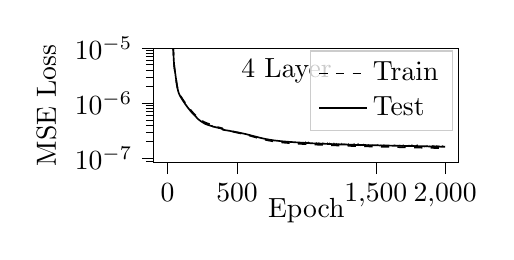
\begin{tikzpicture}

\begin{axis}[
legend cell align={left},
legend style={fill opacity=0.8, draw opacity=1, text opacity=1, draw=white!80!black},
log basis y={10},
tick align=outside,
tick pos=left,
title={4 Layer $\rare$},
title style={at={(0.45,0.85)},anchor=north},
x grid style={white!69.0196078431373!black},
xlabel={Epoch},
x label style={yshift=10pt},
xmin=-99.95, xmax=2098.95,
xtick style={color=black},
xtick = {0,500,1500,2000},
y grid style={white!69.0196078431373!black},
ylabel={MSE Loss},
ymin=8.43938809238065e-08, ymax=1e-5,
ymode=log,
ytick style={color=black},
width=.45\textwidth,
height=.25\textwidth
]
\addplot [semithick, black, dashed]
table {%
0 0.0216106624007225
1 0.00673290289845318
2 0.00242847194336355
3 0.00139278739271685
4 0.000877979734446853
5 0.000474738540826365
6 0.000281054378283443
7 0.00021271777068614
8 0.000184169041807763
9 0.000169510987921967
10 0.000160570089246903
11 0.000153623172860534
12 0.000146821876085596
13 0.000139312337923911
14 0.000130708834607503
15 0.000120814576126577
16 0.000109637301975454
17 9.74004520030576e-05
18 8.46704687937745e-05
19 7.22209239793301e-05
20 6.08980650031299e-05
21 5.13222632107499e-05
22 4.36849454090407e-05
23 3.78588456642319e-05
24 3.35587738209142e-05
25 3.04345663553249e-05
26 2.81585673401423e-05
27 2.64713321785166e-05
28 2.51700294393231e-05
29 2.40990629854423e-05
30 2.31376955125597e-05
31 2.21966665994842e-05
32 2.12135114788907e-05
33 2.01455304168121e-05
34 1.89702411180406e-05
35 1.76808702226481e-05
36 1.62871305710723e-05
37 1.48123448534534e-05
38 1.32958351109664e-05
39 1.17858424450787e-05
40 1.0341288148993e-05
41 9.02308400145557e-06
42 7.88079028029642e-06
43 6.9382161775593e-06
44 6.18492073954258e-06
45 5.61335765496551e-06
46 5.18214040664589e-06
47 4.851168252344e-06
48 4.5908486360986e-06
49 4.37404542492459e-06
50 4.1860971711003e-06
51 4.01634194429334e-06
52 3.85815369747888e-06
53 3.70789047474318e-06
54 3.56210532618206e-06
55 3.42163359334791e-06
56 3.28623007618489e-06
57 3.15185335739443e-06
58 3.0234138083074e-06
59 2.90046724973081e-06
60 2.78323152656412e-06
61 2.67022930574967e-06
62 2.56325708880922e-06
63 2.46282143962162e-06
64 2.36972090749532e-06
65 2.28372049502923e-06
66 2.20383440972682e-06
67 2.12981607876372e-06
68 2.0617129700895e-06
69 1.99959229286151e-06
70 1.94295511562359e-06
71 1.89111669618569e-06
72 1.84340184341636e-06
73 1.79986060237525e-06
74 1.75956733130533e-06
75 1.72281113952977e-06
76 1.68883256932872e-06
77 1.65757721526916e-06
78 1.62893817480381e-06
79 1.60244528660769e-06
80 1.57779333051167e-06
81 1.55488546303673e-06
82 1.53347499124834e-06
83 1.51332984992791e-06
84 1.49426139915931e-06
85 1.47615350221031e-06
86 1.45896057071582e-06
87 1.44265126846221e-06
88 1.42635903176824e-06
89 1.41095506359079e-06
90 1.39608382190204e-06
91 1.38187484546393e-06
92 1.3679947178673e-06
93 1.35463125761248e-06
94 1.34165614971948e-06
95 1.32878456537355e-06
96 1.31631478626559e-06
97 1.30407440371982e-06
98 1.29206818090211e-06
99 1.28030122669998e-06
100 1.26874039784752e-06
101 1.25744272938277e-06
102 1.24637065587763e-06
103 1.23556529459279e-06
104 1.22468484934757e-06
105 1.21391777702229e-06
106 1.20343351045449e-06
107 1.19293890546146e-06
108 1.18257735414318e-06
109 1.17147049024879e-06
110 1.16113315289113e-06
111 1.15103359098612e-06
112 1.14106687107096e-06
113 1.13130547171636e-06
114 1.12164716841789e-06
115 1.11212452972609e-06
116 1.10274103678876e-06
117 1.09347531545723e-06
118 1.08429839545465e-06
119 1.07525509415041e-06
120 1.06630471557878e-06
121 1.05751132139176e-06
122 1.0487439832616e-06
123 1.04011279623251e-06
124 1.03160096955435e-06
125 1.02322621967232e-06
126 1.01492625211108e-06
127 1.00679528438263e-06
128 9.98749102421925e-07
129 9.90614294664738e-07
130 9.82658809448367e-07
131 9.74852750289301e-07
132 9.67159750558721e-07
133 9.59597950853208e-07
134 9.52112600600685e-07
135 9.4466021650419e-07
136 9.37624845334994e-07
137 9.30101956882368e-07
138 9.2261810858929e-07
139 9.15006883133174e-07
140 9.07406760788376e-07
141 9.00099601224724e-07
142 8.92701309766153e-07
143 8.85610241880386e-07
144 8.78771238845388e-07
145 8.72219110959804e-07
146 8.65594072266163e-07
147 8.59149445574303e-07
148 8.52838356223629e-07
149 8.46545972649437e-07
150 8.40331516357651e-07
151 8.34286911057802e-07
152 8.28214898177748e-07
153 8.22116376156146e-07
154 8.16204172863877e-07
155 8.10378548209201e-07
156 8.04656332050513e-07
157 7.99051991762667e-07
158 7.93543244043349e-07
159 7.88110822099952e-07
160 7.82816938922792e-07
161 7.77351807641935e-07
162 7.72005825297129e-07
163 7.66674001397405e-07
164 7.61450602340119e-07
165 7.56337212166613e-07
166 7.5132788563792e-07
167 7.46323605710586e-07
168 7.41613327960522e-07
169 7.36650454257415e-07
170 7.31902793432937e-07
171 7.27025475512733e-07
172 7.22359442249854e-07
173 7.177709151307e-07
174 7.13255188415474e-07
175 7.08742484775371e-07
176 7.03956646006532e-07
177 6.98618378038418e-07
178 6.93606436271921e-07
179 6.88884985976301e-07
180 6.84381060153783e-07
181 6.80145616499317e-07
182 6.75724589797255e-07
183 6.71580819329165e-07
184 6.6738621748641e-07
185 6.6328372876967e-07
186 6.59295098714097e-07
187 6.55370623690032e-07
188 6.51456420968088e-07
189 6.4768271292337e-07
190 6.43534997621487e-07
191 6.39708978283693e-07
192 6.359301758323e-07
193 6.32180300485175e-07
194 6.28438367741069e-07
195 6.24702582612713e-07
196 6.21174068299979e-07
197 6.17387885085918e-07
198 6.1360695735857e-07
199 6.09839239018584e-07
200 6.06011450102528e-07
201 6.02128856996842e-07
202 5.98357907904301e-07
203 5.9438991659988e-07
204 5.90488967759484e-07
205 5.86552403930796e-07
206 5.82735191478889e-07
207 5.7880083262063e-07
208 5.7500634336094e-07
209 5.71188780483567e-07
210 5.67494936362323e-07
211 5.63854762901883e-07
212 5.60381861106407e-07
213 5.57017742153221e-07
214 5.53732854783107e-07
215 5.50645551413709e-07
216 5.47619643711528e-07
217 5.44531466303511e-07
218 5.41552928794431e-07
219 5.38660903046662e-07
220 5.35860492874463e-07
221 5.33061054838413e-07
222 5.30413544254316e-07
223 5.27592542923117e-07
224 5.25051639684193e-07
225 5.22539969892932e-07
226 5.20097590815283e-07
227 5.17746779479467e-07
228 5.15497621826455e-07
229 5.13201537245322e-07
230 5.10952482173366e-07
231 5.08788757684897e-07
232 5.06413795463345e-07
233 5.04197328794476e-07
234 5.02117503565103e-07
235 5.00099920714092e-07
236 4.98156201281574e-07
237 4.96120355620633e-07
238 4.94286574834746e-07
239 4.92361857155288e-07
240 4.90496158661813e-07
241 4.88675696999508e-07
242 4.86913171407366e-07
243 4.851756119848e-07
244 4.83470957902909e-07
245 4.81814274188253e-07
246 4.80199573651419e-07
247 4.78683203567698e-07
248 4.77044099817192e-07
249 4.75468882626728e-07
250 4.73879091153151e-07
251 4.72371058982901e-07
252 4.70842513635716e-07
253 4.6937632956201e-07
254 4.67929217776941e-07
255 4.66513790627232e-07
256 4.65088764485699e-07
257 4.6366257139141e-07
258 4.62334256909003e-07
259 4.60908514426706e-07
260 4.59539256539188e-07
261 4.582419610486e-07
262 4.56966788391355e-07
263 4.55675070149653e-07
264 4.54337393499316e-07
265 4.53071155732232e-07
266 4.51853715723871e-07
267 4.50666905862818e-07
268 4.49487872209886e-07
269 4.48350553412524e-07
270 4.47203686391617e-07
271 4.46084542019776e-07
272 4.44943811899634e-07
273 4.43894103753451e-07
274 4.42781260545644e-07
275 4.4177846840654e-07
276 4.40752303987324e-07
277 4.3963250649881e-07
278 4.38508849981645e-07
279 4.37525406496775e-07
280 4.36493751188038e-07
281 4.35531963482561e-07
282 4.34462244669476e-07
283 4.33431620805891e-07
284 4.32435458542102e-07
285 4.31482845442588e-07
286 4.30554591901e-07
287 4.29638015788214e-07
288 4.28745323013402e-07
289 4.2790234015655e-07
290 4.27039721159872e-07
291 4.26191598307923e-07
292 4.25355553360873e-07
293 4.24506018333659e-07
294 4.23655542931556e-07
295 4.22808301834721e-07
296 4.21996215266063e-07
297 4.21198938262535e-07
298 4.20371942965403e-07
299 4.19587211652583e-07
300 4.18860521804731e-07
301 4.18094755104903e-07
302 4.17349502271236e-07
303 4.16623433551422e-07
304 4.15895910307995e-07
305 4.15184494542586e-07
306 4.14479024385628e-07
307 4.13734667318977e-07
308 4.13033298542587e-07
309 4.12367151128024e-07
310 4.11671337289476e-07
311 4.11018487042725e-07
312 4.10363574829375e-07
313 4.09771400768477e-07
314 4.09135555258899e-07
315 4.08534289007889e-07
316 4.07766801657772e-07
317 4.07205162758828e-07
318 4.06719284313795e-07
319 4.05979226258069e-07
320 4.05369681857337e-07
321 4.04813660580317e-07
322 4.0424221703006e-07
323 4.01775835342733e-07
324 3.9732308940188e-07
325 3.95490883548177e-07
326 3.93727580572545e-07
327 3.9239304535954e-07
328 3.91342631729685e-07
329 3.90330171711639e-07
330 3.89447076273086e-07
331 3.88699826885386e-07
332 3.87784748724584e-07
333 3.87108554747329e-07
334 3.86313853951492e-07
335 3.85547236177786e-07
336 3.84728025963454e-07
337 3.83967091067916e-07
338 3.83136319840105e-07
339 3.82331433002037e-07
340 3.81500545188373e-07
341 3.80685198756225e-07
342 3.80033054341311e-07
343 3.79316259142115e-07
344 3.78621012487201e-07
345 3.7795977845434e-07
346 3.77288775951001e-07
347 3.76653722184983e-07
348 3.75958665728149e-07
349 3.75355292362656e-07
350 3.74698903961246e-07
351 3.74061793934288e-07
352 3.73468358191076e-07
353 3.72811548963625e-07
354 3.72241171824328e-07
355 3.71634515659025e-07
356 3.70998225157848e-07
357 3.70405478889779e-07
358 3.69798000349419e-07
359 3.69194266880868e-07
360 3.68567208624881e-07
361 3.679934441152e-07
362 3.67422204163859e-07
363 3.66914002796648e-07
364 3.66252508641196e-07
365 3.65631194782168e-07
366 3.65033643291213e-07
367 3.6445641813998e-07
368 3.63884713749485e-07
369 3.6333000007005e-07
370 3.62738613333136e-07
371 3.62184976779645e-07
372 3.61609488692238e-07
373 3.61079528076402e-07
374 3.60510225192456e-07
375 3.59959687756373e-07
376 3.59414541676983e-07
377 3.58882117126313e-07
378 3.58320710986959e-07
379 3.57816574023673e-07
380 3.5727768839422e-07
381 3.56719101432645e-07
382 3.56145097327953e-07
383 3.55607541536074e-07
384 3.55104071616097e-07
385 3.54350894710365e-07
386 3.53832532411502e-07
387 3.53362483537012e-07
388 3.52820708798163e-07
389 3.52301250558185e-07
390 3.51839069267612e-07
391 3.51369276515356e-07
392 3.50713634929889e-07
393 3.50198180385064e-07
394 3.42994273879071e-07
395 3.37459253060501e-07
396 3.36289835345838e-07
397 3.35470516276359e-07
398 3.34717947012564e-07
399 3.34036376955282e-07
400 3.33413894921364e-07
401 3.32775672802654e-07
402 3.32222780471625e-07
403 3.31656370008204e-07
404 3.31059441123216e-07
405 3.30471022579104e-07
406 3.29948070614705e-07
407 3.29408178927793e-07
408 3.28830659569235e-07
409 3.28420155582876e-07
410 3.27948691108304e-07
411 3.27466074267591e-07
412 3.26983534591818e-07
413 3.26529947187737e-07
414 3.26056213680204e-07
415 3.25601777944939e-07
416 3.25140297491089e-07
417 3.24708497444703e-07
418 3.24223424328807e-07
419 3.23786114506675e-07
420 3.23332559105438e-07
421 3.22898877939792e-07
422 3.22457123729691e-07
423 3.22002698311508e-07
424 3.21506677451566e-07
425 3.21149641436591e-07
426 3.2071827259017e-07
427 3.20318631850114e-07
428 3.19890345039653e-07
429 3.19473695739703e-07
430 3.18698119528449e-07
431 3.18401096876642e-07
432 3.17974057793435e-07
433 3.17500140937454e-07
434 3.17058012129223e-07
435 3.16648788057705e-07
436 3.16250691852815e-07
437 3.15829835571435e-07
438 3.15423972210738e-07
439 3.15066943116449e-07
440 3.14667640367361e-07
441 3.14271113822429e-07
442 3.13797254975157e-07
443 3.13497316142275e-07
444 3.13078043916448e-07
445 3.12755185831293e-07
446 3.12391271933166e-07
447 3.1198606302496e-07
448 3.1160391039009e-07
449 3.11256480088673e-07
450 3.10887099558954e-07
451 3.10662238675263e-07
452 3.10277672426196e-07
453 3.09896373551055e-07
454 3.09517824987893e-07
455 3.09143135638124e-07
456 3.08770616982201e-07
457 3.08405447086102e-07
458 3.08032719928519e-07
459 3.07656596632455e-07
460 3.07311306372071e-07
461 3.06948595408585e-07
462 3.06615132117827e-07
463 3.06262616817321e-07
464 3.05897978648773e-07
465 3.05542331858533e-07
466 3.05163595825775e-07
467 3.04796437418986e-07
468 3.04440751691004e-07
469 3.04076373026874e-07
470 3.03719222827681e-07
471 3.03353062221845e-07
472 3.02990892649291e-07
473 3.0263301108846e-07
474 3.02271752175898e-07
475 3.01934635672296e-07
476 3.0156328080011e-07
477 3.01179149317932e-07
478 3.00842650105437e-07
479 3.00472060928314e-07
480 3.00037528703001e-07
481 2.99667246835611e-07
482 2.99302288965464e-07
483 2.98947667644711e-07
484 2.98582195583208e-07
485 2.98215010573699e-07
486 2.9785535068072e-07
487 2.97490581374404e-07
488 2.97126231615152e-07
489 2.96774992690985e-07
490 2.96397045090657e-07
491 2.96061390230307e-07
492 2.95681678281312e-07
493 2.9532954511069e-07
494 2.94962441074631e-07
495 2.94596214985177e-07
496 2.94228129320118e-07
497 2.93864728405424e-07
498 2.93508675170528e-07
499 2.93143504279669e-07
500 2.92784303780991e-07
501 2.92416588507649e-07
502 2.92051301343577e-07
503 2.91686755957699e-07
504 2.91287320621336e-07
505 2.90917487433262e-07
506 2.90549759711212e-07
507 2.90181204320561e-07
508 2.89812056109895e-07
509 2.89444514450565e-07
510 2.89075045500908e-07
511 2.88704543976337e-07
512 2.88336096332387e-07
513 2.8796272732734e-07
514 2.87592303521933e-07
515 2.87219270418859e-07
516 2.86848664543982e-07
517 2.86476573634786e-07
518 2.86102311221725e-07
519 2.85724018624478e-07
520 2.85357762265903e-07
521 2.84981645876314e-07
522 2.8461455055151e-07
523 2.8425328021342e-07
524 2.83887521433712e-07
525 2.83510480073801e-07
526 2.83132329769842e-07
527 2.82761600246317e-07
528 2.82383754637294e-07
529 2.82003369363792e-07
530 2.81624365769062e-07
531 2.81253791044378e-07
532 2.80863522320374e-07
533 2.80491489519363e-07
534 2.80108860522432e-07
535 2.79729500917369e-07
536 2.79344856437547e-07
537 2.78964073430643e-07
538 2.78581386027099e-07
539 2.78189427277198e-07
540 2.77800684699514e-07
541 2.77422164160157e-07
542 2.77025935531583e-07
543 2.76675719604214e-07
544 2.7628835702842e-07
545 2.75891499214254e-07
546 2.754996529859e-07
547 2.7510834667055e-07
548 2.7471418212599e-07
549 2.74250312244817e-07
550 2.73937980210803e-07
551 2.73469895518019e-07
552 2.73089561275697e-07
553 2.72698263458437e-07
554 2.72312604806757e-07
555 2.71926184367999e-07
556 2.71536050803434e-07
557 2.71139314662605e-07
558 2.70746581449544e-07
559 2.70352984330202e-07
560 2.69956387015213e-07
561 2.69561034599519e-07
562 2.69184922245813e-07
563 2.68785443537922e-07
564 2.68388820202858e-07
565 2.67988743360092e-07
566 2.67580664214506e-07
567 2.6718646597601e-07
568 2.66785075979215e-07
569 2.66419031149212e-07
570 2.66015551616761e-07
571 2.65620774769104e-07
572 2.65219328838384e-07
573 2.64824864359525e-07
574 2.64434130130553e-07
575 2.64023973286953e-07
576 2.63620257200614e-07
577 2.63219747282051e-07
578 2.62736836447175e-07
579 2.62318192085331e-07
580 2.61909523416648e-07
581 2.61502716469408e-07
582 2.61105529247629e-07
583 2.60702718719585e-07
584 2.6029890841528e-07
585 2.59889832378235e-07
586 2.59486747424376e-07
587 2.59076840677608e-07
588 2.58672434839013e-07
589 2.58264190520663e-07
590 2.57854916384304e-07
591 2.57446017087659e-07
592 2.57047310228131e-07
593 2.56630037597461e-07
594 2.56229556200083e-07
595 2.55818167815391e-07
596 2.55413956594452e-07
597 2.55009213333324e-07
598 2.54611830413864e-07
599 2.54200633449386e-07
600 2.5380529264396e-07
601 2.53393371764332e-07
602 2.52922564399682e-07
603 2.52380531748031e-07
604 2.51938129494533e-07
605 2.5150760473025e-07
606 2.51107723556743e-07
607 2.50692401550623e-07
608 2.50296422933616e-07
609 2.49886340895955e-07
610 2.49492911265747e-07
611 2.49087333429543e-07
612 2.48680714250327e-07
613 2.48284265978782e-07
614 2.4788667600717e-07
615 2.47456508517985e-07
616 2.47051033085199e-07
617 2.46647489134944e-07
618 2.4625732633865e-07
619 2.45860469803461e-07
620 2.45425408920141e-07
621 2.45022914640458e-07
622 2.44652590524197e-07
623 2.44252181644811e-07
624 2.43862469332612e-07
625 2.43488337133613e-07
626 2.43087162303368e-07
627 2.42683210387895e-07
628 2.42284148342264e-07
629 2.4189684177145e-07
630 2.41453110305656e-07
631 2.4105597925228e-07
632 2.40666493098729e-07
633 2.402901326235e-07
634 2.39877828683177e-07
635 2.39510399850928e-07
636 2.39118784641335e-07
637 2.38734965940068e-07
638 2.38333517231126e-07
639 2.37971021149974e-07
640 2.37577484739404e-07
641 2.37201121635167e-07
642 2.36807600217048e-07
643 2.36442187372177e-07
644 2.36048477418649e-07
645 2.35720507248516e-07
646 2.3529685198298e-07
647 2.34926964964188e-07
648 2.34651763484806e-07
649 2.34295619804925e-07
650 2.33907534919808e-07
651 2.33553717706059e-07
652 2.33175521088924e-07
653 2.32825393268854e-07
654 2.32450461304268e-07
655 2.32095179185876e-07
656 2.31748523042086e-07
657 2.31385499631642e-07
658 2.31015129955381e-07
659 2.30663613251636e-07
660 2.30288796053912e-07
661 2.29934373187746e-07
662 2.29571597571976e-07
663 2.29216760359918e-07
664 2.28852116933354e-07
665 2.28495701144027e-07
666 2.28147498418707e-07
667 2.27798743303254e-07
668 2.27462652588883e-07
669 2.27117970155177e-07
670 2.26760281407223e-07
671 2.26418564309938e-07
672 2.26108651581569e-07
673 2.25791860522406e-07
674 2.25436486502417e-07
675 2.25098220347775e-07
676 2.24788045336766e-07
677 2.24459609604821e-07
678 2.24133774658242e-07
679 2.23800147416853e-07
680 2.23474523565415e-07
681 2.23188974956656e-07
682 2.2284166180242e-07
683 2.2254372058228e-07
684 2.22211433126063e-07
685 2.21920742731641e-07
686 2.21595553426823e-07
687 2.21314227367486e-07
688 2.21033817595639e-07
689 2.20716097487639e-07
690 2.20356926739385e-07
691 2.2009933127265e-07
692 2.19786205256867e-07
693 2.19499166888681e-07
694 2.19210622162791e-07
695 2.18931428264568e-07
696 2.18612988660993e-07
697 2.18332271472832e-07
698 2.18054914128629e-07
699 2.17747560832038e-07
700 2.17494242413352e-07
701 2.17189853188415e-07
702 2.16910481917409e-07
703 2.16647721089203e-07
704 2.16394595852876e-07
705 2.1610913848491e-07
706 2.15835460842584e-07
707 2.15616975424382e-07
708 2.15359850656682e-07
709 2.15075565435541e-07
710 2.14831694350437e-07
711 2.14503112900388e-07
712 2.14279591034483e-07
713 2.13987736259469e-07
714 2.13740835725673e-07
715 2.13455635510229e-07
716 2.13242247525614e-07
717 2.12986595641951e-07
718 2.12713128561859e-07
719 2.12486485366981e-07
720 2.12225340455063e-07
721 2.11995605106097e-07
722 2.11794130493104e-07
723 2.11524806914554e-07
724 2.1125673990241e-07
725 2.11031820846586e-07
726 2.1081890638186e-07
727 2.10560273671945e-07
728 2.10315091813129e-07
729 2.10102463988449e-07
730 2.09889895714355e-07
731 2.09609642865871e-07
732 2.09425779999606e-07
733 2.09183616597386e-07
734 2.08990658443042e-07
735 2.08729989289225e-07
736 2.08531867073702e-07
737 2.08309944277119e-07
738 2.08086278355779e-07
739 2.0789459659909e-07
740 2.07680310651881e-07
741 2.0747119165776e-07
742 2.07236777498565e-07
743 2.07018175132134e-07
744 2.06816486773675e-07
745 2.06584763589035e-07
746 2.06387027432697e-07
747 2.06218926180668e-07
748 2.06005806859366e-07
749 2.05752826182959e-07
750 2.05548594330196e-07
751 2.05311775921757e-07
752 2.05142609736697e-07
753 2.0495073572846e-07
754 2.04771630293976e-07
755 2.0461071154898e-07
756 2.04373782693779e-07
757 2.04192100383693e-07
758 2.04031139503513e-07
759 2.03814531289481e-07
760 2.03654313601476e-07
761 2.03442323652325e-07
762 2.03277292598614e-07
763 2.0309212533931e-07
764 2.02949136372865e-07
765 2.02724689088996e-07
766 2.02560473084645e-07
767 2.02350404919116e-07
768 2.02225088422381e-07
769 2.02075813668046e-07
770 2.01815807457706e-07
771 2.01668591600423e-07
772 2.01510255024573e-07
773 2.01304897409216e-07
774 2.01147469894636e-07
775 2.0087547069636e-07
776 2.00708041205644e-07
777 2.00552844987101e-07
778 2.00407669666447e-07
779 2.00212583891357e-07
780 2.00079323661839e-07
781 1.99906171182818e-07
782 1.99735537769641e-07
783 1.99590529170734e-07
784 1.99458949076359e-07
785 1.9929100927385e-07
786 1.99101222690956e-07
787 1.98979387548093e-07
788 1.9883520160846e-07
789 1.98662458501531e-07
790 1.98509994092433e-07
791 1.98378701213642e-07
792 1.98230722041615e-07
793 1.98054001302239e-07
794 1.97913957400431e-07
795 1.97748915866214e-07
796 1.97619246243619e-07
797 1.97458854394483e-07
798 1.9732037737441e-07
799 1.9718832942317e-07
800 1.97041426808653e-07
801 1.96902047633785e-07
802 1.96766920048219e-07
803 1.96604294650626e-07
804 1.96496536219115e-07
805 1.96382572973164e-07
806 1.96219839480705e-07
807 1.96085320837369e-07
808 1.95963470162042e-07
809 1.95823555152685e-07
810 1.95713456996316e-07
811 1.95573616785794e-07
812 1.95453819671343e-07
813 1.95311064544512e-07
814 1.95212965564906e-07
815 1.95100162919459e-07
816 1.94962750249772e-07
817 1.94830665954271e-07
818 1.94717411517331e-07
819 1.94620832374426e-07
820 1.94458740004677e-07
821 1.94354109922301e-07
822 1.94270007597197e-07
823 1.94124745341639e-07
824 1.94010768659325e-07
825 1.93872416154761e-07
826 1.93788308628484e-07
827 1.93651885346924e-07
828 1.93532121421924e-07
829 1.93444749363891e-07
830 1.93306050924491e-07
831 1.93204075095821e-07
832 1.9309011060642e-07
833 1.92993874705394e-07
834 1.92862723380927e-07
835 1.92772320488643e-07
836 1.92665639630718e-07
837 1.92546770804825e-07
838 1.92435405381275e-07
839 1.92352559281517e-07
840 1.92240041741343e-07
841 1.92133511006887e-07
842 1.92020548425376e-07
843 1.919115628084e-07
844 1.91812710554018e-07
845 1.91718293251597e-07
846 1.91616724755761e-07
847 1.91497081054592e-07
848 1.91413476578362e-07
849 1.91311501069436e-07
850 1.91188739904646e-07
851 1.91130697771769e-07
852 1.91013988590782e-07
853 1.90901197811399e-07
854 1.90812814622632e-07
855 1.90715631696037e-07
856 1.90646210654677e-07
857 1.90514590059365e-07
858 1.90444030131687e-07
859 1.90331704054358e-07
860 1.90250029120875e-07
861 1.90143055029068e-07
862 1.90024863513827e-07
863 1.89974942529147e-07
864 1.89862021365173e-07
865 1.89752594678794e-07
866 1.89691171975426e-07
867 1.89590054446853e-07
868 1.89481359015531e-07
869 1.89564498441541e-07
870 1.89266790783904e-07
871 1.89147045318805e-07
872 1.89083462664996e-07
873 1.89025151307476e-07
874 1.88914466036749e-07
875 1.88806591928881e-07
876 1.88748112037729e-07
877 1.88681913918742e-07
878 1.88565463105306e-07
879 1.88473345332341e-07
880 1.88422301071967e-07
881 1.88273862789856e-07
882 1.88229817830177e-07
883 1.88129125866965e-07
884 1.88074489372525e-07
885 1.87977990435684e-07
886 1.87873305492303e-07
887 1.87809109206682e-07
888 1.87705275983774e-07
889 1.87653425115286e-07
890 1.87576660152899e-07
891 1.87455449136564e-07
892 1.8739126468148e-07
893 1.87289279985237e-07
894 1.8724850141183e-07
895 1.87153168901943e-07
896 1.8706308216565e-07
897 1.86987817727413e-07
898 1.86928051377322e-07
899 1.86846638250415e-07
900 1.86764167771969e-07
901 1.86676254728013e-07
902 1.86577274298827e-07
903 1.86536912949009e-07
904 1.8646056668814e-07
905 1.86386593952648e-07
906 1.86291404176586e-07
907 1.86223032379473e-07
908 1.86134376484404e-07
909 1.86082618697014e-07
910 1.85978073758974e-07
911 1.85938494226434e-07
912 1.85864153408488e-07
913 1.85785363839841e-07
914 1.85678791211785e-07
915 1.85629285340383e-07
916 1.85553920864834e-07
917 1.85486233405641e-07
918 1.8540947337442e-07
919 1.85350580267141e-07
920 1.85271162948197e-07
921 1.85202297849685e-07
922 1.85131175925335e-07
923 1.85051926912649e-07
924 1.84978863472907e-07
925 1.8492998484021e-07
926 1.84832688674419e-07
927 1.84801209300645e-07
928 1.84736455373979e-07
929 1.84623548165064e-07
930 1.84608434793176e-07
931 1.84504162469068e-07
932 1.84435943999972e-07
933 1.84360517607729e-07
934 1.84322198350628e-07
935 1.84215514472896e-07
936 1.84190147251684e-07
937 1.84140666071642e-07
938 1.84041638341625e-07
939 1.83968719234429e-07
940 1.83896355849811e-07
941 1.83837361070971e-07
942 1.83839822845755e-07
943 1.83766977229993e-07
944 1.83638415258258e-07
945 1.83566072095687e-07
946 1.83519504091123e-07
947 1.83446028835021e-07
948 1.83395068596326e-07
949 1.83316212236662e-07
950 1.83285562606272e-07
951 1.83199140721513e-07
952 1.83183291241562e-07
953 1.83075190882676e-07
954 1.83062210787455e-07
955 1.82927106422426e-07
956 1.82892595525175e-07
957 1.82834764522966e-07
958 1.82783786037533e-07
959 1.82701763108639e-07
960 1.82646872232795e-07
961 1.82573253077578e-07
962 1.82511307478705e-07
963 1.82460096070258e-07
964 1.82422018170314e-07
965 1.82331821022785e-07
966 1.82296495310652e-07
967 1.82236372658906e-07
968 1.8213447961557e-07
969 1.8208163304223e-07
970 1.82025621178639e-07
971 1.81966136040046e-07
972 1.81946712665138e-07
973 1.81872313675058e-07
974 1.81773238892902e-07
975 1.81758913051056e-07
976 1.8167523741397e-07
977 1.81603671109087e-07
978 1.81574254867201e-07
979 1.81481448350951e-07
980 1.8144391169983e-07
981 1.81378839940294e-07
982 1.81291478270396e-07
983 1.81267837923826e-07
984 1.81212172982725e-07
985 1.81145498459045e-07
986 1.81104971638035e-07
987 1.81015536654172e-07
988 1.81003275883995e-07
989 1.80951426081322e-07
990 1.80898478369329e-07
991 1.80804848220362e-07
992 1.80737904678097e-07
993 1.80692982183928e-07
994 1.8063039879479e-07
995 1.80686602881508e-07
996 1.80568369920309e-07
997 1.80461264832843e-07
998 1.80398518651259e-07
999 1.80379310890544e-07
1000 1.80326845374168e-07
1001 1.80228571188934e-07
1002 1.80212151668968e-07
1003 1.80164973421881e-07
1004 1.80055146493885e-07
1005 1.80016070551403e-07
1006 1.80035480369156e-07
1007 1.79911012459399e-07
1008 1.79842733800228e-07
1009 1.79833708145338e-07
1010 1.79744951807947e-07
1011 1.79718168539011e-07
1012 1.79695514212597e-07
1013 1.79632579659028e-07
1014 1.7958827668707e-07
1015 1.79485900808629e-07
1016 1.79413860877276e-07
1017 1.79370492290332e-07
1018 1.79360341761026e-07
1019 1.79332420671585e-07
1020 1.79230263661623e-07
1021 1.7917569885384e-07
1022 1.79127057556627e-07
1023 1.79241113549722e-07
1024 1.7917623971897e-07
1025 1.79244382202626e-07
1026 1.79210308260735e-07
1027 1.79150409216788e-07
1028 1.79036714634151e-07
1029 1.79027852738045e-07
1030 1.78958927357087e-07
1031 1.7893335813568e-07
1032 1.78864548978197e-07
1033 1.78835367890429e-07
1034 1.78795579536484e-07
1035 1.78755134868425e-07
1036 1.78641936344093e-07
1037 1.78593477691891e-07
1038 1.78590952224056e-07
1039 1.78499820442823e-07
1040 1.78439640791339e-07
1041 1.78394428537842e-07
1042 1.78378901708243e-07
1043 1.78302251427453e-07
1044 1.78258820334065e-07
1045 1.78191099934111e-07
1046 1.78159377298925e-07
1047 1.78104258438339e-07
1048 1.78057871373483e-07
1049 1.78015181447222e-07
1050 1.77944034774669e-07
1051 1.77941957588246e-07
1052 1.77853626396995e-07
1053 1.77814524832343e-07
1054 1.7774813699134e-07
1055 1.77703809889351e-07
1056 1.77675952258483e-07
1057 1.77648358352656e-07
1058 1.77571942579391e-07
1059 1.77527472061456e-07
1060 1.77485991635251e-07
1061 1.7744707773204e-07
1062 1.77386032802929e-07
1063 1.77322587973094e-07
1064 1.77299124445085e-07
1065 1.77234235543722e-07
1066 1.77215259405727e-07
1067 1.77158344335737e-07
1068 1.77124247471738e-07
1069 1.77064489179202e-07
1070 1.76985912368366e-07
1071 1.76983701834388e-07
1072 1.76910187533963e-07
1073 1.76876028099571e-07
1074 1.76824726956681e-07
1075 1.76798676029932e-07
1076 1.76776226531672e-07
1077 1.76694430521707e-07
1078 1.76621351180017e-07
1079 1.76610401460664e-07
1080 1.76574187129575e-07
1081 1.7649910562767e-07
1082 1.76468546882802e-07
1083 1.76431862030313e-07
1084 1.7638737516279e-07
1085 1.76306908748813e-07
1086 1.76277939857528e-07
1087 1.76302373539272e-07
1088 1.7617569829298e-07
1089 1.76178361300572e-07
1090 1.76133429633296e-07
1091 1.76041002141858e-07
1092 1.75977817043815e-07
1093 1.75944437359021e-07
1094 1.75941254248357e-07
1095 1.75881839190595e-07
1096 1.75846790924084e-07
1097 1.75819223144913e-07
1098 1.75713790490306e-07
1099 1.75664444050483e-07
1100 1.75637258344352e-07
1101 1.75566675693517e-07
1102 1.75534115825826e-07
1103 1.75526750261668e-07
1104 1.75438703770681e-07
1105 1.7538309885623e-07
1106 1.75376762328483e-07
1107 1.7530193790094e-07
1108 1.75282633335883e-07
1109 1.75220648891639e-07
1110 1.75184468702128e-07
1111 1.75177809552451e-07
1112 1.75096959537768e-07
1113 1.75071028550633e-07
1114 1.75022347598031e-07
1115 1.7497661561805e-07
1116 1.74940363855569e-07
1117 1.74892061075127e-07
1118 1.74832643715206e-07
1119 1.74859169668196e-07
1120 1.74774426554336e-07
1121 1.7468253720665e-07
1122 1.74662733201103e-07
1123 1.74636310930509e-07
1124 1.74569058856378e-07
1125 1.74553399908461e-07
1126 1.74507346848429e-07
1127 1.74474903275268e-07
1128 1.74449821827238e-07
1129 1.74340132559792e-07
1130 1.74361761217767e-07
1131 1.74297626386988e-07
1132 1.74214229467395e-07
1133 1.74233699652859e-07
1134 1.7419528980156e-07
1135 1.74113174260526e-07
1136 1.74103606482845e-07
1137 1.74103460260255e-07
1138 1.73959555390013e-07
1139 1.73925013555731e-07
1140 1.7386210139847e-07
1141 1.73848528262965e-07
1142 1.73805815336436e-07
1143 1.73731946027544e-07
1144 1.73736144176928e-07
1145 1.73698482896612e-07
1146 1.73662524865392e-07
1147 1.73587405967623e-07
1148 1.73579918822497e-07
1149 1.73576758577099e-07
1150 1.735323319636e-07
1151 1.73485661129291e-07
1152 1.73443705548948e-07
1153 1.73351196750104e-07
1154 1.73381033533815e-07
1155 1.73310837986662e-07
1156 1.73295372221105e-07
1157 1.73259445723772e-07
1158 1.73227503879048e-07
1159 1.73195007207028e-07
1160 1.73187520424278e-07
1161 1.7306360564362e-07
1162 1.73050464432833e-07
1163 1.73035037157376e-07
1164 1.73087016712259e-07
1165 1.72968198214107e-07
1166 1.72881617530152e-07
1167 1.7295136483142e-07
1168 1.72851830512855e-07
1169 1.72818079022363e-07
1170 1.72778573158894e-07
1171 1.72718693640661e-07
1172 1.7270090534538e-07
1173 1.7270916892187e-07
1174 1.72568362536651e-07
1175 1.72577032891752e-07
1176 1.7258109477325e-07
1177 1.7260609226355e-07
1178 1.72448717250973e-07
1179 1.72415710743223e-07
1180 1.72395935955194e-07
1181 1.72397184961426e-07
1182 1.72349606657463e-07
1183 1.72301530355412e-07
1184 1.72214634403645e-07
1185 1.72153765760186e-07
1186 1.72193612456795e-07
1187 1.72204249409447e-07
1188 1.72087060846593e-07
1189 1.72026658063373e-07
1190 1.72075992630027e-07
1191 1.72030504209886e-07
1192 1.71926870820016e-07
1193 1.71936961912422e-07
1194 1.71891174524319e-07
1195 1.71880935219804e-07
1196 1.71827827792015e-07
1197 1.71822777382147e-07
1198 1.71786435757326e-07
1199 1.71768815185658e-07
1200 1.71702090860038e-07
1201 1.71739857854902e-07
1202 1.71617547074732e-07
1203 1.7156320400602e-07
1204 1.71528990875913e-07
1205 1.71517066888782e-07
1206 1.71513961973346e-07
1207 1.71403330170961e-07
1208 1.71346198889921e-07
1209 1.71383523543511e-07
1210 1.71362682102938e-07
1211 1.71336470835115e-07
1212 1.71251969312891e-07
1213 1.71174495115167e-07
1214 1.71233604270071e-07
1215 1.71314036798265e-07
1216 1.71165501981818e-07
1217 1.71071120618649e-07
1218 1.70984958153042e-07
1219 1.7098195895926e-07
1220 1.71015771975647e-07
1221 1.70996565053372e-07
1222 1.70884112144165e-07
1223 1.7089750729582e-07
1224 1.70790641050189e-07
1225 1.70798408198891e-07
1226 1.70828165650505e-07
1227 1.70793065173314e-07
1228 1.70700528443035e-07
1229 1.7067476072441e-07
1230 1.70675086287986e-07
1231 1.70612983040996e-07
1232 1.70565547598756e-07
1233 1.7050324265e-07
1234 1.70488775488309e-07
1235 1.70464546236815e-07
1236 1.70451107408098e-07
1237 1.70438943598583e-07
1238 1.70367497503321e-07
1239 1.70297669853881e-07
1240 1.70287840084882e-07
1241 1.70317440392864e-07
1242 1.70259187768806e-07
1243 1.70169387097019e-07
1244 1.70166060954102e-07
1245 1.7015959914346e-07
1246 1.70072879036809e-07
1247 1.70080203453438e-07
1248 1.69973099353626e-07
1249 1.70045703136168e-07
1250 1.69952917950411e-07
1251 1.69955662016719e-07
1252 1.69859973333075e-07
1253 1.69899801925055e-07
1254 1.69820288007827e-07
1255 1.69868564412923e-07
1256 1.69765343969175e-07
1257 1.69748448229257e-07
1258 1.69705800452391e-07
1259 1.6965306291894e-07
1260 1.69602442973371e-07
1261 1.69608080632599e-07
1262 1.69599682138255e-07
1263 1.69567798202763e-07
1264 1.69505588857533e-07
1265 1.69445060365092e-07
1266 1.69388760596689e-07
1267 1.69400478604587e-07
1268 1.69410320395968e-07
1269 1.69311620716428e-07
1270 1.69259400074395e-07
1271 1.69325856880675e-07
1272 1.69370852745487e-07
1273 1.69243204737768e-07
1274 1.69179619966542e-07
1275 1.69161871589552e-07
1276 1.69083306850837e-07
1277 1.69077230957271e-07
1278 1.69089837299907e-07
1279 1.69023000928803e-07
1280 1.69091059262882e-07
1281 1.68983588977767e-07
1282 1.68936555738242e-07
1283 1.68931953034246e-07
1284 1.68985705300884e-07
1285 1.68975296190865e-07
1286 1.68837971287417e-07
1287 1.68774838392949e-07
1288 1.68735167370926e-07
1289 1.68765960466999e-07
1290 1.68746516699514e-07
1291 1.68695649733763e-07
1292 1.68646468864608e-07
1293 1.68562413257689e-07
1294 1.6858988993107e-07
1295 1.68670126527104e-07
1296 1.68366325972613e-07
1297 1.6832450091897e-07
1298 1.68334291473116e-07
1299 1.68343839312968e-07
1300 1.68317190968992e-07
1301 1.68235172893105e-07
1302 1.68274554212644e-07
1303 1.68399181184498e-07
1304 1.68282554334098e-07
1305 1.68080057100894e-07
1306 1.68025432877528e-07
1307 1.68044797234757e-07
1308 1.68017354866379e-07
1309 1.67995841799495e-07
1310 1.68006798560327e-07
1311 1.67982508379794e-07
1312 1.67921054860187e-07
1313 1.67883917420397e-07
1314 1.67839464054964e-07
1315 1.67829756712479e-07
1316 1.67853974403442e-07
1317 1.67749433863662e-07
1318 1.67708428286062e-07
1319 1.67713444042761e-07
1320 1.67860712927848e-07
1321 1.67689125817105e-07
1322 1.67559621274904e-07
1323 1.67547872322871e-07
1324 1.67564348146243e-07
1325 1.67477222703383e-07
1326 1.67485049338723e-07
1327 1.67526131981788e-07
1328 1.6742998275987e-07
1329 1.67414902726648e-07
1330 1.6736702631448e-07
1331 1.67352104973872e-07
1332 1.67339367976638e-07
1333 1.6726915405485e-07
1334 1.67304407696633e-07
1335 1.67264324431926e-07
1336 1.67214283322892e-07
1337 1.67262341591368e-07
1338 1.67241847648825e-07
1339 1.67110093784117e-07
1340 1.67036057391101e-07
1341 1.67139857801146e-07
1342 1.67201785750137e-07
1343 1.66920922900715e-07
1344 1.66950420755541e-07
1345 1.66943121350016e-07
1346 1.66929704967345e-07
1347 1.66912089149207e-07
1348 1.66969160659392e-07
1349 1.66813377553865e-07
1350 1.66787883031816e-07
1351 1.66778691990999e-07
1352 1.66794166055695e-07
1353 1.66790056709942e-07
1354 1.66844713575642e-07
1355 1.66592245811614e-07
1356 1.66663042314497e-07
1357 1.66594229689565e-07
1358 1.66581775118857e-07
1359 1.66553394748803e-07
1360 1.66581533129317e-07
1361 1.66522043343775e-07
1362 1.66457377808626e-07
1363 1.66468092778871e-07
1364 1.66456248294367e-07
1365 1.66391937916899e-07
1366 1.6636954207172e-07
1367 1.66337186605858e-07
1368 1.66337999544908e-07
1369 1.66300411265752e-07
1370 1.66256585025337e-07
1371 1.66230324694538e-07
1372 1.66262054960953e-07
1373 1.66311842029643e-07
1374 1.6620884812113e-07
1375 1.66082737052875e-07
1376 1.66100138692116e-07
1377 1.66071855289829e-07
1378 1.65991287140343e-07
1379 1.66027292841875e-07
1380 1.66048765017024e-07
1381 1.65978204798023e-07
1382 1.65909461287583e-07
1383 1.65914692715319e-07
1384 1.65921796678958e-07
1385 1.65908610057386e-07
1386 1.6584075878967e-07
1387 1.65783007716414e-07
1388 1.65777221020846e-07
1389 1.65749755105082e-07
1390 1.65692761413538e-07
1391 1.65716249071579e-07
1392 1.65707926868208e-07
1393 1.65664443692037e-07
1394 1.65660392909217e-07
1395 1.6555531041007e-07
1396 1.65595974486621e-07
1397 1.65527711487812e-07
1398 1.65510852603745e-07
1399 1.65448139732405e-07
1400 1.65507440037516e-07
1401 1.65409376414516e-07
1402 1.65359866144854e-07
1403 1.65365921347416e-07
1404 1.65365050953881e-07
1405 1.65445104364892e-07
1406 1.65383935843977e-07
1407 1.65204668604702e-07
1408 1.65154134542433e-07
1409 1.65219209932843e-07
1410 1.65202215775651e-07
1411 1.6515671573103e-07
1412 1.65137949920791e-07
1413 1.65116417022659e-07
1414 1.6504532810302e-07
1415 1.65028859363758e-07
1416 1.6504706556475e-07
1417 1.64975679453505e-07
1418 1.64952036158184e-07
1419 1.64949861805042e-07
1420 1.64942287014469e-07
1421 1.64880639310638e-07
1422 1.64852907623469e-07
1423 1.64815023296683e-07
1424 1.64827068971363e-07
1425 1.6479692638427e-07
1426 1.64800686256683e-07
1427 1.64663229007544e-07
1428 1.64735067940569e-07
1429 1.64699877252872e-07
1430 1.64645984632727e-07
1431 1.64649042353915e-07
1432 1.64592018414567e-07
1433 1.64586802981148e-07
1434 1.64533369286346e-07
1435 1.64534088234802e-07
1436 1.64539180580903e-07
1437 1.64588025249657e-07
1438 1.64528626413585e-07
1439 1.64403049730311e-07
1440 1.64434569235539e-07
1441 1.64330305665317e-07
1442 1.64350557383841e-07
1443 1.64313907802693e-07
1444 1.64288167425752e-07
1445 1.64290333536599e-07
1446 1.64252259480691e-07
1447 1.64279479896834e-07
1448 1.6423641449137e-07
1449 1.64184464686912e-07
1450 1.64129400964441e-07
1451 1.64106395708075e-07
1452 1.64089033887649e-07
1453 1.64048898746216e-07
1454 1.64055080958292e-07
1455 1.64035842338706e-07
1456 1.64035157851572e-07
1457 1.63966343592392e-07
1458 1.6393386583502e-07
1459 1.63920002862028e-07
1460 1.63905486353144e-07
1461 1.63842626747623e-07
1462 1.63854071125513e-07
1463 1.63843182377832e-07
1464 1.63801519676099e-07
1465 1.63759081736714e-07
1466 1.63764028513924e-07
1467 1.63723978161556e-07
1468 1.63663750292642e-07
1469 1.63675580736822e-07
1470 1.63701325028853e-07
1471 1.63652787477986e-07
1472 1.63594848658022e-07
1473 1.63543358503659e-07
1474 1.63574874825656e-07
1475 1.63533181869013e-07
1476 1.63477860958494e-07
1477 1.63506070094854e-07
1478 1.6346910118159e-07
1479 1.63388968786649e-07
1480 1.63403992630151e-07
1481 1.63401504394756e-07
1482 1.63334911896129e-07
1483 1.63362521405475e-07
1484 1.63307964221815e-07
1485 1.63266157784392e-07
1486 1.63244747525937e-07
1487 1.63252576001582e-07
1488 1.63205464630778e-07
1489 1.6317926982623e-07
1490 1.63177952131832e-07
1491 1.63116752538883e-07
1492 1.63130517712773e-07
1493 1.63142071770039e-07
1494 1.63082057653696e-07
1495 1.63039829530476e-07
1496 1.62986418189348e-07
1497 1.63003632266623e-07
1498 1.6297419497846e-07
1499 1.62977809573306e-07
1500 1.62908251610361e-07
1501 1.62888266856953e-07
1502 1.62894972540073e-07
1503 1.6281705941168e-07
1504 1.62824144119611e-07
1505 1.62801411775604e-07
1506 1.62785903242479e-07
1507 1.62790458873019e-07
1508 1.62755779378188e-07
1509 1.62805195941473e-07
1510 1.62741083300943e-07
1511 1.62614733277167e-07
1512 1.62588511336992e-07
1513 1.62593399018363e-07
1514 1.62582695779179e-07
1515 1.62611406956614e-07
1516 1.62567546233561e-07
1517 1.62476563382086e-07
1518 1.62453610897728e-07
1519 1.62472841758188e-07
1520 1.62409258251728e-07
1521 1.62407369678874e-07
1522 1.62439174310691e-07
1523 1.62376711131174e-07
1524 1.62357890829412e-07
1525 1.62330951390288e-07
1526 1.62282029890548e-07
1527 1.62258464939669e-07
1528 1.62386171474793e-07
1529 1.62246081977457e-07
1530 1.62181757545454e-07
1531 1.6214893717148e-07
1532 1.62138087752339e-07
1533 1.6213818561539e-07
1534 1.62098755609463e-07
1535 1.62070517177426e-07
1536 1.62076942373801e-07
1537 1.62076044901482e-07
1538 1.62060141597919e-07
1539 1.61987526915652e-07
1540 1.61971739032651e-07
1541 1.61926232046028e-07
1542 1.61918721609311e-07
1543 1.61893961497128e-07
1544 1.6187512852639e-07
1545 1.61897783129916e-07
1546 1.6183849820095e-07
1547 1.61819013932529e-07
1548 1.61767674043745e-07
1549 1.61779257460637e-07
1550 1.61762891366379e-07
1551 1.61720912878138e-07
1552 1.61708021494178e-07
1553 1.61623495422702e-07
1554 1.61689888656724e-07
1555 1.61645654770837e-07
1556 1.61627561659827e-07
1557 1.61584144386495e-07
1558 1.61566055083995e-07
1559 1.61593238935609e-07
1560 1.6156369655107e-07
1561 1.61485519804216e-07
1562 1.6143838396232e-07
1563 1.61465926417748e-07
1564 1.61439363473903e-07
1565 1.61373608236204e-07
1566 1.61376746753206e-07
1567 1.61372395311332e-07
1568 1.61365052711915e-07
1569 1.61270477434528e-07
1570 1.61305438325599e-07
1571 1.6128386074854e-07
1572 1.6120980218659e-07
1573 1.61217556552629e-07
1574 1.61202849270126e-07
1575 1.61158415636464e-07
1576 1.61146072542806e-07
1577 1.61116594973976e-07
1578 1.61089867823705e-07
1579 1.61058869643682e-07
1580 1.61075818958523e-07
1581 1.60997869258495e-07
1582 1.60995202037384e-07
1583 1.60991695985047e-07
1584 1.60972638340695e-07
1585 1.60917201000643e-07
1586 1.60925989412419e-07
1587 1.6090620315623e-07
1588 1.60876287630174e-07
1589 1.60871587006284e-07
1590 1.608295123674e-07
1591 1.60810746869799e-07
1592 1.60792823564293e-07
1593 1.60731222976551e-07
1594 1.60725678398421e-07
1595 1.60743065173108e-07
1596 1.60692538059948e-07
1597 1.60662292991276e-07
1598 1.60687539874971e-07
1599 1.60647360310406e-07
1600 1.60643607117095e-07
1601 1.60562668689579e-07
1602 1.60560070440852e-07
1603 1.60531671774322e-07
1604 1.605189931837e-07
1605 1.60465122299058e-07
1606 1.60481532560652e-07
1607 1.60452848923853e-07
1608 1.60447297758992e-07
1609 1.60448149877368e-07
1610 1.60383949321385e-07
1611 1.60370203410309e-07
1612 1.60340380546131e-07
1613 1.60316806301353e-07
1614 1.60336975469022e-07
1615 1.60274468434807e-07
1616 1.60265671610205e-07
1617 1.60206146965436e-07
1618 1.6017395471124e-07
1619 1.6019242134746e-07
1620 1.60202111970875e-07
1621 1.60110613911968e-07
1622 1.60101618185138e-07
1623 1.60084186518361e-07
1624 1.60075974164897e-07
1625 1.60056341130144e-07
1626 1.60024469295195e-07
1627 1.60016861734391e-07
1628 1.5996215306302e-07
1629 1.59993971742267e-07
1630 1.59975415030544e-07
1631 1.59897546794241e-07
1632 1.59864979707436e-07
1633 1.5981264795073e-07
1634 1.59833385943386e-07
1635 1.59786259438022e-07
1636 1.5975959943404e-07
1637 1.59836109965283e-07
1638 1.59749508142681e-07
1639 1.59673018117701e-07
1640 1.59672461165883e-07
1641 1.59673905095303e-07
1642 1.59624695783123e-07
1643 1.59605662418016e-07
1644 1.59605513445626e-07
1645 1.59538471798726e-07
1646 1.59518216165111e-07
1647 1.59490265389195e-07
1648 1.59514611830502e-07
1649 1.59506289037381e-07
1650 1.594392940234e-07
1651 1.59437268926865e-07
1652 1.59391223355954e-07
1653 1.59379607872268e-07
1654 1.5933557291703e-07
1655 1.59336109298636e-07
1656 1.59273247241742e-07
1657 1.59280083103397e-07
1658 1.59303168210556e-07
1659 1.59266005447023e-07
1660 1.5923947286467e-07
1661 1.59195379566768e-07
1662 1.59185277276208e-07
1663 1.59162616085951e-07
1664 1.59113985738202e-07
1665 1.59115515032227e-07
1666 1.59078035096627e-07
1667 1.590620035401e-07
1668 1.59055500247973e-07
1669 1.59017629734137e-07
1670 1.59004733653489e-07
1671 1.58984582405708e-07
1672 1.5893618891738e-07
1673 1.58970893295418e-07
1674 1.58974270824785e-07
1675 1.58856075486824e-07
1676 1.58825552816211e-07
1677 1.5882929874067e-07
1678 1.58840414911765e-07
1679 1.58816994570543e-07
1680 1.58759385541885e-07
1681 1.58741842831489e-07
1682 1.587232752982e-07
1683 1.58727088788169e-07
1684 1.5868284273779e-07
1685 1.58663293703398e-07
1686 1.58653893663541e-07
1687 1.58617259465643e-07
1688 1.58564271245609e-07
1689 1.58562940306695e-07
1690 1.5858223643761e-07
1691 1.58529176921718e-07
1692 1.58498967628873e-07
1693 1.58529810825314e-07
1694 1.58439630631335e-07
1695 1.58456428877685e-07
1696 1.58413188358963e-07
1697 1.58366994817527e-07
1698 1.5844551713684e-07
1699 1.58414659182426e-07
1700 1.58323922740067e-07
1701 1.58267001054924e-07
1702 1.58278427797143e-07
1703 1.5828589792477e-07
1704 1.58217034922359e-07
1705 1.58233597289836e-07
1706 1.58217247403059e-07
1707 1.58180190943824e-07
1708 1.58171623702685e-07
1709 1.58144930544779e-07
1710 1.5814085011101e-07
1711 1.5810550590345e-07
1712 1.58071546813687e-07
1713 1.58090500818275e-07
1714 1.5802699835632e-07
1715 1.58003030328757e-07
1716 1.57996284798401e-07
1717 1.57944636079321e-07
1718 1.57902301893387e-07
1719 1.57958363530497e-07
1720 1.57928429686649e-07
1721 1.5788781043824e-07
1722 1.5786845246879e-07
1723 1.57857515972637e-07
1724 1.57811574084121e-07
1725 1.57765941366961e-07
1726 1.57808763667333e-07
1727 1.57781808809432e-07
1728 1.57732858816928e-07
1729 1.57714919623686e-07
1730 1.57751770103687e-07
1731 1.57683196277958e-07
1732 1.57685341640956e-07
1733 1.57640333512177e-07
1734 1.57593496886932e-07
1735 1.57609387201774e-07
1736 1.57577048810253e-07
1737 1.57558252041667e-07
1738 1.57547913936185e-07
1739 1.57577006746124e-07
1740 1.57516168158622e-07
1741 1.57490005882721e-07
1742 1.57429037734857e-07
1743 1.57414762966823e-07
1744 1.57409189966984e-07
1745 1.57392864515771e-07
1746 1.57372618552642e-07
1747 1.57369900080084e-07
1748 1.57315704235828e-07
1749 1.57344287217143e-07
1750 1.57322670489179e-07
1751 1.57240089080801e-07
1752 1.57292073694748e-07
1753 1.57229541215997e-07
1754 1.5717209772248e-07
1755 1.57209250694734e-07
1756 1.57179648994088e-07
1757 1.57179907695593e-07
1758 1.57142846951785e-07
1759 1.57105183667738e-07
1760 1.57075447177135e-07
1761 1.57090822746397e-07
1762 1.57044919340876e-07
1763 1.57105361083154e-07
1764 1.57034673691214e-07
1765 1.56961065272299e-07
1766 1.57016002901855e-07
1767 1.56986994667818e-07
1768 1.56888791920551e-07
1769 1.56876593472077e-07
1770 1.56917016937541e-07
1771 1.56922129733061e-07
1772 1.56847977351049e-07
1773 1.56800327566486e-07
1774 1.5682984567178e-07
1775 1.56779214854907e-07
1776 1.56776219405685e-07
1777 1.56752019925932e-07
1778 1.5677984612239e-07
1779 1.56721015706296e-07
1780 1.56645402846323e-07
1781 1.56664259037598e-07
1782 1.5669497613402e-07
1783 1.56634603719397e-07
1784 1.56614299477553e-07
1785 1.56558301490861e-07
1786 1.56580395156425e-07
1787 1.56591386783589e-07
1788 1.5655352395072e-07
1789 1.56526596931883e-07
1790 1.56484596296025e-07
1791 1.56495141503399e-07
1792 1.56515446228411e-07
1793 1.56453958460645e-07
1794 1.5640798075367e-07
1795 1.56401567515729e-07
1796 1.56359416891405e-07
1797 1.56362065531823e-07
1798 1.56313302149158e-07
1799 1.56343904500034e-07
1800 1.56341277055105e-07
1801 1.56306155076891e-07
1802 1.56228445597151e-07
1803 1.56236447892866e-07
1804 1.56230175768712e-07
1805 1.56186808865755e-07
1806 1.5617487574815e-07
1807 1.56168291802317e-07
1808 1.56181358271112e-07
1809 1.56139952530054e-07
1810 1.56133709339201e-07
1811 1.56110389013975e-07
1812 1.56057965199352e-07
1813 1.56061774760019e-07
1814 1.56010338500323e-07
1815 1.56005747960819e-07
1816 1.56006777984885e-07
1817 1.56005831996708e-07
1818 1.55922724239588e-07
1819 1.55939529996374e-07
1820 1.55891446091516e-07
1821 1.55887576582359e-07
1822 1.5586792800093e-07
1823 1.55863338093809e-07
1824 1.55858713945634e-07
1825 1.55812652685938e-07
1826 1.55833806914529e-07
1827 1.55781838373059e-07
1828 1.55788733756879e-07
1829 1.55721982039836e-07
1830 1.55727386349724e-07
1831 1.55851433291332e-07
1832 1.55649586091045e-07
1833 1.55669927124791e-07
1834 1.55658901377365e-07
1835 1.55604411197885e-07
1836 1.55595658576146e-07
1837 1.55614966381279e-07
1838 1.5569612568811e-07
1839 1.5562331170571e-07
1840 1.55492145026415e-07
1841 1.55512192719698e-07
1842 1.55482258158202e-07
1843 1.55477846043084e-07
1844 1.5547972850527e-07
1845 1.55428200905305e-07
1846 1.55491830078347e-07
1847 1.55435238333723e-07
1848 1.55356304126997e-07
1849 1.55355119474621e-07
1850 1.55342363079569e-07
1851 1.55484200355716e-07
1852 1.55344910034216e-07
1853 1.55267062737607e-07
1854 1.55249093879206e-07
1855 1.55265172224972e-07
1856 1.55231461768324e-07
1857 1.55227018687754e-07
1858 1.55229627608833e-07
1859 1.55182650459551e-07
1860 1.55232340787848e-07
1861 1.55126972622099e-07
1862 1.55099817320092e-07
1863 1.55121186253382e-07
1864 1.5512751639335e-07
1865 1.55050447901317e-07
1866 1.55049290604836e-07
1867 1.55044010597294e-07
1868 1.55025785332441e-07
1869 1.55098577394597e-07
1870 1.54999461358329e-07
1871 1.54985007675634e-07
1872 1.54967518348315e-07
1873 1.54887229378176e-07
1874 1.54899446044965e-07
1875 1.54890364761684e-07
1876 1.5493079467177e-07
1877 1.54870422015563e-07
1878 1.54849424923498e-07
1879 1.54797378826288e-07
1880 1.54824989564872e-07
1881 1.54811023548973e-07
1882 1.54755810577001e-07
1883 1.54771308856994e-07
1884 1.54729633891293e-07
1885 1.54714625892893e-07
1886 1.54732818650416e-07
1887 1.54677888644983e-07
1888 1.54708835552242e-07
1889 1.54635840303285e-07
1890 1.54602401082116e-07
1891 1.54665540129884e-07
1892 1.54590238217622e-07
1893 1.54579007322297e-07
1894 1.54548660638909e-07
1895 1.54497419629251e-07
1896 1.54537538065824e-07
1897 1.54494466642063e-07
1898 1.54535719360638e-07
1899 1.54445405819104e-07
1900 1.5440485092455e-07
1901 1.54465775601409e-07
1902 1.54365925610023e-07
1903 1.54361977244832e-07
1904 1.54492287371966e-07
1905 1.54350942509041e-07
1906 1.54304357273816e-07
1907 1.54337254919312e-07
1908 1.54339452990371e-07
1909 1.54368744645694e-07
1910 1.54261017364377e-07
1911 1.5425102045441e-07
1912 1.54197756522478e-07
1913 1.54183083964199e-07
1914 1.54233713530516e-07
1915 1.54137876023697e-07
1916 1.54145033270936e-07
1917 1.54135794069532e-07
1918 1.54119535679342e-07
1919 1.54138514481872e-07
1920 1.54096629827905e-07
1921 1.5406265574569e-07
1922 1.54060015155721e-07
1923 1.54024330797142e-07
1924 1.54051954218915e-07
1925 1.54064928601372e-07
1926 1.53961385088053e-07
1927 1.53930946780179e-07
1928 1.53962987965883e-07
1929 1.53929885584603e-07
1930 1.53935032173536e-07
1931 1.53870435326553e-07
1932 1.53908900053068e-07
1933 1.53856674970143e-07
1934 1.53846832844806e-07
1935 1.53875489658617e-07
1936 1.53802510780565e-07
1937 1.53803029697031e-07
1938 1.53788990317594e-07
1939 1.537533772904e-07
1940 1.53762179159855e-07
1941 1.53716116081171e-07
1942 1.53707295403649e-07
1943 1.53690711535148e-07
1944 1.53655579865131e-07
1945 1.53632156518313e-07
1946 1.53633985100043e-07
1947 1.53624035995392e-07
1948 1.53726699338108e-07
1949 1.53600323478997e-07
1950 1.53522084893609e-07
1951 1.53526479572008e-07
1952 1.53521940212897e-07
1953 1.53634212182396e-07
1954 1.53472079396977e-07
1955 1.53470182361559e-07
1956 1.53480214308388e-07
1957 1.5347605283722e-07
1958 1.53418531354532e-07
1959 1.53409420832418e-07
1960 1.53398752225087e-07
1961 1.5340143021092e-07
1962 1.53342927447397e-07
1963 1.53396333921307e-07
1964 1.53329097088317e-07
1965 1.53354786689874e-07
1966 1.53264965028654e-07
1967 1.53241224921885e-07
1968 1.53321128870232e-07
1969 1.53190591866803e-07
1970 1.53264055889224e-07
1971 1.53205914649845e-07
1972 1.5320671469965e-07
1973 1.53186781268744e-07
1974 1.53127663807595e-07
1975 1.53145490287443e-07
1976 1.53173064497025e-07
1977 1.53088147015978e-07
1978 1.53112812604661e-07
1979 1.53141912839772e-07
1980 1.53054309471656e-07
1981 1.52986316905412e-07
1982 1.52974265290595e-07
1983 1.52974430363884e-07
1984 1.52938154521109e-07
1985 1.52912020645601e-07
1986 1.52903801485138e-07
1987 1.5294464648008e-07
1988 1.52980406049608e-07
1989 1.52853272858522e-07
1990 1.52853196887293e-07
1991 1.52872027200601e-07
1992 1.52813105628979e-07
1993 1.5282282419804e-07
1994 1.52767130309428e-07
1995 1.52762753117486e-07
1996 1.52713809200122e-07
1997 1.52790601468666e-07
1998 1.52704478431076e-07
1999 1.52719887466901e-07
};
\addlegendentry{Train}
\addplot [semithick, black]
table {%
0 0.011574000120163
1 0.00366706307977438
2 0.00170789565891027
3 0.00111751689109951
4 0.000646881584543735
5 0.000352886680047959
6 0.000245284551056102
7 0.000204639916773885
8 0.000184964592335746
9 0.000173768785316497
10 0.000165942328749225
11 0.000158926923177205
12 0.000151453103171661
13 0.000142998978844844
14 0.000133258625282906
15 0.00012215982133057
16 0.000109797903860454
17 9.66031366260722e-05
18 8.32770165288821e-05
19 7.07173239788972e-05
20 5.97596590523608e-05
21 5.08381381223444e-05
22 4.38926981587429e-05
23 3.86942701879889e-05
24 3.48979883710854e-05
25 3.21265833918005e-05
26 3.00821902783355e-05
27 2.85236837953562e-05
28 2.72683046205202e-05
29 2.61690584011376e-05
30 2.51223918894539e-05
31 2.40484914684203e-05
32 2.28933586186031e-05
33 2.16249518416589e-05
34 2.02315659407759e-05
35 1.87114783329889e-05
36 1.70845323737012e-05
37 1.53870423673652e-05
38 1.36686712721712e-05
39 1.19934302347247e-05
40 1.04305418062722e-05
41 9.04368243936915e-06
42 7.8759376265225e-06
43 6.92470666763256e-06
44 6.19254478806397e-06
45 5.6361955103057e-06
46 5.21145375387277e-06
47 4.87881288790959e-06
48 4.61657509731594e-06
49 4.3916338654526e-06
50 4.20265496359207e-06
51 4.03814738092478e-06
52 3.88146781915566e-06
53 3.73240868611902e-06
54 3.5890325307264e-06
55 3.45053081218794e-06
56 3.31653723151248e-06
57 3.180617113685e-06
58 3.04861714539584e-06
59 2.92030449600134e-06
60 2.7996170501865e-06
61 2.68204576059361e-06
62 2.57092233368894e-06
63 2.46800846070983e-06
64 2.37122208091023e-06
65 2.28195494855754e-06
66 2.20259494199126e-06
67 2.12626673601335e-06
68 2.05498326977249e-06
69 1.98996053768496e-06
70 1.93037385542993e-06
71 1.87562704923039e-06
72 1.82363464773516e-06
73 1.77665367573354e-06
74 1.73253715729516e-06
75 1.69225052104593e-06
76 1.6553547084186e-06
77 1.62138883297303e-06
78 1.59035300839605e-06
79 1.56235898884916e-06
80 1.53617838805076e-06
81 1.51190454289463e-06
82 1.48939363953104e-06
83 1.46829404457094e-06
84 1.44854095651681e-06
85 1.43001614105742e-06
86 1.41249040552793e-06
87 1.39639860208263e-06
88 1.38081929890177e-06
89 1.36582798404561e-06
90 1.3515806358555e-06
91 1.33778735289525e-06
92 1.3242972727312e-06
93 1.31096430777689e-06
94 1.2978662198293e-06
95 1.2850188113589e-06
96 1.27255157167383e-06
97 1.26033637570799e-06
98 1.24842938475922e-06
99 1.23707002330775e-06
100 1.22564551929827e-06
101 1.21429775390425e-06
102 1.20332890674035e-06
103 1.1918360769414e-06
104 1.18086018119357e-06
105 1.17003378363734e-06
106 1.15892203211843e-06
107 1.14825797936646e-06
108 1.13600242457323e-06
109 1.12509349037282e-06
110 1.11494068733009e-06
111 1.10509256501246e-06
112 1.09550103388756e-06
113 1.08612948679365e-06
114 1.07696200757346e-06
115 1.0678922990337e-06
116 1.05891751900344e-06
117 1.0499041991352e-06
118 1.04081368590414e-06
119 1.03180457244889e-06
120 1.02287845038518e-06
121 1.01399359664356e-06
122 1.0052174275188e-06
123 9.9669341580011e-07
124 9.88451802186319e-07
125 9.80408231043839e-07
126 9.72623865891364e-07
127 9.64914420364948e-07
128 9.57318775363092e-07
129 9.49509797010251e-07
130 9.41864186643215e-07
131 9.34281558784278e-07
132 9.26734685435804e-07
133 9.19426440759707e-07
134 9.12015252652054e-07
135 9.04922842437372e-07
136 8.97438610536483e-07
137 8.90073920345458e-07
138 8.82843323779525e-07
139 8.75568218816625e-07
140 8.68446079493879e-07
141 8.61326327594725e-07
142 8.54532061111968e-07
143 8.48092724936578e-07
144 8.41753944769152e-07
145 8.35587854908226e-07
146 8.29325244922074e-07
147 8.23131017568812e-07
148 8.17043883216684e-07
149 8.1094850656882e-07
150 8.04856426839251e-07
151 7.99804638518253e-07
152 7.93898664142034e-07
153 7.88029069553886e-07
154 7.81995822762838e-07
155 7.76178239902947e-07
156 7.70457518228795e-07
157 7.64824449106527e-07
158 7.59258000471164e-07
159 7.53204631109838e-07
160 7.47757894714596e-07
161 7.42383235774469e-07
162 7.37123684757535e-07
163 7.3189210070268e-07
164 7.26665348338429e-07
165 7.21628850897105e-07
166 7.16773115527758e-07
167 7.1098833132055e-07
168 7.06490709490026e-07
169 7.02067382007954e-07
170 6.97423786277795e-07
171 6.93051902089792e-07
172 6.88729130615684e-07
173 6.8440965605987e-07
174 6.79950119319983e-07
175 6.75605576816452e-07
176 6.70747397180094e-07
177 6.65254674458993e-07
178 6.60655985029734e-07
179 6.56397730836034e-07
180 6.52389530841901e-07
181 6.48681634629611e-07
182 6.45296154289099e-07
183 6.41551309854549e-07
184 6.38289577636897e-07
185 6.34649552466726e-07
186 6.31188356692292e-07
187 6.26032715445035e-07
188 6.23962023382774e-07
189 6.20240598436794e-07
190 6.16676913978154e-07
191 6.13114991665498e-07
192 6.09508276738779e-07
193 6.06156334015395e-07
194 6.02723559950391e-07
195 6.00569137532148e-07
196 5.97140285663045e-07
197 5.93776462665119e-07
198 5.90396894040168e-07
199 5.86575083616481e-07
200 5.82730763198924e-07
201 5.78846595544746e-07
202 5.74758303173439e-07
203 5.71062741983042e-07
204 5.6730300457275e-07
205 5.63755065741134e-07
206 5.60191267595656e-07
207 5.56695908926486e-07
208 5.53021493487904e-07
209 5.47904960512824e-07
210 5.44347074082907e-07
211 5.41051235813939e-07
212 5.37774440090288e-07
213 5.3457591775441e-07
214 5.31512796442257e-07
215 5.28517830389319e-07
216 5.25565894804458e-07
217 5.22576385719731e-07
218 5.19615412031271e-07
219 5.16793988936115e-07
220 5.13939539814601e-07
221 5.11242149059399e-07
222 5.08597054249549e-07
223 5.06128117194748e-07
224 5.0382772087687e-07
225 5.01570184496813e-07
226 4.99327484249079e-07
227 4.97108032959659e-07
228 4.94572248044278e-07
229 4.92386675432499e-07
230 4.90237198391696e-07
231 4.88122566366656e-07
232 4.8613941316944e-07
233 4.83994483602146e-07
234 4.82092389120226e-07
235 4.80200071706349e-07
236 4.78123013181175e-07
237 4.76248374070565e-07
238 4.74345398515652e-07
239 4.72492956760107e-07
240 4.70647904649013e-07
241 4.68791654384404e-07
242 4.66988893776943e-07
243 4.65245904024414e-07
244 4.63530795968836e-07
245 4.61884667402046e-07
246 4.60318574369012e-07
247 4.58637714473298e-07
248 4.57168653156259e-07
249 4.54612546718636e-07
250 4.53028235369857e-07
251 4.51211690233322e-07
252 4.4972932755627e-07
253 4.48309435796546e-07
254 4.46909439233423e-07
255 4.45462774223415e-07
256 4.4384333364178e-07
257 4.42337722006414e-07
258 4.40380546251617e-07
259 4.39089689052707e-07
260 4.37857494262062e-07
261 4.366330870198e-07
262 4.35459241998615e-07
263 4.31679268331209e-07
264 4.30122213401773e-07
265 4.28812853670024e-07
266 4.27644152978246e-07
267 4.26482699822373e-07
268 4.25356915911834e-07
269 4.2420649037922e-07
270 4.22662679966379e-07
271 4.21609740897111e-07
272 4.2056589677486e-07
273 4.19518642047478e-07
274 4.18486308717547e-07
275 4.1739392031559e-07
276 4.16438382444539e-07
277 4.15426768540783e-07
278 4.14379883295624e-07
279 4.1346791590513e-07
280 4.12524912007939e-07
281 4.11731662097736e-07
282 4.10663517413923e-07
283 4.0974902049129e-07
284 4.08751930081053e-07
285 4.07973942628814e-07
286 4.07007945568694e-07
287 4.06237774086549e-07
288 4.0542386159359e-07
289 4.04617111371408e-07
290 4.03779665703041e-07
291 4.02873013172211e-07
292 4.01829282736799e-07
293 4.01031030605736e-07
294 4.0031130765783e-07
295 3.99608637735582e-07
296 3.98779576471497e-07
297 3.9822057829042e-07
298 3.97490708792247e-07
299 3.96917897660387e-07
300 3.96119702372744e-07
301 3.95498801708527e-07
302 3.94853771013004e-07
303 3.9425222553291e-07
304 3.93532303633037e-07
305 3.92527141457322e-07
306 3.91253138332104e-07
307 3.90722732390714e-07
308 3.90216598589177e-07
309 3.8958322079452e-07
310 3.88906670423239e-07
311 3.88249361549242e-07
312 3.87616012176295e-07
313 3.87023845860313e-07
314 3.86869260182721e-07
315 3.86024908038962e-07
316 3.85521957468882e-07
317 3.8626055243185e-07
318 3.85887119591644e-07
319 3.85291372140273e-07
320 3.84759573535121e-07
321 3.84187245572321e-07
322 3.83851727292495e-07
323 3.82557658440419e-07
324 3.79693375407442e-07
325 3.78235114339986e-07
326 3.76254604361748e-07
327 3.75335702074153e-07
328 3.74560670479696e-07
329 3.73444891010877e-07
330 3.73139982912107e-07
331 3.72862615449776e-07
332 3.72420856820099e-07
333 3.73164709799312e-07
334 3.73019844346345e-07
335 3.72857385855241e-07
336 3.72445867924398e-07
337 3.71896618389655e-07
338 3.71369708318525e-07
339 3.70636030311289e-07
340 3.70102839042374e-07
341 3.69565583469011e-07
342 3.68768354519489e-07
343 3.68172550224699e-07
344 3.67809093404503e-07
345 3.67119611155431e-07
346 3.66304760746061e-07
347 3.66120275430148e-07
348 3.65379548838973e-07
349 3.65072963859348e-07
350 3.6432285810406e-07
351 3.64246261597145e-07
352 3.63825591875866e-07
353 3.63105527867447e-07
354 3.62947218945919e-07
355 3.62348288263092e-07
356 3.61952089633633e-07
357 3.61228728706919e-07
358 3.60791631237589e-07
359 3.60364708740235e-07
360 3.59777459379984e-07
361 3.5935704545409e-07
362 3.58532417976676e-07
363 3.57953780394382e-07
364 3.57419139618287e-07
365 3.56875688112268e-07
366 3.56552618541173e-07
367 3.55851341282687e-07
368 3.55311158273253e-07
369 3.54814204683862e-07
370 3.54620112830162e-07
371 3.54929824197825e-07
372 3.54227182697286e-07
373 3.53933444330323e-07
374 3.53550319687201e-07
375 3.52759201405206e-07
376 3.52269552195139e-07
377 3.52011284121545e-07
378 3.51253163444198e-07
379 3.51150447386317e-07
380 3.49637161889405e-07
381 3.48938726801862e-07
382 3.48291536056422e-07
383 3.47915374732111e-07
384 3.47847446846572e-07
385 3.47481886819878e-07
386 3.46875168588667e-07
387 3.46714813304061e-07
388 3.46323759004008e-07
389 3.45925883493692e-07
390 3.4565402984299e-07
391 3.45379618238439e-07
392 3.44890224823757e-07
393 3.44146030784032e-07
394 3.36688287916331e-07
395 3.34762262355071e-07
396 3.33707816935203e-07
397 3.32992300400292e-07
398 3.32326521856885e-07
399 3.31464406144732e-07
400 3.31011847265472e-07
401 3.30504462908721e-07
402 3.29830101009065e-07
403 3.29425660083871e-07
404 3.28782817859974e-07
405 3.28433287677399e-07
406 3.27996929172514e-07
407 3.27296447721892e-07
408 3.27268566024941e-07
409 3.26741570688682e-07
410 3.2631803037475e-07
411 3.25972393966367e-07
412 3.25581197557767e-07
413 3.25209157381323e-07
414 3.24919938066159e-07
415 3.24388025774169e-07
416 3.24229290527001e-07
417 3.23735889651289e-07
418 3.23417253866864e-07
419 3.22991155599084e-07
420 3.22784956097166e-07
421 3.22435283806044e-07
422 3.22153937304392e-07
423 3.2172994224311e-07
424 3.21632086297541e-07
425 3.21252741741773e-07
426 3.20962698197036e-07
427 3.20572581813394e-07
428 3.20207647064308e-07
429 3.19756196631715e-07
430 3.19627673661671e-07
431 3.19204815468765e-07
432 3.18889675554601e-07
433 3.18575274604882e-07
434 3.18293984946649e-07
435 3.18343666094734e-07
436 3.17982767228386e-07
437 3.17682406603126e-07
438 3.17364794000241e-07
439 3.16984994697123e-07
440 3.16649732212682e-07
441 3.16126261168392e-07
442 3.16085703389035e-07
443 3.15712867404727e-07
444 3.15370357384381e-07
445 3.15339576673068e-07
446 3.15004001549823e-07
447 3.14620791641573e-07
448 3.14270550916262e-07
449 3.1391988386531e-07
450 3.13089259407207e-07
451 3.12688257508853e-07
452 3.12337419927644e-07
453 3.11977174760614e-07
454 3.11632135208129e-07
455 3.11291870502828e-07
456 3.10953282678383e-07
457 3.10632827904556e-07
458 3.10372001877113e-07
459 3.10032049810616e-07
460 3.09867033365663e-07
461 3.0952986662669e-07
462 3.09208076032519e-07
463 3.08884636979201e-07
464 3.08578222529832e-07
465 3.08301252971432e-07
466 3.08034657336975e-07
467 3.07606256910731e-07
468 3.07291571743917e-07
469 3.06981291942066e-07
470 3.06688605178351e-07
471 3.06369400959738e-07
472 3.06053152598906e-07
473 3.05713712123179e-07
474 3.053798423025e-07
475 3.04861373479071e-07
476 3.05539430200952e-07
477 3.05176399706397e-07
478 3.04749789847847e-07
479 3.04363766190363e-07
480 3.03893244790743e-07
481 3.03489088082642e-07
482 3.03117559496968e-07
483 3.02754301628738e-07
484 3.02415003261558e-07
485 3.02079911307374e-07
486 3.01694171866984e-07
487 3.01341884778594e-07
488 3.0099880632406e-07
489 3.00644757089685e-07
490 3.00288945709326e-07
491 2.99927279456824e-07
492 2.99587242125199e-07
493 2.99238195111684e-07
494 2.98902278927926e-07
495 2.98555534072875e-07
496 2.98258953534969e-07
497 2.97935201842847e-07
498 2.97610142752092e-07
499 2.97283349937061e-07
500 2.96965112056569e-07
501 2.9664417411368e-07
502 2.9630987796736e-07
503 2.9598055562019e-07
504 2.95722486498562e-07
505 2.9538978196797e-07
506 2.95058185884045e-07
507 2.94712322101987e-07
508 2.94369954190188e-07
509 2.94032730607796e-07
510 2.93682688834451e-07
511 2.93338757728634e-07
512 2.92983088456822e-07
513 2.92643278498872e-07
514 2.92304946469812e-07
515 2.91953710984671e-07
516 2.91607619828937e-07
517 2.91251382122937e-07
518 2.90900260324634e-07
519 2.90575172812169e-07
520 2.90223084675745e-07
521 2.89879778847535e-07
522 2.89501599581854e-07
523 2.89185152269056e-07
524 2.88839345330416e-07
525 2.88481629695525e-07
526 2.88134714310218e-07
527 2.87771086959765e-07
528 2.87394243514427e-07
529 2.87049402913908e-07
530 2.86693222051326e-07
531 2.86315412267868e-07
532 2.85956446077762e-07
533 2.85580114223194e-07
534 2.85229361907113e-07
535 2.84853683751862e-07
536 2.84494120705858e-07
537 2.84125604821384e-07
538 2.83870150497023e-07
539 2.83490919628093e-07
540 2.8312533117969e-07
541 2.8274163810238e-07
542 2.82374031712607e-07
543 2.8200162205394e-07
544 2.81621538533727e-07
545 2.81268512480892e-07
546 2.8089388592889e-07
547 2.80520936257744e-07
548 2.80160094234816e-07
549 2.7980559025309e-07
550 2.79421868754071e-07
551 2.79073560705001e-07
552 2.78715475587887e-07
553 2.78348835536235e-07
554 2.78005728659991e-07
555 2.77634768508506e-07
556 2.77269691650872e-07
557 2.768990725599e-07
558 2.76530244036621e-07
559 2.76160193379837e-07
560 2.75797845006309e-07
561 2.75427112228499e-07
562 2.75067179700272e-07
563 2.74701903890673e-07
564 2.7433281957201e-07
565 2.73965270025656e-07
566 2.73609543910425e-07
567 2.73232217296027e-07
568 2.72860347649839e-07
569 2.72434988346504e-07
570 2.72053000571759e-07
571 2.71784244887385e-07
572 2.71395975914857e-07
573 2.71007650098909e-07
574 2.70626401288609e-07
575 2.70254929546354e-07
576 2.69863164703565e-07
577 2.69484672799081e-07
578 2.68867324848543e-07
579 2.68489316113119e-07
580 2.68125802449504e-07
581 2.67730001723976e-07
582 2.67355744654196e-07
583 2.66966026174487e-07
584 2.66580883589995e-07
585 2.66187356601222e-07
586 2.65798206555701e-07
587 2.65406129074108e-07
588 2.65013028410976e-07
589 2.64614101297411e-07
590 2.64223103840777e-07
591 2.63831395841407e-07
592 2.63443297399135e-07
593 2.63062531757896e-07
594 2.62660904581935e-07
595 2.62268031292479e-07
596 2.61867967310536e-07
597 2.61462247408417e-07
598 2.6108338602171e-07
599 2.60689262177038e-07
600 2.60297724707925e-07
601 2.59904197719152e-07
602 2.5932695280062e-07
603 2.58735894931306e-07
604 2.58358767268874e-07
605 2.57999460018254e-07
606 2.57653141488845e-07
607 2.57296079553271e-07
608 2.56944787224711e-07
609 2.56603641446418e-07
610 2.56247972174606e-07
611 2.55876727806026e-07
612 2.55541152682781e-07
613 2.55171727303605e-07
614 2.54801648225111e-07
615 2.54435406077391e-07
616 2.54054526749314e-07
617 2.53687204576636e-07
618 2.53374679459739e-07
619 2.5291257088611e-07
620 2.52521687116314e-07
621 2.52182218218877e-07
622 2.51883733426439e-07
623 2.51409375096046e-07
624 2.510828380764e-07
625 2.50676947644024e-07
626 2.50245761890255e-07
627 2.49866133117393e-07
628 2.49488351755645e-07
629 2.49147149133933e-07
630 2.48713462269734e-07
631 2.48321072149338e-07
632 2.48028442229042e-07
633 2.47545159481888e-07
634 2.47190229174521e-07
635 2.46833224082366e-07
636 2.46446376195308e-07
637 2.46034716155918e-07
638 2.45701102130624e-07
639 2.45358478423441e-07
640 2.44987234054861e-07
641 2.44581343622485e-07
642 2.44356158418668e-07
643 2.43886660200587e-07
644 2.43649793674194e-07
645 2.43248194919943e-07
646 2.42877632672389e-07
647 2.42497151248244e-07
648 2.42231067204557e-07
649 2.41791468624797e-07
650 2.41566596059783e-07
651 2.41110427623425e-07
652 2.40842808807429e-07
653 2.40432285636416e-07
654 2.40140423102275e-07
655 2.39740046481529e-07
656 2.39430335113866e-07
657 2.38958989484672e-07
658 2.38692393850215e-07
659 2.3829443307477e-07
660 2.37951979897844e-07
661 2.37546771586494e-07
662 2.37231517985492e-07
663 2.36864622138455e-07
664 2.36517308849216e-07
665 2.36199028336159e-07
666 2.35781655533174e-07
667 2.35482119137487e-07
668 2.35176500495982e-07
669 2.34811381005784e-07
670 2.3447526587006e-07
671 2.34158619605296e-07
672 2.33794096970996e-07
673 2.33537519989113e-07
674 2.33106590030729e-07
675 2.32907524377879e-07
676 2.3253474523699e-07
677 2.32320743975833e-07
678 2.31974524922407e-07
679 2.31625094215815e-07
680 2.31340337109032e-07
681 2.31092514013653e-07
682 2.30703591341808e-07
683 2.30442054771629e-07
684 2.30081525387504e-07
685 2.29810225960136e-07
686 2.29471496027145e-07
687 2.29219878633558e-07
688 2.28838104021634e-07
689 2.28553830083911e-07
690 2.28224678266997e-07
691 2.27979384703758e-07
692 2.27619921133737e-07
693 2.27384390427687e-07
694 2.27092996851752e-07
695 2.26775085820918e-07
696 2.26479698994808e-07
697 2.26220109311726e-07
698 2.25936602760157e-07
699 2.25703516321119e-07
700 2.254302557958e-07
701 2.25145598165e-07
702 2.24920455593747e-07
703 2.24611724775059e-07
704 2.24347132871117e-07
705 2.2408249833461e-07
706 2.23930527454286e-07
707 2.23703963797561e-07
708 2.23431271706431e-07
709 2.23261721998824e-07
710 2.22965169882627e-07
711 2.22815160100254e-07
712 2.22608775857225e-07
713 2.22415039274892e-07
714 2.22238853098133e-07
715 2.22039901132121e-07
716 2.21726409677103e-07
717 2.21545150225211e-07
718 2.21242103748409e-07
719 2.21089408114494e-07
720 2.20802405692666e-07
721 2.20430663944171e-07
722 2.20185839339138e-07
723 2.1988783771576e-07
724 2.19640952536793e-07
725 2.1947865036509e-07
726 2.19261806932991e-07
727 2.19024485659247e-07
728 2.18756127878805e-07
729 2.18547654640133e-07
730 2.18282409036874e-07
731 2.18030095311406e-07
732 2.17866528373634e-07
733 2.17574907424023e-07
734 2.17409663605395e-07
735 2.1716815012951e-07
736 2.16939668007399e-07
737 2.16778417438945e-07
738 2.1647457515428e-07
739 2.16365833693999e-07
740 2.1602446054203e-07
741 2.15883900978042e-07
742 2.15626442923167e-07
743 2.1546036066411e-07
744 2.15647858681223e-07
745 2.15580712392693e-07
746 2.1533863048262e-07
747 2.15239097656195e-07
748 2.14897241335166e-07
749 2.14720657254475e-07
750 2.14489176642019e-07
751 2.14276852261719e-07
752 2.14003208043323e-07
753 2.13844003837949e-07
754 2.13662602277509e-07
755 2.13403296811521e-07
756 2.13128416248765e-07
757 2.12970675761426e-07
758 2.12726050108358e-07
759 2.12609066352343e-07
760 2.12377727848434e-07
761 2.12120355058687e-07
762 2.11968924190842e-07
763 2.11759243029519e-07
764 2.11521026471928e-07
765 2.11349131973293e-07
766 2.11291904861355e-07
767 2.11021401241851e-07
768 2.10844206094407e-07
769 2.10725843885484e-07
770 2.1056639809558e-07
771 2.10400926903276e-07
772 2.10462459904193e-07
773 2.10355452168187e-07
774 2.1009807937844e-07
775 2.10079107887395e-07
776 2.09863443956237e-07
777 2.09755754099206e-07
778 2.09595981459643e-07
779 2.09487652114149e-07
780 2.09303152587381e-07
781 2.09200294420953e-07
782 2.09147160035172e-07
783 2.08933727208205e-07
784 2.08811343327397e-07
785 2.08629757025847e-07
786 2.08507060506236e-07
787 2.08378494903627e-07
788 2.08252046718371e-07
789 2.08054743211505e-07
790 2.07950833441828e-07
791 2.07836549748208e-07
792 2.07747518743417e-07
793 2.07549149422448e-07
794 2.0740286288401e-07
795 2.07233640026061e-07
796 2.0713740411793e-07
797 2.06974561933748e-07
798 2.06849307460288e-07
799 2.06664665824974e-07
800 2.06617016829114e-07
801 2.06395128543591e-07
802 2.06253346846097e-07
803 2.06123658585966e-07
804 2.0606306350146e-07
805 2.05856323987064e-07
806 2.05803587505216e-07
807 2.05639324235563e-07
808 2.05596649038853e-07
809 2.05340100478679e-07
810 2.05299926392399e-07
811 2.05153853016782e-07
812 2.05055059154802e-07
813 2.0491765440056e-07
814 2.04825468586023e-07
815 2.04694970307173e-07
816 2.04536831915902e-07
817 2.04392691216526e-07
818 2.04289094085652e-07
819 2.04134920522847e-07
820 2.04036624040782e-07
821 2.03928394171271e-07
822 2.0385584775795e-07
823 2.03624736627717e-07
824 2.03557220856965e-07
825 2.03502708018277e-07
826 2.03391437025857e-07
827 2.03236567131171e-07
828 2.03131790499356e-07
829 2.03045601665508e-07
830 2.02918585046064e-07
831 2.02826939244005e-07
832 2.02717544084408e-07
833 2.02631397883124e-07
834 2.02510179292403e-07
835 2.02372760327307e-07
836 2.02273369609429e-07
837 2.02256998704797e-07
838 2.02113625391576e-07
839 2.02047189645782e-07
840 2.01891808160326e-07
841 2.01796694909717e-07
842 2.01682837541739e-07
843 2.01673103106259e-07
844 2.01500583330017e-07
845 2.01454554371594e-07
846 2.01320631276758e-07
847 2.01214504613745e-07
848 2.01135875954606e-07
849 2.01066995941801e-07
850 2.00936852934319e-07
851 2.00893310875472e-07
852 2.00752424461825e-07
853 2.00620874579727e-07
854 2.00612490175445e-07
855 2.00512744186199e-07
856 2.00410980255583e-07
857 2.00197234789812e-07
858 2.00219105295218e-07
859 2.0002691769605e-07
860 2.00006809336628e-07
861 1.99923476884578e-07
862 1.99938796185961e-07
863 1.9984901200587e-07
864 1.99821286628321e-07
865 1.99595632466298e-07
866 1.99543109147271e-07
867 1.99589081262275e-07
868 1.99315977056358e-07
869 1.99874861550597e-07
870 1.99124968958131e-07
871 1.98952335495051e-07
872 1.98890177216526e-07
873 1.98814603891151e-07
874 1.98679771301613e-07
875 1.9858663335981e-07
876 1.98599281020506e-07
877 1.98445079035992e-07
878 1.98312548604918e-07
879 1.98282933183691e-07
880 1.98155206021511e-07
881 1.98103421666929e-07
882 1.97989265871001e-07
883 1.97977669813554e-07
884 1.97866143025749e-07
885 1.97791635514477e-07
886 1.9767000480897e-07
887 1.97611171870449e-07
888 1.97537715962426e-07
889 1.97462696860384e-07
890 1.97347304720097e-07
891 1.97358190234809e-07
892 1.97161526216405e-07
893 1.97272726154551e-07
894 1.97102053789422e-07
895 1.96937989471735e-07
896 1.96997191892478e-07
897 1.9698212838648e-07
898 1.96841313027107e-07
899 1.96691090081913e-07
900 1.96711923194925e-07
901 1.964647111663e-07
902 1.9650111937608e-07
903 1.96484947423414e-07
904 1.96302451627162e-07
905 1.96232093685467e-07
906 1.96223652437766e-07
907 1.96024174670129e-07
908 1.96046713085707e-07
909 1.95862767782273e-07
910 1.95863009366803e-07
911 1.95735879060521e-07
912 1.95735651686846e-07
913 1.95593898411062e-07
914 1.95460131635627e-07
915 1.95363540456128e-07
916 1.95322726881386e-07
917 1.95305474903762e-07
918 1.95179922002353e-07
919 1.95101293343214e-07
920 1.95046681028543e-07
921 1.94923799767821e-07
922 1.94888770010948e-07
923 1.94725558344544e-07
924 1.94748864146277e-07
925 1.94603558156814e-07
926 1.94598399616552e-07
927 1.94555454413603e-07
928 1.94394971231304e-07
929 1.94394630170791e-07
930 1.94340145753813e-07
931 1.94154353039266e-07
932 1.94191883906569e-07
933 1.94030391753586e-07
934 1.94043593637616e-07
935 1.93944103443755e-07
936 1.93980355334133e-07
937 1.93812738302768e-07
938 1.93711201745828e-07
939 1.93652752500384e-07
940 1.93593905351008e-07
941 1.93513187696226e-07
942 1.93841856344079e-07
943 1.93322478025948e-07
944 1.93264284575889e-07
945 1.9320289368352e-07
946 1.93143449678246e-07
947 1.93127647207803e-07
948 1.93043973695239e-07
949 1.93014557225979e-07
950 1.92914484387074e-07
951 1.93018308891624e-07
952 1.92791830500028e-07
953 1.92839024748537e-07
954 1.92746284710665e-07
955 1.92608396787364e-07
956 1.92661985920495e-07
957 1.9261233319412e-07
958 1.92549279631749e-07
959 1.92372937135588e-07
960 1.92306259805264e-07
961 1.92160342749048e-07
962 1.92206542237727e-07
963 1.92132844745174e-07
964 1.91974848462451e-07
965 1.91944423022505e-07
966 1.91913713365466e-07
967 1.91649675684857e-07
968 1.91791414749787e-07
969 1.9164853881648e-07
970 1.91528911841488e-07
971 1.91617800737731e-07
972 1.91595148635315e-07
973 1.91296479101766e-07
974 1.91346558153782e-07
975 1.91279809769185e-07
976 1.91170826724374e-07
977 1.91176596331388e-07
978 1.91074377653422e-07
979 1.90990064652397e-07
980 1.90971675806395e-07
981 1.90922932574722e-07
982 1.90977331726572e-07
983 1.90806602518023e-07
984 1.90839514857544e-07
985 1.90741971550779e-07
986 1.90634395380584e-07
987 1.90601610938756e-07
988 1.90523408605259e-07
989 1.90599635629951e-07
990 1.90436537650385e-07
991 1.9025988251542e-07
992 1.90378585784856e-07
993 1.90374009889638e-07
994 1.90159397561729e-07
995 1.91725717968438e-07
996 1.90063147442743e-07
997 1.90030689850573e-07
998 1.89908291758911e-07
999 1.90066714367276e-07
1000 1.89787556337251e-07
1001 1.89885824397606e-07
1002 1.89933103911244e-07
1003 1.8970401072238e-07
1004 1.89629616897946e-07
1005 1.8965111792113e-07
1006 1.89580063647554e-07
1007 1.89562385344288e-07
1008 1.89442019404851e-07
1009 1.89503708725169e-07
1010 1.89262891581166e-07
1011 1.89505371395171e-07
1012 1.89220514812405e-07
1013 1.90751492823438e-07
1014 1.89250840776367e-07
1015 1.89090798130565e-07
1016 1.88996381211837e-07
1017 1.89064778055581e-07
1018 1.89061040600791e-07
1019 1.89030842534521e-07
1020 1.88960669333937e-07
1021 1.88845106663393e-07
1022 1.88846726700831e-07
1023 1.88214130503184e-07
1024 1.88186575655891e-07
1025 1.87995368605698e-07
1026 1.87960196740278e-07
1027 1.87834601206305e-07
1028 1.87655345484927e-07
1029 1.8779016386361e-07
1030 1.87638093507303e-07
1031 1.87418166319731e-07
1032 1.87404793905444e-07
1033 1.8732265516519e-07
1034 1.87314114441506e-07
1035 1.8723257255715e-07
1036 1.870906203294e-07
1037 1.87144038932274e-07
1038 1.87058219580649e-07
1039 1.86962992643203e-07
1040 1.87062497047918e-07
1041 1.87000722462471e-07
1042 1.86903932331006e-07
1043 1.86924665968036e-07
1044 1.86838306603931e-07
1045 1.86858656547884e-07
1046 1.86695828574557e-07
1047 1.86727220352623e-07
1048 1.86580123795466e-07
1049 1.86655555012294e-07
1050 1.86628668075173e-07
1051 1.86480974662118e-07
1052 1.86351272191132e-07
1053 1.86493409159993e-07
1054 1.86258191092747e-07
1055 1.86303424243306e-07
1056 1.86318075634517e-07
1057 1.86220333375786e-07
1058 1.86081066999577e-07
1059 1.86100521659682e-07
1060 1.86008193736598e-07
1061 1.85983751066487e-07
1062 1.85964452725784e-07
1063 1.8584542260669e-07
1064 1.85839127198051e-07
1065 1.85787357054323e-07
1066 1.85791350304498e-07
1067 1.85781161121668e-07
1068 1.85709282618518e-07
1069 1.85676157116177e-07
1070 1.85548799436219e-07
1071 1.86576457394949e-07
1072 1.85332581281727e-07
1073 1.85433350452513e-07
1074 1.8534117884883e-07
1075 1.85417917464292e-07
1076 1.85295974119981e-07
1077 1.85320885748297e-07
1078 1.85289735554761e-07
1079 1.85208094194422e-07
1080 1.8508397658934e-07
1081 1.85067506208725e-07
1082 1.85080565984208e-07
1083 1.8510115751269e-07
1084 1.84827015914379e-07
1085 1.84958736326735e-07
1086 1.84901125521719e-07
1087 1.85815963504865e-07
1088 1.84767813493636e-07
1089 1.84735853281381e-07
1090 1.85530751650731e-07
1091 1.84529127977839e-07
1092 1.84462408014952e-07
1093 1.84515727141843e-07
1094 1.84482900067451e-07
1095 1.84414219006612e-07
1096 1.84996849839081e-07
1097 1.84284743909302e-07
1098 1.84186973228861e-07
1099 1.84361866217841e-07
1100 1.84043585704785e-07
1101 1.84201539354945e-07
1102 1.84032984407168e-07
1103 1.84077691756102e-07
1104 1.83915901175169e-07
1105 1.84014538717747e-07
1106 1.83855348723228e-07
1107 1.84071552666865e-07
1108 1.83841606826718e-07
1109 1.8376117338903e-07
1110 1.83773110506991e-07
1111 1.83734485403875e-07
1112 1.8369206600255e-07
1113 1.83688399602033e-07
1114 1.83622276495043e-07
1115 1.83969461886591e-07
1116 1.83549161647534e-07
1117 1.83535291853332e-07
1118 1.83494847760812e-07
1119 1.84823903737197e-07
1120 1.83405219900123e-07
1121 1.83314782020716e-07
1122 1.8338616314395e-07
1123 1.83294474709328e-07
1124 1.83377025564369e-07
1125 1.83271680498365e-07
1126 1.8307480331714e-07
1127 1.83328410230388e-07
1128 1.8292064396519e-07
1129 1.83168467060568e-07
1130 1.83083727733901e-07
1131 1.82902581968847e-07
1132 1.82867566422829e-07
1133 1.829336326864e-07
1134 1.82953300509325e-07
1135 1.82758668643146e-07
1136 1.8298173642961e-07
1137 1.82719460894987e-07
1138 1.82594050102125e-07
1139 1.82521759484189e-07
1140 1.82621434419161e-07
1141 1.82701953121978e-07
1142 1.82516359359397e-07
1143 1.82474011012346e-07
1144 1.8249750155519e-07
1145 1.82308795615427e-07
1146 1.82321628017235e-07
1147 1.82332172471433e-07
1148 1.82286044037028e-07
1149 1.82213142352339e-07
1150 1.82185715402738e-07
1151 1.83677997256382e-07
1152 1.82122150249597e-07
1153 1.82006644422472e-07
1154 1.8211254371181e-07
1155 1.81901384621597e-07
1156 1.82055444497564e-07
1157 1.81778986529935e-07
1158 1.81683333266847e-07
1159 1.81827360279385e-07
1160 1.81869197035667e-07
1161 1.81896695039541e-07
1162 1.82440331286671e-07
1163 1.81639649099452e-07
1164 1.81727486392447e-07
1165 1.81627513029525e-07
1166 1.81488346129299e-07
1167 1.82795204750619e-07
1168 1.81510557695219e-07
1169 1.81478569061255e-07
1170 1.81518700514971e-07
1171 1.81142922883737e-07
1172 1.81381352604149e-07
1173 1.81303548174583e-07
1174 1.81222247874757e-07
1175 1.80938059202163e-07
1176 1.81252318043335e-07
1177 1.81822315425961e-07
1178 1.81025427536952e-07
1179 1.8073959040521e-07
1180 1.81078007699398e-07
1181 1.80749125888724e-07
1182 1.80973074748181e-07
1183 1.80892925527587e-07
1184 1.80828536144872e-07
1185 1.80731547061441e-07
1186 1.8071089868954e-07
1187 1.80803326088608e-07
1188 1.80584720510524e-07
1189 1.80779139213882e-07
1190 1.80384489567587e-07
1191 1.80641407609983e-07
1192 1.80451664277825e-07
1193 1.80404811089829e-07
1194 1.8037310667296e-07
1195 1.80663604965048e-07
1196 1.80323297627183e-07
1197 1.80226564339137e-07
1198 1.81846758096071e-07
1199 1.80159318574624e-07
1200 1.80288594719968e-07
1201 1.80242636815819e-07
1202 1.80113900682954e-07
1203 1.79901135766158e-07
1204 1.80144169803498e-07
1205 1.80617405476369e-07
1206 1.80242480496418e-07
1207 1.80142052386145e-07
1208 1.80058179921616e-07
1209 1.79839048541908e-07
1210 1.8004276114425e-07
1211 1.79952166945441e-07
1212 1.79826002977279e-07
1213 1.79858432147739e-07
1214 1.79809561018374e-07
1215 1.80875900923638e-07
1216 1.79592049676103e-07
1217 1.7973616195377e-07
1218 1.79538915290323e-07
1219 1.79571117087107e-07
1220 1.79404835876085e-07
1221 1.794761601559e-07
1222 1.7938387486538e-07
1223 1.79423224722086e-07
1224 1.79462901428451e-07
1225 1.79437833480733e-07
1226 1.79455639681692e-07
1227 1.79442650960482e-07
1228 1.79239194153524e-07
1229 1.79304066705299e-07
1230 1.79607212658084e-07
1231 1.790301098481e-07
1232 1.79042018544351e-07
1233 1.79017291657146e-07
1234 1.78841460751755e-07
1235 1.79632266394947e-07
1236 1.78872369360761e-07
1237 1.78704652853412e-07
1238 1.78885571244791e-07
1239 1.7887290937324e-07
1240 1.78472689071896e-07
1241 1.78852005205954e-07
1242 1.78727816546598e-07
1243 1.78735888312076e-07
1244 1.79011706791243e-07
1245 1.78413671392263e-07
1246 1.78404960138323e-07
1247 1.78690768848355e-07
1248 1.78492811642172e-07
1249 1.78337430156716e-07
1250 1.78357637992121e-07
1251 1.78483276158659e-07
1252 1.78372374648461e-07
1253 1.78282476781533e-07
1254 1.78108919612896e-07
1255 1.79667040356435e-07
1256 1.78074216705681e-07
1257 1.77976943405156e-07
1258 1.77984986748925e-07
1259 1.78031299924442e-07
1260 1.78007084628007e-07
1261 1.77890598251906e-07
1262 1.78073875645168e-07
1263 1.78129411665395e-07
1264 1.77943846324524e-07
1265 1.77811486423707e-07
1266 1.77917627297575e-07
1267 1.77878973772749e-07
1268 1.77870134621116e-07
1269 1.77607063278629e-07
1270 1.77748134433386e-07
1271 1.78912742399007e-07
1272 1.77611667595556e-07
1273 1.775171654117e-07
1274 1.7770254601146e-07
1275 1.77629516429079e-07
1276 1.77571692461242e-07
1277 1.77512347931952e-07
1278 1.77475925511317e-07
1279 1.77320032435091e-07
1280 1.7723651524193e-07
1281 1.77412758262108e-07
1282 1.77462609940449e-07
1283 1.77372044163349e-07
1284 1.77243649090997e-07
1285 1.78109686999051e-07
1286 1.77164025672027e-07
1287 1.77204640294804e-07
1288 1.77085695440837e-07
1289 1.76995868628183e-07
1290 1.76999108703058e-07
1291 1.76939849438895e-07
1292 1.76903881765611e-07
1293 1.77263032696828e-07
1294 1.76810445395859e-07
1295 1.76515200678296e-07
1296 1.76605865931379e-07
1297 1.76525020378904e-07
1298 1.7678694064216e-07
1299 1.76149654862456e-07
1300 1.76472894963808e-07
1301 1.7657184514519e-07
1302 1.77758323616217e-07
1303 1.76409912455711e-07
1304 1.76430489773338e-07
1305 1.76421067976662e-07
1306 1.7624529391469e-07
1307 1.76370861026953e-07
1308 1.75778339439603e-07
1309 1.76284672193106e-07
1310 1.76422943809484e-07
1311 1.76130328100044e-07
1312 1.7588477874142e-07
1313 1.76091376147269e-07
1314 1.76111754512931e-07
1315 1.76088420289489e-07
1316 1.75862268747551e-07
1317 1.76040828137047e-07
1318 1.76079637981275e-07
1319 1.76055607425951e-07
1320 1.75565105564601e-07
1321 1.75961716308848e-07
1322 1.75883016595435e-07
1323 1.75878071217994e-07
1324 1.75420694858985e-07
1325 1.75631811316634e-07
1326 1.75964785853466e-07
1327 1.75928391854541e-07
1328 1.7535859342388e-07
1329 1.75851312178565e-07
1330 1.75633914523132e-07
1331 1.7585780653917e-07
1332 1.75147192749137e-07
1333 1.75812360225791e-07
1334 1.75911182509481e-07
1335 1.75566412963235e-07
1336 1.75205016716973e-07
1337 1.75830180637604e-07
1338 1.75681819314377e-07
1339 1.75440362681911e-07
1340 1.7491549897386e-07
1341 1.76246516048195e-07
1342 1.75308628058701e-07
1343 1.75312365513491e-07
1344 1.74829125398901e-07
1345 1.75325666873505e-07
1346 1.75078938013939e-07
1347 1.76410395624771e-07
1348 1.7491076675924e-07
1349 1.74998660895653e-07
1350 1.75054623241522e-07
1351 1.75192084839182e-07
1352 1.74669381181047e-07
1353 1.75237161670339e-07
1354 1.75300542082368e-07
1355 1.74887333059814e-07
1356 1.74381867168449e-07
1357 1.74896001681191e-07
1358 1.7490624770744e-07
1359 1.74956824139372e-07
1360 1.7453675127399e-07
1361 1.74831711774459e-07
1362 1.7480473957221e-07
1363 1.74656065610179e-07
1364 1.74281950648947e-07
1365 1.74574481093259e-07
1366 1.75144876379818e-07
1367 1.74581884948566e-07
1368 1.74261401753029e-07
1369 1.74665785834804e-07
1370 1.74713804312887e-07
1371 1.74474749314868e-07
1372 1.74110283523987e-07
1373 1.76212793689956e-07
1374 1.74366221017408e-07
1375 1.74398479657611e-07
1376 1.73945394976727e-07
1377 1.74452509327239e-07
1378 1.74354880755345e-07
1379 1.74328263824464e-07
1380 1.74061213442656e-07
1381 1.74219522364183e-07
1382 1.7433744403661e-07
1383 1.74226826743507e-07
1384 1.73804053815729e-07
1385 1.74105792893897e-07
1386 1.7441851696276e-07
1387 1.74075950098995e-07
1388 1.7369450233673e-07
1389 1.74163417909767e-07
1390 1.74298833144348e-07
1391 1.74266688190983e-07
1392 1.73596902186546e-07
1393 1.74213170112125e-07
1394 1.73933599967313e-07
1395 1.73927048763289e-07
1396 1.73521854662795e-07
1397 1.73982755313773e-07
1398 1.73909796785665e-07
1399 1.73941074876893e-07
1400 1.73688448512621e-07
1401 1.73859760366213e-07
1402 1.74013294440556e-07
1403 1.73976758333083e-07
1404 1.73476252030014e-07
1405 1.74111860928861e-07
1406 1.73771468325867e-07
1407 1.7387439754657e-07
1408 1.73742250808573e-07
1409 1.73987288576427e-07
1410 1.73758465393803e-07
1411 1.73862204633224e-07
1412 1.74962366372711e-07
1413 1.7385194439612e-07
1414 1.73645844370185e-07
1415 1.73709395312471e-07
1416 1.73724515661888e-07
1417 1.73608768250233e-07
1418 1.7366807014696e-07
1419 1.7371345961692e-07
1420 1.73671736547476e-07
1421 1.73739294950792e-07
1422 1.73554994375991e-07
1423 1.73554553839494e-07
1424 1.73539390857513e-07
1425 1.73823565319253e-07
1426 1.73426286664835e-07
1427 1.73303334349839e-07
1428 1.73739806541562e-07
1429 1.73376108136836e-07
1430 1.73401161873699e-07
1431 1.73426471405946e-07
1432 1.73302751704796e-07
1433 1.73377131318375e-07
1434 1.73294495198206e-07
1435 1.73428730931846e-07
1436 1.7332151003302e-07
1437 1.735969163974e-07
1438 1.73251777368932e-07
1439 1.72680728383057e-07
1440 1.73319307350539e-07
1441 1.73210906950771e-07
1442 1.73224037780528e-07
1443 1.7301186971963e-07
1444 1.73086107224663e-07
1445 1.7307178268311e-07
1446 1.73090313637658e-07
1447 1.73714497009314e-07
1448 1.72976356793697e-07
1449 1.73036525552561e-07
1450 1.72929347286299e-07
1451 1.73107480350154e-07
1452 1.72843826362623e-07
1453 1.72826233324486e-07
1454 1.72873626524961e-07
1455 1.72906339912515e-07
1456 1.72809592413614e-07
1457 1.72787835595045e-07
1458 1.72803211739847e-07
1459 1.72834646150477e-07
1460 1.72652562469011e-07
1461 1.72748627846886e-07
1462 1.7262392759676e-07
1463 1.72669516018686e-07
1464 1.7262220808334e-07
1465 1.7254559736557e-07
1466 1.72821415844737e-07
1467 1.72569002643286e-07
1468 1.72634031514463e-07
1469 1.72533347608805e-07
1470 1.72794244690522e-07
1471 1.72430233646992e-07
1472 1.72533233921968e-07
1473 1.72629299299842e-07
1474 1.72570352674484e-07
1475 1.72572356404999e-07
1476 1.72361637851282e-07
1477 1.72881868820696e-07
1478 1.72376871887536e-07
1479 1.72366299011628e-07
1480 1.72450668856072e-07
1481 1.72460659086937e-07
1482 1.72133951537035e-07
1483 1.72577358625858e-07
1484 1.72221191974131e-07
1485 1.72350880234262e-07
1486 1.72334836179289e-07
1487 1.72402465636878e-07
1488 1.72095013795115e-07
1489 1.7228987303497e-07
1490 1.72288068256421e-07
1491 1.72264378761611e-07
1492 1.72138015841483e-07
1493 1.72183618474264e-07
1494 1.71976694218756e-07
1495 1.71964174455752e-07
1496 1.7207158009569e-07
1497 1.71839417362207e-07
1498 1.72100669715292e-07
1499 1.7209153213571e-07
1500 1.71793089975836e-07
1501 1.72068894244148e-07
1502 1.71826542327835e-07
1503 1.71907103663216e-07
1504 1.71855788266839e-07
1505 1.71913328017581e-07
1506 1.7174174615775e-07
1507 1.72048856939e-07
1508 1.71569581652875e-07
1509 1.71813255178677e-07
1510 1.71826854966639e-07
1511 1.71759651834691e-07
1512 1.71732622789023e-07
1513 1.71685400118804e-07
1514 1.71876379795322e-07
1515 1.73053336993689e-07
1516 1.71630603063022e-07
1517 1.71644842339447e-07
1518 1.71472137822093e-07
1519 1.71307661389619e-07
1520 1.71374978208405e-07
1521 1.71292938944134e-07
1522 1.71478475863296e-07
1523 1.71240387203397e-07
1524 1.71151285144333e-07
1525 1.71372875001907e-07
1526 1.71225863709878e-07
1527 1.71040454688409e-07
1528 1.71470546206365e-07
1529 1.71406981053224e-07
1530 1.71459745956781e-07
1531 1.71104233004371e-07
1532 1.7151393194581e-07
1533 1.71423280903582e-07
1534 1.71292427353364e-07
1535 1.71475988963721e-07
1536 1.7136076735369e-07
1537 1.71799413806184e-07
1538 1.71348901290003e-07
1539 1.71122593428663e-07
1540 1.71156244732629e-07
1541 1.71167727103239e-07
1542 1.71288803585412e-07
1543 1.70980698044332e-07
1544 1.71240600366218e-07
1545 1.71233409673732e-07
1546 1.70937127563775e-07
1547 1.71003165405637e-07
1548 1.70948027289342e-07
1549 1.70915825492557e-07
1550 1.7093138637847e-07
1551 1.71056228737143e-07
1552 1.71015344108127e-07
1553 1.70754688610941e-07
1554 1.7096333237987e-07
1555 1.70760884543597e-07
1556 1.70990176684427e-07
1557 1.70694121948145e-07
1558 1.70758781337099e-07
1559 1.71745710986215e-07
1560 1.70942414001729e-07
1561 1.70399218291095e-07
1562 1.70658353226827e-07
1563 1.70728640114248e-07
1564 1.70738104543489e-07
1565 1.70530427112681e-07
1566 1.70573628111015e-07
1567 1.70522852727117e-07
1568 1.70571169633149e-07
1569 1.70351327710705e-07
1570 1.70547210132099e-07
1571 1.70312944192119e-07
1572 1.7053545775525e-07
1573 1.70197708371234e-07
1574 1.70418843481457e-07
1575 1.70292793200133e-07
1576 1.70418758216329e-07
1577 1.70181380099166e-07
1578 1.70234272900416e-07
1579 1.70269288446434e-07
1580 1.70314621072976e-07
1581 1.69923410453521e-07
1582 1.70150940448366e-07
1583 1.70156894796492e-07
1584 1.70127279375265e-07
1585 1.69874780908685e-07
1586 1.70108179986528e-07
1587 1.69944527783628e-07
1588 1.70072880223415e-07
1589 1.69921975157195e-07
1590 1.70010139299848e-07
1591 1.69966739349547e-07
1592 1.699506242403e-07
1593 1.69701635854835e-07
1594 1.70051833947582e-07
1595 1.6994393092773e-07
1596 1.69954702755604e-07
1597 1.69803044514083e-07
1598 1.69787142567657e-07
1599 1.70144829780838e-07
1600 1.69827615081886e-07
1601 1.69598806110116e-07
1602 1.69755679735317e-07
1603 1.69697145224745e-07
1604 1.69664090776678e-07
1605 1.69522849091663e-07
1606 1.69643811886999e-07
1607 1.69700228980219e-07
1608 1.69723719523063e-07
1609 1.69596589216781e-07
1610 1.69558958873495e-07
1611 1.69728423315973e-07
1612 1.69601193533708e-07
1613 1.69507671898828e-07
1614 1.69442031960898e-07
1615 1.6954324166818e-07
1616 1.69510016689856e-07
1617 1.69150666806672e-07
1618 1.69324280818728e-07
1619 1.69240479408472e-07
1620 1.69296527019469e-07
1621 1.69031210361936e-07
1622 1.69308137287771e-07
1623 1.69192105659022e-07
1624 1.69330789390187e-07
1625 1.69112212233813e-07
1626 1.6933465474267e-07
1627 1.69268645322518e-07
1628 1.69273320693719e-07
1629 1.6977925554329e-07
1630 1.69205705446984e-07
1631 1.6902103538996e-07
1632 1.69069849675907e-07
1633 1.6887233300622e-07
1634 1.69193810961588e-07
1635 1.68896519880946e-07
1636 1.69149885209663e-07
1637 1.70203762195342e-07
1638 1.68955438084595e-07
1639 1.68779223486126e-07
1640 1.69076372458221e-07
1641 1.68629668451103e-07
1642 1.68882920092983e-07
1643 1.68704957559385e-07
1644 1.69026264984495e-07
1645 1.68626442587083e-07
1646 1.68642714015732e-07
1647 1.68775983411251e-07
1648 1.68898708352572e-07
1649 1.6868821717253e-07
1650 1.68638123909659e-07
1651 1.68667739330886e-07
1652 1.6874137998002e-07
1653 1.68419546753285e-07
1654 1.68521978594072e-07
1655 1.68542825917939e-07
1656 1.68474755923853e-07
1657 1.68410693390797e-07
1658 1.68627877883409e-07
1659 1.68414814538664e-07
1660 1.68854185744749e-07
1661 1.68217866303166e-07
1662 1.68444856285532e-07
1663 1.68451833815197e-07
1664 1.68446348425277e-07
1665 1.68113274412462e-07
1666 1.68436656622362e-07
1667 1.6834117388953e-07
1668 1.68711778769648e-07
1669 1.68170274150725e-07
1670 1.68412825019004e-07
1671 1.68350780427318e-07
1672 1.68286447888022e-07
1673 1.69203829614162e-07
1674 1.68452189086565e-07
1675 1.68168014624825e-07
1676 1.68284344681524e-07
1677 1.68075033002424e-07
1678 1.68234777220277e-07
1679 1.68481079754201e-07
1680 1.68194532079724e-07
1681 1.68028705616052e-07
1682 1.68392418231633e-07
1683 1.68273217582282e-07
1684 1.68120180887854e-07
1685 1.67898676295408e-07
1686 1.68009535173042e-07
1687 1.67987934673874e-07
1688 1.67987380450541e-07
1689 1.67894597780105e-07
1690 1.67981696108654e-07
1691 1.67987437293959e-07
1692 1.68139905554199e-07
1693 1.67758997804413e-07
1694 1.67980346077456e-07
1695 1.68025820812545e-07
1696 1.67899656844384e-07
1697 1.67814732776606e-07
1698 1.69062772670259e-07
1699 1.67942317830239e-07
1700 1.6786688661341e-07
1701 1.67689208296906e-07
1702 1.67870524592217e-07
1703 1.67801132988643e-07
1704 1.67842017617659e-07
1705 1.67627973723938e-07
1706 1.67785643157004e-07
1707 1.67704058640084e-07
1708 1.67795946026672e-07
1709 1.67587259625179e-07
1710 1.67730618727546e-07
1711 1.67700875408627e-07
1712 1.67710282994449e-07
1713 1.67414881957484e-07
1714 1.67702594922048e-07
1715 1.67578875220897e-07
1716 1.67608320111867e-07
1717 1.67418534147146e-07
1718 1.67511103654761e-07
1719 1.67584587984493e-07
1720 1.67582172139191e-07
1721 1.67323861433033e-07
1722 1.67519814908701e-07
1723 1.67445179499737e-07
1724 1.67496921221755e-07
1725 1.67178214383057e-07
1726 1.67680326512709e-07
1727 1.67328579436798e-07
1728 1.67554460972497e-07
1729 1.67165424613813e-07
1730 1.67557203667457e-07
1731 1.67316727583966e-07
1732 1.67481161383876e-07
1733 1.67002966122709e-07
1734 1.67349568869213e-07
1735 1.67272119711015e-07
1736 1.67290053809666e-07
1737 1.66990588468252e-07
1738 1.67298111364289e-07
1739 1.68211670370511e-07
1740 1.67290934882658e-07
1741 1.66889321917552e-07
1742 1.67187593547169e-07
1743 1.67010043128357e-07
1744 1.67218303204208e-07
1745 1.66840038673399e-07
1746 1.67086227520485e-07
1747 1.67014846397251e-07
1748 1.6737791952437e-07
1749 1.66877057949932e-07
1750 1.66938960433072e-07
1751 1.66904953857738e-07
1752 1.67140626672335e-07
1753 1.6659498669469e-07
1754 1.66765047993067e-07
1755 1.66949661206672e-07
1756 1.66886295005497e-07
1757 1.66694263725731e-07
1758 1.68056388361038e-07
1759 1.66807097912169e-07
1760 1.66822175629022e-07
1761 1.66670815815451e-07
1762 1.66763300057937e-07
1763 1.68017152191169e-07
1764 1.66701269677105e-07
1765 1.66503710374855e-07
1766 1.66775848242651e-07
1767 1.66502729825879e-07
1768 1.66601878959227e-07
1769 1.66400781154152e-07
1770 1.66812696988927e-07
1771 1.66452323924204e-07
1772 1.66694633207953e-07
1773 1.66283911084975e-07
1774 1.6661171287069e-07
1775 1.66387138733626e-07
1776 1.66613418173256e-07
1777 1.66249236599469e-07
1778 1.6666059821091e-07
1779 1.66300523574137e-07
1780 1.66305241577902e-07
1781 1.66288941727544e-07
1782 1.66365254017364e-07
1783 1.66213482089006e-07
1784 1.66333165907417e-07
1785 1.66012469549059e-07
1786 1.66280457847279e-07
1787 1.66487851060992e-07
1788 1.6627039656214e-07
1789 1.66028996773093e-07
1790 1.6626316323709e-07
1791 1.66169968451868e-07
1792 1.67271778650502e-07
1793 1.65918038419477e-07
1794 1.66119448863356e-07
1795 1.66175112781275e-07
1796 1.6618386666778e-07
1797 1.6577166661591e-07
1798 1.66075324159465e-07
1799 1.65962873666103e-07
1800 1.67543717566332e-07
1801 1.65766920190435e-07
1802 1.65895400527916e-07
1803 1.65931908213679e-07
1804 1.65880791769268e-07
1805 1.65693279541301e-07
1806 1.6590493601143e-07
1807 1.65837320764695e-07
1808 1.66052529948502e-07
1809 1.6561799043302e-07
1810 1.65948719654807e-07
1811 1.65749625580247e-07
1812 1.65690991593692e-07
1813 1.65631206527905e-07
1814 1.65674478580513e-07
1815 1.65661347750756e-07
1816 1.65896238968344e-07
1817 1.65438436283694e-07
1818 1.656109986925e-07
1819 1.65503294624614e-07
1820 1.65526330420107e-07
1821 1.65329041124096e-07
1822 1.65578995847682e-07
1823 1.65401246476904e-07
1824 1.65679168162569e-07
1825 1.65396500051429e-07
1826 1.65607730195916e-07
1827 1.65353696957027e-07
1828 1.6538622560347e-07
1829 1.6524701607068e-07
1830 1.65423045928037e-07
1831 1.64422274906428e-07
1832 1.65378068572863e-07
1833 1.65199622870205e-07
1834 1.65325772627511e-07
1835 1.65182441946854e-07
1836 1.6532383995127e-07
1837 1.65179585565056e-07
1838 1.64743170216752e-07
1839 1.65137620911082e-07
1840 1.65122074236024e-07
1841 1.65027756793279e-07
1842 1.65064932389214e-07
1843 1.65244344429993e-07
1844 1.65106200711307e-07
1845 1.64854569106865e-07
1846 1.65133229756975e-07
1847 1.64932586699251e-07
1848 1.65052043143987e-07
1849 1.64760834309163e-07
1850 1.64899887522552e-07
1851 1.64225184562383e-07
1852 1.64823816817261e-07
1853 1.64727481433147e-07
1854 1.64850177952758e-07
1855 1.64889911502542e-07
1856 1.64756812637279e-07
1857 1.64688501058663e-07
1858 1.64740683317177e-07
1859 1.64842916205998e-07
1860 1.64684308856522e-07
1861 1.64528429991151e-07
1862 1.6464225893742e-07
1863 1.64679107683696e-07
1864 1.64652149692301e-07
1865 1.6444916184355e-07
1866 1.64574686323249e-07
1867 1.64589721407538e-07
1868 1.64529325274998e-07
1869 1.6565240912314e-07
1870 1.64478464625972e-07
1871 1.64645442168876e-07
1872 1.64409172498381e-07
1873 1.64299294169723e-07
1874 1.64400688618116e-07
1875 1.64630733934246e-07
1876 1.64321562579062e-07
1877 1.64366966259877e-07
1878 1.64215961717673e-07
1879 1.6438553984699e-07
1880 1.64397974344865e-07
1881 1.64023290949444e-07
1882 1.64231408916748e-07
1883 1.64251346745914e-07
1884 1.64229447818798e-07
1885 1.64203186159284e-07
1886 1.64069604124961e-07
1887 1.64387557788359e-07
1888 1.63966504374002e-07
1889 1.64304864824771e-07
1890 1.63921086482333e-07
1891 1.64151103376753e-07
1892 1.6402273672611e-07
1893 1.63993504997961e-07
1894 1.63888273618795e-07
1895 1.63907202477276e-07
1896 1.63938693731325e-07
1897 1.64085264486857e-07
1898 1.63971975553068e-07
1899 1.63837214017803e-07
1900 1.63848937972944e-07
1901 1.63721523449567e-07
1902 1.63883441928192e-07
1903 1.63721182389054e-07
1904 1.63014192366973e-07
1905 1.6377849476612e-07
1906 1.63635448302557e-07
1907 1.63656793006339e-07
1908 1.65147312713998e-07
1909 1.64335403951554e-07
1910 1.63717544410247e-07
1911 1.6355173215743e-07
1912 1.63578050660362e-07
1913 1.63639128913928e-07
1914 1.63561296062653e-07
1915 1.63546545195459e-07
1916 1.6348585063497e-07
1917 1.63565019306589e-07
1918 1.63390112106754e-07
1919 1.64808184877074e-07
1920 1.63359146654329e-07
1921 1.63449854539977e-07
1922 1.63294089361443e-07
1923 1.63496352456605e-07
1924 1.63441157496891e-07
1925 1.63094981076028e-07
1926 1.63316613566167e-07
1927 1.63151597121214e-07
1928 1.63252124707469e-07
1929 1.63261901775513e-07
1930 1.63055673851886e-07
1931 1.63240599704295e-07
1932 1.63385266205296e-07
1933 1.63206323122722e-07
1934 1.63134401987008e-07
1935 1.63000379416189e-07
1936 1.64263084911909e-07
1937 1.62951479865114e-07
1938 1.63046649959142e-07
1939 1.63147760190441e-07
1940 1.62917928037132e-07
1941 1.63058842872488e-07
1942 1.62838304618163e-07
1943 1.62896711231042e-07
1944 1.62888966315222e-07
1945 1.62898217581642e-07
1946 1.6284541004552e-07
1947 1.62888341037615e-07
1948 1.6408964143011e-07
1949 1.62758183819278e-07
1950 1.62784516533065e-07
1951 1.62720681373685e-07
1952 1.62770916745103e-07
1953 1.62138263704037e-07
1954 1.62568724704215e-07
1955 1.6262214330709e-07
1956 1.62595725328174e-07
1957 1.63284425980237e-07
1958 1.62512492352107e-07
1959 1.62791323532474e-07
1960 1.62545305215644e-07
1961 1.62506054834921e-07
1962 1.62718393426076e-07
1963 1.62538725589911e-07
1964 1.62741869758065e-07
1965 1.62544282034105e-07
1966 1.62361260436228e-07
1967 1.62388346325315e-07
1968 1.62352606025706e-07
1969 1.624372742981e-07
1970 1.62694902883231e-07
1971 1.62372245426923e-07
1972 1.62441267548274e-07
1973 1.62228104727546e-07
1974 1.62385703106338e-07
1975 1.62338025688769e-07
1976 1.62201601483503e-07
1977 1.62302328021724e-07
1978 1.62312929319341e-07
1979 1.63489119131555e-07
1980 1.62235551215417e-07
1981 1.62133773073947e-07
1982 1.62201843068033e-07
1983 1.62162308470215e-07
1984 1.62159835781495e-07
1985 1.62045353135909e-07
1986 1.62169783379795e-07
1987 1.62661464742087e-07
1988 1.6193700957956e-07
1989 1.62098956479895e-07
1990 1.62095616929037e-07
1991 1.61803583864639e-07
1992 1.62322194796616e-07
1993 1.61973602530452e-07
1994 1.61886589467031e-07
1995 1.61980281632168e-07
1996 1.6187067330975e-07
1997 1.61874808668472e-07
1998 1.62221496680104e-07
1999 1.61939865961358e-07
};
\addlegendentry{Test}
\end{axis}

\end{tikzpicture}
}
		\scalebox{.9}{% This file was created by tikzplotlib v0.9.6.
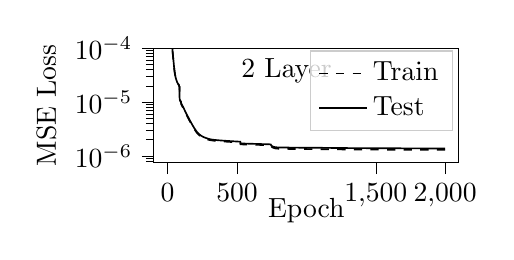
\begin{tikzpicture}

\begin{axis}[
legend cell align={left},
legend style={fill opacity=0.8, draw opacity=1, text opacity=1, draw=white!80!black},
log basis y={10},
tick align=outside,
tick pos=left,
title={2 Layer $\hy$},
title style={at={(0.45,0.85)},anchor=north},
x grid style={white!69.0196078431373!black},
xlabel={Epoch},
x label style={yshift=10pt},
xmin=-99.95, xmax=2098.95,
xtick style={color=black},
xtick = {0,500,1500,2000},
y grid style={white!69.0196078431373!black},
ylabel={MSE Loss},
ymin=7.6063321892292e-07, ymax=1e-4,
ymode=log,
ytick style={color=black},
width=.45\textwidth,
height=.25\textwidth
]
\addplot [semithick, black, dashed]
table {%
0 0.0518386695683002
1 0.042526340380311
2 0.0347423156872392
3 0.0278063397407532
4 0.021599099136889
5 0.0169535573758185
6 0.0133449736572802
7 0.0096524867080152
8 0.00607697855122387
9 0.00346671832166612
10 0.00228777943272144
11 0.00164228947134689
12 0.00122930787573569
13 0.000946592513937503
14 0.000754222130053677
15 0.000623254176578484
16 0.000526171202189289
17 0.000440977271879092
18 0.00037380238971673
19 0.000321372847538441
20 0.00028025879181223
21 0.000247563553391956
22 0.000221549878042424
23 0.000200674695734051
24 0.000183563173413859
25 0.000169053649296984
26 0.000156700562307378
27 0.000145990131146391
28 0.000136467741052911
29 0.000127828117649187
30 0.000119895841526159
31 0.000112545413488988
32 0.000105680738532101
33 9.92588357621571e-05
34 9.3258946260903e-05
35 8.76442736916943e-05
36 8.23576925613452e-05
37 7.73938517377246e-05
38 7.27130913655856e-05
39 6.8314350421133e-05
40 6.41955712490017e-05
41 6.03399962346884e-05
42 5.67417087368085e-05
43 5.33954841157538e-05
44 5.0292471962166e-05
45 4.74299892848649e-05
46 4.48063469739282e-05
47 4.24147469020681e-05
48 4.02486506536661e-05
49 3.82998454442713e-05
50 3.65582336962689e-05
51 3.50118609967467e-05
52 3.36569491373666e-05
53 3.24788894431549e-05
54 3.14478582076845e-05
55 3.05533147147798e-05
56 2.97498192085186e-05
57 2.89429238437151e-05
58 2.82225572700554e-05
59 2.75767276507395e-05
60 2.69969247092376e-05
61 2.646950968483e-05
62 2.59851477894699e-05
63 2.55374307816965e-05
64 2.51249913926586e-05
65 2.47355156570848e-05
66 2.43629243705072e-05
67 2.39832626575662e-05
68 2.35637702317035e-05
69 2.32211665752402e-05
70 2.29383413134201e-05
71 2.26900584239047e-05
72 2.24617844360182e-05
73 2.22450978726556e-05
74 2.20345916350197e-05
75 2.18275812112552e-05
76 2.16219654867018e-05
77 2.1417711785034e-05
78 2.1214236781816e-05
79 2.10117783281021e-05
80 2.08105283381883e-05
81 2.06107105623232e-05
82 2.04136253305478e-05
83 1.99121589284914e-05
84 1.94468321642489e-05
85 1.92526021455706e-05
86 1.68429254481453e-05
87 1.11265583582281e-05
88 1.08224221194178e-05
89 1.06731547539312e-05
90 1.05443111642671e-05
91 1.04219903960256e-05
92 1.03025638554755e-05
93 1.01851757890472e-05
94 1.00690036970263e-05
95 9.95377955223375e-06
96 9.83960515168292e-06
97 9.6077903663172e-06
98 9.08970189311731e-06
99 8.98518852409325e-06
100 8.88667989238456e-06
101 8.78861929595587e-06
102 8.69103235254443e-06
103 8.59354773410814e-06
104 8.49647685981836e-06
105 8.39990374788613e-06
106 8.30380843763123e-06
107 8.20817358044224e-06
108 8.11326919119892e-06
109 8.0190826447506e-06
110 7.92535356458757e-06
111 7.83217436401173e-06
112 7.73989984918444e-06
113 7.64807627137998e-06
114 7.5570470621642e-06
115 7.46617350023371e-06
116 7.37646823699834e-06
117 7.28749768268244e-06
118 7.19915332319943e-06
119 7.11171480043049e-06
120 7.0252807649922e-06
121 6.93957605744799e-06
122 6.8550750625036e-06
123 6.77161231669743e-06
124 6.68928749064435e-06
125 6.60800705782094e-06
126 6.52786106229541e-06
127 6.44881835250999e-06
128 6.3709648547956e-06
129 6.29415914409037e-06
130 6.21850223342335e-06
131 6.14401825305322e-06
132 6.07067480086698e-06
133 5.99841532675782e-06
134 5.92726610238969e-06
135 5.85724698703416e-06
136 5.78829684695847e-06
137 5.72039379244416e-06
138 5.65365198121981e-06
139 5.58796158020414e-06
140 5.52333012819872e-06
141 5.45967585458129e-06
142 5.39706647441562e-06
143 5.33535780868988e-06
144 5.27458272108561e-06
145 5.21480528050233e-06
146 5.15576177031107e-06
147 5.09760672775883e-06
148 5.04035929361635e-06
149 4.98399535490535e-06
150 4.92840583774523e-06
151 4.87364144305502e-06
152 4.81966467486927e-06
153 4.76406977395527e-06
154 4.69791715545398e-06
155 4.64507658807634e-06
156 4.59343973466275e-06
157 4.54271117132521e-06
158 4.49279561598814e-06
159 4.4436497382776e-06
160 4.39516718938648e-06
161 4.34741592334831e-06
162 4.30033761358573e-06
163 4.25400164704115e-06
164 4.20822800037968e-06
165 4.16278015359239e-06
166 4.1181904248333e-06
167 4.07423587330413e-06
168 4.0309002961294e-06
169 3.98809872649508e-06
170 3.94593327928305e-06
171 3.90432318772582e-06
172 3.86316539697873e-06
173 3.82265143798577e-06
174 3.78271101931205e-06
175 3.74335995593356e-06
176 3.70451060553023e-06
177 3.66598950404295e-06
178 3.62826339983258e-06
179 3.59102522270405e-06
180 3.55434255129694e-06
181 3.51821511981143e-06
182 3.4826161552246e-06
183 3.44756884828712e-06
184 3.41307895928367e-06
185 3.3791370713061e-06
186 3.34570067798268e-06
187 3.31284759954542e-06
188 3.28047421021438e-06
189 3.24868683401291e-06
190 3.21743388849427e-06
191 3.1866992187588e-06
192 3.15648334390062e-06
193 3.12686154870789e-06
194 3.09775542154966e-06
195 3.0692054060637e-06
196 3.04119435577377e-06
197 3.01375761148392e-06
198 2.98678445994938e-06
199 2.96039846932672e-06
200 2.93452443952447e-06
201 2.90920865177213e-06
202 2.88442320947979e-06
203 2.86015471203882e-06
204 2.83649073071501e-06
205 2.81332962913439e-06
206 2.79064786889194e-06
207 2.76854250500946e-06
208 2.74696784845219e-06
209 2.72586062430946e-06
210 2.70531269256935e-06
211 2.68526590684814e-06
212 2.66566363393395e-06
213 2.64662573533769e-06
214 2.6280339858431e-06
215 2.60993901497386e-06
216 2.59233656379365e-06
217 2.57519019442043e-06
218 2.55849347206549e-06
219 2.54225137109643e-06
220 2.52648555715496e-06
221 2.51116403057949e-06
222 2.49626635525146e-06
223 2.48174041792026e-06
224 2.46764998712479e-06
225 2.45395659851511e-06
226 2.44061466628409e-06
227 2.42766318024223e-06
228 2.41510581383864e-06
229 2.40287865153732e-06
230 2.39102976365757e-06
231 2.37946973879843e-06
232 2.36823859097512e-06
233 2.35734377997687e-06
234 2.34669803728593e-06
235 2.33637789938257e-06
236 2.32633338055166e-06
237 2.31655079858228e-06
238 2.30704811121996e-06
239 2.29775435502688e-06
240 2.28908307065012e-06
241 2.28025623937356e-06
242 2.27162592034347e-06
243 2.26319784212592e-06
244 2.2550409375981e-06
245 2.24706835138022e-06
246 2.23929092283015e-06
247 2.23166111379669e-06
248 2.22424669038901e-06
249 2.21699714541046e-06
250 2.20993513937628e-06
251 2.20302234424707e-06
252 2.19623759960541e-06
253 2.18960344636798e-06
254 2.18315790721135e-06
255 2.17678003446053e-06
256 2.17060044519712e-06
257 2.16451002290796e-06
258 2.15849525591238e-06
259 2.15263430231971e-06
260 2.14691730741379e-06
261 2.14129940786734e-06
262 2.13577006115884e-06
263 2.13036238608311e-06
264 2.12501493570016e-06
265 2.1199581875635e-06
266 2.11479780750778e-06
267 2.10963459062441e-06
268 2.10465096063217e-06
269 2.09979531643967e-06
270 2.09493869374455e-06
271 2.09029867505706e-06
272 2.08560229043542e-06
273 2.08097659026407e-06
274 2.07650576862761e-06
275 2.07193567734976e-06
276 2.06749240817317e-06
277 2.06326575550975e-06
278 2.05894802388684e-06
279 2.05470462492485e-06
280 2.05050052682054e-06
281 2.04643580877928e-06
282 2.0424704373454e-06
283 2.03852960294171e-06
284 2.03469342307017e-06
285 2.03091579976444e-06
286 2.02713633768781e-06
287 2.02345604839138e-06
288 2.01982171290638e-06
289 2.01625873410194e-06
290 2.01274700611975e-06
291 2.00929016750706e-06
292 2.00590146562263e-06
293 2.00254602100358e-06
294 1.99926750190116e-06
295 1.99598840447379e-06
296 1.99279543198827e-06
297 1.98967802123207e-06
298 1.98662693992446e-06
299 1.98363486015296e-06
300 1.98073774367913e-06
301 1.97792627022864e-06
302 1.97517233220879e-06
303 1.97249674567956e-06
304 1.96989209428011e-06
305 1.96735570136752e-06
306 1.96489110953735e-06
307 1.96252498756166e-06
308 1.96016407414845e-06
309 1.95790429916087e-06
310 1.95567747516634e-06
311 1.95353562503442e-06
312 1.95143923531305e-06
313 1.94938852894211e-06
314 1.94739756454965e-06
315 1.94547211549434e-06
316 1.94368945972201e-06
317 1.94186115868433e-06
318 1.94003258525299e-06
319 1.93824945745291e-06
320 1.9365728117009e-06
321 1.93486980356283e-06
322 1.93323022483582e-06
323 1.93159868342718e-06
324 1.93004855782419e-06
325 1.92850577320769e-06
326 1.92703124560012e-06
327 1.92557061188836e-06
328 1.92414228069993e-06
329 1.92272855258579e-06
330 1.92145235405405e-06
331 1.92011111062129e-06
332 1.91873049038804e-06
333 1.91744816731898e-06
334 1.91613417905501e-06
335 1.91486396772689e-06
336 1.91374089342844e-06
337 1.91252254262508e-06
338 1.91134569661244e-06
339 1.91014032100156e-06
340 1.90892861962766e-06
341 1.90778080786913e-06
342 1.90679503680258e-06
343 1.90562279988171e-06
344 1.90453983475436e-06
345 1.9034283604924e-06
346 1.90236943444688e-06
347 1.90128401038692e-06
348 1.90023423112962e-06
349 1.89921649234748e-06
350 1.89817762452549e-06
351 1.89717194177774e-06
352 1.89619797345131e-06
353 1.89519621744694e-06
354 1.89419035530136e-06
355 1.89321117386498e-06
356 1.89228158308197e-06
357 1.89132848026929e-06
358 1.89040515931538e-06
359 1.8894536552807e-06
360 1.88852625899472e-06
361 1.8876163518371e-06
362 1.88671577905097e-06
363 1.88581250529296e-06
364 1.88489490290067e-06
365 1.88400545243894e-06
366 1.88320691779609e-06
367 1.88227364219529e-06
368 1.88137783914044e-06
369 1.88048757183878e-06
370 1.87960764208128e-06
371 1.87875062977128e-06
372 1.87785555567643e-06
373 1.87700367860089e-06
374 1.8761265273497e-06
375 1.87530233984035e-06
376 1.87443296317724e-06
377 1.87359234882933e-06
378 1.87277639042804e-06
379 1.87191020336286e-06
380 1.87106933947234e-06
381 1.87022027148487e-06
382 1.86942492166509e-06
383 1.86859680513862e-06
384 1.86778859585957e-06
385 1.86696180901436e-06
386 1.86615413451818e-06
387 1.865346644081e-06
388 1.86454020524707e-06
389 1.86374061308925e-06
390 1.86296425601995e-06
391 1.86214191205636e-06
392 1.86135847434343e-06
393 1.86057959820118e-06
394 1.85977571720741e-06
395 1.85900325470811e-06
396 1.85821711534118e-06
397 1.85742586654669e-06
398 1.85668396852634e-06
399 1.85587053044856e-06
400 1.85511533595673e-06
401 1.85435227967901e-06
402 1.85357387726981e-06
403 1.85281492088052e-06
404 1.85205200068594e-06
405 1.85128828331926e-06
406 1.85053131349377e-06
407 1.8499851529441e-06
408 1.84917399599271e-06
409 1.84840255906238e-06
410 1.84766332199615e-06
411 1.84689625007195e-06
412 1.84613141198042e-06
413 1.84538050450556e-06
414 1.844629050197e-06
415 1.84387742933723e-06
416 1.84314657485629e-06
417 1.84239931502361e-06
418 1.84165844211748e-06
419 1.84091300036471e-06
420 1.84018742834269e-06
421 1.83944933723978e-06
422 1.83872336367585e-06
423 1.83799873639146e-06
424 1.83724605551561e-06
425 1.83653046701693e-06
426 1.83579679980994e-06
427 1.83508214388439e-06
428 1.83435587473468e-06
429 1.83363736755382e-06
430 1.8329269255446e-06
431 1.83219673760959e-06
432 1.83147712380105e-06
433 1.83076220457679e-06
434 1.83004805330711e-06
435 1.82932657037327e-06
436 1.82861742405294e-06
437 1.82790977305558e-06
438 1.82720573548067e-06
439 1.82647991425711e-06
440 1.82577657187721e-06
441 1.82505562622737e-06
442 1.82437355033471e-06
443 1.82366404123968e-06
444 1.82293964576274e-06
445 1.82224642969686e-06
446 1.82155447021159e-06
447 1.82083569222868e-06
448 1.82014943925424e-06
449 1.81945615088352e-06
450 1.81874204338328e-06
451 1.81806114380834e-06
452 1.8173547899778e-06
453 1.81667541403385e-06
454 1.81598416770612e-06
455 1.81524100480601e-06
456 1.81453961306488e-06
457 1.81385451594451e-06
458 1.81315790109693e-06
459 1.81245884846248e-06
460 1.81177978004143e-06
461 1.81107571381744e-06
462 1.81042428357614e-06
463 1.80971381985273e-06
464 1.80901504791109e-06
465 1.80835478647623e-06
466 1.80766282676359e-06
467 1.80698605220186e-06
468 1.80630960915096e-06
469 1.80562094067227e-06
470 1.80495204324416e-06
471 1.80429276622363e-06
472 1.80363471463352e-06
473 1.80292723803177e-06
474 1.80225790609256e-06
475 1.80158976775147e-06
476 1.80091279730732e-06
477 1.80023987002187e-06
478 1.79959257354767e-06
479 1.79890977392461e-06
480 1.79824207714319e-06
481 1.79757481157594e-06
482 1.7969080555531e-06
483 1.79623438566523e-06
484 1.79557559511068e-06
485 1.79491270898779e-06
486 1.79438170130197e-06
487 1.79366591225971e-06
488 1.79298442958498e-06
489 1.79231373408584e-06
490 1.79167655073798e-06
491 1.79100179059333e-06
492 1.79032596940942e-06
493 1.78968522516243e-06
494 1.78901104857232e-06
495 1.78837366763673e-06
496 1.78771149103341e-06
497 1.78705672965407e-06
498 1.78641258935386e-06
499 1.78577213569042e-06
500 1.78510025034484e-06
501 1.78445535595984e-06
502 1.78384143919175e-06
503 1.78316099584208e-06
504 1.7825342940796e-06
505 1.78187944834463e-06
506 1.78124007402403e-06
507 1.78060222037857e-06
508 1.77995303192802e-06
509 1.77932496455924e-06
510 1.77868458877128e-06
511 1.77803215694894e-06
512 1.77739755554285e-06
513 1.77675821737466e-06
514 1.77612358766055e-06
515 1.77547155703905e-06
516 1.77483872244011e-06
517 1.77422070601096e-06
518 1.7735807008421e-06
519 1.77294365573744e-06
520 1.77230281133234e-06
521 1.77169832647905e-06
522 1.77105510329056e-06
523 1.77042892869395e-06
524 1.76978312288156e-06
525 1.66620164694109e-06
526 1.63933637233526e-06
527 1.63880179010789e-06
528 1.63844974755989e-06
529 1.63812484262849e-06
530 1.63779529955832e-06
531 1.63742095688235e-06
532 1.63711894725793e-06
533 1.63679492797542e-06
534 1.63647552042789e-06
535 1.6361367341915e-06
536 1.63582143278518e-06
537 1.63551573919563e-06
538 1.63520860402855e-06
539 1.63490383059184e-06
540 1.63459672538124e-06
541 1.63429267476545e-06
542 1.63399191654889e-06
543 1.63368553430132e-06
544 1.63338495767107e-06
545 1.63310262541927e-06
546 1.6327682387498e-06
547 1.63247037161796e-06
548 1.63218582176228e-06
549 1.63187798207787e-06
550 1.6315871942254e-06
551 1.63128337254648e-06
552 1.63099369069641e-06
553 1.63070029680057e-06
554 1.63040730399189e-06
555 1.63011679620695e-06
556 1.62983160720387e-06
557 1.62952682003947e-06
558 1.62922214192918e-06
559 1.62894504913425e-06
560 1.62864188482104e-06
561 1.6283534936008e-06
562 1.6280654233185e-06
563 1.62778253840656e-06
564 1.62747459560819e-06
565 1.62719646951359e-06
566 1.62692239271678e-06
567 1.62661389299501e-06
568 1.62633292706005e-06
569 1.62606319807423e-06
570 1.62576276485993e-06
571 1.62547591571638e-06
572 1.62518481394613e-06
573 1.62490155244654e-06
574 1.62461253736979e-06
575 1.62433828410258e-06
576 1.62405268940802e-06
577 1.62376205736336e-06
578 1.62348133056867e-06
579 1.62319527444765e-06
580 1.62290394715114e-06
581 1.62262100627686e-06
582 1.62234837728192e-06
583 1.62206169241585e-06
584 1.6217815277173e-06
585 1.62149699008296e-06
586 1.62121524058989e-06
587 1.62092517706469e-06
588 1.62070420867622e-06
589 1.62038921615704e-06
590 1.62008199799857e-06
591 1.61979725899641e-06
592 1.61950673955857e-06
593 1.61922272562265e-06
594 1.6189295055824e-06
595 1.61864341677642e-06
596 1.61835239086372e-06
597 1.61807546018622e-06
598 1.61779094619874e-06
599 1.61749259794419e-06
600 1.61723098355537e-06
601 1.61693797414841e-06
602 1.61665728629146e-06
603 1.61636831695944e-06
604 1.61610073524798e-06
605 1.61582153997131e-06
606 1.61554774945216e-06
607 1.61525743881441e-06
608 1.61498842523145e-06
609 1.61470044996292e-06
610 1.61442914523491e-06
611 1.61414135411064e-06
612 1.61386748200698e-06
613 1.61359336857458e-06
614 1.61332622727173e-06
615 1.61304242104166e-06
616 1.61276320352499e-06
617 1.61248982448114e-06
618 1.61219475916141e-06
619 1.61193266151827e-06
620 1.61164703547456e-06
621 1.61138146705753e-06
622 1.61109890345301e-06
623 1.61082260021317e-06
624 1.61053988405513e-06
625 1.61026904530104e-06
626 1.6099991666465e-06
627 1.60971038680202e-06
628 1.60944881005776e-06
629 1.60917611752609e-06
630 1.60890855008233e-06
631 1.60862766114178e-06
632 1.60834999020665e-06
633 1.60807368021665e-06
634 1.60779430278524e-06
635 1.60753966724769e-06
636 1.60726439040104e-06
637 1.60700710711126e-06
638 1.60672452217625e-06
639 1.60644054170689e-06
640 1.60616960967275e-06
641 1.60589141702872e-06
642 1.60563484433851e-06
643 1.6053435355019e-06
644 1.60508566412432e-06
645 1.60482664446704e-06
646 1.60453707941599e-06
647 1.6042754193677e-06
648 1.60399306275849e-06
649 1.60374430119248e-06
650 1.6034647498202e-06
651 1.60318650912927e-06
652 1.60291618941244e-06
653 1.60264964672763e-06
654 1.60237670334595e-06
655 1.60212423365635e-06
656 1.60184172608524e-06
657 1.60158811885935e-06
658 1.60129746804216e-06
659 1.60103951819224e-06
660 1.60076912700902e-06
661 1.60050588327465e-06
662 1.60023428719569e-06
663 1.59996088962089e-06
664 1.59969389768833e-06
665 1.59941708385247e-06
666 1.59916993624165e-06
667 1.59889477750141e-06
668 1.59866888432703e-06
669 1.59837924398687e-06
670 1.59808459493149e-06
671 1.59782723729052e-06
672 1.5975413056708e-06
673 1.59727512193797e-06
674 1.59698751379267e-06
675 1.59672256081933e-06
676 1.59644536088877e-06
677 1.59617859861783e-06
678 1.59590370850538e-06
679 1.59562858524964e-06
680 1.59536997378495e-06
681 1.59507531752467e-06
682 1.59482622048301e-06
683 1.59457645222005e-06
684 1.59428069426326e-06
685 1.5940048189691e-06
686 1.59374665537371e-06
687 1.59347681504585e-06
688 1.59320771297189e-06
689 1.59294189681702e-06
690 1.59265840376577e-06
691 1.59240391452897e-06
692 1.59212388167873e-06
693 1.59185475271784e-06
694 1.59160081452114e-06
695 1.5913355798034e-06
696 1.59105049479535e-06
697 1.59078170094062e-06
698 1.5905177025104e-06
699 1.59024808239394e-06
700 1.5899925537326e-06
701 1.58970312894269e-06
702 1.58944773028225e-06
703 1.58917952906279e-06
704 1.58889819385877e-06
705 1.5886472953639e-06
706 1.58836964335762e-06
707 1.58811646971913e-06
708 1.58783535489704e-06
709 1.58757957046873e-06
710 1.58731703973558e-06
711 1.58704471705562e-06
712 1.58677873791646e-06
713 1.5865028876334e-06
714 1.58624447136901e-06
715 1.58597577814135e-06
716 1.58570803385771e-06
717 1.58545115763786e-06
718 1.58517122966373e-06
719 1.58490910264675e-06
720 1.58464107597922e-06
721 1.58438146414142e-06
722 1.58410357899186e-06
723 1.58384261210642e-06
724 1.58350118182682e-06
725 1.58321730540933e-06
726 1.58293486397554e-06
727 1.58265849421468e-06
728 1.58239726721376e-06
729 1.58211539564945e-06
730 1.58183252307253e-06
731 1.58156696035405e-06
732 1.58106459616647e-06
733 1.5807887297683e-06
734 1.580489066626e-06
735 1.58021400281427e-06
736 1.57994096404934e-06
737 1.57964867177895e-06
738 1.57935908634954e-06
739 1.57908623067726e-06
740 1.57895105029127e-06
741 1.57861684205329e-06
742 1.57829686450839e-06
743 1.57820503723372e-06
744 1.56886491616604e-06
745 1.54443650944813e-06
746 1.52464937485774e-06
747 1.5084941576049e-06
748 1.49567416087848e-06
749 1.48492991016269e-06
750 1.47589340608079e-06
751 1.46807804819105e-06
752 1.46103214052573e-06
753 1.45476694632407e-06
754 1.44896854914123e-06
755 1.44370241736169e-06
756 1.43866883598776e-06
757 1.43380883416455e-06
758 1.42928160187239e-06
759 1.42504067417804e-06
760 1.42097017825904e-06
761 1.41716485458687e-06
762 1.41355964707657e-06
763 1.41026495602148e-06
764 1.40694243066264e-06
765 1.40386480411792e-06
766 1.40090109704261e-06
767 1.39811546335977e-06
768 1.39556718215772e-06
769 1.39314711935867e-06
770 1.39085914671e-06
771 1.38873771130932e-06
772 1.38676904158785e-06
773 1.38486147091044e-06
774 1.38307318255215e-06
775 1.38140495923267e-06
776 1.37981144834498e-06
777 1.37832817009098e-06
778 1.37694258201293e-06
779 1.37560938435399e-06
780 1.3743737128209e-06
781 1.3732237981543e-06
782 1.3721374578779e-06
783 1.37116235606527e-06
784 1.37018989329363e-06
785 1.36925985286496e-06
786 1.36841710016711e-06
787 1.36757084865735e-06
788 1.36681302183206e-06
789 1.36608643293812e-06
790 1.36541132677337e-06
791 1.36474158155409e-06
792 1.36417904980135e-06
793 1.36355554245426e-06
794 1.36299955610752e-06
795 1.36246179810939e-06
796 1.36196002624445e-06
797 1.36147286586663e-06
798 1.36102072210065e-06
799 1.36058262586403e-06
800 1.36019539741028e-06
801 1.35977008343957e-06
802 1.35934900353618e-06
803 1.35907496527921e-06
804 1.35871082459005e-06
805 1.35838341267913e-06
806 1.35806158336038e-06
807 1.35770684502745e-06
808 1.35738369530713e-06
809 1.35709290060504e-06
810 1.35672559207478e-06
811 1.35645564012066e-06
812 1.35619012348798e-06
813 1.35594104767733e-06
814 1.35568918759077e-06
815 1.35547467380093e-06
816 1.35525254742674e-06
817 1.35503257631342e-06
818 1.35482675494814e-06
819 1.35461341591281e-06
820 1.35443167101812e-06
821 1.35425345231965e-06
822 1.3540686281317e-06
823 1.35388498344469e-06
824 1.35370961773162e-06
825 1.35353743995381e-06
826 1.3533792219107e-06
827 1.35313768534218e-06
828 1.35298258597061e-06
829 1.352827967807e-06
830 1.3526768412504e-06
831 1.35252841401723e-06
832 1.35240225704081e-06
833 1.35225109995929e-06
834 1.35212322014411e-06
835 1.35198998505359e-06
836 1.35184609810324e-06
837 1.35173012962753e-06
838 1.35159571098598e-06
839 1.35147283796755e-06
840 1.35134105134682e-06
841 1.35123280175264e-06
842 1.35110112422865e-06
843 1.35098620997098e-06
844 1.3508639218287e-06
845 1.35077587185606e-06
846 1.35064492155834e-06
847 1.35053679737496e-06
848 1.35042975225019e-06
849 1.35031924180851e-06
850 1.35021662519819e-06
851 1.35011604727708e-06
852 1.35000363111715e-06
853 1.34990536004409e-06
854 1.3498181129421e-06
855 1.34971324047228e-06
856 1.34960946446938e-06
857 1.34950742594242e-06
858 1.34941408889233e-06
859 1.34932775988261e-06
860 1.34922658703829e-06
861 1.34912472361748e-06
862 1.34902612357735e-06
863 1.34892750345728e-06
864 1.34883547387687e-06
865 1.34874449845768e-06
866 1.34864384494904e-06
867 1.34856915693149e-06
868 1.348471884981e-06
869 1.34839657053476e-06
870 1.34830537385255e-06
871 1.34821930835471e-06
872 1.34813692710622e-06
873 1.34803793085325e-06
874 1.34795173156022e-06
875 1.3478776119058e-06
876 1.34777355222582e-06
877 1.34769706210136e-06
878 1.34761042174603e-06
879 1.34751966670876e-06
880 1.34744346894422e-06
881 1.34735287390697e-06
882 1.34725689983384e-06
883 1.34717631696901e-06
884 1.34709783374376e-06
885 1.34702141804155e-06
886 1.34693583878231e-06
887 1.34685476582774e-06
888 1.34676708303516e-06
889 1.34668838386176e-06
890 1.3466111598035e-06
891 1.34654315939997e-06
892 1.34647579018576e-06
893 1.34638291420686e-06
894 1.34629611308412e-06
895 1.34621114347055e-06
896 1.34613849976972e-06
897 1.34607026022593e-06
898 1.34600097389637e-06
899 1.34590469681939e-06
900 1.34583183752568e-06
901 1.3457547924105e-06
902 1.34568102149046e-06
903 1.34570885896323e-06
904 1.34563602135529e-06
905 1.34554965568157e-06
906 1.34547586169731e-06
907 1.34539394407795e-06
908 1.34532783863506e-06
909 1.34524034038463e-06
910 1.34516967027309e-06
911 1.34509670238003e-06
912 1.34502306164563e-06
913 1.34495103804966e-06
914 1.34488076425043e-06
915 1.34479510651886e-06
916 1.34472651404849e-06
917 1.34466214339568e-06
918 1.34458127747905e-06
919 1.34450533219876e-06
920 1.3444267981555e-06
921 1.34435084679296e-06
922 1.34428695463384e-06
923 1.34422671932555e-06
924 1.34414231379765e-06
925 1.34407956909399e-06
926 1.3439992275579e-06
927 1.3439298076463e-06
928 1.34387832962091e-06
929 1.3438092536262e-06
930 1.34373289975542e-06
931 1.3436577213497e-06
932 1.34358143714053e-06
933 1.34352394559301e-06
934 1.34345717660267e-06
935 1.34337900578885e-06
936 1.34335605609692e-06
937 1.34328150070928e-06
938 1.34321433966988e-06
939 1.34313157009558e-06
940 1.3430716178533e-06
941 1.34299877356625e-06
942 1.3429399402014e-06
943 1.34285865880202e-06
944 1.34280206063409e-06
945 1.34274019325176e-06
946 1.34266461981269e-06
947 1.34259506944545e-06
948 1.34254850138404e-06
949 1.34247986547109e-06
950 1.34240087921e-06
951 1.34232612865048e-06
952 1.3423135030024e-06
953 1.34225830529999e-06
954 1.3421897558743e-06
955 1.34212832678315e-06
956 1.34206213189714e-06
957 1.34198343585012e-06
958 1.34193174501718e-06
959 1.34187326334256e-06
960 1.34180413468243e-06
961 1.34174007241938e-06
962 1.34166821864312e-06
963 1.34160912554648e-06
964 1.34154919388152e-06
965 1.34148838895953e-06
966 1.34141044561886e-06
967 1.34135855292072e-06
968 1.34130112543573e-06
969 1.34123174636613e-06
970 1.34118099316538e-06
971 1.34110277215882e-06
972 1.34103400789343e-06
973 1.34098474899247e-06
974 1.34092078039316e-06
975 1.34086393288158e-06
976 1.34079251927233e-06
977 1.34072488621939e-06
978 1.34067154296247e-06
979 1.34060519832246e-06
980 1.34055623038876e-06
981 1.34048152499133e-06
982 1.3404323760966e-06
983 1.34035964379109e-06
984 1.34030211174263e-06
985 1.34024774162356e-06
986 1.34017881156012e-06
987 1.3401354625131e-06
988 1.34007251983803e-06
989 1.34001645538717e-06
990 1.33994008200489e-06
991 1.33989448013949e-06
992 1.33979940444817e-06
993 1.3397541583231e-06
994 1.33968041419052e-06
995 1.33962406884791e-06
996 1.33956490974185e-06
997 1.33950567945362e-06
998 1.33946297422938e-06
999 1.33938883983831e-06
1000 1.33933092904215e-06
1001 1.33928694378937e-06
1002 1.33921256117731e-06
1003 1.33916161001935e-06
1004 1.3390988379598e-06
1005 1.33903752758613e-06
1006 1.33898176045477e-06
1007 1.33892504666733e-06
1008 1.33887592123472e-06
1009 1.33881134048863e-06
1010 1.33875219198387e-06
1011 1.33870028915339e-06
1012 1.33863348575858e-06
1013 1.33858250521257e-06
1014 1.33852591613959e-06
1015 1.33846663027271e-06
1016 1.33840421788989e-06
1017 1.33835072642796e-06
1018 1.33830789980038e-06
1019 1.33824401744675e-06
1020 1.33817713299322e-06
1021 1.33813398639404e-06
1022 1.33806409412784e-06
1023 1.33800658908001e-06
1024 1.33795149331206e-06
1025 1.3379155276283e-06
1026 1.33784969801809e-06
1027 1.33778447249711e-06
1028 1.33765031387156e-06
1029 1.33759461118643e-06
1030 1.33753808258064e-06
1031 1.33748855502347e-06
1032 1.33742270143955e-06
1033 1.33736784084704e-06
1034 1.33731045195873e-06
1035 1.33725952910879e-06
1036 1.33719250703734e-06
1037 1.33714265534479e-06
1038 1.33709573304941e-06
1039 1.33703461840184e-06
1040 1.33698563801943e-06
1041 1.33692117942985e-06
1042 1.33686207065864e-06
1043 1.33682150280379e-06
1044 1.33675993406257e-06
1045 1.33670628150639e-06
1046 1.33664372732767e-06
1047 1.33658942088744e-06
1048 1.33653863915129e-06
1049 1.33648365992656e-06
1050 1.33643210853052e-06
1051 1.33637117450292e-06
1052 1.33631502657749e-06
1053 1.33626177149893e-06
1054 1.33622257948218e-06
1055 1.33616662400016e-06
1056 1.33610955839458e-06
1057 1.33605329271802e-06
1058 1.33598385832556e-06
1059 1.33594217295752e-06
1060 1.33588493156367e-06
1061 1.33583359792055e-06
1062 1.33576979409611e-06
1063 1.33572435426288e-06
1064 1.33567137682178e-06
1065 1.33562173462565e-06
1066 1.33556964851778e-06
1067 1.33551589878778e-06
1068 1.33546273754348e-06
1069 1.33540153122169e-06
1070 1.33536268666035e-06
1071 1.33529603027682e-06
1072 1.33524601922375e-06
1073 1.33519661385151e-06
1074 1.33514066943974e-06
1075 1.33509146333211e-06
1076 1.33504329576795e-06
1077 1.33499757205868e-06
1078 1.33493545313001e-06
1079 1.33489117727947e-06
1080 1.33483645198851e-06
1081 1.33478451633096e-06
1082 1.33473267716511e-06
1083 1.33466724497566e-06
1084 1.33462421723607e-06
1085 1.33456596925896e-06
1086 1.33453018727892e-06
1087 1.33446277706639e-06
1088 1.33441716130278e-06
1089 1.33436078276361e-06
1090 1.33430692164893e-06
1091 1.33425975168677e-06
1092 1.33421545604051e-06
1093 1.33415072625098e-06
1094 1.33410108566068e-06
1095 1.33404680869376e-06
1096 1.33399491723196e-06
1097 1.33394408973686e-06
1098 1.33389038987275e-06
1099 1.33383919941821e-06
1100 1.33379414305068e-06
1101 1.33373261306247e-06
1102 1.33368463527006e-06
1103 1.33363207953607e-06
1104 1.33359130424537e-06
1105 1.33354491660498e-06
1106 1.33348266453481e-06
1107 1.33343180641532e-06
1108 1.33338205131395e-06
1109 1.33333231407562e-06
1110 1.33328824017553e-06
1111 1.33323012887843e-06
1112 1.33317537382993e-06
1113 1.33314741407276e-06
1114 1.33307755031353e-06
1115 1.33303352079395e-06
1116 1.33297956337231e-06
1117 1.3329289483579e-06
1118 1.33287542442417e-06
1119 1.33282477237628e-06
1120 1.33277926930475e-06
1121 1.33273204622242e-06
1122 1.33267181597319e-06
1123 1.332627589818e-06
1124 1.33257524055352e-06
1125 1.33252936851136e-06
1126 1.33248547196274e-06
1127 1.33243876933875e-06
1128 1.33238333026497e-06
1129 1.33232479907974e-06
1130 1.33227799227598e-06
1131 1.33223086616852e-06
1132 1.33218174798344e-06
1133 1.33213632797435e-06
1134 1.33208051036604e-06
1135 1.33205012393489e-06
1136 1.33198282409808e-06
1137 1.33193860241931e-06
1138 1.33188387665939e-06
1139 1.33183967609796e-06
1140 1.33179460509325e-06
1141 1.33174281238269e-06
1142 1.33169365426511e-06
1143 1.33164133212915e-06
1144 1.33158321374083e-06
1145 1.3315432472325e-06
1146 1.33148943393735e-06
1147 1.33144728846446e-06
1148 1.33139592961129e-06
1149 1.33134038986782e-06
1150 1.33129153603306e-06
1151 1.33124128893769e-06
1152 1.3311990425251e-06
1153 1.33114998108397e-06
1154 1.33109154313615e-06
1155 1.33104795212091e-06
1156 1.33099706505391e-06
1157 1.33095313810827e-06
1158 1.33090183919649e-06
1159 1.3308592359067e-06
1160 1.33080201646862e-06
1161 1.33075989552367e-06
1162 1.33070932677981e-06
1163 1.33065972174506e-06
1164 1.3306096723511e-06
1165 1.33056723711888e-06
1166 1.33051543905083e-06
1167 1.33045599883985e-06
1168 1.33043390209764e-06
1169 1.33039126671974e-06
1170 1.33034304828072e-06
1171 1.33029533026274e-06
1172 1.33023865356563e-06
1173 1.33019446022331e-06
1174 1.33014583248325e-06
1175 1.33009934955908e-06
1176 1.33004679793203e-06
1177 1.32999394267586e-06
1178 1.32859383582229e-06
1179 1.32577590167671e-06
1180 1.32481529779227e-06
1181 1.32425906130607e-06
1182 1.32385161771253e-06
1183 1.32355970555409e-06
1184 1.32332581735284e-06
1185 1.32313855300481e-06
1186 1.32299621942877e-06
1187 1.32287166445622e-06
1188 1.32275965106032e-06
1189 1.32266207796761e-06
1190 1.32258898742066e-06
1191 1.32251438074604e-06
1192 1.3224399087477e-06
1193 1.32236959144905e-06
1194 1.32232037235269e-06
1195 1.32225536714259e-06
1196 1.32219561778868e-06
1197 1.32214652194307e-06
1198 1.32208095470787e-06
1199 1.32204806527625e-06
1200 1.32199041914305e-06
1201 1.32194223348847e-06
1202 1.32188372917597e-06
1203 1.32185073353241e-06
1204 1.32179744296934e-06
1205 1.3217571945745e-06
1206 1.32170356749839e-06
1207 1.32168178934933e-06
1208 1.32160852400887e-06
1209 1.32156865880972e-06
1210 1.3215270177227e-06
1211 1.32148737561977e-06
1212 1.32144626445552e-06
1213 1.32139509810258e-06
1214 1.32141864840207e-06
1215 1.32135991154314e-06
1216 1.32131602497054e-06
1217 1.32127464453902e-06
1218 1.32121060731549e-06
1219 1.32116699967355e-06
1220 1.3211242721809e-06
1221 1.32107436284912e-06
1222 1.32103417314511e-06
1223 1.32099427466414e-06
1224 1.32095226790341e-06
1225 1.32089809829949e-06
1226 1.32086301134393e-06
1227 1.32081426257002e-06
1228 1.3207805423292e-06
1229 1.3207305637053e-06
1230 1.32068811232955e-06
1231 1.32064384796138e-06
1232 1.32060167554471e-06
1233 1.3205631688038e-06
1234 1.3205066439923e-06
1235 1.32047018907144e-06
1236 1.32054637529677e-06
1237 1.3205274783985e-06
1238 1.32047940205382e-06
1239 1.32043280677863e-06
1240 1.32039506168269e-06
1241 1.32036514655454e-06
1242 1.32031703172686e-06
1243 1.32027795616807e-06
1244 1.3202443684861e-06
1245 1.32019133667427e-06
1246 1.32015820261699e-06
1247 1.32011709712287e-06
1248 1.32007585411031e-06
1249 1.32003833635963e-06
1250 1.31999951743467e-06
1251 1.31995052718992e-06
1252 1.31991537205067e-06
1253 1.31987489763219e-06
1254 1.31983271600689e-06
1255 1.31978467074134e-06
1256 1.319753576837e-06
1257 1.31970657953673e-06
1258 1.31966508058667e-06
1259 1.319630016269e-06
1260 1.31958882650451e-06
1261 1.31953997157552e-06
1262 1.31951191637825e-06
1263 1.31946960593154e-06
1264 1.31942758504522e-06
1265 1.31938184219393e-06
1266 1.31933255261174e-06
1267 1.31929545118226e-06
1268 1.31925781937525e-06
1269 1.31922233245518e-06
1270 1.31924204031009e-06
1271 1.31918251739194e-06
1272 1.31914621874785e-06
1273 1.31909760800397e-06
1274 1.31904689864371e-06
1275 1.31899939506752e-06
1276 1.31895242788005e-06
1277 1.31888589362461e-06
1278 1.3188213102211e-06
1279 1.31876878970161e-06
1280 1.31870717576987e-06
1281 1.31865774105222e-06
1282 1.31860239366688e-06
1283 1.31855959794791e-06
1284 1.31852673801802e-06
1285 1.31848573423099e-06
1286 1.31843639238127e-06
1287 1.31837194871309e-06
1288 1.31832015325983e-06
1289 1.31827320812761e-06
1290 1.31821452710312e-06
1291 1.31826412868463e-06
1292 1.31820652498504e-06
1293 1.31813436787809e-06
1294 1.31808043758497e-06
1295 1.31803203781544e-06
1296 1.31797565646252e-06
1297 1.31792156848576e-06
1298 1.31787510680681e-06
1299 1.31782350318588e-06
1300 1.31777007236167e-06
1301 1.317731111385e-06
1302 1.31768447428726e-06
1303 1.31765222302249e-06
1304 1.31759061208925e-06
1305 1.3175407495396e-06
1306 1.31750282601217e-06
1307 1.31745717092713e-06
1308 1.31740909702671e-06
1309 1.31737010387667e-06
1310 1.31731581387839e-06
1311 1.31729359902977e-06
1312 1.31723423439212e-06
1313 1.31719637688832e-06
1314 1.31714781051073e-06
1315 1.31711109040111e-06
1316 1.31705777398849e-06
1317 1.31702496820196e-06
1318 1.31698145554537e-06
1319 1.31693504215491e-06
1320 1.316892996158e-06
1321 1.31685051350416e-06
1322 1.3168058811317e-06
1323 1.31676369285572e-06
1324 1.3167272482093e-06
1325 1.31667373887012e-06
1326 1.31663302317975e-06
1327 1.31659156795649e-06
1328 1.31655225268901e-06
1329 1.31651966761126e-06
1330 1.31647060948126e-06
1331 1.31643030140083e-06
1332 1.31639117168447e-06
1333 1.31633731963632e-06
1334 1.31630387018333e-06
1335 1.31626258671247e-06
1336 1.31621279176386e-06
1337 1.31617875889845e-06
1338 1.31613359954486e-06
1339 1.31608632344182e-06
1340 1.31604712120748e-06
1341 1.31601232321543e-06
1342 1.3159628022521e-06
1343 1.31592109164558e-06
1344 1.31588097301005e-06
1345 1.31584353617598e-06
1346 1.3158043823438e-06
1347 1.31577746958556e-06
1348 1.31573951045993e-06
1349 1.31568544951222e-06
1350 1.31564648904714e-06
1351 1.31560409097631e-06
1352 1.31556468213034e-06
1353 1.31551994411439e-06
1354 1.31547720894787e-06
1355 1.31544238529102e-06
1356 1.31539883138032e-06
1357 1.3153504088308e-06
1358 1.31530955987103e-06
1359 1.31526198380527e-06
1360 1.31523578205872e-06
1361 1.3151850012747e-06
1362 1.31514612101569e-06
1363 1.31510655799616e-06
1364 1.31506297603323e-06
1365 1.31502549686502e-06
1366 1.31497581915596e-06
1367 1.31494573567181e-06
1368 1.31489326294343e-06
1369 1.31486664048452e-06
1370 1.31481228511632e-06
1371 1.31477881735975e-06
1372 1.31473155177275e-06
1373 1.31468939930812e-06
1374 1.31464601584241e-06
1375 1.31461001865318e-06
1376 1.31457059183049e-06
1377 1.31452871148952e-06
1378 1.31448866785888e-06
1379 1.31444212428278e-06
1380 1.31440802965699e-06
1381 1.31436307299282e-06
1382 1.31431838971707e-06
1383 1.31427322443756e-06
1384 1.31423886649884e-06
1385 1.31420234399116e-06
1386 1.31415619608788e-06
1387 1.31413195184393e-06
1388 1.31408533862043e-06
1389 1.3140527643003e-06
1390 1.3140024599636e-06
1391 1.31395506453202e-06
1392 1.31391883945753e-06
1393 1.31387949465989e-06
1394 1.31384093273823e-06
1395 1.31380773196099e-06
1396 1.31375993719018e-06
1397 1.31372225746418e-06
1398 1.31367593549214e-06
1399 1.31363591665945e-06
1400 1.31359878579929e-06
1401 1.31356280685679e-06
1402 1.31351572737515e-06
1403 1.31348148261168e-06
1404 1.31343552995133e-06
1405 1.31340653955192e-06
1406 1.31335477141192e-06
1407 1.31331217909292e-06
1408 1.31328199159952e-06
1409 1.31324050759929e-06
1410 1.313199410518e-06
1411 1.31315960558709e-06
1412 1.31310952575348e-06
1413 1.31307809232339e-06
1414 1.31303962449181e-06
1415 1.3129952787807e-06
1416 1.31295043550494e-06
1417 1.31291564053981e-06
1418 1.31287857932705e-06
1419 1.31284263386533e-06
1420 1.31279429353981e-06
1421 1.31275722567636e-06
1422 1.31273118608988e-06
1423 1.31268142855845e-06
1424 1.3126316385268e-06
1425 1.31259607421441e-06
1426 1.31256069056462e-06
1427 1.31251248853914e-06
1428 1.31246915155714e-06
1429 1.31243717203233e-06
1430 1.31239350761803e-06
1431 1.31234716056383e-06
1432 1.3123242802493e-06
1433 1.31227735960238e-06
1434 1.31223271989711e-06
1435 1.31219915439829e-06
1436 1.31215062850742e-06
1437 1.31212218929022e-06
1438 1.3120791121537e-06
1439 1.31203161237181e-06
1440 1.31200182872249e-06
1441 1.31196549817503e-06
1442 1.31192107697586e-06
1443 1.31187962790591e-06
1444 1.31183938752599e-06
1445 1.31180776863005e-06
1446 1.31176054296134e-06
1447 1.31172362119969e-06
1448 1.31168643122237e-06
1449 1.31165350231299e-06
1450 1.31160334724711e-06
1451 1.3115657474998e-06
1452 1.311524503123e-06
1453 1.31148720245733e-06
1454 1.31145775291941e-06
1455 1.31141236701637e-06
1456 1.31137372878243e-06
1457 1.31133921740911e-06
1458 1.31128970619443e-06
1459 1.31125061385262e-06
1460 1.31120704479315e-06
1461 1.31118090965288e-06
1462 1.31113069129185e-06
1463 1.31109799757212e-06
1464 1.31105958655553e-06
1465 1.31102414700024e-06
1466 1.31113465407395e-06
1467 1.3115353781501e-06
1468 1.31073669899706e-06
1469 1.31061095918028e-06
1470 1.31053976475926e-06
1471 1.31051849380981e-06
1472 1.31045500958749e-06
1473 1.31041446591951e-06
1474 1.31038325683619e-06
1475 1.31034178316725e-06
1476 1.31030691308354e-06
1477 1.31025875219848e-06
1478 1.31020995374342e-06
1479 1.31017023034019e-06
1480 1.31014068551849e-06
1481 1.31009896698231e-06
1482 1.31005129526329e-06
1483 1.31001381359397e-06
1484 1.30997352819406e-06
1485 1.30993995983886e-06
1486 1.30989869869325e-06
1487 1.30986009870071e-06
1488 1.30982312171568e-06
1489 1.30978367678836e-06
1490 1.30974461123401e-06
1491 1.30970787867568e-06
1492 1.30966502571539e-06
1493 1.3096298849149e-06
1494 1.30959659510665e-06
1495 1.30956331126697e-06
1496 1.30951565556359e-06
1497 1.3094790621011e-06
1498 1.30944215527506e-06
1499 1.30939618007631e-06
1500 1.30936962753481e-06
1501 1.30933061875282e-06
1502 1.30928901221239e-06
1503 1.30924293445389e-06
1504 1.30921448861443e-06
1505 1.30917329974523e-06
1506 1.3091434063881e-06
1507 1.3091095128317e-06
1508 1.30906401409447e-06
1509 1.30902855379134e-06
1510 1.30899295051279e-06
1511 1.30895525619223e-06
1512 1.30891014282497e-06
1513 1.30888283999298e-06
1514 1.30883949670135e-06
1515 1.30880467609984e-06
1516 1.30876093874122e-06
1517 1.30873182040148e-06
1518 1.30869287713153e-06
1519 1.30865213854747e-06
1520 1.30861667719273e-06
1521 1.3085740121852e-06
1522 1.30854242374312e-06
1523 1.30850691304829e-06
1524 1.30846172521615e-06
1525 1.3084308924789e-06
1526 1.30839026867591e-06
1527 1.30835211136571e-06
1528 1.30831085695604e-06
1529 1.30828064069988e-06
1530 1.308229396912e-06
1531 1.3081966038726e-06
1532 1.30816021432167e-06
1533 1.30811588522306e-06
1534 1.30807387886023e-06
1535 1.30804364836479e-06
1536 1.30800523677976e-06
1537 1.3079673543217e-06
1538 1.30793483285174e-06
1539 1.30789522229691e-06
1540 1.30785042148318e-06
1541 1.30781459185414e-06
1542 1.30778182165159e-06
1543 1.30775194134003e-06
1544 1.30771855249634e-06
1545 1.30767076348093e-06
1546 1.30763190119865e-06
1547 1.30759709659856e-06
1548 1.30755398699023e-06
1549 1.30752424855984e-06
1550 1.30748375099188e-06
1551 1.30745104392815e-06
1552 1.30741234369225e-06
1553 1.30737575641149e-06
1554 1.30733214440681e-06
1555 1.30730984595573e-06
1556 1.3072714322675e-06
1557 1.30723216413742e-06
1558 1.30718758191506e-06
1559 1.307162111857e-06
1560 1.3071203532462e-06
1561 1.30709440516341e-06
1562 1.30705507541506e-06
1563 1.30701736974004e-06
1564 1.30697946784153e-06
1565 1.30694769262618e-06
1566 1.30688747393037e-06
1567 1.30680106401826e-06
1568 1.30671250040848e-06
1569 1.30658519580606e-06
1570 1.30647350641766e-06
1571 1.30637264372524e-06
1572 1.30628260801302e-06
1573 1.30619263643439e-06
1574 1.30612632679572e-06
1575 1.3060445271833e-06
1576 1.30598045691954e-06
1577 1.30592523802875e-06
1578 1.30587186585274e-06
1579 1.30581472285485e-06
1580 1.30576124846016e-06
1581 1.30571444087479e-06
1582 1.30566849995262e-06
1583 1.30562871432005e-06
1584 1.30558825976834e-06
1585 1.30554417266637e-06
1586 1.30550023445153e-06
1587 1.30546279150678e-06
1588 1.30542278432699e-06
1589 1.30538380547307e-06
1590 1.30534058511955e-06
1591 1.30530249140293e-06
1592 1.30526528718633e-06
1593 1.30523094507851e-06
1594 1.30519310198451e-06
1595 1.30515999937586e-06
1596 1.30511330560523e-06
1597 1.30507664401591e-06
1598 1.30503874788701e-06
1599 1.30500457611049e-06
1600 1.30496916459322e-06
1601 1.30494285006932e-06
1602 1.30490435564923e-06
1603 1.30485838994332e-06
1604 1.30482659885445e-06
1605 1.30478732155837e-06
1606 1.3047524880534e-06
1607 1.30471406019694e-06
1608 1.30468427630603e-06
1609 1.30464755363846e-06
1610 1.30461211692534e-06
1611 1.30457956852581e-06
1612 1.3045466137811e-06
1613 1.30451384271169e-06
1614 1.30447131995481e-06
1615 1.30443236731992e-06
1616 1.30440879334515e-06
1617 1.30436869623907e-06
1618 1.30434016888614e-06
1619 1.30430917424462e-06
1620 1.30427162395108e-06
1621 1.30423100985411e-06
1622 1.30420232578388e-06
1623 1.30416617172102e-06
1624 1.3041299450407e-06
1625 1.30410262495673e-06
1626 1.30406100817027e-06
1627 1.30401921336443e-06
1628 1.30399914212376e-06
1629 1.30395539915185e-06
1630 1.30392317404926e-06
1631 1.30389736538916e-06
1632 1.30385062966809e-06
1633 1.30381534091839e-06
1634 1.30380177922973e-06
1635 1.30375087475443e-06
1636 1.30372180177574e-06
1637 1.3036884428459e-06
1638 1.30364403828764e-06
1639 1.30360659640871e-06
1640 1.30358346132198e-06
1641 1.30354482784867e-06
1642 1.30351669014317e-06
1643 1.30347193973535e-06
1644 1.30343639024488e-06
1645 1.30340346458979e-06
1646 1.30337845570239e-06
1647 1.30333353850176e-06
1648 1.30331501819114e-06
1649 1.30327775123362e-06
1650 1.30324178195451e-06
1651 1.30319812065238e-06
1652 1.30316767285876e-06
1653 1.30314653416974e-06
1654 1.30310440718517e-06
1655 1.30306319319118e-06
1656 1.30303104739937e-06
1657 1.3029972061247e-06
1658 1.30295640188649e-06
1659 1.30292751202887e-06
1660 1.30288585020821e-06
1661 1.3028596930269e-06
1662 1.30282386928116e-06
1663 1.30279087981933e-06
1664 1.30276015883624e-06
1665 1.30272269737475e-06
1666 1.30268822775292e-06
1667 1.30265419538489e-06
1668 1.30262256087121e-06
1669 1.30258766282054e-06
1670 1.30255358023135e-06
1671 1.30251958941585e-06
1672 1.3024827413517e-06
1673 1.30244834473103e-06
1674 1.30242112800261e-06
1675 1.30238559525253e-06
1676 1.30235082198737e-06
1677 1.30231930461377e-06
1678 1.30228147989442e-06
1679 1.30225140925688e-06
1680 1.30221264949171e-06
1681 1.3021771924997e-06
1682 1.30215629911845e-06
1683 1.30212054297374e-06
1684 1.3020825262231e-06
1685 1.30205074025014e-06
1686 1.30201645512784e-06
1687 1.3019760089179e-06
1688 1.30194387260474e-06
1689 1.30191285383319e-06
1690 1.30188629354677e-06
1691 1.30184348482487e-06
1692 1.30181177200939e-06
1693 1.30178400208081e-06
1694 1.3017502183601e-06
1695 1.30171701061954e-06
1696 1.30168398564479e-06
1697 1.30165680079131e-06
1698 1.30161776992566e-06
1699 1.30158671188951e-06
1700 1.301542995094e-06
1701 1.30151153366853e-06
1702 1.30147992234697e-06
1703 1.30145104238011e-06
1704 1.30140742756169e-06
1705 1.30138871969621e-06
1706 1.30135159645306e-06
1707 1.30132069060096e-06
1708 1.30128667251483e-06
1709 1.30124737745518e-06
1710 1.30121323856258e-06
1711 1.30118363685483e-06
1712 1.30115531682407e-06
1713 1.30111670598865e-06
1714 1.30109344169682e-06
1715 1.30105685009596e-06
1716 1.3010196516916e-06
1717 1.30099644994175e-06
1718 1.30095129730989e-06
1719 1.30092531632897e-06
1720 1.30088796163363e-06
1721 1.3008512727879e-06
1722 1.30082383361696e-06
1723 1.30078734325423e-06
1724 1.30075498084636e-06
1725 1.30072494835076e-06
1726 1.30069480792372e-06
1727 1.30066290452646e-06
1728 1.30062102641659e-06
1729 1.30059479585043e-06
1730 1.30056997774375e-06
1731 1.30052966622429e-06
1732 1.30049582769232e-06
1733 1.30045942457002e-06
1734 1.30042508709494e-06
1735 1.30040336006232e-06
1736 1.30036208952333e-06
1737 1.30033579117139e-06
1738 1.30031166487754e-06
1739 1.30027404554767e-06
1740 1.30023207418617e-06
1741 1.30020137497411e-06
1742 1.30016529365662e-06
1743 1.30013674007046e-06
1744 1.3001077397945e-06
1745 1.30007461308423e-06
1746 1.30003726891914e-06
1747 1.30001273335267e-06
1748 1.29998552732502e-06
1749 1.29994284267809e-06
1750 1.29990960890325e-06
1751 1.29988650238033e-06
1752 1.29984577939979e-06
1753 1.29981313244798e-06
1754 1.29978438639e-06
1755 1.29974981085468e-06
1756 1.29972055978556e-06
1757 1.29969358975757e-06
1758 1.29965266478393e-06
1759 1.29962256363569e-06
1760 1.29958961294108e-06
1761 1.29955889558175e-06
1762 1.29952550526014e-06
1763 1.29949171279975e-06
1764 1.29945958289568e-06
1765 1.29943046847814e-06
1766 1.29939997185602e-06
1767 1.29936943054076e-06
1768 1.29933621389e-06
1769 1.29929934533379e-06
1770 1.29926757435328e-06
1771 1.2992392044282e-06
1772 1.29920533100858e-06
1773 1.2991700671563e-06
1774 1.29912627332374e-06
1775 1.29909210278356e-06
1776 1.29906255446599e-06
1777 1.29903083757199e-06
1778 1.29900498477298e-06
1779 1.29897524021771e-06
1780 1.29893359738276e-06
1781 1.29891209623167e-06
1782 1.29887807187856e-06
1783 1.29884300372396e-06
1784 1.2988116064605e-06
1785 1.29877996954519e-06
1786 1.29874484923675e-06
1787 1.2987117428338e-06
1788 1.29867583009968e-06
1789 1.29864896672416e-06
1790 1.29861854901492e-06
1791 1.29858806143091e-06
1792 1.29855296736991e-06
1793 1.29853388322942e-06
1794 1.29849827672501e-06
1795 1.29846098039366e-06
1796 1.29843629670745e-06
1797 1.29840156135685e-06
1798 1.29837512514541e-06
1799 1.29836212408918e-06
1800 1.29831896404653e-06
1801 1.29829055092046e-06
1802 1.2982576319871e-06
1803 1.29823140947849e-06
1804 1.29820048537965e-06
1805 1.29817173797164e-06
1806 1.29814512463611e-06
1807 1.2981023378984e-06
1808 1.29807500867685e-06
1809 1.29803826821728e-06
1810 1.29800773646593e-06
1811 1.2979781847946e-06
1812 1.29794077389533e-06
1813 1.29791346279262e-06
1814 1.29788016687371e-06
1815 1.29784268041533e-06
1816 1.29782022439429e-06
1817 1.29778623839627e-06
1818 1.2977592077732e-06
1819 1.29772728793398e-06
1820 1.29769857242934e-06
1821 1.29766320105773e-06
1822 1.29762787879883e-06
1823 1.29760096830012e-06
1824 1.2975656488976e-06
1825 1.29753746644212e-06
1826 1.2975013315355e-06
1827 1.29748086591519e-06
1828 1.2974416726621e-06
1829 1.29741440080977e-06
1830 1.29738914618827e-06
1831 1.29735291490363e-06
1832 1.29731755794182e-06
1833 1.297284848917e-06
1834 1.29725806272063e-06
1835 1.29722429477397e-06
1836 1.29719462270828e-06
1837 1.29716277369596e-06
1838 1.297132099495e-06
1839 1.29710682350037e-06
1840 1.29707580282457e-06
1841 1.29704243165918e-06
1842 1.29701305678509e-06
1843 1.29698461583416e-06
1844 1.29694613946185e-06
1845 1.2969152633957e-06
1846 1.29688457019483e-06
1847 1.29685601237384e-06
1848 1.29682263252562e-06
1849 1.29679150796846e-06
1850 1.29676873049789e-06
1851 1.2967360405014e-06
1852 1.29670956320638e-06
1853 1.29668201290656e-06
1854 1.29664866686596e-06
1855 1.29661068872622e-06
1856 1.29658337199601e-06
1857 1.29654636393184e-06
1858 1.29651771007389e-06
1859 1.29649333848647e-06
1860 1.29646568724695e-06
1861 1.29642290272614e-06
1862 1.29639706153739e-06
1863 1.2963646600781e-06
1864 1.29633471287605e-06
1865 1.29630338759057e-06
1866 1.2962749853358e-06
1867 1.29623791896449e-06
1868 1.2962157103118e-06
1869 1.29618162705469e-06
1870 1.29615798564942e-06
1871 1.29613095455738e-06
1872 1.29609084298465e-06
1873 1.29606213252487e-06
1874 1.29602892181424e-06
1875 1.29599581627815e-06
1876 1.29597255276792e-06
1877 1.29594302700298e-06
1878 1.29589945512976e-06
1879 1.29588080446297e-06
1880 1.29584873782562e-06
1881 1.29581950989177e-06
1882 1.29579072644503e-06
1883 1.29575479243726e-06
1884 1.29572682105561e-06
1885 1.2956990530455e-06
1886 1.29567194731806e-06
1887 1.29563374412101e-06
1888 1.29560203026813e-06
1889 1.29557642833333e-06
1890 1.29554112201902e-06
1891 1.29551987771492e-06
1892 1.29548469141127e-06
1893 1.29545346204907e-06
1894 1.29542539946215e-06
1895 1.29539005234847e-06
1896 1.29536077616876e-06
1897 1.29534280944199e-06
1898 1.29530432798219e-06
1899 1.29527160012799e-06
1900 1.29524660897573e-06
1901 1.29521397803956e-06
1902 1.29518296886033e-06
1903 1.29515333100017e-06
1904 1.29512402115495e-06
1905 1.29509240069581e-06
1906 1.29506431177617e-06
1907 1.29503260087915e-06
1908 1.29501052880698e-06
1909 1.29497696535452e-06
1910 1.29494201468106e-06
1911 1.29491107074386e-06
1912 1.29488443907633e-06
1913 1.2948505791428e-06
1914 1.29481940658138e-06
1915 1.29480016065031e-06
1916 1.29476492631397e-06
1917 1.29473640311062e-06
1918 1.29470511370755e-06
1919 1.29467511445114e-06
1920 1.29464872480867e-06
1921 1.29462289207538e-06
1922 1.29458773517399e-06
1923 1.29455712445292e-06
1924 1.29452539033537e-06
1925 1.29449879550236e-06
1926 1.29446464374894e-06
1927 1.2944351666988e-06
1928 1.29440817724458e-06
1929 1.29438209746979e-06
1930 1.29435313922954e-06
1931 1.29433152231684e-06
1932 1.2942912425018e-06
1933 1.29426927999532e-06
1934 1.29423369530457e-06
1935 1.29420180451234e-06
1936 1.29417424042799e-06
1937 1.29413976632975e-06
1938 1.2941117217764e-06
1939 1.29408380541918e-06
1940 1.29404398151678e-06
1941 1.29402087938502e-06
1942 1.29399364944049e-06
1943 1.29396807983539e-06
1944 1.2939327145034e-06
1945 1.29390792969275e-06
1946 1.29387755833932e-06
1947 1.29384964577639e-06
1948 1.29381176310517e-06
1949 1.29378730865426e-06
1950 1.29375462110204e-06
1951 1.29372353643475e-06
1952 1.29369512035282e-06
1953 1.29367324544205e-06
1954 1.29364491158412e-06
1955 1.29361388236759e-06
1956 1.29358137532165e-06
1957 1.29356112196888e-06
1958 1.29352790402493e-06
1959 1.29349322354244e-06
1960 1.29347562032933e-06
1961 1.29343464580245e-06
1962 1.29341100023339e-06
1963 1.29337962520992e-06
1964 1.29334828922367e-06
1965 1.29331728018656e-06
1966 1.29328694673347e-06
1967 1.29326018944198e-06
1968 1.29323436475204e-06
1969 1.29320748276029e-06
1970 1.29317501347259e-06
1971 1.29314339103814e-06
1972 1.29311811366506e-06
1973 1.29308671535e-06
1974 1.29305738650487e-06
1975 1.29302824606725e-06
1976 1.29300026733858e-06
1977 1.29297728362587e-06
1978 1.29294138612579e-06
1979 1.29291615802174e-06
1980 1.29288673092276e-06
1981 1.29287205595574e-06
1982 1.29286416517971e-06
1983 1.29269020844447e-06
1984 1.29260432319711e-06
1985 1.29256846786063e-06
1986 1.29254003090296e-06
1987 1.29252492530441e-06
1988 1.29249429504341e-06
1989 1.29247078901074e-06
1990 1.2924532950791e-06
1991 1.29243247440058e-06
1992 1.29241390827417e-06
1993 1.29237765963808e-06
1994 1.29235108063597e-06
1995 1.2923343797695e-06
1996 1.29230386770018e-06
1997 1.29228608733456e-06
1998 1.29225766541197e-06
1999 1.29223331674666e-06
};
\addlegendentry{Train}
\addplot [semithick, black]
table {%
0 0.046846017241478
1 0.0383708029985428
2 0.0309884883463383
3 0.0245152190327644
4 0.0189679358154535
5 0.0149657595902681
6 0.0117847537621856
7 0.00785275362432003
8 0.00443816976621747
9 0.00276716682128608
10 0.00193949567619711
11 0.00143606925848871
12 0.00109465920832008
13 0.000860574538819492
14 0.000701205339282751
15 0.000592119118664414
16 0.000498535810038447
17 0.000422000564867631
18 0.00036225956864655
19 0.000315643643261865
20 0.000278686813544482
21 0.000249177595833316
22 0.000225506300921552
23 0.000206198645173572
24 0.00018996320432052
25 0.000176013796590269
26 0.000163945907843299
27 0.000153226894326508
28 0.000143488970934413
29 0.00013452026178129
30 0.000126200568047352
31 0.000118409756396431
32 0.000111086439574137
33 0.000104212405858561
34 9.7776428447105e-05
35 9.17216530069709e-05
36 8.60177024151199e-05
37 8.06632524472661e-05
38 7.55998480599374e-05
39 7.08621955709532e-05
40 6.64242106722668e-05
41 6.22747902525589e-05
42 5.84089866606519e-05
43 5.48197385796811e-05
44 5.14986750204116e-05
45 4.84408956253901e-05
46 4.5642376790056e-05
47 4.30981672252528e-05
48 4.08026098739356e-05
49 3.87447726097889e-05
50 3.69136432709638e-05
51 3.52969509549439e-05
52 3.38936224579811e-05
53 3.2669759093551e-05
54 3.16056830342859e-05
55 3.0682967917528e-05
56 2.98149170703255e-05
57 2.90021780529059e-05
58 2.82771343336208e-05
59 2.76301270787371e-05
60 2.70484961220063e-05
61 2.65189119090792e-05
62 2.60316555795725e-05
63 2.55819704761961e-05
64 2.51599667535629e-05
65 2.47605166805442e-05
66 2.43684044107795e-05
67 2.39299824897898e-05
68 2.35225343203638e-05
69 2.31977446674136e-05
70 2.29244742513401e-05
71 2.26770971494261e-05
72 2.24468767555663e-05
73 2.22265607590089e-05
74 2.20125257328618e-05
75 2.18019231397193e-05
76 2.15937525354093e-05
77 2.13865077967057e-05
78 2.11813367059221e-05
79 2.09772460948443e-05
80 2.07742505153874e-05
81 2.05734759219922e-05
82 2.03746549232164e-05
83 1.96250730368774e-05
84 1.94256845134078e-05
85 1.92311126738787e-05
86 1.18716716315248e-05
87 1.12445295599173e-05
88 1.10792543637217e-05
89 1.09475913632195e-05
90 1.08244212242425e-05
91 1.07040941657033e-05
92 1.05850458567147e-05
93 1.04674263639026e-05
94 1.0350699085393e-05
95 1.023471395456e-05
96 1.01197601907188e-05
97 9.5123250503093e-06
98 9.38474931899691e-06
99 9.28386452869745e-06
100 9.18379009817727e-06
101 9.08395122678485e-06
102 8.98411417438183e-06
103 8.88483100425219e-06
104 8.78585615282645e-06
105 8.68727147462778e-06
106 8.58920793689322e-06
107 8.4915282059228e-06
108 8.39437052491121e-06
109 8.29942746349843e-06
110 8.20353943709051e-06
111 8.10821529739769e-06
112 8.01262467575725e-06
113 7.918774826976e-06
114 7.82522147346754e-06
115 7.73259944253368e-06
116 7.64051856094738e-06
117 7.54929942559102e-06
118 7.45903116694535e-06
119 7.36920082999859e-06
120 7.28032864572015e-06
121 7.19231229595607e-06
122 7.105323675205e-06
123 7.0190130827541e-06
124 6.93419269737205e-06
125 6.85027998770238e-06
126 6.76738454785664e-06
127 6.68554821459111e-06
128 6.60503519611666e-06
129 6.52583412374952e-06
130 6.44760439172387e-06
131 6.37048697171849e-06
132 6.29445594313438e-06
133 6.21960452917847e-06
134 6.14581631452893e-06
135 6.07303400101955e-06
136 6.0014181144652e-06
137 5.93111781199696e-06
138 5.86179930905928e-06
139 5.79359630137333e-06
140 5.72644830754143e-06
141 5.66039534533047e-06
142 5.59533191335504e-06
143 5.53142581338761e-06
144 5.46819137525745e-06
145 5.40599512532935e-06
146 5.34493847226258e-06
147 5.28485315953731e-06
148 5.22568461747142e-06
149 5.16738600708777e-06
150 5.10996414959664e-06
151 5.05336129208445e-06
152 4.9976015361608e-06
153 4.92653862238512e-06
154 4.87146508021397e-06
155 4.8173369577853e-06
156 4.76419609185541e-06
157 4.71183557237964e-06
158 4.66031542600831e-06
159 4.60958244730136e-06
160 4.55952158517903e-06
161 4.51021924163797e-06
162 4.46155445388285e-06
163 4.413742772158e-06
164 4.36648360846448e-06
165 4.3197637751291e-06
166 4.27378381573362e-06
167 4.22837729274761e-06
168 4.18360696130549e-06
169 4.13935913456953e-06
170 4.09567564929603e-06
171 4.05279251936008e-06
172 4.01027409679955e-06
173 3.96848236050573e-06
174 3.92731408282998e-06
175 3.8865923670528e-06
176 3.84640179618145e-06
177 3.80677988687239e-06
178 3.76767479792761e-06
179 3.72941531168181e-06
180 3.69149825019122e-06
181 3.6542601264955e-06
182 3.61761522071902e-06
183 3.5814271086565e-06
184 3.54579378836206e-06
185 3.5104699236399e-06
186 3.47592003890895e-06
187 3.44202749147371e-06
188 3.40868450621201e-06
189 3.37587903231906e-06
190 3.34381229549763e-06
191 3.31203796122281e-06
192 3.28103828906023e-06
193 3.25049609273265e-06
194 3.22048617817927e-06
195 3.1911947644403e-06
196 3.16229534291779e-06
197 3.1337522159447e-06
198 3.10582436213735e-06
199 3.07852951664245e-06
200 3.05181060866744e-06
201 3.02568946608517e-06
202 3.00021838484099e-06
203 2.97491237688519e-06
204 2.95049449050566e-06
205 2.92651202471461e-06
206 2.90325283458515e-06
207 2.88060937236878e-06
208 2.85826399704092e-06
209 2.83668964584649e-06
210 2.81563188764267e-06
211 2.79479513665137e-06
212 2.77475601251354e-06
213 2.75520233117277e-06
214 2.73612954515556e-06
215 2.71763678938441e-06
216 2.69952420239861e-06
217 2.68186363427958e-06
218 2.66457323050417e-06
219 2.64800155491685e-06
220 2.63167612502002e-06
221 2.61605600826442e-06
222 2.60081878877827e-06
223 2.58565387412091e-06
224 2.57128158409614e-06
225 2.55729264608817e-06
226 2.5434583221795e-06
227 2.53028042607184e-06
228 2.51731967182423e-06
229 2.50474613494589e-06
230 2.49260665441398e-06
231 2.48064247898583e-06
232 2.46914464696601e-06
233 2.45786941377446e-06
234 2.44702073359804e-06
235 2.43636623054044e-06
236 2.42592273025366e-06
237 2.41593488681247e-06
238 2.40604981627257e-06
239 2.39454175243736e-06
240 2.38496431848034e-06
241 2.37560857385688e-06
242 2.36638106798637e-06
243 2.35762900047121e-06
244 2.34906042351213e-06
245 2.34054073189327e-06
246 2.33240825764369e-06
247 2.32432307711861e-06
248 2.31647300097393e-06
249 2.30882278628997e-06
250 2.30132854994736e-06
251 2.29410079555237e-06
252 2.28696308113285e-06
253 2.27994132728782e-06
254 2.2731221633876e-06
255 2.26643737732957e-06
256 2.26000611291965e-06
257 2.25339977077965e-06
258 2.24699829232122e-06
259 2.24085442823707e-06
260 2.23485972128401e-06
261 2.22880544242798e-06
262 2.22294852392224e-06
263 2.21718892134959e-06
264 2.2116278159956e-06
265 2.20599986278103e-06
266 2.20042466025916e-06
267 2.19495632336475e-06
268 2.18968580156798e-06
269 2.1844550701644e-06
270 2.17936781155004e-06
271 2.17437786886876e-06
272 2.16965236177202e-06
273 2.16483385884203e-06
274 2.15997692976089e-06
275 2.15530872083036e-06
276 2.15021736948984e-06
277 2.14562965084042e-06
278 2.14111582863552e-06
279 2.13668317883275e-06
280 2.13234125112649e-06
281 2.12806639865448e-06
282 2.12381792152883e-06
283 2.11966334973113e-06
284 2.11553378903773e-06
285 2.11155611395952e-06
286 2.10754387808265e-06
287 2.10364714803291e-06
288 2.0998343188694e-06
289 2.09598420042312e-06
290 2.09230734071753e-06
291 2.08856886274589e-06
292 2.08493315767555e-06
293 2.08135452339775e-06
294 2.07782954930735e-06
295 2.07432572096877e-06
296 2.07094581128331e-06
297 2.06754771170381e-06
298 2.06429240279249e-06
299 2.06109029932122e-06
300 2.05800984076632e-06
301 2.05492415261688e-06
302 2.05180754164758e-06
303 2.04896286959411e-06
304 2.04610319087806e-06
305 2.04338948606164e-06
306 2.04076900445216e-06
307 2.03825675271219e-06
308 2.0357510948088e-06
309 2.03333684112295e-06
310 2.03093964046275e-06
311 2.02861724574177e-06
312 2.02637943402806e-06
313 2.02403339244484e-06
314 2.0218606096023e-06
315 2.01979310077149e-06
316 2.01772627406172e-06
317 2.0156662685622e-06
318 2.01365946850274e-06
319 2.01170269065187e-06
320 2.00985368792317e-06
321 2.008035835388e-06
322 2.0062404928467e-06
323 2.00445401787874e-06
324 2.00277054318576e-06
325 2.00112754100701e-06
326 1.99953205992642e-06
327 1.9979424905614e-06
328 1.99632700059738e-06
329 1.994814738282e-06
330 1.99338865058962e-06
331 1.99191208594129e-06
332 1.99047826754395e-06
333 1.98907810045057e-06
334 1.98766042558418e-06
335 1.98630050363136e-06
336 1.98500219994457e-06
337 1.98356542568945e-06
338 1.98221573555202e-06
339 1.98089469449769e-06
340 1.9795622847596e-06
341 1.97831514014979e-06
342 1.97709687199676e-06
343 1.97587201000715e-06
344 1.974676251848e-06
345 1.97352483155555e-06
346 1.97232657228597e-06
347 1.97118743017199e-06
348 1.97002691493253e-06
349 1.96894961845828e-06
350 1.96781206796004e-06
351 1.96668429452984e-06
352 1.96564246834896e-06
353 1.9644819531095e-06
354 1.9634078398667e-06
355 1.96237647287489e-06
356 1.96133396457299e-06
357 1.96031123778084e-06
358 1.95917527889833e-06
359 1.95824577531312e-06
360 1.95721463569498e-06
361 1.95623829313263e-06
362 1.95530833480007e-06
363 1.95432494365377e-06
364 1.95336792785383e-06
365 1.95239226741251e-06
366 1.95136567526788e-06
367 1.9502210761857e-06
368 1.94919675777783e-06
369 1.94815197573917e-06
370 1.94720951185445e-06
371 1.94616791304725e-06
372 1.94522522178886e-06
373 1.94425388144737e-06
374 1.943346205735e-06
375 1.94240101336618e-06
376 1.94146218746027e-06
377 1.94056860891578e-06
378 1.93966616279795e-06
379 1.93865480468958e-06
380 1.93776008927671e-06
381 1.93688833860506e-06
382 1.93602136278059e-06
383 1.93517280422384e-06
384 1.93428809325269e-06
385 1.93343589671713e-06
386 1.93253868019383e-06
387 1.93165874406986e-06
388 1.93084747479588e-06
389 1.93001665138581e-06
390 1.92919856090157e-06
391 1.92841844182112e-06
392 1.92753850569716e-06
393 1.92671450349735e-06
394 1.92591483028082e-06
395 1.9251492631156e-06
396 1.92425181921863e-06
397 1.92344646166021e-06
398 1.92265611076436e-06
399 1.92185461855843e-06
400 1.92107518159901e-06
401 1.92025459000433e-06
402 1.91948743122339e-06
403 1.91869480659079e-06
404 1.91788421943784e-06
405 1.91712092600937e-06
406 1.91636127055972e-06
407 1.9155809241056e-06
408 1.91478261513112e-06
409 1.91399544746673e-06
410 1.91320646081294e-06
411 1.91246635949938e-06
412 1.91165986507258e-06
413 1.91091567103285e-06
414 1.9101560155832e-06
415 1.90942250810622e-06
416 1.90862192539498e-06
417 1.90785863196652e-06
418 1.90713512893126e-06
419 1.9064046909989e-06
420 1.90569164715271e-06
421 1.9049134607485e-06
422 1.90417733847426e-06
423 1.90344394468411e-06
424 1.90265177479887e-06
425 1.90194396054721e-06
426 1.90123353149829e-06
427 1.90047921933001e-06
428 1.89976435649442e-06
429 1.89902630154393e-06
430 1.89827824215172e-06
431 1.89755519386381e-06
432 1.89686772955611e-06
433 1.89620402579749e-06
434 1.89539719031018e-06
435 1.89463946753676e-06
436 1.89393279015349e-06
437 1.89328488886531e-06
438 1.89252534710249e-06
439 1.89177694664977e-06
440 1.89112779480638e-06
441 1.89039110409794e-06
442 1.88969613645895e-06
443 1.88894239272486e-06
444 1.88826322755631e-06
445 1.88751369023521e-06
446 1.88680985502288e-06
447 1.88610511031584e-06
448 1.88543276635755e-06
449 1.88472415629803e-06
450 1.88403168976947e-06
451 1.88330079708976e-06
452 1.88261310540838e-06
453 1.88196042927302e-06
454 1.88125557087915e-06
455 1.88054139016458e-06
456 1.87985153843329e-06
457 1.8791384945871e-06
458 1.87846717381035e-06
459 1.8778130197461e-06
460 1.8770884935293e-06
461 1.87637954240927e-06
462 1.87569332865678e-06
463 1.87502166681952e-06
464 1.87433249720925e-06
465 1.87366788395593e-06
466 1.87299440312927e-06
467 1.87227874448581e-06
468 1.87161708709027e-06
469 1.87094917691866e-06
470 1.87024420483795e-06
471 1.86957811365573e-06
472 1.86895840670331e-06
473 1.8682715108298e-06
474 1.86761280929204e-06
475 1.86691488579527e-06
476 1.86627391940419e-06
477 1.86556110293168e-06
478 1.86493662113207e-06
479 1.86430963822204e-06
480 1.86358090559224e-06
481 1.86294278137211e-06
482 1.86224724529893e-06
483 1.86159047643741e-06
484 1.86098668564227e-06
485 1.86029444648739e-06
486 1.85947044428758e-06
487 1.85871328994835e-06
488 1.85796579899034e-06
489 1.85722444712155e-06
490 1.85654516826617e-06
491 1.85581666301005e-06
492 1.85518524631334e-06
493 1.85444093858678e-06
494 1.85381509254512e-06
495 1.85311682798783e-06
496 1.85241174222028e-06
497 1.8517333728596e-06
498 1.85108501682407e-06
499 1.85040721589758e-06
500 1.84974112471537e-06
501 1.8490995898901e-06
502 1.84843338502105e-06
503 1.84781072221085e-06
504 1.84713974249462e-06
505 1.84652901680238e-06
506 1.84586826890154e-06
507 1.84526390967221e-06
508 1.84460429863975e-06
509 1.84391683433205e-06
510 1.84327257102268e-06
511 1.84263194569212e-06
512 1.84201837782894e-06
513 1.84135399194929e-06
514 1.84069460829051e-06
515 1.84006910330936e-06
516 1.83945223852788e-06
517 1.8388465150565e-06
518 1.83819349786063e-06
519 1.83760062100191e-06
520 1.83704253231554e-06
521 1.83631811978557e-06
522 1.83572490186634e-06
523 1.83504801043455e-06
524 1.83444251433684e-06
525 1.70164969404141e-06
526 1.70162138601881e-06
527 1.70160546986153e-06
528 1.70148314282415e-06
529 1.70135103871871e-06
530 1.70113742115063e-06
531 1.70058535786666e-06
532 1.70048156178382e-06
533 1.70034593338642e-06
534 1.70017960954283e-06
535 1.69999873378401e-06
536 1.69984775766352e-06
537 1.69961970186705e-06
538 1.69938323324459e-06
539 1.69918598658114e-06
540 1.6989465621009e-06
541 1.69872339483845e-06
542 1.69847351116914e-06
543 1.69822783391282e-06
544 1.69799216109823e-06
545 1.69770237334887e-06
546 1.69748886946763e-06
547 1.69717293374561e-06
548 1.6968965610431e-06
549 1.69665361227089e-06
550 1.69635359270615e-06
551 1.69613804246183e-06
552 1.69580687270354e-06
553 1.69553754858498e-06
554 1.69522274973133e-06
555 1.69493739576865e-06
556 1.69467409705248e-06
557 1.69438305874792e-06
558 1.69408690453565e-06
559 1.69381496561982e-06
560 1.69352142620482e-06
561 1.69323493537377e-06
562 1.69294719398749e-06
563 1.69265047134104e-06
564 1.69236659530725e-06
565 1.69206862210558e-06
566 1.69179304521094e-06
567 1.69154179729958e-06
568 1.69127270055469e-06
569 1.69092299984186e-06
570 1.69062388977181e-06
571 1.69034876762453e-06
572 1.69001748417941e-06
573 1.68972178471449e-06
574 1.68944632150669e-06
575 1.6891907534955e-06
576 1.68886560913961e-06
577 1.68857764037966e-06
578 1.68831036262418e-06
579 1.68799567745737e-06
580 1.68768463026936e-06
581 1.68745668815973e-06
582 1.68711585502024e-06
583 1.68683607171261e-06
584 1.68660767485562e-06
585 1.68626570484776e-06
586 1.68594795013632e-06
587 1.68564315572439e-06
588 1.68580072568147e-06
589 1.68537701483729e-06
590 1.68500764630153e-06
591 1.68465521710459e-06
592 1.68431211022835e-06
593 1.68393830790592e-06
594 1.68357189522794e-06
595 1.68325345839548e-06
596 1.68285089330311e-06
597 1.68253336596536e-06
598 1.68217400187132e-06
599 1.68184919857595e-06
600 1.68157271218661e-06
601 1.68122721788677e-06
602 1.68090389252029e-06
603 1.68059170846391e-06
604 1.68026758728956e-06
605 1.67997404787457e-06
606 1.67970745224011e-06
607 1.67933364991768e-06
608 1.67905000125756e-06
609 1.67880864410108e-06
610 1.67844143561524e-06
611 1.67815608165256e-06
612 1.67783480264916e-06
613 1.67757480085129e-06
614 1.67724635957711e-06
615 1.67694054198364e-06
616 1.67661664818297e-06
617 1.67632686043362e-06
618 1.67603047884768e-06
619 1.67571863585181e-06
620 1.67542418694211e-06
621 1.675132125456e-06
622 1.67484745361435e-06
623 1.67453924859728e-06
624 1.67427810993104e-06
625 1.67392590810778e-06
626 1.67363941727672e-06
627 1.67334894740634e-06
628 1.67304017395509e-06
629 1.67277232776541e-06
630 1.67249686455762e-06
631 1.67222731306538e-06
632 1.67188602517854e-06
633 1.67160476394201e-06
634 1.6713132708901e-06
635 1.67100279213628e-06
636 1.67071675605257e-06
637 1.67046073329402e-06
638 1.67011842222564e-06
639 1.66984875704657e-06
640 1.6695456679372e-06
641 1.66927168265829e-06
642 1.66897143571987e-06
643 1.66867187090247e-06
644 1.66842937687761e-06
645 1.66808888479864e-06
646 1.66780796462263e-06
647 1.66752113273105e-06
648 1.6672322544764e-06
649 1.66697554959683e-06
650 1.66666586665087e-06
651 1.66638608334324e-06
652 1.66606423590565e-06
653 1.66579036431358e-06
654 1.66550466929039e-06
655 1.66521965638822e-06
656 1.6649360077281e-06
657 1.66463996720267e-06
658 1.66435984283453e-06
659 1.66408199220314e-06
660 1.66376378274435e-06
661 1.66354345765285e-06
662 1.66322217864945e-06
663 1.66290885772469e-06
664 1.66263987466664e-06
665 1.66233871823351e-06
666 1.66204688412108e-06
667 1.6617633491478e-06
668 1.66133861512208e-06
669 1.6609203612461e-06
670 1.66055099271034e-06
671 1.66018162417458e-06
672 1.65985716193973e-06
673 1.65949222719064e-06
674 1.65915173511166e-06
675 1.65884694069973e-06
676 1.65853907674318e-06
677 1.65820586062182e-06
678 1.65788685535517e-06
679 1.6575750123593e-06
680 1.6572829508732e-06
681 1.65696087606193e-06
682 1.65665335316589e-06
683 1.65638891758135e-06
684 1.65607514190924e-06
685 1.65577137067885e-06
686 1.65549295161327e-06
687 1.65515393746318e-06
688 1.65486096648237e-06
689 1.65455526257574e-06
690 1.65427434239973e-06
691 1.65399615070783e-06
692 1.65369624482992e-06
693 1.65341646152228e-06
694 1.65312474109669e-06
695 1.65282801845024e-06
696 1.65252754413814e-06
697 1.65226867920865e-06
698 1.65198218837759e-06
699 1.65169126375986e-06
700 1.65138465035852e-06
701 1.6511274907316e-06
702 1.65082849434839e-06
703 1.65053643286228e-06
704 1.65025028309174e-06
705 1.64997072715778e-06
706 1.64969560501049e-06
707 1.64942480296304e-06
708 1.64912194122735e-06
709 1.6488442042828e-06
710 1.64856987794337e-06
711 1.64829589266446e-06
712 1.64801372193324e-06
713 1.6477354165545e-06
714 1.64744551511831e-06
715 1.64714640504826e-06
716 1.64691005011264e-06
717 1.64661571488978e-06
718 1.64632831456402e-06
719 1.64603409302799e-06
720 1.64576624683832e-06
721 1.64546543146571e-06
722 1.64519246936834e-06
723 1.64490268161899e-06
724 1.64448510986404e-06
725 1.64410505476553e-06
726 1.64370578659145e-06
727 1.64337154728855e-06
728 1.64302321081777e-06
729 1.6426794218205e-06
730 1.64236087130121e-06
731 1.64206255703903e-06
732 1.64163225235825e-06
733 1.64120740464568e-06
734 1.64084485732019e-06
735 1.64046582540323e-06
736 1.64013499670546e-06
737 1.63975767009106e-06
738 1.63945423992118e-06
739 1.63910203809792e-06
740 1.63868980962434e-06
741 1.63826257448818e-06
742 1.63785296081187e-06
743 1.63730908298021e-06
744 1.61420928179723e-06
745 1.59323667503486e-06
746 1.57668887368345e-06
747 1.56361613790068e-06
748 1.55234761223255e-06
749 1.54355461745581e-06
750 1.53599876284716e-06
751 1.52936434005824e-06
752 1.52327788782713e-06
753 1.5176681245066e-06
754 1.51262872805091e-06
755 1.50785137975618e-06
756 1.50330458836834e-06
757 1.49912091274018e-06
758 1.4951411912989e-06
759 1.49132119986461e-06
760 1.48779076880601e-06
761 1.48452068060578e-06
762 1.48143158185121e-06
763 1.478490048612e-06
764 1.47566743180505e-06
765 1.47303444464342e-06
766 1.47057153299102e-06
767 1.46827005664818e-06
768 1.46612978824123e-06
769 1.46415572999103e-06
770 1.4622792150476e-06
771 1.46065633543913e-06
772 1.45901617543132e-06
773 1.45745832469402e-06
774 1.45603917189874e-06
775 1.45471119594731e-06
776 1.45324827371951e-06
777 1.45201454415655e-06
778 1.45091848935408e-06
779 1.44983698646683e-06
780 1.44889247621904e-06
781 1.44797809298325e-06
782 1.44712691962923e-06
783 1.44631110288174e-06
784 1.44554485359549e-06
785 1.44482180530758e-06
786 1.44412149438722e-06
787 1.44344255659234e-06
788 1.4428369468078e-06
789 1.44223565712309e-06
790 1.44168450333382e-06
791 1.44116972933261e-06
792 1.44086743603111e-06
793 1.44042553529289e-06
794 1.43998261137313e-06
795 1.43960153309308e-06
796 1.43920931350294e-06
797 1.43883448799897e-06
798 1.43849081268854e-06
799 1.43818635933712e-06
800 1.43782597206155e-06
801 1.43750924053165e-06
802 1.4372935766005e-06
803 1.43703255162109e-06
804 1.4367203675647e-06
805 1.43646741435077e-06
806 1.43622196446813e-06
807 1.43601982927066e-06
808 1.43582929013064e-06
809 1.43561192089692e-06
810 1.43546276376583e-06
811 1.4352565358422e-06
812 1.43505872074456e-06
813 1.43488159665139e-06
814 1.43472027502867e-06
815 1.43453883083566e-06
816 1.43438262512063e-06
817 1.43422039400321e-06
818 1.43412057695969e-06
819 1.43395027407678e-06
820 1.43383647355222e-06
821 1.43369993566012e-06
822 1.43353611292696e-06
823 1.4333991202875e-06
824 1.43325860335608e-06
825 1.43311228839593e-06
826 1.43297449994861e-06
827 1.43287729770236e-06
828 1.43275644859386e-06
829 1.43263923746417e-06
830 1.43252009365824e-06
831 1.43241754813062e-06
832 1.43226520776807e-06
833 1.43216391279566e-06
834 1.4320570471682e-06
835 1.43195131840912e-06
836 1.43184615808423e-06
837 1.43173565447796e-06
838 1.43161162213801e-06
839 1.43149327413994e-06
840 1.43139834563044e-06
841 1.4312848861664e-06
842 1.43118074902304e-06
843 1.43108468364517e-06
844 1.43098770877259e-06
845 1.43087208925863e-06
846 1.43078659675666e-06
847 1.43067268254526e-06
848 1.43055751777865e-06
849 1.43045429013e-06
850 1.43036015742837e-06
851 1.43024078624876e-06
852 1.43016109177552e-06
853 1.43005024710874e-06
854 1.42996418617258e-06
855 1.42984924877965e-06
856 1.42975352446228e-06
857 1.42966564453673e-06
858 1.42955070714379e-06
859 1.42947556014406e-06
860 1.42937540204002e-06
861 1.42927956403582e-06
862 1.42916417189554e-06
863 1.42908322686708e-06
864 1.42897965815791e-06
865 1.42890507959237e-06
866 1.42880833209347e-06
867 1.42870885611046e-06
868 1.42850797146821e-06
869 1.42842350214778e-06
870 1.42832232086221e-06
871 1.42822773341322e-06
872 1.42814224091126e-06
873 1.42803651215218e-06
874 1.42795749979996e-06
875 1.42785836487747e-06
876 1.42778367262508e-06
877 1.4276719184636e-06
878 1.4275769899541e-06
879 1.42750104714651e-06
880 1.42740816500009e-06
881 1.42733210850565e-06
882 1.42720921303408e-06
883 1.42713270179229e-06
884 1.42703163419355e-06
885 1.42698809213471e-06
886 1.42687554216536e-06
887 1.42678902648186e-06
888 1.4267367305365e-06
889 1.42626765864406e-06
890 1.42618659992877e-06
891 1.42610429065826e-06
892 1.42605767905479e-06
893 1.42591852636542e-06
894 1.4258409919421e-06
895 1.42576470807398e-06
896 1.42567228067492e-06
897 1.42558883453603e-06
898 1.42549970405526e-06
899 1.42542330650031e-06
900 1.42533781399834e-06
901 1.42525448154629e-06
902 1.42517183121527e-06
903 1.42509736633656e-06
904 1.42500323363492e-06
905 1.42492979193776e-06
906 1.42484418574895e-06
907 1.42483622767031e-06
908 1.42468809372076e-06
909 1.42459214202972e-06
910 1.42453575335821e-06
911 1.42446174322686e-06
912 1.42437943395635e-06
913 1.42428575600206e-06
914 1.42421026794182e-06
915 1.42415922255168e-06
916 1.42407395742339e-06
917 1.42400847380486e-06
918 1.4239076335798e-06
919 1.42383180445904e-06
920 1.42374460665451e-06
921 1.42367684929923e-06
922 1.42359692745231e-06
923 1.42352837428916e-06
924 1.4234655054679e-06
925 1.42340684305964e-06
926 1.42333863095701e-06
927 1.42324734042631e-06
928 1.42316571327683e-06
929 1.4230965916795e-06
930 1.42305123063124e-06
931 1.42293708904617e-06
932 1.42289991345024e-06
933 1.42281908210862e-06
934 1.42274745940085e-06
935 1.422652076144e-06
936 1.42282704018726e-06
937 1.42277463055507e-06
938 1.42265355407289e-06
939 1.42257897550735e-06
940 1.42252406476473e-06
941 1.42243902701011e-06
942 1.42236569899978e-06
943 1.42231920108316e-06
944 1.42222245358425e-06
945 1.42216163112607e-06
946 1.42207454700838e-06
947 1.42200758546096e-06
948 1.42194551244756e-06
949 1.4218886690287e-06
950 1.42179760587169e-06
951 1.42172279993247e-06
952 1.42198348385136e-06
953 1.42190435781231e-06
954 1.42183262141771e-06
955 1.4217849866327e-06
956 1.42171109018818e-06
957 1.42163992222777e-06
958 1.42155477078632e-06
959 1.42150031479105e-06
960 1.4214715520211e-06
961 1.42135263558885e-06
962 1.42128953939391e-06
963 1.42122837587522e-06
964 1.42117175983003e-06
965 1.42110036449594e-06
966 1.42104033784562e-06
967 1.42096837407735e-06
968 1.42089277233026e-06
969 1.420834109922e-06
970 1.42077453801903e-06
971 1.42071394293453e-06
972 1.42067108299671e-06
973 1.42058559049474e-06
974 1.4205137404133e-06
975 1.42044871154212e-06
976 1.42040198625182e-06
977 1.42032536132319e-06
978 1.4202590818968e-06
979 1.42019644044922e-06
980 1.4201415297066e-06
981 1.42008207149047e-06
982 1.4200206805981e-06
983 1.41994360092212e-06
984 1.41991324653645e-06
985 1.41982457080303e-06
986 1.41975283440843e-06
987 1.41971486300463e-06
988 1.41964198974165e-06
989 1.41956456900516e-06
990 1.41950738452579e-06
991 1.41947600695858e-06
992 1.4193688002706e-06
993 1.41932162023295e-06
994 1.4192521575751e-06
995 1.41919008456171e-06
996 1.41912789786147e-06
997 1.41905695727473e-06
998 1.41902216910239e-06
999 1.41895327487873e-06
1000 1.41893428917683e-06
1001 1.41881901072338e-06
1002 1.41876955694897e-06
1003 1.41870009429113e-06
1004 1.41863620228833e-06
1005 1.41860061830812e-06
1006 1.4185249028742e-06
1007 1.41848329349159e-06
1008 1.41840519063408e-06
1009 1.41836903821968e-06
1010 1.41830298616696e-06
1011 1.41825114496896e-06
1012 1.41818145493744e-06
1013 1.41811437970318e-06
1014 1.41806071951578e-06
1015 1.41799500852358e-06
1016 1.41796158459329e-06
1017 1.41787177199149e-06
1018 1.41782197715656e-06
1019 1.41775342399342e-06
1020 1.41771374728705e-06
1021 1.41765474381828e-06
1022 1.41758857807872e-06
1023 1.41752832405473e-06
1024 1.41747932502767e-06
1025 1.41742771120335e-06
1026 1.41736757086619e-06
1027 1.4172874216456e-06
1028 1.41727139180148e-06
1029 1.41724194691051e-06
1030 1.41720238389098e-06
1031 1.41717544011044e-06
1032 1.4171044995237e-06
1033 1.41707596412743e-06
1034 1.4169706901157e-06
1035 1.41692009947292e-06
1036 1.41688497024006e-06
1037 1.41682005505572e-06
1038 1.41678299314663e-06
1039 1.41671466735716e-06
1040 1.41665748287778e-06
1041 1.41660348162986e-06
1042 1.41657483254676e-06
1043 1.4164851336318e-06
1044 1.41645091389364e-06
1045 1.4163998685035e-06
1046 1.41631585393043e-06
1047 1.4162883417157e-06
1048 1.41623536364932e-06
1049 1.4161693115966e-06
1050 1.41609052661806e-06
1051 1.41607051773462e-06
1052 1.41601594805252e-06
1053 1.4159601278152e-06
1054 1.41589487157034e-06
1055 1.41587099733442e-06
1056 1.415812448613e-06
1057 1.41573286782659e-06
1058 1.41568762046518e-06
1059 1.41564714795095e-06
1060 1.41557427468797e-06
1061 1.41552379773202e-06
1062 1.41547320708924e-06
1063 1.41542068377021e-06
1064 1.41537168474315e-06
1065 1.41529869779333e-06
1066 1.41525777053175e-06
1067 1.41520854413102e-06
1068 1.4151485174807e-06
1069 1.41509622153535e-06
1070 1.41503664963238e-06
1071 1.41500663630723e-06
1072 1.4149291018839e-06
1073 1.41488465033035e-06
1074 1.41483019433508e-06
1075 1.41476186854561e-06
1076 1.41472924042318e-06
1077 1.4146665989756e-06
1078 1.41461771363538e-06
1079 1.41455609536933e-06
1080 1.41449288548756e-06
1081 1.41443194934254e-06
1082 1.41441353207483e-06
1083 1.41434338729596e-06
1084 1.41430939493148e-06
1085 1.41424811772595e-06
1086 1.41418775001512e-06
1087 1.41413988785644e-06
1088 1.41409191201092e-06
1089 1.41403177167376e-06
1090 1.41398106734414e-06
1091 1.41392615660152e-06
1092 1.41387113217206e-06
1093 1.41382327001338e-06
1094 1.4137823427518e-06
1095 1.41371128847823e-06
1096 1.41365171657526e-06
1097 1.41360123961931e-06
1098 1.41355940286303e-06
1099 1.41351517868316e-06
1100 1.41345094561984e-06
1101 1.41340876780305e-06
1102 1.41335056014213e-06
1103 1.4133142940409e-06
1104 1.41327211622411e-06
1105 1.41320811053447e-06
1106 1.41314785651048e-06
1107 1.41307657486323e-06
1108 1.41303041800711e-06
1109 1.41298380640364e-06
1110 1.41293980959745e-06
1111 1.41289615385176e-06
1112 1.41286136567942e-06
1113 1.41277882903523e-06
1114 1.41275074838632e-06
1115 1.41267594244709e-06
1116 1.41262239594653e-06
1117 1.41258124131127e-06
1118 1.41253951824183e-06
1119 1.41249074658845e-06
1120 1.41242298923316e-06
1121 1.41239263484749e-06
1122 1.41233022077358e-06
1123 1.41228599659371e-06
1124 1.41222119509621e-06
1125 1.41218959015532e-06
1126 1.41212990456552e-06
1127 1.41211148729781e-06
1128 1.41204111514526e-06
1129 1.41198529490794e-06
1130 1.41192435876292e-06
1131 1.41188581892493e-06
1132 1.41186490054679e-06
1133 1.41179305046535e-06
1134 1.41174871259864e-06
1135 1.41170960432646e-06
1136 1.41163764055818e-06
1137 1.41160865041456e-06
1138 1.41154635002749e-06
1139 1.41150849231053e-06
1140 1.41145210363902e-06
1141 1.41139651077538e-06
1142 1.41137684295245e-06
1143 1.41128919040057e-06
1144 1.41125156005728e-06
1145 1.4112027884039e-06
1146 1.41115037877171e-06
1147 1.4110939901002e-06
1148 1.41104726480989e-06
1149 1.41099280881463e-06
1150 1.41094244554552e-06
1151 1.41091049954412e-06
1152 1.41084808547021e-06
1153 1.41080442972452e-06
1154 1.41076543513918e-06
1155 1.41070029258117e-06
1156 1.41066914238763e-06
1157 1.41059717861935e-06
1158 1.41054931646067e-06
1159 1.41050577440183e-06
1160 1.41046325552452e-06
1161 1.41042050927354e-06
1162 1.41035900469433e-06
1163 1.41031739531172e-06
1164 1.41028499456297e-06
1165 1.41023406285967e-06
1166 1.41017585519876e-06
1167 1.41012969834264e-06
1168 1.41007524234738e-06
1169 1.41003965836717e-06
1170 1.40997985909053e-06
1171 1.40993631703168e-06
1172 1.40988197472325e-06
1173 1.40982922403055e-06
1174 1.40978488616383e-06
1175 1.4097407756708e-06
1176 1.40968847972545e-06
1177 1.40964891670592e-06
1178 1.4061871524973e-06
1179 1.40510405799432e-06
1180 1.40451231800398e-06
1181 1.40412737437146e-06
1182 1.40384236146929e-06
1183 1.40361385092547e-06
1184 1.40340762300184e-06
1185 1.40323322739278e-06
1186 1.40308725349314e-06
1187 1.40299243867048e-06
1188 1.40287727390387e-06
1189 1.40277666105248e-06
1190 1.40270128667908e-06
1191 1.40267923143256e-06
1192 1.4025464452061e-06
1193 1.40249323976605e-06
1194 1.40243116675265e-06
1195 1.40232941703289e-06
1196 1.40225256473059e-06
1197 1.40222937261569e-06
1198 1.40215820465528e-06
1199 1.40212591759337e-06
1200 1.40204770104901e-06
1201 1.40202268994472e-06
1202 1.40195118092379e-06
1203 1.40190309139143e-06
1204 1.40187012220849e-06
1205 1.4018339697941e-06
1206 1.40177360208327e-06
1207 1.40165559514571e-06
1208 1.40161478157097e-06
1209 1.40156657835178e-06
1210 1.40152508265601e-06
1211 1.40147778893152e-06
1212 1.40145607474551e-06
1213 1.40138376991672e-06
1214 1.40134397952352e-06
1215 1.40129009196244e-06
1216 1.4012191513757e-06
1217 1.40118015679036e-06
1218 1.40114275382075e-06
1219 1.40105692025827e-06
1220 1.40103088597243e-06
1221 1.40097699841135e-06
1222 1.40092731726327e-06
1223 1.40088047828613e-06
1224 1.40084853228473e-06
1225 1.40077656851645e-06
1226 1.40073871079949e-06
1227 1.40071063015057e-06
1228 1.4006510582476e-06
1229 1.40059978548379e-06
1230 1.40058011766087e-06
1231 1.40045494845253e-06
1232 1.40043925966893e-06
1233 1.40037252549519e-06
1234 1.40031977480248e-06
1235 1.40030124384793e-06
1236 1.40026656936243e-06
1237 1.40026531880721e-06
1238 1.40022837058495e-06
1239 1.40020904382254e-06
1240 1.40016391014797e-06
1241 1.40014947191958e-06
1242 1.4001061572344e-06
1243 1.40006306992291e-06
1244 1.40002418902441e-06
1245 1.39998428494437e-06
1246 1.39993971970398e-06
1247 1.39988696901128e-06
1248 1.39986252634117e-06
1249 1.39981284519308e-06
1250 1.39978271818109e-06
1251 1.39975099955336e-06
1252 1.3997020005263e-06
1253 1.3996371990288e-06
1254 1.39961014156142e-06
1255 1.39955693612137e-06
1256 1.39950418542867e-06
1257 1.39950088851037e-06
1258 1.39944938837289e-06
1259 1.3994108485349e-06
1260 1.39936219056835e-06
1261 1.39932535603293e-06
1262 1.39929113629478e-06
1263 1.39923088227079e-06
1264 1.39919779940101e-06
1265 1.39915380259481e-06
1266 1.39910321195202e-06
1267 1.39907911034243e-06
1268 1.39904295792803e-06
1269 1.39898975248798e-06
1270 1.39895087158948e-06
1271 1.39887276873196e-06
1272 1.39884355121467e-06
1273 1.39878352456435e-06
1274 1.39875817239954e-06
1275 1.39868950554956e-06
1276 1.39862606829411e-06
1277 1.39854569169984e-06
1278 1.39850169489364e-06
1279 1.39841938562313e-06
1280 1.39838186896668e-06
1281 1.39830035550403e-06
1282 1.39826113354502e-06
1283 1.39817746003246e-06
1284 1.39826056511083e-06
1285 1.39819201194769e-06
1286 1.39812402721873e-06
1287 1.39806138577114e-06
1288 1.39800863507844e-06
1289 1.39796861731156e-06
1290 1.39788619435421e-06
1291 1.39785515784752e-06
1292 1.39778614993702e-06
1293 1.3977191883896e-06
1294 1.39768985718547e-06
1295 1.39761721129616e-06
1296 1.39756821226911e-06
1297 1.39753558414668e-06
1298 1.39748101446457e-06
1299 1.39742826377187e-06
1300 1.39737664994755e-06
1301 1.39732810566784e-06
1302 1.39729343118233e-06
1303 1.39727887926711e-06
1304 1.39719941216754e-06
1305 1.39715643854288e-06
1306 1.39710743951582e-06
1307 1.39706776280946e-06
1308 1.3970284271636e-06
1309 1.39698988732562e-06
1310 1.39699034207297e-06
1311 1.39690951073135e-06
1312 1.39685073463625e-06
1313 1.39681776545331e-06
1314 1.39677547394967e-06
1315 1.39672386012535e-06
1316 1.3966905498819e-06
1317 1.39664905418613e-06
1318 1.39662199671875e-06
1319 1.39656356168416e-06
1320 1.39654162012448e-06
1321 1.3964928484711e-06
1322 1.39646022034867e-06
1323 1.39640258112195e-06
1324 1.39635324103438e-06
1325 1.3963099263492e-06
1326 1.39628048145823e-06
1327 1.39622488859459e-06
1328 1.39618384764617e-06
1329 1.39613166538766e-06
1330 1.39610222049669e-06
1331 1.39604424020945e-06
1332 1.39600876991608e-06
1333 1.39597352699639e-06
1334 1.39593862513721e-06
1335 1.39588382808142e-06
1336 1.39583846703317e-06
1337 1.39580015456886e-06
1338 1.3957520650365e-06
1339 1.39571000090655e-06
1340 1.39567021051334e-06
1341 1.39565975132427e-06
1342 1.39559642775566e-06
1343 1.3955489066575e-06
1344 1.3955404938315e-06
1345 1.39547842081811e-06
1346 1.39550570565916e-06
1347 1.39548728839145e-06
1348 1.39544647481671e-06
1349 1.3953988400317e-06
1350 1.39536371079885e-06
1351 1.395315962327e-06
1352 1.39527060127875e-06
1353 1.39523706366163e-06
1354 1.39519386266329e-06
1355 1.39517544539558e-06
1356 1.39512997066049e-06
1357 1.39507278618112e-06
1358 1.39503924856399e-06
1359 1.39500502882584e-06
1360 1.39497558393487e-06
1361 1.39492647122097e-06
1362 1.39488258810161e-06
1363 1.39484632200038e-06
1364 1.39482062877505e-06
1365 1.39477378979791e-06
1366 1.3947433217254e-06
1367 1.39469545956672e-06
1368 1.39467022108875e-06
1369 1.39462474635366e-06
1370 1.39458950343396e-06
1371 1.3945419823358e-06
1372 1.39451469749474e-06
1373 1.3944687680123e-06
1374 1.39443113766902e-06
1375 1.39438952828641e-06
1376 1.39435564960877e-06
1377 1.39431006118684e-06
1378 1.39425560519157e-06
1379 1.3942252508059e-06
1380 1.39419535116758e-06
1381 1.3941725001132e-06
1382 1.39413441502256e-06
1383 1.39408371069294e-06
1384 1.39406677135412e-06
1385 1.39402652621357e-06
1386 1.39398309784156e-06
1387 1.39394524012459e-06
1388 1.39389715059224e-06
1389 1.39384417252586e-06
1390 1.39380176733539e-06
1391 1.3937595895186e-06
1392 1.39371024943102e-06
1393 1.39363839934958e-06
1394 1.39362953177624e-06
1395 1.39355756800796e-06
1396 1.39352493988554e-06
1397 1.39347935146361e-06
1398 1.39344319904922e-06
1399 1.39339249471959e-06
1400 1.39337032578624e-06
1401 1.3933262152932e-06
1402 1.39329029025248e-06
1403 1.39324447445688e-06
1404 1.39319956815598e-06
1405 1.39317546654638e-06
1406 1.39312874125608e-06
1407 1.39309713631519e-06
1408 1.39307928748167e-06
1409 1.39301903345768e-06
1410 1.3929919759903e-06
1411 1.39293911161076e-06
1412 1.39291978484835e-06
1413 1.39288090394984e-06
1414 1.39285339173512e-06
1415 1.39280496114225e-06
1416 1.39274766297603e-06
1417 1.39272822252678e-06
1418 1.39272606247687e-06
1419 1.39267319809733e-06
1420 1.3926318160884e-06
1421 1.39257406317483e-06
1422 1.39255541853345e-06
1423 1.39250471420382e-06
1424 1.39247015340516e-06
1425 1.39242490604374e-06
1426 1.39241399210732e-06
1427 1.39235680762795e-06
1428 1.39231428875064e-06
1429 1.39227495310479e-06
1430 1.39224175654817e-06
1431 1.39220378514437e-06
1432 1.39217036121408e-06
1433 1.3921224990554e-06
1434 1.39208077598596e-06
1435 1.39204303195584e-06
1436 1.39206065341568e-06
1437 1.39198562010279e-06
1438 1.39194480652804e-06
1439 1.39191911330272e-06
1440 1.39188773573551e-06
1441 1.39184373892931e-06
1442 1.39181258873577e-06
1443 1.39177120672684e-06
1444 1.39172595936543e-06
1445 1.3916984471507e-06
1446 1.39165331347613e-06
1447 1.39161352308292e-06
1448 1.39162636969559e-06
1449 1.39155815759295e-06
1450 1.39150995437376e-06
1451 1.39147448408039e-06
1452 1.39144549393677e-06
1453 1.39140240662528e-06
1454 1.39137557653157e-06
1455 1.39132646381768e-06
1456 1.39129713261354e-06
1457 1.39125199893897e-06
1458 1.39120913900115e-06
1459 1.39117707931291e-06
1460 1.39115934416623e-06
1461 1.39111386943114e-06
1462 1.39108499297436e-06
1463 1.3910317875343e-06
1464 1.39100814067206e-06
1465 1.39097437568125e-06
1466 1.39158373713144e-06
1467 1.39086171202507e-06
1468 1.39064093218622e-06
1469 1.39060523451917e-06
1470 1.39058158765692e-06
1471 1.39056203352084e-06
1472 1.39049166136829e-06
1473 1.39047313041374e-06
1474 1.39043208946532e-06
1475 1.39034500534763e-06
1476 1.39031828894076e-06
1477 1.39024837153556e-06
1478 1.39020664846612e-06
1479 1.39017208766745e-06
1480 1.39015787681274e-06
1481 1.39011035571457e-06
1482 1.39006112931384e-06
1483 1.39000997023686e-06
1484 1.38998348120367e-06
1485 1.38994028020534e-06
1486 1.38991117637488e-06
1487 1.3898503539167e-06
1488 1.3898355746278e-06
1489 1.38978543873236e-06
1490 1.38974564833916e-06
1491 1.38969630825159e-06
1492 1.38967413931823e-06
1493 1.38964117013529e-06
1494 1.38959489959234e-06
1495 1.38956340833829e-06
1496 1.38952066208731e-06
1497 1.38949565098301e-06
1498 1.38945074468211e-06
1499 1.38940981742053e-06
1500 1.38937002702733e-06
1501 1.38933899052063e-06
1502 1.38931500259787e-06
1503 1.38927828174928e-06
1504 1.38924087877967e-06
1505 1.38921711823059e-06
1506 1.38916493597208e-06
1507 1.38913253522333e-06
1508 1.3891008165956e-06
1509 1.38905454605265e-06
1510 1.38905102176068e-06
1511 1.38899554258387e-06
1512 1.3889670071876e-06
1513 1.38893051371269e-06
1514 1.38889356549043e-06
1515 1.38886650802306e-06
1516 1.38883444833482e-06
1517 1.3887985232941e-06
1518 1.3887517980038e-06
1519 1.38871791932615e-06
1520 1.38869029342459e-06
1521 1.388653572576e-06
1522 1.38869097554561e-06
1523 1.38859195430996e-06
1524 1.38855727982445e-06
1525 1.38851407882612e-06
1526 1.38847758535121e-06
1527 1.38844757202605e-06
1528 1.38841289754055e-06
1529 1.38837208396581e-06
1530 1.38831194362865e-06
1531 1.38830898777087e-06
1532 1.38825146223098e-06
1533 1.38819223138853e-06
1534 1.38816517392115e-06
1535 1.38813629746437e-06
1536 1.38808400151902e-06
1537 1.38804762173095e-06
1538 1.38803341087623e-06
1539 1.38799498472508e-06
1540 1.38796679038933e-06
1541 1.38794848680845e-06
1542 1.38789073389489e-06
1543 1.38785242143058e-06
1544 1.38780819725071e-06
1545 1.3877795481676e-06
1546 1.3877518085792e-06
1547 1.38771349611488e-06
1548 1.3876698403692e-06
1549 1.38764926305157e-06
1550 1.38760560730589e-06
1551 1.3875688864573e-06
1552 1.38756240630755e-06
1553 1.38749078359979e-06
1554 1.38747282107943e-06
1555 1.38744815103564e-06
1556 1.38740244892688e-06
1557 1.38737755150942e-06
1558 1.38733969379246e-06
1559 1.38728023557633e-06
1560 1.3872554518457e-06
1561 1.38720440645557e-06
1562 1.3872008821636e-06
1563 1.3871828059564e-06
1564 1.38708753638639e-06
1565 1.38697089369089e-06
1566 1.38684652029042e-06
1567 1.38673487981578e-06
1568 1.38658549531101e-06
1569 1.3864781749362e-06
1570 1.38635800794873e-06
1571 1.38627922297019e-06
1572 1.38620214329421e-06
1573 1.38612199407362e-06
1574 1.38605719257612e-06
1575 1.38600535137812e-06
1576 1.38595521548268e-06
1577 1.385885639138e-06
1578 1.38585426157078e-06
1579 1.38581128794613e-06
1580 1.38576081099018e-06
1581 1.38573159347288e-06
1582 1.3856800933354e-06
1583 1.3856629266229e-06
1584 1.38563495966082e-06
1585 1.38560176310421e-06
1586 1.38557390982896e-06
1587 1.38553252782003e-06
1588 1.38549239636632e-06
1589 1.38546965899877e-06
1590 1.38542952754506e-06
1591 1.38541668093239e-06
1592 1.38538177907321e-06
1593 1.3853624523108e-06
1594 1.38533528115659e-06
1595 1.38530811000237e-06
1596 1.38526502269087e-06
1597 1.38524865178624e-06
1598 1.38521022563509e-06
1599 1.38519089887268e-06
1600 1.38520454129321e-06
1601 1.38513655656425e-06
1602 1.38511222758098e-06
1603 1.38506948132999e-06
1604 1.38505333779904e-06
1605 1.3850074083166e-06
1606 1.38500627144822e-06
1607 1.38498023716238e-06
1608 1.38494101520337e-06
1609 1.38492066525941e-06
1610 1.38489383516571e-06
1611 1.38488246648194e-06
1612 1.38482914735505e-06
1613 1.38482528200257e-06
1614 1.38478060307534e-06
1615 1.38476411848387e-06
1616 1.38474160849e-06
1617 1.38471011723595e-06
1618 1.38469692956278e-06
1619 1.38466305088514e-06
1620 1.38462894483382e-06
1621 1.3845869943907e-06
1622 1.38457301090966e-06
1623 1.3845472039975e-06
1624 1.38449411224428e-06
1625 1.38446273467707e-06
1626 1.38443397190713e-06
1627 1.38439759211906e-06
1628 1.38437167152006e-06
1629 1.3843398392055e-06
1630 1.38431119012239e-06
1631 1.38427651563688e-06
1632 1.38424786655378e-06
1633 1.3842129646946e-06
1634 1.38419852646621e-06
1635 1.38414134198683e-06
1636 1.38412019623502e-06
1637 1.38409802730166e-06
1638 1.38404220706434e-06
1639 1.38402708671492e-06
1640 1.38399457227933e-06
1641 1.38396262627793e-06
1642 1.38390419124335e-06
1643 1.3838892982676e-06
1644 1.38386883463681e-06
1645 1.38383620651439e-06
1646 1.38379687086854e-06
1647 1.38379243708187e-06
1648 1.38374514335737e-06
1649 1.38371660796111e-06
1650 1.38368852731219e-06
1651 1.38365044222155e-06
1652 1.38366749524721e-06
1653 1.38358450385567e-06
1654 1.38354596401769e-06
1655 1.38351845180296e-06
1656 1.38347206757317e-06
1657 1.38347559186514e-06
1658 1.38348377731745e-06
1659 1.38344489641895e-06
1660 1.38341806632525e-06
1661 1.38339191835257e-06
1662 1.38335781230126e-06
1663 1.38331427024241e-06
1664 1.38329289711692e-06
1665 1.38324742238183e-06
1666 1.38322002385394e-06
1667 1.38318932840775e-06
1668 1.38317034270585e-06
1669 1.38314555897523e-06
1670 1.3831319165547e-06
1671 1.38308143959875e-06
1672 1.38304619667906e-06
1673 1.38302448249306e-06
1674 1.38298219098942e-06
1675 1.38295888518769e-06
1676 1.38292750762048e-06
1677 1.38289556161908e-06
1678 1.38286816309119e-06
1679 1.38281563977216e-06
1680 1.3827958582624e-06
1681 1.38276777761348e-06
1682 1.38276107009006e-06
1683 1.38271582272864e-06
1684 1.38268808314024e-06
1685 1.38264897486806e-06
1686 1.38260293169878e-06
1687 1.38256905302114e-06
1688 1.38254506509838e-06
1689 1.38253119530418e-06
1690 1.38248219627712e-06
1691 1.38246878123027e-06
1692 1.38243433411844e-06
1693 1.38239397529105e-06
1694 1.3823745348418e-06
1695 1.38232724111731e-06
1696 1.3823088238496e-06
1697 1.38227755996922e-06
1698 1.38225243517809e-06
1699 1.38222480927652e-06
1700 1.38218388201494e-06
1701 1.38216000777902e-06
1702 1.38212669753557e-06
1703 1.38208065436629e-06
1704 1.38204893573857e-06
1705 1.38203654387326e-06
1706 1.38200300625613e-06
1707 1.38198743115936e-06
1708 1.38194695864513e-06
1709 1.38191194309911e-06
1710 1.3818745401295e-06
1711 1.3818486195305e-06
1712 1.38182031150791e-06
1713 1.38180109843233e-06
1714 1.38176005748392e-06
1715 1.38173118102713e-06
1716 1.38167854402127e-06
1717 1.38165955831937e-06
1718 1.3816310229231e-06
1719 1.38159782636649e-06
1720 1.38157304263586e-06
1721 1.38153075113223e-06
1722 1.38151767714589e-06
1723 1.38149232498108e-06
1724 1.38145333039574e-06
1725 1.38142024752597e-06
1726 1.38140080707672e-06
1727 1.3813657915307e-06
1728 1.38133032123733e-06
1729 1.38130860705132e-06
1730 1.38127245463693e-06
1731 1.38124380555382e-06
1732 1.38120958581567e-06
1733 1.38117820824846e-06
1734 1.38116092784912e-06
1735 1.38113273351337e-06
1736 1.38108987357555e-06
1737 1.38106940994476e-06
1738 1.38104371671943e-06
1739 1.38102029723086e-06
1740 1.38096959290124e-06
1741 1.38095390411763e-06
1742 1.38092559609504e-06
1743 1.38089990286971e-06
1744 1.38086988954456e-06
1745 1.38082475586998e-06
1746 1.38080338274449e-06
1747 1.38079326461593e-06
1748 1.38073244215775e-06
1749 1.38072005029244e-06
1750 1.38068435262539e-06
1751 1.38065058763459e-06
1752 1.3806240986014e-06
1753 1.38057987442153e-06
1754 1.38058601351077e-06
1755 1.38053542286798e-06
1756 1.38049847464572e-06
1757 1.38048744702246e-06
1758 1.38045106723439e-06
1759 1.38041048103332e-06
1760 1.38038410568697e-06
1761 1.38036136831943e-06
1762 1.38032896757068e-06
1763 1.38028212859354e-06
1764 1.3802829244014e-06
1765 1.38023187901126e-06
1766 1.38021243856201e-06
1767 1.38019765927311e-06
1768 1.38016514483752e-06
1769 1.38012239858654e-06
1770 1.38008033445658e-06
1771 1.38006748784392e-06
1772 1.38002246785618e-06
1773 1.38002542371396e-06
1774 1.37982613068743e-06
1775 1.3798139661958e-06
1776 1.37977576741832e-06
1777 1.37974279823538e-06
1778 1.3797259725834e-06
1779 1.37969891511602e-06
1780 1.37964582336281e-06
1781 1.3796370694763e-06
1782 1.37961183099833e-06
1783 1.37956385515281e-06
1784 1.37955953505298e-06
1785 1.37950405587617e-06
1786 1.37948552492162e-06
1787 1.37944914513355e-06
1788 1.37943868594448e-06
1789 1.37941890443471e-06
1790 1.37936717692355e-06
1791 1.37935182920046e-06
1792 1.37931988319906e-06
1793 1.37928759613715e-06
1794 1.37924257614941e-06
1795 1.37921654186357e-06
1796 1.37920244469569e-06
1797 1.37916185849463e-06
1798 1.37913048092742e-06
1799 1.37910967623611e-06
1800 1.37908091346617e-06
1801 1.37906340569316e-06
1802 1.37903452923638e-06
1803 1.37900894969789e-06
1804 1.37898052798846e-06
1805 1.37896870455734e-06
1806 1.3789357353744e-06
1807 1.37890106088889e-06
1808 1.37888105200545e-06
1809 1.37883671413874e-06
1810 1.37880169859272e-06
1811 1.37877816541732e-06
1812 1.37874849315267e-06
1813 1.37872063987743e-06
1814 1.37868505589722e-06
1815 1.37867084504251e-06
1816 1.3786283261652e-06
1817 1.378610249958e-06
1818 1.37858387461165e-06
1819 1.37854988224717e-06
1820 1.37852248371928e-06
1821 1.37848815029429e-06
1822 1.37846006964537e-06
1823 1.37842732783611e-06
1824 1.37841141167883e-06
1825 1.37837491820392e-06
1826 1.37837071179092e-06
1827 1.37830818403017e-06
1828 1.37830136281991e-06
1829 1.37830147650675e-06
1830 1.37824463308789e-06
1831 1.37821803036786e-06
1832 1.37817767154047e-06
1833 1.37815175094147e-06
1834 1.37813663059205e-06
1835 1.37808513045456e-06
1836 1.37807182909455e-06
1837 1.37802726385416e-06
1838 1.37801282562577e-06
1839 1.37798792820831e-06
1840 1.37794756938092e-06
1841 1.37792346777132e-06
1842 1.37788742904377e-06
1843 1.37787515086529e-06
1844 1.37783081299858e-06
1845 1.37781182729668e-06
1846 1.37777476538758e-06
1847 1.37775055009115e-06
1848 1.37773770347849e-06
1849 1.37772144626069e-06
1850 1.37767790420185e-06
1851 1.37764425289788e-06
1852 1.37761685436999e-06
1853 1.37758047458192e-06
1854 1.37756740059558e-06
1855 1.37754136630974e-06
1856 1.37749304940371e-06
1857 1.37746724249155e-06
1858 1.37743052164296e-06
1859 1.37742017614073e-06
1860 1.37740164518618e-06
1861 1.37735219141177e-06
1862 1.37734127747535e-06
1863 1.37731319682644e-06
1864 1.37727579385682e-06
1865 1.37725248805509e-06
1866 1.37722679482977e-06
1867 1.37719780468615e-06
1868 1.37715460368781e-06
1869 1.37713789172267e-06
1870 1.37711072056845e-06
1871 1.37708650527202e-06
1872 1.37705637826002e-06
1873 1.37702818392427e-06
1874 1.37700340019364e-06
1875 1.37697099944489e-06
1876 1.37695246849034e-06
1877 1.37692506996245e-06
1878 1.37688755330601e-06
1879 1.37687572987488e-06
1880 1.3768348026133e-06
1881 1.37682025069807e-06
1882 1.37677113798418e-06
1883 1.37676443046075e-06
1884 1.37671759148361e-06
1885 1.37670599542616e-06
1886 1.37666825139604e-06
1887 1.37664881094679e-06
1888 1.37664801513893e-06
1889 1.37657968934946e-06
1890 1.37654853915592e-06
1891 1.37653000820137e-06
1892 1.37650329179451e-06
1893 1.37647600695345e-06
1894 1.37645099584915e-06
1895 1.37641313813219e-06
1896 1.37637778152566e-06
1897 1.37637584884942e-06
1898 1.37633549002203e-06
1899 1.37630502194952e-06
1900 1.37628967422643e-06
1901 1.37623919727048e-06
1902 1.37622782858671e-06
1903 1.37620054374565e-06
1904 1.37617178097571e-06
1905 1.37614404138731e-06
1906 1.37612391881703e-06
1907 1.37607844408194e-06
1908 1.37606912176125e-06
1909 1.37603228722583e-06
1910 1.37598817673279e-06
1911 1.37598919991433e-06
1912 1.37593531235325e-06
1913 1.37593144700077e-06
1914 1.37590245685715e-06
1915 1.37587733206601e-06
1916 1.37584902404342e-06
1917 1.37581196213432e-06
1918 1.37577148962009e-06
1919 1.37575329972606e-06
1920 1.37574033942656e-06
1921 1.37571839786688e-06
1922 1.37568224545248e-06
1923 1.37564688884595e-06
1924 1.37563108637551e-06
1925 1.3756256294073e-06
1926 1.37556787649373e-06
1927 1.37553399781609e-06
1928 1.37552274281916e-06
1929 1.37548863676784e-06
1930 1.3754686278844e-06
1931 1.37542622269393e-06
1932 1.37539836941869e-06
1933 1.37537961109047e-06
1934 1.37536642341729e-06
1935 1.37533015731606e-06
1936 1.37530878419057e-06
1937 1.3752691074842e-06
1938 1.37523511511972e-06
1939 1.37521510623628e-06
1940 1.37520203224994e-06
1941 1.37517224629846e-06
1942 1.37513757181296e-06
1943 1.37511710818217e-06
1944 1.37508038733358e-06
1945 1.37505446673458e-06
1946 1.3750168363913e-06
1947 1.3749927347817e-06
1948 1.37500614982855e-06
1949 1.37493987040216e-06
1950 1.37492179419496e-06
1951 1.37489189455664e-06
1952 1.37488029849919e-06
1953 1.37485130835557e-06
1954 1.37481811179896e-06
1955 1.3747899174632e-06
1956 1.37474955863581e-06
1957 1.37474467010179e-06
1958 1.37470476602175e-06
1959 1.37469544370106e-06
1960 1.37466884098103e-06
1961 1.3746187050856e-06
1962 1.37459858251532e-06
1963 1.37457607252145e-06
1964 1.37456152060622e-06
1965 1.37452207127353e-06
1966 1.37448375880922e-06
1967 1.37446818371245e-06
1968 1.37443316816643e-06
1969 1.3744279385719e-06
1970 1.37438883029972e-06
1971 1.37437029934517e-06
1972 1.3743191402682e-06
1973 1.37430879476597e-06
1974 1.37428366997483e-06
1975 1.3742561577601e-06
1976 1.37422080115357e-06
1977 1.37419237944414e-06
1978 1.37417907808413e-06
1979 1.37415747758496e-06
1980 1.37414406253811e-06
1981 1.37409995204507e-06
1982 1.37409153921908e-06
1983 1.37380743581161e-06
1984 1.37378708586766e-06
1985 1.37373854158795e-06
1986 1.37372785502521e-06
1987 1.37371148412058e-06
1988 1.37366794206173e-06
1989 1.37364565944154e-06
1990 1.37364781949145e-06
1991 1.37361814722681e-06
1992 1.37361280394543e-06
1993 1.37357926632831e-06
1994 1.37356039431324e-06
1995 1.3735394759351e-06
1996 1.37351275952824e-06
1997 1.37351150897302e-06
1998 1.37348592943454e-06
1999 1.37346853534837e-06
};
\addlegendentry{Test}
\end{axis}

\end{tikzpicture}
}
		\caption{Analysis of layer size for five different architectures, showing the error for training and testing on the data in the hydrodynamic regime.}
		\label{Fig:Layer Size Hydro}
	\end{figure}
\end{center}
\begin{center}
	\begin{figure}[htbp!]
		\scalebox{.9}{% This file was created by tikzplotlib v0.9.6.
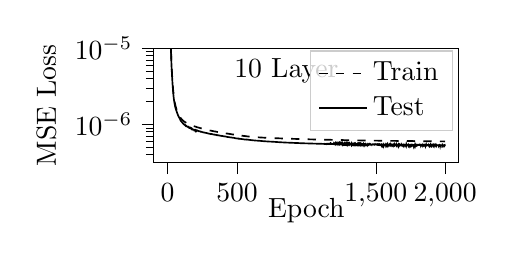
\begin{tikzpicture}

\begin{axis}[
legend cell align={left},
legend style={fill opacity=0.8, draw opacity=1, text opacity=1, draw=white!80!black},
log basis y={10},
tick align=outside,
tick pos=left,
title={10 Layer $\rare$},
title style={at={(0.45,0.85)},anchor=north},
x grid style={white!69.0196078431373!black},
xlabel={Epoch},
x label style={yshift=10pt},
xmin=-99.95, xmax=2098.95,
xtick style={color=black},
xtick = {0,500,1500,2000},
y grid style={white!69.0196078431373!black},
ylabel={MSE Loss},
ymin=3.17093839325154e-07, ymax=1e-5,
ymode=log,
ytick style={color=black},
width=0.45\textwidth,
height=0.25\textwidth
]
\addplot [semithick, black, dashed]
table {%
0 0.00997787586692721
1 0.0027661414751783
2 0.00218623768771067
3 0.00185343958390877
4 0.00115804947796278
5 0.00036777743147104
6 0.00018824286320887
7 0.000164930714039656
8 0.000153345151928079
9 0.000141543177305721
10 0.000127938025187177
11 0.000112482768548944
12 9.57521400996484e-05
13 7.92569487603032e-05
14 6.42920351929206e-05
15 5.20401717658388e-05
16 4.29740166491683e-05
17 3.62663831710961e-05
18 3.07352183917828e-05
19 2.49385155948403e-05
20 2.06156149879462e-05
21 1.71943852956247e-05
22 1.4385688823495e-05
23 1.20649838572717e-05
24 1.02233446727951e-05
25 8.78601411159252e-06
26 7.68138640933103e-06
27 6.83470541434872e-06
28 6.17248770799961e-06
29 5.6463688954409e-06
30 5.22004835283951e-06
31 4.84264568081016e-06
32 4.50758502950066e-06
33 4.20824098557659e-06
34 3.93843728591037e-06
35 3.69604697584691e-06
36 3.4781861807005e-06
37 3.27953066255304e-06
38 3.102444766796e-06
39 2.94624955324707e-06
40 2.80618139169064e-06
41 2.6809971720354e-06
42 2.57034235244191e-06
43 2.47136843603357e-06
44 2.38247599895658e-06
45 2.3052505364376e-06
46 2.2339168820622e-06
47 2.16824932778081e-06
48 2.10921677893339e-06
49 2.05554289499332e-06
50 2.00520992609654e-06
51 1.96032569562021e-06
52 1.91601798240981e-06
53 1.87716817765704e-06
54 1.84075475442569e-06
55 1.8041044749566e-06
56 1.77211888149031e-06
57 1.74144628215345e-06
58 1.71423015325445e-06
59 1.68766705314738e-06
60 1.66201588962167e-06
61 1.63708562206466e-06
62 1.61347263502876e-06
63 1.5917540299597e-06
64 1.57049718154667e-06
65 1.55085114516851e-06
66 1.53163219016506e-06
67 1.51338286417513e-06
68 1.49671406592233e-06
69 1.47951891813136e-06
70 1.4645103722728e-06
71 1.44944799347968e-06
72 1.43420475933453e-06
73 1.41955645852931e-06
74 1.40517172491172e-06
75 1.39141421908562e-06
76 1.37808219858471e-06
77 1.3657449522384e-06
78 1.3527578432786e-06
79 1.34140151624251e-06
80 1.32919058387415e-06
81 1.31819503866382e-06
82 1.30771289047971e-06
83 1.29784039592096e-06
84 1.28814695580104e-06
85 1.27880892563326e-06
86 1.27049044516525e-06
87 1.26170827212491e-06
88 1.25354349086138e-06
89 1.24524294693629e-06
90 1.23696791416705e-06
91 1.22909348488065e-06
92 1.22303059853834e-06
93 1.21662571478964e-06
94 1.20954619882241e-06
95 1.20269462843225e-06
96 1.19554730241589e-06
97 1.18936523608681e-06
98 1.18438249876363e-06
99 1.17871571490014e-06
100 1.17326355984915e-06
101 1.16720301622308e-06
102 1.16031671996097e-06
103 1.15646743591924e-06
104 1.15072228288682e-06
105 1.1456532542411e-06
106 1.14082713997732e-06
107 1.13676369537075e-06
108 1.13183904920788e-06
109 1.12775252654274e-06
110 1.12097592221971e-06
111 1.11884615537861e-06
112 1.11495200479794e-06
113 1.11073350669244e-06
114 1.10769001994981e-06
115 1.10351587494506e-06
116 1.10006028367593e-06
117 1.09647195202456e-06
118 1.09295321027503e-06
119 1.08959795028341e-06
120 1.08633151981508e-06
121 1.08298288154174e-06
122 1.0800084913285e-06
123 1.07806380844977e-06
124 1.074994691038e-06
125 1.07166258550251e-06
126 1.06880648237961e-06
127 1.06578414178671e-06
128 1.06304140217617e-06
129 1.06044994532795e-06
130 1.05643772593567e-06
131 1.0558744672835e-06
132 1.05326026272223e-06
133 1.04935598690759e-06
134 1.04676802968129e-06
135 1.04461839976011e-06
136 1.04219356757085e-06
137 1.03843377786461e-06
138 1.03679534922208e-06
139 1.03479115048799e-06
140 1.03239273369127e-06
141 1.02880143617767e-06
142 1.02687638050725e-06
143 1.02502206539157e-06
144 1.02148192920026e-06
145 1.02024824695945e-06
146 1.01793011802442e-06
147 1.01475467491241e-06
148 1.01393682172102e-06
149 1.01059575447948e-06
150 1.00912902482264e-06
151 1.0062060501923e-06
152 1.00506513257415e-06
153 1.00228589985818e-06
154 1.00133910484601e-06
155 9.99022535552285e-07
156 9.96578049466734e-07
157 9.95774760042423e-07
158 9.92670811598373e-07
159 9.90552980908888e-07
160 9.90131076179068e-07
161 9.8754623903119e-07
162 9.8556907477132e-07
163 9.85354359244184e-07
164 9.82352091568828e-07
165 9.80439722610527e-07
166 9.78883942138964e-07
167 9.78459102157103e-07
168 9.75541983876837e-07
169 9.74201690695509e-07
170 9.73315617585513e-07
171 9.7158668955899e-07
172 9.71484288783131e-07
173 9.67737080088682e-07
174 9.66393180931391e-07
175 9.64838651981381e-07
176 9.64215281697989e-07
177 9.62576921267555e-07
178 9.63217306946262e-07
179 9.60148133856364e-07
180 9.59013245392271e-07
181 9.56711457007486e-07
182 9.55200339518569e-07
183 9.53850673880652e-07
184 9.52729099026328e-07
185 9.51356085352018e-07
186 9.49982874573152e-07
187 9.48758935265914e-07
188 9.4734960742926e-07
189 9.46268320717536e-07
190 9.45888197207978e-07
191 9.43202051558956e-07
192 9.42285718593894e-07
193 9.4148136670924e-07
194 9.39797778954699e-07
195 9.38851433886612e-07
196 9.36940359082428e-07
197 9.35960853297502e-07
198 9.35100780367293e-07
199 9.33036782470253e-07
200 9.32759092336255e-07
201 9.309670438995e-07
202 9.30231287497918e-07
203 9.28388456145512e-07
204 9.28534422172334e-07
205 9.26417262860468e-07
206 9.25963449361689e-07
207 9.23892555078964e-07
208 9.23097257839345e-07
209 9.21156167748904e-07
210 9.20179683930655e-07
211 9.18629479031097e-07
212 9.17580147955732e-07
213 9.16587913565081e-07
214 9.15249802602602e-07
215 9.14260038939574e-07
216 9.13397146405259e-07
217 9.12211345678315e-07
218 9.10792389674953e-07
219 9.10044973522872e-07
220 9.09023786704211e-07
221 9.08015798756878e-07
222 9.07080938276295e-07
223 9.05977511166611e-07
224 9.05009585721928e-07
225 9.03722100105142e-07
226 9.0283103281763e-07
227 9.01766764314971e-07
228 9.00620563015764e-07
229 8.99610003187945e-07
230 8.98586724986217e-07
231 8.97490580570093e-07
232 8.96478950949131e-07
233 8.95298846074866e-07
234 8.94353904413947e-07
235 8.93204120927749e-07
236 8.923171830304e-07
237 8.90687736870177e-07
238 8.89868796548399e-07
239 8.88946101269994e-07
240 8.87893214382984e-07
241 8.86297618535537e-07
242 8.85070359657902e-07
243 8.84417957706773e-07
244 8.83675672440631e-07
245 8.8251698130648e-07
246 8.81460606791507e-07
247 8.8027023426207e-07
248 8.79355826469919e-07
249 8.78572113578002e-07
250 8.77525471793206e-07
251 8.76351880549464e-07
252 8.75500791465811e-07
253 8.74678740700574e-07
254 8.73476796158457e-07
255 8.72610606649005e-07
256 8.71706194686794e-07
257 8.70708743093473e-07
258 8.70191305182289e-07
259 8.69344236235747e-07
260 8.67789354629167e-07
261 8.66628777828282e-07
262 8.65958915056808e-07
263 8.64537149453781e-07
264 8.63818404411631e-07
265 8.62849739490912e-07
266 8.61764416811184e-07
267 8.60982841373925e-07
268 8.60051689585362e-07
269 8.59030311005427e-07
270 8.58128868173935e-07
271 8.57145231947243e-07
272 8.56545518360008e-07
273 8.55089079635718e-07
274 8.54582956577588e-07
275 8.53439548222923e-07
276 8.52625509651261e-07
277 8.52064497024685e-07
278 8.50905582069572e-07
279 8.50112307404061e-07
280 8.49598813260855e-07
281 8.4875707469223e-07
282 8.4775906213963e-07
283 8.4675666619205e-07
284 8.46309231747e-07
285 8.45124665829644e-07
286 8.44529056251986e-07
287 8.43495970570984e-07
288 8.42961660282526e-07
289 8.41671420289458e-07
290 8.41705411914972e-07
291 8.40604265988532e-07
292 8.39964006132732e-07
293 8.38750670340005e-07
294 8.3819956410025e-07
295 8.37723511324384e-07
296 8.36425500693849e-07
297 8.35761372655952e-07
298 8.35393352815572e-07
299 8.3392940771887e-07
300 8.3388055014666e-07
301 8.32478889208232e-07
302 8.32139470674065e-07
303 8.31678217167564e-07
304 8.30812586201546e-07
305 8.30091150533008e-07
306 8.29310000142414e-07
307 8.28749091709824e-07
308 8.2756600025391e-07
309 8.27514076803482e-07
310 8.26390768622787e-07
311 8.25961606182091e-07
312 8.25162235912558e-07
313 8.24495962177707e-07
314 8.24095709617723e-07
315 8.22966658319046e-07
316 8.21936873251161e-07
317 8.21767470569057e-07
318 8.20922504203736e-07
319 8.20247862861834e-07
320 8.19370113532614e-07
321 8.18635833951475e-07
322 8.17986851899377e-07
323 8.17315450689193e-07
324 8.1666383891843e-07
325 8.16427804124942e-07
326 8.15375180422961e-07
327 8.15192657825037e-07
328 8.14120937434382e-07
329 8.13174602825484e-07
330 8.1293584187847e-07
331 8.11936721930806e-07
332 8.11085818554602e-07
333 8.10528149429501e-07
334 8.09983656409941e-07
335 8.08851426143065e-07
336 8.08121500682546e-07
337 8.08130491662951e-07
338 8.07360241225297e-07
339 8.06781943225587e-07
340 8.06020081228098e-07
341 8.05330066299348e-07
342 8.04786609791108e-07
343 8.0464047090345e-07
344 8.03382348692594e-07
345 8.03091622429974e-07
346 8.03480803682533e-07
347 8.01579474654091e-07
348 8.0091967774365e-07
349 8.01363648946563e-07
350 7.99436845767332e-07
351 7.99345849031852e-07
352 7.98882536855672e-07
353 7.97898566048616e-07
354 7.98836069549225e-07
355 7.98981313806735e-07
356 7.97069268514861e-07
357 7.96280659386639e-07
358 7.96522883803164e-07
359 7.94783968302681e-07
360 7.94133767442418e-07
361 7.94591968116265e-07
362 7.92818375458637e-07
363 7.92365432204178e-07
364 7.91729609915137e-07
365 7.92124033381469e-07
366 7.9021502497767e-07
367 7.89800760259141e-07
368 7.89006110096579e-07
369 7.89422273101081e-07
370 7.87633119500697e-07
371 7.87470235025012e-07
372 7.86781127885661e-07
373 7.87345359412939e-07
374 7.85442462444053e-07
375 7.85028574483704e-07
376 7.84489331238092e-07
377 7.83982934024152e-07
378 7.84435161477859e-07
379 7.82677077467042e-07
380 7.8204591821418e-07
381 7.81801198940002e-07
382 7.81111819321723e-07
383 7.81425274823278e-07
384 7.7998786557032e-07
385 7.79324741330356e-07
386 7.78943699941692e-07
387 7.78382946805323e-07
388 7.7774481707138e-07
389 7.78080912994028e-07
390 7.76618715718769e-07
391 7.76134723423638e-07
392 7.75627843495386e-07
393 7.74918021193116e-07
394 7.74431415038634e-07
395 7.74660446609232e-07
396 7.73305947575409e-07
397 7.72896880562257e-07
398 7.72197305280997e-07
399 7.71702392796669e-07
400 7.71071945763424e-07
401 7.70523813088175e-07
402 7.70097182538621e-07
403 7.7021479600603e-07
404 7.68894578584423e-07
405 7.68398064082021e-07
406 7.67811163484566e-07
407 7.67315257036216e-07
408 7.66777737169377e-07
409 7.66156092197434e-07
410 7.65690696312049e-07
411 7.65130233787659e-07
412 7.6555170792858e-07
413 7.64065328610286e-07
414 7.63505121966546e-07
415 7.63133862619725e-07
416 7.62454071889351e-07
417 7.62014022313906e-07
418 7.6143167035525e-07
419 7.60892476279196e-07
420 7.60415168230111e-07
421 7.59914973372133e-07
422 7.5941622890241e-07
423 7.60389407474804e-07
424 7.58777384561427e-07
425 7.58338006789927e-07
426 7.57724335500143e-07
427 7.57657803433176e-07
428 7.56923721269232e-07
429 7.56353567965107e-07
430 7.56923098862217e-07
431 7.55219046823186e-07
432 7.54618819826192e-07
433 7.54311231389693e-07
434 7.53780425611694e-07
435 7.54422887609962e-07
436 7.52576872230293e-07
437 7.52243586475743e-07
438 7.51672492100397e-07
439 7.52297821776438e-07
440 7.50493718726375e-07
441 7.50091651326557e-07
442 7.49571382499425e-07
443 7.5027601661759e-07
444 7.48633131451015e-07
445 7.48203038369866e-07
446 7.47641490107753e-07
447 7.4706847775019e-07
448 7.47778209245098e-07
449 7.45882051290891e-07
450 7.45447632596097e-07
451 7.45004974220365e-07
452 7.45590436821431e-07
453 7.44075579518722e-07
454 7.43488029229411e-07
455 7.4302814456928e-07
456 7.43562355694394e-07
457 7.42126745706173e-07
458 7.41440271383453e-07
459 7.41023272865959e-07
460 7.42221455794834e-07
461 7.39916425203546e-07
462 7.39315465096979e-07
463 7.38942567977574e-07
464 7.39466763462815e-07
465 7.38114260798284e-07
466 7.37723011752678e-07
467 7.38328398483645e-07
468 7.36677821834064e-07
469 7.36189456091552e-07
470 7.36971248016971e-07
471 7.35291715386666e-07
472 7.34859717340441e-07
473 7.35544233293695e-07
474 7.33993297529878e-07
475 7.33437984763441e-07
476 7.34147434599208e-07
477 7.32526463366412e-07
478 7.32113129146228e-07
479 7.32783056690778e-07
480 7.31102353171309e-07
481 7.30759978779361e-07
482 7.30174026074337e-07
483 7.3101718700741e-07
484 7.29139022212166e-07
485 7.28747309921118e-07
486 7.29511678514427e-07
487 7.27845423909912e-07
488 7.27509910404933e-07
489 7.27898909303804e-07
490 7.25985288198672e-07
491 7.26988534040629e-07
492 7.26433349939271e-07
493 7.24913795409066e-07
494 7.25639360695141e-07
495 7.25110006783325e-07
496 7.23576190097219e-07
497 7.24332362437963e-07
498 7.23792091548603e-07
499 7.22295086035274e-07
500 7.23148807196594e-07
501 7.22562276394001e-07
502 7.21028598093199e-07
503 7.21920047169533e-07
504 7.20162841702177e-07
505 7.21097849861962e-07
506 7.20601577768321e-07
507 7.18964301626102e-07
508 7.19790344447802e-07
509 7.19423874585345e-07
510 7.17816719657094e-07
511 7.18529795136646e-07
512 7.17035474110617e-07
513 7.17842366498189e-07
514 7.173693042688e-07
515 7.15891436129823e-07
516 7.16593398948362e-07
517 7.16193349916239e-07
518 7.15836237418444e-07
519 7.13896747583931e-07
520 7.14747440071051e-07
521 7.14939811359727e-07
522 7.14682133747146e-07
523 7.14109896080117e-07
524 7.12665502788923e-07
525 7.13412247876022e-07
526 7.12840395792114e-07
527 7.1258078847336e-07
528 7.1094341305411e-07
529 7.11800691419739e-07
530 7.11041270108126e-07
531 7.11053048263466e-07
532 7.09551945874409e-07
533 7.10300355095228e-07
534 7.10044622053374e-07
535 7.08126653066188e-07
536 7.09192354179322e-07
537 7.08688509973854e-07
538 7.08473750933081e-07
539 7.0703383852333e-07
540 7.07924062425036e-07
541 7.07072048214741e-07
542 7.05930014561318e-07
543 7.06833243867777e-07
544 7.06151251620213e-07
545 7.05789116310029e-07
546 7.05411095324848e-07
547 7.03952515351602e-07
548 7.04824918869917e-07
549 7.04396891237025e-07
550 7.04121892809439e-07
551 7.03592790472385e-07
552 7.02295799982267e-07
553 7.03159633289374e-07
554 7.02392406822128e-07
555 7.02389151811644e-07
556 7.02069595888588e-07
557 7.00544815430249e-07
558 7.01544812031329e-07
559 7.01071055104308e-07
560 7.00843794945172e-07
561 7.00298507183561e-07
562 6.99028340818586e-07
563 6.9988211890859e-07
564 6.99153588470836e-07
565 6.99094921657206e-07
566 6.98874052901033e-07
567 6.97493815380312e-07
568 6.9732204678985e-07
569 6.96886004035946e-07
570 6.96496134878544e-07
571 6.96340423658626e-07
572 6.9577226418005e-07
573 6.95301015184668e-07
574 6.94970092226299e-07
575 6.94665715130327e-07
576 6.94327597415167e-07
577 6.9397252194392e-07
578 6.93629053131417e-07
579 6.93304834925357e-07
580 6.92961221275823e-07
581 6.92612403483395e-07
582 6.92295116081709e-07
583 6.92008054087978e-07
584 6.91836038868132e-07
585 6.91154041760456e-07
586 6.91039159349316e-07
587 6.90780433998839e-07
588 6.90375913677599e-07
589 6.90120593674237e-07
590 6.89844487624214e-07
591 6.89540247705622e-07
592 6.8927526524476e-07
593 6.88991556458518e-07
594 6.88708317511555e-07
595 6.88413684557077e-07
596 6.88122735454044e-07
597 6.87847310999246e-07
598 6.87655565940304e-07
599 6.873611031466e-07
600 6.8711852216552e-07
601 6.86813203969905e-07
602 6.86521028598008e-07
603 6.86258257005079e-07
604 6.86011237931439e-07
605 6.85736956057781e-07
606 6.8547543475006e-07
607 6.85227141644873e-07
608 6.84974181766052e-07
609 6.84731802891747e-07
610 6.84444454293498e-07
611 6.84201174820487e-07
612 6.83949088440272e-07
613 6.83735282066777e-07
614 6.83597051065021e-07
615 6.83230357168441e-07
616 6.82977046281508e-07
617 6.82744479377107e-07
618 6.82628084632597e-07
619 6.82269299900895e-07
620 6.82057781943968e-07
621 6.81825706507766e-07
622 6.81707034459578e-07
623 6.81389691763457e-07
624 6.81201359242323e-07
625 6.81054129145764e-07
626 6.8075853309324e-07
627 6.80542225936165e-07
628 6.80400173507678e-07
629 6.80067346735314e-07
630 6.79983958491448e-07
631 6.79618614057631e-07
632 6.79393168169895e-07
633 6.79165578233665e-07
634 6.79077912963066e-07
635 6.78772824926455e-07
636 6.78559704212489e-07
637 6.78351354096662e-07
638 6.78243983884386e-07
639 6.77901727698327e-07
640 6.77708650769659e-07
641 6.77525354845443e-07
642 6.77312835492216e-07
643 6.77094021853009e-07
644 6.7693512350786e-07
645 6.76660766927739e-07
646 6.76465998878939e-07
647 6.7620693066317e-07
648 6.76058081367614e-07
649 6.75807865121669e-07
650 6.75675274962373e-07
651 6.75309103939981e-07
652 6.75240928430298e-07
653 6.75009894337109e-07
654 6.74884714669588e-07
655 6.7469262417319e-07
656 6.74492794075832e-07
657 6.74472121843905e-07
658 6.74072660487468e-07
659 6.74126479594861e-07
660 6.73871772562507e-07
661 6.73676320815275e-07
662 6.73381162670239e-07
663 6.73315533632035e-07
664 6.7304010840985e-07
665 6.7279634778572e-07
666 6.72624413653011e-07
667 6.72622655784494e-07
668 6.72328725286775e-07
669 6.72171628352203e-07
670 6.72120275240218e-07
671 6.72108327890442e-07
672 6.71769079815476e-07
673 6.71592175606861e-07
674 6.7153022288835e-07
675 6.71228376674549e-07
676 6.71063214738865e-07
677 6.70862587298871e-07
678 6.70727474243904e-07
679 6.70538763273498e-07
680 6.70397458648608e-07
681 6.70331136205959e-07
682 6.70071903499547e-07
683 6.69920863757056e-07
684 6.69779470129583e-07
685 6.69620603034105e-07
686 6.69458129848977e-07
687 6.6930754940131e-07
688 6.69167233667167e-07
689 6.68956220224004e-07
690 6.68770538680974e-07
691 6.68667876396967e-07
692 6.68520957177066e-07
693 6.68362044635273e-07
694 6.68231087544768e-07
695 6.68063874257996e-07
696 6.67905007389891e-07
697 6.67740694836993e-07
698 6.67615698802138e-07
699 6.67491615800486e-07
700 6.67331059744924e-07
701 6.67199185485856e-07
702 6.67054764520003e-07
703 6.66892555187815e-07
704 6.66757220614045e-07
705 6.6661704566684e-07
706 6.66472319977629e-07
707 6.66348736558575e-07
708 6.66208892795339e-07
709 6.66104842267146e-07
710 6.65947033539283e-07
711 6.6583568202816e-07
712 6.65676333156284e-07
713 6.65566532433104e-07
714 6.65371252381419e-07
715 6.65273846124137e-07
716 6.65145204777673e-07
717 6.6501357501636e-07
718 6.64885187660502e-07
719 6.64747493914319e-07
720 6.64656038921407e-07
721 6.64518116366253e-07
722 6.64384310013588e-07
723 6.6426489875937e-07
724 6.64103254891302e-07
725 6.6400623869356e-07
726 6.6387511243704e-07
727 6.63760887292142e-07
728 6.63594443778948e-07
729 6.6352547675308e-07
730 6.63392976136379e-07
731 6.63245974934057e-07
732 6.63125168372858e-07
733 6.63018874917043e-07
734 6.62882144197852e-07
735 6.62734271159593e-07
736 6.62517572180832e-07
737 6.6241604606887e-07
738 6.62473698085364e-07
739 6.62516929139656e-07
740 6.62498065295836e-07
741 6.61815979839275e-07
742 6.61530765412976e-07
743 6.61442542394752e-07
744 6.61331088323891e-07
745 6.61209408832519e-07
746 6.6109859224639e-07
747 6.6099788502072e-07
748 6.60889263187414e-07
749 6.60740850307207e-07
750 6.60631029802516e-07
751 6.60538422906143e-07
752 6.60393012481109e-07
753 6.60271693462278e-07
754 6.60180221544238e-07
755 6.60043354130835e-07
756 6.59950334664927e-07
757 6.59887545353399e-07
758 6.5971084376315e-07
759 6.59582626255428e-07
760 6.59522363278597e-07
761 6.59398176679815e-07
762 6.59279328061757e-07
763 6.59160926986146e-07
764 6.59018419938207e-07
765 6.58968605165455e-07
766 6.58780548107529e-07
767 6.58640463925053e-07
768 6.58545901032426e-07
769 6.58429381942938e-07
770 6.58341001013696e-07
771 6.58279398663808e-07
772 6.58103613247363e-07
773 6.58032226553473e-07
774 6.5792477641935e-07
775 6.57836251804156e-07
776 6.57792503417909e-07
777 6.57651318391572e-07
778 6.57547617464616e-07
779 6.57399611057485e-07
780 6.57286304786453e-07
781 6.57153251651721e-07
782 6.5710807548669e-07
783 6.56900221926549e-07
784 6.56799596583824e-07
785 6.56696743305929e-07
786 6.56575473740872e-07
787 6.56487851685483e-07
788 6.56370081244972e-07
789 6.56292135957415e-07
790 6.56130607339378e-07
791 6.56064941154e-07
792 6.56011381011012e-07
793 6.55829648934514e-07
794 6.55786200027819e-07
795 6.55607685331461e-07
796 6.55609785056299e-07
797 6.55533220481175e-07
798 6.55394131726439e-07
799 6.55311715917151e-07
800 6.55156520764422e-07
801 6.55102531055718e-07
802 6.55082887604408e-07
803 6.54888119228758e-07
804 6.54802214071992e-07
805 6.5473559047291e-07
806 6.54574609910696e-07
807 6.54500922465218e-07
808 6.54382220616867e-07
809 6.54305573817737e-07
810 6.5420019161877e-07
811 6.54057651630069e-07
812 6.53967765671837e-07
813 6.53819775891407e-07
814 6.53770412583299e-07
815 6.53644654022401e-07
816 6.53591989035362e-07
817 6.53487234302474e-07
818 6.53435297138572e-07
819 6.53194102852694e-07
820 6.53198145187162e-07
821 6.5311538847368e-07
822 6.52892069282984e-07
823 6.52899213022806e-07
824 6.52815578064292e-07
825 6.52532915339066e-07
826 6.5250298719377e-07
827 6.52467241110344e-07
828 6.52352714354265e-07
829 6.52214292244935e-07
830 6.52175464963989e-07
831 6.52048443271269e-07
832 6.51983712870674e-07
833 6.51903975750656e-07
834 6.51790568511501e-07
835 6.51704363789918e-07
836 6.51591102098337e-07
837 6.51535222814914e-07
838 6.5140828783683e-07
839 6.51308421680596e-07
840 6.51213768250614e-07
841 6.51116864844425e-07
842 6.50987768693767e-07
843 6.50862097572258e-07
844 6.50764789384084e-07
845 6.50686730963912e-07
846 6.50605446963937e-07
847 6.50517625658154e-07
848 6.49935367121657e-07
849 6.49951558187922e-07
850 6.49781994908949e-07
851 6.49812969228947e-07
852 6.4962381597411e-07
853 6.49715427286424e-07
854 6.49609696424136e-07
855 6.49503299598564e-07
856 6.49437240753059e-07
857 6.4924598638072e-07
858 6.49154591329193e-07
859 6.49055806263732e-07
860 6.48968337969791e-07
861 6.48860881113933e-07
862 6.48779707205449e-07
863 6.4869935371803e-07
864 6.48607655406863e-07
865 6.48494430663504e-07
866 6.48387495814973e-07
867 6.48355465315831e-07
868 6.4823302085415e-07
869 6.48177903727287e-07
870 6.48068991381479e-07
871 6.48002301730344e-07
872 6.47880534643264e-07
873 6.4779980566243e-07
874 6.47472709502495e-07
875 6.47573727789563e-07
876 6.47521113151583e-07
877 6.47460983415726e-07
878 6.47327359146743e-07
879 6.47256306294253e-07
880 6.47165816758388e-07
881 6.47062579616886e-07
882 6.46873130364156e-07
883 6.46932409637202e-07
884 6.4678064497059e-07
885 6.46794917827265e-07
886 6.4658947853502e-07
887 6.46604447453569e-07
888 6.46413081099695e-07
889 6.46435930761413e-07
890 6.46238205860072e-07
891 6.46160109269545e-07
892 6.46079087459839e-07
893 6.45998969318384e-07
894 6.45898591372429e-07
895 6.45816730695969e-07
896 6.45777476066201e-07
897 6.45704528096758e-07
898 6.45561784040183e-07
899 6.45402865401934e-07
900 6.45395685438643e-07
901 6.45250818593013e-07
902 6.45247586589903e-07
903 6.45016569762902e-07
904 6.45096973528325e-07
905 6.44992183836734e-07
906 6.44879979844859e-07
907 6.44814044164832e-07
908 6.44536055304457e-07
909 6.44651230615523e-07
910 6.44630252224943e-07
911 6.44534238688266e-07
912 6.44403965878837e-07
913 6.44269876133308e-07
914 6.44109464232656e-07
915 6.44056983475139e-07
916 6.44181476729955e-07
917 6.44011751091966e-07
918 6.43851985074662e-07
919 6.43799305493076e-07
920 6.43708418380129e-07
921 6.43616032121486e-07
922 6.43390352038864e-07
923 6.43459086845155e-07
924 6.43066392427727e-07
925 6.43326589468529e-07
926 6.43231603277172e-07
927 6.42995318642647e-07
928 6.43065223883355e-07
929 6.42968633215446e-07
930 6.42634859744362e-07
931 6.42847502362542e-07
932 6.42573602135599e-07
933 6.42576249461513e-07
934 6.42420869482407e-07
935 6.42509780959699e-07
936 6.42260338906908e-07
937 6.42345372426689e-07
938 6.4186560094015e-07
939 6.42131707621729e-07
940 6.41876858665569e-07
941 6.41937691256089e-07
942 6.41715006921117e-07
943 6.41790332380765e-07
944 6.41556473468086e-07
945 6.415050187627e-07
946 6.41448093148256e-07
947 6.41452986968716e-07
948 6.41207829275459e-07
949 6.41160052467171e-07
950 6.41136324560421e-07
951 6.41156462506842e-07
952 6.4103641173574e-07
953 6.40879574191899e-07
954 6.40985946901651e-07
955 6.40758436617261e-07
956 6.40720444295084e-07
957 6.40529553727731e-07
958 6.40474377917144e-07
959 6.40498605775974e-07
960 6.40255618591823e-07
961 6.40319487331453e-07
962 6.40329926909544e-07
963 6.40118906979126e-07
964 6.40069182985315e-07
965 6.39933080719857e-07
966 6.40022533211493e-07
967 6.39830953474529e-07
968 6.39713040214929e-07
969 6.39593101901426e-07
970 6.39774005406935e-07
971 6.39434521559679e-07
972 6.39282294187637e-07
973 6.39523240408835e-07
974 6.39073064718332e-07
975 6.39149466316269e-07
976 6.39264868198097e-07
977 6.38937482264623e-07
978 6.3891833339369e-07
979 6.3900999825961e-07
980 6.38726525863831e-07
981 6.38650845402822e-07
982 6.38661012288821e-07
983 6.38419105449373e-07
984 6.38549863495541e-07
985 6.38299137555975e-07
986 6.38424846982843e-07
987 6.38142738338843e-07
988 6.38220265770428e-07
989 6.38023431044132e-07
990 6.38141142715654e-07
991 6.37875260373733e-07
992 6.37939418027145e-07
993 6.37722096641369e-07
994 6.3776769428614e-07
995 6.37635073331921e-07
996 6.37635214005172e-07
997 6.37495254942166e-07
998 6.3745381473268e-07
999 6.37371561651889e-07
1000 6.36697234590144e-07
1001 6.36720888294917e-07
1002 6.36737104024121e-07
1003 6.36686584201129e-07
1004 6.36586772294834e-07
1005 6.36517155868432e-07
1006 6.36517348780785e-07
1007 6.36441783626651e-07
1008 6.3637201033373e-07
1009 6.36290345994439e-07
1010 6.36226407571883e-07
1011 6.36187908853003e-07
1012 6.36128972693939e-07
1013 6.36090735575578e-07
1014 6.3589234423489e-07
1015 6.35912154805851e-07
1016 6.35904042837865e-07
1017 6.35763122460276e-07
1018 6.35666576634719e-07
1019 6.3564752967693e-07
1020 6.35538853181572e-07
1021 6.35491918373532e-07
1022 6.35451334389359e-07
1023 6.35415595198197e-07
1024 6.35248154431167e-07
1025 6.35240329302178e-07
1026 6.35150410481344e-07
1027 6.35137976871647e-07
1028 6.34976308155899e-07
1029 6.35017855039166e-07
1030 6.3482607657761e-07
1031 6.34881822449529e-07
1032 6.34690630576529e-07
1033 6.34540902638037e-07
1034 6.34473359724552e-07
1035 6.34451190421714e-07
1036 6.34297449984445e-07
1037 6.34270674453319e-07
1038 6.34141945823785e-07
1039 6.34231479885727e-07
1040 6.34136626601389e-07
1041 6.34082943328451e-07
1042 6.3395456306381e-07
1043 6.33960346824836e-07
1044 6.33853544790952e-07
1045 6.33788128311608e-07
1046 6.33753139354098e-07
1047 6.33628680830611e-07
1048 6.33625172490326e-07
1049 6.33516750120577e-07
1050 6.33459435064765e-07
1051 6.33394688364319e-07
1052 6.33326460899752e-07
1053 6.33260135010971e-07
1054 6.33217650971574e-07
1055 6.33124233907267e-07
1056 6.33073544925367e-07
1057 6.32994399367703e-07
1058 6.32937160020219e-07
1059 6.32863034105924e-07
1060 6.32802857673198e-07
1061 6.327211272108e-07
1062 6.32664070593592e-07
1063 6.32609571134424e-07
1064 6.3261294997119e-07
1065 6.32557479264051e-07
1066 6.32472583347976e-07
1067 6.32388676500284e-07
1068 6.3235371713688e-07
1069 6.32262299873787e-07
1070 6.32186852847383e-07
1071 6.32157002080191e-07
1072 6.32051000330591e-07
1073 6.31951863908853e-07
1074 6.31979543818772e-07
1075 6.31833903980805e-07
1076 6.31841321954596e-07
1077 6.31720386728318e-07
1078 6.31670170619714e-07
1079 6.31639167558262e-07
1080 6.31551888616855e-07
1081 6.31490619177555e-07
1082 6.31423811270793e-07
1083 6.3135732366959e-07
1084 6.31311455016714e-07
1085 6.31243087482858e-07
1086 6.31197074852707e-07
1087 6.31128118996571e-07
1088 6.31093993149534e-07
1089 6.31002973804584e-07
1090 6.30930024748011e-07
1091 6.30873843036284e-07
1092 6.30818468749794e-07
1093 6.30774500507414e-07
1094 6.30719061497587e-07
1095 6.30654274829112e-07
1096 6.30573381890542e-07
1097 6.30514150955719e-07
1098 6.30455811105435e-07
1099 6.30417263671745e-07
1100 6.303295307859e-07
1101 6.30289127698802e-07
1102 6.30195487040908e-07
1103 6.30157178008517e-07
1104 6.30050639735202e-07
1105 6.29987743629101e-07
1106 6.29968577783302e-07
1107 6.29872791670039e-07
1108 6.29852591870872e-07
1109 6.29763205395761e-07
1110 6.2972433978814e-07
1111 6.29685811993852e-07
1112 6.29570583363659e-07
1113 6.29555979784868e-07
1114 6.29505421251508e-07
1115 6.29378778313594e-07
1116 6.29395147583978e-07
1117 6.29327122219081e-07
1118 6.29239093782985e-07
1119 6.29181523294164e-07
1120 6.29151311549947e-07
1121 6.29059220806027e-07
1122 6.29024048642179e-07
1123 6.28953817965794e-07
1124 6.28911244270114e-07
1125 6.28805891778938e-07
1126 6.28756066198832e-07
1127 6.28648164230583e-07
1128 6.28306397643996e-07
1129 6.28687460732635e-07
1130 6.2848032885654e-07
1131 6.28135447911404e-07
1132 6.28400187004274e-07
1133 6.28573363961493e-07
1134 6.28527363033982e-07
1135 6.28527280390756e-07
1136 6.28343305770329e-07
1137 6.28284698507287e-07
1138 6.2812800601364e-07
1139 6.28083045576488e-07
1140 6.28054853891058e-07
1141 6.28019043531936e-07
1142 6.27906697488356e-07
1143 6.27742714229385e-07
1144 6.27365253272671e-07
1145 6.27446661880526e-07
1146 6.27488955871058e-07
1147 6.27701524173574e-07
1148 6.27380187211202e-07
1149 6.27639201667307e-07
1150 6.2732651976205e-07
1151 6.27196206636427e-07
1152 6.27453849801896e-07
1153 6.27290091358645e-07
1154 6.27293938102014e-07
1155 6.27100247442058e-07
1156 6.26845826687372e-07
1157 6.27136329399036e-07
1158 6.26958845828085e-07
1159 6.27028462695023e-07
1160 6.26799966369163e-07
1161 6.26518928804387e-07
1162 6.26466177664042e-07
1163 6.26487830309941e-07
1164 6.26460136622597e-07
1165 6.26553522593554e-07
1166 6.2658400442217e-07
1167 6.26421702463631e-07
1168 6.26354288016273e-07
1169 6.26202877917592e-07
1170 6.26266790412444e-07
1171 6.26346333575611e-07
1172 6.26213740538617e-07
1173 6.2591202649287e-07
1174 6.26159682411753e-07
1175 6.259679466325e-07
1176 6.25821323929188e-07
1177 6.25983454000334e-07
1178 6.25770567594941e-07
1179 6.25582370801681e-07
1180 6.25654848079193e-07
1181 6.25532107612514e-07
1182 6.2545592751917e-07
1183 6.25413862280766e-07
1184 6.25349340801051e-07
1185 6.25261259557419e-07
1186 6.25203425371978e-07
1187 6.25166111447584e-07
1188 6.25094666915516e-07
1189 6.25081710083464e-07
1190 6.25006898232527e-07
1191 6.24934165074365e-07
1192 6.24913404614347e-07
1193 6.24911467220102e-07
1194 6.24548951755344e-07
1195 6.24694442166174e-07
1196 6.24773008453872e-07
1197 6.24621071231957e-07
1198 6.2450013277271e-07
1199 6.24621874457887e-07
1200 6.24454692619736e-07
1201 6.24370407393826e-07
1202 6.2447302522628e-07
1203 6.24262143524845e-07
1204 6.24315219837968e-07
1205 6.2430981112982e-07
1206 6.23796075679195e-07
1207 6.24177096320011e-07
1208 6.24049105802271e-07
1209 6.24054203349544e-07
1210 6.24027001990157e-07
1211 6.23865109787403e-07
1212 6.23932852477083e-07
1213 6.23779870181807e-07
1214 6.23787094262696e-07
1215 6.23741608634987e-07
1216 6.23713004550552e-07
1217 6.23544608970405e-07
1218 6.23572001856587e-07
1219 6.23602649540089e-07
1220 6.23225978060304e-07
1221 6.23518592469452e-07
1222 6.23039261583358e-07
1223 6.23288506076847e-07
1224 6.23076261497602e-07
1225 6.23334286977695e-07
1226 6.23120273957056e-07
1227 6.23057992385156e-07
1228 6.2310072766536e-07
1229 6.22905203400137e-07
1230 6.23071342417347e-07
1231 6.22551743603594e-07
1232 6.22838785815816e-07
1233 6.22911618577859e-07
1234 6.22436094097623e-07
1235 6.2257276290012e-07
1236 6.22675055979016e-07
1237 6.22591451126198e-07
1238 6.22482214389208e-07
1239 6.22608929845114e-07
1240 6.22082830332715e-07
1241 6.22355137487318e-07
1242 6.22401920892912e-07
1243 6.22228115553014e-07
1244 6.22168779464971e-07
1245 6.2226912954344e-07
1246 6.21835941025495e-07
1247 6.22107425449769e-07
1248 6.22095544343892e-07
1249 6.21943532365776e-07
1250 6.21878639350371e-07
1251 6.21777342473706e-07
1252 6.21807686485454e-07
1253 6.21633627901019e-07
1254 6.21770785983244e-07
1255 6.21682074758212e-07
1256 6.21532353186183e-07
1257 6.21157554036245e-07
1258 6.21374166421163e-07
1259 6.21383820664789e-07
1260 6.21448532641011e-07
1261 6.21237848690726e-07
1262 6.21411155641738e-07
1263 6.20860587424943e-07
1264 6.2109406439248e-07
1265 6.21135994300914e-07
1266 6.21238524701084e-07
1267 6.20719478952481e-07
1268 6.20863639028357e-07
1269 6.21026825456283e-07
1270 6.20972499071115e-07
1271 6.20547807017147e-07
1272 6.20815331657809e-07
1273 6.20883732374011e-07
1274 6.20434088780542e-07
1275 6.20376438746462e-07
1276 6.2064274709428e-07
1277 6.20666749313159e-07
1278 6.20157986659819e-07
1279 6.20282532104e-07
1280 6.20512788032102e-07
1281 6.20443126081227e-07
1282 6.19954360075781e-07
1283 6.20158316202435e-07
1284 6.20412783675306e-07
1285 6.19787940749461e-07
1286 6.20167513709191e-07
1287 6.19920055640932e-07
1288 6.19938900399575e-07
1289 6.2001241861509e-07
1290 6.19576977349823e-07
1291 6.19768135450727e-07
1292 6.19923710424075e-07
1293 6.19364097445896e-07
1294 6.19723660356897e-07
1295 6.19799817101807e-07
1296 6.19224814414565e-07
1297 6.19575253921312e-07
1298 6.1951230144075e-07
1299 6.19440844417341e-07
1300 6.19388264468057e-07
1301 6.1928821070012e-07
1302 6.18971549577907e-07
1303 6.19309097317e-07
1304 6.18896740419927e-07
1305 6.19233279984144e-07
1306 6.18862542118848e-07
1307 6.1904855721906e-07
1308 6.19084869462938e-07
1309 6.18728734835372e-07
1310 6.19067870623269e-07
1311 6.18833963194731e-07
1312 6.18797829730511e-07
1313 6.18840376517937e-07
1314 6.18354753008532e-07
1315 6.18526108105755e-07
1316 6.18729250248862e-07
1317 6.18316310337263e-07
1318 6.18493220983396e-07
1319 6.1857565151513e-07
1320 6.18553323434412e-07
1321 6.18287408251206e-07
1322 6.18182901995112e-07
1323 6.18168552804832e-07
1324 6.18295116474599e-07
1325 6.18236038974373e-07
1326 6.18178005744596e-07
1327 6.18093473242709e-07
1328 6.17960725605826e-07
1329 6.17843770534421e-07
1330 6.18153380194997e-07
1331 6.1793422157308e-07
1332 6.17757560888776e-07
1333 6.1783743137056e-07
1334 6.17917767534948e-07
1335 6.17540525162497e-07
1336 6.17705096779275e-07
1337 6.17609444908851e-07
1338 6.17570422804192e-07
1339 6.17073546720803e-07
1340 6.17361359793733e-07
1341 6.17218927558838e-07
1342 6.1731549609334e-07
1343 6.16839265717317e-07
1344 6.17278455536052e-07
1345 6.16886698999508e-07
1346 6.17145374242512e-07
1347 6.16674280522034e-07
1348 6.16949876508954e-07
1349 6.16746271418833e-07
1350 6.17063569656295e-07
1351 6.1651876738722e-07
1352 6.16958195287509e-07
1353 6.16493237330928e-07
1354 6.16818991467483e-07
1355 6.16564756263926e-07
1356 6.16465375699704e-07
1357 6.1670159974625e-07
1358 6.16341221103767e-07
1359 6.164012397889e-07
1360 6.16298516355584e-07
1361 6.16462023430131e-07
1362 6.16257752142246e-07
1363 6.16205831555305e-07
1364 6.16200928298838e-07
1365 6.16331213180388e-07
1366 6.15774696939297e-07
1367 6.1614706064006e-07
1368 6.16303828067544e-07
1369 6.15772465287989e-07
1370 6.16175163123955e-07
1371 6.15761831603834e-07
1372 6.16118617230654e-07
1373 6.15417715017941e-07
1374 6.15825617352073e-07
1375 6.15959238160713e-07
1376 6.1554938204722e-07
1377 6.1578529990669e-07
1378 6.15404216532056e-07
1379 6.15805073294951e-07
1380 6.15045303192119e-07
1381 6.15779943856865e-07
1382 6.15239680826107e-07
1383 6.15575325518591e-07
1384 6.15164999260287e-07
1385 6.15541761249006e-07
1386 6.1481267056962e-07
1387 6.15518598799269e-07
1388 6.14974511393029e-07
1389 6.15256523204266e-07
1390 6.1495169554604e-07
1391 6.15171495873312e-07
1392 6.14589822056644e-07
1393 6.15063232331181e-07
1394 6.15107449206675e-07
1395 6.14662685840983e-07
1396 6.1502810259384e-07
1397 6.14590154093264e-07
1398 6.14612481669496e-07
1399 6.14802560768624e-07
1400 6.14702865100014e-07
1401 6.14827589217271e-07
1402 6.14387261038019e-07
1403 6.14532386492783e-07
1404 6.14365300663167e-07
1405 6.14513860909938e-07
1406 6.14463790768127e-07
1407 6.14669436131976e-07
1408 6.14088050312489e-07
1409 6.14400729553211e-07
1410 6.14347149664241e-07
1411 6.14008724106441e-07
1412 6.14388912921982e-07
1413 6.13885905003997e-07
1414 6.14030799852117e-07
1415 6.14084501023626e-07
1416 6.14049639672487e-07
1417 6.14017295546887e-07
1418 6.13979460368341e-07
1419 6.14067722430889e-07
1420 6.1396852149187e-07
1421 6.13854022716964e-07
1422 6.13682396014781e-07
1423 6.13604328492556e-07
1424 6.13541604060686e-07
1425 6.13372681478097e-07
1426 6.13554293892093e-07
1427 6.13180419733794e-07
1428 6.13455641953919e-07
1429 6.1348410481088e-07
1430 6.13415493866398e-07
1431 6.13489517483856e-07
1432 6.12983758479402e-07
1433 6.13290954696311e-07
1434 6.13153399413591e-07
1435 6.13249425313711e-07
1436 6.13075842231581e-07
1437 6.1320476547877e-07
1438 6.13227797749971e-07
1439 6.12789343271913e-07
1440 6.13057139688067e-07
1441 6.13030189320796e-07
1442 6.12636833110969e-07
1443 6.12816545171313e-07
1444 6.12819367759698e-07
1445 6.12868730669902e-07
1446 6.12897299447468e-07
1447 6.12634370639853e-07
1448 6.12377568522504e-07
1449 6.12560680650631e-07
1450 6.1260865675905e-07
1451 6.12693906937523e-07
1452 6.12507754290448e-07
1453 6.12503317547919e-07
1454 6.12373988857939e-07
1455 6.12564684573158e-07
1456 6.12393487315899e-07
1457 6.12160607012413e-07
1458 6.12446222532981e-07
1459 6.12120268648653e-07
1460 6.12264537330987e-07
1461 6.12050654183349e-07
1462 6.12274880353425e-07
1463 6.12251636255223e-07
1464 6.12217257234704e-07
1465 6.11654116092097e-07
1466 6.11951332530225e-07
1467 6.12065274943063e-07
1468 6.11820810711095e-07
1469 6.11882885237947e-07
1470 6.11983560567353e-07
1471 6.11653300381931e-07
1472 6.11477287904449e-07
1473 6.11686302534054e-07
1474 6.11679580714508e-07
1475 6.11734728380497e-07
1476 6.11446988500575e-07
1477 6.11656725389764e-07
1478 6.11418435035205e-07
1479 6.1152755747429e-07
1480 6.11419605277774e-07
1481 6.11340049509579e-07
1482 6.11387434275912e-07
1483 6.11206909837847e-07
1484 6.11388030407056e-07
1485 6.11385448635815e-07
1486 6.11177371865779e-07
1487 6.11203298248597e-07
1488 6.11062275424956e-07
1489 6.1113751262809e-07
1490 6.11060912476091e-07
1491 6.11207886258569e-07
1492 6.1091258017143e-07
1493 6.11062240871263e-07
1494 6.10889090808087e-07
1495 6.1091539818392e-07
1496 6.10902968965377e-07
1497 6.10834144879391e-07
1498 6.10740337897653e-07
1499 6.10833803591504e-07
1500 6.10895269836931e-07
1501 6.10666885577871e-07
1502 6.10610917632925e-07
1503 6.10713644597638e-07
1504 6.10572242344176e-07
1505 6.10609684585484e-07
1506 6.10557814717083e-07
1507 6.10448972544475e-07
1508 6.10527583972953e-07
1509 6.1040572688853e-07
1510 6.1039827343734e-07
1511 6.10298882641302e-07
1512 6.10335146262742e-07
1513 6.10234822481459e-07
1514 6.10242099241987e-07
1515 6.1033837800295e-07
1516 6.10180680752137e-07
1517 6.10083428981056e-07
1518 6.10104180410076e-07
1519 6.09997833088016e-07
1520 6.10046423801691e-07
1521 6.10109085918964e-07
1522 6.09993698589051e-07
1523 6.0983415817617e-07
1524 6.09903624265939e-07
1525 6.09998824259605e-07
1526 6.09884452536846e-07
1527 6.0968484560675e-07
1528 6.09763739340963e-07
1529 6.09665772230983e-07
1530 6.09703086560387e-07
1531 6.09820219096946e-07
1532 6.09501713334737e-07
1533 6.09573474022795e-07
1534 6.09616974934113e-07
1535 6.09569544238298e-07
1536 6.09660148164437e-07
1537 6.09644980698931e-07
1538 6.09337568604929e-07
1539 6.09344284718816e-07
1540 6.09197389067617e-07
1541 6.0940735770032e-07
1542 6.09346155506785e-07
1543 6.09101156697989e-07
1544 6.09007024621633e-07
1545 6.09158799576903e-07
1546 6.09148734696419e-07
1547 6.08959669804676e-07
1548 6.09325477711309e-07
1549 6.09174900532139e-07
1550 6.0887942427712e-07
1551 6.08839884300494e-07
1552 6.08781071470332e-07
1553 6.09002018386207e-07
1554 6.08992753903692e-07
1555 6.08921752103697e-07
1556 6.08550892451376e-07
1557 6.08858571517601e-07
1558 6.08579321387026e-07
1559 6.08931567271043e-07
1560 6.08685558709965e-07
1561 6.086547848696e-07
1562 6.08401901835975e-07
1563 6.08758491502215e-07
1564 6.08654236842199e-07
1565 6.08688211428898e-07
1566 6.08301819781332e-07
1567 6.08271498485635e-07
1568 6.08576608897238e-07
1569 6.08319848055317e-07
1570 6.08480469537653e-07
1571 6.07807451878273e-07
1572 6.08380918549756e-07
1573 6.08300615851931e-07
1574 6.08053642686457e-07
1575 6.08368646929591e-07
1576 6.0812452350234e-07
1577 6.08126570497802e-07
1578 6.07947861496427e-07
1579 6.08041351142674e-07
1580 6.08088597630285e-07
1581 6.07849733981425e-07
1582 6.07615484732094e-07
1583 6.08021072672216e-07
1584 6.07963512450738e-07
1585 6.07767478811638e-07
1586 6.07390047363765e-07
1587 6.07963038447679e-07
1588 6.07980262998353e-07
1589 6.07409527361824e-07
1590 6.07784210387763e-07
1591 6.07840305448803e-07
1592 6.07267094785868e-07
1593 6.07612616228437e-07
1594 6.07545026539924e-07
1595 6.07546535789538e-07
1596 6.07477840198101e-07
1597 6.07406954912904e-07
1598 6.07465134486063e-07
1599 6.07722121941379e-07
1600 6.07360805602752e-07
1601 6.07478799395267e-07
1602 6.06909562463898e-07
1603 6.07380107794597e-07
1604 6.07338322012652e-07
1605 6.07294482563248e-07
1606 6.06812804122114e-07
1607 6.0721268062025e-07
1608 6.07233012985375e-07
1609 6.07195121141046e-07
1610 6.071700273651e-07
1611 6.06819598012009e-07
1612 6.07043475504554e-07
1613 6.0704164012293e-07
1614 6.07128623613562e-07
1615 6.06578756020326e-07
1616 6.06798978871836e-07
1617 6.07025782869641e-07
1618 6.06951957884405e-07
1619 6.06766503608469e-07
1620 6.06614765722213e-07
1621 6.0673492006913e-07
1622 6.06793863688893e-07
1623 6.06836134508626e-07
1624 6.06528794833139e-07
1625 6.06360835142539e-07
1626 6.06481000843928e-07
1627 6.06527924325917e-07
1628 6.06438592249958e-07
1629 6.06078926878695e-07
1630 6.06267785045134e-07
1631 6.06416825974065e-07
1632 6.06345947673503e-07
1633 6.06055386640492e-07
1634 6.06261331746794e-07
1635 6.06446446099085e-07
1636 6.06188030587873e-07
1637 6.05938584328669e-07
1638 6.05899705995228e-07
1639 6.06198064531327e-07
1640 6.06270861851499e-07
1641 6.05708320840392e-07
1642 6.06058464242665e-07
1643 6.06221903296955e-07
1644 6.06069751235339e-07
1645 6.06050152747173e-07
1646 6.05819766406057e-07
1647 6.06043714824978e-07
1648 6.05906337582951e-07
1649 6.05514812804131e-07
1650 6.0590809746941e-07
1651 6.05843198755451e-07
1652 6.05349268901989e-07
1653 6.05659533334801e-07
1654 6.05764375777085e-07
1655 6.05851891698705e-07
1656 6.05333976615441e-07
1657 6.05361576432983e-07
1658 6.05489755962196e-07
1659 6.05671521000772e-07
1660 6.05699834061113e-07
1661 6.05625775143892e-07
1662 6.05465998177124e-07
1663 6.05155967747351e-07
1664 6.05444437752567e-07
1665 6.05435842629731e-07
1666 6.05232719344428e-07
1667 6.05358329359262e-07
1668 6.05482555464221e-07
1669 6.04889914235685e-07
1670 6.05215874934117e-07
1671 6.05486620990803e-07
1672 6.04834402068377e-07
1673 6.05198130770646e-07
1674 6.05046599076786e-07
1675 6.05016511656231e-07
1676 6.04631185808557e-07
1677 6.05005039972184e-07
1678 6.04674635233948e-07
1679 6.04942220718385e-07
1680 6.04700395697932e-07
1681 6.04865811205002e-07
1682 6.05009814954371e-07
1683 6.04889728634816e-07
1684 6.04844792221115e-07
1685 6.04359664151843e-07
1686 6.04609927442823e-07
1687 6.04872898598785e-07
1688 6.04709866742326e-07
1689 6.04630048052002e-07
1690 6.04425468274883e-07
1691 6.04469091577187e-07
1692 6.04706080885364e-07
1693 6.04555926010164e-07
1694 6.04537494460544e-07
1695 6.04278143796932e-07
1696 6.04340501048739e-07
1697 6.04197455913891e-07
1698 6.04441300453118e-07
1699 6.04595920748352e-07
1700 6.03850993272204e-07
1701 6.04438322397982e-07
1702 6.04277625079419e-07
1703 6.0438274098118e-07
1704 6.04373536390312e-07
1705 6.04138261813603e-07
1706 6.03913386768795e-07
1707 6.04411630916957e-07
1708 6.04183150997528e-07
1709 6.04112993976003e-07
1710 6.03658407840157e-07
1711 6.04053948315197e-07
1712 6.03713166043462e-07
1713 6.03930260858476e-07
1714 6.04069584888123e-07
1715 6.03919799146979e-07
1716 6.0421229888874e-07
1717 6.03807143292556e-07
1718 6.03866195504565e-07
1719 6.03754792258826e-07
1720 6.03654986100821e-07
1721 6.03806830298481e-07
1722 6.03825659105439e-07
1723 6.03713809127271e-07
1724 6.03699650824296e-07
1725 6.03421308653651e-07
1726 6.0333590960937e-07
1727 6.03738354897132e-07
1728 6.0345359814562e-07
1729 6.03663957136291e-07
1730 6.0354759295933e-07
1731 6.03492661575444e-07
1732 6.0341275359832e-07
1733 6.03002478229087e-07
1734 6.03387956459756e-07
1735 6.03469406755153e-07
1736 6.03433570702805e-07
1737 6.0356447433918e-07
1738 6.03225716766076e-07
1739 6.03256337910807e-07
1740 6.02846615471719e-07
1741 6.03157913118935e-07
1742 6.03347374195096e-07
1743 6.02996052606386e-07
1744 6.03152832425735e-07
1745 6.0341758439364e-07
1746 6.03047560318259e-07
1747 6.02706116737295e-07
1748 6.03170202509773e-07
1749 6.0302586018679e-07
1750 6.02906125479308e-07
1751 6.02758776139467e-07
1752 6.0285802859994e-07
1753 6.02876531445418e-07
1754 6.03065958493687e-07
1755 6.02700803597145e-07
1756 6.03003898859811e-07
1757 6.02863685159605e-07
1758 6.02832223307814e-07
1759 6.0231757582585e-07
1760 6.02770864048807e-07
1761 6.02698666838819e-07
1762 6.02657274626495e-07
1763 6.02313723852887e-07
1764 6.02691921884002e-07
1765 6.02726068130721e-07
1766 6.02516639780504e-07
1767 6.02727442071682e-07
1768 6.0266054122593e-07
1769 6.02443684655896e-07
1770 6.02768862478342e-07
1771 6.02575757440604e-07
1772 6.02620517042851e-07
1773 6.0223736930709e-07
1774 6.02443618674897e-07
1775 6.02343127688698e-07
1776 6.02535673678517e-07
1777 6.02526791688263e-07
1778 6.02374621024637e-07
1779 6.02588626342993e-07
1780 6.02112564081381e-07
1781 6.02313130720233e-07
1782 6.02444795354984e-07
1783 6.02347095764344e-07
1784 6.02369666538039e-07
1785 6.0209122123922e-07
1786 6.01879268558037e-07
1787 6.02125398557973e-07
1788 6.02146500632728e-07
1789 6.01656791744176e-07
1790 6.01805090859386e-07
1791 6.02002694151338e-07
1792 6.02446760957775e-07
1793 6.02113278262095e-07
1794 6.01991785778466e-07
1795 6.01826009479112e-07
1796 6.01817396692184e-07
1797 6.01982162095283e-07
1798 6.0186446570043e-07
1799 6.01880066668059e-07
1800 6.01632548281827e-07
1801 6.01748339363439e-07
1802 6.01747545857734e-07
1803 6.01840091860595e-07
1804 6.01756409380982e-07
1805 6.01922086502782e-07
1806 6.01554449268349e-07
1807 6.01764710836505e-07
1808 6.01585441891928e-07
1809 6.01620399663716e-07
1810 6.01394540993283e-07
1811 6.01578889998677e-07
1812 6.01465641970833e-07
1813 6.01468468630628e-07
1814 6.0148105585256e-07
1815 6.01621551680864e-07
1816 6.01349377944871e-07
1817 6.01436685400358e-07
1818 6.01112377616175e-07
1819 6.01373257438809e-07
1820 6.01033992737143e-07
1821 6.01447081656659e-07
1822 6.01251637455391e-07
1823 6.01425233682562e-07
1824 6.0108123882685e-07
1825 6.00530437850466e-07
1826 6.00767299317795e-07
1827 6.01164053591674e-07
1828 6.01070501694778e-07
1829 6.01493606254167e-07
1830 6.01099195534971e-07
1831 6.01244900330755e-07
1832 6.01057305814834e-07
1833 6.00740347941553e-07
1834 6.00686449153898e-07
1835 6.00974852872582e-07
1836 6.00784366120877e-07
1837 6.00917683321711e-07
1838 6.00919331205319e-07
1839 6.00305996499628e-07
1840 6.00554979889978e-07
1841 6.00792678504547e-07
1842 6.00769171384741e-07
1843 6.00791608299289e-07
1844 6.00129414905837e-07
1845 6.00422443270077e-07
1846 6.01062785804629e-07
1847 6.00362743504945e-07
1848 6.00542174204577e-07
1849 6.00501732691328e-07
1850 6.00728357547098e-07
1851 6.00461085412007e-07
1852 6.00623625381047e-07
1853 6.0029681075946e-07
1854 6.00380710018555e-07
1855 6.00392723740129e-07
1856 6.00370193353683e-07
1857 6.00772083174661e-07
1858 6.00252417889635e-07
1859 6.0015084682874e-07
1860 5.99909958978628e-07
1861 6.00418678168069e-07
1862 6.00348944090001e-07
1863 6.00298169089797e-07
1864 5.99944616880066e-07
1865 6.00106185999039e-07
1866 5.99787089782922e-07
1867 6.00101847382462e-07
1868 5.99852434874038e-07
1869 5.99963285409899e-07
1870 5.9991632118539e-07
1871 6.00112840409395e-07
1872 5.99863743829587e-07
1873 6.00275846551313e-07
1874 5.9979787373976e-07
1875 5.99840269444485e-07
1876 5.99727364530622e-07
1877 5.99769747580581e-07
1878 5.99911294067112e-07
1879 5.99118779724961e-07
1880 5.9970115111696e-07
1881 6.00002350559237e-07
1882 5.99974184062546e-07
1883 5.99959595589894e-07
1884 5.99087935775344e-07
1885 5.99623948900785e-07
1886 5.99626938665665e-07
1887 5.99830924784328e-07
1888 5.99417291731186e-07
1889 5.9955394310407e-07
1890 5.99298534126547e-07
1891 5.99730335409276e-07
1892 5.99491005132791e-07
1893 5.99656654244995e-07
1894 5.99547013450774e-07
1895 5.98482167085024e-07
1896 5.99093556694186e-07
1897 5.99366488827968e-07
1898 5.9942543583702e-07
1899 5.99619707813304e-07
1900 5.9898585281104e-07
1901 5.99188566802411e-07
1902 5.99299312909807e-07
1903 5.98916520921478e-07
1904 5.99358396179639e-07
1905 5.99035597367958e-07
1906 5.98880591311968e-07
1907 5.991552496738e-07
1908 5.98895090178075e-07
1909 5.99326609851403e-07
1910 5.9899597306412e-07
1911 5.98961957322786e-07
1912 5.99268629031258e-07
1913 5.98984463138663e-07
1914 5.98816665522861e-07
1915 5.99366927694689e-07
1916 5.99037884278175e-07
1917 5.98687263121178e-07
1918 5.99125418858648e-07
1919 5.98926484734363e-07
1920 5.98734453859606e-07
1921 5.98929530852388e-07
1922 5.98456384594215e-07
1923 5.99225023350414e-07
1924 5.98748275706384e-07
1925 5.98757728198507e-07
1926 5.9836822791226e-07
1927 5.98157728056492e-07
1928 5.98544783777299e-07
1929 5.98487580987239e-07
1930 5.98244729438591e-07
1931 5.98312649913169e-07
1932 5.98401026920214e-07
1933 5.98220377682423e-07
1934 5.98461834648845e-07
1935 5.98176858069621e-07
1936 5.98417225589287e-07
1937 5.98470352322522e-07
1938 5.97895304501606e-07
1939 5.97987169612679e-07
1940 5.9813538484832e-07
1941 5.98038864715988e-07
1942 5.98157100114349e-07
1943 5.97956616644524e-07
1944 5.98089292012105e-07
1945 5.97987895616825e-07
1946 5.97809126240634e-07
1947 5.98036604159802e-07
1948 5.97797029627145e-07
1949 5.98056657786117e-07
1950 5.97913980556086e-07
1951 5.97672298432883e-07
1952 5.98109917312684e-07
1953 5.97941035053395e-07
1954 5.9753544955754e-07
1955 5.97756714242337e-07
1956 5.97478627987869e-07
1957 5.97894887576444e-07
1958 5.97648920255267e-07
1959 5.97599577375263e-07
1960 5.97631638868279e-07
1961 5.97793312579142e-07
1962 5.97506529700809e-07
1963 5.97551933459783e-07
1964 5.97903794457011e-07
1965 5.97512350587692e-07
1966 5.97395159424252e-07
1967 5.97335368631491e-07
1968 5.971654629775e-07
1969 5.97480472521283e-07
1970 5.97409489770939e-07
1971 5.97503929363086e-07
1972 5.97378307574559e-07
1973 5.97422970471939e-07
1974 5.972871803408e-07
1975 5.972749112928e-07
1976 5.97247786807031e-07
1977 5.97383588605283e-07
1978 5.97325264600101e-07
1979 5.97643469468778e-07
1980 5.97130998862383e-07
1981 5.97120845668542e-07
1982 5.97042139453663e-07
1983 5.97357733362003e-07
1984 5.97179822371174e-07
1985 5.96607952928707e-07
1986 5.96828548545147e-07
1987 5.97014385220973e-07
1988 5.97011463028707e-07
1989 5.96872746299937e-07
1990 5.96864856504453e-07
1991 5.96725136745135e-07
1992 5.97047547614693e-07
1993 5.96956392918457e-07
1994 5.96588074095905e-07
1995 5.9687866851732e-07
1996 5.9665970918843e-07
1997 5.96951477064067e-07
1998 5.96457130043859e-07
1999 5.97000214682453e-07
};
\addlegendentry{Train}
\addplot [semithick, black]
table {%
0 0.00434749247506261
1 0.00228160619735718
2 0.00205221213400364
3 0.00154257053509355
4 0.000718198833055794
5 0.000226133677642792
6 0.000181061404873617
7 0.000167616395629011
8 0.000156123365741223
9 0.000142964738188311
10 0.000127599021652713
11 0.000110671688162256
12 9.30606038309634e-05
13 7.64159558457322e-05
14 6.21071667410433e-05
15 5.10052486788481e-05
16 4.28141283919103e-05
17 3.68101937056053e-05
18 3.00778083328623e-05
19 2.4529757865821e-05
20 2.01874263439095e-05
21 1.66584795806557e-05
22 1.37592851388035e-05
23 1.14278200271656e-05
24 9.60716533882078e-06
25 8.22439596959157e-06
26 7.18310775482678e-06
27 6.39809377389611e-06
28 5.78356139158132e-06
29 5.30209854332497e-06
30 4.88823434352526e-06
31 4.53025495517068e-06
32 4.21924369220505e-06
33 3.93188747693785e-06
34 3.67658185496111e-06
35 3.44876343660871e-06
36 3.2360949262511e-06
37 3.0473665901809e-06
38 2.88254500446783e-06
39 2.73407295026118e-06
40 2.60622755376971e-06
41 2.49123081630387e-06
42 2.38923371398414e-06
43 2.29731722356519e-06
44 2.21009304368636e-06
45 2.13793896364223e-06
46 2.0732218217745e-06
47 2.0203365238558e-06
48 1.97086956177372e-06
49 1.91087838175008e-06
50 1.87627824743686e-06
51 1.82744747689867e-06
52 1.79010999090679e-06
53 1.74291096755042e-06
54 1.71458736986096e-06
55 1.69069596722693e-06
56 1.65673736773897e-06
57 1.63174570388946e-06
58 1.60747129029915e-06
59 1.58263560479099e-06
60 1.56158080244495e-06
61 1.54273459429533e-06
62 1.5270040876203e-06
63 1.508788159299e-06
64 1.48908816299809e-06
65 1.47157015817356e-06
66 1.45421120123501e-06
67 1.43652664519323e-06
68 1.41859891300555e-06
69 1.40249676405801e-06
70 1.39373685215105e-06
71 1.37832682867156e-06
72 1.36012943130481e-06
73 1.34492074721493e-06
74 1.32760681026411e-06
75 1.31394085656211e-06
76 1.30380783502915e-06
77 1.28918247810361e-06
78 1.27781720493658e-06
79 1.26867018934718e-06
80 1.25864710298629e-06
81 1.24917630728305e-06
82 1.23994277601014e-06
83 1.22975836802652e-06
84 1.21914297324111e-06
85 1.20943730053114e-06
86 1.19995434033626e-06
87 1.19173625989788e-06
88 1.18392813419632e-06
89 1.17324577786349e-06
90 1.1509973774082e-06
91 1.14243664484093e-06
92 1.1369610319889e-06
93 1.12879831704049e-06
94 1.12406837615708e-06
95 1.10950884391059e-06
96 1.10892358407e-06
97 1.10261817098944e-06
98 1.09690631688864e-06
99 1.09067332232371e-06
100 1.08576807633654e-06
101 1.08011545307818e-06
102 1.07385312730912e-06
103 1.06806089661404e-06
104 1.06117443010589e-06
105 1.05581989373604e-06
106 1.05201229416707e-06
107 1.04553146229591e-06
108 1.04055129668268e-06
109 1.03591617062193e-06
110 1.03007459983928e-06
111 1.02811327451491e-06
112 1.02186095318757e-06
113 1.01746786640433e-06
114 1.01230853033485e-06
115 1.01044577149878e-06
116 1.0063632771562e-06
117 1.00233330613264e-06
118 9.98497284854238e-07
119 9.94633751361107e-07
120 9.90572061709827e-07
121 9.86766963251284e-07
122 9.83146946964553e-07
123 9.78703383225366e-07
124 9.74755494098645e-07
125 9.7125587217306e-07
126 9.68463950812293e-07
127 9.65317553891509e-07
128 9.62315880315145e-07
129 9.5937218702602e-07
130 9.55727841756016e-07
131 9.65504568739561e-07
132 9.62504373092088e-07
133 9.57780116550566e-07
134 9.55338009589468e-07
135 9.52584571223269e-07
136 9.47709168030997e-07
137 9.45862950629817e-07
138 9.42336384923692e-07
139 9.39557139645331e-07
140 9.37117363264406e-07
141 9.38099617542321e-07
142 9.34217325720965e-07
143 9.29640691538225e-07
144 9.28908491459879e-07
145 9.27524069993524e-07
146 9.25653353078815e-07
147 9.27854500787362e-07
148 9.20564673378976e-07
149 9.17459090032935e-07
150 9.15438135962177e-07
151 9.14473162083596e-07
152 9.11512699985906e-07
153 9.09493792278226e-07
154 9.04993896710948e-07
155 9.11056986296899e-07
156 9.07219032342255e-07
157 9.03521765849291e-07
158 9.03147849840025e-07
159 9.00471945897152e-07
160 8.98007328942185e-07
161 9.01668158803659e-07
162 8.93996002560016e-07
163 8.92658079010289e-07
164 8.9248140966447e-07
165 8.94123616035358e-07
166 8.9210413989349e-07
167 8.83389816408453e-07
168 8.81091580140492e-07
169 8.84440567006095e-07
170 8.77607078564324e-07
171 8.77156878686947e-07
172 8.69033385697549e-07
173 8.72449504640826e-07
174 8.69888140186958e-07
175 8.75546902534552e-07
176 8.69605116804451e-07
177 8.65835147578764e-07
178 8.59352553561621e-07
179 8.55793132359395e-07
180 8.54213169532159e-07
181 8.59682813825202e-07
182 8.60085890508344e-07
183 8.57171983170701e-07
184 8.55991800108313e-07
185 8.54777340464352e-07
186 8.53036908665672e-07
187 8.51283061820141e-07
188 8.5193028098729e-07
189 8.50044557410001e-07
190 8.41960115849361e-07
191 8.45497083901137e-07
192 8.44312069148145e-07
193 8.46131911202974e-07
194 8.4455683690976e-07
195 8.41735698031698e-07
196 8.41986036448361e-07
197 8.42979375192954e-07
198 8.32292528230028e-07
199 8.36260539927025e-07
200 8.28120391815901e-07
201 8.3328586697462e-07
202 8.31986767479975e-07
203 8.3191019939477e-07
204 8.23791140192043e-07
205 8.29448083550233e-07
206 8.22248750864674e-07
207 8.25539586912782e-07
208 8.20777074750367e-07
209 8.2558011627043e-07
210 8.24426592771488e-07
211 8.23368054625462e-07
212 8.22838956082705e-07
213 8.22967081148818e-07
214 8.2723124705808e-07
215 8.24509356789349e-07
216 8.22551385226689e-07
217 8.19931017304043e-07
218 8.20179309357627e-07
219 8.18713544958882e-07
220 8.18752312170545e-07
221 8.17922341411759e-07
222 8.16474653220212e-07
223 8.14113207070477e-07
224 8.14713530417066e-07
225 8.12543078154704e-07
226 8.12100893199386e-07
227 8.11079814866389e-07
228 8.12268183381093e-07
229 8.11947529655299e-07
230 8.10835672382382e-07
231 8.09050561656477e-07
232 8.08929485174303e-07
233 8.07899596111383e-07
234 8.07337016794918e-07
235 8.0674215041654e-07
236 8.0271234992324e-07
237 8.04715227786801e-07
238 8.03089506007382e-07
239 8.02697798008012e-07
240 8.01223507096438e-07
241 7.98131623014342e-07
242 7.98794815182191e-07
243 7.97887537373754e-07
244 7.96937001723563e-07
245 7.9594468616051e-07
246 7.95331402514421e-07
247 7.93857566350198e-07
248 7.93269009591313e-07
249 7.9232358984882e-07
250 7.91217587448045e-07
251 7.90401657013717e-07
252 7.89184298355394e-07
253 7.86902205618389e-07
254 7.87498265708564e-07
255 7.86780731232284e-07
256 7.85954284765467e-07
257 7.85163308592018e-07
258 7.84254552854691e-07
259 7.83878761012602e-07
260 7.82506845098396e-07
261 7.82381562203227e-07
262 7.80722018589586e-07
263 7.80565869717975e-07
264 7.80142954681651e-07
265 7.79061451794405e-07
266 7.78061462369806e-07
267 7.77561069753574e-07
268 7.76982233219314e-07
269 7.76394358581456e-07
270 7.75580019762856e-07
271 7.75101568706305e-07
272 7.74141142301232e-07
273 7.73420026689564e-07
274 7.72909743318451e-07
275 7.72820385464001e-07
276 7.7215980809342e-07
277 7.70394876781211e-07
278 7.69719520121726e-07
279 7.691998575865e-07
280 7.69394375765842e-07
281 7.67452718264394e-07
282 7.67373762755597e-07
283 7.67319932037935e-07
284 7.65990023410268e-07
285 7.65466893426492e-07
286 7.64721789892064e-07
287 7.64168078148941e-07
288 7.63261141401017e-07
289 7.62611932714208e-07
290 7.61927935855056e-07
291 7.61432772833359e-07
292 7.58391877297981e-07
293 7.58502608277922e-07
294 7.57785414862155e-07
295 7.56770930365747e-07
296 7.56209033170308e-07
297 7.55275493702356e-07
298 7.55437724819785e-07
299 7.53612937387516e-07
300 7.53117149088212e-07
301 7.52098856082739e-07
302 7.53102483486146e-07
303 7.53071276449191e-07
304 7.52046616980806e-07
305 7.50117919778859e-07
306 7.49524758703046e-07
307 7.49935281874059e-07
308 7.4813090122916e-07
309 7.48565071262419e-07
310 7.48480601941992e-07
311 7.48050467791472e-07
312 7.4746179734575e-07
313 7.47299566228321e-07
314 7.44646570183249e-07
315 7.44110764117067e-07
316 7.44592284718237e-07
317 7.44728993140598e-07
318 7.43561713534291e-07
319 7.44146404940693e-07
320 7.42608563086833e-07
321 7.42190707114787e-07
322 7.40962263989786e-07
323 7.42079009796726e-07
324 7.40356142614473e-07
325 7.38976041247952e-07
326 7.3847712656061e-07
327 7.37713548915053e-07
328 7.38197684313491e-07
329 7.37495042812952e-07
330 7.3582208415246e-07
331 7.36848448923411e-07
332 7.35805656404409e-07
333 7.33855188173038e-07
334 7.34642640054517e-07
335 7.33675904029951e-07
336 7.33129013497091e-07
337 7.33792035134684e-07
338 7.32961041194358e-07
339 7.30489091438358e-07
340 7.31641080164991e-07
341 7.30738577203738e-07
342 7.29801229226723e-07
343 7.30696967821132e-07
344 7.28915154013521e-07
345 7.2738930612104e-07
346 7.27571375591651e-07
347 7.27127883237699e-07
348 7.26605151157855e-07
349 7.26159214536892e-07
350 7.24804465335183e-07
351 7.24450444522518e-07
352 7.24580900168803e-07
353 7.23101265975856e-07
354 7.25181280358811e-07
355 7.21174274076475e-07
356 7.21943877124431e-07
357 7.22024424248957e-07
358 7.20705259027454e-07
359 7.21280571269745e-07
360 7.20751643257245e-07
361 7.19062086318445e-07
362 7.19834304163669e-07
363 7.19305432994588e-07
364 7.18614899142267e-07
365 7.16819442914129e-07
366 7.17513614745258e-07
367 7.16848603588005e-07
368 7.16118620402995e-07
369 7.14568159310147e-07
370 7.15248006599722e-07
371 7.14689520009415e-07
372 7.14215104835603e-07
373 7.12544363068446e-07
374 7.13283270670217e-07
375 7.1273029789154e-07
376 7.12003952685336e-07
377 7.11549887455476e-07
378 7.09858170466759e-07
379 7.10545691617881e-07
380 7.09978849045001e-07
381 7.09333903614606e-07
382 7.08702884821832e-07
383 7.07186472936883e-07
384 7.07658841747616e-07
385 7.07052095094696e-07
386 7.06604453171167e-07
387 7.06045170772995e-07
388 7.05637660303182e-07
389 7.039701586109e-07
390 7.04642843629699e-07
391 7.04044452959351e-07
392 7.03616649389005e-07
393 7.03200157659012e-07
394 7.02423676557373e-07
395 7.0100924176586e-07
396 7.01711371675628e-07
397 7.01109911460662e-07
398 7.00724115176854e-07
399 7.0014550601627e-07
400 6.99674785664683e-07
401 6.99185022767779e-07
402 6.98526037012925e-07
403 6.97113023306883e-07
404 6.97783491432347e-07
405 6.97211135047837e-07
406 6.96728591265128e-07
407 6.96238316777453e-07
408 6.95751396051492e-07
409 6.95285109486576e-07
410 6.94797620326426e-07
411 6.94314621796366e-07
412 6.92933042500954e-07
413 6.93487834269035e-07
414 6.92926505507785e-07
415 6.92515527589421e-07
416 6.91978584654862e-07
417 6.91427544552425e-07
418 6.91062837177014e-07
419 6.90576371198404e-07
420 6.90117644808197e-07
421 6.8965192667747e-07
422 6.89073999637912e-07
423 6.87776207541901e-07
424 6.88068894305616e-07
425 6.87523083797714e-07
426 6.87386261688516e-07
427 6.85023621826986e-07
428 6.84430517594592e-07
429 6.83863163430942e-07
430 6.8320713353387e-07
431 6.82995391798613e-07
432 6.82697191223269e-07
433 6.82154791320499e-07
434 6.81752055697871e-07
435 6.80956418364076e-07
436 6.80733080571372e-07
437 6.80360813021252e-07
438 6.79862694141775e-07
439 6.78962749134371e-07
440 6.78817912103113e-07
441 6.78641185913875e-07
442 6.78063713621668e-07
443 6.77342143262649e-07
444 6.77221748901502e-07
445 6.76901947826991e-07
446 6.76410422784102e-07
447 6.76095567087032e-07
448 6.75363082791591e-07
449 6.75353931001155e-07
450 6.74947614243138e-07
451 6.74659304422676e-07
452 6.73899592129601e-07
453 6.73770102821436e-07
454 6.734086355209e-07
455 6.72968440085242e-07
456 6.72458668304898e-07
457 6.72336284424091e-07
458 6.71967143262009e-07
459 6.71548377795261e-07
460 6.70906786126579e-07
461 6.70788836032443e-07
462 6.70526560497819e-07
463 6.70081192311045e-07
464 6.69369001116138e-07
465 6.69240478146094e-07
466 6.68576149109867e-07
467 6.68258337555017e-07
468 6.67785855057446e-07
469 6.67444737700862e-07
470 6.67012272970169e-07
471 6.6678467192105e-07
472 6.66446908326179e-07
473 6.65777065478323e-07
474 6.65613526962261e-07
475 6.65223240048363e-07
476 6.64587219034729e-07
477 6.64233652969415e-07
478 6.6413457489034e-07
479 6.63501566577906e-07
480 6.63182163407328e-07
481 6.62958200337016e-07
482 6.62354466385295e-07
483 6.60027126286877e-07
484 6.59670604363782e-07
485 6.5939826754402e-07
486 6.58044939427782e-07
487 6.57807618154038e-07
488 6.57465989206685e-07
489 6.56983502267394e-07
490 6.56501867979387e-07
491 6.55996586829133e-07
492 6.55533256121998e-07
493 6.55213739264582e-07
494 6.54710731851083e-07
495 6.54216535167507e-07
496 6.53951587992196e-07
497 6.53484278245742e-07
498 6.53008669360133e-07
499 6.52751680263464e-07
500 6.52276696655463e-07
501 6.5184121922357e-07
502 6.51570246645861e-07
503 6.51117773031729e-07
504 6.5081883349194e-07
505 6.52022890790249e-07
506 6.49879950742616e-07
507 6.49665992114024e-07
508 6.5090063117168e-07
509 6.50499202947685e-07
510 6.4851650449782e-07
511 6.49750688808126e-07
512 6.47751960514142e-07
513 6.49042988243309e-07
514 6.48573234229843e-07
515 6.4660542875572e-07
516 6.47726494662493e-07
517 6.47245883556025e-07
518 6.46842124751856e-07
519 6.45048260139447e-07
520 6.46169553419895e-07
521 6.45623003947549e-07
522 6.4509652020206e-07
523 6.44619660761236e-07
524 6.44695546725416e-07
525 6.43876830963563e-07
526 6.43419866719341e-07
527 6.43131784272555e-07
528 6.43173052594648e-07
529 6.42439999865019e-07
530 6.42147369944723e-07
531 6.41780445675977e-07
532 6.41900385289773e-07
533 6.41115093458211e-07
534 6.4080978745551e-07
535 6.40917733107926e-07
536 6.40438145182998e-07
537 6.39871302610118e-07
538 6.39449126538238e-07
539 6.39510460587189e-07
540 6.38805261132802e-07
541 6.38748360870522e-07
542 6.38595395230368e-07
543 6.37944083337061e-07
544 6.36039942492062e-07
545 6.35920059721684e-07
546 6.35439903362567e-07
547 6.35426488315716e-07
548 6.3492728941128e-07
549 6.34660409559729e-07
550 6.34151433587249e-07
551 6.34050991266122e-07
552 6.33901663604775e-07
553 6.33360059509869e-07
554 6.33181912235159e-07
555 6.32837952707632e-07
556 6.32510477771575e-07
557 6.32271166978171e-07
558 6.31998489097896e-07
559 6.3154470808513e-07
560 6.31118950877863e-07
561 6.30975591775496e-07
562 6.30681597613147e-07
563 6.30471504337038e-07
564 6.30188822015043e-07
565 6.2968001657282e-07
566 6.29548821962089e-07
567 6.29241469596309e-07
568 6.31519185390061e-07
569 6.31162606623548e-07
570 6.32410319667542e-07
571 6.30406304935605e-07
572 6.31106388482294e-07
573 6.30769079634774e-07
574 6.30071326668258e-07
575 6.29707074040198e-07
576 6.29350154213171e-07
577 6.28937186775147e-07
578 6.28617044640123e-07
579 6.28280531600467e-07
580 6.27890301529987e-07
581 6.27514793904993e-07
582 6.27131555575033e-07
583 6.26867517894425e-07
584 6.25489747108077e-07
585 6.26254404778592e-07
586 6.25649363428238e-07
587 6.25526411113242e-07
588 6.25109180418804e-07
589 6.24954225258989e-07
590 6.24496919954254e-07
591 6.24377662461484e-07
592 6.2394821043199e-07
593 6.2375812603932e-07
594 6.23469361471507e-07
595 6.23108633135416e-07
596 6.22785250925517e-07
597 6.22474374267767e-07
598 6.2215889329309e-07
599 6.21871151906817e-07
600 6.21596711880557e-07
601 6.21240303644299e-07
602 6.20777086624003e-07
603 6.20643902493612e-07
604 6.2034359871177e-07
605 6.20042044374713e-07
606 6.19535171608732e-07
607 6.19301317783538e-07
608 6.18973842847481e-07
609 6.18767558080435e-07
610 6.18440083144378e-07
611 6.18130741258938e-07
612 6.1789410210622e-07
613 6.17563102878194e-07
614 6.17292528204416e-07
615 6.1700291098532e-07
616 6.16780653217575e-07
617 6.16495356098312e-07
618 6.16232796346594e-07
619 6.15975068285479e-07
620 6.15732574260619e-07
621 6.15474277765315e-07
622 6.15192391251185e-07
623 6.15037265561114e-07
624 6.14808868704131e-07
625 6.14448822489067e-07
626 6.14328769188432e-07
627 6.13985093878e-07
628 6.13715428698924e-07
629 6.13532392890193e-07
630 6.13316728959035e-07
631 6.13079009781359e-07
632 6.12652058862295e-07
633 6.12594021731638e-07
634 6.12387736964592e-07
635 6.12399219335202e-07
636 6.11694133567653e-07
637 6.11771952208073e-07
638 6.11560210472817e-07
639 6.1152513808338e-07
640 6.11347161338927e-07
641 6.11660141203174e-07
642 6.11155314800271e-07
643 6.10916799814731e-07
644 6.11013945217564e-07
645 6.10693632552284e-07
646 6.10434710779373e-07
647 6.10246274845849e-07
648 6.10062386385835e-07
649 6.09915787208593e-07
650 6.09418464136979e-07
651 6.09765777426219e-07
652 6.09581832122785e-07
653 6.09351161529048e-07
654 6.09141125096357e-07
655 6.08950244895823e-07
656 6.085472250561e-07
657 6.08197751716943e-07
658 6.08271875535138e-07
659 6.07433378263522e-07
660 6.07862830293016e-07
661 6.0754024389098e-07
662 6.07187303103274e-07
663 6.07062190738361e-07
664 6.06850790063618e-07
665 6.06425828664214e-07
666 6.06228979904699e-07
667 6.061650879019e-07
668 6.05854040713893e-07
669 6.05838579303963e-07
670 6.05554532739916e-07
671 6.05306752277102e-07
672 6.05045670454274e-07
673 6.04837850914919e-07
674 6.04606952947506e-07
675 6.04415049565432e-07
676 6.04132083026343e-07
677 6.03769819917943e-07
678 6.03557452905079e-07
679 6.03321836933901e-07
680 6.03247144681518e-07
681 6.02994305154425e-07
682 6.0272708424236e-07
683 6.02543366312602e-07
684 6.02343277478212e-07
685 6.02184911713266e-07
686 6.01944407208066e-07
687 6.01665021804365e-07
688 6.01617728079873e-07
689 6.01219767304428e-07
690 6.00887460677768e-07
691 6.00905707415222e-07
692 6.00604494138679e-07
693 6.00356031554838e-07
694 6.00312091592059e-07
695 6.00022190155869e-07
696 5.99793168021279e-07
697 5.9959802456433e-07
698 5.99566533310281e-07
699 5.99347231400316e-07
700 5.99278905610845e-07
701 5.99060456352163e-07
702 5.98752365021937e-07
703 5.98683755015372e-07
704 5.9846331623703e-07
705 5.98331439505273e-07
706 5.98146243646624e-07
707 5.97947916958219e-07
708 5.97794894474646e-07
709 5.97568032389972e-07
710 5.97412906699901e-07
711 5.97270968683006e-07
712 5.97106122768309e-07
713 5.96924110141117e-07
714 5.9662210105671e-07
715 5.96534448504826e-07
716 5.96414622577868e-07
717 5.96107383898925e-07
718 5.9604775515254e-07
719 5.95747792431212e-07
720 5.9588558087853e-07
721 5.95528149460733e-07
722 5.95523147239874e-07
723 5.9525535789362e-07
724 5.95215624343837e-07
725 5.94825507960195e-07
726 5.94862626712711e-07
727 5.94637469930603e-07
728 5.94555558564025e-07
729 5.94398954945063e-07
730 5.94267362430401e-07
731 5.93881566146592e-07
732 5.93856384512037e-07
733 5.93667607518e-07
734 5.93539311921631e-07
735 5.93243896673812e-07
736 5.93078425481508e-07
737 5.93134586779342e-07
738 5.92958997458481e-07
739 5.93333481901936e-07
740 5.93243100865948e-07
741 5.92949277233856e-07
742 5.92959111145319e-07
743 5.92892149597901e-07
744 5.92697404044884e-07
745 5.92455364767375e-07
746 5.92424100887001e-07
747 5.92286198752845e-07
748 5.9222605841569e-07
749 5.91908417391096e-07
750 5.91848959174968e-07
751 5.91848504427617e-07
752 5.91390858062368e-07
753 5.91429852647707e-07
754 5.91258356053004e-07
755 5.91029959196021e-07
756 5.90956858559366e-07
757 5.90754041240871e-07
758 5.90493243635137e-07
759 5.90501429087453e-07
760 5.90355682561494e-07
761 5.90161960190017e-07
762 5.89893147662224e-07
763 5.89851254062523e-07
764 5.89754847624135e-07
765 5.89574028708739e-07
766 5.89307092013769e-07
767 5.88996556416532e-07
768 5.89002411288675e-07
769 5.88712566695904e-07
770 5.8877265018964e-07
771 5.8864389984592e-07
772 5.88516684274509e-07
773 5.88221496400365e-07
774 5.88020327541017e-07
775 5.88047896599164e-07
776 5.87884869673871e-07
777 5.87679551244946e-07
778 5.8722577023218e-07
779 5.87009651553672e-07
780 5.86826899962034e-07
781 5.8662902802098e-07
782 5.8636504718379e-07
783 5.86191674756265e-07
784 5.86051783102448e-07
785 5.85859197599348e-07
786 5.85734937885718e-07
787 5.85549116749462e-07
788 5.8545043657432e-07
789 5.8527427881927e-07
790 5.85170653266687e-07
791 5.85088514526433e-07
792 5.84846191031829e-07
793 5.84664689995407e-07
794 5.84579993301304e-07
795 5.84283213811432e-07
796 5.84113990953483e-07
797 5.83931466735521e-07
798 5.83757753247482e-07
799 5.83531175379903e-07
800 5.83447615554178e-07
801 5.83348423788266e-07
802 5.83087285122019e-07
803 5.82979055252508e-07
804 5.8283575299356e-07
805 5.82582060815184e-07
806 5.82539769311552e-07
807 5.82286759254202e-07
808 5.82203995236341e-07
809 5.82098152790422e-07
810 5.81916026476392e-07
811 5.81640335894917e-07
812 5.81447181957628e-07
813 5.81409494770924e-07
814 5.81189738113608e-07
815 5.81240101382718e-07
816 5.81080541905976e-07
817 5.80977484787581e-07
818 5.80631194679881e-07
819 5.80631365210138e-07
820 5.80515063575149e-07
821 5.80391088078613e-07
822 5.80244318371115e-07
823 5.8011283954329e-07
824 5.80056280341523e-07
825 5.79915479193005e-07
826 5.79844709136523e-07
827 5.79836182623694e-07
828 5.79488300900266e-07
829 5.79433674374741e-07
830 5.79320669658046e-07
831 5.79192374061677e-07
832 5.79054812988034e-07
833 5.78886158564274e-07
834 5.78765877889964e-07
835 5.78607796342112e-07
836 5.78466256229149e-07
837 5.78288506858371e-07
838 5.78147705709853e-07
839 5.77914704535942e-07
840 5.77837909077061e-07
841 5.77751734454068e-07
842 5.77541186430608e-07
843 5.77383673316945e-07
844 5.77222635911312e-07
845 5.7707603673407e-07
846 5.77010325741867e-07
847 5.7684599141794e-07
848 5.76777551941632e-07
849 5.76596960399911e-07
850 5.76569163968088e-07
851 5.76450474909507e-07
852 5.76283468944894e-07
853 5.76215256842261e-07
854 5.76165348320501e-07
855 5.76091679249657e-07
856 5.75992828544258e-07
857 5.75921490053588e-07
858 5.75823150938959e-07
859 5.75850833683944e-07
860 5.75673766434193e-07
861 5.75556725834758e-07
862 5.75454237150552e-07
863 5.75314743400668e-07
864 5.75199635477475e-07
865 5.75039791783638e-07
866 5.75033482164145e-07
867 5.74883699755446e-07
868 5.74740056435985e-07
869 5.74566513478203e-07
870 5.74608634451579e-07
871 5.74399791730684e-07
872 5.74291334487498e-07
873 5.73938848447142e-07
874 5.74760406379937e-07
875 5.74689806853712e-07
876 5.7445640777587e-07
877 5.74297018829384e-07
878 5.7429622302152e-07
879 5.7407169151702e-07
880 5.73915713175666e-07
881 5.73811973936245e-07
882 5.73880925003323e-07
883 5.73503257328412e-07
884 5.73323177377461e-07
885 5.7328327329742e-07
886 5.73158331462764e-07
887 5.7300434264107e-07
888 5.73054876440438e-07
889 5.72743033444567e-07
890 5.72749513594317e-07
891 5.72675332932704e-07
892 5.72499175177654e-07
893 5.72533167542133e-07
894 5.72201543036499e-07
895 5.72212854876852e-07
896 5.72155897771154e-07
897 5.71915791169886e-07
898 5.71812961425167e-07
899 5.71749069422367e-07
900 5.71741225030564e-07
901 5.71565522022865e-07
902 5.71457974274381e-07
903 5.71548014249856e-07
904 5.71273346849921e-07
905 5.71148120798171e-07
906 5.71005500660249e-07
907 5.70824909118528e-07
908 5.70780173347885e-07
909 5.70738393435022e-07
910 5.70573661207163e-07
911 5.70557006085437e-07
912 5.70345093819924e-07
913 5.70334236726922e-07
914 5.70062923088699e-07
915 5.69727262700326e-07
916 5.6982736396094e-07
917 5.69743178857607e-07
918 5.69951509987732e-07
919 5.6976796258823e-07
920 5.69766655189596e-07
921 5.69444921438844e-07
922 5.6939870773931e-07
923 5.69414339679497e-07
924 5.68680320611747e-07
925 5.69195321986626e-07
926 5.69133703720581e-07
927 5.68453515370493e-07
928 5.68841755921312e-07
929 5.68714483506483e-07
930 5.68181917515176e-07
931 5.68457494409813e-07
932 5.68024972835701e-07
933 5.68261668831838e-07
934 5.67837730613974e-07
935 5.68126154121273e-07
936 5.67539700568886e-07
937 5.67876270451961e-07
938 5.6725610875219e-07
939 5.67744507407042e-07
940 5.67003723972448e-07
941 5.67543224860856e-07
942 5.67009010410402e-07
943 5.6725309605099e-07
944 5.66791186429327e-07
945 5.66756170883309e-07
946 5.66663175050053e-07
947 5.66955748126929e-07
948 5.66358494324959e-07
949 5.66299263482506e-07
950 5.66179039651615e-07
951 5.66615483421629e-07
952 5.65943878427788e-07
953 5.65943253150181e-07
954 5.66278743008297e-07
955 5.65680579711625e-07
956 5.6612191201566e-07
957 5.65522270790098e-07
958 5.65498396554176e-07
959 5.65843947697431e-07
960 5.65308255318087e-07
961 5.6528011782575e-07
962 5.65584116429818e-07
963 5.65050072509621e-07
964 5.6495582612115e-07
965 5.64875108466367e-07
966 5.65243624350842e-07
967 5.64882839171332e-07
968 5.64565425520414e-07
969 5.64315087103751e-07
970 5.64583444884192e-07
971 5.64078789011546e-07
972 5.64011827464128e-07
973 5.64442416361999e-07
974 5.63758362659428e-07
975 5.6382509683317e-07
976 5.64192021101917e-07
977 5.63577543744032e-07
978 5.63522860375087e-07
979 5.64155755000684e-07
980 5.63291962407675e-07
981 5.63227217753592e-07
982 5.63337550829601e-07
983 5.6312353535759e-07
984 5.63340904591314e-07
985 5.62987395369419e-07
986 5.63238359063689e-07
987 5.62949310278782e-07
988 5.62952550353657e-07
989 5.62745071874815e-07
990 5.62789978175715e-07
991 5.62636614631629e-07
992 5.62693173833395e-07
993 5.62437037388008e-07
994 5.62487628030794e-07
995 5.62522586733394e-07
996 5.62269406145788e-07
997 5.62440391149721e-07
998 5.62039474516496e-07
999 5.62049649488472e-07
1000 5.62327898023796e-07
1001 5.61948695576575e-07
1002 5.62236323276011e-07
1003 5.6231272083096e-07
1004 5.62121158509399e-07
1005 5.62078412258415e-07
1006 5.62027196338022e-07
1007 5.62081424959615e-07
1008 5.61771059892635e-07
1009 5.61776460017427e-07
1010 5.61645720154047e-07
1011 5.61646629648749e-07
1012 5.61444892355212e-07
1013 5.61618833216926e-07
1014 5.61332967663475e-07
1015 5.61311878755077e-07
1016 5.61199897219922e-07
1017 5.61132253551477e-07
1018 5.61223657769006e-07
1019 5.60880721423018e-07
1020 5.60855426101625e-07
1021 5.60699561447109e-07
1022 5.60838998353574e-07
1023 5.60667388072034e-07
1024 5.60778516955907e-07
1025 5.60423757178796e-07
1026 5.60541707272932e-07
1027 5.60333603516483e-07
1028 5.60415912786993e-07
1029 5.60267608307186e-07
1030 5.60274088456936e-07
1031 5.59966167656967e-07
1032 5.59965599222778e-07
1033 5.5987470659602e-07
1034 5.59819511636306e-07
1035 5.59857767257199e-07
1036 5.59605268790619e-07
1037 5.59757495466329e-07
1038 5.59318152681954e-07
1039 5.59383067866293e-07
1040 5.59297120616975e-07
1041 5.59250111109577e-07
1042 5.59283591883286e-07
1043 5.59262502974889e-07
1044 5.59039449399279e-07
1045 5.58947760964656e-07
1046 5.58852150334133e-07
1047 5.58800991257158e-07
1048 5.58712031306641e-07
1049 5.58629892566387e-07
1050 5.58548606477416e-07
1051 5.58476699552557e-07
1052 5.58409283257788e-07
1053 5.58296619601606e-07
1054 5.58388308036228e-07
1055 5.58459021249291e-07
1056 5.58161616481812e-07
1057 5.58302588160586e-07
1058 5.58039175757585e-07
1059 5.58153146812401e-07
1060 5.5791969089114e-07
1061 5.57840451165248e-07
1062 5.5775001328584e-07
1063 5.578288551078e-07
1064 5.57768089493038e-07
1065 5.57841985937557e-07
1066 5.57548389679141e-07
1067 5.5745113058947e-07
1068 5.57477562779241e-07
1069 5.57445105187071e-07
1070 5.57213923002564e-07
1071 5.57275200208096e-07
1072 5.57214320906496e-07
1073 5.57006899271073e-07
1074 5.57029409264942e-07
1075 5.56877637336584e-07
1076 5.5678549415461e-07
1077 5.56933628104161e-07
1078 5.5649110208833e-07
1079 5.56765940018522e-07
1080 5.56384975425317e-07
1081 5.5659290865151e-07
1082 5.56446309474268e-07
1083 5.5635638318563e-07
1084 5.56294367015653e-07
1085 5.56184886590927e-07
1086 5.56241502636112e-07
1087 5.56167378817918e-07
1088 5.5607046078876e-07
1089 5.56016345854005e-07
1090 5.55972917481995e-07
1091 5.55868666651804e-07
1092 5.55794429146772e-07
1093 5.55761971554602e-07
1094 5.55735084617481e-07
1095 5.55589508621779e-07
1096 5.55628332676861e-07
1097 5.55451890704717e-07
1098 5.55484064079792e-07
1099 5.55284202619077e-07
1100 5.55341898689221e-07
1101 5.55159601844935e-07
1102 5.55160966086987e-07
1103 5.55060125861928e-07
1104 5.55072176666727e-07
1105 5.54883740733203e-07
1106 5.54891983028938e-07
1107 5.54759083115641e-07
1108 5.54750499759393e-07
1109 5.54626183202345e-07
1110 5.54695475329936e-07
1111 5.5438840718125e-07
1112 5.54283701603708e-07
1113 5.54192922663788e-07
1114 5.54094071958389e-07
1115 5.54026939880714e-07
1116 5.54149437448359e-07
1117 5.53880965981079e-07
1118 5.53999882413336e-07
1119 5.53749146092741e-07
1120 5.53860729723965e-07
1121 5.53736526853754e-07
1122 5.53434233552252e-07
1123 5.53385802959383e-07
1124 5.53532515823463e-07
1125 5.53507106815232e-07
1126 5.53170195871644e-07
1127 5.54562461729802e-07
1128 5.53301219952118e-07
1129 5.52984488422226e-07
1130 5.54953487608145e-07
1131 5.54384826045862e-07
1132 5.52592780422856e-07
1133 5.52497510852845e-07
1134 5.52637231976405e-07
1135 5.52627909655712e-07
1136 5.52814526599832e-07
1137 5.52772462469875e-07
1138 5.52656501895399e-07
1139 5.52667586362077e-07
1140 5.52475000858976e-07
1141 5.5259755527004e-07
1142 5.5236154139493e-07
1143 5.54062751234596e-07
1144 5.54685925635567e-07
1145 5.54716393708077e-07
1146 5.51839548279531e-07
1147 5.53834695438127e-07
1148 5.518780312741e-07
1149 5.52175094981067e-07
1150 5.53691734239692e-07
1151 5.51586254005088e-07
1152 5.51709604224015e-07
1153 5.5145540045487e-07
1154 5.51296579942573e-07
1155 5.53362554001069e-07
1156 5.51111668301019e-07
1157 5.51206767340773e-07
1158 5.51122639080859e-07
1159 5.51072901089356e-07
1160 5.53369034150819e-07
1161 5.56741952095763e-07
1162 5.56996269551746e-07
1163 5.56844611310225e-07
1164 5.55987355710386e-07
1165 5.52574022094632e-07
1166 5.52798212538619e-07
1167 5.55685517156235e-07
1168 5.5438539448005e-07
1169 5.55603492102819e-07
1170 5.52334427084133e-07
1171 5.52233871076169e-07
1172 5.56309942112421e-07
1173 5.51936693682364e-07
1174 5.52309586510091e-07
1175 5.56176644295192e-07
1176 5.51776338397758e-07
1177 5.52036453882465e-07
1178 5.55059841644834e-07
1179 5.51439768514683e-07
1180 5.51187042674428e-07
1181 5.51817493033013e-07
1182 5.51541404547606e-07
1183 5.5138355037343e-07
1184 5.51623941191792e-07
1185 5.51431071471598e-07
1186 5.51360756162467e-07
1187 5.51342338894756e-07
1188 5.51302150597621e-07
1189 5.51348648514249e-07
1190 5.51180164620746e-07
1191 5.51298285245139e-07
1192 5.51074833765597e-07
1193 5.53531776859018e-07
1194 5.54342250325135e-07
1195 5.50675679278356e-07
1196 5.50459390069591e-07
1197 5.5618221495024e-07
1198 5.50247079900146e-07
1199 5.50833078705182e-07
1200 5.5449271485486e-07
1201 5.50605250282388e-07
1202 5.50335641946731e-07
1203 5.54076791559055e-07
1204 5.50160450529802e-07
1205 5.52420601707126e-07
1206 5.54401765384682e-07
1207 5.54840880795382e-07
1208 5.60113505798654e-07
1209 5.54287908016704e-07
1210 5.59998852622812e-07
1211 5.54786140583019e-07
1212 5.54895279947232e-07
1213 5.60285911888059e-07
1214 5.54507948891114e-07
1215 5.5476112947872e-07
1216 5.54524092422071e-07
1217 5.59361069463193e-07
1218 5.54273071884381e-07
1219 5.57622229280241e-07
1220 5.54609982827969e-07
1221 5.5756493111403e-07
1222 5.59998511562299e-07
1223 5.55260385226575e-07
1224 5.53460608898604e-07
1225 5.53566962935292e-07
1226 5.59539159894484e-07
1227 5.5329167025775e-07
1228 5.59850775516679e-07
1229 5.53804909486644e-07
1230 5.56530324047344e-07
1231 5.59579007131106e-07
1232 5.53679456061218e-07
1233 5.56555278308224e-07
1234 5.58774843284482e-07
1235 5.53203278741421e-07
1236 5.52445783341682e-07
1237 5.59025636448496e-07
1238 5.52643939499831e-07
1239 5.56332167889195e-07
1240 5.60772775770602e-07
1241 5.52324365798995e-07
1242 5.52788719687669e-07
1243 5.58715100851259e-07
1244 5.5232959539353e-07
1245 5.55641747723712e-07
1246 5.59422062451631e-07
1247 5.52230631001294e-07
1248 5.52144854282233e-07
1249 5.58054239263583e-07
1250 5.54277562514471e-07
1251 5.51853531760571e-07
1252 5.58306794573582e-07
1253 5.51807147530781e-07
1254 5.52910762507963e-07
1255 5.51259574876894e-07
1256 5.55123961021309e-07
1257 5.58230738079146e-07
1258 5.5878291504996e-07
1259 5.51227685718914e-07
1260 5.58208228085277e-07
1261 5.50853201275459e-07
1262 5.5470076176789e-07
1263 5.57640419174277e-07
1264 5.57513374133123e-07
1265 5.50627703432838e-07
1266 5.54343387193512e-07
1267 5.57881492113665e-07
1268 5.57308112547616e-07
1269 5.50659137843468e-07
1270 5.54138068764587e-07
1271 5.57869554995705e-07
1272 5.50140498489782e-07
1273 5.54619305148663e-07
1274 5.53664051494707e-07
1275 5.57698342618096e-07
1276 5.5063509307729e-07
1277 5.54223845483648e-07
1278 5.57409578050283e-07
1279 5.56375653104624e-07
1280 5.50191657566756e-07
1281 5.53499148736591e-07
1282 5.57734892936423e-07
1283 5.49325534393574e-07
1284 5.52491883354378e-07
1285 5.56814029550878e-07
1286 5.51206198906584e-07
1287 5.57138378098898e-07
1288 5.49338551536493e-07
1289 5.52988353774708e-07
1290 5.56883662738983e-07
1291 5.49513288206072e-07
1292 5.53639836198272e-07
1293 5.56071825030813e-07
1294 5.49608444089245e-07
1295 5.52754102045583e-07
1296 5.56039253751806e-07
1297 5.49199171473447e-07
1298 5.56443353616487e-07
1299 5.48363118468842e-07
1300 5.56030386178463e-07
1301 5.51951586658106e-07
1302 5.56212626179331e-07
1303 5.52157416677801e-07
1304 5.56417830921418e-07
1305 5.51793107206322e-07
1306 5.56181191768701e-07
1307 5.55295798676525e-07
1308 5.51449943486659e-07
1309 5.55873270968732e-07
1310 5.49992307696812e-07
1311 5.55647886812949e-07
1312 5.48879256712098e-07
1313 5.521025627786e-07
1314 5.56024247089226e-07
1315 5.55421991066396e-07
1316 5.5179071978273e-07
1317 5.55570863980392e-07
1318 5.55938697743841e-07
1319 5.4852887387824e-07
1320 5.480209210873e-07
1321 5.54650114281685e-07
1322 5.55652093225945e-07
1323 5.5484645145043e-07
1324 5.47702143194329e-07
1325 5.55288465875492e-07
1326 5.4785925840406e-07
1327 5.55772260213416e-07
1328 5.53753523035994e-07
1329 5.55704673388391e-07
1330 5.49690241768985e-07
1331 5.54880500658328e-07
1332 5.54132782326633e-07
1333 5.55154201720143e-07
1334 5.50406866750563e-07
1335 5.55368444565829e-07
1336 5.54580083189649e-07
1337 5.54295354504575e-07
1338 5.48735727079475e-07
1339 5.53631195998605e-07
1340 5.52129563402559e-07
1341 5.4489680678671e-07
1342 5.48830030311365e-07
1343 5.52946062271076e-07
1344 5.47131435268966e-07
1345 5.52686458377138e-07
1346 5.48147568224522e-07
1347 5.53204870357149e-07
1348 5.50737297544401e-07
1349 5.52550773136318e-07
1350 5.46355465758097e-07
1351 5.51519633518183e-07
1352 5.46565729564463e-07
1353 5.51855691810488e-07
1354 5.45953582786751e-07
1355 5.51211201127444e-07
1356 5.51498146705853e-07
1357 5.46586704786023e-07
1358 5.44425972748286e-07
1359 5.51447385532811e-07
1360 5.51455627828545e-07
1361 5.46195281003747e-07
1362 5.51093023659632e-07
1363 5.5128225540102e-07
1364 5.50905724594486e-07
1365 5.46010198831937e-07
1366 5.51944992821518e-07
1367 5.5102526630435e-07
1368 5.4657135706293e-07
1369 5.51151572381059e-07
1370 5.45953241726238e-07
1371 5.51682603600057e-07
1372 5.45627415249328e-07
1373 5.51825678485329e-07
1374 5.50419144929037e-07
1375 5.45646628324903e-07
1376 5.51153789274395e-07
1377 5.45590637557325e-07
1378 5.5039305379978e-07
1379 5.46456817573926e-07
1380 5.51121388525644e-07
1381 5.45763782611175e-07
1382 5.50596269022208e-07
1383 5.46003491308511e-07
1384 5.50527659015643e-07
1385 5.46096771358862e-07
1386 5.50899471818411e-07
1387 5.45397426776617e-07
1388 5.49757771750592e-07
1389 5.45102011528797e-07
1390 5.50728259440803e-07
1391 5.44746569630661e-07
1392 5.51189657471696e-07
1393 5.49959224827035e-07
1394 5.44523516055051e-07
1395 5.49074002265115e-07
1396 5.44741226349288e-07
1397 5.49779258562921e-07
1398 5.50676531929639e-07
1399 5.49603839772317e-07
1400 5.49843605313072e-07
1401 5.44186377737788e-07
1402 5.49139940630994e-07
1403 5.49631295143627e-07
1404 5.49633227819868e-07
1405 5.48624598195602e-07
1406 5.48840944247786e-07
1407 5.43726400792366e-07
1408 5.49098047031293e-07
1409 5.52221877114789e-07
1410 5.43015005405323e-07
1411 5.49530398075149e-07
1412 5.43957014542684e-07
1413 5.48878119843721e-07
1414 5.51041409835307e-07
1415 5.48036837244581e-07
1416 5.48871639693971e-07
1417 5.47786271454243e-07
1418 5.47828733488132e-07
1419 5.49257094917266e-07
1420 5.4148978279045e-07
1421 5.49025003238057e-07
1422 5.48541891021159e-07
1423 5.46375815702049e-07
1424 5.42191173735773e-07
1425 5.46752687569096e-07
1426 5.42005807346868e-07
1427 5.45988257272256e-07
1428 5.45861666978453e-07
1429 5.4529499493583e-07
1430 5.45963416698214e-07
1431 5.4129066029418e-07
1432 5.4539430038858e-07
1433 5.45333307400142e-07
1434 5.45026807685645e-07
1435 5.4548058869841e-07
1436 5.44596275631193e-07
1437 5.45936075013742e-07
1438 5.40557948625064e-07
1439 5.45456941836164e-07
1440 5.47779336557142e-07
1441 5.40061250831059e-07
1442 5.45449381661456e-07
1443 5.45027489806671e-07
1444 5.44868726137793e-07
1445 5.45261798379215e-07
1446 5.43083160664537e-07
1447 5.40202677257184e-07
1448 5.4506745073013e-07
1449 5.44989688933128e-07
1450 5.44411648206733e-07
1451 5.48053662896564e-07
1452 5.44378735867213e-07
1453 5.4687075135007e-07
1454 5.44128056390036e-07
1455 5.45517082173319e-07
1456 5.45153568509704e-07
1457 5.44312683814496e-07
1458 5.47962315522454e-07
1459 5.43742942227254e-07
1460 5.44469628493971e-07
1461 5.44027898286004e-07
1462 5.47333854683529e-07
1463 5.45248212802107e-07
1464 5.42070154097019e-07
1465 5.43886926607229e-07
1466 5.43583553280769e-07
1467 5.44124816315161e-07
1468 5.43650912732119e-07
1469 5.4429204965345e-07
1470 5.42106477041671e-07
1471 5.39000723165373e-07
1472 5.4376761227104e-07
1473 5.43715600542782e-07
1474 5.43311443834682e-07
1475 5.44570241345355e-07
1476 5.43344356174202e-07
1477 5.43739758995798e-07
1478 5.43178430234548e-07
1479 5.45581599453726e-07
1480 5.42523366675596e-07
1481 5.43087310234114e-07
1482 5.43226462923485e-07
1483 5.43352427939681e-07
1484 5.42445434348338e-07
1485 5.44139936664578e-07
1486 5.43019950782764e-07
1487 5.42644784218282e-07
1488 5.4239239943854e-07
1489 5.4503453839061e-07
1490 5.41929694009013e-07
1491 5.43801377261843e-07
1492 5.42298323580326e-07
1493 5.43105500128149e-07
1494 5.42363807198853e-07
1495 5.42279622095521e-07
1496 5.42570660400088e-07
1497 5.425381459645e-07
1498 5.42394445801619e-07
1499 5.42323334684625e-07
1500 5.45925274764159e-07
1501 5.4284350881062e-07
1502 5.4227217560765e-07
1503 5.42550708360068e-07
1504 5.42561679139908e-07
1505 5.42183613561065e-07
1506 5.42560655958368e-07
1507 5.42094483080291e-07
1508 5.44695808457618e-07
1509 5.41909059847967e-07
1510 5.44526812973345e-07
1511 5.41986025837105e-07
1512 5.44580700534425e-07
1513 5.41709653134603e-07
1514 5.44500494470412e-07
1515 5.42867610420217e-07
1516 5.44138458735688e-07
1517 5.41551969490683e-07
1518 5.44187344075908e-07
1519 5.41649058050098e-07
1520 5.44198940133356e-07
1521 5.42424515970197e-07
1522 5.43993735391268e-07
1523 5.41417193744564e-07
1524 5.43967416888336e-07
1525 5.42128248071094e-07
1526 5.44420458936656e-07
1527 5.41245867680118e-07
1528 5.44126976365078e-07
1529 5.41143151622236e-07
1530 5.43888006632187e-07
1531 5.41955103017244e-07
1532 5.41082329164055e-07
1533 5.42945031156705e-07
1534 5.42989084806322e-07
1535 5.43017733889428e-07
1536 5.43816099707328e-07
1537 5.34691196207859e-07
1538 5.35232288711995e-07
1539 5.4130015314513e-07
1540 5.43244993878034e-07
1541 5.34651690031751e-07
1542 5.4194435961108e-07
1543 5.40829887540895e-07
1544 5.41864324077324e-07
1545 5.43624537385767e-07
1546 5.42245345513948e-07
1547 5.42116367796552e-07
1548 5.34160051302024e-07
1549 5.41173108103976e-07
1550 5.42598286301654e-07
1551 5.39698703505564e-07
1552 5.39673862931522e-07
1553 5.42870736808254e-07
1554 5.31654904989409e-07
1555 5.41565441380953e-07
1556 5.41863244052365e-07
1557 5.43249313977867e-07
1558 5.41721362878889e-07
1559 5.33666650426312e-07
1560 5.40696532880247e-07
1561 5.42864654562436e-07
1562 5.41593919933803e-07
1563 5.33316040218779e-07
1564 5.33305865246803e-07
1565 5.34662945028685e-07
1566 5.40985922725667e-07
1567 5.41679639809445e-07
1568 5.33378056388756e-07
1569 5.34101275206922e-07
1570 5.369245741349e-07
1571 5.41210567917005e-07
1572 5.3309145187086e-07
1573 5.40376447588642e-07
1574 5.41741940196516e-07
1575 5.32934961938736e-07
1576 5.33501179234008e-07
1577 5.40536802873248e-07
1578 5.41554982191883e-07
1579 5.32690421550797e-07
1580 5.37482719664695e-07
1581 5.3560228252536e-07
1582 5.41299073120172e-07
1583 5.32904664396483e-07
1584 5.3722249049315e-07
1585 5.36099719283811e-07
1586 5.40739222287812e-07
1587 5.33136983449367e-07
1588 5.40876669674617e-07
1589 5.39963025403267e-07
1590 5.32662625118974e-07
1591 5.38084350409918e-07
1592 5.40150153938157e-07
1593 5.39545453648316e-07
1594 5.40691530659387e-07
1595 5.387648229771e-07
1596 5.39767825102899e-07
1597 5.38058088750404e-07
1598 5.41016845545528e-07
1599 5.31131490788539e-07
1600 5.31619775756553e-07
1601 5.39959728484973e-07
1602 5.39264647159143e-07
1603 5.31255921032425e-07
1604 5.33644765710051e-07
1605 5.35122069322824e-07
1606 5.40198527687608e-07
1607 5.31860848695942e-07
1608 5.34050116129947e-07
1609 5.31023204075609e-07
1610 5.41456529390416e-07
1611 5.40443693353154e-07
1612 5.32048943568952e-07
1613 5.36044581167516e-07
1614 5.36835727871221e-07
1615 5.41006613730133e-07
1616 5.40130884019163e-07
1617 5.33048137185688e-07
1618 5.30314935076603e-07
1619 5.42151440185989e-07
1620 5.40819314664986e-07
1621 5.32111130269186e-07
1622 5.35137303359079e-07
1623 5.33250897660764e-07
1624 5.39037387170538e-07
1625 5.40142764293705e-07
1626 5.32012791154557e-07
1627 5.31575437889842e-07
1628 5.36683501195512e-07
1629 5.36796619599045e-07
1630 5.40993084996444e-07
1631 5.30787190200499e-07
1632 5.35720516836591e-07
1633 5.40705684670684e-07
1634 5.30796341990936e-07
1635 5.31281330040656e-07
1636 5.32274725628668e-07
1637 5.37650578280591e-07
1638 5.39340305749647e-07
1639 5.31279454207834e-07
1640 5.33601848928811e-07
1641 5.39212180683535e-07
1642 5.4022535778131e-07
1643 5.30558054379071e-07
1644 5.30063459791563e-07
1645 5.40389578418399e-07
1646 5.40088421985274e-07
1647 5.3224266594043e-07
1648 5.31803891590243e-07
1649 5.39485483841418e-07
1650 5.32450997070555e-07
1651 5.36578397714038e-07
1652 5.39861275683506e-07
1653 5.39025961643347e-07
1654 5.31079365373444e-07
1655 5.37011260348663e-07
1656 5.34967796284036e-07
1657 5.4023934126235e-07
1658 5.39229176865774e-07
1659 5.39417385425622e-07
1660 5.31377168044855e-07
1661 5.31638988832128e-07
1662 5.36076186108403e-07
1663 5.40187102160417e-07
1664 5.30306579094031e-07
1665 5.40157941486541e-07
1666 5.39402265076205e-07
1667 5.32189744717471e-07
1668 5.36294066932896e-07
1669 5.38893345947145e-07
1670 5.31698105987743e-07
1671 5.36320499122667e-07
1672 5.39382540409861e-07
1673 5.31328851138824e-07
1674 5.30458976299997e-07
1675 5.35927881628595e-07
1676 5.34546074959508e-07
1677 5.3546057188214e-07
1678 5.33779257239075e-07
1679 5.34716548372671e-07
1680 5.38587016762904e-07
1681 5.38046549536375e-07
1682 5.29987858044478e-07
1683 5.30412137322855e-07
1684 5.35579943061748e-07
1685 5.32903129624174e-07
1686 5.38232200142374e-07
1687 5.31557475369482e-07
1688 5.29825570083631e-07
1689 5.3780331654707e-07
1690 5.37943265044305e-07
1691 5.37862604232942e-07
1692 5.30455452008027e-07
1693 5.30118825281534e-07
1694 5.35126105205563e-07
1695 5.338239361663e-07
1696 5.36098582415434e-07
1697 5.37652908860764e-07
1698 5.30214038008125e-07
1699 5.35218873665144e-07
1700 5.3606487426805e-07
1701 5.39160680546047e-07
1702 5.36903598913341e-07
1703 5.30251099917223e-07
1704 5.38207530098589e-07
1705 5.3784668807566e-07
1706 5.37110054210643e-07
1707 5.30348245320056e-07
1708 5.28777661656932e-07
1709 5.35006165591767e-07
1710 5.33207412445336e-07
1711 5.33232309862797e-07
1712 5.36679920060124e-07
1713 5.37413995971292e-07
1714 5.37726293714513e-07
1715 5.37150356194616e-07
1716 5.29316537267732e-07
1717 5.33046488726541e-07
1718 5.28853831838205e-07
1719 5.38570532171434e-07
1720 5.29060116605251e-07
1721 5.3785720410815e-07
1722 5.29633950918651e-07
1723 5.29366332102654e-07
1724 5.34360253823252e-07
1725 5.34473258539947e-07
1726 5.36109439508436e-07
1727 5.37881248874328e-07
1728 5.36019229002704e-07
1729 5.29553346950706e-07
1730 5.28278121691983e-07
1731 5.34453079126251e-07
1732 5.33604975316848e-07
1733 5.37030700797914e-07
1734 5.36453114818869e-07
1735 5.31966918515536e-07
1736 5.25792586358875e-07
1737 5.32839294464793e-07
1738 5.2798037586399e-07
1739 5.33936940882995e-07
1740 5.36383993221534e-07
1741 5.38123799742607e-07
1742 5.37166442882153e-07
1743 5.3568265911963e-07
1744 5.35755532382609e-07
1745 5.27878455613973e-07
1746 5.35781794042123e-07
1747 5.35535775725293e-07
1748 5.31675937054388e-07
1749 5.27552401763387e-07
1750 5.37088794771989e-07
1751 5.36386323801707e-07
1752 5.37777964382258e-07
1753 5.35177491656214e-07
1754 5.36658319560956e-07
1755 5.34852688360843e-07
1756 5.31265072822862e-07
1757 5.27177633102838e-07
1758 5.33535228441906e-07
1759 5.36025083874847e-07
1760 5.28901182406116e-07
1761 5.27549445905606e-07
1762 5.35746949026361e-07
1763 5.3645607067665e-07
1764 5.36880634172121e-07
1765 5.37687242285756e-07
1766 5.37072423867357e-07
1767 5.37344647000282e-07
1768 5.37417463419843e-07
1769 5.3627093166142e-07
1770 5.37302980774257e-07
1771 5.3744605565953e-07
1772 5.3675194067182e-07
1773 5.26279222867743e-07
1774 5.36735058176419e-07
1775 5.37736127625976e-07
1776 5.36431912223634e-07
1777 5.37560140401183e-07
1778 5.37587823146168e-07
1779 5.3816756917513e-07
1780 5.3418420975504e-07
1781 5.37335210992751e-07
1782 5.26917176557617e-07
1783 5.36714424015372e-07
1784 5.28411817413144e-07
1785 5.37475500550499e-07
1786 5.37166954472923e-07
1787 5.36814013685216e-07
1788 5.37378639364761e-07
1789 5.32530691543798e-07
1790 5.36904849468556e-07
1791 5.34178241196059e-07
1792 5.3007659062132e-07
1793 5.27738507116737e-07
1794 5.38125334514916e-07
1795 5.37038317816041e-07
1796 5.37331686700782e-07
1797 5.37553603408014e-07
1798 5.36621655555791e-07
1799 5.37721177806816e-07
1800 5.34069499735779e-07
1801 5.36744323653693e-07
1802 5.36539232598443e-07
1803 5.39897769158415e-07
1804 5.39794257292669e-07
1805 5.37317532689485e-07
1806 5.37082996743266e-07
1807 5.37861581051402e-07
1808 5.3678189715356e-07
1809 5.37132223143999e-07
1810 5.3616213335772e-07
1811 5.36165032372082e-07
1812 5.37589187388221e-07
1813 5.36377172011271e-07
1814 5.39508164365543e-07
1815 5.36975903742132e-07
1816 5.36682989604742e-07
1817 5.36853349331068e-07
1818 5.35694425707334e-07
1819 5.36011611984577e-07
1820 5.35890762876079e-07
1821 5.3709476333097e-07
1822 5.38842755304358e-07
1823 5.36849711352261e-07
1824 5.36123593519733e-07
1825 5.26185260696366e-07
1826 5.31577313722664e-07
1827 5.36167704012769e-07
1828 5.34972741661477e-07
1829 5.29105477653502e-07
1830 5.29719727637712e-07
1831 5.28334510363493e-07
1832 5.36550714969053e-07
1833 5.38542735739611e-07
1834 5.34680111741181e-07
1835 5.36470679435297e-07
1836 5.38230551683228e-07
1837 5.3858121873418e-07
1838 5.36410595941561e-07
1839 5.29207966337708e-07
1840 5.35836875314999e-07
1841 5.32918988938036e-07
1842 5.34849164068874e-07
1843 5.35470235263347e-07
1844 5.29298802121048e-07
1845 5.31733462594275e-07
1846 5.32191450020036e-07
1847 5.28591783677257e-07
1848 5.34805167262675e-07
1849 5.37852486104384e-07
1850 5.3605486982633e-07
1851 5.37793880539539e-07
1852 5.35656340616697e-07
1853 5.37525181698584e-07
1854 5.34067396529281e-07
1855 5.35664128165081e-07
1856 5.35126048362145e-07
1857 5.34241848981765e-07
1858 5.25892971836583e-07
1859 5.35870924522897e-07
1860 5.34071887159371e-07
1861 5.36189304511936e-07
1862 5.26354483554314e-07
1863 5.26963788161083e-07
1864 5.35329036210896e-07
1865 5.27186159615667e-07
1866 5.28977977864997e-07
1867 5.34181140210421e-07
1868 5.34482239800127e-07
1869 5.35256049261079e-07
1870 5.34724279077636e-07
1871 5.35265087364678e-07
1872 5.33688989889924e-07
1873 5.30194597558875e-07
1874 5.29249859937408e-07
1875 5.3399207899929e-07
1876 5.34660784978769e-07
1877 5.3702837021774e-07
1878 5.31034970663313e-07
1879 5.29821477357473e-07
1880 5.33547165559867e-07
1881 5.27026145391574e-07
1882 5.23963763043866e-07
1883 5.31302134731959e-07
1884 5.32643184669723e-07
1885 5.34804541985068e-07
1886 5.34181765488029e-07
1887 5.27600491295743e-07
1888 5.34169259935879e-07
1889 5.35108085841784e-07
1890 5.32919045781455e-07
1891 5.35160779691068e-07
1892 5.2363577651704e-07
1893 5.26413998613862e-07
1894 5.34420564690663e-07
1895 5.28370946994983e-07
1896 5.26979818005202e-07
1897 5.33198488028575e-07
1898 5.27686552231899e-07
1899 5.34406467522786e-07
1900 5.33450759121479e-07
1901 5.27895508639631e-07
1902 5.24262361523142e-07
1903 5.35738081453019e-07
1904 5.34566652277135e-07
1905 5.34593027623487e-07
1906 5.32479930370755e-07
1907 5.35980916538392e-07
1908 5.32519948137633e-07
1909 5.29748035660305e-07
1910 5.32780518369691e-07
1911 5.32746696535469e-07
1912 5.3407194400279e-07
1913 5.36184643351589e-07
1914 5.32783417384053e-07
1915 5.26576059201034e-07
1916 5.33797276602854e-07
1917 5.32182014012506e-07
1918 5.37015864665591e-07
1919 5.33013746917277e-07
1920 5.35178116933821e-07
1921 5.29785893377266e-07
1922 5.31823843630264e-07
1923 5.28333430338535e-07
1924 5.33119475676358e-07
1925 5.35613480678876e-07
1926 5.26591293237288e-07
1927 5.32868739355763e-07
1928 5.33718775841407e-07
1929 5.33481511411082e-07
1930 5.32293995547661e-07
1931 5.32692297383619e-07
1932 5.3315829973144e-07
1933 5.32082253812405e-07
1934 5.36916786586517e-07
1935 5.31796445102373e-07
1936 5.25800260220421e-07
1937 5.32587591806077e-07
1938 5.3312385261961e-07
1939 5.31349428456451e-07
1940 5.33420575266064e-07
1941 5.31739942744025e-07
1942 5.32611863945931e-07
1943 5.31838907136262e-07
1944 5.32011029008572e-07
1945 5.31758814759087e-07
1946 5.32115620899276e-07
1947 5.3250562359608e-07
1948 5.31588625563018e-07
1949 5.32523245055927e-07
1950 5.31810371739994e-07
1951 5.31018997662613e-07
1952 5.25016218944074e-07
1953 5.32621584170556e-07
1954 5.32288254362356e-07
1955 5.31857551777648e-07
1956 5.30761951722525e-07
1957 5.28603266047867e-07
1958 5.32485898929735e-07
1959 5.31645127921365e-07
1960 5.34703190169239e-07
1961 5.32242211193079e-07
1962 5.31911553025566e-07
1963 5.31220223365381e-07
1964 5.20707203577331e-07
1965 5.30569934653613e-07
1966 5.32310309608874e-07
1967 5.31015245996969e-07
1968 5.3100717423149e-07
1969 5.31991133811971e-07
1970 5.30409977272939e-07
1971 5.31482783117099e-07
1972 5.30566808265576e-07
1973 5.31631883404771e-07
1974 5.31012460669444e-07
1975 5.30371607965208e-07
1976 5.31250805124728e-07
1977 5.31595105712768e-07
1978 5.19243599228503e-07
1979 5.22074685704865e-07
1980 5.31388820945722e-07
1981 5.27933877947362e-07
1982 5.31645184764784e-07
1983 5.25972325249313e-07
1984 5.31432533534826e-07
1985 5.30685554167576e-07
1986 5.30523436736985e-07
1987 5.30868703663145e-07
1988 5.30334830273205e-07
1989 5.30618365246482e-07
1990 5.29078590716381e-07
1991 5.30395823261642e-07
1992 5.24439315086056e-07
1993 5.30520765096298e-07
1994 5.3086449725015e-07
1995 5.30554643773939e-07
1996 5.29021122019913e-07
1997 5.26845894910366e-07
1998 5.29878377619752e-07
1999 5.25415714491828e-07
};
\addlegendentry{Test}
\end{axis}

\end{tikzpicture}
}
		\scalebox{.9}{% This file was created by tikzplotlib v0.9.6.
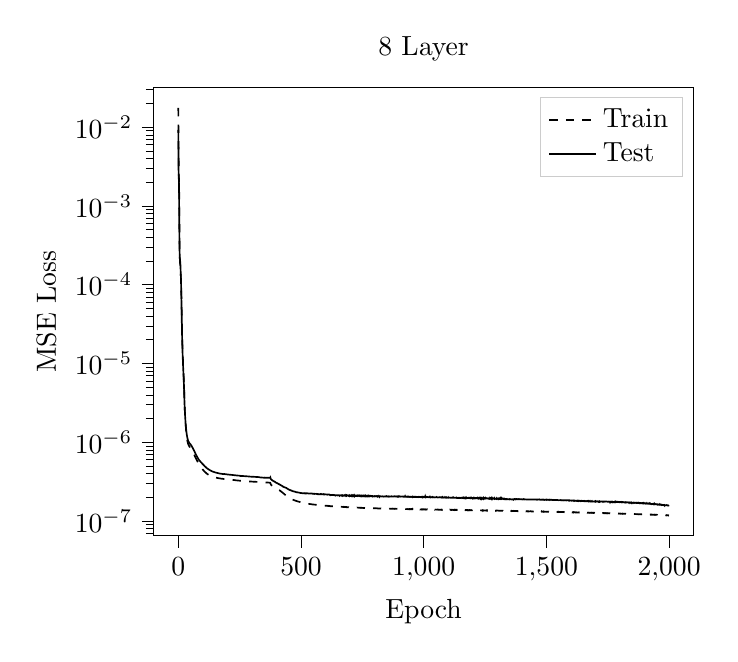
\begin{tikzpicture}

\begin{axis}[
legend cell align={left},
legend style={fill opacity=0.8, draw opacity=1, text opacity=1, draw=white!80!black},
log basis y={10},
tick align=outside,
tick pos=left,
title={8 Layer},
x grid style={white!69.0196078431373!black},
xlabel={Epoch},
xmin=-99.95, xmax=2098.95,
xtick style={color=black},
y grid style={white!69.0196078431373!black},
ylabel={MSE Loss},
ymin=6.47765029335508e-08, ymax=0.0318082202477323,
ymode=log,
ytick style={color=black}
]
\addplot [semithick, black, dashed]
table {%
0 0.0175328296050429
1 0.00526908103376627
2 0.0024811453698203
3 0.0020657035713084
4 0.00106903264287394
5 0.000353904425603105
6 0.000218746372745954
7 0.000189798295497894
8 0.000178016446661786
9 0.000159623949104571
10 0.000136344930841005
11 0.000113073929911479
12 8.84419990870811e-05
13 6.2893814065319e-05
14 4.27583082764613e-05
15 2.92383841242554e-05
16 2.10352017566038e-05
17 1.61476924668023e-05
18 1.30475415135152e-05
19 1.08516150257856e-05
20 9.16441520030276e-06
21 7.80614999439422e-06
22 6.68636070122375e-06
23 5.67973846887071e-06
24 4.59834968637551e-06
25 3.55384452848284e-06
26 2.82646348415483e-06
27 2.36879455329131e-06
28 2.06056119333198e-06
29 1.83083022565711e-06
30 1.64863851436792e-06
31 1.50096731364613e-06
32 1.38044920056757e-06
33 1.28160291140489e-06
34 1.20055532232755e-06
35 1.13477372232751e-06
36 1.08220113452262e-06
37 1.03955213090501e-06
38 1.00530486443517e-06
39 9.77610424797604e-07
40 9.54024540931186e-07
41 9.35144095763008e-07
42 9.20161763190208e-07
43 9.06661032530565e-07
44 8.95124449471041e-07
45 8.84884205675007e-07
46 8.75485176464963e-07
47 8.67158681160163e-07
48 8.58861131064259e-07
49 8.49627589815327e-07
50 8.40432371091993e-07
51 8.30126947960252e-07
52 8.20814274163695e-07
53 8.11791434074394e-07
54 8.02703816390249e-07
55 7.93062617361784e-07
56 7.83371090648188e-07
57 7.73359274489849e-07
58 7.63606251297233e-07
59 7.53800127654358e-07
60 7.43594718784379e-07
61 7.33601759947078e-07
62 7.23426322423393e-07
63 7.13205591125643e-07
64 7.0250906480851e-07
65 6.91736627373984e-07
66 6.8141382240583e-07
67 6.70850326486061e-07
68 6.60704809689605e-07
69 6.50622080343055e-07
70 6.40856266045375e-07
71 6.30526041106805e-07
72 6.21069840335053e-07
73 6.12328547347829e-07
74 6.03472821694595e-07
75 5.94954458605912e-07
76 5.86979994452008e-07
77 5.79193048764637e-07
78 5.7177413894749e-07
79 5.64665561554989e-07
80 5.5709349710753e-07
81 5.49923466209634e-07
82 5.4292612233553e-07
83 5.36258046594185e-07
84 5.29824090421016e-07
85 5.23648571146396e-07
86 5.17685902934772e-07
87 5.11069741804704e-07
88 5.05491432136296e-07
89 5.00108199872784e-07
90 4.9472347799906e-07
91 4.89829184886048e-07
92 4.84885792644718e-07
93 4.79588366886219e-07
94 4.74725679453059e-07
95 4.70136502784158e-07
96 4.65507118178721e-07
97 4.61073159385705e-07
98 4.56837894091677e-07
99 4.52725050351432e-07
100 4.48878952340692e-07
101 4.45040633863414e-07
102 4.41461416315292e-07
103 4.3791901580903e-07
104 4.34556433205557e-07
105 4.31228226531744e-07
106 4.28184232518447e-07
107 4.25006038128117e-07
108 4.22162241264346e-07
109 4.19006269950728e-07
110 4.16332390557272e-07
111 4.13429551699096e-07
112 4.10771487253214e-07
113 4.07942185475463e-07
114 4.05494348484581e-07
115 4.02784749738316e-07
116 4.00286914086223e-07
117 3.97965309545611e-07
118 3.95838657212266e-07
119 3.94044673285521e-07
120 3.92032634195516e-07
121 3.89872294590532e-07
122 3.88192757952766e-07
123 3.86300660608185e-07
124 3.84687878252521e-07
125 3.82859825634796e-07
126 3.81259326559302e-07
127 3.79667921393434e-07
128 3.7808499344294e-07
129 3.76785870017216e-07
130 3.75500086406078e-07
131 3.74170697980958e-07
132 3.72888158608475e-07
133 3.71877083168215e-07
134 3.70665013264215e-07
135 3.69590087345273e-07
136 3.68685641021216e-07
137 3.67684927169876e-07
138 3.66738080046503e-07
139 3.65638564375104e-07
140 3.64869017559499e-07
141 3.63847870005429e-07
142 3.62878456101612e-07
143 3.6201422052784e-07
144 3.61405104754908e-07
145 3.60622909369113e-07
146 3.59861233491188e-07
147 3.59144117268784e-07
148 3.58545277876487e-07
149 3.57887540502588e-07
150 3.57249293870154e-07
151 3.56527215444658e-07
152 3.56127539916429e-07
153 3.55544571846167e-07
154 3.55036048958368e-07
155 3.54611293843732e-07
156 3.54111535571633e-07
157 3.53505102594909e-07
158 3.52848333747602e-07
159 3.52149421956938e-07
160 3.51732665635041e-07
161 3.51205987101366e-07
162 3.50830501929522e-07
163 3.50395613395449e-07
164 3.49923345510206e-07
165 3.49431554028001e-07
166 3.48941883544285e-07
167 3.48522583536237e-07
168 3.48186346826651e-07
169 3.47681064312155e-07
170 3.47169353645427e-07
171 3.46804226069253e-07
172 3.46499707390535e-07
173 3.46075071732344e-07
174 3.45697041879589e-07
175 3.45525421082016e-07
176 3.45072367338162e-07
177 3.44646222188771e-07
178 3.44242588923294e-07
179 3.43962912864981e-07
180 3.43637114866624e-07
181 3.43373919974965e-07
182 3.43108959057759e-07
183 3.42715657879467e-07
184 3.42481556671714e-07
185 3.42151080772624e-07
186 3.41881741704242e-07
187 3.41519302025972e-07
188 3.41339824942111e-07
189 3.41067975909937e-07
190 3.4067830320339e-07
191 3.40474474853636e-07
192 3.40126796245954e-07
193 3.39870608186743e-07
194 3.39526693821313e-07
195 3.39317672114703e-07
196 3.38837426596683e-07
197 3.38705993669919e-07
198 3.38400550219831e-07
199 3.38316658016424e-07
200 3.37989257033655e-07
201 3.37688488230015e-07
202 3.37399379517933e-07
203 3.37125496955082e-07
204 3.36861192039351e-07
205 3.36608914466296e-07
206 3.36245998028062e-07
207 3.36085985836121e-07
208 3.35786493664614e-07
209 3.35561873896495e-07
210 3.35280411874805e-07
211 3.35142199233474e-07
212 3.34837603901406e-07
213 3.34593124080129e-07
214 3.34344883739845e-07
215 3.34137826051517e-07
216 3.33863607160367e-07
217 3.33455762159929e-07
218 3.3319723637959e-07
219 3.33105943873591e-07
220 3.32865009873728e-07
221 3.3264331553795e-07
222 3.32412592904063e-07
223 3.32070278993513e-07
224 3.31828170644144e-07
225 3.31597699712916e-07
226 3.31352910691862e-07
227 3.31146232390722e-07
228 3.31056747498337e-07
229 3.30603054095491e-07
230 3.30301297225333e-07
231 3.30080206424554e-07
232 3.29558580105527e-07
233 3.2933908271815e-07
234 3.29115459202001e-07
235 3.28839234775558e-07
236 3.28580431173009e-07
237 3.28323732759372e-07
238 3.2807043584171e-07
239 3.27747669892631e-07
240 3.27464948348677e-07
241 3.27200872433764e-07
242 3.26998274999823e-07
243 3.26803397669551e-07
244 3.26481064050199e-07
245 3.26303489700308e-07
246 3.26089179225164e-07
247 3.25924068953043e-07
248 3.25714338714533e-07
249 3.25468668862072e-07
250 3.25018146298817e-07
251 3.24853583165918e-07
252 3.24682733442216e-07
253 3.24474176309764e-07
254 3.24312471967403e-07
255 3.24107295426757e-07
256 3.23898819900137e-07
257 3.23801022510395e-07
258 3.23574237739876e-07
259 3.23386136919623e-07
260 3.23154673509407e-07
261 3.22951625179257e-07
262 3.22757495133885e-07
263 3.22559811543499e-07
264 3.22383646050639e-07
265 3.22176338926283e-07
266 3.21986999956891e-07
267 3.21799536330047e-07
268 3.21615479748516e-07
269 3.2131524605461e-07
270 3.21098087837868e-07
271 3.20949953959371e-07
272 3.20814928393531e-07
273 3.20597945510315e-07
274 3.20427085533481e-07
275 3.20249152103713e-07
276 3.2012393730696e-07
277 3.1993017118026e-07
278 3.19784813910928e-07
279 3.19583986197358e-07
280 3.1947266468535e-07
281 3.19318750968023e-07
282 3.19150666001633e-07
283 3.18975156424983e-07
284 3.18834318278505e-07
285 3.18683478894854e-07
286 3.18506897286852e-07
287 3.1842577485719e-07
288 3.18197053516656e-07
289 3.18177214133186e-07
290 3.17996098942785e-07
291 3.1795230303544e-07
292 3.17774085651479e-07
293 3.17555649353096e-07
294 3.17525105934635e-07
295 3.17360777685849e-07
296 3.17117739221828e-07
297 3.17186909256861e-07
298 3.16859379964285e-07
299 3.16811100702807e-07
300 3.16564827016919e-07
301 3.16546802324069e-07
302 3.16414311839708e-07
303 3.16191319463144e-07
304 3.16013029326712e-07
305 3.15986825370374e-07
306 3.1582280825404e-07
307 3.1556253458831e-07
308 3.15551690242444e-07
309 3.15488802044683e-07
310 3.15251602359012e-07
311 3.1524402550076e-07
312 3.14834048296575e-07
313 3.1502463754407e-07
314 3.14750351606108e-07
315 3.14771214370069e-07
316 3.1452549758626e-07
317 3.14477254761414e-07
318 3.14290501833625e-07
319 3.14295230836592e-07
320 3.13890693590224e-07
321 3.14136570423784e-07
322 3.1390767691164e-07
323 3.13873346939886e-07
324 3.13628105161001e-07
325 3.136031422315e-07
326 3.13384845625819e-07
327 3.13368351783083e-07
328 3.13223696586817e-07
329 3.13095284589338e-07
330 3.13103127901115e-07
331 3.12966587756591e-07
332 3.12709218896146e-07
333 3.12110520169995e-07
334 3.12222397674589e-07
335 3.12361991092303e-07
336 3.12118241708959e-07
337 3.11978893279274e-07
338 3.11915353471193e-07
339 3.11790699221604e-07
340 3.11596081047583e-07
341 3.11180611667794e-07
342 3.11583242257996e-07
343 3.11007668919672e-07
344 3.10850106806981e-07
345 3.10863525172067e-07
346 3.10767936177569e-07
347 3.10908169538493e-07
348 3.10390755146273e-07
349 3.10416143840087e-07
350 3.10616684522813e-07
351 3.10328716629726e-07
352 3.0965765838431e-07
353 3.09850993204464e-07
354 3.09702653474631e-07
355 3.09501027999204e-07
356 3.09061599175209e-07
357 3.09046005845914e-07
358 3.08902529347677e-07
359 3.08754219012997e-07
360 3.08652673965071e-07
361 3.0852893022626e-07
362 3.08412155753501e-07
363 3.08110915753446e-07
364 3.08090832113805e-07
365 3.07928383392664e-07
366 3.07783716692711e-07
367 3.07759822206322e-07
368 3.07536354554827e-07
369 3.07389559360161e-07
370 3.0712789580889e-07
371 3.07107941253548e-07
372 3.06821632392484e-07
373 3.06744424726446e-07
374 3.06417181519691e-07
375 3.05259786543388e-07
376 2.96313256789915e-07
377 2.90663783623302e-07
378 2.87804450067597e-07
379 2.85735052990788e-07
380 2.84615552835987e-07
381 2.83525199733958e-07
382 2.82446022225713e-07
383 2.81321543695867e-07
384 2.80254445300443e-07
385 2.7920743795562e-07
386 2.78225404251486e-07
387 2.77090234497734e-07
388 2.76221330814508e-07
389 2.75151829292497e-07
390 2.74080892651796e-07
391 2.72749642924452e-07
392 2.71503182730726e-07
393 2.70786939665868e-07
394 2.69418694927026e-07
395 2.68065543103546e-07
396 2.66677770433432e-07
397 2.65513972514952e-07
398 2.64282750272571e-07
399 2.62921956583284e-07
400 2.61887793861604e-07
401 2.60402524808967e-07
402 2.59187077418233e-07
403 2.58047188673061e-07
404 2.56683215951625e-07
405 2.55712748042924e-07
406 2.54107455099017e-07
407 2.53149617108761e-07
408 2.51396610721599e-07
409 2.50224179580982e-07
410 2.48511859005873e-07
411 2.47515977186197e-07
412 2.46467274273243e-07
413 2.44899058344572e-07
414 2.43662102086262e-07
415 2.42160927925283e-07
416 2.40837991377418e-07
417 2.39876552527107e-07
418 2.38471986328648e-07
419 2.36897201752129e-07
420 2.35599923733787e-07
421 2.34318138772949e-07
422 2.33158340222417e-07
423 2.31924687582818e-07
424 2.30379069428466e-07
425 2.29331601715899e-07
426 2.27478731481767e-07
427 2.26122672451368e-07
428 2.24842304703543e-07
429 2.23502054168989e-07
430 2.22350452716569e-07
431 2.21158989312187e-07
432 2.19953135321305e-07
433 2.18591989678885e-07
434 2.16939178685038e-07
435 2.15723278444102e-07
436 2.14631776202623e-07
437 2.13478038858739e-07
438 2.12388505580918e-07
439 2.11266726964254e-07
440 2.10094492594237e-07
441 2.08973344783203e-07
442 2.07528438195936e-07
443 2.06402683680551e-07
444 2.05239006199065e-07
445 2.04158008912714e-07
446 2.03251472335353e-07
447 2.02277326174283e-07
448 2.01125351324549e-07
449 2.00188082445152e-07
450 1.9919553130876e-07
451 1.98251505693747e-07
452 1.97417034669911e-07
453 1.96545381626834e-07
454 1.95746966497268e-07
455 1.95005100252388e-07
456 1.93978864757582e-07
457 1.93105879425559e-07
458 1.92514951393719e-07
459 1.91637039471004e-07
460 1.91000602328018e-07
461 1.90360802442058e-07
462 1.89602468800842e-07
463 1.89031795891026e-07
464 1.88446840532208e-07
465 1.87698710270467e-07
466 1.8711253670034e-07
467 1.86705542979837e-07
468 1.85847889987656e-07
469 1.855395490864e-07
470 1.85050495815631e-07
471 1.84422059135159e-07
472 1.837856653637e-07
473 1.83335924596406e-07
474 1.83027025578042e-07
475 1.82589353933338e-07
476 1.81720964455678e-07
477 1.81346602587951e-07
478 1.81113202692984e-07
479 1.80203582523575e-07
480 1.79770764276554e-07
481 1.79706625317522e-07
482 1.78981122033406e-07
483 1.78752520575642e-07
484 1.78582334385169e-07
485 1.77953864849201e-07
486 1.7766869345337e-07
487 1.77351471293719e-07
488 1.76812875736232e-07
489 1.76556565875785e-07
490 1.76516398234128e-07
491 1.76013626244753e-07
492 1.7571760091073e-07
493 1.75353105042575e-07
494 1.74835665283979e-07
495 1.74467691770985e-07
496 1.74291843606511e-07
497 1.7402895901597e-07
498 1.73773440145908e-07
499 1.73715644010031e-07
500 1.73122979084894e-07
501 1.73010420141395e-07
502 1.72502875500413e-07
503 1.72614680799654e-07
504 1.71815977353162e-07
505 1.71901242822514e-07
506 1.71326538904282e-07
507 1.71125863118959e-07
508 1.70994126413859e-07
509 1.70700766794596e-07
510 1.70445046293821e-07
511 1.70266769387695e-07
512 1.69651767969015e-07
513 1.69802070438152e-07
514 1.69355803713245e-07
515 1.69238175175224e-07
516 1.68864305237548e-07
517 1.68296895914466e-07
518 1.68144741152787e-07
519 1.681063232013e-07
520 1.67698545745054e-07
521 1.6727549429163e-07
522 1.67204165720136e-07
523 1.67013722361276e-07
524 1.66806940001152e-07
525 1.66711445601209e-07
526 1.66490661499097e-07
527 1.66064463151372e-07
528 1.6587639635901e-07
529 1.65645136902981e-07
530 1.65257467664048e-07
531 1.65194258968882e-07
532 1.65328429034162e-07
533 1.64852689202633e-07
534 1.64676807820285e-07
535 1.64541102527949e-07
536 1.64355891499213e-07
537 1.64472924332415e-07
538 1.64135093967843e-07
539 1.63986125564008e-07
540 1.63920706143017e-07
541 1.63486246314903e-07
542 1.63418712652685e-07
543 1.63100584771314e-07
544 1.63160991775158e-07
545 1.62823282899183e-07
546 1.62788972254191e-07
547 1.62310552298095e-07
548 1.62172701934082e-07
549 1.62233308088844e-07
550 1.62097987320919e-07
551 1.62025860142023e-07
552 1.61937730943862e-07
553 1.61551917692293e-07
554 1.6153179684153e-07
555 1.61515838158266e-07
556 1.61437829063971e-07
557 1.61197373074629e-07
558 1.61119178898161e-07
559 1.60824594509279e-07
560 1.60852694385483e-07
561 1.60977125005957e-07
562 1.60644661761467e-07
563 1.60562388401786e-07
564 1.60366760141528e-07
565 1.59942062417429e-07
566 1.59711742838908e-07
567 1.60133456724054e-07
568 1.59939134938725e-07
569 1.59850393622207e-07
570 1.59567545566119e-07
571 1.5941060387803e-07
572 1.59075994730529e-07
573 1.59110882194113e-07
574 1.59025825482217e-07
575 1.59193930166168e-07
576 1.59029426406221e-07
577 1.58960345970627e-07
578 1.58873228158996e-07
579 1.58691118166132e-07
580 1.58621524001035e-07
581 1.58440931521397e-07
582 1.5861286637886e-07
583 1.5840617636087e-07
584 1.58177897191081e-07
585 1.5795649078143e-07
586 1.57878831743119e-07
587 1.578905943731e-07
588 1.57640723230656e-07
589 1.57597480061611e-07
590 1.57342908707392e-07
591 1.56953609554478e-07
592 1.57225426349328e-07
593 1.57105286575643e-07
594 1.56963763622286e-07
595 1.56657359909218e-07
596 1.57128599077794e-07
597 1.56802190403482e-07
598 1.56697919422299e-07
599 1.5667860949975e-07
600 1.56515884235375e-07
601 1.56620291136278e-07
602 1.56279259520886e-07
603 1.56165708197875e-07
604 1.56020669244583e-07
605 1.56240268331942e-07
606 1.55817373048706e-07
607 1.56074017709784e-07
608 1.55637327125646e-07
609 1.5567520441806e-07
610 1.55283701715803e-07
611 1.55519019358508e-07
612 1.55492841116711e-07
613 1.55816570945433e-07
614 1.55335301293746e-07
615 1.55531510671381e-07
616 1.5507815454896e-07
617 1.55146671936279e-07
618 1.54875967719903e-07
619 1.53894253887898e-07
620 1.54305659787468e-07
621 1.54376400409717e-07
622 1.54427602577556e-07
623 1.54235710120076e-07
624 1.54084096209317e-07
625 1.54209941705119e-07
626 1.54026973827825e-07
627 1.54299684020032e-07
628 1.54060457653316e-07
629 1.54000254806164e-07
630 1.5397262653849e-07
631 1.5366859639343e-07
632 1.53862857217746e-07
633 1.53386126168442e-07
634 1.53348138315579e-07
635 1.53683566633589e-07
636 1.5352609095487e-07
637 1.53591393573294e-07
638 1.53002734407437e-07
639 1.5306999547704e-07
640 1.53088535963519e-07
641 1.53293578804892e-07
642 1.52966675685207e-07
643 1.52825601404061e-07
644 1.52772602113771e-07
645 1.52778851997937e-07
646 1.52619541619714e-07
647 1.52712212376116e-07
648 1.52516884270426e-07
649 1.52460694920364e-07
650 1.52448910270664e-07
651 1.52357230309264e-07
652 1.5242117907377e-07
653 1.5209905985003e-07
654 1.52307755726611e-07
655 1.52082216018812e-07
656 1.51867642628645e-07
657 1.52324002300475e-07
658 1.52034879739915e-07
659 1.52062457324575e-07
660 1.51832796557727e-07
661 1.51821761832593e-07
662 1.51722176934044e-07
663 1.51759662635698e-07
664 1.51708611028312e-07
665 1.51362560121271e-07
666 1.5133446582638e-07
667 1.51380364613374e-07
668 1.51449823185601e-07
669 1.51108101338338e-07
670 1.51180538388473e-07
671 1.50782916211512e-07
672 1.51165991443492e-07
673 1.51214464580107e-07
674 1.51761085135149e-07
675 1.50811644701321e-07
676 1.51023055781963e-07
677 1.50726220645936e-07
678 1.5102750061402e-07
679 1.50759341906337e-07
680 1.50863532468293e-07
681 1.5039412832607e-07
682 1.50405019361699e-07
683 1.50687183428033e-07
684 1.50395313138318e-07
685 1.49860707534089e-07
686 1.50543398369507e-07
687 1.49918052457565e-07
688 1.49921526016783e-07
689 1.50214154153616e-07
690 1.50098436261459e-07
691 1.49565287060227e-07
692 1.49665437476187e-07
693 1.50014687090305e-07
694 1.49929010170524e-07
695 1.49439825371189e-07
696 1.49774553186433e-07
697 1.49680220250303e-07
698 1.497078620325e-07
699 1.49463090451718e-07
700 1.49500760201704e-07
701 1.4965748385265e-07
702 1.49425968256622e-07
703 1.49092031882958e-07
704 1.49379718401121e-07
705 1.49784281770593e-07
706 1.49356223158037e-07
707 1.49130759467653e-07
708 1.48976830768532e-07
709 1.49068272978781e-07
710 1.49264540628025e-07
711 1.4917010704707e-07
712 1.49419977461207e-07
713 1.48736793999404e-07
714 1.48965444530802e-07
715 1.48944377855287e-07
716 1.49004637158612e-07
717 1.48904402827554e-07
718 1.48690500225257e-07
719 1.4850534645916e-07
720 1.48886191965403e-07
721 1.48935314744136e-07
722 1.48329525529789e-07
723 1.48342651343114e-07
724 1.48138873964143e-07
725 1.48427777201476e-07
726 1.48268044057431e-07
727 1.48134518688892e-07
728 1.48310625430526e-07
729 1.48065957461085e-07
730 1.48151556441434e-07
731 1.48060626877111e-07
732 1.4802541597092e-07
733 1.47803417629433e-07
734 1.4787964930818e-07
735 1.48006359665942e-07
736 1.4761687753051e-07
737 1.47693905873325e-07
738 1.47604845977867e-07
739 1.47512238822145e-07
740 1.47706481826049e-07
741 1.47676154170995e-07
742 1.46773032945191e-07
743 1.47055220313774e-07
744 1.47239715392544e-07
745 1.467912592652e-07
746 1.47049525299536e-07
747 1.47205613501455e-07
748 1.47109882039587e-07
749 1.4667980613936e-07
750 1.46820244534496e-07
751 1.46917181776729e-07
752 1.46934573837854e-07
753 1.46922250465309e-07
754 1.46629619326433e-07
755 1.46714902022893e-07
756 1.46811325457463e-07
757 1.46594789793397e-07
758 1.46552674767264e-07
759 1.46794158258245e-07
760 1.46406611559513e-07
761 1.46276465741835e-07
762 1.46520066905964e-07
763 1.46337387764817e-07
764 1.46368378977968e-07
765 1.46322530774512e-07
766 1.46444433365645e-07
767 1.46170982674221e-07
768 1.46035282174495e-07
769 1.46347738876784e-07
770 1.45868453255815e-07
771 1.45995072564631e-07
772 1.4621667817849e-07
773 1.45996149388594e-07
774 1.45838359781436e-07
775 1.46086144560797e-07
776 1.45816849595803e-07
777 1.45792429265157e-07
778 1.4566305859276e-07
779 1.46017009416966e-07
780 1.45877792149918e-07
781 1.45809088923698e-07
782 1.45412859740901e-07
783 1.45728202642914e-07
784 1.45793485817336e-07
785 1.45572990955856e-07
786 1.45507330024941e-07
787 1.45483349449194e-07
788 1.45378579937017e-07
789 1.45243717270205e-07
790 1.45138936225919e-07
791 1.45445496556817e-07
792 1.4537288086558e-07
793 1.45323052233692e-07
794 1.45249136412673e-07
795 1.44959458381777e-07
796 1.45310082043437e-07
797 1.45089904361129e-07
798 1.44886737540872e-07
799 1.45202101947461e-07
800 1.45081607684006e-07
801 1.45068235003265e-07
802 1.45047729315451e-07
803 1.44639789915857e-07
804 1.44681112377754e-07
805 1.45097899459046e-07
806 1.44912972412925e-07
807 1.44757418407693e-07
808 1.44969247070748e-07
809 1.44877304595781e-07
810 1.45066319774401e-07
811 1.44526176367066e-07
812 1.44770261883309e-07
813 1.44676769728846e-07
814 1.44596687665199e-07
815 1.44527480813394e-07
816 1.44417752558468e-07
817 1.44684981730592e-07
818 1.44646610436894e-07
819 1.44546390689726e-07
820 1.44043759831902e-07
821 1.43988481575263e-07
822 1.44454864035026e-07
823 1.44367983928362e-07
824 1.44315122295069e-07
825 1.44514851303512e-07
826 1.44211226373869e-07
827 1.44078816024518e-07
828 1.44293243820925e-07
829 1.44206716939266e-07
830 1.44275118252324e-07
831 1.44198291060604e-07
832 1.43960377940289e-07
833 1.44308390385817e-07
834 1.43741077277326e-07
835 1.43910124183577e-07
836 1.44126620742924e-07
837 1.44111164065208e-07
838 1.4420608047061e-07
839 1.43975314230715e-07
840 1.44012661287718e-07
841 1.43980029530866e-07
842 1.43928399559456e-07
843 1.43848968185978e-07
844 1.43690816585718e-07
845 1.44003668232529e-07
846 1.43679508973094e-07
847 1.43783171800749e-07
848 1.43928508908431e-07
849 1.43680912799482e-07
850 1.44121392462893e-07
851 1.43895006939232e-07
852 1.43512517407629e-07
853 1.43355135772794e-07
854 1.43424258631342e-07
855 1.43617109703342e-07
856 1.43774829503229e-07
857 1.43508643439816e-07
858 1.43625492381005e-07
859 1.43168517407588e-07
860 1.43556524633937e-07
861 1.43369579628683e-07
862 1.4350661416529e-07
863 1.43150451556551e-07
864 1.43568707436259e-07
865 1.4335619835748e-07
866 1.43229341304618e-07
867 1.43312628949843e-07
868 1.43442354200829e-07
869 1.43290071264346e-07
870 1.43341870831648e-07
871 1.43120179540546e-07
872 1.43148483605415e-07
873 1.42917345435478e-07
874 1.43662633611541e-07
875 1.42980072517673e-07
876 1.42999039763225e-07
877 1.43008041625592e-07
878 1.43002305986073e-07
879 1.43241044330722e-07
880 1.42978790144355e-07
881 1.43165590785088e-07
882 1.42598846199604e-07
883 1.43180287722089e-07
884 1.42780469488457e-07
885 1.42780916569052e-07
886 1.42969993397912e-07
887 1.42703800605659e-07
888 1.42895849410962e-07
889 1.42793996602109e-07
890 1.42831420259171e-07
891 1.42718856707802e-07
892 1.42954531902717e-07
893 1.42701163781567e-07
894 1.42444937743846e-07
895 1.4261761233314e-07
896 1.42605217273939e-07
897 1.42689636913218e-07
898 1.42392338929653e-07
899 1.4255365073268e-07
900 1.42336699212819e-07
901 1.42699972283111e-07
902 1.42488840616295e-07
903 1.4252937375403e-07
904 1.4202959576437e-07
905 1.425743420711e-07
906 1.4243057094987e-07
907 1.42474533404879e-07
908 1.42089733259354e-07
909 1.42119609343183e-07
910 1.42345393491894e-07
911 1.42107149244453e-07
912 1.42211034706463e-07
913 1.4240851080416e-07
914 1.4221744854126e-07
915 1.42267661875195e-07
916 1.42202555696969e-07
917 1.41925924797448e-07
918 1.41971158406307e-07
919 1.4210136470183e-07
920 1.42300199058809e-07
921 1.4193852898714e-07
922 1.42140022891368e-07
923 1.42676953529985e-07
924 1.42855565659517e-07
925 1.42496458355623e-07
926 1.42077827710807e-07
927 1.4173500014536e-07
928 1.41774210817402e-07
929 1.4185019106705e-07
930 1.41530856794247e-07
931 1.41516090682359e-07
932 1.4148874922526e-07
933 1.41717627791138e-07
934 1.41738756664012e-07
935 1.42321595205885e-07
936 1.41502772880386e-07
937 1.41590681753456e-07
938 1.4135556979511e-07
939 1.41424335893703e-07
940 1.4142615881596e-07
941 1.42026300974152e-07
942 1.41953662016192e-07
943 1.41265155992443e-07
944 1.42225362758097e-07
945 1.4185230777386e-07
946 1.4118388476092e-07
947 1.41045869781919e-07
948 1.40988311517987e-07
949 1.42108610312164e-07
950 1.42266998906848e-07
951 1.41178457901958e-07
952 1.40924142737475e-07
953 1.4084296048722e-07
954 1.41030333150383e-07
955 1.42312434267211e-07
956 1.40815855555587e-07
957 1.41811550495419e-07
958 1.41584311652565e-07
959 1.40938345623454e-07
960 1.40837006021854e-07
961 1.41598450394298e-07
962 1.41160173079413e-07
963 1.40844735707191e-07
964 1.41018507303414e-07
965 1.40989900536681e-07
966 1.41357851422441e-07
967 1.41701209749101e-07
968 1.40556913073908e-07
969 1.41622540972719e-07
970 1.40686534969348e-07
971 1.4053291606686e-07
972 1.40638144088712e-07
973 1.41467908843396e-07
974 1.40740276282969e-07
975 1.40685108373617e-07
976 1.40603891324531e-07
977 1.40684053398843e-07
978 1.41419389557029e-07
979 1.41598929936038e-07
980 1.41155748718091e-07
981 1.4127184632784e-07
982 1.41115515578605e-07
983 1.41157341086995e-07
984 1.41093482294963e-07
985 1.40244625491448e-07
986 1.40437968127571e-07
987 1.40473355934034e-07
988 1.40752477928885e-07
989 1.40687068828527e-07
990 1.40017776338652e-07
991 1.41015269630174e-07
992 1.40835331620792e-07
993 1.40545132662595e-07
994 1.41174887165363e-07
995 1.41119856710503e-07
996 1.40208206119041e-07
997 1.40931780023834e-07
998 1.4022020828719e-07
999 1.40919137169959e-07
1000 1.40721628962837e-07
1001 1.40827392534959e-07
1002 1.40272580253509e-07
1003 1.39982767475288e-07
1004 1.4001712857592e-07
1005 1.41045355317004e-07
1006 1.40934940986881e-07
1007 1.40801237918708e-07
1008 1.40705775212524e-07
1009 1.39573305421692e-07
1010 1.40005285206968e-07
1011 1.39985599552972e-07
1012 1.3998350164357e-07
1013 1.40217492749173e-07
1014 1.40933221167927e-07
1015 1.40469146966637e-07
1016 1.39870673319109e-07
1017 1.40242820979353e-07
1018 1.40717302322457e-07
1019 1.39738414247859e-07
1020 1.40684658493484e-07
1021 1.39640350049319e-07
1022 1.3976327009857e-07
1023 1.40896664014178e-07
1024 1.4003093021131e-07
1025 1.40633622720543e-07
1026 1.40413035932596e-07
1027 1.40312370913165e-07
1028 1.39787127331203e-07
1029 1.40090054060238e-07
1030 1.40548668227325e-07
1031 1.39413021557289e-07
1032 1.39588993896211e-07
1033 1.40005150228717e-07
1034 1.39753148697963e-07
1035 1.39596208203585e-07
1036 1.3951229968967e-07
1037 1.40408136896752e-07
1038 1.39835310108083e-07
1039 1.40405866954296e-07
1040 1.40260662099934e-07
1041 1.39776692630988e-07
1042 1.40046229791579e-07
1043 1.40275582459992e-07
1044 1.39946306664029e-07
1045 1.39301153780025e-07
1046 1.39497414391343e-07
1047 1.39598235257665e-07
1048 1.39690142994198e-07
1049 1.39807074788223e-07
1050 1.39737415786101e-07
1051 1.39700335019199e-07
1052 1.39594883965088e-07
1053 1.3950548950703e-07
1054 1.39740799987464e-07
1055 1.39295418208008e-07
1056 1.3973811096335e-07
1057 1.40247204662103e-07
1058 1.39764830574762e-07
1059 1.39799569627286e-07
1060 1.39192969097479e-07
1061 1.39496986072629e-07
1062 1.39270260721247e-07
1063 1.39414751853195e-07
1064 1.39368439160847e-07
1065 1.39430535600837e-07
1066 1.39370543582373e-07
1067 1.39014138344606e-07
1068 1.3903848970287e-07
1069 1.39036954866611e-07
1070 1.38956512998334e-07
1071 1.39268774670853e-07
1072 1.39314872974694e-07
1073 1.38759399373356e-07
1074 1.3974047739751e-07
1075 1.38765189806378e-07
1076 1.39840884134657e-07
1077 1.39689777260088e-07
1078 1.3940588398853e-07
1079 1.39469934833159e-07
1080 1.39180955024187e-07
1081 1.3941563042863e-07
1082 1.38784151552329e-07
1083 1.39607714665146e-07
1084 1.38701271541919e-07
1085 1.39057623346872e-07
1086 1.39424572637381e-07
1087 1.39112138135999e-07
1088 1.38356904830772e-07
1089 1.38704682374424e-07
1090 1.39570322634341e-07
1091 1.39438522612778e-07
1092 1.39256844970959e-07
1093 1.38886850859166e-07
1094 1.39106300593994e-07
1095 1.38832809213341e-07
1096 1.38724195892337e-07
1097 1.38557934619143e-07
1098 1.39467144848027e-07
1099 1.39032704108644e-07
1100 1.38914165511039e-07
1101 1.39027073945641e-07
1102 1.386054461463e-07
1103 1.3844797469531e-07
1104 1.38298065451181e-07
1105 1.38539775452529e-07
1106 1.38387163005405e-07
1107 1.39363646990631e-07
1108 1.39057628707917e-07
1109 1.3864583001677e-07
1110 1.38458758947024e-07
1111 1.38663611714662e-07
1112 1.38217955239384e-07
1113 1.39053501012398e-07
1114 1.38698975955975e-07
1115 1.38392806523058e-07
1116 1.38454945290079e-07
1117 1.38877848510077e-07
1118 1.38484777625791e-07
1119 1.3804813632845e-07
1120 1.384317418065e-07
1121 1.38236011867576e-07
1122 1.38729906922208e-07
1123 1.3860993410475e-07
1124 1.38744956498016e-07
1125 1.37916542406913e-07
1126 1.39003695924345e-07
1127 1.38235406847542e-07
1128 1.38581443195562e-07
1129 1.38985475299336e-07
1130 1.38347661192029e-07
1131 1.3873075161186e-07
1132 1.38244267315457e-07
1133 1.38409569611753e-07
1134 1.38766601232021e-07
1135 1.3816313969528e-07
1136 1.3874601235031e-07
1137 1.38215914162743e-07
1138 1.38433437424368e-07
1139 1.38305761815616e-07
1140 1.3816990382054e-07
1141 1.38154227816045e-07
1142 1.3817131157623e-07
1143 1.37816663091428e-07
1144 1.37279932747703e-07
1145 1.38278222902244e-07
1146 1.38441186155802e-07
1147 1.38293754037733e-07
1148 1.38114186285065e-07
1149 1.38382457134156e-07
1150 1.38121935648883e-07
1151 1.38317404871913e-07
1152 1.3726398281122e-07
1153 1.38135500790781e-07
1154 1.37828834432696e-07
1155 1.37260662473437e-07
1156 1.37698246579276e-07
1157 1.38406393155321e-07
1158 1.38022530450144e-07
1159 1.38276047778163e-07
1160 1.37411542546317e-07
1161 1.38349900112189e-07
1162 1.37902236627241e-07
1163 1.38121288390636e-07
1164 1.37785931336509e-07
1165 1.38097032252205e-07
1166 1.38174561051585e-07
1167 1.38032484766626e-07
1168 1.37848963614573e-07
1169 1.3723605952265e-07
1170 1.37956863941469e-07
1171 1.37981708157042e-07
1172 1.37641746089656e-07
1173 1.37537446441627e-07
1174 1.37715307477748e-07
1175 1.3802467366375e-07
1176 1.37435121121854e-07
1177 1.37773701698762e-07
1178 1.37598071777489e-07
1179 1.37826937510965e-07
1180 1.3687629511594e-07
1181 1.3763023151725e-07
1182 1.37472484304624e-07
1183 1.36806704883696e-07
1184 1.37347097012963e-07
1185 1.36806844061255e-07
1186 1.37831803662891e-07
1187 1.37434617570875e-07
1188 1.3769349364523e-07
1189 1.37824878567727e-07
1190 1.37278291237664e-07
1191 1.37285638022178e-07
1192 1.37537405553445e-07
1193 1.37367708799019e-07
1194 1.37173955799597e-07
1195 1.3737849220874e-07
1196 1.37694570426561e-07
1197 1.37204371121413e-07
1198 1.37134707571818e-07
1199 1.37665647152119e-07
1200 1.36953320932776e-07
1201 1.37370643354728e-07
1202 1.37206181204164e-07
1203 1.37008231114066e-07
1204 1.37595916893218e-07
1205 1.36808668081301e-07
1206 1.37278483379077e-07
1207 1.37148173621426e-07
1208 1.37073568943435e-07
1209 1.36834813723397e-07
1210 1.37074007465543e-07
1211 1.37088900583393e-07
1212 1.37079231969039e-07
1213 1.36705124127445e-07
1214 1.37048769406789e-07
1215 1.37013939077946e-07
1216 1.37600832001539e-07
1217 1.36949269979425e-07
1218 1.37130617353876e-07
1219 1.37060159055125e-07
1220 1.37085094007006e-07
1221 1.36812554405452e-07
1222 1.37024799300889e-07
1223 1.36926175436258e-07
1224 1.36370574427502e-07
1225 1.36324622825867e-07
1226 1.36892710990821e-07
1227 1.36951245121253e-07
1228 1.36814091263204e-07
1229 1.3654238679095e-07
1230 1.37057469043356e-07
1231 1.36701299577879e-07
1232 1.3652721672841e-07
1233 1.3685295296284e-07
1234 1.36608417133033e-07
1235 1.36408859674475e-07
1236 1.36091057672871e-07
1237 1.3619267259557e-07
1238 1.36285035583938e-07
1239 1.36530719178296e-07
1240 1.37105354312439e-07
1241 1.35431814818787e-07
1242 1.3684890741672e-07
1243 1.3663633738048e-07
1244 1.36236742655171e-07
1245 1.36506144674087e-07
1246 1.36222827489263e-07
1247 1.36451787916769e-07
1248 1.36626566039411e-07
1249 1.36391327373531e-07
1250 1.36479924456978e-07
1251 1.35830370680878e-07
1252 1.35618493807499e-07
1253 1.35934234069879e-07
1254 1.36055470630225e-07
1255 1.36669150702318e-07
1256 1.36405847417365e-07
1257 1.36319522386685e-07
1258 1.35291791945491e-07
1259 1.36776484112033e-07
1260 1.36283775297841e-07
1261 1.36266703815835e-07
1262 1.35965188928111e-07
1263 1.36535373140845e-07
1264 1.35733946944327e-07
1265 1.3617216602313e-07
1266 1.36112452828741e-07
1267 1.36237589192234e-07
1268 1.36063071604298e-07
1269 1.35476228248166e-07
1270 1.36250667537752e-07
1271 1.35881678090755e-07
1272 1.35979288831578e-07
1273 1.36238702118874e-07
1274 1.35648261981203e-07
1275 1.35880330763172e-07
1276 1.35914717418473e-07
1277 1.36027546457029e-07
1278 1.35853306886702e-07
1279 1.35285529214713e-07
1280 1.35539836794152e-07
1281 1.35683692555233e-07
1282 1.36025817489838e-07
1283 1.35835172550003e-07
1284 1.35056589666505e-07
1285 1.35935776850005e-07
1286 1.35621498060345e-07
1287 1.35414710101145e-07
1288 1.3520019967217e-07
1289 1.35646540183387e-07
1290 1.35784820663787e-07
1291 1.35338610498081e-07
1292 1.35329451261157e-07
1293 1.3545026487094e-07
1294 1.34593553923423e-07
1295 1.35693883191124e-07
1296 1.35603320561728e-07
1297 1.35862542691711e-07
1298 1.35825982674476e-07
1299 1.35838342881556e-07
1300 1.35632517498152e-07
1301 1.35736545058052e-07
1302 1.35440545069088e-07
1303 1.35403063097783e-07
1304 1.35380686813846e-07
1305 1.35425861454763e-07
1306 1.35607733412257e-07
1307 1.35032257166046e-07
1308 1.35039564661099e-07
1309 1.35352815490819e-07
1310 1.35184736461014e-07
1311 1.35230940468745e-07
1312 1.35324441441043e-07
1313 1.34647033465995e-07
1314 1.34791245049115e-07
1315 1.35218023384454e-07
1316 1.35195162897617e-07
1317 1.35294213944093e-07
1318 1.3488464167466e-07
1319 1.35344892409961e-07
1320 1.34881540162723e-07
1321 1.35190767682758e-07
1322 1.35402391805428e-07
1323 1.34437263884735e-07
1324 1.35373538814321e-07
1325 1.3493949830945e-07
1326 1.34989981521727e-07
1327 1.3497682837027e-07
1328 1.34721640101532e-07
1329 1.34469346654953e-07
1330 1.34818239921231e-07
1331 1.33841995442197e-07
1332 1.34700803222643e-07
1333 1.3439547620564e-07
1334 1.34984121679338e-07
1335 1.34795854503267e-07
1336 1.34525469743352e-07
1337 1.3461953422933e-07
1338 1.34462001998514e-07
1339 1.34843029677256e-07
1340 1.3420433430511e-07
1341 1.34563807471011e-07
1342 1.34867390901405e-07
1343 1.34510761792939e-07
1344 1.34730030342922e-07
1345 1.34435606849337e-07
1346 1.34411263609024e-07
1347 1.34256437316793e-07
1348 1.34782813972834e-07
1349 1.34024590582982e-07
1350 1.34568452995865e-07
1351 1.34362380514119e-07
1352 1.34302472829972e-07
1353 1.34351334761362e-07
1354 1.34335907890915e-07
1355 1.34120713873642e-07
1356 1.34727013193725e-07
1357 1.3408221532174e-07
1358 1.34729800823408e-07
1359 1.33871938110985e-07
1360 1.34318109189735e-07
1361 1.33864743343537e-07
1362 1.33782924415016e-07
1363 1.33831355135783e-07
1364 1.34113517070489e-07
1365 1.34292689914162e-07
1366 1.33977288928833e-07
1367 1.34500697772211e-07
1368 1.33883850152117e-07
1369 1.34232168132797e-07
1370 1.34191160224617e-07
1371 1.33971361943708e-07
1372 1.34148812882984e-07
1373 1.34059907523465e-07
1374 1.34011533003076e-07
1375 1.33912587273244e-07
1376 1.34207291516475e-07
1377 1.33993816298528e-07
1378 1.33813187630949e-07
1379 1.33925051226669e-07
1380 1.33609595302175e-07
1381 1.33904241835125e-07
1382 1.34056787935322e-07
1383 1.33134117795919e-07
1384 1.33370779437314e-07
1385 1.33212562847262e-07
1386 1.33458020300736e-07
1387 1.3342541274497e-07
1388 1.33344620042664e-07
1389 1.33045203249083e-07
1390 1.33173939648401e-07
1391 1.33735852706707e-07
1392 1.33101146182923e-07
1393 1.33628113918149e-07
1394 1.33048745031061e-07
1395 1.3363897600982e-07
1396 1.33286138424893e-07
1397 1.33129509002572e-07
1398 1.33416546312048e-07
1399 1.33238605958042e-07
1400 1.33379363671082e-07
1401 1.32978078468682e-07
1402 1.3356520895158e-07
1403 1.32921508672723e-07
1404 1.33823932376487e-07
1405 1.32866876739968e-07
1406 1.33234917843339e-07
1407 1.33153241058892e-07
1408 1.33098256689834e-07
1409 1.33156855461891e-07
1410 1.32817506489857e-07
1411 1.32931520688828e-07
1412 1.33269521125356e-07
1413 1.33011132493976e-07
1414 1.33485634137287e-07
1415 1.33242297888359e-07
1416 1.33132474370967e-07
1417 1.3259303654678e-07
1418 1.3304268214398e-07
1419 1.33466728897247e-07
1420 1.33002457850751e-07
1421 1.32801221386813e-07
1422 1.33324380179545e-07
1423 1.3274783855266e-07
1424 1.33157652172144e-07
1425 1.3254952354913e-07
1426 1.32873556612623e-07
1427 1.32407889910979e-07
1428 1.32744041508204e-07
1429 1.32378662826227e-07
1430 1.32670230499343e-07
1431 1.32587954393415e-07
1432 1.32656734994185e-07
1433 1.32849608920793e-07
1434 1.32743974827321e-07
1435 1.32634176555513e-07
1436 1.33182105667373e-07
1437 1.32471532481304e-07
1438 1.32415526973517e-07
1439 1.32673556713314e-07
1440 1.32404575865053e-07
1441 1.32716721562787e-07
1442 1.32429709207571e-07
1443 1.32324919132287e-07
1444 1.32314515127518e-07
1445 1.32301039705851e-07
1446 1.3211925281098e-07
1447 1.32657475521825e-07
1448 1.32912559909215e-07
1449 1.32554381384153e-07
1450 1.32347947413791e-07
1451 1.32099213207226e-07
1452 1.32150625326233e-07
1453 1.32160753622657e-07
1454 1.3207741969623e-07
1455 1.31980249019392e-07
1456 1.32116101994484e-07
1457 1.32137307879532e-07
1458 1.32061789404503e-07
1459 1.32048744411861e-07
1460 1.32378337653449e-07
1461 1.32101896774373e-07
1462 1.32699420056781e-07
1463 1.31930627890853e-07
1464 1.32252337969874e-07
1465 1.32622942700777e-07
1466 1.32286355036371e-07
1467 1.32539021823419e-07
1468 1.32651284406649e-07
1469 1.32340801513919e-07
1470 1.32256910539752e-07
1471 1.32004824102694e-07
1472 1.32280205178859e-07
1473 1.32093755226492e-07
1474 1.31662019260403e-07
1475 1.32213106066814e-07
1476 1.31271451138559e-07
1477 1.31864246128544e-07
1478 1.31608354905666e-07
1479 1.30965473260858e-07
1480 1.32271324694955e-07
1481 1.31262430571155e-07
1482 1.31543934809741e-07
1483 1.313864367809e-07
1484 1.31590168670925e-07
1485 1.31592009804393e-07
1486 1.32355213668944e-07
1487 1.31233894322236e-07
1488 1.322243186479e-07
1489 1.31188508561308e-07
1490 1.31564933301576e-07
1491 1.31285795003322e-07
1492 1.31731327115858e-07
1493 1.3135731555991e-07
1494 1.31512092288233e-07
1495 1.31611965763057e-07
1496 1.31706112298957e-07
1497 1.31114311969327e-07
1498 1.31415391560807e-07
1499 1.31099050221906e-07
1500 1.31427122809669e-07
1501 1.31453035884022e-07
1502 1.3128647963967e-07
1503 1.3111958820744e-07
1504 1.31147327294912e-07
1505 1.31227129489986e-07
1506 1.31290460291922e-07
1507 1.30941434587584e-07
1508 1.31656905814737e-07
1509 1.31472641921704e-07
1510 1.30588963141776e-07
1511 1.31188821065109e-07
1512 1.31706080967575e-07
1513 1.31110556782943e-07
1514 1.30758157158795e-07
1515 1.3106696122378e-07
1516 1.31225491454501e-07
1517 1.31034349763581e-07
1518 1.3103017726479e-07
1519 1.30969628866495e-07
1520 1.30797065246213e-07
1521 1.30787288117773e-07
1522 1.30791775951877e-07
1523 1.30976999024313e-07
1524 1.31051221554657e-07
1525 1.30748538129666e-07
1526 1.30839846438136e-07
1527 1.30894191624265e-07
1528 1.30849193311633e-07
1529 1.30806471442924e-07
1530 1.31186622411406e-07
1531 1.30813544863884e-07
1532 1.30370885592868e-07
1533 1.30964306318759e-07
1534 1.3051633526473e-07
1535 1.3060982085733e-07
1536 1.3062497325933e-07
1537 1.3089209088335e-07
1538 1.30859886741774e-07
1539 1.30665071250036e-07
1540 1.30388852678465e-07
1541 1.30435781791505e-07
1542 1.3038937690979e-07
1543 1.30548729455171e-07
1544 1.30223722596412e-07
1545 1.30463539424142e-07
1546 1.30992637611627e-07
1547 1.30539175991373e-07
1548 1.30286821075742e-07
1549 1.30969028202088e-07
1550 1.30108640519211e-07
1551 1.30534399804816e-07
1552 1.305582544191e-07
1553 1.30258834200703e-07
1554 1.30274908006101e-07
1555 1.30317872567787e-07
1556 1.30202957059566e-07
1557 1.30228620776052e-07
1558 1.30101475114941e-07
1559 1.30086796559681e-07
1560 1.30293293448602e-07
1561 1.2986444609453e-07
1562 1.3018359702599e-07
1563 1.30214615438717e-07
1564 1.29875511923672e-07
1565 1.29994600268191e-07
1566 1.3004828747043e-07
1567 1.29831804429159e-07
1568 1.30118920726119e-07
1569 1.2980349151448e-07
1570 1.30118059821882e-07
1571 1.30010312890505e-07
1572 1.29579943731528e-07
1573 1.30007581773839e-07
1574 1.29633749793356e-07
1575 1.30228536164623e-07
1576 1.30193649013677e-07
1577 1.29590583252792e-07
1578 1.29725245866297e-07
1579 1.30004574170783e-07
1580 1.29605912349007e-07
1581 1.30095143621389e-07
1582 1.29633200369739e-07
1583 1.29431262894997e-07
1584 1.29868774312314e-07
1585 1.29622148691055e-07
1586 1.29606173121743e-07
1587 1.29350665538652e-07
1588 1.29556376911921e-07
1589 1.29484209988817e-07
1590 1.29671797054698e-07
1591 1.29224490592605e-07
1592 1.29702454305658e-07
1593 1.29253210268132e-07
1594 1.29577081668941e-07
1595 1.29228094142064e-07
1596 1.29756646185086e-07
1597 1.29241407474723e-07
1598 1.29243841310966e-07
1599 1.29316493936216e-07
1600 1.29171331739286e-07
1601 1.29152005960975e-07
1602 1.29362774728747e-07
1603 1.29053464974049e-07
1604 1.2973606031963e-07
1605 1.28797939900949e-07
1606 1.292929365313e-07
1607 1.28868934151427e-07
1608 1.29265904050158e-07
1609 1.28977175595679e-07
1610 1.29510403507282e-07
1611 1.28456110278563e-07
1612 1.29433031272441e-07
1613 1.28712626203509e-07
1614 1.28916061377993e-07
1615 1.29057485636963e-07
1616 1.28958677031221e-07
1617 1.28673919501665e-07
1618 1.28923699293182e-07
1619 1.28449451679558e-07
1620 1.29111401921733e-07
1621 1.28495435795628e-07
1622 1.28987836760075e-07
1623 1.28698487564805e-07
1624 1.28473070812873e-07
1625 1.28501706306849e-07
1626 1.28262596685857e-07
1627 1.28696789822413e-07
1628 1.28623904696923e-07
1629 1.28384659472403e-07
1630 1.28826351435407e-07
1631 1.28461536736069e-07
1632 1.28665960101415e-07
1633 1.28115977716448e-07
1634 1.28646519687692e-07
1635 1.28333325623231e-07
1636 1.28468673370463e-07
1637 1.28419803250068e-07
1638 1.28151095964313e-07
1639 1.28518776765674e-07
1640 1.27761854844977e-07
1641 1.28458843533963e-07
1642 1.27842088506469e-07
1643 1.28688504545948e-07
1644 1.28137436067988e-07
1645 1.28033213929513e-07
1646 1.28139297540741e-07
1647 1.2777365060046e-07
1648 1.28386569663519e-07
1649 1.27739248984682e-07
1650 1.28065944082323e-07
1651 1.2789484215503e-07
1652 1.28238655840107e-07
1653 1.2774030926721e-07
1654 1.27987645285543e-07
1655 1.27901294991517e-07
1656 1.27665742937211e-07
1657 1.28034646415642e-07
1658 1.27770535438998e-07
1659 1.28071750069125e-07
1660 1.2736325490792e-07
1661 1.27776725353357e-07
1662 1.27459353095105e-07
1663 1.2781280282681e-07
1664 1.27549898106594e-07
1665 1.27953898388711e-07
1666 1.27458225748001e-07
1667 1.27477272538812e-07
1668 1.27502214869679e-07
1669 1.27840303445481e-07
1670 1.27344695510345e-07
1671 1.2779773659588e-07
1672 1.27378690098823e-07
1673 1.27423267638704e-07
1674 1.27738863163529e-07
1675 1.27728986679898e-07
1676 1.27057836525779e-07
1677 1.27538693256213e-07
1678 1.27737066165423e-07
1679 1.2724590301616e-07
1680 1.27389885889784e-07
1681 1.27419158154396e-07
1682 1.26930182634766e-07
1683 1.27623879183858e-07
1684 1.27154275617158e-07
1685 1.27618358977344e-07
1686 1.27124929791833e-07
1687 1.27371926229358e-07
1688 1.26812731377157e-07
1689 1.27139282056987e-07
1690 1.27218484401226e-07
1691 1.26683921443771e-07
1692 1.27419617534485e-07
1693 1.27127938714722e-07
1694 1.26770443650059e-07
1695 1.26936346060091e-07
1696 1.27238350650316e-07
1697 1.26644798047693e-07
1698 1.27171476734134e-07
1699 1.27158263339311e-07
1700 1.26667268503411e-07
1701 1.26758011871786e-07
1702 1.26943203177632e-07
1703 1.26554607881246e-07
1704 1.26810259747145e-07
1705 1.26932658776724e-07
1706 1.26421777608243e-07
1707 1.2673739819391e-07
1708 1.26697367846873e-07
1709 1.26480299435627e-07
1710 1.26809969536623e-07
1711 1.27035903584982e-07
1712 1.26366957513113e-07
1713 1.26592793254332e-07
1714 1.26770064095894e-07
1715 1.26240449798587e-07
1716 1.26640036853587e-07
1717 1.26556261182742e-07
1718 1.26416310795463e-07
1719 1.2641169741201e-07
1720 1.26396524532169e-07
1721 1.26857644250578e-07
1722 1.26102100804104e-07
1723 1.26611768774154e-07
1724 1.26316717345532e-07
1725 1.26042362456502e-07
1726 1.26507704258927e-07
1727 1.26109461305646e-07
1728 1.259183405935e-07
1729 1.26286707903489e-07
1730 1.26402084408284e-07
1731 1.25919816266418e-07
1732 1.26187660194788e-07
1733 1.26308769402783e-07
1734 1.25638530761307e-07
1735 1.26198176705117e-07
1736 1.2606735928955e-07
1737 1.25645882796732e-07
1738 1.26291756597396e-07
1739 1.25750681203129e-07
1740 1.25733389975125e-07
1741 1.25860686726043e-07
1742 1.2616313603786e-07
1743 1.25518500606603e-07
1744 1.25883185095432e-07
1745 1.25860395979061e-07
1746 1.25340654193451e-07
1747 1.26074727837988e-07
1748 1.25575857754967e-07
1749 1.25953525522249e-07
1750 1.25379899493794e-07
1751 1.25843656960001e-07
1752 1.25464775766915e-07
1753 1.25463810007886e-07
1754 1.25469875438711e-07
1755 1.2566498598332e-07
1756 1.25263061672598e-07
1757 1.25437083440261e-07
1758 1.25647742134305e-07
1759 1.25145713862906e-07
1760 1.25421047155072e-07
1761 1.25270755773954e-07
1762 1.25243340477255e-07
1763 1.25492702579777e-07
1764 1.25055630409321e-07
1765 1.25177375423391e-07
1766 1.25128130171959e-07
1767 1.25197676197786e-07
1768 1.25347334147818e-07
1769 1.24891951077899e-07
1770 1.25205880006973e-07
1771 1.25007664649956e-07
1772 1.24870990436676e-07
1773 1.2492002991138e-07
1774 1.25069691989665e-07
1775 1.24701154575746e-07
1776 1.24787520416447e-07
1777 1.24898634002335e-07
1778 1.24526380862022e-07
1779 1.2495914003452e-07
1780 1.24769293034177e-07
1781 1.24856327527567e-07
1782 1.24612163421745e-07
1783 1.24647605659334e-07
1784 1.24934667702803e-07
1785 1.24689066812067e-07
1786 1.24552899283259e-07
1787 1.24575953005746e-07
1788 1.24816830435748e-07
1789 1.24640682901855e-07
1790 1.24436263845951e-07
1791 1.24626855427579e-07
1792 1.24509490433411e-07
1793 1.24298380463017e-07
1794 1.24550044329652e-07
1795 1.24153813171546e-07
1796 1.24586992303222e-07
1797 1.24277100695735e-07
1798 1.24153083078227e-07
1799 1.23976340507426e-07
1800 1.24513921122116e-07
1801 1.24455571171467e-07
1802 1.23872316869722e-07
1803 1.24165357988204e-07
1804 1.24174767776708e-07
1805 1.24044180850547e-07
1806 1.23975472074989e-07
1807 1.24162193444022e-07
1808 1.23940466771444e-07
1809 1.23770662060707e-07
1810 1.24255545109975e-07
1811 1.23610112765959e-07
1812 1.24134296164868e-07
1813 1.23892791865643e-07
1814 1.23765793137665e-07
1815 1.23872593572827e-07
1816 1.23685134660434e-07
1817 1.23786971286677e-07
1818 1.2388044059719e-07
1819 1.23700207511845e-07
1820 1.23945396257596e-07
1821 1.23404188723697e-07
1822 1.23600430065096e-07
1823 1.23863995590057e-07
1824 1.23413951619966e-07
1825 1.23452519055434e-07
1826 1.23465430693415e-07
1827 1.2346268804464e-07
1828 1.23455882011569e-07
1829 1.23537189207212e-07
1830 1.2351196360072e-07
1831 1.23471722943691e-07
1832 1.23324743899644e-07
1833 1.23163307939933e-07
1834 1.23261868779423e-07
1835 1.23350293030455e-07
1836 1.23191306709458e-07
1837 1.23261436336008e-07
1838 1.22924399608593e-07
1839 1.23292147748089e-07
1840 1.23094414263392e-07
1841 1.23082116772366e-07
1842 1.2305161878956e-07
1843 1.23018411322562e-07
1844 1.2318686915691e-07
1845 1.2305046940142e-07
1846 1.22825805714655e-07
1847 1.22979605119866e-07
1848 1.22875620814256e-07
1849 1.22986911424761e-07
1850 1.232015829018e-07
1851 1.22745007892888e-07
1852 1.2282840301836e-07
1853 1.2254383026189e-07
1854 1.22519890588535e-07
1855 1.22608154342174e-07
1856 1.22647731902958e-07
1857 1.22502199154439e-07
1858 1.22587244700156e-07
1859 1.22658765157269e-07
1860 1.22404416291744e-07
1861 1.22909032199914e-07
1862 1.22575093556065e-07
1863 1.22457786197572e-07
1864 1.22413736985294e-07
1865 1.2251078035419e-07
1866 1.22402551195222e-07
1867 1.22343850708972e-07
1868 1.22174665996511e-07
1869 1.22581356993834e-07
1870 1.22052833880559e-07
1871 1.22258816272591e-07
1872 1.2233663998984e-07
1873 1.22291463114266e-07
1874 1.22320867973258e-07
1875 1.22224818230876e-07
1876 1.21677148591459e-07
1877 1.22106674755429e-07
1878 1.21904676415596e-07
1879 1.22044411337896e-07
1880 1.22101856945278e-07
1881 1.22285443406867e-07
1882 1.21970509603386e-07
1883 1.2215451468478e-07
1884 1.21925119543675e-07
1885 1.21906371187919e-07
1886 1.21802529513104e-07
1887 1.21910763247968e-07
1888 1.21452509226572e-07
1889 1.21707552068528e-07
1890 1.21747734482369e-07
1891 1.22310316225338e-07
1892 1.21751276015658e-07
1893 1.21667650873292e-07
1894 1.21472503128217e-07
1895 1.21450460852657e-07
1896 1.21694882501799e-07
1897 1.21495372585656e-07
1898 1.2169134179274e-07
1899 1.21332189554124e-07
1900 1.21163857389917e-07
1901 1.21425434965516e-07
1902 1.21293406465384e-07
1903 1.21770297948132e-07
1904 1.20863613432221e-07
1905 1.20911281051406e-07
1906 1.2112621103455e-07
1907 1.21173675989183e-07
1908 1.21342807180014e-07
1909 1.21325402151484e-07
1910 1.21089143799935e-07
1911 1.20719231674116e-07
1912 1.21153174610811e-07
1913 1.20978595923305e-07
1914 1.20785026439307e-07
1915 1.20995442740579e-07
1916 1.2054508017556e-07
1917 1.20605407424534e-07
1918 1.20857997536916e-07
1919 1.20703055120686e-07
1920 1.20843551526306e-07
1921 1.20826439083288e-07
1922 1.20937351843153e-07
1923 1.20672980195025e-07
1924 1.20310127208256e-07
1925 1.20660286491159e-07
1926 1.20926234977503e-07
1927 1.20082673978672e-07
1928 1.20122141243684e-07
1929 1.19985762207619e-07
1930 1.20726158160167e-07
1931 1.2040571597538e-07
1932 1.2056593291021e-07
1933 1.20334975857617e-07
1934 1.20487734580621e-07
1935 1.20564228623721e-07
1936 1.20120631031284e-07
1937 1.20063040442986e-07
1938 1.20167550045736e-07
1939 1.20538595780317e-07
1940 1.19893546635552e-07
1941 1.20288333633312e-07
1942 1.20169713849094e-07
1943 1.19624793502027e-07
1944 1.20116716061602e-07
1945 1.19859036072256e-07
1946 1.19977483329592e-07
1947 1.198398713953e-07
1948 1.1974191913211e-07
1949 1.2014266725302e-07
1950 1.19900870057421e-07
1951 1.19750516663686e-07
1952 1.19777076699634e-07
1953 1.19260738177474e-07
1954 1.19709641854371e-07
1955 1.19697423739851e-07
1956 1.19773748544105e-07
1957 1.19452843660994e-07
1958 1.1986279003473e-07
1959 1.19703818572958e-07
1960 1.19907864121416e-07
1961 1.19448158681479e-07
1962 1.19435369542842e-07
1963 1.18978118958779e-07
1964 1.18836586299409e-07
1965 1.1962019351941e-07
1966 1.18976979766927e-07
1967 1.18647091136737e-07
1968 1.18919562961395e-07
1969 1.1891133178743e-07
1970 1.19027122815751e-07
1971 1.19159852349782e-07
1972 1.19063472906689e-07
1973 1.18991188536199e-07
1974 1.18501813901162e-07
1975 1.18849239886032e-07
1976 1.18874692057958e-07
1977 1.18763162058499e-07
1978 1.18558034087002e-07
1979 1.18929242285404e-07
1980 1.18632770391258e-07
1981 1.18706495776166e-07
1982 1.18844017153563e-07
1983 1.18722829618889e-07
1984 1.18645076728541e-07
1985 1.18376611423443e-07
1986 1.18254733404655e-07
1987 1.1804325006004e-07
1988 1.1792906594188e-07
1989 1.187693524205e-07
1990 1.18552103094416e-07
1991 1.18023645963916e-07
1992 1.1829224577653e-07
1993 1.18174016050077e-07
1994 1.18197510396101e-07
1995 1.18278444981357e-07
1996 1.18272543009112e-07
1997 1.17518125630767e-07
1998 1.17998368136085e-07
1999 1.17682934185126e-07
};
\addlegendentry{Train}
\addplot [semithick, black]
table {%
0 0.00926564820110798
1 0.0028866664506495
2 0.00224873074330389
3 0.00168507941998541
4 0.00056589615996927
5 0.000275872851489112
6 0.000221470472752117
7 0.000204840820515528
8 0.000192498162505217
9 0.000164186087204143
10 0.000138473231345415
11 0.000111199784441851
12 8.25199604150839e-05
13 5.54447397007607e-05
14 3.68742330465466e-05
15 2.53478592640022e-05
16 1.86421839316608e-05
17 1.46415413837531e-05
18 1.20069607874029e-05
19 1.00734805528191e-05
20 8.54997142596403e-06
21 7.32006856196676e-06
22 6.29167470833636e-06
23 5.27583370057982e-06
24 4.18368199461838e-06
25 3.30149896399234e-06
26 2.73423893304425e-06
27 2.36003279496799e-06
28 2.08934034162667e-06
29 1.87658952199854e-06
30 1.70425960277498e-06
31 1.56535770656774e-06
32 1.45286094266339e-06
33 1.35956724989228e-06
34 1.2835465668104e-06
35 1.22289895898575e-06
36 1.17504487207043e-06
37 1.13492978925933e-06
38 1.10023768229439e-06
39 1.07217147160554e-06
40 1.04883179119497e-06
41 1.0294161256752e-06
42 1.01450905276579e-06
43 1.00298279903654e-06
44 9.9182432222733e-07
45 9.80921299742477e-07
46 9.70106157183181e-07
47 9.6059716270247e-07
48 9.50860396642383e-07
49 9.46229988585401e-07
50 9.38322045840323e-07
51 9.28819531509362e-07
52 9.18584703413217e-07
53 9.08076742689445e-07
54 8.97599761628953e-07
55 8.87275689365197e-07
56 8.76178035014163e-07
57 8.65364086166664e-07
58 8.54267909744522e-07
59 8.43193731725478e-07
60 8.32330272260151e-07
61 8.21109324533609e-07
62 8.07429842097918e-07
63 7.9836974009595e-07
64 7.86798807439482e-07
65 7.7651043284277e-07
66 7.63864420605387e-07
67 7.51985510305531e-07
68 7.38726555482572e-07
69 7.29176406366605e-07
70 7.17694945251424e-07
71 7.07397077803762e-07
72 6.97715847763902e-07
73 6.86010253048153e-07
74 6.77130117310298e-07
75 6.69161124733364e-07
76 6.60352895920369e-07
77 6.51481173008506e-07
78 6.42004124529194e-07
79 6.34656487363827e-07
80 6.26817268312152e-07
81 6.19518004896236e-07
82 6.12297583302279e-07
83 6.05700279265875e-07
84 5.99342797613645e-07
85 5.93110598856583e-07
86 5.88485477237555e-07
87 5.8454077134229e-07
88 5.78937772388599e-07
89 5.7316600532431e-07
90 5.68304812986753e-07
91 5.63478124604444e-07
92 5.58655642635131e-07
93 5.5582694358236e-07
94 5.51828975403623e-07
95 5.47374042980664e-07
96 5.42911038792226e-07
97 5.38263464022748e-07
98 5.34016805886495e-07
99 5.29975181962072e-07
100 5.25838856901828e-07
101 5.22043819728424e-07
102 5.18173180807935e-07
103 5.14391615524801e-07
104 5.10580093759927e-07
105 5.06765388763597e-07
106 5.03211481373e-07
107 4.99625912198098e-07
108 4.95827293889306e-07
109 4.92605408908275e-07
110 4.89408478188125e-07
111 4.86224678297731e-07
112 4.8202582547674e-07
113 4.78873573683813e-07
114 4.75804597499518e-07
115 4.72801360729136e-07
116 4.70041584321734e-07
117 4.67841942963787e-07
118 4.65132018234726e-07
119 4.62588474192671e-07
120 4.59854220480338e-07
121 4.57732653558196e-07
122 4.55790768683073e-07
123 4.53617133189255e-07
124 4.50622252401445e-07
125 4.49554448778144e-07
126 4.47158328142905e-07
127 4.45346245214751e-07
128 4.43808772843113e-07
129 4.41458865907407e-07
130 4.40163830717211e-07
131 4.38370193478477e-07
132 4.36720938523649e-07
133 4.35320998803945e-07
134 4.33962895840523e-07
135 4.32696850793945e-07
136 4.29682188496372e-07
137 4.28260022999893e-07
138 4.27046984441404e-07
139 4.2595240756782e-07
140 4.24817585553683e-07
141 4.237893165282e-07
142 4.22645825892687e-07
143 4.21605449218987e-07
144 4.20811971935109e-07
145 4.19645942884017e-07
146 4.17739244085169e-07
147 4.17193859902909e-07
148 4.16124066759949e-07
149 4.15165686717955e-07
150 4.14340092902421e-07
151 4.13633358675725e-07
152 4.12809043837115e-07
153 4.12037280739241e-07
154 4.11299623692685e-07
155 4.10559039210057e-07
156 4.09939417522764e-07
157 4.09228448461363e-07
158 4.08822614872406e-07
159 4.0777857179819e-07
160 4.07133683211214e-07
161 4.06419587761775e-07
162 4.05733999286895e-07
163 4.05196288966181e-07
164 4.04019573352343e-07
165 4.03376958502122e-07
166 4.02625943252133e-07
167 4.02037159119573e-07
168 4.01430952479132e-07
169 4.00926325028195e-07
170 4.00446083403949e-07
171 4.00089902541367e-07
172 3.99586639332483e-07
173 3.99282754415253e-07
174 3.9827796172176e-07
175 3.9775903815098e-07
176 3.97358007830917e-07
177 3.9701805576442e-07
178 3.96641439692758e-07
179 3.96222333165497e-07
180 3.95847109757597e-07
181 3.95408363829119e-07
182 3.95017082155391e-07
183 3.94672980519317e-07
184 3.94201691733542e-07
185 3.93860688063796e-07
186 3.93474380189218e-07
187 3.95560732613376e-07
188 3.95135856479101e-07
189 3.94645553569717e-07
190 3.9419330732926e-07
191 3.93721222735621e-07
192 3.93342730831137e-07
193 3.9303367316279e-07
194 3.92587850228665e-07
195 3.92190742104503e-07
196 3.91902858609683e-07
197 3.9134812368502e-07
198 3.91112450870423e-07
199 3.90564650842862e-07
200 3.90377834946776e-07
201 3.90081368095707e-07
202 3.89840408843156e-07
203 3.89560028679625e-07
204 3.89309377624159e-07
205 3.88820495800246e-07
206 3.8871601759638e-07
207 3.88214203894677e-07
208 3.87909437904455e-07
209 3.87599868645339e-07
210 3.87507441246271e-07
211 3.87045048455548e-07
212 3.86903053595233e-07
213 3.86550397024621e-07
214 3.86300683885565e-07
215 3.86027551257939e-07
216 3.85869100227865e-07
217 3.85561122584477e-07
218 3.85276337055984e-07
219 3.84879569992336e-07
220 3.84565311151164e-07
221 3.84295645972088e-07
222 3.8403356938943e-07
223 3.83582658969317e-07
224 3.83320070795889e-07
225 3.8305708471853e-07
226 3.8285850223474e-07
227 3.82622602046467e-07
228 3.82174278001912e-07
229 3.81518333369968e-07
230 3.81178267616633e-07
231 3.80972807079161e-07
232 3.80742875449869e-07
233 3.80439161062895e-07
234 3.80111288222906e-07
235 3.79841281983317e-07
236 3.79640454184482e-07
237 3.79380253434647e-07
238 3.79127470750973e-07
239 3.78811648715782e-07
240 3.78637196263298e-07
241 3.7833424926248e-07
242 3.78070126316743e-07
243 3.77863557332603e-07
244 3.77592357381218e-07
245 3.77350630742512e-07
246 3.77101343929098e-07
247 3.76908047883262e-07
248 3.76679935243374e-07
249 3.7629988014487e-07
250 3.75969989363512e-07
251 3.75698078869391e-07
252 3.75483267589516e-07
253 3.736827522971e-07
254 3.73673344711278e-07
255 3.73610731685403e-07
256 3.73442873069507e-07
257 3.73179318557959e-07
258 3.73025386579684e-07
259 3.72897062561606e-07
260 3.72858011132848e-07
261 3.72707376072867e-07
262 3.72547788174415e-07
263 3.72497396483595e-07
264 3.72443594187644e-07
265 3.72265219539258e-07
266 3.72086276456685e-07
267 3.71929218090372e-07
268 3.71719949043836e-07
269 3.7153361631681e-07
270 3.71298483514693e-07
271 3.71048002989482e-07
272 3.70867212495796e-07
273 3.70591095588679e-07
274 3.70402318594643e-07
275 3.70251001413635e-07
276 3.70030903695806e-07
277 3.69853211168447e-07
278 3.69563025515163e-07
279 3.69563252888838e-07
280 3.69409605127657e-07
281 3.69160517266209e-07
282 3.6900877375956e-07
283 3.68528901617537e-07
284 3.6858264707007e-07
285 3.68379005522002e-07
286 3.68322758959039e-07
287 3.68106839232496e-07
288 3.6768949485122e-07
289 3.67277465329607e-07
290 3.67130326139886e-07
291 3.66948313512694e-07
292 3.66699254072955e-07
293 3.66500159998395e-07
294 3.66346029068154e-07
295 3.66153756203857e-07
296 3.65764719845174e-07
297 3.65816646308303e-07
298 3.6558628835337e-07
299 3.65302270211032e-07
300 3.65258898682441e-07
301 3.64977410072242e-07
302 3.64915564432522e-07
303 3.64842406952448e-07
304 3.64671421948515e-07
305 3.64615488024356e-07
306 3.64300888122671e-07
307 3.64466671953778e-07
308 3.64247114248428e-07
309 3.64139651765072e-07
310 3.64015050990929e-07
311 3.63354985211117e-07
312 3.63715798812336e-07
313 3.63445479933944e-07
314 3.63374766720881e-07
315 3.63142419246287e-07
316 3.62924140517862e-07
317 3.62974049039622e-07
318 3.62567078582288e-07
319 3.62329757308544e-07
320 3.62427641675822e-07
321 3.61879585852876e-07
322 3.61990316832816e-07
323 3.61507204615918e-07
324 3.61580504204539e-07
325 3.61251238700788e-07
326 3.61506209856088e-07
327 3.61287021632961e-07
328 3.60971313284608e-07
329 3.6116983892498e-07
330 3.60876470040239e-07
331 3.58662049393388e-07
332 3.58350149554099e-07
333 3.57939967443599e-07
334 3.57993712896132e-07
335 3.57574265308358e-07
336 3.57346692680949e-07
337 3.57754402102728e-07
338 3.57154164021267e-07
339 3.56756231667532e-07
340 3.56463004891339e-07
341 3.56538038204235e-07
342 3.56143345925375e-07
343 3.55871208057579e-07
344 3.55563116727353e-07
345 3.55792963091517e-07
346 3.55238711335915e-07
347 3.55185989064921e-07
348 3.5516157481652e-07
349 3.55293366283149e-07
350 3.55985633859746e-07
351 3.54758697085344e-07
352 3.54716974015901e-07
353 3.55529635953644e-07
354 3.54744202013535e-07
355 3.55281713382283e-07
356 3.55443546595779e-07
357 3.545403615135e-07
358 3.54613263198189e-07
359 3.55220038272819e-07
360 3.54761198195774e-07
361 3.54598171270482e-07
362 3.54526974888358e-07
363 3.55067470536596e-07
364 3.55297771648111e-07
365 3.55029811771601e-07
366 3.54970723037695e-07
367 3.54700176785627e-07
368 3.54711374939143e-07
369 3.54169941374494e-07
370 3.53980340150883e-07
371 3.53945267761446e-07
372 3.5386773333812e-07
373 3.536087831435e-07
374 3.53508852413142e-07
375 3.57734677436383e-07
376 3.47623881680192e-07
377 3.41502669698457e-07
378 3.38462513127524e-07
379 3.35578675958459e-07
380 3.33643896510694e-07
381 3.3308572255919e-07
382 3.30443810980796e-07
383 3.28702839169637e-07
384 3.27091072449548e-07
385 3.25519096122662e-07
386 3.2421337436972e-07
387 3.2221294077317e-07
388 3.21455104312918e-07
389 3.2017061357692e-07
390 3.18672221055749e-07
391 3.16931163979461e-07
392 3.17126790605471e-07
393 3.14411011004267e-07
394 3.13930542006347e-07
395 3.12288392478877e-07
396 3.10615490661803e-07
397 3.09100926187966e-07
398 3.07706471858182e-07
399 3.06531717342295e-07
400 3.04621238456093e-07
401 3.04089127212137e-07
402 3.02768256688069e-07
403 3.02221678794012e-07
404 3.01596287499706e-07
405 3.0016448704373e-07
406 2.98960060263198e-07
407 2.98289961619957e-07
408 2.95782285775203e-07
409 2.95982232501046e-07
410 2.93570167286816e-07
411 2.93620303182252e-07
412 2.92392712708534e-07
413 2.91302029609142e-07
414 2.887458663281e-07
415 2.87728653347585e-07
416 2.87465411474841e-07
417 2.86269596472266e-07
418 2.85003324052013e-07
419 2.83222220787138e-07
420 2.81946967106705e-07
421 2.81224060927343e-07
422 2.79753663789961e-07
423 2.78444161949665e-07
424 2.78195244618473e-07
425 2.77168965112651e-07
426 2.73866021416325e-07
427 2.73034572728648e-07
428 2.72168023229824e-07
429 2.71133274054591e-07
430 2.70363955223729e-07
431 2.69444228706561e-07
432 2.68721038310105e-07
433 2.6793739493769e-07
434 2.67231058614925e-07
435 2.66983676056043e-07
436 2.66255625547274e-07
437 2.65465104121176e-07
438 2.64548134509823e-07
439 2.63886050788642e-07
440 2.63100218944601e-07
441 2.62385356109007e-07
442 2.60220559766822e-07
443 2.58950365150667e-07
444 2.57840156336897e-07
445 2.5663896963124e-07
446 2.5564600036887e-07
447 2.54663547138989e-07
448 2.53595914045945e-07
449 2.52355050633923e-07
450 2.51362479275485e-07
451 2.50598560569415e-07
452 2.49802354801432e-07
453 2.49037810817754e-07
454 2.47805189701467e-07
455 2.4747018301241e-07
456 2.46802102310539e-07
457 2.46808696147127e-07
458 2.45360439521392e-07
459 2.45249452746066e-07
460 2.43987727799322e-07
461 2.43620803530575e-07
462 2.42404212258407e-07
463 2.42098877833996e-07
464 2.40985485788769e-07
465 2.40442204813007e-07
466 2.3961473516465e-07
467 2.39283906466881e-07
468 2.3845461782912e-07
469 2.38325256418648e-07
470 2.38253221596096e-07
471 2.37184664797496e-07
472 2.37119053281276e-07
473 2.36249405816125e-07
474 2.36262820862976e-07
475 2.35631731015928e-07
476 2.355722727998e-07
477 2.34721696301676e-07
478 2.33821154438374e-07
479 2.33173182095925e-07
480 2.32725213322738e-07
481 2.32255018772776e-07
482 2.32217601592311e-07
483 2.31984913057204e-07
484 2.31586582799537e-07
485 2.3181145536455e-07
486 2.31234011494053e-07
487 2.30501967735108e-07
488 2.30434096692989e-07
489 2.30091856678882e-07
490 2.29718537525514e-07
491 2.29327199008367e-07
492 2.29149748065538e-07
493 2.29058045420061e-07
494 2.28632060839118e-07
495 2.28336588747879e-07
496 2.28118892664497e-07
497 2.27355400284068e-07
498 2.27564527222057e-07
499 2.27614719960911e-07
500 2.26964331773161e-07
501 2.26798192670685e-07
502 2.26274181613917e-07
503 2.2589028958464e-07
504 2.25711772827708e-07
505 2.25339135795366e-07
506 2.25143992338417e-07
507 2.24933074832734e-07
508 2.24763709866238e-07
509 2.2522443998696e-07
510 2.25477705839694e-07
511 2.24683802230174e-07
512 2.249751673844e-07
513 2.25080299287583e-07
514 2.25213142357461e-07
515 2.245854773264e-07
516 2.25661736408256e-07
517 2.23880732619364e-07
518 2.24604505660864e-07
519 2.24080409338967e-07
520 2.24406804250066e-07
521 2.24633211587388e-07
522 2.23781313479776e-07
523 2.24740844601001e-07
524 2.24601663489921e-07
525 2.25225321059952e-07
526 2.24923411451527e-07
527 2.24470539933463e-07
528 2.2442354463692e-07
529 2.24074796051354e-07
530 2.23754369699236e-07
531 2.24009056637442e-07
532 2.23828195089482e-07
533 2.23527479192853e-07
534 2.22972360575113e-07
535 2.22854623643798e-07
536 2.2303512992039e-07
537 2.22965311991175e-07
538 2.23915279207176e-07
539 2.23757353978726e-07
540 2.23246146902056e-07
541 2.23576066105124e-07
542 2.2321077608467e-07
543 2.23179952740793e-07
544 2.22916568759501e-07
545 2.23419675648984e-07
546 2.22520228021494e-07
547 2.22289997964253e-07
548 2.22113101244759e-07
549 2.22075456690618e-07
550 2.21697234792373e-07
551 2.2203344940408e-07
552 2.22088203827298e-07
553 2.21684288703727e-07
554 2.20731479316782e-07
555 2.21405883849002e-07
556 2.21512891585007e-07
557 2.21288928514696e-07
558 2.21048779280864e-07
559 2.21031598357513e-07
560 2.2106817709755e-07
561 2.21694094193481e-07
562 2.21491816887465e-07
563 2.20901682723706e-07
564 2.21140425082922e-07
565 2.19712148918916e-07
566 2.19276614643604e-07
567 2.20354920088539e-07
568 2.20525336658284e-07
569 2.20467612166431e-07
570 2.19033282178316e-07
571 2.1907847269631e-07
572 2.19154543401601e-07
573 2.19067842976983e-07
574 2.19397477962957e-07
575 2.19336428131101e-07
576 2.19070656726217e-07
577 2.19323951000661e-07
578 2.19110745547368e-07
579 2.20078305801508e-07
580 2.18933195128557e-07
581 2.18618737335419e-07
582 2.20306077380883e-07
583 2.19216005348244e-07
584 2.19296154568838e-07
585 2.19184187244537e-07
586 2.18603688040275e-07
587 2.18662222550847e-07
588 2.18999574030931e-07
589 2.18699014453705e-07
590 2.17839939864461e-07
591 2.17721819240069e-07
592 2.19214655317046e-07
593 2.17732477381105e-07
594 2.17553036918616e-07
595 2.18653283923231e-07
596 2.18445336486184e-07
597 2.17795005141852e-07
598 2.1841407260581e-07
599 2.17965336446468e-07
600 2.17786009670817e-07
601 2.17940069546785e-07
602 2.17505061073098e-07
603 2.17222492437941e-07
604 2.17381241895964e-07
605 2.17712255334845e-07
606 2.16999396229767e-07
607 2.17122348544763e-07
608 2.17432017279862e-07
609 2.16058367641381e-07
610 2.16538367681096e-07
611 2.16855113421843e-07
612 2.17183028894397e-07
613 2.17152617665306e-07
614 2.17104698663206e-07
615 2.17122817502968e-07
616 2.16777152672876e-07
617 2.1520990856061e-07
618 2.13733727605359e-07
619 2.12641012353743e-07
620 2.13767677337273e-07
621 2.14282465549331e-07
622 2.14849649182725e-07
623 2.14559534583714e-07
624 2.13858697861724e-07
625 2.14162170664167e-07
626 2.13853567743172e-07
627 2.14606970416753e-07
628 2.13865789078227e-07
629 2.13519712133348e-07
630 2.13704836937723e-07
631 2.13539905757898e-07
632 2.13994312048271e-07
633 2.13293589013119e-07
634 2.12987075087767e-07
635 2.12712464531251e-07
636 2.13620694466954e-07
637 2.12157658552314e-07
638 2.12537472066288e-07
639 2.12837846902403e-07
640 2.13043037433636e-07
641 2.11108343250999e-07
642 2.12306872526824e-07
643 2.12853024095239e-07
644 2.12729958093405e-07
645 2.12590720138905e-07
646 2.12777365504735e-07
647 2.12249673836595e-07
648 2.11427504837047e-07
649 2.12198614235604e-07
650 2.11762213098154e-07
651 2.12085708994891e-07
652 2.11890807122472e-07
653 2.12394311915887e-07
654 2.11638834457517e-07
655 2.1252985504816e-07
656 2.12232308172133e-07
657 2.10004927225782e-07
658 2.11980918152221e-07
659 2.11973556929479e-07
660 2.11062257449157e-07
661 2.10785401577596e-07
662 2.12226453299991e-07
663 2.11671974170713e-07
664 2.10690544122372e-07
665 2.12029831914151e-07
666 2.10854963711427e-07
667 2.11477981792996e-07
668 2.09554102070797e-07
669 2.11506176128751e-07
670 2.09628424840957e-07
671 2.10708805070681e-07
672 2.11062513244542e-07
673 2.0958066215826e-07
674 2.10023387126057e-07
675 2.11560731600002e-07
676 2.10427472779884e-07
677 2.09828655783895e-07
678 2.11465874144778e-07
679 2.09836656495099e-07
680 2.10539582212732e-07
681 2.10099130981689e-07
682 2.12283850942185e-07
683 2.09418473673395e-07
684 2.10992226357121e-07
685 2.09321783017913e-07
686 2.11732071875304e-07
687 2.09897820013794e-07
688 2.1004018435633e-07
689 2.1146328776922e-07
690 2.10118713539487e-07
691 2.10154851743027e-07
692 2.09103689030599e-07
693 2.10770480180145e-07
694 2.09847627274939e-07
695 2.09929240213569e-07
696 2.08668481604946e-07
697 2.10951455414943e-07
698 2.08459098871572e-07
699 2.10546076573337e-07
700 2.09613986612567e-07
701 2.10032396807946e-07
702 2.08483058372622e-07
703 2.09094210390504e-07
704 2.08188311034974e-07
705 2.1092766644415e-07
706 2.08251719868713e-07
707 2.09715963706003e-07
708 2.08123580591746e-07
709 2.09511398452378e-07
710 2.08006014190687e-07
711 2.1102968617015e-07
712 2.09143735219186e-07
713 2.0937882538874e-07
714 2.07890010983647e-07
715 2.10649304221988e-07
716 2.08399214329802e-07
717 2.10274293976909e-07
718 2.07727637757671e-07
719 2.11531997251768e-07
720 2.08932760870084e-07
721 2.09381553872845e-07
722 2.09777610393758e-07
723 2.08434016712999e-07
724 2.0889727636586e-07
725 2.10027636171617e-07
726 2.08686543601289e-07
727 2.09815794960377e-07
728 2.08781614219333e-07
729 2.10060463246009e-07
730 2.08423145409142e-07
731 2.10045016046934e-07
732 2.0837138947627e-07
733 2.0870743355772e-07
734 2.08741397500489e-07
735 2.10187963034514e-07
736 2.08512247468207e-07
737 2.10244323284314e-07
738 2.08378679644738e-07
739 2.08506122589824e-07
740 2.10210430395819e-07
741 2.08086404995811e-07
742 2.09180896604266e-07
743 2.07697624432512e-07
744 2.09510275794855e-07
745 2.08998699235963e-07
746 2.07644674787844e-07
747 2.09571751952353e-07
748 2.07459322609793e-07
749 2.09338708145879e-07
750 2.07886117209455e-07
751 2.09752656132878e-07
752 2.09075139423476e-07
753 2.07800795237745e-07
754 2.09528110417523e-07
755 2.0734020722557e-07
756 2.08577915827846e-07
757 2.07598930046515e-07
758 2.09276493023935e-07
759 2.07349103220622e-07
760 2.09314393373461e-07
761 2.08466644835426e-07
762 2.06962880611172e-07
763 2.09447279075903e-07
764 2.07292387699454e-07
765 2.08753391461869e-07
766 2.08684383551372e-07
767 2.06985461659315e-07
768 2.08482333619031e-07
769 2.06813496106406e-07
770 2.08535865908743e-07
771 2.08355061204202e-07
772 2.06817503567436e-07
773 2.09145483154316e-07
774 2.07268655572079e-07
775 2.07148488584608e-07
776 2.08950766023008e-07
777 2.0655009791426e-07
778 2.08301187853976e-07
779 2.08591046657602e-07
780 2.06481900022482e-07
781 2.07495133963675e-07
782 2.06508644851056e-07
783 2.07570295174264e-07
784 2.0869769912224e-07
785 2.07835526566669e-07
786 2.08078418495461e-07
787 2.078145229234e-07
788 2.06517455580979e-07
789 2.07691797982079e-07
790 2.07040457667063e-07
791 2.05752073156873e-07
792 2.075732652429e-07
793 2.073274885106e-07
794 2.06502065225322e-07
795 2.06739542818468e-07
796 2.06869088970052e-07
797 2.05748790449434e-07
798 2.06410049941042e-07
799 2.07099105864472e-07
800 2.05932579433465e-07
801 2.07062967660931e-07
802 2.0566815805978e-07
803 2.05911831585581e-07
804 2.05949646669978e-07
805 2.0680805334905e-07
806 2.0578491444212e-07
807 2.07467124369032e-07
808 2.07194872814398e-07
809 2.06979152039821e-07
810 2.06981809469653e-07
811 2.07146399588964e-07
812 2.04993597208158e-07
813 2.06899684940254e-07
814 2.06436823191325e-07
815 2.0574796621986e-07
816 2.0535652822673e-07
817 2.07788119155339e-07
818 2.05776331085872e-07
819 2.05893584848127e-07
820 2.02928063686159e-07
821 2.05051577495396e-07
822 2.05580121814819e-07
823 2.06334931363017e-07
824 2.05828854404899e-07
825 2.05924081342346e-07
826 2.05543798870167e-07
827 2.05546669462819e-07
828 2.05484241178056e-07
829 2.04844212703392e-07
830 2.05471408776248e-07
831 2.06117960033225e-07
832 2.0538971057249e-07
833 2.0523251009763e-07
834 2.0529338939923e-07
835 2.04128767222755e-07
836 2.05390364271807e-07
837 2.05740235514895e-07
838 2.05552652232655e-07
839 2.05618420068276e-07
840 2.04807619752501e-07
841 2.05546854203931e-07
842 2.05918581741571e-07
843 2.05794236762813e-07
844 2.04774266876484e-07
845 2.05392950647365e-07
846 2.04473664666693e-07
847 2.04354378752214e-07
848 2.05798841079741e-07
849 2.07208216806976e-07
850 2.06428367732769e-07
851 2.04823606964055e-07
852 2.04341304765876e-07
853 2.04315128371491e-07
854 2.03968397727294e-07
855 2.04455403718384e-07
856 2.04696974037688e-07
857 2.03896405537307e-07
858 2.05336533554146e-07
859 2.03723232061748e-07
860 2.04326582320391e-07
861 2.04333687747749e-07
862 2.05545703124699e-07
863 2.05395934926855e-07
864 2.05316950996348e-07
865 2.05533950747849e-07
866 2.04934181624594e-07
867 2.05145894938141e-07
868 2.06028303750827e-07
869 2.05084944582268e-07
870 2.05631039307264e-07
871 2.05193046554086e-07
872 2.05323800628321e-07
873 2.04770358891437e-07
874 2.04912879553376e-07
875 2.04449989382738e-07
876 2.05289055088542e-07
877 2.05037551381793e-07
878 2.05453389412469e-07
879 2.05559544497191e-07
880 2.06424203952338e-07
881 2.05784033369127e-07
882 2.04883974674885e-07
883 2.0561101621297e-07
884 2.05105635586733e-07
885 2.05695158683739e-07
886 2.05697006094852e-07
887 2.05960660082383e-07
888 2.04485658628073e-07
889 2.05245100914908e-07
890 2.05419866006196e-07
891 2.05071174264049e-07
892 2.05855158696977e-07
893 2.05943891273819e-07
894 2.03933822717772e-07
895 2.05230662686517e-07
896 2.04912780077393e-07
897 2.03702697376684e-07
898 2.04824843308415e-07
899 2.0658602295498e-07
900 2.04449804641627e-07
901 2.04892799615664e-07
902 2.05280883847081e-07
903 2.04251492164076e-07
904 2.04884656795912e-07
905 2.04831223982183e-07
906 2.05255673790816e-07
907 2.04063624664741e-07
908 2.04321096930471e-07
909 2.04511309220834e-07
910 2.04365022682396e-07
911 2.04311803031487e-07
912 2.04271358938968e-07
913 2.04880578280608e-07
914 2.05328461788667e-07
915 2.04789586177867e-07
916 2.03681452148885e-07
917 2.04161594297148e-07
918 2.04411747972699e-07
919 2.03746722604592e-07
920 2.04776881673752e-07
921 2.0388378629832e-07
922 2.03353636152315e-07
923 2.03416291810754e-07
924 2.06455680995532e-07
925 2.03072929139125e-07
926 2.03050959157736e-07
927 2.03507880769394e-07
928 2.03725676328759e-07
929 2.03868111725569e-07
930 2.04189859687176e-07
931 2.04592964792027e-07
932 2.03281715016601e-07
933 2.04162319050738e-07
934 2.03095765982653e-07
935 2.03402407805697e-07
936 2.04280013349489e-07
937 2.02601285081982e-07
938 2.03605992510347e-07
939 2.04124376068648e-07
940 2.03317014779714e-07
941 2.02670364046753e-07
942 2.03418338173833e-07
943 2.02744644184349e-07
944 2.02387937520143e-07
945 2.0308065984409e-07
946 2.02449641051317e-07
947 2.032565475929e-07
948 2.02514200964288e-07
949 2.02623752443287e-07
950 2.02236350332896e-07
951 2.02851794028902e-07
952 2.02418490857781e-07
953 2.03217709326964e-07
954 2.01713177716556e-07
955 2.03580555080407e-07
956 2.01652738951452e-07
957 2.01482947659315e-07
958 2.02924667291882e-07
959 2.02902825208184e-07
960 2.01878833649971e-07
961 2.02171875685053e-07
962 2.03300785983629e-07
963 2.0242077880539e-07
964 2.03066079507153e-07
965 2.02011946726088e-07
966 2.02407363758539e-07
967 2.01459300797069e-07
968 2.01408781208556e-07
969 2.03345535965127e-07
970 2.02622445044653e-07
971 2.01321412873767e-07
972 2.01700586899278e-07
973 2.02216696720825e-07
974 2.01481881845211e-07
975 2.01797718091257e-07
976 2.02021681161568e-07
977 2.0101117570448e-07
978 2.02319540676399e-07
979 2.01731921833925e-07
980 2.01497229568304e-07
981 2.02798958071071e-07
982 2.01815183231702e-07
983 2.02518052105916e-07
984 2.02153159989393e-07
985 2.02127267812102e-07
986 2.00957927631862e-07
987 2.01606582095337e-07
988 2.01879771566382e-07
989 2.01788267872871e-07
990 2.01014543677047e-07
991 2.00921022042166e-07
992 2.0253979471363e-07
993 2.01966614099547e-07
994 2.00119387727682e-07
995 2.02264700988053e-07
996 2.01045537551181e-07
997 2.02201633214827e-07
998 2.00950211137751e-07
999 2.00510584136282e-07
1000 2.00413751372253e-07
1001 2.02125562509536e-07
1002 2.01280627720735e-07
1003 2.0116210919241e-07
1004 2.01277558176116e-07
1005 2.00418753593112e-07
1006 2.05161555300037e-07
1007 2.00630310587258e-07
1008 2.00653957449504e-07
1009 2.02619091282941e-07
1010 2.00972849029313e-07
1011 2.00979343389918e-07
1012 2.01597302407208e-07
1013 2.00416934603709e-07
1014 2.00815776452146e-07
1015 2.01533808308341e-07
1016 2.01286027845526e-07
1017 2.01425393697718e-07
1018 2.01148651512995e-07
1019 2.01072992922491e-07
1020 2.00809168404703e-07
1021 2.01822672352137e-07
1022 2.00429610686115e-07
1023 2.00038840603156e-07
1024 2.00761718360809e-07
1025 2.0274286782751e-07
1026 1.99460615135649e-07
1027 1.99403189071745e-07
1028 2.00371019332124e-07
1029 1.99688969360068e-07
1030 2.00130187977265e-07
1031 2.00596588229018e-07
1032 2.00284020479558e-07
1033 2.00421453655508e-07
1034 2.01646756181617e-07
1035 2.00430065433466e-07
1036 1.99868395611702e-07
1037 2.01496476393004e-07
1038 2.00422576313031e-07
1039 2.00559526319921e-07
1040 1.99993934302256e-07
1041 2.00264665295435e-07
1042 1.994298770569e-07
1043 1.99985223048316e-07
1044 2.00012507889369e-07
1045 1.99910786591317e-07
1046 1.99504142983642e-07
1047 1.99743169559952e-07
1048 1.9962722319633e-07
1049 2.00351422563472e-07
1050 2.000813168479e-07
1051 2.00321622401134e-07
1052 2.01607122107816e-07
1053 1.99931307065526e-07
1054 1.99761288399714e-07
1055 2.00316677023693e-07
1056 1.9989892052763e-07
1057 1.99298227698819e-07
1058 1.99333044292871e-07
1059 1.99241910081582e-07
1060 1.99517870669297e-07
1061 1.99544516021888e-07
1062 2.00352005208515e-07
1063 1.99741037931744e-07
1064 1.99844407688943e-07
1065 1.99583197968423e-07
1066 1.99334650119454e-07
1067 2.00706210762291e-07
1068 2.00067134414894e-07
1069 1.9963698605352e-07
1070 1.99923064769791e-07
1071 1.99775726628104e-07
1072 1.99649292653703e-07
1073 1.98831926923049e-07
1074 2.00350356749368e-07
1075 1.98998975520226e-07
1076 1.98714317889426e-07
1077 2.0077938245322e-07
1078 1.98638090864733e-07
1079 1.99110274934355e-07
1080 1.98176635990421e-07
1081 1.98077501067928e-07
1082 1.98687246211193e-07
1083 1.98280787344629e-07
1084 1.98247334992629e-07
1085 1.98196715928134e-07
1086 2.00258497784489e-07
1087 1.98564322317907e-07
1088 1.99404212253285e-07
1089 1.97996527617761e-07
1090 1.98073806245702e-07
1091 1.98869727796591e-07
1092 2.00037007402898e-07
1093 1.98230537762356e-07
1094 1.98669681594765e-07
1095 1.98069585621852e-07
1096 1.98393451000811e-07
1097 1.98149209040821e-07
1098 1.97785297473274e-07
1099 1.97781091060278e-07
1100 1.99822622448664e-07
1101 1.97914687305456e-07
1102 1.9797585082415e-07
1103 1.98889779312594e-07
1104 1.98156598685273e-07
1105 1.98352665847779e-07
1106 1.9818443774966e-07
1107 1.97764649101373e-07
1108 1.97814799207663e-07
1109 1.98279693108816e-07
1110 1.9780173943218e-07
1111 1.97775221977281e-07
1112 1.97224252929118e-07
1113 1.97622554765076e-07
1114 1.98218202740463e-07
1115 1.98539538587283e-07
1116 1.99102046849475e-07
1117 1.97393049461425e-07
1118 1.97652312294849e-07
1119 1.97480432007069e-07
1120 1.99417769408683e-07
1121 1.97556246916974e-07
1122 1.97722059169791e-07
1123 1.9745843360397e-07
1124 1.97903304410829e-07
1125 1.97121480027818e-07
1126 1.97350274788732e-07
1127 1.9779474769166e-07
1128 1.97268391843863e-07
1129 1.97052813177834e-07
1130 1.96994420775809e-07
1131 1.96774607275074e-07
1132 1.97606652818649e-07
1133 1.96963782173043e-07
1134 1.98359629166589e-07
1135 1.9639436743546e-07
1136 1.96348082681652e-07
1137 1.96326752188725e-07
1138 1.96273674646363e-07
1139 1.96805387986387e-07
1140 1.96577076394533e-07
1141 1.96365292026712e-07
1142 1.96704064592268e-07
1143 1.97500639842474e-07
1144 1.97250159317264e-07
1145 1.96201071389623e-07
1146 1.96623545889452e-07
1147 1.96296937815532e-07
1148 1.97133658730309e-07
1149 1.96209640535017e-07
1150 1.95961533222544e-07
1151 1.9683022856043e-07
1152 1.96921448036846e-07
1153 1.96894632153999e-07
1154 1.96561941834261e-07
1155 1.9740126333545e-07
1156 1.95491196564035e-07
1157 1.96103428606875e-07
1158 1.96791376083638e-07
1159 1.97866100393185e-07
1160 1.96210876879377e-07
1161 1.96360844029186e-07
1162 1.96164933186083e-07
1163 1.9801331063718e-07
1164 1.95789411350233e-07
1165 1.97444094851562e-07
1166 1.97784999045325e-07
1167 1.96828594312137e-07
1168 1.98038065946093e-07
1169 1.95824327420269e-07
1170 1.97629930198673e-07
1171 1.97510601651629e-07
1172 1.95645469602823e-07
1173 1.98182050326068e-07
1174 1.95786199697068e-07
1175 1.96769207150282e-07
1176 1.96102334371062e-07
1177 1.96558303855454e-07
1178 1.95908100408815e-07
1179 1.95715600170843e-07
1180 1.96263101770455e-07
1181 1.97293886117222e-07
1182 1.97285999092855e-07
1183 1.97450020777978e-07
1184 1.96006752162248e-07
1185 1.95869517938263e-07
1186 1.96197206037141e-07
1187 1.96934536234039e-07
1188 1.95608805597658e-07
1189 1.96814809783064e-07
1190 1.95665009528057e-07
1191 1.97776216737111e-07
1192 1.96774976757297e-07
1193 1.95374383338276e-07
1194 1.95196378172113e-07
1195 1.97541595525763e-07
1196 1.96219559711608e-07
1197 1.95093036836624e-07
1198 1.96729857293576e-07
1199 1.96645984829047e-07
1200 1.94246197793291e-07
1201 1.95984895867696e-07
1202 1.96948860775592e-07
1203 1.95343886844057e-07
1204 1.96980238342803e-07
1205 1.95238413880361e-07
1206 1.97413939417856e-07
1207 1.96567825128113e-07
1208 1.94776774264938e-07
1209 1.95176625084059e-07
1210 1.95971324501443e-07
1211 1.95312125583769e-07
1212 1.94136603681727e-07
1213 1.9520076932622e-07
1214 1.95921657564213e-07
1215 1.95342494180295e-07
1216 1.94342689496807e-07
1217 1.94507904893726e-07
1218 1.96495093973681e-07
1219 1.94652258755923e-07
1220 1.94407832054821e-07
1221 1.9317914734529e-07
1222 1.96381535033652e-07
1223 1.94972940903426e-07
1224 1.94165338029961e-07
1225 1.95560375004789e-07
1226 1.94700575661955e-07
1227 1.96601916968575e-07
1228 1.95024441040914e-07
1229 1.97095943121894e-07
1230 1.95774205735688e-07
1231 1.93238079759794e-07
1232 1.96396740648197e-07
1233 1.95072956898912e-07
1234 1.95429294080895e-07
1235 1.92400946730231e-07
1236 1.95137133118806e-07
1237 1.93255360159128e-07
1238 1.95301538497006e-07
1239 1.93152288829879e-07
1240 1.9523946548361e-07
1241 1.94569437894643e-07
1242 1.95079834952594e-07
1243 1.9313972643431e-07
1244 1.95851683315595e-07
1245 1.92426156786496e-07
1246 1.9443235999006e-07
1247 1.93604080322984e-07
1248 1.95139421066415e-07
1249 1.93450347296675e-07
1250 1.9280042806713e-07
1251 1.92752182215372e-07
1252 1.9552460628347e-07
1253 1.93360918387953e-07
1254 1.94009331266898e-07
1255 1.9395858430471e-07
1256 1.94658923646784e-07
1257 1.93818792126876e-07
1258 1.94792306729141e-07
1259 1.93409661619626e-07
1260 1.9299379516724e-07
1261 1.93050254893024e-07
1262 1.93233432810302e-07
1263 1.92286449873791e-07
1264 1.93178721019649e-07
1265 1.93220699884478e-07
1266 1.92202790572082e-07
1267 1.95089796761749e-07
1268 1.92479944871593e-07
1269 1.93062035691582e-07
1270 1.91857949971563e-07
1271 1.92946771448987e-07
1272 1.94817857845919e-07
1273 1.92762058759399e-07
1274 1.9148934882196e-07
1275 1.92737289239631e-07
1276 1.9205447188142e-07
1277 1.94975370959583e-07
1278 1.91555329820403e-07
1279 1.95062526131551e-07
1280 1.9293840125556e-07
1281 1.94793713603758e-07
1282 1.94633116734622e-07
1283 1.92207195937044e-07
1284 1.9230793668612e-07
1285 1.92451295788487e-07
1286 1.93555294458747e-07
1287 1.9208442836316e-07
1288 1.94741346604133e-07
1289 1.92169196111536e-07
1290 1.92333445170334e-07
1291 1.9121644356801e-07
1292 1.92610656313263e-07
1293 1.92586071534606e-07
1294 1.92022838518824e-07
1295 1.92358484696342e-07
1296 1.91242435221284e-07
1297 1.94002311104668e-07
1298 1.91273755945076e-07
1299 1.91313631603407e-07
1300 1.92512217722651e-07
1301 1.91471102084506e-07
1302 1.92552334965512e-07
1303 1.9047220689572e-07
1304 1.93115013757961e-07
1305 1.91895821899379e-07
1306 1.93448741470093e-07
1307 1.93017882565982e-07
1308 1.91679916383691e-07
1309 1.93503211676216e-07
1310 1.92367139106864e-07
1311 1.94357212990326e-07
1312 1.917590566336e-07
1313 1.93002094306394e-07
1314 1.91794413240132e-07
1315 1.94988942325836e-07
1316 1.91928421600096e-07
1317 1.92155368949898e-07
1318 1.93949176718888e-07
1319 1.91749847999745e-07
1320 1.93428761008363e-07
1321 1.93484552823975e-07
1322 1.92091235362568e-07
1323 1.92019527389675e-07
1324 1.91117905501414e-07
1325 1.92377186181147e-07
1326 1.91904987900671e-07
1327 1.92700568391047e-07
1328 1.89937750860736e-07
1329 1.90532858823644e-07
1330 1.89572247677461e-07
1331 1.90356132634406e-07
1332 1.90479326533932e-07
1333 1.89470028999494e-07
1334 1.9092428260592e-07
1335 1.9079453750237e-07
1336 1.89580902087982e-07
1337 1.8974168369823e-07
1338 1.89178805953816e-07
1339 1.90193816251849e-07
1340 1.88529213573929e-07
1341 1.88866991379655e-07
1342 1.8918635191767e-07
1343 1.88623417329836e-07
1344 1.89242840065162e-07
1345 1.89858482713134e-07
1346 1.89806584671715e-07
1347 1.89165447750383e-07
1348 1.89196867950159e-07
1349 1.88300774084382e-07
1350 1.89837876973797e-07
1351 1.88983705129431e-07
1352 1.89301928799068e-07
1353 1.8908677645868e-07
1354 1.89618063473063e-07
1355 1.88770187037335e-07
1356 1.88922513189027e-07
1357 1.88630821185143e-07
1358 1.87935242479398e-07
1359 1.8798751000304e-07
1360 1.87462291023621e-07
1361 1.88126335842753e-07
1362 1.87887607694392e-07
1363 1.88914512477822e-07
1364 1.88906540188327e-07
1365 1.88829744729446e-07
1366 1.87166577347853e-07
1367 1.8871405416121e-07
1368 1.88429069680751e-07
1369 1.88984273563619e-07
1370 1.90011746781238e-07
1371 1.8894132836067e-07
1372 1.88645714160884e-07
1373 1.89182330245785e-07
1374 1.88438718851103e-07
1375 1.90162666058313e-07
1376 1.89143861462071e-07
1377 1.89195532129816e-07
1378 1.90183840231839e-07
1379 1.89220813240354e-07
1380 1.89718605270173e-07
1381 1.88982440363361e-07
1382 1.89548401863249e-07
1383 1.89028455110929e-07
1384 1.89015509022283e-07
1385 1.90076960393526e-07
1386 1.89059946364978e-07
1387 1.88526399824696e-07
1388 1.88659939226454e-07
1389 1.89341491818595e-07
1390 1.88292048619587e-07
1391 1.88446250604102e-07
1392 1.88315141258499e-07
1393 1.89230547675834e-07
1394 1.89118580351533e-07
1395 1.88509915233226e-07
1396 1.88533363143506e-07
1397 1.88760012065359e-07
1398 1.88262902156566e-07
1399 1.88733295658494e-07
1400 1.88889529795233e-07
1401 1.88441859449995e-07
1402 1.88278832524702e-07
1403 1.87899701131755e-07
1404 1.88717251603521e-07
1405 1.88097331488279e-07
1406 1.88523415545205e-07
1407 1.8978086302468e-07
1408 1.88633379138992e-07
1409 1.89014798479548e-07
1410 1.87990806921334e-07
1411 1.88807788958911e-07
1412 1.89029279340502e-07
1413 1.88484833074654e-07
1414 1.88118434607532e-07
1415 1.88074537277316e-07
1416 1.88471375395238e-07
1417 1.88433489256568e-07
1418 1.88124573696768e-07
1419 1.88016898050591e-07
1420 1.88210748319761e-07
1421 1.87156004471944e-07
1422 1.87632323900289e-07
1423 1.87367916737458e-07
1424 1.87830067943651e-07
1425 1.87871947332496e-07
1426 1.87802186246699e-07
1427 1.87672284823748e-07
1428 1.87650542216034e-07
1429 1.87893604675082e-07
1430 1.8770086285258e-07
1431 1.8748082197817e-07
1432 1.88153038038763e-07
1433 1.87725873956879e-07
1434 1.88105346410339e-07
1435 1.87540933893615e-07
1436 1.87593272471531e-07
1437 1.87490826419889e-07
1438 1.87131377060723e-07
1439 1.87528897299671e-07
1440 1.87474142876454e-07
1441 1.87983545174575e-07
1442 1.87405504448179e-07
1443 1.87194004297453e-07
1444 1.87284385333442e-07
1445 1.87699910725314e-07
1446 1.87309197485774e-07
1447 1.87311698596204e-07
1448 1.87082278557682e-07
1449 1.87887707170376e-07
1450 1.87588852895715e-07
1451 1.88088264962971e-07
1452 1.8817539171323e-07
1453 1.8777220134325e-07
1454 1.87814578112011e-07
1455 1.88185254046402e-07
1456 1.87725859746024e-07
1457 1.87790632821816e-07
1458 1.87722434930038e-07
1459 1.86659192991101e-07
1460 1.86858187589678e-07
1461 1.86928048151458e-07
1462 1.87740411661252e-07
1463 1.87206822488406e-07
1464 1.86750199304697e-07
1465 1.87380805982684e-07
1466 1.88028863590262e-07
1467 1.88447486948462e-07
1468 1.88285198987614e-07
1469 1.8772379917209e-07
1470 1.87686111985386e-07
1471 1.8735134688086e-07
1472 1.87902784887228e-07
1473 1.86606655461219e-07
1474 1.8644044530447e-07
1475 1.86121084766455e-07
1476 1.86743790209221e-07
1477 1.86660841450248e-07
1478 1.86981523597751e-07
1479 1.86571682547765e-07
1480 1.87189371558816e-07
1481 1.87076295787847e-07
1482 1.8735707385531e-07
1483 1.8635135745626e-07
1484 1.87131121265338e-07
1485 1.86573672067425e-07
1486 1.86939672630615e-07
1487 1.86185033612674e-07
1488 1.87219470149103e-07
1489 1.869354093742e-07
1490 1.86313087624512e-07
1491 1.86484726327762e-07
1492 1.8677974367165e-07
1493 1.85681713560371e-07
1494 1.86552270520224e-07
1495 1.86447735472939e-07
1496 1.86866529361396e-07
1497 1.86190519002594e-07
1498 1.86072057317688e-07
1499 1.87123177397552e-07
1500 1.86165266313765e-07
1501 1.86998136086913e-07
1502 1.85542234021341e-07
1503 1.86648961175706e-07
1504 1.86053213724335e-07
1505 1.86553933190226e-07
1506 1.86525355161393e-07
1507 1.86168350069238e-07
1508 1.85943790143028e-07
1509 1.86019022407891e-07
1510 1.86162083082309e-07
1511 1.84978986794704e-07
1512 1.86577409522215e-07
1513 1.85941161134906e-07
1514 1.85943491715079e-07
1515 1.8595819994971e-07
1516 1.863783012368e-07
1517 1.85528747920216e-07
1518 1.8603701334996e-07
1519 1.85677123454298e-07
1520 1.85513655992509e-07
1521 1.86028259463455e-07
1522 1.85343694170115e-07
1523 1.85180383027728e-07
1524 1.85631165550149e-07
1525 1.85866426249959e-07
1526 1.85310426559226e-07
1527 1.85636579885795e-07
1528 1.84789200829982e-07
1529 1.85208762104594e-07
1530 1.853888562664e-07
1531 1.85536521257745e-07
1532 1.85050694767597e-07
1533 1.8495597942092e-07
1534 1.85186891599187e-07
1535 1.85091437288065e-07
1536 1.84622081178532e-07
1537 1.85096283189523e-07
1538 1.84896279620261e-07
1539 1.8479407515315e-07
1540 1.84832629201992e-07
1541 1.84744763487288e-07
1542 1.84534812319725e-07
1543 1.8464633910753e-07
1544 1.84662809488145e-07
1545 1.8441807014824e-07
1546 1.84572783723524e-07
1547 1.84135785730177e-07
1548 1.84133270408893e-07
1549 1.84014822934842e-07
1550 1.83811650344978e-07
1551 1.84434412631163e-07
1552 1.84384717272223e-07
1553 1.84458983198965e-07
1554 1.84353055487918e-07
1555 1.84296936822648e-07
1556 1.83888374749586e-07
1557 1.84023406291089e-07
1558 1.84735213792919e-07
1559 1.84575185357971e-07
1560 1.84252456847389e-07
1561 1.83583907187312e-07
1562 1.83688968036222e-07
1563 1.83211753324031e-07
1564 1.84156647264899e-07
1565 1.84078814413624e-07
1566 1.84030440664174e-07
1567 1.8320183414744e-07
1568 1.83676107212705e-07
1569 1.83591168934072e-07
1570 1.8346653973822e-07
1571 1.82781732860349e-07
1572 1.83894513838823e-07
1573 1.8384251632142e-07
1574 1.83490783456364e-07
1575 1.83130310915658e-07
1576 1.84027783234342e-07
1577 1.84016158755185e-07
1578 1.83181441570923e-07
1579 1.83395584940627e-07
1580 1.8259454748204e-07
1581 1.83973625667022e-07
1582 1.83901732953018e-07
1583 1.83523454211354e-07
1584 1.83779846452126e-07
1585 1.8399167345251e-07
1586 1.83650826102166e-07
1587 1.82931529479902e-07
1588 1.82860091513248e-07
1589 1.83357315108879e-07
1590 1.83543818366161e-07
1591 1.82982773822005e-07
1592 1.81567557433482e-07
1593 1.83367873773932e-07
1594 1.83421448696208e-07
1595 1.81650563035873e-07
1596 1.81968928814058e-07
1597 1.82595726982981e-07
1598 1.8241838972699e-07
1599 1.82159880068866e-07
1600 1.82132652071232e-07
1601 1.82814133609099e-07
1602 1.82402601467402e-07
1603 1.82309364049615e-07
1604 1.80887994361001e-07
1605 1.8160932313549e-07
1606 1.81832788825886e-07
1607 1.81806441901244e-07
1608 1.82207671173273e-07
1609 1.82311765684062e-07
1610 1.8114600663921e-07
1611 1.81929877385301e-07
1612 1.80336201083264e-07
1613 1.81964225021147e-07
1614 1.82027164896681e-07
1615 1.80584592612831e-07
1616 1.80263512561396e-07
1617 1.80920608272572e-07
1618 1.81593534875901e-07
1619 1.81634916884832e-07
1620 1.81278167588061e-07
1621 1.81250499053931e-07
1622 1.81331557769226e-07
1623 1.80289333684414e-07
1624 1.80972875796215e-07
1625 1.80263299398575e-07
1626 1.81238277718876e-07
1627 1.79798391286567e-07
1628 1.8056044837067e-07
1629 1.80359648993544e-07
1630 1.79298410785123e-07
1631 1.80926306825313e-07
1632 1.79893191898373e-07
1633 1.80703068508592e-07
1634 1.80522718551401e-07
1635 1.80619352363465e-07
1636 1.79833051561218e-07
1637 1.80377455194503e-07
1638 1.80402253135981e-07
1639 1.79333540017979e-07
1640 1.80074820832488e-07
1641 1.79184453941161e-07
1642 1.80230145474525e-07
1643 1.79136222300258e-07
1644 1.79216385731706e-07
1645 1.80048104425623e-07
1646 1.79339991746019e-07
1647 1.79663032895405e-07
1648 1.78857803234678e-07
1649 1.78793399641108e-07
1650 1.79978556502647e-07
1651 1.7947245112282e-07
1652 1.78867281874773e-07
1653 1.78779458792633e-07
1654 1.79665235577886e-07
1655 1.78580037868414e-07
1656 1.7863216328351e-07
1657 1.7930454987436e-07
1658 1.79568843350353e-07
1659 1.78366420300335e-07
1660 1.78734282485493e-07
1661 1.78014346374766e-07
1662 1.78237101522427e-07
1663 1.79200014827074e-07
1664 1.79644189302053e-07
1665 1.78232909320286e-07
1666 1.78188784616395e-07
1667 1.78457128185983e-07
1668 1.7942377894542e-07
1669 1.78230735059515e-07
1670 1.78658240201912e-07
1671 1.77704549741975e-07
1672 1.79528470312107e-07
1673 1.78179163867753e-07
1674 1.77595808281694e-07
1675 1.77535227408043e-07
1676 1.78178382270744e-07
1677 1.77147683189105e-07
1678 1.79283247803141e-07
1679 1.77569717152437e-07
1680 1.77189050987181e-07
1681 1.77235790488339e-07
1682 1.77681201307678e-07
1683 1.77448740146247e-07
1684 1.78263022121428e-07
1685 1.77296783476777e-07
1686 1.78895746216767e-07
1687 1.77205919271728e-07
1688 1.77366516140864e-07
1689 1.77086675989813e-07
1690 1.77338705498187e-07
1691 1.7743359137512e-07
1692 1.76841396637428e-07
1693 1.76714394228839e-07
1694 1.77117186694886e-07
1695 1.76687464659153e-07
1696 1.76693973230613e-07
1697 1.76945007979157e-07
1698 1.75989470108107e-07
1699 1.7825718146014e-07
1700 1.77158781866638e-07
1701 1.76528089923522e-07
1702 1.78244064841238e-07
1703 1.76845375676749e-07
1704 1.76256818917864e-07
1705 1.76289589148837e-07
1706 1.76684523012227e-07
1707 1.77470482753961e-07
1708 1.77322732497487e-07
1709 1.78426276420396e-07
1710 1.77983409344051e-07
1711 1.77418158386899e-07
1712 1.75637239863136e-07
1713 1.77047667193619e-07
1714 1.77582990090741e-07
1715 1.7616220304717e-07
1716 1.77502329279378e-07
1717 1.75806320612537e-07
1718 1.77373834731043e-07
1719 1.76904634940911e-07
1720 1.76958323550025e-07
1721 1.76372438431827e-07
1722 1.77234412035432e-07
1723 1.7673305308108e-07
1724 1.76521979255995e-07
1725 1.77249972921345e-07
1726 1.76724540779105e-07
1727 1.76284004282934e-07
1728 1.76929233930423e-07
1729 1.7594487644601e-07
1730 1.76617049874039e-07
1731 1.75087080833691e-07
1732 1.76061718093479e-07
1733 1.76586951283753e-07
1734 1.76810431185004e-07
1735 1.76288395437041e-07
1736 1.76160810383408e-07
1737 1.76602441115392e-07
1738 1.75815472402974e-07
1739 1.76821444597408e-07
1740 1.77132505996269e-07
1741 1.76654737060744e-07
1742 1.7654643613696e-07
1743 1.76856730149666e-07
1744 1.76351420577703e-07
1745 1.76284117969772e-07
1746 1.76976172383547e-07
1747 1.76456225631227e-07
1748 1.76230741999461e-07
1749 1.75758344767019e-07
1750 1.75992468598452e-07
1751 1.76246203409391e-07
1752 1.75895962684081e-07
1753 1.76508351046323e-07
1754 1.75836987637012e-07
1755 1.75990606976484e-07
1756 1.76099135273944e-07
1757 1.75612939301573e-07
1758 1.75611972963452e-07
1759 1.73094306887833e-07
1760 1.75451546624572e-07
1761 1.74708631561771e-07
1762 1.75204476704494e-07
1763 1.73740829723101e-07
1764 1.73971073991197e-07
1765 1.75315619799221e-07
1766 1.73645133827449e-07
1767 1.74318955714625e-07
1768 1.74177685607901e-07
1769 1.75722320250316e-07
1770 1.75125350665439e-07
1771 1.7336641633392e-07
1772 1.74893571625034e-07
1773 1.74821366272226e-07
1774 1.74944574382607e-07
1775 1.7407397479019e-07
1776 1.73268659864334e-07
1777 1.74417877474298e-07
1778 1.7440477506625e-07
1779 1.74514198647557e-07
1780 1.76595762013676e-07
1781 1.75352482756352e-07
1782 1.74118838458526e-07
1783 1.75890903619802e-07
1784 1.74677950326441e-07
1785 1.75800266788428e-07
1786 1.75938382085405e-07
1787 1.74685780507389e-07
1788 1.75077275343938e-07
1789 1.75343870978395e-07
1790 1.74900137039913e-07
1791 1.75458268358852e-07
1792 1.74109771933217e-07
1793 1.74774839933889e-07
1794 1.74694960719535e-07
1795 1.75016367620628e-07
1796 1.73760327015771e-07
1797 1.73555207538811e-07
1798 1.73516042423216e-07
1799 1.73985952756084e-07
1800 1.74640931049908e-07
1801 1.73834479255675e-07
1802 1.74462698510069e-07
1803 1.74424215515501e-07
1804 1.74858854506965e-07
1805 1.73472727738044e-07
1806 1.73136101011551e-07
1807 1.72422289779206e-07
1808 1.73721829810347e-07
1809 1.73440867001773e-07
1810 1.74318131485052e-07
1811 1.73960629012981e-07
1812 1.74384609863409e-07
1813 1.7301837829109e-07
1814 1.72729485825585e-07
1815 1.72980264778744e-07
1816 1.73713644358031e-07
1817 1.73839737271919e-07
1818 1.72426808831005e-07
1819 1.72924814023645e-07
1820 1.72915548546371e-07
1821 1.72243076690393e-07
1822 1.72535393971884e-07
1823 1.73285883420249e-07
1824 1.71756951772295e-07
1825 1.72912308471496e-07
1826 1.72671747122877e-07
1827 1.73164792727221e-07
1828 1.72546549492836e-07
1829 1.72947437704352e-07
1830 1.72401684039869e-07
1831 1.72493983541244e-07
1832 1.71903437262699e-07
1833 1.72683527921436e-07
1834 1.72543408893944e-07
1835 1.72371201756505e-07
1836 1.72659781583206e-07
1837 1.70513374087022e-07
1838 1.72200429915392e-07
1839 1.72208714843691e-07
1840 1.70992237258361e-07
1841 1.71776093793596e-07
1842 1.70721037306976e-07
1843 1.71566554740821e-07
1844 1.71182492181288e-07
1845 1.7093810811275e-07
1846 1.696644602589e-07
1847 1.71862396314282e-07
1848 1.71054438169449e-07
1849 1.71340005294951e-07
1850 1.71163733853064e-07
1851 1.70354539363871e-07
1852 1.69117569726041e-07
1853 1.70940410271214e-07
1854 1.71248572655713e-07
1855 1.70301277080398e-07
1856 1.71050757558078e-07
1857 1.70367584928499e-07
1858 1.70980044345015e-07
1859 1.70036784652439e-07
1860 1.7043889499746e-07
1861 1.70134072163819e-07
1862 1.7042141564616e-07
1863 1.70026851264993e-07
1864 1.69722881082635e-07
1865 1.70536097243712e-07
1866 1.69052412957171e-07
1867 1.6960008508704e-07
1868 1.69547107020662e-07
1869 1.70499944829317e-07
1870 1.69811741557169e-07
1871 1.70144417666052e-07
1872 1.70452906900209e-07
1873 1.69745035805136e-07
1874 1.70858825754294e-07
1875 1.69393345572644e-07
1876 1.69783319847738e-07
1877 1.69971258401347e-07
1878 1.69193739907314e-07
1879 1.68410906553618e-07
1880 1.70123627185603e-07
1881 1.69814867945206e-07
1882 1.68912066556004e-07
1883 1.69762500945581e-07
1884 1.69327577737022e-07
1885 1.68538633715798e-07
1886 1.6946539460605e-07
1887 1.6882169973087e-07
1888 1.67845072951422e-07
1889 1.68065312777799e-07
1890 1.68561697933001e-07
1891 1.67442863130418e-07
1892 1.67748027024572e-07
1893 1.6883167575088e-07
1894 1.67734484080029e-07
1895 1.68979241266243e-07
1896 1.67962539876498e-07
1897 1.69335393707115e-07
1898 1.67777727710927e-07
1899 1.67165879361164e-07
1900 1.67540974871372e-07
1901 1.68322628724127e-07
1902 1.68581848924987e-07
1903 1.67496409630985e-07
1904 1.66439548365815e-07
1905 1.67476798651478e-07
1906 1.6704534289147e-07
1907 1.67340090229118e-07
1908 1.66702207593517e-07
1909 1.68527122923479e-07
1910 1.66635260256953e-07
1911 1.6598498575604e-07
1912 1.66590112371523e-07
1913 1.67454643928977e-07
1914 1.67309238463531e-07
1915 1.66489584785268e-07
1916 1.65436233601213e-07
1917 1.65279885777636e-07
1918 1.65423514886243e-07
1919 1.67445421084267e-07
1920 1.66024690884115e-07
1921 1.66102609000518e-07
1922 1.6714913897431e-07
1923 1.65583415423498e-07
1924 1.66075892593653e-07
1925 1.65377670668931e-07
1926 1.64382811362884e-07
1927 1.63589760404648e-07
1928 1.6438900729554e-07
1929 1.6481637032939e-07
1930 1.64387657264342e-07
1931 1.64836450267103e-07
1932 1.65119047323969e-07
1933 1.64326024787442e-07
1934 1.64152595516498e-07
1935 1.65121079476194e-07
1936 1.63466850722216e-07
1937 1.64084141829335e-07
1938 1.63469934477689e-07
1939 1.63239121775405e-07
1940 1.65247143968372e-07
1941 1.6300833749483e-07
1942 1.63378729212127e-07
1943 1.63034243882976e-07
1944 1.63465827540676e-07
1945 1.63573730560529e-07
1946 1.64234052135726e-07
1947 1.63930579333282e-07
1948 1.63716393331015e-07
1949 1.62605715559039e-07
1950 1.62327040698074e-07
1951 1.63143070608385e-07
1952 1.6280372960864e-07
1953 1.63219937121539e-07
1954 1.61468292958489e-07
1955 1.62195163966317e-07
1956 1.62150669780203e-07
1957 1.61726092073877e-07
1958 1.61260174991185e-07
1959 1.60700139417713e-07
1960 1.61263770337428e-07
1961 1.6301355287851e-07
1962 1.61692270239655e-07
1963 1.60477753752275e-07
1964 1.60850916586242e-07
1965 1.62146164939259e-07
1966 1.6121673240832e-07
1967 1.60202475285587e-07
1968 1.59659165888115e-07
1969 1.612424398445e-07
1970 1.60791884695755e-07
1971 1.61084670935452e-07
1972 1.60048983843808e-07
1973 1.59086638973349e-07
1974 1.59082134132404e-07
1975 1.60235430257671e-07
1976 1.60119583370033e-07
1977 1.58971076302805e-07
1978 1.58911788616933e-07
1979 1.59510008757024e-07
1980 1.60207832777814e-07
1981 1.59417197664879e-07
1982 1.57405835921054e-07
1983 1.59195991500383e-07
1984 1.58956979134928e-07
1985 1.58596250798837e-07
1986 1.58714158260409e-07
1987 1.58210596623576e-07
1988 1.58161057584039e-07
1989 1.58685935502945e-07
1990 1.59612696393197e-07
1991 1.58953156415009e-07
1992 1.58343794964821e-07
1993 1.59242503627866e-07
1994 1.59242219410771e-07
1995 1.58626860979894e-07
1996 1.57337822770387e-07
1997 1.56866150291535e-07
1998 1.57332181061065e-07
1999 1.58758481916266e-07
};
\addlegendentry{Test}
\end{axis}

\end{tikzpicture}
}
		\scalebox{.9}{% This file was created by tikzplotlib v0.9.6.
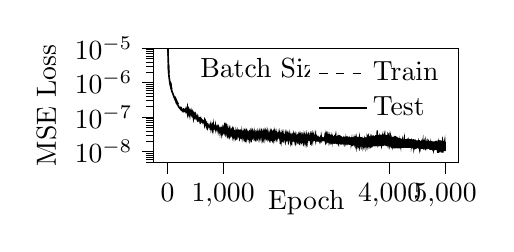
\begin{tikzpicture}

\begin{axis}[
legend cell align={left},
legend style={draw=none},
log basis y={10},
tick align=outside,
tick pos=left,
title={Batch Size 2},
title style={at={(0.4,0.85)},anchor=north},
x grid style={white!69.0196078431373!black},
xlabel={Epoch},
x label style={yshift=13pt},
xmin=-249.95, xmax=5248.95,
xtick style={color=black},
xtick = {0,1000,4000,5000},
y grid style={white!69.0196078431373!black},
ylabel={MSE Loss},
ymin=4.90143384155618e-09, ymax=1e-5,
ymode=log,
ytick style={color=black},
width=.45\textwidth,
height=.25\textwidth
]
\addplot [semithick, black, dashed]
table {%
0 0.00261398348659895
1 0.000146684363119675
2 7.82634508095725e-05
3 3.37719028447054e-05
4 2.5150746102085e-05
5 2.14879413085001e-05
6 1.73131360368757e-05
7 1.25710438198219e-05
8 8.384994563432e-06
9 6.01536302192685e-06
10 5.04094846438363e-06
11 4.50247262365266e-06
12 4.07342948584244e-06
13 3.68863333453007e-06
14 3.33568109506999e-06
15 3.02494765912797e-06
16 2.7562514826851e-06
17 2.52888349787028e-06
18 2.34137056487427e-06
19 2.18880018897138e-06
20 2.06381847633885e-06
21 1.96098151437774e-06
22 1.87465510770934e-06
23 1.80052594150659e-06
24 1.73351173886616e-06
25 1.67263015383323e-06
26 1.61614738892268e-06
27 1.56198234465066e-06
28 1.50867286552803e-06
29 1.46046563780544e-06
30 1.41356673157844e-06
31 1.37106688897681e-06
32 1.33059727563989e-06
33 1.28919083652868e-06
34 1.25175892679241e-06
35 1.21776896658865e-06
36 1.18564458267567e-06
37 1.15591732029952e-06
38 1.12700339668681e-06
39 1.10075354224648e-06
40 1.07587387876951e-06
41 1.05260377831939e-06
42 1.0313208120829e-06
43 1.01144230139827e-06
44 9.92442267119031e-07
45 9.7406527741839e-07
46 9.57213383753874e-07
47 9.40670659906218e-07
48 9.25038841827153e-07
49 9.10250043492766e-07
50 8.96198767826206e-07
51 8.83881172112133e-07
52 8.71137165300517e-07
53 8.58803400506147e-07
54 8.4801414614688e-07
55 8.36522416101104e-07
56 8.25851773152308e-07
57 8.15359453404163e-07
58 8.05294669189216e-07
59 7.95505481549164e-07
60 7.86104835461821e-07
61 7.76836224471111e-07
62 7.67232828448705e-07
63 7.40208569903089e-07
64 7.24697941538288e-07
65 7.12473284208315e-07
66 6.98334301669767e-07
67 6.8646508113801e-07
68 6.76835167410239e-07
69 6.67913647898644e-07
70 6.59476819643956e-07
71 6.51745536447201e-07
72 6.44344590145174e-07
73 6.37315424147467e-07
74 6.29807009134176e-07
75 6.23752871640626e-07
76 6.17110982172875e-07
77 6.10710473006648e-07
78 6.04971023602019e-07
79 5.99273899850594e-07
80 5.93674280890077e-07
81 5.88465108357639e-07
82 5.83262429605824e-07
83 5.78088403622168e-07
84 5.73076810137074e-07
85 5.68146300770955e-07
86 5.63457285606361e-07
87 5.59085755743816e-07
88 5.54764195544344e-07
89 5.50326957575287e-07
90 5.46110211153916e-07
91 5.41905436579171e-07
92 5.38032570275071e-07
93 5.33861362991495e-07
94 5.29962581785171e-07
95 5.25934999759059e-07
96 5.21953731732694e-07
97 5.17996030810153e-07
98 5.13999557568923e-07
99 5.10104440494707e-07
100 5.06136233847876e-07
101 5.02081006532151e-07
102 4.98216791648076e-07
103 4.94461015678738e-07
104 4.90604048617449e-07
105 4.86462815026734e-07
106 4.82587882216556e-07
107 4.78588768475063e-07
108 4.74869900535246e-07
109 4.7077929747541e-07
110 4.66663813166512e-07
111 4.62867599476446e-07
112 4.58659658813865e-07
113 4.54709814113663e-07
114 4.50870674558068e-07
115 4.46929221819659e-07
116 4.42388200826649e-07
117 4.38506839680386e-07
118 4.34678859113191e-07
119 4.3089226689208e-07
120 4.27085763439194e-07
121 4.23271578807061e-07
122 4.19777154811563e-07
123 4.15960641148239e-07
124 4.12074457444511e-07
125 4.08489014579239e-07
126 4.04658556217186e-07
127 4.00951681431394e-07
128 3.9733187562252e-07
129 3.93702260550022e-07
130 3.90062106880862e-07
131 3.86685338110482e-07
132 3.83489258807046e-07
133 3.79915736270497e-07
134 3.76464143924338e-07
135 3.73031685953151e-07
136 3.69614877314461e-07
137 3.66566005281399e-07
138 3.63254276162017e-07
139 3.59711858066269e-07
140 3.56280412384891e-07
141 3.52569088435395e-07
142 3.49126307100711e-07
143 3.45766744868303e-07
144 3.42371599904911e-07
145 3.39262808538354e-07
146 3.36348832967737e-07
147 3.33401700036262e-07
148 3.30368856395147e-07
149 3.2688863233421e-07
150 3.24198848596247e-07
151 3.21372436439926e-07
152 3.17807970312778e-07
153 3.15233077704757e-07
154 3.12444794476452e-07
155 3.10027523902079e-07
156 3.07321188873999e-07
157 3.04717508505359e-07
158 3.02148876103026e-07
159 2.99573802886144e-07
160 2.96987011524585e-07
161 2.94648659848296e-07
162 2.92419047800419e-07
163 2.90140671955541e-07
164 2.88099955823906e-07
165 2.8558504167453e-07
166 2.83444139733025e-07
167 2.8141647362645e-07
168 2.79245677041295e-07
169 2.77200937237154e-07
170 2.75588299680773e-07
171 2.73590638562027e-07
172 2.71654279449418e-07
173 2.69519297966259e-07
174 2.67458664513498e-07
175 2.65497534967629e-07
176 2.63673217523852e-07
177 2.61948017285185e-07
178 2.60005301479183e-07
179 2.58152771367648e-07
180 2.56357327418133e-07
181 2.54637377330891e-07
182 2.5292912211583e-07
183 2.51359738450141e-07
184 2.49551562201411e-07
185 2.48045789688955e-07
186 2.46444842606497e-07
187 2.4465752219438e-07
188 2.43001887576533e-07
189 2.41387644265956e-07
190 2.39743852080032e-07
191 2.38591042211134e-07
192 2.36896491812466e-07
193 2.35331076664291e-07
194 2.33869138022147e-07
195 2.32390313131603e-07
196 2.30942950676827e-07
197 2.29478455254561e-07
198 2.28119508614011e-07
199 2.26882294488195e-07
200 2.25635528665613e-07
201 2.24384542468314e-07
202 2.23268744437011e-07
203 2.21910245763457e-07
204 2.20867471478314e-07
205 2.19511795347405e-07
206 2.18217545115529e-07
207 2.17078903803181e-07
208 2.15910442586509e-07
209 2.14819290250023e-07
210 2.1386440760951e-07
211 2.12621667512458e-07
212 2.11595954674237e-07
213 2.10598725390199e-07
214 2.09534008213996e-07
215 2.08534801116933e-07
216 2.07571893242164e-07
217 2.06601709264564e-07
218 2.05631415472141e-07
219 2.04732785008765e-07
220 2.03928731128844e-07
221 2.02986788394366e-07
222 2.02125836123557e-07
223 2.01693005556169e-07
224 2.00247696379385e-07
225 1.99351367456746e-07
226 1.9847183270949e-07
227 1.97567987980651e-07
228 1.96726100124334e-07
229 1.95874223668291e-07
230 1.95032362352077e-07
231 1.9429453191222e-07
232 1.93577463155847e-07
233 1.92833159978534e-07
234 1.91930465522017e-07
235 1.91151176648585e-07
236 1.90727425620985e-07
237 1.89940357579133e-07
238 1.89282947241409e-07
239 1.88559956265433e-07
240 1.87832262899867e-07
241 1.87312221969105e-07
242 1.8638003640481e-07
243 1.85629820950606e-07
244 1.84861143206927e-07
245 1.84173773354779e-07
246 1.8346385132828e-07
247 1.82691622820474e-07
248 1.81981703223588e-07
249 1.81241538350196e-07
250 1.80819522359599e-07
251 1.80233316547929e-07
252 1.79373761339141e-07
253 1.78795408649846e-07
254 1.78261502097099e-07
255 1.77732386884122e-07
256 1.77024827346939e-07
257 1.76212229890949e-07
258 1.75559959624039e-07
259 1.75028014774092e-07
260 1.74455442444987e-07
261 1.73865569054188e-07
262 1.73293729991419e-07
263 1.72699000502652e-07
264 1.72175157529209e-07
265 1.71600795157545e-07
266 1.71060159445346e-07
267 1.70516953865052e-07
268 1.69965971575703e-07
269 1.69306111652556e-07
270 1.68603019955915e-07
271 1.68096036264442e-07
272 1.67533045300372e-07
273 1.67098511944852e-07
274 1.66452356481939e-07
275 1.6594090199118e-07
276 1.65430003029599e-07
277 1.6504094741765e-07
278 1.64535466716353e-07
279 1.64067817844948e-07
280 1.63518295869691e-07
281 1.63008348729843e-07
282 1.62516949801628e-07
283 1.62122773014195e-07
284 1.61727112577337e-07
285 1.61419068025026e-07
286 1.60981843060126e-07
287 1.60612840249152e-07
288 1.60113057938505e-07
289 1.59996616506453e-07
290 1.59500434703475e-07
291 1.59041253554371e-07
292 1.58633176553291e-07
293 1.58230017347494e-07
294 1.57726207859366e-07
295 1.57391601654178e-07
296 1.56932869004311e-07
297 1.56524124702795e-07
298 1.56090241693274e-07
299 1.55728700207858e-07
300 1.55397476291563e-07
301 1.54913462214301e-07
302 1.54460410595414e-07
303 1.54037259622264e-07
304 1.53807496733549e-07
305 1.53307295429617e-07
306 1.52889717186522e-07
307 1.52815606427659e-07
308 1.5255875534792e-07
309 1.51992299653791e-07
310 1.51631543023223e-07
311 1.51434879765988e-07
312 1.50798544854336e-07
313 1.50500502398065e-07
314 1.50309462715548e-07
315 1.5012875835807e-07
316 1.49606689905601e-07
317 1.49262755533508e-07
318 1.489406507591e-07
319 1.48563328749907e-07
320 1.48307872039899e-07
321 1.47996224146629e-07
322 1.47477975280585e-07
323 1.46864158302451e-07
324 1.46399182789247e-07
325 1.4600326030334e-07
326 1.45447961132694e-07
327 1.45286996641181e-07
328 1.45124027577159e-07
329 1.4457256800382e-07
330 1.44243595714633e-07
331 1.43893380800231e-07
332 1.43401146519118e-07
333 1.43232647254354e-07
334 1.42721284159375e-07
335 1.42463075213817e-07
336 1.42195513040511e-07
337 1.41774924736993e-07
338 1.41613115455463e-07
339 1.41290982773601e-07
340 1.40814341321294e-07
341 1.40588078612947e-07
342 1.40190531043416e-07
343 1.39982248199333e-07
344 1.39655671995254e-07
345 1.39315308924859e-07
346 1.39008234261606e-07
347 1.38621841989428e-07
348 1.38385781822015e-07
349 1.38106749037359e-07
350 1.37768745258837e-07
351 1.37302368972358e-07
352 1.37273293095319e-07
353 1.36685038603535e-07
354 1.36805641671289e-07
355 1.36218938038724e-07
356 1.36174170560555e-07
357 1.35144350333238e-07
358 1.35377791940172e-07
359 1.3519789696903e-07
360 1.34321391878522e-07
361 1.34628653254643e-07
362 1.34382502061214e-07
363 1.33540979393221e-07
364 1.33748807011447e-07
365 1.33484170640186e-07
366 1.32627974005484e-07
367 1.3297263567158e-07
368 1.32693508702708e-07
369 1.32514474537659e-07
370 1.32011076459548e-07
371 1.31861206790651e-07
372 1.31521757749109e-07
373 1.31331652518663e-07
374 1.31312317972254e-07
375 1.30603197236123e-07
376 1.30561156867826e-07
377 1.29773564399915e-07
378 1.30057639510683e-07
379 1.29861310177226e-07
380 1.29112238212326e-07
381 1.29198381696227e-07
382 1.28842748736258e-07
383 1.2872677043152e-07
384 1.2815145879741e-07
385 1.28243387647053e-07
386 1.28023895214824e-07
387 1.27487541142557e-07
388 1.27568656234978e-07
389 1.27031404781208e-07
390 1.27159839126145e-07
391 1.26598800443301e-07
392 1.26791784661684e-07
393 1.26477510927092e-07
394 1.26444590979657e-07
395 1.26158001562349e-07
396 1.25962107867528e-07
397 1.25775401044637e-07
398 1.25593913733013e-07
399 1.24813759142306e-07
400 1.25107088592591e-07
401 1.24789898830358e-07
402 1.24521163066271e-07
403 1.24255962218545e-07
404 1.24277898207348e-07
405 1.23580057124872e-07
406 1.23692217324445e-07
407 1.23466668605632e-07
408 1.23292362624872e-07
409 1.23125864866624e-07
410 1.22844255137977e-07
411 1.22260624106474e-07
412 1.22632293348746e-07
413 1.22149892797907e-07
414 1.21888570189244e-07
415 1.2183269884436e-07
416 1.21501794058565e-07
417 1.21598056354921e-07
418 1.21115364892788e-07
419 1.20845609222542e-07
420 1.20702182457633e-07
421 1.20670180585147e-07
422 1.20313101976244e-07
423 1.20242447746888e-07
424 1.19796707906294e-07
425 1.19679437805553e-07
426 1.19502443590935e-07
427 1.19306255657259e-07
428 1.19001857039169e-07
429 1.18975247541897e-07
430 1.18751168056708e-07
431 1.18668970422453e-07
432 1.18519750465174e-07
433 1.18310549850564e-07
434 1.18205436012264e-07
435 1.18052298470728e-07
436 1.17879357376394e-07
437 1.17379495784053e-07
438 1.17300958525135e-07
439 1.17437472770154e-07
440 1.17254779579357e-07
441 1.16698817170358e-07
442 1.1665886642831e-07
443 1.16422076178457e-07
444 1.16437312810413e-07
445 1.16211605543537e-07
446 1.15907504869339e-07
447 1.15631951317585e-07
448 1.15533178603799e-07
449 1.1553922251073e-07
450 1.15184505566468e-07
451 1.15018143974188e-07
452 1.15032055581388e-07
453 1.14700197587414e-07
454 1.14470164584324e-07
455 1.14392085056592e-07
456 1.14392627027948e-07
457 1.13851511679419e-07
458 1.13809522381825e-07
459 1.13363633469143e-07
460 1.13507051060058e-07
461 1.12955144015325e-07
462 1.12687809270984e-07
463 1.12958656940165e-07
464 1.12561146591084e-07
465 1.1211510408593e-07
466 1.11795333277431e-07
467 1.11874699544767e-07
468 1.11499599053211e-07
469 1.11183911756685e-07
470 1.1097315462405e-07
471 1.10746568335651e-07
472 1.10528108287378e-07
473 1.10256356484095e-07
474 1.10099632397498e-07
475 1.09766951710499e-07
476 1.09138375835371e-07
477 1.08834864133156e-07
478 1.0881889858938e-07
479 1.08393336007095e-07
480 1.08144232992657e-07
481 1.0793406884968e-07
482 1.07731355728502e-07
483 1.07404242227993e-07
484 1.07224436205255e-07
485 1.06623043470755e-07
486 1.06600979004057e-07
487 1.06223428439911e-07
488 1.06042661533579e-07
489 1.05791827745172e-07
490 1.05572618482874e-07
491 1.05332027782401e-07
492 1.05210153051427e-07
493 1.04844322206032e-07
494 1.04628191569089e-07
495 1.04377984629922e-07
496 1.04216347538877e-07
497 1.03955194479699e-07
498 1.03688604859542e-07
499 1.03510769820403e-07
500 1.03342628648528e-07
501 1.03084363703987e-07
502 1.0284133121341e-07
503 1.02668651758897e-07
504 1.02572349458985e-07
505 1.02124076692522e-07
506 1.01995372278507e-07
507 1.01731550677941e-07
508 1.01490412855565e-07
509 1.01381675744916e-07
510 1.01240593376462e-07
511 1.00909068223354e-07
512 1.00669337769643e-07
513 1.00404250107822e-07
514 1.00423404139294e-07
515 1.00214220461581e-07
516 9.99527497607122e-08
517 9.97062718719466e-08
518 9.94624701242675e-08
519 9.93852768302883e-08
520 9.90874772937023e-08
521 9.88455424544288e-08
522 9.86786483039293e-08
523 9.85174300247582e-08
524 9.83541504726571e-08
525 9.82658134411896e-08
526 9.78364765480411e-08
527 9.77660970995498e-08
528 9.7614606940466e-08
529 9.7288654843819e-08
530 9.69792118370449e-08
531 9.69268959594149e-08
532 9.67892044398955e-08
533 9.64910404850361e-08
534 9.62170009874974e-08
535 9.62202412035929e-08
536 9.58558749346583e-08
537 9.56776447187391e-08
538 9.5498134587757e-08
539 9.53894120798715e-08
540 9.50934551380289e-08
541 9.48801197169224e-08
542 9.46125329708281e-08
543 9.44436887060363e-08
544 9.4335708752169e-08
545 9.40767704953327e-08
546 9.38061104351906e-08
547 9.36843962597855e-08
548 9.34865146009489e-08
549 9.32645453668446e-08
550 9.30323500869523e-08
551 9.2910364995813e-08
552 9.24915208440069e-08
553 9.26237489684567e-08
554 9.20383658806756e-08
555 9.20737594465315e-08
556 9.1773045729715e-08
557 9.15990957992552e-08
558 9.16372675546784e-08
559 9.13390870608266e-08
560 9.12179028298432e-08
561 9.10503901381254e-08
562 9.07964728142918e-08
563 9.05843692435848e-08
564 9.03890795960205e-08
565 9.00719094163449e-08
566 8.99008989017069e-08
567 8.98419131223349e-08
568 8.94903660499935e-08
569 8.92771059846087e-08
570 8.92133772965043e-08
571 8.92505096738994e-08
572 8.88596866948088e-08
573 8.88809712964456e-08
574 8.85358828333072e-08
575 8.83346679561026e-08
576 8.84105503005106e-08
577 8.8131889763865e-08
578 8.80912545679902e-08
579 8.76220811723005e-08
580 8.76374261120638e-08
581 8.73306817090747e-08
582 8.69455808030217e-08
583 8.70990354120416e-08
584 8.65921273616177e-08
585 8.64360111918483e-08
586 8.64471381185616e-08
587 8.61044444553372e-08
588 8.59900289835735e-08
589 8.59733905260729e-08
590 8.56495371353017e-08
591 8.5448452592729e-08
592 8.52556495878343e-08
593 8.50720472700406e-08
594 8.48990268551564e-08
595 8.46750809213592e-08
596 8.45080046549818e-08
597 8.42445121276292e-08
598 8.40143372828894e-08
599 8.37218631160042e-08
600 8.35349402392716e-08
601 8.31654908488577e-08
602 8.30242949245719e-08
603 8.2982439593593e-08
604 8.2921621885168e-08
605 8.26500533532837e-08
606 8.25823081787025e-08
607 8.2389301115926e-08
608 8.22421491531999e-08
609 8.19840703343289e-08
610 8.1801761944611e-08
611 8.18592255097395e-08
612 8.16676565214003e-08
613 8.16171640491969e-08
614 8.13247282057672e-08
615 8.10373738009407e-08
616 8.08642084723088e-08
617 8.06555648807938e-08
618 8.039214622102e-08
619 8.02460349925704e-08
620 8.00810798282647e-08
621 7.99409526959227e-08
622 7.97110490066144e-08
623 7.94116076875406e-08
624 7.92543457824868e-08
625 7.90482818721072e-08
626 7.87830216444352e-08
627 7.86491988641336e-08
628 7.84446622161816e-08
629 7.827243654146e-08
630 7.81483883874889e-08
631 7.79432979882699e-08
632 7.77564276402964e-08
633 7.75270853509147e-08
634 7.74125279346949e-08
635 7.70996542881486e-08
636 7.70233436728773e-08
637 7.66381009270622e-08
638 7.64740521639329e-08
639 7.66816242462332e-08
640 7.64246416755654e-08
641 7.61894967465926e-08
642 7.59976832137577e-08
643 7.56666841013054e-08
644 7.54723867576468e-08
645 7.54306852314146e-08
646 7.53268538478125e-08
647 7.51730338366396e-08
648 7.47495809915177e-08
649 7.48541830168925e-08
650 7.43791588843079e-08
651 7.42978026984087e-08
652 7.42460074155682e-08
653 7.40438198457705e-08
654 7.3634554738522e-08
655 7.37113431152903e-08
656 7.34467651670734e-08
657 7.33724932918678e-08
658 7.31816905603644e-08
659 7.31439444945359e-08
660 7.28667297711372e-08
661 7.26887656533615e-08
662 7.25385389976907e-08
663 7.24498825926956e-08
664 7.22832119443018e-08
665 7.21822083353807e-08
666 7.19495448092688e-08
667 7.18707898982318e-08
668 7.16480042597389e-08
669 7.14073806823423e-08
670 7.13205865152666e-08
671 7.10196900129967e-08
672 7.09722795270151e-08
673 7.07187652627672e-08
674 7.06024032132158e-08
675 7.05165593821722e-08
676 7.03380461603009e-08
677 7.03425385415457e-08
678 7.00737257445239e-08
679 6.99320477606236e-08
680 6.97025158427067e-08
681 6.95539946653501e-08
682 6.93178849876519e-08
683 6.94211070342288e-08
684 6.90671745279259e-08
685 6.8847339870004e-08
686 6.89086112218851e-08
687 6.87327516597502e-08
688 6.84967959185823e-08
689 6.84914813144921e-08
690 6.84173265950161e-08
691 6.81482263986677e-08
692 6.79657498626751e-08
693 6.76911481836129e-08
694 6.78754415739391e-08
695 6.76873341790563e-08
696 6.7420077696112e-08
697 6.73318192355721e-08
698 6.71849346519648e-08
699 6.70631731659599e-08
700 6.6936109860527e-08
701 6.67347293343834e-08
702 6.66230708357141e-08
703 6.67056503975694e-08
704 6.66208884274599e-08
705 6.6402336841076e-08
706 6.637572022683e-08
707 6.60298795550629e-08
708 6.58703416722695e-08
709 6.59932807797192e-08
710 6.57574264092409e-08
711 6.5755870203299e-08
712 6.55362282209193e-08
713 6.54728074114264e-08
714 6.5351697348004e-08
715 6.53087951680842e-08
716 6.51708659051842e-08
717 6.50125667877033e-08
718 6.49798564733572e-08
719 6.47724273014072e-08
720 6.47707329970437e-08
721 6.45535312721046e-08
722 6.44558372296933e-08
723 6.43093136186712e-08
724 6.406546154758e-08
725 6.40719362525743e-08
726 6.45583160179264e-08
727 6.38616268305858e-08
728 6.39997100977396e-08
729 6.38944717001877e-08
730 6.37970664736365e-08
731 6.36738414186988e-08
732 6.35405101436781e-08
733 6.3468621691154e-08
734 6.31237134999241e-08
735 6.32146194542438e-08
736 6.31069264531714e-08
737 6.30518270504643e-08
738 6.29606186937082e-08
739 6.26848402600633e-08
740 6.28600875853813e-08
741 6.26476349310234e-08
742 6.24892591627457e-08
743 6.24455489549591e-08
744 6.23294498194316e-08
745 6.2253770162779e-08
746 6.21718271596183e-08
747 6.20670583866279e-08
748 6.18798210956228e-08
749 6.188538615437e-08
750 6.18037680910621e-08
751 6.16810066836893e-08
752 6.15384937397989e-08
753 6.14532277937174e-08
754 6.1445070853372e-08
755 6.13365998902715e-08
756 6.12798440569051e-08
757 6.13104954930721e-08
758 6.12681508648238e-08
759 6.10669092498961e-08
760 6.10586326349472e-08
761 6.09786342657959e-08
762 6.08765920058207e-08
763 6.07757833117617e-08
764 6.07843563827926e-08
765 6.05380540213973e-08
766 6.04225618350274e-08
767 6.03992417815835e-08
768 6.03464287243227e-08
769 6.01462231776262e-08
770 6.00604040950081e-08
771 6.00231084527669e-08
772 5.99093010943408e-08
773 5.98377934263317e-08
774 5.96081898500689e-08
775 5.95742457141224e-08
776 5.96780586127332e-08
777 5.93245081615956e-08
778 5.91501711765252e-08
779 5.92791223117395e-08
780 5.91412333191821e-08
781 5.90747720404794e-08
782 5.89476858179339e-08
783 5.88208731741036e-08
784 5.88255402458326e-08
785 5.8786889870488e-08
786 5.86065183543205e-08
787 5.86318991023793e-08
788 5.8584062483602e-08
789 5.84684124078638e-08
790 5.85145645294327e-08
791 5.82407579362565e-08
792 5.82223076095456e-08
793 5.79912457159271e-08
794 5.8108856008543e-08
795 5.79709602686052e-08
796 5.78531142740868e-08
797 5.78370420644125e-08
798 5.76913316553407e-08
799 5.76839951780261e-08
800 5.75831435745133e-08
801 5.75909274685982e-08
802 5.74083612785437e-08
803 5.74391697699683e-08
804 5.72027329296398e-08
805 5.73407223503075e-08
806 5.72023227312091e-08
807 5.70735137997991e-08
808 5.70729130350278e-08
809 5.69626252675537e-08
810 5.6882644279832e-08
811 5.68058462963039e-08
812 5.66683241300936e-08
813 5.66744659303842e-08
814 5.65901798542656e-08
815 5.6436309426422e-08
816 5.65831056307253e-08
817 5.63878848396371e-08
818 5.62771926944095e-08
819 5.62657206842898e-08
820 5.62157826032861e-08
821 5.61009023639647e-08
822 5.60516779550824e-08
823 5.59690822986569e-08
824 5.61079724488156e-08
825 5.58611277436949e-08
826 5.57958161638838e-08
827 5.57157521758889e-08
828 5.56878466763111e-08
829 5.57414290146552e-08
830 5.54114399603511e-08
831 5.54050776053749e-08
832 5.54322031087739e-08
833 5.54243826426104e-08
834 5.53643694637396e-08
835 5.51954801198962e-08
836 5.53016565781883e-08
837 5.52197657462949e-08
838 5.50475004045259e-08
839 5.50929451459403e-08
840 5.49398851192873e-08
841 5.50032194527317e-08
842 5.49059920349482e-08
843 5.48543149434533e-08
844 5.47220845609209e-08
845 5.45919308593268e-08
846 5.46621458888952e-08
847 5.45036415513511e-08
848 5.44871118437484e-08
849 5.44909918462899e-08
850 5.44362895656958e-08
851 5.42284673225035e-08
852 5.43319143780918e-08
853 5.42738582536284e-08
854 5.39490024304978e-08
855 5.41623808413272e-08
856 5.38711755492249e-08
857 5.38292376828231e-08
858 5.38144721166089e-08
859 5.40801493253973e-08
860 5.35556771573686e-08
861 5.34009007191472e-08
862 5.36913170899878e-08
863 5.35750088621612e-08
864 5.34702983183699e-08
865 5.31324628701979e-08
866 5.32663798854527e-08
867 5.34713005498899e-08
868 5.3268240315818e-08
869 5.3106281430626e-08
870 5.30999553991496e-08
871 5.30073745623749e-08
872 5.3024831385029e-08
873 5.29475644116539e-08
874 5.29035295295799e-08
875 5.27633898719237e-08
876 5.27644872644339e-08
877 5.26363374481198e-08
878 5.21344579949012e-08
879 5.26222953115552e-08
880 5.25046283263997e-08
881 5.25887310142137e-08
882 5.23786171260365e-08
883 5.22556745392588e-08
884 5.22890715103364e-08
885 5.22051752521735e-08
886 5.22562960395545e-08
887 5.21403642420593e-08
888 5.21259177299616e-08
889 5.23303570957312e-08
890 5.21940686630806e-08
891 5.20369648042696e-08
892 5.18643744533698e-08
893 5.1959078596342e-08
894 5.1800517703815e-08
895 5.17839124822839e-08
896 5.1749980221838e-08
897 5.20235737372365e-08
898 5.14930678036096e-08
899 5.13947631269884e-08
900 5.14576784906851e-08
901 5.15045462358144e-08
902 5.14380473438658e-08
903 5.14084751558341e-08
904 5.13051172055246e-08
905 5.13162940889433e-08
906 5.12426185311776e-08
907 5.11894807858626e-08
908 5.12040236309019e-08
909 5.11771593126875e-08
910 5.1391161834613e-08
911 5.09132827229974e-08
912 5.07956156252654e-08
913 5.07086769411247e-08
914 5.07240060290126e-08
915 5.05156226283665e-08
916 5.09034994145008e-08
917 5.10812179872477e-08
918 5.09299017443787e-08
919 5.06071179470213e-08
920 5.06153786566932e-08
921 5.08228125277732e-08
922 5.07701664046456e-08
923 5.04631669587807e-08
924 5.04625080791632e-08
925 5.03999359618978e-08
926 5.03120141140956e-08
927 5.02950299255955e-08
928 5.02036412520779e-08
929 5.05533185670704e-08
930 5.03805240215094e-08
931 5.03134604930011e-08
932 5.03399029133655e-08
933 5.02495765224431e-08
934 5.02485439819456e-08
935 5.01097002670869e-08
936 4.98450323295208e-08
937 5.00081839931443e-08
938 5.02201354417586e-08
939 5.00173292057315e-08
940 4.99454150872936e-08
941 4.98917330522541e-08
942 4.97869760859304e-08
943 4.96477238839388e-08
944 4.96061485512067e-08
945 4.96272340385628e-08
946 4.96270244700892e-08
947 4.96611786039436e-08
948 4.93043708666985e-08
949 4.93675331766363e-08
950 4.94701070694603e-08
951 4.95901512781449e-08
952 4.95660200040549e-08
953 4.93224323655506e-08
954 4.91889253581013e-08
955 4.92657079411152e-08
956 4.93090457755474e-08
957 4.90304114769136e-08
958 4.86113878614414e-08
959 4.87386970814407e-08
960 4.86080396257527e-08
961 4.91473815086851e-08
962 4.82496446461145e-08
963 4.8349681513904e-08
964 4.83994517888053e-08
965 4.84674849848266e-08
966 4.89019669674406e-08
967 4.87339815461452e-08
968 4.8887384868801e-08
969 4.86750621041532e-08
970 4.87458362598003e-08
971 4.87206623641101e-08
972 4.85998083747385e-08
973 4.86616961933861e-08
974 4.85624361134529e-08
975 4.85805682470253e-08
976 4.85125720613433e-08
977 4.82887160206391e-08
978 4.84719224294605e-08
979 4.83484899962972e-08
980 4.82735046126725e-08
981 4.84206677583976e-08
982 4.82095535099814e-08
983 4.81738937898046e-08
984 4.81529513432499e-08
985 4.80463511752238e-08
986 4.8008118166909e-08
987 4.78388747605085e-08
988 4.79545476203547e-08
989 4.77904276480756e-08
990 4.76947455610444e-08
991 4.7953770904885e-08
992 4.75322841403392e-08
993 4.7785734386907e-08
994 4.75348239130091e-08
995 4.7667171884147e-08
996 4.74739370615596e-08
997 4.75618149212709e-08
998 4.75811124144854e-08
999 4.74248252290144e-08
1000 4.76309443844802e-08
1001 4.72376396284391e-08
1002 4.71671802128038e-08
1003 4.74440110288521e-08
1004 4.69942068811458e-08
1005 4.71157604259309e-08
1006 4.69819341240574e-08
1007 4.69522687752133e-08
1008 4.68813971180038e-08
1009 4.66572676727783e-08
1010 4.68712826183215e-08
1011 4.65230975445485e-08
1012 4.6986280031025e-08
1013 4.65285257113535e-08
1014 4.65172853401641e-08
1015 4.69000739997116e-08
1016 4.59802069521786e-08
1017 4.61438803179282e-08
1018 4.61487103370906e-08
1019 4.60385496252047e-08
1020 4.60279651077755e-08
1021 4.5991702721071e-08
1022 4.6049907213741e-08
1023 4.58232247232404e-08
1024 4.575472711843e-08
1025 4.57867423995784e-08
1026 4.57194202890809e-08
1027 4.5735625373744e-08
1028 4.56614160241897e-08
1029 4.57159697072051e-08
1030 4.55817242379086e-08
1031 4.55687318516862e-08
1032 4.55431716767651e-08
1033 4.54868766998073e-08
1034 4.54809728112071e-08
1035 4.53985480052266e-08
1036 4.5422408025686e-08
1037 4.52892244754421e-08
1038 4.52831030046119e-08
1039 4.53999871000699e-08
1040 4.54181504337958e-08
1041 4.52862972734613e-08
1042 4.51580050345179e-08
1043 4.51480138310423e-08
1044 4.51643003261393e-08
1045 4.51240597721392e-08
1046 4.49955824772252e-08
1047 4.50499606158838e-08
1048 4.50189186058103e-08
1049 4.50657565729817e-08
1050 4.4959013388024e-08
1051 4.48627814274016e-08
1052 4.48606086906889e-08
1053 4.4802549736378e-08
1054 4.48229560718882e-08
1055 4.48897614062638e-08
1056 4.47645272669828e-08
1057 4.46646057877254e-08
1058 4.47493429872603e-08
1059 4.46290876262023e-08
1060 4.47393384138683e-08
1061 4.44872028639853e-08
1062 4.46542057774835e-08
1063 4.44682002784802e-08
1064 4.45064564659758e-08
1065 4.45753047110253e-08
1066 4.4414909836088e-08
1067 4.44585654978957e-08
1068 4.43124520668192e-08
1069 4.43833488869561e-08
1070 4.4300507340167e-08
1071 4.42940364882016e-08
1072 4.42912890031288e-08
1073 4.43040135522099e-08
1074 4.42048048830967e-08
1075 4.416254044598e-08
1076 4.41335653407759e-08
1077 4.40365813249022e-08
1078 4.41081502742802e-08
1079 4.40969820470483e-08
1080 4.3948786994652e-08
1081 4.41720446373584e-08
1082 4.39464986777271e-08
1083 4.40942140758627e-08
1084 4.37837767735538e-08
1085 4.39278263835718e-08
1086 4.37930967392974e-08
1087 4.37182112345003e-08
1088 4.37573598288665e-08
1089 4.37867421974048e-08
1090 4.36447713969557e-08
1091 4.38515382742977e-08
1092 4.37362916652084e-08
1093 4.36174015362445e-08
1094 4.3778218633217e-08
1095 4.35680120209891e-08
1096 4.35805192225414e-08
1097 4.36738350335086e-08
1098 4.36676859579821e-08
1099 4.35005779383379e-08
1100 4.35071349083049e-08
1101 4.35172271734396e-08
1102 4.34009853089168e-08
1103 4.33678863978049e-08
1104 4.33504221901138e-08
1105 4.32441569210851e-08
1106 4.3280685350644e-08
1107 4.34523939446541e-08
1108 4.32948200780325e-08
1109 4.31160244203088e-08
1110 4.31606878995017e-08
1111 4.31132841002824e-08
1112 4.31126667642112e-08
1113 4.30161841746823e-08
1114 4.31351706885463e-08
1115 4.30137107217399e-08
1116 4.30419452301378e-08
1117 4.28521687167449e-08
1118 4.29494802055563e-08
1119 4.2983084970083e-08
1120 4.28279311986968e-08
1121 4.29285861436868e-08
1122 4.28456561525348e-08
1123 4.29562623107116e-08
1124 4.28213921451759e-08
1125 4.27720357785155e-08
1126 4.27197061031448e-08
1127 4.27676665794574e-08
1128 4.27508851308933e-08
1129 4.2682300908925e-08
1130 4.26003897978089e-08
1131 4.24758110147416e-08
1132 4.25463953803162e-08
1133 4.25152052525024e-08
1134 4.25598208884104e-08
1135 4.239308792503e-08
1136 4.2449155177704e-08
1137 4.24381763784454e-08
1138 4.24335556179489e-08
1139 4.23089017043132e-08
1140 4.23211221574071e-08
1141 4.22933782630586e-08
1142 4.23067300873714e-08
1143 4.23677056163863e-08
1144 4.23486314717891e-08
1145 4.19986635529779e-08
1146 4.20469467001805e-08
1147 4.22094996923028e-08
1148 4.20193057089624e-08
1149 4.21166019328179e-08
1150 4.21501204259656e-08
1151 4.19883999723814e-08
1152 4.20073089106854e-08
1153 4.18943582077835e-08
1154 4.19936113004726e-08
1155 4.20366788216886e-08
1156 4.20818990342631e-08
1157 4.18583599697264e-08
1158 4.17444217319929e-08
1159 4.17618667362674e-08
1160 4.17829855202667e-08
1161 4.17799846383904e-08
1162 4.16705735562517e-08
1163 4.18948547789011e-08
1164 4.16620335019213e-08
1165 4.17125577941713e-08
1166 4.15728996195353e-08
1167 4.16248975123046e-08
1168 4.17766256601282e-08
1169 4.14573240685168e-08
1170 4.15731547034337e-08
1171 4.14832258551212e-08
1172 4.14894388031661e-08
1173 4.17455580651316e-08
1174 4.15013680700738e-08
1175 4.15968621256257e-08
1176 4.13717257054524e-08
1177 4.15543938007135e-08
1178 4.12514978142542e-08
1179 4.14077720277683e-08
1180 4.15308862883323e-08
1181 4.13152643243264e-08
1182 4.13804941682416e-08
1183 4.13969383722401e-08
1184 4.13074685233217e-08
1185 4.14006716444315e-08
1186 4.12031826499959e-08
1187 4.13484403469777e-08
1188 4.11279918449137e-08
1189 4.1116992403778e-08
1190 4.10200866945987e-08
1191 4.10916682780371e-08
1192 4.10232857664949e-08
1193 4.11754650986307e-08
1194 4.08613160786109e-08
1195 4.10294067033634e-08
1196 4.11262635822141e-08
1197 4.09699648660222e-08
1198 4.09178326050697e-08
1199 4.08179365538608e-08
1200 4.08433911486261e-08
1201 4.07925646619955e-08
1202 4.0843865591389e-08
1203 4.08273227012201e-08
1204 4.08248592192462e-08
1205 4.09464814088434e-08
1206 4.07076831734909e-08
1207 4.06216350464228e-08
1208 4.05717194499888e-08
1209 4.07536141571185e-08
1210 4.06037834261297e-08
1211 4.05800763356723e-08
1212 4.05475472338157e-08
1213 4.05940800142779e-08
1214 4.07310513145798e-08
1215 4.0481364380951e-08
1216 4.05854570876274e-08
1217 4.0419865971697e-08
1218 4.04724098932996e-08
1219 4.03760262344677e-08
1220 4.05545208236879e-08
1221 4.04062817561668e-08
1222 4.04085032262302e-08
1223 4.0206302078627e-08
1224 4.02853182185359e-08
1225 4.02691618917039e-08
1226 4.02556384009323e-08
1227 3.99654077228306e-08
1228 4.0084840536081e-08
1229 3.99519415278937e-08
1230 3.99425685834176e-08
1231 3.99511088683413e-08
1232 3.99962168105006e-08
1233 3.98757909992886e-08
1234 3.99903259502565e-08
1235 3.97727424241157e-08
1236 3.97362323014128e-08
1237 3.98615986861861e-08
1238 3.97920895919279e-08
1239 3.96503417985916e-08
1240 3.98500998187723e-08
1241 3.94888271154081e-08
1242 3.97363479529567e-08
1243 3.9670114947099e-08
1244 3.95152142287913e-08
1245 3.94588912658311e-08
1246 3.96170589693212e-08
1247 3.95713690846677e-08
1248 3.9653338033907e-08
1249 3.96299430795444e-08
1250 3.93851973877202e-08
1251 3.95682592178592e-08
1252 3.94245985052555e-08
1253 3.94186836629173e-08
1254 3.93995191990681e-08
1255 3.94417245035417e-08
1256 3.93175576240967e-08
1257 3.93010308639696e-08
1258 3.94500662774244e-08
1259 3.92660184653781e-08
1260 3.91611785369173e-08
1261 3.93277218297405e-08
1262 3.90468253679832e-08
1263 3.92391634491673e-08
1264 3.90210088450083e-08
1265 3.90619693654837e-08
1266 3.91635332250839e-08
1267 3.91998140386596e-08
1268 3.88992044481062e-08
1269 3.92167338549299e-08
1270 3.88048741853941e-08
1271 3.90122393857384e-08
1272 3.90509703188657e-08
1273 3.89146043306421e-08
1274 3.89563392785841e-08
1275 3.89260859701701e-08
1276 3.90563198613969e-08
1277 3.903581282938e-08
1278 3.87682184300187e-08
1279 3.90418795276903e-08
1280 3.88307571365099e-08
1281 3.88432197571675e-08
1282 3.88089232857825e-08
1283 3.88497545305011e-08
1284 3.8808237176613e-08
1285 3.86636885413849e-08
1286 3.8951220149408e-08
1287 3.87320291024285e-08
1288 3.86920816649039e-08
1289 3.8919329096998e-08
1290 3.86722198195133e-08
1291 3.86278853801714e-08
1292 3.88914554788622e-08
1293 3.8599475284451e-08
1294 3.8693181822369e-08
1295 3.85323008162963e-08
1296 3.85450245753982e-08
1297 3.8618123346601e-08
1298 3.86272235451401e-08
1299 3.85501028578594e-08
1300 3.85360730471018e-08
1301 3.84817750264665e-08
1302 3.83798020365811e-08
1303 3.84028968161143e-08
1304 3.83411669929168e-08
1305 3.86072583850039e-08
1306 3.83613074982914e-08
1307 3.8552181814977e-08
1308 3.82130065704755e-08
1309 3.80664171260592e-08
1310 3.84765729979919e-08
1311 3.81774920919509e-08
1312 3.82775483957487e-08
1313 3.83419538739216e-08
1314 3.82416022891574e-08
1315 3.81589909581037e-08
1316 3.84554827882466e-08
1317 3.81900211631758e-08
1318 3.80497460764073e-08
1319 3.80913908638036e-08
1320 3.79748055899243e-08
1321 3.82118173543611e-08
1322 3.8044942906712e-08
1323 3.7897786287433e-08
1324 3.80364340222261e-08
1325 3.80164513292258e-08
1326 3.80070932131105e-08
1327 3.77907139890721e-08
1328 3.79741725815008e-08
1329 3.7962045192963e-08
1330 3.78899051253767e-08
1331 3.78060559529936e-08
1332 3.78670913306345e-08
1333 3.78315917831662e-08
1334 3.80222686703902e-08
1335 3.77478427376343e-08
1336 3.76959864369364e-08
1337 3.76758144395861e-08
1338 3.78092513653727e-08
1339 3.77412872711314e-08
1340 3.76240642890879e-08
1341 3.77037665962865e-08
1342 3.75619689473861e-08
1343 3.77010441950931e-08
1344 3.77110146798088e-08
1345 3.75804105830491e-08
1346 3.76246193385943e-08
1347 3.75692676248818e-08
1348 3.74983338812807e-08
1349 3.74260324288445e-08
1350 3.73596034612955e-08
1351 3.74343606266425e-08
1352 3.74937736646319e-08
1353 3.75229895516749e-08
1354 3.71330517868751e-08
1355 3.74137304480215e-08
1356 3.7181566376332e-08
1357 3.72471152274567e-08
1358 3.74778136069676e-08
1359 3.72647145150395e-08
1360 3.72154928966473e-08
1361 3.7239597339922e-08
1362 3.72700734292408e-08
1363 3.74581570247168e-08
1364 3.7001714643492e-08
1365 3.71595026116833e-08
1366 3.72408672513203e-08
1367 3.7080263740441e-08
1368 3.72318790692883e-08
1369 3.70415177685657e-08
1370 3.72782474327149e-08
1371 3.70204627198611e-08
1372 3.70034276288567e-08
1373 3.71566659543299e-08
1374 3.69266780143596e-08
1375 3.71390608163713e-08
1376 3.69570218351489e-08
1377 3.6941323282691e-08
1378 3.6822000582748e-08
1379 3.6959429911998e-08
1380 3.68920858652144e-08
1381 3.701040906956e-08
1382 3.681259792776e-08
1383 3.66875012499102e-08
1384 3.6890900990294e-08
1385 3.68982291191755e-08
1386 3.69947587329777e-08
1387 3.70211979827673e-08
1388 3.68647417595125e-08
1389 3.6786965299962e-08
1390 3.69163455046229e-08
1391 3.6661925532866e-08
1392 3.68543216258121e-08
1393 3.68127328680412e-08
1394 3.68141683004253e-08
1395 3.68085077421254e-08
1396 3.67071528235008e-08
1397 3.68935591985031e-08
1398 3.66122590514939e-08
1399 3.66694211784147e-08
1400 3.65310263724661e-08
1401 3.66279319389262e-08
1402 3.64981576203016e-08
1403 3.64699415433267e-08
1404 3.67245235168845e-08
1405 3.65029932370975e-08
1406 3.66564263549751e-08
1407 3.66455188268722e-08
1408 3.64214779541294e-08
1409 3.65147219616446e-08
1410 3.67536794762535e-08
1411 3.66980817745333e-08
1412 3.63030791232788e-08
1413 3.66292846185612e-08
1414 3.64065608632891e-08
1415 3.63810815168786e-08
1416 3.65551502848893e-08
1417 3.63827365366665e-08
1418 3.68315672601427e-08
1419 3.6253791672769e-08
1420 3.65551811753462e-08
1421 3.63489426132846e-08
1422 3.64301096009711e-08
1423 3.63845785113504e-08
1424 3.63241670645609e-08
1425 3.62743841785806e-08
1426 3.64269679675733e-08
1427 3.62643482531011e-08
1428 3.64093605202953e-08
1429 3.65368469820715e-08
1430 3.64458330048834e-08
1431 3.61357457412947e-08
1432 3.62946508546957e-08
1433 3.61692249251089e-08
1434 3.63927227604033e-08
1435 3.62667733102562e-08
1436 3.6191466375235e-08
1437 3.60597453187284e-08
1438 3.61780122727362e-08
1439 3.63371264393564e-08
1440 3.60288973001444e-08
1441 3.61311922566498e-08
1442 3.6101228826857e-08
1443 3.61737874227663e-08
1444 3.60708859069026e-08
1445 3.60423173657032e-08
1446 3.61806412192967e-08
1447 3.61474959655883e-08
1448 3.61653036710097e-08
1449 3.61737482946212e-08
1450 3.60483866692074e-08
1451 3.60628494541215e-08
1452 3.59418912091458e-08
1453 3.59477794594221e-08
1454 3.60916861414928e-08
1455 3.61096439289721e-08
1456 3.60066770979661e-08
1457 3.60769590888044e-08
1458 3.60448918488854e-08
1459 3.59734010469959e-08
1460 3.5930709048837e-08
1461 3.59758459184678e-08
1462 3.58558317283264e-08
1463 3.60298738923404e-08
1464 3.59392365429922e-08
1465 3.59062993798842e-08
1466 3.60486273298655e-08
1467 3.56902185318364e-08
1468 3.57968897950478e-08
1469 3.59835234380324e-08
1470 3.56674581156735e-08
1471 3.59051779348363e-08
1472 3.57930280444063e-08
1473 3.61311931985631e-08
1474 3.55918575497549e-08
1475 3.56933443580454e-08
1476 3.56426915007479e-08
1477 3.5738645992045e-08
1478 3.57809168338719e-08
1479 3.57045625825059e-08
1480 3.57558388912049e-08
1481 3.56408534146202e-08
1482 3.59447247259559e-08
1483 3.5626910365294e-08
1484 3.57225171889186e-08
1485 3.55112521048251e-08
1486 3.57546030416156e-08
1487 3.56030605532798e-08
1488 3.55800063335243e-08
1489 3.57159678091579e-08
1490 3.5622840438454e-08
1491 3.56112106800199e-08
1492 3.55408875938323e-08
1493 3.55446255211334e-08
1494 3.56145687260834e-08
1495 3.54259949193469e-08
1496 3.54903710649279e-08
1497 3.53642074025218e-08
1498 3.54873146918844e-08
1499 3.54727140838285e-08
1500 3.55334545208419e-08
1501 3.5409026780342e-08
1502 3.54803372437096e-08
1503 3.55096652833176e-08
1504 3.54438842816163e-08
1505 3.54438994277229e-08
1506 3.52586356386353e-08
1507 3.54853364768481e-08
1508 3.52613148048575e-08
1509 3.56022012296675e-08
1510 3.509981280575e-08
1511 3.56337536586149e-08
1512 3.52175760410245e-08
1513 3.53154326817595e-08
1514 3.534399718369e-08
1515 3.51297950942908e-08
1516 3.53575105652149e-08
1517 3.51708020545627e-08
1518 3.53134347643169e-08
1519 3.52938552420912e-08
1520 3.53772712797795e-08
1521 3.54995465590147e-08
1522 3.50098286754363e-08
1523 3.51518915935878e-08
1524 3.50881709478834e-08
1525 3.50589046707039e-08
1526 3.50215923819452e-08
1527 3.53548170237139e-08
1528 3.5026552623274e-08
1529 3.52368347221188e-08
1530 3.50323764222171e-08
1531 3.51654090468001e-08
1532 3.51068960543488e-08
1533 3.51634139128532e-08
1534 3.51571836484377e-08
1535 3.49424351043237e-08
1536 3.50187879449848e-08
1537 3.53500963033437e-08
1538 3.50289750721822e-08
1539 3.48855184874042e-08
1540 3.50088064540177e-08
1541 3.49903093593285e-08
1542 3.50582522964382e-08
1543 3.50921210990895e-08
1544 3.49305118901855e-08
1545 3.48348799145137e-08
1546 3.50040681207364e-08
1547 3.50324450644757e-08
1548 3.47821500198964e-08
1549 3.48002036693606e-08
1550 3.50278476385357e-08
1551 3.48182352611914e-08
1552 3.4843449333799e-08
1553 3.47927909744028e-08
1554 3.46968657146118e-08
1555 3.48270575143417e-08
1556 3.48542658725748e-08
1557 3.47570996516722e-08
1558 3.47461852138742e-08
1559 3.48612541893889e-08
1560 3.47328968683946e-08
1561 3.4757167578614e-08
1562 3.46516574474265e-08
1563 3.49862555948932e-08
1564 3.46321199928834e-08
1565 3.4780982513416e-08
1566 3.46651921784291e-08
1567 3.45752515271136e-08
1568 3.47753969680009e-08
1569 3.48198636946351e-08
1570 3.47757455861908e-08
1571 3.4507271549189e-08
1572 3.47078772566789e-08
1573 3.49576113828354e-08
1574 3.47395628798042e-08
1575 3.45694570675903e-08
1576 3.47136032560202e-08
1577 3.44184528642821e-08
1578 3.45566974758738e-08
1579 3.45180234527787e-08
1580 3.4580202604495e-08
1581 3.45497845699594e-08
1582 3.42231714617336e-08
1583 3.46553255673454e-08
1584 3.43230252612958e-08
1585 3.44667043732372e-08
1586 3.42018570680391e-08
1587 3.42796177371651e-08
1588 3.45346177799133e-08
1589 3.42886514995699e-08
1590 3.41987356230478e-08
1591 3.42419555141582e-08
1592 3.42777873509892e-08
1593 3.43240454155902e-08
1594 3.44707572889069e-08
1595 3.41868560851388e-08
1596 3.42473797330656e-08
1597 3.41525397445919e-08
1598 3.42604636796029e-08
1599 3.42073004447885e-08
1600 3.42863649285263e-08
1601 3.42130756987857e-08
1602 3.4182281366868e-08
1603 3.41949527709051e-08
1604 3.42302469623634e-08
1605 3.43229221849706e-08
1606 3.40175767419293e-08
1607 3.41228139911776e-08
1608 3.39518507423975e-08
1609 3.41163186207138e-08
1610 3.41803030444177e-08
1611 3.39146702968973e-08
1612 3.39262604691637e-08
1613 3.41989028934675e-08
1614 3.40345293181055e-08
1615 3.3939421488216e-08
1616 3.42013139937869e-08
1617 3.40021184344064e-08
1618 3.40370750067098e-08
1619 3.39722234156126e-08
1620 3.39850721161605e-08
1621 3.39282047469025e-08
1622 3.38887960671941e-08
1623 3.38494148963142e-08
1624 3.39835219518303e-08
1625 3.40568993758006e-08
1626 3.37798887363183e-08
1627 3.40222135623014e-08
1628 3.40237355868633e-08
1629 3.3838818874754e-08
1630 3.40310748536687e-08
1631 3.38542083794802e-08
1632 3.38119319162056e-08
1633 3.37274185027159e-08
1634 3.38834484395756e-08
1635 3.37319519347901e-08
1636 3.38475110375214e-08
1637 3.3742468025566e-08
1638 3.38427758715953e-08
1639 3.36246807055574e-08
1640 3.36959911075851e-08
1641 3.37534677092854e-08
1642 3.37967688742169e-08
1643 3.36699845108202e-08
1644 3.37426600273694e-08
1645 3.37344562306718e-08
1646 3.38293949403434e-08
1647 3.37148696983869e-08
1648 3.36567350142092e-08
1649 3.3601624474966e-08
1650 3.37595379983346e-08
1651 3.35222202904051e-08
1652 3.36508149685333e-08
1653 3.36155920830361e-08
1654 3.36637392334138e-08
1655 3.37210855487768e-08
1656 3.36275210927051e-08
1657 3.35611687754533e-08
1658 3.35721064157468e-08
1659 3.34675595425882e-08
1660 3.37159029577538e-08
1661 3.36373670382084e-08
1662 3.35888019271646e-08
1663 3.36828748648821e-08
1664 3.34646427895269e-08
1665 3.35515610040416e-08
1666 3.35947361035371e-08
1667 3.34564912090052e-08
1668 3.34181075747342e-08
1669 3.35241747271286e-08
1670 3.34368204799596e-08
1671 3.34092864074931e-08
1672 3.34194796703935e-08
1673 3.3333014183845e-08
1674 3.35243826823373e-08
1675 3.3302939108637e-08
1676 3.34453444166272e-08
1677 3.33856948302458e-08
1678 3.34887581139309e-08
1679 3.33952367745916e-08
1680 3.35330803781231e-08
1681 3.33581926370563e-08
1682 3.32969732232957e-08
1683 3.32953395532076e-08
1684 3.34571433814324e-08
1685 3.33550652995562e-08
1686 3.32937111034992e-08
1687 3.32506361424567e-08
1688 3.33360527959847e-08
1689 3.32355419143671e-08
1690 3.33320998507913e-08
1691 3.32850410757479e-08
1692 3.32285877008287e-08
1693 3.36223233193267e-08
1694 3.30572607050161e-08
1695 3.33324064248908e-08
1696 3.32067269875891e-08
1697 3.3382993633535e-08
1698 3.29964895396939e-08
1699 3.3353039733508e-08
1700 3.32527547346473e-08
1701 3.32842838860481e-08
1702 3.3211624715368e-08
1703 3.30948041158408e-08
1704 3.32192775527318e-08
1705 3.32964941330838e-08
1706 3.31867500892313e-08
1707 3.33129591025827e-08
1708 3.3169680643208e-08
1709 3.30380156989829e-08
1710 3.32138991709918e-08
1711 3.31168547595961e-08
1712 3.29955022294604e-08
1713 3.31696833573147e-08
1714 3.31071103822911e-08
1715 3.29911585382758e-08
1716 3.30640230706836e-08
1717 3.31011232377332e-08
1718 3.30119848857002e-08
1719 3.32400608088479e-08
1720 3.29399066828495e-08
1721 3.30989357427702e-08
1722 3.31842004653859e-08
1723 3.29844918106059e-08
1724 3.30439799620663e-08
1725 3.29636689391233e-08
1726 3.29760576840421e-08
1727 3.31259523160821e-08
1728 3.29099122855503e-08
1729 3.31252851235586e-08
1730 3.29565339626248e-08
1731 3.2933619026787e-08
1732 3.29731152904911e-08
1733 3.2967441671361e-08
1734 3.29583114501153e-08
1735 3.29571830928188e-08
1736 3.294992565267e-08
1737 3.28714499581162e-08
1738 3.29391727102446e-08
1739 3.30046044072496e-08
1740 3.28930657988447e-08
1741 3.27286026597373e-08
1742 3.29633379357874e-08
1743 3.30884039795865e-08
1744 3.29163909054686e-08
1745 3.28890617712352e-08
1746 3.28505852125738e-08
1747 3.29173914941916e-08
1748 3.27714658130418e-08
1749 3.28818424779609e-08
1750 3.29466758246522e-08
1751 3.28881627214006e-08
1752 3.29665107388077e-08
1753 3.27789897298092e-08
1754 3.28292318407808e-08
1755 3.29639002245585e-08
1756 3.27062794595045e-08
1757 3.28777669305058e-08
1758 3.28838672842835e-08
1759 3.27090928905482e-08
1760 3.27078591643715e-08
1761 3.27427905351119e-08
1762 3.2742562721122e-08
1763 3.26971729969205e-08
1764 3.28467459483894e-08
1765 3.27235642829105e-08
1766 3.27576554469133e-08
1767 3.28746474431152e-08
1768 3.27093816700486e-08
1769 3.26207805004808e-08
1770 3.27084321883886e-08
1771 3.26689043277373e-08
1772 3.25940506983313e-08
1773 3.25382356093362e-08
1774 3.27274942943379e-08
1775 3.2649802828022e-08
1776 3.25513969394176e-08
1777 3.26714601275313e-08
1778 3.26417605264195e-08
1779 3.24679085978996e-08
1780 3.26437137586066e-08
1781 3.26677886172688e-08
1782 3.26053935369996e-08
1783 3.25618422603036e-08
1784 3.25413010623943e-08
1785 3.26730452121504e-08
1786 3.23643237255533e-08
1787 3.24920763569714e-08
1788 3.25881814949858e-08
1789 3.26288977586797e-08
1790 3.26260023874037e-08
1791 3.24209111122187e-08
1792 3.24541659781352e-08
1793 3.26103605466366e-08
1794 3.25891861961969e-08
1795 3.24869675866757e-08
1796 3.24133952375738e-08
1797 3.26027567005838e-08
1798 3.24327672510116e-08
1799 3.24082111111124e-08
1800 3.24791570279204e-08
1801 3.24894469376225e-08
1802 3.24914168143842e-08
1803 3.2498659108815e-08
1804 3.23716170825272e-08
1805 3.25123986862352e-08
1806 3.25158265228609e-08
1807 3.24504894727573e-08
1808 3.22844443543802e-08
1809 3.25390335000342e-08
1810 3.24773551020896e-08
1811 3.24574931713228e-08
1812 3.26283847812414e-08
1813 3.25419206180233e-08
1814 3.22390805437278e-08
1815 3.23777570677142e-08
1816 3.23154311702711e-08
1817 3.23766837164174e-08
1818 3.23822722189115e-08
1819 3.24803485940439e-08
1820 3.23273785041156e-08
1821 3.24866097815013e-08
1822 3.23613387902544e-08
1823 3.23865933614664e-08
1824 3.23740548756613e-08
1825 3.22023771703872e-08
1826 3.22628976631711e-08
1827 3.24329326433226e-08
1828 3.22848744794268e-08
1829 3.2333048819666e-08
1830 3.21447192484503e-08
1831 3.22492441485189e-08
1832 3.23439771298673e-08
1833 3.22016925594082e-08
1834 3.22413180942616e-08
1835 3.22508212050043e-08
1836 3.23331717683728e-08
1837 3.22526863833494e-08
1838 3.22049099903965e-08
1839 3.22260313751488e-08
1840 3.22660938885666e-08
1841 3.22769188986771e-08
1842 3.21834319502168e-08
1843 3.21989121608302e-08
1844 3.21279421234277e-08
1845 3.22666971560026e-08
1846 3.20395286486641e-08
1847 3.22519133347798e-08
1848 3.21164050468559e-08
1849 3.20826890799486e-08
1850 3.22139288879697e-08
1851 3.20971465407882e-08
1852 3.22144581577644e-08
1853 3.19576047081993e-08
1854 3.22492194267943e-08
1855 3.2001513273372e-08
1856 3.20688977735184e-08
1857 3.21258851190276e-08
1858 3.19568626853672e-08
1859 3.21142625784865e-08
1860 3.21689443721906e-08
1861 3.22674206943985e-08
1862 3.20655194468999e-08
1863 3.19210747238285e-08
1864 3.225900338516e-08
1865 3.20700552524644e-08
1866 3.19831241844537e-08
1867 3.19343602522282e-08
1868 3.21790412932121e-08
1869 3.1888733194374e-08
1870 3.20019269745009e-08
1871 3.19844209887288e-08
1872 3.1916823753253e-08
1873 3.19012913799766e-08
1874 3.18707387482187e-08
1875 3.19547724227376e-08
1876 3.19718961688809e-08
1877 3.18135722976454e-08
1878 3.20486251085827e-08
1879 3.19182358901604e-08
1880 3.1802250702706e-08
1881 3.1912665152678e-08
1882 3.20600555783201e-08
1883 3.1876967291955e-08
1884 3.19136879050053e-08
1885 3.17703411333303e-08
1886 3.18145031775741e-08
1887 3.19690884297286e-08
1888 3.17968731653462e-08
1889 3.17749977128967e-08
1890 3.18037000409666e-08
1891 3.19548389934865e-08
1892 3.21812974408142e-08
1893 3.19703307075092e-08
1894 3.18700482752066e-08
1895 3.1767971117258e-08
1896 3.17770810412954e-08
1897 3.18876867773099e-08
1898 3.17295194213196e-08
1899 3.17485751455404e-08
1900 3.19865055798396e-08
1901 3.18115280090736e-08
1902 3.16908150180817e-08
1903 3.16812669847732e-08
1904 3.18243754039438e-08
1905 3.15680841989074e-08
1906 3.17794767200064e-08
1907 3.17023454823318e-08
1908 3.18693976453233e-08
1909 3.18415298098951e-08
1910 3.16212344529943e-08
1911 3.15152333014157e-08
1912 3.18137065316027e-08
1913 3.16121963152005e-08
1914 3.18365857246428e-08
1915 3.15445727220864e-08
1916 3.19133697208041e-08
1917 3.16703839357557e-08
1918 3.1650899292468e-08
1919 3.1760027935257e-08
1920 3.14671925175092e-08
1921 3.1500259185524e-08
1922 3.18302700934581e-08
1923 3.1607784766241e-08
1924 3.16657346015048e-08
1925 3.17786208388626e-08
1926 3.17326468079471e-08
1927 3.15705208227546e-08
1928 3.14717073418569e-08
1929 3.16227015642045e-08
1930 3.17144774631961e-08
1931 3.14909882969672e-08
1932 3.15732886108644e-08
1933 3.15512149867692e-08
1934 3.13949121090173e-08
1935 3.16296184100784e-08
1936 3.14198480395045e-08
1937 3.15226660778101e-08
1938 3.17126843175641e-08
1939 3.14657064188761e-08
1940 3.15932768773508e-08
1941 3.1443393735342e-08
1942 3.16141726211527e-08
1943 3.15122500015308e-08
1944 3.14652990107134e-08
1945 3.13788911216473e-08
1946 3.15152149659159e-08
1947 3.14730961917253e-08
1948 3.15698774646656e-08
1949 3.1550271654357e-08
1950 3.13441771770395e-08
1951 3.16197460578649e-08
1952 3.14996658703492e-08
1953 3.13541585869603e-08
1954 3.14610052112307e-08
1955 3.14312879078349e-08
1956 3.14704378882036e-08
1957 3.13241971531819e-08
1958 3.14248889605184e-08
1959 3.14207973276526e-08
1960 3.14065819677078e-08
1961 3.15407988204508e-08
1962 3.13036407677547e-08
1963 3.15315154483797e-08
1964 3.13164938139932e-08
1965 3.14168198956022e-08
1966 3.13689630251912e-08
1967 3.1467224094861e-08
1968 3.1286993568469e-08
1969 3.14485542282639e-08
1970 3.14030466217474e-08
1971 3.14314477946054e-08
1972 3.13443898842802e-08
1973 3.13606572237557e-08
1974 3.11702090874388e-08
1975 3.12693217240922e-08
1976 3.14604242830918e-08
1977 3.1121771425946e-08
1978 3.1322542874801e-08
1979 3.12161918926135e-08
1980 3.11495583838473e-08
1981 3.11583331053522e-08
1982 3.13254005013808e-08
1983 3.12729520904886e-08
1984 3.11461744881281e-08
1985 3.13323024260792e-08
1986 3.13907108118183e-08
1987 3.13655652386946e-08
1988 3.11655180309511e-08
1989 3.1232479092036e-08
1990 3.12728004174256e-08
1991 3.12459387827313e-08
1992 3.1174769391018e-08
1993 3.11907300250547e-08
1994 3.12891360435552e-08
1995 3.12464769737231e-08
1996 3.10742082554327e-08
1997 3.12473689971227e-08
1998 3.11899032888752e-08
1999 3.11680944086179e-08
2000 3.1141825201586e-08
2001 3.12114750503634e-08
2002 3.11833326198663e-08
2003 3.12268478230848e-08
2004 3.1243899399569e-08
2005 3.12468263996002e-08
2006 3.10603575045532e-08
2007 3.10653063969601e-08
2008 3.1099255507594e-08
2009 3.10287037288415e-08
2010 3.10913486818998e-08
2011 3.12361349462109e-08
2012 3.11044983772324e-08
2013 3.11007808574404e-08
2014 3.09466392803825e-08
2015 3.10259497358079e-08
2016 3.08938892823463e-08
2017 3.10815462466474e-08
2018 3.0910124273642e-08
2019 3.10034297373862e-08
2020 3.09633540489518e-08
2021 3.07705914774914e-08
2022 3.08049865301863e-08
2023 3.08481227213053e-08
2024 3.08194594452749e-08
2025 3.0798884199601e-08
2026 3.08229509665137e-08
2027 3.07917427186943e-08
2028 3.07887233217397e-08
2029 3.06908348912116e-08
2030 3.08258532973338e-08
2031 3.08507094164967e-08
2032 3.05987606622482e-08
2033 3.06995983832548e-08
2034 3.06284207655105e-08
2035 3.11544920770235e-08
2036 3.08567936838089e-08
2037 3.08853927087349e-08
2038 3.09116344232585e-08
2039 3.07694246246548e-08
2040 3.0770290553539e-08
2041 3.06329194651456e-08
2042 3.0735486348743e-08
2043 3.06941076504419e-08
2044 3.07786228317952e-08
2045 3.05916976109932e-08
2046 3.06041222019049e-08
2047 3.03975880185381e-08
2048 3.06741377441022e-08
2049 3.04118579695922e-08
2050 3.06461325317864e-08
2051 3.02404866541761e-08
2052 3.03093538310262e-08
2053 3.04301779117111e-08
2054 3.02446610165319e-08
2055 3.02679929634619e-08
2056 3.02352103317416e-08
2057 3.02331172425951e-08
2058 3.0128775501681e-08
2059 3.02011595891827e-08
2060 3.0007549780664e-08
2061 3.00848353176897e-08
2062 2.98747668335819e-08
2063 3.00316643550569e-08
2064 3.0117707158106e-08
2065 2.99687146976257e-08
2066 2.98156149807771e-08
2067 2.98984092579335e-08
2068 2.9785586031672e-08
2069 2.97338539848035e-08
2070 2.97417253360965e-08
2071 2.98349979198087e-08
2072 2.97037669018119e-08
2073 2.97324748397276e-08
2074 2.98842761720652e-08
2075 2.95087293873952e-08
2076 2.9793110981724e-08
2077 2.94817493307065e-08
2078 2.9623437378945e-08
2079 2.94992458614307e-08
2080 2.93395228469495e-08
2081 2.95644886328383e-08
2082 2.95037340061755e-08
2083 2.93686518565428e-08
2084 2.93700670015995e-08
2085 2.93561102789885e-08
2086 2.93984716253637e-08
2087 2.93142320599293e-08
2088 2.94468056700747e-08
2089 2.93131497905996e-08
2090 2.94773077634813e-08
2091 2.937108485912e-08
2092 2.92484716676866e-08
2093 2.89886704768483e-08
2094 2.92568424740125e-08
2095 2.92341266436846e-08
2096 2.91217434948421e-08
2097 2.92166745153866e-08
2098 2.89551600186622e-08
2099 2.90605456158555e-08
2100 2.91152608135059e-08
2101 2.88841942701068e-08
2102 2.91059553458872e-08
2103 2.91119298919673e-08
2104 2.90696666399581e-08
2105 2.90093629484733e-08
2106 2.90381459653322e-08
2107 2.90745290363326e-08
2108 2.89264128013889e-08
2109 2.88948745336137e-08
2110 2.90397824622701e-08
2111 2.90415643817155e-08
2112 2.88822297421221e-08
2113 2.89976527343416e-08
2114 2.86938413039395e-08
2115 2.89633103322529e-08
2116 2.87821006728084e-08
2117 2.88976436754185e-08
2118 2.88603208842275e-08
2119 2.88596850510636e-08
2120 2.88746302158915e-08
2121 2.88181110194019e-08
2122 2.88853125290922e-08
2123 2.85808219244732e-08
2124 2.90243188461603e-08
2125 2.88172930941188e-08
2126 2.87400682771333e-08
2127 2.8880185860114e-08
2128 2.87882850022458e-08
2129 2.87523249073995e-08
2130 2.87639309308751e-08
2131 2.87207743725482e-08
2132 2.85770675890751e-08
2133 2.87604952308174e-08
2134 2.87696307069707e-08
2135 2.86701969300918e-08
2136 2.87404659693458e-08
2137 2.8683869157331e-08
2138 2.8443150920654e-08
2139 2.87520656896412e-08
2140 2.87211186856262e-08
2141 2.86254891624371e-08
2142 2.84823430793946e-08
2143 2.86302661858251e-08
2144 2.85750332014723e-08
2145 2.84325688150733e-08
2146 2.86569700660988e-08
2147 2.87193292580201e-08
2148 2.84673748816022e-08
2149 2.84479925056758e-08
2150 2.8520896063311e-08
2151 2.87009661593118e-08
2152 2.83243046084736e-08
2153 2.87693030022185e-08
2154 2.83070180850387e-08
2155 2.84467006402833e-08
2156 2.85311689540157e-08
2157 2.85636943747614e-08
2158 2.83576655114026e-08
2159 2.84039773241207e-08
2160 2.85006532977361e-08
2161 2.82637110415873e-08
2162 2.84873636483551e-08
2163 2.84144913008655e-08
2164 2.85237408383932e-08
2165 2.83759064276801e-08
2166 2.85662780042384e-08
2167 2.83450627757142e-08
2168 2.84098236272845e-08
2169 2.84011668292283e-08
2170 2.82374178718348e-08
2171 2.83200894874991e-08
2172 2.85092011100829e-08
2173 2.83604326167253e-08
2174 2.83592399264454e-08
2175 2.82656590931407e-08
2176 2.82783226583372e-08
2177 2.82179511477132e-08
2178 2.82270159823739e-08
2179 2.81188971091306e-08
2180 2.82934509213684e-08
2181 2.83082078013641e-08
2182 2.82810304326198e-08
2183 2.83714839244831e-08
2184 2.81412104484735e-08
2185 2.82804683485738e-08
2186 2.85097599458939e-08
2187 2.83637902004363e-08
2188 2.82174344556352e-08
2189 2.81769104051866e-08
2190 2.82165920606481e-08
2191 2.82312550822228e-08
2192 2.83485769805303e-08
2193 2.81632272965404e-08
2194 2.81590176106072e-08
2195 2.81641059212134e-08
2196 2.82577300941833e-08
2197 2.81721537987445e-08
2198 2.83347862771177e-08
2199 2.81332217080821e-08
2200 2.80960597620061e-08
2201 2.81816518465927e-08
2202 2.81848878621038e-08
2203 2.80455250479816e-08
2204 2.81257446292926e-08
2205 2.79430988607277e-08
2206 2.80939963687721e-08
2207 2.81725907032571e-08
2208 2.80281667569549e-08
2209 2.81091520826227e-08
2210 2.81403308689532e-08
2211 2.81926626897189e-08
2212 2.80349455075712e-08
2213 2.80470274648947e-08
2214 2.79965266455906e-08
2215 2.82325374742487e-08
2216 2.81503143659823e-08
2217 2.80674220280441e-08
2218 2.79080505989904e-08
2219 2.8217803777375e-08
2220 2.79117819860786e-08
2221 2.80878702083598e-08
2222 2.79001914723076e-08
2223 2.7753500663863e-08
2224 2.80517956558479e-08
2225 2.80929400464647e-08
2226 2.78888162720814e-08
2227 2.79714189495572e-08
2228 2.79450240299739e-08
2229 2.80078720314436e-08
2230 2.78237194925035e-08
2231 2.81363657145262e-08
2232 2.79624077814677e-08
2233 2.75638344032214e-08
2234 2.78783446319708e-08
2235 2.77442884835666e-08
2236 2.7791697375712e-08
2237 2.77764855464713e-08
2238 2.76901487797909e-08
2239 2.77148007098993e-08
2240 2.78679769604717e-08
2241 2.78787188556229e-08
2242 2.76911629885634e-08
2243 2.77044135057469e-08
2244 2.76687854712798e-08
2245 2.76150799576325e-08
2246 2.8107940509503e-08
2247 2.784664981903e-08
2248 2.78624093764668e-08
2249 2.77034292535672e-08
2250 2.77434805624477e-08
2251 2.76187254488747e-08
2252 2.80042804580161e-08
2253 2.77298626837896e-08
2254 2.77404206531218e-08
2255 2.77065382016106e-08
2256 2.75256017164827e-08
2257 2.74629385354497e-08
2258 2.75618577095238e-08
2259 2.75727999160535e-08
2260 2.77150455156305e-08
2261 2.74181509739013e-08
2262 2.77797533775881e-08
2263 2.74279192256088e-08
2264 2.74156893949051e-08
2265 2.76811647131336e-08
2266 2.76534110356108e-08
2267 2.74904401915133e-08
2268 2.79117870366497e-08
2269 2.74123948122984e-08
2270 2.74753062155519e-08
2271 2.76965761695225e-08
2272 2.75416573278231e-08
2273 2.74593727190853e-08
2274 2.75487950876507e-08
2275 2.75405033715592e-08
2276 2.74526957492194e-08
2277 2.74007147967326e-08
2278 2.75566595775989e-08
2279 2.76396843518767e-08
2280 2.7284466198374e-08
2281 2.75787044954345e-08
2282 2.73148999526129e-08
2283 2.73982418769747e-08
2284 2.76707067479176e-08
2285 2.75655295928767e-08
2286 2.73729985399429e-08
2287 2.73162462773868e-08
2288 2.72726202391049e-08
2289 2.75478820131458e-08
2290 2.72448585816321e-08
2291 2.74667414407181e-08
2292 2.73681332507714e-08
2293 2.74075114678474e-08
2294 2.72055017765949e-08
2295 2.73214537540034e-08
2296 2.71916536462857e-08
2297 2.74837481770707e-08
2298 2.71613782623636e-08
2299 2.71493945752654e-08
2300 2.70657676154085e-08
2301 2.75041724322467e-08
2302 2.72390461553695e-08
2303 2.73672820426674e-08
2304 2.72036402202414e-08
2305 2.73739726358579e-08
2306 2.70225030896132e-08
2307 2.73021468470414e-08
2308 2.74597508000962e-08
2309 2.71504954206248e-08
2310 2.69813136619113e-08
2311 2.74732334399341e-08
2312 2.70260445958126e-08
2313 2.72452419976532e-08
2314 2.72712560276944e-08
2315 2.71563999844626e-08
2316 2.69382242565897e-08
2317 2.73337592224254e-08
2318 2.71649655779749e-08
2319 2.72537714895993e-08
2320 2.67999947234365e-08
2321 2.72218455678042e-08
2322 2.70087710201872e-08
2323 2.68581968150272e-08
2324 2.69072167775608e-08
2325 2.69125762906719e-08
2326 2.69429441958069e-08
2327 2.71218184903499e-08
2328 2.68156149664245e-08
2329 2.67376088771698e-08
2330 2.68203926537813e-08
2331 2.69718827458632e-08
2332 2.6891238692317e-08
2333 2.67623734263589e-08
2334 2.69493190674375e-08
2335 2.70750335312764e-08
2336 2.71823019047934e-08
2337 2.68549484279124e-08
2338 2.64484143829291e-08
2339 2.68895768810173e-08
2340 2.71908919151076e-08
2341 2.66353979994083e-08
2342 2.67876414504764e-08
2343 2.67778926467122e-08
2344 2.68572851197524e-08
2345 2.66753379839502e-08
2346 2.66638636640115e-08
2347 2.67707806984041e-08
2348 2.67593289431378e-08
2349 2.65844222191447e-08
2350 2.68055574759729e-08
2351 2.68939725039941e-08
2352 2.66254969395474e-08
2353 2.67511989283098e-08
2354 2.64753723443478e-08
2355 2.69067399348843e-08
2356 2.65509187585278e-08
2357 2.64628765242469e-08
2358 2.671681020322e-08
2359 2.65206275546492e-08
2360 2.63849329499299e-08
2361 2.67899979213837e-08
2362 2.64669895163605e-08
2363 2.64410616060973e-08
2364 2.63288421390451e-08
2365 2.6835559842231e-08
2366 2.64452923502967e-08
2367 2.63383568431808e-08
2368 2.62932330459265e-08
2369 2.65512091473519e-08
2370 2.60378024751762e-08
2371 2.65010926117082e-08
2372 2.62417164202944e-08
2373 2.63448761931295e-08
2374 2.67367775445004e-08
2375 2.62594408427241e-08
2376 2.64982488256682e-08
2377 2.63495153218218e-08
2378 2.63498554136654e-08
2379 2.62722632677903e-08
2380 2.61911816658023e-08
2381 2.60767960098551e-08
2382 2.63970491051202e-08
2383 2.58503263143584e-08
2384 2.65093357366686e-08
2385 2.59839602409495e-08
2386 2.63933272312e-08
2387 2.58901651171151e-08
2388 2.63699719618704e-08
2389 2.60247775151767e-08
2390 2.60361099292949e-08
2391 2.6124992739851e-08
2392 2.59119032025579e-08
2393 2.61000070272965e-08
2394 2.58950009518477e-08
2395 2.61446871605009e-08
2396 2.6388116967202e-08
2397 2.59870085877467e-08
2398 2.60919525510439e-08
2399 2.56847685944361e-08
2400 2.59955212293383e-08
2401 2.62403433153868e-08
2402 2.58295529177444e-08
2403 2.61232096630537e-08
2404 2.57108753542457e-08
2405 2.62916766876065e-08
2406 2.58992670283398e-08
2407 2.56961081577245e-08
2408 2.59262695966322e-08
2409 2.57733248840153e-08
2410 2.61730104297864e-08
2411 2.62498780017051e-08
2412 2.57292127138764e-08
2413 2.58732551315921e-08
2414 2.59459525693839e-08
2415 2.59116994496544e-08
2416 2.57704587377505e-08
2417 2.5810997233866e-08
2418 2.60466090178935e-08
2419 2.59323644831722e-08
2420 2.56050902190386e-08
2421 2.59200030226503e-08
2422 2.58222657447682e-08
2423 2.57422415032571e-08
2424 2.58569474143044e-08
2425 2.59948852117109e-08
2426 2.55991675110478e-08
2427 2.60799623752472e-08
2428 2.57543883603328e-08
2429 2.60146298837194e-08
2430 2.58217541256323e-08
2431 2.5824920944606e-08
2432 2.59697545961224e-08
2433 2.56513986417461e-08
2434 2.61871964443716e-08
2435 2.56115083968611e-08
2436 2.58546923010416e-08
2437 2.59762558231236e-08
2438 2.57588050454061e-08
2439 2.59961585876711e-08
2440 2.55404731401843e-08
2441 2.62563394666793e-08
2442 2.58312579287656e-08
2443 2.58760886555631e-08
2444 2.58239903698221e-08
2445 2.55024165568551e-08
2446 2.58646765881054e-08
2447 2.56382502770158e-08
2448 2.5959289819466e-08
2449 2.56434067728573e-08
2450 2.57972115480509e-08
2451 2.57494277798864e-08
2452 2.56344585527479e-08
2453 2.58640764358997e-08
2454 2.57094829358429e-08
2455 2.57415757824453e-08
2456 2.56383989131748e-08
2457 2.56081052064094e-08
2458 2.57148362056703e-08
2459 2.56645881738238e-08
2460 2.58453002466852e-08
2461 2.5681047932824e-08
2462 2.54455356013539e-08
2463 2.56472550492215e-08
2464 2.56583760824269e-08
2465 2.57860806567312e-08
2466 2.568821718818e-08
2467 2.57879121329241e-08
2468 2.54519757413307e-08
2469 2.58021475035286e-08
2470 2.56313535881292e-08
2471 2.57153351024275e-08
2472 2.5651701927587e-08
2473 2.55432614715279e-08
2474 2.55526575046461e-08
2475 2.5877087356907e-08
2476 2.56142908365287e-08
2477 2.56008580630795e-08
2478 2.5699534749013e-08
2479 2.56968930597012e-08
2480 2.54677525396985e-08
2481 2.56950539696543e-08
2482 2.57176781590096e-08
2483 2.55371142806049e-08
2484 2.58579683481419e-08
2485 2.54377771901071e-08
2486 2.57100947660405e-08
2487 2.5386835335206e-08
2488 2.57077416881968e-08
2489 2.56053195833994e-08
2490 2.5543725387378e-08
2491 2.58108828410375e-08
2492 2.55590901825364e-08
2493 2.56749662443378e-08
2494 2.54444623219996e-08
2495 2.5308176014649e-08
2496 2.57641427531263e-08
2497 2.52910653913418e-08
2498 2.55799756492259e-08
2499 2.54964276820147e-08
2500 2.55938530180355e-08
2501 2.53986463427114e-08
2502 2.57035843662656e-08
2503 2.5485912755141e-08
2504 2.52461609301924e-08
2505 2.55609956749114e-08
2506 2.5203930547002e-08
2507 2.60198541561507e-08
2508 2.51563590796255e-08
2509 2.56666948582618e-08
2510 2.53878843449185e-08
2511 2.5524186992143e-08
2512 2.54317125102932e-08
2513 2.53063409375864e-08
2514 2.56665926434696e-08
2515 2.52823295699978e-08
2516 2.56281197646147e-08
2517 2.5335225195211e-08
2518 2.54053805253118e-08
2519 2.55028791674716e-08
2520 2.52696215010673e-08
2521 2.54318929323039e-08
2522 2.53925204548311e-08
2523 2.54898152967087e-08
2524 2.51996063052595e-08
2525 2.54825902193945e-08
2526 2.53172368783472e-08
2527 2.53348651256813e-08
2528 2.54369468705162e-08
2529 2.53326566811984e-08
2530 2.5193202645879e-08
2531 2.53412297172573e-08
2532 2.54461310169041e-08
2533 2.52883710182283e-08
2534 2.54385213213637e-08
2535 2.51784613093109e-08
2536 2.54970660465981e-08
2537 2.54193201558173e-08
2538 2.51257069131539e-08
2539 2.56703921365231e-08
2540 2.52282948193794e-08
2541 2.5277340455182e-08
2542 2.52956146673533e-08
2543 2.54068277316666e-08
2544 2.54142813951863e-08
2545 2.53757503270169e-08
2546 2.53271774368069e-08
2547 2.51724801613173e-08
2548 2.52173648683796e-08
2549 2.53503789414133e-08
2550 2.56233863776822e-08
2551 2.52027122863985e-08
2552 2.67651193383844e-08
2553 2.53071639082503e-08
2554 2.52250666391562e-08
2555 2.52287176726318e-08
2556 2.51615501534186e-08
2557 2.51754363691237e-08
2558 2.52650080577732e-08
2559 2.52047834537472e-08
2560 2.50551118720077e-08
2561 2.53908913839807e-08
2562 2.51072887965664e-08
2563 2.5180725370777e-08
2564 2.50764410337778e-08
2565 2.55751141157168e-08
2566 2.51823331782752e-08
2567 2.50993306487035e-08
2568 2.52178780812407e-08
2569 2.52570891777215e-08
2570 2.52047310875803e-08
2571 2.52153075693262e-08
2572 2.4975612876621e-08
2573 2.52732610724338e-08
2574 2.50366580593075e-08
2575 2.52758612046544e-08
2576 2.49990857856819e-08
2577 2.51710591102072e-08
2578 2.50809658411399e-08
2579 2.52312801273247e-08
2580 2.50930512400993e-08
2581 2.51404365772534e-08
2582 2.49710873584941e-08
2583 2.51308541416306e-08
2584 2.5120587877181e-08
2585 2.51324970780287e-08
2586 2.49474458782761e-08
2587 2.5164461941285e-08
2588 2.49202684803884e-08
2589 2.53785438781851e-08
2590 2.50576682644388e-08
2591 2.5040686949751e-08
2592 2.49910094622385e-08
2593 2.50912760518251e-08
2594 2.49732595201113e-08
2595 2.49726893593871e-08
2596 2.48765664391803e-08
2597 2.66024552114108e-08
2598 2.4885685754289e-08
2599 2.47855819498488e-08
2600 2.49050387198246e-08
2601 2.50764980774809e-08
2602 2.48733177842519e-08
2603 2.51143863544412e-08
2604 2.47311451954113e-08
2605 2.64271752157819e-08
2606 2.48654185729391e-08
2607 2.49349789724351e-08
2608 2.49027868028384e-08
2609 2.47576566705932e-08
2610 2.47900945419544e-08
2611 2.53085713809165e-08
2612 2.48587338153028e-08
2613 2.50715089846754e-08
2614 2.48899176791273e-08
2615 2.51381627885405e-08
2616 2.46404866871552e-08
2617 2.50890648625379e-08
2618 2.48524800026684e-08
2619 2.49707291020695e-08
2620 2.47590877648363e-08
2621 2.5003308205318e-08
2622 2.46363700309726e-08
2623 2.50666462729976e-08
2624 2.49075541654542e-08
2625 2.47905617206667e-08
2626 2.46594732969951e-08
2627 2.48809981557852e-08
2628 2.46415427364588e-08
2629 2.66178159518959e-08
2630 2.4662049568358e-08
2631 2.48226545515595e-08
2632 2.45699177099934e-08
2633 2.48499178657213e-08
2634 2.48336574992236e-08
2635 2.47933798980804e-08
2636 2.46871136053706e-08
2637 2.47282066413446e-08
2638 2.47496504456879e-08
2639 2.48065303353195e-08
2640 2.47677027416793e-08
2641 2.49868708769307e-08
2642 2.6469345701885e-08
2643 2.46643451393691e-08
2644 2.47495532477715e-08
2645 2.4734172838714e-08
2646 2.47781883313536e-08
2647 2.46257175644526e-08
2648 2.48755915527865e-08
2649 2.46769337509667e-08
2650 2.6450117796839e-08
2651 2.46906257666546e-08
2652 2.45795968303875e-08
2653 2.46632111112755e-08
2654 2.46417420212697e-08
2655 2.4676113525246e-08
2656 2.46951156688824e-08
2657 2.47193443617122e-08
2658 2.48528569778417e-08
2659 2.45064780983739e-08
2660 2.47335475564991e-08
2661 2.4633206694713e-08
2662 2.46570264145762e-08
2663 2.49158657505411e-08
2664 2.45791144584118e-08
2665 2.47635576788863e-08
2666 2.45469968966905e-08
2667 2.47070416706796e-08
2668 2.49504090155672e-08
2669 2.45037627530364e-08
2670 2.48665354896649e-08
2671 2.63715149815269e-08
2672 2.4570424254855e-08
2673 2.47016415894086e-08
2674 2.47112375723058e-08
2675 2.64119623519798e-08
2676 2.45776119711105e-08
2677 2.45163648259772e-08
2678 2.46132134592569e-08
2679 2.46154079708294e-08
2680 2.45302852884821e-08
2681 2.64456265926527e-08
2682 2.44834474151245e-08
2683 2.42845494750066e-08
2684 2.45706002527379e-08
2685 2.46466175719551e-08
2686 2.63721000177686e-08
2687 2.44402859903015e-08
2688 2.43836821821608e-08
2689 2.45833905411774e-08
2690 2.47048173062092e-08
2691 2.65448324179296e-08
2692 2.43192588306185e-08
2693 2.44654997759164e-08
2694 2.61797277858467e-08
2695 2.4457144344181e-08
2696 2.4371425287939e-08
2697 2.62568189638435e-08
2698 2.43205571386351e-08
2699 2.42632422892131e-08
2700 2.44074811006079e-08
2701 2.74268386168952e-08
2702 2.38105807319755e-08
2703 2.45020811940333e-08
2704 2.72241303735932e-08
2705 2.37963307826439e-08
2706 2.42512086809921e-08
2707 2.45086419500273e-08
2708 2.72703695279874e-08
2709 2.49234850730473e-08
2710 2.41447734624645e-08
2711 2.44792128306637e-08
2712 2.61169972569086e-08
2713 2.42263703494339e-08
2714 2.4208431539996e-08
2715 2.44357604546885e-08
2716 2.63538456185541e-08
2717 2.42326673886573e-08
2718 2.43660343728913e-08
2719 2.426724232929e-08
2720 2.59506631047346e-08
2721 2.41312842764185e-08
2722 2.42115054375769e-08
2723 2.61002105904629e-08
2724 2.41580052820489e-08
2725 2.43706112557085e-08
2726 2.61765535122249e-08
2727 2.42228172858683e-08
2728 2.43515386793569e-08
2729 2.43316412300576e-08
2730 2.6323091096403e-08
2731 2.40153707683488e-08
2732 2.43325664938676e-08
2733 2.62181364356073e-08
2734 2.40712695672163e-08
2735 2.42797893698077e-08
2736 2.5997656709853e-08
2737 2.41303063030496e-08
2738 2.40899568952346e-08
2739 2.59472848927467e-08
2740 2.40154869309839e-08
2741 2.43858734345626e-08
2742 2.60914976769611e-08
2743 2.40940599745554e-08
2744 2.41831417785443e-08
2745 2.4381769519688e-08
2746 2.69759275102199e-08
2747 2.36414424222842e-08
2748 2.4235993123678e-08
2749 2.62410082416675e-08
2750 2.40293373679479e-08
2751 2.40339116221455e-08
2752 2.6093894667123e-08
2753 2.4064785852207e-08
2754 2.429957019634e-08
2755 2.62071100470829e-08
2756 2.39368909459303e-08
2757 2.41430302949097e-08
2758 2.61358483515384e-08
2759 2.38512074776098e-08
2760 2.4181793992939e-08
2761 2.59842877083916e-08
2762 2.39701214681531e-08
2763 2.41938700876188e-08
2764 2.62449710676238e-08
2765 2.38497354608791e-08
2766 2.5735916095726e-08
2767 2.41777149576627e-08
2768 2.42085684415971e-08
2769 2.604829607461e-08
2770 2.37686271294391e-08
2771 2.40964224129669e-08
2772 2.59209175210717e-08
2773 2.37172568175459e-08
2774 2.5657989424277e-08
2775 2.4135051021279e-08
2776 2.41200615044845e-08
2777 2.60902589227507e-08
2778 2.38883555125358e-08
2779 2.551460375394e-08
2780 2.39125368530213e-08
2781 2.56403937143324e-08
2782 2.39248128093283e-08
2783 2.56156840138244e-08
2784 2.3887733001382e-08
2785 2.55950873226385e-08
2786 2.41195813266981e-08
2787 2.5613936536828e-08
2788 2.38278519177904e-08
2789 2.3919953026752e-08
2790 2.58915047156583e-08
2791 2.37893740785977e-08
2792 2.54479991106393e-08
2793 2.38857482591226e-08
2794 2.57332568658342e-08
2795 2.38718583520092e-08
2796 2.5623416297027e-08
2797 2.40508752151203e-08
2798 2.5686652043666e-08
2799 2.38760822461881e-08
2800 2.56088148887779e-08
2801 2.38490847401796e-08
2802 2.56024735714733e-08
2803 2.37204599314311e-08
2804 2.53691261775657e-08
2805 2.37832656500014e-08
2806 2.58016057918531e-08
2807 2.38599232011971e-08
2808 2.5600989826402e-08
2809 2.38743840473288e-08
2810 2.5544194499183e-08
2811 2.36689930753764e-08
2812 2.54669413963238e-08
2813 2.36934302850766e-08
2814 2.58015422940905e-08
2815 2.37128471869963e-08
2816 2.56565276577359e-08
2817 2.37042255589737e-08
2818 2.56677915840831e-08
2819 2.3753516123437e-08
2820 2.55503305800486e-08
2821 2.46404599884009e-08
2822 2.46461380636887e-08
2823 2.4748964603527e-08
2824 2.46714502822321e-08
2825 2.46378420366011e-08
2826 2.46449872051691e-08
2827 2.46555496336009e-08
2828 2.46688712455256e-08
2829 2.46995193537436e-08
2830 2.45315985392958e-08
2831 2.47080241843611e-08
2832 2.44373875825099e-08
2833 2.47081171723673e-08
2834 2.44355231014959e-08
2835 2.44228082624809e-08
2836 2.44444995679549e-08
2837 2.46563790944898e-08
2838 2.4365031343121e-08
2839 2.43340649875301e-08
2840 2.43471628570968e-08
2841 2.46297233797987e-08
2842 2.40055375629322e-08
2843 2.42107641142408e-08
2844 2.4172061804828e-08
2845 2.43192182767804e-08
2846 2.43572115820601e-08
2847 2.42937494105422e-08
2848 2.43463991991821e-08
2849 2.38937973862097e-08
2850 2.39898205738331e-08
2851 2.51033243336973e-08
2852 2.38704615524443e-08
2853 2.50318310195952e-08
2854 2.37526580733616e-08
2855 2.3691395141745e-08
2856 2.41513570903296e-08
2857 2.41927939456654e-08
2858 2.37844167955137e-08
2859 2.43841456398219e-08
2860 2.35823895845533e-08
2861 2.36422921604529e-08
2862 2.45945214200627e-08
2863 2.41613890721304e-08
2864 2.38477758087718e-08
2865 2.35040572936773e-08
2866 2.37340254122254e-08
2867 2.48680740206897e-08
2868 2.34569567516552e-08
2869 2.5043967687044e-08
2870 2.41365749355793e-08
2871 2.36085657913665e-08
2872 2.34582171867448e-08
2873 2.61779525760897e-08
2874 2.31622592476444e-08
2875 2.34557731569884e-08
2876 2.32525235319692e-08
2877 2.69565022407159e-08
2878 2.39129899834989e-08
2879 2.42190921949659e-08
2880 2.40645742880519e-08
2881 2.40446461997057e-08
2882 2.41488511743548e-08
2883 2.37563051573297e-08
2884 2.36540528150697e-08
2885 2.46436061271949e-08
2886 2.39790100653448e-08
2887 2.38894659708722e-08
2888 2.34057229610007e-08
2889 2.49620469867096e-08
2890 2.47925620787681e-08
2891 2.39875860922889e-08
2892 2.3580203720841e-08
2893 2.41850108396169e-08
2894 2.42605554711672e-08
2895 2.34626299315255e-08
2896 2.31435182080908e-08
2897 2.56834570239173e-08
2898 2.43961729848308e-08
2899 2.38399561514613e-08
2900 2.37302679929052e-08
2901 2.37295441289365e-08
2902 2.58972209779551e-08
2903 2.3548561310871e-08
2904 2.67464092623126e-08
2905 2.36825439163812e-08
2906 2.34308066440203e-08
2907 2.33040404595819e-08
2908 2.84293201870955e-08
2909 2.31585015665892e-08
2910 2.38955031898191e-08
2911 2.45492368541322e-08
2912 2.42468271374197e-08
2913 2.40514538337733e-08
2914 2.42090927596861e-08
2915 2.38563597010355e-08
2916 2.40642262879232e-08
2917 2.37849415861136e-08
2918 2.39921967743473e-08
2919 2.38468294908034e-08
2920 2.50340597015564e-08
2921 2.32700212364767e-08
2922 2.69027215572537e-08
2923 2.32338750171257e-08
2924 2.30915544995325e-08
2925 2.81891133313006e-08
2926 2.32313699162212e-08
2927 2.68947228955208e-08
2928 2.37027486850727e-08
2929 2.34055874757666e-08
2930 2.33106829480301e-08
2931 2.72705714307597e-08
2932 2.37149025278383e-08
2933 2.45570163298625e-08
2934 2.44958927809735e-08
2935 2.43267534958402e-08
2936 2.43067754318593e-08
2937 2.37242557752371e-08
2938 2.41121418422252e-08
2939 2.45162638340402e-08
2940 2.44035339761473e-08
2941 2.36925143797806e-08
2942 2.43467477753501e-08
2943 2.41730038733623e-08
2944 2.33187836613524e-08
2945 2.79162451592985e-08
2946 2.39545829103238e-08
2947 2.35055517215366e-08
2948 2.31643885644228e-08
2949 2.53348260893516e-08
2950 2.38979312988663e-08
2951 2.36345107542113e-08
2952 2.29892626696371e-08
2953 2.9736692277571e-08
2954 2.27411050022774e-08
2955 2.33911882562277e-08
2956 2.39239903781496e-08
2957 2.45105987469185e-08
2958 2.36667767985477e-08
2959 2.371451986527e-08
2960 2.36686464538671e-08
2961 2.2938227633329e-08
2962 2.82781198859827e-08
2963 2.59264831597439e-08
2964 2.2375732104174e-08
2965 2.63544810605865e-08
2966 2.35694690126076e-08
2967 2.41318125325241e-08
2968 2.33676716591691e-08
2969 2.42966702185821e-08
2970 2.75007296280938e-08
2971 2.29055353707097e-08
2972 2.65256856931684e-08
2973 2.45281723658675e-08
2974 2.29588234351152e-08
2975 2.65382731570729e-08
2976 2.37756620095619e-08
2977 2.31513439558073e-08
2978 2.49262255322957e-08
2979 2.40664785237099e-08
2980 2.34798701630456e-08
2981 2.38366344145757e-08
2982 2.43632129626747e-08
2983 2.41197926618697e-08
2984 2.34169928653438e-08
2985 2.82337545353673e-08
2986 2.40694630933014e-08
2987 2.30936657037439e-08
2988 2.53315035873003e-08
2989 2.6399554424239e-08
2990 2.26491095291492e-08
2991 2.7884623823915e-08
2992 2.43570243846913e-08
2993 2.297094557141e-08
2994 2.46933960348361e-08
2995 2.75385349691737e-08
2996 2.22289005873955e-08
2997 2.30402065597435e-08
2998 2.95257646894531e-08
2999 2.5462631186024e-08
3000 2.44555080626818e-08
3001 2.25789339172167e-08
3002 2.65096335698156e-08
3003 2.23578820588988e-08
3004 2.53132240732867e-08
3005 2.69851803044174e-08
3006 2.23119400817873e-08
3007 2.47448824798324e-08
3008 2.47280706041075e-08
3009 2.25222803202363e-08
3010 2.83051665060929e-08
3011 2.58510716570903e-08
3012 2.67155577990952e-08
3013 2.29470702067247e-08
3014 2.25230910664842e-08
3015 2.29374203183363e-08
3016 3.04783926677876e-08
3017 2.18979640786432e-08
3018 2.60729072168453e-08
3019 2.24467696064989e-08
3020 2.83353435590605e-08
3021 2.55780278868301e-08
3022 2.60081213721008e-08
3023 2.22037235939054e-08
3024 2.79371019589192e-08
3025 2.41066564089509e-08
3026 2.27599498724973e-08
3027 2.64476878171771e-08
3028 2.26157516165504e-08
3029 2.3269291142991e-08
3030 2.45603451560772e-08
3031 2.19832821060084e-08
3032 2.66555481838737e-08
3033 2.34551834458196e-08
3034 2.35227511339309e-08
3035 2.23879979832087e-08
3036 2.68823712484267e-08
3037 2.40751494902103e-08
3038 2.32120748758224e-08
3039 2.30747272280674e-08
3040 2.37301255620603e-08
3041 2.21943889640031e-08
3042 2.53070579350756e-08
3043 2.19971109801653e-08
3044 2.565704112234e-08
3045 2.29017131210263e-08
3046 2.35610261595798e-08
3047 2.37477831039334e-08
3048 2.21784326019381e-08
3049 2.63586663752369e-08
3050 2.20312610759166e-08
3051 2.81692951281665e-08
3052 2.34058944625914e-08
3053 2.27125802853556e-08
3054 2.44331406523135e-08
3055 2.62138313626981e-08
3056 2.18565079869726e-08
3057 2.44779641664916e-08
3058 2.59078325473561e-08
3059 2.16023048559277e-08
3060 2.81522491746289e-08
3061 2.14092306563551e-08
3062 2.8039085690601e-08
3063 2.53361943066688e-08
3064 2.42696727882352e-08
3065 2.38834500874141e-08
3066 2.34804321173621e-08
3067 2.43865383612873e-08
3068 2.19570238185196e-08
3069 2.91627608517975e-08
3070 2.50335541451263e-08
3071 2.59026397816386e-08
3072 2.15677469860287e-08
3073 2.70351845508277e-08
3074 2.54633000946192e-08
3075 2.52282848258178e-08
3076 2.26641143512563e-08
3077 2.21238370166077e-08
3078 2.97954613449058e-08
3079 2.12124316945339e-08
3080 2.72240155398951e-08
3081 2.12981612630891e-08
3082 2.44766731626878e-08
3083 2.15426443996858e-08
3084 2.85669674394695e-08
3085 2.48574127263423e-08
3086 2.53835889953979e-08
3087 2.13202899824183e-08
3088 2.51661601313735e-08
3089 2.1129158089439e-08
3090 2.24484321891816e-08
3091 2.99440480769353e-08
3092 2.11504458047795e-08
3093 2.20893060127181e-08
3094 2.6079030282844e-08
3095 2.13618032490204e-08
3096 2.41508933485068e-08
3097 2.26887158122913e-08
3098 2.57324443028728e-08
3099 2.09812675576737e-08
3100 2.49736071492035e-08
3101 2.14281108166237e-08
3102 2.44891282706328e-08
3103 2.15416881779729e-08
3104 2.9738659833134e-08
3105 2.09033212648369e-08
3106 2.37453212932892e-08
3107 2.32872055805911e-08
3108 2.5603636168714e-08
3109 2.11556206426433e-08
3110 2.41908074029573e-08
3111 2.1307543685678e-08
3112 2.46003925098992e-08
3113 2.1170323545705e-08
3114 2.38748967142932e-08
3115 2.49246554863136e-08
3116 2.10264407878857e-08
3117 2.62916213036868e-08
3118 2.09109269543872e-08
3119 2.93479950398412e-08
3120 2.07545486716199e-08
3121 2.37779945156946e-08
3122 2.13741319012306e-08
3123 2.66118393634773e-08
3124 2.10378538479383e-08
3125 2.20234706806988e-08
3126 2.93609506391013e-08
3127 2.03117122249408e-08
3128 2.73027544674953e-08
3129 2.06100552005428e-08
3130 2.52196707153374e-08
3131 2.11472395049706e-08
3132 2.5785020980218e-08
3133 2.05909858876918e-08
3134 2.81397473869682e-08
3135 2.03427122479338e-08
3136 2.61164045383122e-08
3137 2.08741024062542e-08
3138 2.48360669436454e-08
3139 2.22842755941977e-08
3140 2.52663977375334e-08
3141 2.10940566215401e-08
3142 2.6157678838068e-08
3143 2.08332539179401e-08
3144 2.33363585746549e-08
3145 2.09129854679135e-08
3146 2.64374769398668e-08
3147 2.09669658379208e-08
3148 2.15011790096198e-08
3149 2.37418803453182e-08
3150 2.10959529367005e-08
3151 2.34264985850552e-08
3152 2.10447054767027e-08
3153 2.84023079594187e-08
3154 2.033577580135e-08
3155 2.6040544737288e-08
3156 2.04709686922322e-08
3157 2.6615514595707e-08
3158 2.03140260616741e-08
3159 2.34653639523685e-08
3160 2.11298832880069e-08
3161 2.55774337706016e-08
3162 2.05504061912554e-08
3163 2.75612600501574e-08
3164 2.02583753978192e-08
3165 2.64530397040552e-08
3166 2.05076246251601e-08
3167 2.58361997899637e-08
3168 2.07360312490246e-08
3169 2.11776772203187e-08
3170 2.66603001092269e-08
3171 2.04679715864464e-08
3172 2.21262384160203e-08
3173 2.2922889934246e-08
3174 2.29370746278879e-08
3175 2.25164922081356e-08
3176 2.51311695249612e-08
3177 2.0656106809791e-08
3178 2.24491321528797e-08
3179 2.47575007634448e-08
3180 2.05877720753367e-08
3181 2.4891344144351e-08
3182 2.10620340485856e-08
3183 2.2755233849231e-08
3184 2.13857519098803e-08
3185 2.54083346616085e-08
3186 2.14479932320877e-08
3187 2.10207274771446e-08
3188 2.64955326952643e-08
3189 2.05464955762014e-08
3190 2.16895067582101e-08
3191 2.35033014724939e-08
3192 2.23781934524936e-08
3193 2.09061605336569e-08
3194 2.60303238428794e-08
3195 2.0785325277467e-08
3196 2.27633204374356e-08
3197 2.10316505297736e-08
3198 2.12581376997367e-08
3199 2.19904063912257e-08
3200 2.54530163907585e-08
3201 2.09206785447835e-08
3202 2.1449018010461e-08
3203 2.80403926264383e-08
3204 2.07196543022814e-08
3205 2.17724605186265e-08
3206 2.61241221947706e-08
3207 2.12282302033684e-08
3208 2.19837548816604e-08
3209 2.47821587645303e-08
3210 2.05818947449921e-08
3211 2.26947248191112e-08
3212 2.11058697476008e-08
3213 2.19546977291152e-08
3214 2.58063941322717e-08
3215 2.1868488492699e-08
3216 2.27754883908859e-08
3217 2.23891525298336e-08
3218 2.06507509527276e-08
3219 2.58675942414188e-08
3220 2.04823722667058e-08
3221 2.27027695928195e-08
3222 2.41518571323929e-08
3223 2.03935487749773e-08
3224 2.71863811213413e-08
3225 1.98216914080729e-08
3226 2.42000629805672e-08
3227 2.05212732317106e-08
3228 2.10653156766383e-08
3229 2.56883462171342e-08
3230 2.02318759215669e-08
3231 2.4403450058913e-08
3232 2.01410305081806e-08
3233 2.34769927491274e-08
3234 2.03674524825725e-08
3235 2.434987267938e-08
3236 2.04283521111071e-08
3237 2.09426650029376e-08
3238 2.29519747851903e-08
3239 2.23020306710509e-08
3240 2.13080973885671e-08
3241 2.63697090728265e-08
3242 1.99866536023663e-08
3243 2.13840300471446e-08
3244 2.7745241106103e-08
3245 1.9790842224976e-08
3246 2.56215712388097e-08
3247 1.99721752322801e-08
3248 2.28471273172881e-08
3249 2.23734526056396e-08
3250 2.5021827903815e-08
3251 2.05790671198303e-08
3252 2.08180974639316e-08
3253 2.58823646108464e-08
3254 2.08570314524648e-08
3255 2.09829669368111e-08
3256 2.72024773891877e-08
3257 2.01634772789006e-08
3258 2.45044650996062e-08
3259 2.00427029627137e-08
3260 2.53642724540037e-08
3261 2.03419147455641e-08
3262 2.49507348927536e-08
3263 2.01174543677518e-08
3264 2.34879528727694e-08
3265 2.02251436416945e-08
3266 2.40752767237673e-08
3267 2.04901349617481e-08
3268 2.30927331955622e-08
3269 2.26712894051961e-08
3270 2.2843950917395e-08
3271 2.06580282405278e-08
3272 2.5790707024409e-08
3273 2.11124540655527e-08
3274 2.10117196303428e-08
3275 2.40857963296481e-08
3276 2.16210581741594e-08
3277 2.22317444184827e-08
3278 2.17475867503314e-08
3279 2.03555861549298e-08
3280 2.49716260958266e-08
3281 1.992516817656e-08
3282 2.40155373149586e-08
3283 2.02026336805772e-08
3284 2.11567026117965e-08
3285 2.63236588042837e-08
3286 1.96596775009772e-08
3287 2.60389747207268e-08
3288 1.98441885216616e-08
3289 2.61674097293829e-08
3290 1.97103012196109e-08
3291 2.49230256955113e-08
3292 2.02240325875569e-08
3293 2.08684297180461e-08
3294 2.39774224846667e-08
3295 2.04039478887696e-08
3296 2.28462034673471e-08
3297 2.12575176435359e-08
3298 2.0298001481095e-08
3299 2.48836159304489e-08
3300 2.00829175693029e-08
3301 2.55105254778065e-08
3302 2.00453380405918e-08
3303 2.38545116935107e-08
3304 1.99416888802539e-08
3305 2.56649865551517e-08
3306 1.95571315599607e-08
3307 2.57475369091209e-08
3308 1.98501850191546e-08
3309 2.24575032535812e-08
3310 2.53879832327608e-08
3311 2.03096311729434e-08
3312 2.28124548058428e-08
3313 2.23129761440788e-08
3314 2.42157013255195e-08
3315 1.99774442056211e-08
3316 2.65233576119961e-08
3317 1.96969883471954e-08
3318 2.44561049085879e-08
3319 1.96571493724651e-08
3320 2.27878792598002e-08
3321 2.19908116109169e-08
3322 2.54255286163962e-08
3323 2.08384969622166e-08
3324 2.09113039197628e-08
3325 2.62060430898936e-08
3326 1.97354217617851e-08
3327 2.38763813272813e-08
3328 1.98579529880893e-08
3329 2.28856242023845e-08
3330 2.19836681387142e-08
3331 2.21188747931422e-08
3332 2.45538442655291e-08
3333 2.07216030874702e-08
3334 2.23308487738438e-08
3335 2.35631468744058e-08
3336 2.02559752570663e-08
3337 2.46614071338358e-08
3338 2.00184480083632e-08
3339 2.05110721009927e-08
3340 2.32841747150325e-08
3341 2.15659061765239e-08
3342 2.03360294753208e-08
3343 2.47565350573187e-08
3344 1.98555443315929e-08
3345 2.26117555452987e-08
3346 2.25138872873565e-08
3347 2.11464443455878e-08
3348 2.18033425155584e-08
3349 2.44196093490689e-08
3350 2.06679944579902e-08
3351 2.24225640734765e-08
3352 2.34539509699205e-08
3353 2.12089698334306e-08
3354 2.13310988435578e-08
3355 2.1745458397282e-08
3356 2.10325682371004e-08
3357 2.71586738637142e-08
3358 1.90461439445733e-08
3359 2.10884706551839e-08
3360 2.69142138402123e-08
3361 1.92441120231424e-08
3362 2.5519365049409e-08
3363 1.94715381988675e-08
3364 2.26945307197912e-08
3365 2.16909905090823e-08
3366 2.47908064759939e-08
3367 2.00773120551667e-08
3368 2.21093120314486e-08
3369 2.04181843966866e-08
3370 2.69335401581472e-08
3371 1.93939568151891e-08
3372 2.03138348691678e-08
3373 2.23205245177271e-08
3374 2.26426922327883e-08
3375 2.1320299382066e-08
3376 2.20751051068779e-08
3377 1.99087214391436e-08
3378 2.07431014608295e-08
3379 2.66491462545537e-08
3380 1.91906784721696e-08
3381 2.0086216991233e-08
3382 2.35510668019634e-08
3383 1.9744779760078e-08
3384 2.33942522089581e-08
3385 2.15950162750222e-08
3386 2.02217463889376e-08
3387 2.32628942288815e-08
3388 1.96147510830302e-08
3389 2.27277452670704e-08
3390 2.14696232114786e-08
3391 2.03726541549987e-08
3392 2.32532399690455e-08
3393 1.99714752285307e-08
3394 2.37129356139842e-08
3395 1.98155044704995e-08
3396 2.57917527373697e-08
3397 2.19509171561216e-08
3398 2.23896483035335e-08
3399 2.14352946323326e-08
3400 2.06198573659e-08
3401 2.41778102968437e-08
3402 1.96979709626288e-08
3403 2.4257385976445e-08
3404 2.03514401462823e-08
3405 2.20808542218953e-08
3406 2.45763631464557e-08
3407 1.98222975871798e-08
3408 2.01798786827467e-08
3409 2.68902765071521e-08
3410 1.93851844156323e-08
3411 2.35667740337009e-08
3412 1.94738728019339e-08
3413 2.2978855689304e-08
3414 1.98535717773618e-08
3415 2.68140434117603e-08
3416 1.89516622225161e-08
3417 2.08512708166908e-08
3418 2.6263712986585e-08
3419 1.94743487607341e-08
3420 2.00303558616222e-08
3421 2.67450065279951e-08
3422 1.88452239020809e-08
3423 2.50085122405208e-08
3424 1.93879770755134e-08
3425 2.04392037988776e-08
3426 2.60207598006268e-08
3427 1.90628158739103e-08
3428 2.35289967045194e-08
3429 2.13584506268683e-08
3430 2.19680383795051e-08
3431 2.17665519120502e-08
3432 2.22280782863349e-08
3433 2.1639026820508e-08
3434 2.16521749915599e-08
3435 2.17780308683357e-08
3436 2.1992962182027e-08
3437 2.17096378870574e-08
3438 2.01857737310851e-08
3439 2.27603451707081e-08
3440 2.44445704541962e-08
3441 2.00491373101852e-08
3442 2.38468834498629e-08
3443 1.96333342942223e-08
3444 2.44103616559022e-08
3445 1.94347727695554e-08
3446 2.010400368746e-08
3447 2.31382120227663e-08
3448 2.14384329411677e-08
3449 2.19431780493773e-08
3450 2.18535129632991e-08
3451 2.1689051244278e-08
3452 2.14312246805681e-08
3453 2.1956750959895e-08
3454 2.05813771918528e-08
3455 2.70501330863482e-08
3456 1.9951837733595e-08
3457 2.08365614924877e-08
3458 2.22027887886722e-08
3459 2.35032386803891e-08
3460 1.92967955549017e-08
3461 2.30941711735211e-08
3462 1.93614898282846e-08
3463 2.34787942902659e-08
3464 2.00701774547563e-08
3465 2.20433175351364e-08
3466 2.13083108567269e-08
3467 2.25935513626374e-08
3468 2.02663028479044e-08
3469 2.66679417160187e-08
3470 1.94536166080728e-08
3471 2.20408283629903e-08
3472 2.12959434334192e-08
3473 1.95049864358809e-08
3474 2.55964789651064e-08
3475 1.90562972237629e-08
3476 2.40484171196154e-08
3477 1.93315095416424e-08
3478 2.17789953124992e-08
3479 2.01796127721754e-08
3480 2.46600214142134e-08
3481 1.92499393052714e-08
3482 2.23418491501204e-08
3483 2.01794213427475e-08
3484 2.58871746519618e-08
3485 2.01243157411102e-08
3486 2.00186113129552e-08
3487 2.65466370233947e-08
3488 1.89289117681346e-08
3489 2.04587679199508e-08
3490 2.49583987282087e-08
3491 1.95455067125705e-08
3492 2.3132504449408e-08
3493 1.9549597960189e-08
3494 2.48942070499858e-08
3495 1.88722087959559e-08
3496 2.53213819388365e-08
3497 1.87669049348804e-08
3498 2.15979169758129e-08
3499 2.23027126488029e-08
3500 2.24561513437749e-08
3501 2.09832219280615e-08
3502 2.20161556764853e-08
3503 2.17972591888271e-08
3504 2.15451568065239e-08
3505 2.13597674357247e-08
3506 2.02607331616922e-08
3507 2.64680014908092e-08
3508 1.94183142694371e-08
3509 2.22737421344821e-08
3510 2.05224232119883e-08
3511 2.02814060125678e-08
3512 2.65924225755221e-08
3513 1.86188925068997e-08
3514 2.42836424232951e-08
3515 1.92555224085011e-08
3516 2.1263856220699e-08
3517 2.18985854829601e-08
3518 1.99429776995275e-08
3519 2.64090669083727e-08
3520 1.86695164761663e-08
3521 2.0693674358252e-08
3522 2.26873136241479e-08
3523 2.17837121421205e-08
3524 2.08072940974802e-08
3525 2.22244673604433e-08
3526 2.12970941911861e-08
3527 2.1410548735723e-08
3528 2.15281088343233e-08
3529 2.1530327861341e-08
3530 1.98862761966456e-08
3531 2.67984395395104e-08
3532 1.93994854461588e-08
3533 2.27808222226233e-08
3534 2.15306845874896e-08
3535 2.00873893826947e-08
3536 2.15477087088245e-08
3537 1.93912089105908e-08
3538 2.63071367128664e-08
3539 1.83494197585898e-08
3540 2.47915036702406e-08
3541 1.86564323805816e-08
3542 2.31556667901756e-08
3543 2.09973938744001e-08
3544 2.12709128627475e-08
3545 2.16838835783162e-08
3546 2.15009068950112e-08
3547 2.09765749070723e-08
3548 2.15130656242568e-08
3549 2.11447518960184e-08
3550 1.9301384447834e-08
3551 2.48357131412691e-08
3552 2.02144886622957e-08
3553 2.39199204426499e-08
3554 2.03918015194149e-08
3555 2.24677080183922e-08
3556 2.0293878489841e-08
3557 1.92482063733346e-08
3558 2.31686911447149e-08
3559 1.90701201957522e-08
3560 2.1737947386552e-08
3561 1.9479344611939e-08
3562 2.66174212184556e-08
3563 1.86621553091015e-08
3564 2.45820789175899e-08
3565 1.87807057653866e-08
3566 2.30207109138125e-08
3567 2.09347828974138e-08
3568 2.00866709537117e-08
3569 2.59488270085706e-08
3570 1.85504658220537e-08
3571 2.27245832589151e-08
3572 2.05847795748393e-08
3573 1.96713568063611e-08
3574 2.60372131207776e-08
3575 1.86727379496987e-08
3576 2.31762690622306e-08
3577 1.96422924497175e-08
3578 2.55723047496437e-08
3579 1.86376072737193e-08
3580 2.45637379365227e-08
3581 1.8820411873427e-08
3582 2.41177313689556e-08
3583 1.85763511016401e-08
3584 2.19301147399431e-08
3585 2.06449309178569e-08
3586 2.1607570200477e-08
3587 2.07010781949069e-08
3588 2.11101606475417e-08
3589 2.09698829569116e-08
3590 2.09147493219208e-08
3591 2.12800151309644e-08
3592 2.08734680302025e-08
3593 1.98674733516424e-08
3594 2.62364430656525e-08
3595 1.98223506983064e-08
3596 2.10730631765021e-08
3597 2.14035446290395e-08
3598 1.99005169499444e-08
3599 2.18966822823075e-08
3600 2.15201325574621e-08
3601 1.87508037762796e-08
3602 2.09781107116114e-08
3603 2.09979753514888e-08
3604 2.15054666916625e-08
3605 2.07216178982339e-08
3606 2.06109302659518e-08
3607 2.15705113468245e-08
3608 2.25833306142231e-08
3609 1.94202868118443e-08
3610 2.03056331428697e-08
3611 2.11216449636509e-08
3612 2.18673377454515e-08
3613 1.9672700166562e-08
3614 2.18369078733294e-08
3615 2.03222276657367e-08
3616 2.16974915424606e-08
3617 2.04071904785774e-08
3618 2.09651867646987e-08
3619 2.15113993067839e-08
3620 1.9855092942056e-08
3621 2.64778680247324e-08
3622 1.925523707208e-08
3623 2.09496564539391e-08
3624 2.15983774993211e-08
3625 2.00115834616543e-08
3626 1.93329892308469e-08
3627 2.18415311880604e-08
3628 1.85224471712653e-08
3629 1.95400991905292e-08
3630 2.69213365006182e-08
3631 1.79270997282266e-08
3632 2.46556927224195e-08
3633 1.80566158539397e-08
3634 2.31526686693129e-08
3635 2.08386813792538e-08
3636 2.03331886977631e-08
3637 2.15346340225464e-08
3638 2.14960183441693e-08
3639 2.08001849794637e-08
3640 1.95945404304343e-08
3641 2.63718601403728e-08
3642 1.83453207531492e-08
3643 2.48385731786982e-08
3644 1.83058318834473e-08
3645 2.34161800595767e-08
3646 1.97083039001344e-08
3647 1.9697723456169e-08
3648 2.61577853543638e-08
3649 1.76219439833036e-08
3650 2.42701722528715e-08
3651 1.81607599877842e-08
3652 2.21638405984437e-08
3653 2.06940090625163e-08
3654 2.0768378239e-08
3655 2.08438876278527e-08
3656 2.13413642486948e-08
3657 2.05274347161999e-08
3658 2.03675628012712e-08
3659 2.10733069755387e-08
3660 1.95385731762143e-08
3661 2.62296945403584e-08
3662 1.85014781808879e-08
3663 2.33013920511449e-08
3664 1.84384211099342e-08
3665 2.49245210155458e-08
3666 1.80290120662396e-08
3667 2.13049376860397e-08
3668 2.1640038027293e-08
3669 1.94158759799778e-08
3670 2.54227906906213e-08
3671 1.77902655089657e-08
3672 2.44926649055621e-08
3673 1.81564238279086e-08
3674 2.36129973359978e-08
3675 1.84951379128551e-08
3676 2.41313815212418e-08
3677 1.84193420259549e-08
3678 2.341038019682e-08
3679 1.99725008595553e-08
3680 1.91198025880079e-08
3681 2.4996825935153e-08
3682 1.79415859788701e-08
3683 2.09201233051792e-08
3684 2.15041502187874e-08
3685 1.98583099355609e-08
3686 2.05108684677158e-08
3687 2.19176443929103e-08
3688 2.02868336366957e-08
3689 1.94321838575817e-08
3690 2.51401910260074e-08
3691 1.79351464386912e-08
3692 2.34942926982673e-08
3693 1.83696059163352e-08
3694 1.92925509810149e-08
3695 2.46258965634905e-08
3696 1.79303059822389e-08
3697 2.10712812955816e-08
3698 2.18747623795257e-08
3699 1.85923975759006e-08
3700 2.43666251077412e-08
3701 1.81590552753297e-08
3702 2.34035025335477e-08
3703 1.82428398726731e-08
3704 2.21342720101436e-08
3705 1.98105280043159e-08
3706 2.15293262401106e-08
3707 2.0853720949815e-08
3708 2.02220775513129e-08
3709 2.05369232024188e-08
3710 2.0615818564329e-08
3711 2.08603765251558e-08
3712 2.0637623045161e-08
3713 1.88833788382636e-08
3714 2.52110828008467e-08
3715 1.80906772440648e-08
3716 2.18384009922912e-08
3717 2.10340486638816e-08
3718 1.87237038065113e-08
3719 2.2607159223087e-08
3720 1.84373208922117e-08
3721 2.39744602779646e-08
3722 1.82689866700114e-08
3723 2.29166452189178e-08
3724 1.85580230222526e-08
3725 1.98599699026136e-08
3726 2.44375736990765e-08
3727 1.82516179518255e-08
3728 2.14959878345189e-08
3729 2.03924685300838e-08
3730 2.12734234707468e-08
3731 1.87630399836602e-08
3732 2.49779588331056e-08
3733 1.80873367371381e-08
3734 2.02241936723413e-08
3735 2.18247974329566e-08
3736 1.97244641731431e-08
3737 2.03405512640975e-08
3738 2.16967050197248e-08
3739 1.87837700797444e-08
3740 2.43577734968525e-08
3741 1.80328302865351e-08
3742 2.37547461318655e-08
3743 1.80811484882526e-08
3744 2.25138677407144e-08
3745 1.85580428547216e-08
3746 2.34642254815509e-08
3747 1.83920807706461e-08
3748 1.9308697897874e-08
3749 2.388804615433e-08
3750 1.80144637842161e-08
3751 2.28260967325977e-08
3752 1.8303984625434e-08
3753 2.19136218222449e-08
3754 2.05040722249805e-08
3755 1.89197872496882e-08
3756 2.41940635789528e-08
3757 1.79991684019221e-08
3758 2.35717275918756e-08
3759 1.8020501624777e-08
3760 2.35645826432429e-08
3761 1.87720266464075e-08
3762 2.31562156503551e-08
3763 1.82127415846167e-08
3764 2.21478903288941e-08
3765 1.80403051179001e-08
3766 2.40302988367691e-08
3767 1.80711364649033e-08
3768 2.06237971065448e-08
3769 2.14229394780441e-08
3770 1.92852544972921e-08
3771 2.35334826378941e-08
3772 1.80733708692871e-08
3773 1.92058209032842e-08
3774 2.39727514241006e-08
3775 1.78664506551018e-08
3776 1.9175431606816e-08
3777 2.3578123205803e-08
3778 1.7856258917287e-08
3779 1.93107498291933e-08
3780 2.34222750811197e-08
3781 1.8022067170359e-08
3782 2.24498239994042e-08
3783 1.83462641508703e-08
3784 1.9198134277143e-08
3785 2.32132194346035e-08
3786 1.81161954887488e-08
3787 2.28605612999089e-08
3788 1.81927896131806e-08
3789 2.06516184651229e-08
3790 2.08982991486417e-08
3791 1.87260519272647e-08
3792 1.90028220341254e-08
3793 1.92821348051486e-08
3794 2.30189179752927e-08
3795 1.84829515708362e-08
3796 1.871216179955e-08
3797 2.2452924363453e-08
3798 1.84047736375703e-08
3799 1.85858474893996e-08
3800 2.12778606513975e-08
3801 1.85191507522942e-08
3802 2.32772978778772e-08
3803 1.8078898141205e-08
3804 1.88284403214167e-08
3805 2.09363407673857e-08
3806 2.07917152267312e-08
3807 2.06941188723442e-08
3808 1.87642244849351e-08
3809 2.29158324954459e-08
3810 1.8162580322556e-08
3811 2.24840255937386e-08
3812 1.81949047289853e-08
3813 1.89291685019077e-08
3814 1.89318589871312e-08
3815 2.13130317407717e-08
3816 2.00723655959245e-08
3817 1.86725361417672e-08
3818 1.94174871242514e-08
3819 2.28705159193432e-08
3820 1.83540636871649e-08
3821 2.2743374575751e-08
3822 1.81251388738368e-08
3823 1.88443702971997e-08
3824 2.31391735388276e-08
3825 1.81079144774832e-08
3826 1.90563799737087e-08
3827 2.30150338761392e-08
3828 1.80071538739834e-08
3829 1.90968304918382e-08
3830 2.2930983447994e-08
3831 1.80733848095249e-08
3832 1.86259319302218e-08
3833 1.88852107255166e-08
3834 2.10676115574571e-08
3835 1.82739070370419e-08
3836 1.88138785836567e-08
3837 1.93738487272166e-08
3838 2.07938264629726e-08
3839 1.93843906595714e-08
3840 2.05302120995232e-08
3841 1.84363960583078e-08
3842 2.0889674018143e-08
3843 1.84595398317611e-08
3844 2.2284923333199e-08
3845 1.8886640181015e-08
3846 1.85322877641059e-08
3847 2.17816771510004e-08
3848 1.91901596048316e-08
3849 1.84585130172665e-08
3850 2.28988756520998e-08
3851 1.86515833678902e-08
3852 2.05594219886418e-08
3853 1.86246085803754e-08
3854 2.09293922331655e-08
3855 1.83904272107738e-08
3856 2.28899928929605e-08
3857 1.80662986589697e-08
3858 2.24751940209322e-08
3859 1.80580092371541e-08
3860 1.86522905069875e-08
3861 1.9966421370976e-08
3862 1.89082864166523e-08
3863 2.25350424655213e-08
3864 1.81246620286069e-08
3865 2.24785138420169e-08
3866 1.80992850036255e-08
3867 2.10553173010108e-08
3868 2.01489465359861e-08
3869 1.85088101688491e-08
3870 1.87663879576416e-08
3871 2.26197130171468e-08
3872 1.79942965582991e-08
3873 2.18086996653932e-08
3874 1.8359253227046e-08
3875 2.22221349062968e-08
3876 1.82818911378391e-08
3877 2.26715591055693e-08
3878 1.80669309118309e-08
3879 2.19283945884774e-08
3880 1.81519469273084e-08
3881 2.26202590586089e-08
3882 1.82695113709053e-08
3883 2.1886418513084e-08
3884 1.80804561311643e-08
3885 2.12750461253131e-08
3886 1.82030393265364e-08
3887 2.29176878970283e-08
3888 1.85609242013274e-08
3889 1.83557537759005e-08
3890 2.20581433422462e-08
3891 1.85779182502177e-08
3892 1.88830092756609e-08
3893 2.19946287677852e-08
3894 1.82893277640983e-08
3895 2.19604325569223e-08
3896 1.81335723369869e-08
3897 2.2313013978037e-08
3898 1.80044540977753e-08
3899 2.19596213901774e-08
3900 1.80502590708398e-08
3901 1.87680355224484e-08
3902 2.25673945115079e-08
3903 1.7928493970365e-08
3904 2.08584916918109e-08
3905 2.0089212547203e-08
3906 1.85721327373434e-08
3907 1.85685788387235e-08
3908 2.23382543259321e-08
3909 1.83164021325677e-08
3910 1.88632173620251e-08
3911 2.25128730544089e-08
3912 1.85309274317036e-08
3913 1.82532370627819e-08
3914 2.21389140507844e-08
3915 1.81584096135556e-08
3916 1.87760436612672e-08
3917 1.88716549068268e-08
3918 1.88992004616917e-08
3919 2.21487863883152e-08
3920 1.90417845895019e-08
3921 1.82925626103225e-08
3922 2.05411718397219e-08
3923 1.8184478036698e-08
3924 2.10459637094984e-08
3925 1.82732260827212e-08
3926 2.20197016863322e-08
3927 1.81486552295052e-08
3928 1.88661842821791e-08
3929 2.25303752172112e-08
3930 1.79689666086613e-08
3931 2.03342122228056e-08
3932 1.83869740902898e-08
3933 1.88269673005725e-08
3934 1.8523023558481e-08
3935 2.0409313203934e-08
3936 1.86877329284019e-08
3937 1.86536791641212e-08
3938 1.8615600708427e-08
3939 1.9836547992258e-08
3940 1.87717711173097e-08
3941 1.86373850731836e-08
3942 1.85786257693443e-08
3943 2.31972426184557e-08
3944 1.86817805182815e-08
3945 1.89952480562361e-08
3946 1.85956842773116e-08
3947 1.85751566518511e-08
3948 2.04918841249235e-08
3949 2.08251441383145e-08
3950 1.91935301798174e-08
3951 2.0099966341891e-08
3952 1.96798077009563e-08
3953 1.88126579959424e-08
3954 1.84943801666837e-08
3955 1.90772081350432e-08
3956 2.07132162047818e-08
3957 1.92898573135869e-08
3958 1.84524808803654e-08
3959 2.01226396630561e-08
3960 2.01164820455846e-08
3961 1.8872034534656e-08
3962 1.86385344229933e-08
3963 1.83293392412021e-08
3964 2.15319185081497e-08
3965 1.86129161892645e-08
3966 1.86664932673997e-08
3967 1.86027540768074e-08
3968 1.86606598600036e-08
3969 2.18689294249341e-08
3970 1.85839865640136e-08
3971 1.85291322038206e-08
3972 2.18946676830978e-08
3973 1.84522167748502e-08
3974 2.04821882431316e-08
3975 1.82267763339239e-08
3976 2.18811405411357e-08
3977 1.8340317379073e-08
3978 1.8827615373973e-08
3979 2.11609269249458e-08
3980 1.81056951250314e-08
3981 2.13979014193066e-08
3982 1.80302389720666e-08
3983 2.06660691233207e-08
3984 1.83036274201132e-08
3985 1.856157858382e-08
3986 1.85733618462136e-08
3987 2.06723862179459e-08
3988 1.79218726824026e-08
3989 2.16611363654806e-08
3990 1.86364595429755e-08
3991 1.83217571117777e-08
3992 2.32148580517344e-08
3993 1.8222091296205e-08
3994 2.08995524043909e-08
3995 1.79214896702251e-08
3996 2.20252729182246e-08
3997 1.76893298789171e-08
3998 2.12734340664378e-08
3999 1.78950164356484e-08
4000 2.11394428352163e-08
4001 1.80288437842124e-08
4002 2.14580352013161e-08
4003 1.78085848764054e-08
4004 2.22426354171412e-08
4005 1.82692045808952e-08
4006 1.81986510425225e-08
4007 1.92939101216483e-08
4008 1.84000105787618e-08
4009 1.88435372883711e-08
4010 2.25374404402012e-08
4011 1.79751690414787e-08
4012 2.16146494734504e-08
4013 1.76719789823365e-08
4014 2.18965563300866e-08
4015 1.75690084189828e-08
4016 1.99448902914456e-08
4017 1.80834291902687e-08
4018 1.85627427728985e-08
4019 2.02324745560978e-08
4020 1.82150994717523e-08
4021 1.83104193195727e-08
4022 2.17649740308079e-08
4023 1.85576212404781e-08
4024 1.79482441640122e-08
4025 2.18905507862188e-08
4026 1.79760354222513e-08
4027 2.11980532734135e-08
4028 1.7580208773682e-08
4029 2.07909913795268e-08
4030 1.76723773160081e-08
4031 2.15206737352591e-08
4032 1.79585269201865e-08
4033 1.87147732749748e-08
4034 2.2332770301392e-08
4035 1.82524126558781e-08
4036 1.77383431738676e-08
4037 2.27314958334279e-08
4038 1.8251398313518e-08
4039 1.76768294957441e-08
4040 2.200884280118e-08
4041 1.72807178454304e-08
4042 2.0207313874171e-08
4043 1.77921346934673e-08
4044 1.83274700215064e-08
4045 1.80403527121342e-08
4046 2.11418188825752e-08
4047 1.81764327954748e-08
4048 1.78239150734616e-08
4049 2.15217652435873e-08
4050 1.85695720878731e-08
4051 1.77596050665307e-08
4052 2.02837178496229e-08
4053 1.76522904608567e-08
4054 2.17210110070309e-08
4055 1.84726391791457e-08
4056 1.78065804258831e-08
4057 2.16229946590762e-08
4058 1.84145680587333e-08
4059 1.76934013810248e-08
4060 2.11422369840453e-08
4061 1.77213662215792e-08
4062 1.96006668532756e-08
4063 1.77956594442363e-08
4064 1.79503334011566e-08
4065 1.7754999448838e-08
4066 1.96329674684859e-08
4067 1.93805886928022e-08
4068 1.90238766145101e-08
4069 1.75113108981384e-08
4070 2.10830558911301e-08
4071 1.76767879423445e-08
4072 2.10901788629814e-08
4073 1.71397457968681e-08
4074 2.17210021754843e-08
4075 1.69851585167247e-08
4076 2.08653987224805e-08
4077 1.71398802410183e-08
4078 2.14473425815265e-08
4079 1.78198697556864e-08
4080 1.76268577719019e-08
4081 2.03899529265805e-08
4082 1.75902675842166e-08
4083 1.77046243763912e-08
4084 1.77844792721704e-08
4085 2.2401019066226e-08
4086 1.69958505936152e-08
4087 1.82695407962563e-08
4088 2.17320458656689e-08
4089 1.69588775181251e-08
4090 2.13891166492008e-08
4091 1.68535752092802e-08
4092 1.94092367128973e-08
4093 1.90935578939511e-08
4094 1.77832988079163e-08
4095 1.78367107578348e-08
4096 2.18655128941814e-08
4097 1.69570728288937e-08
4098 2.13442728228819e-08
4099 1.72296409614581e-08
4100 2.09940178488854e-08
4101 1.73276718409832e-08
4102 2.10599120486488e-08
4103 1.76192125796726e-08
4104 2.0072119795489e-08
4105 1.75307863884144e-08
4106 1.93876011235494e-08
4107 1.7704836329846e-08
4108 2.066949200491e-08
4109 1.88739333361609e-08
4110 1.78784695995804e-08
4111 1.97664461544234e-08
4112 1.78987767468497e-08
4113 2.13829316192404e-08
4114 1.74841101729661e-08
4115 2.10916573764597e-08
4116 1.70395958020708e-08
4117 2.01963836384267e-08
4118 1.74428724244724e-08
4119 2.05464366940522e-08
4120 1.73066686458001e-08
4121 2.18859612624023e-08
4122 1.7048762967764e-08
4123 2.13151338911144e-08
4124 1.72011310265174e-08
4125 2.1338882063654e-08
4126 1.72622648782206e-08
4127 1.96496880668917e-08
4128 1.90745488220512e-08
4129 1.79976479116883e-08
4130 1.77579938355488e-08
4131 2.21981063324439e-08
4132 1.72774658725727e-08
4133 2.04613863623027e-08
4134 1.74354333832838e-08
4135 2.12236886564243e-08
4136 1.75270033283548e-08
4137 1.9967890596051e-08
4138 1.76156873533673e-08
4139 1.94030698716929e-08
4140 1.75924824014351e-08
4141 2.13214969602415e-08
4142 1.78319341320454e-08
4143 1.77812479994766e-08
4144 2.03631573734431e-08
4145 1.74315776871326e-08
4146 2.25014366255216e-08
4147 1.81168701570977e-08
4148 1.78575819513582e-08
4149 1.90594396893007e-08
4150 1.75461024018997e-08
4151 1.75876989255697e-08
4152 2.01207921157465e-08
4153 1.74796392004017e-08
4154 2.07360272112822e-08
4155 1.71476520308134e-08
4156 2.10887988053576e-08
4157 1.70701810125462e-08
4158 2.01510992243747e-08
4159 1.76016469400353e-08
4160 1.94448574806216e-08
4161 1.74361617849561e-08
4162 2.09537702421658e-08
4163 1.70575969071496e-08
4164 2.13611602770392e-08
4165 1.69583870228418e-08
4166 1.99100022263698e-08
4167 1.77703266509011e-08
4168 1.78151617090949e-08
4169 1.76089610287034e-08
4170 2.15646584416085e-08
4171 1.76426624873272e-08
4172 1.8486108095267e-08
4173 1.75629282174461e-08
4174 1.7601697865216e-08
4175 2.17946521524071e-08
4176 1.72218361675081e-08
4177 1.98989624230483e-08
4178 1.71440912447307e-08
4179 1.75231052404745e-08
4180 2.18455267662898e-08
4181 1.67964306209412e-08
4182 2.06824723446852e-08
4183 1.71524074320806e-08
4184 2.08384951367879e-08
4185 1.72124055606016e-08
4186 1.95885137891372e-08
4187 1.7523465654895e-08
4188 1.78678852369163e-08
4189 1.75596179851079e-08
4190 1.79721917391573e-08
4191 1.75797889641061e-08
4192 2.15662226309699e-08
4193 1.73209242545214e-08
4194 1.85604773865478e-08
4195 1.74610829177524e-08
4196 2.09705370415314e-08
4197 1.72804747005095e-08
4198 1.8945242923285e-08
4199 1.77986172087141e-08
4200 1.74549385566769e-08
4201 2.05499268511877e-08
4202 1.77031875453759e-08
4203 1.75569899149297e-08
4204 2.04141266886282e-08
4205 1.81483525284187e-08
4206 1.74660312969033e-08
4207 2.15687328317948e-08
4208 1.70859839392357e-08
4209 2.01908501137604e-08
4210 1.71296987933611e-08
4211 2.07866668479051e-08
4212 1.69999048913738e-08
4213 2.06787901047001e-08
4214 1.69925975125051e-08
4215 1.79410434620886e-08
4216 1.99394203974634e-08
4217 1.7264949797674e-08
4218 1.95904046162154e-08
4219 1.72478321394109e-08
4220 2.04136305814451e-08
4221 1.70483050327963e-08
4222 2.06118119119025e-08
4223 1.69452247550383e-08
4224 2.02453779141465e-08
4225 1.7224633092644e-08
4226 2.13752635456754e-08
4227 1.73428112535678e-08
4228 1.74452426890404e-08
4229 1.76530822803556e-08
4230 1.77386114092182e-08
4231 1.80300840222358e-08
4232 2.11677874413507e-08
4233 1.67599638832006e-08
4234 2.04685585302178e-08
4235 1.6950992297815e-08
4236 1.77742966250283e-08
4237 2.07720870241401e-08
4238 1.69361659495271e-08
4239 1.90651724795432e-08
4240 1.87660568257975e-08
4241 1.76097857543522e-08
4242 1.74019412277626e-08
4243 2.10545196389911e-08
4244 1.68815471238148e-08
4245 2.06553492718697e-08
4246 1.69506218927751e-08
4247 1.90849669951254e-08
4248 1.90801686940079e-08
4249 1.74937423941812e-08
4250 1.73556438431977e-08
4251 1.78618833415745e-08
4252 1.90371867726524e-08
4253 1.75726168775703e-08
4254 2.12702102010964e-08
4255 1.66978598419021e-08
4256 2.05260913362648e-08
4257 1.69338107452455e-08
4258 1.96470507494162e-08
4259 1.72980177562121e-08
4260 1.74582249185262e-08
4261 1.77343889557202e-08
4262 2.11774916240581e-08
4263 1.68737408257069e-08
4264 1.74100511319553e-08
4265 1.80833018853244e-08
4266 1.90173500993207e-08
4267 1.78118472075051e-08
4268 1.75003274643093e-08
4269 1.94478442505364e-08
4270 1.87577600223587e-08
4271 1.72611248678289e-08
4272 2.09620264907395e-08
4273 1.68878287573337e-08
4274 1.7770800129796e-08
4275 1.7343647671586e-08
4276 2.07984847893916e-08
4277 1.70369816245575e-08
4278 2.01551302860814e-08
4279 1.69182649952249e-08
4280 2.05727704552239e-08
4281 1.6871736951668e-08
4282 2.01808328975095e-08
4283 1.71828486526249e-08
4284 2.07372787691673e-08
4285 1.71447097695177e-08
4286 1.85119616378515e-08
4287 1.92978286791268e-08
4288 1.71991954759088e-08
4289 2.00511927627989e-08
4290 1.7369468770817e-08
4291 1.74188324384428e-08
4292 1.80366830728196e-08
4293 1.91895225361283e-08
4294 1.72314859563094e-08
4295 2.10484626054774e-08
4296 1.68412052300726e-08
4297 1.78021436819109e-08
4298 1.81676585863932e-08
4299 1.78502965801353e-08
4300 1.73599070675545e-08
4301 2.10550750943672e-08
4302 1.68575011435801e-08
4303 1.96904939300246e-08
4304 1.70635833916799e-08
4305 1.9556755988609e-08
4306 1.70991431810708e-08
4307 1.9777231490048e-08
4308 1.75661619529754e-08
4309 2.06038321737823e-08
4310 1.68651155319222e-08
4311 2.02865191865909e-08
4312 1.69372131499923e-08
4313 1.73522701679696e-08
4314 2.09943676302005e-08
4315 1.68008099928896e-08
4316 1.86858030378489e-08
4317 1.90261718335527e-08
4318 1.73280825044864e-08
4319 1.7373541086968e-08
4320 2.0851510584563e-08
4321 1.67375968966044e-08
4322 2.01952019331098e-08
4323 1.71359433138729e-08
4324 2.04392730173975e-08
4325 1.69952613734425e-08
4326 1.93322432293086e-08
4327 1.74612587545142e-08
4328 1.74863085288524e-08
4329 1.76139610705284e-08
4330 1.77071432677645e-08
4331 2.00602078861412e-08
4332 1.81341364557386e-08
4333 1.73624029818631e-08
4334 1.72768543015289e-08
4335 2.11717926652533e-08
4336 1.67631566056758e-08
4337 1.77149005951005e-08
4338 1.73138875576018e-08
4339 2.10081832105746e-08
4340 1.67256429148277e-08
4341 1.90306911582172e-08
4342 1.72878812962629e-08
4343 1.9232368442812e-08
4344 1.74097271769258e-08
4345 1.7295757711866e-08
4346 1.99717081746098e-08
4347 1.79891910552232e-08
4348 1.74840384741803e-08
4349 1.76059526329209e-08
4350 1.72059363324484e-08
4351 2.11044606848176e-08
4352 1.70245901601473e-08
4353 1.86980193853104e-08
4354 1.70129430960009e-08
4355 2.10400505044339e-08
4356 1.65764041861194e-08
4357 1.90701596135268e-08
4358 1.87890719626216e-08
4359 1.72529725532e-08
4360 1.87961786508595e-08
4361 1.70712186887689e-08
4362 2.10294619805984e-08
4363 1.66794536106407e-08
4364 1.7292091368637e-08
4365 1.73158227432801e-08
4366 1.77218547665337e-08
4367 1.89305110272486e-08
4368 1.68995713481501e-08
4369 1.94803302784041e-08
4370 1.69728295569826e-08
4371 2.0697233095418e-08
4372 1.66281413091773e-08
4373 1.96217066861515e-08
4374 1.69739872328267e-08
4375 2.03760195638947e-08
4376 1.72757884729091e-08
4377 1.70812352938698e-08
4378 1.75260858435444e-08
4379 2.10670705023674e-08
4380 1.65664823076894e-08
4381 1.73172459389526e-08
4382 1.77929826907786e-08
4383 1.80745368967561e-08
4384 1.89365574632672e-08
4385 1.6831723763211e-08
4386 1.74573338279638e-08
4387 1.74660823017148e-08
4388 1.93341610190412e-08
4389 1.69253934930447e-08
4390 2.04995097422833e-08
4391 1.65493010287343e-08
4392 2.06995195229653e-08
4393 1.65516124687182e-08
4394 2.0422317387081e-08
4395 1.66291511875249e-08
4396 2.10418559040138e-08
4397 1.69221562459354e-08
4398 1.7259572123951e-08
4399 2.00555798290092e-08
4400 1.66527148057205e-08
4401 1.99160050160796e-08
4402 1.67419564029159e-08
4403 2.05799172086074e-08
4404 1.646044464923e-08
4405 2.03061257535164e-08
4406 1.67199978051147e-08
4407 1.90246978141739e-08
4408 1.71124093663322e-08
4409 1.70775983823479e-08
4410 1.86853401011877e-08
4411 1.73472432276056e-08
4412 1.70899775346622e-08
4413 1.9924744873584e-08
4414 1.76819434189179e-08
4415 1.71037567674726e-08
4416 2.10983493629524e-08
4417 1.65085790743424e-08
4418 1.98940442081574e-08
4419 1.66843999780952e-08
4420 1.73888307384573e-08
4421 1.82882352603719e-08
4422 1.89360445382591e-08
4423 1.68516457870194e-08
4424 2.02920414859309e-08
4425 1.731371835903e-08
4426 1.70933198924417e-08
4427 1.8755855431013e-08
4428 1.71227546258146e-08
4429 1.70863748796823e-08
4430 1.99435662093517e-08
4431 1.82965705663174e-08
4432 1.72409813414542e-08
4433 1.72650761267323e-08
4434 1.93093449488702e-08
4435 1.72161350967537e-08
4436 1.70578098424023e-08
4437 1.97004050240812e-08
4438 1.73379706154553e-08
4439 1.70844381065793e-08
4440 1.96276551140129e-08
4441 1.72631338692941e-08
4442 1.70050643262531e-08
4443 2.0236228980286e-08
4444 1.80596206840189e-08
4445 1.74504605255643e-08
4446 1.70189952526656e-08
4447 1.94619201044632e-08
4448 1.74400356943438e-08
4449 1.69628336791905e-08
4450 2.12769883604913e-08
4451 1.65457799027879e-08
4452 1.92319931824336e-08
4453 1.66281920083167e-08
4454 1.95937088983134e-08
4455 1.6639601470303e-08
4456 1.81139929723573e-08
4457 1.87217140061868e-08
4458 1.66935162829729e-08
4459 1.75418153249007e-08
4460 2.07678376447917e-08
4461 1.78149871034594e-08
4462 1.68637794328574e-08
4463 2.00759560012864e-08
4464 1.76993792560531e-08
4465 1.67728812495993e-08
4466 1.86647911655236e-08
4467 1.72230418861441e-08
4468 1.75083014017641e-08
4469 1.71070582671018e-08
4470 1.95042662776423e-08
4471 1.73980979496224e-08
4472 1.69146142978138e-08
4473 2.11701511320661e-08
4474 1.63860623122458e-08
4475 1.96136420808068e-08
4476 1.64289785102856e-08
4477 2.05561638303708e-08
4478 1.65000580369945e-08
4479 1.94952357297495e-08
4480 1.66514992304967e-08
4481 1.88079765202909e-08
4482 1.66600948601769e-08
4483 1.73662747267878e-08
4484 2.05900680733673e-08
4485 1.64362273854801e-08
4486 2.00418519616108e-08
4487 1.63181289183356e-08
4488 2.06083386327105e-08
4489 1.61915787194877e-08
4490 1.99796710596833e-08
4491 1.64881497393687e-08
4492 1.91470332935872e-08
4493 1.65199144980532e-08
4494 1.95407064672026e-08
4495 1.65825500906824e-08
4496 2.02881401923649e-08
4497 1.61856653707049e-08
4498 2.01440629614968e-08
4499 1.64053888723481e-08
4500 2.03162139576218e-08
4501 1.63910203209994e-08
4502 1.87503803855404e-08
4503 1.66764433758293e-08
4504 1.72727371443582e-08
4505 1.7383552048611e-08
4506 2.06200365665266e-08
4507 1.61572906929586e-08
4508 1.7138687067153e-08
4509 2.05431660378064e-08
4510 1.59659500680309e-08
4511 2.01374163938672e-08
4512 1.61748815543372e-08
4513 1.93912076240088e-08
4514 1.64111783918508e-08
4515 1.87081234981623e-08
4516 1.66243035696345e-08
4517 1.82222251238762e-08
4518 1.65570549808813e-08
4519 1.82783223601768e-08
4520 1.69722753177171e-08
4521 1.80943550765755e-08
4522 1.69083001703707e-08
4523 1.68722235259211e-08
4524 2.08663341810522e-08
4525 1.64487306657246e-08
4526 1.85276778510157e-08
4527 1.64573281295211e-08
4528 2.02538066862434e-08
4529 1.66024668490361e-08
4530 1.78194055238112e-08
4531 1.66308656227576e-08
4532 1.83275995227772e-08
4533 1.65615312989476e-08
4534 1.85316926668289e-08
4535 1.70657863604595e-08
4536 1.70371743820619e-08
4537 2.04976862573092e-08
4538 1.64681365129593e-08
4539 1.88982885895028e-08
4540 1.6452421492813e-08
4541 1.85677343251534e-08
4542 1.67197554745424e-08
4543 1.69428128258542e-08
4544 2.04197335610945e-08
4545 1.62839207553944e-08
4546 1.9835230218368e-08
4547 1.61415520621155e-08
4548 1.95643842945403e-08
4549 1.6315354999602e-08
4550 1.97274103722056e-08
4551 1.6387393581313e-08
4552 1.94753349124777e-08
4553 1.60899176692153e-08
4554 1.90498222034374e-08
4555 1.63765221054268e-08
4556 2.02510016074353e-08
4557 1.59509667476965e-08
4558 1.72071517818284e-08
4559 2.04577120516691e-08
4560 1.5903306957582e-08
4561 1.84760080141066e-08
4562 1.79429520432983e-08
4563 1.77910482787869e-08
4564 1.71600558779295e-08
4565 2.01412774855914e-08
4566 1.59562872660834e-08
4567 1.91688091405462e-08
4568 1.65227329655682e-08
4569 1.68553630897628e-08
4570 2.04100475419133e-08
4571 1.58356005942883e-08
4572 1.96092107189461e-08
4573 1.62196336530029e-08
4574 1.71433589744585e-08
4575 1.98213121714585e-08
4576 1.59477976610367e-08
4577 1.85880308001263e-08
4578 1.67877456512533e-08
4579 1.97727893873345e-08
4580 1.59867221063148e-08
4581 1.7448180684998e-08
4582 1.90327497555931e-08
4583 1.62063948271896e-08
4584 2.01805212426964e-08
4585 1.59449501176689e-08
4586 1.83615162460682e-08
4587 1.80189802196362e-08
4588 1.659004516949e-08
4589 1.72358128499861e-08
4590 1.65748891103601e-08
4591 1.82509787667595e-08
4592 1.66403728913966e-08
4593 1.65852639673336e-08
4594 1.96243950968678e-08
4595 1.64909211735897e-08
4596 1.7721641331625e-08
4597 1.80994749842955e-08
4598 1.6477854152902e-08
4599 1.73565044480073e-08
4600 1.79939668079887e-08
4601 1.64233595572327e-08
4602 1.68087787626447e-08
4603 1.86280807965566e-08
4604 1.63743340975686e-08
4605 1.96044370784632e-08
4606 1.69979080426041e-08
4607 1.63484662473456e-08
4608 2.04982288055933e-08
4609 1.58661026322671e-08
4610 1.92747247730052e-08
4611 1.61324106280891e-08
4612 1.96301539553134e-08
4613 1.65781608339743e-08
4614 1.66394927555158e-08
4615 1.8024085895324e-08
4616 1.82256015298365e-08
4617 1.6141513146023e-08
4618 2.08656326110279e-08
4619 1.57381919927424e-08
4620 1.92259919208349e-08
4621 1.60505202289329e-08
4622 1.78699990956432e-08
4623 1.79276173955245e-08
4624 1.64898403341163e-08
4625 2.03976769342362e-08
4626 1.56961959732194e-08
4627 1.98050044785958e-08
4628 1.58045516005512e-08
4629 1.93478473918818e-08
4630 1.61912065955727e-08
4631 1.6527434925806e-08
4632 1.99974699532646e-08
4633 1.56291058996672e-08
4634 1.69133595293025e-08
4635 2.02590315713513e-08
4636 1.55815584430841e-08
4637 1.82119770459066e-08
4638 1.76857844242928e-08
4639 1.81372987997919e-08
4640 1.76118715500828e-08
4641 1.74571598576534e-08
4642 1.67765414889609e-08
4643 2.03860954011148e-08
4644 1.56579326552608e-08
4645 1.96014280016144e-08
4646 1.60412538822707e-08
4647 1.77943397776659e-08
4648 1.70084607991061e-08
4649 2.01866067529588e-08
4650 1.57971703623472e-08
4651 1.95173252981185e-08
4652 1.58536808411436e-08
4653 1.66608480566266e-08
4654 1.67775996214592e-08
4655 1.69639652628784e-08
4656 1.82299889927018e-08
4657 1.69284195359609e-08
4658 1.65395964771831e-08
4659 1.69995838490977e-08
4660 1.83568431848247e-08
4661 1.76663120023401e-08
4662 1.66201915648145e-08
4663 1.81409240861408e-08
4664 1.63919953594382e-08
4665 1.86004055452438e-08
4666 1.61142676262938e-08
4667 1.99094553883228e-08
4668 1.71108500524597e-08
4669 1.68569111522743e-08
4670 1.66133618600961e-08
4671 2.04566319166044e-08
4672 1.57903309739582e-08
4673 1.68676974630078e-08
4674 1.98782965828148e-08
4675 1.56787048704587e-08
4676 1.95176507066797e-08
4677 1.56813083659058e-08
4678 1.91224009246926e-08
4679 1.59457974275301e-08
4680 1.88092786711502e-08
4681 1.59942835408489e-08
4682 1.81385056462202e-08
4683 1.66171066253162e-08
4684 1.97476174892963e-08
4685 1.57344866760778e-08
4686 1.95655145481255e-08
4687 1.56226083787847e-08
4688 1.70503182330139e-08
4689 1.95846761705809e-08
4690 1.56654953214486e-08
4691 1.66934399498664e-08
4692 2.00907855950061e-08
4693 1.58349635258626e-08
4694 1.86479979052689e-08
4695 1.64821329809162e-08
4696 1.68269860515158e-08
4697 1.78891349219557e-08
4698 1.6563021972088e-08
4699 1.93367198958461e-08
4700 1.62285847934152e-08
4701 1.86764576649012e-08
4702 1.63229432391387e-08
4703 1.96588481166382e-08
4704 1.67171268301014e-08
4705 1.66569260555971e-08
4706 1.71239879863394e-08
4707 1.82282449739946e-08
4708 1.6686095048235e-08
4709 1.68763921839232e-08
4710 1.80393906543119e-08
4711 1.73225157014123e-08
4712 1.73266105276404e-08
4713 1.65612437124096e-08
4714 1.93987675685681e-08
4715 1.75228059583199e-08
4716 1.66486873910965e-08
4717 1.80407058743837e-08
4718 1.67247105389845e-08
4719 1.8063274186686e-08
4720 1.63129651658545e-08
4721 1.94437756181054e-08
4722 1.62679078654637e-08
4723 1.93928178436054e-08
4724 1.59615957888437e-08
4725 1.97944535855477e-08
4726 1.56505277613406e-08
4727 1.81162103407573e-08
4728 1.66026308005274e-08
4729 1.91371176429533e-08
4730 1.65869472129321e-08
4731 1.85358239737088e-08
4732 1.67401312289039e-08
4733 1.66710888601929e-08
4734 2.04179432510831e-08
4735 1.57579322465906e-08
4736 1.68028829050093e-08
4737 1.8617135426946e-08
4738 1.77465784985675e-08
4739 1.63375445445257e-08
4740 1.92123077765172e-08
4741 1.64347515110852e-08
4742 1.67826869547638e-08
4743 1.94305977435361e-08
4744 1.57378447833978e-08
4745 1.95687131833988e-08
4746 1.58874307275847e-08
4747 2.04909889932048e-08
4748 1.58453677170933e-08
4749 1.74357046728024e-08
4750 1.77151687672239e-08
4751 1.66746190399802e-08
4752 2.00016173719508e-08
4753 1.56635749634093e-08
4754 1.83801737276001e-08
4755 1.62880519629094e-08
4756 1.84718071579992e-08
4757 1.65091475068935e-08
4758 1.99640424822789e-08
4759 1.57192663242656e-08
4760 1.86316913177997e-08
4761 1.62692829415445e-08
4762 1.89696693657371e-08
4763 1.60905419595014e-08
4764 1.82692539008877e-08
4765 1.64140281603831e-08
4766 1.91705729368497e-08
4767 1.67788770621957e-08
4768 1.66736289056724e-08
4769 1.90496850870636e-08
4770 1.77471734418844e-08
4771 1.6318733718379e-08
4772 1.93530727437552e-08
4773 1.60690578249467e-08
4774 1.83249326140278e-08
4775 1.66449085859388e-08
4776 1.88442908582997e-08
4777 1.71835940538934e-08
4778 1.63672961976669e-08
4779 1.99149920367125e-08
4780 1.57273246366163e-08
4781 1.90568879916697e-08
4782 1.63825056626599e-08
4783 2.02410184426405e-08
4784 1.63354275909966e-08
4785 1.65196898822551e-08
4786 1.73275419013408e-08
4787 1.96667774824688e-08
4788 1.55250464279888e-08
4789 1.89845196062743e-08
4790 1.63727368349409e-08
4791 1.79596361375989e-08
4792 1.59994811632924e-08
4793 1.97884261169123e-08
4794 1.61719360654011e-08
4795 1.92091381803761e-08
4796 1.56807381753443e-08
4797 1.85691765508256e-08
4798 1.6856434395307e-08
4799 1.91194492699109e-08
4800 1.57871598633341e-08
4801 1.81270843739589e-08
4802 1.59293034674157e-08
4803 1.97333598062621e-08
4804 1.57183040007669e-08
4805 1.69088052919819e-08
4806 1.96804980887311e-08
4807 1.55662045783489e-08
4808 1.90941793552779e-08
4809 1.58314524503211e-08
4810 1.70092234122177e-08
4811 1.898977091222e-08
4812 1.57907362737797e-08
4813 1.97567958619138e-08
4814 1.57139414190821e-08
4815 1.97685515486157e-08
4816 1.55160912839736e-08
4817 1.96424029858255e-08
4818 1.60016817870035e-08
4819 1.67696110482396e-08
4820 1.93632402500088e-08
4821 1.60547948494794e-08
4822 1.95281267956482e-08
4823 1.55625195895348e-08
4824 1.82804093167566e-08
4825 1.74771649644467e-08
4826 1.79034641018538e-08
4827 1.79969975262206e-08
4828 1.65650615325807e-08
4829 1.96506786519779e-08
4830 1.78880184023289e-08
4831 1.61064272932165e-08
4832 1.90087696037844e-08
4833 1.84009224735437e-08
4834 1.55224823406852e-08
4835 2.04588556161622e-08
4836 1.58732713437248e-08
4837 1.73396639829293e-08
4838 1.84841296460569e-08
4839 1.79670666586029e-08
4840 1.59753461954348e-08
4841 1.94646596520243e-08
4842 1.59096227589361e-08
4843 1.77503763579556e-08
4844 1.65864847505304e-08
4845 1.9499634765191e-08
4846 1.5880149300096e-08
4847 1.77407942667795e-08
4848 1.64551847436079e-08
4849 1.9755145281547e-08
4850 1.54790944395244e-08
4851 1.91434378244704e-08
4852 1.67707467416123e-08
4853 1.60462137859529e-08
4854 1.97262337183479e-08
4855 1.52489355091101e-08
4856 1.8097529167177e-08
4857 1.77916414754592e-08
4858 1.62447747153738e-08
4859 1.92029008847794e-08
4860 1.54838750841546e-08
4861 1.91866437931065e-08
4862 1.7295349423796e-08
4863 1.64001729832525e-08
4864 2.00075725376586e-08
4865 1.66528145743583e-08
4866 1.71021652245334e-08
4867 1.87569283292555e-08
4868 1.57074734137008e-08
4869 1.99584204850223e-08
4870 1.67817390455682e-08
4871 1.60737461975952e-08
4872 2.02012885420488e-08
4873 1.53193162244214e-08
4874 1.79104013448839e-08
4875 1.83653784066873e-08
4876 1.59684626470924e-08
4877 2.00176356508208e-08
4878 1.49440579596538e-08
4879 1.92589184456748e-08
4880 1.55660893209064e-08
4881 1.99286823999306e-08
4882 1.52809842093871e-08
4883 1.95122850329549e-08
4884 1.53300857554384e-08
4885 1.99233962383666e-08
4886 1.51722333556481e-08
4887 1.75984014934433e-08
4888 1.83774365042633e-08
4889 1.57387388818181e-08
4890 1.82941053853969e-08
4891 1.57690715948122e-08
4892 1.88682973672472e-08
4893 1.58399196108494e-08
4894 1.86916834732098e-08
4895 1.5792227191419e-08
4896 1.92374112550353e-08
4897 1.53342947562252e-08
4898 2.00419274149211e-08
4899 1.53256490983966e-08
4900 1.94175080652781e-08
4901 1.55866999240195e-08
4902 2.0002320103879e-08
4903 1.55952063710107e-08
4904 1.94355533617019e-08
4905 1.53654521510005e-08
4906 1.74100460514914e-08
4907 1.88187024163511e-08
4908 1.5469330915785e-08
4909 1.90128899230368e-08
4910 1.57738052226908e-08
4911 1.97672393723591e-08
4912 1.52232821827858e-08
4913 1.87379149201861e-08
4914 1.57070501291545e-08
4915 1.99632346983558e-08
4916 1.58437047504678e-08
4917 1.63938164055855e-08
4918 1.89684835728565e-08
4919 1.52985115136339e-08
4920 1.99540336829063e-08
4921 1.53924151184703e-08
4922 1.776857708502e-08
4923 1.76469854955008e-08
4924 1.60580458551662e-08
4925 2.04709999229447e-08
4926 1.51729117106869e-08
4927 1.93965757104286e-08
4928 1.5209395224175e-08
4929 2.00627282961607e-08
4930 1.52716112376827e-08
4931 1.97159725343621e-08
4932 1.52958341874954e-08
4933 1.84265845855625e-08
4934 1.60669420121162e-08
4935 1.92622171991674e-08
4936 1.57347450179535e-08
4937 1.78809806896385e-08
4938 1.87154895557318e-08
4939 1.53458601965806e-08
4940 1.78076799255689e-08
4941 1.65305109732228e-08
4942 1.98683262528643e-08
4943 1.50249345359232e-08
4944 1.8554340998761e-08
4945 1.59358624915451e-08
4946 1.84005105920149e-08
4947 1.7266246325004e-08
4948 1.74840155779121e-08
4949 1.73875440915849e-08
4950 1.75401157955501e-08
4951 1.71630156658997e-08
4952 1.76049238117537e-08
4953 1.68046519222198e-08
4954 1.74723180723368e-08
4955 1.71409285373569e-08
4956 1.71856549830152e-08
4957 1.62409659302809e-08
4958 2.04382906551503e-08
4959 1.49381045181363e-08
4960 1.96492022394856e-08
4961 1.57608125126996e-08
4962 1.76765980498539e-08
4963 1.59262474846433e-08
4964 1.61048695790644e-08
4965 2.00647359544504e-08
4966 1.62633671123569e-08
4967 1.70153131267559e-08
4968 1.73377989216572e-08
4969 1.78307296370139e-08
4970 1.61140302287754e-08
4971 2.02701087448354e-08
4972 1.48414166364352e-08
4973 1.8911982888753e-08
4974 1.54742600732005e-08
4975 1.88077765085337e-08
4976 1.58885798261788e-08
4977 1.92581477018172e-08
4978 1.56269844167889e-08
4979 1.83827741516429e-08
4980 1.66953241162171e-08
4981 1.80676422885107e-08
4982 1.58168564981243e-08
4983 1.93508372982321e-08
4984 1.52264352592801e-08
4985 1.74026341080158e-08
4986 1.80195431300767e-08
4987 1.60993272914356e-08
4988 1.92850391783628e-08
4989 1.48703462496957e-08
4990 1.76929826222472e-08
4991 1.80719763670512e-08
4992 1.6036856031687e-08
4993 1.94080066795721e-08
4994 1.51599391199908e-08
4995 1.90338312084093e-08
4996 1.5493081115564e-08
4997 1.92603721155538e-08
4998 1.53256365367505e-08
4999 1.8959963760723e-08
};
\addlegendentry{Train}
\addplot [semithick, black]
table {%
0 0.00019669190805871
1 0.000121803539514076
2 5.06477190356236e-05
3 3.08722737827338e-05
4 2.61585664702579e-05
5 2.17200340557611e-05
6 1.63250897458056e-05
7 1.07491596281761e-05
8 6.86548946760013e-06
9 5.32681042386685e-06
10 4.70896475235349e-06
11 4.25185999120004e-06
12 3.81059498977265e-06
13 3.42357270710636e-06
14 3.0652172426926e-06
15 2.76353875960922e-06
16 2.50644848165393e-06
17 2.2880246888235e-06
18 2.11424685403472e-06
19 1.97893518816272e-06
20 1.86458703410608e-06
21 1.7763461528375e-06
22 1.70534144672274e-06
23 1.63794641139248e-06
24 1.58007946993166e-06
25 1.51537722103967e-06
26 1.4685064115838e-06
27 1.42226144816959e-06
28 1.37800543598132e-06
29 1.33905484744901e-06
30 1.30291061850585e-06
31 1.27347300349356e-06
32 1.23451479794312e-06
33 1.20161973882205e-06
34 1.1709975069607e-06
35 1.14199951894989e-06
36 1.11520557766198e-06
37 1.08497602013813e-06
38 1.05993512988789e-06
39 1.03600996226305e-06
40 1.01176874522935e-06
41 9.88412352853629e-07
42 9.66812194747035e-07
43 9.4633730896021e-07
44 9.2763804104834e-07
45 9.10723372271605e-07
46 8.93399374035653e-07
47 8.79878882642515e-07
48 8.58876319398405e-07
49 8.44101862185198e-07
50 8.3004601947323e-07
51 8.17074919723382e-07
52 8.04196019998926e-07
53 7.90984643117554e-07
54 7.79875733769586e-07
55 7.68315089771932e-07
56 7.57242901272548e-07
57 7.46835098652809e-07
58 7.39182269171579e-07
59 7.29650878383836e-07
60 7.19781212410453e-07
61 7.10009942395118e-07
62 6.83565986037138e-07
63 6.70554300086224e-07
64 6.60068110391876e-07
65 6.50958838832594e-07
66 6.45066677407158e-07
67 6.45306784008426e-07
68 6.66406776872464e-07
69 6.46018747829658e-07
70 6.3238297798307e-07
71 6.22494951585395e-07
72 6.1007909835098e-07
73 6.00780367676634e-07
74 5.90571517022909e-07
75 5.78754963953543e-07
76 5.70562406210229e-07
77 5.63569301448297e-07
78 5.57112400656479e-07
79 5.50790502984455e-07
80 5.45036584753689e-07
81 5.3822941481485e-07
82 5.31745740772749e-07
83 5.26991868810001e-07
84 5.2073067990932e-07
85 5.15669739797886e-07
86 5.12023177634546e-07
87 5.08000994159374e-07
88 5.03669241425087e-07
89 5.00305759487674e-07
90 4.96625034429599e-07
91 4.93036907300848e-07
92 4.88532805320574e-07
93 4.85360544644209e-07
94 4.79266532238398e-07
95 4.75067821525954e-07
96 4.71261444090487e-07
97 4.67321740416082e-07
98 4.62274499568593e-07
99 4.57727622915627e-07
100 4.53780074849419e-07
101 4.42873442807468e-07
102 4.38599613516999e-07
103 4.34502823054572e-07
104 4.30399040851626e-07
105 4.25994869601709e-07
106 4.21961374286184e-07
107 4.17575989786201e-07
108 4.1323639266011e-07
109 4.08979644817009e-07
110 4.07620973419398e-07
111 4.03287288008869e-07
112 3.99004449036511e-07
113 3.94794540170551e-07
114 3.91021615087084e-07
115 3.87619849107068e-07
116 3.83799232395177e-07
117 3.80299979951815e-07
118 3.76193355577925e-07
119 3.72495748024448e-07
120 3.689648906402e-07
121 3.65434686955268e-07
122 3.61203404963817e-07
123 3.57727657274154e-07
124 3.54482011744039e-07
125 3.51345249782753e-07
126 3.48507626313221e-07
127 3.45741113960685e-07
128 3.42637406447466e-07
129 3.3960088785534e-07
130 3.36271085643602e-07
131 3.33206344294013e-07
132 3.30194694697639e-07
133 3.27111052911278e-07
134 3.2414149586657e-07
135 3.21167874517414e-07
136 3.18960985623562e-07
137 3.16335416528091e-07
138 3.13998469891885e-07
139 3.1232963237926e-07
140 3.09894375050135e-07
141 3.0810528528491e-07
142 3.04922650684603e-07
143 3.01909238942244e-07
144 2.98930132203168e-07
145 2.96136704491801e-07
146 2.93448636057292e-07
147 2.9079862429171e-07
148 2.88481174948174e-07
149 2.85843668734742e-07
150 2.83400538592105e-07
151 2.81155138281974e-07
152 2.76395326181955e-07
153 2.77354814670616e-07
154 2.75216365253073e-07
155 2.72825161573564e-07
156 2.7032947969019e-07
157 2.68040906803435e-07
158 2.66045844909968e-07
159 2.64306436292827e-07
160 2.62890040403363e-07
161 2.60755683711977e-07
162 2.58639033745567e-07
163 2.56108194207627e-07
164 2.54142804578805e-07
165 2.51803413675589e-07
166 2.49918599593002e-07
167 2.48296345262133e-07
168 2.46638137468835e-07
169 2.45305329826806e-07
170 2.42480496126518e-07
171 2.4088265604405e-07
172 2.39626189113551e-07
173 2.38264917129527e-07
174 2.36696678257431e-07
175 2.3481483424348e-07
176 2.33771942248495e-07
177 2.32439674618945e-07
178 2.30499310305277e-07
179 2.29630614967391e-07
180 2.2762228013562e-07
181 2.26402889325072e-07
182 2.25073307547063e-07
183 2.23918050323846e-07
184 2.2230665308598e-07
185 2.21458819282816e-07
186 2.2059690252263e-07
187 2.19742673834844e-07
188 2.18581135413842e-07
189 2.17038476080234e-07
190 2.15228041611226e-07
191 2.12976317470748e-07
192 2.11479147083082e-07
193 2.09751490842791e-07
194 2.08269483437107e-07
195 2.06940626412688e-07
196 2.05457169499823e-07
197 2.04376689794117e-07
198 2.03110360530445e-07
199 2.01918098241549e-07
200 2.00769235902953e-07
201 1.99489861074653e-07
202 1.98388860894738e-07
203 1.96571505739485e-07
204 1.95589393570117e-07
205 1.94606116110663e-07
206 1.93789986724369e-07
207 1.9295636377592e-07
208 1.92159873790843e-07
209 1.91284215134147e-07
210 1.90278939271593e-07
211 1.89454254950761e-07
212 1.88519038601953e-07
213 1.87697736464543e-07
214 1.86803561064153e-07
215 1.85648246997516e-07
216 1.85101015404143e-07
217 1.84363997846049e-07
218 1.827632019058e-07
219 1.81896126605352e-07
220 1.81109541586011e-07
221 1.80346233946693e-07
222 1.79656240106851e-07
223 1.7973691512907e-07
224 1.77911232412953e-07
225 1.77087045472035e-07
226 1.75970015448002e-07
227 1.75655358702898e-07
228 1.74756806359255e-07
229 1.74382705608878e-07
230 1.73979003648128e-07
231 1.72955921584617e-07
232 1.72172974544083e-07
233 1.73826521177034e-07
234 1.71299916473799e-07
235 1.70263803056514e-07
236 1.68922227317125e-07
237 1.68769247466116e-07
238 1.67985405141735e-07
239 1.67888416058304e-07
240 1.67816878615668e-07
241 1.67876564205471e-07
242 1.67335272749369e-07
243 1.6723244300465e-07
244 1.66905607557055e-07
245 1.66602120543757e-07
246 1.66129140666271e-07
247 1.65006056818129e-07
248 1.64809392799725e-07
249 1.64609147645933e-07
250 1.64477185649048e-07
251 1.66384054978153e-07
252 1.63881409775968e-07
253 1.64056743301444e-07
254 1.64028563176544e-07
255 1.64274609915083e-07
256 1.63178697221156e-07
257 1.63094568961242e-07
258 1.60793192094388e-07
259 1.61189518621541e-07
260 1.6100693756016e-07
261 1.59796215370989e-07
262 1.60338785804015e-07
263 1.59404905275551e-07
264 1.5919935947295e-07
265 1.5897431637768e-07
266 1.58632431634942e-07
267 1.58233476099667e-07
268 1.58127349436654e-07
269 1.57114158128024e-07
270 1.55895449438503e-07
271 1.56855207933404e-07
272 1.55480748276204e-07
273 1.5545029441455e-07
274 1.55485579966808e-07
275 1.55580138994083e-07
276 1.54475600311343e-07
277 1.55880869101566e-07
278 1.54039753397228e-07
279 1.55499364495881e-07
280 1.53484123188719e-07
281 1.53273276737309e-07
282 1.5356863514171e-07
283 1.53155056636933e-07
284 1.54313497091607e-07
285 1.56969505837878e-07
286 1.57508395659534e-07
287 1.57477003881468e-07
288 1.58701723762533e-07
289 1.57025979774517e-07
290 1.5810063302979e-07
291 1.5810883269296e-07
292 1.57604048922622e-07
293 1.59198904725599e-07
294 1.58174628950292e-07
295 1.58159082275233e-07
296 1.59308029878957e-07
297 1.59285661993636e-07
298 1.59835678914533e-07
299 1.59350378226009e-07
300 1.59618579687049e-07
301 1.58873092459544e-07
302 1.58682212259009e-07
303 1.5949176201957e-07
304 1.58176419517986e-07
305 1.57744040052421e-07
306 1.58311920017695e-07
307 1.58002535499691e-07
308 1.56944523155289e-07
309 1.57018206436987e-07
310 1.56316971811066e-07
311 1.54929466589238e-07
312 1.56356108504951e-07
313 1.56148047381066e-07
314 1.56440691512216e-07
315 1.56187397237773e-07
316 1.54396914808785e-07
317 1.552307367092e-07
318 1.55043707650293e-07
319 1.5552313925582e-07
320 1.55131289147903e-07
321 1.64170870675662e-07
322 1.65912368288446e-07
323 1.65344829383685e-07
324 1.64534867508337e-07
325 1.64666417390436e-07
326 1.64511149591817e-07
327 1.63691439070135e-07
328 1.63771360917053e-07
329 1.63716293855032e-07
330 1.60638961688164e-07
331 1.63758954840887e-07
332 1.61213591809428e-07
333 1.62655510393961e-07
334 1.60419261874267e-07
335 1.61471504611654e-07
336 1.627782921787e-07
337 1.62372700174274e-07
338 1.61033952394973e-07
339 1.60556382411414e-07
340 1.61893964900628e-07
341 1.61337084136903e-07
342 1.61027330136676e-07
343 1.62245555657137e-07
344 1.60726656872612e-07
345 1.59944136157719e-07
346 1.59120176590477e-07
347 1.60415510208622e-07
348 1.60562677820053e-07
349 1.60350950295651e-07
350 1.60027099127547e-07
351 1.59688312351136e-07
352 1.59594733872837e-07
353 1.60349671318727e-07
354 1.5576861756017e-07
355 1.60410991156823e-07
356 1.55689377834278e-07
357 1.58727502252987e-07
358 1.58217929424609e-07
359 1.5271737652256e-07
360 1.58485377710349e-07
361 1.53208759456902e-07
362 1.52522417806722e-07
363 1.56895254121991e-07
364 1.55536312718141e-07
365 1.52248233575847e-07
366 1.57855751581337e-07
367 1.55896657361154e-07
368 1.52427418242951e-07
369 1.51962211702994e-07
370 1.5145593579291e-07
371 1.51548789517619e-07
372 1.50277173815994e-07
373 1.53253296275579e-07
374 1.5023096011646e-07
375 1.49019442119425e-07
376 1.49045192188169e-07
377 1.55809843249699e-07
378 1.545381564938e-07
379 1.47621932455877e-07
380 1.54116463590981e-07
381 1.53003014702335e-07
382 1.53477188291617e-07
383 1.47219466839488e-07
384 1.53182938333885e-07
385 1.51732109543445e-07
386 1.46853054161511e-07
387 1.51185460595116e-07
388 1.49366911728066e-07
389 1.49118989156705e-07
390 1.46750096519099e-07
391 1.47071816058997e-07
392 1.44067257679126e-07
393 1.45287017971896e-07
394 1.43601084801048e-07
395 1.39848111757601e-07
396 1.39040395197298e-07
397 1.38584482556325e-07
398 1.39905935725437e-07
399 1.42649113854532e-07
400 1.4285450333773e-07
401 1.44156032888532e-07
402 1.44606701724115e-07
403 1.43812101782714e-07
404 1.38578869268713e-07
405 1.43415661568724e-07
406 1.44092481946245e-07
407 1.43929028695311e-07
408 1.44027154647119e-07
409 1.37784951448339e-07
410 1.36879336309903e-07
411 1.41683429433215e-07
412 1.40040214091641e-07
413 1.4022839422978e-07
414 1.40114465807528e-07
415 1.39737196036549e-07
416 1.4058240083159e-07
417 1.3548759625337e-07
418 1.35173564785873e-07
419 1.34930061790328e-07
420 1.33642998889627e-07
421 1.34433889797947e-07
422 1.34397055262525e-07
423 1.33582574335378e-07
424 1.3340958560093e-07
425 1.35054563088488e-07
426 1.33669786350765e-07
427 1.33790720724392e-07
428 1.32111324546713e-07
429 1.32133763486308e-07
430 1.37565649538374e-07
431 1.36660773364383e-07
432 1.36595289745856e-07
433 1.37402111022311e-07
434 1.3603370518922e-07
435 1.31133617742307e-07
436 1.32453592982529e-07
437 1.29878571897279e-07
438 1.33479730379804e-07
439 1.30704421508199e-07
440 1.29360500977782e-07
441 1.29353679767519e-07
442 1.30067078885077e-07
443 1.30277541643409e-07
444 1.27477036926393e-07
445 1.29690789663073e-07
446 1.29186574326923e-07
447 1.26784470921848e-07
448 1.27285233020302e-07
449 1.264889704089e-07
450 1.26768910035935e-07
451 1.26757072393957e-07
452 1.23596876733245e-07
453 1.24597633543999e-07
454 1.2295271289986e-07
455 1.23581628486136e-07
456 1.16260451932249e-07
457 1.16696512009185e-07
458 1.20045953622139e-07
459 1.17997565496353e-07
460 1.15753117313488e-07
461 1.18615886890439e-07
462 1.17812319899713e-07
463 1.15955302248949e-07
464 1.11581648809533e-07
465 1.15311721060607e-07
466 1.17699435975283e-07
467 1.16452888221374e-07
468 1.16872662658807e-07
469 1.1588815596042e-07
470 1.13118602484974e-07
471 1.1357975182591e-07
472 1.15960588686903e-07
473 1.16925065185569e-07
474 1.15630783170673e-07
475 1.12145428943222e-07
476 1.1432344848572e-07
477 1.1247863085373e-07
478 1.15618362883652e-07
479 1.14956193897342e-07
480 1.14458238442694e-07
481 1.13554648351055e-07
482 1.14467539447105e-07
483 1.12907493132752e-07
484 1.11160332494364e-07
485 1.12962645459902e-07
486 1.12826420206602e-07
487 1.11745549702391e-07
488 1.11823908355291e-07
489 1.11425208615401e-07
490 1.11639636202199e-07
491 1.1043054826132e-07
492 1.1195005100717e-07
493 1.0976042119637e-07
494 1.1087525564335e-07
495 1.10233145278471e-07
496 1.09433457851082e-07
497 1.07389105608036e-07
498 1.08089189154725e-07
499 1.05844655706733e-07
500 1.05469240452294e-07
501 1.05777665737605e-07
502 1.05796075899889e-07
503 1.07389418246839e-07
504 1.04531650890749e-07
505 1.05590046928228e-07
506 1.04316704607754e-07
507 1.04775793374756e-07
508 1.04784767529509e-07
509 1.0544273720825e-07
510 1.03060969536273e-07
511 1.03715258603643e-07
512 1.02903918275388e-07
513 1.03144721208537e-07
514 1.01888090853208e-07
515 1.01390448037364e-07
516 1.02121617828743e-07
517 1.01539200159095e-07
518 1.01296592447397e-07
519 1.00926897061981e-07
520 1.00227367738626e-07
521 1.00359130783545e-07
522 9.91911193182204e-08
523 9.91673516637093e-08
524 9.87359456416925e-08
525 9.67326485579179e-08
526 9.75968603711408e-08
527 9.70598179605986e-08
528 9.53447454321577e-08
529 9.44358475862828e-08
530 9.33933606006576e-08
531 9.313502147279e-08
532 9.45859710554942e-08
533 9.31871895204495e-08
534 9.48459515370814e-08
535 9.25781051819285e-08
536 9.1436739069195e-08
537 9.13280331360511e-08
538 9.10804800469123e-08
539 9.06196646610624e-08
540 9.18134048788488e-08
541 9.12348951942477e-08
542 8.94485197022732e-08
543 8.96600909072731e-08
544 8.98293492923585e-08
545 9.00244430113162e-08
546 9.10730904024604e-08
547 8.94139589036058e-08
548 9.07762398583145e-08
549 8.89151081651107e-08
550 8.78887576050147e-08
551 8.74887433610638e-08
552 8.75427943469731e-08
553 8.66258318410473e-08
554 8.58183923924116e-08
555 8.54549213613609e-08
556 8.57916120367008e-08
557 8.56516209069014e-08
558 8.53217301255427e-08
559 8.50712922328967e-08
560 8.48316261681248e-08
561 8.49834407290473e-08
562 8.47094980827023e-08
563 8.45124645820761e-08
564 8.3823302077235e-08
565 8.37856077851029e-08
566 8.36789411096106e-08
567 8.44105656483407e-08
568 8.29580741878999e-08
569 8.33072419936798e-08
570 8.26986621405013e-08
571 8.21973884512772e-08
572 8.22096168917597e-08
573 8.22872507910688e-08
574 8.17825878129952e-08
575 8.17090963778355e-08
576 8.16349299270769e-08
577 8.1596105871995e-08
578 8.11855542792728e-08
579 8.23009145278775e-08
580 8.07521729484506e-08
581 8.20417369595816e-08
582 8.17844991729544e-08
583 8.12101603742121e-08
584 7.99757202685214e-08
585 7.98741339735898e-08
586 8.05481761290139e-08
587 8.05181841201374e-08
588 8.14270535443029e-08
589 7.99253072614192e-08
590 7.94520786939756e-08
591 7.95845025436392e-08
592 7.88703573562088e-08
593 7.89920875376993e-08
594 7.77390098960495e-08
595 7.89399621226039e-08
596 7.84006388698799e-08
597 7.83401077342205e-08
598 7.96866146401953e-08
599 7.76551303260931e-08
600 7.74711423900953e-08
601 7.82157485446078e-08
602 7.73826300815017e-08
603 7.75201556280081e-08
604 7.70851826814578e-08
605 7.71291510659466e-08
606 7.89588128213836e-08
607 7.90207508316598e-08
608 7.89330769634944e-08
609 7.85971607797364e-08
610 7.83942653015401e-08
611 7.91923469023459e-08
612 7.90888066148909e-08
613 7.89564111869367e-08
614 7.87414222713778e-08
615 7.86059430879504e-08
616 7.84488136673644e-08
617 7.77104602889267e-08
618 7.87705687343987e-08
619 7.80077940021329e-08
620 7.76216992903755e-08
621 7.63005942872041e-08
622 7.61379652658434e-08
623 7.66182992606446e-08
624 7.56719273908857e-08
625 7.66797114692963e-08
626 7.60399743171547e-08
627 7.56274758373365e-08
628 7.57532419015661e-08
629 7.50807203075965e-08
630 7.55981588440591e-08
631 7.52766524669823e-08
632 7.53159952182614e-08
633 7.47568407177823e-08
634 7.43488755006183e-08
635 7.415144409606e-08
636 7.40541139521156e-08
637 7.34859071371829e-08
638 7.3776362796707e-08
639 7.33048040046924e-08
640 7.31293923195153e-08
641 7.29748919070516e-08
642 7.30577625063233e-08
643 7.27743199036013e-08
644 7.31134477405249e-08
645 7.31739433490475e-08
646 7.19472339483218e-08
647 7.15155508146381e-08
648 7.21647879231568e-08
649 7.11140160092327e-08
650 7.12125540758279e-08
651 7.05310583271057e-08
652 7.07382241671439e-08
653 7.09116747543703e-08
654 7.17959167673143e-08
655 7.16319377147556e-08
656 7.09188938685656e-08
657 7.04949982832659e-08
658 7.11299747990779e-08
659 7.00557194477369e-08
660 7.12181957851499e-08
661 6.96435193958678e-08
662 7.1098583021012e-08
663 6.95579700504823e-08
664 7.09130603127051e-08
665 6.93009241103937e-08
666 7.06525895566301e-08
667 6.85041143810849e-08
668 7.03132343460311e-08
669 6.9509582090177e-08
670 6.87413717059826e-08
671 6.92913246780336e-08
672 6.89806967102413e-08
673 6.88105785684456e-08
674 6.85379362153071e-08
675 6.85348879869707e-08
676 6.84376644244367e-08
677 6.81198173424491e-08
678 6.73791191729833e-08
679 6.80118219520409e-08
680 6.73822171393113e-08
681 6.68817108362418e-08
682 6.80069618397283e-08
683 6.74814728540696e-08
684 6.65911699115895e-08
685 6.82589060829741e-08
686 6.72195170636769e-08
687 6.60986501088701e-08
688 6.71926869699746e-08
689 6.68400232939348e-08
690 6.63665460365337e-08
691 6.64148487317107e-08
692 6.56216272432175e-08
693 6.41766106923569e-08
694 6.62997621247996e-08
695 6.57178276242121e-08
696 6.35334558296563e-08
697 6.35878265597967e-08
698 6.23241689368115e-08
699 6.33474996902805e-08
700 6.35890202715927e-08
701 6.40770565496496e-08
702 6.22903684188714e-08
703 6.1781079807588e-08
704 6.13746493627332e-08
705 6.12101800356868e-08
706 6.06558216986741e-08
707 6.17138695702124e-08
708 6.1795446981705e-08
709 5.97658811329893e-08
710 6.03946546107181e-08
711 6.03825327516461e-08
712 6.1194626255201e-08
713 6.12255348642066e-08
714 6.06221917109906e-08
715 6.03526757458894e-08
716 6.0434331317083e-08
717 6.02187881781902e-08
718 6.01987935056059e-08
719 5.98955764985476e-08
720 5.94624935956745e-08
721 5.98899276837983e-08
722 6.01751466433598e-08
723 5.89207083123711e-08
724 5.98222698044992e-08
725 6.18892244119706e-08
726 5.57958053093444e-08
727 5.65757893866703e-08
728 5.673497938119e-08
729 5.62492736833065e-08
730 5.61317108349613e-08
731 5.53824861526664e-08
732 5.60137571881114e-08
733 5.60696982176978e-08
734 5.63601290082261e-08
735 5.58617578860776e-08
736 5.55386492351317e-08
737 5.48256195997965e-08
738 5.51514318658519e-08
739 5.50776135810338e-08
740 5.46715881455384e-08
741 5.4368229029933e-08
742 5.42229052769017e-08
743 5.4367056634419e-08
744 5.38720357212696e-08
745 5.39496980422882e-08
746 5.41793063746354e-08
747 5.41012710186806e-08
748 5.41932330122563e-08
749 5.38091669000096e-08
750 5.36809103834912e-08
751 5.37141460199564e-08
752 5.34765796089687e-08
753 5.33217132669961e-08
754 5.35904653986563e-08
755 5.32401536190719e-08
756 5.45378640026684e-08
757 5.4428067386425e-08
758 5.37402726763503e-08
759 5.43587255208422e-08
760 5.40337055099371e-08
761 5.46911316234855e-08
762 5.36040651866188e-08
763 5.4210403277466e-08
764 5.31372776890748e-08
765 5.37766524644212e-08
766 5.5133590137757e-08
767 5.46628449171749e-08
768 5.41475735360564e-08
769 5.35163913184533e-08
770 5.42244897872024e-08
771 5.33177626493853e-08
772 5.37127000654891e-08
773 5.33642072753082e-08
774 5.37723785498656e-08
775 5.36319042510058e-08
776 5.35574571358666e-08
777 5.30812727106422e-08
778 5.4025367290933e-08
779 5.23967891297161e-08
780 5.40073337162994e-08
781 5.26210079954126e-08
782 5.35621609287773e-08
783 5.29881276634114e-08
784 5.25213614821496e-08
785 5.20271683512874e-08
786 5.19443084101567e-08
787 5.21171870104808e-08
788 5.22616048215241e-08
789 5.18582261577194e-08
790 5.15503479903145e-08
791 5.14641484983258e-08
792 5.15712237358912e-08
793 5.39588107528743e-08
794 5.20135863268933e-08
795 5.24810062074721e-08
796 5.33353663456637e-08
797 5.30822177324808e-08
798 5.21797609565056e-08
799 5.30362100903403e-08
800 5.32090922433781e-08
801 5.24365972864871e-08
802 5.24962011638763e-08
803 5.31670742986989e-08
804 5.16089997404379e-08
805 5.28368815366775e-08
806 5.2325127342101e-08
807 5.33813881986589e-08
808 5.26162686753651e-08
809 5.24161514192656e-08
810 5.27998125221529e-08
811 5.14007858498644e-08
812 5.16740570333241e-08
813 5.20630472067296e-08
814 5.21871470482438e-08
815 5.22828322857549e-08
816 5.05310495668709e-08
817 5.22845873263122e-08
818 5.15994251770735e-08
819 5.14812619201166e-08
820 5.08949611344178e-08
821 5.23282039921469e-08
822 5.10642479412127e-08
823 5.25827914543697e-08
824 5.02381887201864e-08
825 5.19711562674274e-08
826 5.07953963335694e-08
827 5.09289002081914e-08
828 5.0579096466663e-08
829 5.18918206182661e-08
830 5.19740090965115e-08
831 5.10580484558432e-08
832 5.11861841800965e-08
833 5.15232301268043e-08
834 5.00458092744793e-08
835 5.03742718649391e-08
836 5.04828356895359e-08
837 5.02336732211006e-08
838 4.98825656336521e-08
839 4.96811480843462e-08
840 4.98793291114907e-08
841 4.99604340120641e-08
842 4.97166254831427e-08
843 5.02231678467524e-08
844 4.98690368999632e-08
845 4.94663545680396e-08
846 4.94662053540651e-08
847 5.00097314670711e-08
848 4.93102980669846e-08
849 4.95146643686439e-08
850 4.97380376884848e-08
851 4.9809820268365e-08
852 4.95953216272937e-08
853 4.91125256019131e-08
854 4.97276566591154e-08
855 4.8948528785786e-08
856 4.95219651952539e-08
857 4.95482197493402e-08
858 4.86741242866628e-08
859 4.85094844293599e-08
860 4.92635265914032e-08
861 4.92055747258746e-08
862 4.62446294591246e-08
863 4.84602828976222e-08
864 4.75592365489774e-08
865 4.94128258310411e-08
866 4.81340869384894e-08
867 4.77432884338214e-08
868 4.73252868005147e-08
869 4.93496976616825e-08
870 4.86669122778949e-08
871 4.93431819847956e-08
872 4.84930922084459e-08
873 4.68187053570546e-08
874 4.8802405672177e-08
875 4.87754583389233e-08
876 4.90029030686401e-08
877 4.58862707830576e-08
878 5.14677971352739e-08
879 4.96233667490742e-08
880 4.91238694166896e-08
881 4.8450075951223e-08
882 4.54006396921613e-08
883 5.20500371692378e-08
884 4.60598563734038e-08
885 4.84005759915362e-08
886 4.54230324464788e-08
887 4.83245763405193e-08
888 4.79925610363807e-08
889 4.55113493558201e-08
890 4.73179646576227e-08
891 4.71074237395896e-08
892 4.70587977474679e-08
893 4.50896315840055e-08
894 4.68666456754363e-08
895 4.66891698636118e-08
896 4.72485375269116e-08
897 4.45107843916048e-08
898 4.2890999196743e-08
899 4.99896728456406e-08
900 4.75660080212492e-08
901 4.43309993158891e-08
902 4.44371721641801e-08
903 4.74015351414891e-08
904 4.45136301152615e-08
905 4.43308074693505e-08
906 4.62040823379084e-08
907 4.6804277786805e-08
908 4.60730618101479e-08
909 4.45057466436083e-08
910 4.50121717676666e-08
911 4.37543867803925e-08
912 4.76668375881673e-08
913 4.86098130636492e-08
914 5.0993886446804e-08
915 4.66399718845878e-08
916 4.37822933463394e-08
917 4.4593893022693e-08
918 4.50330688295253e-08
919 4.31471818274076e-08
920 4.34400391213785e-08
921 4.52258674954464e-08
922 4.45406733717846e-08
923 4.47024639527172e-08
924 4.47210375398299e-08
925 4.51137225354614e-08
926 4.45672796445251e-08
927 4.44361241136448e-08
928 4.27303561423287e-08
929 4.28103419380932e-08
930 4.28673132546464e-08
931 4.23770778468224e-08
932 4.35207851978703e-08
933 4.30094253545121e-08
934 4.2914624742707e-08
935 4.30220019609351e-08
936 4.34331575149827e-08
937 4.3466336308029e-08
938 4.21225259117364e-08
939 4.24474855265089e-08
940 4.26999733349476e-08
941 4.25858246444477e-08
942 4.13143368405144e-08
943 4.28824797893412e-08
944 4.08420426367684e-08
945 4.27256345858495e-08
946 4.32409095196817e-08
947 4.23633430557402e-08
948 4.08381168881533e-08
949 4.28772430893787e-08
950 4.29416395775206e-08
951 4.02950597333529e-08
952 4.14405612048085e-08
953 4.1746265111442e-08
954 4.18992165407417e-08
955 4.15038279300006e-08
956 4.10631315617138e-08
957 4.08657321315786e-08
958 4.84420219493131e-08
959 4.54400570504276e-08
960 4.29033732984863e-08
961 4.01356992085766e-08
962 5.07838926466775e-08
963 4.83982844912134e-08
964 4.77417749777942e-08
965 4.19658867656381e-08
966 4.07374720623466e-08
967 4.14611314170088e-08
968 4.08921927430583e-08
969 4.12002449934334e-08
970 4.01591613297114e-08
971 4.09652010091577e-08
972 4.08535782980834e-08
973 4.07164577609365e-08
974 3.91267107602289e-08
975 4.03641458035509e-08
976 4.01841759867239e-08
977 4.11004172917728e-08
978 4.04556601552031e-08
979 4.03790032521556e-08
980 4.05605398157149e-08
981 3.99209483248342e-08
982 4.02082456218977e-08
983 4.00647017784195e-08
984 4.01698052598931e-08
985 4.01653998949314e-08
986 3.96041883732323e-08
987 4.0160216485674e-08
988 4.00049948723336e-08
989 4.01389179671696e-08
990 4.06335125546775e-08
991 3.9781241412129e-08
992 4.10754239510425e-08
993 4.00517343734919e-08
994 3.99608062195966e-08
995 3.96073289721244e-08
996 3.95894197424695e-08
997 3.92864230036594e-08
998 3.84018470356295e-08
999 3.89779906129206e-08
1000 3.81257372339405e-08
1001 3.83909863899135e-08
1002 3.99168449405352e-08
1003 3.9311313315693e-08
1004 3.98103274790174e-08
1005 3.79446269960226e-08
1006 3.92622894196393e-08
1007 3.8194286844373e-08
1008 3.79494657920532e-08
1009 3.87037353277719e-08
1010 3.88611915980164e-08
1011 3.91020371637296e-08
1012 3.72590136521467e-08
1013 3.91837318147736e-08
1014 3.88863234945802e-08
1015 3.79777063130859e-08
1016 4.25951611759956e-08
1017 4.24660093756302e-08
1018 4.29910187449423e-08
1019 4.26240411854906e-08
1020 4.35557545586107e-08
1021 4.62950247026583e-08
1022 4.18826360260027e-08
1023 4.193591252033e-08
1024 4.11853484649782e-08
1025 4.30460538325406e-08
1026 4.29942943469541e-08
1027 4.31121520705346e-08
1028 4.10063982769771e-08
1029 4.41592149513781e-08
1030 4.31953175450417e-08
1031 4.13421439304784e-08
1032 4.28532942464699e-08
1033 4.20504164821978e-08
1034 4.33228493079696e-08
1035 4.16575041128908e-08
1036 4.17469436797546e-08
1037 4.15149905563794e-08
1038 4.04351787608448e-08
1039 4.15429539657453e-08
1040 4.40336620499693e-08
1041 4.23379908909283e-08
1042 4.11507699027425e-08
1043 4.24538306731392e-08
1044 4.17818810660719e-08
1045 4.10360350144856e-08
1046 4.18008845315399e-08
1047 4.29067732454769e-08
1048 4.12931306925657e-08
1049 4.12268690297424e-08
1050 4.08841849264263e-08
1051 4.13403107302202e-08
1052 4.22144843525984e-08
1053 4.03145286043127e-08
1054 4.27160244953484e-08
1055 4.11821119428168e-08
1056 3.97273289820532e-08
1057 4.0213596008698e-08
1058 3.99674071616118e-08
1059 4.09316669447435e-08
1060 4.00758679575119e-08
1061 4.10555358598685e-08
1062 3.84103664430313e-08
1063 4.00664319499811e-08
1064 3.96005255254295e-08
1065 3.96466113272709e-08
1066 3.95612893555608e-08
1067 3.85283023263128e-08
1068 4.04902955608577e-08
1069 3.95804562458579e-08
1070 3.83813869575533e-08
1071 4.02106223873488e-08
1072 3.71916932806471e-08
1073 4.0479164908902e-08
1074 3.80929172649758e-08
1075 4.06795166441043e-08
1076 3.86615752745456e-08
1077 3.82653837505131e-08
1078 4.0199847006761e-08
1079 3.78229003672459e-08
1080 3.87487197883729e-08
1081 3.79858704491198e-08
1082 3.81807012672652e-08
1083 3.85742033870429e-08
1084 3.74295296978744e-08
1085 3.76196069851176e-08
1086 3.72271671267299e-08
1087 3.62735157466432e-08
1088 3.64833141475174e-08
1089 3.80413354150733e-08
1090 3.69041295300576e-08
1091 3.81287676987085e-08
1092 3.59548728567916e-08
1093 3.76512900857051e-08
1094 3.83759299893427e-08
1095 3.78124234146071e-08
1096 3.56375977617063e-08
1097 3.66446073485349e-08
1098 3.64454137979919e-08
1099 3.77501088166809e-08
1100 3.62994398983574e-08
1101 3.69075792150397e-08
1102 3.62806495957102e-08
1103 3.80216711448611e-08
1104 3.60493466189382e-08
1105 3.60424259326919e-08
1106 3.56186014016657e-08
1107 3.66874743917833e-08
1108 3.74076734033224e-08
1109 3.61073766441677e-08
1110 3.67718833160779e-08
1111 3.64852859036091e-08
1112 3.72569992634908e-08
1113 3.51461650893725e-08
1114 3.76881885699731e-08
1115 3.73404596132332e-08
1116 3.63671048830838e-08
1117 3.51763453920739e-08
1118 3.63901477840045e-08
1119 3.58938976319223e-08
1120 3.61575018814619e-08
1121 3.58391254451362e-08
1122 3.60601077886713e-08
1123 3.69742991779276e-08
1124 3.56881422192146e-08
1125 3.55252325334732e-08
1126 3.6637395339767e-08
1127 3.55645610738975e-08
1128 3.62357681638059e-08
1129 3.52051792162911e-08
1130 3.48711566289239e-08
1131 3.63913841283647e-08
1132 3.58449661064242e-08
1133 3.53179707701656e-08
1134 3.48144162387598e-08
1135 3.56758995678774e-08
1136 3.5743518367326e-08
1137 3.36385852506282e-08
1138 3.55048044298201e-08
1139 3.55088225489908e-08
1140 3.50262681081404e-08
1141 3.47694033564494e-08
1142 3.50882594091217e-08
1143 3.40927606146124e-08
1144 3.46173365528557e-08
1145 3.51521833863444e-08
1146 3.49402569099766e-08
1147 3.46592550215519e-08
1148 3.53277798126328e-08
1149 3.48784254811108e-08
1150 3.44385533423974e-08
1151 3.55759617320928e-08
1152 3.49671118726746e-08
1153 3.43936541469247e-08
1154 3.46344037893687e-08
1155 3.42730324121021e-08
1156 3.38892505169497e-08
1157 3.45690764902429e-08
1158 3.40433814471908e-08
1159 3.39072556698738e-08
1160 3.41155264038662e-08
1161 3.42410082510014e-08
1162 3.4292124695412e-08
1163 3.39034578189512e-08
1164 3.49303839186632e-08
1165 3.42199584224545e-08
1166 3.45149011593548e-08
1167 3.35440688559174e-08
1168 3.27638112196382e-08
1169 3.43197044117005e-08
1170 3.44914070637969e-08
1171 3.417627425506e-08
1172 3.40024612910383e-08
1173 3.17911315050878e-08
1174 3.42746240278302e-08
1175 3.34987539929443e-08
1176 3.44126611651063e-08
1177 3.34098118059956e-08
1178 3.39086234646402e-08
1179 3.34356400344404e-08
1180 3.40063230908072e-08
1181 3.32075877906846e-08
1182 3.31490177529759e-08
1183 3.22969704313891e-08
1184 3.29162048728904e-08
1185 3.36809762302437e-08
1186 3.21835678107618e-08
1187 3.23277582481296e-08
1188 3.34395444667734e-08
1189 3.33632144133844e-08
1190 3.2758968870894e-08
1191 3.29517639841015e-08
1192 3.30665130832131e-08
1193 3.28684670591883e-08
1194 3.33701599686265e-08
1195 3.23566169413425e-08
1196 3.36274759149546e-08
1197 3.2154133577933e-08
1198 3.30946825499723e-08
1199 3.26251488047546e-08
1200 3.25100053544247e-08
1201 3.27662590393629e-08
1202 3.31269696118852e-08
1203 3.2161455720825e-08
1204 3.17547801387263e-08
1205 3.14721653182914e-08
1206 3.2480702572002e-08
1207 3.25885345375809e-08
1208 3.20435873391034e-08
1209 3.26366631497876e-08
1210 3.25651576815744e-08
1211 3.25707567583322e-08
1212 3.25811875256932e-08
1213 3.2220132339944e-08
1214 3.11911136918752e-08
1215 3.15310479948039e-08
1216 3.13441681498716e-08
1217 3.22714868161711e-08
1218 3.23063638063559e-08
1219 3.27831202184825e-08
1220 3.16236423714145e-08
1221 3.22724069690139e-08
1222 3.21371125266978e-08
1223 3.27113731657391e-08
1224 3.23801288004688e-08
1225 3.25055857786083e-08
1226 3.20567892231338e-08
1227 3.29899130235844e-08
1228 3.1636012920444e-08
1229 3.24245732485906e-08
1230 3.24408304663848e-08
1231 3.2400489402562e-08
1232 3.16846815451299e-08
1233 3.26539257855529e-08
1234 3.20415551868791e-08
1235 3.19503854484537e-08
1236 3.25145244062242e-08
1237 3.25575868487249e-08
1238 3.26891473889646e-08
1239 3.23334816698662e-08
1240 3.06322966991956e-08
1241 3.26239302239628e-08
1242 3.21180984030889e-08
1243 3.20332311787297e-08
1244 3.2822015327838e-08
1245 3.28670530791442e-08
1246 3.2426648033379e-08
1247 3.24745990099018e-08
1248 3.2921473547276e-08
1249 3.18707087387793e-08
1250 3.26102522762994e-08
1251 3.08150980288247e-08
1252 3.20216173577137e-08
1253 3.21642268374944e-08
1254 3.25055715677536e-08
1255 3.15327746136518e-08
1256 3.22099751315363e-08
1257 3.14351424890447e-08
1258 3.21371729228304e-08
1259 3.18406208066335e-08
1260 3.23692823656074e-08
1261 3.16900745644944e-08
1262 3.20673052556231e-08
1263 3.21024913318979e-08
1264 3.19579065433118e-08
1265 3.24113464955644e-08
1266 3.21555972959686e-08
1267 3.18674437949085e-08
1268 3.21731263852598e-08
1269 3.20495487926564e-08
1270 3.16434096703233e-08
1271 3.22647473183224e-08
1272 3.24343965019125e-08
1273 3.18650883457394e-08
1274 3.2066122201968e-08
1275 3.22562385690617e-08
1276 3.18936947962811e-08
1277 3.15446833099031e-08
1278 3.125087744138e-08
1279 3.16195851723933e-08
1280 3.19198676379528e-08
1281 3.25552065305601e-08
1282 3.22188888901564e-08
1283 3.19524637859558e-08
1284 3.23971498517039e-08
1285 3.19072093191153e-08
1286 3.16281543177865e-08
1287 3.16870654160084e-08
1288 3.12594536922006e-08
1289 3.08764569467712e-08
1290 3.16780983666831e-08
1291 3.18066426530095e-08
1292 3.20755368932168e-08
1293 3.0881459167631e-08
1294 3.1669671329837e-08
1295 3.16342756434551e-08
1296 3.17318118447929e-08
1297 3.1689879165242e-08
1298 3.15572741271808e-08
1299 3.13611181468332e-08
1300 3.1686848700474e-08
1301 3.20249995411359e-08
1302 3.17641486446973e-08
1303 3.07779650654538e-08
1304 3.08742400534356e-08
1305 2.95310833564599e-08
1306 3.00168885303265e-08
1307 3.00270244224521e-08
1308 3.14927781630558e-08
1309 3.17589083920211e-08
1310 2.96469622185214e-08
1311 3.20609032655739e-08
1312 3.20527213659716e-08
1313 3.12738102081767e-08
1314 3.00459674917875e-08
1315 2.97933606674405e-08
1316 2.93522610661512e-08
1317 2.98433207035487e-08
1318 3.2266687099991e-08
1319 3.19222337452629e-08
1320 3.20224486927145e-08
1321 3.03678469038005e-08
1322 3.04024574404593e-08
1323 3.3063084714513e-08
1324 3.07674987709561e-08
1325 3.0998194233689e-08
1326 3.06388585613604e-08
1327 3.18049195868753e-08
1328 3.07284295786303e-08
1329 2.96681186284786e-08
1330 2.99652498370051e-08
1331 3.15268415818082e-08
1332 3.17071879862851e-08
1333 3.11341707970314e-08
1334 2.95124404914304e-08
1335 2.98300584233857e-08
1336 3.27242695163932e-08
1337 3.26142917117522e-08
1338 3.17533448424001e-08
1339 2.961500022991e-08
1340 3.08838963292146e-08
1341 3.18161177403908e-08
1342 3.20317035118478e-08
1343 3.14368051590463e-08
1344 3.06049052767321e-08
1345 3.13458627942964e-08
1346 3.07915435371342e-08
1347 2.92627166942339e-08
1348 2.99247489010668e-08
1349 3.00875271364021e-08
1350 2.98272659904342e-08
1351 3.02918152783604e-08
1352 3.05175689163661e-08
1353 2.91135311414337e-08
1354 3.15634558489819e-08
1355 3.05051024440672e-08
1356 3.20141211318514e-08
1357 3.04700016329207e-08
1358 3.0368603631814e-08
1359 3.06154070983666e-08
1360 3.02124156803529e-08
1361 3.05260741129132e-08
1362 2.97010380734264e-08
1363 2.92252533284909e-08
1364 3.12172154792734e-08
1365 3.03296125991892e-08
1366 2.98169311463425e-08
1367 3.18653086139875e-08
1368 3.12791961221137e-08
1369 3.08398533377385e-08
1370 3.07586098813317e-08
1371 3.08812566629513e-08
1372 3.13316341760128e-08
1373 3.11187626778064e-08
1374 3.07193275261852e-08
1375 3.08855909736394e-08
1376 3.10187040497567e-08
1377 3.05751548523858e-08
1378 3.08105576607431e-08
1379 3.14896233533091e-08
1380 3.05090459562507e-08
1381 3.13395780437986e-08
1382 3.08246406177659e-08
1383 3.09999741432421e-08
1384 3.17412869321743e-08
1385 3.08952046168542e-08
1386 3.053159502997e-08
1387 2.96277189448801e-08
1388 3.06032177377347e-08
1389 3.05682164025711e-08
1390 2.97628002243755e-08
1391 3.01300886462741e-08
1392 3.18185193748377e-08
1393 3.00082412252323e-08
1394 3.05789171761717e-08
1395 3.06217060597191e-08
1396 2.97663262927017e-08
1397 2.89462125380169e-08
1398 3.05563752078797e-08
1399 2.99322309160743e-08
1400 3.14643529009118e-08
1401 3.17312327524633e-08
1402 3.08985903529901e-08
1403 3.07491561102324e-08
1404 2.87982491187222e-08
1405 2.94087243446484e-08
1406 2.94576381065781e-08
1407 2.97958191453063e-08
1408 3.15825445795781e-08
1409 3.02956699727019e-08
1410 2.99276656789971e-08
1411 2.89174408862891e-08
1412 2.95694508878341e-08
1413 3.07395282561629e-08
1414 2.9883135965747e-08
1415 3.03614946517428e-08
1416 3.01772047350823e-08
1417 3.00712770240352e-08
1418 2.94357889174535e-08
1419 3.0293922037572e-08
1420 3.060145559175e-08
1421 2.96859514747894e-08
1422 3.10516377055592e-08
1423 3.05017415769271e-08
1424 2.96188549242515e-08
1425 2.98589846181585e-08
1426 3.06856691167923e-08
1427 2.96296160939846e-08
1428 3.02480671621197e-08
1429 2.91005033403735e-08
1430 3.06599510224714e-08
1431 3.07010523670215e-08
1432 2.9748990826306e-08
1433 2.94162632030748e-08
1434 2.89514296980542e-08
1435 2.96826794254912e-08
1436 3.08550660577112e-08
1437 2.97322344522399e-08
1438 3.03089073838692e-08
1439 2.95111579617924e-08
1440 2.94407147549691e-08
1441 3.02948279795601e-08
1442 3.00356823856873e-08
1443 2.91587234357849e-08
1444 2.92818267411121e-08
1445 3.04414875529346e-08
1446 2.89762454031006e-08
1447 2.85784107489917e-08
1448 2.92496586951074e-08
1449 2.95255482285484e-08
1450 2.95010647022309e-08
1451 2.95714261966395e-08
1452 2.92513160360386e-08
1453 2.99914830748094e-08
1454 2.96466335925061e-08
1455 2.86518613279441e-08
1456 2.85651502451856e-08
1457 2.86378423197675e-08
1458 2.91141262209749e-08
1459 2.89783894658058e-08
1460 3.13337764623611e-08
1461 2.96097653063043e-08
1462 2.97342861443894e-08
1463 2.88335986198263e-08
1464 2.97224662659801e-08
1465 2.91884934000564e-08
1466 2.89597217317805e-08
1467 2.9168388593348e-08
1468 3.01702769434087e-08
1469 2.84581282983254e-08
1470 3.01152169868146e-08
1471 2.91993043077809e-08
1472 2.96890760864699e-08
1473 2.88596240238803e-08
1474 3.02734797230642e-08
1475 2.93633739545385e-08
1476 2.90414536863182e-08
1477 2.935303733409e-08
1478 2.90846120520882e-08
1479 3.04508098736278e-08
1480 2.8912863214714e-08
1481 2.9648260735371e-08
1482 2.8405516161456e-08
1483 3.05574729964064e-08
1484 2.90632300448124e-08
1485 2.98420665956201e-08
1486 2.94090103380995e-08
1487 2.9531292966567e-08
1488 2.87417343258767e-08
1489 2.8454305578407e-08
1490 2.94550464019494e-08
1491 2.92168422788563e-08
1492 2.88045942653525e-08
1493 2.87418071565071e-08
1494 2.81637504429e-08
1495 3.00660225605043e-08
1496 2.97373734525763e-08
1497 2.86073298383371e-08
1498 2.97069693289131e-08
1499 2.94714883608549e-08
1500 3.04234966108652e-08
1501 2.95759470247958e-08
1502 3.01342346631372e-08
1503 2.94477562334805e-08
1504 2.85197092608769e-08
1505 2.81076104613476e-08
1506 3.09220347105565e-08
1507 3.05356522289912e-08
1508 2.9964354553158e-08
1509 2.85845818126518e-08
1510 2.96949327349694e-08
1511 2.80237930638805e-08
1512 3.00827913690682e-08
1513 3.08146503869011e-08
1514 2.90329040808501e-08
1515 2.96764159912755e-08
1516 2.99082714150245e-08
1517 2.86998727005994e-08
1518 2.90123232105088e-08
1519 2.96912130437477e-08
1520 2.83885235319303e-08
1521 2.77198051179539e-08
1522 3.04654221849887e-08
1523 2.94384427945715e-08
1524 2.94880067031045e-08
1525 2.91037380861781e-08
1526 3.02184126610427e-08
1527 2.94102182607503e-08
1528 2.93142292662196e-08
1529 3.00615177195596e-08
1530 2.89474453296634e-08
1531 3.03233136378367e-08
1532 2.89770909489562e-08
1533 2.92194801687629e-08
1534 2.90308062034228e-08
1535 2.9617279295735e-08
1536 2.88090546973763e-08
1537 2.85570536107116e-08
1538 2.93068751489045e-08
1539 2.98649602825662e-08
1540 2.97890174749682e-08
1541 2.94436812708909e-08
1542 2.86954033867914e-08
1543 2.93592918865215e-08
1544 2.92786115352328e-08
1545 3.03102716259218e-08
1546 2.86451964370826e-08
1547 2.95616207068861e-08
1548 2.94073725370936e-08
1549 2.97943891780506e-08
1550 3.0178192389485e-08
1551 3.08247152247532e-08
1552 2.90025621296763e-08
1553 2.98609279525408e-08
1554 2.95570377062404e-08
1555 2.92178334859727e-08
1556 2.93608177770466e-08
1557 2.95129272132044e-08
1558 3.02814520125594e-08
1559 2.87846901869671e-08
1560 2.97680919914001e-08
1561 2.99634734801657e-08
1562 2.94095858777155e-08
1563 2.88190040720337e-08
1564 2.94581976589825e-08
1565 2.91951280928515e-08
1566 2.90894970333966e-08
1567 3.05104812525769e-08
1568 2.9347384966627e-08
1569 2.87730017589638e-08
1570 2.96525559662086e-08
1571 3.01284295289861e-08
1572 2.90876034370058e-08
1573 2.83883370144622e-08
1574 2.92375830213132e-08
1575 2.90781230205539e-08
1576 2.88510086932092e-08
1577 3.10062375774578e-08
1578 2.90582526929484e-08
1579 3.01973130945044e-08
1580 2.90641111178047e-08
1581 2.90409332137642e-08
1582 2.97156290685052e-08
1583 2.89803949726775e-08
1584 2.9565349279892e-08
1585 2.96743092320639e-08
1586 2.97257436443488e-08
1587 2.96710584990478e-08
1588 2.87136270316068e-08
1589 2.93478912283263e-08
1590 2.96680333633503e-08
1591 2.95973432429264e-08
1592 2.91176451838737e-08
1593 3.13760217807157e-08
1594 2.94852888771402e-08
1595 3.05110248177698e-08
1596 3.10110728207746e-08
1597 2.96285556089515e-08
1598 2.89620860627338e-08
1599 2.99465057196358e-08
1600 3.00457152491163e-08
1601 2.89121668828329e-08
1602 2.88008994431266e-08
1603 2.92730195639024e-08
1604 3.01250508982776e-08
1605 3.00297955391216e-08
1606 2.9913110211055e-08
1607 2.9596993300629e-08
1608 2.93589064170874e-08
1609 2.95432247554572e-08
1610 3.01574480943145e-08
1611 3.07386720521663e-08
1612 3.10323713392791e-08
1613 2.93296693598677e-08
1614 2.87453261194059e-08
1615 2.94693442981497e-08
1616 2.89895236704751e-08
1617 2.96267721466847e-08
1618 2.88431198924854e-08
1619 3.07950287492531e-08
1620 3.0707063558566e-08
1621 2.99430347183716e-08
1622 3.05157072943985e-08
1623 3.03515328425874e-08
1624 3.01017770709677e-08
1625 2.97227682466428e-08
1626 2.91512360917068e-08
1627 3.00358173888071e-08
1628 2.93549220486966e-08
1629 3.06759488921671e-08
1630 2.99427220795678e-08
1631 2.93190538513954e-08
1632 3.00287332777316e-08
1633 3.03607770035796e-08
1634 2.92892963216218e-08
1635 3.0454479826858e-08
1636 2.98474560622708e-08
1637 2.96038429326018e-08
1638 2.99584428375965e-08
1639 3.05173344372633e-08
1640 3.08181888897252e-08
1641 3.00330746938471e-08
1642 2.94997093419624e-08
1643 2.94010362722474e-08
1644 3.00901099592465e-08
1645 2.99625355637545e-08
1646 2.92485982100743e-08
1647 2.9270855961272e-08
1648 3.12420205261787e-08
1649 3.00794233965007e-08
1650 2.95702839991918e-08
1651 3.08008303306906e-08
1652 3.04513463333933e-08
1653 3.05726715055243e-08
1654 3.12553858350384e-08
1655 2.97638607094086e-08
1656 2.93516055904774e-08
1657 2.84350019086332e-08
1658 2.97614608513186e-08
1659 3.01097102806125e-08
1660 2.92493087528101e-08
1661 3.01735063601427e-08
1662 3.05431022695757e-08
1663 2.88494526046179e-08
1664 3.13021857323292e-08
1665 3.04677243434526e-08
1666 2.99696019112616e-08
1667 2.93365030046289e-08
1668 2.98593612058085e-08
1669 3.12095664867229e-08
1670 3.06742862221654e-08
1671 2.97376505642433e-08
1672 3.04545224594222e-08
1673 3.10202139530702e-08
1674 3.08133820681178e-08
1675 2.92648252298022e-08
1676 3.1746200335192e-08
1677 2.99628020172804e-08
1678 3.11039300981975e-08
1679 2.87547941013599e-08
1680 2.89795547558924e-08
1681 3.27591074267275e-08
1682 2.96973734492667e-08
1683 3.10549950199857e-08
1684 2.93205388857132e-08
1685 2.92632691412109e-08
1686 2.944425503415e-08
1687 3.07817273892397e-08
1688 3.00303533151691e-08
1689 2.97557587458641e-08
1690 3.18720374536952e-08
1691 3.02580822619802e-08
1692 3.02867491086545e-08
1693 3.07640810603971e-08
1694 2.8327471923717e-08
1695 2.90679640357894e-08
1696 3.0356194002934e-08
1697 2.92555899505942e-08
1698 3.02119147477242e-08
1699 2.92580608629578e-08
1700 2.85761974083698e-08
1701 2.84587837739991e-08
1702 2.97629352274953e-08
1703 2.90952684167678e-08
1704 3.20113535678956e-08
1705 2.85198016314325e-08
1706 2.86085644063405e-08
1707 2.86976522545501e-08
1708 2.88719661512005e-08
1709 2.79827325755377e-08
1710 3.10044576679047e-08
1711 2.91200219493248e-08
1712 2.96080369110996e-08
1713 3.02567642052054e-08
1714 2.99644824508505e-08
1715 2.98381372942913e-08
1716 2.93638038328936e-08
1717 3.00389295659897e-08
1718 2.93110122839835e-08
1719 2.97319715514277e-08
1720 2.98108915330886e-08
1721 2.86654060488445e-08
1722 2.80879817182722e-08
1723 2.96478130934474e-08
1724 2.91408621677647e-08
1725 2.93621909008834e-08
1726 3.00998017621623e-08
1727 2.88322929975493e-08
1728 2.94702129366442e-08
1729 2.93399704531794e-08
1730 2.91649335792954e-08
1731 2.88554140581709e-08
1732 2.92603186125007e-08
1733 2.89580892598451e-08
1734 2.90615993492338e-08
1735 2.98137159404632e-08
1736 2.99362099553946e-08
1737 3.00567997157941e-08
1738 3.05917282616974e-08
1739 2.9342009710831e-08
1740 2.89449246793083e-08
1741 2.89427255495411e-08
1742 2.85212031769788e-08
1743 3.00842053491124e-08
1744 2.92962312187228e-08
1745 2.82673884299811e-08
1746 2.97214555189385e-08
1747 3.05607059658541e-08
1748 3.14895274300397e-08
1749 2.96971940372259e-08
1750 2.97497990686679e-08
1751 3.03694740466653e-08
1752 2.79815495218827e-08
1753 2.99054576657909e-08
1754 3.00902947003578e-08
1755 2.85955366052804e-08
1756 3.04068201728569e-08
1757 2.86534937998795e-08
1758 2.93544850649141e-08
1759 3.09299039713551e-08
1760 3.0844759635329e-08
1761 2.84397323468966e-08
1762 2.98299838163985e-08
1763 3.0241238846429e-08
1764 2.88549770743884e-08
1765 3.1094135266585e-08
1766 2.98977589352489e-08
1767 2.74282996315378e-08
1768 3.01292431004185e-08
1769 2.88103567669395e-08
1770 2.87648429520004e-08
1771 2.83783911925184e-08
1772 3.03101437282294e-08
1773 2.97439743945915e-08
1774 2.87265535803272e-08
1775 3.07412939548612e-08
1776 2.97506410618098e-08
1777 2.86444823416332e-08
1778 2.88915966706327e-08
1779 2.99345508381066e-08
1780 2.87207608806739e-08
1781 2.97360092105237e-08
1782 2.90693638049788e-08
1783 2.88509163226536e-08
1784 3.0068370904246e-08
1785 2.9633572040666e-08
1786 3.06258485238686e-08
1787 2.91730444246241e-08
1788 2.92956485736795e-08
1789 2.84826313645681e-08
1790 2.80463616775251e-08
1791 3.07819654210562e-08
1792 2.95016526763447e-08
1793 2.91745010372324e-08
1794 2.9956058966718e-08
1795 2.86083245981672e-08
1796 3.06172260877702e-08
1797 2.98539859500124e-08
1798 2.91654238537831e-08
1799 2.9107864563116e-08
1800 2.96080582273817e-08
1801 2.87098007589748e-08
1802 3.10610737130901e-08
1803 2.95043793840932e-08
1804 2.96454327752826e-08
1805 2.89467365632845e-08
1806 2.8585088074351e-08
1807 3.1128379873735e-08
1808 3.11263121943739e-08
1809 2.82247718530471e-08
1810 2.82620220559693e-08
1811 2.82407146556807e-08
1812 2.80193503954251e-08
1813 2.77021641181818e-08
1814 3.09995975555921e-08
1815 2.99253493096785e-08
1816 3.1982779091777e-08
1817 2.80331100555031e-08
1818 2.93553359398402e-08
1819 2.93854505173385e-08
1820 2.87050934133504e-08
1821 2.8487542991229e-08
1822 2.80846670364099e-08
1823 2.88566308626059e-08
1824 2.85444166081561e-08
1825 3.04620684232759e-08
1826 2.74682658840675e-08
1827 2.90863653162887e-08
1828 2.85160410840035e-08
1829 3.03605922624683e-08
1830 2.95223259172417e-08
1831 2.96845428238157e-08
1832 3.16846069381427e-08
1833 2.9758348674136e-08
1834 2.74741847050564e-08
1835 3.04818073004753e-08
1836 2.91903052840325e-08
1837 2.83687420221668e-08
1838 3.08954568595254e-08
1839 2.84480883294691e-08
1840 3.02039744326521e-08
1841 2.87347674543525e-08
1842 2.92886319641639e-08
1843 2.98672127030386e-08
1844 2.8986704592171e-08
1845 2.97991871178738e-08
1846 2.97841289409462e-08
1847 2.92339432661493e-08
1848 3.04160714392765e-08
1849 2.96549913514355e-08
1850 2.94197768369031e-08
1851 2.83095378250664e-08
1852 2.79605298914021e-08
1853 2.8223423598206e-08
1854 2.88518862134879e-08
1855 2.79869372121766e-08
1856 2.82067951218323e-08
1857 2.88628942968217e-08
1858 3.02447240585479e-08
1859 2.84431500574556e-08
1860 2.90676993586203e-08
1861 2.90025301552532e-08
1862 2.99690050553636e-08
1863 2.92182740224689e-08
1864 2.9313948601839e-08
1865 2.92379116473285e-08
1866 3.014519833755e-08
1867 2.94100157560706e-08
1868 2.85287509171894e-08
1869 3.03103036003449e-08
1870 2.88286585714559e-08
1871 2.75674221228428e-08
1872 2.79215068843541e-08
1873 2.98387128339073e-08
1874 2.95020896601272e-08
1875 2.79975580497194e-08
1876 2.91739681301806e-08
1877 2.85989205650594e-08
1878 2.98669391440853e-08
1879 2.91484703041078e-08
1880 2.92678432600724e-08
1881 3.09981729174069e-08
1882 2.78101293105237e-08
1883 2.81292447112946e-08
1884 2.87972170553985e-08
1885 2.93441679843909e-08
1886 2.97319520115025e-08
1887 2.78969878308999e-08
1888 2.98773770168737e-08
1889 2.94157462832345e-08
1890 2.90722503848428e-08
1891 2.89204464820614e-08
1892 2.70994711115691e-08
1893 2.877131777268e-08
1894 2.87722325964523e-08
1895 2.81102625621088e-08
1896 2.95998567878542e-08
1897 3.01538491953579e-08
1898 2.78429741484842e-08
1899 2.83336838435844e-08
1900 2.79706746653119e-08
1901 2.83268164480432e-08
1902 3.06017149398485e-08
1903 3.04273015672152e-08
1904 2.83761618646849e-08
1905 2.76798921561294e-08
1906 2.75329288257353e-08
1907 3.00072997561074e-08
1908 2.87193540060571e-08
1909 2.7184993811602e-08
1910 2.78688787602732e-08
1911 2.9866544792867e-08
1912 2.75599560950468e-08
1913 2.85613275252672e-08
1914 2.83682695112475e-08
1915 2.89865909053333e-08
1916 2.67253170704862e-08
1917 2.76316889369355e-08
1918 3.06494634116916e-08
1919 2.92361939102648e-08
1920 2.95018978135886e-08
1921 2.8255112027864e-08
1922 2.76712111002553e-08
1923 2.88970039008518e-08
1924 2.81886212150084e-08
1925 2.80981549138914e-08
1926 2.81587109185466e-08
1927 2.88639032675064e-08
1928 2.84616259449422e-08
1929 3.1551476098457e-08
1930 2.8023277920397e-08
1931 2.98193718606399e-08
1932 2.90825923343618e-08
1933 2.77737655096644e-08
1934 2.93533855000305e-08
1935 2.76140728061591e-08
1936 2.96954443257391e-08
1937 2.85688201984158e-08
1938 2.81429493043106e-08
1939 2.72842211046509e-08
1940 2.72550444435637e-08
1941 2.77940817028366e-08
1942 2.73461342459314e-08
1943 2.77094045486592e-08
1944 2.74917990594759e-08
1945 2.82342753621379e-08
1946 2.70285731573949e-08
1947 2.72024731629017e-08
1948 2.58114685180999e-08
1949 2.6879085623932e-08
1950 2.69391584595269e-08
1951 2.84516374904342e-08
1952 2.85640702202272e-08
1953 2.95104332082019e-08
1954 2.69053064272384e-08
1955 2.78098255535042e-08
1956 2.67707989110022e-08
1957 2.85627326235272e-08
1958 2.85404215816243e-08
1959 2.8142524755026e-08
1960 2.72797802125524e-08
1961 2.7881446484912e-08
1962 3.29086162764725e-08
1963 2.7276112035679e-08
1964 2.79438889805306e-08
1965 2.82348402436128e-08
1966 2.69549094156218e-08
1967 2.82768937154287e-08
1968 2.9357538622321e-08
1969 2.80964833621056e-08
1970 2.93056690026106e-08
1971 2.78103797768381e-08
1972 2.72637343812221e-08
1973 2.80229297544565e-08
1974 2.8641752081171e-08
1975 3.04753058344431e-08
1976 3.01694456084078e-08
1977 2.86353554201924e-08
1978 2.73995990340836e-08
1979 2.89510424522632e-08
1980 2.98396578557458e-08
1981 2.7829726079176e-08
1982 2.6575301959042e-08
1983 2.97171602881008e-08
1984 2.74305520520102e-08
1985 2.84362844382713e-08
1986 2.73780411674807e-08
1987 2.7559533322119e-08
1988 2.81305325700032e-08
1989 2.73015459129056e-08
1990 2.63657273791296e-08
1991 2.84826757734891e-08
1992 2.93122237593479e-08
1993 2.84628871582981e-08
1994 2.87522485820091e-08
1995 2.7560362880763e-08
1996 2.94200592776406e-08
1997 2.92500406118279e-08
1998 2.84702927899616e-08
1999 2.86594588061462e-08
2000 2.8709035149177e-08
2001 2.83350285457118e-08
2002 2.7979886851881e-08
2003 2.80106018379911e-08
2004 2.71412829988549e-08
2005 2.69363269467249e-08
2006 3.15686996543718e-08
2007 2.87663972642349e-08
2008 2.88182633312317e-08
2009 3.0488923385974e-08
2010 2.79607874631438e-08
2011 2.70085926956654e-08
2012 2.81570091686945e-08
2013 2.79399721136997e-08
2014 2.74130123045779e-08
2015 2.71553268760272e-08
2016 2.81295342574595e-08
2017 2.71600555379337e-08
2018 2.87674382093428e-08
2019 2.73484008772584e-08
2020 2.7344700725962e-08
2021 2.84009686879472e-08
2022 2.66006221494308e-08
2023 2.7366777288762e-08
2024 2.70883706576797e-08
2025 2.71906692717039e-08
2026 2.59541117486606e-08
2027 2.65100066343393e-08
2028 2.59492924925553e-08
2029 2.52154919166969e-08
2030 2.62461874456221e-08
2031 2.57470436082485e-08
2032 2.7323276086122e-08
2033 2.69452709034113e-08
2034 2.69987925349824e-08
2035 2.56230645589994e-08
2036 2.55319143604993e-08
2037 2.45414106814223e-08
2038 2.50464555762164e-08
2039 2.6257659158091e-08
2040 2.51482461521846e-08
2041 2.6002387798485e-08
2042 2.55625387524105e-08
2043 2.50317473415862e-08
2044 2.5953056592698e-08
2045 2.52443772552624e-08
2046 2.60967514265076e-08
2047 2.517510822031e-08
2048 2.63229491537231e-08
2049 2.56423238198522e-08
2050 2.62345078994031e-08
2051 2.64281077022588e-08
2052 2.50366234411104e-08
2053 2.5730248154332e-08
2054 2.60369592552934e-08
2055 2.57294008321196e-08
2056 2.60965684617531e-08
2057 2.60205723634499e-08
2058 2.61386023936439e-08
2059 2.5249480728462e-08
2060 2.63164547931183e-08
2061 2.53582026488175e-08
2062 2.51142147078554e-08
2063 2.58019561272249e-08
2064 2.50305287607944e-08
2065 2.53738559052863e-08
2066 2.45757529881985e-08
2067 2.48793927681845e-08
2068 2.52640184328357e-08
2069 2.5100337808226e-08
2070 2.59598760266044e-08
2071 2.49738718594017e-08
2072 2.48987319650951e-08
2073 2.66747033350612e-08
2074 2.55569947427148e-08
2075 2.58641925654501e-08
2076 2.60919605921117e-08
2077 2.54612899652784e-08
2078 2.61186077210596e-08
2079 2.47186093815799e-08
2080 2.59136712088548e-08
2081 2.56637875395427e-08
2082 2.55652832237274e-08
2083 2.43372397790154e-08
2084 2.4328693726261e-08
2085 2.47799221142486e-08
2086 2.55685108641046e-08
2087 2.67052850944083e-08
2088 2.60073669267058e-08
2089 2.58349288628779e-08
2090 2.50734313311796e-08
2091 2.55528949111294e-08
2092 2.58395278507351e-08
2093 2.5672754588868e-08
2094 2.51038283494154e-08
2095 2.5236207790158e-08
2096 2.57993839625215e-08
2097 2.60690633524518e-08
2098 2.65564903401128e-08
2099 2.65758242079528e-08
2100 2.56232919326749e-08
2101 2.74506160025112e-08
2102 2.59536943048033e-08
2103 2.68355559995825e-08
2104 2.69831144095178e-08
2105 2.55806469340314e-08
2106 2.72599116613037e-08
2107 2.51450398280895e-08
2108 2.5210745491222e-08
2109 2.61401869039446e-08
2110 2.5923093005531e-08
2111 2.63393857835581e-08
2112 2.56910137608202e-08
2113 2.72275393342625e-08
2114 2.47950122655993e-08
2115 2.57837040607001e-08
2116 2.65952611044895e-08
2117 2.55409364768866e-08
2118 2.6478431891519e-08
2119 2.57972505579573e-08
2120 2.60288715026036e-08
2121 2.55337830878943e-08
2122 2.55086156641937e-08
2123 2.51128220440933e-08
2124 2.59763570653604e-08
2125 2.48842582095676e-08
2126 2.52276173284827e-08
2127 2.58215298032383e-08
2128 2.46900704325981e-08
2129 2.52755079088729e-08
2130 2.72753410968107e-08
2131 2.65790358611184e-08
2132 2.67418762689431e-08
2133 2.53664786953323e-08
2134 2.55690437711564e-08
2135 2.58951953213682e-08
2136 2.66888733335691e-08
2137 2.53495766600054e-08
2138 2.63115342846731e-08
2139 2.63644803766283e-08
2140 2.6546421949547e-08
2141 2.62470223333366e-08
2142 2.70801479018701e-08
2143 2.73210556400727e-08
2144 2.64536623717504e-08
2145 2.48913032407927e-08
2146 2.51680436491597e-08
2147 2.603637661025e-08
2148 2.50896174947002e-08
2149 2.61746357921311e-08
2150 2.53235334923829e-08
2151 2.78637912742852e-08
2152 2.60903902926657e-08
2153 2.87775421270453e-08
2154 2.56749483895646e-08
2155 2.58702907984798e-08
2156 2.63190766958132e-08
2157 2.47968419131439e-08
2158 2.74561369195681e-08
2159 2.63754529328253e-08
2160 2.47420928189968e-08
2161 2.8847670918708e-08
2162 2.59132981739185e-08
2163 2.61741153195771e-08
2164 2.45697275857992e-08
2165 2.74746252415525e-08
2166 2.58057752944296e-08
2167 2.6578575784697e-08
2168 2.58586165813313e-08
2169 2.66967870032886e-08
2170 2.50564440307244e-08
2171 2.62544581630664e-08
2172 2.56605829918044e-08
2173 2.75763039070398e-08
2174 2.53876528688579e-08
2175 2.55382417435612e-08
2176 2.48063773966578e-08
2177 2.51583767152397e-08
2178 2.6295785104935e-08
2179 2.65732538196062e-08
2180 2.64340105360361e-08
2181 2.56644714369259e-08
2182 2.51139145035495e-08
2183 2.37050272744455e-08
2184 2.52128113942263e-08
2185 2.58591352775284e-08
2186 2.43321398585294e-08
2187 2.48690366078108e-08
2188 2.47777638406887e-08
2189 2.57172398931971e-08
2190 2.55128842496788e-08
2191 2.53587408849398e-08
2192 2.51897009917457e-08
2193 2.46321363306379e-08
2194 2.49185223566428e-08
2195 2.46828282257638e-08
2196 2.46831355354971e-08
2197 2.5424849781075e-08
2198 2.51331453426928e-08
2199 2.5124460734105e-08
2200 2.45374369711726e-08
2201 2.45012472532835e-08
2202 2.46339446619004e-08
2203 2.43737563465629e-08
2204 2.29317151934083e-08
2205 2.48259848234511e-08
2206 2.67729536318484e-08
2207 2.47644962314553e-08
2208 2.48714435713282e-08
2209 2.42871927014221e-08
2210 2.56944456822339e-08
2211 2.51812402041196e-08
2212 2.45698679179895e-08
2213 2.6117364271272e-08
2214 2.47590392632446e-08
2215 2.36351347382424e-08
2216 2.58964245603011e-08
2217 2.61989825389719e-08
2218 2.44079494393645e-08
2219 2.57420023075383e-08
2220 2.31572414577386e-08
2221 2.42399718075603e-08
2222 2.51422278552127e-08
2223 2.49335432300768e-08
2224 2.55132981408224e-08
2225 2.5084000654374e-08
2226 2.51027554298844e-08
2227 2.39729267548228e-08
2228 2.68212509979548e-08
2229 2.36737900394246e-08
2230 2.41637589937227e-08
2231 2.41463595784808e-08
2232 2.26072529585508e-08
2233 2.48518041701118e-08
2234 2.42571651654089e-08
2235 2.5870409814388e-08
2236 2.45932376685687e-08
2237 2.4128139486379e-08
2238 2.57381103097032e-08
2239 2.38354509463079e-08
2240 2.42494255786596e-08
2241 2.46975861983856e-08
2242 2.41393252053967e-08
2243 2.48918237133466e-08
2244 2.49939233754048e-08
2245 2.52840539616273e-08
2246 2.41360744723806e-08
2247 2.56281360577759e-08
2248 2.39897275378098e-08
2249 2.53058125565531e-08
2250 2.30140191348482e-08
2251 2.57875782949668e-08
2252 2.43224214102611e-08
2253 2.40430786391244e-08
2254 2.48244944600629e-08
2255 2.44810642868742e-08
2256 2.36125732300252e-08
2257 2.49019826981112e-08
2258 2.40168311904654e-08
2259 2.54863934401328e-08
2260 2.45652405084229e-08
2261 2.46773659284827e-08
2262 2.54697383184066e-08
2263 2.46095464007112e-08
2264 2.49042955147161e-08
2265 2.61193537909321e-08
2266 2.33582149178346e-08
2267 2.41445938797824e-08
2268 2.41552857715988e-08
2269 2.39653292766207e-08
2270 2.57716070706238e-08
2271 2.55953249705954e-08
2272 2.49233700344575e-08
2273 2.5133342518302e-08
2274 2.62572488196611e-08
2275 2.40078374957875e-08
2276 2.64787178849701e-08
2277 2.54980427882856e-08
2278 2.48879139519431e-08
2279 2.37199344610417e-08
2280 2.39001156643326e-08
2281 2.41413680157621e-08
2282 2.57115413404563e-08
2283 2.52512464271604e-08
2284 2.45764919526437e-08
2285 2.45552609356992e-08
2286 2.4821849464729e-08
2287 2.42675373129941e-08
2288 2.55736143373042e-08
2289 2.60310919486528e-08
2290 2.53411833739392e-08
2291 2.45015279176641e-08
2292 2.44391333836802e-08
2293 2.39383393108028e-08
2294 2.53841108133201e-08
2295 2.39263187040706e-08
2296 2.50555363123794e-08
2297 2.42222100155232e-08
2298 2.42468090050352e-08
2299 2.31771632996924e-08
2300 2.34532251397468e-08
2301 2.48316016637773e-08
2302 2.35079529176119e-08
2303 2.40805295703694e-08
2304 2.29093153336635e-08
2305 2.34603092508223e-08
2306 2.36304291689748e-08
2307 2.37833930327724e-08
2308 2.38169572952529e-08
2309 2.31016805685158e-08
2310 2.3214310473918e-08
2311 2.37339712327866e-08
2312 2.35366801604187e-08
2313 2.33333441457262e-08
2314 2.39131221491107e-08
2315 2.30250414290367e-08
2316 2.35667325654276e-08
2317 2.45973836854319e-08
2318 2.34140919985748e-08
2319 2.37496244892554e-08
2320 2.30507115617229e-08
2321 2.35356605315928e-08
2322 2.41572912784704e-08
2323 2.41858746363732e-08
2324 2.43206574879196e-08
2325 2.30250289945388e-08
2326 2.43181439429918e-08
2327 2.45916176311312e-08
2328 2.31661267946492e-08
2329 2.34198207493819e-08
2330 2.51019933728003e-08
2331 2.40404229856495e-08
2332 2.41336746142906e-08
2333 2.39274484670204e-08
2334 2.38620412318369e-08
2335 2.2934251830975e-08
2336 2.40605650958514e-08
2337 2.4044497948239e-08
2338 2.39141204616544e-08
2339 2.28941736679644e-08
2340 2.41503634867968e-08
2341 2.2607261840335e-08
2342 2.5036571926762e-08
2343 2.38820501152759e-08
2344 2.4290445210795e-08
2345 2.34421477784963e-08
2346 2.46561242533971e-08
2347 2.35689618932611e-08
2348 2.3869871412785e-08
2349 2.34490720174563e-08
2350 2.35291643946312e-08
2351 2.3724222586452e-08
2352 2.4325077063736e-08
2353 2.32712960013259e-08
2354 2.49907685656581e-08
2355 2.40652635596916e-08
2356 2.46264466596813e-08
2357 2.3929223047503e-08
2358 2.31169519082641e-08
2359 2.42655424642635e-08
2360 2.45650486618842e-08
2361 2.31663754846068e-08
2362 2.30885355279042e-08
2363 2.36816433130116e-08
2364 2.32601689020839e-08
2365 2.43155575674336e-08
2366 2.48330955798792e-08
2367 2.46539588744099e-08
2368 2.40444233412518e-08
2369 2.38423005782806e-08
2370 2.38251587347804e-08
2371 2.34078747496369e-08
2372 2.43472584315896e-08
2373 2.49404905616757e-08
2374 2.40152449038078e-08
2375 2.40954154406836e-08
2376 2.27835190713677e-08
2377 2.3681483440896e-08
2378 2.38097435101281e-08
2379 2.47875817649401e-08
2380 2.43286226719874e-08
2381 2.40076314383941e-08
2382 2.3973090179652e-08
2383 2.28772947252764e-08
2384 2.33569661389765e-08
2385 2.39684574410148e-08
2386 2.37619719456461e-08
2387 2.32836914193513e-08
2388 2.26808989367555e-08
2389 2.51337475276614e-08
2390 2.36828583410897e-08
2391 2.50531826395672e-08
2392 2.27252314743964e-08
2393 2.55167034168835e-08
2394 2.28968968229992e-08
2395 2.4354752881095e-08
2396 2.38391670848159e-08
2397 2.42513671366851e-08
2398 2.30701378001186e-08
2399 2.2927814313789e-08
2400 2.46211815380093e-08
2401 2.44392523995884e-08
2402 2.2522536724523e-08
2403 2.47426381605464e-08
2404 2.32891128604251e-08
2405 2.4188210545617e-08
2406 2.42865514366031e-08
2407 2.3125592107931e-08
2408 2.36332002856443e-08
2409 2.48110936240664e-08
2410 2.49585134781682e-08
2411 2.44567814888796e-08
2412 2.35155379613161e-08
2413 2.31283525664594e-08
2414 2.42369964098543e-08
2415 2.43785596154567e-08
2416 2.31741097422855e-08
2417 2.32638903696625e-08
2418 2.42231799063575e-08
2419 2.39833450876858e-08
2420 2.30778720577973e-08
2421 2.4049619185007e-08
2422 2.4116305397115e-08
2423 2.30973480341845e-08
2424 2.45128504161585e-08
2425 2.40815172247721e-08
2426 2.35073009946518e-08
2427 2.3924135561515e-08
2428 2.2997806325975e-08
2429 2.47442102363493e-08
2430 2.30585897043056e-08
2431 2.46623770294718e-08
2432 2.48060079144352e-08
2433 2.29451213584753e-08
2434 2.46052866970103e-08
2435 2.24560761097337e-08
2436 2.41450148763533e-08
2437 2.48247626899456e-08
2438 2.25510188300859e-08
2439 2.40195596745707e-08
2440 2.30777708054575e-08
2441 2.33427464024771e-08
2442 2.45880347193861e-08
2443 2.41256383759492e-08
2444 2.38804656049751e-08
2445 2.22780460745753e-08
2446 2.43077256101287e-08
2447 2.28109708899638e-08
2448 2.32429808733059e-08
2449 2.26642260514609e-08
2450 2.42874342859523e-08
2451 2.45713067670295e-08
2452 2.2259024845539e-08
2453 2.46443043749878e-08
2454 2.33096955071233e-08
2455 2.37719355311583e-08
2456 2.36389698926587e-08
2457 2.23090168560702e-08
2458 2.28087717601966e-08
2459 2.29734755663458e-08
2460 2.42935502825503e-08
2461 2.36429436029084e-08
2462 2.33023929041565e-08
2463 2.25091039141034e-08
2464 2.22595204490972e-08
2465 2.31001884287707e-08
2466 2.35295001260738e-08
2467 2.35429453709912e-08
2468 2.33090879930842e-08
2469 2.37909905109746e-08
2470 2.3402940030337e-08
2471 2.51559697517223e-08
2472 2.34010784083694e-08
2473 2.26829488525482e-08
2474 2.36881554371848e-08
2475 2.32327277416289e-08
2476 2.40137278950669e-08
2477 2.31959429441986e-08
2478 2.37782948886434e-08
2479 2.32337793448778e-08
2480 2.73102429559913e-08
2481 2.28455068196354e-08
2482 2.3165222629018e-08
2483 2.23524843079304e-08
2484 2.44838815888215e-08
2485 2.45041906765664e-08
2486 2.42697915098233e-08
2487 2.2028009638575e-08
2488 2.45253257702416e-08
2489 2.38113884165614e-08
2490 2.21680878098596e-08
2491 2.2555132872526e-08
2492 2.252449426976e-08
2493 2.34020607337015e-08
2494 2.3503151425075e-08
2495 2.32580106285241e-08
2496 2.2955720879736e-08
2497 2.32179573345093e-08
2498 2.34077948135791e-08
2499 2.25893916905306e-08
2500 2.31627463875839e-08
2501 2.36556179089575e-08
2502 2.25007550369583e-08
2503 2.40445121590938e-08
2504 2.340478744145e-08
2505 2.36749233550881e-08
2506 2.24270468862642e-08
2507 2.30545182944297e-08
2508 2.27534115992967e-08
2509 2.54609684446905e-08
2510 2.4019589872637e-08
2511 2.41321949090434e-08
2512 2.29546444074913e-08
2513 2.24568328377472e-08
2514 2.41402524636669e-08
2515 2.23657359299523e-08
2516 2.37686474946486e-08
2517 2.40226736281102e-08
2518 2.49105163163676e-08
2519 2.31789289983908e-08
2520 2.29863346135062e-08
2521 2.3046927921655e-08
2522 2.28082317477174e-08
2523 2.36241319839792e-08
2524 2.34657306918962e-08
2525 2.2598579008104e-08
2526 2.35681696381107e-08
2527 2.31465726585611e-08
2528 2.2163570534417e-08
2529 2.36501893624563e-08
2530 2.24105995982882e-08
2531 2.37865709351581e-08
2532 2.45845743762629e-08
2533 2.23218226125255e-08
2534 2.31436310116351e-08
2535 2.3705297280685e-08
2536 2.40123760875122e-08
2537 2.43854447745662e-08
2538 2.25257466013318e-08
2539 2.40806254936388e-08
2540 2.21384617304921e-08
2541 2.34297541368278e-08
2542 2.21137455014286e-08
2543 2.39620163711152e-08
2544 2.35193962083713e-08
2545 2.36693704636082e-08
2546 2.39383179945207e-08
2547 2.34922179487285e-08
2548 2.33410517580523e-08
2549 2.38451143275142e-08
2550 2.37262707258878e-08
2551 2.36299353417735e-08
2552 2.13952038308207e-08
2553 2.44967779394756e-08
2554 2.19389395539338e-08
2555 2.3834642703946e-08
2556 2.37528183788527e-08
2557 2.38888997472486e-08
2558 2.3483694988613e-08
2559 2.35736816733834e-08
2560 2.37466721841884e-08
2561 2.42413200624014e-08
2562 2.31004939621471e-08
2563 2.44411957339707e-08
2564 2.26923244639465e-08
2565 2.37675958913997e-08
2566 2.26162129024488e-08
2567 2.43558559986923e-08
2568 2.43333033722593e-08
2569 2.43535005495232e-08
2570 2.37304114136805e-08
2571 2.45649616203991e-08
2572 2.39177548877478e-08
2573 2.47130387265315e-08
2574 2.47279015042068e-08
2575 2.43023183799096e-08
2576 2.42059474686585e-08
2577 2.47364724259569e-08
2578 2.55572647489544e-08
2579 2.38471571378795e-08
2580 2.45298128476179e-08
2581 2.44088997902736e-08
2582 2.41621780361356e-08
2583 2.48744118636068e-08
2584 2.40262032491501e-08
2585 2.46007658688541e-08
2586 2.40122837169565e-08
2587 2.47005438325232e-08
2588 2.38810500263753e-08
2589 2.46725466723774e-08
2590 2.41036239856385e-08
2591 2.5193502395382e-08
2592 2.50710758820105e-08
2593 2.33489796386266e-08
2594 2.40819186814178e-08
2595 2.49574281241394e-08
2596 2.45358577899424e-08
2597 2.1008128570088e-08
2598 2.44540547811312e-08
2599 2.3324840725536e-08
2600 2.35798296444045e-08
2601 2.55435850249341e-08
2602 2.3304886909159e-08
2603 2.40400375162153e-08
2604 2.39123583156697e-08
2605 2.11836024277545e-08
2606 2.57686885163366e-08
2607 2.45535680676312e-08
2608 2.37448372075733e-08
2609 2.49333123036877e-08
2610 2.42292745866735e-08
2611 2.35932464676125e-08
2612 2.35426398376148e-08
2613 2.42547280038252e-08
2614 2.36134223285944e-08
2615 2.46216398380739e-08
2616 2.4224467765066e-08
2617 2.38815633935019e-08
2618 2.38911805894304e-08
2619 2.44053062203875e-08
2620 2.41206610240852e-08
2621 2.4624990047073e-08
2622 2.4296738843077e-08
2623 2.41883686413757e-08
2624 2.51248319926844e-08
2625 2.56406149645727e-08
2626 2.44284965589259e-08
2627 2.46490223787532e-08
2628 2.48085516574292e-08
2629 2.07800177065565e-08
2630 2.73568190323203e-08
2631 2.32130297206368e-08
2632 2.39174724470104e-08
2633 2.46705802453562e-08
2634 2.43585187575945e-08
2635 2.464148174397e-08
2636 2.41008226709027e-08
2637 2.41630129238501e-08
2638 2.5257532954015e-08
2639 2.24253149383458e-08
2640 2.40487043612347e-08
2641 2.36350743421099e-08
2642 2.06582981832071e-08
2643 2.35133335024784e-08
2644 2.35230395162489e-08
2645 2.47296707556188e-08
2646 2.45554527822378e-08
2647 2.41323121485948e-08
2648 2.4323750125177e-08
2649 2.32822667811661e-08
2650 2.06544736869319e-08
2651 2.36330350844582e-08
2652 2.3442881413871e-08
2653 2.61470560758426e-08
2654 2.39864128559475e-08
2655 2.40724542521775e-08
2656 2.47377194284581e-08
2657 2.61457397954246e-08
2658 2.37719852691498e-08
2659 2.442785351775e-08
2660 2.45148328303912e-08
2661 2.46123832425837e-08
2662 2.60035122323643e-08
2663 2.53411283068772e-08
2664 2.50501042131646e-08
2665 2.46784050972337e-08
2666 2.61996149220067e-08
2667 2.5181932983287e-08
2668 2.42487487867038e-08
2669 2.48584228756954e-08
2670 2.37063240149382e-08
2671 2.02284624606364e-08
2672 2.14655653252294e-08
2673 2.28382415201622e-08
2674 2.41758435493011e-08
2675 2.02157259820979e-08
2676 2.13292263850917e-08
2677 2.42073721068436e-08
2678 2.52964209579432e-08
2679 2.32953709655703e-08
2680 2.42863240629276e-08
2681 2.07415098429919e-08
2682 2.24619842725815e-08
2683 2.54977781111165e-08
2684 2.54084824291567e-08
2685 2.52030876168874e-08
2686 1.96926368545292e-08
2687 2.29569909748761e-08
2688 2.36259651842374e-08
2689 2.50541454249742e-08
2690 2.35756818511845e-08
2691 2.02160865825363e-08
2692 2.4328748793323e-08
2693 2.36031638678469e-08
2694 2.05089207838682e-08
2695 2.3151109473929e-08
2696 2.46268214709744e-08
2697 2.05496224481294e-08
2698 2.29467023160623e-08
2699 2.4501495943241e-08
2700 2.42689175422584e-08
2701 1.98683309804437e-08
2702 2.44220750289514e-08
2703 2.42330866484508e-08
2704 1.94241085438307e-08
2705 2.46664964009824e-08
2706 2.46365026157491e-08
2707 2.53168241926005e-08
2708 2.01444283476349e-08
2709 2.16713349487918e-08
2710 2.36661126251647e-08
2711 2.49551561637418e-08
2712 2.02950865002549e-08
2713 2.33756001222218e-08
2714 2.49487595027631e-08
2715 2.38071660163541e-08
2716 1.97896845577361e-08
2717 2.2804940158494e-08
2718 2.48108467104657e-08
2719 2.54440486457952e-08
2720 2.03467873660657e-08
2721 2.36255779384464e-08
2722 2.55229384293898e-08
2723 1.97566283333117e-08
2724 2.25922676122536e-08
2725 2.48159590654495e-08
2726 2.02711554209145e-08
2727 2.22313882858316e-08
2728 2.43956623791064e-08
2729 2.42411228867923e-08
2730 2.01182217551832e-08
2731 2.3114221647802e-08
2732 2.47217339932604e-08
2733 2.04458743269242e-08
2734 2.29983072586037e-08
2735 2.48157636661972e-08
2736 2.03081729210908e-08
2737 2.33477095434864e-08
2738 2.44205544674969e-08
2739 1.95528819801893e-08
2740 2.41626523234117e-08
2741 2.2857699732981e-08
2742 1.99073557638485e-08
2743 2.41296973513272e-08
2744 2.41449455984366e-08
2745 2.4320055302951e-08
2746 1.9251491067962e-08
2747 2.37153496840392e-08
2748 2.44433078222528e-08
2749 1.99098550979215e-08
2750 2.19826521430377e-08
2751 2.50953853253577e-08
2752 1.93275049298336e-08
2753 2.24707346063724e-08
2754 2.3759639589116e-08
2755 1.96702902854895e-08
2756 2.38360531312765e-08
2757 2.45196893899902e-08
2758 2.06951504821973e-08
2759 2.33391830306573e-08
2760 2.43898092833206e-08
2761 2.03455350344939e-08
2762 2.02606376120684e-08
2763 2.11437303221373e-08
2764 2.00330187993814e-08
2765 2.42103901371138e-08
2766 2.03736814086142e-08
2767 2.32077699280353e-08
2768 2.42571953634751e-08
2769 2.00225347413152e-08
2770 2.38721984402446e-08
2771 2.46280809079735e-08
2772 2.03431849143954e-08
2773 2.35233468259821e-08
2774 2.10383372944989e-08
2775 2.36639827733143e-08
2776 2.31867272049158e-08
2777 2.02132532933774e-08
2778 2.33484378497906e-08
2779 2.05976622424942e-08
2780 2.40115873850755e-08
2781 2.08464268069974e-08
2782 2.39684094793802e-08
2783 2.00076168965779e-08
2784 2.39220732112244e-08
2785 2.04529762015682e-08
2786 2.37376820422242e-08
2787 2.08352108899135e-08
2788 2.43823770063045e-08
2789 2.57667025493902e-08
2790 2.02944754335022e-08
2791 2.34815011879164e-08
2792 2.09620214519646e-08
2793 2.41069333384303e-08
2794 2.04429770889192e-08
2795 2.40850663857373e-08
2796 2.05177919099242e-08
2797 2.42363231706122e-08
2798 2.0669592259992e-08
2799 2.32423733592668e-08
2800 2.07153441067476e-08
2801 2.39599753371067e-08
2802 2.03731129744256e-08
2803 2.40497719516952e-08
2804 2.13374136137645e-08
2805 2.3932342330113e-08
2806 2.03582342095388e-08
2807 2.44325484288765e-08
2808 2.05887076276667e-08
2809 2.33818564510102e-08
2810 2.05084909055131e-08
2811 2.49170675203914e-08
2812 2.11569908259435e-08
2813 2.42230342450966e-08
2814 2.0061614591782e-08
2815 2.41795969913028e-08
2816 2.06415116110747e-08
2817 2.37662458602017e-08
2818 2.03914218843693e-08
2819 2.5462842501156e-08
2820 2.08816341995544e-08
2821 2.22687450701642e-08
2822 2.25073328863346e-08
2823 2.19328359918336e-08
2824 2.19844640270139e-08
2825 2.23459384329772e-08
2826 2.25904965844848e-08
2827 2.21540403799736e-08
2828 2.21720934945324e-08
2829 2.21811777834091e-08
2830 2.28520882217254e-08
2831 2.26054801544251e-08
2832 2.28203926866399e-08
2833 2.26626255539486e-08
2834 2.31030288233569e-08
2835 2.13754898226171e-08
2836 2.36985666646206e-08
2837 2.13967474849142e-08
2838 2.34384760489093e-08
2839 2.3040069407898e-08
2840 2.35588828445543e-08
2841 2.29961578668281e-08
2842 2.35688126792866e-08
2843 2.48618938769596e-08
2844 2.30174812543282e-08
2845 2.37767956434709e-08
2846 2.43928290899476e-08
2847 2.42988935639232e-08
2848 2.34965789047692e-08
2849 2.41513991028341e-08
2850 2.60107171357049e-08
2851 2.13473274612852e-08
2852 2.60898236348339e-08
2853 2.21610569894892e-08
2854 2.48296050386898e-08
2855 2.48793838864003e-08
2856 2.38891644244177e-08
2857 2.33013466299781e-08
2858 2.51510385851361e-08
2859 2.46120119840043e-08
2860 2.47038940415223e-08
2861 2.56602916692827e-08
2862 2.34291679390708e-08
2863 2.30847145843427e-08
2864 2.28873897611948e-08
2865 2.52337404305081e-08
2866 2.30532251066506e-08
2867 2.19264428835686e-08
2868 2.3937463566881e-08
2869 2.1450183851357e-08
2870 2.23905320950735e-08
2871 2.39292763382082e-08
2872 2.50526408507312e-08
2873 1.9605003842571e-08
2874 2.55439314145178e-08
2875 2.51478073920453e-08
2876 2.35921113755921e-08
2877 1.90104749719922e-08
2878 2.13803446058591e-08
2879 2.3791848491328e-08
2880 2.27297221044864e-08
2881 2.26986056617307e-08
2882 2.25219114469155e-08
2883 2.40328787981525e-08
2884 2.441475821513e-08
2885 2.14057660485878e-08
2886 2.34942092447454e-08
2887 2.3724499698119e-08
2888 2.51422278552127e-08
2889 2.26909744327486e-08
2890 2.15261763969465e-08
2891 2.28088534726112e-08
2892 2.51047573840424e-08
2893 2.27535892349806e-08
2894 2.26417764537246e-08
2895 2.49010909669778e-08
2896 2.62092907377109e-08
2897 1.9223351799269e-08
2898 2.08864587847302e-08
2899 2.38407018571252e-08
2900 2.43721860471169e-08
2901 2.45453932734563e-08
2902 1.90969569047184e-08
2903 3.20718491764183e-08
2904 1.82908621582101e-08
2905 2.21693206015061e-08
2906 2.23756657646845e-08
2907 2.56133976250794e-08
2908 1.76748020663808e-08
2909 2.301770507529e-08
2910 2.37735928720895e-08
2911 2.08002681745256e-08
2912 2.23680860500508e-08
2913 2.33504451330191e-08
2914 2.19621014707627e-08
2915 2.1643492331691e-08
2916 2.31749677226389e-08
2917 2.37061019703333e-08
2918 2.25958185495756e-08
2919 2.56735805947983e-08
2920 1.99802041578323e-08
2921 3.09220702376933e-08
2922 1.81413621902493e-08
2923 2.22161240515106e-08
2924 2.47198901348611e-08
2925 1.76682029007225e-08
2926 2.13121111869441e-08
2927 1.80191257470597e-08
2928 2.13711057739374e-08
2929 2.51510474669203e-08
2930 2.53335592503845e-08
2931 1.73088956501033e-08
2932 2.10104555975477e-08
2933 1.98800549355838e-08
2934 2.07817620889728e-08
2935 2.05756229831877e-08
2936 2.10988009285984e-08
2937 2.32755930085204e-08
2938 2.20646505511013e-08
2939 2.07221813042224e-08
2940 1.98404475071357e-08
2941 2.53251926096709e-08
2942 1.92404598919893e-08
2943 2.10266239974999e-08
2944 3.01988833939504e-08
2945 1.77943437762451e-08
2946 1.96526190876511e-08
2947 2.30355077235345e-08
2948 2.54249545861285e-08
2949 1.90517042142346e-08
2950 2.16014477416593e-08
2951 2.16076294634604e-08
2952 2.66387036873539e-08
2953 1.70469878213453e-08
2954 2.16288942311849e-08
2955 2.58975152434004e-08
2956 2.14862154734874e-08
2957 1.95273877068303e-08
2958 2.23082494699156e-08
2959 2.25842153867006e-08
2960 2.21288924961982e-08
2961 2.38998030255289e-08
2962 2.02244390123951e-08
2963 2.12040180969097e-08
2964 2.6921824769488e-08
2965 1.95077483056139e-08
2966 2.1177879006018e-08
2967 2.05985148937771e-08
2968 3.12864010254543e-08
2969 2.05858974311468e-08
2970 1.71962639683443e-08
2971 2.12820001621594e-08
2972 1.75531909007987e-08
2973 1.805556770762e-08
2974 2.28304415372804e-08
2975 1.77910290943828e-08
2976 2.04134931180988e-08
2977 2.43104043562425e-08
2978 1.8405032164992e-08
2979 1.96865794777068e-08
2980 2.13266933002387e-08
2981 2.11225898993916e-08
2982 1.93742142329256e-08
2983 1.98864835709855e-08
2984 2.58168579847506e-08
2985 1.70132405941104e-08
2986 1.8590068151525e-08
2987 2.20784652782413e-08
2988 1.89857374266467e-08
2989 1.73735994479784e-08
2990 2.61494133013684e-08
2991 1.74531482599605e-08
2992 1.81797208398393e-08
2993 2.27527134910588e-08
2994 1.93696632067031e-08
2995 1.72244423168877e-08
2996 2.27311467426716e-08
2997 2.63231711983281e-08
2998 1.91827638218456e-08
2999 1.85159354515463e-08
3000 1.94147453669302e-08
3001 2.76541634036676e-08
3002 1.73747096710031e-08
3003 2.30126619982229e-08
3004 1.94727363123093e-08
3005 1.69130949245755e-08
3006 2.3655513103904e-08
3007 1.89766939939773e-08
3008 1.81062862480985e-08
3009 2.62923940397286e-08
3010 1.96315816936021e-08
3011 2.27676686392897e-08
3012 1.74424226173642e-08
3013 2.07005772523416e-08
3014 2.60157388964899e-08
3015 2.38322996892748e-08
3016 2.06220409637581e-08
3017 1.89086826196672e-08
3018 1.69760490109638e-08
3019 2.5022503180594e-08
3020 1.94316580603981e-08
3021 1.99759924157661e-08
3022 1.70417742140216e-08
3023 2.28809113878015e-08
3024 1.92622575667656e-08
3025 1.86424369275073e-08
3026 2.58157086818755e-08
3027 1.72400476117218e-08
3028 2.20609130963112e-08
3029 2.24541185644966e-08
3030 1.8641124199803e-08
3031 2.55271448423855e-08
3032 1.72103309381555e-08
3033 1.97695282366794e-08
3034 1.93285760730078e-08
3035 2.55458747489001e-08
3036 1.70463234638873e-08
3037 1.82660517822342e-08
3038 2.18010498542753e-08
3039 2.52455478744196e-08
3040 1.93548768123719e-08
3041 2.53149288198529e-08
3042 1.8685909708438e-08
3043 2.2169432511987e-08
3044 1.77776549037389e-08
3045 2.21515481513279e-08
3046 2.18880433777713e-08
3047 1.85143491648887e-08
3048 2.55867096399243e-08
3049 1.71529705994544e-08
3050 2.28199237284343e-08
3051 1.66539972923374e-08
3052 1.99112815124636e-08
3053 2.56480170435225e-08
3054 2.02834371521021e-08
3055 1.70760543483084e-08
3056 2.35406396598137e-08
3057 1.98030303266705e-08
3058 1.69221010537512e-08
3059 2.59430752436174e-08
3060 1.67164646569518e-08
3061 2.60332129187191e-08
3062 1.93313578478183e-08
3063 1.78507484349666e-08
3064 1.85905744132242e-08
3065 1.97808081026096e-08
3066 2.02665244586342e-08
3067 1.9169574372313e-08
3068 2.43081927919775e-08
3069 1.92354239203496e-08
3070 2.17134878965908e-08
3071 1.98020497776952e-08
3072 2.45625138006744e-08
3073 2.01721199744043e-08
3074 1.73513807766312e-08
3075 1.72133365339278e-08
3076 2.12334541060955e-08
3077 2.38403341512594e-08
3078 1.97552747494001e-08
3079 2.31983516840728e-08
3080 1.65526561346496e-08
3081 2.46404976422809e-08
3082 1.90768041363754e-08
3083 2.35618458077624e-08
3084 1.92861531189692e-08
3085 1.88053164151825e-08
3086 1.69210778722118e-08
3087 2.04111803014939e-08
3088 1.7441683652919e-08
3089 2.44652973435677e-08
3090 2.28965841841955e-08
3091 1.77707839554841e-08
3092 2.19809539458993e-08
3093 2.25175025292401e-08
3094 1.64587952156126e-08
3095 2.25458940406043e-08
3096 1.91919777847716e-08
3097 2.09452757360395e-08
3098 1.6843550554313e-08
3099 2.44167068785828e-08
3100 1.71559157990941e-08
3101 2.42636470915158e-08
3102 1.70975535951357e-08
3103 2.39262494261538e-08
3104 1.9369299053551e-08
3105 2.16635225314121e-08
3106 1.92620195349491e-08
3107 2.49584601874631e-08
3108 1.65902438453713e-08
3109 2.04116634705542e-08
3110 1.86835542592689e-08
3111 2.39836808191285e-08
3112 1.74760295124088e-08
3113 2.17473807850865e-08
3114 1.91152640383052e-08
3115 1.66776796817203e-08
3116 2.42598492405932e-08
3117 1.65739493240835e-08
3118 2.47037625911162e-08
3119 1.64595004292778e-08
3120 2.21139639933199e-08
3121 1.9343383783621e-08
3122 2.38506530081395e-08
3123 1.61451740865459e-08
3124 2.2162508273027e-08
3125 2.19748361729444e-08
3126 2.22078071487886e-08
3127 2.31292016650286e-08
3128 1.83023889377409e-08
3129 2.41758737473674e-08
3130 1.60212945132798e-08
3131 2.21153104718042e-08
3132 1.81740738014469e-08
3133 2.19910845089544e-08
3134 2.18659490514028e-08
3135 2.42354332158357e-08
3136 1.65278670749558e-08
3137 2.32149055534592e-08
3138 1.83252524266209e-08
3139 2.2223497708751e-08
3140 1.69197065247317e-08
3141 2.34254962094838e-08
3142 1.62275615167573e-08
3143 2.28411618508062e-08
3144 1.89072206779883e-08
3145 2.4463878034453e-08
3146 2.04366017442226e-08
3147 2.22681109107725e-08
3148 2.3811359994852e-08
3149 1.71994205544479e-08
3150 2.45656028852181e-08
3151 1.76938872442634e-08
3152 2.26137526482262e-08
3153 2.21298801506009e-08
3154 1.98210976520841e-08
3155 1.73381824453145e-08
3156 2.48865248408947e-08
3157 1.78723045252127e-08
3158 2.43001654354202e-08
3159 1.92741005378139e-08
3160 2.30205152718099e-08
3161 1.6226879395731e-08
3162 2.26982930229269e-08
3163 2.4978923818253e-08
3164 2.42074076339804e-08
3165 1.89828970320605e-08
3166 2.40105233473287e-08
3167 1.80445116626515e-08
3168 2.3461430131988e-08
3169 2.2826275980492e-08
3170 1.66273874668832e-08
3171 2.20490665725492e-08
3172 1.87024902231769e-08
3173 1.84871993269553e-08
3174 1.95266682823103e-08
3175 1.91690148199086e-08
3176 1.70070855176618e-08
3177 2.43154634205212e-08
3178 2.00483434298349e-08
3179 1.63491620241984e-08
3180 2.31249810411782e-08
3181 1.67736828871057e-08
3182 2.46631977063316e-08
3183 1.78854726584632e-08
3184 2.54157725976256e-08
3185 1.62009374804484e-08
3186 1.91332922838683e-08
3187 2.40392985517701e-08
3188 1.78196319922108e-08
3189 2.0463076566557e-08
3190 2.70697952942101e-08
3191 1.80137451621931e-08
3192 1.93897093936357e-08
3193 2.37283099835395e-08
3194 1.61209037230492e-08
3195 2.01281356027039e-08
3196 1.79457995130861e-08
3197 2.35032651119127e-08
3198 2.10316688509238e-08
3199 1.93293310246645e-08
3200 1.63880180537035e-08
3201 2.00759462387623e-08
3202 2.42654287774258e-08
3203 1.62020423744025e-08
3204 1.69520877335572e-08
3205 2.23430767221089e-08
3206 1.73388148283493e-08
3207 1.85408186581526e-08
3208 1.97190388462332e-08
3209 1.61338586934789e-08
3210 2.07643768845855e-08
3211 1.76777810168005e-08
3212 2.41893669539195e-08
3213 1.90881923600728e-08
3214 1.71381451252728e-08
3215 1.82221597810894e-08
3216 1.76633871973308e-08
3217 1.78226464697673e-08
3218 2.41349304985761e-08
3219 1.72572747203503e-08
3220 2.09328199218817e-08
3221 1.92405984478228e-08
3222 1.6637576649714e-08
3223 2.14243485174848e-08
3224 2.70648552458397e-08
3225 2.42054607468845e-08
3226 1.68112208598359e-08
3227 2.49820484299335e-08
3228 2.35875976528632e-08
3229 1.60404347582244e-08
3230 2.34091537265613e-08
3231 1.6866977148311e-08
3232 2.4201771253729e-08
3233 1.75707377536582e-08
3234 2.39598971774058e-08
3235 1.64518976220052e-08
3236 2.05303187783556e-08
3237 2.20338218781535e-08
3238 1.82099615386733e-08
3239 1.8202564788794e-08
3240 2.196042814262e-08
3241 1.58568678187976e-08
3242 2.2672985267036e-08
3243 2.18513083183325e-08
3244 1.617394218556e-08
3245 2.08102441945357e-08
3246 1.78144858864471e-08
3247 2.46914044765845e-08
3248 1.85638526772891e-08
3249 2.05647499029737e-08
3250 1.73093273048153e-08
3251 2.19060627415502e-08
3252 2.57790464530672e-08
3253 1.62091726707558e-08
3254 2.0933347499863e-08
3255 2.4258314468284e-08
3256 1.65555924525052e-08
3257 2.10901678343589e-08
3258 1.61722475411352e-08
3259 2.37593713592332e-08
3260 1.5891350457764e-08
3261 2.4356113570434e-08
3262 1.80895725065966e-08
3263 2.58314880596799e-08
3264 1.71538960813677e-08
3265 2.40351134550565e-08
3266 1.83521269292442e-08
3267 2.52148133483843e-08
3268 1.88144806401169e-08
3269 1.82159993755704e-08
3270 1.70628826623442e-08
3271 1.91779179203877e-08
3272 1.75470695751301e-08
3273 2.08682333635579e-08
3274 2.48782754397325e-08
3275 1.62471991416169e-08
3276 1.81921429032172e-08
3277 1.81927397591153e-08
3278 1.96999696555622e-08
3279 2.47177602830106e-08
3280 1.89336031297671e-08
3281 2.56188634750742e-08
3282 1.67392855132675e-08
3283 2.28138681279688e-08
3284 2.39821105196825e-08
3285 1.57836286263091e-08
3286 2.37557067350735e-08
3287 1.70364700124992e-08
3288 2.42633166891437e-08
3289 1.66142459789853e-08
3290 2.5294752958871e-08
3291 1.67701639242068e-08
3292 2.48734686181251e-08
3293 2.29633503323612e-08
3294 1.62836908401687e-08
3295 2.50110794297598e-08
3296 1.87330932988061e-08
3297 2.05393639873819e-08
3298 2.5191942754077e-08
3299 1.74684675613435e-08
3300 2.34368240370486e-08
3301 1.62977027429179e-08
3302 2.29375558546963e-08
3303 1.63767115424207e-08
3304 2.52516194620966e-08
3305 1.67870197742559e-08
3306 2.54940495381106e-08
3307 1.87929245498708e-08
3308 2.52579521742291e-08
3309 1.93706064521848e-08
3310 1.85812556452447e-08
3311 2.20619416069212e-08
3312 1.92376994334609e-08
3313 1.96132816654426e-08
3314 1.69340843569898e-08
3315 2.40009878638148e-08
3316 1.68703664371606e-08
3317 2.40165753950805e-08
3318 1.66689613223525e-08
3319 2.43055175985774e-08
3320 1.580139397106e-08
3321 1.86752018294101e-08
3322 1.45755345570819e-08
3323 1.75599659257841e-08
3324 2.45008866528451e-08
3325 1.64929971901984e-08
3326 2.0117006727105e-08
3327 1.60511532953933e-08
3328 2.14978363999307e-08
3329 1.67778768656035e-08
3330 1.763629775553e-08
3331 1.72452292446224e-08
3332 1.55495243348014e-08
3333 1.78185466381819e-08
3334 1.72426961597694e-08
3335 1.5923315999089e-08
3336 1.89978699438598e-08
3337 1.55342281260573e-08
3338 1.94865474867356e-08
3339 2.15180424589789e-08
3340 1.59087516493628e-08
3341 1.65129119267249e-08
3342 1.96255847129123e-08
3343 1.54132990815015e-08
3344 2.01288727907922e-08
3345 1.63588254054048e-08
3346 1.59319561987559e-08
3347 1.69770544289349e-08
3348 1.7031682730817e-08
3349 1.53220263143794e-08
3350 1.75049237327585e-08
3351 1.62880944287735e-08
3352 1.54794275175618e-08
3353 1.66407669865976e-08
3354 1.69982197206764e-08
3355 1.686658990252e-08
3356 2.16968238930804e-08
3357 1.54243497973994e-08
3358 2.08814565638704e-08
3359 2.27403749164523e-08
3360 1.61361768391544e-08
3361 2.15329603037162e-08
3362 1.82162818163079e-08
3363 2.41987230253926e-08
3364 1.6716573014719e-08
3365 1.70616125672041e-08
3366 1.52557131372077e-08
3367 1.84867001706834e-08
3368 1.68615432727393e-08
3369 2.37280151083041e-08
3370 1.62403654968557e-08
3371 1.68717093629311e-08
3372 2.52214817919594e-08
3373 1.68003122524851e-08
3374 1.5669803232754e-08
3375 1.63181450574257e-08
3376 1.76091496939534e-08
3377 2.05309209633242e-08
3378 2.37364581323618e-08
3379 1.66589444461351e-08
3380 2.07248316286268e-08
3381 2.5996193642186e-08
3382 1.66791949141043e-08
3383 2.53194709642912e-08
3384 1.56987862709457e-08
3385 1.63177027445727e-08
3386 1.87777420279645e-08
3387 1.53815520320677e-08
3388 2.44838673779668e-08
3389 1.61781752439083e-08
3390 1.68277534129402e-08
3391 1.85470998559367e-08
3392 1.53909116562545e-08
3393 2.00332621602684e-08
3394 1.52500110317533e-08
3395 2.11896402646516e-08
3396 1.542603556004e-08
3397 1.50750913974207e-08
3398 1.55944608337677e-08
3399 1.60106754520939e-08
3400 1.80094978929901e-08
3401 1.60227688894565e-08
3402 2.08926813627386e-08
3403 1.54582746603182e-08
3404 1.74584044998483e-08
3405 1.63730078384106e-08
3406 1.67662790317991e-08
3407 1.81545640742797e-08
3408 2.56592596059591e-08
3409 1.66231348686097e-08
3410 1.86287056891388e-08
3411 1.59122190979133e-08
3412 2.21283595891464e-08
3413 1.58954041040715e-08
3414 2.5292871796978e-08
3415 1.57801434141902e-08
3416 2.18168221266524e-08
3417 1.8343202512483e-08
3418 1.55048116567968e-08
3419 1.87042275001659e-08
3420 2.17739994923249e-08
3421 1.55748836050407e-08
3422 2.23489298178947e-08
3423 1.75862577833641e-08
3424 2.50327616413415e-08
3425 2.05504573358439e-08
3426 1.65135141116934e-08
3427 2.50503227050558e-08
3428 1.71421703498709e-08
3429 1.87102084936441e-08
3430 1.76455614564475e-08
3431 1.79313293102723e-08
3432 1.75481353892337e-08
3433 1.79881656237058e-08
3434 1.75404757385422e-08
3435 1.75432735005643e-08
3436 1.67118869853766e-08
3437 1.72717395940936e-08
3438 2.62208796897312e-08
3439 1.59263127130771e-08
3440 1.581760855629e-08
3441 1.66843978632869e-08
3442 1.63347060322394e-08
3443 1.88864479611084e-08
3444 1.66814277946514e-08
3445 2.13204476295914e-08
3446 2.11448671905146e-08
3447 1.5657072083286e-08
3448 1.7695406029361e-08
3449 1.77625683051019e-08
3450 1.71872489573843e-08
3451 1.77255383704278e-08
3452 1.76993779632539e-08
3453 1.77066414863702e-08
3454 2.47653257900993e-08
3455 1.44706708837816e-08
3456 1.62240780809952e-08
3457 1.74392287277669e-08
3458 1.57786264054494e-08
3459 1.65708993193903e-08
3460 2.16233253524933e-08
3461 1.63680162756918e-08
3462 2.55872958376813e-08
3463 1.59227226959047e-08
3464 1.98031813170019e-08
3465 1.71641421076174e-08
3466 1.79509456188498e-08
3467 1.71862506448406e-08
3468 2.49124649798205e-08
3469 1.47632395197661e-08
3470 1.73431331518259e-08
3471 1.59857957982013e-08
3472 1.62583351226431e-08
3473 2.47412472731412e-08
3474 1.76524554973412e-08
3475 2.56937973119875e-08
3476 1.62490128019499e-08
3477 2.52193803618184e-08
3478 1.65617759506631e-08
3479 1.93232967404811e-08
3480 1.68270108957813e-08
3481 2.00010603634837e-08
3482 1.6356798582251e-08
3483 1.79983334902545e-08
3484 1.48765471053025e-08
3485 1.66503451026756e-08
3486 2.56270560328176e-08
3487 1.53857904194865e-08
3488 1.94100788775131e-08
3489 1.86768129850634e-08
3490 1.59376085662188e-08
3491 1.90769586794204e-08
3492 1.64215965270387e-08
3493 1.95398914826228e-08
3494 1.74575465194948e-08
3495 2.29363319448339e-08
3496 1.6028858240702e-08
3497 2.37909691946925e-08
3498 1.66950400171118e-08
3499 1.67877534096306e-08
3500 1.64494338150689e-08
3501 1.78796781824531e-08
3502 1.66577631688369e-08
3503 1.69088032464515e-08
3504 1.71813159255407e-08
3505 1.71360419187749e-08
3506 2.33311308051043e-08
3507 1.48920555886889e-08
3508 1.71915743862883e-08
3509 1.50893111339201e-08
3510 1.72810299403636e-08
3511 2.30671659551263e-08
3512 1.48182968118249e-08
3513 2.01591365822651e-08
3514 1.77383974175882e-08
3515 2.49754155134951e-08
3516 1.73454175467214e-08
3517 1.64849360828612e-08
3518 2.49814320341102e-08
3519 1.45040264243335e-08
3520 1.99823464441806e-08
3521 1.79572960945507e-08
3522 1.75555179282583e-08
3523 1.73177703288729e-08
3524 1.83486044136316e-08
3525 1.73503167388844e-08
3526 1.74635097494047e-08
3527 1.7074532010497e-08
3528 1.66461013861863e-08
3529 1.71526846060033e-08
3530 2.41461641792284e-08
3531 1.43259253349015e-08
3532 1.61998183756396e-08
3533 1.495558699105e-08
3534 1.49763685897142e-08
3535 1.77478209906212e-08
3536 1.58444510844902e-08
3537 2.50803751100648e-08
3538 1.55525068379347e-08
3539 2.19625988506778e-08
3540 1.71024421291577e-08
3541 2.51989060728874e-08
3542 1.80076717981592e-08
3543 1.7594874890392e-08
3544 1.79071726336133e-08
3545 1.72920717744773e-08
3546 1.71654068736871e-08
3547 1.72885350480101e-08
3548 1.716554010045e-08
3549 1.68445772885661e-08
3550 2.44516868974642e-08
3551 1.65308318145208e-08
3552 1.61459219327753e-08
3553 1.53588164408802e-08
3554 1.59124269316635e-08
3555 1.52102934691811e-08
3556 1.6855041806707e-08
3557 2.50978331450824e-08
3558 1.69202447608541e-08
3559 2.54806824528941e-08
3560 1.62025912686659e-08
3561 2.24367031620432e-08
3562 1.33862441131782e-08
3563 1.8168851312339e-08
3564 1.49453711628666e-08
3565 2.43178703840385e-08
3566 1.90781346276481e-08
3567 1.83354167404559e-08
3568 2.3403117666021e-08
3569 1.41438851741782e-08
3570 1.90415470058269e-08
3571 1.77333134843138e-08
3572 1.79046786286108e-08
3573 2.43864732851762e-08
3574 1.35754500973917e-08
3575 1.84266806257938e-08
3576 2.08360297904164e-08
3577 2.40612862967282e-08
3578 1.53575641093084e-08
3579 1.89457747268307e-08
3580 1.43638674288127e-08
3581 2.00400531724654e-08
3582 1.70381451169987e-08
3583 2.52094469743724e-08
3584 1.72717484758778e-08
3585 1.77974097681499e-08
3586 1.73621224064391e-08
3587 1.80972214991471e-08
3588 1.81606711890936e-08
3589 1.76380829941536e-08
3590 1.7605350066674e-08
3591 1.71267906523553e-08
3592 1.7738056357075e-08
3593 2.36659758456881e-08
3594 1.33193838181001e-08
3595 1.58027795293947e-08
3596 1.5815993847923e-08
3597 1.52886006077324e-08
3598 1.75654264467084e-08
3599 1.60038577945443e-08
3600 1.49129224524813e-08
3601 2.50428406900483e-08
3602 1.66548819180434e-08
3603 1.76967756004842e-08
3604 1.78528551941781e-08
3605 1.80983583675243e-08
3606 1.75824013126658e-08
3607 1.7784888228789e-08
3608 1.49949617167522e-08
3609 1.71630176737381e-08
3610 1.71343668142754e-08
3611 1.72170633305768e-08
3612 1.69434546393177e-08
3613 1.74722316614861e-08
3614 1.68731446592574e-08
3615 1.72207474946617e-08
3616 1.82616570754135e-08
3617 1.84427264571241e-08
3618 1.78830799058005e-08
3619 1.64291229509672e-08
3620 2.22550049500114e-08
3621 1.37389788434916e-08
3622 1.65952744879405e-08
3623 1.57781165910365e-08
3624 1.51479966348234e-08
3625 1.69206462174998e-08
3626 1.96940526109302e-08
3627 1.61742530480069e-08
3628 2.53774157243924e-08
3629 2.51199914202971e-08
3630 1.39215758920841e-08
3631 2.20703704201242e-08
3632 1.56593298328289e-08
3633 2.69847983958016e-08
3634 1.8665335943524e-08
3635 1.80998469545557e-08
3636 1.94607068237929e-08
3637 1.82984578600554e-08
3638 1.82668493664551e-08
3639 1.8034020499158e-08
3640 2.44439117835782e-08
3641 1.36025306574084e-08
3642 1.84812716241822e-08
3643 1.37804683220111e-08
3644 2.0610738005189e-08
3645 1.69187668319637e-08
3646 1.95507858791188e-08
3647 2.36015598176209e-08
3648 1.38407330041446e-08
3649 2.78192064939731e-08
3650 1.59114250664061e-08
3651 2.6870624836306e-08
3652 1.82802644133062e-08
3653 1.8755315522867e-08
3654 1.83274782017406e-08
3655 1.90086826279412e-08
3656 1.77095440534458e-08
3657 1.8783520516763e-08
3658 1.98042826582423e-08
3659 1.70920362307925e-08
3660 2.42223148205767e-08
3661 1.30493624794781e-08
3662 1.85329120938604e-08
3663 1.6025628823968e-08
3664 2.3327816123242e-08
3665 1.54596975221466e-08
3666 2.6833726352038e-08
3667 1.79745001105402e-08
3668 1.72543916932e-08
3669 2.37070576503129e-08
3670 1.44448151218057e-08
3671 2.45313973579186e-08
3672 1.56109152271711e-08
3673 2.62079904445045e-08
3674 1.69470535382743e-08
3675 2.68560391702977e-08
3676 1.60446180785812e-08
3677 2.58775010308909e-08
3678 1.69852540921056e-08
3679 1.94850553469905e-08
3680 2.64265658245222e-08
3681 1.52725476709747e-08
3682 2.87457044834127e-08
3683 1.97186764694379e-08
3684 1.7771338178818e-08
3685 1.85324271484433e-08
3686 1.93765146150326e-08
3687 1.82017743100005e-08
3688 2.12022133183609e-08
3689 2.47984992540751e-08
3690 1.40887941313395e-08
3691 2.35357440203643e-08
3692 1.58222235313588e-08
3693 2.83438534864899e-08
3694 2.74075055983758e-08
3695 1.54333381630067e-08
3696 2.7483014974905e-08
3697 1.80672241612001e-08
3698 1.82719688268662e-08
3699 2.60336943114226e-08
3700 1.55293005121848e-08
3701 2.63928274790715e-08
3702 1.60192623610556e-08
3703 2.93679374152589e-08
3704 1.68904374930889e-08
3705 1.87419377795095e-08
3706 2.01108001363082e-08
3707 2.17205027297496e-08
3708 1.96334610791382e-08
3709 1.9660618022499e-08
3710 1.88835116432529e-08
3711 2.13220214817511e-08
3712 1.91418507711205e-08
3713 2.65913229213766e-08
3714 1.44846294958256e-08
3715 2.29733654322217e-08
3716 1.76404544305342e-08
3717 1.6651988232752e-08
3718 2.74762772534132e-08
3719 1.70089897721937e-08
3720 2.59665426938227e-08
3721 1.60763438117328e-08
3722 2.76067684268355e-08
3723 1.71882224009323e-08
3724 2.82880545654507e-08
3725 2.18911164751034e-08
3726 1.47033540898178e-08
3727 2.25438157031022e-08
3728 1.93359355193934e-08
3729 2.06398649282846e-08
3730 1.89981452791699e-08
3731 2.59217802778267e-08
3732 1.42972247374473e-08
3733 2.44316264996769e-08
3734 1.94928286845197e-08
3735 1.64308389116741e-08
3736 1.98244549665105e-08
3737 2.0019484736622e-08
3738 1.67139315720988e-08
3739 2.67584177038316e-08
3740 1.47380792014928e-08
3741 2.40963089481738e-08
3742 1.50539758436707e-08
3743 2.65775277341618e-08
3744 1.76002359353333e-08
3745 2.61384069943915e-08
3746 1.56478687785011e-08
3747 2.76230540663391e-08
3748 2.66411159799418e-08
3749 1.52239270079235e-08
3750 2.94234254738512e-08
3751 1.6742244923762e-08
3752 3.01427895976758e-08
3753 2.10014601265129e-08
3754 2.07219308379081e-08
3755 2.70509943334218e-08
3756 1.44374485699927e-08
3757 2.52064396022433e-08
3758 1.63425148969054e-08
3759 2.93729787159691e-08
3760 1.67332103728768e-08
3761 2.3264979276405e-08
3762 1.51185073349325e-08
3763 2.82755561187287e-08
3764 1.80518497927551e-08
3765 2.76366236562353e-08
3766 1.51927270763963e-08
3767 2.95374391612313e-08
3768 2.02061958276545e-08
3769 2.14302726675442e-08
3770 2.65475357252853e-08
3771 1.53409267511506e-08
3772 2.75374496538916e-08
3773 2.80181442491312e-08
3774 1.47472078992905e-08
3775 2.83222050256882e-08
3776 2.79451768392391e-08
3777 1.51977310736129e-08
3778 2.91189614642917e-08
3779 2.71003042229268e-08
3780 1.52364894034918e-08
3781 2.99241662560235e-08
3782 1.67015148377914e-08
3783 2.82754175628952e-08
3784 2.72956750535513e-08
3785 1.54761501391931e-08
3786 2.63534580824398e-08
3787 1.49139118832409e-08
3788 2.82835337372944e-08
3789 2.12785877806709e-08
3790 2.03320933422901e-08
3791 3.012480220832e-08
3792 2.85755969997581e-08
3793 2.37024213589621e-08
3794 1.50006300714267e-08
3795 2.35510846380294e-08
3796 2.40346604840624e-08
3797 1.68975784475833e-08
3798 2.95726518828587e-08
3799 3.03131173495785e-08
3800 1.66933489254006e-08
3801 2.71710103305622e-08
3802 1.41663640818024e-08
3803 2.79202634345666e-08
3804 2.34515784569567e-08
3805 2.05926564689207e-08
3806 2.06686348036556e-08
3807 2.18164295517909e-08
3808 2.67999133996e-08
3809 1.52390366991995e-08
3810 2.73337867895407e-08
3811 1.56257069505727e-08
3812 2.74424856172573e-08
3813 2.44579290153979e-08
3814 2.44170266228139e-08
3815 1.89088371627122e-08
3816 1.97624601128155e-08
3817 2.69364370808489e-08
3818 2.34923369646367e-08
3819 1.50350363270491e-08
3820 2.51692320318853e-08
3821 1.44653986566823e-08
3822 2.84669603445309e-08
3823 2.71441606969347e-08
3824 1.51081867016956e-08
3825 2.87609900340158e-08
3826 2.59617145559332e-08
3827 1.51832999506496e-08
3828 2.85091221741141e-08
3829 2.62106887305436e-08
3830 1.45528531447781e-08
3831 2.8514421046566e-08
3832 2.83574550508092e-08
3833 2.98013986821388e-08
3834 1.88672117928945e-08
3835 2.86589383335922e-08
3836 2.80145542319588e-08
3837 2.31331718225647e-08
3838 1.8109842514491e-08
3839 1.98333012235707e-08
3840 2.04263113090519e-08
3841 2.92059123552235e-08
3842 2.0120845434235e-08
3843 3.05582936732662e-08
3844 1.56747486101949e-08
3845 2.22466685073641e-08
3846 2.94375315235129e-08
3847 1.72780563190145e-08
3848 2.07734363044665e-08
3849 2.84796151106548e-08
3850 1.60184931985441e-08
3851 2.06260555302151e-08
3852 1.68011755619091e-08
3853 2.24391225600584e-08
3854 1.71277445559781e-08
3855 2.77698415374061e-08
3856 1.51910874990335e-08
3857 2.61491273079173e-08
3858 1.50393972830898e-08
3859 2.78493068606167e-08
3860 2.54688981016216e-08
3861 2.01539620547919e-08
3862 2.46862192909703e-08
3863 1.53117873935571e-08
3864 2.56175418655857e-08
3865 1.47978145292882e-08
3866 2.77876299747959e-08
3867 1.77052683625334e-08
3868 2.0782511711559e-08
3869 2.67343995830061e-08
3870 2.71038036459004e-08
3871 1.5146463638871e-08
3872 2.61439332405189e-08
3873 1.61973421342054e-08
3874 3.19527373449091e-08
3875 1.80947825612066e-08
3876 2.69655853202266e-08
3877 1.46693208691318e-08
3878 2.74319127413492e-08
3879 1.6344156250625e-08
3880 2.85444752279318e-08
3881 1.66370579535169e-08
3882 2.36934898367736e-08
3883 1.58487747370373e-08
3884 2.88296426731449e-08
3885 2.0435015457565e-08
3886 3.04881453416783e-08
3887 1.48547556477752e-08
3888 2.22138023531215e-08
3889 2.92990645078817e-08
3890 1.6918519918363e-08
3891 2.20873097589447e-08
3892 2.37456063700847e-08
3893 1.62521462954146e-08
3894 2.43270310562593e-08
3895 1.59819730782829e-08
3896 2.71393361117589e-08
3897 1.55241188792843e-08
3898 2.75017644213449e-08
3899 1.60832254181287e-08
3900 2.82494365677621e-08
3901 2.41916406906739e-08
3902 1.52537484865434e-08
3903 2.75462284093919e-08
3904 1.82083503830199e-08
3905 2.16616449222329e-08
3906 2.9779307908484e-08
3907 3.01606277730571e-08
3908 1.59877924232887e-08
3909 2.23310916425135e-08
3910 2.47836631217524e-08
3911 1.58205519795729e-08
3912 2.29461871725789e-08
3913 2.73387961158278e-08
3914 1.58882187406562e-08
3915 2.56986947277937e-08
3916 2.55737973020587e-08
3917 2.64072870237442e-08
3918 2.34762165263191e-08
3919 1.54417385545003e-08
3920 2.16029452104749e-08
3921 2.83379648635673e-08
3922 1.92284410616139e-08
3923 2.69317066425856e-08
3924 1.80401791283202e-08
3925 3.07326004644892e-08
3926 1.6126834978536e-08
3927 2.64653454706831e-08
3928 2.62068482470568e-08
3929 1.5011654141972e-08
3930 2.55845389318665e-08
3931 2.13198063647724e-08
3932 2.86908932167762e-08
3933 2.73042051190941e-08
3934 3.03131812984248e-08
3935 2.10081392282291e-08
3936 2.33407657646012e-08
3937 2.64990109855034e-08
3938 2.93286674946103e-08
3939 2.15432844896668e-08
3940 2.32377797004801e-08
3941 2.7039279260066e-08
3942 2.78812866127964e-08
3943 1.43879086422771e-08
3944 2.13806305993103e-08
3945 2.33815811157001e-08
3946 2.93033917131424e-08
3947 2.80750960257592e-08
3948 2.17596856089131e-08
3949 1.64201932051355e-08
3950 1.98124610051309e-08
3951 1.81184667269463e-08
3952 2.00743226486111e-08
3953 2.38575896815973e-08
3954 2.78717298130005e-08
3955 2.40720083866108e-08
3956 1.83924839802785e-08
3957 2.0517052945479e-08
3958 2.9687027947034e-08
3959 2.17266205027045e-08
3960 1.87262756412565e-08
3961 2.28909673438693e-08
3962 2.62650559079702e-08
3963 2.64612669553799e-08
3964 1.62184381480301e-08
3965 2.24959766370603e-08
3966 2.38677859698555e-08
3967 2.48049012441243e-08
3968 2.42496209779119e-08
3969 1.6227078347697e-08
3970 2.10660022759157e-08
3971 2.44998545895214e-08
3972 1.44970009330336e-08
3973 2.37256614354919e-08
3974 1.74164842547953e-08
3975 2.49865976797992e-08
3976 1.59546900135865e-08
3977 2.26382184109752e-08
3978 2.29901448989267e-08
3979 1.63200173375344e-08
3980 2.60232173587838e-08
3981 1.68161786717747e-08
3982 2.96624023121694e-08
3983 2.13466861964662e-08
3984 2.68844750905828e-08
3985 2.66156217065827e-08
3986 2.38964688037413e-08
3987 1.81501711438159e-08
3988 2.52756109375696e-08
3989 1.59427617774099e-08
3990 2.16097539862403e-08
3991 2.72897491271351e-08
3992 1.42466625163706e-08
3993 2.13038582330682e-08
3994 1.63842130973535e-08
3995 2.82463883394257e-08
3996 1.52279611143058e-08
3997 2.74152434087682e-08
3998 1.68427032321006e-08
3999 2.94880280193865e-08
4000 1.77806924739343e-08
4001 2.63113832943418e-08
4002 1.58086290724668e-08
4003 2.61437289594824e-08
4004 1.4518377611239e-08
4005 2.25299991996053e-08
4006 2.71873759061236e-08
4007 2.163655743459e-08
4008 2.67076760707141e-08
4009 2.39937048007732e-08
4010 1.40432918627198e-08
4011 2.26295533423126e-08
4012 1.46361998076827e-08
4013 2.53120475690594e-08
4014 1.50779566610026e-08
4015 2.86451413700206e-08
4016 1.80948678263348e-08
4017 2.70743694130715e-08
4018 2.66536730464395e-08
4019 1.91741396093903e-08
4020 2.83721384164437e-08
4021 2.80825336318458e-08
4022 1.50479593230557e-08
4023 2.14644337859227e-08
4024 2.66959325756488e-08
4025 1.42082674514654e-08
4026 2.07700079357664e-08
4027 1.47159280317055e-08
4028 2.24542873183964e-08
4029 1.53580970163603e-08
4030 2.68324846786072e-08
4031 1.49838523810786e-08
4032 2.04894146094148e-08
4033 1.89146032170129e-08
4034 1.33245157130091e-08
4035 1.87156015130086e-08
4036 2.64130743943269e-08
4037 1.26550414591975e-08
4038 1.81647834551768e-08
4039 2.45114115671186e-08
4040 1.3821067845754e-08
4041 2.32793642140905e-08
4042 1.60357238598863e-08
4043 2.64746322642395e-08
4044 2.20789377891606e-08
4045 2.62408406115355e-08
4046 1.48629375473774e-08
4047 1.9782230964438e-08
4048 2.28107701616409e-08
4049 1.43955718456823e-08
4050 1.76303931453958e-08
4051 2.27021796916915e-08
4052 1.68800919908563e-08
4053 2.31759198499049e-08
4054 1.32090152149544e-08
4055 1.66281566293947e-08
4056 2.1973800556907e-08
4057 1.29507808921403e-08
4058 1.7115015182867e-08
4059 2.24671339310589e-08
4060 1.42970861816138e-08
4061 2.03763583783712e-08
4062 1.67653784188815e-08
4063 2.34806680765587e-08
4064 2.15723527929867e-08
4065 2.14326885128457e-08
4066 1.92846822955062e-08
4067 1.66522156064275e-08
4068 1.69134715122254e-08
4069 2.4936637643691e-08
4070 1.41497418226777e-08
4071 1.99649097254451e-08
4072 1.45620155933557e-08
4073 2.36671073849948e-08
4074 1.30306645473866e-08
4075 2.47907703254668e-08
4076 1.45382355043466e-08
4077 2.7420687942481e-08
4078 1.416239747698e-08
4079 1.94400016084728e-08
4080 2.49807534657975e-08
4081 1.77908638931967e-08
4082 2.26329941455106e-08
4083 2.45251889907649e-08
4084 2.46269422632395e-08
4085 1.37948941159038e-08
4086 2.34847217228662e-08
4087 2.20040607956662e-08
4088 1.24841372795004e-08
4089 2.41668498546233e-08
4090 1.36663782512869e-08
4091 2.63450754545147e-08
4092 1.85291089138673e-08
4093 2.02433483309505e-08
4094 2.36641941597782e-08
4095 2.23895035844635e-08
4096 1.2527123338657e-08
4097 2.42450450826937e-08
4098 1.3320175185072e-08
4099 2.5344602860855e-08
4100 1.46314089732869e-08
4101 2.79267275971051e-08
4102 1.42355141008466e-08
4103 2.10657304933193e-08
4104 1.58001025596377e-08
4105 2.72116480459772e-08
4106 1.84138979619775e-08
4107 2.72883138308089e-08
4108 1.63001470099289e-08
4109 1.74152283705098e-08
4110 2.73928577598781e-08
4111 1.82180670549315e-08
4112 2.28481695785376e-08
4113 1.27955734896545e-08
4114 2.12545128164265e-08
4115 1.40557228078819e-08
4116 2.47793856544831e-08
4117 1.55995714123947e-08
4118 2.62516834936832e-08
4119 1.69400120597629e-08
4120 2.39736746010522e-08
4121 1.27006591910117e-08
4122 2.41807285306095e-08
4123 1.36856934673801e-08
4124 2.67994355596102e-08
4125 1.43876768277096e-08
4126 2.1945639971932e-08
4127 1.83201684933465e-08
4128 1.9568492604094e-08
4129 2.53563232632814e-08
4130 2.37411299508494e-08
4131 1.31109567647059e-08
4132 1.98889136271418e-08
4133 1.43694149912221e-08
4134 2.5733422504004e-08
4135 1.36912898796027e-08
4136 1.94180795887178e-08
4137 1.58436606056966e-08
4138 2.59760390974861e-08
4139 1.90703453029073e-08
4140 2.53829739449429e-08
4141 1.38023530382725e-08
4142 1.78304553344333e-08
4143 2.43037021618875e-08
4144 1.51236374534847e-08
4145 2.12422701650894e-08
4146 1.26513679532536e-08
4147 1.57419961510641e-08
4148 1.86439130800409e-08
4149 1.60323061493273e-08
4150 2.38767530191808e-08
4151 2.3857593234311e-08
4152 1.48682515188625e-08
4153 2.16071391889727e-08
4154 1.34521371819574e-08
4155 2.22392451121323e-08
4156 1.28978223656873e-08
4157 2.24449241414959e-08
4158 1.57642823239712e-08
4159 2.41173534476502e-08
4160 1.66397793321948e-08
4161 2.25670593323457e-08
4162 1.409428485033e-08
4163 2.27539231900664e-08
4164 1.34078970148721e-08
4165 2.30339214368769e-08
4166 1.46091378994129e-08
4167 2.42521220883418e-08
4168 2.27091554449999e-08
4169 2.35224870692718e-08
4170 1.29305757212705e-08
4171 1.73819412196963e-08
4172 1.74609002812076e-08
4173 2.40117756789004e-08
4174 2.22741203259602e-08
4175 1.25373347259483e-08
4176 1.85094304328004e-08
4177 1.39759972483944e-08
4178 2.38837198907049e-08
4179 2.32828991642009e-08
4180 1.23555459197178e-08
4181 2.07815773478615e-08
4182 1.33391040435527e-08
4183 2.34202701676622e-08
4184 1.40058364905826e-08
4185 2.00994776378138e-08
4186 1.66067213314136e-08
4187 2.36843327172664e-08
4188 2.42651569948293e-08
4189 2.20322782240601e-08
4190 2.26496226218842e-08
4191 2.08086916586581e-08
4192 1.26644783549068e-08
4193 1.72968892542258e-08
4194 1.69725478116334e-08
4195 2.22655458514964e-08
4196 1.30771171669153e-08
4197 1.94775147122073e-08
4198 1.83015718135948e-08
4199 2.35495996037116e-08
4200 2.25994121194617e-08
4201 1.44959599879257e-08
4202 1.80217014644768e-08
4203 2.04018899552239e-08
4204 1.43183225276289e-08
4205 1.72013532306892e-08
4206 2.11980815123525e-08
4207 1.27485311196551e-08
4208 1.81517680886145e-08
4209 1.41613298865195e-08
4210 2.0947107159941e-08
4211 1.36065851918943e-08
4212 2.02452650199803e-08
4213 1.36548736762165e-08
4214 2.13751771838133e-08
4215 1.86048954020634e-08
4216 1.59094177831776e-08
4217 2.33550512263037e-08
4218 1.59758446471869e-08
4219 2.20867057976193e-08
4220 1.40287923500182e-08
4221 2.01649061892795e-08
4222 1.30139543585983e-08
4223 2.00941414618683e-08
4224 1.41223877037078e-08
4225 2.1511903369742e-08
4226 1.33142101788053e-08
4227 1.6239223299408e-08
4228 2.21532676647485e-08
4229 1.78436803111026e-08
4230 1.8517409827723e-08
4231 2.13555573225221e-08
4232 1.29549162508624e-08
4233 1.88996782668482e-08
4234 1.35825946045998e-08
4235 1.99807459466683e-08
4236 1.70859735248996e-08
4237 1.40155202998926e-08
4238 1.80883770184437e-08
4239 1.61450532942808e-08
4240 1.60920059499858e-08
4241 2.14133688558604e-08
4242 1.87534823226088e-08
4243 1.31546746828803e-08
4244 1.81973316415451e-08
4245 1.36731808098034e-08
4246 2.03347294558398e-08
4247 1.64388129775261e-08
4248 1.58667141647584e-08
4249 2.1217653412009e-08
4250 1.99991774252339e-08
4251 1.69829608154259e-08
4252 1.64038453931425e-08
4253 1.89345712442446e-08
4254 1.28620269990165e-08
4255 1.84621740118018e-08
4256 1.3530025988473e-08
4257 2.11498250024533e-08
4258 1.54445380928792e-08
4259 2.15189768226764e-08
4260 2.19142837210029e-08
4261 1.86300326276978e-08
4262 1.31660264912625e-08
4263 1.74151981724435e-08
4264 2.22451053133454e-08
4265 1.71581984176328e-08
4266 1.64118656442724e-08
4267 2.20680469453782e-08
4268 2.15630837629988e-08
4269 1.51486041488624e-08
4270 1.45546827923226e-08
4271 1.88565696390697e-08
4272 1.31014115112293e-08
4273 1.73550880333551e-08
4274 2.15280717696942e-08
4275 1.8805277335332e-08
4276 1.33549775682695e-08
4277 1.72292455857814e-08
4278 1.37657840681982e-08
4279 1.9320996358374e-08
4280 1.35221949193465e-08
4281 1.99773477760345e-08
4282 1.41695712940759e-08
4283 2.17770601551592e-08
4284 1.43903369220766e-08
4285 1.71688459005281e-08
4286 1.69905423064165e-08
4287 1.61572089041329e-08
4288 2.17946620750809e-08
4289 1.53613797237995e-08
4290 1.75690431092335e-08
4291 2.26108358702959e-08
4292 1.69055205390123e-08
4293 1.63117004348123e-08
4294 2.04645012047422e-08
4295 1.2900208901101e-08
4296 1.77047798644026e-08
4297 2.3034019136503e-08
4298 1.69687055517898e-08
4299 2.23195915083352e-08
4300 1.91989553144367e-08
4301 1.28025270385024e-08
4302 1.74291105992097e-08
4303 1.39503955054465e-08
4304 2.03673362619838e-08
4305 1.52408219378231e-08
4306 2.14316564495221e-08
4307 1.67356617453152e-08
4308 1.90337772210114e-08
4309 1.30909958429015e-08
4310 1.90660518484265e-08
4311 1.34264244167071e-08
4312 2.03058423409175e-08
4313 2.13220250344648e-08
4314 1.34495108383703e-08
4315 1.960636453191e-08
4316 1.67439999643193e-08
4317 1.62056679187117e-08
4318 2.21207958617242e-08
4319 1.96710665534283e-08
4320 1.29109398727678e-08
4321 2.0014130797108e-08
4322 1.44343079711007e-08
4323 2.13434958595826e-08
4324 1.46053000804613e-08
4325 1.86177402383692e-08
4326 1.49709471486403e-08
4327 2.23280185451813e-08
4328 2.2424128331977e-08
4329 2.20198295153295e-08
4330 2.21216236440114e-08
4331 1.46745966489448e-08
4332 1.54889505665778e-08
4333 1.7582221900625e-08
4334 2.10414281553994e-08
4335 1.28522614772919e-08
4336 1.86770847676598e-08
4337 2.27882512859878e-08
4338 1.93040285978441e-08
4339 1.32349509129881e-08
4340 1.83166424250203e-08
4341 1.6245472522769e-08
4342 2.20433342690285e-08
4343 1.63982640799532e-08
4344 1.7730203083488e-08
4345 2.31094272606924e-08
4346 1.52805341713247e-08
4347 1.5990201163163e-08
4348 1.83810318077349e-08
4349 2.2699254031977e-08
4350 1.95568716776506e-08
4351 1.31239801248739e-08
4352 1.73327432406722e-08
4353 1.55648205435455e-08
4354 1.96946867703218e-08
4355 1.29331274578703e-08
4356 1.86536990298691e-08
4357 1.63939937181112e-08
4358 1.55132013901493e-08
4359 2.23946763355798e-08
4360 1.61211310967246e-08
4361 1.98014049601625e-08
4362 1.30454251845435e-08
4363 1.86516562195038e-08
4364 2.25033769396532e-08
4365 2.31213093115912e-08
4366 1.59478101835475e-08
4367 1.52618540028016e-08
4368 1.87665438744489e-08
4369 1.58265667238311e-08
4370 1.8977349469651e-08
4371 1.29099380075104e-08
4372 1.76906898019524e-08
4373 1.45821115182798e-08
4374 2.2559103030062e-08
4375 1.37010385259373e-08
4376 1.69927076854037e-08
4377 2.17136655322747e-08
4378 2.2888825057521e-08
4379 1.31283623971967e-08
4380 1.81655650521861e-08
4381 2.30057572991882e-08
4382 1.62761821798085e-08
4383 1.62312083773486e-08
4384 1.5012805221204e-08
4385 2.12864463833284e-08
4386 1.81117911779438e-08
4387 1.83010211429746e-08
4388 1.47631045166463e-08
4389 1.80708124020157e-08
4390 1.31865798280728e-08
4391 1.92767188877951e-08
4392 1.29860566744355e-08
4393 1.94099385453228e-08
4394 1.37856481785548e-08
4395 2.18835261023287e-08
4396 1.38001867711068e-08
4397 1.66693308045751e-08
4398 1.83398114472766e-08
4399 1.40936391446189e-08
4400 2.16415969589434e-08
4401 1.48907766117645e-08
4402 2.07510186811533e-08
4403 1.34299176224317e-08
4404 1.94793443597518e-08
4405 1.40194780229308e-08
4406 2.12540172128683e-08
4407 1.50781911401054e-08
4408 2.16632116689652e-08
4409 2.02086187783834e-08
4410 1.58862665244897e-08
4411 2.20457998523216e-08
4412 2.13024051731736e-08
4413 1.39531746157218e-08
4414 1.58410742301385e-08
4415 2.02960634965166e-08
4416 1.2570023244507e-08
4417 1.75769834243056e-08
4418 1.37160878210807e-08
4419 2.07349764025366e-08
4420 2.21403340106008e-08
4421 1.51384398350274e-08
4422 1.49444439045965e-08
4423 2.16713829104265e-08
4424 1.3415807131878e-08
4425 1.64293396665016e-08
4426 1.8872128748626e-08
4427 1.51309329510241e-08
4428 2.17887130560257e-08
4429 2.1795036886374e-08
4430 1.49594843179557e-08
4431 1.45044456445476e-08
4432 1.6859655005419e-08
4433 1.75862790996462e-08
4434 1.46477061591099e-08
4435 1.5981285628186e-08
4436 2.20028208985923e-08
4437 1.56846624577156e-08
4438 1.62285420657327e-08
4439 2.20162323927298e-08
4440 1.49383936332015e-08
4441 1.61963544798027e-08
4442 2.21476774697749e-08
4443 1.37736675398514e-08
4444 1.39890374839524e-08
4445 1.57604098660613e-08
4446 2.17830180559986e-08
4447 1.53339634323402e-08
4448 1.61348285843133e-08
4449 2.0276093692928e-08
4450 1.21571757105698e-08
4451 1.62491353705718e-08
4452 1.35102169451784e-08
4453 2.09147525964681e-08
4454 1.38035245456081e-08
4455 2.09495567560225e-08
4456 1.54130077589798e-08
4457 1.43922562756416e-08
4458 2.02511873936828e-08
4459 1.73632237476795e-08
4460 1.26886687823458e-08
4461 1.42616114473526e-08
4462 1.7098777504998e-08
4463 1.3500399020927e-08
4464 1.48055399051827e-08
4465 2.05866044211689e-08
4466 1.47943275408124e-08
4467 2.11777919645328e-08
4468 1.61666999787258e-08
4469 1.73221277322e-08
4470 1.41407081599709e-08
4471 1.58785571358067e-08
4472 1.91252791381658e-08
4473 1.21216281456782e-08
4474 1.59242681263549e-08
4475 1.35948532431485e-08
4476 2.09569979148228e-08
4477 1.34259963147088e-08
4478 1.64212359266003e-08
4479 1.38517544101546e-08
4480 2.07954879982708e-08
4481 1.48440273406436e-08
4482 2.084854422435e-08
4483 1.99219645224957e-08
4484 1.27299291108329e-08
4485 1.64330469232254e-08
4486 1.31395010427582e-08
4487 1.81245081165571e-08
4488 1.2798245130341e-08
4489 1.8749320318534e-08
4490 1.43415412878767e-08
4491 2.07291606102444e-08
4492 1.41561180555527e-08
4493 2.07268300300711e-08
4494 1.43011078534983e-08
4495 1.64126419122113e-08
4496 1.29612542920654e-08
4497 1.87212521041147e-08
4498 1.36335360778617e-08
4499 2.05966959043735e-08
4500 1.32487469883813e-08
4501 1.67580491705621e-08
4502 1.47868846056554e-08
4503 2.12057589266124e-08
4504 1.56703183762374e-08
4505 1.97685583458451e-08
4506 1.26329213756549e-08
4507 1.63198983216262e-08
4508 1.97822771497158e-08
4509 1.30565771527813e-08
4510 1.76362693338206e-08
4511 1.2717983111088e-08
4512 2.00686525175797e-08
4513 1.40595854958292e-08
4514 2.06227070975729e-08
4515 1.42537306402346e-08
4516 2.0996294480824e-08
4517 1.46557539437708e-08
4518 2.131309706499e-08
4519 1.50924019948206e-08
4520 1.6369419597595e-08
4521 1.52886876492175e-08
4522 1.97044389693701e-08
4523 1.81045027858318e-08
4524 1.23677832419844e-08
4525 1.5226852667638e-08
4526 1.3598043580032e-08
4527 2.14711040058546e-08
4528 1.232295243625e-08
4529 1.52070604997334e-08
4530 1.49271155436281e-08
4531 2.15640412193352e-08
4532 1.44069645102718e-08
4533 2.13664073100972e-08
4534 1.41689975308168e-08
4535 1.54822661357912e-08
4536 1.98942888829379e-08
4537 1.26326717975189e-08
4538 1.55186228312232e-08
4539 1.31089796795436e-08
4540 1.62073465759249e-08
4541 1.40875711096555e-08
4542 1.97302387761056e-08
4543 1.56145247842687e-08
4544 1.20888694610244e-08
4545 1.56067070378185e-08
4546 1.26986421378206e-08
4547 1.68638116804232e-08
4548 1.33933495405358e-08
4549 1.91443820796167e-08
4550 1.39845992563892e-08
4551 1.5899580319001e-08
4552 1.26903332287043e-08
4553 2.00705443376137e-08
4554 1.43301788213535e-08
4555 1.72570278067496e-08
4556 1.29271375826079e-08
4557 1.9279010388118e-08
4558 1.97953387015559e-08
4559 1.2350604983169e-08
4560 1.94215008519905e-08
4561 1.39197107174027e-08
4562 1.39640308205458e-08
4563 1.42035299077747e-08
4564 1.90060074345411e-08
4565 1.28406387744917e-08
4566 1.80263963756033e-08
4567 1.3113560015654e-08
4568 1.93522797786727e-08
4569 1.67672649098449e-08
4570 1.20891279209445e-08
4571 1.75083290088196e-08
4572 1.24507453236333e-08
4573 1.894758483445e-08
4574 1.90806748179284e-08
4575 1.3091930206599e-08
4576 1.91289899476033e-08
4577 1.38176279307345e-08
4578 1.91404154747943e-08
4579 1.3020755140758e-08
4580 1.87260287276558e-08
4581 1.5098514438705e-08
4582 1.35690010338863e-08
4583 1.81060588744231e-08
4584 1.20657253077638e-08
4585 1.88589162064545e-08
4586 1.38331817112203e-08
4587 1.37797426802422e-08
4588 1.89369977476872e-08
4589 1.49571217633593e-08
4590 1.94465101799324e-08
4591 1.41895233340961e-08
4592 1.54431401000465e-08
4593 1.89179552023688e-08
4594 1.32282469422762e-08
4595 1.5295960054118e-08
4596 1.39609674931762e-08
4597 1.36037492382002e-08
4598 1.93311642249228e-08
4599 1.47178038645279e-08
4600 1.41745939430393e-08
4601 1.93116918012493e-08
4602 1.70406906363496e-08
4603 1.37333193706013e-08
4604 1.63005395847904e-08
4605 1.35229036857254e-08
4606 1.42306744166376e-08
4607 1.96351592762767e-08
4608 1.22796413037918e-08
4609 1.68142495482471e-08
4610 1.24433965353887e-08
4611 1.95961131765898e-08
4612 1.29527935044393e-08
4613 1.47456669097323e-08
4614 1.6228394628115e-08
4615 1.38812596972571e-08
4616 1.39148301769865e-08
4617 1.90521127763077e-08
4618 1.15121165933374e-08
4619 1.60663340409428e-08
4620 1.32208839431769e-08
4621 1.95164986394047e-08
4622 1.43940175334478e-08
4623 1.38717757280915e-08
4624 1.9003929097039e-08
4625 1.25431416364563e-08
4626 1.71215415178949e-08
4627 1.25609131984561e-08
4628 1.91433677798614e-08
4629 1.28053869730138e-08
4630 1.93952516269746e-08
4631 1.78618169144329e-08
4632 1.28071482308201e-08
4633 1.92710416513364e-08
4634 1.91826092788006e-08
4635 1.22138859026677e-08
4636 1.85848758604834e-08
4637 1.41007925336112e-08
4638 1.39711788804675e-08
4639 1.36981475051812e-08
4640 1.36300313258175e-08
4641 1.43341232217153e-08
4642 1.92563582857019e-08
4643 1.24555770142365e-08
4644 1.76433996301739e-08
4645 1.24006236390528e-08
4646 1.9081983992919e-08
4647 1.4282135474275e-08
4648 1.89854425514113e-08
4649 1.23484449332523e-08
4650 1.58803512562145e-08
4651 1.23470611512744e-08
4652 1.90657356569091e-08
4653 1.85721571455133e-08
4654 1.87173121446449e-08
4655 1.865175391913e-08
4656 1.40813289917219e-08
4657 1.42220750731781e-08
4658 1.8891462616466e-08
4659 1.86328090734378e-08
4660 1.44280969394117e-08
4661 1.4031316553087e-08
4662 1.53584753803671e-08
4663 1.40519613722745e-08
4664 1.63435842637227e-08
4665 1.339582578197e-08
4666 1.8505353693854e-08
4667 1.19002701026716e-08
4668 1.37437989877753e-08
4669 1.49032963747686e-08
4670 1.93849523100198e-08
4671 1.16617222545301e-08
4672 1.4838299478015e-08
4673 1.86150117542638e-08
4674 1.90959088541831e-08
4675 1.61530859799086e-08
4676 1.26830181912396e-08
4677 1.82153687688924e-08
4678 1.28352697359446e-08
4679 1.8459529016468e-08
4680 1.31585347062924e-08
4681 1.79528534260953e-08
4682 1.35126523304052e-08
4683 1.92963405254432e-08
4684 1.23974102095303e-08
4685 1.66840283810643e-08
4686 1.21473426872853e-08
4687 1.77999321948619e-08
4688 1.78631331948509e-08
4689 1.28997292847544e-08
4690 1.86255917355993e-08
4691 1.87314590505139e-08
4692 1.25738424117117e-08
4693 1.81985644331917e-08
4694 1.35848408078232e-08
4695 1.87614368485356e-08
4696 1.85957826914773e-08
4697 1.39669396048703e-08
4698 1.62901159228568e-08
4699 1.27480008771386e-08
4700 1.57467106021159e-08
4701 1.29330022247132e-08
4702 1.84129067548611e-08
4703 1.22079475417536e-08
4704 1.67299951669975e-08
4705 1.87763102843519e-08
4706 1.80066805910428e-08
4707 1.36239153292195e-08
4708 1.52230761329974e-08
4709 1.87984170452182e-08
4710 1.34901467774284e-08
4711 1.42984806217328e-08
4712 1.45500420600797e-08
4713 1.83501498440819e-08
4714 1.21083241211295e-08
4715 1.28797283949211e-08
4716 1.53397152757861e-08
4717 1.36352058532907e-08
4718 1.9169187126522e-08
4719 1.32276571918055e-08
4720 1.80642327762826e-08
4721 1.30520643182308e-08
4722 1.48814729428182e-08
4723 1.21771890349009e-08
4724 1.69185891962798e-08
4725 1.18464509313299e-08
4726 1.73495120492362e-08
4727 1.39732883042143e-08
4728 1.4271213544248e-08
4729 1.27194956789367e-08
4730 1.73437797457154e-08
4731 1.24788863686831e-08
4732 1.45712126808917e-08
4733 1.80628756396572e-08
4734 1.13340092866565e-08
4735 1.56744519586027e-08
4736 1.76104837379398e-08
4737 1.39154208156356e-08
4738 1.22191501361613e-08
4739 1.75246359646053e-08
4740 1.32133548547131e-08
4741 1.47483731893772e-08
4742 1.53361430221821e-08
4743 1.2111376790358e-08
4744 1.63828630661556e-08
4745 1.16459624166509e-08
4746 1.75010921310559e-08
4747 1.14875122747549e-08
4748 1.29464137188506e-08
4749 1.36391484772957e-08
4750 1.27959225437735e-08
4751 1.69907323765983e-08
4752 1.13060609763238e-08
4753 2.02769800949909e-08
4754 1.39692124534463e-08
4755 1.57020494384597e-08
4756 1.36718929510948e-08
4757 1.88999553785152e-08
4758 1.20278560444831e-08
4759 1.86073698671407e-08
4760 1.33999851215094e-08
4761 1.85189108492523e-08
4762 1.25158123864821e-08
4763 1.51673340553771e-08
4764 1.29810322491153e-08
4765 1.90467606131506e-08
4766 1.27584129927527e-08
4767 1.40887186361738e-08
4768 1.76386301120601e-08
4769 1.32554633935911e-08
4770 1.15599014804957e-08
4771 1.7027877774467e-08
4772 1.20781464829633e-08
4773 1.71280944982755e-08
4774 1.30743700310632e-08
4775 1.81498744922237e-08
4776 1.27419248485694e-08
4777 1.22855512429965e-08
4778 1.59321729142903e-08
4779 1.18542118343612e-08
4780 1.54728656553971e-08
4781 1.24478045648857e-08
4782 1.78862613608999e-08
4783 1.24089263309202e-08
4784 1.22501768728966e-08
4785 1.48599363924973e-08
4786 1.61712616630894e-08
4787 1.03621395908249e-08
4788 1.50412855504101e-08
4789 1.16320757470589e-08
4790 1.68019784752005e-08
4791 1.21635874705817e-08
4792 1.65624651771168e-08
4793 1.33709958660688e-08
4794 1.74252825502208e-08
4795 1.21058771895832e-08
4796 1.56817261398601e-08
4797 1.23198731216689e-08
4798 1.67703237963224e-08
4799 1.17712755098864e-08
4800 1.67207687695736e-08
4801 1.43499390148349e-08
4802 1.74765446558922e-08
4803 1.21669243569045e-08
4804 1.60272310978371e-08
4805 1.75633640964179e-08
4806 1.17274430166958e-08
4807 1.7649659511676e-08
4808 1.27971624408474e-08
4809 1.82058776942995e-08
4810 1.29283064254082e-08
4811 1.19014291755093e-08
4812 1.63232201089158e-08
4813 1.1268612709614e-08
4814 1.7824861586746e-08
4815 1.45207357249433e-08
4816 1.71125602577149e-08
4817 1.21539569519769e-08
4818 1.27113208847618e-08
4819 1.42780622880423e-08
4820 1.13055049766331e-08
4821 1.24714718552354e-08
4822 1.15944311929184e-08
4823 1.66885349983659e-08
4824 1.2638654567354e-08
4825 1.27071722033634e-08
4826 1.24891119668291e-08
4827 1.22149463877008e-08
4828 1.69033746999503e-08
4829 1.37624542873027e-08
4830 1.23880701252688e-08
4831 1.72309615464883e-08
4832 1.43910448002771e-08
4833 1.24059580386415e-08
4834 1.7995507306523e-08
4835 1.14671729889437e-08
4836 1.30420279020882e-08
4837 1.24862511441393e-08
4838 1.30852804147708e-08
4839 1.19599175008034e-08
4840 1.79443269132662e-08
4841 1.20542189563366e-08
4842 1.43933149843178e-08
4843 1.34568773901833e-08
4844 1.72969549794288e-08
4845 1.19662368902596e-08
4846 1.75693948278877e-08
4847 1.28024399970172e-08
4848 1.7433233523434e-08
4849 1.16636780234103e-08
4850 1.85944291075657e-08
4851 1.20530563307852e-08
4852 1.20383747415076e-08
4853 1.53187773577201e-08
4854 1.13380771438187e-08
4855 1.9223252323286e-08
4856 1.26002248634904e-08
4857 1.22922898526667e-08
4858 1.34173232524404e-08
4859 1.36079840729053e-08
4860 1.72831668976414e-08
4861 1.28526709275434e-08
4862 1.38259874660207e-08
4863 1.82646680002563e-08
4864 1.02605923757437e-08
4865 1.4165688178025e-08
4866 1.44469858298635e-08
4867 1.23969297050053e-08
4868 1.81631030216067e-08
4869 1.31081732135385e-08
4870 1.45388705519167e-08
4871 1.90892119888986e-08
4872 9.18409703842826e-09
4873 1.78459469424297e-08
4874 1.52831667321607e-08
4875 1.33126603074629e-08
4876 1.88365376629918e-08
4877 1.02524513323488e-08
4878 1.79569727976059e-08
4879 1.19627321382154e-08
4880 2.18553353192874e-08
4881 1.17611813621465e-08
4882 1.78339920609005e-08
4883 9.60107815473066e-09
4884 1.80978982911029e-08
4885 1.29146879856989e-08
4886 1.63285402976499e-08
4887 1.75315015837896e-08
4888 1.36181386167777e-08
4889 1.86455331174784e-08
4890 1.31908555189852e-08
4891 1.87567295029112e-08
4892 1.3011585586753e-08
4893 1.62153721561253e-08
4894 1.39469928939207e-08
4895 1.9020331976094e-08
4896 1.27085462153786e-08
4897 1.77911072540837e-08
4898 1.13264757573006e-08
4899 2.12443254099526e-08
4900 1.27451196263451e-08
4901 1.93557987415716e-08
4902 1.0764645175243e-08
4903 1.60278386118762e-08
4904 9.49990308640736e-09
4905 1.69852540921056e-08
4906 1.68595963856433e-08
4907 1.28380390762572e-08
4908 2.03872385640125e-08
4909 1.27510304537282e-08
4910 1.46746144125132e-08
4911 1.1541332334275e-08
4912 2.13400834780941e-08
4913 1.41222766814053e-08
4914 2.07737631541249e-08
4915 1.12822018394354e-08
4916 1.33538451407844e-08
4917 1.51647103763253e-08
4918 1.32701609700803e-08
4919 2.08932817713503e-08
4920 1.15682059487199e-08
4921 1.60031685680906e-08
4922 1.48518024545297e-08
4923 1.47047041210158e-08
4924 1.78606907041967e-08
4925 1.07329256593403e-08
4926 1.63834670274809e-08
4927 1.09048539087553e-08
4928 1.85575323996545e-08
4929 1.23226318038405e-08
4930 1.7408789076967e-08
4931 1.06596536042503e-08
4932 1.84551733894978e-08
4933 1.09356710353836e-08
4934 1.85747204284326e-08
4935 1.0242399817173e-08
4936 1.72895688876906e-08
4937 1.55579940042117e-08
4938 1.20266276937286e-08
4939 1.844333574752e-08
4940 1.35231701392513e-08
4941 1.83138553211393e-08
4942 9.45346201319808e-09
4943 1.55503201426654e-08
4944 1.08867483916697e-08
4945 1.79142496392615e-08
4946 1.1081879414121e-08
4947 1.47246490556086e-08
4948 1.3445089486197e-08
4949 1.55803387968945e-08
4950 1.43849465672474e-08
4951 1.58468509425802e-08
4952 1.52010830589688e-08
4953 1.59599675697564e-08
4954 1.46420804369995e-08
4955 1.49238843505373e-08
4956 1.38553968298538e-08
4957 1.67022449204524e-08
4958 9.33801747038387e-09
4959 1.75890182418925e-08
4960 1.22706653726823e-08
4961 1.5151451648876e-08
4962 1.20012240145684e-08
4963 1.68057940896915e-08
4964 1.96219591686031e-08
4965 1.20799450442632e-08
4966 1.28826433964946e-08
4967 1.25612711343592e-08
4968 1.67081051216655e-08
4969 1.50861065861818e-08
4970 1.82007724447431e-08
4971 1.07740367738529e-08
4972 1.839873853271e-08
4973 1.27373978031642e-08
4974 1.79481105533341e-08
4975 1.26637527131379e-08
4976 1.69856537723945e-08
4977 1.13936282630789e-08
4978 1.67488778402003e-08
4979 1.20448770957182e-08
4980 1.68136811140585e-08
4981 1.42476945796943e-08
4982 1.76051742073469e-08
4983 1.06170077174284e-08
4984 1.87457143141501e-08
4985 1.71885599087318e-08
4986 1.51002232939845e-08
4987 1.6943317859841e-08
4988 1.15455263127728e-08
4989 1.7839649757434e-08
4990 1.33234978605401e-08
4991 1.37698004110121e-08
4992 1.70763172491206e-08
4993 1.04231281383704e-08
4994 1.76328054379837e-08
4995 1.33012454384129e-08
4996 1.70304357283158e-08
4997 1.07887521139105e-08
4998 1.71349121558251e-08
4999 1.12995621748269e-08
};
\addlegendentry{Test}
\end{axis}

\end{tikzpicture}
}
		\scalebox{.9}{% This file was created by tikzplotlib v0.9.6.
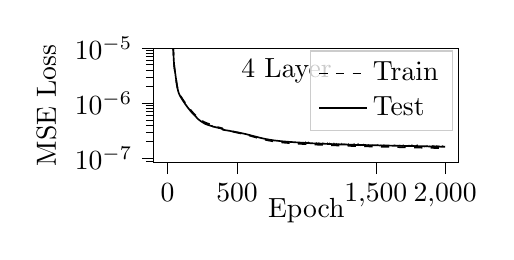
\begin{tikzpicture}

\begin{axis}[
legend cell align={left},
legend style={fill opacity=0.8, draw opacity=1, text opacity=1, draw=white!80!black},
log basis y={10},
tick align=outside,
tick pos=left,
title={4 Layer $\rare$},
title style={at={(0.45,0.85)},anchor=north},
x grid style={white!69.0196078431373!black},
xlabel={Epoch},
x label style={yshift=10pt},
xmin=-99.95, xmax=2098.95,
xtick style={color=black},
xtick = {0,500,1500,2000},
y grid style={white!69.0196078431373!black},
ylabel={MSE Loss},
ymin=8.43938809238065e-08, ymax=1e-5,
ymode=log,
ytick style={color=black},
width=.45\textwidth,
height=.25\textwidth
]
\addplot [semithick, black, dashed]
table {%
0 0.0216106624007225
1 0.00673290289845318
2 0.00242847194336355
3 0.00139278739271685
4 0.000877979734446853
5 0.000474738540826365
6 0.000281054378283443
7 0.00021271777068614
8 0.000184169041807763
9 0.000169510987921967
10 0.000160570089246903
11 0.000153623172860534
12 0.000146821876085596
13 0.000139312337923911
14 0.000130708834607503
15 0.000120814576126577
16 0.000109637301975454
17 9.74004520030576e-05
18 8.46704687937745e-05
19 7.22209239793301e-05
20 6.08980650031299e-05
21 5.13222632107499e-05
22 4.36849454090407e-05
23 3.78588456642319e-05
24 3.35587738209142e-05
25 3.04345663553249e-05
26 2.81585673401423e-05
27 2.64713321785166e-05
28 2.51700294393231e-05
29 2.40990629854423e-05
30 2.31376955125597e-05
31 2.21966665994842e-05
32 2.12135114788907e-05
33 2.01455304168121e-05
34 1.89702411180406e-05
35 1.76808702226481e-05
36 1.62871305710723e-05
37 1.48123448534534e-05
38 1.32958351109664e-05
39 1.17858424450787e-05
40 1.0341288148993e-05
41 9.02308400145557e-06
42 7.88079028029642e-06
43 6.9382161775593e-06
44 6.18492073954258e-06
45 5.61335765496551e-06
46 5.18214040664589e-06
47 4.851168252344e-06
48 4.5908486360986e-06
49 4.37404542492459e-06
50 4.1860971711003e-06
51 4.01634194429334e-06
52 3.85815369747888e-06
53 3.70789047474318e-06
54 3.56210532618206e-06
55 3.42163359334791e-06
56 3.28623007618489e-06
57 3.15185335739443e-06
58 3.0234138083074e-06
59 2.90046724973081e-06
60 2.78323152656412e-06
61 2.67022930574967e-06
62 2.56325708880922e-06
63 2.46282143962162e-06
64 2.36972090749532e-06
65 2.28372049502923e-06
66 2.20383440972682e-06
67 2.12981607876372e-06
68 2.0617129700895e-06
69 1.99959229286151e-06
70 1.94295511562359e-06
71 1.89111669618569e-06
72 1.84340184341636e-06
73 1.79986060237525e-06
74 1.75956733130533e-06
75 1.72281113952977e-06
76 1.68883256932872e-06
77 1.65757721526916e-06
78 1.62893817480381e-06
79 1.60244528660769e-06
80 1.57779333051167e-06
81 1.55488546303673e-06
82 1.53347499124834e-06
83 1.51332984992791e-06
84 1.49426139915931e-06
85 1.47615350221031e-06
86 1.45896057071582e-06
87 1.44265126846221e-06
88 1.42635903176824e-06
89 1.41095506359079e-06
90 1.39608382190204e-06
91 1.38187484546393e-06
92 1.3679947178673e-06
93 1.35463125761248e-06
94 1.34165614971948e-06
95 1.32878456537355e-06
96 1.31631478626559e-06
97 1.30407440371982e-06
98 1.29206818090211e-06
99 1.28030122669998e-06
100 1.26874039784752e-06
101 1.25744272938277e-06
102 1.24637065587763e-06
103 1.23556529459279e-06
104 1.22468484934757e-06
105 1.21391777702229e-06
106 1.20343351045449e-06
107 1.19293890546146e-06
108 1.18257735414318e-06
109 1.17147049024879e-06
110 1.16113315289113e-06
111 1.15103359098612e-06
112 1.14106687107096e-06
113 1.13130547171636e-06
114 1.12164716841789e-06
115 1.11212452972609e-06
116 1.10274103678876e-06
117 1.09347531545723e-06
118 1.08429839545465e-06
119 1.07525509415041e-06
120 1.06630471557878e-06
121 1.05751132139176e-06
122 1.0487439832616e-06
123 1.04011279623251e-06
124 1.03160096955435e-06
125 1.02322621967232e-06
126 1.01492625211108e-06
127 1.00679528438263e-06
128 9.98749102421925e-07
129 9.90614294664738e-07
130 9.82658809448367e-07
131 9.74852750289301e-07
132 9.67159750558721e-07
133 9.59597950853208e-07
134 9.52112600600685e-07
135 9.4466021650419e-07
136 9.37624845334994e-07
137 9.30101956882368e-07
138 9.2261810858929e-07
139 9.15006883133174e-07
140 9.07406760788376e-07
141 9.00099601224724e-07
142 8.92701309766153e-07
143 8.85610241880386e-07
144 8.78771238845388e-07
145 8.72219110959804e-07
146 8.65594072266163e-07
147 8.59149445574303e-07
148 8.52838356223629e-07
149 8.46545972649437e-07
150 8.40331516357651e-07
151 8.34286911057802e-07
152 8.28214898177748e-07
153 8.22116376156146e-07
154 8.16204172863877e-07
155 8.10378548209201e-07
156 8.04656332050513e-07
157 7.99051991762667e-07
158 7.93543244043349e-07
159 7.88110822099952e-07
160 7.82816938922792e-07
161 7.77351807641935e-07
162 7.72005825297129e-07
163 7.66674001397405e-07
164 7.61450602340119e-07
165 7.56337212166613e-07
166 7.5132788563792e-07
167 7.46323605710586e-07
168 7.41613327960522e-07
169 7.36650454257415e-07
170 7.31902793432937e-07
171 7.27025475512733e-07
172 7.22359442249854e-07
173 7.177709151307e-07
174 7.13255188415474e-07
175 7.08742484775371e-07
176 7.03956646006532e-07
177 6.98618378038418e-07
178 6.93606436271921e-07
179 6.88884985976301e-07
180 6.84381060153783e-07
181 6.80145616499317e-07
182 6.75724589797255e-07
183 6.71580819329165e-07
184 6.6738621748641e-07
185 6.6328372876967e-07
186 6.59295098714097e-07
187 6.55370623690032e-07
188 6.51456420968088e-07
189 6.4768271292337e-07
190 6.43534997621487e-07
191 6.39708978283693e-07
192 6.359301758323e-07
193 6.32180300485175e-07
194 6.28438367741069e-07
195 6.24702582612713e-07
196 6.21174068299979e-07
197 6.17387885085918e-07
198 6.1360695735857e-07
199 6.09839239018584e-07
200 6.06011450102528e-07
201 6.02128856996842e-07
202 5.98357907904301e-07
203 5.9438991659988e-07
204 5.90488967759484e-07
205 5.86552403930796e-07
206 5.82735191478889e-07
207 5.7880083262063e-07
208 5.7500634336094e-07
209 5.71188780483567e-07
210 5.67494936362323e-07
211 5.63854762901883e-07
212 5.60381861106407e-07
213 5.57017742153221e-07
214 5.53732854783107e-07
215 5.50645551413709e-07
216 5.47619643711528e-07
217 5.44531466303511e-07
218 5.41552928794431e-07
219 5.38660903046662e-07
220 5.35860492874463e-07
221 5.33061054838413e-07
222 5.30413544254316e-07
223 5.27592542923117e-07
224 5.25051639684193e-07
225 5.22539969892932e-07
226 5.20097590815283e-07
227 5.17746779479467e-07
228 5.15497621826455e-07
229 5.13201537245322e-07
230 5.10952482173366e-07
231 5.08788757684897e-07
232 5.06413795463345e-07
233 5.04197328794476e-07
234 5.02117503565103e-07
235 5.00099920714092e-07
236 4.98156201281574e-07
237 4.96120355620633e-07
238 4.94286574834746e-07
239 4.92361857155288e-07
240 4.90496158661813e-07
241 4.88675696999508e-07
242 4.86913171407366e-07
243 4.851756119848e-07
244 4.83470957902909e-07
245 4.81814274188253e-07
246 4.80199573651419e-07
247 4.78683203567698e-07
248 4.77044099817192e-07
249 4.75468882626728e-07
250 4.73879091153151e-07
251 4.72371058982901e-07
252 4.70842513635716e-07
253 4.6937632956201e-07
254 4.67929217776941e-07
255 4.66513790627232e-07
256 4.65088764485699e-07
257 4.6366257139141e-07
258 4.62334256909003e-07
259 4.60908514426706e-07
260 4.59539256539188e-07
261 4.582419610486e-07
262 4.56966788391355e-07
263 4.55675070149653e-07
264 4.54337393499316e-07
265 4.53071155732232e-07
266 4.51853715723871e-07
267 4.50666905862818e-07
268 4.49487872209886e-07
269 4.48350553412524e-07
270 4.47203686391617e-07
271 4.46084542019776e-07
272 4.44943811899634e-07
273 4.43894103753451e-07
274 4.42781260545644e-07
275 4.4177846840654e-07
276 4.40752303987324e-07
277 4.3963250649881e-07
278 4.38508849981645e-07
279 4.37525406496775e-07
280 4.36493751188038e-07
281 4.35531963482561e-07
282 4.34462244669476e-07
283 4.33431620805891e-07
284 4.32435458542102e-07
285 4.31482845442588e-07
286 4.30554591901e-07
287 4.29638015788214e-07
288 4.28745323013402e-07
289 4.2790234015655e-07
290 4.27039721159872e-07
291 4.26191598307923e-07
292 4.25355553360873e-07
293 4.24506018333659e-07
294 4.23655542931556e-07
295 4.22808301834721e-07
296 4.21996215266063e-07
297 4.21198938262535e-07
298 4.20371942965403e-07
299 4.19587211652583e-07
300 4.18860521804731e-07
301 4.18094755104903e-07
302 4.17349502271236e-07
303 4.16623433551422e-07
304 4.15895910307995e-07
305 4.15184494542586e-07
306 4.14479024385628e-07
307 4.13734667318977e-07
308 4.13033298542587e-07
309 4.12367151128024e-07
310 4.11671337289476e-07
311 4.11018487042725e-07
312 4.10363574829375e-07
313 4.09771400768477e-07
314 4.09135555258899e-07
315 4.08534289007889e-07
316 4.07766801657772e-07
317 4.07205162758828e-07
318 4.06719284313795e-07
319 4.05979226258069e-07
320 4.05369681857337e-07
321 4.04813660580317e-07
322 4.0424221703006e-07
323 4.01775835342733e-07
324 3.9732308940188e-07
325 3.95490883548177e-07
326 3.93727580572545e-07
327 3.9239304535954e-07
328 3.91342631729685e-07
329 3.90330171711639e-07
330 3.89447076273086e-07
331 3.88699826885386e-07
332 3.87784748724584e-07
333 3.87108554747329e-07
334 3.86313853951492e-07
335 3.85547236177786e-07
336 3.84728025963454e-07
337 3.83967091067916e-07
338 3.83136319840105e-07
339 3.82331433002037e-07
340 3.81500545188373e-07
341 3.80685198756225e-07
342 3.80033054341311e-07
343 3.79316259142115e-07
344 3.78621012487201e-07
345 3.7795977845434e-07
346 3.77288775951001e-07
347 3.76653722184983e-07
348 3.75958665728149e-07
349 3.75355292362656e-07
350 3.74698903961246e-07
351 3.74061793934288e-07
352 3.73468358191076e-07
353 3.72811548963625e-07
354 3.72241171824328e-07
355 3.71634515659025e-07
356 3.70998225157848e-07
357 3.70405478889779e-07
358 3.69798000349419e-07
359 3.69194266880868e-07
360 3.68567208624881e-07
361 3.679934441152e-07
362 3.67422204163859e-07
363 3.66914002796648e-07
364 3.66252508641196e-07
365 3.65631194782168e-07
366 3.65033643291213e-07
367 3.6445641813998e-07
368 3.63884713749485e-07
369 3.6333000007005e-07
370 3.62738613333136e-07
371 3.62184976779645e-07
372 3.61609488692238e-07
373 3.61079528076402e-07
374 3.60510225192456e-07
375 3.59959687756373e-07
376 3.59414541676983e-07
377 3.58882117126313e-07
378 3.58320710986959e-07
379 3.57816574023673e-07
380 3.5727768839422e-07
381 3.56719101432645e-07
382 3.56145097327953e-07
383 3.55607541536074e-07
384 3.55104071616097e-07
385 3.54350894710365e-07
386 3.53832532411502e-07
387 3.53362483537012e-07
388 3.52820708798163e-07
389 3.52301250558185e-07
390 3.51839069267612e-07
391 3.51369276515356e-07
392 3.50713634929889e-07
393 3.50198180385064e-07
394 3.42994273879071e-07
395 3.37459253060501e-07
396 3.36289835345838e-07
397 3.35470516276359e-07
398 3.34717947012564e-07
399 3.34036376955282e-07
400 3.33413894921364e-07
401 3.32775672802654e-07
402 3.32222780471625e-07
403 3.31656370008204e-07
404 3.31059441123216e-07
405 3.30471022579104e-07
406 3.29948070614705e-07
407 3.29408178927793e-07
408 3.28830659569235e-07
409 3.28420155582876e-07
410 3.27948691108304e-07
411 3.27466074267591e-07
412 3.26983534591818e-07
413 3.26529947187737e-07
414 3.26056213680204e-07
415 3.25601777944939e-07
416 3.25140297491089e-07
417 3.24708497444703e-07
418 3.24223424328807e-07
419 3.23786114506675e-07
420 3.23332559105438e-07
421 3.22898877939792e-07
422 3.22457123729691e-07
423 3.22002698311508e-07
424 3.21506677451566e-07
425 3.21149641436591e-07
426 3.2071827259017e-07
427 3.20318631850114e-07
428 3.19890345039653e-07
429 3.19473695739703e-07
430 3.18698119528449e-07
431 3.18401096876642e-07
432 3.17974057793435e-07
433 3.17500140937454e-07
434 3.17058012129223e-07
435 3.16648788057705e-07
436 3.16250691852815e-07
437 3.15829835571435e-07
438 3.15423972210738e-07
439 3.15066943116449e-07
440 3.14667640367361e-07
441 3.14271113822429e-07
442 3.13797254975157e-07
443 3.13497316142275e-07
444 3.13078043916448e-07
445 3.12755185831293e-07
446 3.12391271933166e-07
447 3.1198606302496e-07
448 3.1160391039009e-07
449 3.11256480088673e-07
450 3.10887099558954e-07
451 3.10662238675263e-07
452 3.10277672426196e-07
453 3.09896373551055e-07
454 3.09517824987893e-07
455 3.09143135638124e-07
456 3.08770616982201e-07
457 3.08405447086102e-07
458 3.08032719928519e-07
459 3.07656596632455e-07
460 3.07311306372071e-07
461 3.06948595408585e-07
462 3.06615132117827e-07
463 3.06262616817321e-07
464 3.05897978648773e-07
465 3.05542331858533e-07
466 3.05163595825775e-07
467 3.04796437418986e-07
468 3.04440751691004e-07
469 3.04076373026874e-07
470 3.03719222827681e-07
471 3.03353062221845e-07
472 3.02990892649291e-07
473 3.0263301108846e-07
474 3.02271752175898e-07
475 3.01934635672296e-07
476 3.0156328080011e-07
477 3.01179149317932e-07
478 3.00842650105437e-07
479 3.00472060928314e-07
480 3.00037528703001e-07
481 2.99667246835611e-07
482 2.99302288965464e-07
483 2.98947667644711e-07
484 2.98582195583208e-07
485 2.98215010573699e-07
486 2.9785535068072e-07
487 2.97490581374404e-07
488 2.97126231615152e-07
489 2.96774992690985e-07
490 2.96397045090657e-07
491 2.96061390230307e-07
492 2.95681678281312e-07
493 2.9532954511069e-07
494 2.94962441074631e-07
495 2.94596214985177e-07
496 2.94228129320118e-07
497 2.93864728405424e-07
498 2.93508675170528e-07
499 2.93143504279669e-07
500 2.92784303780991e-07
501 2.92416588507649e-07
502 2.92051301343577e-07
503 2.91686755957699e-07
504 2.91287320621336e-07
505 2.90917487433262e-07
506 2.90549759711212e-07
507 2.90181204320561e-07
508 2.89812056109895e-07
509 2.89444514450565e-07
510 2.89075045500908e-07
511 2.88704543976337e-07
512 2.88336096332387e-07
513 2.8796272732734e-07
514 2.87592303521933e-07
515 2.87219270418859e-07
516 2.86848664543982e-07
517 2.86476573634786e-07
518 2.86102311221725e-07
519 2.85724018624478e-07
520 2.85357762265903e-07
521 2.84981645876314e-07
522 2.8461455055151e-07
523 2.8425328021342e-07
524 2.83887521433712e-07
525 2.83510480073801e-07
526 2.83132329769842e-07
527 2.82761600246317e-07
528 2.82383754637294e-07
529 2.82003369363792e-07
530 2.81624365769062e-07
531 2.81253791044378e-07
532 2.80863522320374e-07
533 2.80491489519363e-07
534 2.80108860522432e-07
535 2.79729500917369e-07
536 2.79344856437547e-07
537 2.78964073430643e-07
538 2.78581386027099e-07
539 2.78189427277198e-07
540 2.77800684699514e-07
541 2.77422164160157e-07
542 2.77025935531583e-07
543 2.76675719604214e-07
544 2.7628835702842e-07
545 2.75891499214254e-07
546 2.754996529859e-07
547 2.7510834667055e-07
548 2.7471418212599e-07
549 2.74250312244817e-07
550 2.73937980210803e-07
551 2.73469895518019e-07
552 2.73089561275697e-07
553 2.72698263458437e-07
554 2.72312604806757e-07
555 2.71926184367999e-07
556 2.71536050803434e-07
557 2.71139314662605e-07
558 2.70746581449544e-07
559 2.70352984330202e-07
560 2.69956387015213e-07
561 2.69561034599519e-07
562 2.69184922245813e-07
563 2.68785443537922e-07
564 2.68388820202858e-07
565 2.67988743360092e-07
566 2.67580664214506e-07
567 2.6718646597601e-07
568 2.66785075979215e-07
569 2.66419031149212e-07
570 2.66015551616761e-07
571 2.65620774769104e-07
572 2.65219328838384e-07
573 2.64824864359525e-07
574 2.64434130130553e-07
575 2.64023973286953e-07
576 2.63620257200614e-07
577 2.63219747282051e-07
578 2.62736836447175e-07
579 2.62318192085331e-07
580 2.61909523416648e-07
581 2.61502716469408e-07
582 2.61105529247629e-07
583 2.60702718719585e-07
584 2.6029890841528e-07
585 2.59889832378235e-07
586 2.59486747424376e-07
587 2.59076840677608e-07
588 2.58672434839013e-07
589 2.58264190520663e-07
590 2.57854916384304e-07
591 2.57446017087659e-07
592 2.57047310228131e-07
593 2.56630037597461e-07
594 2.56229556200083e-07
595 2.55818167815391e-07
596 2.55413956594452e-07
597 2.55009213333324e-07
598 2.54611830413864e-07
599 2.54200633449386e-07
600 2.5380529264396e-07
601 2.53393371764332e-07
602 2.52922564399682e-07
603 2.52380531748031e-07
604 2.51938129494533e-07
605 2.5150760473025e-07
606 2.51107723556743e-07
607 2.50692401550623e-07
608 2.50296422933616e-07
609 2.49886340895955e-07
610 2.49492911265747e-07
611 2.49087333429543e-07
612 2.48680714250327e-07
613 2.48284265978782e-07
614 2.4788667600717e-07
615 2.47456508517985e-07
616 2.47051033085199e-07
617 2.46647489134944e-07
618 2.4625732633865e-07
619 2.45860469803461e-07
620 2.45425408920141e-07
621 2.45022914640458e-07
622 2.44652590524197e-07
623 2.44252181644811e-07
624 2.43862469332612e-07
625 2.43488337133613e-07
626 2.43087162303368e-07
627 2.42683210387895e-07
628 2.42284148342264e-07
629 2.4189684177145e-07
630 2.41453110305656e-07
631 2.4105597925228e-07
632 2.40666493098729e-07
633 2.402901326235e-07
634 2.39877828683177e-07
635 2.39510399850928e-07
636 2.39118784641335e-07
637 2.38734965940068e-07
638 2.38333517231126e-07
639 2.37971021149974e-07
640 2.37577484739404e-07
641 2.37201121635167e-07
642 2.36807600217048e-07
643 2.36442187372177e-07
644 2.36048477418649e-07
645 2.35720507248516e-07
646 2.3529685198298e-07
647 2.34926964964188e-07
648 2.34651763484806e-07
649 2.34295619804925e-07
650 2.33907534919808e-07
651 2.33553717706059e-07
652 2.33175521088924e-07
653 2.32825393268854e-07
654 2.32450461304268e-07
655 2.32095179185876e-07
656 2.31748523042086e-07
657 2.31385499631642e-07
658 2.31015129955381e-07
659 2.30663613251636e-07
660 2.30288796053912e-07
661 2.29934373187746e-07
662 2.29571597571976e-07
663 2.29216760359918e-07
664 2.28852116933354e-07
665 2.28495701144027e-07
666 2.28147498418707e-07
667 2.27798743303254e-07
668 2.27462652588883e-07
669 2.27117970155177e-07
670 2.26760281407223e-07
671 2.26418564309938e-07
672 2.26108651581569e-07
673 2.25791860522406e-07
674 2.25436486502417e-07
675 2.25098220347775e-07
676 2.24788045336766e-07
677 2.24459609604821e-07
678 2.24133774658242e-07
679 2.23800147416853e-07
680 2.23474523565415e-07
681 2.23188974956656e-07
682 2.2284166180242e-07
683 2.2254372058228e-07
684 2.22211433126063e-07
685 2.21920742731641e-07
686 2.21595553426823e-07
687 2.21314227367486e-07
688 2.21033817595639e-07
689 2.20716097487639e-07
690 2.20356926739385e-07
691 2.2009933127265e-07
692 2.19786205256867e-07
693 2.19499166888681e-07
694 2.19210622162791e-07
695 2.18931428264568e-07
696 2.18612988660993e-07
697 2.18332271472832e-07
698 2.18054914128629e-07
699 2.17747560832038e-07
700 2.17494242413352e-07
701 2.17189853188415e-07
702 2.16910481917409e-07
703 2.16647721089203e-07
704 2.16394595852876e-07
705 2.1610913848491e-07
706 2.15835460842584e-07
707 2.15616975424382e-07
708 2.15359850656682e-07
709 2.15075565435541e-07
710 2.14831694350437e-07
711 2.14503112900388e-07
712 2.14279591034483e-07
713 2.13987736259469e-07
714 2.13740835725673e-07
715 2.13455635510229e-07
716 2.13242247525614e-07
717 2.12986595641951e-07
718 2.12713128561859e-07
719 2.12486485366981e-07
720 2.12225340455063e-07
721 2.11995605106097e-07
722 2.11794130493104e-07
723 2.11524806914554e-07
724 2.1125673990241e-07
725 2.11031820846586e-07
726 2.1081890638186e-07
727 2.10560273671945e-07
728 2.10315091813129e-07
729 2.10102463988449e-07
730 2.09889895714355e-07
731 2.09609642865871e-07
732 2.09425779999606e-07
733 2.09183616597386e-07
734 2.08990658443042e-07
735 2.08729989289225e-07
736 2.08531867073702e-07
737 2.08309944277119e-07
738 2.08086278355779e-07
739 2.0789459659909e-07
740 2.07680310651881e-07
741 2.0747119165776e-07
742 2.07236777498565e-07
743 2.07018175132134e-07
744 2.06816486773675e-07
745 2.06584763589035e-07
746 2.06387027432697e-07
747 2.06218926180668e-07
748 2.06005806859366e-07
749 2.05752826182959e-07
750 2.05548594330196e-07
751 2.05311775921757e-07
752 2.05142609736697e-07
753 2.0495073572846e-07
754 2.04771630293976e-07
755 2.0461071154898e-07
756 2.04373782693779e-07
757 2.04192100383693e-07
758 2.04031139503513e-07
759 2.03814531289481e-07
760 2.03654313601476e-07
761 2.03442323652325e-07
762 2.03277292598614e-07
763 2.0309212533931e-07
764 2.02949136372865e-07
765 2.02724689088996e-07
766 2.02560473084645e-07
767 2.02350404919116e-07
768 2.02225088422381e-07
769 2.02075813668046e-07
770 2.01815807457706e-07
771 2.01668591600423e-07
772 2.01510255024573e-07
773 2.01304897409216e-07
774 2.01147469894636e-07
775 2.0087547069636e-07
776 2.00708041205644e-07
777 2.00552844987101e-07
778 2.00407669666447e-07
779 2.00212583891357e-07
780 2.00079323661839e-07
781 1.99906171182818e-07
782 1.99735537769641e-07
783 1.99590529170734e-07
784 1.99458949076359e-07
785 1.9929100927385e-07
786 1.99101222690956e-07
787 1.98979387548093e-07
788 1.9883520160846e-07
789 1.98662458501531e-07
790 1.98509994092433e-07
791 1.98378701213642e-07
792 1.98230722041615e-07
793 1.98054001302239e-07
794 1.97913957400431e-07
795 1.97748915866214e-07
796 1.97619246243619e-07
797 1.97458854394483e-07
798 1.9732037737441e-07
799 1.9718832942317e-07
800 1.97041426808653e-07
801 1.96902047633785e-07
802 1.96766920048219e-07
803 1.96604294650626e-07
804 1.96496536219115e-07
805 1.96382572973164e-07
806 1.96219839480705e-07
807 1.96085320837369e-07
808 1.95963470162042e-07
809 1.95823555152685e-07
810 1.95713456996316e-07
811 1.95573616785794e-07
812 1.95453819671343e-07
813 1.95311064544512e-07
814 1.95212965564906e-07
815 1.95100162919459e-07
816 1.94962750249772e-07
817 1.94830665954271e-07
818 1.94717411517331e-07
819 1.94620832374426e-07
820 1.94458740004677e-07
821 1.94354109922301e-07
822 1.94270007597197e-07
823 1.94124745341639e-07
824 1.94010768659325e-07
825 1.93872416154761e-07
826 1.93788308628484e-07
827 1.93651885346924e-07
828 1.93532121421924e-07
829 1.93444749363891e-07
830 1.93306050924491e-07
831 1.93204075095821e-07
832 1.9309011060642e-07
833 1.92993874705394e-07
834 1.92862723380927e-07
835 1.92772320488643e-07
836 1.92665639630718e-07
837 1.92546770804825e-07
838 1.92435405381275e-07
839 1.92352559281517e-07
840 1.92240041741343e-07
841 1.92133511006887e-07
842 1.92020548425376e-07
843 1.919115628084e-07
844 1.91812710554018e-07
845 1.91718293251597e-07
846 1.91616724755761e-07
847 1.91497081054592e-07
848 1.91413476578362e-07
849 1.91311501069436e-07
850 1.91188739904646e-07
851 1.91130697771769e-07
852 1.91013988590782e-07
853 1.90901197811399e-07
854 1.90812814622632e-07
855 1.90715631696037e-07
856 1.90646210654677e-07
857 1.90514590059365e-07
858 1.90444030131687e-07
859 1.90331704054358e-07
860 1.90250029120875e-07
861 1.90143055029068e-07
862 1.90024863513827e-07
863 1.89974942529147e-07
864 1.89862021365173e-07
865 1.89752594678794e-07
866 1.89691171975426e-07
867 1.89590054446853e-07
868 1.89481359015531e-07
869 1.89564498441541e-07
870 1.89266790783904e-07
871 1.89147045318805e-07
872 1.89083462664996e-07
873 1.89025151307476e-07
874 1.88914466036749e-07
875 1.88806591928881e-07
876 1.88748112037729e-07
877 1.88681913918742e-07
878 1.88565463105306e-07
879 1.88473345332341e-07
880 1.88422301071967e-07
881 1.88273862789856e-07
882 1.88229817830177e-07
883 1.88129125866965e-07
884 1.88074489372525e-07
885 1.87977990435684e-07
886 1.87873305492303e-07
887 1.87809109206682e-07
888 1.87705275983774e-07
889 1.87653425115286e-07
890 1.87576660152899e-07
891 1.87455449136564e-07
892 1.8739126468148e-07
893 1.87289279985237e-07
894 1.8724850141183e-07
895 1.87153168901943e-07
896 1.8706308216565e-07
897 1.86987817727413e-07
898 1.86928051377322e-07
899 1.86846638250415e-07
900 1.86764167771969e-07
901 1.86676254728013e-07
902 1.86577274298827e-07
903 1.86536912949009e-07
904 1.8646056668814e-07
905 1.86386593952648e-07
906 1.86291404176586e-07
907 1.86223032379473e-07
908 1.86134376484404e-07
909 1.86082618697014e-07
910 1.85978073758974e-07
911 1.85938494226434e-07
912 1.85864153408488e-07
913 1.85785363839841e-07
914 1.85678791211785e-07
915 1.85629285340383e-07
916 1.85553920864834e-07
917 1.85486233405641e-07
918 1.8540947337442e-07
919 1.85350580267141e-07
920 1.85271162948197e-07
921 1.85202297849685e-07
922 1.85131175925335e-07
923 1.85051926912649e-07
924 1.84978863472907e-07
925 1.8492998484021e-07
926 1.84832688674419e-07
927 1.84801209300645e-07
928 1.84736455373979e-07
929 1.84623548165064e-07
930 1.84608434793176e-07
931 1.84504162469068e-07
932 1.84435943999972e-07
933 1.84360517607729e-07
934 1.84322198350628e-07
935 1.84215514472896e-07
936 1.84190147251684e-07
937 1.84140666071642e-07
938 1.84041638341625e-07
939 1.83968719234429e-07
940 1.83896355849811e-07
941 1.83837361070971e-07
942 1.83839822845755e-07
943 1.83766977229993e-07
944 1.83638415258258e-07
945 1.83566072095687e-07
946 1.83519504091123e-07
947 1.83446028835021e-07
948 1.83395068596326e-07
949 1.83316212236662e-07
950 1.83285562606272e-07
951 1.83199140721513e-07
952 1.83183291241562e-07
953 1.83075190882676e-07
954 1.83062210787455e-07
955 1.82927106422426e-07
956 1.82892595525175e-07
957 1.82834764522966e-07
958 1.82783786037533e-07
959 1.82701763108639e-07
960 1.82646872232795e-07
961 1.82573253077578e-07
962 1.82511307478705e-07
963 1.82460096070258e-07
964 1.82422018170314e-07
965 1.82331821022785e-07
966 1.82296495310652e-07
967 1.82236372658906e-07
968 1.8213447961557e-07
969 1.8208163304223e-07
970 1.82025621178639e-07
971 1.81966136040046e-07
972 1.81946712665138e-07
973 1.81872313675058e-07
974 1.81773238892902e-07
975 1.81758913051056e-07
976 1.8167523741397e-07
977 1.81603671109087e-07
978 1.81574254867201e-07
979 1.81481448350951e-07
980 1.8144391169983e-07
981 1.81378839940294e-07
982 1.81291478270396e-07
983 1.81267837923826e-07
984 1.81212172982725e-07
985 1.81145498459045e-07
986 1.81104971638035e-07
987 1.81015536654172e-07
988 1.81003275883995e-07
989 1.80951426081322e-07
990 1.80898478369329e-07
991 1.80804848220362e-07
992 1.80737904678097e-07
993 1.80692982183928e-07
994 1.8063039879479e-07
995 1.80686602881508e-07
996 1.80568369920309e-07
997 1.80461264832843e-07
998 1.80398518651259e-07
999 1.80379310890544e-07
1000 1.80326845374168e-07
1001 1.80228571188934e-07
1002 1.80212151668968e-07
1003 1.80164973421881e-07
1004 1.80055146493885e-07
1005 1.80016070551403e-07
1006 1.80035480369156e-07
1007 1.79911012459399e-07
1008 1.79842733800228e-07
1009 1.79833708145338e-07
1010 1.79744951807947e-07
1011 1.79718168539011e-07
1012 1.79695514212597e-07
1013 1.79632579659028e-07
1014 1.7958827668707e-07
1015 1.79485900808629e-07
1016 1.79413860877276e-07
1017 1.79370492290332e-07
1018 1.79360341761026e-07
1019 1.79332420671585e-07
1020 1.79230263661623e-07
1021 1.7917569885384e-07
1022 1.79127057556627e-07
1023 1.79241113549722e-07
1024 1.7917623971897e-07
1025 1.79244382202626e-07
1026 1.79210308260735e-07
1027 1.79150409216788e-07
1028 1.79036714634151e-07
1029 1.79027852738045e-07
1030 1.78958927357087e-07
1031 1.7893335813568e-07
1032 1.78864548978197e-07
1033 1.78835367890429e-07
1034 1.78795579536484e-07
1035 1.78755134868425e-07
1036 1.78641936344093e-07
1037 1.78593477691891e-07
1038 1.78590952224056e-07
1039 1.78499820442823e-07
1040 1.78439640791339e-07
1041 1.78394428537842e-07
1042 1.78378901708243e-07
1043 1.78302251427453e-07
1044 1.78258820334065e-07
1045 1.78191099934111e-07
1046 1.78159377298925e-07
1047 1.78104258438339e-07
1048 1.78057871373483e-07
1049 1.78015181447222e-07
1050 1.77944034774669e-07
1051 1.77941957588246e-07
1052 1.77853626396995e-07
1053 1.77814524832343e-07
1054 1.7774813699134e-07
1055 1.77703809889351e-07
1056 1.77675952258483e-07
1057 1.77648358352656e-07
1058 1.77571942579391e-07
1059 1.77527472061456e-07
1060 1.77485991635251e-07
1061 1.7744707773204e-07
1062 1.77386032802929e-07
1063 1.77322587973094e-07
1064 1.77299124445085e-07
1065 1.77234235543722e-07
1066 1.77215259405727e-07
1067 1.77158344335737e-07
1068 1.77124247471738e-07
1069 1.77064489179202e-07
1070 1.76985912368366e-07
1071 1.76983701834388e-07
1072 1.76910187533963e-07
1073 1.76876028099571e-07
1074 1.76824726956681e-07
1075 1.76798676029932e-07
1076 1.76776226531672e-07
1077 1.76694430521707e-07
1078 1.76621351180017e-07
1079 1.76610401460664e-07
1080 1.76574187129575e-07
1081 1.7649910562767e-07
1082 1.76468546882802e-07
1083 1.76431862030313e-07
1084 1.7638737516279e-07
1085 1.76306908748813e-07
1086 1.76277939857528e-07
1087 1.76302373539272e-07
1088 1.7617569829298e-07
1089 1.76178361300572e-07
1090 1.76133429633296e-07
1091 1.76041002141858e-07
1092 1.75977817043815e-07
1093 1.75944437359021e-07
1094 1.75941254248357e-07
1095 1.75881839190595e-07
1096 1.75846790924084e-07
1097 1.75819223144913e-07
1098 1.75713790490306e-07
1099 1.75664444050483e-07
1100 1.75637258344352e-07
1101 1.75566675693517e-07
1102 1.75534115825826e-07
1103 1.75526750261668e-07
1104 1.75438703770681e-07
1105 1.7538309885623e-07
1106 1.75376762328483e-07
1107 1.7530193790094e-07
1108 1.75282633335883e-07
1109 1.75220648891639e-07
1110 1.75184468702128e-07
1111 1.75177809552451e-07
1112 1.75096959537768e-07
1113 1.75071028550633e-07
1114 1.75022347598031e-07
1115 1.7497661561805e-07
1116 1.74940363855569e-07
1117 1.74892061075127e-07
1118 1.74832643715206e-07
1119 1.74859169668196e-07
1120 1.74774426554336e-07
1121 1.7468253720665e-07
1122 1.74662733201103e-07
1123 1.74636310930509e-07
1124 1.74569058856378e-07
1125 1.74553399908461e-07
1126 1.74507346848429e-07
1127 1.74474903275268e-07
1128 1.74449821827238e-07
1129 1.74340132559792e-07
1130 1.74361761217767e-07
1131 1.74297626386988e-07
1132 1.74214229467395e-07
1133 1.74233699652859e-07
1134 1.7419528980156e-07
1135 1.74113174260526e-07
1136 1.74103606482845e-07
1137 1.74103460260255e-07
1138 1.73959555390013e-07
1139 1.73925013555731e-07
1140 1.7386210139847e-07
1141 1.73848528262965e-07
1142 1.73805815336436e-07
1143 1.73731946027544e-07
1144 1.73736144176928e-07
1145 1.73698482896612e-07
1146 1.73662524865392e-07
1147 1.73587405967623e-07
1148 1.73579918822497e-07
1149 1.73576758577099e-07
1150 1.735323319636e-07
1151 1.73485661129291e-07
1152 1.73443705548948e-07
1153 1.73351196750104e-07
1154 1.73381033533815e-07
1155 1.73310837986662e-07
1156 1.73295372221105e-07
1157 1.73259445723772e-07
1158 1.73227503879048e-07
1159 1.73195007207028e-07
1160 1.73187520424278e-07
1161 1.7306360564362e-07
1162 1.73050464432833e-07
1163 1.73035037157376e-07
1164 1.73087016712259e-07
1165 1.72968198214107e-07
1166 1.72881617530152e-07
1167 1.7295136483142e-07
1168 1.72851830512855e-07
1169 1.72818079022363e-07
1170 1.72778573158894e-07
1171 1.72718693640661e-07
1172 1.7270090534538e-07
1173 1.7270916892187e-07
1174 1.72568362536651e-07
1175 1.72577032891752e-07
1176 1.7258109477325e-07
1177 1.7260609226355e-07
1178 1.72448717250973e-07
1179 1.72415710743223e-07
1180 1.72395935955194e-07
1181 1.72397184961426e-07
1182 1.72349606657463e-07
1183 1.72301530355412e-07
1184 1.72214634403645e-07
1185 1.72153765760186e-07
1186 1.72193612456795e-07
1187 1.72204249409447e-07
1188 1.72087060846593e-07
1189 1.72026658063373e-07
1190 1.72075992630027e-07
1191 1.72030504209886e-07
1192 1.71926870820016e-07
1193 1.71936961912422e-07
1194 1.71891174524319e-07
1195 1.71880935219804e-07
1196 1.71827827792015e-07
1197 1.71822777382147e-07
1198 1.71786435757326e-07
1199 1.71768815185658e-07
1200 1.71702090860038e-07
1201 1.71739857854902e-07
1202 1.71617547074732e-07
1203 1.7156320400602e-07
1204 1.71528990875913e-07
1205 1.71517066888782e-07
1206 1.71513961973346e-07
1207 1.71403330170961e-07
1208 1.71346198889921e-07
1209 1.71383523543511e-07
1210 1.71362682102938e-07
1211 1.71336470835115e-07
1212 1.71251969312891e-07
1213 1.71174495115167e-07
1214 1.71233604270071e-07
1215 1.71314036798265e-07
1216 1.71165501981818e-07
1217 1.71071120618649e-07
1218 1.70984958153042e-07
1219 1.7098195895926e-07
1220 1.71015771975647e-07
1221 1.70996565053372e-07
1222 1.70884112144165e-07
1223 1.7089750729582e-07
1224 1.70790641050189e-07
1225 1.70798408198891e-07
1226 1.70828165650505e-07
1227 1.70793065173314e-07
1228 1.70700528443035e-07
1229 1.7067476072441e-07
1230 1.70675086287986e-07
1231 1.70612983040996e-07
1232 1.70565547598756e-07
1233 1.7050324265e-07
1234 1.70488775488309e-07
1235 1.70464546236815e-07
1236 1.70451107408098e-07
1237 1.70438943598583e-07
1238 1.70367497503321e-07
1239 1.70297669853881e-07
1240 1.70287840084882e-07
1241 1.70317440392864e-07
1242 1.70259187768806e-07
1243 1.70169387097019e-07
1244 1.70166060954102e-07
1245 1.7015959914346e-07
1246 1.70072879036809e-07
1247 1.70080203453438e-07
1248 1.69973099353626e-07
1249 1.70045703136168e-07
1250 1.69952917950411e-07
1251 1.69955662016719e-07
1252 1.69859973333075e-07
1253 1.69899801925055e-07
1254 1.69820288007827e-07
1255 1.69868564412923e-07
1256 1.69765343969175e-07
1257 1.69748448229257e-07
1258 1.69705800452391e-07
1259 1.6965306291894e-07
1260 1.69602442973371e-07
1261 1.69608080632599e-07
1262 1.69599682138255e-07
1263 1.69567798202763e-07
1264 1.69505588857533e-07
1265 1.69445060365092e-07
1266 1.69388760596689e-07
1267 1.69400478604587e-07
1268 1.69410320395968e-07
1269 1.69311620716428e-07
1270 1.69259400074395e-07
1271 1.69325856880675e-07
1272 1.69370852745487e-07
1273 1.69243204737768e-07
1274 1.69179619966542e-07
1275 1.69161871589552e-07
1276 1.69083306850837e-07
1277 1.69077230957271e-07
1278 1.69089837299907e-07
1279 1.69023000928803e-07
1280 1.69091059262882e-07
1281 1.68983588977767e-07
1282 1.68936555738242e-07
1283 1.68931953034246e-07
1284 1.68985705300884e-07
1285 1.68975296190865e-07
1286 1.68837971287417e-07
1287 1.68774838392949e-07
1288 1.68735167370926e-07
1289 1.68765960466999e-07
1290 1.68746516699514e-07
1291 1.68695649733763e-07
1292 1.68646468864608e-07
1293 1.68562413257689e-07
1294 1.6858988993107e-07
1295 1.68670126527104e-07
1296 1.68366325972613e-07
1297 1.6832450091897e-07
1298 1.68334291473116e-07
1299 1.68343839312968e-07
1300 1.68317190968992e-07
1301 1.68235172893105e-07
1302 1.68274554212644e-07
1303 1.68399181184498e-07
1304 1.68282554334098e-07
1305 1.68080057100894e-07
1306 1.68025432877528e-07
1307 1.68044797234757e-07
1308 1.68017354866379e-07
1309 1.67995841799495e-07
1310 1.68006798560327e-07
1311 1.67982508379794e-07
1312 1.67921054860187e-07
1313 1.67883917420397e-07
1314 1.67839464054964e-07
1315 1.67829756712479e-07
1316 1.67853974403442e-07
1317 1.67749433863662e-07
1318 1.67708428286062e-07
1319 1.67713444042761e-07
1320 1.67860712927848e-07
1321 1.67689125817105e-07
1322 1.67559621274904e-07
1323 1.67547872322871e-07
1324 1.67564348146243e-07
1325 1.67477222703383e-07
1326 1.67485049338723e-07
1327 1.67526131981788e-07
1328 1.6742998275987e-07
1329 1.67414902726648e-07
1330 1.6736702631448e-07
1331 1.67352104973872e-07
1332 1.67339367976638e-07
1333 1.6726915405485e-07
1334 1.67304407696633e-07
1335 1.67264324431926e-07
1336 1.67214283322892e-07
1337 1.67262341591368e-07
1338 1.67241847648825e-07
1339 1.67110093784117e-07
1340 1.67036057391101e-07
1341 1.67139857801146e-07
1342 1.67201785750137e-07
1343 1.66920922900715e-07
1344 1.66950420755541e-07
1345 1.66943121350016e-07
1346 1.66929704967345e-07
1347 1.66912089149207e-07
1348 1.66969160659392e-07
1349 1.66813377553865e-07
1350 1.66787883031816e-07
1351 1.66778691990999e-07
1352 1.66794166055695e-07
1353 1.66790056709942e-07
1354 1.66844713575642e-07
1355 1.66592245811614e-07
1356 1.66663042314497e-07
1357 1.66594229689565e-07
1358 1.66581775118857e-07
1359 1.66553394748803e-07
1360 1.66581533129317e-07
1361 1.66522043343775e-07
1362 1.66457377808626e-07
1363 1.66468092778871e-07
1364 1.66456248294367e-07
1365 1.66391937916899e-07
1366 1.6636954207172e-07
1367 1.66337186605858e-07
1368 1.66337999544908e-07
1369 1.66300411265752e-07
1370 1.66256585025337e-07
1371 1.66230324694538e-07
1372 1.66262054960953e-07
1373 1.66311842029643e-07
1374 1.6620884812113e-07
1375 1.66082737052875e-07
1376 1.66100138692116e-07
1377 1.66071855289829e-07
1378 1.65991287140343e-07
1379 1.66027292841875e-07
1380 1.66048765017024e-07
1381 1.65978204798023e-07
1382 1.65909461287583e-07
1383 1.65914692715319e-07
1384 1.65921796678958e-07
1385 1.65908610057386e-07
1386 1.6584075878967e-07
1387 1.65783007716414e-07
1388 1.65777221020846e-07
1389 1.65749755105082e-07
1390 1.65692761413538e-07
1391 1.65716249071579e-07
1392 1.65707926868208e-07
1393 1.65664443692037e-07
1394 1.65660392909217e-07
1395 1.6555531041007e-07
1396 1.65595974486621e-07
1397 1.65527711487812e-07
1398 1.65510852603745e-07
1399 1.65448139732405e-07
1400 1.65507440037516e-07
1401 1.65409376414516e-07
1402 1.65359866144854e-07
1403 1.65365921347416e-07
1404 1.65365050953881e-07
1405 1.65445104364892e-07
1406 1.65383935843977e-07
1407 1.65204668604702e-07
1408 1.65154134542433e-07
1409 1.65219209932843e-07
1410 1.65202215775651e-07
1411 1.6515671573103e-07
1412 1.65137949920791e-07
1413 1.65116417022659e-07
1414 1.6504532810302e-07
1415 1.65028859363758e-07
1416 1.6504706556475e-07
1417 1.64975679453505e-07
1418 1.64952036158184e-07
1419 1.64949861805042e-07
1420 1.64942287014469e-07
1421 1.64880639310638e-07
1422 1.64852907623469e-07
1423 1.64815023296683e-07
1424 1.64827068971363e-07
1425 1.6479692638427e-07
1426 1.64800686256683e-07
1427 1.64663229007544e-07
1428 1.64735067940569e-07
1429 1.64699877252872e-07
1430 1.64645984632727e-07
1431 1.64649042353915e-07
1432 1.64592018414567e-07
1433 1.64586802981148e-07
1434 1.64533369286346e-07
1435 1.64534088234802e-07
1436 1.64539180580903e-07
1437 1.64588025249657e-07
1438 1.64528626413585e-07
1439 1.64403049730311e-07
1440 1.64434569235539e-07
1441 1.64330305665317e-07
1442 1.64350557383841e-07
1443 1.64313907802693e-07
1444 1.64288167425752e-07
1445 1.64290333536599e-07
1446 1.64252259480691e-07
1447 1.64279479896834e-07
1448 1.6423641449137e-07
1449 1.64184464686912e-07
1450 1.64129400964441e-07
1451 1.64106395708075e-07
1452 1.64089033887649e-07
1453 1.64048898746216e-07
1454 1.64055080958292e-07
1455 1.64035842338706e-07
1456 1.64035157851572e-07
1457 1.63966343592392e-07
1458 1.6393386583502e-07
1459 1.63920002862028e-07
1460 1.63905486353144e-07
1461 1.63842626747623e-07
1462 1.63854071125513e-07
1463 1.63843182377832e-07
1464 1.63801519676099e-07
1465 1.63759081736714e-07
1466 1.63764028513924e-07
1467 1.63723978161556e-07
1468 1.63663750292642e-07
1469 1.63675580736822e-07
1470 1.63701325028853e-07
1471 1.63652787477986e-07
1472 1.63594848658022e-07
1473 1.63543358503659e-07
1474 1.63574874825656e-07
1475 1.63533181869013e-07
1476 1.63477860958494e-07
1477 1.63506070094854e-07
1478 1.6346910118159e-07
1479 1.63388968786649e-07
1480 1.63403992630151e-07
1481 1.63401504394756e-07
1482 1.63334911896129e-07
1483 1.63362521405475e-07
1484 1.63307964221815e-07
1485 1.63266157784392e-07
1486 1.63244747525937e-07
1487 1.63252576001582e-07
1488 1.63205464630778e-07
1489 1.6317926982623e-07
1490 1.63177952131832e-07
1491 1.63116752538883e-07
1492 1.63130517712773e-07
1493 1.63142071770039e-07
1494 1.63082057653696e-07
1495 1.63039829530476e-07
1496 1.62986418189348e-07
1497 1.63003632266623e-07
1498 1.6297419497846e-07
1499 1.62977809573306e-07
1500 1.62908251610361e-07
1501 1.62888266856953e-07
1502 1.62894972540073e-07
1503 1.6281705941168e-07
1504 1.62824144119611e-07
1505 1.62801411775604e-07
1506 1.62785903242479e-07
1507 1.62790458873019e-07
1508 1.62755779378188e-07
1509 1.62805195941473e-07
1510 1.62741083300943e-07
1511 1.62614733277167e-07
1512 1.62588511336992e-07
1513 1.62593399018363e-07
1514 1.62582695779179e-07
1515 1.62611406956614e-07
1516 1.62567546233561e-07
1517 1.62476563382086e-07
1518 1.62453610897728e-07
1519 1.62472841758188e-07
1520 1.62409258251728e-07
1521 1.62407369678874e-07
1522 1.62439174310691e-07
1523 1.62376711131174e-07
1524 1.62357890829412e-07
1525 1.62330951390288e-07
1526 1.62282029890548e-07
1527 1.62258464939669e-07
1528 1.62386171474793e-07
1529 1.62246081977457e-07
1530 1.62181757545454e-07
1531 1.6214893717148e-07
1532 1.62138087752339e-07
1533 1.6213818561539e-07
1534 1.62098755609463e-07
1535 1.62070517177426e-07
1536 1.62076942373801e-07
1537 1.62076044901482e-07
1538 1.62060141597919e-07
1539 1.61987526915652e-07
1540 1.61971739032651e-07
1541 1.61926232046028e-07
1542 1.61918721609311e-07
1543 1.61893961497128e-07
1544 1.6187512852639e-07
1545 1.61897783129916e-07
1546 1.6183849820095e-07
1547 1.61819013932529e-07
1548 1.61767674043745e-07
1549 1.61779257460637e-07
1550 1.61762891366379e-07
1551 1.61720912878138e-07
1552 1.61708021494178e-07
1553 1.61623495422702e-07
1554 1.61689888656724e-07
1555 1.61645654770837e-07
1556 1.61627561659827e-07
1557 1.61584144386495e-07
1558 1.61566055083995e-07
1559 1.61593238935609e-07
1560 1.6156369655107e-07
1561 1.61485519804216e-07
1562 1.6143838396232e-07
1563 1.61465926417748e-07
1564 1.61439363473903e-07
1565 1.61373608236204e-07
1566 1.61376746753206e-07
1567 1.61372395311332e-07
1568 1.61365052711915e-07
1569 1.61270477434528e-07
1570 1.61305438325599e-07
1571 1.6128386074854e-07
1572 1.6120980218659e-07
1573 1.61217556552629e-07
1574 1.61202849270126e-07
1575 1.61158415636464e-07
1576 1.61146072542806e-07
1577 1.61116594973976e-07
1578 1.61089867823705e-07
1579 1.61058869643682e-07
1580 1.61075818958523e-07
1581 1.60997869258495e-07
1582 1.60995202037384e-07
1583 1.60991695985047e-07
1584 1.60972638340695e-07
1585 1.60917201000643e-07
1586 1.60925989412419e-07
1587 1.6090620315623e-07
1588 1.60876287630174e-07
1589 1.60871587006284e-07
1590 1.608295123674e-07
1591 1.60810746869799e-07
1592 1.60792823564293e-07
1593 1.60731222976551e-07
1594 1.60725678398421e-07
1595 1.60743065173108e-07
1596 1.60692538059948e-07
1597 1.60662292991276e-07
1598 1.60687539874971e-07
1599 1.60647360310406e-07
1600 1.60643607117095e-07
1601 1.60562668689579e-07
1602 1.60560070440852e-07
1603 1.60531671774322e-07
1604 1.605189931837e-07
1605 1.60465122299058e-07
1606 1.60481532560652e-07
1607 1.60452848923853e-07
1608 1.60447297758992e-07
1609 1.60448149877368e-07
1610 1.60383949321385e-07
1611 1.60370203410309e-07
1612 1.60340380546131e-07
1613 1.60316806301353e-07
1614 1.60336975469022e-07
1615 1.60274468434807e-07
1616 1.60265671610205e-07
1617 1.60206146965436e-07
1618 1.6017395471124e-07
1619 1.6019242134746e-07
1620 1.60202111970875e-07
1621 1.60110613911968e-07
1622 1.60101618185138e-07
1623 1.60084186518361e-07
1624 1.60075974164897e-07
1625 1.60056341130144e-07
1626 1.60024469295195e-07
1627 1.60016861734391e-07
1628 1.5996215306302e-07
1629 1.59993971742267e-07
1630 1.59975415030544e-07
1631 1.59897546794241e-07
1632 1.59864979707436e-07
1633 1.5981264795073e-07
1634 1.59833385943386e-07
1635 1.59786259438022e-07
1636 1.5975959943404e-07
1637 1.59836109965283e-07
1638 1.59749508142681e-07
1639 1.59673018117701e-07
1640 1.59672461165883e-07
1641 1.59673905095303e-07
1642 1.59624695783123e-07
1643 1.59605662418016e-07
1644 1.59605513445626e-07
1645 1.59538471798726e-07
1646 1.59518216165111e-07
1647 1.59490265389195e-07
1648 1.59514611830502e-07
1649 1.59506289037381e-07
1650 1.594392940234e-07
1651 1.59437268926865e-07
1652 1.59391223355954e-07
1653 1.59379607872268e-07
1654 1.5933557291703e-07
1655 1.59336109298636e-07
1656 1.59273247241742e-07
1657 1.59280083103397e-07
1658 1.59303168210556e-07
1659 1.59266005447023e-07
1660 1.5923947286467e-07
1661 1.59195379566768e-07
1662 1.59185277276208e-07
1663 1.59162616085951e-07
1664 1.59113985738202e-07
1665 1.59115515032227e-07
1666 1.59078035096627e-07
1667 1.590620035401e-07
1668 1.59055500247973e-07
1669 1.59017629734137e-07
1670 1.59004733653489e-07
1671 1.58984582405708e-07
1672 1.5893618891738e-07
1673 1.58970893295418e-07
1674 1.58974270824785e-07
1675 1.58856075486824e-07
1676 1.58825552816211e-07
1677 1.5882929874067e-07
1678 1.58840414911765e-07
1679 1.58816994570543e-07
1680 1.58759385541885e-07
1681 1.58741842831489e-07
1682 1.587232752982e-07
1683 1.58727088788169e-07
1684 1.5868284273779e-07
1685 1.58663293703398e-07
1686 1.58653893663541e-07
1687 1.58617259465643e-07
1688 1.58564271245609e-07
1689 1.58562940306695e-07
1690 1.5858223643761e-07
1691 1.58529176921718e-07
1692 1.58498967628873e-07
1693 1.58529810825314e-07
1694 1.58439630631335e-07
1695 1.58456428877685e-07
1696 1.58413188358963e-07
1697 1.58366994817527e-07
1698 1.5844551713684e-07
1699 1.58414659182426e-07
1700 1.58323922740067e-07
1701 1.58267001054924e-07
1702 1.58278427797143e-07
1703 1.5828589792477e-07
1704 1.58217034922359e-07
1705 1.58233597289836e-07
1706 1.58217247403059e-07
1707 1.58180190943824e-07
1708 1.58171623702685e-07
1709 1.58144930544779e-07
1710 1.5814085011101e-07
1711 1.5810550590345e-07
1712 1.58071546813687e-07
1713 1.58090500818275e-07
1714 1.5802699835632e-07
1715 1.58003030328757e-07
1716 1.57996284798401e-07
1717 1.57944636079321e-07
1718 1.57902301893387e-07
1719 1.57958363530497e-07
1720 1.57928429686649e-07
1721 1.5788781043824e-07
1722 1.5786845246879e-07
1723 1.57857515972637e-07
1724 1.57811574084121e-07
1725 1.57765941366961e-07
1726 1.57808763667333e-07
1727 1.57781808809432e-07
1728 1.57732858816928e-07
1729 1.57714919623686e-07
1730 1.57751770103687e-07
1731 1.57683196277958e-07
1732 1.57685341640956e-07
1733 1.57640333512177e-07
1734 1.57593496886932e-07
1735 1.57609387201774e-07
1736 1.57577048810253e-07
1737 1.57558252041667e-07
1738 1.57547913936185e-07
1739 1.57577006746124e-07
1740 1.57516168158622e-07
1741 1.57490005882721e-07
1742 1.57429037734857e-07
1743 1.57414762966823e-07
1744 1.57409189966984e-07
1745 1.57392864515771e-07
1746 1.57372618552642e-07
1747 1.57369900080084e-07
1748 1.57315704235828e-07
1749 1.57344287217143e-07
1750 1.57322670489179e-07
1751 1.57240089080801e-07
1752 1.57292073694748e-07
1753 1.57229541215997e-07
1754 1.5717209772248e-07
1755 1.57209250694734e-07
1756 1.57179648994088e-07
1757 1.57179907695593e-07
1758 1.57142846951785e-07
1759 1.57105183667738e-07
1760 1.57075447177135e-07
1761 1.57090822746397e-07
1762 1.57044919340876e-07
1763 1.57105361083154e-07
1764 1.57034673691214e-07
1765 1.56961065272299e-07
1766 1.57016002901855e-07
1767 1.56986994667818e-07
1768 1.56888791920551e-07
1769 1.56876593472077e-07
1770 1.56917016937541e-07
1771 1.56922129733061e-07
1772 1.56847977351049e-07
1773 1.56800327566486e-07
1774 1.5682984567178e-07
1775 1.56779214854907e-07
1776 1.56776219405685e-07
1777 1.56752019925932e-07
1778 1.5677984612239e-07
1779 1.56721015706296e-07
1780 1.56645402846323e-07
1781 1.56664259037598e-07
1782 1.5669497613402e-07
1783 1.56634603719397e-07
1784 1.56614299477553e-07
1785 1.56558301490861e-07
1786 1.56580395156425e-07
1787 1.56591386783589e-07
1788 1.5655352395072e-07
1789 1.56526596931883e-07
1790 1.56484596296025e-07
1791 1.56495141503399e-07
1792 1.56515446228411e-07
1793 1.56453958460645e-07
1794 1.5640798075367e-07
1795 1.56401567515729e-07
1796 1.56359416891405e-07
1797 1.56362065531823e-07
1798 1.56313302149158e-07
1799 1.56343904500034e-07
1800 1.56341277055105e-07
1801 1.56306155076891e-07
1802 1.56228445597151e-07
1803 1.56236447892866e-07
1804 1.56230175768712e-07
1805 1.56186808865755e-07
1806 1.5617487574815e-07
1807 1.56168291802317e-07
1808 1.56181358271112e-07
1809 1.56139952530054e-07
1810 1.56133709339201e-07
1811 1.56110389013975e-07
1812 1.56057965199352e-07
1813 1.56061774760019e-07
1814 1.56010338500323e-07
1815 1.56005747960819e-07
1816 1.56006777984885e-07
1817 1.56005831996708e-07
1818 1.55922724239588e-07
1819 1.55939529996374e-07
1820 1.55891446091516e-07
1821 1.55887576582359e-07
1822 1.5586792800093e-07
1823 1.55863338093809e-07
1824 1.55858713945634e-07
1825 1.55812652685938e-07
1826 1.55833806914529e-07
1827 1.55781838373059e-07
1828 1.55788733756879e-07
1829 1.55721982039836e-07
1830 1.55727386349724e-07
1831 1.55851433291332e-07
1832 1.55649586091045e-07
1833 1.55669927124791e-07
1834 1.55658901377365e-07
1835 1.55604411197885e-07
1836 1.55595658576146e-07
1837 1.55614966381279e-07
1838 1.5569612568811e-07
1839 1.5562331170571e-07
1840 1.55492145026415e-07
1841 1.55512192719698e-07
1842 1.55482258158202e-07
1843 1.55477846043084e-07
1844 1.5547972850527e-07
1845 1.55428200905305e-07
1846 1.55491830078347e-07
1847 1.55435238333723e-07
1848 1.55356304126997e-07
1849 1.55355119474621e-07
1850 1.55342363079569e-07
1851 1.55484200355716e-07
1852 1.55344910034216e-07
1853 1.55267062737607e-07
1854 1.55249093879206e-07
1855 1.55265172224972e-07
1856 1.55231461768324e-07
1857 1.55227018687754e-07
1858 1.55229627608833e-07
1859 1.55182650459551e-07
1860 1.55232340787848e-07
1861 1.55126972622099e-07
1862 1.55099817320092e-07
1863 1.55121186253382e-07
1864 1.5512751639335e-07
1865 1.55050447901317e-07
1866 1.55049290604836e-07
1867 1.55044010597294e-07
1868 1.55025785332441e-07
1869 1.55098577394597e-07
1870 1.54999461358329e-07
1871 1.54985007675634e-07
1872 1.54967518348315e-07
1873 1.54887229378176e-07
1874 1.54899446044965e-07
1875 1.54890364761684e-07
1876 1.5493079467177e-07
1877 1.54870422015563e-07
1878 1.54849424923498e-07
1879 1.54797378826288e-07
1880 1.54824989564872e-07
1881 1.54811023548973e-07
1882 1.54755810577001e-07
1883 1.54771308856994e-07
1884 1.54729633891293e-07
1885 1.54714625892893e-07
1886 1.54732818650416e-07
1887 1.54677888644983e-07
1888 1.54708835552242e-07
1889 1.54635840303285e-07
1890 1.54602401082116e-07
1891 1.54665540129884e-07
1892 1.54590238217622e-07
1893 1.54579007322297e-07
1894 1.54548660638909e-07
1895 1.54497419629251e-07
1896 1.54537538065824e-07
1897 1.54494466642063e-07
1898 1.54535719360638e-07
1899 1.54445405819104e-07
1900 1.5440485092455e-07
1901 1.54465775601409e-07
1902 1.54365925610023e-07
1903 1.54361977244832e-07
1904 1.54492287371966e-07
1905 1.54350942509041e-07
1906 1.54304357273816e-07
1907 1.54337254919312e-07
1908 1.54339452990371e-07
1909 1.54368744645694e-07
1910 1.54261017364377e-07
1911 1.5425102045441e-07
1912 1.54197756522478e-07
1913 1.54183083964199e-07
1914 1.54233713530516e-07
1915 1.54137876023697e-07
1916 1.54145033270936e-07
1917 1.54135794069532e-07
1918 1.54119535679342e-07
1919 1.54138514481872e-07
1920 1.54096629827905e-07
1921 1.5406265574569e-07
1922 1.54060015155721e-07
1923 1.54024330797142e-07
1924 1.54051954218915e-07
1925 1.54064928601372e-07
1926 1.53961385088053e-07
1927 1.53930946780179e-07
1928 1.53962987965883e-07
1929 1.53929885584603e-07
1930 1.53935032173536e-07
1931 1.53870435326553e-07
1932 1.53908900053068e-07
1933 1.53856674970143e-07
1934 1.53846832844806e-07
1935 1.53875489658617e-07
1936 1.53802510780565e-07
1937 1.53803029697031e-07
1938 1.53788990317594e-07
1939 1.537533772904e-07
1940 1.53762179159855e-07
1941 1.53716116081171e-07
1942 1.53707295403649e-07
1943 1.53690711535148e-07
1944 1.53655579865131e-07
1945 1.53632156518313e-07
1946 1.53633985100043e-07
1947 1.53624035995392e-07
1948 1.53726699338108e-07
1949 1.53600323478997e-07
1950 1.53522084893609e-07
1951 1.53526479572008e-07
1952 1.53521940212897e-07
1953 1.53634212182396e-07
1954 1.53472079396977e-07
1955 1.53470182361559e-07
1956 1.53480214308388e-07
1957 1.5347605283722e-07
1958 1.53418531354532e-07
1959 1.53409420832418e-07
1960 1.53398752225087e-07
1961 1.5340143021092e-07
1962 1.53342927447397e-07
1963 1.53396333921307e-07
1964 1.53329097088317e-07
1965 1.53354786689874e-07
1966 1.53264965028654e-07
1967 1.53241224921885e-07
1968 1.53321128870232e-07
1969 1.53190591866803e-07
1970 1.53264055889224e-07
1971 1.53205914649845e-07
1972 1.5320671469965e-07
1973 1.53186781268744e-07
1974 1.53127663807595e-07
1975 1.53145490287443e-07
1976 1.53173064497025e-07
1977 1.53088147015978e-07
1978 1.53112812604661e-07
1979 1.53141912839772e-07
1980 1.53054309471656e-07
1981 1.52986316905412e-07
1982 1.52974265290595e-07
1983 1.52974430363884e-07
1984 1.52938154521109e-07
1985 1.52912020645601e-07
1986 1.52903801485138e-07
1987 1.5294464648008e-07
1988 1.52980406049608e-07
1989 1.52853272858522e-07
1990 1.52853196887293e-07
1991 1.52872027200601e-07
1992 1.52813105628979e-07
1993 1.5282282419804e-07
1994 1.52767130309428e-07
1995 1.52762753117486e-07
1996 1.52713809200122e-07
1997 1.52790601468666e-07
1998 1.52704478431076e-07
1999 1.52719887466901e-07
};
\addlegendentry{Train}
\addplot [semithick, black]
table {%
0 0.011574000120163
1 0.00366706307977438
2 0.00170789565891027
3 0.00111751689109951
4 0.000646881584543735
5 0.000352886680047959
6 0.000245284551056102
7 0.000204639916773885
8 0.000184964592335746
9 0.000173768785316497
10 0.000165942328749225
11 0.000158926923177205
12 0.000151453103171661
13 0.000142998978844844
14 0.000133258625282906
15 0.00012215982133057
16 0.000109797903860454
17 9.66031366260722e-05
18 8.32770165288821e-05
19 7.07173239788972e-05
20 5.97596590523608e-05
21 5.08381381223444e-05
22 4.38926981587429e-05
23 3.86942701879889e-05
24 3.48979883710854e-05
25 3.21265833918005e-05
26 3.00821902783355e-05
27 2.85236837953562e-05
28 2.72683046205202e-05
29 2.61690584011376e-05
30 2.51223918894539e-05
31 2.40484914684203e-05
32 2.28933586186031e-05
33 2.16249518416589e-05
34 2.02315659407759e-05
35 1.87114783329889e-05
36 1.70845323737012e-05
37 1.53870423673652e-05
38 1.36686712721712e-05
39 1.19934302347247e-05
40 1.04305418062722e-05
41 9.04368243936915e-06
42 7.8759376265225e-06
43 6.92470666763256e-06
44 6.19254478806397e-06
45 5.6361955103057e-06
46 5.21145375387277e-06
47 4.87881288790959e-06
48 4.61657509731594e-06
49 4.3916338654526e-06
50 4.20265496359207e-06
51 4.03814738092478e-06
52 3.88146781915566e-06
53 3.73240868611902e-06
54 3.5890325307264e-06
55 3.45053081218794e-06
56 3.31653723151248e-06
57 3.180617113685e-06
58 3.04861714539584e-06
59 2.92030449600134e-06
60 2.7996170501865e-06
61 2.68204576059361e-06
62 2.57092233368894e-06
63 2.46800846070983e-06
64 2.37122208091023e-06
65 2.28195494855754e-06
66 2.20259494199126e-06
67 2.12626673601335e-06
68 2.05498326977249e-06
69 1.98996053768496e-06
70 1.93037385542993e-06
71 1.87562704923039e-06
72 1.82363464773516e-06
73 1.77665367573354e-06
74 1.73253715729516e-06
75 1.69225052104593e-06
76 1.6553547084186e-06
77 1.62138883297303e-06
78 1.59035300839605e-06
79 1.56235898884916e-06
80 1.53617838805076e-06
81 1.51190454289463e-06
82 1.48939363953104e-06
83 1.46829404457094e-06
84 1.44854095651681e-06
85 1.43001614105742e-06
86 1.41249040552793e-06
87 1.39639860208263e-06
88 1.38081929890177e-06
89 1.36582798404561e-06
90 1.3515806358555e-06
91 1.33778735289525e-06
92 1.3242972727312e-06
93 1.31096430777689e-06
94 1.2978662198293e-06
95 1.2850188113589e-06
96 1.27255157167383e-06
97 1.26033637570799e-06
98 1.24842938475922e-06
99 1.23707002330775e-06
100 1.22564551929827e-06
101 1.21429775390425e-06
102 1.20332890674035e-06
103 1.1918360769414e-06
104 1.18086018119357e-06
105 1.17003378363734e-06
106 1.15892203211843e-06
107 1.14825797936646e-06
108 1.13600242457323e-06
109 1.12509349037282e-06
110 1.11494068733009e-06
111 1.10509256501246e-06
112 1.09550103388756e-06
113 1.08612948679365e-06
114 1.07696200757346e-06
115 1.0678922990337e-06
116 1.05891751900344e-06
117 1.0499041991352e-06
118 1.04081368590414e-06
119 1.03180457244889e-06
120 1.02287845038518e-06
121 1.01399359664356e-06
122 1.0052174275188e-06
123 9.9669341580011e-07
124 9.88451802186319e-07
125 9.80408231043839e-07
126 9.72623865891364e-07
127 9.64914420364948e-07
128 9.57318775363092e-07
129 9.49509797010251e-07
130 9.41864186643215e-07
131 9.34281558784278e-07
132 9.26734685435804e-07
133 9.19426440759707e-07
134 9.12015252652054e-07
135 9.04922842437372e-07
136 8.97438610536483e-07
137 8.90073920345458e-07
138 8.82843323779525e-07
139 8.75568218816625e-07
140 8.68446079493879e-07
141 8.61326327594725e-07
142 8.54532061111968e-07
143 8.48092724936578e-07
144 8.41753944769152e-07
145 8.35587854908226e-07
146 8.29325244922074e-07
147 8.23131017568812e-07
148 8.17043883216684e-07
149 8.1094850656882e-07
150 8.04856426839251e-07
151 7.99804638518253e-07
152 7.93898664142034e-07
153 7.88029069553886e-07
154 7.81995822762838e-07
155 7.76178239902947e-07
156 7.70457518228795e-07
157 7.64824449106527e-07
158 7.59258000471164e-07
159 7.53204631109838e-07
160 7.47757894714596e-07
161 7.42383235774469e-07
162 7.37123684757535e-07
163 7.3189210070268e-07
164 7.26665348338429e-07
165 7.21628850897105e-07
166 7.16773115527758e-07
167 7.1098833132055e-07
168 7.06490709490026e-07
169 7.02067382007954e-07
170 6.97423786277795e-07
171 6.93051902089792e-07
172 6.88729130615684e-07
173 6.8440965605987e-07
174 6.79950119319983e-07
175 6.75605576816452e-07
176 6.70747397180094e-07
177 6.65254674458993e-07
178 6.60655985029734e-07
179 6.56397730836034e-07
180 6.52389530841901e-07
181 6.48681634629611e-07
182 6.45296154289099e-07
183 6.41551309854549e-07
184 6.38289577636897e-07
185 6.34649552466726e-07
186 6.31188356692292e-07
187 6.26032715445035e-07
188 6.23962023382774e-07
189 6.20240598436794e-07
190 6.16676913978154e-07
191 6.13114991665498e-07
192 6.09508276738779e-07
193 6.06156334015395e-07
194 6.02723559950391e-07
195 6.00569137532148e-07
196 5.97140285663045e-07
197 5.93776462665119e-07
198 5.90396894040168e-07
199 5.86575083616481e-07
200 5.82730763198924e-07
201 5.78846595544746e-07
202 5.74758303173439e-07
203 5.71062741983042e-07
204 5.6730300457275e-07
205 5.63755065741134e-07
206 5.60191267595656e-07
207 5.56695908926486e-07
208 5.53021493487904e-07
209 5.47904960512824e-07
210 5.44347074082907e-07
211 5.41051235813939e-07
212 5.37774440090288e-07
213 5.3457591775441e-07
214 5.31512796442257e-07
215 5.28517830389319e-07
216 5.25565894804458e-07
217 5.22576385719731e-07
218 5.19615412031271e-07
219 5.16793988936115e-07
220 5.13939539814601e-07
221 5.11242149059399e-07
222 5.08597054249549e-07
223 5.06128117194748e-07
224 5.0382772087687e-07
225 5.01570184496813e-07
226 4.99327484249079e-07
227 4.97108032959659e-07
228 4.94572248044278e-07
229 4.92386675432499e-07
230 4.90237198391696e-07
231 4.88122566366656e-07
232 4.8613941316944e-07
233 4.83994483602146e-07
234 4.82092389120226e-07
235 4.80200071706349e-07
236 4.78123013181175e-07
237 4.76248374070565e-07
238 4.74345398515652e-07
239 4.72492956760107e-07
240 4.70647904649013e-07
241 4.68791654384404e-07
242 4.66988893776943e-07
243 4.65245904024414e-07
244 4.63530795968836e-07
245 4.61884667402046e-07
246 4.60318574369012e-07
247 4.58637714473298e-07
248 4.57168653156259e-07
249 4.54612546718636e-07
250 4.53028235369857e-07
251 4.51211690233322e-07
252 4.4972932755627e-07
253 4.48309435796546e-07
254 4.46909439233423e-07
255 4.45462774223415e-07
256 4.4384333364178e-07
257 4.42337722006414e-07
258 4.40380546251617e-07
259 4.39089689052707e-07
260 4.37857494262062e-07
261 4.366330870198e-07
262 4.35459241998615e-07
263 4.31679268331209e-07
264 4.30122213401773e-07
265 4.28812853670024e-07
266 4.27644152978246e-07
267 4.26482699822373e-07
268 4.25356915911834e-07
269 4.2420649037922e-07
270 4.22662679966379e-07
271 4.21609740897111e-07
272 4.2056589677486e-07
273 4.19518642047478e-07
274 4.18486308717547e-07
275 4.1739392031559e-07
276 4.16438382444539e-07
277 4.15426768540783e-07
278 4.14379883295624e-07
279 4.1346791590513e-07
280 4.12524912007939e-07
281 4.11731662097736e-07
282 4.10663517413923e-07
283 4.0974902049129e-07
284 4.08751930081053e-07
285 4.07973942628814e-07
286 4.07007945568694e-07
287 4.06237774086549e-07
288 4.0542386159359e-07
289 4.04617111371408e-07
290 4.03779665703041e-07
291 4.02873013172211e-07
292 4.01829282736799e-07
293 4.01031030605736e-07
294 4.0031130765783e-07
295 3.99608637735582e-07
296 3.98779576471497e-07
297 3.9822057829042e-07
298 3.97490708792247e-07
299 3.96917897660387e-07
300 3.96119702372744e-07
301 3.95498801708527e-07
302 3.94853771013004e-07
303 3.9425222553291e-07
304 3.93532303633037e-07
305 3.92527141457322e-07
306 3.91253138332104e-07
307 3.90722732390714e-07
308 3.90216598589177e-07
309 3.8958322079452e-07
310 3.88906670423239e-07
311 3.88249361549242e-07
312 3.87616012176295e-07
313 3.87023845860313e-07
314 3.86869260182721e-07
315 3.86024908038962e-07
316 3.85521957468882e-07
317 3.8626055243185e-07
318 3.85887119591644e-07
319 3.85291372140273e-07
320 3.84759573535121e-07
321 3.84187245572321e-07
322 3.83851727292495e-07
323 3.82557658440419e-07
324 3.79693375407442e-07
325 3.78235114339986e-07
326 3.76254604361748e-07
327 3.75335702074153e-07
328 3.74560670479696e-07
329 3.73444891010877e-07
330 3.73139982912107e-07
331 3.72862615449776e-07
332 3.72420856820099e-07
333 3.73164709799312e-07
334 3.73019844346345e-07
335 3.72857385855241e-07
336 3.72445867924398e-07
337 3.71896618389655e-07
338 3.71369708318525e-07
339 3.70636030311289e-07
340 3.70102839042374e-07
341 3.69565583469011e-07
342 3.68768354519489e-07
343 3.68172550224699e-07
344 3.67809093404503e-07
345 3.67119611155431e-07
346 3.66304760746061e-07
347 3.66120275430148e-07
348 3.65379548838973e-07
349 3.65072963859348e-07
350 3.6432285810406e-07
351 3.64246261597145e-07
352 3.63825591875866e-07
353 3.63105527867447e-07
354 3.62947218945919e-07
355 3.62348288263092e-07
356 3.61952089633633e-07
357 3.61228728706919e-07
358 3.60791631237589e-07
359 3.60364708740235e-07
360 3.59777459379984e-07
361 3.5935704545409e-07
362 3.58532417976676e-07
363 3.57953780394382e-07
364 3.57419139618287e-07
365 3.56875688112268e-07
366 3.56552618541173e-07
367 3.55851341282687e-07
368 3.55311158273253e-07
369 3.54814204683862e-07
370 3.54620112830162e-07
371 3.54929824197825e-07
372 3.54227182697286e-07
373 3.53933444330323e-07
374 3.53550319687201e-07
375 3.52759201405206e-07
376 3.52269552195139e-07
377 3.52011284121545e-07
378 3.51253163444198e-07
379 3.51150447386317e-07
380 3.49637161889405e-07
381 3.48938726801862e-07
382 3.48291536056422e-07
383 3.47915374732111e-07
384 3.47847446846572e-07
385 3.47481886819878e-07
386 3.46875168588667e-07
387 3.46714813304061e-07
388 3.46323759004008e-07
389 3.45925883493692e-07
390 3.4565402984299e-07
391 3.45379618238439e-07
392 3.44890224823757e-07
393 3.44146030784032e-07
394 3.36688287916331e-07
395 3.34762262355071e-07
396 3.33707816935203e-07
397 3.32992300400292e-07
398 3.32326521856885e-07
399 3.31464406144732e-07
400 3.31011847265472e-07
401 3.30504462908721e-07
402 3.29830101009065e-07
403 3.29425660083871e-07
404 3.28782817859974e-07
405 3.28433287677399e-07
406 3.27996929172514e-07
407 3.27296447721892e-07
408 3.27268566024941e-07
409 3.26741570688682e-07
410 3.2631803037475e-07
411 3.25972393966367e-07
412 3.25581197557767e-07
413 3.25209157381323e-07
414 3.24919938066159e-07
415 3.24388025774169e-07
416 3.24229290527001e-07
417 3.23735889651289e-07
418 3.23417253866864e-07
419 3.22991155599084e-07
420 3.22784956097166e-07
421 3.22435283806044e-07
422 3.22153937304392e-07
423 3.2172994224311e-07
424 3.21632086297541e-07
425 3.21252741741773e-07
426 3.20962698197036e-07
427 3.20572581813394e-07
428 3.20207647064308e-07
429 3.19756196631715e-07
430 3.19627673661671e-07
431 3.19204815468765e-07
432 3.18889675554601e-07
433 3.18575274604882e-07
434 3.18293984946649e-07
435 3.18343666094734e-07
436 3.17982767228386e-07
437 3.17682406603126e-07
438 3.17364794000241e-07
439 3.16984994697123e-07
440 3.16649732212682e-07
441 3.16126261168392e-07
442 3.16085703389035e-07
443 3.15712867404727e-07
444 3.15370357384381e-07
445 3.15339576673068e-07
446 3.15004001549823e-07
447 3.14620791641573e-07
448 3.14270550916262e-07
449 3.1391988386531e-07
450 3.13089259407207e-07
451 3.12688257508853e-07
452 3.12337419927644e-07
453 3.11977174760614e-07
454 3.11632135208129e-07
455 3.11291870502828e-07
456 3.10953282678383e-07
457 3.10632827904556e-07
458 3.10372001877113e-07
459 3.10032049810616e-07
460 3.09867033365663e-07
461 3.0952986662669e-07
462 3.09208076032519e-07
463 3.08884636979201e-07
464 3.08578222529832e-07
465 3.08301252971432e-07
466 3.08034657336975e-07
467 3.07606256910731e-07
468 3.07291571743917e-07
469 3.06981291942066e-07
470 3.06688605178351e-07
471 3.06369400959738e-07
472 3.06053152598906e-07
473 3.05713712123179e-07
474 3.053798423025e-07
475 3.04861373479071e-07
476 3.05539430200952e-07
477 3.05176399706397e-07
478 3.04749789847847e-07
479 3.04363766190363e-07
480 3.03893244790743e-07
481 3.03489088082642e-07
482 3.03117559496968e-07
483 3.02754301628738e-07
484 3.02415003261558e-07
485 3.02079911307374e-07
486 3.01694171866984e-07
487 3.01341884778594e-07
488 3.0099880632406e-07
489 3.00644757089685e-07
490 3.00288945709326e-07
491 2.99927279456824e-07
492 2.99587242125199e-07
493 2.99238195111684e-07
494 2.98902278927926e-07
495 2.98555534072875e-07
496 2.98258953534969e-07
497 2.97935201842847e-07
498 2.97610142752092e-07
499 2.97283349937061e-07
500 2.96965112056569e-07
501 2.9664417411368e-07
502 2.9630987796736e-07
503 2.9598055562019e-07
504 2.95722486498562e-07
505 2.9538978196797e-07
506 2.95058185884045e-07
507 2.94712322101987e-07
508 2.94369954190188e-07
509 2.94032730607796e-07
510 2.93682688834451e-07
511 2.93338757728634e-07
512 2.92983088456822e-07
513 2.92643278498872e-07
514 2.92304946469812e-07
515 2.91953710984671e-07
516 2.91607619828937e-07
517 2.91251382122937e-07
518 2.90900260324634e-07
519 2.90575172812169e-07
520 2.90223084675745e-07
521 2.89879778847535e-07
522 2.89501599581854e-07
523 2.89185152269056e-07
524 2.88839345330416e-07
525 2.88481629695525e-07
526 2.88134714310218e-07
527 2.87771086959765e-07
528 2.87394243514427e-07
529 2.87049402913908e-07
530 2.86693222051326e-07
531 2.86315412267868e-07
532 2.85956446077762e-07
533 2.85580114223194e-07
534 2.85229361907113e-07
535 2.84853683751862e-07
536 2.84494120705858e-07
537 2.84125604821384e-07
538 2.83870150497023e-07
539 2.83490919628093e-07
540 2.8312533117969e-07
541 2.8274163810238e-07
542 2.82374031712607e-07
543 2.8200162205394e-07
544 2.81621538533727e-07
545 2.81268512480892e-07
546 2.8089388592889e-07
547 2.80520936257744e-07
548 2.80160094234816e-07
549 2.7980559025309e-07
550 2.79421868754071e-07
551 2.79073560705001e-07
552 2.78715475587887e-07
553 2.78348835536235e-07
554 2.78005728659991e-07
555 2.77634768508506e-07
556 2.77269691650872e-07
557 2.768990725599e-07
558 2.76530244036621e-07
559 2.76160193379837e-07
560 2.75797845006309e-07
561 2.75427112228499e-07
562 2.75067179700272e-07
563 2.74701903890673e-07
564 2.7433281957201e-07
565 2.73965270025656e-07
566 2.73609543910425e-07
567 2.73232217296027e-07
568 2.72860347649839e-07
569 2.72434988346504e-07
570 2.72053000571759e-07
571 2.71784244887385e-07
572 2.71395975914857e-07
573 2.71007650098909e-07
574 2.70626401288609e-07
575 2.70254929546354e-07
576 2.69863164703565e-07
577 2.69484672799081e-07
578 2.68867324848543e-07
579 2.68489316113119e-07
580 2.68125802449504e-07
581 2.67730001723976e-07
582 2.67355744654196e-07
583 2.66966026174487e-07
584 2.66580883589995e-07
585 2.66187356601222e-07
586 2.65798206555701e-07
587 2.65406129074108e-07
588 2.65013028410976e-07
589 2.64614101297411e-07
590 2.64223103840777e-07
591 2.63831395841407e-07
592 2.63443297399135e-07
593 2.63062531757896e-07
594 2.62660904581935e-07
595 2.62268031292479e-07
596 2.61867967310536e-07
597 2.61462247408417e-07
598 2.6108338602171e-07
599 2.60689262177038e-07
600 2.60297724707925e-07
601 2.59904197719152e-07
602 2.5932695280062e-07
603 2.58735894931306e-07
604 2.58358767268874e-07
605 2.57999460018254e-07
606 2.57653141488845e-07
607 2.57296079553271e-07
608 2.56944787224711e-07
609 2.56603641446418e-07
610 2.56247972174606e-07
611 2.55876727806026e-07
612 2.55541152682781e-07
613 2.55171727303605e-07
614 2.54801648225111e-07
615 2.54435406077391e-07
616 2.54054526749314e-07
617 2.53687204576636e-07
618 2.53374679459739e-07
619 2.5291257088611e-07
620 2.52521687116314e-07
621 2.52182218218877e-07
622 2.51883733426439e-07
623 2.51409375096046e-07
624 2.510828380764e-07
625 2.50676947644024e-07
626 2.50245761890255e-07
627 2.49866133117393e-07
628 2.49488351755645e-07
629 2.49147149133933e-07
630 2.48713462269734e-07
631 2.48321072149338e-07
632 2.48028442229042e-07
633 2.47545159481888e-07
634 2.47190229174521e-07
635 2.46833224082366e-07
636 2.46446376195308e-07
637 2.46034716155918e-07
638 2.45701102130624e-07
639 2.45358478423441e-07
640 2.44987234054861e-07
641 2.44581343622485e-07
642 2.44356158418668e-07
643 2.43886660200587e-07
644 2.43649793674194e-07
645 2.43248194919943e-07
646 2.42877632672389e-07
647 2.42497151248244e-07
648 2.42231067204557e-07
649 2.41791468624797e-07
650 2.41566596059783e-07
651 2.41110427623425e-07
652 2.40842808807429e-07
653 2.40432285636416e-07
654 2.40140423102275e-07
655 2.39740046481529e-07
656 2.39430335113866e-07
657 2.38958989484672e-07
658 2.38692393850215e-07
659 2.3829443307477e-07
660 2.37951979897844e-07
661 2.37546771586494e-07
662 2.37231517985492e-07
663 2.36864622138455e-07
664 2.36517308849216e-07
665 2.36199028336159e-07
666 2.35781655533174e-07
667 2.35482119137487e-07
668 2.35176500495982e-07
669 2.34811381005784e-07
670 2.3447526587006e-07
671 2.34158619605296e-07
672 2.33794096970996e-07
673 2.33537519989113e-07
674 2.33106590030729e-07
675 2.32907524377879e-07
676 2.3253474523699e-07
677 2.32320743975833e-07
678 2.31974524922407e-07
679 2.31625094215815e-07
680 2.31340337109032e-07
681 2.31092514013653e-07
682 2.30703591341808e-07
683 2.30442054771629e-07
684 2.30081525387504e-07
685 2.29810225960136e-07
686 2.29471496027145e-07
687 2.29219878633558e-07
688 2.28838104021634e-07
689 2.28553830083911e-07
690 2.28224678266997e-07
691 2.27979384703758e-07
692 2.27619921133737e-07
693 2.27384390427687e-07
694 2.27092996851752e-07
695 2.26775085820918e-07
696 2.26479698994808e-07
697 2.26220109311726e-07
698 2.25936602760157e-07
699 2.25703516321119e-07
700 2.254302557958e-07
701 2.25145598165e-07
702 2.24920455593747e-07
703 2.24611724775059e-07
704 2.24347132871117e-07
705 2.2408249833461e-07
706 2.23930527454286e-07
707 2.23703963797561e-07
708 2.23431271706431e-07
709 2.23261721998824e-07
710 2.22965169882627e-07
711 2.22815160100254e-07
712 2.22608775857225e-07
713 2.22415039274892e-07
714 2.22238853098133e-07
715 2.22039901132121e-07
716 2.21726409677103e-07
717 2.21545150225211e-07
718 2.21242103748409e-07
719 2.21089408114494e-07
720 2.20802405692666e-07
721 2.20430663944171e-07
722 2.20185839339138e-07
723 2.1988783771576e-07
724 2.19640952536793e-07
725 2.1947865036509e-07
726 2.19261806932991e-07
727 2.19024485659247e-07
728 2.18756127878805e-07
729 2.18547654640133e-07
730 2.18282409036874e-07
731 2.18030095311406e-07
732 2.17866528373634e-07
733 2.17574907424023e-07
734 2.17409663605395e-07
735 2.1716815012951e-07
736 2.16939668007399e-07
737 2.16778417438945e-07
738 2.1647457515428e-07
739 2.16365833693999e-07
740 2.1602446054203e-07
741 2.15883900978042e-07
742 2.15626442923167e-07
743 2.1546036066411e-07
744 2.15647858681223e-07
745 2.15580712392693e-07
746 2.1533863048262e-07
747 2.15239097656195e-07
748 2.14897241335166e-07
749 2.14720657254475e-07
750 2.14489176642019e-07
751 2.14276852261719e-07
752 2.14003208043323e-07
753 2.13844003837949e-07
754 2.13662602277509e-07
755 2.13403296811521e-07
756 2.13128416248765e-07
757 2.12970675761426e-07
758 2.12726050108358e-07
759 2.12609066352343e-07
760 2.12377727848434e-07
761 2.12120355058687e-07
762 2.11968924190842e-07
763 2.11759243029519e-07
764 2.11521026471928e-07
765 2.11349131973293e-07
766 2.11291904861355e-07
767 2.11021401241851e-07
768 2.10844206094407e-07
769 2.10725843885484e-07
770 2.1056639809558e-07
771 2.10400926903276e-07
772 2.10462459904193e-07
773 2.10355452168187e-07
774 2.1009807937844e-07
775 2.10079107887395e-07
776 2.09863443956237e-07
777 2.09755754099206e-07
778 2.09595981459643e-07
779 2.09487652114149e-07
780 2.09303152587381e-07
781 2.09200294420953e-07
782 2.09147160035172e-07
783 2.08933727208205e-07
784 2.08811343327397e-07
785 2.08629757025847e-07
786 2.08507060506236e-07
787 2.08378494903627e-07
788 2.08252046718371e-07
789 2.08054743211505e-07
790 2.07950833441828e-07
791 2.07836549748208e-07
792 2.07747518743417e-07
793 2.07549149422448e-07
794 2.0740286288401e-07
795 2.07233640026061e-07
796 2.0713740411793e-07
797 2.06974561933748e-07
798 2.06849307460288e-07
799 2.06664665824974e-07
800 2.06617016829114e-07
801 2.06395128543591e-07
802 2.06253346846097e-07
803 2.06123658585966e-07
804 2.0606306350146e-07
805 2.05856323987064e-07
806 2.05803587505216e-07
807 2.05639324235563e-07
808 2.05596649038853e-07
809 2.05340100478679e-07
810 2.05299926392399e-07
811 2.05153853016782e-07
812 2.05055059154802e-07
813 2.0491765440056e-07
814 2.04825468586023e-07
815 2.04694970307173e-07
816 2.04536831915902e-07
817 2.04392691216526e-07
818 2.04289094085652e-07
819 2.04134920522847e-07
820 2.04036624040782e-07
821 2.03928394171271e-07
822 2.0385584775795e-07
823 2.03624736627717e-07
824 2.03557220856965e-07
825 2.03502708018277e-07
826 2.03391437025857e-07
827 2.03236567131171e-07
828 2.03131790499356e-07
829 2.03045601665508e-07
830 2.02918585046064e-07
831 2.02826939244005e-07
832 2.02717544084408e-07
833 2.02631397883124e-07
834 2.02510179292403e-07
835 2.02372760327307e-07
836 2.02273369609429e-07
837 2.02256998704797e-07
838 2.02113625391576e-07
839 2.02047189645782e-07
840 2.01891808160326e-07
841 2.01796694909717e-07
842 2.01682837541739e-07
843 2.01673103106259e-07
844 2.01500583330017e-07
845 2.01454554371594e-07
846 2.01320631276758e-07
847 2.01214504613745e-07
848 2.01135875954606e-07
849 2.01066995941801e-07
850 2.00936852934319e-07
851 2.00893310875472e-07
852 2.00752424461825e-07
853 2.00620874579727e-07
854 2.00612490175445e-07
855 2.00512744186199e-07
856 2.00410980255583e-07
857 2.00197234789812e-07
858 2.00219105295218e-07
859 2.0002691769605e-07
860 2.00006809336628e-07
861 1.99923476884578e-07
862 1.99938796185961e-07
863 1.9984901200587e-07
864 1.99821286628321e-07
865 1.99595632466298e-07
866 1.99543109147271e-07
867 1.99589081262275e-07
868 1.99315977056358e-07
869 1.99874861550597e-07
870 1.99124968958131e-07
871 1.98952335495051e-07
872 1.98890177216526e-07
873 1.98814603891151e-07
874 1.98679771301613e-07
875 1.9858663335981e-07
876 1.98599281020506e-07
877 1.98445079035992e-07
878 1.98312548604918e-07
879 1.98282933183691e-07
880 1.98155206021511e-07
881 1.98103421666929e-07
882 1.97989265871001e-07
883 1.97977669813554e-07
884 1.97866143025749e-07
885 1.97791635514477e-07
886 1.9767000480897e-07
887 1.97611171870449e-07
888 1.97537715962426e-07
889 1.97462696860384e-07
890 1.97347304720097e-07
891 1.97358190234809e-07
892 1.97161526216405e-07
893 1.97272726154551e-07
894 1.97102053789422e-07
895 1.96937989471735e-07
896 1.96997191892478e-07
897 1.9698212838648e-07
898 1.96841313027107e-07
899 1.96691090081913e-07
900 1.96711923194925e-07
901 1.964647111663e-07
902 1.9650111937608e-07
903 1.96484947423414e-07
904 1.96302451627162e-07
905 1.96232093685467e-07
906 1.96223652437766e-07
907 1.96024174670129e-07
908 1.96046713085707e-07
909 1.95862767782273e-07
910 1.95863009366803e-07
911 1.95735879060521e-07
912 1.95735651686846e-07
913 1.95593898411062e-07
914 1.95460131635627e-07
915 1.95363540456128e-07
916 1.95322726881386e-07
917 1.95305474903762e-07
918 1.95179922002353e-07
919 1.95101293343214e-07
920 1.95046681028543e-07
921 1.94923799767821e-07
922 1.94888770010948e-07
923 1.94725558344544e-07
924 1.94748864146277e-07
925 1.94603558156814e-07
926 1.94598399616552e-07
927 1.94555454413603e-07
928 1.94394971231304e-07
929 1.94394630170791e-07
930 1.94340145753813e-07
931 1.94154353039266e-07
932 1.94191883906569e-07
933 1.94030391753586e-07
934 1.94043593637616e-07
935 1.93944103443755e-07
936 1.93980355334133e-07
937 1.93812738302768e-07
938 1.93711201745828e-07
939 1.93652752500384e-07
940 1.93593905351008e-07
941 1.93513187696226e-07
942 1.93841856344079e-07
943 1.93322478025948e-07
944 1.93264284575889e-07
945 1.9320289368352e-07
946 1.93143449678246e-07
947 1.93127647207803e-07
948 1.93043973695239e-07
949 1.93014557225979e-07
950 1.92914484387074e-07
951 1.93018308891624e-07
952 1.92791830500028e-07
953 1.92839024748537e-07
954 1.92746284710665e-07
955 1.92608396787364e-07
956 1.92661985920495e-07
957 1.9261233319412e-07
958 1.92549279631749e-07
959 1.92372937135588e-07
960 1.92306259805264e-07
961 1.92160342749048e-07
962 1.92206542237727e-07
963 1.92132844745174e-07
964 1.91974848462451e-07
965 1.91944423022505e-07
966 1.91913713365466e-07
967 1.91649675684857e-07
968 1.91791414749787e-07
969 1.9164853881648e-07
970 1.91528911841488e-07
971 1.91617800737731e-07
972 1.91595148635315e-07
973 1.91296479101766e-07
974 1.91346558153782e-07
975 1.91279809769185e-07
976 1.91170826724374e-07
977 1.91176596331388e-07
978 1.91074377653422e-07
979 1.90990064652397e-07
980 1.90971675806395e-07
981 1.90922932574722e-07
982 1.90977331726572e-07
983 1.90806602518023e-07
984 1.90839514857544e-07
985 1.90741971550779e-07
986 1.90634395380584e-07
987 1.90601610938756e-07
988 1.90523408605259e-07
989 1.90599635629951e-07
990 1.90436537650385e-07
991 1.9025988251542e-07
992 1.90378585784856e-07
993 1.90374009889638e-07
994 1.90159397561729e-07
995 1.91725717968438e-07
996 1.90063147442743e-07
997 1.90030689850573e-07
998 1.89908291758911e-07
999 1.90066714367276e-07
1000 1.89787556337251e-07
1001 1.89885824397606e-07
1002 1.89933103911244e-07
1003 1.8970401072238e-07
1004 1.89629616897946e-07
1005 1.8965111792113e-07
1006 1.89580063647554e-07
1007 1.89562385344288e-07
1008 1.89442019404851e-07
1009 1.89503708725169e-07
1010 1.89262891581166e-07
1011 1.89505371395171e-07
1012 1.89220514812405e-07
1013 1.90751492823438e-07
1014 1.89250840776367e-07
1015 1.89090798130565e-07
1016 1.88996381211837e-07
1017 1.89064778055581e-07
1018 1.89061040600791e-07
1019 1.89030842534521e-07
1020 1.88960669333937e-07
1021 1.88845106663393e-07
1022 1.88846726700831e-07
1023 1.88214130503184e-07
1024 1.88186575655891e-07
1025 1.87995368605698e-07
1026 1.87960196740278e-07
1027 1.87834601206305e-07
1028 1.87655345484927e-07
1029 1.8779016386361e-07
1030 1.87638093507303e-07
1031 1.87418166319731e-07
1032 1.87404793905444e-07
1033 1.8732265516519e-07
1034 1.87314114441506e-07
1035 1.8723257255715e-07
1036 1.870906203294e-07
1037 1.87144038932274e-07
1038 1.87058219580649e-07
1039 1.86962992643203e-07
1040 1.87062497047918e-07
1041 1.87000722462471e-07
1042 1.86903932331006e-07
1043 1.86924665968036e-07
1044 1.86838306603931e-07
1045 1.86858656547884e-07
1046 1.86695828574557e-07
1047 1.86727220352623e-07
1048 1.86580123795466e-07
1049 1.86655555012294e-07
1050 1.86628668075173e-07
1051 1.86480974662118e-07
1052 1.86351272191132e-07
1053 1.86493409159993e-07
1054 1.86258191092747e-07
1055 1.86303424243306e-07
1056 1.86318075634517e-07
1057 1.86220333375786e-07
1058 1.86081066999577e-07
1059 1.86100521659682e-07
1060 1.86008193736598e-07
1061 1.85983751066487e-07
1062 1.85964452725784e-07
1063 1.8584542260669e-07
1064 1.85839127198051e-07
1065 1.85787357054323e-07
1066 1.85791350304498e-07
1067 1.85781161121668e-07
1068 1.85709282618518e-07
1069 1.85676157116177e-07
1070 1.85548799436219e-07
1071 1.86576457394949e-07
1072 1.85332581281727e-07
1073 1.85433350452513e-07
1074 1.8534117884883e-07
1075 1.85417917464292e-07
1076 1.85295974119981e-07
1077 1.85320885748297e-07
1078 1.85289735554761e-07
1079 1.85208094194422e-07
1080 1.8508397658934e-07
1081 1.85067506208725e-07
1082 1.85080565984208e-07
1083 1.8510115751269e-07
1084 1.84827015914379e-07
1085 1.84958736326735e-07
1086 1.84901125521719e-07
1087 1.85815963504865e-07
1088 1.84767813493636e-07
1089 1.84735853281381e-07
1090 1.85530751650731e-07
1091 1.84529127977839e-07
1092 1.84462408014952e-07
1093 1.84515727141843e-07
1094 1.84482900067451e-07
1095 1.84414219006612e-07
1096 1.84996849839081e-07
1097 1.84284743909302e-07
1098 1.84186973228861e-07
1099 1.84361866217841e-07
1100 1.84043585704785e-07
1101 1.84201539354945e-07
1102 1.84032984407168e-07
1103 1.84077691756102e-07
1104 1.83915901175169e-07
1105 1.84014538717747e-07
1106 1.83855348723228e-07
1107 1.84071552666865e-07
1108 1.83841606826718e-07
1109 1.8376117338903e-07
1110 1.83773110506991e-07
1111 1.83734485403875e-07
1112 1.8369206600255e-07
1113 1.83688399602033e-07
1114 1.83622276495043e-07
1115 1.83969461886591e-07
1116 1.83549161647534e-07
1117 1.83535291853332e-07
1118 1.83494847760812e-07
1119 1.84823903737197e-07
1120 1.83405219900123e-07
1121 1.83314782020716e-07
1122 1.8338616314395e-07
1123 1.83294474709328e-07
1124 1.83377025564369e-07
1125 1.83271680498365e-07
1126 1.8307480331714e-07
1127 1.83328410230388e-07
1128 1.8292064396519e-07
1129 1.83168467060568e-07
1130 1.83083727733901e-07
1131 1.82902581968847e-07
1132 1.82867566422829e-07
1133 1.829336326864e-07
1134 1.82953300509325e-07
1135 1.82758668643146e-07
1136 1.8298173642961e-07
1137 1.82719460894987e-07
1138 1.82594050102125e-07
1139 1.82521759484189e-07
1140 1.82621434419161e-07
1141 1.82701953121978e-07
1142 1.82516359359397e-07
1143 1.82474011012346e-07
1144 1.8249750155519e-07
1145 1.82308795615427e-07
1146 1.82321628017235e-07
1147 1.82332172471433e-07
1148 1.82286044037028e-07
1149 1.82213142352339e-07
1150 1.82185715402738e-07
1151 1.83677997256382e-07
1152 1.82122150249597e-07
1153 1.82006644422472e-07
1154 1.8211254371181e-07
1155 1.81901384621597e-07
1156 1.82055444497564e-07
1157 1.81778986529935e-07
1158 1.81683333266847e-07
1159 1.81827360279385e-07
1160 1.81869197035667e-07
1161 1.81896695039541e-07
1162 1.82440331286671e-07
1163 1.81639649099452e-07
1164 1.81727486392447e-07
1165 1.81627513029525e-07
1166 1.81488346129299e-07
1167 1.82795204750619e-07
1168 1.81510557695219e-07
1169 1.81478569061255e-07
1170 1.81518700514971e-07
1171 1.81142922883737e-07
1172 1.81381352604149e-07
1173 1.81303548174583e-07
1174 1.81222247874757e-07
1175 1.80938059202163e-07
1176 1.81252318043335e-07
1177 1.81822315425961e-07
1178 1.81025427536952e-07
1179 1.8073959040521e-07
1180 1.81078007699398e-07
1181 1.80749125888724e-07
1182 1.80973074748181e-07
1183 1.80892925527587e-07
1184 1.80828536144872e-07
1185 1.80731547061441e-07
1186 1.8071089868954e-07
1187 1.80803326088608e-07
1188 1.80584720510524e-07
1189 1.80779139213882e-07
1190 1.80384489567587e-07
1191 1.80641407609983e-07
1192 1.80451664277825e-07
1193 1.80404811089829e-07
1194 1.8037310667296e-07
1195 1.80663604965048e-07
1196 1.80323297627183e-07
1197 1.80226564339137e-07
1198 1.81846758096071e-07
1199 1.80159318574624e-07
1200 1.80288594719968e-07
1201 1.80242636815819e-07
1202 1.80113900682954e-07
1203 1.79901135766158e-07
1204 1.80144169803498e-07
1205 1.80617405476369e-07
1206 1.80242480496418e-07
1207 1.80142052386145e-07
1208 1.80058179921616e-07
1209 1.79839048541908e-07
1210 1.8004276114425e-07
1211 1.79952166945441e-07
1212 1.79826002977279e-07
1213 1.79858432147739e-07
1214 1.79809561018374e-07
1215 1.80875900923638e-07
1216 1.79592049676103e-07
1217 1.7973616195377e-07
1218 1.79538915290323e-07
1219 1.79571117087107e-07
1220 1.79404835876085e-07
1221 1.794761601559e-07
1222 1.7938387486538e-07
1223 1.79423224722086e-07
1224 1.79462901428451e-07
1225 1.79437833480733e-07
1226 1.79455639681692e-07
1227 1.79442650960482e-07
1228 1.79239194153524e-07
1229 1.79304066705299e-07
1230 1.79607212658084e-07
1231 1.790301098481e-07
1232 1.79042018544351e-07
1233 1.79017291657146e-07
1234 1.78841460751755e-07
1235 1.79632266394947e-07
1236 1.78872369360761e-07
1237 1.78704652853412e-07
1238 1.78885571244791e-07
1239 1.7887290937324e-07
1240 1.78472689071896e-07
1241 1.78852005205954e-07
1242 1.78727816546598e-07
1243 1.78735888312076e-07
1244 1.79011706791243e-07
1245 1.78413671392263e-07
1246 1.78404960138323e-07
1247 1.78690768848355e-07
1248 1.78492811642172e-07
1249 1.78337430156716e-07
1250 1.78357637992121e-07
1251 1.78483276158659e-07
1252 1.78372374648461e-07
1253 1.78282476781533e-07
1254 1.78108919612896e-07
1255 1.79667040356435e-07
1256 1.78074216705681e-07
1257 1.77976943405156e-07
1258 1.77984986748925e-07
1259 1.78031299924442e-07
1260 1.78007084628007e-07
1261 1.77890598251906e-07
1262 1.78073875645168e-07
1263 1.78129411665395e-07
1264 1.77943846324524e-07
1265 1.77811486423707e-07
1266 1.77917627297575e-07
1267 1.77878973772749e-07
1268 1.77870134621116e-07
1269 1.77607063278629e-07
1270 1.77748134433386e-07
1271 1.78912742399007e-07
1272 1.77611667595556e-07
1273 1.775171654117e-07
1274 1.7770254601146e-07
1275 1.77629516429079e-07
1276 1.77571692461242e-07
1277 1.77512347931952e-07
1278 1.77475925511317e-07
1279 1.77320032435091e-07
1280 1.7723651524193e-07
1281 1.77412758262108e-07
1282 1.77462609940449e-07
1283 1.77372044163349e-07
1284 1.77243649090997e-07
1285 1.78109686999051e-07
1286 1.77164025672027e-07
1287 1.77204640294804e-07
1288 1.77085695440837e-07
1289 1.76995868628183e-07
1290 1.76999108703058e-07
1291 1.76939849438895e-07
1292 1.76903881765611e-07
1293 1.77263032696828e-07
1294 1.76810445395859e-07
1295 1.76515200678296e-07
1296 1.76605865931379e-07
1297 1.76525020378904e-07
1298 1.7678694064216e-07
1299 1.76149654862456e-07
1300 1.76472894963808e-07
1301 1.7657184514519e-07
1302 1.77758323616217e-07
1303 1.76409912455711e-07
1304 1.76430489773338e-07
1305 1.76421067976662e-07
1306 1.7624529391469e-07
1307 1.76370861026953e-07
1308 1.75778339439603e-07
1309 1.76284672193106e-07
1310 1.76422943809484e-07
1311 1.76130328100044e-07
1312 1.7588477874142e-07
1313 1.76091376147269e-07
1314 1.76111754512931e-07
1315 1.76088420289489e-07
1316 1.75862268747551e-07
1317 1.76040828137047e-07
1318 1.76079637981275e-07
1319 1.76055607425951e-07
1320 1.75565105564601e-07
1321 1.75961716308848e-07
1322 1.75883016595435e-07
1323 1.75878071217994e-07
1324 1.75420694858985e-07
1325 1.75631811316634e-07
1326 1.75964785853466e-07
1327 1.75928391854541e-07
1328 1.7535859342388e-07
1329 1.75851312178565e-07
1330 1.75633914523132e-07
1331 1.7585780653917e-07
1332 1.75147192749137e-07
1333 1.75812360225791e-07
1334 1.75911182509481e-07
1335 1.75566412963235e-07
1336 1.75205016716973e-07
1337 1.75830180637604e-07
1338 1.75681819314377e-07
1339 1.75440362681911e-07
1340 1.7491549897386e-07
1341 1.76246516048195e-07
1342 1.75308628058701e-07
1343 1.75312365513491e-07
1344 1.74829125398901e-07
1345 1.75325666873505e-07
1346 1.75078938013939e-07
1347 1.76410395624771e-07
1348 1.7491076675924e-07
1349 1.74998660895653e-07
1350 1.75054623241522e-07
1351 1.75192084839182e-07
1352 1.74669381181047e-07
1353 1.75237161670339e-07
1354 1.75300542082368e-07
1355 1.74887333059814e-07
1356 1.74381867168449e-07
1357 1.74896001681191e-07
1358 1.7490624770744e-07
1359 1.74956824139372e-07
1360 1.7453675127399e-07
1361 1.74831711774459e-07
1362 1.7480473957221e-07
1363 1.74656065610179e-07
1364 1.74281950648947e-07
1365 1.74574481093259e-07
1366 1.75144876379818e-07
1367 1.74581884948566e-07
1368 1.74261401753029e-07
1369 1.74665785834804e-07
1370 1.74713804312887e-07
1371 1.74474749314868e-07
1372 1.74110283523987e-07
1373 1.76212793689956e-07
1374 1.74366221017408e-07
1375 1.74398479657611e-07
1376 1.73945394976727e-07
1377 1.74452509327239e-07
1378 1.74354880755345e-07
1379 1.74328263824464e-07
1380 1.74061213442656e-07
1381 1.74219522364183e-07
1382 1.7433744403661e-07
1383 1.74226826743507e-07
1384 1.73804053815729e-07
1385 1.74105792893897e-07
1386 1.7441851696276e-07
1387 1.74075950098995e-07
1388 1.7369450233673e-07
1389 1.74163417909767e-07
1390 1.74298833144348e-07
1391 1.74266688190983e-07
1392 1.73596902186546e-07
1393 1.74213170112125e-07
1394 1.73933599967313e-07
1395 1.73927048763289e-07
1396 1.73521854662795e-07
1397 1.73982755313773e-07
1398 1.73909796785665e-07
1399 1.73941074876893e-07
1400 1.73688448512621e-07
1401 1.73859760366213e-07
1402 1.74013294440556e-07
1403 1.73976758333083e-07
1404 1.73476252030014e-07
1405 1.74111860928861e-07
1406 1.73771468325867e-07
1407 1.7387439754657e-07
1408 1.73742250808573e-07
1409 1.73987288576427e-07
1410 1.73758465393803e-07
1411 1.73862204633224e-07
1412 1.74962366372711e-07
1413 1.7385194439612e-07
1414 1.73645844370185e-07
1415 1.73709395312471e-07
1416 1.73724515661888e-07
1417 1.73608768250233e-07
1418 1.7366807014696e-07
1419 1.7371345961692e-07
1420 1.73671736547476e-07
1421 1.73739294950792e-07
1422 1.73554994375991e-07
1423 1.73554553839494e-07
1424 1.73539390857513e-07
1425 1.73823565319253e-07
1426 1.73426286664835e-07
1427 1.73303334349839e-07
1428 1.73739806541562e-07
1429 1.73376108136836e-07
1430 1.73401161873699e-07
1431 1.73426471405946e-07
1432 1.73302751704796e-07
1433 1.73377131318375e-07
1434 1.73294495198206e-07
1435 1.73428730931846e-07
1436 1.7332151003302e-07
1437 1.735969163974e-07
1438 1.73251777368932e-07
1439 1.72680728383057e-07
1440 1.73319307350539e-07
1441 1.73210906950771e-07
1442 1.73224037780528e-07
1443 1.7301186971963e-07
1444 1.73086107224663e-07
1445 1.7307178268311e-07
1446 1.73090313637658e-07
1447 1.73714497009314e-07
1448 1.72976356793697e-07
1449 1.73036525552561e-07
1450 1.72929347286299e-07
1451 1.73107480350154e-07
1452 1.72843826362623e-07
1453 1.72826233324486e-07
1454 1.72873626524961e-07
1455 1.72906339912515e-07
1456 1.72809592413614e-07
1457 1.72787835595045e-07
1458 1.72803211739847e-07
1459 1.72834646150477e-07
1460 1.72652562469011e-07
1461 1.72748627846886e-07
1462 1.7262392759676e-07
1463 1.72669516018686e-07
1464 1.7262220808334e-07
1465 1.7254559736557e-07
1466 1.72821415844737e-07
1467 1.72569002643286e-07
1468 1.72634031514463e-07
1469 1.72533347608805e-07
1470 1.72794244690522e-07
1471 1.72430233646992e-07
1472 1.72533233921968e-07
1473 1.72629299299842e-07
1474 1.72570352674484e-07
1475 1.72572356404999e-07
1476 1.72361637851282e-07
1477 1.72881868820696e-07
1478 1.72376871887536e-07
1479 1.72366299011628e-07
1480 1.72450668856072e-07
1481 1.72460659086937e-07
1482 1.72133951537035e-07
1483 1.72577358625858e-07
1484 1.72221191974131e-07
1485 1.72350880234262e-07
1486 1.72334836179289e-07
1487 1.72402465636878e-07
1488 1.72095013795115e-07
1489 1.7228987303497e-07
1490 1.72288068256421e-07
1491 1.72264378761611e-07
1492 1.72138015841483e-07
1493 1.72183618474264e-07
1494 1.71976694218756e-07
1495 1.71964174455752e-07
1496 1.7207158009569e-07
1497 1.71839417362207e-07
1498 1.72100669715292e-07
1499 1.7209153213571e-07
1500 1.71793089975836e-07
1501 1.72068894244148e-07
1502 1.71826542327835e-07
1503 1.71907103663216e-07
1504 1.71855788266839e-07
1505 1.71913328017581e-07
1506 1.7174174615775e-07
1507 1.72048856939e-07
1508 1.71569581652875e-07
1509 1.71813255178677e-07
1510 1.71826854966639e-07
1511 1.71759651834691e-07
1512 1.71732622789023e-07
1513 1.71685400118804e-07
1514 1.71876379795322e-07
1515 1.73053336993689e-07
1516 1.71630603063022e-07
1517 1.71644842339447e-07
1518 1.71472137822093e-07
1519 1.71307661389619e-07
1520 1.71374978208405e-07
1521 1.71292938944134e-07
1522 1.71478475863296e-07
1523 1.71240387203397e-07
1524 1.71151285144333e-07
1525 1.71372875001907e-07
1526 1.71225863709878e-07
1527 1.71040454688409e-07
1528 1.71470546206365e-07
1529 1.71406981053224e-07
1530 1.71459745956781e-07
1531 1.71104233004371e-07
1532 1.7151393194581e-07
1533 1.71423280903582e-07
1534 1.71292427353364e-07
1535 1.71475988963721e-07
1536 1.7136076735369e-07
1537 1.71799413806184e-07
1538 1.71348901290003e-07
1539 1.71122593428663e-07
1540 1.71156244732629e-07
1541 1.71167727103239e-07
1542 1.71288803585412e-07
1543 1.70980698044332e-07
1544 1.71240600366218e-07
1545 1.71233409673732e-07
1546 1.70937127563775e-07
1547 1.71003165405637e-07
1548 1.70948027289342e-07
1549 1.70915825492557e-07
1550 1.7093138637847e-07
1551 1.71056228737143e-07
1552 1.71015344108127e-07
1553 1.70754688610941e-07
1554 1.7096333237987e-07
1555 1.70760884543597e-07
1556 1.70990176684427e-07
1557 1.70694121948145e-07
1558 1.70758781337099e-07
1559 1.71745710986215e-07
1560 1.70942414001729e-07
1561 1.70399218291095e-07
1562 1.70658353226827e-07
1563 1.70728640114248e-07
1564 1.70738104543489e-07
1565 1.70530427112681e-07
1566 1.70573628111015e-07
1567 1.70522852727117e-07
1568 1.70571169633149e-07
1569 1.70351327710705e-07
1570 1.70547210132099e-07
1571 1.70312944192119e-07
1572 1.7053545775525e-07
1573 1.70197708371234e-07
1574 1.70418843481457e-07
1575 1.70292793200133e-07
1576 1.70418758216329e-07
1577 1.70181380099166e-07
1578 1.70234272900416e-07
1579 1.70269288446434e-07
1580 1.70314621072976e-07
1581 1.69923410453521e-07
1582 1.70150940448366e-07
1583 1.70156894796492e-07
1584 1.70127279375265e-07
1585 1.69874780908685e-07
1586 1.70108179986528e-07
1587 1.69944527783628e-07
1588 1.70072880223415e-07
1589 1.69921975157195e-07
1590 1.70010139299848e-07
1591 1.69966739349547e-07
1592 1.699506242403e-07
1593 1.69701635854835e-07
1594 1.70051833947582e-07
1595 1.6994393092773e-07
1596 1.69954702755604e-07
1597 1.69803044514083e-07
1598 1.69787142567657e-07
1599 1.70144829780838e-07
1600 1.69827615081886e-07
1601 1.69598806110116e-07
1602 1.69755679735317e-07
1603 1.69697145224745e-07
1604 1.69664090776678e-07
1605 1.69522849091663e-07
1606 1.69643811886999e-07
1607 1.69700228980219e-07
1608 1.69723719523063e-07
1609 1.69596589216781e-07
1610 1.69558958873495e-07
1611 1.69728423315973e-07
1612 1.69601193533708e-07
1613 1.69507671898828e-07
1614 1.69442031960898e-07
1615 1.6954324166818e-07
1616 1.69510016689856e-07
1617 1.69150666806672e-07
1618 1.69324280818728e-07
1619 1.69240479408472e-07
1620 1.69296527019469e-07
1621 1.69031210361936e-07
1622 1.69308137287771e-07
1623 1.69192105659022e-07
1624 1.69330789390187e-07
1625 1.69112212233813e-07
1626 1.6933465474267e-07
1627 1.69268645322518e-07
1628 1.69273320693719e-07
1629 1.6977925554329e-07
1630 1.69205705446984e-07
1631 1.6902103538996e-07
1632 1.69069849675907e-07
1633 1.6887233300622e-07
1634 1.69193810961588e-07
1635 1.68896519880946e-07
1636 1.69149885209663e-07
1637 1.70203762195342e-07
1638 1.68955438084595e-07
1639 1.68779223486126e-07
1640 1.69076372458221e-07
1641 1.68629668451103e-07
1642 1.68882920092983e-07
1643 1.68704957559385e-07
1644 1.69026264984495e-07
1645 1.68626442587083e-07
1646 1.68642714015732e-07
1647 1.68775983411251e-07
1648 1.68898708352572e-07
1649 1.6868821717253e-07
1650 1.68638123909659e-07
1651 1.68667739330886e-07
1652 1.6874137998002e-07
1653 1.68419546753285e-07
1654 1.68521978594072e-07
1655 1.68542825917939e-07
1656 1.68474755923853e-07
1657 1.68410693390797e-07
1658 1.68627877883409e-07
1659 1.68414814538664e-07
1660 1.68854185744749e-07
1661 1.68217866303166e-07
1662 1.68444856285532e-07
1663 1.68451833815197e-07
1664 1.68446348425277e-07
1665 1.68113274412462e-07
1666 1.68436656622362e-07
1667 1.6834117388953e-07
1668 1.68711778769648e-07
1669 1.68170274150725e-07
1670 1.68412825019004e-07
1671 1.68350780427318e-07
1672 1.68286447888022e-07
1673 1.69203829614162e-07
1674 1.68452189086565e-07
1675 1.68168014624825e-07
1676 1.68284344681524e-07
1677 1.68075033002424e-07
1678 1.68234777220277e-07
1679 1.68481079754201e-07
1680 1.68194532079724e-07
1681 1.68028705616052e-07
1682 1.68392418231633e-07
1683 1.68273217582282e-07
1684 1.68120180887854e-07
1685 1.67898676295408e-07
1686 1.68009535173042e-07
1687 1.67987934673874e-07
1688 1.67987380450541e-07
1689 1.67894597780105e-07
1690 1.67981696108654e-07
1691 1.67987437293959e-07
1692 1.68139905554199e-07
1693 1.67758997804413e-07
1694 1.67980346077456e-07
1695 1.68025820812545e-07
1696 1.67899656844384e-07
1697 1.67814732776606e-07
1698 1.69062772670259e-07
1699 1.67942317830239e-07
1700 1.6786688661341e-07
1701 1.67689208296906e-07
1702 1.67870524592217e-07
1703 1.67801132988643e-07
1704 1.67842017617659e-07
1705 1.67627973723938e-07
1706 1.67785643157004e-07
1707 1.67704058640084e-07
1708 1.67795946026672e-07
1709 1.67587259625179e-07
1710 1.67730618727546e-07
1711 1.67700875408627e-07
1712 1.67710282994449e-07
1713 1.67414881957484e-07
1714 1.67702594922048e-07
1715 1.67578875220897e-07
1716 1.67608320111867e-07
1717 1.67418534147146e-07
1718 1.67511103654761e-07
1719 1.67584587984493e-07
1720 1.67582172139191e-07
1721 1.67323861433033e-07
1722 1.67519814908701e-07
1723 1.67445179499737e-07
1724 1.67496921221755e-07
1725 1.67178214383057e-07
1726 1.67680326512709e-07
1727 1.67328579436798e-07
1728 1.67554460972497e-07
1729 1.67165424613813e-07
1730 1.67557203667457e-07
1731 1.67316727583966e-07
1732 1.67481161383876e-07
1733 1.67002966122709e-07
1734 1.67349568869213e-07
1735 1.67272119711015e-07
1736 1.67290053809666e-07
1737 1.66990588468252e-07
1738 1.67298111364289e-07
1739 1.68211670370511e-07
1740 1.67290934882658e-07
1741 1.66889321917552e-07
1742 1.67187593547169e-07
1743 1.67010043128357e-07
1744 1.67218303204208e-07
1745 1.66840038673399e-07
1746 1.67086227520485e-07
1747 1.67014846397251e-07
1748 1.6737791952437e-07
1749 1.66877057949932e-07
1750 1.66938960433072e-07
1751 1.66904953857738e-07
1752 1.67140626672335e-07
1753 1.6659498669469e-07
1754 1.66765047993067e-07
1755 1.66949661206672e-07
1756 1.66886295005497e-07
1757 1.66694263725731e-07
1758 1.68056388361038e-07
1759 1.66807097912169e-07
1760 1.66822175629022e-07
1761 1.66670815815451e-07
1762 1.66763300057937e-07
1763 1.68017152191169e-07
1764 1.66701269677105e-07
1765 1.66503710374855e-07
1766 1.66775848242651e-07
1767 1.66502729825879e-07
1768 1.66601878959227e-07
1769 1.66400781154152e-07
1770 1.66812696988927e-07
1771 1.66452323924204e-07
1772 1.66694633207953e-07
1773 1.66283911084975e-07
1774 1.6661171287069e-07
1775 1.66387138733626e-07
1776 1.66613418173256e-07
1777 1.66249236599469e-07
1778 1.6666059821091e-07
1779 1.66300523574137e-07
1780 1.66305241577902e-07
1781 1.66288941727544e-07
1782 1.66365254017364e-07
1783 1.66213482089006e-07
1784 1.66333165907417e-07
1785 1.66012469549059e-07
1786 1.66280457847279e-07
1787 1.66487851060992e-07
1788 1.6627039656214e-07
1789 1.66028996773093e-07
1790 1.6626316323709e-07
1791 1.66169968451868e-07
1792 1.67271778650502e-07
1793 1.65918038419477e-07
1794 1.66119448863356e-07
1795 1.66175112781275e-07
1796 1.6618386666778e-07
1797 1.6577166661591e-07
1798 1.66075324159465e-07
1799 1.65962873666103e-07
1800 1.67543717566332e-07
1801 1.65766920190435e-07
1802 1.65895400527916e-07
1803 1.65931908213679e-07
1804 1.65880791769268e-07
1805 1.65693279541301e-07
1806 1.6590493601143e-07
1807 1.65837320764695e-07
1808 1.66052529948502e-07
1809 1.6561799043302e-07
1810 1.65948719654807e-07
1811 1.65749625580247e-07
1812 1.65690991593692e-07
1813 1.65631206527905e-07
1814 1.65674478580513e-07
1815 1.65661347750756e-07
1816 1.65896238968344e-07
1817 1.65438436283694e-07
1818 1.656109986925e-07
1819 1.65503294624614e-07
1820 1.65526330420107e-07
1821 1.65329041124096e-07
1822 1.65578995847682e-07
1823 1.65401246476904e-07
1824 1.65679168162569e-07
1825 1.65396500051429e-07
1826 1.65607730195916e-07
1827 1.65353696957027e-07
1828 1.6538622560347e-07
1829 1.6524701607068e-07
1830 1.65423045928037e-07
1831 1.64422274906428e-07
1832 1.65378068572863e-07
1833 1.65199622870205e-07
1834 1.65325772627511e-07
1835 1.65182441946854e-07
1836 1.6532383995127e-07
1837 1.65179585565056e-07
1838 1.64743170216752e-07
1839 1.65137620911082e-07
1840 1.65122074236024e-07
1841 1.65027756793279e-07
1842 1.65064932389214e-07
1843 1.65244344429993e-07
1844 1.65106200711307e-07
1845 1.64854569106865e-07
1846 1.65133229756975e-07
1847 1.64932586699251e-07
1848 1.65052043143987e-07
1849 1.64760834309163e-07
1850 1.64899887522552e-07
1851 1.64225184562383e-07
1852 1.64823816817261e-07
1853 1.64727481433147e-07
1854 1.64850177952758e-07
1855 1.64889911502542e-07
1856 1.64756812637279e-07
1857 1.64688501058663e-07
1858 1.64740683317177e-07
1859 1.64842916205998e-07
1860 1.64684308856522e-07
1861 1.64528429991151e-07
1862 1.6464225893742e-07
1863 1.64679107683696e-07
1864 1.64652149692301e-07
1865 1.6444916184355e-07
1866 1.64574686323249e-07
1867 1.64589721407538e-07
1868 1.64529325274998e-07
1869 1.6565240912314e-07
1870 1.64478464625972e-07
1871 1.64645442168876e-07
1872 1.64409172498381e-07
1873 1.64299294169723e-07
1874 1.64400688618116e-07
1875 1.64630733934246e-07
1876 1.64321562579062e-07
1877 1.64366966259877e-07
1878 1.64215961717673e-07
1879 1.6438553984699e-07
1880 1.64397974344865e-07
1881 1.64023290949444e-07
1882 1.64231408916748e-07
1883 1.64251346745914e-07
1884 1.64229447818798e-07
1885 1.64203186159284e-07
1886 1.64069604124961e-07
1887 1.64387557788359e-07
1888 1.63966504374002e-07
1889 1.64304864824771e-07
1890 1.63921086482333e-07
1891 1.64151103376753e-07
1892 1.6402273672611e-07
1893 1.63993504997961e-07
1894 1.63888273618795e-07
1895 1.63907202477276e-07
1896 1.63938693731325e-07
1897 1.64085264486857e-07
1898 1.63971975553068e-07
1899 1.63837214017803e-07
1900 1.63848937972944e-07
1901 1.63721523449567e-07
1902 1.63883441928192e-07
1903 1.63721182389054e-07
1904 1.63014192366973e-07
1905 1.6377849476612e-07
1906 1.63635448302557e-07
1907 1.63656793006339e-07
1908 1.65147312713998e-07
1909 1.64335403951554e-07
1910 1.63717544410247e-07
1911 1.6355173215743e-07
1912 1.63578050660362e-07
1913 1.63639128913928e-07
1914 1.63561296062653e-07
1915 1.63546545195459e-07
1916 1.6348585063497e-07
1917 1.63565019306589e-07
1918 1.63390112106754e-07
1919 1.64808184877074e-07
1920 1.63359146654329e-07
1921 1.63449854539977e-07
1922 1.63294089361443e-07
1923 1.63496352456605e-07
1924 1.63441157496891e-07
1925 1.63094981076028e-07
1926 1.63316613566167e-07
1927 1.63151597121214e-07
1928 1.63252124707469e-07
1929 1.63261901775513e-07
1930 1.63055673851886e-07
1931 1.63240599704295e-07
1932 1.63385266205296e-07
1933 1.63206323122722e-07
1934 1.63134401987008e-07
1935 1.63000379416189e-07
1936 1.64263084911909e-07
1937 1.62951479865114e-07
1938 1.63046649959142e-07
1939 1.63147760190441e-07
1940 1.62917928037132e-07
1941 1.63058842872488e-07
1942 1.62838304618163e-07
1943 1.62896711231042e-07
1944 1.62888966315222e-07
1945 1.62898217581642e-07
1946 1.6284541004552e-07
1947 1.62888341037615e-07
1948 1.6408964143011e-07
1949 1.62758183819278e-07
1950 1.62784516533065e-07
1951 1.62720681373685e-07
1952 1.62770916745103e-07
1953 1.62138263704037e-07
1954 1.62568724704215e-07
1955 1.6262214330709e-07
1956 1.62595725328174e-07
1957 1.63284425980237e-07
1958 1.62512492352107e-07
1959 1.62791323532474e-07
1960 1.62545305215644e-07
1961 1.62506054834921e-07
1962 1.62718393426076e-07
1963 1.62538725589911e-07
1964 1.62741869758065e-07
1965 1.62544282034105e-07
1966 1.62361260436228e-07
1967 1.62388346325315e-07
1968 1.62352606025706e-07
1969 1.624372742981e-07
1970 1.62694902883231e-07
1971 1.62372245426923e-07
1972 1.62441267548274e-07
1973 1.62228104727546e-07
1974 1.62385703106338e-07
1975 1.62338025688769e-07
1976 1.62201601483503e-07
1977 1.62302328021724e-07
1978 1.62312929319341e-07
1979 1.63489119131555e-07
1980 1.62235551215417e-07
1981 1.62133773073947e-07
1982 1.62201843068033e-07
1983 1.62162308470215e-07
1984 1.62159835781495e-07
1985 1.62045353135909e-07
1986 1.62169783379795e-07
1987 1.62661464742087e-07
1988 1.6193700957956e-07
1989 1.62098956479895e-07
1990 1.62095616929037e-07
1991 1.61803583864639e-07
1992 1.62322194796616e-07
1993 1.61973602530452e-07
1994 1.61886589467031e-07
1995 1.61980281632168e-07
1996 1.6187067330975e-07
1997 1.61874808668472e-07
1998 1.62221496680104e-07
1999 1.61939865961358e-07
};
\addlegendentry{Test}
\end{axis}

\end{tikzpicture}
}
		\scalebox{.9}{% This file was created by tikzplotlib v0.9.6.
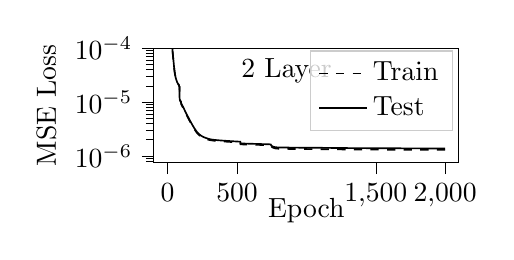
\begin{tikzpicture}

\begin{axis}[
legend cell align={left},
legend style={fill opacity=0.8, draw opacity=1, text opacity=1, draw=white!80!black},
log basis y={10},
tick align=outside,
tick pos=left,
title={2 Layer $\hy$},
title style={at={(0.45,0.85)},anchor=north},
x grid style={white!69.0196078431373!black},
xlabel={Epoch},
x label style={yshift=10pt},
xmin=-99.95, xmax=2098.95,
xtick style={color=black},
xtick = {0,500,1500,2000},
y grid style={white!69.0196078431373!black},
ylabel={MSE Loss},
ymin=7.6063321892292e-07, ymax=1e-4,
ymode=log,
ytick style={color=black},
width=.45\textwidth,
height=.25\textwidth
]
\addplot [semithick, black, dashed]
table {%
0 0.0518386695683002
1 0.042526340380311
2 0.0347423156872392
3 0.0278063397407532
4 0.021599099136889
5 0.0169535573758185
6 0.0133449736572802
7 0.0096524867080152
8 0.00607697855122387
9 0.00346671832166612
10 0.00228777943272144
11 0.00164228947134689
12 0.00122930787573569
13 0.000946592513937503
14 0.000754222130053677
15 0.000623254176578484
16 0.000526171202189289
17 0.000440977271879092
18 0.00037380238971673
19 0.000321372847538441
20 0.00028025879181223
21 0.000247563553391956
22 0.000221549878042424
23 0.000200674695734051
24 0.000183563173413859
25 0.000169053649296984
26 0.000156700562307378
27 0.000145990131146391
28 0.000136467741052911
29 0.000127828117649187
30 0.000119895841526159
31 0.000112545413488988
32 0.000105680738532101
33 9.92588357621571e-05
34 9.3258946260903e-05
35 8.76442736916943e-05
36 8.23576925613452e-05
37 7.73938517377246e-05
38 7.27130913655856e-05
39 6.8314350421133e-05
40 6.41955712490017e-05
41 6.03399962346884e-05
42 5.67417087368085e-05
43 5.33954841157538e-05
44 5.0292471962166e-05
45 4.74299892848649e-05
46 4.48063469739282e-05
47 4.24147469020681e-05
48 4.02486506536661e-05
49 3.82998454442713e-05
50 3.65582336962689e-05
51 3.50118609967467e-05
52 3.36569491373666e-05
53 3.24788894431549e-05
54 3.14478582076845e-05
55 3.05533147147798e-05
56 2.97498192085186e-05
57 2.89429238437151e-05
58 2.82225572700554e-05
59 2.75767276507395e-05
60 2.69969247092376e-05
61 2.646950968483e-05
62 2.59851477894699e-05
63 2.55374307816965e-05
64 2.51249913926586e-05
65 2.47355156570848e-05
66 2.43629243705072e-05
67 2.39832626575662e-05
68 2.35637702317035e-05
69 2.32211665752402e-05
70 2.29383413134201e-05
71 2.26900584239047e-05
72 2.24617844360182e-05
73 2.22450978726556e-05
74 2.20345916350197e-05
75 2.18275812112552e-05
76 2.16219654867018e-05
77 2.1417711785034e-05
78 2.1214236781816e-05
79 2.10117783281021e-05
80 2.08105283381883e-05
81 2.06107105623232e-05
82 2.04136253305478e-05
83 1.99121589284914e-05
84 1.94468321642489e-05
85 1.92526021455706e-05
86 1.68429254481453e-05
87 1.11265583582281e-05
88 1.08224221194178e-05
89 1.06731547539312e-05
90 1.05443111642671e-05
91 1.04219903960256e-05
92 1.03025638554755e-05
93 1.01851757890472e-05
94 1.00690036970263e-05
95 9.95377955223375e-06
96 9.83960515168292e-06
97 9.6077903663172e-06
98 9.08970189311731e-06
99 8.98518852409325e-06
100 8.88667989238456e-06
101 8.78861929595587e-06
102 8.69103235254443e-06
103 8.59354773410814e-06
104 8.49647685981836e-06
105 8.39990374788613e-06
106 8.30380843763123e-06
107 8.20817358044224e-06
108 8.11326919119892e-06
109 8.0190826447506e-06
110 7.92535356458757e-06
111 7.83217436401173e-06
112 7.73989984918444e-06
113 7.64807627137998e-06
114 7.5570470621642e-06
115 7.46617350023371e-06
116 7.37646823699834e-06
117 7.28749768268244e-06
118 7.19915332319943e-06
119 7.11171480043049e-06
120 7.0252807649922e-06
121 6.93957605744799e-06
122 6.8550750625036e-06
123 6.77161231669743e-06
124 6.68928749064435e-06
125 6.60800705782094e-06
126 6.52786106229541e-06
127 6.44881835250999e-06
128 6.3709648547956e-06
129 6.29415914409037e-06
130 6.21850223342335e-06
131 6.14401825305322e-06
132 6.07067480086698e-06
133 5.99841532675782e-06
134 5.92726610238969e-06
135 5.85724698703416e-06
136 5.78829684695847e-06
137 5.72039379244416e-06
138 5.65365198121981e-06
139 5.58796158020414e-06
140 5.52333012819872e-06
141 5.45967585458129e-06
142 5.39706647441562e-06
143 5.33535780868988e-06
144 5.27458272108561e-06
145 5.21480528050233e-06
146 5.15576177031107e-06
147 5.09760672775883e-06
148 5.04035929361635e-06
149 4.98399535490535e-06
150 4.92840583774523e-06
151 4.87364144305502e-06
152 4.81966467486927e-06
153 4.76406977395527e-06
154 4.69791715545398e-06
155 4.64507658807634e-06
156 4.59343973466275e-06
157 4.54271117132521e-06
158 4.49279561598814e-06
159 4.4436497382776e-06
160 4.39516718938648e-06
161 4.34741592334831e-06
162 4.30033761358573e-06
163 4.25400164704115e-06
164 4.20822800037968e-06
165 4.16278015359239e-06
166 4.1181904248333e-06
167 4.07423587330413e-06
168 4.0309002961294e-06
169 3.98809872649508e-06
170 3.94593327928305e-06
171 3.90432318772582e-06
172 3.86316539697873e-06
173 3.82265143798577e-06
174 3.78271101931205e-06
175 3.74335995593356e-06
176 3.70451060553023e-06
177 3.66598950404295e-06
178 3.62826339983258e-06
179 3.59102522270405e-06
180 3.55434255129694e-06
181 3.51821511981143e-06
182 3.4826161552246e-06
183 3.44756884828712e-06
184 3.41307895928367e-06
185 3.3791370713061e-06
186 3.34570067798268e-06
187 3.31284759954542e-06
188 3.28047421021438e-06
189 3.24868683401291e-06
190 3.21743388849427e-06
191 3.1866992187588e-06
192 3.15648334390062e-06
193 3.12686154870789e-06
194 3.09775542154966e-06
195 3.0692054060637e-06
196 3.04119435577377e-06
197 3.01375761148392e-06
198 2.98678445994938e-06
199 2.96039846932672e-06
200 2.93452443952447e-06
201 2.90920865177213e-06
202 2.88442320947979e-06
203 2.86015471203882e-06
204 2.83649073071501e-06
205 2.81332962913439e-06
206 2.79064786889194e-06
207 2.76854250500946e-06
208 2.74696784845219e-06
209 2.72586062430946e-06
210 2.70531269256935e-06
211 2.68526590684814e-06
212 2.66566363393395e-06
213 2.64662573533769e-06
214 2.6280339858431e-06
215 2.60993901497386e-06
216 2.59233656379365e-06
217 2.57519019442043e-06
218 2.55849347206549e-06
219 2.54225137109643e-06
220 2.52648555715496e-06
221 2.51116403057949e-06
222 2.49626635525146e-06
223 2.48174041792026e-06
224 2.46764998712479e-06
225 2.45395659851511e-06
226 2.44061466628409e-06
227 2.42766318024223e-06
228 2.41510581383864e-06
229 2.40287865153732e-06
230 2.39102976365757e-06
231 2.37946973879843e-06
232 2.36823859097512e-06
233 2.35734377997687e-06
234 2.34669803728593e-06
235 2.33637789938257e-06
236 2.32633338055166e-06
237 2.31655079858228e-06
238 2.30704811121996e-06
239 2.29775435502688e-06
240 2.28908307065012e-06
241 2.28025623937356e-06
242 2.27162592034347e-06
243 2.26319784212592e-06
244 2.2550409375981e-06
245 2.24706835138022e-06
246 2.23929092283015e-06
247 2.23166111379669e-06
248 2.22424669038901e-06
249 2.21699714541046e-06
250 2.20993513937628e-06
251 2.20302234424707e-06
252 2.19623759960541e-06
253 2.18960344636798e-06
254 2.18315790721135e-06
255 2.17678003446053e-06
256 2.17060044519712e-06
257 2.16451002290796e-06
258 2.15849525591238e-06
259 2.15263430231971e-06
260 2.14691730741379e-06
261 2.14129940786734e-06
262 2.13577006115884e-06
263 2.13036238608311e-06
264 2.12501493570016e-06
265 2.1199581875635e-06
266 2.11479780750778e-06
267 2.10963459062441e-06
268 2.10465096063217e-06
269 2.09979531643967e-06
270 2.09493869374455e-06
271 2.09029867505706e-06
272 2.08560229043542e-06
273 2.08097659026407e-06
274 2.07650576862761e-06
275 2.07193567734976e-06
276 2.06749240817317e-06
277 2.06326575550975e-06
278 2.05894802388684e-06
279 2.05470462492485e-06
280 2.05050052682054e-06
281 2.04643580877928e-06
282 2.0424704373454e-06
283 2.03852960294171e-06
284 2.03469342307017e-06
285 2.03091579976444e-06
286 2.02713633768781e-06
287 2.02345604839138e-06
288 2.01982171290638e-06
289 2.01625873410194e-06
290 2.01274700611975e-06
291 2.00929016750706e-06
292 2.00590146562263e-06
293 2.00254602100358e-06
294 1.99926750190116e-06
295 1.99598840447379e-06
296 1.99279543198827e-06
297 1.98967802123207e-06
298 1.98662693992446e-06
299 1.98363486015296e-06
300 1.98073774367913e-06
301 1.97792627022864e-06
302 1.97517233220879e-06
303 1.97249674567956e-06
304 1.96989209428011e-06
305 1.96735570136752e-06
306 1.96489110953735e-06
307 1.96252498756166e-06
308 1.96016407414845e-06
309 1.95790429916087e-06
310 1.95567747516634e-06
311 1.95353562503442e-06
312 1.95143923531305e-06
313 1.94938852894211e-06
314 1.94739756454965e-06
315 1.94547211549434e-06
316 1.94368945972201e-06
317 1.94186115868433e-06
318 1.94003258525299e-06
319 1.93824945745291e-06
320 1.9365728117009e-06
321 1.93486980356283e-06
322 1.93323022483582e-06
323 1.93159868342718e-06
324 1.93004855782419e-06
325 1.92850577320769e-06
326 1.92703124560012e-06
327 1.92557061188836e-06
328 1.92414228069993e-06
329 1.92272855258579e-06
330 1.92145235405405e-06
331 1.92011111062129e-06
332 1.91873049038804e-06
333 1.91744816731898e-06
334 1.91613417905501e-06
335 1.91486396772689e-06
336 1.91374089342844e-06
337 1.91252254262508e-06
338 1.91134569661244e-06
339 1.91014032100156e-06
340 1.90892861962766e-06
341 1.90778080786913e-06
342 1.90679503680258e-06
343 1.90562279988171e-06
344 1.90453983475436e-06
345 1.9034283604924e-06
346 1.90236943444688e-06
347 1.90128401038692e-06
348 1.90023423112962e-06
349 1.89921649234748e-06
350 1.89817762452549e-06
351 1.89717194177774e-06
352 1.89619797345131e-06
353 1.89519621744694e-06
354 1.89419035530136e-06
355 1.89321117386498e-06
356 1.89228158308197e-06
357 1.89132848026929e-06
358 1.89040515931538e-06
359 1.8894536552807e-06
360 1.88852625899472e-06
361 1.8876163518371e-06
362 1.88671577905097e-06
363 1.88581250529296e-06
364 1.88489490290067e-06
365 1.88400545243894e-06
366 1.88320691779609e-06
367 1.88227364219529e-06
368 1.88137783914044e-06
369 1.88048757183878e-06
370 1.87960764208128e-06
371 1.87875062977128e-06
372 1.87785555567643e-06
373 1.87700367860089e-06
374 1.8761265273497e-06
375 1.87530233984035e-06
376 1.87443296317724e-06
377 1.87359234882933e-06
378 1.87277639042804e-06
379 1.87191020336286e-06
380 1.87106933947234e-06
381 1.87022027148487e-06
382 1.86942492166509e-06
383 1.86859680513862e-06
384 1.86778859585957e-06
385 1.86696180901436e-06
386 1.86615413451818e-06
387 1.865346644081e-06
388 1.86454020524707e-06
389 1.86374061308925e-06
390 1.86296425601995e-06
391 1.86214191205636e-06
392 1.86135847434343e-06
393 1.86057959820118e-06
394 1.85977571720741e-06
395 1.85900325470811e-06
396 1.85821711534118e-06
397 1.85742586654669e-06
398 1.85668396852634e-06
399 1.85587053044856e-06
400 1.85511533595673e-06
401 1.85435227967901e-06
402 1.85357387726981e-06
403 1.85281492088052e-06
404 1.85205200068594e-06
405 1.85128828331926e-06
406 1.85053131349377e-06
407 1.8499851529441e-06
408 1.84917399599271e-06
409 1.84840255906238e-06
410 1.84766332199615e-06
411 1.84689625007195e-06
412 1.84613141198042e-06
413 1.84538050450556e-06
414 1.844629050197e-06
415 1.84387742933723e-06
416 1.84314657485629e-06
417 1.84239931502361e-06
418 1.84165844211748e-06
419 1.84091300036471e-06
420 1.84018742834269e-06
421 1.83944933723978e-06
422 1.83872336367585e-06
423 1.83799873639146e-06
424 1.83724605551561e-06
425 1.83653046701693e-06
426 1.83579679980994e-06
427 1.83508214388439e-06
428 1.83435587473468e-06
429 1.83363736755382e-06
430 1.8329269255446e-06
431 1.83219673760959e-06
432 1.83147712380105e-06
433 1.83076220457679e-06
434 1.83004805330711e-06
435 1.82932657037327e-06
436 1.82861742405294e-06
437 1.82790977305558e-06
438 1.82720573548067e-06
439 1.82647991425711e-06
440 1.82577657187721e-06
441 1.82505562622737e-06
442 1.82437355033471e-06
443 1.82366404123968e-06
444 1.82293964576274e-06
445 1.82224642969686e-06
446 1.82155447021159e-06
447 1.82083569222868e-06
448 1.82014943925424e-06
449 1.81945615088352e-06
450 1.81874204338328e-06
451 1.81806114380834e-06
452 1.8173547899778e-06
453 1.81667541403385e-06
454 1.81598416770612e-06
455 1.81524100480601e-06
456 1.81453961306488e-06
457 1.81385451594451e-06
458 1.81315790109693e-06
459 1.81245884846248e-06
460 1.81177978004143e-06
461 1.81107571381744e-06
462 1.81042428357614e-06
463 1.80971381985273e-06
464 1.80901504791109e-06
465 1.80835478647623e-06
466 1.80766282676359e-06
467 1.80698605220186e-06
468 1.80630960915096e-06
469 1.80562094067227e-06
470 1.80495204324416e-06
471 1.80429276622363e-06
472 1.80363471463352e-06
473 1.80292723803177e-06
474 1.80225790609256e-06
475 1.80158976775147e-06
476 1.80091279730732e-06
477 1.80023987002187e-06
478 1.79959257354767e-06
479 1.79890977392461e-06
480 1.79824207714319e-06
481 1.79757481157594e-06
482 1.7969080555531e-06
483 1.79623438566523e-06
484 1.79557559511068e-06
485 1.79491270898779e-06
486 1.79438170130197e-06
487 1.79366591225971e-06
488 1.79298442958498e-06
489 1.79231373408584e-06
490 1.79167655073798e-06
491 1.79100179059333e-06
492 1.79032596940942e-06
493 1.78968522516243e-06
494 1.78901104857232e-06
495 1.78837366763673e-06
496 1.78771149103341e-06
497 1.78705672965407e-06
498 1.78641258935386e-06
499 1.78577213569042e-06
500 1.78510025034484e-06
501 1.78445535595984e-06
502 1.78384143919175e-06
503 1.78316099584208e-06
504 1.7825342940796e-06
505 1.78187944834463e-06
506 1.78124007402403e-06
507 1.78060222037857e-06
508 1.77995303192802e-06
509 1.77932496455924e-06
510 1.77868458877128e-06
511 1.77803215694894e-06
512 1.77739755554285e-06
513 1.77675821737466e-06
514 1.77612358766055e-06
515 1.77547155703905e-06
516 1.77483872244011e-06
517 1.77422070601096e-06
518 1.7735807008421e-06
519 1.77294365573744e-06
520 1.77230281133234e-06
521 1.77169832647905e-06
522 1.77105510329056e-06
523 1.77042892869395e-06
524 1.76978312288156e-06
525 1.66620164694109e-06
526 1.63933637233526e-06
527 1.63880179010789e-06
528 1.63844974755989e-06
529 1.63812484262849e-06
530 1.63779529955832e-06
531 1.63742095688235e-06
532 1.63711894725793e-06
533 1.63679492797542e-06
534 1.63647552042789e-06
535 1.6361367341915e-06
536 1.63582143278518e-06
537 1.63551573919563e-06
538 1.63520860402855e-06
539 1.63490383059184e-06
540 1.63459672538124e-06
541 1.63429267476545e-06
542 1.63399191654889e-06
543 1.63368553430132e-06
544 1.63338495767107e-06
545 1.63310262541927e-06
546 1.6327682387498e-06
547 1.63247037161796e-06
548 1.63218582176228e-06
549 1.63187798207787e-06
550 1.6315871942254e-06
551 1.63128337254648e-06
552 1.63099369069641e-06
553 1.63070029680057e-06
554 1.63040730399189e-06
555 1.63011679620695e-06
556 1.62983160720387e-06
557 1.62952682003947e-06
558 1.62922214192918e-06
559 1.62894504913425e-06
560 1.62864188482104e-06
561 1.6283534936008e-06
562 1.6280654233185e-06
563 1.62778253840656e-06
564 1.62747459560819e-06
565 1.62719646951359e-06
566 1.62692239271678e-06
567 1.62661389299501e-06
568 1.62633292706005e-06
569 1.62606319807423e-06
570 1.62576276485993e-06
571 1.62547591571638e-06
572 1.62518481394613e-06
573 1.62490155244654e-06
574 1.62461253736979e-06
575 1.62433828410258e-06
576 1.62405268940802e-06
577 1.62376205736336e-06
578 1.62348133056867e-06
579 1.62319527444765e-06
580 1.62290394715114e-06
581 1.62262100627686e-06
582 1.62234837728192e-06
583 1.62206169241585e-06
584 1.6217815277173e-06
585 1.62149699008296e-06
586 1.62121524058989e-06
587 1.62092517706469e-06
588 1.62070420867622e-06
589 1.62038921615704e-06
590 1.62008199799857e-06
591 1.61979725899641e-06
592 1.61950673955857e-06
593 1.61922272562265e-06
594 1.6189295055824e-06
595 1.61864341677642e-06
596 1.61835239086372e-06
597 1.61807546018622e-06
598 1.61779094619874e-06
599 1.61749259794419e-06
600 1.61723098355537e-06
601 1.61693797414841e-06
602 1.61665728629146e-06
603 1.61636831695944e-06
604 1.61610073524798e-06
605 1.61582153997131e-06
606 1.61554774945216e-06
607 1.61525743881441e-06
608 1.61498842523145e-06
609 1.61470044996292e-06
610 1.61442914523491e-06
611 1.61414135411064e-06
612 1.61386748200698e-06
613 1.61359336857458e-06
614 1.61332622727173e-06
615 1.61304242104166e-06
616 1.61276320352499e-06
617 1.61248982448114e-06
618 1.61219475916141e-06
619 1.61193266151827e-06
620 1.61164703547456e-06
621 1.61138146705753e-06
622 1.61109890345301e-06
623 1.61082260021317e-06
624 1.61053988405513e-06
625 1.61026904530104e-06
626 1.6099991666465e-06
627 1.60971038680202e-06
628 1.60944881005776e-06
629 1.60917611752609e-06
630 1.60890855008233e-06
631 1.60862766114178e-06
632 1.60834999020665e-06
633 1.60807368021665e-06
634 1.60779430278524e-06
635 1.60753966724769e-06
636 1.60726439040104e-06
637 1.60700710711126e-06
638 1.60672452217625e-06
639 1.60644054170689e-06
640 1.60616960967275e-06
641 1.60589141702872e-06
642 1.60563484433851e-06
643 1.6053435355019e-06
644 1.60508566412432e-06
645 1.60482664446704e-06
646 1.60453707941599e-06
647 1.6042754193677e-06
648 1.60399306275849e-06
649 1.60374430119248e-06
650 1.6034647498202e-06
651 1.60318650912927e-06
652 1.60291618941244e-06
653 1.60264964672763e-06
654 1.60237670334595e-06
655 1.60212423365635e-06
656 1.60184172608524e-06
657 1.60158811885935e-06
658 1.60129746804216e-06
659 1.60103951819224e-06
660 1.60076912700902e-06
661 1.60050588327465e-06
662 1.60023428719569e-06
663 1.59996088962089e-06
664 1.59969389768833e-06
665 1.59941708385247e-06
666 1.59916993624165e-06
667 1.59889477750141e-06
668 1.59866888432703e-06
669 1.59837924398687e-06
670 1.59808459493149e-06
671 1.59782723729052e-06
672 1.5975413056708e-06
673 1.59727512193797e-06
674 1.59698751379267e-06
675 1.59672256081933e-06
676 1.59644536088877e-06
677 1.59617859861783e-06
678 1.59590370850538e-06
679 1.59562858524964e-06
680 1.59536997378495e-06
681 1.59507531752467e-06
682 1.59482622048301e-06
683 1.59457645222005e-06
684 1.59428069426326e-06
685 1.5940048189691e-06
686 1.59374665537371e-06
687 1.59347681504585e-06
688 1.59320771297189e-06
689 1.59294189681702e-06
690 1.59265840376577e-06
691 1.59240391452897e-06
692 1.59212388167873e-06
693 1.59185475271784e-06
694 1.59160081452114e-06
695 1.5913355798034e-06
696 1.59105049479535e-06
697 1.59078170094062e-06
698 1.5905177025104e-06
699 1.59024808239394e-06
700 1.5899925537326e-06
701 1.58970312894269e-06
702 1.58944773028225e-06
703 1.58917952906279e-06
704 1.58889819385877e-06
705 1.5886472953639e-06
706 1.58836964335762e-06
707 1.58811646971913e-06
708 1.58783535489704e-06
709 1.58757957046873e-06
710 1.58731703973558e-06
711 1.58704471705562e-06
712 1.58677873791646e-06
713 1.5865028876334e-06
714 1.58624447136901e-06
715 1.58597577814135e-06
716 1.58570803385771e-06
717 1.58545115763786e-06
718 1.58517122966373e-06
719 1.58490910264675e-06
720 1.58464107597922e-06
721 1.58438146414142e-06
722 1.58410357899186e-06
723 1.58384261210642e-06
724 1.58350118182682e-06
725 1.58321730540933e-06
726 1.58293486397554e-06
727 1.58265849421468e-06
728 1.58239726721376e-06
729 1.58211539564945e-06
730 1.58183252307253e-06
731 1.58156696035405e-06
732 1.58106459616647e-06
733 1.5807887297683e-06
734 1.580489066626e-06
735 1.58021400281427e-06
736 1.57994096404934e-06
737 1.57964867177895e-06
738 1.57935908634954e-06
739 1.57908623067726e-06
740 1.57895105029127e-06
741 1.57861684205329e-06
742 1.57829686450839e-06
743 1.57820503723372e-06
744 1.56886491616604e-06
745 1.54443650944813e-06
746 1.52464937485774e-06
747 1.5084941576049e-06
748 1.49567416087848e-06
749 1.48492991016269e-06
750 1.47589340608079e-06
751 1.46807804819105e-06
752 1.46103214052573e-06
753 1.45476694632407e-06
754 1.44896854914123e-06
755 1.44370241736169e-06
756 1.43866883598776e-06
757 1.43380883416455e-06
758 1.42928160187239e-06
759 1.42504067417804e-06
760 1.42097017825904e-06
761 1.41716485458687e-06
762 1.41355964707657e-06
763 1.41026495602148e-06
764 1.40694243066264e-06
765 1.40386480411792e-06
766 1.40090109704261e-06
767 1.39811546335977e-06
768 1.39556718215772e-06
769 1.39314711935867e-06
770 1.39085914671e-06
771 1.38873771130932e-06
772 1.38676904158785e-06
773 1.38486147091044e-06
774 1.38307318255215e-06
775 1.38140495923267e-06
776 1.37981144834498e-06
777 1.37832817009098e-06
778 1.37694258201293e-06
779 1.37560938435399e-06
780 1.3743737128209e-06
781 1.3732237981543e-06
782 1.3721374578779e-06
783 1.37116235606527e-06
784 1.37018989329363e-06
785 1.36925985286496e-06
786 1.36841710016711e-06
787 1.36757084865735e-06
788 1.36681302183206e-06
789 1.36608643293812e-06
790 1.36541132677337e-06
791 1.36474158155409e-06
792 1.36417904980135e-06
793 1.36355554245426e-06
794 1.36299955610752e-06
795 1.36246179810939e-06
796 1.36196002624445e-06
797 1.36147286586663e-06
798 1.36102072210065e-06
799 1.36058262586403e-06
800 1.36019539741028e-06
801 1.35977008343957e-06
802 1.35934900353618e-06
803 1.35907496527921e-06
804 1.35871082459005e-06
805 1.35838341267913e-06
806 1.35806158336038e-06
807 1.35770684502745e-06
808 1.35738369530713e-06
809 1.35709290060504e-06
810 1.35672559207478e-06
811 1.35645564012066e-06
812 1.35619012348798e-06
813 1.35594104767733e-06
814 1.35568918759077e-06
815 1.35547467380093e-06
816 1.35525254742674e-06
817 1.35503257631342e-06
818 1.35482675494814e-06
819 1.35461341591281e-06
820 1.35443167101812e-06
821 1.35425345231965e-06
822 1.3540686281317e-06
823 1.35388498344469e-06
824 1.35370961773162e-06
825 1.35353743995381e-06
826 1.3533792219107e-06
827 1.35313768534218e-06
828 1.35298258597061e-06
829 1.352827967807e-06
830 1.3526768412504e-06
831 1.35252841401723e-06
832 1.35240225704081e-06
833 1.35225109995929e-06
834 1.35212322014411e-06
835 1.35198998505359e-06
836 1.35184609810324e-06
837 1.35173012962753e-06
838 1.35159571098598e-06
839 1.35147283796755e-06
840 1.35134105134682e-06
841 1.35123280175264e-06
842 1.35110112422865e-06
843 1.35098620997098e-06
844 1.3508639218287e-06
845 1.35077587185606e-06
846 1.35064492155834e-06
847 1.35053679737496e-06
848 1.35042975225019e-06
849 1.35031924180851e-06
850 1.35021662519819e-06
851 1.35011604727708e-06
852 1.35000363111715e-06
853 1.34990536004409e-06
854 1.3498181129421e-06
855 1.34971324047228e-06
856 1.34960946446938e-06
857 1.34950742594242e-06
858 1.34941408889233e-06
859 1.34932775988261e-06
860 1.34922658703829e-06
861 1.34912472361748e-06
862 1.34902612357735e-06
863 1.34892750345728e-06
864 1.34883547387687e-06
865 1.34874449845768e-06
866 1.34864384494904e-06
867 1.34856915693149e-06
868 1.348471884981e-06
869 1.34839657053476e-06
870 1.34830537385255e-06
871 1.34821930835471e-06
872 1.34813692710622e-06
873 1.34803793085325e-06
874 1.34795173156022e-06
875 1.3478776119058e-06
876 1.34777355222582e-06
877 1.34769706210136e-06
878 1.34761042174603e-06
879 1.34751966670876e-06
880 1.34744346894422e-06
881 1.34735287390697e-06
882 1.34725689983384e-06
883 1.34717631696901e-06
884 1.34709783374376e-06
885 1.34702141804155e-06
886 1.34693583878231e-06
887 1.34685476582774e-06
888 1.34676708303516e-06
889 1.34668838386176e-06
890 1.3466111598035e-06
891 1.34654315939997e-06
892 1.34647579018576e-06
893 1.34638291420686e-06
894 1.34629611308412e-06
895 1.34621114347055e-06
896 1.34613849976972e-06
897 1.34607026022593e-06
898 1.34600097389637e-06
899 1.34590469681939e-06
900 1.34583183752568e-06
901 1.3457547924105e-06
902 1.34568102149046e-06
903 1.34570885896323e-06
904 1.34563602135529e-06
905 1.34554965568157e-06
906 1.34547586169731e-06
907 1.34539394407795e-06
908 1.34532783863506e-06
909 1.34524034038463e-06
910 1.34516967027309e-06
911 1.34509670238003e-06
912 1.34502306164563e-06
913 1.34495103804966e-06
914 1.34488076425043e-06
915 1.34479510651886e-06
916 1.34472651404849e-06
917 1.34466214339568e-06
918 1.34458127747905e-06
919 1.34450533219876e-06
920 1.3444267981555e-06
921 1.34435084679296e-06
922 1.34428695463384e-06
923 1.34422671932555e-06
924 1.34414231379765e-06
925 1.34407956909399e-06
926 1.3439992275579e-06
927 1.3439298076463e-06
928 1.34387832962091e-06
929 1.3438092536262e-06
930 1.34373289975542e-06
931 1.3436577213497e-06
932 1.34358143714053e-06
933 1.34352394559301e-06
934 1.34345717660267e-06
935 1.34337900578885e-06
936 1.34335605609692e-06
937 1.34328150070928e-06
938 1.34321433966988e-06
939 1.34313157009558e-06
940 1.3430716178533e-06
941 1.34299877356625e-06
942 1.3429399402014e-06
943 1.34285865880202e-06
944 1.34280206063409e-06
945 1.34274019325176e-06
946 1.34266461981269e-06
947 1.34259506944545e-06
948 1.34254850138404e-06
949 1.34247986547109e-06
950 1.34240087921e-06
951 1.34232612865048e-06
952 1.3423135030024e-06
953 1.34225830529999e-06
954 1.3421897558743e-06
955 1.34212832678315e-06
956 1.34206213189714e-06
957 1.34198343585012e-06
958 1.34193174501718e-06
959 1.34187326334256e-06
960 1.34180413468243e-06
961 1.34174007241938e-06
962 1.34166821864312e-06
963 1.34160912554648e-06
964 1.34154919388152e-06
965 1.34148838895953e-06
966 1.34141044561886e-06
967 1.34135855292072e-06
968 1.34130112543573e-06
969 1.34123174636613e-06
970 1.34118099316538e-06
971 1.34110277215882e-06
972 1.34103400789343e-06
973 1.34098474899247e-06
974 1.34092078039316e-06
975 1.34086393288158e-06
976 1.34079251927233e-06
977 1.34072488621939e-06
978 1.34067154296247e-06
979 1.34060519832246e-06
980 1.34055623038876e-06
981 1.34048152499133e-06
982 1.3404323760966e-06
983 1.34035964379109e-06
984 1.34030211174263e-06
985 1.34024774162356e-06
986 1.34017881156012e-06
987 1.3401354625131e-06
988 1.34007251983803e-06
989 1.34001645538717e-06
990 1.33994008200489e-06
991 1.33989448013949e-06
992 1.33979940444817e-06
993 1.3397541583231e-06
994 1.33968041419052e-06
995 1.33962406884791e-06
996 1.33956490974185e-06
997 1.33950567945362e-06
998 1.33946297422938e-06
999 1.33938883983831e-06
1000 1.33933092904215e-06
1001 1.33928694378937e-06
1002 1.33921256117731e-06
1003 1.33916161001935e-06
1004 1.3390988379598e-06
1005 1.33903752758613e-06
1006 1.33898176045477e-06
1007 1.33892504666733e-06
1008 1.33887592123472e-06
1009 1.33881134048863e-06
1010 1.33875219198387e-06
1011 1.33870028915339e-06
1012 1.33863348575858e-06
1013 1.33858250521257e-06
1014 1.33852591613959e-06
1015 1.33846663027271e-06
1016 1.33840421788989e-06
1017 1.33835072642796e-06
1018 1.33830789980038e-06
1019 1.33824401744675e-06
1020 1.33817713299322e-06
1021 1.33813398639404e-06
1022 1.33806409412784e-06
1023 1.33800658908001e-06
1024 1.33795149331206e-06
1025 1.3379155276283e-06
1026 1.33784969801809e-06
1027 1.33778447249711e-06
1028 1.33765031387156e-06
1029 1.33759461118643e-06
1030 1.33753808258064e-06
1031 1.33748855502347e-06
1032 1.33742270143955e-06
1033 1.33736784084704e-06
1034 1.33731045195873e-06
1035 1.33725952910879e-06
1036 1.33719250703734e-06
1037 1.33714265534479e-06
1038 1.33709573304941e-06
1039 1.33703461840184e-06
1040 1.33698563801943e-06
1041 1.33692117942985e-06
1042 1.33686207065864e-06
1043 1.33682150280379e-06
1044 1.33675993406257e-06
1045 1.33670628150639e-06
1046 1.33664372732767e-06
1047 1.33658942088744e-06
1048 1.33653863915129e-06
1049 1.33648365992656e-06
1050 1.33643210853052e-06
1051 1.33637117450292e-06
1052 1.33631502657749e-06
1053 1.33626177149893e-06
1054 1.33622257948218e-06
1055 1.33616662400016e-06
1056 1.33610955839458e-06
1057 1.33605329271802e-06
1058 1.33598385832556e-06
1059 1.33594217295752e-06
1060 1.33588493156367e-06
1061 1.33583359792055e-06
1062 1.33576979409611e-06
1063 1.33572435426288e-06
1064 1.33567137682178e-06
1065 1.33562173462565e-06
1066 1.33556964851778e-06
1067 1.33551589878778e-06
1068 1.33546273754348e-06
1069 1.33540153122169e-06
1070 1.33536268666035e-06
1071 1.33529603027682e-06
1072 1.33524601922375e-06
1073 1.33519661385151e-06
1074 1.33514066943974e-06
1075 1.33509146333211e-06
1076 1.33504329576795e-06
1077 1.33499757205868e-06
1078 1.33493545313001e-06
1079 1.33489117727947e-06
1080 1.33483645198851e-06
1081 1.33478451633096e-06
1082 1.33473267716511e-06
1083 1.33466724497566e-06
1084 1.33462421723607e-06
1085 1.33456596925896e-06
1086 1.33453018727892e-06
1087 1.33446277706639e-06
1088 1.33441716130278e-06
1089 1.33436078276361e-06
1090 1.33430692164893e-06
1091 1.33425975168677e-06
1092 1.33421545604051e-06
1093 1.33415072625098e-06
1094 1.33410108566068e-06
1095 1.33404680869376e-06
1096 1.33399491723196e-06
1097 1.33394408973686e-06
1098 1.33389038987275e-06
1099 1.33383919941821e-06
1100 1.33379414305068e-06
1101 1.33373261306247e-06
1102 1.33368463527006e-06
1103 1.33363207953607e-06
1104 1.33359130424537e-06
1105 1.33354491660498e-06
1106 1.33348266453481e-06
1107 1.33343180641532e-06
1108 1.33338205131395e-06
1109 1.33333231407562e-06
1110 1.33328824017553e-06
1111 1.33323012887843e-06
1112 1.33317537382993e-06
1113 1.33314741407276e-06
1114 1.33307755031353e-06
1115 1.33303352079395e-06
1116 1.33297956337231e-06
1117 1.3329289483579e-06
1118 1.33287542442417e-06
1119 1.33282477237628e-06
1120 1.33277926930475e-06
1121 1.33273204622242e-06
1122 1.33267181597319e-06
1123 1.332627589818e-06
1124 1.33257524055352e-06
1125 1.33252936851136e-06
1126 1.33248547196274e-06
1127 1.33243876933875e-06
1128 1.33238333026497e-06
1129 1.33232479907974e-06
1130 1.33227799227598e-06
1131 1.33223086616852e-06
1132 1.33218174798344e-06
1133 1.33213632797435e-06
1134 1.33208051036604e-06
1135 1.33205012393489e-06
1136 1.33198282409808e-06
1137 1.33193860241931e-06
1138 1.33188387665939e-06
1139 1.33183967609796e-06
1140 1.33179460509325e-06
1141 1.33174281238269e-06
1142 1.33169365426511e-06
1143 1.33164133212915e-06
1144 1.33158321374083e-06
1145 1.3315432472325e-06
1146 1.33148943393735e-06
1147 1.33144728846446e-06
1148 1.33139592961129e-06
1149 1.33134038986782e-06
1150 1.33129153603306e-06
1151 1.33124128893769e-06
1152 1.3311990425251e-06
1153 1.33114998108397e-06
1154 1.33109154313615e-06
1155 1.33104795212091e-06
1156 1.33099706505391e-06
1157 1.33095313810827e-06
1158 1.33090183919649e-06
1159 1.3308592359067e-06
1160 1.33080201646862e-06
1161 1.33075989552367e-06
1162 1.33070932677981e-06
1163 1.33065972174506e-06
1164 1.3306096723511e-06
1165 1.33056723711888e-06
1166 1.33051543905083e-06
1167 1.33045599883985e-06
1168 1.33043390209764e-06
1169 1.33039126671974e-06
1170 1.33034304828072e-06
1171 1.33029533026274e-06
1172 1.33023865356563e-06
1173 1.33019446022331e-06
1174 1.33014583248325e-06
1175 1.33009934955908e-06
1176 1.33004679793203e-06
1177 1.32999394267586e-06
1178 1.32859383582229e-06
1179 1.32577590167671e-06
1180 1.32481529779227e-06
1181 1.32425906130607e-06
1182 1.32385161771253e-06
1183 1.32355970555409e-06
1184 1.32332581735284e-06
1185 1.32313855300481e-06
1186 1.32299621942877e-06
1187 1.32287166445622e-06
1188 1.32275965106032e-06
1189 1.32266207796761e-06
1190 1.32258898742066e-06
1191 1.32251438074604e-06
1192 1.3224399087477e-06
1193 1.32236959144905e-06
1194 1.32232037235269e-06
1195 1.32225536714259e-06
1196 1.32219561778868e-06
1197 1.32214652194307e-06
1198 1.32208095470787e-06
1199 1.32204806527625e-06
1200 1.32199041914305e-06
1201 1.32194223348847e-06
1202 1.32188372917597e-06
1203 1.32185073353241e-06
1204 1.32179744296934e-06
1205 1.3217571945745e-06
1206 1.32170356749839e-06
1207 1.32168178934933e-06
1208 1.32160852400887e-06
1209 1.32156865880972e-06
1210 1.3215270177227e-06
1211 1.32148737561977e-06
1212 1.32144626445552e-06
1213 1.32139509810258e-06
1214 1.32141864840207e-06
1215 1.32135991154314e-06
1216 1.32131602497054e-06
1217 1.32127464453902e-06
1218 1.32121060731549e-06
1219 1.32116699967355e-06
1220 1.3211242721809e-06
1221 1.32107436284912e-06
1222 1.32103417314511e-06
1223 1.32099427466414e-06
1224 1.32095226790341e-06
1225 1.32089809829949e-06
1226 1.32086301134393e-06
1227 1.32081426257002e-06
1228 1.3207805423292e-06
1229 1.3207305637053e-06
1230 1.32068811232955e-06
1231 1.32064384796138e-06
1232 1.32060167554471e-06
1233 1.3205631688038e-06
1234 1.3205066439923e-06
1235 1.32047018907144e-06
1236 1.32054637529677e-06
1237 1.3205274783985e-06
1238 1.32047940205382e-06
1239 1.32043280677863e-06
1240 1.32039506168269e-06
1241 1.32036514655454e-06
1242 1.32031703172686e-06
1243 1.32027795616807e-06
1244 1.3202443684861e-06
1245 1.32019133667427e-06
1246 1.32015820261699e-06
1247 1.32011709712287e-06
1248 1.32007585411031e-06
1249 1.32003833635963e-06
1250 1.31999951743467e-06
1251 1.31995052718992e-06
1252 1.31991537205067e-06
1253 1.31987489763219e-06
1254 1.31983271600689e-06
1255 1.31978467074134e-06
1256 1.319753576837e-06
1257 1.31970657953673e-06
1258 1.31966508058667e-06
1259 1.319630016269e-06
1260 1.31958882650451e-06
1261 1.31953997157552e-06
1262 1.31951191637825e-06
1263 1.31946960593154e-06
1264 1.31942758504522e-06
1265 1.31938184219393e-06
1266 1.31933255261174e-06
1267 1.31929545118226e-06
1268 1.31925781937525e-06
1269 1.31922233245518e-06
1270 1.31924204031009e-06
1271 1.31918251739194e-06
1272 1.31914621874785e-06
1273 1.31909760800397e-06
1274 1.31904689864371e-06
1275 1.31899939506752e-06
1276 1.31895242788005e-06
1277 1.31888589362461e-06
1278 1.3188213102211e-06
1279 1.31876878970161e-06
1280 1.31870717576987e-06
1281 1.31865774105222e-06
1282 1.31860239366688e-06
1283 1.31855959794791e-06
1284 1.31852673801802e-06
1285 1.31848573423099e-06
1286 1.31843639238127e-06
1287 1.31837194871309e-06
1288 1.31832015325983e-06
1289 1.31827320812761e-06
1290 1.31821452710312e-06
1291 1.31826412868463e-06
1292 1.31820652498504e-06
1293 1.31813436787809e-06
1294 1.31808043758497e-06
1295 1.31803203781544e-06
1296 1.31797565646252e-06
1297 1.31792156848576e-06
1298 1.31787510680681e-06
1299 1.31782350318588e-06
1300 1.31777007236167e-06
1301 1.317731111385e-06
1302 1.31768447428726e-06
1303 1.31765222302249e-06
1304 1.31759061208925e-06
1305 1.3175407495396e-06
1306 1.31750282601217e-06
1307 1.31745717092713e-06
1308 1.31740909702671e-06
1309 1.31737010387667e-06
1310 1.31731581387839e-06
1311 1.31729359902977e-06
1312 1.31723423439212e-06
1313 1.31719637688832e-06
1314 1.31714781051073e-06
1315 1.31711109040111e-06
1316 1.31705777398849e-06
1317 1.31702496820196e-06
1318 1.31698145554537e-06
1319 1.31693504215491e-06
1320 1.316892996158e-06
1321 1.31685051350416e-06
1322 1.3168058811317e-06
1323 1.31676369285572e-06
1324 1.3167272482093e-06
1325 1.31667373887012e-06
1326 1.31663302317975e-06
1327 1.31659156795649e-06
1328 1.31655225268901e-06
1329 1.31651966761126e-06
1330 1.31647060948126e-06
1331 1.31643030140083e-06
1332 1.31639117168447e-06
1333 1.31633731963632e-06
1334 1.31630387018333e-06
1335 1.31626258671247e-06
1336 1.31621279176386e-06
1337 1.31617875889845e-06
1338 1.31613359954486e-06
1339 1.31608632344182e-06
1340 1.31604712120748e-06
1341 1.31601232321543e-06
1342 1.3159628022521e-06
1343 1.31592109164558e-06
1344 1.31588097301005e-06
1345 1.31584353617598e-06
1346 1.3158043823438e-06
1347 1.31577746958556e-06
1348 1.31573951045993e-06
1349 1.31568544951222e-06
1350 1.31564648904714e-06
1351 1.31560409097631e-06
1352 1.31556468213034e-06
1353 1.31551994411439e-06
1354 1.31547720894787e-06
1355 1.31544238529102e-06
1356 1.31539883138032e-06
1357 1.3153504088308e-06
1358 1.31530955987103e-06
1359 1.31526198380527e-06
1360 1.31523578205872e-06
1361 1.3151850012747e-06
1362 1.31514612101569e-06
1363 1.31510655799616e-06
1364 1.31506297603323e-06
1365 1.31502549686502e-06
1366 1.31497581915596e-06
1367 1.31494573567181e-06
1368 1.31489326294343e-06
1369 1.31486664048452e-06
1370 1.31481228511632e-06
1371 1.31477881735975e-06
1372 1.31473155177275e-06
1373 1.31468939930812e-06
1374 1.31464601584241e-06
1375 1.31461001865318e-06
1376 1.31457059183049e-06
1377 1.31452871148952e-06
1378 1.31448866785888e-06
1379 1.31444212428278e-06
1380 1.31440802965699e-06
1381 1.31436307299282e-06
1382 1.31431838971707e-06
1383 1.31427322443756e-06
1384 1.31423886649884e-06
1385 1.31420234399116e-06
1386 1.31415619608788e-06
1387 1.31413195184393e-06
1388 1.31408533862043e-06
1389 1.3140527643003e-06
1390 1.3140024599636e-06
1391 1.31395506453202e-06
1392 1.31391883945753e-06
1393 1.31387949465989e-06
1394 1.31384093273823e-06
1395 1.31380773196099e-06
1396 1.31375993719018e-06
1397 1.31372225746418e-06
1398 1.31367593549214e-06
1399 1.31363591665945e-06
1400 1.31359878579929e-06
1401 1.31356280685679e-06
1402 1.31351572737515e-06
1403 1.31348148261168e-06
1404 1.31343552995133e-06
1405 1.31340653955192e-06
1406 1.31335477141192e-06
1407 1.31331217909292e-06
1408 1.31328199159952e-06
1409 1.31324050759929e-06
1410 1.313199410518e-06
1411 1.31315960558709e-06
1412 1.31310952575348e-06
1413 1.31307809232339e-06
1414 1.31303962449181e-06
1415 1.3129952787807e-06
1416 1.31295043550494e-06
1417 1.31291564053981e-06
1418 1.31287857932705e-06
1419 1.31284263386533e-06
1420 1.31279429353981e-06
1421 1.31275722567636e-06
1422 1.31273118608988e-06
1423 1.31268142855845e-06
1424 1.3126316385268e-06
1425 1.31259607421441e-06
1426 1.31256069056462e-06
1427 1.31251248853914e-06
1428 1.31246915155714e-06
1429 1.31243717203233e-06
1430 1.31239350761803e-06
1431 1.31234716056383e-06
1432 1.3123242802493e-06
1433 1.31227735960238e-06
1434 1.31223271989711e-06
1435 1.31219915439829e-06
1436 1.31215062850742e-06
1437 1.31212218929022e-06
1438 1.3120791121537e-06
1439 1.31203161237181e-06
1440 1.31200182872249e-06
1441 1.31196549817503e-06
1442 1.31192107697586e-06
1443 1.31187962790591e-06
1444 1.31183938752599e-06
1445 1.31180776863005e-06
1446 1.31176054296134e-06
1447 1.31172362119969e-06
1448 1.31168643122237e-06
1449 1.31165350231299e-06
1450 1.31160334724711e-06
1451 1.3115657474998e-06
1452 1.311524503123e-06
1453 1.31148720245733e-06
1454 1.31145775291941e-06
1455 1.31141236701637e-06
1456 1.31137372878243e-06
1457 1.31133921740911e-06
1458 1.31128970619443e-06
1459 1.31125061385262e-06
1460 1.31120704479315e-06
1461 1.31118090965288e-06
1462 1.31113069129185e-06
1463 1.31109799757212e-06
1464 1.31105958655553e-06
1465 1.31102414700024e-06
1466 1.31113465407395e-06
1467 1.3115353781501e-06
1468 1.31073669899706e-06
1469 1.31061095918028e-06
1470 1.31053976475926e-06
1471 1.31051849380981e-06
1472 1.31045500958749e-06
1473 1.31041446591951e-06
1474 1.31038325683619e-06
1475 1.31034178316725e-06
1476 1.31030691308354e-06
1477 1.31025875219848e-06
1478 1.31020995374342e-06
1479 1.31017023034019e-06
1480 1.31014068551849e-06
1481 1.31009896698231e-06
1482 1.31005129526329e-06
1483 1.31001381359397e-06
1484 1.30997352819406e-06
1485 1.30993995983886e-06
1486 1.30989869869325e-06
1487 1.30986009870071e-06
1488 1.30982312171568e-06
1489 1.30978367678836e-06
1490 1.30974461123401e-06
1491 1.30970787867568e-06
1492 1.30966502571539e-06
1493 1.3096298849149e-06
1494 1.30959659510665e-06
1495 1.30956331126697e-06
1496 1.30951565556359e-06
1497 1.3094790621011e-06
1498 1.30944215527506e-06
1499 1.30939618007631e-06
1500 1.30936962753481e-06
1501 1.30933061875282e-06
1502 1.30928901221239e-06
1503 1.30924293445389e-06
1504 1.30921448861443e-06
1505 1.30917329974523e-06
1506 1.3091434063881e-06
1507 1.3091095128317e-06
1508 1.30906401409447e-06
1509 1.30902855379134e-06
1510 1.30899295051279e-06
1511 1.30895525619223e-06
1512 1.30891014282497e-06
1513 1.30888283999298e-06
1514 1.30883949670135e-06
1515 1.30880467609984e-06
1516 1.30876093874122e-06
1517 1.30873182040148e-06
1518 1.30869287713153e-06
1519 1.30865213854747e-06
1520 1.30861667719273e-06
1521 1.3085740121852e-06
1522 1.30854242374312e-06
1523 1.30850691304829e-06
1524 1.30846172521615e-06
1525 1.3084308924789e-06
1526 1.30839026867591e-06
1527 1.30835211136571e-06
1528 1.30831085695604e-06
1529 1.30828064069988e-06
1530 1.308229396912e-06
1531 1.3081966038726e-06
1532 1.30816021432167e-06
1533 1.30811588522306e-06
1534 1.30807387886023e-06
1535 1.30804364836479e-06
1536 1.30800523677976e-06
1537 1.3079673543217e-06
1538 1.30793483285174e-06
1539 1.30789522229691e-06
1540 1.30785042148318e-06
1541 1.30781459185414e-06
1542 1.30778182165159e-06
1543 1.30775194134003e-06
1544 1.30771855249634e-06
1545 1.30767076348093e-06
1546 1.30763190119865e-06
1547 1.30759709659856e-06
1548 1.30755398699023e-06
1549 1.30752424855984e-06
1550 1.30748375099188e-06
1551 1.30745104392815e-06
1552 1.30741234369225e-06
1553 1.30737575641149e-06
1554 1.30733214440681e-06
1555 1.30730984595573e-06
1556 1.3072714322675e-06
1557 1.30723216413742e-06
1558 1.30718758191506e-06
1559 1.307162111857e-06
1560 1.3071203532462e-06
1561 1.30709440516341e-06
1562 1.30705507541506e-06
1563 1.30701736974004e-06
1564 1.30697946784153e-06
1565 1.30694769262618e-06
1566 1.30688747393037e-06
1567 1.30680106401826e-06
1568 1.30671250040848e-06
1569 1.30658519580606e-06
1570 1.30647350641766e-06
1571 1.30637264372524e-06
1572 1.30628260801302e-06
1573 1.30619263643439e-06
1574 1.30612632679572e-06
1575 1.3060445271833e-06
1576 1.30598045691954e-06
1577 1.30592523802875e-06
1578 1.30587186585274e-06
1579 1.30581472285485e-06
1580 1.30576124846016e-06
1581 1.30571444087479e-06
1582 1.30566849995262e-06
1583 1.30562871432005e-06
1584 1.30558825976834e-06
1585 1.30554417266637e-06
1586 1.30550023445153e-06
1587 1.30546279150678e-06
1588 1.30542278432699e-06
1589 1.30538380547307e-06
1590 1.30534058511955e-06
1591 1.30530249140293e-06
1592 1.30526528718633e-06
1593 1.30523094507851e-06
1594 1.30519310198451e-06
1595 1.30515999937586e-06
1596 1.30511330560523e-06
1597 1.30507664401591e-06
1598 1.30503874788701e-06
1599 1.30500457611049e-06
1600 1.30496916459322e-06
1601 1.30494285006932e-06
1602 1.30490435564923e-06
1603 1.30485838994332e-06
1604 1.30482659885445e-06
1605 1.30478732155837e-06
1606 1.3047524880534e-06
1607 1.30471406019694e-06
1608 1.30468427630603e-06
1609 1.30464755363846e-06
1610 1.30461211692534e-06
1611 1.30457956852581e-06
1612 1.3045466137811e-06
1613 1.30451384271169e-06
1614 1.30447131995481e-06
1615 1.30443236731992e-06
1616 1.30440879334515e-06
1617 1.30436869623907e-06
1618 1.30434016888614e-06
1619 1.30430917424462e-06
1620 1.30427162395108e-06
1621 1.30423100985411e-06
1622 1.30420232578388e-06
1623 1.30416617172102e-06
1624 1.3041299450407e-06
1625 1.30410262495673e-06
1626 1.30406100817027e-06
1627 1.30401921336443e-06
1628 1.30399914212376e-06
1629 1.30395539915185e-06
1630 1.30392317404926e-06
1631 1.30389736538916e-06
1632 1.30385062966809e-06
1633 1.30381534091839e-06
1634 1.30380177922973e-06
1635 1.30375087475443e-06
1636 1.30372180177574e-06
1637 1.3036884428459e-06
1638 1.30364403828764e-06
1639 1.30360659640871e-06
1640 1.30358346132198e-06
1641 1.30354482784867e-06
1642 1.30351669014317e-06
1643 1.30347193973535e-06
1644 1.30343639024488e-06
1645 1.30340346458979e-06
1646 1.30337845570239e-06
1647 1.30333353850176e-06
1648 1.30331501819114e-06
1649 1.30327775123362e-06
1650 1.30324178195451e-06
1651 1.30319812065238e-06
1652 1.30316767285876e-06
1653 1.30314653416974e-06
1654 1.30310440718517e-06
1655 1.30306319319118e-06
1656 1.30303104739937e-06
1657 1.3029972061247e-06
1658 1.30295640188649e-06
1659 1.30292751202887e-06
1660 1.30288585020821e-06
1661 1.3028596930269e-06
1662 1.30282386928116e-06
1663 1.30279087981933e-06
1664 1.30276015883624e-06
1665 1.30272269737475e-06
1666 1.30268822775292e-06
1667 1.30265419538489e-06
1668 1.30262256087121e-06
1669 1.30258766282054e-06
1670 1.30255358023135e-06
1671 1.30251958941585e-06
1672 1.3024827413517e-06
1673 1.30244834473103e-06
1674 1.30242112800261e-06
1675 1.30238559525253e-06
1676 1.30235082198737e-06
1677 1.30231930461377e-06
1678 1.30228147989442e-06
1679 1.30225140925688e-06
1680 1.30221264949171e-06
1681 1.3021771924997e-06
1682 1.30215629911845e-06
1683 1.30212054297374e-06
1684 1.3020825262231e-06
1685 1.30205074025014e-06
1686 1.30201645512784e-06
1687 1.3019760089179e-06
1688 1.30194387260474e-06
1689 1.30191285383319e-06
1690 1.30188629354677e-06
1691 1.30184348482487e-06
1692 1.30181177200939e-06
1693 1.30178400208081e-06
1694 1.3017502183601e-06
1695 1.30171701061954e-06
1696 1.30168398564479e-06
1697 1.30165680079131e-06
1698 1.30161776992566e-06
1699 1.30158671188951e-06
1700 1.301542995094e-06
1701 1.30151153366853e-06
1702 1.30147992234697e-06
1703 1.30145104238011e-06
1704 1.30140742756169e-06
1705 1.30138871969621e-06
1706 1.30135159645306e-06
1707 1.30132069060096e-06
1708 1.30128667251483e-06
1709 1.30124737745518e-06
1710 1.30121323856258e-06
1711 1.30118363685483e-06
1712 1.30115531682407e-06
1713 1.30111670598865e-06
1714 1.30109344169682e-06
1715 1.30105685009596e-06
1716 1.3010196516916e-06
1717 1.30099644994175e-06
1718 1.30095129730989e-06
1719 1.30092531632897e-06
1720 1.30088796163363e-06
1721 1.3008512727879e-06
1722 1.30082383361696e-06
1723 1.30078734325423e-06
1724 1.30075498084636e-06
1725 1.30072494835076e-06
1726 1.30069480792372e-06
1727 1.30066290452646e-06
1728 1.30062102641659e-06
1729 1.30059479585043e-06
1730 1.30056997774375e-06
1731 1.30052966622429e-06
1732 1.30049582769232e-06
1733 1.30045942457002e-06
1734 1.30042508709494e-06
1735 1.30040336006232e-06
1736 1.30036208952333e-06
1737 1.30033579117139e-06
1738 1.30031166487754e-06
1739 1.30027404554767e-06
1740 1.30023207418617e-06
1741 1.30020137497411e-06
1742 1.30016529365662e-06
1743 1.30013674007046e-06
1744 1.3001077397945e-06
1745 1.30007461308423e-06
1746 1.30003726891914e-06
1747 1.30001273335267e-06
1748 1.29998552732502e-06
1749 1.29994284267809e-06
1750 1.29990960890325e-06
1751 1.29988650238033e-06
1752 1.29984577939979e-06
1753 1.29981313244798e-06
1754 1.29978438639e-06
1755 1.29974981085468e-06
1756 1.29972055978556e-06
1757 1.29969358975757e-06
1758 1.29965266478393e-06
1759 1.29962256363569e-06
1760 1.29958961294108e-06
1761 1.29955889558175e-06
1762 1.29952550526014e-06
1763 1.29949171279975e-06
1764 1.29945958289568e-06
1765 1.29943046847814e-06
1766 1.29939997185602e-06
1767 1.29936943054076e-06
1768 1.29933621389e-06
1769 1.29929934533379e-06
1770 1.29926757435328e-06
1771 1.2992392044282e-06
1772 1.29920533100858e-06
1773 1.2991700671563e-06
1774 1.29912627332374e-06
1775 1.29909210278356e-06
1776 1.29906255446599e-06
1777 1.29903083757199e-06
1778 1.29900498477298e-06
1779 1.29897524021771e-06
1780 1.29893359738276e-06
1781 1.29891209623167e-06
1782 1.29887807187856e-06
1783 1.29884300372396e-06
1784 1.2988116064605e-06
1785 1.29877996954519e-06
1786 1.29874484923675e-06
1787 1.2987117428338e-06
1788 1.29867583009968e-06
1789 1.29864896672416e-06
1790 1.29861854901492e-06
1791 1.29858806143091e-06
1792 1.29855296736991e-06
1793 1.29853388322942e-06
1794 1.29849827672501e-06
1795 1.29846098039366e-06
1796 1.29843629670745e-06
1797 1.29840156135685e-06
1798 1.29837512514541e-06
1799 1.29836212408918e-06
1800 1.29831896404653e-06
1801 1.29829055092046e-06
1802 1.2982576319871e-06
1803 1.29823140947849e-06
1804 1.29820048537965e-06
1805 1.29817173797164e-06
1806 1.29814512463611e-06
1807 1.2981023378984e-06
1808 1.29807500867685e-06
1809 1.29803826821728e-06
1810 1.29800773646593e-06
1811 1.2979781847946e-06
1812 1.29794077389533e-06
1813 1.29791346279262e-06
1814 1.29788016687371e-06
1815 1.29784268041533e-06
1816 1.29782022439429e-06
1817 1.29778623839627e-06
1818 1.2977592077732e-06
1819 1.29772728793398e-06
1820 1.29769857242934e-06
1821 1.29766320105773e-06
1822 1.29762787879883e-06
1823 1.29760096830012e-06
1824 1.2975656488976e-06
1825 1.29753746644212e-06
1826 1.2975013315355e-06
1827 1.29748086591519e-06
1828 1.2974416726621e-06
1829 1.29741440080977e-06
1830 1.29738914618827e-06
1831 1.29735291490363e-06
1832 1.29731755794182e-06
1833 1.297284848917e-06
1834 1.29725806272063e-06
1835 1.29722429477397e-06
1836 1.29719462270828e-06
1837 1.29716277369596e-06
1838 1.297132099495e-06
1839 1.29710682350037e-06
1840 1.29707580282457e-06
1841 1.29704243165918e-06
1842 1.29701305678509e-06
1843 1.29698461583416e-06
1844 1.29694613946185e-06
1845 1.2969152633957e-06
1846 1.29688457019483e-06
1847 1.29685601237384e-06
1848 1.29682263252562e-06
1849 1.29679150796846e-06
1850 1.29676873049789e-06
1851 1.2967360405014e-06
1852 1.29670956320638e-06
1853 1.29668201290656e-06
1854 1.29664866686596e-06
1855 1.29661068872622e-06
1856 1.29658337199601e-06
1857 1.29654636393184e-06
1858 1.29651771007389e-06
1859 1.29649333848647e-06
1860 1.29646568724695e-06
1861 1.29642290272614e-06
1862 1.29639706153739e-06
1863 1.2963646600781e-06
1864 1.29633471287605e-06
1865 1.29630338759057e-06
1866 1.2962749853358e-06
1867 1.29623791896449e-06
1868 1.2962157103118e-06
1869 1.29618162705469e-06
1870 1.29615798564942e-06
1871 1.29613095455738e-06
1872 1.29609084298465e-06
1873 1.29606213252487e-06
1874 1.29602892181424e-06
1875 1.29599581627815e-06
1876 1.29597255276792e-06
1877 1.29594302700298e-06
1878 1.29589945512976e-06
1879 1.29588080446297e-06
1880 1.29584873782562e-06
1881 1.29581950989177e-06
1882 1.29579072644503e-06
1883 1.29575479243726e-06
1884 1.29572682105561e-06
1885 1.2956990530455e-06
1886 1.29567194731806e-06
1887 1.29563374412101e-06
1888 1.29560203026813e-06
1889 1.29557642833333e-06
1890 1.29554112201902e-06
1891 1.29551987771492e-06
1892 1.29548469141127e-06
1893 1.29545346204907e-06
1894 1.29542539946215e-06
1895 1.29539005234847e-06
1896 1.29536077616876e-06
1897 1.29534280944199e-06
1898 1.29530432798219e-06
1899 1.29527160012799e-06
1900 1.29524660897573e-06
1901 1.29521397803956e-06
1902 1.29518296886033e-06
1903 1.29515333100017e-06
1904 1.29512402115495e-06
1905 1.29509240069581e-06
1906 1.29506431177617e-06
1907 1.29503260087915e-06
1908 1.29501052880698e-06
1909 1.29497696535452e-06
1910 1.29494201468106e-06
1911 1.29491107074386e-06
1912 1.29488443907633e-06
1913 1.2948505791428e-06
1914 1.29481940658138e-06
1915 1.29480016065031e-06
1916 1.29476492631397e-06
1917 1.29473640311062e-06
1918 1.29470511370755e-06
1919 1.29467511445114e-06
1920 1.29464872480867e-06
1921 1.29462289207538e-06
1922 1.29458773517399e-06
1923 1.29455712445292e-06
1924 1.29452539033537e-06
1925 1.29449879550236e-06
1926 1.29446464374894e-06
1927 1.2944351666988e-06
1928 1.29440817724458e-06
1929 1.29438209746979e-06
1930 1.29435313922954e-06
1931 1.29433152231684e-06
1932 1.2942912425018e-06
1933 1.29426927999532e-06
1934 1.29423369530457e-06
1935 1.29420180451234e-06
1936 1.29417424042799e-06
1937 1.29413976632975e-06
1938 1.2941117217764e-06
1939 1.29408380541918e-06
1940 1.29404398151678e-06
1941 1.29402087938502e-06
1942 1.29399364944049e-06
1943 1.29396807983539e-06
1944 1.2939327145034e-06
1945 1.29390792969275e-06
1946 1.29387755833932e-06
1947 1.29384964577639e-06
1948 1.29381176310517e-06
1949 1.29378730865426e-06
1950 1.29375462110204e-06
1951 1.29372353643475e-06
1952 1.29369512035282e-06
1953 1.29367324544205e-06
1954 1.29364491158412e-06
1955 1.29361388236759e-06
1956 1.29358137532165e-06
1957 1.29356112196888e-06
1958 1.29352790402493e-06
1959 1.29349322354244e-06
1960 1.29347562032933e-06
1961 1.29343464580245e-06
1962 1.29341100023339e-06
1963 1.29337962520992e-06
1964 1.29334828922367e-06
1965 1.29331728018656e-06
1966 1.29328694673347e-06
1967 1.29326018944198e-06
1968 1.29323436475204e-06
1969 1.29320748276029e-06
1970 1.29317501347259e-06
1971 1.29314339103814e-06
1972 1.29311811366506e-06
1973 1.29308671535e-06
1974 1.29305738650487e-06
1975 1.29302824606725e-06
1976 1.29300026733858e-06
1977 1.29297728362587e-06
1978 1.29294138612579e-06
1979 1.29291615802174e-06
1980 1.29288673092276e-06
1981 1.29287205595574e-06
1982 1.29286416517971e-06
1983 1.29269020844447e-06
1984 1.29260432319711e-06
1985 1.29256846786063e-06
1986 1.29254003090296e-06
1987 1.29252492530441e-06
1988 1.29249429504341e-06
1989 1.29247078901074e-06
1990 1.2924532950791e-06
1991 1.29243247440058e-06
1992 1.29241390827417e-06
1993 1.29237765963808e-06
1994 1.29235108063597e-06
1995 1.2923343797695e-06
1996 1.29230386770018e-06
1997 1.29228608733456e-06
1998 1.29225766541197e-06
1999 1.29223331674666e-06
};
\addlegendentry{Train}
\addplot [semithick, black]
table {%
0 0.046846017241478
1 0.0383708029985428
2 0.0309884883463383
3 0.0245152190327644
4 0.0189679358154535
5 0.0149657595902681
6 0.0117847537621856
7 0.00785275362432003
8 0.00443816976621747
9 0.00276716682128608
10 0.00193949567619711
11 0.00143606925848871
12 0.00109465920832008
13 0.000860574538819492
14 0.000701205339282751
15 0.000592119118664414
16 0.000498535810038447
17 0.000422000564867631
18 0.00036225956864655
19 0.000315643643261865
20 0.000278686813544482
21 0.000249177595833316
22 0.000225506300921552
23 0.000206198645173572
24 0.00018996320432052
25 0.000176013796590269
26 0.000163945907843299
27 0.000153226894326508
28 0.000143488970934413
29 0.00013452026178129
30 0.000126200568047352
31 0.000118409756396431
32 0.000111086439574137
33 0.000104212405858561
34 9.7776428447105e-05
35 9.17216530069709e-05
36 8.60177024151199e-05
37 8.06632524472661e-05
38 7.55998480599374e-05
39 7.08621955709532e-05
40 6.64242106722668e-05
41 6.22747902525589e-05
42 5.84089866606519e-05
43 5.48197385796811e-05
44 5.14986750204116e-05
45 4.84408956253901e-05
46 4.5642376790056e-05
47 4.30981672252528e-05
48 4.08026098739356e-05
49 3.87447726097889e-05
50 3.69136432709638e-05
51 3.52969509549439e-05
52 3.38936224579811e-05
53 3.2669759093551e-05
54 3.16056830342859e-05
55 3.0682967917528e-05
56 2.98149170703255e-05
57 2.90021780529059e-05
58 2.82771343336208e-05
59 2.76301270787371e-05
60 2.70484961220063e-05
61 2.65189119090792e-05
62 2.60316555795725e-05
63 2.55819704761961e-05
64 2.51599667535629e-05
65 2.47605166805442e-05
66 2.43684044107795e-05
67 2.39299824897898e-05
68 2.35225343203638e-05
69 2.31977446674136e-05
70 2.29244742513401e-05
71 2.26770971494261e-05
72 2.24468767555663e-05
73 2.22265607590089e-05
74 2.20125257328618e-05
75 2.18019231397193e-05
76 2.15937525354093e-05
77 2.13865077967057e-05
78 2.11813367059221e-05
79 2.09772460948443e-05
80 2.07742505153874e-05
81 2.05734759219922e-05
82 2.03746549232164e-05
83 1.96250730368774e-05
84 1.94256845134078e-05
85 1.92311126738787e-05
86 1.18716716315248e-05
87 1.12445295599173e-05
88 1.10792543637217e-05
89 1.09475913632195e-05
90 1.08244212242425e-05
91 1.07040941657033e-05
92 1.05850458567147e-05
93 1.04674263639026e-05
94 1.0350699085393e-05
95 1.023471395456e-05
96 1.01197601907188e-05
97 9.5123250503093e-06
98 9.38474931899691e-06
99 9.28386452869745e-06
100 9.18379009817727e-06
101 9.08395122678485e-06
102 8.98411417438183e-06
103 8.88483100425219e-06
104 8.78585615282645e-06
105 8.68727147462778e-06
106 8.58920793689322e-06
107 8.4915282059228e-06
108 8.39437052491121e-06
109 8.29942746349843e-06
110 8.20353943709051e-06
111 8.10821529739769e-06
112 8.01262467575725e-06
113 7.918774826976e-06
114 7.82522147346754e-06
115 7.73259944253368e-06
116 7.64051856094738e-06
117 7.54929942559102e-06
118 7.45903116694535e-06
119 7.36920082999859e-06
120 7.28032864572015e-06
121 7.19231229595607e-06
122 7.105323675205e-06
123 7.0190130827541e-06
124 6.93419269737205e-06
125 6.85027998770238e-06
126 6.76738454785664e-06
127 6.68554821459111e-06
128 6.60503519611666e-06
129 6.52583412374952e-06
130 6.44760439172387e-06
131 6.37048697171849e-06
132 6.29445594313438e-06
133 6.21960452917847e-06
134 6.14581631452893e-06
135 6.07303400101955e-06
136 6.0014181144652e-06
137 5.93111781199696e-06
138 5.86179930905928e-06
139 5.79359630137333e-06
140 5.72644830754143e-06
141 5.66039534533047e-06
142 5.59533191335504e-06
143 5.53142581338761e-06
144 5.46819137525745e-06
145 5.40599512532935e-06
146 5.34493847226258e-06
147 5.28485315953731e-06
148 5.22568461747142e-06
149 5.16738600708777e-06
150 5.10996414959664e-06
151 5.05336129208445e-06
152 4.9976015361608e-06
153 4.92653862238512e-06
154 4.87146508021397e-06
155 4.8173369577853e-06
156 4.76419609185541e-06
157 4.71183557237964e-06
158 4.66031542600831e-06
159 4.60958244730136e-06
160 4.55952158517903e-06
161 4.51021924163797e-06
162 4.46155445388285e-06
163 4.413742772158e-06
164 4.36648360846448e-06
165 4.3197637751291e-06
166 4.27378381573362e-06
167 4.22837729274761e-06
168 4.18360696130549e-06
169 4.13935913456953e-06
170 4.09567564929603e-06
171 4.05279251936008e-06
172 4.01027409679955e-06
173 3.96848236050573e-06
174 3.92731408282998e-06
175 3.8865923670528e-06
176 3.84640179618145e-06
177 3.80677988687239e-06
178 3.76767479792761e-06
179 3.72941531168181e-06
180 3.69149825019122e-06
181 3.6542601264955e-06
182 3.61761522071902e-06
183 3.5814271086565e-06
184 3.54579378836206e-06
185 3.5104699236399e-06
186 3.47592003890895e-06
187 3.44202749147371e-06
188 3.40868450621201e-06
189 3.37587903231906e-06
190 3.34381229549763e-06
191 3.31203796122281e-06
192 3.28103828906023e-06
193 3.25049609273265e-06
194 3.22048617817927e-06
195 3.1911947644403e-06
196 3.16229534291779e-06
197 3.1337522159447e-06
198 3.10582436213735e-06
199 3.07852951664245e-06
200 3.05181060866744e-06
201 3.02568946608517e-06
202 3.00021838484099e-06
203 2.97491237688519e-06
204 2.95049449050566e-06
205 2.92651202471461e-06
206 2.90325283458515e-06
207 2.88060937236878e-06
208 2.85826399704092e-06
209 2.83668964584649e-06
210 2.81563188764267e-06
211 2.79479513665137e-06
212 2.77475601251354e-06
213 2.75520233117277e-06
214 2.73612954515556e-06
215 2.71763678938441e-06
216 2.69952420239861e-06
217 2.68186363427958e-06
218 2.66457323050417e-06
219 2.64800155491685e-06
220 2.63167612502002e-06
221 2.61605600826442e-06
222 2.60081878877827e-06
223 2.58565387412091e-06
224 2.57128158409614e-06
225 2.55729264608817e-06
226 2.5434583221795e-06
227 2.53028042607184e-06
228 2.51731967182423e-06
229 2.50474613494589e-06
230 2.49260665441398e-06
231 2.48064247898583e-06
232 2.46914464696601e-06
233 2.45786941377446e-06
234 2.44702073359804e-06
235 2.43636623054044e-06
236 2.42592273025366e-06
237 2.41593488681247e-06
238 2.40604981627257e-06
239 2.39454175243736e-06
240 2.38496431848034e-06
241 2.37560857385688e-06
242 2.36638106798637e-06
243 2.35762900047121e-06
244 2.34906042351213e-06
245 2.34054073189327e-06
246 2.33240825764369e-06
247 2.32432307711861e-06
248 2.31647300097393e-06
249 2.30882278628997e-06
250 2.30132854994736e-06
251 2.29410079555237e-06
252 2.28696308113285e-06
253 2.27994132728782e-06
254 2.2731221633876e-06
255 2.26643737732957e-06
256 2.26000611291965e-06
257 2.25339977077965e-06
258 2.24699829232122e-06
259 2.24085442823707e-06
260 2.23485972128401e-06
261 2.22880544242798e-06
262 2.22294852392224e-06
263 2.21718892134959e-06
264 2.2116278159956e-06
265 2.20599986278103e-06
266 2.20042466025916e-06
267 2.19495632336475e-06
268 2.18968580156798e-06
269 2.1844550701644e-06
270 2.17936781155004e-06
271 2.17437786886876e-06
272 2.16965236177202e-06
273 2.16483385884203e-06
274 2.15997692976089e-06
275 2.15530872083036e-06
276 2.15021736948984e-06
277 2.14562965084042e-06
278 2.14111582863552e-06
279 2.13668317883275e-06
280 2.13234125112649e-06
281 2.12806639865448e-06
282 2.12381792152883e-06
283 2.11966334973113e-06
284 2.11553378903773e-06
285 2.11155611395952e-06
286 2.10754387808265e-06
287 2.10364714803291e-06
288 2.0998343188694e-06
289 2.09598420042312e-06
290 2.09230734071753e-06
291 2.08856886274589e-06
292 2.08493315767555e-06
293 2.08135452339775e-06
294 2.07782954930735e-06
295 2.07432572096877e-06
296 2.07094581128331e-06
297 2.06754771170381e-06
298 2.06429240279249e-06
299 2.06109029932122e-06
300 2.05800984076632e-06
301 2.05492415261688e-06
302 2.05180754164758e-06
303 2.04896286959411e-06
304 2.04610319087806e-06
305 2.04338948606164e-06
306 2.04076900445216e-06
307 2.03825675271219e-06
308 2.0357510948088e-06
309 2.03333684112295e-06
310 2.03093964046275e-06
311 2.02861724574177e-06
312 2.02637943402806e-06
313 2.02403339244484e-06
314 2.0218606096023e-06
315 2.01979310077149e-06
316 2.01772627406172e-06
317 2.0156662685622e-06
318 2.01365946850274e-06
319 2.01170269065187e-06
320 2.00985368792317e-06
321 2.008035835388e-06
322 2.0062404928467e-06
323 2.00445401787874e-06
324 2.00277054318576e-06
325 2.00112754100701e-06
326 1.99953205992642e-06
327 1.9979424905614e-06
328 1.99632700059738e-06
329 1.994814738282e-06
330 1.99338865058962e-06
331 1.99191208594129e-06
332 1.99047826754395e-06
333 1.98907810045057e-06
334 1.98766042558418e-06
335 1.98630050363136e-06
336 1.98500219994457e-06
337 1.98356542568945e-06
338 1.98221573555202e-06
339 1.98089469449769e-06
340 1.9795622847596e-06
341 1.97831514014979e-06
342 1.97709687199676e-06
343 1.97587201000715e-06
344 1.974676251848e-06
345 1.97352483155555e-06
346 1.97232657228597e-06
347 1.97118743017199e-06
348 1.97002691493253e-06
349 1.96894961845828e-06
350 1.96781206796004e-06
351 1.96668429452984e-06
352 1.96564246834896e-06
353 1.9644819531095e-06
354 1.9634078398667e-06
355 1.96237647287489e-06
356 1.96133396457299e-06
357 1.96031123778084e-06
358 1.95917527889833e-06
359 1.95824577531312e-06
360 1.95721463569498e-06
361 1.95623829313263e-06
362 1.95530833480007e-06
363 1.95432494365377e-06
364 1.95336792785383e-06
365 1.95239226741251e-06
366 1.95136567526788e-06
367 1.9502210761857e-06
368 1.94919675777783e-06
369 1.94815197573917e-06
370 1.94720951185445e-06
371 1.94616791304725e-06
372 1.94522522178886e-06
373 1.94425388144737e-06
374 1.943346205735e-06
375 1.94240101336618e-06
376 1.94146218746027e-06
377 1.94056860891578e-06
378 1.93966616279795e-06
379 1.93865480468958e-06
380 1.93776008927671e-06
381 1.93688833860506e-06
382 1.93602136278059e-06
383 1.93517280422384e-06
384 1.93428809325269e-06
385 1.93343589671713e-06
386 1.93253868019383e-06
387 1.93165874406986e-06
388 1.93084747479588e-06
389 1.93001665138581e-06
390 1.92919856090157e-06
391 1.92841844182112e-06
392 1.92753850569716e-06
393 1.92671450349735e-06
394 1.92591483028082e-06
395 1.9251492631156e-06
396 1.92425181921863e-06
397 1.92344646166021e-06
398 1.92265611076436e-06
399 1.92185461855843e-06
400 1.92107518159901e-06
401 1.92025459000433e-06
402 1.91948743122339e-06
403 1.91869480659079e-06
404 1.91788421943784e-06
405 1.91712092600937e-06
406 1.91636127055972e-06
407 1.9155809241056e-06
408 1.91478261513112e-06
409 1.91399544746673e-06
410 1.91320646081294e-06
411 1.91246635949938e-06
412 1.91165986507258e-06
413 1.91091567103285e-06
414 1.9101560155832e-06
415 1.90942250810622e-06
416 1.90862192539498e-06
417 1.90785863196652e-06
418 1.90713512893126e-06
419 1.9064046909989e-06
420 1.90569164715271e-06
421 1.9049134607485e-06
422 1.90417733847426e-06
423 1.90344394468411e-06
424 1.90265177479887e-06
425 1.90194396054721e-06
426 1.90123353149829e-06
427 1.90047921933001e-06
428 1.89976435649442e-06
429 1.89902630154393e-06
430 1.89827824215172e-06
431 1.89755519386381e-06
432 1.89686772955611e-06
433 1.89620402579749e-06
434 1.89539719031018e-06
435 1.89463946753676e-06
436 1.89393279015349e-06
437 1.89328488886531e-06
438 1.89252534710249e-06
439 1.89177694664977e-06
440 1.89112779480638e-06
441 1.89039110409794e-06
442 1.88969613645895e-06
443 1.88894239272486e-06
444 1.88826322755631e-06
445 1.88751369023521e-06
446 1.88680985502288e-06
447 1.88610511031584e-06
448 1.88543276635755e-06
449 1.88472415629803e-06
450 1.88403168976947e-06
451 1.88330079708976e-06
452 1.88261310540838e-06
453 1.88196042927302e-06
454 1.88125557087915e-06
455 1.88054139016458e-06
456 1.87985153843329e-06
457 1.8791384945871e-06
458 1.87846717381035e-06
459 1.8778130197461e-06
460 1.8770884935293e-06
461 1.87637954240927e-06
462 1.87569332865678e-06
463 1.87502166681952e-06
464 1.87433249720925e-06
465 1.87366788395593e-06
466 1.87299440312927e-06
467 1.87227874448581e-06
468 1.87161708709027e-06
469 1.87094917691866e-06
470 1.87024420483795e-06
471 1.86957811365573e-06
472 1.86895840670331e-06
473 1.8682715108298e-06
474 1.86761280929204e-06
475 1.86691488579527e-06
476 1.86627391940419e-06
477 1.86556110293168e-06
478 1.86493662113207e-06
479 1.86430963822204e-06
480 1.86358090559224e-06
481 1.86294278137211e-06
482 1.86224724529893e-06
483 1.86159047643741e-06
484 1.86098668564227e-06
485 1.86029444648739e-06
486 1.85947044428758e-06
487 1.85871328994835e-06
488 1.85796579899034e-06
489 1.85722444712155e-06
490 1.85654516826617e-06
491 1.85581666301005e-06
492 1.85518524631334e-06
493 1.85444093858678e-06
494 1.85381509254512e-06
495 1.85311682798783e-06
496 1.85241174222028e-06
497 1.8517333728596e-06
498 1.85108501682407e-06
499 1.85040721589758e-06
500 1.84974112471537e-06
501 1.8490995898901e-06
502 1.84843338502105e-06
503 1.84781072221085e-06
504 1.84713974249462e-06
505 1.84652901680238e-06
506 1.84586826890154e-06
507 1.84526390967221e-06
508 1.84460429863975e-06
509 1.84391683433205e-06
510 1.84327257102268e-06
511 1.84263194569212e-06
512 1.84201837782894e-06
513 1.84135399194929e-06
514 1.84069460829051e-06
515 1.84006910330936e-06
516 1.83945223852788e-06
517 1.8388465150565e-06
518 1.83819349786063e-06
519 1.83760062100191e-06
520 1.83704253231554e-06
521 1.83631811978557e-06
522 1.83572490186634e-06
523 1.83504801043455e-06
524 1.83444251433684e-06
525 1.70164969404141e-06
526 1.70162138601881e-06
527 1.70160546986153e-06
528 1.70148314282415e-06
529 1.70135103871871e-06
530 1.70113742115063e-06
531 1.70058535786666e-06
532 1.70048156178382e-06
533 1.70034593338642e-06
534 1.70017960954283e-06
535 1.69999873378401e-06
536 1.69984775766352e-06
537 1.69961970186705e-06
538 1.69938323324459e-06
539 1.69918598658114e-06
540 1.6989465621009e-06
541 1.69872339483845e-06
542 1.69847351116914e-06
543 1.69822783391282e-06
544 1.69799216109823e-06
545 1.69770237334887e-06
546 1.69748886946763e-06
547 1.69717293374561e-06
548 1.6968965610431e-06
549 1.69665361227089e-06
550 1.69635359270615e-06
551 1.69613804246183e-06
552 1.69580687270354e-06
553 1.69553754858498e-06
554 1.69522274973133e-06
555 1.69493739576865e-06
556 1.69467409705248e-06
557 1.69438305874792e-06
558 1.69408690453565e-06
559 1.69381496561982e-06
560 1.69352142620482e-06
561 1.69323493537377e-06
562 1.69294719398749e-06
563 1.69265047134104e-06
564 1.69236659530725e-06
565 1.69206862210558e-06
566 1.69179304521094e-06
567 1.69154179729958e-06
568 1.69127270055469e-06
569 1.69092299984186e-06
570 1.69062388977181e-06
571 1.69034876762453e-06
572 1.69001748417941e-06
573 1.68972178471449e-06
574 1.68944632150669e-06
575 1.6891907534955e-06
576 1.68886560913961e-06
577 1.68857764037966e-06
578 1.68831036262418e-06
579 1.68799567745737e-06
580 1.68768463026936e-06
581 1.68745668815973e-06
582 1.68711585502024e-06
583 1.68683607171261e-06
584 1.68660767485562e-06
585 1.68626570484776e-06
586 1.68594795013632e-06
587 1.68564315572439e-06
588 1.68580072568147e-06
589 1.68537701483729e-06
590 1.68500764630153e-06
591 1.68465521710459e-06
592 1.68431211022835e-06
593 1.68393830790592e-06
594 1.68357189522794e-06
595 1.68325345839548e-06
596 1.68285089330311e-06
597 1.68253336596536e-06
598 1.68217400187132e-06
599 1.68184919857595e-06
600 1.68157271218661e-06
601 1.68122721788677e-06
602 1.68090389252029e-06
603 1.68059170846391e-06
604 1.68026758728956e-06
605 1.67997404787457e-06
606 1.67970745224011e-06
607 1.67933364991768e-06
608 1.67905000125756e-06
609 1.67880864410108e-06
610 1.67844143561524e-06
611 1.67815608165256e-06
612 1.67783480264916e-06
613 1.67757480085129e-06
614 1.67724635957711e-06
615 1.67694054198364e-06
616 1.67661664818297e-06
617 1.67632686043362e-06
618 1.67603047884768e-06
619 1.67571863585181e-06
620 1.67542418694211e-06
621 1.675132125456e-06
622 1.67484745361435e-06
623 1.67453924859728e-06
624 1.67427810993104e-06
625 1.67392590810778e-06
626 1.67363941727672e-06
627 1.67334894740634e-06
628 1.67304017395509e-06
629 1.67277232776541e-06
630 1.67249686455762e-06
631 1.67222731306538e-06
632 1.67188602517854e-06
633 1.67160476394201e-06
634 1.6713132708901e-06
635 1.67100279213628e-06
636 1.67071675605257e-06
637 1.67046073329402e-06
638 1.67011842222564e-06
639 1.66984875704657e-06
640 1.6695456679372e-06
641 1.66927168265829e-06
642 1.66897143571987e-06
643 1.66867187090247e-06
644 1.66842937687761e-06
645 1.66808888479864e-06
646 1.66780796462263e-06
647 1.66752113273105e-06
648 1.6672322544764e-06
649 1.66697554959683e-06
650 1.66666586665087e-06
651 1.66638608334324e-06
652 1.66606423590565e-06
653 1.66579036431358e-06
654 1.66550466929039e-06
655 1.66521965638822e-06
656 1.6649360077281e-06
657 1.66463996720267e-06
658 1.66435984283453e-06
659 1.66408199220314e-06
660 1.66376378274435e-06
661 1.66354345765285e-06
662 1.66322217864945e-06
663 1.66290885772469e-06
664 1.66263987466664e-06
665 1.66233871823351e-06
666 1.66204688412108e-06
667 1.6617633491478e-06
668 1.66133861512208e-06
669 1.6609203612461e-06
670 1.66055099271034e-06
671 1.66018162417458e-06
672 1.65985716193973e-06
673 1.65949222719064e-06
674 1.65915173511166e-06
675 1.65884694069973e-06
676 1.65853907674318e-06
677 1.65820586062182e-06
678 1.65788685535517e-06
679 1.6575750123593e-06
680 1.6572829508732e-06
681 1.65696087606193e-06
682 1.65665335316589e-06
683 1.65638891758135e-06
684 1.65607514190924e-06
685 1.65577137067885e-06
686 1.65549295161327e-06
687 1.65515393746318e-06
688 1.65486096648237e-06
689 1.65455526257574e-06
690 1.65427434239973e-06
691 1.65399615070783e-06
692 1.65369624482992e-06
693 1.65341646152228e-06
694 1.65312474109669e-06
695 1.65282801845024e-06
696 1.65252754413814e-06
697 1.65226867920865e-06
698 1.65198218837759e-06
699 1.65169126375986e-06
700 1.65138465035852e-06
701 1.6511274907316e-06
702 1.65082849434839e-06
703 1.65053643286228e-06
704 1.65025028309174e-06
705 1.64997072715778e-06
706 1.64969560501049e-06
707 1.64942480296304e-06
708 1.64912194122735e-06
709 1.6488442042828e-06
710 1.64856987794337e-06
711 1.64829589266446e-06
712 1.64801372193324e-06
713 1.6477354165545e-06
714 1.64744551511831e-06
715 1.64714640504826e-06
716 1.64691005011264e-06
717 1.64661571488978e-06
718 1.64632831456402e-06
719 1.64603409302799e-06
720 1.64576624683832e-06
721 1.64546543146571e-06
722 1.64519246936834e-06
723 1.64490268161899e-06
724 1.64448510986404e-06
725 1.64410505476553e-06
726 1.64370578659145e-06
727 1.64337154728855e-06
728 1.64302321081777e-06
729 1.6426794218205e-06
730 1.64236087130121e-06
731 1.64206255703903e-06
732 1.64163225235825e-06
733 1.64120740464568e-06
734 1.64084485732019e-06
735 1.64046582540323e-06
736 1.64013499670546e-06
737 1.63975767009106e-06
738 1.63945423992118e-06
739 1.63910203809792e-06
740 1.63868980962434e-06
741 1.63826257448818e-06
742 1.63785296081187e-06
743 1.63730908298021e-06
744 1.61420928179723e-06
745 1.59323667503486e-06
746 1.57668887368345e-06
747 1.56361613790068e-06
748 1.55234761223255e-06
749 1.54355461745581e-06
750 1.53599876284716e-06
751 1.52936434005824e-06
752 1.52327788782713e-06
753 1.5176681245066e-06
754 1.51262872805091e-06
755 1.50785137975618e-06
756 1.50330458836834e-06
757 1.49912091274018e-06
758 1.4951411912989e-06
759 1.49132119986461e-06
760 1.48779076880601e-06
761 1.48452068060578e-06
762 1.48143158185121e-06
763 1.478490048612e-06
764 1.47566743180505e-06
765 1.47303444464342e-06
766 1.47057153299102e-06
767 1.46827005664818e-06
768 1.46612978824123e-06
769 1.46415572999103e-06
770 1.4622792150476e-06
771 1.46065633543913e-06
772 1.45901617543132e-06
773 1.45745832469402e-06
774 1.45603917189874e-06
775 1.45471119594731e-06
776 1.45324827371951e-06
777 1.45201454415655e-06
778 1.45091848935408e-06
779 1.44983698646683e-06
780 1.44889247621904e-06
781 1.44797809298325e-06
782 1.44712691962923e-06
783 1.44631110288174e-06
784 1.44554485359549e-06
785 1.44482180530758e-06
786 1.44412149438722e-06
787 1.44344255659234e-06
788 1.4428369468078e-06
789 1.44223565712309e-06
790 1.44168450333382e-06
791 1.44116972933261e-06
792 1.44086743603111e-06
793 1.44042553529289e-06
794 1.43998261137313e-06
795 1.43960153309308e-06
796 1.43920931350294e-06
797 1.43883448799897e-06
798 1.43849081268854e-06
799 1.43818635933712e-06
800 1.43782597206155e-06
801 1.43750924053165e-06
802 1.4372935766005e-06
803 1.43703255162109e-06
804 1.4367203675647e-06
805 1.43646741435077e-06
806 1.43622196446813e-06
807 1.43601982927066e-06
808 1.43582929013064e-06
809 1.43561192089692e-06
810 1.43546276376583e-06
811 1.4352565358422e-06
812 1.43505872074456e-06
813 1.43488159665139e-06
814 1.43472027502867e-06
815 1.43453883083566e-06
816 1.43438262512063e-06
817 1.43422039400321e-06
818 1.43412057695969e-06
819 1.43395027407678e-06
820 1.43383647355222e-06
821 1.43369993566012e-06
822 1.43353611292696e-06
823 1.4333991202875e-06
824 1.43325860335608e-06
825 1.43311228839593e-06
826 1.43297449994861e-06
827 1.43287729770236e-06
828 1.43275644859386e-06
829 1.43263923746417e-06
830 1.43252009365824e-06
831 1.43241754813062e-06
832 1.43226520776807e-06
833 1.43216391279566e-06
834 1.4320570471682e-06
835 1.43195131840912e-06
836 1.43184615808423e-06
837 1.43173565447796e-06
838 1.43161162213801e-06
839 1.43149327413994e-06
840 1.43139834563044e-06
841 1.4312848861664e-06
842 1.43118074902304e-06
843 1.43108468364517e-06
844 1.43098770877259e-06
845 1.43087208925863e-06
846 1.43078659675666e-06
847 1.43067268254526e-06
848 1.43055751777865e-06
849 1.43045429013e-06
850 1.43036015742837e-06
851 1.43024078624876e-06
852 1.43016109177552e-06
853 1.43005024710874e-06
854 1.42996418617258e-06
855 1.42984924877965e-06
856 1.42975352446228e-06
857 1.42966564453673e-06
858 1.42955070714379e-06
859 1.42947556014406e-06
860 1.42937540204002e-06
861 1.42927956403582e-06
862 1.42916417189554e-06
863 1.42908322686708e-06
864 1.42897965815791e-06
865 1.42890507959237e-06
866 1.42880833209347e-06
867 1.42870885611046e-06
868 1.42850797146821e-06
869 1.42842350214778e-06
870 1.42832232086221e-06
871 1.42822773341322e-06
872 1.42814224091126e-06
873 1.42803651215218e-06
874 1.42795749979996e-06
875 1.42785836487747e-06
876 1.42778367262508e-06
877 1.4276719184636e-06
878 1.4275769899541e-06
879 1.42750104714651e-06
880 1.42740816500009e-06
881 1.42733210850565e-06
882 1.42720921303408e-06
883 1.42713270179229e-06
884 1.42703163419355e-06
885 1.42698809213471e-06
886 1.42687554216536e-06
887 1.42678902648186e-06
888 1.4267367305365e-06
889 1.42626765864406e-06
890 1.42618659992877e-06
891 1.42610429065826e-06
892 1.42605767905479e-06
893 1.42591852636542e-06
894 1.4258409919421e-06
895 1.42576470807398e-06
896 1.42567228067492e-06
897 1.42558883453603e-06
898 1.42549970405526e-06
899 1.42542330650031e-06
900 1.42533781399834e-06
901 1.42525448154629e-06
902 1.42517183121527e-06
903 1.42509736633656e-06
904 1.42500323363492e-06
905 1.42492979193776e-06
906 1.42484418574895e-06
907 1.42483622767031e-06
908 1.42468809372076e-06
909 1.42459214202972e-06
910 1.42453575335821e-06
911 1.42446174322686e-06
912 1.42437943395635e-06
913 1.42428575600206e-06
914 1.42421026794182e-06
915 1.42415922255168e-06
916 1.42407395742339e-06
917 1.42400847380486e-06
918 1.4239076335798e-06
919 1.42383180445904e-06
920 1.42374460665451e-06
921 1.42367684929923e-06
922 1.42359692745231e-06
923 1.42352837428916e-06
924 1.4234655054679e-06
925 1.42340684305964e-06
926 1.42333863095701e-06
927 1.42324734042631e-06
928 1.42316571327683e-06
929 1.4230965916795e-06
930 1.42305123063124e-06
931 1.42293708904617e-06
932 1.42289991345024e-06
933 1.42281908210862e-06
934 1.42274745940085e-06
935 1.422652076144e-06
936 1.42282704018726e-06
937 1.42277463055507e-06
938 1.42265355407289e-06
939 1.42257897550735e-06
940 1.42252406476473e-06
941 1.42243902701011e-06
942 1.42236569899978e-06
943 1.42231920108316e-06
944 1.42222245358425e-06
945 1.42216163112607e-06
946 1.42207454700838e-06
947 1.42200758546096e-06
948 1.42194551244756e-06
949 1.4218886690287e-06
950 1.42179760587169e-06
951 1.42172279993247e-06
952 1.42198348385136e-06
953 1.42190435781231e-06
954 1.42183262141771e-06
955 1.4217849866327e-06
956 1.42171109018818e-06
957 1.42163992222777e-06
958 1.42155477078632e-06
959 1.42150031479105e-06
960 1.4214715520211e-06
961 1.42135263558885e-06
962 1.42128953939391e-06
963 1.42122837587522e-06
964 1.42117175983003e-06
965 1.42110036449594e-06
966 1.42104033784562e-06
967 1.42096837407735e-06
968 1.42089277233026e-06
969 1.420834109922e-06
970 1.42077453801903e-06
971 1.42071394293453e-06
972 1.42067108299671e-06
973 1.42058559049474e-06
974 1.4205137404133e-06
975 1.42044871154212e-06
976 1.42040198625182e-06
977 1.42032536132319e-06
978 1.4202590818968e-06
979 1.42019644044922e-06
980 1.4201415297066e-06
981 1.42008207149047e-06
982 1.4200206805981e-06
983 1.41994360092212e-06
984 1.41991324653645e-06
985 1.41982457080303e-06
986 1.41975283440843e-06
987 1.41971486300463e-06
988 1.41964198974165e-06
989 1.41956456900516e-06
990 1.41950738452579e-06
991 1.41947600695858e-06
992 1.4193688002706e-06
993 1.41932162023295e-06
994 1.4192521575751e-06
995 1.41919008456171e-06
996 1.41912789786147e-06
997 1.41905695727473e-06
998 1.41902216910239e-06
999 1.41895327487873e-06
1000 1.41893428917683e-06
1001 1.41881901072338e-06
1002 1.41876955694897e-06
1003 1.41870009429113e-06
1004 1.41863620228833e-06
1005 1.41860061830812e-06
1006 1.4185249028742e-06
1007 1.41848329349159e-06
1008 1.41840519063408e-06
1009 1.41836903821968e-06
1010 1.41830298616696e-06
1011 1.41825114496896e-06
1012 1.41818145493744e-06
1013 1.41811437970318e-06
1014 1.41806071951578e-06
1015 1.41799500852358e-06
1016 1.41796158459329e-06
1017 1.41787177199149e-06
1018 1.41782197715656e-06
1019 1.41775342399342e-06
1020 1.41771374728705e-06
1021 1.41765474381828e-06
1022 1.41758857807872e-06
1023 1.41752832405473e-06
1024 1.41747932502767e-06
1025 1.41742771120335e-06
1026 1.41736757086619e-06
1027 1.4172874216456e-06
1028 1.41727139180148e-06
1029 1.41724194691051e-06
1030 1.41720238389098e-06
1031 1.41717544011044e-06
1032 1.4171044995237e-06
1033 1.41707596412743e-06
1034 1.4169706901157e-06
1035 1.41692009947292e-06
1036 1.41688497024006e-06
1037 1.41682005505572e-06
1038 1.41678299314663e-06
1039 1.41671466735716e-06
1040 1.41665748287778e-06
1041 1.41660348162986e-06
1042 1.41657483254676e-06
1043 1.4164851336318e-06
1044 1.41645091389364e-06
1045 1.4163998685035e-06
1046 1.41631585393043e-06
1047 1.4162883417157e-06
1048 1.41623536364932e-06
1049 1.4161693115966e-06
1050 1.41609052661806e-06
1051 1.41607051773462e-06
1052 1.41601594805252e-06
1053 1.4159601278152e-06
1054 1.41589487157034e-06
1055 1.41587099733442e-06
1056 1.415812448613e-06
1057 1.41573286782659e-06
1058 1.41568762046518e-06
1059 1.41564714795095e-06
1060 1.41557427468797e-06
1061 1.41552379773202e-06
1062 1.41547320708924e-06
1063 1.41542068377021e-06
1064 1.41537168474315e-06
1065 1.41529869779333e-06
1066 1.41525777053175e-06
1067 1.41520854413102e-06
1068 1.4151485174807e-06
1069 1.41509622153535e-06
1070 1.41503664963238e-06
1071 1.41500663630723e-06
1072 1.4149291018839e-06
1073 1.41488465033035e-06
1074 1.41483019433508e-06
1075 1.41476186854561e-06
1076 1.41472924042318e-06
1077 1.4146665989756e-06
1078 1.41461771363538e-06
1079 1.41455609536933e-06
1080 1.41449288548756e-06
1081 1.41443194934254e-06
1082 1.41441353207483e-06
1083 1.41434338729596e-06
1084 1.41430939493148e-06
1085 1.41424811772595e-06
1086 1.41418775001512e-06
1087 1.41413988785644e-06
1088 1.41409191201092e-06
1089 1.41403177167376e-06
1090 1.41398106734414e-06
1091 1.41392615660152e-06
1092 1.41387113217206e-06
1093 1.41382327001338e-06
1094 1.4137823427518e-06
1095 1.41371128847823e-06
1096 1.41365171657526e-06
1097 1.41360123961931e-06
1098 1.41355940286303e-06
1099 1.41351517868316e-06
1100 1.41345094561984e-06
1101 1.41340876780305e-06
1102 1.41335056014213e-06
1103 1.4133142940409e-06
1104 1.41327211622411e-06
1105 1.41320811053447e-06
1106 1.41314785651048e-06
1107 1.41307657486323e-06
1108 1.41303041800711e-06
1109 1.41298380640364e-06
1110 1.41293980959745e-06
1111 1.41289615385176e-06
1112 1.41286136567942e-06
1113 1.41277882903523e-06
1114 1.41275074838632e-06
1115 1.41267594244709e-06
1116 1.41262239594653e-06
1117 1.41258124131127e-06
1118 1.41253951824183e-06
1119 1.41249074658845e-06
1120 1.41242298923316e-06
1121 1.41239263484749e-06
1122 1.41233022077358e-06
1123 1.41228599659371e-06
1124 1.41222119509621e-06
1125 1.41218959015532e-06
1126 1.41212990456552e-06
1127 1.41211148729781e-06
1128 1.41204111514526e-06
1129 1.41198529490794e-06
1130 1.41192435876292e-06
1131 1.41188581892493e-06
1132 1.41186490054679e-06
1133 1.41179305046535e-06
1134 1.41174871259864e-06
1135 1.41170960432646e-06
1136 1.41163764055818e-06
1137 1.41160865041456e-06
1138 1.41154635002749e-06
1139 1.41150849231053e-06
1140 1.41145210363902e-06
1141 1.41139651077538e-06
1142 1.41137684295245e-06
1143 1.41128919040057e-06
1144 1.41125156005728e-06
1145 1.4112027884039e-06
1146 1.41115037877171e-06
1147 1.4110939901002e-06
1148 1.41104726480989e-06
1149 1.41099280881463e-06
1150 1.41094244554552e-06
1151 1.41091049954412e-06
1152 1.41084808547021e-06
1153 1.41080442972452e-06
1154 1.41076543513918e-06
1155 1.41070029258117e-06
1156 1.41066914238763e-06
1157 1.41059717861935e-06
1158 1.41054931646067e-06
1159 1.41050577440183e-06
1160 1.41046325552452e-06
1161 1.41042050927354e-06
1162 1.41035900469433e-06
1163 1.41031739531172e-06
1164 1.41028499456297e-06
1165 1.41023406285967e-06
1166 1.41017585519876e-06
1167 1.41012969834264e-06
1168 1.41007524234738e-06
1169 1.41003965836717e-06
1170 1.40997985909053e-06
1171 1.40993631703168e-06
1172 1.40988197472325e-06
1173 1.40982922403055e-06
1174 1.40978488616383e-06
1175 1.4097407756708e-06
1176 1.40968847972545e-06
1177 1.40964891670592e-06
1178 1.4061871524973e-06
1179 1.40510405799432e-06
1180 1.40451231800398e-06
1181 1.40412737437146e-06
1182 1.40384236146929e-06
1183 1.40361385092547e-06
1184 1.40340762300184e-06
1185 1.40323322739278e-06
1186 1.40308725349314e-06
1187 1.40299243867048e-06
1188 1.40287727390387e-06
1189 1.40277666105248e-06
1190 1.40270128667908e-06
1191 1.40267923143256e-06
1192 1.4025464452061e-06
1193 1.40249323976605e-06
1194 1.40243116675265e-06
1195 1.40232941703289e-06
1196 1.40225256473059e-06
1197 1.40222937261569e-06
1198 1.40215820465528e-06
1199 1.40212591759337e-06
1200 1.40204770104901e-06
1201 1.40202268994472e-06
1202 1.40195118092379e-06
1203 1.40190309139143e-06
1204 1.40187012220849e-06
1205 1.4018339697941e-06
1206 1.40177360208327e-06
1207 1.40165559514571e-06
1208 1.40161478157097e-06
1209 1.40156657835178e-06
1210 1.40152508265601e-06
1211 1.40147778893152e-06
1212 1.40145607474551e-06
1213 1.40138376991672e-06
1214 1.40134397952352e-06
1215 1.40129009196244e-06
1216 1.4012191513757e-06
1217 1.40118015679036e-06
1218 1.40114275382075e-06
1219 1.40105692025827e-06
1220 1.40103088597243e-06
1221 1.40097699841135e-06
1222 1.40092731726327e-06
1223 1.40088047828613e-06
1224 1.40084853228473e-06
1225 1.40077656851645e-06
1226 1.40073871079949e-06
1227 1.40071063015057e-06
1228 1.4006510582476e-06
1229 1.40059978548379e-06
1230 1.40058011766087e-06
1231 1.40045494845253e-06
1232 1.40043925966893e-06
1233 1.40037252549519e-06
1234 1.40031977480248e-06
1235 1.40030124384793e-06
1236 1.40026656936243e-06
1237 1.40026531880721e-06
1238 1.40022837058495e-06
1239 1.40020904382254e-06
1240 1.40016391014797e-06
1241 1.40014947191958e-06
1242 1.4001061572344e-06
1243 1.40006306992291e-06
1244 1.40002418902441e-06
1245 1.39998428494437e-06
1246 1.39993971970398e-06
1247 1.39988696901128e-06
1248 1.39986252634117e-06
1249 1.39981284519308e-06
1250 1.39978271818109e-06
1251 1.39975099955336e-06
1252 1.3997020005263e-06
1253 1.3996371990288e-06
1254 1.39961014156142e-06
1255 1.39955693612137e-06
1256 1.39950418542867e-06
1257 1.39950088851037e-06
1258 1.39944938837289e-06
1259 1.3994108485349e-06
1260 1.39936219056835e-06
1261 1.39932535603293e-06
1262 1.39929113629478e-06
1263 1.39923088227079e-06
1264 1.39919779940101e-06
1265 1.39915380259481e-06
1266 1.39910321195202e-06
1267 1.39907911034243e-06
1268 1.39904295792803e-06
1269 1.39898975248798e-06
1270 1.39895087158948e-06
1271 1.39887276873196e-06
1272 1.39884355121467e-06
1273 1.39878352456435e-06
1274 1.39875817239954e-06
1275 1.39868950554956e-06
1276 1.39862606829411e-06
1277 1.39854569169984e-06
1278 1.39850169489364e-06
1279 1.39841938562313e-06
1280 1.39838186896668e-06
1281 1.39830035550403e-06
1282 1.39826113354502e-06
1283 1.39817746003246e-06
1284 1.39826056511083e-06
1285 1.39819201194769e-06
1286 1.39812402721873e-06
1287 1.39806138577114e-06
1288 1.39800863507844e-06
1289 1.39796861731156e-06
1290 1.39788619435421e-06
1291 1.39785515784752e-06
1292 1.39778614993702e-06
1293 1.3977191883896e-06
1294 1.39768985718547e-06
1295 1.39761721129616e-06
1296 1.39756821226911e-06
1297 1.39753558414668e-06
1298 1.39748101446457e-06
1299 1.39742826377187e-06
1300 1.39737664994755e-06
1301 1.39732810566784e-06
1302 1.39729343118233e-06
1303 1.39727887926711e-06
1304 1.39719941216754e-06
1305 1.39715643854288e-06
1306 1.39710743951582e-06
1307 1.39706776280946e-06
1308 1.3970284271636e-06
1309 1.39698988732562e-06
1310 1.39699034207297e-06
1311 1.39690951073135e-06
1312 1.39685073463625e-06
1313 1.39681776545331e-06
1314 1.39677547394967e-06
1315 1.39672386012535e-06
1316 1.3966905498819e-06
1317 1.39664905418613e-06
1318 1.39662199671875e-06
1319 1.39656356168416e-06
1320 1.39654162012448e-06
1321 1.3964928484711e-06
1322 1.39646022034867e-06
1323 1.39640258112195e-06
1324 1.39635324103438e-06
1325 1.3963099263492e-06
1326 1.39628048145823e-06
1327 1.39622488859459e-06
1328 1.39618384764617e-06
1329 1.39613166538766e-06
1330 1.39610222049669e-06
1331 1.39604424020945e-06
1332 1.39600876991608e-06
1333 1.39597352699639e-06
1334 1.39593862513721e-06
1335 1.39588382808142e-06
1336 1.39583846703317e-06
1337 1.39580015456886e-06
1338 1.3957520650365e-06
1339 1.39571000090655e-06
1340 1.39567021051334e-06
1341 1.39565975132427e-06
1342 1.39559642775566e-06
1343 1.3955489066575e-06
1344 1.3955404938315e-06
1345 1.39547842081811e-06
1346 1.39550570565916e-06
1347 1.39548728839145e-06
1348 1.39544647481671e-06
1349 1.3953988400317e-06
1350 1.39536371079885e-06
1351 1.395315962327e-06
1352 1.39527060127875e-06
1353 1.39523706366163e-06
1354 1.39519386266329e-06
1355 1.39517544539558e-06
1356 1.39512997066049e-06
1357 1.39507278618112e-06
1358 1.39503924856399e-06
1359 1.39500502882584e-06
1360 1.39497558393487e-06
1361 1.39492647122097e-06
1362 1.39488258810161e-06
1363 1.39484632200038e-06
1364 1.39482062877505e-06
1365 1.39477378979791e-06
1366 1.3947433217254e-06
1367 1.39469545956672e-06
1368 1.39467022108875e-06
1369 1.39462474635366e-06
1370 1.39458950343396e-06
1371 1.3945419823358e-06
1372 1.39451469749474e-06
1373 1.3944687680123e-06
1374 1.39443113766902e-06
1375 1.39438952828641e-06
1376 1.39435564960877e-06
1377 1.39431006118684e-06
1378 1.39425560519157e-06
1379 1.3942252508059e-06
1380 1.39419535116758e-06
1381 1.3941725001132e-06
1382 1.39413441502256e-06
1383 1.39408371069294e-06
1384 1.39406677135412e-06
1385 1.39402652621357e-06
1386 1.39398309784156e-06
1387 1.39394524012459e-06
1388 1.39389715059224e-06
1389 1.39384417252586e-06
1390 1.39380176733539e-06
1391 1.3937595895186e-06
1392 1.39371024943102e-06
1393 1.39363839934958e-06
1394 1.39362953177624e-06
1395 1.39355756800796e-06
1396 1.39352493988554e-06
1397 1.39347935146361e-06
1398 1.39344319904922e-06
1399 1.39339249471959e-06
1400 1.39337032578624e-06
1401 1.3933262152932e-06
1402 1.39329029025248e-06
1403 1.39324447445688e-06
1404 1.39319956815598e-06
1405 1.39317546654638e-06
1406 1.39312874125608e-06
1407 1.39309713631519e-06
1408 1.39307928748167e-06
1409 1.39301903345768e-06
1410 1.3929919759903e-06
1411 1.39293911161076e-06
1412 1.39291978484835e-06
1413 1.39288090394984e-06
1414 1.39285339173512e-06
1415 1.39280496114225e-06
1416 1.39274766297603e-06
1417 1.39272822252678e-06
1418 1.39272606247687e-06
1419 1.39267319809733e-06
1420 1.3926318160884e-06
1421 1.39257406317483e-06
1422 1.39255541853345e-06
1423 1.39250471420382e-06
1424 1.39247015340516e-06
1425 1.39242490604374e-06
1426 1.39241399210732e-06
1427 1.39235680762795e-06
1428 1.39231428875064e-06
1429 1.39227495310479e-06
1430 1.39224175654817e-06
1431 1.39220378514437e-06
1432 1.39217036121408e-06
1433 1.3921224990554e-06
1434 1.39208077598596e-06
1435 1.39204303195584e-06
1436 1.39206065341568e-06
1437 1.39198562010279e-06
1438 1.39194480652804e-06
1439 1.39191911330272e-06
1440 1.39188773573551e-06
1441 1.39184373892931e-06
1442 1.39181258873577e-06
1443 1.39177120672684e-06
1444 1.39172595936543e-06
1445 1.3916984471507e-06
1446 1.39165331347613e-06
1447 1.39161352308292e-06
1448 1.39162636969559e-06
1449 1.39155815759295e-06
1450 1.39150995437376e-06
1451 1.39147448408039e-06
1452 1.39144549393677e-06
1453 1.39140240662528e-06
1454 1.39137557653157e-06
1455 1.39132646381768e-06
1456 1.39129713261354e-06
1457 1.39125199893897e-06
1458 1.39120913900115e-06
1459 1.39117707931291e-06
1460 1.39115934416623e-06
1461 1.39111386943114e-06
1462 1.39108499297436e-06
1463 1.3910317875343e-06
1464 1.39100814067206e-06
1465 1.39097437568125e-06
1466 1.39158373713144e-06
1467 1.39086171202507e-06
1468 1.39064093218622e-06
1469 1.39060523451917e-06
1470 1.39058158765692e-06
1471 1.39056203352084e-06
1472 1.39049166136829e-06
1473 1.39047313041374e-06
1474 1.39043208946532e-06
1475 1.39034500534763e-06
1476 1.39031828894076e-06
1477 1.39024837153556e-06
1478 1.39020664846612e-06
1479 1.39017208766745e-06
1480 1.39015787681274e-06
1481 1.39011035571457e-06
1482 1.39006112931384e-06
1483 1.39000997023686e-06
1484 1.38998348120367e-06
1485 1.38994028020534e-06
1486 1.38991117637488e-06
1487 1.3898503539167e-06
1488 1.3898355746278e-06
1489 1.38978543873236e-06
1490 1.38974564833916e-06
1491 1.38969630825159e-06
1492 1.38967413931823e-06
1493 1.38964117013529e-06
1494 1.38959489959234e-06
1495 1.38956340833829e-06
1496 1.38952066208731e-06
1497 1.38949565098301e-06
1498 1.38945074468211e-06
1499 1.38940981742053e-06
1500 1.38937002702733e-06
1501 1.38933899052063e-06
1502 1.38931500259787e-06
1503 1.38927828174928e-06
1504 1.38924087877967e-06
1505 1.38921711823059e-06
1506 1.38916493597208e-06
1507 1.38913253522333e-06
1508 1.3891008165956e-06
1509 1.38905454605265e-06
1510 1.38905102176068e-06
1511 1.38899554258387e-06
1512 1.3889670071876e-06
1513 1.38893051371269e-06
1514 1.38889356549043e-06
1515 1.38886650802306e-06
1516 1.38883444833482e-06
1517 1.3887985232941e-06
1518 1.3887517980038e-06
1519 1.38871791932615e-06
1520 1.38869029342459e-06
1521 1.388653572576e-06
1522 1.38869097554561e-06
1523 1.38859195430996e-06
1524 1.38855727982445e-06
1525 1.38851407882612e-06
1526 1.38847758535121e-06
1527 1.38844757202605e-06
1528 1.38841289754055e-06
1529 1.38837208396581e-06
1530 1.38831194362865e-06
1531 1.38830898777087e-06
1532 1.38825146223098e-06
1533 1.38819223138853e-06
1534 1.38816517392115e-06
1535 1.38813629746437e-06
1536 1.38808400151902e-06
1537 1.38804762173095e-06
1538 1.38803341087623e-06
1539 1.38799498472508e-06
1540 1.38796679038933e-06
1541 1.38794848680845e-06
1542 1.38789073389489e-06
1543 1.38785242143058e-06
1544 1.38780819725071e-06
1545 1.3877795481676e-06
1546 1.3877518085792e-06
1547 1.38771349611488e-06
1548 1.3876698403692e-06
1549 1.38764926305157e-06
1550 1.38760560730589e-06
1551 1.3875688864573e-06
1552 1.38756240630755e-06
1553 1.38749078359979e-06
1554 1.38747282107943e-06
1555 1.38744815103564e-06
1556 1.38740244892688e-06
1557 1.38737755150942e-06
1558 1.38733969379246e-06
1559 1.38728023557633e-06
1560 1.3872554518457e-06
1561 1.38720440645557e-06
1562 1.3872008821636e-06
1563 1.3871828059564e-06
1564 1.38708753638639e-06
1565 1.38697089369089e-06
1566 1.38684652029042e-06
1567 1.38673487981578e-06
1568 1.38658549531101e-06
1569 1.3864781749362e-06
1570 1.38635800794873e-06
1571 1.38627922297019e-06
1572 1.38620214329421e-06
1573 1.38612199407362e-06
1574 1.38605719257612e-06
1575 1.38600535137812e-06
1576 1.38595521548268e-06
1577 1.385885639138e-06
1578 1.38585426157078e-06
1579 1.38581128794613e-06
1580 1.38576081099018e-06
1581 1.38573159347288e-06
1582 1.3856800933354e-06
1583 1.3856629266229e-06
1584 1.38563495966082e-06
1585 1.38560176310421e-06
1586 1.38557390982896e-06
1587 1.38553252782003e-06
1588 1.38549239636632e-06
1589 1.38546965899877e-06
1590 1.38542952754506e-06
1591 1.38541668093239e-06
1592 1.38538177907321e-06
1593 1.3853624523108e-06
1594 1.38533528115659e-06
1595 1.38530811000237e-06
1596 1.38526502269087e-06
1597 1.38524865178624e-06
1598 1.38521022563509e-06
1599 1.38519089887268e-06
1600 1.38520454129321e-06
1601 1.38513655656425e-06
1602 1.38511222758098e-06
1603 1.38506948132999e-06
1604 1.38505333779904e-06
1605 1.3850074083166e-06
1606 1.38500627144822e-06
1607 1.38498023716238e-06
1608 1.38494101520337e-06
1609 1.38492066525941e-06
1610 1.38489383516571e-06
1611 1.38488246648194e-06
1612 1.38482914735505e-06
1613 1.38482528200257e-06
1614 1.38478060307534e-06
1615 1.38476411848387e-06
1616 1.38474160849e-06
1617 1.38471011723595e-06
1618 1.38469692956278e-06
1619 1.38466305088514e-06
1620 1.38462894483382e-06
1621 1.3845869943907e-06
1622 1.38457301090966e-06
1623 1.3845472039975e-06
1624 1.38449411224428e-06
1625 1.38446273467707e-06
1626 1.38443397190713e-06
1627 1.38439759211906e-06
1628 1.38437167152006e-06
1629 1.3843398392055e-06
1630 1.38431119012239e-06
1631 1.38427651563688e-06
1632 1.38424786655378e-06
1633 1.3842129646946e-06
1634 1.38419852646621e-06
1635 1.38414134198683e-06
1636 1.38412019623502e-06
1637 1.38409802730166e-06
1638 1.38404220706434e-06
1639 1.38402708671492e-06
1640 1.38399457227933e-06
1641 1.38396262627793e-06
1642 1.38390419124335e-06
1643 1.3838892982676e-06
1644 1.38386883463681e-06
1645 1.38383620651439e-06
1646 1.38379687086854e-06
1647 1.38379243708187e-06
1648 1.38374514335737e-06
1649 1.38371660796111e-06
1650 1.38368852731219e-06
1651 1.38365044222155e-06
1652 1.38366749524721e-06
1653 1.38358450385567e-06
1654 1.38354596401769e-06
1655 1.38351845180296e-06
1656 1.38347206757317e-06
1657 1.38347559186514e-06
1658 1.38348377731745e-06
1659 1.38344489641895e-06
1660 1.38341806632525e-06
1661 1.38339191835257e-06
1662 1.38335781230126e-06
1663 1.38331427024241e-06
1664 1.38329289711692e-06
1665 1.38324742238183e-06
1666 1.38322002385394e-06
1667 1.38318932840775e-06
1668 1.38317034270585e-06
1669 1.38314555897523e-06
1670 1.3831319165547e-06
1671 1.38308143959875e-06
1672 1.38304619667906e-06
1673 1.38302448249306e-06
1674 1.38298219098942e-06
1675 1.38295888518769e-06
1676 1.38292750762048e-06
1677 1.38289556161908e-06
1678 1.38286816309119e-06
1679 1.38281563977216e-06
1680 1.3827958582624e-06
1681 1.38276777761348e-06
1682 1.38276107009006e-06
1683 1.38271582272864e-06
1684 1.38268808314024e-06
1685 1.38264897486806e-06
1686 1.38260293169878e-06
1687 1.38256905302114e-06
1688 1.38254506509838e-06
1689 1.38253119530418e-06
1690 1.38248219627712e-06
1691 1.38246878123027e-06
1692 1.38243433411844e-06
1693 1.38239397529105e-06
1694 1.3823745348418e-06
1695 1.38232724111731e-06
1696 1.3823088238496e-06
1697 1.38227755996922e-06
1698 1.38225243517809e-06
1699 1.38222480927652e-06
1700 1.38218388201494e-06
1701 1.38216000777902e-06
1702 1.38212669753557e-06
1703 1.38208065436629e-06
1704 1.38204893573857e-06
1705 1.38203654387326e-06
1706 1.38200300625613e-06
1707 1.38198743115936e-06
1708 1.38194695864513e-06
1709 1.38191194309911e-06
1710 1.3818745401295e-06
1711 1.3818486195305e-06
1712 1.38182031150791e-06
1713 1.38180109843233e-06
1714 1.38176005748392e-06
1715 1.38173118102713e-06
1716 1.38167854402127e-06
1717 1.38165955831937e-06
1718 1.3816310229231e-06
1719 1.38159782636649e-06
1720 1.38157304263586e-06
1721 1.38153075113223e-06
1722 1.38151767714589e-06
1723 1.38149232498108e-06
1724 1.38145333039574e-06
1725 1.38142024752597e-06
1726 1.38140080707672e-06
1727 1.3813657915307e-06
1728 1.38133032123733e-06
1729 1.38130860705132e-06
1730 1.38127245463693e-06
1731 1.38124380555382e-06
1732 1.38120958581567e-06
1733 1.38117820824846e-06
1734 1.38116092784912e-06
1735 1.38113273351337e-06
1736 1.38108987357555e-06
1737 1.38106940994476e-06
1738 1.38104371671943e-06
1739 1.38102029723086e-06
1740 1.38096959290124e-06
1741 1.38095390411763e-06
1742 1.38092559609504e-06
1743 1.38089990286971e-06
1744 1.38086988954456e-06
1745 1.38082475586998e-06
1746 1.38080338274449e-06
1747 1.38079326461593e-06
1748 1.38073244215775e-06
1749 1.38072005029244e-06
1750 1.38068435262539e-06
1751 1.38065058763459e-06
1752 1.3806240986014e-06
1753 1.38057987442153e-06
1754 1.38058601351077e-06
1755 1.38053542286798e-06
1756 1.38049847464572e-06
1757 1.38048744702246e-06
1758 1.38045106723439e-06
1759 1.38041048103332e-06
1760 1.38038410568697e-06
1761 1.38036136831943e-06
1762 1.38032896757068e-06
1763 1.38028212859354e-06
1764 1.3802829244014e-06
1765 1.38023187901126e-06
1766 1.38021243856201e-06
1767 1.38019765927311e-06
1768 1.38016514483752e-06
1769 1.38012239858654e-06
1770 1.38008033445658e-06
1771 1.38006748784392e-06
1772 1.38002246785618e-06
1773 1.38002542371396e-06
1774 1.37982613068743e-06
1775 1.3798139661958e-06
1776 1.37977576741832e-06
1777 1.37974279823538e-06
1778 1.3797259725834e-06
1779 1.37969891511602e-06
1780 1.37964582336281e-06
1781 1.3796370694763e-06
1782 1.37961183099833e-06
1783 1.37956385515281e-06
1784 1.37955953505298e-06
1785 1.37950405587617e-06
1786 1.37948552492162e-06
1787 1.37944914513355e-06
1788 1.37943868594448e-06
1789 1.37941890443471e-06
1790 1.37936717692355e-06
1791 1.37935182920046e-06
1792 1.37931988319906e-06
1793 1.37928759613715e-06
1794 1.37924257614941e-06
1795 1.37921654186357e-06
1796 1.37920244469569e-06
1797 1.37916185849463e-06
1798 1.37913048092742e-06
1799 1.37910967623611e-06
1800 1.37908091346617e-06
1801 1.37906340569316e-06
1802 1.37903452923638e-06
1803 1.37900894969789e-06
1804 1.37898052798846e-06
1805 1.37896870455734e-06
1806 1.3789357353744e-06
1807 1.37890106088889e-06
1808 1.37888105200545e-06
1809 1.37883671413874e-06
1810 1.37880169859272e-06
1811 1.37877816541732e-06
1812 1.37874849315267e-06
1813 1.37872063987743e-06
1814 1.37868505589722e-06
1815 1.37867084504251e-06
1816 1.3786283261652e-06
1817 1.378610249958e-06
1818 1.37858387461165e-06
1819 1.37854988224717e-06
1820 1.37852248371928e-06
1821 1.37848815029429e-06
1822 1.37846006964537e-06
1823 1.37842732783611e-06
1824 1.37841141167883e-06
1825 1.37837491820392e-06
1826 1.37837071179092e-06
1827 1.37830818403017e-06
1828 1.37830136281991e-06
1829 1.37830147650675e-06
1830 1.37824463308789e-06
1831 1.37821803036786e-06
1832 1.37817767154047e-06
1833 1.37815175094147e-06
1834 1.37813663059205e-06
1835 1.37808513045456e-06
1836 1.37807182909455e-06
1837 1.37802726385416e-06
1838 1.37801282562577e-06
1839 1.37798792820831e-06
1840 1.37794756938092e-06
1841 1.37792346777132e-06
1842 1.37788742904377e-06
1843 1.37787515086529e-06
1844 1.37783081299858e-06
1845 1.37781182729668e-06
1846 1.37777476538758e-06
1847 1.37775055009115e-06
1848 1.37773770347849e-06
1849 1.37772144626069e-06
1850 1.37767790420185e-06
1851 1.37764425289788e-06
1852 1.37761685436999e-06
1853 1.37758047458192e-06
1854 1.37756740059558e-06
1855 1.37754136630974e-06
1856 1.37749304940371e-06
1857 1.37746724249155e-06
1858 1.37743052164296e-06
1859 1.37742017614073e-06
1860 1.37740164518618e-06
1861 1.37735219141177e-06
1862 1.37734127747535e-06
1863 1.37731319682644e-06
1864 1.37727579385682e-06
1865 1.37725248805509e-06
1866 1.37722679482977e-06
1867 1.37719780468615e-06
1868 1.37715460368781e-06
1869 1.37713789172267e-06
1870 1.37711072056845e-06
1871 1.37708650527202e-06
1872 1.37705637826002e-06
1873 1.37702818392427e-06
1874 1.37700340019364e-06
1875 1.37697099944489e-06
1876 1.37695246849034e-06
1877 1.37692506996245e-06
1878 1.37688755330601e-06
1879 1.37687572987488e-06
1880 1.3768348026133e-06
1881 1.37682025069807e-06
1882 1.37677113798418e-06
1883 1.37676443046075e-06
1884 1.37671759148361e-06
1885 1.37670599542616e-06
1886 1.37666825139604e-06
1887 1.37664881094679e-06
1888 1.37664801513893e-06
1889 1.37657968934946e-06
1890 1.37654853915592e-06
1891 1.37653000820137e-06
1892 1.37650329179451e-06
1893 1.37647600695345e-06
1894 1.37645099584915e-06
1895 1.37641313813219e-06
1896 1.37637778152566e-06
1897 1.37637584884942e-06
1898 1.37633549002203e-06
1899 1.37630502194952e-06
1900 1.37628967422643e-06
1901 1.37623919727048e-06
1902 1.37622782858671e-06
1903 1.37620054374565e-06
1904 1.37617178097571e-06
1905 1.37614404138731e-06
1906 1.37612391881703e-06
1907 1.37607844408194e-06
1908 1.37606912176125e-06
1909 1.37603228722583e-06
1910 1.37598817673279e-06
1911 1.37598919991433e-06
1912 1.37593531235325e-06
1913 1.37593144700077e-06
1914 1.37590245685715e-06
1915 1.37587733206601e-06
1916 1.37584902404342e-06
1917 1.37581196213432e-06
1918 1.37577148962009e-06
1919 1.37575329972606e-06
1920 1.37574033942656e-06
1921 1.37571839786688e-06
1922 1.37568224545248e-06
1923 1.37564688884595e-06
1924 1.37563108637551e-06
1925 1.3756256294073e-06
1926 1.37556787649373e-06
1927 1.37553399781609e-06
1928 1.37552274281916e-06
1929 1.37548863676784e-06
1930 1.3754686278844e-06
1931 1.37542622269393e-06
1932 1.37539836941869e-06
1933 1.37537961109047e-06
1934 1.37536642341729e-06
1935 1.37533015731606e-06
1936 1.37530878419057e-06
1937 1.3752691074842e-06
1938 1.37523511511972e-06
1939 1.37521510623628e-06
1940 1.37520203224994e-06
1941 1.37517224629846e-06
1942 1.37513757181296e-06
1943 1.37511710818217e-06
1944 1.37508038733358e-06
1945 1.37505446673458e-06
1946 1.3750168363913e-06
1947 1.3749927347817e-06
1948 1.37500614982855e-06
1949 1.37493987040216e-06
1950 1.37492179419496e-06
1951 1.37489189455664e-06
1952 1.37488029849919e-06
1953 1.37485130835557e-06
1954 1.37481811179896e-06
1955 1.3747899174632e-06
1956 1.37474955863581e-06
1957 1.37474467010179e-06
1958 1.37470476602175e-06
1959 1.37469544370106e-06
1960 1.37466884098103e-06
1961 1.3746187050856e-06
1962 1.37459858251532e-06
1963 1.37457607252145e-06
1964 1.37456152060622e-06
1965 1.37452207127353e-06
1966 1.37448375880922e-06
1967 1.37446818371245e-06
1968 1.37443316816643e-06
1969 1.3744279385719e-06
1970 1.37438883029972e-06
1971 1.37437029934517e-06
1972 1.3743191402682e-06
1973 1.37430879476597e-06
1974 1.37428366997483e-06
1975 1.3742561577601e-06
1976 1.37422080115357e-06
1977 1.37419237944414e-06
1978 1.37417907808413e-06
1979 1.37415747758496e-06
1980 1.37414406253811e-06
1981 1.37409995204507e-06
1982 1.37409153921908e-06
1983 1.37380743581161e-06
1984 1.37378708586766e-06
1985 1.37373854158795e-06
1986 1.37372785502521e-06
1987 1.37371148412058e-06
1988 1.37366794206173e-06
1989 1.37364565944154e-06
1990 1.37364781949145e-06
1991 1.37361814722681e-06
1992 1.37361280394543e-06
1993 1.37357926632831e-06
1994 1.37356039431324e-06
1995 1.3735394759351e-06
1996 1.37351275952824e-06
1997 1.37351150897302e-06
1998 1.37348592943454e-06
1999 1.37346853534837e-06
};
\addlegendentry{Test}
\end{axis}

\end{tikzpicture}
}
		\caption{Analysis of layer size for five different architectures, showing the error for training and testingon the data on the rarefied regime.}
		\label{Fig:Layer Size Rare}
	\end{figure}
\end{center}
\end{document}
